\documentclass[a4paper,twoside]{book}
\usepackage{geometry}
\usepackage[notheorems]{beamerarticle}

\makeindex

\mode<presentation>{
  % \useinnertheme{rectangles}
  %\useoutertheme{infolines}
  % \usecolortheme{crane}
  % \usecolortheme{rose}
}
%% Pre-amble - commonly defined macros.

%% Packages
\usepackage{amsmath}
\usepackage{amsfonts}
\usepackage{amssymb}
\usepackage{amsbsy}
\usepackage{isomath}
\usepackage{amsthm}
\usepackage{dsfont}
%%\usepackage{theorem}
\usepackage{algorithm}
\usepackage{algorithmicx}
\usepackage{algpseudocode}
\usepackage{mathrsfs}
\usepackage{epsfig}
\usepackage{subcaption}
\usepackage{makeidx} 
\usepackage{colortbl}
\usepackage{enumerate}
\usepackage{multirow}
\usepackage{listings}
\usepackage{pgfplots}
\newlength\fheight
\newlength\fwidth
\only<presentation>{
\setlength\fheight{0.5\columnwidth}
\setlength\fwidth{0.5\columnwidth}
}
\only<article>{
\setlength\fheight{0.25\textwidth}
\setlength\fwidth{0.25\textwidth}
}
\usepackage[sort&compress,comma,super]{natbib}
\def\newblock{} % To avoid a compilation error about a function \newblock undefined
\usepackage{hyperref}

\setbeamertemplate{theorems}[numbered] 
\mode<presentation>{
\theoremstyle{plain}
\newtheorem{assumption}{Assumption}
\theoremstyle{definition}
\newtheorem{exercise}{Exercise}
\theoremstyle{remark}
\newtheorem{remark}{Remark}
}

\numberwithin{equation}{section} 
\mode<article>{
\theoremstyle{plain}
%    \newtheorem{assumption}{Assumption}[section]
\newtheorem{lemma}{Lemma}[section]
\newtheorem{theorem}{Theorem}[section]
\newtheorem{corollary}{Corollary}[section]
\theoremstyle{definition}
\newtheorem{definition}{Definition}[section]
\theoremstyle{remark}
\newtheorem{remark}{Remark}[section]

%\theoremstyle{plain} \newtheorem{remark}{Remark}[section]
%\theoremstyle{plain} \newtheorem{definition}{Definition}[section]
\theoremstyle{plain} \newtheorem{assumption}{Assumption}[section]

%%% Examples %%%%
\newtheoremstyle{example}  % Name
{1em}       % Space above 
{1em}       % Space below
{\small}      % Body font
{}          % Indent amount 
{\scshape}  % Theorem head font
{.}         % Punctuation after theorem head
{.5em}      % Space after theorem head
{}          % Theorem head spec
\theoremstyle{example}
\newtheorem{example}{Example}
\newtheorem{exercise}{Exercise}

\usepackage{framed}
\renewenvironment{block}[1]
{\framed \par \textbf{#1} \newline}
{\par \endframed}

\renewenvironment{exampleblock}[1]
{\framed \par \textit{#1} \newline \bigskip}
{\par \endframed}

\renewenvironment{alertblock}[1]
{\framed \par \textit{\textbf{#1}} \newline \hrule \bigskip}
{\par \endframed}
}


%\theoremstyle{plain} \newtheorem{conjecture}{Conjecture}[section]
%\theoremstyle{plain} \newtheorem{theorem}{Theorem}[section]
%\theoremstyle{plain} \newtheorem{proposition}{Proposition}[section]
%\theoremstyle{plain} \newtheorem{lemma}{Lemma}[section]
%\theoremstyle{plain} \newtheorem{corollary}{Corollary}[section]


%\newenvironment{proof}[1][Proof]{\begin{trivlist}
%\item[\hskip \labelsep {\bfseries #1}]}{\end{trivlist}}
%\newcommand{\qed}{\nobreak \ifvmode \relax \else
%      \ifdim\lastskip<1.5em \hskip-\lastskip
%      \hskip1.5em plus0em minus0.5em \fi \nobreak
%      \vrule height0.5em width0.5em depth0.25em\fi}

\newcommand \indexmargin[1] {\marginpar{\emph{#1}}\index{#1}}
\newcommand \marginref[2] {\marginpar{\emph{#1}}\emph{#1}\index{#2}}
\newcommand \emindex[1] {\emph{#1}\marginpar{\emph{#1}}\index{#1}}


\newcommand \E {\mathop{\mbox{\ensuremath{\mathbb{E}}}}\nolimits}
\newcommand \hE {\hat{\mathop{\mbox{\ensuremath{\mathbb{E}}}}\nolimits}}
\renewcommand \Pr {\mathop{\mbox{\ensuremath{\mathbb{P}}}}\nolimits}
\newcommand \given {\mathrel{|}}
\newcommand \gvn {|}
\newcommand \eq {{=}}


%% Special characters
\newcommand\Reals {{\mathbb{R}}}
\newcommand\Naturals {{\mathbb{N}}} 
\newcommand\Simplex {\mathbold{\Delta}}

\newcommand \FB {{\mathfrak{B}}}
\newcommand \FD {{\mathfrak{D}}}
\newcommand \FF {{\mathfrak{F}}}
\newcommand \FM {{\mathfrak{M}}}
\newcommand \FK {{\mathfrak{K}}}
\newcommand \FJ {{\mathfrak{J}}}
\newcommand \FL {{\mathfrak{L}}}
\newcommand \FO {{\mathfrak{O}}}
\newcommand \FS {{\mathfrak{S}}}
\newcommand \FT {{\mathfrak{T}}}
\newcommand \FP {{\mathfrak{P}}}
\newcommand \FR {{\mathfrak{R}}}


\newcommand \CA {{\mathcal{A}}}
\newcommand \CB {{\mathcal{B}}}
\newcommand \CC {{\mathcal{C}}}
\newcommand \CD {{\mathcal{D}}}
\newcommand \CE {{\mathcal{E}}}
\newcommand \CF {{\mathcal{F}}}
\newcommand \CG {{\mathcal{G}}}
\newcommand \CH {{\mathcal{H}}}
\newcommand \CJ {{\mathcal{J}}}
\newcommand \CL {{\mathcal{L}}}
\newcommand \CM {{\mathcal{M}}}
\newcommand \CN {{\mathcal{N}}}
\newcommand \CO {{\mathcal{O}}}
\newcommand \CP {{\mathcal{P}}}
\newcommand \CQ {{\mathcal{Q}}}
\newcommand \CR {{\mathcal{R}}}
\newcommand \CS {{\mathcal{S}}}
\newcommand \CT {{\mathcal{T}}}
\newcommand \CU {{\mathcal{U}}}
\newcommand \CV {{\mathcal{V}}}
\newcommand \CW {{\mathcal{W}}}
\newcommand \CX {{\mathcal{X}}}
\newcommand \CY {{\mathcal{Y}}}
\newcommand \CZ {{\mathcal{Z}}}

\newcommand \BA {{\mathbb{A}}}
\newcommand \BI {{\mathbb{I}}}
\newcommand \BS {{\mathbb{S}}}

\newcommand \bx {{\mathbf{x}}}
\newcommand \by {{\mathbf{y}}}
\newcommand \bu {{\mathbf{u}}}
\newcommand \bw {{\mathbf{w}}}
\newcommand \ba {{\mathbf{a}}}
\newcommand \bz {{\mathbf{z}}}
\newcommand \bat {{\mathbf{a}_t}}
\newcommand \bh {{\mathbf{h}}}
\newcommand \bo {{\mathbf{o}}}
\newcommand \bp {{\mathbf{p}}}
\newcommand \bs {{\mathbf{s}}}
\newcommand \br {{\mathbf{r}}}

\newcommand \SA {\mathscr{A}}
\newcommand \SB {\mathscr{B}}
\newcommand \SC {\mathscr{C}}
\newcommand \SF {\mathscr{F}}
\newcommand \SG {\mathscr{G}}
\newcommand \SH {\mathscr{H}}
\newcommand \SJ {\mathscr{J}}
\newcommand \SL {\mathscr{L}}
\newcommand \SP {\mathscr{P}}
\newcommand \SR {\mathscr{R}}
%%\newcommand \SS {\mathscr{S}}
\newcommand \ST {\mathscr{T}}
\newcommand \SU {\mathscr{U}}
\newcommand \SV {\mathscr{V}}
\newcommand \SW {\mathscr{W}}

\newcommand \hM {\widehat{M}}

\newcommand \KL[2] {\mathbb{D}\left( #1 \| #2 \right)}


%\newcommand \p {\partial}

\newcommand \then{\Rightarrow}
\newcommand \defn {\mathrel{\triangleq}}
%\newcommand \StateSet {{\CQ}}


%% Commands

\newcommand \argmax{\mathop{\rm arg\,max}}
\newcommand \argmin{\mathop{\rm arg\,min}}
\newcommand \dtan{\mathop{\rm dtan}}
\newcommand \sgn{\mathop{\rm sgn}}
\newcommand \trace{\mathop{\rm tr}}

\newcommand \onenorm[1]{\left\|#1\right\|_1}
\newcommand \pnorm[2]{\left\|#1\right\|_{#2}}
\newcommand \inftynorm[1]{\left\right\|#1\|_\infty}
\newcommand \norm[1]{\left\|#1\right\|}

%%\newcommand \defn {\triangleq}
%%\newcommand \defn {\equiv}
%%\newcommand \defn {\coloneq}
%%\newcommand \defn {\stackrel{\text{\tiny def}}{=}}
%%\newcommand \defn {\stackrel{\text{def}}{\hbox{\equalsfill}}}

\DeclareMathAlphabet{\mathpzc}{OT1}{pzc}{m}{it}

\newcommand \Normal {\mathop{\mathpzc{N}}\nolimits}
\newcommand \Poisson {\mathop{\mathpzc{Poisson}}\nolimits}
\newcommand \Multinomial {\mathop{\mathpzc{Multinomial}}\nolimits}
\newcommand \Dirichlet {\mathop{\mathpzc{Dirichlet}}\nolimits}
\newcommand \Student {\mathop{\mathpzc{Student}}\nolimits}
\newcommand \Bernoulli {\mathop{\mathpzc{Bernoulli}}\nolimits}
\newcommand \BetaDist   {\mathop{\mathpzc{Beta}}\nolimits}
\newcommand \Singular   {\mathop{\mathpzc{D}}\nolimits}
\newcommand \GammaDist {\mathop{\mathpzc{Gamma}}\nolimits}
\newcommand \Softmax{\mathop{\mathpzc{Softmax}}\nolimits}
\newcommand \Exp{\mathop{\mathpzc{Exp}}\nolimits}
\newcommand \Uniform{\mathop{\mathpzc{Unif}}\nolimits}
\newcommand \Laplace {\mathop{\mathpzc{Laplace}}\nolimits}

\newcommand \Param {\Theta}
\newcommand \param {\theta}
\newcommand \vparam {\vectorsym{\theta}}
\newcommand \mparam {\matrixsym{\Theta}}
\newcommand \Hyperparam {\Phi}
\newcommand \hyperparam {\phi}
\newcommand \family {\mathcal{F}}
\newcommand{\ie}{\emph{i.e.}\xspace}
\newcommand{\eg}{\emph{e.g.}\xspace}
\newcommand{\etal}{\emph{et al.}\xspace}
\newcommand{\constg}{}
\newcommand{\Bel}{\Xi}
\newcommand \Bay {\ensuremath{\mathscr{B}}}
\newcommand \Adv {\ensuremath{\mathscr{A}}}


\newcommand \Borel[1] {\FF(#1)}
\newcommand \Probs[1] {\FM(#1)}


\newcommand \pol {\pi}
\newcommand \Pol {\Pi}
\newcommand \mdp {\mu}
\newcommand \MDP {\CM}
\newcommand \meanMDP {{\bar{\mdp}_\xi}}

\newcommand {\msqr} {\vrule height0.33cm width0.44cm}
\newcommand {\bsqr} {\vrule height0.55cm width0.66cm}

\newcommand\ind[1]{\mathop{\mbox{\ensuremath{\mathbb{I}}}}\left\{#1\right\}}
\newcommand\Ind{\mbox{\bf{I}}}

\newcommand\dd{\,\mathrm{d}}

\newcommand \seq[2]{#1^{#2}}
\newcommand \pseq[3]{#1_{#2}^{#3}}
\newcommand \sam[2]{#1^{(#2)}}
\newcommand \transpose[1] {#1^\top}
\newcommand\set[1] {\left\{#1\right\}}
\newcommand\tuple[1] {\left\langle #1\right\rangle}
\newcommand\cset[2] {\left\{#1 ~\middle|~ #2\right\}}
\newcommand \ceil[1]{\left\lceil #1 \right\rceil}





\newcommand{\indep}{\mathrel{\text{\scalebox{1.07}{$\perp\mkern-10mu\perp$}}}}


\newcommand \eqlike {\eqsim}
\newcommand \gtlike {\succ}
\newcommand \ltlike {\prec}
\newcommand \gelike {\succsim}
\newcommand \lelike {\precsim}

\newcommand \eqpref {\eqsim^*}
\newcommand \gtpref {\succ^*}
\newcommand \ltpref {\prec^*}
\newcommand \gepref {\succsim^*}
\newcommand \lepref {\precsim^*}

\newcommand \util {U}
\newcommand \BUtil {U^*}
\newcommand \MUtil {\matrixsym{U}}
\newcommand \risk {\sigma}
\newcommand \Brisk {\sigma^*}
\newcommand \Loss {\ell}
\newcommand \Regret {L}
\newcommand \regret {\ell}
\newcommand \Reward {\SR}
\newcommand \reward {r}
\newcommand \vreward {\vectorsym{r}}
\newcommand \Rew {\rho}
\newcommand \outcome {\omega}
\newcommand \Outcome {\Omega}
\newcommand \act {a}
\newcommand \Act {\CA}
\newcommand \decision {a}
\newcommand \Decision {\mathcal{A}}
\newcommand \dec {\delta}
\newcommand \Dec {\mathscr{D}}


\newcommand {\MH} {\matrixsym{H}}

\newcommand \alg {\lambda}
\newcommand \Alg {\Lambda}
\newcommand \KNN {\textsc{k-NN}}

\newcommand \model {\mu}
\newcommand \MAP {\model_{\textrm{MAP}}}
\newcommand \Model {\CM}
\newcommand \Datasets {\CD}
\newcommand \Data {D}
\newcommand \Training {D_T}
\newcommand \Holdout {D_H}
\newcommand \Testing {D^*}
\newcommand \error {\epsilon}
\newcommand \obs {x}
\newcommand \Obs {\CX}
\newcommand \Att {\CA}
\newcommand \att {a}
\newcommand \attv {v}
\newcommand \Attv {\CV}
\newcommand \cls {y}
\newcommand \Cls {\CY}
\newcommand \Entropy {\mathbb{H}}
\newcommand \Gain {\mathbb{G}}


\newcommand \IDThree {\texttt{ID3}}

\newcommand \nactions {A}
\newcommand \nclasses {C}
\newcommand \nstates{S}
\newcommand \nobservations {N}
\newcommand \ndata{T}

\newcommand \figwidth {0.6\textwidth}
\newcommand \figheight {0.4\textwidth}

\newcommand \eye {\matrixsym{I}}
\newcommand \MA {\matrixsym{A}}
\newcommand \MX {\matrixsym{X}}
\newcommand \MY {\matrixsym{Y}}
\newcommand \MB {\matrixsym{B}}
\newcommand \MV {\matrixsym{V}}
\newcommand \MW {\matrixsym{W}}
\newcommand \MP {\matrixsym{P}}
\newcommand \vg {\vectorsym{\gamma}}
\newcommand \vp {\vectorsym{p}}
\newcommand \vs {\vectorsym{s}}
\newcommand \vx {\vectorsym{x}}
\newcommand \vr {\vectorsym{r}}
\newcommand \vm {\vectorsym{m}}
\newcommand \vb {\vectorsym{b}}
\newcommand \vt {\vectorsym{\theta}}

\newcommand \pn[1] {\vx_{[#1]}}

\newcommand \basis {f}
\newcommand \bel {\xi}
\newcommand \hyper {\omega}
\newcommand \mbel {\bel^D}
\newcommand \pbel {\bel^C}

\newcommand \pmean {\matrixsym{M}}
\newcommand \pcov {\matrixsym{C}}
\newcommand \pwish {\matrixsym{W}}
\newcommand \porder {n}

\newcommand \Syx {\matrixsym{\Sigma}_{yx}}
\newcommand \Sxx {\matrixsym{\Sigma}_{xx}}
\newcommand \Syy {\matrixsym{\Sigma}_{yy}}
\newcommand \Symx {\matrixsym{\Sigma}_{y\mid x}}

\newcommand \trans {\matrixsym{P}}
\newcommand \ident {\matrixsym{I}}

\newcommand \noise {\vectorsym{\varepsilon}}

\newcommand \pt {p_t}


\newcommand \CSet {G}
\newcommand \Parent[1] {\mathfrak{P}(#1)}
\newcommand \Children[1] {\mathfrak{C}(#1)}
\newcommand \Ancestors[1] {\mathfrak{A}(#1)}
\newcommand \Descendants[1] {\mathfrak{D}(#1)}
\newcommand \metric[2] {\nu(#1, #2)}
\newcommand \zooming {\zeta}
\newcommand \depth[1] {d(#1)}

\newcommand \sensitivity[1] {\mathbb{L}\left(#1\right)}
\newcommand \disc {\gamma}
\newcommand \Value {V}
\newcommand \val {\vectorsym{v}}
\newcommand \Vals {\mathcal{V}}
\newcommand \qval {\vectorsym{q}}
\newcommand \Qvals {\mathcal{Q}}
\newcommand \blm {\mathscr{L}}
\newcommand \tdm {\mathscr{D}}
\newcommand \pim {\mathscr{B}}



\newcommand \dist[2]{D\left(#1 ~\middle\|~ #2\right)}

\newcommand \Ae {A_\epsilon^\hist}

\newcommand \lrdist[2]{d_{lr}(#1, #2)}
\newcommand \xdistChar{\rho}
\newcommand \xdist[2]{\xdistChar(#1, #2)}
\newcommand \pdist[2]{\kappa(#1, #2)}
\newcommand{\constScale}{\omega}
\newcommand{\constScaleB}{\kappa}

\newcommand \fields[1]{\sigma(#1)}

\newcommand \hist {h}

\newcommand \abs[1] {\left|#1\right|}

\newcommand{\errorband}[5][]{ % x column, y column, error column, optional argument for setting style of the area plot
\pgfplotstableread[col sep=comma, skip first n=2]{#2}\datatable
% Lower bound (invisible plot)
\addplot [draw=none, stack plots=y, forget plot] table [
x={#3},
y expr=\thisrow{#4}-\thisrow{#5}
] {\datatable};

% Stack twice the error, draw as area plot
\addplot [draw=none, fill=gray!40, stack plots=y, area legend, #1] table [
x={#3},
y expr=2*\thisrow{#5}
] {\datatable} \closedcycle;

% Reset stack using invisible plot
\addplot [forget plot, stack plots=y,draw=none] table [x={#3}, y expr=-(\thisrow{#4}+\thisrow{#5})] {\datatable};
}


%%% macros to make things smalller
% For comparison, the existing overlap macros:
% \def\llap#1{\hbox to 0pt{\hss#1}}
% \def\rlap#1{\hbox to 0pt{#1\hss}}
\def\clap#1{\hbox to 0pt{\hss#1\hss}}
\def\mathllap{\mathpalette\mathllapinternal}
\def\mathrlap{\mathpalette\mathrlapinternal}
\def\mathclap{\mathpalette\mathclapinternal}
\def\mathllapinternal#1#2{%
\llap{$\mathsurround=0pt#1{#2}$}}
\def\mathrlapinternal#1#2{%
\rlap{$\mathsurround=0pt#1{#2}$}}
\def\mathclapinternal#1#2{%
\clap{$\mathsurround=0pt#1{#2}$}}


\usepackage{tikz}

%\usetikzlibrary{external}
%\tikzexternalize[prefix=tikz/]
\usepackage{gnuplot-lua-tikz}


\usetikzlibrary{automata}
\usetikzlibrary{topaths}
\usetikzlibrary{shapes}
\usetikzlibrary{arrows}
\usetikzlibrary{decorations.markings}
\usetikzlibrary{intersections}
\usetikzlibrary{backgrounds}


\tikzstyle{utility}=[diamond,draw=black,draw=blue!50,fill=blue!10,inner sep=0mm, minimum size=8mm]
\tikzstyle{select}=[rectangle,draw=black,draw=blue!50,fill=blue!10,inner sep=0mm, minimum size=6mm]
\tikzstyle{hidden}=[dashed,draw=black,fill=red!10]
\tikzstyle{RV}=[circle,draw=black,draw=blue!50,fill=blue!10,inner sep=0mm, minimum size=6mm]
\tikzstyle{place}=[circle,draw=black,draw=blue!50,fill=blue!20,inner sep=0mm, minimum size=9mm]
\tikzstyle{select}=[rectangle,draw=black,draw=blue!50,fill=blue!20,inner sep=0mm, minimum size=6mm]
\tikzstyle{transition}=[rectangle,draw=black!50,fill=black!20,thick]
\tikzstyle{observed}=[circle,draw=black,draw=blue!50,fill=blue!10,inner sep=0mm, minimum size=6mm]
\tikzstyle{someset}=[circle,draw=black,minimum size=8mm]

\tikzstyle{known}=[rectangle,draw=green!50,fill=green!20,thick]
\tikzstyle{queried}=[rectangle,draw=blue!50,fill=blue!20,thick]
%\tikzstyle{transition}=[rectangle,draw=black!50,fill=black!20,thick]

\tikzstyle{thickarrow}=[->, >=latex, line width=15pt, green!50]
\tikzstyle{medarrow}=[->, >=latex,  line width=5pt]
\tikzstyle{arrow}=[->,>=triangle 60]

\tikzset{every picture/.style={
    line width=1
  }
}

\definecolor{dark-green}{rgb}{0,0.5,0}




\includeonly{experiment-design}
\title{Machine learning in science and society}
\subtitle{From automated science to beneficial artificial intelligence}
\author[C. Dimitrakakis]{Christos Dimitrakakis}
\begin{document}

\maketitle
\tableofcontents

\chapter{Introduction}
\section{Introduction to machine learning}


\only<article>{
  What are the central problems in machine learning?

  Problems in machine learning are similar to problems in science.
  Scientists must plan experiments intelligently and collect data.
  The must be able to use the data to verify a different hypothesis.
  More generally, they must be able to make decisions under
  uncertainty (Without uncertainty, there would be no need to gather more data).
  Similar problems appear in more mundane tasks, like learning to drive a car.
}
\only<presentation>{
  \begin{frame}
    \frametitle{Scientific applications}
    \centering
    \begin{columns}
      \begin{column}{0.5\textwidth}
        \centering
        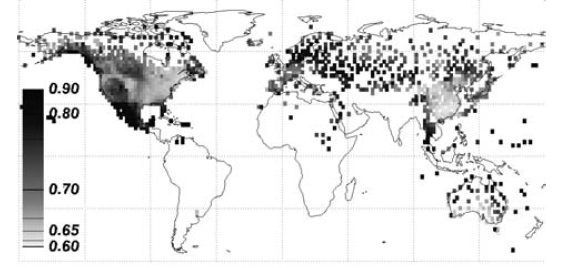
\includegraphics[width=0.8\columnwidth]{../figures/climate.jpg}\\
        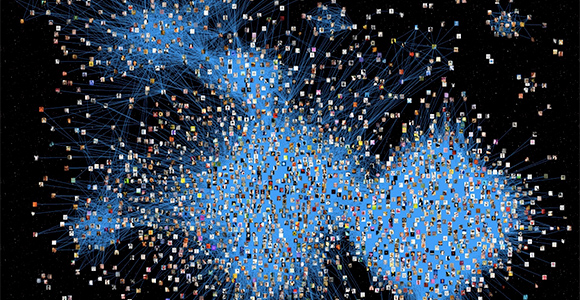
\includegraphics[width=\columnwidth]{../figures/networks-2.jpg}
      \end{column}
      \begin{column}{0.5\textwidth}
        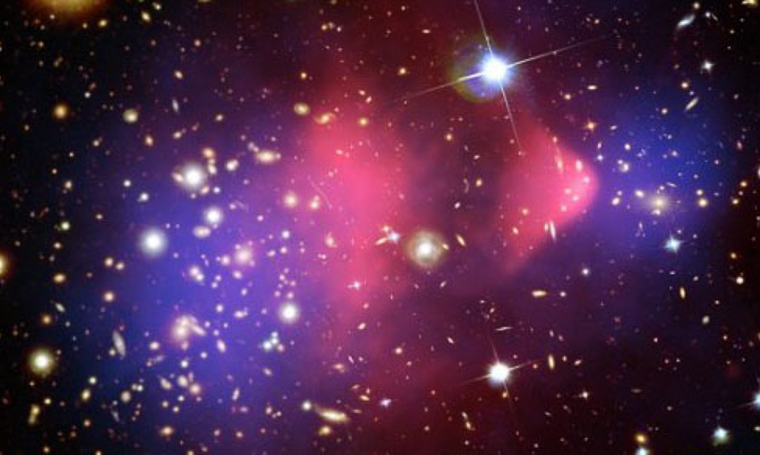
\includegraphics[width=\columnwidth]{../figures/dark_matter.jpg}
        \\
        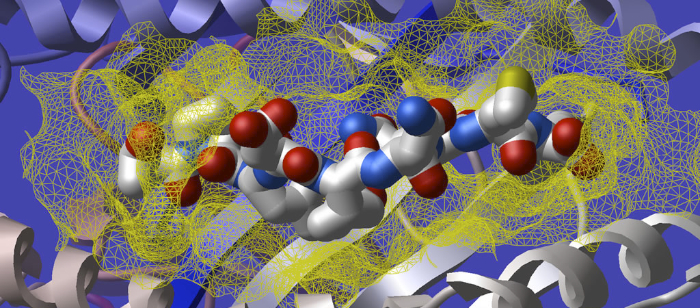
\includegraphics[width=\columnwidth]{../figures/protein.jpg}
      \end{column}
    \end{columns}
    \only<2>{
      \begin{tikzpicture}[remember picture,overlay]
        \draw[fill=black,opacity=0.75] 
        (current page.north east) rectangle (current page.south west);
        \node at (current page.center) {
          {\Huge \alert{Interpretability, Reproducibility}}
        };
      \end{tikzpicture}}
  \end{frame}
}

\only<article>{
  For that reason, science is a very natural application area for
  machine learning.  We can model the effects of climate change and
  how to mitigate it; discover structure in social networks; map
  the existence of dark matter in the universe by intelligently
  shifting through weak gravitational lens data, and not only study
  the mechanisms of protein folding, but discover methods to
  synthesize new drugs.

  We must be careful, however. In many cases we need to be able to
  interpret what our model tells us. We also must make sure that
  the any results we obtain are reproducible. This is something
  that we shall emphasize in this course.
}

\only<presentation>{
  \begin{frame}
    \frametitle{Pervasive ``intelligent'' systems}
    \begin{columns}
      \begin{column}{0.3\textwidth}
        \centering
        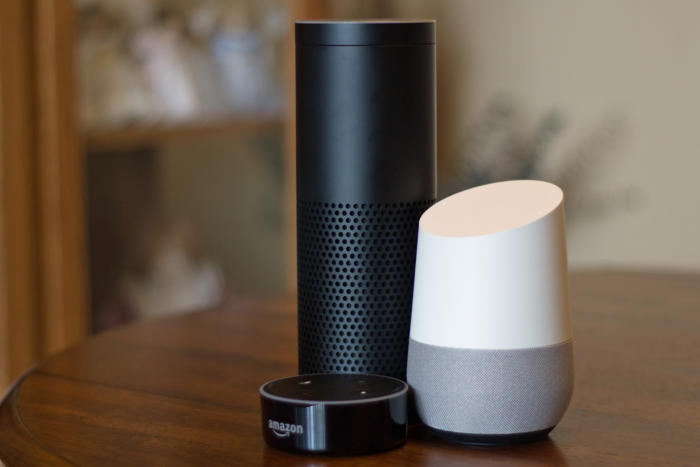
\includegraphics[width=\textwidth]{../figures/echo-home.jpg}
        \\
        Home assistants

        \vspace{\fill}

        \bigskip

        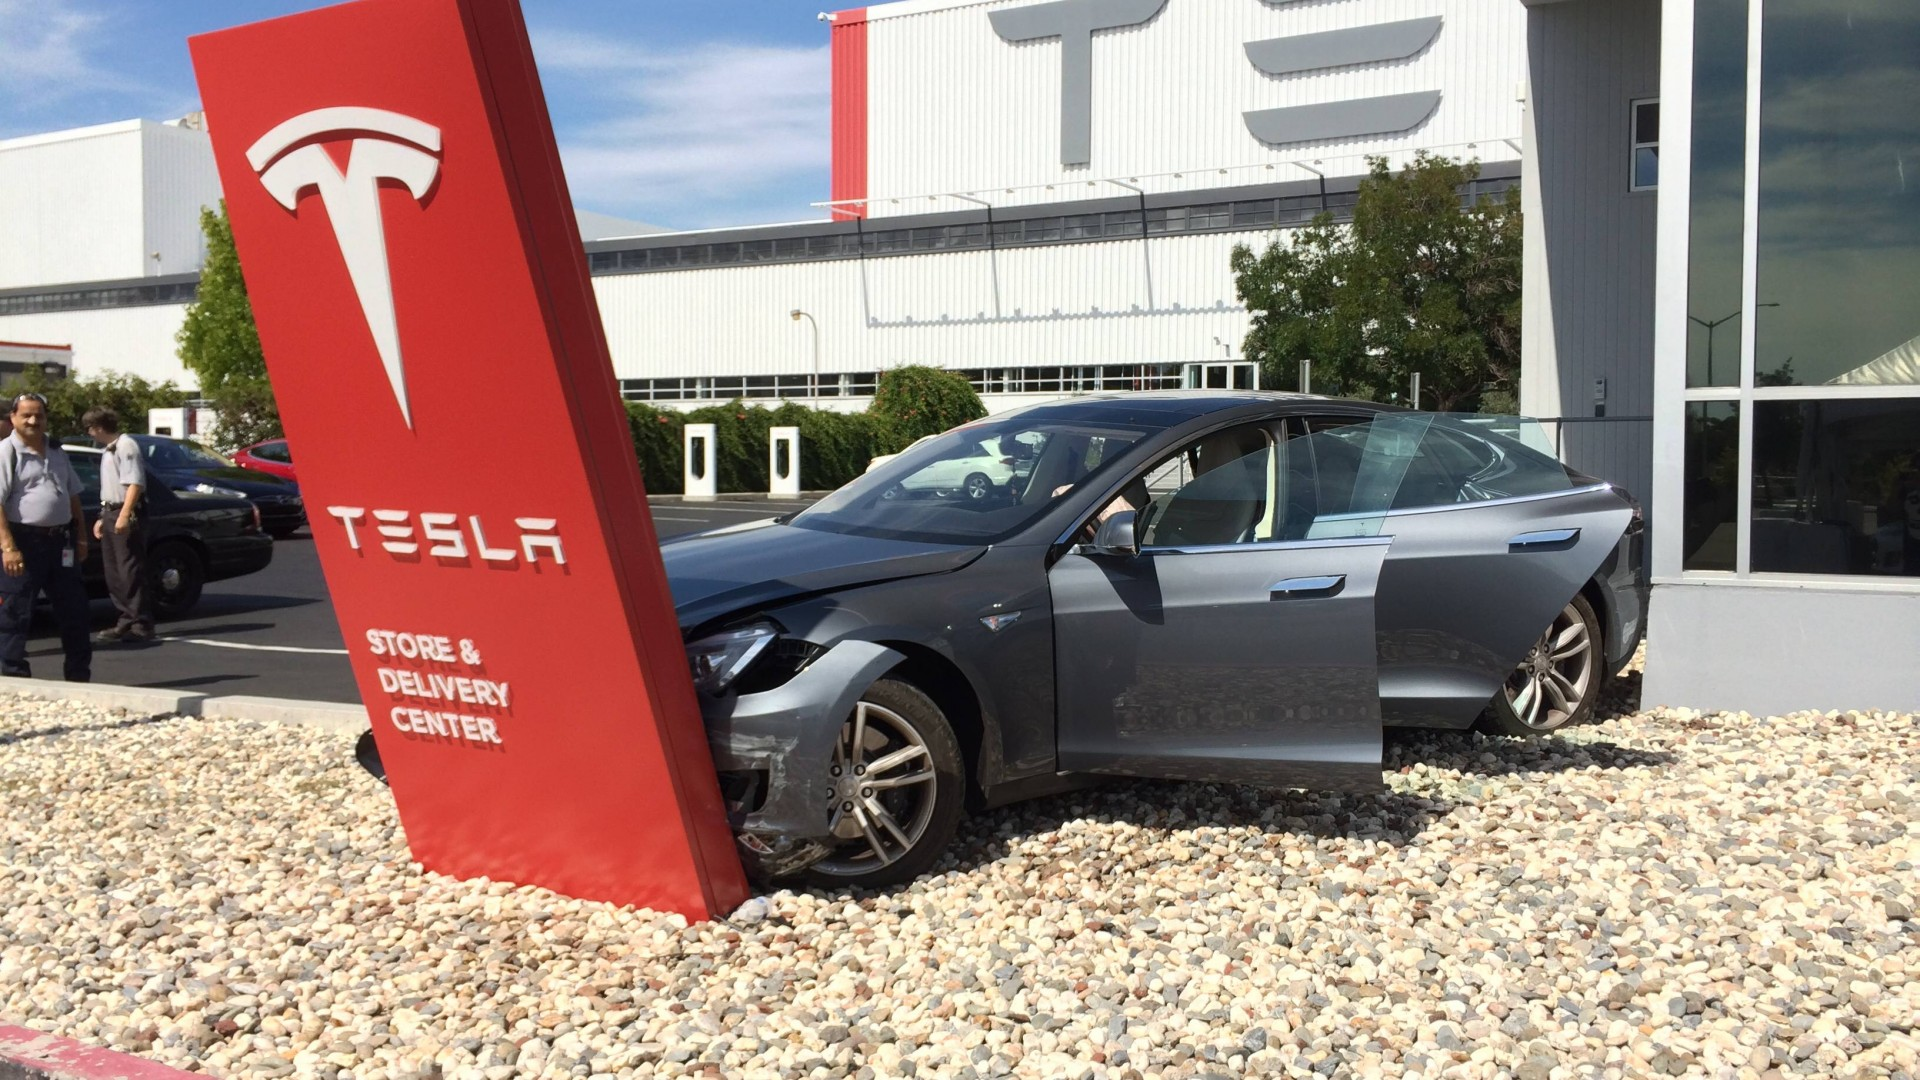
\includegraphics[width=\textwidth]{../figures/tesla.jpg}
        \\
        Autonomous vehicles
      \end{column}
      \begin{column}{0.3\textwidth}
        \centering 
        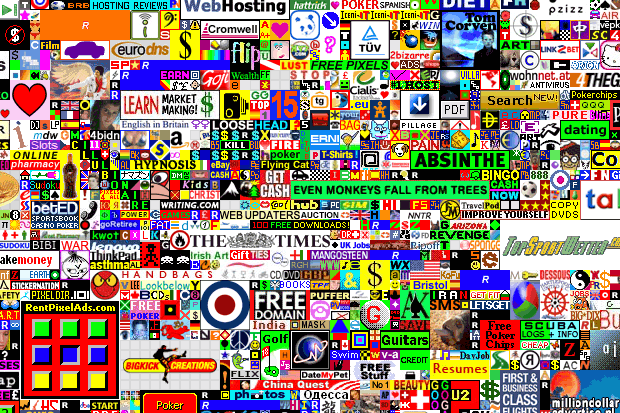
\includegraphics[width=\textwidth]{../figures/web-ads.png}
        \\
        Web advertising

        \vspace{\fill}

        \bigskip

        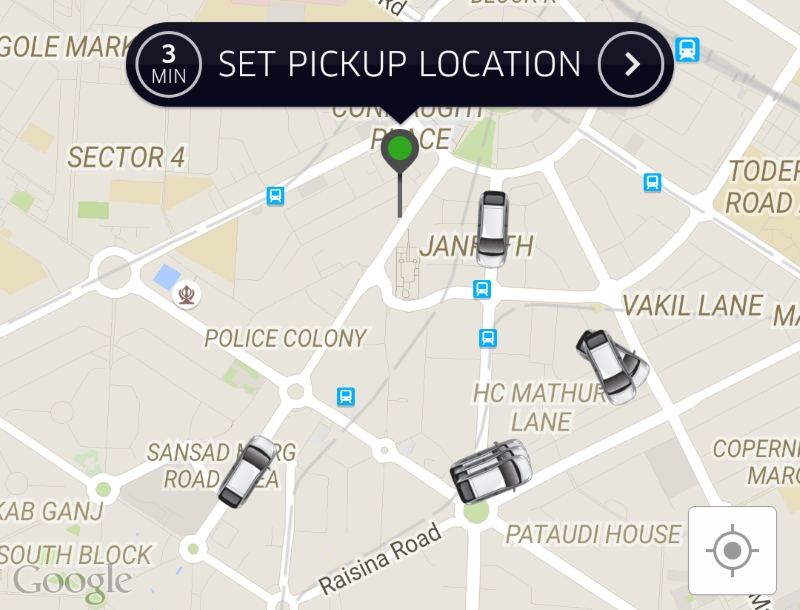
\includegraphics[width=\textwidth]{../figures/uber-here-maps.jpg}
        \\
        Ridesharing
      \end{column}
      \begin{column}{0.3\textwidth}
        \centering 
        \\
        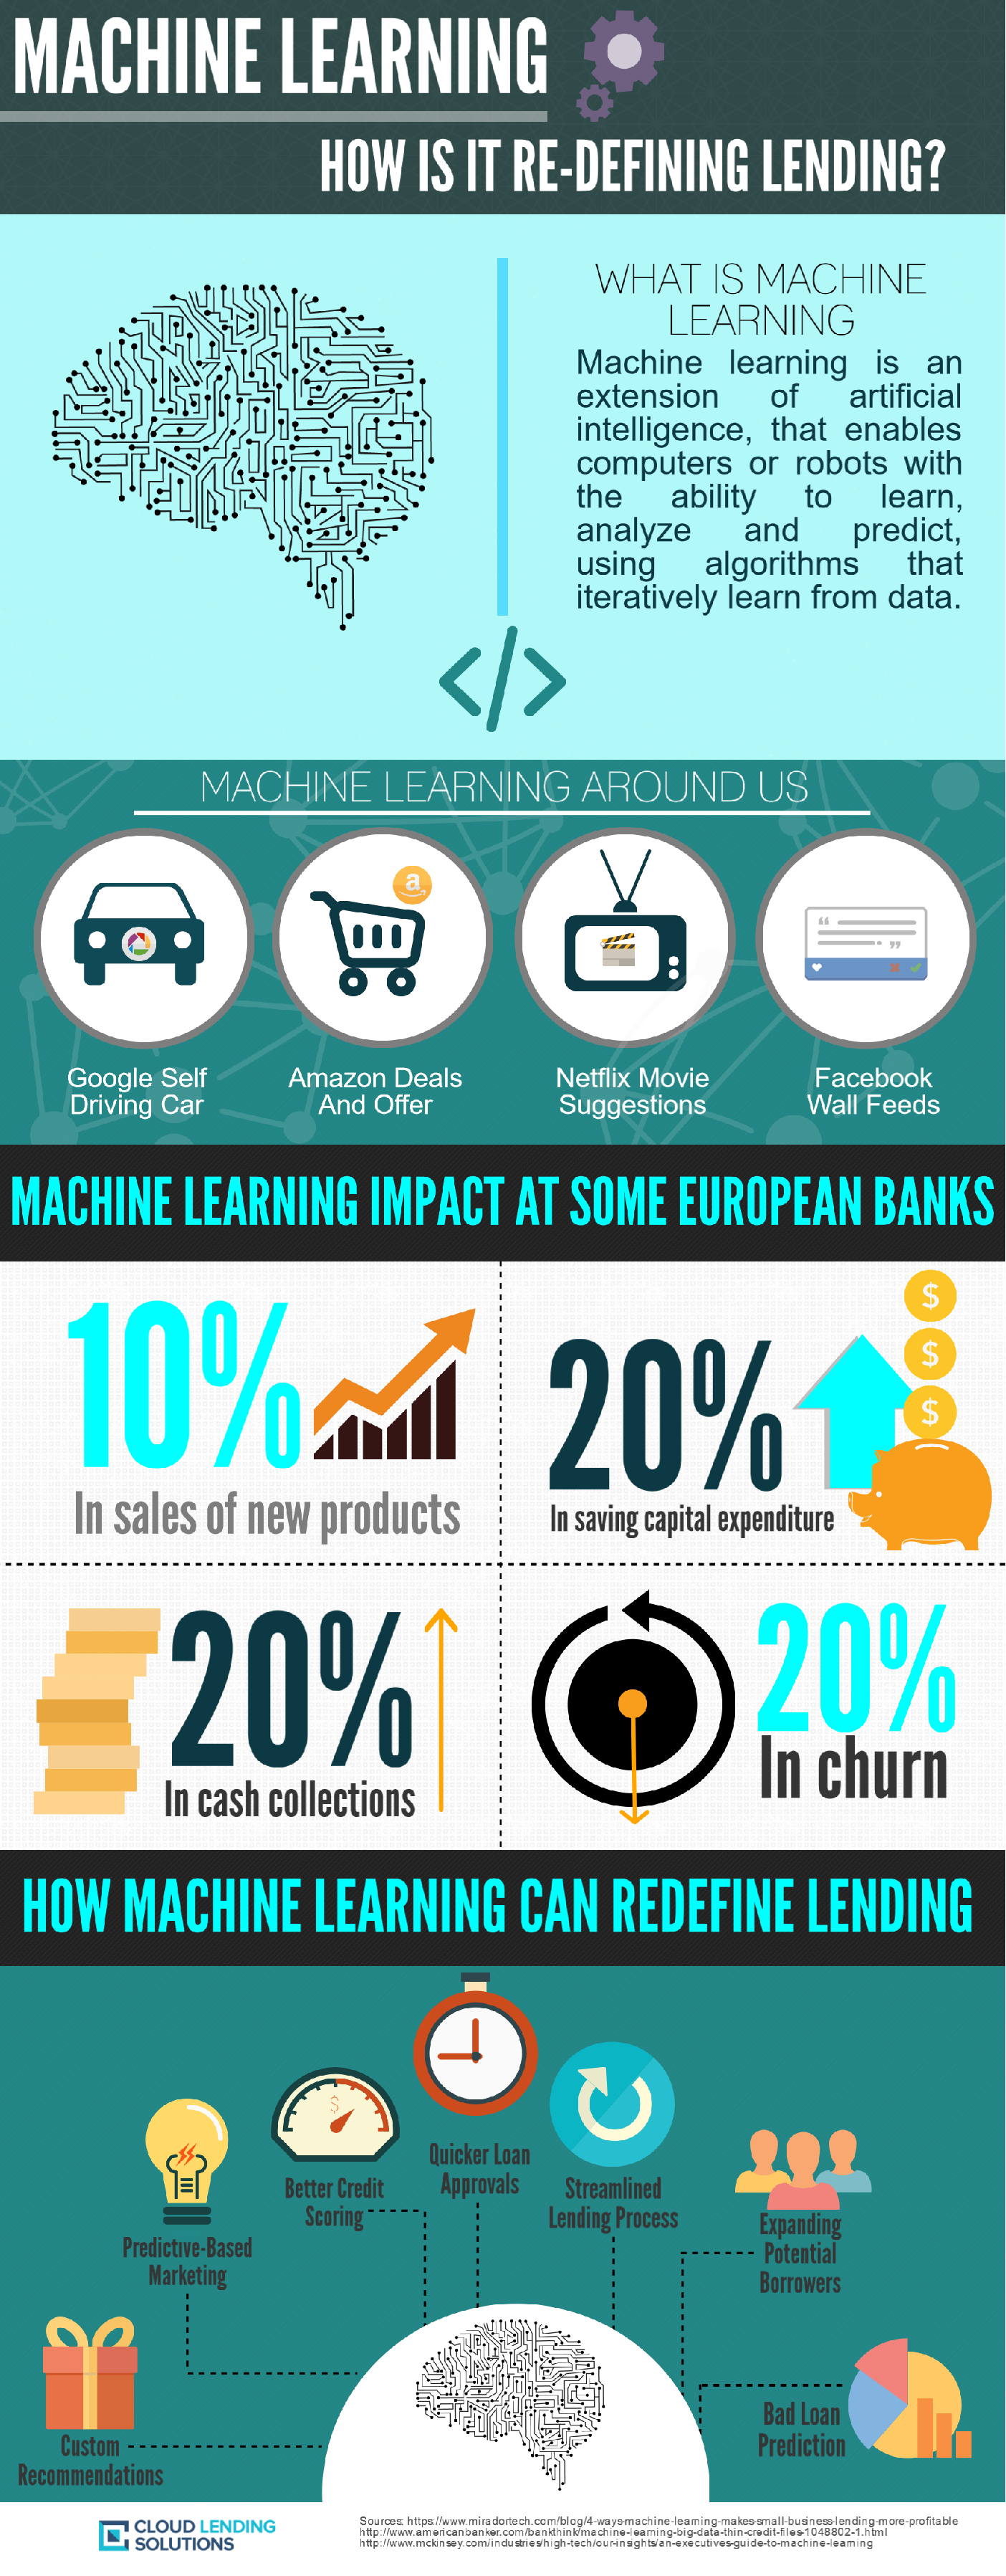
\includegraphics[width=\textwidth,clip = true, trim=0 0 0 42.5cm]{../figures/lending.pdf}
        \\
        Lending

        \vspace{\fill}

        \bigskip

        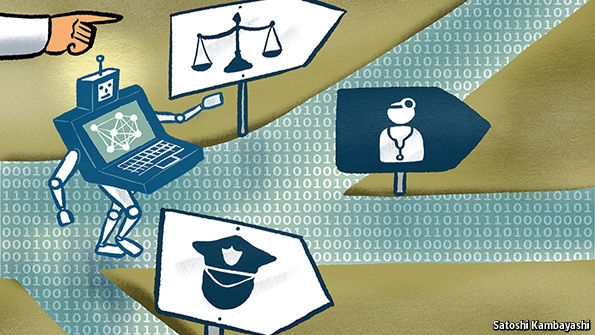
\includegraphics[width=\textwidth]{../figures/algorithms-public.jpg}
        \\
        Public policy
      \end{column}
    \end{columns}
    \only<2>{
      \begin{tikzpicture}[remember picture,overlay]
        \draw[fill=black,opacity=0.75] 
        (current page.north east) rectangle (current page.south west);
        \node at (current page.center) {
          {\Huge \alert{Privacy, Fairness, Safety}}
        };
      \end{tikzpicture}}
  \end{frame}
}

\only<article>{
  While machine learning models in science are typically carefully
  handcrafted by scientists and experts in machine learning and
  statistics, this is not typically the case in everyday
  applications. Nevertheless, well-known or home-grown machine
  learning models are being deployed across the application
  spectrum. This involve home assistants that try and get you want,
  web advertising, which tries to find new things for you to want,
  lending, which tries to optimally lend you money so that you buy
  what you didn't need before. We also have autonomous vehicles,
  which take you were you want to go, and ridesharing services,
  which do the same thing, but use humans instead. Finally, there
  are many applications in public policy, such as crime prevention,
  justice, and disease control which use machine learning.  In all
  those cases, we have to worry about a great many things that are
  outside the scope of the machine learning problems itself. These
  are (a) privacy: you don't want your data used in ways that you have
  not consented to (b) fairness: you don't want minorities to be
  disadvantaged and (c) safety: you don't want your car to crash.
}

\subsection{Data analysis,  learning and planning}

\only<article>{
  To make the above more concrete, let's have a look at a number of problems in machine learning. These involve learning from and analysing data, including inferring decision rules, and constructing complex plans using the evidence gleaned from the data. Machine learning problems are commonly separated in three different types: supervised, unsupervised and reinforcement learning. Typical supervised learning problems include classification and regression, while unsupervised problems include compression, clustering and topic modelling. Reinforcement learning, on the other hand, is concerned with artificially intelligent agents more generally, with examples including game playing and adaptive control. Their main differences are two. Firstly, the \emph{type} of feedback we have about learning performance. Secondly, and perhaps more importantly, whether or not the problem involves \emph{active data collection}. In this course, we will try and take a global view of these problems in the context of decision theory.
}

\only<presentation>{
  \begin{frame}
    \centering
    \Huge{What can machine learning do?}
  \end{frame}
}
\begin{frame}
  \frametitle{Can machines learn from data?}
  \begin{center}
    \only<1>{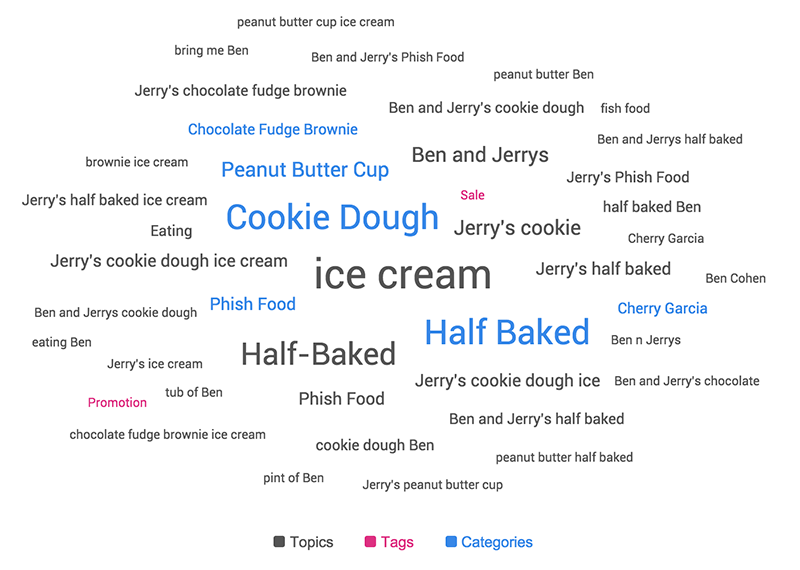
\includegraphics[width=0.8\textwidth]{../figures/text-cloud}
      \\

      {\large An unsupervised learning problem: topic modelling}
    }
    \only<2>{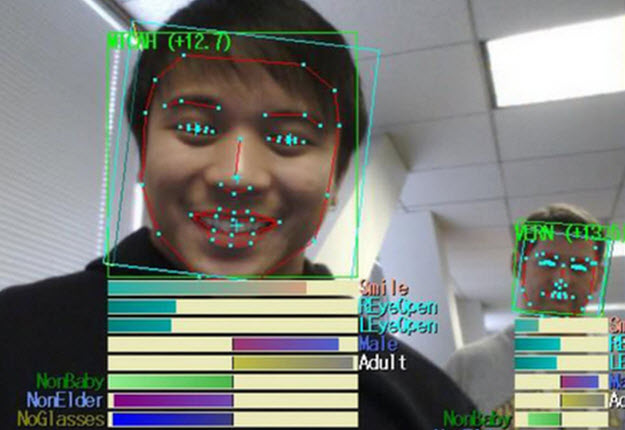
\includegraphics[width=0.8\textwidth]{../figures/Face-Recognition}
      \\

      {\large A supervised learning problem: object recognition}
    }
  \end{center}
\end{frame}


\only<article>{
  You can use machine learning just to analyse, or find structure in
  the data. This is generally called unsupervised learning. One such
  example is topic modelling, where you let the algorithm find topics
  from a corpus of text.  These days machines are used to learn from
  in many applications.  These include speech recognition, facial
  authentication, weather prediction, etc. In general, in these
  problems we are given a \emph{labelled} dataset with, say, example
  images from each class. Unfortunately this does not scale very
  well, because obtaining labels is expensive.

  This is partially how science works, because what we need to do
  is to find a general rule of nature from data. Starting from some
  hypothesis and some data, we reach a conclusion. However, many
  times we may need to actively experiment to obtain more data,
  perhaps because we found that our model is wrong.
}



\begin{frame}
  \frametitle{Can machines learn from their mistakes?}
  \begin{center}
    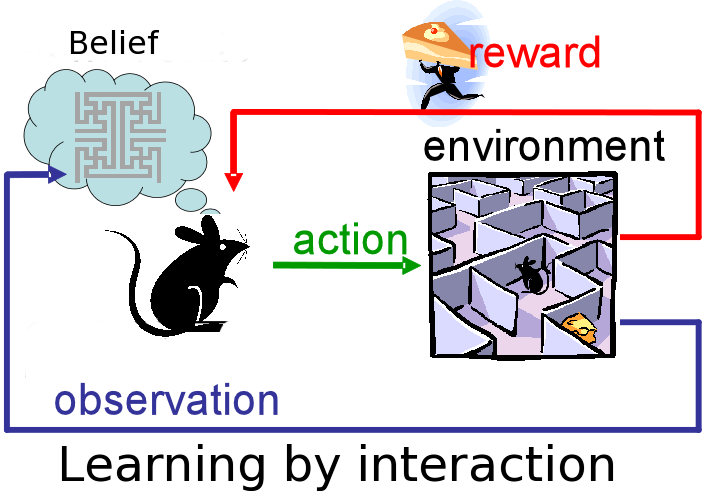
\includegraphics[width=0.7\textwidth]{../figures/rl_interaction}
  \end{center}
  \begin{block}{Reinforcement learning}
    Take actions $a_1, \ldots, a_t$, so as to maximise utility
    $U = \sum_{t=1}^T r_t$
  \end{block}
\end{frame}


\only<article>{
  So, what happens when we make a mistake? Can we somehow recognise
  it? Humans and other animals can actually learn from their
  mistakes. Consider the proverbial rat in the maze. At some
  intervals, the experimenter places some cheese in there, and the
  rat must do a series of actions to obtain it, such as navigating
  the maze and pulling some levers. It doesn't know how to get to
  the cheese easily, but it slowly learns the layout of the maze
  through observation, and in the end, through trial-and-error it
  is able to get to the cheese very efficiently.

  We can formalise this as a reinforcement learning problem, where
  the rat takes a series of actions; at each step it also obtains a
  reward, let's say equal to 0 when it has no cheese, and 1 when it
  eats cheese. Then we can declare that the rat's utility is the sum
  of all rewards over time, i.e. the total amount of cheese it can
  eat before it dies. The rat needs to explore the environment in order to be able to
  get to the cheese. 

  An example in robotics is trying to teach a
  robot to flip pancakes. One easy thing we can try is to show the robot
  how to do it, and then let it just copy the demonstrated
  movement. However, this doesn't work! The robot needs to explore
  variations of the movement, until it manages to successfully flip
  pancakes. Again, we can formulate this as a reinforcement learning
  problem, with a reward that is high whenever the pancake's position is
  flipped, and on the pan; and low everywhere else. Then the robot can
  learn to perform this behaviour through trial and error. It's
  important to note that in this example, merely demonstration is not
  enough. Neither is reinforcement learning enough. The same thing is
  true for the recent success of AlphaGo in beating a master human:
  apart from planning, they used both demonstration data and self-play,
  so that it could learn through trial and error.  }

\begin{frame}
  \frametitle{Can machines make complex plans?}
  \begin{center}
    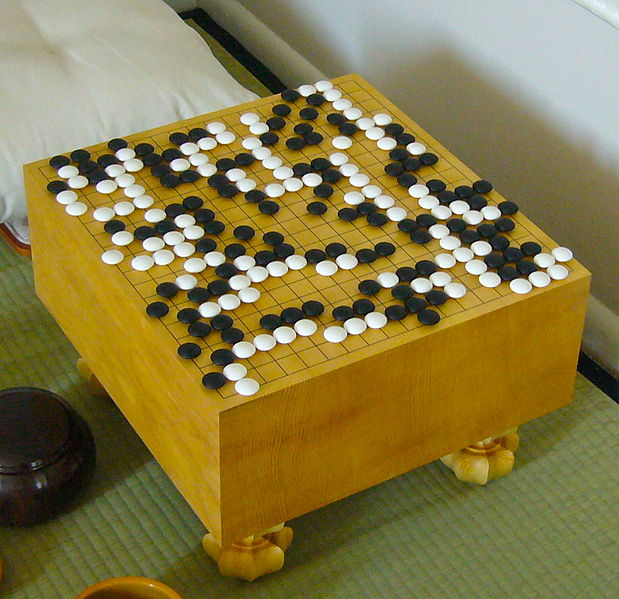
\includegraphics[width=0.8\textwidth]{../figures/619px-FloorGoban}
  \end{center}
\end{frame}


\only<article>{
  I suppose the first question is whether machines can plan
  ahead. Indeed, even for large problems, such as Go, machines can
  now perform at least as well as top-rated humans. How is this
  achieved?
}

\begin{frame}
  \frametitle{Machines can make complex plans!}
  \begin{center}
    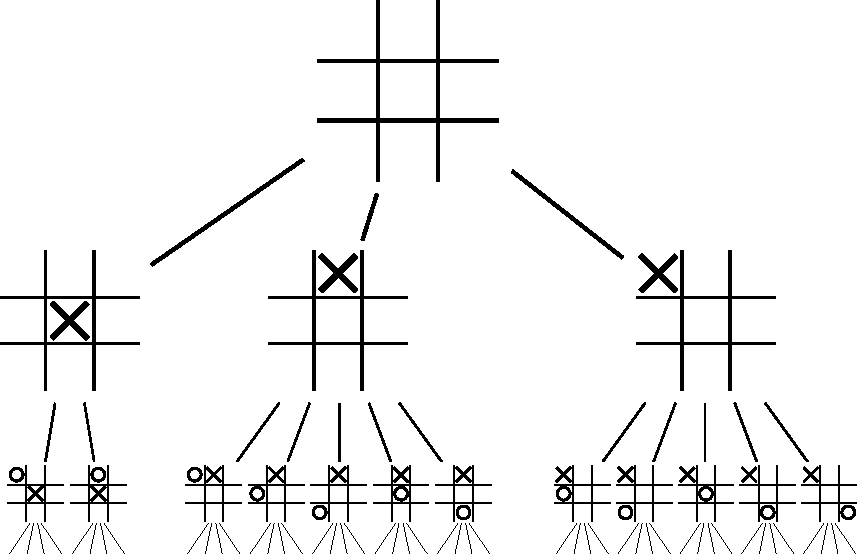
\includegraphics[width=0.8\textwidth]{../figures/Tic-tac-toe-game-tree}
  \end{center}
\end{frame}


\only<article>{
  The basic construction is the planning tree. This is an enumeration
  of all possible future events. If a complete enumeration is
  impossible, a partial tree is constructed. However this requires
  evaluating non-terminal game positions. In the old times, this was
  done with heuristics, but now this is data-driven, both through the
  use of expert databases, and through self-play and reinforcement
  learning.
}


\subsection{Experiment design}

\only<presentation>{
  \begin{frame}
    \centering
    \Huge{The scientific process as machine learning}
  \end{frame}
  \begin{frame}
    \centering
    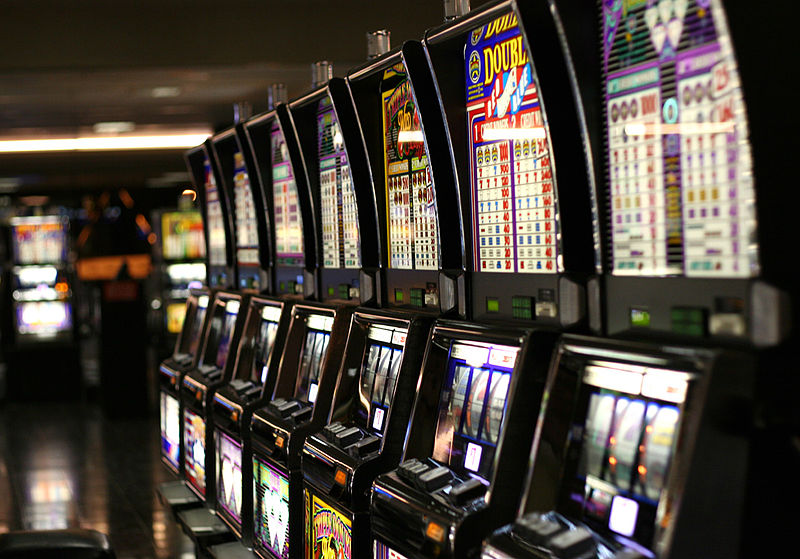
\includegraphics[width=\textwidth]{../figures/Las_Vegas_slot_machines}
  \end{frame}
}


\only<article>{
  An example that typifies trial and error learning are bandit
  problems. Imagine that you are in a Casino and you wish to
  maximise the amount of money you make during the night. There are
  a lot of machines to play. If you knew which one was the best,
  then you'd just play it all night long. However, you must also
  spend time trying out different machines, in order to get an
  estimate of how much money each one gives out. The trade off
  between trying out different machines and playing the one you
  currently think is best is called the exploration-exploitation
  trade-off and it appears in many problems of experiment design for
  science.
}


\begin{frame}
  \frametitle{Adam, the robot scientist}
  \centering
  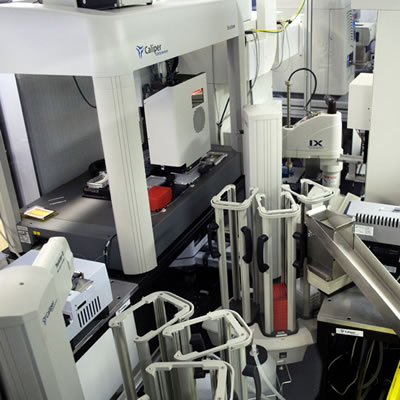
\includegraphics[width=0.8\textwidth]{../figures/robot-scientist}
\end{frame}


\only<article>{
  Let's say we want to build a robot scientist and tell it to
  discover a cure for cancer. What does the scientist do and how can the robot replicate it??
}



\begin{frame}
  \frametitle{Drug discovery}
  \centering
  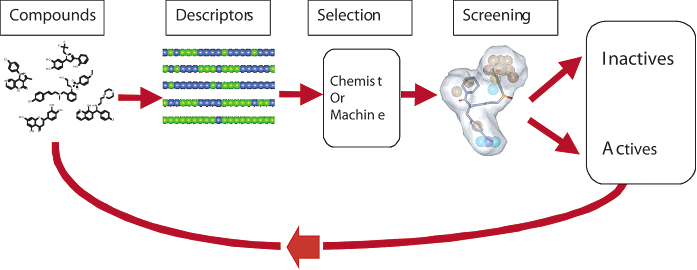
\includegraphics[width=\columnwidth]{../figures/drug-discovery-000}
\end{frame}


\only<article>{
  Simplifying the problem a bit, consider that you have a large
  number of drug candidates for cancer and you wish to discover
  those that are active against it. The ideas is that you select
  some of them, then screen them, to sort them into active and
  inactive. However, there are too many drugs to screen, so the
  process is interactive. At each cycle, we select some drugs to
  screen, classify them, and then use this information to select
  more drugs to screen. This cycle, consequently has two parts:
  1. Selecting some drugs given our current knowledge.
  2. Updating our knowledge given new evidence.
}


\begin{frame}
  \frametitle{Drawing conclusions from results}
  \centering
  \begin{tikzpicture}[line width=2pt]
    \node at (0,0) (bt) {hypothesis};
    \node[select] at (0,2) (at) {experiment};
    \node[utility] at (3,-2) (rt) {result};
    \draw[blue,->] (at) -- (rt);
    \node at (4,0) (bt2) {conclusion};
    \draw[red,->] (at) -- (bt2);
    \draw[red,->] (bt) -- (bt2);
    \draw[red,->] (rt) -- (bt2);
  \end{tikzpicture}
\end{frame}

\only<article>{
  In general, we would like to have some method which can draw
  conclusions from results. This involves starting with a
  hypothesis, performing an experiment to verify or refute it,
  obtain some experimental result; and then concluding for or
  against the hypothesis. Here the arrows show dependencies
  between these variables. So what do we mean by "hypothesis" in this case?
}

\subsection{Bayesian inference.}
\begin{frame}
  \frametitle{Tycho Brahe's minute eye measurements}
  \begin{columns}
    \begin{column}{0.5\textwidth}
      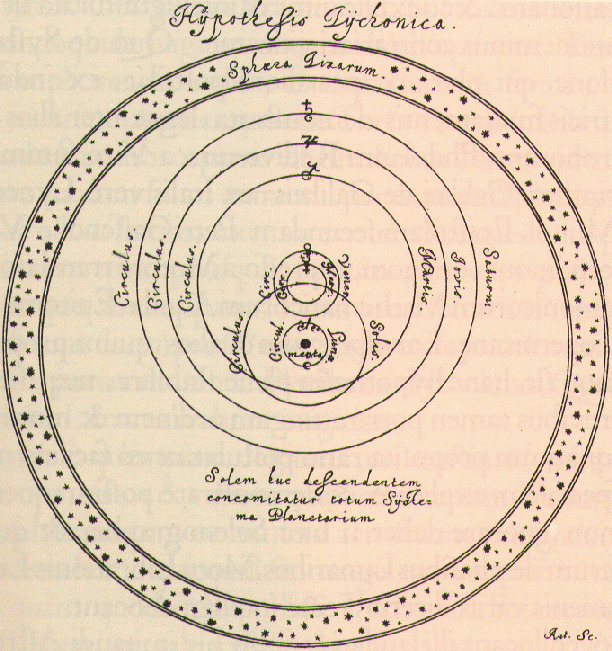
\includegraphics[width=0.5\textwidth]{../figures/circular-orbits}
    \end{column}
    \begin{column}{0.5\textwidth}
      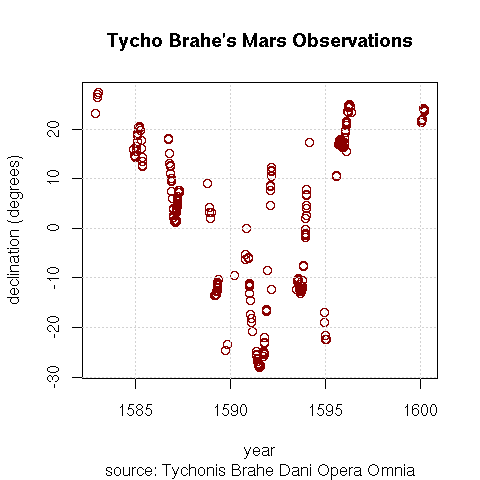
\includegraphics[width=0.5\textwidth]{../figures/tycho-observations}
    \end{column}
  \end{columns}
  \begin{itemize}
  \item Hypothesis: Circular orbits
  \item Conclusion: \alert{Specific} circular orbits
  \end{itemize}
\end{frame}


\only<article>{
  Let's take the example of planetary orbits. Here Tycho famously
  spent 20 years experimentally measuring the location of Mars. He
  had a hypothesis: that planetary orbits were circular, but he
  didn't know which were the right orbits. When he tried to fit his data to this hypothesis, he concluded a specific circular orbit for Mars \ldots around Earth.
}


\begin{frame}
  \frametitle{Johannes Kepler's alternative hypothesis}
  \begin{columns}
    \begin{column}{0.5\textwidth}
      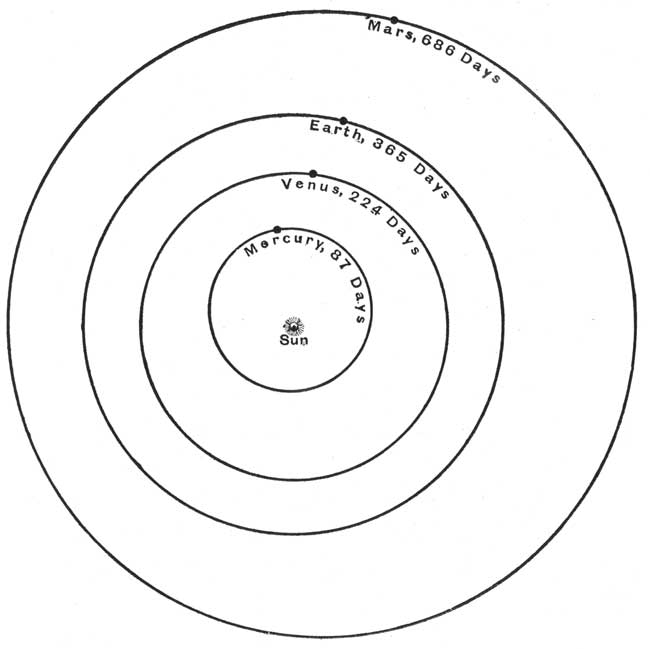
\includegraphics[width=0.5\textwidth]{../figures/orbits}
    \end{column}
    \begin{column}{0.5\textwidth}
      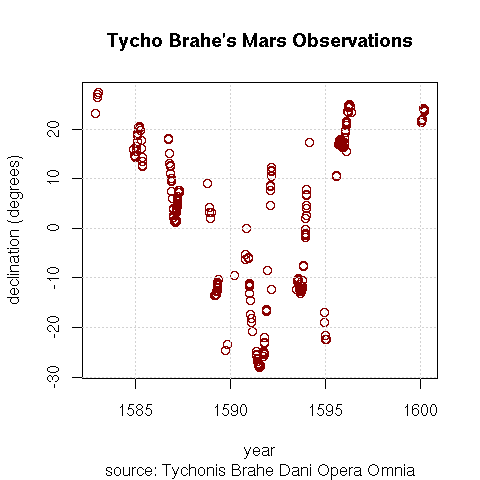
\includegraphics[width=0.5\textwidth]{../figures/tycho-observations}
    \end{column}
  \end{columns}
  \begin{itemize}
  \item Hypothesis: Circular \alert{or} elliptic orbits
  \item Conclusion: Specific \alert{elliptic} orbits
  \end{itemize}
\end{frame}


\only<article>{
  Kepler had a more general hypothesis: that orbits could be
  circular or elliptic, and he actually accepted that the planets
  orbited the sun. This led him to the broadly correct model of all
  planets being in elliptical orbits around the sun. However, the
  actual verification that all things do not revolve around earth,
  requires different experiments.
}


\begin{frame}
  \frametitle{200 years later, Gauss formalised this statistically}
  \begin{columns}
    \begin{column}{0.5\textwidth}
      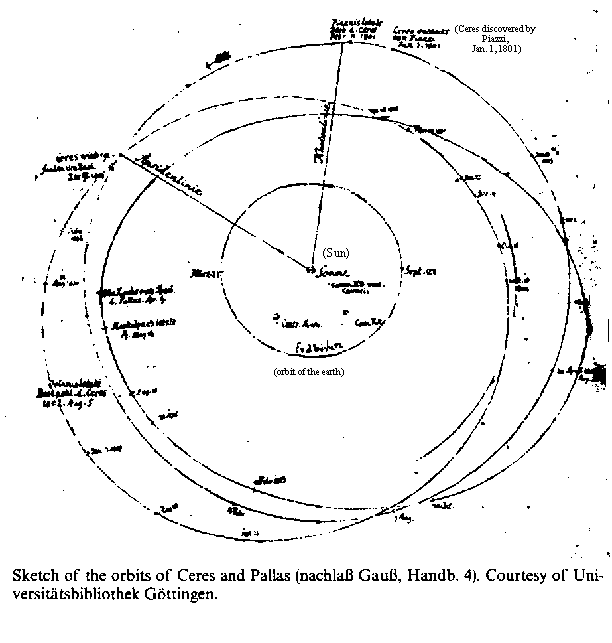
\includegraphics[width=\columnwidth]{../figures/gauss-diagram}
    \end{column}
    \begin{column}{0.5\textwidth}
      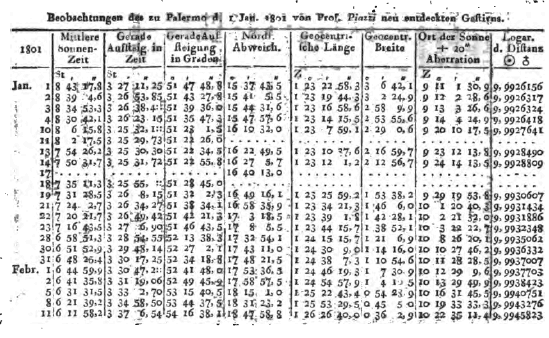
\includegraphics[width=\columnwidth]{../figures/SeptemberTable}
    \end{column}
  \end{columns}
\end{frame}


\only<article>{
  Later on, Gauss collected even more experimental data to calculate the orbit of Ceres. He did this using one of the first formal statistical methods; this allowed him to avoid cheating (like Kepler did, to accentuate his finding that orbits were elliptical).
}


\begin{frame}
  \frametitle{A warning: The dead salmon mirage}
  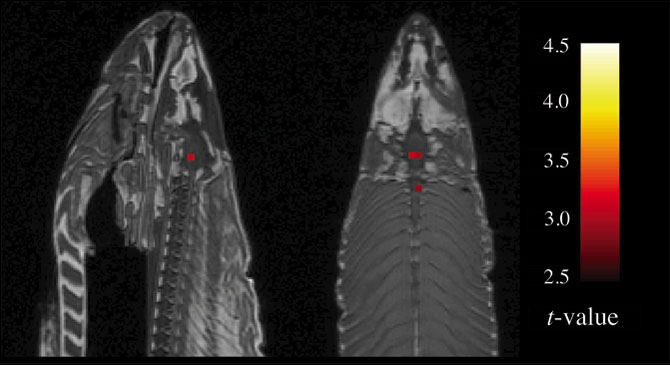
\includegraphics[width=\textwidth]{../figures/fmri-salmon}
\end{frame}


\only<article>{
  It is quite easy to draw the wrong conclusions from applying
  machine learning / statistics to your data. For example, it was
  fashionable to perform fMRI studies in humans to see whether some
  neurons have a particular functional role. There were even
  articles saying that "we found the neurons encoding for Angelina
  Jolie". So some scientists tried to replicate those results. They
  took a dead salmon, and put it an fMRI scanner. They checked its
  brain activity when it was shown images of happy or sad
  people. Perhaps surprisingly, they found an area of the brain that
  was correlated with the pictures - so it seemed, as though the
  dead salmon could distinguish photos of happy people from sad
  ones. However, this was all due to a misapplication of
  statistics. In this course, we will try and teach you to avoid
  such mistakes.
}


\begin{frame}
  \frametitle{Planning future experiments}
  \centering
  \begin{tikzpicture}[line width=2pt]
    \node at (0,0) (bt) {hypothesis};
    \node[select] at (0,2) (at) {experiment};
    \node[utility] at (3,-2) (rt) {result};
    \draw[blue,->] (at) -- (rt);
    \node at (4,0) (bt2) {conclusion};
    \draw[red,->] (at) -- (bt2);
    \draw[red,->] (bt) -- (bt2);
    \draw[red,->] (rt) -- (bt2);
  \end{tikzpicture}
\end{frame}

\only<article>{
  I mentioned before that we must decide what experiment to do. This is indeed difficult, especially in setting such as drug discovery where the number of experiments is huge.  However, conceptually, there is a simple and elegant solution to this problem.
}


\begin{frame}
  \frametitle{Planning experiments is like Tic-Tac-Toe}
  \begin{center}
    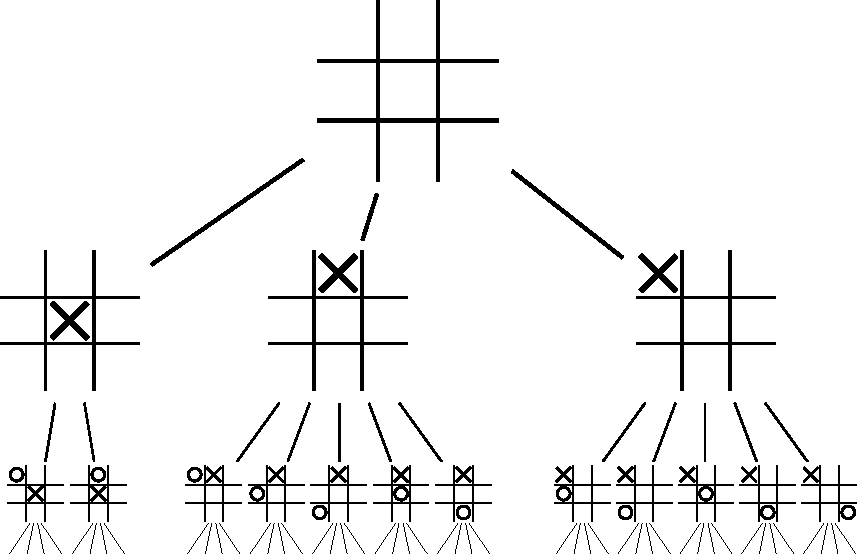
\includegraphics[width=\textwidth]{../figures/Tic-tac-toe-game-tree}
  \end{center}
\end{frame}


\only<article>{
  The basic idea is to think of experiment design as a game between the scientist and Nature. At every step, the scientist plays an X to  denote an experiment. Then Nature responds with an Observation. The main difference from a game is that Nature is (probably) not adversarial. We can also generalise this idea to problems in robotics, etc.
}

\only<presentation>{
  \begin{frame}
    \frametitle{Eve, another robot scientist}
    \centering \movie{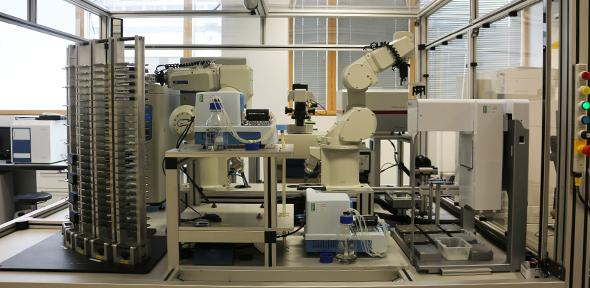
\includegraphics[width=\textwidth]{../figures/eve.jpg}}{Eve-video.mp4}
    Discovered a malaria drug
  \end{frame}
}
\only<article>{
  These kinds of techniques, coming from the reinforcement learning literature have been successfully used at the university of Manchester to create a robot, called Eve, that recently (re)-discovered a malaria drug.
}

\subsection{Course overview}

\begin{frame}
  \frametitle{Machine learning in practice}
  \begin{block}{Avoiding pitfalls}
    \begin{itemize}
    \item Choosing hypotheses.
    \item Correctly interpreting conclusions.
    \item Using a good testing methodology.
    \end{itemize}
  \end{block}
  \begin{block}{Machine learning in society}
    \begin{itemize}
    \item<alert@2> Privacy \uncover<2->{--- Medical data.}
    \item<alert@3> Fairness \uncover<3->{--- Credit risk.}
    \item<alert@4> Safety \uncover<4->{--- Autonomous vehicles.}
    \end{itemize}
  \end{block}
\end{frame}

\only<article>{
  One of the things we want to do in this course is teach you to
  avoid common pitfalls.

  Now I want to get into a different track. So far everything has
  been about pure research, but now machine learning is pervasive:
  Our phones, cars, watches, bathrooms, kettles are connected to the
  internet and send a continuous stream of data to companies. In
  addition, many companies and government actors use machine
  learning algorithms to make or support decisions. This creates a
  number of problems in privacy, fairness and safety.
}


\begin{frame}
  \frametitle{Technical topics}
  
  \begin{block}{Machine learning problems}
    \begin{itemize}
    \item Unsupervised learning.
    \item Supervised learning.
    \item Reinforcement learning.
    \end{itemize}
  \end{block}

  \begin{block}{Machine learning tools}
    \begin{itemize}
    \item Stochastic optimisation and neural networks.
    \item Probabilistic inference and Bayesian networks.
    \item Markov decision processes.
    \end{itemize}
  \end{block}
\end{frame}

\begin{frame}
  \frametitle{Course structure}
  \begin{block}{Module structure}
    \begin{itemize}
    \item \alert{Activity}-based, hands-on.
    \item Background reading \alert{before} class.
    \item Mini-lecture with \alert{Q/A} at each class.
    \item Small \alert{group project} in second half of class.
    \end{itemize}
  \end{block}

  \begin{block}{Modules}
    \begin{itemize}
    \item Medical diagnostics.
    \item Speech recognition.
    \item Recommendation systems.
    \item Helicopter flight.
    \end{itemize}
  \end{block}
\end{frame}


\section{Nearest neighbours}
\begin{frame}
  \frametitle{Discriminating between diseases}
  % Title: glps_renderer figure
% Creator: GL2PS 1.3.8, (C) 1999-2012 C. Geuzaine
% For: Octave
% CreationDate: Fri Jun 16 12:38:10 2017
\begin{pgfpicture}
\pgfsetlinewidth{0.01pt}
\color[rgb]{1.000000,1.000000,1.000000}
\pgfpathmoveto{\pgfpoint{41.600006pt}{205.577454pt}}
\pgflineto{\pgfpoint{289.600037pt}{140.777435pt}}
\pgflineto{\pgfpoint{41.600006pt}{140.777435pt}}
\pgfpathclose
\pgfusepath{fill,stroke}
\pgfpathmoveto{\pgfpoint{41.600006pt}{205.577454pt}}
\pgflineto{\pgfpoint{289.600037pt}{205.577454pt}}
\pgflineto{\pgfpoint{289.600037pt}{140.777435pt}}
\pgfpathclose
\pgfusepath{fill,stroke}
\pgfpathmoveto{\pgfpoint{41.600006pt}{91.199989pt}}
\pgflineto{\pgfpoint{289.600037pt}{26.399979pt}}
\pgflineto{\pgfpoint{41.600006pt}{26.399979pt}}
\pgfpathclose
\pgfusepath{fill,stroke}
\pgfpathmoveto{\pgfpoint{41.600006pt}{91.199989pt}}
\pgflineto{\pgfpoint{289.600037pt}{91.199989pt}}
\pgflineto{\pgfpoint{289.600037pt}{26.399979pt}}
\pgfpathclose
\pgfusepath{fill,stroke}
\color[rgb]{1.000000,0.000000,0.000000}
\pgfpathmoveto{\pgfpoint{287.608032pt}{140.777435pt}}
\pgflineto{\pgfpoint{288.604004pt}{140.777435pt}}
\pgflineto{\pgfpoint{288.604004pt}{142.317886pt}}
\pgfpathclose
\pgfusepath{fill,stroke}
\pgfpathmoveto{\pgfpoint{289.600037pt}{141.234161pt}}
\pgflineto{\pgfpoint{288.604004pt}{142.317886pt}}
\pgflineto{\pgfpoint{288.604004pt}{140.777435pt}}
\pgfpathclose
\pgfusepath{fill,stroke}
\pgfpathmoveto{\pgfpoint{289.600037pt}{140.777435pt}}
\pgflineto{\pgfpoint{289.600037pt}{141.234161pt}}
\pgflineto{\pgfpoint{288.604004pt}{140.777435pt}}
\pgfpathclose
\pgfusepath{fill,stroke}
\pgfpathmoveto{\pgfpoint{283.624115pt}{140.777435pt}}
\pgflineto{\pgfpoint{284.620087pt}{140.777435pt}}
\pgflineto{\pgfpoint{284.620087pt}{140.819778pt}}
\pgfpathclose
\pgfusepath{fill,stroke}
\pgfpathmoveto{\pgfpoint{285.616089pt}{141.090790pt}}
\pgflineto{\pgfpoint{284.620087pt}{140.819778pt}}
\pgflineto{\pgfpoint{284.620087pt}{140.777435pt}}
\pgfpathclose
\pgfusepath{fill,stroke}
\pgfpathmoveto{\pgfpoint{285.616089pt}{140.777435pt}}
\pgflineto{\pgfpoint{285.616089pt}{141.090790pt}}
\pgflineto{\pgfpoint{284.620087pt}{140.777435pt}}
\pgfpathclose
\pgfusepath{fill,stroke}
\pgfpathmoveto{\pgfpoint{286.612061pt}{140.777435pt}}
\pgflineto{\pgfpoint{285.616089pt}{141.090790pt}}
\pgflineto{\pgfpoint{285.616089pt}{140.777435pt}}
\pgfpathclose
\pgfusepath{fill,stroke}
\pgfpathmoveto{\pgfpoint{275.656250pt}{140.777435pt}}
\pgflineto{\pgfpoint{276.652222pt}{140.777435pt}}
\pgflineto{\pgfpoint{276.652222pt}{141.883286pt}}
\pgfpathclose
\pgfusepath{fill,stroke}
\pgfpathmoveto{\pgfpoint{277.648193pt}{145.700470pt}}
\pgflineto{\pgfpoint{276.652222pt}{141.883286pt}}
\pgflineto{\pgfpoint{276.652222pt}{140.777435pt}}
\pgfpathclose
\pgfusepath{fill,stroke}
\pgfpathmoveto{\pgfpoint{277.648193pt}{140.777435pt}}
\pgflineto{\pgfpoint{277.648193pt}{145.700470pt}}
\pgflineto{\pgfpoint{276.652222pt}{140.777435pt}}
\pgfpathclose
\pgfusepath{fill,stroke}
\pgfpathmoveto{\pgfpoint{278.644196pt}{141.350510pt}}
\pgflineto{\pgfpoint{277.648193pt}{145.700470pt}}
\pgflineto{\pgfpoint{277.648193pt}{140.777435pt}}
\pgfpathclose
\pgfusepath{fill,stroke}
\pgfpathmoveto{\pgfpoint{278.644196pt}{140.777435pt}}
\pgflineto{\pgfpoint{278.644196pt}{141.350510pt}}
\pgflineto{\pgfpoint{277.648193pt}{140.777435pt}}
\pgfpathclose
\pgfusepath{fill,stroke}
\pgfpathmoveto{\pgfpoint{279.640167pt}{141.685425pt}}
\pgflineto{\pgfpoint{278.644196pt}{141.350510pt}}
\pgflineto{\pgfpoint{278.644196pt}{140.777435pt}}
\pgfpathclose
\pgfusepath{fill,stroke}
\pgfpathmoveto{\pgfpoint{279.640167pt}{140.777435pt}}
\pgflineto{\pgfpoint{279.640167pt}{141.685425pt}}
\pgflineto{\pgfpoint{278.644196pt}{140.777435pt}}
\pgfpathclose
\pgfusepath{fill,stroke}
\pgfpathmoveto{\pgfpoint{280.636139pt}{140.839111pt}}
\pgflineto{\pgfpoint{279.640167pt}{141.685425pt}}
\pgflineto{\pgfpoint{279.640167pt}{140.777435pt}}
\pgfpathclose
\pgfusepath{fill,stroke}
\pgfpathmoveto{\pgfpoint{280.636139pt}{140.777435pt}}
\pgflineto{\pgfpoint{280.636139pt}{140.839111pt}}
\pgflineto{\pgfpoint{279.640167pt}{140.777435pt}}
\pgfpathclose
\pgfusepath{fill,stroke}
\pgfpathmoveto{\pgfpoint{281.632141pt}{140.783401pt}}
\pgflineto{\pgfpoint{280.636139pt}{140.839111pt}}
\pgflineto{\pgfpoint{280.636139pt}{140.777435pt}}
\pgfpathclose
\pgfusepath{fill,stroke}
\pgfpathmoveto{\pgfpoint{281.632141pt}{140.777435pt}}
\pgflineto{\pgfpoint{281.632141pt}{140.783401pt}}
\pgflineto{\pgfpoint{280.636139pt}{140.777435pt}}
\pgfpathclose
\pgfusepath{fill,stroke}
\pgfpathmoveto{\pgfpoint{282.628113pt}{141.247986pt}}
\pgflineto{\pgfpoint{281.632141pt}{140.783401pt}}
\pgflineto{\pgfpoint{281.632141pt}{140.777435pt}}
\pgfpathclose
\pgfusepath{fill,stroke}
\pgfpathmoveto{\pgfpoint{282.628113pt}{140.777435pt}}
\pgflineto{\pgfpoint{282.628113pt}{141.247986pt}}
\pgflineto{\pgfpoint{281.632141pt}{140.777435pt}}
\pgfpathclose
\pgfusepath{fill,stroke}
\pgfpathmoveto{\pgfpoint{283.624115pt}{140.777435pt}}
\pgflineto{\pgfpoint{282.628113pt}{141.247986pt}}
\pgflineto{\pgfpoint{282.628113pt}{140.777435pt}}
\pgfpathclose
\pgfusepath{fill,stroke}
\pgfpathmoveto{\pgfpoint{262.708435pt}{140.777435pt}}
\pgflineto{\pgfpoint{263.704407pt}{140.777435pt}}
\pgflineto{\pgfpoint{263.704407pt}{149.672318pt}}
\pgfpathclose
\pgfusepath{fill,stroke}
\pgfpathmoveto{\pgfpoint{264.700409pt}{150.470245pt}}
\pgflineto{\pgfpoint{263.704407pt}{149.672318pt}}
\pgflineto{\pgfpoint{263.704407pt}{140.777435pt}}
\pgfpathclose
\pgfusepath{fill,stroke}
\pgfpathmoveto{\pgfpoint{264.700409pt}{140.777435pt}}
\pgflineto{\pgfpoint{264.700409pt}{150.470245pt}}
\pgflineto{\pgfpoint{263.704407pt}{140.777435pt}}
\pgfpathclose
\pgfusepath{fill,stroke}
\pgfpathmoveto{\pgfpoint{265.696411pt}{146.772659pt}}
\pgflineto{\pgfpoint{264.700409pt}{150.470245pt}}
\pgflineto{\pgfpoint{264.700409pt}{140.777435pt}}
\pgfpathclose
\pgfusepath{fill,stroke}
\pgfpathmoveto{\pgfpoint{265.696411pt}{140.777435pt}}
\pgflineto{\pgfpoint{265.696411pt}{146.772659pt}}
\pgflineto{\pgfpoint{264.700409pt}{140.777435pt}}
\pgfpathclose
\pgfusepath{fill,stroke}
\pgfpathmoveto{\pgfpoint{266.692383pt}{141.012543pt}}
\pgflineto{\pgfpoint{265.696411pt}{146.772659pt}}
\pgflineto{\pgfpoint{265.696411pt}{140.777435pt}}
\pgfpathclose
\pgfusepath{fill,stroke}
\pgfpathmoveto{\pgfpoint{266.692383pt}{140.777435pt}}
\pgflineto{\pgfpoint{266.692383pt}{141.012543pt}}
\pgflineto{\pgfpoint{265.696411pt}{140.777435pt}}
\pgfpathclose
\pgfusepath{fill,stroke}
\pgfpathmoveto{\pgfpoint{267.688354pt}{140.947601pt}}
\pgflineto{\pgfpoint{266.692383pt}{141.012543pt}}
\pgflineto{\pgfpoint{266.692383pt}{140.777435pt}}
\pgfpathclose
\pgfusepath{fill,stroke}
\pgfpathmoveto{\pgfpoint{267.688354pt}{140.777435pt}}
\pgflineto{\pgfpoint{267.688354pt}{140.947601pt}}
\pgflineto{\pgfpoint{266.692383pt}{140.777435pt}}
\pgfpathclose
\pgfusepath{fill,stroke}
\pgfpathmoveto{\pgfpoint{268.684326pt}{165.780823pt}}
\pgflineto{\pgfpoint{267.688354pt}{140.947601pt}}
\pgflineto{\pgfpoint{267.688354pt}{140.777435pt}}
\pgfpathclose
\pgfusepath{fill,stroke}
\pgfpathmoveto{\pgfpoint{268.684326pt}{140.777435pt}}
\pgflineto{\pgfpoint{268.684326pt}{165.780823pt}}
\pgflineto{\pgfpoint{267.688354pt}{140.777435pt}}
\pgfpathclose
\pgfusepath{fill,stroke}
\pgfpathmoveto{\pgfpoint{269.680328pt}{142.178589pt}}
\pgflineto{\pgfpoint{268.684326pt}{165.780823pt}}
\pgflineto{\pgfpoint{268.684326pt}{140.777435pt}}
\pgfpathclose
\pgfusepath{fill,stroke}
\pgfpathmoveto{\pgfpoint{269.680328pt}{140.777435pt}}
\pgflineto{\pgfpoint{269.680328pt}{142.178589pt}}
\pgflineto{\pgfpoint{268.684326pt}{140.777435pt}}
\pgfpathclose
\pgfusepath{fill,stroke}
\pgfpathmoveto{\pgfpoint{270.676331pt}{140.852936pt}}
\pgflineto{\pgfpoint{269.680328pt}{142.178589pt}}
\pgflineto{\pgfpoint{269.680328pt}{140.777435pt}}
\pgfpathclose
\pgfusepath{fill,stroke}
\pgfpathmoveto{\pgfpoint{270.676331pt}{140.777435pt}}
\pgflineto{\pgfpoint{270.676331pt}{140.852936pt}}
\pgflineto{\pgfpoint{269.680328pt}{140.777435pt}}
\pgfpathclose
\pgfusepath{fill,stroke}
\pgfpathmoveto{\pgfpoint{271.672302pt}{149.853119pt}}
\pgflineto{\pgfpoint{270.676331pt}{140.852936pt}}
\pgflineto{\pgfpoint{270.676331pt}{140.777435pt}}
\pgfpathclose
\pgfusepath{fill,stroke}
\pgfpathmoveto{\pgfpoint{271.672302pt}{140.777435pt}}
\pgflineto{\pgfpoint{271.672302pt}{149.853119pt}}
\pgflineto{\pgfpoint{270.676331pt}{140.777435pt}}
\pgfpathclose
\pgfusepath{fill,stroke}
\pgfpathmoveto{\pgfpoint{272.668274pt}{167.198486pt}}
\pgflineto{\pgfpoint{271.672302pt}{149.853119pt}}
\pgflineto{\pgfpoint{271.672302pt}{140.777435pt}}
\pgfpathclose
\pgfusepath{fill,stroke}
\pgfpathmoveto{\pgfpoint{272.668274pt}{140.777435pt}}
\pgflineto{\pgfpoint{272.668274pt}{167.198486pt}}
\pgflineto{\pgfpoint{271.672302pt}{140.777435pt}}
\pgfpathclose
\pgfusepath{fill,stroke}
\pgfpathmoveto{\pgfpoint{273.664276pt}{140.777435pt}}
\pgflineto{\pgfpoint{272.668274pt}{167.198486pt}}
\pgflineto{\pgfpoint{272.668274pt}{140.777435pt}}
\pgfpathclose
\pgfusepath{fill,stroke}
\pgfpathmoveto{\pgfpoint{255.736542pt}{140.777435pt}}
\pgflineto{\pgfpoint{256.732544pt}{140.777435pt}}
\pgflineto{\pgfpoint{256.732544pt}{160.055664pt}}
\pgfpathclose
\pgfusepath{fill,stroke}
\pgfpathmoveto{\pgfpoint{257.728516pt}{145.276688pt}}
\pgflineto{\pgfpoint{256.732544pt}{160.055664pt}}
\pgflineto{\pgfpoint{256.732544pt}{140.777435pt}}
\pgfpathclose
\pgfusepath{fill,stroke}
\pgfpathmoveto{\pgfpoint{257.728516pt}{140.777435pt}}
\pgflineto{\pgfpoint{257.728516pt}{145.276688pt}}
\pgflineto{\pgfpoint{256.732544pt}{140.777435pt}}
\pgfpathclose
\pgfusepath{fill,stroke}
\pgfpathmoveto{\pgfpoint{258.724518pt}{145.143265pt}}
\pgflineto{\pgfpoint{257.728516pt}{145.276688pt}}
\pgflineto{\pgfpoint{257.728516pt}{140.777435pt}}
\pgfpathclose
\pgfusepath{fill,stroke}
\pgfpathmoveto{\pgfpoint{258.724518pt}{140.777435pt}}
\pgflineto{\pgfpoint{258.724518pt}{145.143265pt}}
\pgflineto{\pgfpoint{257.728516pt}{140.777435pt}}
\pgfpathclose
\pgfusepath{fill,stroke}
\pgfpathmoveto{\pgfpoint{259.720490pt}{141.107025pt}}
\pgflineto{\pgfpoint{258.724518pt}{145.143265pt}}
\pgflineto{\pgfpoint{258.724518pt}{140.777435pt}}
\pgfpathclose
\pgfusepath{fill,stroke}
\pgfpathmoveto{\pgfpoint{259.720490pt}{140.777435pt}}
\pgflineto{\pgfpoint{259.720490pt}{141.107025pt}}
\pgflineto{\pgfpoint{258.724518pt}{140.777435pt}}
\pgfpathclose
\pgfusepath{fill,stroke}
\pgfpathmoveto{\pgfpoint{260.716492pt}{140.785751pt}}
\pgflineto{\pgfpoint{259.720490pt}{141.107025pt}}
\pgflineto{\pgfpoint{259.720490pt}{140.777435pt}}
\pgfpathclose
\pgfusepath{fill,stroke}
\pgfpathmoveto{\pgfpoint{260.716492pt}{140.777435pt}}
\pgflineto{\pgfpoint{260.716492pt}{140.785751pt}}
\pgflineto{\pgfpoint{259.720490pt}{140.777435pt}}
\pgfpathclose
\pgfusepath{fill,stroke}
\pgfpathmoveto{\pgfpoint{261.712463pt}{140.881470pt}}
\pgflineto{\pgfpoint{260.716492pt}{140.785751pt}}
\pgflineto{\pgfpoint{260.716492pt}{140.777435pt}}
\pgfpathclose
\pgfusepath{fill,stroke}
\pgfpathmoveto{\pgfpoint{261.712463pt}{140.777435pt}}
\pgflineto{\pgfpoint{261.712463pt}{140.881470pt}}
\pgflineto{\pgfpoint{260.716492pt}{140.777435pt}}
\pgfpathclose
\pgfusepath{fill,stroke}
\pgfpathmoveto{\pgfpoint{262.708435pt}{140.777435pt}}
\pgflineto{\pgfpoint{261.712463pt}{140.881470pt}}
\pgflineto{\pgfpoint{261.712463pt}{140.777435pt}}
\pgfpathclose
\pgfusepath{fill,stroke}
\pgfpathmoveto{\pgfpoint{252.748611pt}{140.777435pt}}
\pgflineto{\pgfpoint{253.744598pt}{205.642242pt}}
\pgflineto{\pgfpoint{253.234100pt}{205.642242pt}}
\pgfpathclose
\pgfusepath{fill,stroke}
\pgfpathmoveto{\pgfpoint{252.748611pt}{140.777435pt}}
\pgflineto{\pgfpoint{253.744598pt}{140.777435pt}}
\pgflineto{\pgfpoint{253.744598pt}{205.642242pt}}
\pgfpathclose
\pgfusepath{fill,stroke}
\pgfpathmoveto{\pgfpoint{254.325424pt}{205.642242pt}}
\pgflineto{\pgfpoint{253.744598pt}{205.642242pt}}
\pgflineto{\pgfpoint{253.744598pt}{140.777435pt}}
\pgfpathclose
\pgfusepath{fill,stroke}
\pgfpathmoveto{\pgfpoint{254.740570pt}{140.777435pt}}
\pgflineto{\pgfpoint{254.325424pt}{205.642242pt}}
\pgflineto{\pgfpoint{253.744598pt}{140.777435pt}}
\pgfpathclose
\pgfusepath{fill,stroke}
\pgfpathmoveto{\pgfpoint{254.740570pt}{140.777435pt}}
\pgflineto{\pgfpoint{254.740570pt}{205.642242pt}}
\pgflineto{\pgfpoint{254.325424pt}{205.642242pt}}
\pgfpathclose
\pgfusepath{fill,stroke}
\pgfpathmoveto{\pgfpoint{255.736542pt}{140.777435pt}}
\pgflineto{\pgfpoint{254.740570pt}{205.642242pt}}
\pgflineto{\pgfpoint{254.740570pt}{140.777435pt}}
\pgfpathclose
\pgfusepath{fill,stroke}
\pgfpathmoveto{\pgfpoint{255.736542pt}{140.777435pt}}
\pgflineto{\pgfpoint{255.155716pt}{205.642242pt}}
\pgflineto{\pgfpoint{254.740570pt}{205.642242pt}}
\pgfpathclose
\pgfusepath{fill,stroke}
\pgfpathmoveto{\pgfpoint{244.780731pt}{140.777435pt}}
\pgflineto{\pgfpoint{245.776718pt}{140.777435pt}}
\pgflineto{\pgfpoint{245.776718pt}{140.921082pt}}
\pgfpathclose
\pgfusepath{fill,stroke}
\pgfpathmoveto{\pgfpoint{246.231064pt}{205.642242pt}}
\pgflineto{\pgfpoint{245.776718pt}{140.921082pt}}
\pgflineto{\pgfpoint{245.776718pt}{140.777435pt}}
\pgfpathclose
\pgfusepath{fill,stroke}
\pgfpathmoveto{\pgfpoint{246.231064pt}{205.642242pt}}
\pgflineto{\pgfpoint{246.230515pt}{205.642242pt}}
\pgflineto{\pgfpoint{245.776718pt}{140.921082pt}}
\pgfpathclose
\pgfusepath{fill,stroke}
\pgfpathmoveto{\pgfpoint{246.772705pt}{140.777435pt}}
\pgflineto{\pgfpoint{246.231064pt}{205.642242pt}}
\pgflineto{\pgfpoint{245.776718pt}{140.777435pt}}
\pgfpathclose
\pgfusepath{fill,stroke}
\pgfpathmoveto{\pgfpoint{246.772705pt}{140.777435pt}}
\pgflineto{\pgfpoint{246.772705pt}{205.642242pt}}
\pgflineto{\pgfpoint{246.231064pt}{205.642242pt}}
\pgfpathclose
\pgfusepath{fill,stroke}
\pgfpathmoveto{\pgfpoint{247.768677pt}{144.035980pt}}
\pgflineto{\pgfpoint{246.772705pt}{205.642242pt}}
\pgflineto{\pgfpoint{246.772705pt}{140.777435pt}}
\pgfpathclose
\pgfusepath{fill,stroke}
\pgfpathmoveto{\pgfpoint{247.768677pt}{144.035980pt}}
\pgflineto{\pgfpoint{247.327042pt}{205.642242pt}}
\pgflineto{\pgfpoint{246.772705pt}{205.642242pt}}
\pgfpathclose
\pgfusepath{fill,stroke}
\pgfpathmoveto{\pgfpoint{247.768677pt}{140.777435pt}}
\pgflineto{\pgfpoint{247.768677pt}{144.035980pt}}
\pgflineto{\pgfpoint{246.772705pt}{140.777435pt}}
\pgfpathclose
\pgfusepath{fill,stroke}
\pgfpathmoveto{\pgfpoint{248.764679pt}{140.987183pt}}
\pgflineto{\pgfpoint{247.768677pt}{144.035980pt}}
\pgflineto{\pgfpoint{247.768677pt}{140.777435pt}}
\pgfpathclose
\pgfusepath{fill,stroke}
\pgfpathmoveto{\pgfpoint{248.764679pt}{140.777435pt}}
\pgflineto{\pgfpoint{248.764679pt}{140.987183pt}}
\pgflineto{\pgfpoint{247.768677pt}{140.777435pt}}
\pgfpathclose
\pgfusepath{fill,stroke}
\pgfpathmoveto{\pgfpoint{249.760651pt}{140.861908pt}}
\pgflineto{\pgfpoint{248.764679pt}{140.987183pt}}
\pgflineto{\pgfpoint{248.764679pt}{140.777435pt}}
\pgfpathclose
\pgfusepath{fill,stroke}
\pgfpathmoveto{\pgfpoint{249.760651pt}{140.777435pt}}
\pgflineto{\pgfpoint{249.760651pt}{140.861908pt}}
\pgflineto{\pgfpoint{248.764679pt}{140.777435pt}}
\pgfpathclose
\pgfusepath{fill,stroke}
\pgfpathmoveto{\pgfpoint{250.756638pt}{143.997910pt}}
\pgflineto{\pgfpoint{249.760651pt}{140.861908pt}}
\pgflineto{\pgfpoint{249.760651pt}{140.777435pt}}
\pgfpathclose
\pgfusepath{fill,stroke}
\pgfpathmoveto{\pgfpoint{250.756638pt}{140.777435pt}}
\pgflineto{\pgfpoint{250.756638pt}{143.997910pt}}
\pgflineto{\pgfpoint{249.760651pt}{140.777435pt}}
\pgfpathclose
\pgfusepath{fill,stroke}
\pgfpathmoveto{\pgfpoint{251.752625pt}{140.777435pt}}
\pgflineto{\pgfpoint{250.756638pt}{143.997910pt}}
\pgflineto{\pgfpoint{250.756638pt}{140.777435pt}}
\pgfpathclose
\pgfusepath{fill,stroke}
\pgfpathmoveto{\pgfpoint{241.792786pt}{140.777435pt}}
\pgflineto{\pgfpoint{242.788757pt}{140.777435pt}}
\pgflineto{\pgfpoint{242.788757pt}{141.050537pt}}
\pgfpathclose
\pgfusepath{fill,stroke}
\pgfpathmoveto{\pgfpoint{243.784744pt}{140.826157pt}}
\pgflineto{\pgfpoint{242.788757pt}{141.050537pt}}
\pgflineto{\pgfpoint{242.788757pt}{140.777435pt}}
\pgfpathclose
\pgfusepath{fill,stroke}
\pgfpathmoveto{\pgfpoint{243.784744pt}{140.777435pt}}
\pgflineto{\pgfpoint{243.784744pt}{140.826157pt}}
\pgflineto{\pgfpoint{242.788757pt}{140.777435pt}}
\pgfpathclose
\pgfusepath{fill,stroke}
\pgfpathmoveto{\pgfpoint{244.780731pt}{140.777435pt}}
\pgflineto{\pgfpoint{243.784744pt}{140.826157pt}}
\pgflineto{\pgfpoint{243.784744pt}{140.777435pt}}
\pgfpathclose
\pgfusepath{fill,stroke}
\pgfpathmoveto{\pgfpoint{239.800812pt}{140.777435pt}}
\pgflineto{\pgfpoint{240.796814pt}{140.777435pt}}
\pgflineto{\pgfpoint{240.796814pt}{141.635849pt}}
\pgfpathclose
\pgfusepath{fill,stroke}
\pgfpathmoveto{\pgfpoint{241.792786pt}{140.777435pt}}
\pgflineto{\pgfpoint{240.796814pt}{141.635849pt}}
\pgflineto{\pgfpoint{240.796814pt}{140.777435pt}}
\pgfpathclose
\pgfusepath{fill,stroke}
\pgfpathmoveto{\pgfpoint{232.828934pt}{140.777435pt}}
\pgflineto{\pgfpoint{233.824921pt}{140.777435pt}}
\pgflineto{\pgfpoint{233.824921pt}{143.663483pt}}
\pgfpathclose
\pgfusepath{fill,stroke}
\pgfpathmoveto{\pgfpoint{234.820892pt}{144.424850pt}}
\pgflineto{\pgfpoint{233.824921pt}{143.663483pt}}
\pgflineto{\pgfpoint{233.824921pt}{140.777435pt}}
\pgfpathclose
\pgfusepath{fill,stroke}
\pgfpathmoveto{\pgfpoint{234.820892pt}{140.777435pt}}
\pgflineto{\pgfpoint{234.820892pt}{144.424850pt}}
\pgflineto{\pgfpoint{233.824921pt}{140.777435pt}}
\pgfpathclose
\pgfusepath{fill,stroke}
\pgfpathmoveto{\pgfpoint{235.816864pt}{141.070068pt}}
\pgflineto{\pgfpoint{234.820892pt}{144.424850pt}}
\pgflineto{\pgfpoint{234.820892pt}{140.777435pt}}
\pgfpathclose
\pgfusepath{fill,stroke}
\pgfpathmoveto{\pgfpoint{235.816864pt}{140.777435pt}}
\pgflineto{\pgfpoint{235.816864pt}{141.070068pt}}
\pgflineto{\pgfpoint{234.820892pt}{140.777435pt}}
\pgfpathclose
\pgfusepath{fill,stroke}
\pgfpathmoveto{\pgfpoint{236.812866pt}{141.387177pt}}
\pgflineto{\pgfpoint{235.816864pt}{141.070068pt}}
\pgflineto{\pgfpoint{235.816864pt}{140.777435pt}}
\pgfpathclose
\pgfusepath{fill,stroke}
\pgfpathmoveto{\pgfpoint{236.812866pt}{140.777435pt}}
\pgflineto{\pgfpoint{236.812866pt}{141.387177pt}}
\pgflineto{\pgfpoint{235.816864pt}{140.777435pt}}
\pgfpathclose
\pgfusepath{fill,stroke}
\pgfpathmoveto{\pgfpoint{237.808838pt}{141.605896pt}}
\pgflineto{\pgfpoint{236.812866pt}{141.387177pt}}
\pgflineto{\pgfpoint{236.812866pt}{140.777435pt}}
\pgfpathclose
\pgfusepath{fill,stroke}
\pgfpathmoveto{\pgfpoint{237.808838pt}{140.777435pt}}
\pgflineto{\pgfpoint{237.808838pt}{141.605896pt}}
\pgflineto{\pgfpoint{236.812866pt}{140.777435pt}}
\pgfpathclose
\pgfusepath{fill,stroke}
\pgfpathmoveto{\pgfpoint{238.804825pt}{141.892487pt}}
\pgflineto{\pgfpoint{237.808838pt}{141.605896pt}}
\pgflineto{\pgfpoint{237.808838pt}{140.777435pt}}
\pgfpathclose
\pgfusepath{fill,stroke}
\pgfpathmoveto{\pgfpoint{238.804825pt}{140.777435pt}}
\pgflineto{\pgfpoint{238.804825pt}{141.892487pt}}
\pgflineto{\pgfpoint{237.808838pt}{140.777435pt}}
\pgfpathclose
\pgfusepath{fill,stroke}
\pgfpathmoveto{\pgfpoint{239.800812pt}{140.777435pt}}
\pgflineto{\pgfpoint{238.804825pt}{141.892487pt}}
\pgflineto{\pgfpoint{238.804825pt}{140.777435pt}}
\pgfpathclose
\pgfusepath{fill,stroke}
\pgfpathmoveto{\pgfpoint{226.853027pt}{140.777435pt}}
\pgflineto{\pgfpoint{227.849014pt}{140.777435pt}}
\pgflineto{\pgfpoint{227.849014pt}{141.269379pt}}
\pgfpathclose
\pgfusepath{fill,stroke}
\pgfpathmoveto{\pgfpoint{228.845001pt}{143.487183pt}}
\pgflineto{\pgfpoint{227.849014pt}{141.269379pt}}
\pgflineto{\pgfpoint{227.849014pt}{140.777435pt}}
\pgfpathclose
\pgfusepath{fill,stroke}
\pgfpathmoveto{\pgfpoint{228.845001pt}{140.777435pt}}
\pgflineto{\pgfpoint{228.845001pt}{143.487183pt}}
\pgflineto{\pgfpoint{227.849014pt}{140.777435pt}}
\pgfpathclose
\pgfusepath{fill,stroke}
\pgfpathmoveto{\pgfpoint{229.840973pt}{143.864670pt}}
\pgflineto{\pgfpoint{228.845001pt}{143.487183pt}}
\pgflineto{\pgfpoint{228.845001pt}{140.777435pt}}
\pgfpathclose
\pgfusepath{fill,stroke}
\pgfpathmoveto{\pgfpoint{229.840973pt}{140.777435pt}}
\pgflineto{\pgfpoint{229.840973pt}{143.864670pt}}
\pgflineto{\pgfpoint{228.845001pt}{140.777435pt}}
\pgfpathclose
\pgfusepath{fill,stroke}
\pgfpathmoveto{\pgfpoint{230.836945pt}{141.428329pt}}
\pgflineto{\pgfpoint{229.840973pt}{143.864670pt}}
\pgflineto{\pgfpoint{229.840973pt}{140.777435pt}}
\pgfpathclose
\pgfusepath{fill,stroke}
\pgfpathmoveto{\pgfpoint{230.836945pt}{140.777435pt}}
\pgflineto{\pgfpoint{230.836945pt}{141.428329pt}}
\pgflineto{\pgfpoint{229.840973pt}{140.777435pt}}
\pgfpathclose
\pgfusepath{fill,stroke}
\pgfpathmoveto{\pgfpoint{231.832932pt}{162.511902pt}}
\pgflineto{\pgfpoint{230.836945pt}{141.428329pt}}
\pgflineto{\pgfpoint{230.836945pt}{140.777435pt}}
\pgfpathclose
\pgfusepath{fill,stroke}
\pgfpathmoveto{\pgfpoint{231.832932pt}{140.777435pt}}
\pgflineto{\pgfpoint{231.832932pt}{162.511902pt}}
\pgflineto{\pgfpoint{230.836945pt}{140.777435pt}}
\pgfpathclose
\pgfusepath{fill,stroke}
\pgfpathmoveto{\pgfpoint{232.828934pt}{140.777435pt}}
\pgflineto{\pgfpoint{231.832932pt}{162.511902pt}}
\pgflineto{\pgfpoint{231.832932pt}{140.777435pt}}
\pgfpathclose
\pgfusepath{fill,stroke}
\pgfpathmoveto{\pgfpoint{222.869080pt}{140.777435pt}}
\pgflineto{\pgfpoint{223.865082pt}{140.777435pt}}
\pgflineto{\pgfpoint{223.865082pt}{142.648438pt}}
\pgfpathclose
\pgfusepath{fill,stroke}
\pgfpathmoveto{\pgfpoint{224.861053pt}{140.814316pt}}
\pgflineto{\pgfpoint{223.865082pt}{142.648438pt}}
\pgflineto{\pgfpoint{223.865082pt}{140.777435pt}}
\pgfpathclose
\pgfusepath{fill,stroke}
\pgfpathmoveto{\pgfpoint{224.861053pt}{140.777435pt}}
\pgflineto{\pgfpoint{224.861053pt}{140.814316pt}}
\pgflineto{\pgfpoint{223.865082pt}{140.777435pt}}
\pgfpathclose
\pgfusepath{fill,stroke}
\pgfpathmoveto{\pgfpoint{225.857040pt}{142.893295pt}}
\pgflineto{\pgfpoint{224.861053pt}{140.814316pt}}
\pgflineto{\pgfpoint{224.861053pt}{140.777435pt}}
\pgfpathclose
\pgfusepath{fill,stroke}
\pgfpathmoveto{\pgfpoint{225.857040pt}{140.777435pt}}
\pgflineto{\pgfpoint{225.857040pt}{142.893295pt}}
\pgflineto{\pgfpoint{224.861053pt}{140.777435pt}}
\pgfpathclose
\pgfusepath{fill,stroke}
\pgfpathmoveto{\pgfpoint{226.853027pt}{140.777435pt}}
\pgflineto{\pgfpoint{225.857040pt}{142.893295pt}}
\pgflineto{\pgfpoint{225.857040pt}{140.777435pt}}
\pgfpathclose
\pgfusepath{fill,stroke}
\pgfpathmoveto{\pgfpoint{218.885147pt}{140.777435pt}}
\pgflineto{\pgfpoint{219.881134pt}{140.777435pt}}
\pgflineto{\pgfpoint{219.881134pt}{141.240646pt}}
\pgfpathclose
\pgfusepath{fill,stroke}
\pgfpathmoveto{\pgfpoint{220.877121pt}{140.777435pt}}
\pgflineto{\pgfpoint{219.881134pt}{141.240646pt}}
\pgflineto{\pgfpoint{219.881134pt}{140.777435pt}}
\pgfpathclose
\pgfusepath{fill,stroke}
\pgfpathmoveto{\pgfpoint{216.893188pt}{140.777435pt}}
\pgflineto{\pgfpoint{217.889160pt}{140.777435pt}}
\pgflineto{\pgfpoint{217.889160pt}{144.868698pt}}
\pgfpathclose
\pgfusepath{fill,stroke}
\pgfpathmoveto{\pgfpoint{218.885147pt}{140.777435pt}}
\pgflineto{\pgfpoint{217.889160pt}{144.868698pt}}
\pgflineto{\pgfpoint{217.889160pt}{140.777435pt}}
\pgfpathclose
\pgfusepath{fill,stroke}
\pgfpathmoveto{\pgfpoint{207.929337pt}{140.777435pt}}
\pgflineto{\pgfpoint{208.925323pt}{140.777435pt}}
\pgflineto{\pgfpoint{208.925323pt}{168.977936pt}}
\pgfpathclose
\pgfusepath{fill,stroke}
\pgfpathmoveto{\pgfpoint{209.716339pt}{205.642242pt}}
\pgflineto{\pgfpoint{208.925323pt}{168.977936pt}}
\pgflineto{\pgfpoint{208.925323pt}{140.777435pt}}
\pgfpathclose
\pgfusepath{fill,stroke}
\pgfpathmoveto{\pgfpoint{209.716339pt}{205.642242pt}}
\pgflineto{\pgfpoint{209.608246pt}{205.642242pt}}
\pgflineto{\pgfpoint{208.925323pt}{168.977936pt}}
\pgfpathclose
\pgfusepath{fill,stroke}
\pgfpathmoveto{\pgfpoint{209.921295pt}{140.777435pt}}
\pgflineto{\pgfpoint{209.716339pt}{205.642242pt}}
\pgflineto{\pgfpoint{208.925323pt}{140.777435pt}}
\pgfpathclose
\pgfusepath{fill,stroke}
\pgfpathmoveto{\pgfpoint{209.921295pt}{140.777435pt}}
\pgflineto{\pgfpoint{209.921295pt}{205.642242pt}}
\pgflineto{\pgfpoint{209.716339pt}{205.642242pt}}
\pgfpathclose
\pgfusepath{fill,stroke}
\pgfpathmoveto{\pgfpoint{210.917267pt}{156.156219pt}}
\pgflineto{\pgfpoint{209.921295pt}{205.642242pt}}
\pgflineto{\pgfpoint{209.921295pt}{140.777435pt}}
\pgfpathclose
\pgfusepath{fill,stroke}
\pgfpathmoveto{\pgfpoint{210.917267pt}{156.156219pt}}
\pgflineto{\pgfpoint{210.173798pt}{205.642242pt}}
\pgflineto{\pgfpoint{209.921295pt}{205.642242pt}}
\pgfpathclose
\pgfusepath{fill,stroke}
\pgfpathmoveto{\pgfpoint{210.917267pt}{140.777435pt}}
\pgflineto{\pgfpoint{210.917267pt}{156.156219pt}}
\pgflineto{\pgfpoint{209.921295pt}{140.777435pt}}
\pgfpathclose
\pgfusepath{fill,stroke}
\pgfpathmoveto{\pgfpoint{211.913269pt}{142.768951pt}}
\pgflineto{\pgfpoint{210.917267pt}{156.156219pt}}
\pgflineto{\pgfpoint{210.917267pt}{140.777435pt}}
\pgfpathclose
\pgfusepath{fill,stroke}
\pgfpathmoveto{\pgfpoint{211.913269pt}{140.777435pt}}
\pgflineto{\pgfpoint{211.913269pt}{142.768951pt}}
\pgflineto{\pgfpoint{210.917267pt}{140.777435pt}}
\pgfpathclose
\pgfusepath{fill,stroke}
\pgfpathmoveto{\pgfpoint{212.909241pt}{140.796997pt}}
\pgflineto{\pgfpoint{211.913269pt}{142.768951pt}}
\pgflineto{\pgfpoint{211.913269pt}{140.777435pt}}
\pgfpathclose
\pgfusepath{fill,stroke}
\pgfpathmoveto{\pgfpoint{212.909241pt}{140.777435pt}}
\pgflineto{\pgfpoint{212.909241pt}{140.796997pt}}
\pgflineto{\pgfpoint{211.913269pt}{140.777435pt}}
\pgfpathclose
\pgfusepath{fill,stroke}
\pgfpathmoveto{\pgfpoint{213.905228pt}{147.912155pt}}
\pgflineto{\pgfpoint{212.909241pt}{140.796997pt}}
\pgflineto{\pgfpoint{212.909241pt}{140.777435pt}}
\pgfpathclose
\pgfusepath{fill,stroke}
\pgfpathmoveto{\pgfpoint{213.905228pt}{140.777435pt}}
\pgflineto{\pgfpoint{213.905228pt}{147.912155pt}}
\pgflineto{\pgfpoint{212.909241pt}{140.777435pt}}
\pgfpathclose
\pgfusepath{fill,stroke}
\pgfpathmoveto{\pgfpoint{214.901215pt}{141.340469pt}}
\pgflineto{\pgfpoint{213.905228pt}{147.912155pt}}
\pgflineto{\pgfpoint{213.905228pt}{140.777435pt}}
\pgfpathclose
\pgfusepath{fill,stroke}
\pgfpathmoveto{\pgfpoint{214.901215pt}{140.777435pt}}
\pgflineto{\pgfpoint{214.901215pt}{141.340469pt}}
\pgflineto{\pgfpoint{213.905228pt}{140.777435pt}}
\pgfpathclose
\pgfusepath{fill,stroke}
\pgfpathmoveto{\pgfpoint{215.897217pt}{146.916656pt}}
\pgflineto{\pgfpoint{214.901215pt}{141.340469pt}}
\pgflineto{\pgfpoint{214.901215pt}{140.777435pt}}
\pgfpathclose
\pgfusepath{fill,stroke}
\pgfpathmoveto{\pgfpoint{215.897217pt}{140.777435pt}}
\pgflineto{\pgfpoint{215.897217pt}{146.916656pt}}
\pgflineto{\pgfpoint{214.901215pt}{140.777435pt}}
\pgfpathclose
\pgfusepath{fill,stroke}
\pgfpathmoveto{\pgfpoint{216.893188pt}{140.777435pt}}
\pgflineto{\pgfpoint{215.897217pt}{146.916656pt}}
\pgflineto{\pgfpoint{215.897217pt}{140.777435pt}}
\pgfpathclose
\pgfusepath{fill,stroke}
\pgfpathmoveto{\pgfpoint{204.941376pt}{140.777435pt}}
\pgflineto{\pgfpoint{205.937347pt}{140.777435pt}}
\pgflineto{\pgfpoint{205.937347pt}{144.822937pt}}
\pgfpathclose
\pgfusepath{fill,stroke}
\pgfpathmoveto{\pgfpoint{206.933334pt}{140.777435pt}}
\pgflineto{\pgfpoint{205.937347pt}{144.822937pt}}
\pgflineto{\pgfpoint{205.937347pt}{140.777435pt}}
\pgfpathclose
\pgfusepath{fill,stroke}
\pgfpathmoveto{\pgfpoint{199.961456pt}{140.777435pt}}
\pgflineto{\pgfpoint{200.957443pt}{140.777435pt}}
\pgflineto{\pgfpoint{200.957443pt}{141.105011pt}}
\pgfpathclose
\pgfusepath{fill,stroke}
\pgfpathmoveto{\pgfpoint{201.953430pt}{140.916779pt}}
\pgflineto{\pgfpoint{200.957443pt}{141.105011pt}}
\pgflineto{\pgfpoint{200.957443pt}{140.777435pt}}
\pgfpathclose
\pgfusepath{fill,stroke}
\pgfpathmoveto{\pgfpoint{201.953430pt}{140.777435pt}}
\pgflineto{\pgfpoint{201.953430pt}{140.916779pt}}
\pgflineto{\pgfpoint{200.957443pt}{140.777435pt}}
\pgfpathclose
\pgfusepath{fill,stroke}
\pgfpathmoveto{\pgfpoint{202.949402pt}{140.777435pt}}
\pgflineto{\pgfpoint{201.953430pt}{140.916779pt}}
\pgflineto{\pgfpoint{201.953430pt}{140.777435pt}}
\pgfpathclose
\pgfusepath{fill,stroke}
\pgfpathmoveto{\pgfpoint{188.009659pt}{140.777435pt}}
\pgflineto{\pgfpoint{189.005630pt}{140.777435pt}}
\pgflineto{\pgfpoint{189.005630pt}{140.805771pt}}
\pgfpathclose
\pgfusepath{fill,stroke}
\pgfpathmoveto{\pgfpoint{190.001617pt}{149.564423pt}}
\pgflineto{\pgfpoint{189.005630pt}{140.805771pt}}
\pgflineto{\pgfpoint{189.005630pt}{140.777435pt}}
\pgfpathclose
\pgfusepath{fill,stroke}
\pgfpathmoveto{\pgfpoint{190.001617pt}{140.777435pt}}
\pgflineto{\pgfpoint{190.001617pt}{149.564423pt}}
\pgflineto{\pgfpoint{189.005630pt}{140.777435pt}}
\pgfpathclose
\pgfusepath{fill,stroke}
\pgfpathmoveto{\pgfpoint{190.997604pt}{140.863358pt}}
\pgflineto{\pgfpoint{190.001617pt}{149.564423pt}}
\pgflineto{\pgfpoint{190.001617pt}{140.777435pt}}
\pgfpathclose
\pgfusepath{fill,stroke}
\pgfpathmoveto{\pgfpoint{190.997604pt}{140.777435pt}}
\pgflineto{\pgfpoint{190.997604pt}{140.863358pt}}
\pgflineto{\pgfpoint{190.001617pt}{140.777435pt}}
\pgfpathclose
\pgfusepath{fill,stroke}
\pgfpathmoveto{\pgfpoint{191.993591pt}{142.184387pt}}
\pgflineto{\pgfpoint{190.997604pt}{140.863358pt}}
\pgflineto{\pgfpoint{190.997604pt}{140.777435pt}}
\pgfpathclose
\pgfusepath{fill,stroke}
\pgfpathmoveto{\pgfpoint{191.993591pt}{140.777435pt}}
\pgflineto{\pgfpoint{191.993591pt}{142.184387pt}}
\pgflineto{\pgfpoint{190.997604pt}{140.777435pt}}
\pgfpathclose
\pgfusepath{fill,stroke}
\pgfpathmoveto{\pgfpoint{192.989563pt}{195.151352pt}}
\pgflineto{\pgfpoint{191.993591pt}{142.184387pt}}
\pgflineto{\pgfpoint{191.993591pt}{140.777435pt}}
\pgfpathclose
\pgfusepath{fill,stroke}
\pgfpathmoveto{\pgfpoint{192.989563pt}{140.777435pt}}
\pgflineto{\pgfpoint{192.989563pt}{195.151352pt}}
\pgflineto{\pgfpoint{191.993591pt}{140.777435pt}}
\pgfpathclose
\pgfusepath{fill,stroke}
\pgfpathmoveto{\pgfpoint{193.985565pt}{141.529373pt}}
\pgflineto{\pgfpoint{192.989563pt}{195.151352pt}}
\pgflineto{\pgfpoint{192.989563pt}{140.777435pt}}
\pgfpathclose
\pgfusepath{fill,stroke}
\pgfpathmoveto{\pgfpoint{193.985565pt}{140.777435pt}}
\pgflineto{\pgfpoint{193.985565pt}{141.529373pt}}
\pgflineto{\pgfpoint{192.989563pt}{140.777435pt}}
\pgfpathclose
\pgfusepath{fill,stroke}
\pgfpathmoveto{\pgfpoint{194.981537pt}{140.831909pt}}
\pgflineto{\pgfpoint{193.985565pt}{141.529373pt}}
\pgflineto{\pgfpoint{193.985565pt}{140.777435pt}}
\pgfpathclose
\pgfusepath{fill,stroke}
\pgfpathmoveto{\pgfpoint{194.981537pt}{140.777435pt}}
\pgflineto{\pgfpoint{194.981537pt}{140.831909pt}}
\pgflineto{\pgfpoint{193.985565pt}{140.777435pt}}
\pgfpathclose
\pgfusepath{fill,stroke}
\pgfpathmoveto{\pgfpoint{195.977524pt}{149.854721pt}}
\pgflineto{\pgfpoint{194.981537pt}{140.831909pt}}
\pgflineto{\pgfpoint{194.981537pt}{140.777435pt}}
\pgfpathclose
\pgfusepath{fill,stroke}
\pgfpathmoveto{\pgfpoint{195.977524pt}{140.777435pt}}
\pgflineto{\pgfpoint{195.977524pt}{149.854721pt}}
\pgflineto{\pgfpoint{194.981537pt}{140.777435pt}}
\pgfpathclose
\pgfusepath{fill,stroke}
\pgfpathmoveto{\pgfpoint{196.973511pt}{144.710114pt}}
\pgflineto{\pgfpoint{195.977524pt}{149.854721pt}}
\pgflineto{\pgfpoint{195.977524pt}{140.777435pt}}
\pgfpathclose
\pgfusepath{fill,stroke}
\pgfpathmoveto{\pgfpoint{196.973511pt}{140.777435pt}}
\pgflineto{\pgfpoint{196.973511pt}{144.710114pt}}
\pgflineto{\pgfpoint{195.977524pt}{140.777435pt}}
\pgfpathclose
\pgfusepath{fill,stroke}
\pgfpathmoveto{\pgfpoint{197.969498pt}{144.257416pt}}
\pgflineto{\pgfpoint{196.973511pt}{144.710114pt}}
\pgflineto{\pgfpoint{196.973511pt}{140.777435pt}}
\pgfpathclose
\pgfusepath{fill,stroke}
\pgfpathmoveto{\pgfpoint{197.969498pt}{140.777435pt}}
\pgflineto{\pgfpoint{197.969498pt}{144.257416pt}}
\pgflineto{\pgfpoint{196.973511pt}{140.777435pt}}
\pgfpathclose
\pgfusepath{fill,stroke}
\pgfpathmoveto{\pgfpoint{198.965469pt}{197.820709pt}}
\pgflineto{\pgfpoint{197.969498pt}{144.257416pt}}
\pgflineto{\pgfpoint{197.969498pt}{140.777435pt}}
\pgfpathclose
\pgfusepath{fill,stroke}
\pgfpathmoveto{\pgfpoint{198.965469pt}{140.777435pt}}
\pgflineto{\pgfpoint{198.965469pt}{197.820709pt}}
\pgflineto{\pgfpoint{197.969498pt}{140.777435pt}}
\pgfpathclose
\pgfusepath{fill,stroke}
\pgfpathmoveto{\pgfpoint{199.961456pt}{140.777435pt}}
\pgflineto{\pgfpoint{198.965469pt}{197.820709pt}}
\pgflineto{\pgfpoint{198.965469pt}{140.777435pt}}
\pgfpathclose
\pgfusepath{fill,stroke}
\pgfpathmoveto{\pgfpoint{186.017685pt}{140.777435pt}}
\pgflineto{\pgfpoint{187.013672pt}{140.777435pt}}
\pgflineto{\pgfpoint{187.013672pt}{141.098480pt}}
\pgfpathclose
\pgfusepath{fill,stroke}
\pgfpathmoveto{\pgfpoint{188.009659pt}{140.777435pt}}
\pgflineto{\pgfpoint{187.013672pt}{141.098480pt}}
\pgflineto{\pgfpoint{187.013672pt}{140.777435pt}}
\pgfpathclose
\pgfusepath{fill,stroke}
\pgfpathmoveto{\pgfpoint{182.033752pt}{140.777435pt}}
\pgflineto{\pgfpoint{183.029724pt}{140.777435pt}}
\pgflineto{\pgfpoint{183.029724pt}{142.399628pt}}
\pgfpathclose
\pgfusepath{fill,stroke}
\pgfpathmoveto{\pgfpoint{184.025711pt}{140.777435pt}}
\pgflineto{\pgfpoint{183.029724pt}{142.399628pt}}
\pgflineto{\pgfpoint{183.029724pt}{140.777435pt}}
\pgfpathclose
\pgfusepath{fill,stroke}
\pgfpathmoveto{\pgfpoint{176.057846pt}{140.777435pt}}
\pgflineto{\pgfpoint{177.053818pt}{140.777435pt}}
\pgflineto{\pgfpoint{177.053818pt}{144.404053pt}}
\pgfpathclose
\pgfusepath{fill,stroke}
\pgfpathmoveto{\pgfpoint{178.049805pt}{144.353317pt}}
\pgflineto{\pgfpoint{177.053818pt}{144.404053pt}}
\pgflineto{\pgfpoint{177.053818pt}{140.777435pt}}
\pgfpathclose
\pgfusepath{fill,stroke}
\pgfpathmoveto{\pgfpoint{178.049805pt}{140.777435pt}}
\pgflineto{\pgfpoint{178.049805pt}{144.353317pt}}
\pgflineto{\pgfpoint{177.053818pt}{140.777435pt}}
\pgfpathclose
\pgfusepath{fill,stroke}
\pgfpathmoveto{\pgfpoint{179.045792pt}{140.963043pt}}
\pgflineto{\pgfpoint{178.049805pt}{144.353317pt}}
\pgflineto{\pgfpoint{178.049805pt}{140.777435pt}}
\pgfpathclose
\pgfusepath{fill,stroke}
\pgfpathmoveto{\pgfpoint{179.045792pt}{140.777435pt}}
\pgflineto{\pgfpoint{179.045792pt}{140.963043pt}}
\pgflineto{\pgfpoint{178.049805pt}{140.777435pt}}
\pgfpathclose
\pgfusepath{fill,stroke}
\pgfpathmoveto{\pgfpoint{180.041779pt}{140.930664pt}}
\pgflineto{\pgfpoint{179.045792pt}{140.963043pt}}
\pgflineto{\pgfpoint{179.045792pt}{140.777435pt}}
\pgfpathclose
\pgfusepath{fill,stroke}
\pgfpathmoveto{\pgfpoint{180.041779pt}{140.777435pt}}
\pgflineto{\pgfpoint{180.041779pt}{140.930664pt}}
\pgflineto{\pgfpoint{179.045792pt}{140.777435pt}}
\pgfpathclose
\pgfusepath{fill,stroke}
\pgfpathmoveto{\pgfpoint{181.037766pt}{141.619095pt}}
\pgflineto{\pgfpoint{180.041779pt}{140.930664pt}}
\pgflineto{\pgfpoint{180.041779pt}{140.777435pt}}
\pgfpathclose
\pgfusepath{fill,stroke}
\pgfpathmoveto{\pgfpoint{181.037766pt}{140.777435pt}}
\pgflineto{\pgfpoint{181.037766pt}{141.619095pt}}
\pgflineto{\pgfpoint{180.041779pt}{140.777435pt}}
\pgfpathclose
\pgfusepath{fill,stroke}
\pgfpathmoveto{\pgfpoint{182.033752pt}{140.777435pt}}
\pgflineto{\pgfpoint{181.037766pt}{141.619095pt}}
\pgflineto{\pgfpoint{181.037766pt}{140.777435pt}}
\pgfpathclose
\pgfusepath{fill,stroke}
\pgfpathmoveto{\pgfpoint{169.085953pt}{140.777435pt}}
\pgflineto{\pgfpoint{170.081940pt}{140.777435pt}}
\pgflineto{\pgfpoint{170.081940pt}{146.720169pt}}
\pgfpathclose
\pgfusepath{fill,stroke}
\pgfpathmoveto{\pgfpoint{171.077911pt}{145.686310pt}}
\pgflineto{\pgfpoint{170.081940pt}{146.720169pt}}
\pgflineto{\pgfpoint{170.081940pt}{140.777435pt}}
\pgfpathclose
\pgfusepath{fill,stroke}
\pgfpathmoveto{\pgfpoint{171.077911pt}{140.777435pt}}
\pgflineto{\pgfpoint{171.077911pt}{145.686310pt}}
\pgflineto{\pgfpoint{170.081940pt}{140.777435pt}}
\pgfpathclose
\pgfusepath{fill,stroke}
\pgfpathmoveto{\pgfpoint{172.073914pt}{149.736984pt}}
\pgflineto{\pgfpoint{171.077911pt}{145.686310pt}}
\pgflineto{\pgfpoint{171.077911pt}{140.777435pt}}
\pgfpathclose
\pgfusepath{fill,stroke}
\pgfpathmoveto{\pgfpoint{172.073914pt}{140.777435pt}}
\pgflineto{\pgfpoint{172.073914pt}{149.736984pt}}
\pgflineto{\pgfpoint{171.077911pt}{140.777435pt}}
\pgfpathclose
\pgfusepath{fill,stroke}
\pgfpathmoveto{\pgfpoint{173.069885pt}{148.531342pt}}
\pgflineto{\pgfpoint{172.073914pt}{149.736984pt}}
\pgflineto{\pgfpoint{172.073914pt}{140.777435pt}}
\pgfpathclose
\pgfusepath{fill,stroke}
\pgfpathmoveto{\pgfpoint{173.069885pt}{140.777435pt}}
\pgflineto{\pgfpoint{173.069885pt}{148.531342pt}}
\pgflineto{\pgfpoint{172.073914pt}{140.777435pt}}
\pgfpathclose
\pgfusepath{fill,stroke}
\pgfpathmoveto{\pgfpoint{174.065872pt}{141.515808pt}}
\pgflineto{\pgfpoint{173.069885pt}{148.531342pt}}
\pgflineto{\pgfpoint{173.069885pt}{140.777435pt}}
\pgfpathclose
\pgfusepath{fill,stroke}
\pgfpathmoveto{\pgfpoint{174.065872pt}{140.777435pt}}
\pgflineto{\pgfpoint{174.065872pt}{141.515808pt}}
\pgflineto{\pgfpoint{173.069885pt}{140.777435pt}}
\pgfpathclose
\pgfusepath{fill,stroke}
\pgfpathmoveto{\pgfpoint{175.061859pt}{141.323135pt}}
\pgflineto{\pgfpoint{174.065872pt}{141.515808pt}}
\pgflineto{\pgfpoint{174.065872pt}{140.777435pt}}
\pgfpathclose
\pgfusepath{fill,stroke}
\pgfpathmoveto{\pgfpoint{175.061859pt}{140.777435pt}}
\pgflineto{\pgfpoint{175.061859pt}{141.323135pt}}
\pgflineto{\pgfpoint{174.065872pt}{140.777435pt}}
\pgfpathclose
\pgfusepath{fill,stroke}
\pgfpathmoveto{\pgfpoint{176.057846pt}{140.777435pt}}
\pgflineto{\pgfpoint{175.061859pt}{141.323135pt}}
\pgflineto{\pgfpoint{175.061859pt}{140.777435pt}}
\pgfpathclose
\pgfusepath{fill,stroke}
\pgfpathmoveto{\pgfpoint{166.098007pt}{140.777435pt}}
\pgflineto{\pgfpoint{167.093994pt}{140.777435pt}}
\pgflineto{\pgfpoint{167.093994pt}{141.434799pt}}
\pgfpathclose
\pgfusepath{fill,stroke}
\pgfpathmoveto{\pgfpoint{167.417542pt}{205.642242pt}}
\pgflineto{\pgfpoint{167.093994pt}{141.434799pt}}
\pgflineto{\pgfpoint{167.093994pt}{140.777435pt}}
\pgfpathclose
\pgfusepath{fill,stroke}
\pgfpathmoveto{\pgfpoint{167.417542pt}{205.642242pt}}
\pgflineto{\pgfpoint{167.415314pt}{205.642242pt}}
\pgflineto{\pgfpoint{167.093994pt}{141.434799pt}}
\pgfpathclose
\pgfusepath{fill,stroke}
\pgfpathmoveto{\pgfpoint{168.089966pt}{140.777435pt}}
\pgflineto{\pgfpoint{167.417542pt}{205.642242pt}}
\pgflineto{\pgfpoint{167.093994pt}{140.777435pt}}
\pgfpathclose
\pgfusepath{fill,stroke}
\pgfpathmoveto{\pgfpoint{168.089966pt}{140.777435pt}}
\pgflineto{\pgfpoint{168.089966pt}{205.642242pt}}
\pgflineto{\pgfpoint{167.417542pt}{205.642242pt}}
\pgfpathclose
\pgfusepath{fill,stroke}
\pgfpathmoveto{\pgfpoint{169.085953pt}{140.777435pt}}
\pgflineto{\pgfpoint{168.089966pt}{205.642242pt}}
\pgflineto{\pgfpoint{168.089966pt}{140.777435pt}}
\pgfpathclose
\pgfusepath{fill,stroke}
\pgfpathmoveto{\pgfpoint{169.085953pt}{140.777435pt}}
\pgflineto{\pgfpoint{168.762405pt}{205.642242pt}}
\pgflineto{\pgfpoint{168.089966pt}{205.642242pt}}
\pgfpathclose
\pgfusepath{fill,stroke}
\pgfpathmoveto{\pgfpoint{163.110062pt}{140.777435pt}}
\pgflineto{\pgfpoint{164.106033pt}{140.777435pt}}
\pgflineto{\pgfpoint{164.106033pt}{194.127029pt}}
\pgfpathclose
\pgfusepath{fill,stroke}
\pgfpathmoveto{\pgfpoint{165.102020pt}{140.828079pt}}
\pgflineto{\pgfpoint{164.106033pt}{194.127029pt}}
\pgflineto{\pgfpoint{164.106033pt}{140.777435pt}}
\pgfpathclose
\pgfusepath{fill,stroke}
\pgfpathmoveto{\pgfpoint{165.102020pt}{140.777435pt}}
\pgflineto{\pgfpoint{165.102020pt}{140.828079pt}}
\pgflineto{\pgfpoint{164.106033pt}{140.777435pt}}
\pgfpathclose
\pgfusepath{fill,stroke}
\pgfpathmoveto{\pgfpoint{166.098007pt}{140.777435pt}}
\pgflineto{\pgfpoint{165.102020pt}{140.828079pt}}
\pgflineto{\pgfpoint{165.102020pt}{140.777435pt}}
\pgfpathclose
\pgfusepath{fill,stroke}
\pgfpathmoveto{\pgfpoint{159.126114pt}{140.777435pt}}
\pgflineto{\pgfpoint{160.122101pt}{140.777435pt}}
\pgflineto{\pgfpoint{160.122101pt}{158.193100pt}}
\pgfpathclose
\pgfusepath{fill,stroke}
\pgfpathmoveto{\pgfpoint{161.118088pt}{140.795273pt}}
\pgflineto{\pgfpoint{160.122101pt}{158.193100pt}}
\pgflineto{\pgfpoint{160.122101pt}{140.777435pt}}
\pgfpathclose
\pgfusepath{fill,stroke}
\pgfpathmoveto{\pgfpoint{161.118088pt}{140.777435pt}}
\pgflineto{\pgfpoint{161.118088pt}{140.795273pt}}
\pgflineto{\pgfpoint{160.122101pt}{140.777435pt}}
\pgfpathclose
\pgfusepath{fill,stroke}
\pgfpathmoveto{\pgfpoint{162.114075pt}{141.404877pt}}
\pgflineto{\pgfpoint{161.118088pt}{140.795273pt}}
\pgflineto{\pgfpoint{161.118088pt}{140.777435pt}}
\pgfpathclose
\pgfusepath{fill,stroke}
\pgfpathmoveto{\pgfpoint{162.114075pt}{140.777435pt}}
\pgflineto{\pgfpoint{162.114075pt}{141.404877pt}}
\pgflineto{\pgfpoint{161.118088pt}{140.777435pt}}
\pgfpathclose
\pgfusepath{fill,stroke}
\pgfpathmoveto{\pgfpoint{163.110062pt}{140.777435pt}}
\pgflineto{\pgfpoint{162.114075pt}{141.404877pt}}
\pgflineto{\pgfpoint{162.114075pt}{140.777435pt}}
\pgfpathclose
\pgfusepath{fill,stroke}
\pgfpathmoveto{\pgfpoint{156.138168pt}{140.777435pt}}
\pgflineto{\pgfpoint{157.134155pt}{140.777435pt}}
\pgflineto{\pgfpoint{157.134155pt}{140.926575pt}}
\pgfpathclose
\pgfusepath{fill,stroke}
\pgfpathmoveto{\pgfpoint{158.130127pt}{140.979492pt}}
\pgflineto{\pgfpoint{157.134155pt}{140.926575pt}}
\pgflineto{\pgfpoint{157.134155pt}{140.777435pt}}
\pgfpathclose
\pgfusepath{fill,stroke}
\pgfpathmoveto{\pgfpoint{158.130127pt}{140.777435pt}}
\pgflineto{\pgfpoint{158.130127pt}{140.979492pt}}
\pgflineto{\pgfpoint{157.134155pt}{140.777435pt}}
\pgfpathclose
\pgfusepath{fill,stroke}
\pgfpathmoveto{\pgfpoint{159.126114pt}{140.777435pt}}
\pgflineto{\pgfpoint{158.130127pt}{140.979492pt}}
\pgflineto{\pgfpoint{158.130127pt}{140.777435pt}}
\pgfpathclose
\pgfusepath{fill,stroke}
\pgfpathmoveto{\pgfpoint{154.146194pt}{140.777435pt}}
\pgflineto{\pgfpoint{155.142181pt}{140.777435pt}}
\pgflineto{\pgfpoint{155.142181pt}{195.815277pt}}
\pgfpathclose
\pgfusepath{fill,stroke}
\pgfpathmoveto{\pgfpoint{156.138168pt}{140.777435pt}}
\pgflineto{\pgfpoint{155.142181pt}{195.815277pt}}
\pgflineto{\pgfpoint{155.142181pt}{140.777435pt}}
\pgfpathclose
\pgfusepath{fill,stroke}
\pgfpathmoveto{\pgfpoint{150.162262pt}{140.777435pt}}
\pgflineto{\pgfpoint{151.158249pt}{140.777435pt}}
\pgflineto{\pgfpoint{151.158249pt}{141.561523pt}}
\pgfpathclose
\pgfusepath{fill,stroke}
\pgfpathmoveto{\pgfpoint{152.154221pt}{144.148651pt}}
\pgflineto{\pgfpoint{151.158249pt}{141.561523pt}}
\pgflineto{\pgfpoint{151.158249pt}{140.777435pt}}
\pgfpathclose
\pgfusepath{fill,stroke}
\pgfpathmoveto{\pgfpoint{152.154221pt}{140.777435pt}}
\pgflineto{\pgfpoint{152.154221pt}{144.148651pt}}
\pgflineto{\pgfpoint{151.158249pt}{140.777435pt}}
\pgfpathclose
\pgfusepath{fill,stroke}
\pgfpathmoveto{\pgfpoint{153.150208pt}{143.520859pt}}
\pgflineto{\pgfpoint{152.154221pt}{144.148651pt}}
\pgflineto{\pgfpoint{152.154221pt}{140.777435pt}}
\pgfpathclose
\pgfusepath{fill,stroke}
\pgfpathmoveto{\pgfpoint{153.150208pt}{140.777435pt}}
\pgflineto{\pgfpoint{153.150208pt}{143.520859pt}}
\pgflineto{\pgfpoint{152.154221pt}{140.777435pt}}
\pgfpathclose
\pgfusepath{fill,stroke}
\pgfpathmoveto{\pgfpoint{154.146194pt}{140.777435pt}}
\pgflineto{\pgfpoint{153.150208pt}{143.520859pt}}
\pgflineto{\pgfpoint{153.150208pt}{140.777435pt}}
\pgfpathclose
\pgfusepath{fill,stroke}
\pgfpathmoveto{\pgfpoint{144.186356pt}{140.777435pt}}
\pgflineto{\pgfpoint{145.182343pt}{140.777435pt}}
\pgflineto{\pgfpoint{145.182343pt}{141.507751pt}}
\pgfpathclose
\pgfusepath{fill,stroke}
\pgfpathmoveto{\pgfpoint{146.178314pt}{141.062988pt}}
\pgflineto{\pgfpoint{145.182343pt}{141.507751pt}}
\pgflineto{\pgfpoint{145.182343pt}{140.777435pt}}
\pgfpathclose
\pgfusepath{fill,stroke}
\pgfpathmoveto{\pgfpoint{146.178314pt}{140.777435pt}}
\pgflineto{\pgfpoint{146.178314pt}{141.062988pt}}
\pgflineto{\pgfpoint{145.182343pt}{140.777435pt}}
\pgfpathclose
\pgfusepath{fill,stroke}
\pgfpathmoveto{\pgfpoint{147.174316pt}{143.409790pt}}
\pgflineto{\pgfpoint{146.178314pt}{141.062988pt}}
\pgflineto{\pgfpoint{146.178314pt}{140.777435pt}}
\pgfpathclose
\pgfusepath{fill,stroke}
\pgfpathmoveto{\pgfpoint{147.174316pt}{140.777435pt}}
\pgflineto{\pgfpoint{147.174316pt}{143.409790pt}}
\pgflineto{\pgfpoint{146.178314pt}{140.777435pt}}
\pgfpathclose
\pgfusepath{fill,stroke}
\pgfpathmoveto{\pgfpoint{148.170288pt}{140.777435pt}}
\pgflineto{\pgfpoint{147.174316pt}{143.409790pt}}
\pgflineto{\pgfpoint{147.174316pt}{140.777435pt}}
\pgfpathclose
\pgfusepath{fill,stroke}
\pgfpathmoveto{\pgfpoint{142.194382pt}{140.777435pt}}
\pgflineto{\pgfpoint{143.190369pt}{140.777435pt}}
\pgflineto{\pgfpoint{143.190369pt}{141.972321pt}}
\pgfpathclose
\pgfusepath{fill,stroke}
\pgfpathmoveto{\pgfpoint{144.186356pt}{140.777435pt}}
\pgflineto{\pgfpoint{143.190369pt}{141.972321pt}}
\pgflineto{\pgfpoint{143.190369pt}{140.777435pt}}
\pgfpathclose
\pgfusepath{fill,stroke}
\pgfpathmoveto{\pgfpoint{136.218475pt}{140.777435pt}}
\pgflineto{\pgfpoint{137.214478pt}{140.777435pt}}
\pgflineto{\pgfpoint{137.214478pt}{144.493912pt}}
\pgfpathclose
\pgfusepath{fill,stroke}
\pgfpathmoveto{\pgfpoint{138.210449pt}{140.824677pt}}
\pgflineto{\pgfpoint{137.214478pt}{144.493912pt}}
\pgflineto{\pgfpoint{137.214478pt}{140.777435pt}}
\pgfpathclose
\pgfusepath{fill,stroke}
\pgfpathmoveto{\pgfpoint{138.210449pt}{140.777435pt}}
\pgflineto{\pgfpoint{138.210449pt}{140.824677pt}}
\pgflineto{\pgfpoint{137.214478pt}{140.777435pt}}
\pgfpathclose
\pgfusepath{fill,stroke}
\pgfpathmoveto{\pgfpoint{139.206436pt}{155.555008pt}}
\pgflineto{\pgfpoint{138.210449pt}{140.824677pt}}
\pgflineto{\pgfpoint{138.210449pt}{140.777435pt}}
\pgfpathclose
\pgfusepath{fill,stroke}
\pgfpathmoveto{\pgfpoint{139.206436pt}{140.777435pt}}
\pgflineto{\pgfpoint{139.206436pt}{155.555008pt}}
\pgflineto{\pgfpoint{138.210449pt}{140.777435pt}}
\pgfpathclose
\pgfusepath{fill,stroke}
\pgfpathmoveto{\pgfpoint{140.202423pt}{141.880554pt}}
\pgflineto{\pgfpoint{139.206436pt}{155.555008pt}}
\pgflineto{\pgfpoint{139.206436pt}{140.777435pt}}
\pgfpathclose
\pgfusepath{fill,stroke}
\pgfpathmoveto{\pgfpoint{140.202423pt}{140.777435pt}}
\pgflineto{\pgfpoint{140.202423pt}{141.880554pt}}
\pgflineto{\pgfpoint{139.206436pt}{140.777435pt}}
\pgfpathclose
\pgfusepath{fill,stroke}
\pgfpathmoveto{\pgfpoint{141.198410pt}{141.096649pt}}
\pgflineto{\pgfpoint{140.202423pt}{141.880554pt}}
\pgflineto{\pgfpoint{140.202423pt}{140.777435pt}}
\pgfpathclose
\pgfusepath{fill,stroke}
\pgfpathmoveto{\pgfpoint{141.198410pt}{140.777435pt}}
\pgflineto{\pgfpoint{141.198410pt}{141.096649pt}}
\pgflineto{\pgfpoint{140.202423pt}{140.777435pt}}
\pgfpathclose
\pgfusepath{fill,stroke}
\pgfpathmoveto{\pgfpoint{142.194382pt}{140.777435pt}}
\pgflineto{\pgfpoint{141.198410pt}{141.096649pt}}
\pgflineto{\pgfpoint{141.198410pt}{140.777435pt}}
\pgfpathclose
\pgfusepath{fill,stroke}
\pgfpathmoveto{\pgfpoint{134.226517pt}{140.777435pt}}
\pgflineto{\pgfpoint{135.222504pt}{140.777435pt}}
\pgflineto{\pgfpoint{135.222504pt}{141.478424pt}}
\pgfpathclose
\pgfusepath{fill,stroke}
\pgfpathmoveto{\pgfpoint{136.218475pt}{140.777435pt}}
\pgflineto{\pgfpoint{135.222504pt}{141.478424pt}}
\pgflineto{\pgfpoint{135.222504pt}{140.777435pt}}
\pgfpathclose
\pgfusepath{fill,stroke}
\pgfpathmoveto{\pgfpoint{128.250610pt}{140.777435pt}}
\pgflineto{\pgfpoint{129.246597pt}{140.777435pt}}
\pgflineto{\pgfpoint{129.246597pt}{146.889862pt}}
\pgfpathclose
\pgfusepath{fill,stroke}
\pgfpathmoveto{\pgfpoint{130.242584pt}{141.305695pt}}
\pgflineto{\pgfpoint{129.246597pt}{146.889862pt}}
\pgflineto{\pgfpoint{129.246597pt}{140.777435pt}}
\pgfpathclose
\pgfusepath{fill,stroke}
\pgfpathmoveto{\pgfpoint{130.242584pt}{140.777435pt}}
\pgflineto{\pgfpoint{130.242584pt}{141.305695pt}}
\pgflineto{\pgfpoint{129.246597pt}{140.777435pt}}
\pgfpathclose
\pgfusepath{fill,stroke}
\pgfpathmoveto{\pgfpoint{131.238571pt}{142.924377pt}}
\pgflineto{\pgfpoint{130.242584pt}{141.305695pt}}
\pgflineto{\pgfpoint{130.242584pt}{140.777435pt}}
\pgfpathclose
\pgfusepath{fill,stroke}
\pgfpathmoveto{\pgfpoint{131.238571pt}{140.777435pt}}
\pgflineto{\pgfpoint{131.238571pt}{142.924377pt}}
\pgflineto{\pgfpoint{130.242584pt}{140.777435pt}}
\pgfpathclose
\pgfusepath{fill,stroke}
\pgfpathmoveto{\pgfpoint{132.234558pt}{140.784973pt}}
\pgflineto{\pgfpoint{131.238571pt}{142.924377pt}}
\pgflineto{\pgfpoint{131.238571pt}{140.777435pt}}
\pgfpathclose
\pgfusepath{fill,stroke}
\pgfpathmoveto{\pgfpoint{132.234558pt}{140.777435pt}}
\pgflineto{\pgfpoint{132.234558pt}{140.784973pt}}
\pgflineto{\pgfpoint{131.238571pt}{140.777435pt}}
\pgfpathclose
\pgfusepath{fill,stroke}
\pgfpathmoveto{\pgfpoint{133.230530pt}{140.777435pt}}
\pgflineto{\pgfpoint{132.234558pt}{140.784973pt}}
\pgflineto{\pgfpoint{132.234558pt}{140.777435pt}}
\pgfpathclose
\pgfusepath{fill,stroke}
\pgfpathmoveto{\pgfpoint{125.262665pt}{140.777435pt}}
\pgflineto{\pgfpoint{126.258652pt}{140.777435pt}}
\pgflineto{\pgfpoint{126.258652pt}{141.187393pt}}
\pgfpathclose
\pgfusepath{fill,stroke}
\pgfpathmoveto{\pgfpoint{127.254631pt}{158.624695pt}}
\pgflineto{\pgfpoint{126.258652pt}{141.187393pt}}
\pgflineto{\pgfpoint{126.258652pt}{140.777435pt}}
\pgfpathclose
\pgfusepath{fill,stroke}
\pgfpathmoveto{\pgfpoint{127.254631pt}{140.777435pt}}
\pgflineto{\pgfpoint{127.254631pt}{158.624695pt}}
\pgflineto{\pgfpoint{126.258652pt}{140.777435pt}}
\pgfpathclose
\pgfusepath{fill,stroke}
\pgfpathmoveto{\pgfpoint{128.250610pt}{140.777435pt}}
\pgflineto{\pgfpoint{127.254631pt}{158.624695pt}}
\pgflineto{\pgfpoint{127.254631pt}{140.777435pt}}
\pgfpathclose
\pgfusepath{fill,stroke}
\pgfpathmoveto{\pgfpoint{122.274712pt}{140.777435pt}}
\pgflineto{\pgfpoint{123.270691pt}{140.777435pt}}
\pgflineto{\pgfpoint{123.270691pt}{141.045074pt}}
\pgfpathclose
\pgfusepath{fill,stroke}
\pgfpathmoveto{\pgfpoint{124.266678pt}{140.777435pt}}
\pgflineto{\pgfpoint{123.270691pt}{141.045074pt}}
\pgflineto{\pgfpoint{123.270691pt}{140.777435pt}}
\pgfpathclose
\pgfusepath{fill,stroke}
\pgfpathmoveto{\pgfpoint{120.282745pt}{140.777435pt}}
\pgflineto{\pgfpoint{121.278725pt}{140.777435pt}}
\pgflineto{\pgfpoint{121.278725pt}{141.992584pt}}
\pgfpathclose
\pgfusepath{fill,stroke}
\pgfpathmoveto{\pgfpoint{122.274712pt}{140.777435pt}}
\pgflineto{\pgfpoint{121.278725pt}{141.992584pt}}
\pgflineto{\pgfpoint{121.278725pt}{140.777435pt}}
\pgfpathclose
\pgfusepath{fill,stroke}
\pgfpathmoveto{\pgfpoint{115.302826pt}{140.777435pt}}
\pgflineto{\pgfpoint{116.298813pt}{140.777435pt}}
\pgflineto{\pgfpoint{116.298813pt}{141.607086pt}}
\pgfpathclose
\pgfusepath{fill,stroke}
\pgfpathmoveto{\pgfpoint{117.294792pt}{143.559708pt}}
\pgflineto{\pgfpoint{116.298813pt}{141.607086pt}}
\pgflineto{\pgfpoint{116.298813pt}{140.777435pt}}
\pgfpathclose
\pgfusepath{fill,stroke}
\pgfpathmoveto{\pgfpoint{117.294792pt}{140.777435pt}}
\pgflineto{\pgfpoint{117.294792pt}{143.559708pt}}
\pgflineto{\pgfpoint{116.298813pt}{140.777435pt}}
\pgfpathclose
\pgfusepath{fill,stroke}
\pgfpathmoveto{\pgfpoint{118.290779pt}{140.848618pt}}
\pgflineto{\pgfpoint{117.294792pt}{143.559708pt}}
\pgflineto{\pgfpoint{117.294792pt}{140.777435pt}}
\pgfpathclose
\pgfusepath{fill,stroke}
\pgfpathmoveto{\pgfpoint{118.290779pt}{140.777435pt}}
\pgflineto{\pgfpoint{118.290779pt}{140.848618pt}}
\pgflineto{\pgfpoint{117.294792pt}{140.777435pt}}
\pgfpathclose
\pgfusepath{fill,stroke}
\pgfpathmoveto{\pgfpoint{119.286758pt}{140.997116pt}}
\pgflineto{\pgfpoint{118.290779pt}{140.848618pt}}
\pgflineto{\pgfpoint{118.290779pt}{140.777435pt}}
\pgfpathclose
\pgfusepath{fill,stroke}
\pgfpathmoveto{\pgfpoint{119.286758pt}{140.777435pt}}
\pgflineto{\pgfpoint{119.286758pt}{140.997116pt}}
\pgflineto{\pgfpoint{118.290779pt}{140.777435pt}}
\pgfpathclose
\pgfusepath{fill,stroke}
\pgfpathmoveto{\pgfpoint{120.282745pt}{140.777435pt}}
\pgflineto{\pgfpoint{119.286758pt}{140.997116pt}}
\pgflineto{\pgfpoint{119.286758pt}{140.777435pt}}
\pgfpathclose
\pgfusepath{fill,stroke}
\pgfpathmoveto{\pgfpoint{111.318893pt}{140.777435pt}}
\pgflineto{\pgfpoint{112.314873pt}{140.777435pt}}
\pgflineto{\pgfpoint{112.314873pt}{142.841614pt}}
\pgfpathclose
\pgfusepath{fill,stroke}
\pgfpathmoveto{\pgfpoint{113.310852pt}{141.335541pt}}
\pgflineto{\pgfpoint{112.314873pt}{142.841614pt}}
\pgflineto{\pgfpoint{112.314873pt}{140.777435pt}}
\pgfpathclose
\pgfusepath{fill,stroke}
\pgfpathmoveto{\pgfpoint{113.310852pt}{140.777435pt}}
\pgflineto{\pgfpoint{113.310852pt}{141.335541pt}}
\pgflineto{\pgfpoint{112.314873pt}{140.777435pt}}
\pgfpathclose
\pgfusepath{fill,stroke}
\pgfpathmoveto{\pgfpoint{114.306839pt}{143.259003pt}}
\pgflineto{\pgfpoint{113.310852pt}{141.335541pt}}
\pgflineto{\pgfpoint{113.310852pt}{140.777435pt}}
\pgfpathclose
\pgfusepath{fill,stroke}
\pgfpathmoveto{\pgfpoint{114.306839pt}{140.777435pt}}
\pgflineto{\pgfpoint{114.306839pt}{143.259003pt}}
\pgflineto{\pgfpoint{113.310852pt}{140.777435pt}}
\pgfpathclose
\pgfusepath{fill,stroke}
\pgfpathmoveto{\pgfpoint{115.302826pt}{140.777435pt}}
\pgflineto{\pgfpoint{114.306839pt}{143.259003pt}}
\pgflineto{\pgfpoint{114.306839pt}{140.777435pt}}
\pgfpathclose
\pgfusepath{fill,stroke}
\pgfpathmoveto{\pgfpoint{107.334953pt}{140.777435pt}}
\pgflineto{\pgfpoint{108.330933pt}{140.777435pt}}
\pgflineto{\pgfpoint{108.330933pt}{156.427597pt}}
\pgfpathclose
\pgfusepath{fill,stroke}
\pgfpathmoveto{\pgfpoint{109.326920pt}{140.854156pt}}
\pgflineto{\pgfpoint{108.330933pt}{156.427597pt}}
\pgflineto{\pgfpoint{108.330933pt}{140.777435pt}}
\pgfpathclose
\pgfusepath{fill,stroke}
\pgfpathmoveto{\pgfpoint{109.326920pt}{140.777435pt}}
\pgflineto{\pgfpoint{109.326920pt}{140.854156pt}}
\pgflineto{\pgfpoint{108.330933pt}{140.777435pt}}
\pgfpathclose
\pgfusepath{fill,stroke}
\pgfpathmoveto{\pgfpoint{110.322906pt}{143.840607pt}}
\pgflineto{\pgfpoint{109.326920pt}{140.854156pt}}
\pgflineto{\pgfpoint{109.326920pt}{140.777435pt}}
\pgfpathclose
\pgfusepath{fill,stroke}
\pgfpathmoveto{\pgfpoint{110.322906pt}{140.777435pt}}
\pgflineto{\pgfpoint{110.322906pt}{143.840607pt}}
\pgflineto{\pgfpoint{109.326920pt}{140.777435pt}}
\pgfpathclose
\pgfusepath{fill,stroke}
\pgfpathmoveto{\pgfpoint{111.318893pt}{140.777435pt}}
\pgflineto{\pgfpoint{110.322906pt}{143.840607pt}}
\pgflineto{\pgfpoint{110.322906pt}{140.777435pt}}
\pgfpathclose
\pgfusepath{fill,stroke}
\pgfpathmoveto{\pgfpoint{103.351013pt}{140.777435pt}}
\pgflineto{\pgfpoint{104.347000pt}{140.777435pt}}
\pgflineto{\pgfpoint{104.347000pt}{152.852020pt}}
\pgfpathclose
\pgfusepath{fill,stroke}
\pgfpathmoveto{\pgfpoint{105.342987pt}{140.777435pt}}
\pgflineto{\pgfpoint{104.347000pt}{152.852020pt}}
\pgflineto{\pgfpoint{104.347000pt}{140.777435pt}}
\pgfpathclose
\pgfusepath{fill,stroke}
\pgfpathmoveto{\pgfpoint{94.387161pt}{140.777435pt}}
\pgflineto{\pgfpoint{95.383141pt}{140.777435pt}}
\pgflineto{\pgfpoint{95.383141pt}{141.040619pt}}
\pgfpathclose
\pgfusepath{fill,stroke}
\pgfpathmoveto{\pgfpoint{96.379128pt}{141.052612pt}}
\pgflineto{\pgfpoint{95.383141pt}{141.040619pt}}
\pgflineto{\pgfpoint{95.383141pt}{140.777435pt}}
\pgfpathclose
\pgfusepath{fill,stroke}
\pgfpathmoveto{\pgfpoint{96.379128pt}{140.777435pt}}
\pgflineto{\pgfpoint{96.379128pt}{141.052612pt}}
\pgflineto{\pgfpoint{95.383141pt}{140.777435pt}}
\pgfpathclose
\pgfusepath{fill,stroke}
\pgfpathmoveto{\pgfpoint{97.375107pt}{142.021271pt}}
\pgflineto{\pgfpoint{96.379128pt}{141.052612pt}}
\pgflineto{\pgfpoint{96.379128pt}{140.777435pt}}
\pgfpathclose
\pgfusepath{fill,stroke}
\pgfpathmoveto{\pgfpoint{97.375107pt}{140.777435pt}}
\pgflineto{\pgfpoint{97.375107pt}{142.021271pt}}
\pgflineto{\pgfpoint{96.379128pt}{140.777435pt}}
\pgfpathclose
\pgfusepath{fill,stroke}
\pgfpathmoveto{\pgfpoint{98.371094pt}{187.727631pt}}
\pgflineto{\pgfpoint{97.375107pt}{142.021271pt}}
\pgflineto{\pgfpoint{97.375107pt}{140.777435pt}}
\pgfpathclose
\pgfusepath{fill,stroke}
\pgfpathmoveto{\pgfpoint{98.371094pt}{140.777435pt}}
\pgflineto{\pgfpoint{98.371094pt}{187.727631pt}}
\pgflineto{\pgfpoint{97.375107pt}{140.777435pt}}
\pgfpathclose
\pgfusepath{fill,stroke}
\pgfpathmoveto{\pgfpoint{99.367081pt}{143.174622pt}}
\pgflineto{\pgfpoint{98.371094pt}{187.727631pt}}
\pgflineto{\pgfpoint{98.371094pt}{140.777435pt}}
\pgfpathclose
\pgfusepath{fill,stroke}
\pgfpathmoveto{\pgfpoint{99.367081pt}{140.777435pt}}
\pgflineto{\pgfpoint{99.367081pt}{143.174622pt}}
\pgflineto{\pgfpoint{98.371094pt}{140.777435pt}}
\pgfpathclose
\pgfusepath{fill,stroke}
\pgfpathmoveto{\pgfpoint{100.363068pt}{142.326782pt}}
\pgflineto{\pgfpoint{99.367081pt}{143.174622pt}}
\pgflineto{\pgfpoint{99.367081pt}{140.777435pt}}
\pgfpathclose
\pgfusepath{fill,stroke}
\pgfpathmoveto{\pgfpoint{100.363068pt}{140.777435pt}}
\pgflineto{\pgfpoint{100.363068pt}{142.326782pt}}
\pgflineto{\pgfpoint{99.367081pt}{140.777435pt}}
\pgfpathclose
\pgfusepath{fill,stroke}
\pgfpathmoveto{\pgfpoint{101.359047pt}{141.473938pt}}
\pgflineto{\pgfpoint{100.363068pt}{142.326782pt}}
\pgflineto{\pgfpoint{100.363068pt}{140.777435pt}}
\pgfpathclose
\pgfusepath{fill,stroke}
\pgfpathmoveto{\pgfpoint{101.359047pt}{140.777435pt}}
\pgflineto{\pgfpoint{101.359047pt}{141.473938pt}}
\pgflineto{\pgfpoint{100.363068pt}{140.777435pt}}
\pgfpathclose
\pgfusepath{fill,stroke}
\pgfpathmoveto{\pgfpoint{102.355034pt}{153.173050pt}}
\pgflineto{\pgfpoint{101.359047pt}{141.473938pt}}
\pgflineto{\pgfpoint{101.359047pt}{140.777435pt}}
\pgfpathclose
\pgfusepath{fill,stroke}
\pgfpathmoveto{\pgfpoint{102.355034pt}{140.777435pt}}
\pgflineto{\pgfpoint{102.355034pt}{153.173050pt}}
\pgflineto{\pgfpoint{101.359047pt}{140.777435pt}}
\pgfpathclose
\pgfusepath{fill,stroke}
\pgfpathmoveto{\pgfpoint{103.351013pt}{140.777435pt}}
\pgflineto{\pgfpoint{102.355034pt}{153.173050pt}}
\pgflineto{\pgfpoint{102.355034pt}{140.777435pt}}
\pgfpathclose
\pgfusepath{fill,stroke}
\pgfpathmoveto{\pgfpoint{91.399208pt}{140.777435pt}}
\pgflineto{\pgfpoint{92.395187pt}{140.777435pt}}
\pgflineto{\pgfpoint{92.395187pt}{140.789795pt}}
\pgfpathclose
\pgfusepath{fill,stroke}
\pgfpathmoveto{\pgfpoint{93.391174pt}{141.209564pt}}
\pgflineto{\pgfpoint{92.395187pt}{140.789795pt}}
\pgflineto{\pgfpoint{92.395187pt}{140.777435pt}}
\pgfpathclose
\pgfusepath{fill,stroke}
\pgfpathmoveto{\pgfpoint{93.391174pt}{140.777435pt}}
\pgflineto{\pgfpoint{93.391174pt}{141.209564pt}}
\pgflineto{\pgfpoint{92.395187pt}{140.777435pt}}
\pgfpathclose
\pgfusepath{fill,stroke}
\pgfpathmoveto{\pgfpoint{94.387161pt}{140.777435pt}}
\pgflineto{\pgfpoint{93.391174pt}{141.209564pt}}
\pgflineto{\pgfpoint{93.391174pt}{140.777435pt}}
\pgfpathclose
\pgfusepath{fill,stroke}
\pgfpathmoveto{\pgfpoint{86.419289pt}{140.777435pt}}
\pgflineto{\pgfpoint{87.415276pt}{140.777435pt}}
\pgflineto{\pgfpoint{87.415276pt}{152.008636pt}}
\pgfpathclose
\pgfusepath{fill,stroke}
\pgfpathmoveto{\pgfpoint{88.411255pt}{163.097900pt}}
\pgflineto{\pgfpoint{87.415276pt}{152.008636pt}}
\pgflineto{\pgfpoint{87.415276pt}{140.777435pt}}
\pgfpathclose
\pgfusepath{fill,stroke}
\pgfpathmoveto{\pgfpoint{88.411255pt}{140.777435pt}}
\pgflineto{\pgfpoint{88.411255pt}{163.097900pt}}
\pgflineto{\pgfpoint{87.415276pt}{140.777435pt}}
\pgfpathclose
\pgfusepath{fill,stroke}
\pgfpathmoveto{\pgfpoint{89.407242pt}{147.608887pt}}
\pgflineto{\pgfpoint{88.411255pt}{163.097900pt}}
\pgflineto{\pgfpoint{88.411255pt}{140.777435pt}}
\pgfpathclose
\pgfusepath{fill,stroke}
\pgfpathmoveto{\pgfpoint{89.407242pt}{140.777435pt}}
\pgflineto{\pgfpoint{89.407242pt}{147.608887pt}}
\pgflineto{\pgfpoint{88.411255pt}{140.777435pt}}
\pgfpathclose
\pgfusepath{fill,stroke}
\pgfpathmoveto{\pgfpoint{90.403221pt}{189.355881pt}}
\pgflineto{\pgfpoint{89.407242pt}{147.608887pt}}
\pgflineto{\pgfpoint{89.407242pt}{140.777435pt}}
\pgfpathclose
\pgfusepath{fill,stroke}
\pgfpathmoveto{\pgfpoint{90.403221pt}{140.777435pt}}
\pgflineto{\pgfpoint{90.403221pt}{189.355881pt}}
\pgflineto{\pgfpoint{89.407242pt}{140.777435pt}}
\pgfpathclose
\pgfusepath{fill,stroke}
\pgfpathmoveto{\pgfpoint{91.399208pt}{140.777435pt}}
\pgflineto{\pgfpoint{90.403221pt}{189.355881pt}}
\pgflineto{\pgfpoint{90.403221pt}{140.777435pt}}
\pgfpathclose
\pgfusepath{fill,stroke}
\pgfpathmoveto{\pgfpoint{78.451424pt}{140.777435pt}}
\pgflineto{\pgfpoint{79.447403pt}{140.777435pt}}
\pgflineto{\pgfpoint{79.447403pt}{164.721649pt}}
\pgfpathclose
\pgfusepath{fill,stroke}
\pgfpathmoveto{\pgfpoint{80.443390pt}{141.021835pt}}
\pgflineto{\pgfpoint{79.447403pt}{164.721649pt}}
\pgflineto{\pgfpoint{79.447403pt}{140.777435pt}}
\pgfpathclose
\pgfusepath{fill,stroke}
\pgfpathmoveto{\pgfpoint{80.443390pt}{140.777435pt}}
\pgflineto{\pgfpoint{80.443390pt}{141.021835pt}}
\pgflineto{\pgfpoint{79.447403pt}{140.777435pt}}
\pgfpathclose
\pgfusepath{fill,stroke}
\pgfpathmoveto{\pgfpoint{81.439369pt}{141.797729pt}}
\pgflineto{\pgfpoint{80.443390pt}{141.021835pt}}
\pgflineto{\pgfpoint{80.443390pt}{140.777435pt}}
\pgfpathclose
\pgfusepath{fill,stroke}
\pgfpathmoveto{\pgfpoint{81.439369pt}{140.777435pt}}
\pgflineto{\pgfpoint{81.439369pt}{141.797729pt}}
\pgflineto{\pgfpoint{80.443390pt}{140.777435pt}}
\pgfpathclose
\pgfusepath{fill,stroke}
\pgfpathmoveto{\pgfpoint{82.435356pt}{141.784378pt}}
\pgflineto{\pgfpoint{81.439369pt}{141.797729pt}}
\pgflineto{\pgfpoint{81.439369pt}{140.777435pt}}
\pgfpathclose
\pgfusepath{fill,stroke}
\pgfpathmoveto{\pgfpoint{82.435356pt}{140.777435pt}}
\pgflineto{\pgfpoint{82.435356pt}{141.784378pt}}
\pgflineto{\pgfpoint{81.439369pt}{140.777435pt}}
\pgfpathclose
\pgfusepath{fill,stroke}
\pgfpathmoveto{\pgfpoint{83.431335pt}{147.373245pt}}
\pgflineto{\pgfpoint{82.435356pt}{141.784378pt}}
\pgflineto{\pgfpoint{82.435356pt}{140.777435pt}}
\pgfpathclose
\pgfusepath{fill,stroke}
\pgfpathmoveto{\pgfpoint{83.431335pt}{140.777435pt}}
\pgflineto{\pgfpoint{83.431335pt}{147.373245pt}}
\pgflineto{\pgfpoint{82.435356pt}{140.777435pt}}
\pgfpathclose
\pgfusepath{fill,stroke}
\pgfpathmoveto{\pgfpoint{84.427322pt}{140.853500pt}}
\pgflineto{\pgfpoint{83.431335pt}{147.373245pt}}
\pgflineto{\pgfpoint{83.431335pt}{140.777435pt}}
\pgfpathclose
\pgfusepath{fill,stroke}
\pgfpathmoveto{\pgfpoint{84.427322pt}{140.777435pt}}
\pgflineto{\pgfpoint{84.427322pt}{140.853500pt}}
\pgflineto{\pgfpoint{83.431335pt}{140.777435pt}}
\pgfpathclose
\pgfusepath{fill,stroke}
\pgfpathmoveto{\pgfpoint{85.423309pt}{140.987396pt}}
\pgflineto{\pgfpoint{84.427322pt}{140.853500pt}}
\pgflineto{\pgfpoint{84.427322pt}{140.777435pt}}
\pgfpathclose
\pgfusepath{fill,stroke}
\pgfpathmoveto{\pgfpoint{85.423309pt}{140.777435pt}}
\pgflineto{\pgfpoint{85.423309pt}{140.987396pt}}
\pgflineto{\pgfpoint{84.427322pt}{140.777435pt}}
\pgfpathclose
\pgfusepath{fill,stroke}
\pgfpathmoveto{\pgfpoint{86.419289pt}{140.777435pt}}
\pgflineto{\pgfpoint{85.423309pt}{140.987396pt}}
\pgflineto{\pgfpoint{85.423309pt}{140.777435pt}}
\pgfpathclose
\pgfusepath{fill,stroke}
\pgfpathmoveto{\pgfpoint{73.471497pt}{140.777435pt}}
\pgflineto{\pgfpoint{74.467484pt}{140.777435pt}}
\pgflineto{\pgfpoint{74.467484pt}{141.606003pt}}
\pgfpathclose
\pgfusepath{fill,stroke}
\pgfpathmoveto{\pgfpoint{75.463470pt}{145.536850pt}}
\pgflineto{\pgfpoint{74.467484pt}{141.606003pt}}
\pgflineto{\pgfpoint{74.467484pt}{140.777435pt}}
\pgfpathclose
\pgfusepath{fill,stroke}
\pgfpathmoveto{\pgfpoint{75.463470pt}{140.777435pt}}
\pgflineto{\pgfpoint{75.463470pt}{145.536850pt}}
\pgflineto{\pgfpoint{74.467484pt}{140.777435pt}}
\pgfpathclose
\pgfusepath{fill,stroke}
\pgfpathmoveto{\pgfpoint{76.459442pt}{143.382019pt}}
\pgflineto{\pgfpoint{75.463470pt}{145.536850pt}}
\pgflineto{\pgfpoint{75.463470pt}{140.777435pt}}
\pgfpathclose
\pgfusepath{fill,stroke}
\pgfpathmoveto{\pgfpoint{76.459442pt}{140.777435pt}}
\pgflineto{\pgfpoint{76.459442pt}{143.382019pt}}
\pgflineto{\pgfpoint{75.463470pt}{140.777435pt}}
\pgfpathclose
\pgfusepath{fill,stroke}
\pgfpathmoveto{\pgfpoint{77.455437pt}{142.594910pt}}
\pgflineto{\pgfpoint{76.459442pt}{143.382019pt}}
\pgflineto{\pgfpoint{76.459442pt}{140.777435pt}}
\pgfpathclose
\pgfusepath{fill,stroke}
\pgfpathmoveto{\pgfpoint{77.455437pt}{140.777435pt}}
\pgflineto{\pgfpoint{77.455437pt}{142.594910pt}}
\pgflineto{\pgfpoint{76.459442pt}{140.777435pt}}
\pgfpathclose
\pgfusepath{fill,stroke}
\pgfpathmoveto{\pgfpoint{78.451424pt}{140.777435pt}}
\pgflineto{\pgfpoint{77.455437pt}{142.594910pt}}
\pgflineto{\pgfpoint{77.455437pt}{140.777435pt}}
\pgfpathclose
\pgfusepath{fill,stroke}
\pgfpathmoveto{\pgfpoint{68.491577pt}{140.777435pt}}
\pgflineto{\pgfpoint{69.487564pt}{140.777435pt}}
\pgflineto{\pgfpoint{69.487564pt}{149.515793pt}}
\pgfpathclose
\pgfusepath{fill,stroke}
\pgfpathmoveto{\pgfpoint{70.483551pt}{141.832703pt}}
\pgflineto{\pgfpoint{69.487564pt}{149.515793pt}}
\pgflineto{\pgfpoint{69.487564pt}{140.777435pt}}
\pgfpathclose
\pgfusepath{fill,stroke}
\pgfpathmoveto{\pgfpoint{70.483551pt}{140.777435pt}}
\pgflineto{\pgfpoint{70.483551pt}{141.832703pt}}
\pgflineto{\pgfpoint{69.487564pt}{140.777435pt}}
\pgfpathclose
\pgfusepath{fill,stroke}
\pgfpathmoveto{\pgfpoint{71.479530pt}{190.848999pt}}
\pgflineto{\pgfpoint{70.483551pt}{141.832703pt}}
\pgflineto{\pgfpoint{70.483551pt}{140.777435pt}}
\pgfpathclose
\pgfusepath{fill,stroke}
\pgfpathmoveto{\pgfpoint{71.479530pt}{140.777435pt}}
\pgflineto{\pgfpoint{71.479530pt}{190.848999pt}}
\pgflineto{\pgfpoint{70.483551pt}{140.777435pt}}
\pgfpathclose
\pgfusepath{fill,stroke}
\pgfpathmoveto{\pgfpoint{72.475510pt}{148.664902pt}}
\pgflineto{\pgfpoint{71.479530pt}{190.848999pt}}
\pgflineto{\pgfpoint{71.479530pt}{140.777435pt}}
\pgfpathclose
\pgfusepath{fill,stroke}
\pgfpathmoveto{\pgfpoint{72.475510pt}{140.777435pt}}
\pgflineto{\pgfpoint{72.475510pt}{148.664902pt}}
\pgflineto{\pgfpoint{71.479530pt}{140.777435pt}}
\pgfpathclose
\pgfusepath{fill,stroke}
\pgfpathmoveto{\pgfpoint{73.471497pt}{140.777435pt}}
\pgflineto{\pgfpoint{72.475510pt}{148.664902pt}}
\pgflineto{\pgfpoint{72.475510pt}{140.777435pt}}
\pgfpathclose
\pgfusepath{fill,stroke}
\pgfpathmoveto{\pgfpoint{50.563873pt}{140.777435pt}}
\pgflineto{\pgfpoint{51.559845pt}{140.777435pt}}
\pgflineto{\pgfpoint{51.559845pt}{146.765289pt}}
\pgfpathclose
\pgfusepath{fill,stroke}
\pgfpathmoveto{\pgfpoint{52.555840pt}{142.530624pt}}
\pgflineto{\pgfpoint{51.559845pt}{146.765289pt}}
\pgflineto{\pgfpoint{51.559845pt}{140.777435pt}}
\pgfpathclose
\pgfusepath{fill,stroke}
\pgfpathmoveto{\pgfpoint{52.555840pt}{140.777435pt}}
\pgflineto{\pgfpoint{52.555840pt}{142.530624pt}}
\pgflineto{\pgfpoint{51.559845pt}{140.777435pt}}
\pgfpathclose
\pgfusepath{fill,stroke}
\pgfpathmoveto{\pgfpoint{53.551819pt}{146.137848pt}}
\pgflineto{\pgfpoint{52.555840pt}{142.530624pt}}
\pgflineto{\pgfpoint{52.555840pt}{140.777435pt}}
\pgfpathclose
\pgfusepath{fill,stroke}
\pgfpathmoveto{\pgfpoint{53.551819pt}{140.777435pt}}
\pgflineto{\pgfpoint{53.551819pt}{146.137848pt}}
\pgflineto{\pgfpoint{52.555840pt}{140.777435pt}}
\pgfpathclose
\pgfusepath{fill,stroke}
\pgfpathmoveto{\pgfpoint{54.547806pt}{142.199554pt}}
\pgflineto{\pgfpoint{53.551819pt}{146.137848pt}}
\pgflineto{\pgfpoint{53.551819pt}{140.777435pt}}
\pgfpathclose
\pgfusepath{fill,stroke}
\pgfpathmoveto{\pgfpoint{54.547806pt}{140.777435pt}}
\pgflineto{\pgfpoint{54.547806pt}{142.199554pt}}
\pgflineto{\pgfpoint{53.551819pt}{140.777435pt}}
\pgfpathclose
\pgfusepath{fill,stroke}
\pgfpathmoveto{\pgfpoint{55.543785pt}{196.136078pt}}
\pgflineto{\pgfpoint{54.547806pt}{142.199554pt}}
\pgflineto{\pgfpoint{54.547806pt}{140.777435pt}}
\pgfpathclose
\pgfusepath{fill,stroke}
\pgfpathmoveto{\pgfpoint{55.543785pt}{140.777435pt}}
\pgflineto{\pgfpoint{55.543785pt}{196.136078pt}}
\pgflineto{\pgfpoint{54.547806pt}{140.777435pt}}
\pgfpathclose
\pgfusepath{fill,stroke}
\pgfpathmoveto{\pgfpoint{56.539772pt}{168.281158pt}}
\pgflineto{\pgfpoint{55.543785pt}{196.136078pt}}
\pgflineto{\pgfpoint{55.543785pt}{140.777435pt}}
\pgfpathclose
\pgfusepath{fill,stroke}
\pgfpathmoveto{\pgfpoint{56.539772pt}{140.777435pt}}
\pgflineto{\pgfpoint{56.539772pt}{168.281158pt}}
\pgflineto{\pgfpoint{55.543785pt}{140.777435pt}}
\pgfpathclose
\pgfusepath{fill,stroke}
\pgfpathmoveto{\pgfpoint{57.535751pt}{147.868973pt}}
\pgflineto{\pgfpoint{56.539772pt}{168.281158pt}}
\pgflineto{\pgfpoint{56.539772pt}{140.777435pt}}
\pgfpathclose
\pgfusepath{fill,stroke}
\pgfpathmoveto{\pgfpoint{57.535751pt}{140.777435pt}}
\pgflineto{\pgfpoint{57.535751pt}{147.868973pt}}
\pgflineto{\pgfpoint{56.539772pt}{140.777435pt}}
\pgfpathclose
\pgfusepath{fill,stroke}
\pgfpathmoveto{\pgfpoint{58.531738pt}{141.160339pt}}
\pgflineto{\pgfpoint{57.535751pt}{147.868973pt}}
\pgflineto{\pgfpoint{57.535751pt}{140.777435pt}}
\pgfpathclose
\pgfusepath{fill,stroke}
\pgfpathmoveto{\pgfpoint{58.531738pt}{140.777435pt}}
\pgflineto{\pgfpoint{58.531738pt}{141.160339pt}}
\pgflineto{\pgfpoint{57.535751pt}{140.777435pt}}
\pgfpathclose
\pgfusepath{fill,stroke}
\pgfpathmoveto{\pgfpoint{59.527725pt}{141.894562pt}}
\pgflineto{\pgfpoint{58.531738pt}{141.160339pt}}
\pgflineto{\pgfpoint{58.531738pt}{140.777435pt}}
\pgfpathclose
\pgfusepath{fill,stroke}
\pgfpathmoveto{\pgfpoint{59.527725pt}{140.777435pt}}
\pgflineto{\pgfpoint{59.527725pt}{141.894562pt}}
\pgflineto{\pgfpoint{58.531738pt}{140.777435pt}}
\pgfpathclose
\pgfusepath{fill,stroke}
\pgfpathmoveto{\pgfpoint{60.523712pt}{142.042740pt}}
\pgflineto{\pgfpoint{59.527725pt}{141.894562pt}}
\pgflineto{\pgfpoint{59.527725pt}{140.777435pt}}
\pgfpathclose
\pgfusepath{fill,stroke}
\pgfpathmoveto{\pgfpoint{60.523712pt}{140.777435pt}}
\pgflineto{\pgfpoint{60.523712pt}{142.042740pt}}
\pgflineto{\pgfpoint{59.527725pt}{140.777435pt}}
\pgfpathclose
\pgfusepath{fill,stroke}
\pgfpathmoveto{\pgfpoint{61.519691pt}{141.419281pt}}
\pgflineto{\pgfpoint{60.523712pt}{142.042740pt}}
\pgflineto{\pgfpoint{60.523712pt}{140.777435pt}}
\pgfpathclose
\pgfusepath{fill,stroke}
\pgfpathmoveto{\pgfpoint{61.519691pt}{140.777435pt}}
\pgflineto{\pgfpoint{61.519691pt}{141.419281pt}}
\pgflineto{\pgfpoint{60.523712pt}{140.777435pt}}
\pgfpathclose
\pgfusepath{fill,stroke}
\pgfpathmoveto{\pgfpoint{62.515678pt}{202.358673pt}}
\pgflineto{\pgfpoint{61.519691pt}{141.419281pt}}
\pgflineto{\pgfpoint{61.519691pt}{140.777435pt}}
\pgfpathclose
\pgfusepath{fill,stroke}
\pgfpathmoveto{\pgfpoint{62.515678pt}{140.777435pt}}
\pgflineto{\pgfpoint{62.515678pt}{202.358673pt}}
\pgflineto{\pgfpoint{61.519691pt}{140.777435pt}}
\pgfpathclose
\pgfusepath{fill,stroke}
\pgfpathmoveto{\pgfpoint{63.511658pt}{143.879868pt}}
\pgflineto{\pgfpoint{62.515678pt}{202.358673pt}}
\pgflineto{\pgfpoint{62.515678pt}{140.777435pt}}
\pgfpathclose
\pgfusepath{fill,stroke}
\pgfpathmoveto{\pgfpoint{63.511658pt}{140.777435pt}}
\pgflineto{\pgfpoint{63.511658pt}{143.879868pt}}
\pgflineto{\pgfpoint{62.515678pt}{140.777435pt}}
\pgfpathclose
\pgfusepath{fill,stroke}
\pgfpathmoveto{\pgfpoint{64.507637pt}{144.233887pt}}
\pgflineto{\pgfpoint{63.511658pt}{143.879868pt}}
\pgflineto{\pgfpoint{63.511658pt}{140.777435pt}}
\pgfpathclose
\pgfusepath{fill,stroke}
\pgfpathmoveto{\pgfpoint{64.507637pt}{140.777435pt}}
\pgflineto{\pgfpoint{64.507637pt}{144.233887pt}}
\pgflineto{\pgfpoint{63.511658pt}{140.777435pt}}
\pgfpathclose
\pgfusepath{fill,stroke}
\pgfpathmoveto{\pgfpoint{65.503624pt}{142.070892pt}}
\pgflineto{\pgfpoint{64.507637pt}{144.233887pt}}
\pgflineto{\pgfpoint{64.507637pt}{140.777435pt}}
\pgfpathclose
\pgfusepath{fill,stroke}
\pgfpathmoveto{\pgfpoint{65.503624pt}{140.777435pt}}
\pgflineto{\pgfpoint{65.503624pt}{142.070892pt}}
\pgflineto{\pgfpoint{64.507637pt}{140.777435pt}}
\pgfpathclose
\pgfusepath{fill,stroke}
\pgfpathmoveto{\pgfpoint{66.499619pt}{141.913147pt}}
\pgflineto{\pgfpoint{65.503624pt}{142.070892pt}}
\pgflineto{\pgfpoint{65.503624pt}{140.777435pt}}
\pgfpathclose
\pgfusepath{fill,stroke}
\pgfpathmoveto{\pgfpoint{66.499619pt}{140.777435pt}}
\pgflineto{\pgfpoint{66.499619pt}{141.913147pt}}
\pgflineto{\pgfpoint{65.503624pt}{140.777435pt}}
\pgfpathclose
\pgfusepath{fill,stroke}
\pgfpathmoveto{\pgfpoint{67.495590pt}{140.777435pt}}
\pgflineto{\pgfpoint{66.499619pt}{141.913147pt}}
\pgflineto{\pgfpoint{66.499619pt}{140.777435pt}}
\pgfpathclose
\pgfusepath{fill,stroke}
\pgfpathmoveto{\pgfpoint{46.579933pt}{140.777435pt}}
\pgflineto{\pgfpoint{47.575912pt}{140.777435pt}}
\pgflineto{\pgfpoint{47.575912pt}{141.646210pt}}
\pgfpathclose
\pgfusepath{fill,stroke}
\pgfpathmoveto{\pgfpoint{48.571899pt}{141.530609pt}}
\pgflineto{\pgfpoint{47.575912pt}{141.646210pt}}
\pgflineto{\pgfpoint{47.575912pt}{140.777435pt}}
\pgfpathclose
\pgfusepath{fill,stroke}
\pgfpathmoveto{\pgfpoint{48.571899pt}{140.777435pt}}
\pgflineto{\pgfpoint{48.571899pt}{141.530609pt}}
\pgflineto{\pgfpoint{47.575912pt}{140.777435pt}}
\pgfpathclose
\pgfusepath{fill,stroke}
\pgfpathmoveto{\pgfpoint{49.567879pt}{143.458160pt}}
\pgflineto{\pgfpoint{48.571899pt}{141.530609pt}}
\pgflineto{\pgfpoint{48.571899pt}{140.777435pt}}
\pgfpathclose
\pgfusepath{fill,stroke}
\pgfpathmoveto{\pgfpoint{49.567879pt}{140.777435pt}}
\pgflineto{\pgfpoint{49.567879pt}{143.458160pt}}
\pgflineto{\pgfpoint{48.571899pt}{140.777435pt}}
\pgfpathclose
\pgfusepath{fill,stroke}
\pgfpathmoveto{\pgfpoint{50.563873pt}{140.777435pt}}
\pgflineto{\pgfpoint{49.567879pt}{143.458160pt}}
\pgflineto{\pgfpoint{49.567879pt}{140.777435pt}}
\pgfpathclose
\pgfusepath{fill,stroke}
\pgfpathmoveto{\pgfpoint{44.587967pt}{140.777435pt}}
\pgflineto{\pgfpoint{45.583946pt}{140.777435pt}}
\pgflineto{\pgfpoint{45.583946pt}{148.946091pt}}
\pgfpathclose
\pgfusepath{fill,stroke}
\pgfpathmoveto{\pgfpoint{46.579933pt}{140.777435pt}}
\pgflineto{\pgfpoint{45.583946pt}{148.946091pt}}
\pgflineto{\pgfpoint{45.583946pt}{140.777435pt}}
\pgfpathclose
\pgfusepath{fill,stroke}
\pgfpathmoveto{\pgfpoint{42.595993pt}{140.777435pt}}
\pgflineto{\pgfpoint{43.591980pt}{140.777435pt}}
\pgflineto{\pgfpoint{43.591980pt}{186.324295pt}}
\pgfpathclose
\pgfusepath{fill,stroke}
\pgfpathmoveto{\pgfpoint{44.587967pt}{140.777435pt}}
\pgflineto{\pgfpoint{43.591980pt}{186.324295pt}}
\pgflineto{\pgfpoint{43.591980pt}{140.777435pt}}
\pgfpathclose
\pgfusepath{fill,stroke}
\color[rgb]{0.000000,1.000000,0.000000}
\pgfpathmoveto{\pgfpoint{284.620087pt}{26.399979pt}}
\pgflineto{\pgfpoint{285.616089pt}{26.399979pt}}
\pgflineto{\pgfpoint{285.616089pt}{26.474419pt}}
\pgfpathclose
\pgfusepath{fill,stroke}
\pgfpathmoveto{\pgfpoint{286.612061pt}{26.399979pt}}
\pgflineto{\pgfpoint{285.616089pt}{26.474419pt}}
\pgflineto{\pgfpoint{285.616089pt}{26.399979pt}}
\pgfpathclose
\pgfusepath{fill,stroke}
\pgfpathmoveto{\pgfpoint{281.632141pt}{26.399979pt}}
\pgflineto{\pgfpoint{282.628113pt}{26.399979pt}}
\pgflineto{\pgfpoint{282.628113pt}{29.464996pt}}
\pgfpathclose
\pgfusepath{fill,stroke}
\pgfpathmoveto{\pgfpoint{283.624115pt}{28.196754pt}}
\pgflineto{\pgfpoint{282.628113pt}{29.464996pt}}
\pgflineto{\pgfpoint{282.628113pt}{26.399979pt}}
\pgfpathclose
\pgfusepath{fill,stroke}
\pgfpathmoveto{\pgfpoint{283.624115pt}{26.399979pt}}
\pgflineto{\pgfpoint{283.624115pt}{28.196754pt}}
\pgflineto{\pgfpoint{282.628113pt}{26.399979pt}}
\pgfpathclose
\pgfusepath{fill,stroke}
\pgfpathmoveto{\pgfpoint{284.620087pt}{26.399979pt}}
\pgflineto{\pgfpoint{283.624115pt}{28.196754pt}}
\pgflineto{\pgfpoint{283.624115pt}{26.399979pt}}
\pgfpathclose
\pgfusepath{fill,stroke}
\pgfpathmoveto{\pgfpoint{277.648193pt}{26.399979pt}}
\pgflineto{\pgfpoint{278.644196pt}{26.399979pt}}
\pgflineto{\pgfpoint{278.644196pt}{30.203644pt}}
\pgfpathclose
\pgfusepath{fill,stroke}
\pgfpathmoveto{\pgfpoint{279.640167pt}{35.907738pt}}
\pgflineto{\pgfpoint{278.644196pt}{30.203644pt}}
\pgflineto{\pgfpoint{278.644196pt}{26.399979pt}}
\pgfpathclose
\pgfusepath{fill,stroke}
\pgfpathmoveto{\pgfpoint{279.640167pt}{26.399979pt}}
\pgflineto{\pgfpoint{279.640167pt}{35.907738pt}}
\pgflineto{\pgfpoint{278.644196pt}{26.399979pt}}
\pgfpathclose
\pgfusepath{fill,stroke}
\pgfpathmoveto{\pgfpoint{280.636139pt}{26.399979pt}}
\pgflineto{\pgfpoint{279.640167pt}{35.907738pt}}
\pgflineto{\pgfpoint{279.640167pt}{26.399979pt}}
\pgfpathclose
\pgfusepath{fill,stroke}
\pgfpathmoveto{\pgfpoint{267.688354pt}{26.399979pt}}
\pgflineto{\pgfpoint{268.684326pt}{26.399979pt}}
\pgflineto{\pgfpoint{268.684326pt}{26.647873pt}}
\pgfpathclose
\pgfusepath{fill,stroke}
\pgfpathmoveto{\pgfpoint{269.680328pt}{26.596115pt}}
\pgflineto{\pgfpoint{268.684326pt}{26.647873pt}}
\pgflineto{\pgfpoint{268.684326pt}{26.399979pt}}
\pgfpathclose
\pgfusepath{fill,stroke}
\pgfpathmoveto{\pgfpoint{269.680328pt}{26.399979pt}}
\pgflineto{\pgfpoint{269.680328pt}{26.596115pt}}
\pgflineto{\pgfpoint{268.684326pt}{26.399979pt}}
\pgfpathclose
\pgfusepath{fill,stroke}
\pgfpathmoveto{\pgfpoint{270.676331pt}{27.976303pt}}
\pgflineto{\pgfpoint{269.680328pt}{26.596115pt}}
\pgflineto{\pgfpoint{269.680328pt}{26.399979pt}}
\pgfpathclose
\pgfusepath{fill,stroke}
\pgfpathmoveto{\pgfpoint{270.676331pt}{26.399979pt}}
\pgflineto{\pgfpoint{270.676331pt}{27.976303pt}}
\pgflineto{\pgfpoint{269.680328pt}{26.399979pt}}
\pgfpathclose
\pgfusepath{fill,stroke}
\pgfpathmoveto{\pgfpoint{271.672302pt}{42.660454pt}}
\pgflineto{\pgfpoint{270.676331pt}{27.976303pt}}
\pgflineto{\pgfpoint{270.676331pt}{26.399979pt}}
\pgfpathclose
\pgfusepath{fill,stroke}
\pgfpathmoveto{\pgfpoint{271.672302pt}{26.399979pt}}
\pgflineto{\pgfpoint{271.672302pt}{42.660454pt}}
\pgflineto{\pgfpoint{270.676331pt}{26.399979pt}}
\pgfpathclose
\pgfusepath{fill,stroke}
\pgfpathmoveto{\pgfpoint{272.668274pt}{26.867470pt}}
\pgflineto{\pgfpoint{271.672302pt}{42.660454pt}}
\pgflineto{\pgfpoint{271.672302pt}{26.399979pt}}
\pgfpathclose
\pgfusepath{fill,stroke}
\pgfpathmoveto{\pgfpoint{272.668274pt}{26.399979pt}}
\pgflineto{\pgfpoint{272.668274pt}{26.867470pt}}
\pgflineto{\pgfpoint{271.672302pt}{26.399979pt}}
\pgfpathclose
\pgfusepath{fill,stroke}
\pgfpathmoveto{\pgfpoint{273.664276pt}{26.399979pt}}
\pgflineto{\pgfpoint{272.668274pt}{26.867470pt}}
\pgflineto{\pgfpoint{272.668274pt}{26.399979pt}}
\pgfpathclose
\pgfusepath{fill,stroke}
\pgfpathmoveto{\pgfpoint{265.696411pt}{26.399979pt}}
\pgflineto{\pgfpoint{266.692383pt}{26.399979pt}}
\pgflineto{\pgfpoint{266.692383pt}{26.914734pt}}
\pgfpathclose
\pgfusepath{fill,stroke}
\pgfpathmoveto{\pgfpoint{267.688354pt}{26.399979pt}}
\pgflineto{\pgfpoint{266.692383pt}{26.914734pt}}
\pgflineto{\pgfpoint{266.692383pt}{26.399979pt}}
\pgfpathclose
\pgfusepath{fill,stroke}
\pgfpathmoveto{\pgfpoint{263.704407pt}{26.399979pt}}
\pgflineto{\pgfpoint{264.700409pt}{26.399979pt}}
\pgflineto{\pgfpoint{264.700409pt}{26.932861pt}}
\pgfpathclose
\pgfusepath{fill,stroke}
\pgfpathmoveto{\pgfpoint{265.696411pt}{26.399979pt}}
\pgflineto{\pgfpoint{264.700409pt}{26.932861pt}}
\pgflineto{\pgfpoint{264.700409pt}{26.399979pt}}
\pgfpathclose
\pgfusepath{fill,stroke}
\pgfpathmoveto{\pgfpoint{260.716492pt}{26.399979pt}}
\pgflineto{\pgfpoint{261.712463pt}{26.399979pt}}
\pgflineto{\pgfpoint{261.712463pt}{27.286751pt}}
\pgfpathclose
\pgfusepath{fill,stroke}
\pgfpathmoveto{\pgfpoint{262.708435pt}{26.399979pt}}
\pgflineto{\pgfpoint{261.712463pt}{27.286751pt}}
\pgflineto{\pgfpoint{261.712463pt}{26.399979pt}}
\pgfpathclose
\pgfusepath{fill,stroke}
\pgfpathmoveto{\pgfpoint{257.728516pt}{26.399979pt}}
\pgflineto{\pgfpoint{258.724518pt}{26.399979pt}}
\pgflineto{\pgfpoint{258.724518pt}{26.886185pt}}
\pgfpathclose
\pgfusepath{fill,stroke}
\pgfpathmoveto{\pgfpoint{259.720490pt}{26.399979pt}}
\pgflineto{\pgfpoint{258.724518pt}{26.886185pt}}
\pgflineto{\pgfpoint{258.724518pt}{26.399979pt}}
\pgfpathclose
\pgfusepath{fill,stroke}
\pgfpathmoveto{\pgfpoint{253.744598pt}{26.399979pt}}
\pgflineto{\pgfpoint{254.740570pt}{26.399979pt}}
\pgflineto{\pgfpoint{254.740570pt}{27.508163pt}}
\pgfpathclose
\pgfusepath{fill,stroke}
\pgfpathmoveto{\pgfpoint{255.736542pt}{26.399979pt}}
\pgflineto{\pgfpoint{254.740570pt}{27.508163pt}}
\pgflineto{\pgfpoint{254.740570pt}{26.399979pt}}
\pgfpathclose
\pgfusepath{fill,stroke}
\pgfpathmoveto{\pgfpoint{248.764679pt}{26.399979pt}}
\pgflineto{\pgfpoint{249.760651pt}{26.399979pt}}
\pgflineto{\pgfpoint{249.760651pt}{26.474113pt}}
\pgfpathclose
\pgfusepath{fill,stroke}
\pgfpathmoveto{\pgfpoint{250.756638pt}{26.708969pt}}
\pgflineto{\pgfpoint{249.760651pt}{26.474113pt}}
\pgflineto{\pgfpoint{249.760651pt}{26.399979pt}}
\pgfpathclose
\pgfusepath{fill,stroke}
\pgfpathmoveto{\pgfpoint{250.756638pt}{26.399979pt}}
\pgflineto{\pgfpoint{250.756638pt}{26.708969pt}}
\pgflineto{\pgfpoint{249.760651pt}{26.399979pt}}
\pgfpathclose
\pgfusepath{fill,stroke}
\pgfpathmoveto{\pgfpoint{251.752625pt}{26.399979pt}}
\pgflineto{\pgfpoint{250.756638pt}{26.708969pt}}
\pgflineto{\pgfpoint{250.756638pt}{26.399979pt}}
\pgfpathclose
\pgfusepath{fill,stroke}
\pgfpathmoveto{\pgfpoint{244.780731pt}{26.399979pt}}
\pgflineto{\pgfpoint{245.776718pt}{26.399979pt}}
\pgflineto{\pgfpoint{245.776718pt}{26.477646pt}}
\pgfpathclose
\pgfusepath{fill,stroke}
\pgfpathmoveto{\pgfpoint{246.772705pt}{26.550812pt}}
\pgflineto{\pgfpoint{245.776718pt}{26.477646pt}}
\pgflineto{\pgfpoint{245.776718pt}{26.399979pt}}
\pgfpathclose
\pgfusepath{fill,stroke}
\pgfpathmoveto{\pgfpoint{246.772705pt}{26.399979pt}}
\pgflineto{\pgfpoint{246.772705pt}{26.550812pt}}
\pgflineto{\pgfpoint{245.776718pt}{26.399979pt}}
\pgfpathclose
\pgfusepath{fill,stroke}
\pgfpathmoveto{\pgfpoint{247.768677pt}{41.200562pt}}
\pgflineto{\pgfpoint{246.772705pt}{26.550812pt}}
\pgflineto{\pgfpoint{246.772705pt}{26.399979pt}}
\pgfpathclose
\pgfusepath{fill,stroke}
\pgfpathmoveto{\pgfpoint{247.768677pt}{26.399979pt}}
\pgflineto{\pgfpoint{247.768677pt}{41.200562pt}}
\pgflineto{\pgfpoint{246.772705pt}{26.399979pt}}
\pgfpathclose
\pgfusepath{fill,stroke}
\pgfpathmoveto{\pgfpoint{248.764679pt}{26.399979pt}}
\pgflineto{\pgfpoint{247.768677pt}{41.200562pt}}
\pgflineto{\pgfpoint{247.768677pt}{26.399979pt}}
\pgfpathclose
\pgfusepath{fill,stroke}
\pgfpathmoveto{\pgfpoint{241.792786pt}{26.399979pt}}
\pgflineto{\pgfpoint{242.788757pt}{26.399979pt}}
\pgflineto{\pgfpoint{242.788757pt}{26.819893pt}}
\pgfpathclose
\pgfusepath{fill,stroke}
\pgfpathmoveto{\pgfpoint{243.784744pt}{27.221687pt}}
\pgflineto{\pgfpoint{242.788757pt}{26.819893pt}}
\pgflineto{\pgfpoint{242.788757pt}{26.399979pt}}
\pgfpathclose
\pgfusepath{fill,stroke}
\pgfpathmoveto{\pgfpoint{243.784744pt}{26.399979pt}}
\pgflineto{\pgfpoint{243.784744pt}{27.221687pt}}
\pgflineto{\pgfpoint{242.788757pt}{26.399979pt}}
\pgfpathclose
\pgfusepath{fill,stroke}
\pgfpathmoveto{\pgfpoint{244.780731pt}{26.399979pt}}
\pgflineto{\pgfpoint{243.784744pt}{27.221687pt}}
\pgflineto{\pgfpoint{243.784744pt}{26.399979pt}}
\pgfpathclose
\pgfusepath{fill,stroke}
\pgfpathmoveto{\pgfpoint{235.816864pt}{26.399979pt}}
\pgflineto{\pgfpoint{236.812866pt}{26.399979pt}}
\pgflineto{\pgfpoint{236.812866pt}{35.730797pt}}
\pgfpathclose
\pgfusepath{fill,stroke}
\pgfpathmoveto{\pgfpoint{237.808838pt}{26.516998pt}}
\pgflineto{\pgfpoint{236.812866pt}{35.730797pt}}
\pgflineto{\pgfpoint{236.812866pt}{26.399979pt}}
\pgfpathclose
\pgfusepath{fill,stroke}
\pgfpathmoveto{\pgfpoint{237.808838pt}{26.399979pt}}
\pgflineto{\pgfpoint{237.808838pt}{26.516998pt}}
\pgflineto{\pgfpoint{236.812866pt}{26.399979pt}}
\pgfpathclose
\pgfusepath{fill,stroke}
\pgfpathmoveto{\pgfpoint{238.804825pt}{26.399979pt}}
\pgflineto{\pgfpoint{237.808838pt}{26.516998pt}}
\pgflineto{\pgfpoint{237.808838pt}{26.399979pt}}
\pgfpathclose
\pgfusepath{fill,stroke}
\pgfpathmoveto{\pgfpoint{227.849014pt}{26.399979pt}}
\pgflineto{\pgfpoint{228.845001pt}{26.399979pt}}
\pgflineto{\pgfpoint{228.845001pt}{27.012459pt}}
\pgfpathclose
\pgfusepath{fill,stroke}
\pgfpathmoveto{\pgfpoint{229.840973pt}{26.558662pt}}
\pgflineto{\pgfpoint{228.845001pt}{27.012459pt}}
\pgflineto{\pgfpoint{228.845001pt}{26.399979pt}}
\pgfpathclose
\pgfusepath{fill,stroke}
\pgfpathmoveto{\pgfpoint{229.840973pt}{26.399979pt}}
\pgflineto{\pgfpoint{229.840973pt}{26.558662pt}}
\pgflineto{\pgfpoint{228.845001pt}{26.399979pt}}
\pgfpathclose
\pgfusepath{fill,stroke}
\pgfpathmoveto{\pgfpoint{230.836945pt}{26.682472pt}}
\pgflineto{\pgfpoint{229.840973pt}{26.558662pt}}
\pgflineto{\pgfpoint{229.840973pt}{26.399979pt}}
\pgfpathclose
\pgfusepath{fill,stroke}
\pgfpathmoveto{\pgfpoint{230.836945pt}{26.399979pt}}
\pgflineto{\pgfpoint{230.836945pt}{26.682472pt}}
\pgflineto{\pgfpoint{229.840973pt}{26.399979pt}}
\pgfpathclose
\pgfusepath{fill,stroke}
\pgfpathmoveto{\pgfpoint{231.832932pt}{26.399979pt}}
\pgflineto{\pgfpoint{230.836945pt}{26.682472pt}}
\pgflineto{\pgfpoint{230.836945pt}{26.399979pt}}
\pgfpathclose
\pgfusepath{fill,stroke}
\pgfpathmoveto{\pgfpoint{224.861053pt}{26.399979pt}}
\pgflineto{\pgfpoint{225.857040pt}{26.399979pt}}
\pgflineto{\pgfpoint{225.857040pt}{28.125343pt}}
\pgfpathclose
\pgfusepath{fill,stroke}
\pgfpathmoveto{\pgfpoint{226.853027pt}{26.399979pt}}
\pgflineto{\pgfpoint{225.857040pt}{28.125343pt}}
\pgflineto{\pgfpoint{225.857040pt}{26.399979pt}}
\pgfpathclose
\pgfusepath{fill,stroke}
\pgfpathmoveto{\pgfpoint{216.893188pt}{26.399979pt}}
\pgflineto{\pgfpoint{217.889160pt}{26.399979pt}}
\pgflineto{\pgfpoint{217.889160pt}{66.077660pt}}
\pgfpathclose
\pgfusepath{fill,stroke}
\pgfpathmoveto{\pgfpoint{218.885147pt}{26.399979pt}}
\pgflineto{\pgfpoint{217.889160pt}{66.077660pt}}
\pgflineto{\pgfpoint{217.889160pt}{26.399979pt}}
\pgfpathclose
\pgfusepath{fill,stroke}
\pgfpathmoveto{\pgfpoint{213.905228pt}{26.399979pt}}
\pgflineto{\pgfpoint{214.901215pt}{26.399979pt}}
\pgflineto{\pgfpoint{214.901215pt}{27.407372pt}}
\pgfpathclose
\pgfusepath{fill,stroke}
\pgfpathmoveto{\pgfpoint{215.897217pt}{26.495361pt}}
\pgflineto{\pgfpoint{214.901215pt}{27.407372pt}}
\pgflineto{\pgfpoint{214.901215pt}{26.399979pt}}
\pgfpathclose
\pgfusepath{fill,stroke}
\pgfpathmoveto{\pgfpoint{215.897217pt}{26.399979pt}}
\pgflineto{\pgfpoint{215.897217pt}{26.495361pt}}
\pgflineto{\pgfpoint{214.901215pt}{26.399979pt}}
\pgfpathclose
\pgfusepath{fill,stroke}
\pgfpathmoveto{\pgfpoint{216.893188pt}{26.399979pt}}
\pgflineto{\pgfpoint{215.897217pt}{26.495361pt}}
\pgflineto{\pgfpoint{215.897217pt}{26.399979pt}}
\pgfpathclose
\pgfusepath{fill,stroke}
\pgfpathmoveto{\pgfpoint{209.921295pt}{26.399979pt}}
\pgflineto{\pgfpoint{210.917267pt}{26.399979pt}}
\pgflineto{\pgfpoint{210.917267pt}{56.628197pt}}
\pgfpathclose
\pgfusepath{fill,stroke}
\pgfpathmoveto{\pgfpoint{211.913269pt}{30.417183pt}}
\pgflineto{\pgfpoint{210.917267pt}{56.628197pt}}
\pgflineto{\pgfpoint{210.917267pt}{26.399979pt}}
\pgfpathclose
\pgfusepath{fill,stroke}
\pgfpathmoveto{\pgfpoint{211.913269pt}{26.399979pt}}
\pgflineto{\pgfpoint{211.913269pt}{30.417183pt}}
\pgflineto{\pgfpoint{210.917267pt}{26.399979pt}}
\pgfpathclose
\pgfusepath{fill,stroke}
\pgfpathmoveto{\pgfpoint{212.909241pt}{47.374290pt}}
\pgflineto{\pgfpoint{211.913269pt}{30.417183pt}}
\pgflineto{\pgfpoint{211.913269pt}{26.399979pt}}
\pgfpathclose
\pgfusepath{fill,stroke}
\pgfpathmoveto{\pgfpoint{212.909241pt}{26.399979pt}}
\pgflineto{\pgfpoint{212.909241pt}{47.374290pt}}
\pgflineto{\pgfpoint{211.913269pt}{26.399979pt}}
\pgfpathclose
\pgfusepath{fill,stroke}
\pgfpathmoveto{\pgfpoint{213.905228pt}{26.399979pt}}
\pgflineto{\pgfpoint{212.909241pt}{47.374290pt}}
\pgflineto{\pgfpoint{212.909241pt}{26.399979pt}}
\pgfpathclose
\pgfusepath{fill,stroke}
\pgfpathmoveto{\pgfpoint{207.929337pt}{26.399979pt}}
\pgflineto{\pgfpoint{208.925323pt}{26.399979pt}}
\pgflineto{\pgfpoint{208.925323pt}{29.200577pt}}
\pgfpathclose
\pgfusepath{fill,stroke}
\pgfpathmoveto{\pgfpoint{209.921295pt}{26.399979pt}}
\pgflineto{\pgfpoint{208.925323pt}{29.200577pt}}
\pgflineto{\pgfpoint{208.925323pt}{26.399979pt}}
\pgfpathclose
\pgfusepath{fill,stroke}
\pgfpathmoveto{\pgfpoint{204.941376pt}{26.399979pt}}
\pgflineto{\pgfpoint{205.937347pt}{26.399979pt}}
\pgflineto{\pgfpoint{205.937347pt}{29.413773pt}}
\pgfpathclose
\pgfusepath{fill,stroke}
\pgfpathmoveto{\pgfpoint{206.933334pt}{28.372978pt}}
\pgflineto{\pgfpoint{205.937347pt}{29.413773pt}}
\pgflineto{\pgfpoint{205.937347pt}{26.399979pt}}
\pgfpathclose
\pgfusepath{fill,stroke}
\pgfpathmoveto{\pgfpoint{206.933334pt}{26.399979pt}}
\pgflineto{\pgfpoint{206.933334pt}{28.372978pt}}
\pgflineto{\pgfpoint{205.937347pt}{26.399979pt}}
\pgfpathclose
\pgfusepath{fill,stroke}
\pgfpathmoveto{\pgfpoint{207.929337pt}{26.399979pt}}
\pgflineto{\pgfpoint{206.933334pt}{28.372978pt}}
\pgflineto{\pgfpoint{206.933334pt}{26.399979pt}}
\pgfpathclose
\pgfusepath{fill,stroke}
\pgfpathmoveto{\pgfpoint{202.949402pt}{26.399979pt}}
\pgflineto{\pgfpoint{203.945404pt}{26.399979pt}}
\pgflineto{\pgfpoint{203.945404pt}{26.673592pt}}
\pgfpathclose
\pgfusepath{fill,stroke}
\pgfpathmoveto{\pgfpoint{204.941376pt}{26.399979pt}}
\pgflineto{\pgfpoint{203.945404pt}{26.673592pt}}
\pgflineto{\pgfpoint{203.945404pt}{26.399979pt}}
\pgfpathclose
\pgfusepath{fill,stroke}
\pgfpathmoveto{\pgfpoint{196.973511pt}{26.399979pt}}
\pgflineto{\pgfpoint{197.969498pt}{26.399979pt}}
\pgflineto{\pgfpoint{197.969498pt}{27.127144pt}}
\pgfpathclose
\pgfusepath{fill,stroke}
\pgfpathmoveto{\pgfpoint{198.965469pt}{26.399979pt}}
\pgflineto{\pgfpoint{197.969498pt}{27.127144pt}}
\pgflineto{\pgfpoint{197.969498pt}{26.399979pt}}
\pgfpathclose
\pgfusepath{fill,stroke}
\pgfpathmoveto{\pgfpoint{193.985565pt}{26.399979pt}}
\pgflineto{\pgfpoint{194.981537pt}{26.399979pt}}
\pgflineto{\pgfpoint{194.981537pt}{28.872696pt}}
\pgfpathclose
\pgfusepath{fill,stroke}
\pgfpathmoveto{\pgfpoint{195.977524pt}{27.054726pt}}
\pgflineto{\pgfpoint{194.981537pt}{28.872696pt}}
\pgflineto{\pgfpoint{194.981537pt}{26.399979pt}}
\pgfpathclose
\pgfusepath{fill,stroke}
\pgfpathmoveto{\pgfpoint{195.977524pt}{26.399979pt}}
\pgflineto{\pgfpoint{195.977524pt}{27.054726pt}}
\pgflineto{\pgfpoint{194.981537pt}{26.399979pt}}
\pgfpathclose
\pgfusepath{fill,stroke}
\pgfpathmoveto{\pgfpoint{196.973511pt}{26.399979pt}}
\pgflineto{\pgfpoint{195.977524pt}{27.054726pt}}
\pgflineto{\pgfpoint{195.977524pt}{26.399979pt}}
\pgfpathclose
\pgfusepath{fill,stroke}
\pgfpathmoveto{\pgfpoint{190.997604pt}{26.399979pt}}
\pgflineto{\pgfpoint{191.993591pt}{26.399979pt}}
\pgflineto{\pgfpoint{191.993591pt}{31.034332pt}}
\pgfpathclose
\pgfusepath{fill,stroke}
\pgfpathmoveto{\pgfpoint{192.989563pt}{26.399979pt}}
\pgflineto{\pgfpoint{191.993591pt}{31.034332pt}}
\pgflineto{\pgfpoint{191.993591pt}{26.399979pt}}
\pgfpathclose
\pgfusepath{fill,stroke}
\pgfpathmoveto{\pgfpoint{189.005630pt}{26.399979pt}}
\pgflineto{\pgfpoint{190.001617pt}{26.399979pt}}
\pgflineto{\pgfpoint{190.001617pt}{34.817444pt}}
\pgfpathclose
\pgfusepath{fill,stroke}
\pgfpathmoveto{\pgfpoint{190.997604pt}{26.399979pt}}
\pgflineto{\pgfpoint{190.001617pt}{34.817444pt}}
\pgflineto{\pgfpoint{190.001617pt}{26.399979pt}}
\pgfpathclose
\pgfusepath{fill,stroke}
\pgfpathmoveto{\pgfpoint{182.033752pt}{26.399979pt}}
\pgflineto{\pgfpoint{183.029724pt}{26.399979pt}}
\pgflineto{\pgfpoint{183.029724pt}{26.463455pt}}
\pgfpathclose
\pgfusepath{fill,stroke}
\pgfpathmoveto{\pgfpoint{184.025711pt}{26.399979pt}}
\pgflineto{\pgfpoint{183.029724pt}{26.463455pt}}
\pgflineto{\pgfpoint{183.029724pt}{26.399979pt}}
\pgfpathclose
\pgfusepath{fill,stroke}
\pgfpathmoveto{\pgfpoint{177.053818pt}{26.399979pt}}
\pgflineto{\pgfpoint{178.049805pt}{91.264786pt}}
\pgflineto{\pgfpoint{177.581543pt}{91.264786pt}}
\pgfpathclose
\pgfusepath{fill,stroke}
\pgfpathmoveto{\pgfpoint{177.053818pt}{26.399979pt}}
\pgflineto{\pgfpoint{178.049805pt}{26.399979pt}}
\pgflineto{\pgfpoint{178.049805pt}{91.264786pt}}
\pgfpathclose
\pgfusepath{fill,stroke}
\pgfpathmoveto{\pgfpoint{179.045792pt}{26.504753pt}}
\pgflineto{\pgfpoint{178.049805pt}{91.264786pt}}
\pgflineto{\pgfpoint{178.049805pt}{26.399979pt}}
\pgfpathclose
\pgfusepath{fill,stroke}
\pgfpathmoveto{\pgfpoint{179.045792pt}{26.504753pt}}
\pgflineto{\pgfpoint{178.518478pt}{91.264793pt}}
\pgflineto{\pgfpoint{178.049805pt}{91.264786pt}}
\pgfpathclose
\pgfusepath{fill,stroke}
\pgfpathmoveto{\pgfpoint{179.045792pt}{26.399979pt}}
\pgflineto{\pgfpoint{179.045792pt}{26.504753pt}}
\pgflineto{\pgfpoint{178.049805pt}{26.399979pt}}
\pgfpathclose
\pgfusepath{fill,stroke}
\pgfpathmoveto{\pgfpoint{180.041779pt}{30.030716pt}}
\pgflineto{\pgfpoint{179.045792pt}{26.504753pt}}
\pgflineto{\pgfpoint{179.045792pt}{26.399979pt}}
\pgfpathclose
\pgfusepath{fill,stroke}
\pgfpathmoveto{\pgfpoint{180.041779pt}{26.399979pt}}
\pgflineto{\pgfpoint{180.041779pt}{30.030716pt}}
\pgflineto{\pgfpoint{179.045792pt}{26.399979pt}}
\pgfpathclose
\pgfusepath{fill,stroke}
\pgfpathmoveto{\pgfpoint{181.037766pt}{26.399979pt}}
\pgflineto{\pgfpoint{180.041779pt}{30.030716pt}}
\pgflineto{\pgfpoint{180.041779pt}{26.399979pt}}
\pgfpathclose
\pgfusepath{fill,stroke}
\pgfpathmoveto{\pgfpoint{169.085953pt}{26.399979pt}}
\pgflineto{\pgfpoint{170.081940pt}{26.399979pt}}
\pgflineto{\pgfpoint{170.081940pt}{26.839508pt}}
\pgfpathclose
\pgfusepath{fill,stroke}
\pgfpathmoveto{\pgfpoint{171.077911pt}{26.399979pt}}
\pgflineto{\pgfpoint{170.081940pt}{26.839508pt}}
\pgflineto{\pgfpoint{170.081940pt}{26.399979pt}}
\pgfpathclose
\pgfusepath{fill,stroke}
\pgfpathmoveto{\pgfpoint{166.098007pt}{26.399979pt}}
\pgflineto{\pgfpoint{167.093994pt}{26.399979pt}}
\pgflineto{\pgfpoint{167.093994pt}{30.536880pt}}
\pgfpathclose
\pgfusepath{fill,stroke}
\pgfpathmoveto{\pgfpoint{168.089966pt}{26.447098pt}}
\pgflineto{\pgfpoint{167.093994pt}{30.536880pt}}
\pgflineto{\pgfpoint{167.093994pt}{26.399979pt}}
\pgfpathclose
\pgfusepath{fill,stroke}
\pgfpathmoveto{\pgfpoint{168.089966pt}{26.399979pt}}
\pgflineto{\pgfpoint{168.089966pt}{26.447098pt}}
\pgflineto{\pgfpoint{167.093994pt}{26.399979pt}}
\pgfpathclose
\pgfusepath{fill,stroke}
\pgfpathmoveto{\pgfpoint{169.085953pt}{26.399979pt}}
\pgflineto{\pgfpoint{168.089966pt}{26.447098pt}}
\pgflineto{\pgfpoint{168.089966pt}{26.399979pt}}
\pgfpathclose
\pgfusepath{fill,stroke}
\pgfpathmoveto{\pgfpoint{164.106033pt}{26.399979pt}}
\pgflineto{\pgfpoint{165.102020pt}{26.399979pt}}
\pgflineto{\pgfpoint{165.102020pt}{26.737396pt}}
\pgfpathclose
\pgfusepath{fill,stroke}
\pgfpathmoveto{\pgfpoint{166.098007pt}{26.399979pt}}
\pgflineto{\pgfpoint{165.102020pt}{26.737396pt}}
\pgflineto{\pgfpoint{165.102020pt}{26.399979pt}}
\pgfpathclose
\pgfusepath{fill,stroke}
\pgfpathmoveto{\pgfpoint{160.122101pt}{26.399979pt}}
\pgflineto{\pgfpoint{161.118088pt}{26.399979pt}}
\pgflineto{\pgfpoint{161.118088pt}{26.483330pt}}
\pgfpathclose
\pgfusepath{fill,stroke}
\pgfpathmoveto{\pgfpoint{162.114075pt}{26.604111pt}}
\pgflineto{\pgfpoint{161.118088pt}{26.483330pt}}
\pgflineto{\pgfpoint{161.118088pt}{26.399979pt}}
\pgfpathclose
\pgfusepath{fill,stroke}
\pgfpathmoveto{\pgfpoint{162.114075pt}{26.399979pt}}
\pgflineto{\pgfpoint{162.114075pt}{26.604111pt}}
\pgflineto{\pgfpoint{161.118088pt}{26.399979pt}}
\pgfpathclose
\pgfusepath{fill,stroke}
\pgfpathmoveto{\pgfpoint{163.110062pt}{28.794250pt}}
\pgflineto{\pgfpoint{162.114075pt}{26.604111pt}}
\pgflineto{\pgfpoint{162.114075pt}{26.399979pt}}
\pgfpathclose
\pgfusepath{fill,stroke}
\pgfpathmoveto{\pgfpoint{163.110062pt}{26.399979pt}}
\pgflineto{\pgfpoint{163.110062pt}{28.794250pt}}
\pgflineto{\pgfpoint{162.114075pt}{26.399979pt}}
\pgfpathclose
\pgfusepath{fill,stroke}
\pgfpathmoveto{\pgfpoint{164.106033pt}{26.399979pt}}
\pgflineto{\pgfpoint{163.110062pt}{28.794250pt}}
\pgflineto{\pgfpoint{163.110062pt}{26.399979pt}}
\pgfpathclose
\pgfusepath{fill,stroke}
\pgfpathmoveto{\pgfpoint{156.138168pt}{26.399979pt}}
\pgflineto{\pgfpoint{157.134155pt}{26.399979pt}}
\pgflineto{\pgfpoint{157.134155pt}{26.492256pt}}
\pgfpathclose
\pgfusepath{fill,stroke}
\pgfpathmoveto{\pgfpoint{158.130127pt}{26.480469pt}}
\pgflineto{\pgfpoint{157.134155pt}{26.492256pt}}
\pgflineto{\pgfpoint{157.134155pt}{26.399979pt}}
\pgfpathclose
\pgfusepath{fill,stroke}
\pgfpathmoveto{\pgfpoint{158.130127pt}{26.399979pt}}
\pgflineto{\pgfpoint{158.130127pt}{26.480469pt}}
\pgflineto{\pgfpoint{157.134155pt}{26.399979pt}}
\pgfpathclose
\pgfusepath{fill,stroke}
\pgfpathmoveto{\pgfpoint{159.126114pt}{26.399979pt}}
\pgflineto{\pgfpoint{158.130127pt}{26.480469pt}}
\pgflineto{\pgfpoint{158.130127pt}{26.399979pt}}
\pgfpathclose
\pgfusepath{fill,stroke}
\pgfpathmoveto{\pgfpoint{154.146194pt}{26.399979pt}}
\pgflineto{\pgfpoint{155.142181pt}{26.399979pt}}
\pgflineto{\pgfpoint{155.142181pt}{28.098244pt}}
\pgfpathclose
\pgfusepath{fill,stroke}
\pgfpathmoveto{\pgfpoint{156.138168pt}{26.399979pt}}
\pgflineto{\pgfpoint{155.142181pt}{28.098244pt}}
\pgflineto{\pgfpoint{155.142181pt}{26.399979pt}}
\pgfpathclose
\pgfusepath{fill,stroke}
\pgfpathmoveto{\pgfpoint{150.162262pt}{26.399979pt}}
\pgflineto{\pgfpoint{151.158249pt}{26.399979pt}}
\pgflineto{\pgfpoint{151.158249pt}{26.439781pt}}
\pgfpathclose
\pgfusepath{fill,stroke}
\pgfpathmoveto{\pgfpoint{152.154221pt}{26.910515pt}}
\pgflineto{\pgfpoint{151.158249pt}{26.439781pt}}
\pgflineto{\pgfpoint{151.158249pt}{26.399979pt}}
\pgfpathclose
\pgfusepath{fill,stroke}
\pgfpathmoveto{\pgfpoint{152.154221pt}{26.399979pt}}
\pgflineto{\pgfpoint{152.154221pt}{26.910515pt}}
\pgflineto{\pgfpoint{151.158249pt}{26.399979pt}}
\pgfpathclose
\pgfusepath{fill,stroke}
\pgfpathmoveto{\pgfpoint{153.150208pt}{26.399979pt}}
\pgflineto{\pgfpoint{152.154221pt}{26.910515pt}}
\pgflineto{\pgfpoint{152.154221pt}{26.399979pt}}
\pgfpathclose
\pgfusepath{fill,stroke}
\pgfpathmoveto{\pgfpoint{145.182343pt}{26.399979pt}}
\pgflineto{\pgfpoint{146.178314pt}{26.399979pt}}
\pgflineto{\pgfpoint{146.178314pt}{26.535568pt}}
\pgfpathclose
\pgfusepath{fill,stroke}
\pgfpathmoveto{\pgfpoint{147.174316pt}{26.399979pt}}
\pgflineto{\pgfpoint{146.178314pt}{26.535568pt}}
\pgflineto{\pgfpoint{146.178314pt}{26.399979pt}}
\pgfpathclose
\pgfusepath{fill,stroke}
\pgfpathmoveto{\pgfpoint{142.194382pt}{26.399979pt}}
\pgflineto{\pgfpoint{143.190369pt}{26.399979pt}}
\pgflineto{\pgfpoint{143.190369pt}{31.207901pt}}
\pgfpathclose
\pgfusepath{fill,stroke}
\pgfpathmoveto{\pgfpoint{144.186356pt}{26.399979pt}}
\pgflineto{\pgfpoint{143.190369pt}{31.207901pt}}
\pgflineto{\pgfpoint{143.190369pt}{26.399979pt}}
\pgfpathclose
\pgfusepath{fill,stroke}
\pgfpathmoveto{\pgfpoint{138.210449pt}{26.399979pt}}
\pgflineto{\pgfpoint{139.206436pt}{26.399979pt}}
\pgflineto{\pgfpoint{139.206436pt}{27.485779pt}}
\pgfpathclose
\pgfusepath{fill,stroke}
\pgfpathmoveto{\pgfpoint{140.202423pt}{27.782883pt}}
\pgflineto{\pgfpoint{139.206436pt}{27.485779pt}}
\pgflineto{\pgfpoint{139.206436pt}{26.399979pt}}
\pgfpathclose
\pgfusepath{fill,stroke}
\pgfpathmoveto{\pgfpoint{140.202423pt}{26.399979pt}}
\pgflineto{\pgfpoint{140.202423pt}{27.782883pt}}
\pgflineto{\pgfpoint{139.206436pt}{26.399979pt}}
\pgfpathclose
\pgfusepath{fill,stroke}
\pgfpathmoveto{\pgfpoint{141.198410pt}{26.399979pt}}
\pgflineto{\pgfpoint{140.202423pt}{27.782883pt}}
\pgflineto{\pgfpoint{140.202423pt}{26.399979pt}}
\pgfpathclose
\pgfusepath{fill,stroke}
\pgfpathmoveto{\pgfpoint{125.262665pt}{26.399979pt}}
\pgflineto{\pgfpoint{126.258652pt}{26.399979pt}}
\pgflineto{\pgfpoint{126.258652pt}{28.660576pt}}
\pgfpathclose
\pgfusepath{fill,stroke}
\pgfpathmoveto{\pgfpoint{127.254631pt}{29.838959pt}}
\pgflineto{\pgfpoint{126.258652pt}{28.660576pt}}
\pgflineto{\pgfpoint{126.258652pt}{26.399979pt}}
\pgfpathclose
\pgfusepath{fill,stroke}
\pgfpathmoveto{\pgfpoint{127.254631pt}{26.399979pt}}
\pgflineto{\pgfpoint{127.254631pt}{29.838959pt}}
\pgflineto{\pgfpoint{126.258652pt}{26.399979pt}}
\pgfpathclose
\pgfusepath{fill,stroke}
\pgfpathmoveto{\pgfpoint{128.250610pt}{26.614319pt}}
\pgflineto{\pgfpoint{127.254631pt}{29.838959pt}}
\pgflineto{\pgfpoint{127.254631pt}{26.399979pt}}
\pgfpathclose
\pgfusepath{fill,stroke}
\pgfpathmoveto{\pgfpoint{128.250610pt}{26.399979pt}}
\pgflineto{\pgfpoint{128.250610pt}{26.614319pt}}
\pgflineto{\pgfpoint{127.254631pt}{26.399979pt}}
\pgfpathclose
\pgfusepath{fill,stroke}
\pgfpathmoveto{\pgfpoint{129.246597pt}{26.451225pt}}
\pgflineto{\pgfpoint{128.250610pt}{26.614319pt}}
\pgflineto{\pgfpoint{128.250610pt}{26.399979pt}}
\pgfpathclose
\pgfusepath{fill,stroke}
\pgfpathmoveto{\pgfpoint{129.246597pt}{26.399979pt}}
\pgflineto{\pgfpoint{129.246597pt}{26.451225pt}}
\pgflineto{\pgfpoint{128.250610pt}{26.399979pt}}
\pgfpathclose
\pgfusepath{fill,stroke}
\pgfpathmoveto{\pgfpoint{130.242584pt}{26.430634pt}}
\pgflineto{\pgfpoint{129.246597pt}{26.451225pt}}
\pgflineto{\pgfpoint{129.246597pt}{26.399979pt}}
\pgfpathclose
\pgfusepath{fill,stroke}
\pgfpathmoveto{\pgfpoint{130.242584pt}{26.399979pt}}
\pgflineto{\pgfpoint{130.242584pt}{26.430634pt}}
\pgflineto{\pgfpoint{129.246597pt}{26.399979pt}}
\pgfpathclose
\pgfusepath{fill,stroke}
\pgfpathmoveto{\pgfpoint{131.238571pt}{27.958008pt}}
\pgflineto{\pgfpoint{130.242584pt}{26.430634pt}}
\pgflineto{\pgfpoint{130.242584pt}{26.399979pt}}
\pgfpathclose
\pgfusepath{fill,stroke}
\pgfpathmoveto{\pgfpoint{131.238571pt}{26.399979pt}}
\pgflineto{\pgfpoint{131.238571pt}{27.958008pt}}
\pgflineto{\pgfpoint{130.242584pt}{26.399979pt}}
\pgfpathclose
\pgfusepath{fill,stroke}
\pgfpathmoveto{\pgfpoint{132.234558pt}{27.682930pt}}
\pgflineto{\pgfpoint{131.238571pt}{27.958008pt}}
\pgflineto{\pgfpoint{131.238571pt}{26.399979pt}}
\pgfpathclose
\pgfusepath{fill,stroke}
\pgfpathmoveto{\pgfpoint{132.234558pt}{26.399979pt}}
\pgflineto{\pgfpoint{132.234558pt}{27.682930pt}}
\pgflineto{\pgfpoint{131.238571pt}{26.399979pt}}
\pgfpathclose
\pgfusepath{fill,stroke}
\pgfpathmoveto{\pgfpoint{133.230530pt}{26.399979pt}}
\pgflineto{\pgfpoint{132.234558pt}{27.682930pt}}
\pgflineto{\pgfpoint{132.234558pt}{26.399979pt}}
\pgfpathclose
\pgfusepath{fill,stroke}
\pgfpathmoveto{\pgfpoint{122.274712pt}{26.399979pt}}
\pgflineto{\pgfpoint{123.270691pt}{26.399979pt}}
\pgflineto{\pgfpoint{123.270691pt}{26.975601pt}}
\pgfpathclose
\pgfusepath{fill,stroke}
\pgfpathmoveto{\pgfpoint{124.266678pt}{26.399979pt}}
\pgflineto{\pgfpoint{123.270691pt}{26.975601pt}}
\pgflineto{\pgfpoint{123.270691pt}{26.399979pt}}
\pgfpathclose
\pgfusepath{fill,stroke}
\pgfpathmoveto{\pgfpoint{120.282745pt}{26.399979pt}}
\pgflineto{\pgfpoint{121.278725pt}{26.399979pt}}
\pgflineto{\pgfpoint{121.278725pt}{27.190407pt}}
\pgfpathclose
\pgfusepath{fill,stroke}
\pgfpathmoveto{\pgfpoint{122.274712pt}{26.399979pt}}
\pgflineto{\pgfpoint{121.278725pt}{27.190407pt}}
\pgflineto{\pgfpoint{121.278725pt}{26.399979pt}}
\pgfpathclose
\pgfusepath{fill,stroke}
\pgfpathmoveto{\pgfpoint{115.302826pt}{26.399979pt}}
\pgflineto{\pgfpoint{116.298813pt}{26.399979pt}}
\pgflineto{\pgfpoint{116.298813pt}{29.134193pt}}
\pgfpathclose
\pgfusepath{fill,stroke}
\pgfpathmoveto{\pgfpoint{117.294792pt}{26.815964pt}}
\pgflineto{\pgfpoint{116.298813pt}{29.134193pt}}
\pgflineto{\pgfpoint{116.298813pt}{26.399979pt}}
\pgfpathclose
\pgfusepath{fill,stroke}
\pgfpathmoveto{\pgfpoint{117.294792pt}{26.399979pt}}
\pgflineto{\pgfpoint{117.294792pt}{26.815964pt}}
\pgflineto{\pgfpoint{116.298813pt}{26.399979pt}}
\pgfpathclose
\pgfusepath{fill,stroke}
\pgfpathmoveto{\pgfpoint{117.967636pt}{91.264793pt}}
\pgflineto{\pgfpoint{117.294792pt}{26.815964pt}}
\pgflineto{\pgfpoint{117.294792pt}{26.399979pt}}
\pgfpathclose
\pgfusepath{fill,stroke}
\pgfpathmoveto{\pgfpoint{117.967636pt}{91.264793pt}}
\pgflineto{\pgfpoint{117.966232pt}{91.264786pt}}
\pgflineto{\pgfpoint{117.294792pt}{26.815964pt}}
\pgfpathclose
\pgfusepath{fill,stroke}
\pgfpathmoveto{\pgfpoint{118.290779pt}{26.399979pt}}
\pgflineto{\pgfpoint{117.967636pt}{91.264793pt}}
\pgflineto{\pgfpoint{117.294792pt}{26.399979pt}}
\pgfpathclose
\pgfusepath{fill,stroke}
\pgfpathmoveto{\pgfpoint{118.290779pt}{26.399979pt}}
\pgflineto{\pgfpoint{118.290779pt}{91.264793pt}}
\pgflineto{\pgfpoint{117.967636pt}{91.264793pt}}
\pgfpathclose
\pgfusepath{fill,stroke}
\pgfpathmoveto{\pgfpoint{119.286758pt}{26.399979pt}}
\pgflineto{\pgfpoint{118.290779pt}{91.264793pt}}
\pgflineto{\pgfpoint{118.290779pt}{26.399979pt}}
\pgfpathclose
\pgfusepath{fill,stroke}
\pgfpathmoveto{\pgfpoint{119.286758pt}{26.399979pt}}
\pgflineto{\pgfpoint{118.613922pt}{91.264793pt}}
\pgflineto{\pgfpoint{118.290779pt}{91.264793pt}}
\pgfpathclose
\pgfusepath{fill,stroke}
\pgfpathmoveto{\pgfpoint{111.318893pt}{26.399979pt}}
\pgflineto{\pgfpoint{112.314873pt}{26.399979pt}}
\pgflineto{\pgfpoint{112.314873pt}{37.362213pt}}
\pgfpathclose
\pgfusepath{fill,stroke}
\pgfpathmoveto{\pgfpoint{113.310852pt}{26.517036pt}}
\pgflineto{\pgfpoint{112.314873pt}{37.362213pt}}
\pgflineto{\pgfpoint{112.314873pt}{26.399979pt}}
\pgfpathclose
\pgfusepath{fill,stroke}
\pgfpathmoveto{\pgfpoint{113.310852pt}{26.399979pt}}
\pgflineto{\pgfpoint{113.310852pt}{26.517036pt}}
\pgflineto{\pgfpoint{112.314873pt}{26.399979pt}}
\pgfpathclose
\pgfusepath{fill,stroke}
\pgfpathmoveto{\pgfpoint{114.306839pt}{26.399979pt}}
\pgflineto{\pgfpoint{113.310852pt}{26.517036pt}}
\pgflineto{\pgfpoint{113.310852pt}{26.399979pt}}
\pgfpathclose
\pgfusepath{fill,stroke}
\pgfpathmoveto{\pgfpoint{107.334953pt}{26.399979pt}}
\pgflineto{\pgfpoint{108.330933pt}{26.399979pt}}
\pgflineto{\pgfpoint{108.330933pt}{27.150108pt}}
\pgfpathclose
\pgfusepath{fill,stroke}
\pgfpathmoveto{\pgfpoint{109.326920pt}{28.632256pt}}
\pgflineto{\pgfpoint{108.330933pt}{27.150108pt}}
\pgflineto{\pgfpoint{108.330933pt}{26.399979pt}}
\pgfpathclose
\pgfusepath{fill,stroke}
\pgfpathmoveto{\pgfpoint{109.326920pt}{26.399979pt}}
\pgflineto{\pgfpoint{109.326920pt}{28.632256pt}}
\pgflineto{\pgfpoint{108.330933pt}{26.399979pt}}
\pgfpathclose
\pgfusepath{fill,stroke}
\pgfpathmoveto{\pgfpoint{110.322906pt}{26.399979pt}}
\pgflineto{\pgfpoint{109.326920pt}{28.632256pt}}
\pgflineto{\pgfpoint{109.326920pt}{26.399979pt}}
\pgfpathclose
\pgfusepath{fill,stroke}
\pgfpathmoveto{\pgfpoint{103.351013pt}{26.399979pt}}
\pgflineto{\pgfpoint{104.347000pt}{26.399979pt}}
\pgflineto{\pgfpoint{104.347000pt}{35.689026pt}}
\pgfpathclose
\pgfusepath{fill,stroke}
\pgfpathmoveto{\pgfpoint{105.342987pt}{26.399979pt}}
\pgflineto{\pgfpoint{104.347000pt}{35.689026pt}}
\pgflineto{\pgfpoint{104.347000pt}{26.399979pt}}
\pgfpathclose
\pgfusepath{fill,stroke}
\pgfpathmoveto{\pgfpoint{101.359047pt}{26.399979pt}}
\pgflineto{\pgfpoint{102.355034pt}{26.399979pt}}
\pgflineto{\pgfpoint{102.355034pt}{26.959930pt}}
\pgfpathclose
\pgfusepath{fill,stroke}
\pgfpathmoveto{\pgfpoint{103.351013pt}{26.399979pt}}
\pgflineto{\pgfpoint{102.355034pt}{26.959930pt}}
\pgflineto{\pgfpoint{102.355034pt}{26.399979pt}}
\pgfpathclose
\pgfusepath{fill,stroke}
\pgfpathmoveto{\pgfpoint{97.375107pt}{26.399979pt}}
\pgflineto{\pgfpoint{98.371094pt}{26.399979pt}}
\pgflineto{\pgfpoint{98.371094pt}{47.782463pt}}
\pgfpathclose
\pgfusepath{fill,stroke}
\pgfpathmoveto{\pgfpoint{99.367081pt}{54.046951pt}}
\pgflineto{\pgfpoint{98.371094pt}{47.782463pt}}
\pgflineto{\pgfpoint{98.371094pt}{26.399979pt}}
\pgfpathclose
\pgfusepath{fill,stroke}
\pgfpathmoveto{\pgfpoint{99.367081pt}{26.399979pt}}
\pgflineto{\pgfpoint{99.367081pt}{54.046951pt}}
\pgflineto{\pgfpoint{98.371094pt}{26.399979pt}}
\pgfpathclose
\pgfusepath{fill,stroke}
\pgfpathmoveto{\pgfpoint{100.363068pt}{32.883598pt}}
\pgflineto{\pgfpoint{99.367081pt}{54.046951pt}}
\pgflineto{\pgfpoint{99.367081pt}{26.399979pt}}
\pgfpathclose
\pgfusepath{fill,stroke}
\pgfpathmoveto{\pgfpoint{100.363068pt}{26.399979pt}}
\pgflineto{\pgfpoint{100.363068pt}{32.883598pt}}
\pgflineto{\pgfpoint{99.367081pt}{26.399979pt}}
\pgfpathclose
\pgfusepath{fill,stroke}
\pgfpathmoveto{\pgfpoint{101.359047pt}{26.399979pt}}
\pgflineto{\pgfpoint{100.363068pt}{32.883598pt}}
\pgflineto{\pgfpoint{100.363068pt}{26.399979pt}}
\pgfpathclose
\pgfusepath{fill,stroke}
\pgfpathmoveto{\pgfpoint{91.399208pt}{26.399979pt}}
\pgflineto{\pgfpoint{92.395187pt}{26.399979pt}}
\pgflineto{\pgfpoint{92.395187pt}{26.889816pt}}
\pgfpathclose
\pgfusepath{fill,stroke}
\pgfpathmoveto{\pgfpoint{93.391174pt}{27.006203pt}}
\pgflineto{\pgfpoint{92.395187pt}{26.889816pt}}
\pgflineto{\pgfpoint{92.395187pt}{26.399979pt}}
\pgfpathclose
\pgfusepath{fill,stroke}
\pgfpathmoveto{\pgfpoint{93.391174pt}{26.399979pt}}
\pgflineto{\pgfpoint{93.391174pt}{27.006203pt}}
\pgflineto{\pgfpoint{92.395187pt}{26.399979pt}}
\pgfpathclose
\pgfusepath{fill,stroke}
\pgfpathmoveto{\pgfpoint{94.387161pt}{26.399979pt}}
\pgflineto{\pgfpoint{93.391174pt}{27.006203pt}}
\pgflineto{\pgfpoint{93.391174pt}{26.399979pt}}
\pgfpathclose
\pgfusepath{fill,stroke}
\pgfpathmoveto{\pgfpoint{89.407242pt}{26.399979pt}}
\pgflineto{\pgfpoint{90.403221pt}{26.399979pt}}
\pgflineto{\pgfpoint{90.403221pt}{26.454811pt}}
\pgfpathclose
\pgfusepath{fill,stroke}
\pgfpathmoveto{\pgfpoint{91.399208pt}{26.399979pt}}
\pgflineto{\pgfpoint{90.403221pt}{26.454811pt}}
\pgflineto{\pgfpoint{90.403221pt}{26.399979pt}}
\pgfpathclose
\pgfusepath{fill,stroke}
\pgfpathmoveto{\pgfpoint{87.415276pt}{26.399979pt}}
\pgflineto{\pgfpoint{88.411255pt}{26.399979pt}}
\pgflineto{\pgfpoint{88.411255pt}{31.944191pt}}
\pgfpathclose
\pgfusepath{fill,stroke}
\pgfpathmoveto{\pgfpoint{89.407242pt}{26.399979pt}}
\pgflineto{\pgfpoint{88.411255pt}{31.944191pt}}
\pgflineto{\pgfpoint{88.411255pt}{26.399979pt}}
\pgfpathclose
\pgfusepath{fill,stroke}
\pgfpathmoveto{\pgfpoint{85.423309pt}{26.399979pt}}
\pgflineto{\pgfpoint{86.419289pt}{26.399979pt}}
\pgflineto{\pgfpoint{86.419289pt}{26.871178pt}}
\pgfpathclose
\pgfusepath{fill,stroke}
\pgfpathmoveto{\pgfpoint{87.415276pt}{26.399979pt}}
\pgflineto{\pgfpoint{86.419289pt}{26.871178pt}}
\pgflineto{\pgfpoint{86.419289pt}{26.399979pt}}
\pgfpathclose
\pgfusepath{fill,stroke}
\pgfpathmoveto{\pgfpoint{79.447403pt}{26.399979pt}}
\pgflineto{\pgfpoint{80.443390pt}{26.399979pt}}
\pgflineto{\pgfpoint{80.443390pt}{28.913742pt}}
\pgfpathclose
\pgfusepath{fill,stroke}
\pgfpathmoveto{\pgfpoint{81.439369pt}{28.404305pt}}
\pgflineto{\pgfpoint{80.443390pt}{28.913742pt}}
\pgflineto{\pgfpoint{80.443390pt}{26.399979pt}}
\pgfpathclose
\pgfusepath{fill,stroke}
\pgfpathmoveto{\pgfpoint{81.439369pt}{26.399979pt}}
\pgflineto{\pgfpoint{81.439369pt}{28.404305pt}}
\pgflineto{\pgfpoint{80.443390pt}{26.399979pt}}
\pgfpathclose
\pgfusepath{fill,stroke}
\pgfpathmoveto{\pgfpoint{82.435356pt}{28.310295pt}}
\pgflineto{\pgfpoint{81.439369pt}{28.404305pt}}
\pgflineto{\pgfpoint{81.439369pt}{26.399979pt}}
\pgfpathclose
\pgfusepath{fill,stroke}
\pgfpathmoveto{\pgfpoint{82.435356pt}{26.399979pt}}
\pgflineto{\pgfpoint{82.435356pt}{28.310295pt}}
\pgflineto{\pgfpoint{81.439369pt}{26.399979pt}}
\pgfpathclose
\pgfusepath{fill,stroke}
\pgfpathmoveto{\pgfpoint{83.431335pt}{26.399979pt}}
\pgflineto{\pgfpoint{82.435356pt}{28.310295pt}}
\pgflineto{\pgfpoint{82.435356pt}{26.399979pt}}
\pgfpathclose
\pgfusepath{fill,stroke}
\pgfpathmoveto{\pgfpoint{73.471497pt}{26.399979pt}}
\pgflineto{\pgfpoint{74.467484pt}{26.399979pt}}
\pgflineto{\pgfpoint{74.467484pt}{26.868034pt}}
\pgfpathclose
\pgfusepath{fill,stroke}
\pgfpathmoveto{\pgfpoint{75.463470pt}{26.470932pt}}
\pgflineto{\pgfpoint{74.467484pt}{26.868034pt}}
\pgflineto{\pgfpoint{74.467484pt}{26.399979pt}}
\pgfpathclose
\pgfusepath{fill,stroke}
\pgfpathmoveto{\pgfpoint{75.463470pt}{26.399979pt}}
\pgflineto{\pgfpoint{75.463470pt}{26.470932pt}}
\pgflineto{\pgfpoint{74.467484pt}{26.399979pt}}
\pgfpathclose
\pgfusepath{fill,stroke}
\pgfpathmoveto{\pgfpoint{76.459442pt}{26.399979pt}}
\pgflineto{\pgfpoint{75.463470pt}{26.470932pt}}
\pgflineto{\pgfpoint{75.463470pt}{26.399979pt}}
\pgfpathclose
\pgfusepath{fill,stroke}
\pgfpathmoveto{\pgfpoint{70.483551pt}{26.399979pt}}
\pgflineto{\pgfpoint{71.479530pt}{26.399979pt}}
\pgflineto{\pgfpoint{71.479530pt}{52.145065pt}}
\pgfpathclose
\pgfusepath{fill,stroke}
\pgfpathmoveto{\pgfpoint{72.475510pt}{31.143661pt}}
\pgflineto{\pgfpoint{71.479530pt}{52.145065pt}}
\pgflineto{\pgfpoint{71.479530pt}{26.399979pt}}
\pgfpathclose
\pgfusepath{fill,stroke}
\pgfpathmoveto{\pgfpoint{72.475510pt}{26.399979pt}}
\pgflineto{\pgfpoint{72.475510pt}{31.143661pt}}
\pgflineto{\pgfpoint{71.479530pt}{26.399979pt}}
\pgfpathclose
\pgfusepath{fill,stroke}
\pgfpathmoveto{\pgfpoint{73.471497pt}{26.399979pt}}
\pgflineto{\pgfpoint{72.475510pt}{31.143661pt}}
\pgflineto{\pgfpoint{72.475510pt}{26.399979pt}}
\pgfpathclose
\pgfusepath{fill,stroke}
\pgfpathmoveto{\pgfpoint{67.495590pt}{26.399979pt}}
\pgflineto{\pgfpoint{68.491577pt}{26.399979pt}}
\pgflineto{\pgfpoint{68.491577pt}{26.687355pt}}
\pgfpathclose
\pgfusepath{fill,stroke}
\pgfpathmoveto{\pgfpoint{69.487564pt}{27.948082pt}}
\pgflineto{\pgfpoint{68.491577pt}{26.687355pt}}
\pgflineto{\pgfpoint{68.491577pt}{26.399979pt}}
\pgfpathclose
\pgfusepath{fill,stroke}
\pgfpathmoveto{\pgfpoint{69.487564pt}{26.399979pt}}
\pgflineto{\pgfpoint{69.487564pt}{27.948082pt}}
\pgflineto{\pgfpoint{68.491577pt}{26.399979pt}}
\pgfpathclose
\pgfusepath{fill,stroke}
\pgfpathmoveto{\pgfpoint{70.483551pt}{26.399979pt}}
\pgflineto{\pgfpoint{69.487564pt}{27.948082pt}}
\pgflineto{\pgfpoint{69.487564pt}{26.399979pt}}
\pgfpathclose
\pgfusepath{fill,stroke}
\pgfpathmoveto{\pgfpoint{63.511658pt}{26.399979pt}}
\pgflineto{\pgfpoint{64.507637pt}{26.399979pt}}
\pgflineto{\pgfpoint{64.507637pt}{26.602051pt}}
\pgfpathclose
\pgfusepath{fill,stroke}
\pgfpathmoveto{\pgfpoint{65.503624pt}{27.212898pt}}
\pgflineto{\pgfpoint{64.507637pt}{26.602051pt}}
\pgflineto{\pgfpoint{64.507637pt}{26.399979pt}}
\pgfpathclose
\pgfusepath{fill,stroke}
\pgfpathmoveto{\pgfpoint{65.503624pt}{26.399979pt}}
\pgflineto{\pgfpoint{65.503624pt}{27.212898pt}}
\pgflineto{\pgfpoint{64.507637pt}{26.399979pt}}
\pgfpathclose
\pgfusepath{fill,stroke}
\pgfpathmoveto{\pgfpoint{66.499619pt}{29.321190pt}}
\pgflineto{\pgfpoint{65.503624pt}{27.212898pt}}
\pgflineto{\pgfpoint{65.503624pt}{26.399979pt}}
\pgfpathclose
\pgfusepath{fill,stroke}
\pgfpathmoveto{\pgfpoint{66.499619pt}{26.399979pt}}
\pgflineto{\pgfpoint{66.499619pt}{29.321190pt}}
\pgflineto{\pgfpoint{65.503624pt}{26.399979pt}}
\pgfpathclose
\pgfusepath{fill,stroke}
\pgfpathmoveto{\pgfpoint{67.495590pt}{26.399979pt}}
\pgflineto{\pgfpoint{66.499619pt}{29.321190pt}}
\pgflineto{\pgfpoint{66.499619pt}{26.399979pt}}
\pgfpathclose
\pgfusepath{fill,stroke}
\pgfpathmoveto{\pgfpoint{61.519691pt}{26.399979pt}}
\pgflineto{\pgfpoint{62.515678pt}{26.399979pt}}
\pgflineto{\pgfpoint{62.515678pt}{26.488380pt}}
\pgfpathclose
\pgfusepath{fill,stroke}
\pgfpathmoveto{\pgfpoint{63.511658pt}{26.399979pt}}
\pgflineto{\pgfpoint{62.515678pt}{26.488380pt}}
\pgflineto{\pgfpoint{62.515678pt}{26.399979pt}}
\pgfpathclose
\pgfusepath{fill,stroke}
\pgfpathmoveto{\pgfpoint{57.535751pt}{26.399979pt}}
\pgflineto{\pgfpoint{58.531738pt}{26.399979pt}}
\pgflineto{\pgfpoint{58.531738pt}{27.217796pt}}
\pgfpathclose
\pgfusepath{fill,stroke}
\pgfpathmoveto{\pgfpoint{59.527725pt}{26.723701pt}}
\pgflineto{\pgfpoint{58.531738pt}{27.217796pt}}
\pgflineto{\pgfpoint{58.531738pt}{26.399979pt}}
\pgfpathclose
\pgfusepath{fill,stroke}
\pgfpathmoveto{\pgfpoint{59.527725pt}{26.399979pt}}
\pgflineto{\pgfpoint{59.527725pt}{26.723701pt}}
\pgflineto{\pgfpoint{58.531738pt}{26.399979pt}}
\pgfpathclose
\pgfusepath{fill,stroke}
\pgfpathmoveto{\pgfpoint{60.523712pt}{26.399979pt}}
\pgflineto{\pgfpoint{59.527725pt}{26.723701pt}}
\pgflineto{\pgfpoint{59.527725pt}{26.399979pt}}
\pgfpathclose
\pgfusepath{fill,stroke}
\pgfpathmoveto{\pgfpoint{54.547806pt}{26.399979pt}}
\pgflineto{\pgfpoint{55.543785pt}{26.399979pt}}
\pgflineto{\pgfpoint{55.543785pt}{26.577354pt}}
\pgfpathclose
\pgfusepath{fill,stroke}
\pgfpathmoveto{\pgfpoint{56.539772pt}{65.803238pt}}
\pgflineto{\pgfpoint{55.543785pt}{26.577354pt}}
\pgflineto{\pgfpoint{55.543785pt}{26.399979pt}}
\pgfpathclose
\pgfusepath{fill,stroke}
\pgfpathmoveto{\pgfpoint{56.539772pt}{26.399979pt}}
\pgflineto{\pgfpoint{56.539772pt}{65.803238pt}}
\pgflineto{\pgfpoint{55.543785pt}{26.399979pt}}
\pgfpathclose
\pgfusepath{fill,stroke}
\pgfpathmoveto{\pgfpoint{57.535751pt}{26.399979pt}}
\pgflineto{\pgfpoint{56.539772pt}{65.803238pt}}
\pgflineto{\pgfpoint{56.539772pt}{26.399979pt}}
\pgfpathclose
\pgfusepath{fill,stroke}
\pgfpathmoveto{\pgfpoint{52.555840pt}{26.399979pt}}
\pgflineto{\pgfpoint{53.551819pt}{26.399979pt}}
\pgflineto{\pgfpoint{53.551819pt}{32.692734pt}}
\pgfpathclose
\pgfusepath{fill,stroke}
\pgfpathmoveto{\pgfpoint{54.547806pt}{26.399979pt}}
\pgflineto{\pgfpoint{53.551819pt}{32.692734pt}}
\pgflineto{\pgfpoint{53.551819pt}{26.399979pt}}
\pgfpathclose
\pgfusepath{fill,stroke}
\pgfpathmoveto{\pgfpoint{46.579933pt}{26.399979pt}}
\pgflineto{\pgfpoint{47.575912pt}{26.399979pt}}
\pgflineto{\pgfpoint{47.575912pt}{27.559311pt}}
\pgfpathclose
\pgfusepath{fill,stroke}
\pgfpathmoveto{\pgfpoint{48.571899pt}{26.399979pt}}
\pgflineto{\pgfpoint{47.575912pt}{27.559311pt}}
\pgflineto{\pgfpoint{47.575912pt}{26.399979pt}}
\pgfpathclose
\pgfusepath{fill,stroke}
\pgfpathmoveto{\pgfpoint{42.595993pt}{26.399979pt}}
\pgflineto{\pgfpoint{43.591980pt}{26.399979pt}}
\pgflineto{\pgfpoint{43.591980pt}{33.198105pt}}
\pgfpathclose
\pgfusepath{fill,stroke}
\pgfpathmoveto{\pgfpoint{44.587967pt}{26.399979pt}}
\pgflineto{\pgfpoint{43.591980pt}{33.198105pt}}
\pgflineto{\pgfpoint{43.591980pt}{26.399979pt}}
\pgfpathclose
\pgfusepath{fill,stroke}
\color[rgb]{0.000000,0.000000,0.000000}
\pgfsetlinewidth{0.500000pt}
\pgfsetdash{{16pt}{0pt}}{0pt}
\pgfpathmoveto{\pgfpoint{289.600037pt}{140.777435pt}}
\pgflineto{\pgfpoint{41.600006pt}{140.777435pt}}
\pgfusepath{stroke}
\pgfpathmoveto{\pgfpoint{289.600037pt}{205.577454pt}}
\pgflineto{\pgfpoint{41.600006pt}{205.577454pt}}
\pgfusepath{stroke}
\pgfpathmoveto{\pgfpoint{41.600006pt}{205.577454pt}}
\pgflineto{\pgfpoint{41.600006pt}{140.777435pt}}
\pgfusepath{stroke}
\pgfpathmoveto{\pgfpoint{289.600037pt}{205.577454pt}}
\pgflineto{\pgfpoint{289.600037pt}{140.777435pt}}
\pgfusepath{stroke}
\pgfpathmoveto{\pgfpoint{90.403221pt}{143.249802pt}}
\pgflineto{\pgfpoint{90.403221pt}{140.777435pt}}
\pgfusepath{stroke}
\pgfpathmoveto{\pgfpoint{90.403221pt}{203.105072pt}}
\pgflineto{\pgfpoint{90.403221pt}{205.577454pt}}
\pgfusepath{stroke}
\pgfpathmoveto{\pgfpoint{140.202423pt}{143.249802pt}}
\pgflineto{\pgfpoint{140.202423pt}{140.777435pt}}
\pgfusepath{stroke}
\pgfpathmoveto{\pgfpoint{140.202423pt}{203.105072pt}}
\pgflineto{\pgfpoint{140.202423pt}{205.577454pt}}
\pgfusepath{stroke}
\pgfpathmoveto{\pgfpoint{190.001617pt}{143.249802pt}}
\pgflineto{\pgfpoint{190.001617pt}{140.777435pt}}
\pgfusepath{stroke}
\pgfpathmoveto{\pgfpoint{190.001617pt}{203.105072pt}}
\pgflineto{\pgfpoint{190.001617pt}{205.577454pt}}
\pgfusepath{stroke}
\pgfpathmoveto{\pgfpoint{239.800812pt}{143.249802pt}}
\pgflineto{\pgfpoint{239.800812pt}{140.777435pt}}
\pgfusepath{stroke}
\pgfpathmoveto{\pgfpoint{239.800812pt}{203.105072pt}}
\pgflineto{\pgfpoint{239.800812pt}{205.577454pt}}
\pgfusepath{stroke}
\pgfpathmoveto{\pgfpoint{289.600037pt}{143.249802pt}}
\pgflineto{\pgfpoint{289.600037pt}{140.777435pt}}
\pgfusepath{stroke}
\pgfpathmoveto{\pgfpoint{289.600037pt}{203.105072pt}}
\pgflineto{\pgfpoint{289.600037pt}{205.577454pt}}
\pgfusepath{stroke}
{
\pgftransformshift{\pgfpoint{90.403229pt}{135.792816pt}}
\pgfnode{rectangle}{north}{\fontsize{10}{0}\selectfont\textcolor[rgb]{0,0,0}{{50}}}{}{\pgfusepath{discard}}}
{
\pgftransformshift{\pgfpoint{140.202423pt}{135.792816pt}}
\pgfnode{rectangle}{north}{\fontsize{10}{0}\selectfont\textcolor[rgb]{0,0,0}{{100}}}{}{\pgfusepath{discard}}}
{
\pgftransformshift{\pgfpoint{190.001617pt}{135.792816pt}}
\pgfnode{rectangle}{north}{\fontsize{10}{0}\selectfont\textcolor[rgb]{0,0,0}{{150}}}{}{\pgfusepath{discard}}}
{
\pgftransformshift{\pgfpoint{239.800812pt}{135.792816pt}}
\pgfnode{rectangle}{north}{\fontsize{10}{0}\selectfont\textcolor[rgb]{0,0,0}{{200}}}{}{\pgfusepath{discard}}}
{
\pgftransformshift{\pgfpoint{289.600037pt}{135.792816pt}}
\pgfnode{rectangle}{north}{\fontsize{10}{0}\selectfont\textcolor[rgb]{0,0,0}{{250}}}{}{\pgfusepath{discard}}}
\pgfpathmoveto{\pgfpoint{44.080009pt}{140.777435pt}}
\pgflineto{\pgfpoint{41.600006pt}{140.777435pt}}
\pgfusepath{stroke}
\pgfpathmoveto{\pgfpoint{287.119995pt}{140.777435pt}}
\pgflineto{\pgfpoint{289.600037pt}{140.777435pt}}
\pgfusepath{stroke}
\pgfpathmoveto{\pgfpoint{44.080009pt}{153.737442pt}}
\pgflineto{\pgfpoint{41.600006pt}{153.737442pt}}
\pgfusepath{stroke}
\pgfpathmoveto{\pgfpoint{287.119995pt}{153.737442pt}}
\pgflineto{\pgfpoint{289.600037pt}{153.737442pt}}
\pgfusepath{stroke}
\pgfpathmoveto{\pgfpoint{44.080009pt}{166.697433pt}}
\pgflineto{\pgfpoint{41.600006pt}{166.697433pt}}
\pgfusepath{stroke}
\pgfpathmoveto{\pgfpoint{287.119995pt}{166.697433pt}}
\pgflineto{\pgfpoint{289.600037pt}{166.697433pt}}
\pgfusepath{stroke}
\pgfpathmoveto{\pgfpoint{44.080009pt}{179.657440pt}}
\pgflineto{\pgfpoint{41.600006pt}{179.657440pt}}
\pgfusepath{stroke}
\pgfpathmoveto{\pgfpoint{287.119995pt}{179.657440pt}}
\pgflineto{\pgfpoint{289.600037pt}{179.657440pt}}
\pgfusepath{stroke}
\pgfpathmoveto{\pgfpoint{44.080009pt}{192.617432pt}}
\pgflineto{\pgfpoint{41.600006pt}{192.617432pt}}
\pgfusepath{stroke}
\pgfpathmoveto{\pgfpoint{287.119995pt}{192.617432pt}}
\pgflineto{\pgfpoint{289.600037pt}{192.617432pt}}
\pgfusepath{stroke}
\pgfpathmoveto{\pgfpoint{44.080009pt}{205.577454pt}}
\pgflineto{\pgfpoint{41.600006pt}{205.577454pt}}
\pgfusepath{stroke}
\pgfpathmoveto{\pgfpoint{287.119995pt}{205.577454pt}}
\pgflineto{\pgfpoint{289.600037pt}{205.577454pt}}
\pgfusepath{stroke}
{
\pgftransformshift{\pgfpoint{36.600006pt}{140.777435pt}}
\pgfnode{rectangle}{east}{\fontsize{10}{0}\selectfont\textcolor[rgb]{0,0,0}{{0}}}{}{\pgfusepath{discard}}}
{
\pgftransformshift{\pgfpoint{36.600006pt}{153.737442pt}}
\pgfnode{rectangle}{east}{\fontsize{10}{0}\selectfont\textcolor[rgb]{0,0,0}{{2e+06}}}{}{\pgfusepath{discard}}}
{
\pgftransformshift{\pgfpoint{36.600006pt}{166.697433pt}}
\pgfnode{rectangle}{east}{\fontsize{10}{0}\selectfont\textcolor[rgb]{0,0,0}{{4e+06}}}{}{\pgfusepath{discard}}}
{
\pgftransformshift{\pgfpoint{36.600006pt}{179.657440pt}}
\pgfnode{rectangle}{east}{\fontsize{10}{0}\selectfont\textcolor[rgb]{0,0,0}{{6e+06}}}{}{\pgfusepath{discard}}}
{
\pgftransformshift{\pgfpoint{36.600006pt}{192.617432pt}}
\pgfnode{rectangle}{east}{\fontsize{10}{0}\selectfont\textcolor[rgb]{0,0,0}{{8e+06}}}{}{\pgfusepath{discard}}}
{
\pgftransformshift{\pgfpoint{36.600006pt}{205.577454pt}}
\pgfnode{rectangle}{east}{\fontsize{10}{0}\selectfont\textcolor[rgb]{0,0,0}{{1e+07}}}{}{\pgfusepath{discard}}}
\pgfsetlinewidth{0.000100pt}
\pgfsetdash{}{0pt}
\pgfpathmoveto{\pgfpoint{43.591980pt}{140.777435pt}}
\pgflineto{\pgfpoint{44.587967pt}{140.777435pt}}
\pgfusepath{stroke}
\pgfpathmoveto{\pgfpoint{42.595993pt}{140.777435pt}}
\pgflineto{\pgfpoint{43.591980pt}{140.777435pt}}
\pgfusepath{stroke}
\pgfpathmoveto{\pgfpoint{43.591980pt}{186.324295pt}}
\pgflineto{\pgfpoint{42.595993pt}{140.777435pt}}
\pgfusepath{stroke}
\pgfpathmoveto{\pgfpoint{44.587967pt}{140.777435pt}}
\pgflineto{\pgfpoint{43.591980pt}{186.324295pt}}
\pgfusepath{stroke}
\pgfpathmoveto{\pgfpoint{45.583946pt}{140.777435pt}}
\pgflineto{\pgfpoint{46.579933pt}{140.777435pt}}
\pgfusepath{stroke}
\pgfpathmoveto{\pgfpoint{44.587967pt}{140.777435pt}}
\pgflineto{\pgfpoint{45.583946pt}{140.777435pt}}
\pgfusepath{stroke}
\pgfpathmoveto{\pgfpoint{45.583946pt}{148.946091pt}}
\pgflineto{\pgfpoint{44.587967pt}{140.777435pt}}
\pgfusepath{stroke}
\pgfpathmoveto{\pgfpoint{46.579933pt}{140.777435pt}}
\pgflineto{\pgfpoint{45.583946pt}{148.946091pt}}
\pgfusepath{stroke}
\pgfpathmoveto{\pgfpoint{49.567879pt}{140.777435pt}}
\pgflineto{\pgfpoint{50.563873pt}{140.777435pt}}
\pgfusepath{stroke}
\pgfpathmoveto{\pgfpoint{48.571899pt}{140.777435pt}}
\pgflineto{\pgfpoint{49.567879pt}{140.777435pt}}
\pgfusepath{stroke}
\pgfpathmoveto{\pgfpoint{47.575912pt}{140.777435pt}}
\pgflineto{\pgfpoint{48.571899pt}{140.777435pt}}
\pgfusepath{stroke}
\pgfpathmoveto{\pgfpoint{46.579933pt}{140.777435pt}}
\pgflineto{\pgfpoint{47.575912pt}{140.777435pt}}
\pgfusepath{stroke}
\pgfpathmoveto{\pgfpoint{47.575912pt}{141.646210pt}}
\pgflineto{\pgfpoint{46.579933pt}{140.777435pt}}
\pgfusepath{stroke}
\pgfpathmoveto{\pgfpoint{48.571899pt}{141.530609pt}}
\pgflineto{\pgfpoint{47.575912pt}{141.646210pt}}
\pgfusepath{stroke}
\pgfpathmoveto{\pgfpoint{49.567879pt}{143.458160pt}}
\pgflineto{\pgfpoint{48.571899pt}{141.530609pt}}
\pgfusepath{stroke}
\pgfpathmoveto{\pgfpoint{50.563873pt}{140.777435pt}}
\pgflineto{\pgfpoint{49.567879pt}{143.458160pt}}
\pgfusepath{stroke}
\pgfpathmoveto{\pgfpoint{66.499619pt}{140.777435pt}}
\pgflineto{\pgfpoint{67.495590pt}{140.777435pt}}
\pgfusepath{stroke}
\pgfpathmoveto{\pgfpoint{65.503624pt}{140.777435pt}}
\pgflineto{\pgfpoint{66.499619pt}{140.777435pt}}
\pgfusepath{stroke}
\pgfpathmoveto{\pgfpoint{64.507637pt}{140.777435pt}}
\pgflineto{\pgfpoint{65.503624pt}{140.777435pt}}
\pgfusepath{stroke}
\pgfpathmoveto{\pgfpoint{63.511658pt}{140.777435pt}}
\pgflineto{\pgfpoint{64.507637pt}{140.777435pt}}
\pgfusepath{stroke}
\pgfpathmoveto{\pgfpoint{62.515678pt}{140.777435pt}}
\pgflineto{\pgfpoint{63.511658pt}{140.777435pt}}
\pgfusepath{stroke}
\pgfpathmoveto{\pgfpoint{61.519691pt}{140.777435pt}}
\pgflineto{\pgfpoint{62.515678pt}{140.777435pt}}
\pgfusepath{stroke}
\pgfpathmoveto{\pgfpoint{60.523712pt}{140.777435pt}}
\pgflineto{\pgfpoint{61.519691pt}{140.777435pt}}
\pgfusepath{stroke}
\pgfpathmoveto{\pgfpoint{59.527725pt}{140.777435pt}}
\pgflineto{\pgfpoint{60.523712pt}{140.777435pt}}
\pgfusepath{stroke}
\pgfpathmoveto{\pgfpoint{58.531738pt}{140.777435pt}}
\pgflineto{\pgfpoint{59.527725pt}{140.777435pt}}
\pgfusepath{stroke}
\pgfpathmoveto{\pgfpoint{57.535751pt}{140.777435pt}}
\pgflineto{\pgfpoint{58.531738pt}{140.777435pt}}
\pgfusepath{stroke}
\pgfpathmoveto{\pgfpoint{56.539772pt}{140.777435pt}}
\pgflineto{\pgfpoint{57.535751pt}{140.777435pt}}
\pgfusepath{stroke}
\pgfpathmoveto{\pgfpoint{55.543785pt}{140.777435pt}}
\pgflineto{\pgfpoint{56.539772pt}{140.777435pt}}
\pgfusepath{stroke}
\pgfpathmoveto{\pgfpoint{54.547806pt}{140.777435pt}}
\pgflineto{\pgfpoint{55.543785pt}{140.777435pt}}
\pgfusepath{stroke}
\pgfpathmoveto{\pgfpoint{53.551819pt}{140.777435pt}}
\pgflineto{\pgfpoint{54.547806pt}{140.777435pt}}
\pgfusepath{stroke}
\pgfpathmoveto{\pgfpoint{52.555840pt}{140.777435pt}}
\pgflineto{\pgfpoint{53.551819pt}{140.777435pt}}
\pgfusepath{stroke}
\pgfpathmoveto{\pgfpoint{51.559845pt}{140.777435pt}}
\pgflineto{\pgfpoint{52.555840pt}{140.777435pt}}
\pgfusepath{stroke}
\pgfpathmoveto{\pgfpoint{50.563873pt}{140.777435pt}}
\pgflineto{\pgfpoint{51.559845pt}{140.777435pt}}
\pgfusepath{stroke}
\pgfpathmoveto{\pgfpoint{51.559845pt}{146.765289pt}}
\pgflineto{\pgfpoint{50.563873pt}{140.777435pt}}
\pgfusepath{stroke}
\pgfpathmoveto{\pgfpoint{52.555840pt}{142.530624pt}}
\pgflineto{\pgfpoint{51.559845pt}{146.765289pt}}
\pgfusepath{stroke}
\pgfpathmoveto{\pgfpoint{53.551819pt}{146.137848pt}}
\pgflineto{\pgfpoint{52.555840pt}{142.530624pt}}
\pgfusepath{stroke}
\pgfpathmoveto{\pgfpoint{54.547806pt}{142.199554pt}}
\pgflineto{\pgfpoint{53.551819pt}{146.137848pt}}
\pgfusepath{stroke}
\pgfpathmoveto{\pgfpoint{55.543785pt}{196.136078pt}}
\pgflineto{\pgfpoint{54.547806pt}{142.199554pt}}
\pgfusepath{stroke}
\pgfpathmoveto{\pgfpoint{56.539772pt}{168.281158pt}}
\pgflineto{\pgfpoint{55.543785pt}{196.136078pt}}
\pgfusepath{stroke}
\pgfpathmoveto{\pgfpoint{57.535751pt}{147.868973pt}}
\pgflineto{\pgfpoint{56.539772pt}{168.281158pt}}
\pgfusepath{stroke}
\pgfpathmoveto{\pgfpoint{58.531738pt}{141.160339pt}}
\pgflineto{\pgfpoint{57.535751pt}{147.868973pt}}
\pgfusepath{stroke}
\pgfpathmoveto{\pgfpoint{59.527725pt}{141.894562pt}}
\pgflineto{\pgfpoint{58.531738pt}{141.160339pt}}
\pgfusepath{stroke}
\pgfpathmoveto{\pgfpoint{60.523712pt}{142.042740pt}}
\pgflineto{\pgfpoint{59.527725pt}{141.894562pt}}
\pgfusepath{stroke}
\pgfpathmoveto{\pgfpoint{61.519691pt}{141.419281pt}}
\pgflineto{\pgfpoint{60.523712pt}{142.042740pt}}
\pgfusepath{stroke}
\pgfpathmoveto{\pgfpoint{62.515678pt}{202.358673pt}}
\pgflineto{\pgfpoint{61.519691pt}{141.419281pt}}
\pgfusepath{stroke}
\pgfpathmoveto{\pgfpoint{63.511658pt}{143.879868pt}}
\pgflineto{\pgfpoint{62.515678pt}{202.358673pt}}
\pgfusepath{stroke}
\pgfpathmoveto{\pgfpoint{64.507637pt}{144.233887pt}}
\pgflineto{\pgfpoint{63.511658pt}{143.879868pt}}
\pgfusepath{stroke}
\pgfpathmoveto{\pgfpoint{65.503624pt}{142.070892pt}}
\pgflineto{\pgfpoint{64.507637pt}{144.233887pt}}
\pgfusepath{stroke}
\pgfpathmoveto{\pgfpoint{66.499619pt}{141.913147pt}}
\pgflineto{\pgfpoint{65.503624pt}{142.070892pt}}
\pgfusepath{stroke}
\pgfpathmoveto{\pgfpoint{67.495590pt}{140.777435pt}}
\pgflineto{\pgfpoint{66.499619pt}{141.913147pt}}
\pgfusepath{stroke}
\pgfpathmoveto{\pgfpoint{72.475510pt}{140.777435pt}}
\pgflineto{\pgfpoint{73.471497pt}{140.777435pt}}
\pgfusepath{stroke}
\pgfpathmoveto{\pgfpoint{71.479530pt}{140.777435pt}}
\pgflineto{\pgfpoint{72.475510pt}{140.777435pt}}
\pgfusepath{stroke}
\pgfpathmoveto{\pgfpoint{70.483551pt}{140.777435pt}}
\pgflineto{\pgfpoint{71.479530pt}{140.777435pt}}
\pgfusepath{stroke}
\pgfpathmoveto{\pgfpoint{69.487564pt}{140.777435pt}}
\pgflineto{\pgfpoint{70.483551pt}{140.777435pt}}
\pgfusepath{stroke}
\pgfpathmoveto{\pgfpoint{68.491577pt}{140.777435pt}}
\pgflineto{\pgfpoint{69.487564pt}{140.777435pt}}
\pgfusepath{stroke}
\pgfpathmoveto{\pgfpoint{69.487564pt}{149.515793pt}}
\pgflineto{\pgfpoint{68.491577pt}{140.777435pt}}
\pgfusepath{stroke}
\pgfpathmoveto{\pgfpoint{70.483551pt}{141.832703pt}}
\pgflineto{\pgfpoint{69.487564pt}{149.515793pt}}
\pgfusepath{stroke}
\pgfpathmoveto{\pgfpoint{71.479530pt}{190.848999pt}}
\pgflineto{\pgfpoint{70.483551pt}{141.832703pt}}
\pgfusepath{stroke}
\pgfpathmoveto{\pgfpoint{72.475510pt}{148.664902pt}}
\pgflineto{\pgfpoint{71.479530pt}{190.848999pt}}
\pgfusepath{stroke}
\pgfpathmoveto{\pgfpoint{73.471497pt}{140.777435pt}}
\pgflineto{\pgfpoint{72.475510pt}{148.664902pt}}
\pgfusepath{stroke}
\pgfpathmoveto{\pgfpoint{77.455437pt}{140.777435pt}}
\pgflineto{\pgfpoint{78.451424pt}{140.777435pt}}
\pgfusepath{stroke}
\pgfpathmoveto{\pgfpoint{76.459442pt}{140.777435pt}}
\pgflineto{\pgfpoint{77.455437pt}{140.777435pt}}
\pgfusepath{stroke}
\pgfpathmoveto{\pgfpoint{75.463470pt}{140.777435pt}}
\pgflineto{\pgfpoint{76.459442pt}{140.777435pt}}
\pgfusepath{stroke}
\pgfpathmoveto{\pgfpoint{74.467484pt}{140.777435pt}}
\pgflineto{\pgfpoint{75.463470pt}{140.777435pt}}
\pgfusepath{stroke}
\pgfpathmoveto{\pgfpoint{73.471497pt}{140.777435pt}}
\pgflineto{\pgfpoint{74.467484pt}{140.777435pt}}
\pgfusepath{stroke}
\pgfpathmoveto{\pgfpoint{74.467484pt}{141.606003pt}}
\pgflineto{\pgfpoint{73.471497pt}{140.777435pt}}
\pgfusepath{stroke}
\pgfpathmoveto{\pgfpoint{75.463470pt}{145.536850pt}}
\pgflineto{\pgfpoint{74.467484pt}{141.606003pt}}
\pgfusepath{stroke}
\pgfpathmoveto{\pgfpoint{76.459442pt}{143.382019pt}}
\pgflineto{\pgfpoint{75.463470pt}{145.536850pt}}
\pgfusepath{stroke}
\pgfpathmoveto{\pgfpoint{77.455437pt}{142.594910pt}}
\pgflineto{\pgfpoint{76.459442pt}{143.382019pt}}
\pgfusepath{stroke}
\pgfpathmoveto{\pgfpoint{78.451424pt}{140.777435pt}}
\pgflineto{\pgfpoint{77.455437pt}{142.594910pt}}
\pgfusepath{stroke}
\pgfpathmoveto{\pgfpoint{85.423309pt}{140.777435pt}}
\pgflineto{\pgfpoint{86.419289pt}{140.777435pt}}
\pgfusepath{stroke}
\pgfpathmoveto{\pgfpoint{84.427322pt}{140.777435pt}}
\pgflineto{\pgfpoint{85.423309pt}{140.777435pt}}
\pgfusepath{stroke}
\pgfpathmoveto{\pgfpoint{83.431335pt}{140.777435pt}}
\pgflineto{\pgfpoint{84.427322pt}{140.777435pt}}
\pgfusepath{stroke}
\pgfpathmoveto{\pgfpoint{82.435356pt}{140.777435pt}}
\pgflineto{\pgfpoint{83.431335pt}{140.777435pt}}
\pgfusepath{stroke}
\pgfpathmoveto{\pgfpoint{81.439369pt}{140.777435pt}}
\pgflineto{\pgfpoint{82.435356pt}{140.777435pt}}
\pgfusepath{stroke}
\pgfpathmoveto{\pgfpoint{80.443390pt}{140.777435pt}}
\pgflineto{\pgfpoint{81.439369pt}{140.777435pt}}
\pgfusepath{stroke}
\pgfpathmoveto{\pgfpoint{79.447403pt}{140.777435pt}}
\pgflineto{\pgfpoint{80.443390pt}{140.777435pt}}
\pgfusepath{stroke}
\pgfpathmoveto{\pgfpoint{78.451424pt}{140.777435pt}}
\pgflineto{\pgfpoint{79.447403pt}{140.777435pt}}
\pgfusepath{stroke}
\pgfpathmoveto{\pgfpoint{79.447403pt}{164.721649pt}}
\pgflineto{\pgfpoint{78.451424pt}{140.777435pt}}
\pgfusepath{stroke}
\pgfpathmoveto{\pgfpoint{80.443390pt}{141.021835pt}}
\pgflineto{\pgfpoint{79.447403pt}{164.721649pt}}
\pgfusepath{stroke}
\pgfpathmoveto{\pgfpoint{81.439369pt}{141.797729pt}}
\pgflineto{\pgfpoint{80.443390pt}{141.021835pt}}
\pgfusepath{stroke}
\pgfpathmoveto{\pgfpoint{82.435356pt}{141.784378pt}}
\pgflineto{\pgfpoint{81.439369pt}{141.797729pt}}
\pgfusepath{stroke}
\pgfpathmoveto{\pgfpoint{83.431335pt}{147.373245pt}}
\pgflineto{\pgfpoint{82.435356pt}{141.784378pt}}
\pgfusepath{stroke}
\pgfpathmoveto{\pgfpoint{84.427322pt}{140.853500pt}}
\pgflineto{\pgfpoint{83.431335pt}{147.373245pt}}
\pgfusepath{stroke}
\pgfpathmoveto{\pgfpoint{85.423309pt}{140.987396pt}}
\pgflineto{\pgfpoint{84.427322pt}{140.853500pt}}
\pgfusepath{stroke}
\pgfpathmoveto{\pgfpoint{86.419289pt}{140.777435pt}}
\pgflineto{\pgfpoint{85.423309pt}{140.987396pt}}
\pgfusepath{stroke}
\pgfpathmoveto{\pgfpoint{90.403221pt}{140.777435pt}}
\pgflineto{\pgfpoint{91.399208pt}{140.777435pt}}
\pgfusepath{stroke}
\pgfpathmoveto{\pgfpoint{89.407242pt}{140.777435pt}}
\pgflineto{\pgfpoint{90.403221pt}{140.777435pt}}
\pgfusepath{stroke}
\pgfpathmoveto{\pgfpoint{88.411255pt}{140.777435pt}}
\pgflineto{\pgfpoint{89.407242pt}{140.777435pt}}
\pgfusepath{stroke}
\pgfpathmoveto{\pgfpoint{87.415276pt}{140.777435pt}}
\pgflineto{\pgfpoint{88.411255pt}{140.777435pt}}
\pgfusepath{stroke}
\pgfpathmoveto{\pgfpoint{86.419289pt}{140.777435pt}}
\pgflineto{\pgfpoint{87.415276pt}{140.777435pt}}
\pgfusepath{stroke}
\pgfpathmoveto{\pgfpoint{87.415276pt}{152.008636pt}}
\pgflineto{\pgfpoint{86.419289pt}{140.777435pt}}
\pgfusepath{stroke}
\pgfpathmoveto{\pgfpoint{88.411255pt}{163.097900pt}}
\pgflineto{\pgfpoint{87.415276pt}{152.008636pt}}
\pgfusepath{stroke}
\pgfpathmoveto{\pgfpoint{89.407242pt}{147.608887pt}}
\pgflineto{\pgfpoint{88.411255pt}{163.097900pt}}
\pgfusepath{stroke}
\pgfpathmoveto{\pgfpoint{90.403221pt}{189.355881pt}}
\pgflineto{\pgfpoint{89.407242pt}{147.608887pt}}
\pgfusepath{stroke}
\pgfpathmoveto{\pgfpoint{91.399208pt}{140.777435pt}}
\pgflineto{\pgfpoint{90.403221pt}{189.355881pt}}
\pgfusepath{stroke}
\pgfpathmoveto{\pgfpoint{93.391174pt}{140.777435pt}}
\pgflineto{\pgfpoint{94.387161pt}{140.777435pt}}
\pgfusepath{stroke}
\pgfpathmoveto{\pgfpoint{92.395187pt}{140.777435pt}}
\pgflineto{\pgfpoint{93.391174pt}{140.777435pt}}
\pgfusepath{stroke}
\pgfpathmoveto{\pgfpoint{91.399208pt}{140.777435pt}}
\pgflineto{\pgfpoint{92.395187pt}{140.777435pt}}
\pgfusepath{stroke}
\pgfpathmoveto{\pgfpoint{92.395187pt}{140.789795pt}}
\pgflineto{\pgfpoint{91.399208pt}{140.777435pt}}
\pgfusepath{stroke}
\pgfpathmoveto{\pgfpoint{93.391174pt}{141.209564pt}}
\pgflineto{\pgfpoint{92.395187pt}{140.789795pt}}
\pgfusepath{stroke}
\pgfpathmoveto{\pgfpoint{94.387161pt}{140.777435pt}}
\pgflineto{\pgfpoint{93.391174pt}{141.209564pt}}
\pgfusepath{stroke}
\pgfpathmoveto{\pgfpoint{102.355034pt}{140.777435pt}}
\pgflineto{\pgfpoint{103.351013pt}{140.777435pt}}
\pgfusepath{stroke}
\pgfpathmoveto{\pgfpoint{101.359047pt}{140.777435pt}}
\pgflineto{\pgfpoint{102.355034pt}{140.777435pt}}
\pgfusepath{stroke}
\pgfpathmoveto{\pgfpoint{100.363068pt}{140.777435pt}}
\pgflineto{\pgfpoint{101.359047pt}{140.777435pt}}
\pgfusepath{stroke}
\pgfpathmoveto{\pgfpoint{99.367081pt}{140.777435pt}}
\pgflineto{\pgfpoint{100.363068pt}{140.777435pt}}
\pgfusepath{stroke}
\pgfpathmoveto{\pgfpoint{98.371094pt}{140.777435pt}}
\pgflineto{\pgfpoint{99.367081pt}{140.777435pt}}
\pgfusepath{stroke}
\pgfpathmoveto{\pgfpoint{97.375107pt}{140.777435pt}}
\pgflineto{\pgfpoint{98.371094pt}{140.777435pt}}
\pgfusepath{stroke}
\pgfpathmoveto{\pgfpoint{96.379128pt}{140.777435pt}}
\pgflineto{\pgfpoint{97.375107pt}{140.777435pt}}
\pgfusepath{stroke}
\pgfpathmoveto{\pgfpoint{95.383141pt}{140.777435pt}}
\pgflineto{\pgfpoint{96.379128pt}{140.777435pt}}
\pgfusepath{stroke}
\pgfpathmoveto{\pgfpoint{94.387161pt}{140.777435pt}}
\pgflineto{\pgfpoint{95.383141pt}{140.777435pt}}
\pgfusepath{stroke}
\pgfpathmoveto{\pgfpoint{95.383141pt}{141.040619pt}}
\pgflineto{\pgfpoint{94.387161pt}{140.777435pt}}
\pgfusepath{stroke}
\pgfpathmoveto{\pgfpoint{96.379128pt}{141.052612pt}}
\pgflineto{\pgfpoint{95.383141pt}{141.040619pt}}
\pgfusepath{stroke}
\pgfpathmoveto{\pgfpoint{97.375107pt}{142.021271pt}}
\pgflineto{\pgfpoint{96.379128pt}{141.052612pt}}
\pgfusepath{stroke}
\pgfpathmoveto{\pgfpoint{98.371094pt}{187.727631pt}}
\pgflineto{\pgfpoint{97.375107pt}{142.021271pt}}
\pgfusepath{stroke}
\pgfpathmoveto{\pgfpoint{99.367081pt}{143.174622pt}}
\pgflineto{\pgfpoint{98.371094pt}{187.727631pt}}
\pgfusepath{stroke}
\pgfpathmoveto{\pgfpoint{100.363068pt}{142.326782pt}}
\pgflineto{\pgfpoint{99.367081pt}{143.174622pt}}
\pgfusepath{stroke}
\pgfpathmoveto{\pgfpoint{101.359047pt}{141.473938pt}}
\pgflineto{\pgfpoint{100.363068pt}{142.326782pt}}
\pgfusepath{stroke}
\pgfpathmoveto{\pgfpoint{102.355034pt}{153.173050pt}}
\pgflineto{\pgfpoint{101.359047pt}{141.473938pt}}
\pgfusepath{stroke}
\pgfpathmoveto{\pgfpoint{103.351013pt}{140.777435pt}}
\pgflineto{\pgfpoint{102.355034pt}{153.173050pt}}
\pgfusepath{stroke}
\pgfpathmoveto{\pgfpoint{104.347000pt}{140.777435pt}}
\pgflineto{\pgfpoint{105.342987pt}{140.777435pt}}
\pgfusepath{stroke}
\pgfpathmoveto{\pgfpoint{103.351013pt}{140.777435pt}}
\pgflineto{\pgfpoint{104.347000pt}{140.777435pt}}
\pgfusepath{stroke}
\pgfpathmoveto{\pgfpoint{104.347000pt}{152.852020pt}}
\pgflineto{\pgfpoint{103.351013pt}{140.777435pt}}
\pgfusepath{stroke}
\pgfpathmoveto{\pgfpoint{105.342987pt}{140.777435pt}}
\pgflineto{\pgfpoint{104.347000pt}{152.852020pt}}
\pgfusepath{stroke}
\pgfpathmoveto{\pgfpoint{110.322906pt}{140.777435pt}}
\pgflineto{\pgfpoint{111.318893pt}{140.777435pt}}
\pgfusepath{stroke}
\pgfpathmoveto{\pgfpoint{109.326920pt}{140.777435pt}}
\pgflineto{\pgfpoint{110.322906pt}{140.777435pt}}
\pgfusepath{stroke}
\pgfpathmoveto{\pgfpoint{108.330933pt}{140.777435pt}}
\pgflineto{\pgfpoint{109.326920pt}{140.777435pt}}
\pgfusepath{stroke}
\pgfpathmoveto{\pgfpoint{107.334953pt}{140.777435pt}}
\pgflineto{\pgfpoint{108.330933pt}{140.777435pt}}
\pgfusepath{stroke}
\pgfpathmoveto{\pgfpoint{108.330933pt}{156.427597pt}}
\pgflineto{\pgfpoint{107.334953pt}{140.777435pt}}
\pgfusepath{stroke}
\pgfpathmoveto{\pgfpoint{109.326920pt}{140.854156pt}}
\pgflineto{\pgfpoint{108.330933pt}{156.427597pt}}
\pgfusepath{stroke}
\pgfpathmoveto{\pgfpoint{110.322906pt}{143.840607pt}}
\pgflineto{\pgfpoint{109.326920pt}{140.854156pt}}
\pgfusepath{stroke}
\pgfpathmoveto{\pgfpoint{111.318893pt}{140.777435pt}}
\pgflineto{\pgfpoint{110.322906pt}{143.840607pt}}
\pgfusepath{stroke}
\pgfpathmoveto{\pgfpoint{114.306839pt}{140.777435pt}}
\pgflineto{\pgfpoint{115.302826pt}{140.777435pt}}
\pgfusepath{stroke}
\pgfpathmoveto{\pgfpoint{113.310852pt}{140.777435pt}}
\pgflineto{\pgfpoint{114.306839pt}{140.777435pt}}
\pgfusepath{stroke}
\pgfpathmoveto{\pgfpoint{112.314873pt}{140.777435pt}}
\pgflineto{\pgfpoint{113.310852pt}{140.777435pt}}
\pgfusepath{stroke}
\pgfpathmoveto{\pgfpoint{111.318893pt}{140.777435pt}}
\pgflineto{\pgfpoint{112.314873pt}{140.777435pt}}
\pgfusepath{stroke}
\pgfpathmoveto{\pgfpoint{112.314873pt}{142.841614pt}}
\pgflineto{\pgfpoint{111.318893pt}{140.777435pt}}
\pgfusepath{stroke}
\pgfpathmoveto{\pgfpoint{113.310852pt}{141.335541pt}}
\pgflineto{\pgfpoint{112.314873pt}{142.841614pt}}
\pgfusepath{stroke}
\pgfpathmoveto{\pgfpoint{114.306839pt}{143.259003pt}}
\pgflineto{\pgfpoint{113.310852pt}{141.335541pt}}
\pgfusepath{stroke}
\pgfpathmoveto{\pgfpoint{115.302826pt}{140.777435pt}}
\pgflineto{\pgfpoint{114.306839pt}{143.259003pt}}
\pgfusepath{stroke}
\pgfpathmoveto{\pgfpoint{119.286758pt}{140.777435pt}}
\pgflineto{\pgfpoint{120.282745pt}{140.777435pt}}
\pgfusepath{stroke}
\pgfpathmoveto{\pgfpoint{118.290779pt}{140.777435pt}}
\pgflineto{\pgfpoint{119.286758pt}{140.777435pt}}
\pgfusepath{stroke}
\pgfpathmoveto{\pgfpoint{117.294792pt}{140.777435pt}}
\pgflineto{\pgfpoint{118.290779pt}{140.777435pt}}
\pgfusepath{stroke}
\pgfpathmoveto{\pgfpoint{116.298813pt}{140.777435pt}}
\pgflineto{\pgfpoint{117.294792pt}{140.777435pt}}
\pgfusepath{stroke}
\pgfpathmoveto{\pgfpoint{115.302826pt}{140.777435pt}}
\pgflineto{\pgfpoint{116.298813pt}{140.777435pt}}
\pgfusepath{stroke}
\pgfpathmoveto{\pgfpoint{116.298813pt}{141.607086pt}}
\pgflineto{\pgfpoint{115.302826pt}{140.777435pt}}
\pgfusepath{stroke}
\pgfpathmoveto{\pgfpoint{117.294792pt}{143.559708pt}}
\pgflineto{\pgfpoint{116.298813pt}{141.607086pt}}
\pgfusepath{stroke}
\pgfpathmoveto{\pgfpoint{118.290779pt}{140.848618pt}}
\pgflineto{\pgfpoint{117.294792pt}{143.559708pt}}
\pgfusepath{stroke}
\pgfpathmoveto{\pgfpoint{119.286758pt}{140.997116pt}}
\pgflineto{\pgfpoint{118.290779pt}{140.848618pt}}
\pgfusepath{stroke}
\pgfpathmoveto{\pgfpoint{120.282745pt}{140.777435pt}}
\pgflineto{\pgfpoint{119.286758pt}{140.997116pt}}
\pgfusepath{stroke}
\pgfpathmoveto{\pgfpoint{121.278725pt}{140.777435pt}}
\pgflineto{\pgfpoint{122.274712pt}{140.777435pt}}
\pgfusepath{stroke}
\pgfpathmoveto{\pgfpoint{120.282745pt}{140.777435pt}}
\pgflineto{\pgfpoint{121.278725pt}{140.777435pt}}
\pgfusepath{stroke}
\pgfpathmoveto{\pgfpoint{121.278725pt}{141.992584pt}}
\pgflineto{\pgfpoint{120.282745pt}{140.777435pt}}
\pgfusepath{stroke}
\pgfpathmoveto{\pgfpoint{122.274712pt}{140.777435pt}}
\pgflineto{\pgfpoint{121.278725pt}{141.992584pt}}
\pgfusepath{stroke}
\pgfpathmoveto{\pgfpoint{123.270691pt}{140.777435pt}}
\pgflineto{\pgfpoint{124.266678pt}{140.777435pt}}
\pgfusepath{stroke}
\pgfpathmoveto{\pgfpoint{122.274712pt}{140.777435pt}}
\pgflineto{\pgfpoint{123.270691pt}{140.777435pt}}
\pgfusepath{stroke}
\pgfpathmoveto{\pgfpoint{123.270691pt}{141.045074pt}}
\pgflineto{\pgfpoint{122.274712pt}{140.777435pt}}
\pgfusepath{stroke}
\pgfpathmoveto{\pgfpoint{124.266678pt}{140.777435pt}}
\pgflineto{\pgfpoint{123.270691pt}{141.045074pt}}
\pgfusepath{stroke}
\pgfpathmoveto{\pgfpoint{127.254631pt}{140.777435pt}}
\pgflineto{\pgfpoint{128.250610pt}{140.777435pt}}
\pgfusepath{stroke}
\pgfpathmoveto{\pgfpoint{126.258652pt}{140.777435pt}}
\pgflineto{\pgfpoint{127.254631pt}{140.777435pt}}
\pgfusepath{stroke}
\pgfpathmoveto{\pgfpoint{125.262665pt}{140.777435pt}}
\pgflineto{\pgfpoint{126.258652pt}{140.777435pt}}
\pgfusepath{stroke}
\pgfpathmoveto{\pgfpoint{126.258652pt}{141.187393pt}}
\pgflineto{\pgfpoint{125.262665pt}{140.777435pt}}
\pgfusepath{stroke}
\pgfpathmoveto{\pgfpoint{127.254631pt}{158.624695pt}}
\pgflineto{\pgfpoint{126.258652pt}{141.187393pt}}
\pgfusepath{stroke}
\pgfpathmoveto{\pgfpoint{128.250610pt}{140.777435pt}}
\pgflineto{\pgfpoint{127.254631pt}{158.624695pt}}
\pgfusepath{stroke}
\pgfpathmoveto{\pgfpoint{132.234558pt}{140.777435pt}}
\pgflineto{\pgfpoint{133.230530pt}{140.777435pt}}
\pgfusepath{stroke}
\pgfpathmoveto{\pgfpoint{131.238571pt}{140.777435pt}}
\pgflineto{\pgfpoint{132.234558pt}{140.777435pt}}
\pgfusepath{stroke}
\pgfpathmoveto{\pgfpoint{130.242584pt}{140.777435pt}}
\pgflineto{\pgfpoint{131.238571pt}{140.777435pt}}
\pgfusepath{stroke}
\pgfpathmoveto{\pgfpoint{129.246597pt}{140.777435pt}}
\pgflineto{\pgfpoint{130.242584pt}{140.777435pt}}
\pgfusepath{stroke}
\pgfpathmoveto{\pgfpoint{128.250610pt}{140.777435pt}}
\pgflineto{\pgfpoint{129.246597pt}{140.777435pt}}
\pgfusepath{stroke}
\pgfpathmoveto{\pgfpoint{129.246597pt}{146.889862pt}}
\pgflineto{\pgfpoint{128.250610pt}{140.777435pt}}
\pgfusepath{stroke}
\pgfpathmoveto{\pgfpoint{130.242584pt}{141.305695pt}}
\pgflineto{\pgfpoint{129.246597pt}{146.889862pt}}
\pgfusepath{stroke}
\pgfpathmoveto{\pgfpoint{131.238571pt}{142.924377pt}}
\pgflineto{\pgfpoint{130.242584pt}{141.305695pt}}
\pgfusepath{stroke}
\pgfpathmoveto{\pgfpoint{132.234558pt}{140.784973pt}}
\pgflineto{\pgfpoint{131.238571pt}{142.924377pt}}
\pgfusepath{stroke}
\pgfpathmoveto{\pgfpoint{133.230530pt}{140.777435pt}}
\pgflineto{\pgfpoint{132.234558pt}{140.784973pt}}
\pgfusepath{stroke}
\pgfpathmoveto{\pgfpoint{135.222504pt}{140.777435pt}}
\pgflineto{\pgfpoint{136.218475pt}{140.777435pt}}
\pgfusepath{stroke}
\pgfpathmoveto{\pgfpoint{134.226517pt}{140.777435pt}}
\pgflineto{\pgfpoint{135.222504pt}{140.777435pt}}
\pgfusepath{stroke}
\pgfpathmoveto{\pgfpoint{135.222504pt}{141.478424pt}}
\pgflineto{\pgfpoint{134.226517pt}{140.777435pt}}
\pgfusepath{stroke}
\pgfpathmoveto{\pgfpoint{136.218475pt}{140.777435pt}}
\pgflineto{\pgfpoint{135.222504pt}{141.478424pt}}
\pgfusepath{stroke}
\pgfpathmoveto{\pgfpoint{141.198410pt}{140.777435pt}}
\pgflineto{\pgfpoint{142.194382pt}{140.777435pt}}
\pgfusepath{stroke}
\pgfpathmoveto{\pgfpoint{140.202423pt}{140.777435pt}}
\pgflineto{\pgfpoint{141.198410pt}{140.777435pt}}
\pgfusepath{stroke}
\pgfpathmoveto{\pgfpoint{139.206436pt}{140.777435pt}}
\pgflineto{\pgfpoint{140.202423pt}{140.777435pt}}
\pgfusepath{stroke}
\pgfpathmoveto{\pgfpoint{138.210449pt}{140.777435pt}}
\pgflineto{\pgfpoint{139.206436pt}{140.777435pt}}
\pgfusepath{stroke}
\pgfpathmoveto{\pgfpoint{137.214478pt}{140.777435pt}}
\pgflineto{\pgfpoint{138.210449pt}{140.777435pt}}
\pgfusepath{stroke}
\pgfpathmoveto{\pgfpoint{136.218475pt}{140.777435pt}}
\pgflineto{\pgfpoint{137.214478pt}{140.777435pt}}
\pgfusepath{stroke}
\pgfpathmoveto{\pgfpoint{137.214478pt}{144.493912pt}}
\pgflineto{\pgfpoint{136.218475pt}{140.777435pt}}
\pgfusepath{stroke}
\pgfpathmoveto{\pgfpoint{138.210449pt}{140.824677pt}}
\pgflineto{\pgfpoint{137.214478pt}{144.493912pt}}
\pgfusepath{stroke}
\pgfpathmoveto{\pgfpoint{139.206436pt}{155.555008pt}}
\pgflineto{\pgfpoint{138.210449pt}{140.824677pt}}
\pgfusepath{stroke}
\pgfpathmoveto{\pgfpoint{140.202423pt}{141.880554pt}}
\pgflineto{\pgfpoint{139.206436pt}{155.555008pt}}
\pgfusepath{stroke}
\pgfpathmoveto{\pgfpoint{141.198410pt}{141.096649pt}}
\pgflineto{\pgfpoint{140.202423pt}{141.880554pt}}
\pgfusepath{stroke}
\pgfpathmoveto{\pgfpoint{142.194382pt}{140.777435pt}}
\pgflineto{\pgfpoint{141.198410pt}{141.096649pt}}
\pgfusepath{stroke}
\pgfpathmoveto{\pgfpoint{143.190369pt}{140.777435pt}}
\pgflineto{\pgfpoint{144.186356pt}{140.777435pt}}
\pgfusepath{stroke}
\pgfpathmoveto{\pgfpoint{142.194382pt}{140.777435pt}}
\pgflineto{\pgfpoint{143.190369pt}{140.777435pt}}
\pgfusepath{stroke}
\pgfpathmoveto{\pgfpoint{143.190369pt}{141.972321pt}}
\pgflineto{\pgfpoint{142.194382pt}{140.777435pt}}
\pgfusepath{stroke}
\pgfpathmoveto{\pgfpoint{144.186356pt}{140.777435pt}}
\pgflineto{\pgfpoint{143.190369pt}{141.972321pt}}
\pgfusepath{stroke}
\pgfpathmoveto{\pgfpoint{147.174316pt}{140.777435pt}}
\pgflineto{\pgfpoint{148.170288pt}{140.777435pt}}
\pgfusepath{stroke}
\pgfpathmoveto{\pgfpoint{146.178314pt}{140.777435pt}}
\pgflineto{\pgfpoint{147.174316pt}{140.777435pt}}
\pgfusepath{stroke}
\pgfpathmoveto{\pgfpoint{145.182343pt}{140.777435pt}}
\pgflineto{\pgfpoint{146.178314pt}{140.777435pt}}
\pgfusepath{stroke}
\pgfpathmoveto{\pgfpoint{144.186356pt}{140.777435pt}}
\pgflineto{\pgfpoint{145.182343pt}{140.777435pt}}
\pgfusepath{stroke}
\pgfpathmoveto{\pgfpoint{145.182343pt}{141.507751pt}}
\pgflineto{\pgfpoint{144.186356pt}{140.777435pt}}
\pgfusepath{stroke}
\pgfpathmoveto{\pgfpoint{146.178314pt}{141.062988pt}}
\pgflineto{\pgfpoint{145.182343pt}{141.507751pt}}
\pgfusepath{stroke}
\pgfpathmoveto{\pgfpoint{147.174316pt}{143.409790pt}}
\pgflineto{\pgfpoint{146.178314pt}{141.062988pt}}
\pgfusepath{stroke}
\pgfpathmoveto{\pgfpoint{148.170288pt}{140.777435pt}}
\pgflineto{\pgfpoint{147.174316pt}{143.409790pt}}
\pgfusepath{stroke}
\pgfpathmoveto{\pgfpoint{153.150208pt}{140.777435pt}}
\pgflineto{\pgfpoint{154.146194pt}{140.777435pt}}
\pgfusepath{stroke}
\pgfpathmoveto{\pgfpoint{152.154221pt}{140.777435pt}}
\pgflineto{\pgfpoint{153.150208pt}{140.777435pt}}
\pgfusepath{stroke}
\pgfpathmoveto{\pgfpoint{151.158249pt}{140.777435pt}}
\pgflineto{\pgfpoint{152.154221pt}{140.777435pt}}
\pgfusepath{stroke}
\pgfpathmoveto{\pgfpoint{150.162262pt}{140.777435pt}}
\pgflineto{\pgfpoint{151.158249pt}{140.777435pt}}
\pgfusepath{stroke}
\pgfpathmoveto{\pgfpoint{151.158249pt}{141.561523pt}}
\pgflineto{\pgfpoint{150.162262pt}{140.777435pt}}
\pgfusepath{stroke}
\pgfpathmoveto{\pgfpoint{152.154221pt}{144.148651pt}}
\pgflineto{\pgfpoint{151.158249pt}{141.561523pt}}
\pgfusepath{stroke}
\pgfpathmoveto{\pgfpoint{153.150208pt}{143.520859pt}}
\pgflineto{\pgfpoint{152.154221pt}{144.148651pt}}
\pgfusepath{stroke}
\pgfpathmoveto{\pgfpoint{154.146194pt}{140.777435pt}}
\pgflineto{\pgfpoint{153.150208pt}{143.520859pt}}
\pgfusepath{stroke}
\pgfpathmoveto{\pgfpoint{155.142181pt}{140.777435pt}}
\pgflineto{\pgfpoint{156.138168pt}{140.777435pt}}
\pgfusepath{stroke}
\pgfpathmoveto{\pgfpoint{154.146194pt}{140.777435pt}}
\pgflineto{\pgfpoint{155.142181pt}{140.777435pt}}
\pgfusepath{stroke}
\pgfpathmoveto{\pgfpoint{155.142181pt}{195.815277pt}}
\pgflineto{\pgfpoint{154.146194pt}{140.777435pt}}
\pgfusepath{stroke}
\pgfpathmoveto{\pgfpoint{156.138168pt}{140.777435pt}}
\pgflineto{\pgfpoint{155.142181pt}{195.815277pt}}
\pgfusepath{stroke}
\pgfpathmoveto{\pgfpoint{158.130127pt}{140.777435pt}}
\pgflineto{\pgfpoint{159.126114pt}{140.777435pt}}
\pgfusepath{stroke}
\pgfpathmoveto{\pgfpoint{157.134155pt}{140.777435pt}}
\pgflineto{\pgfpoint{158.130127pt}{140.777435pt}}
\pgfusepath{stroke}
\pgfpathmoveto{\pgfpoint{156.138168pt}{140.777435pt}}
\pgflineto{\pgfpoint{157.134155pt}{140.777435pt}}
\pgfusepath{stroke}
\pgfpathmoveto{\pgfpoint{157.134155pt}{140.926575pt}}
\pgflineto{\pgfpoint{156.138168pt}{140.777435pt}}
\pgfusepath{stroke}
\pgfpathmoveto{\pgfpoint{158.130127pt}{140.979492pt}}
\pgflineto{\pgfpoint{157.134155pt}{140.926575pt}}
\pgfusepath{stroke}
\pgfpathmoveto{\pgfpoint{159.126114pt}{140.777435pt}}
\pgflineto{\pgfpoint{158.130127pt}{140.979492pt}}
\pgfusepath{stroke}
\pgfpathmoveto{\pgfpoint{162.114075pt}{140.777435pt}}
\pgflineto{\pgfpoint{163.110062pt}{140.777435pt}}
\pgfusepath{stroke}
\pgfpathmoveto{\pgfpoint{161.118088pt}{140.777435pt}}
\pgflineto{\pgfpoint{162.114075pt}{140.777435pt}}
\pgfusepath{stroke}
\pgfpathmoveto{\pgfpoint{160.122101pt}{140.777435pt}}
\pgflineto{\pgfpoint{161.118088pt}{140.777435pt}}
\pgfusepath{stroke}
\pgfpathmoveto{\pgfpoint{159.126114pt}{140.777435pt}}
\pgflineto{\pgfpoint{160.122101pt}{140.777435pt}}
\pgfusepath{stroke}
\pgfpathmoveto{\pgfpoint{160.122101pt}{158.193100pt}}
\pgflineto{\pgfpoint{159.126114pt}{140.777435pt}}
\pgfusepath{stroke}
\pgfpathmoveto{\pgfpoint{161.118088pt}{140.795273pt}}
\pgflineto{\pgfpoint{160.122101pt}{158.193100pt}}
\pgfusepath{stroke}
\pgfpathmoveto{\pgfpoint{162.114075pt}{141.404877pt}}
\pgflineto{\pgfpoint{161.118088pt}{140.795273pt}}
\pgfusepath{stroke}
\pgfpathmoveto{\pgfpoint{163.110062pt}{140.777435pt}}
\pgflineto{\pgfpoint{162.114075pt}{141.404877pt}}
\pgfusepath{stroke}
\pgfpathmoveto{\pgfpoint{165.102020pt}{140.777435pt}}
\pgflineto{\pgfpoint{166.098007pt}{140.777435pt}}
\pgfusepath{stroke}
\pgfpathmoveto{\pgfpoint{164.106033pt}{140.777435pt}}
\pgflineto{\pgfpoint{165.102020pt}{140.777435pt}}
\pgfusepath{stroke}
\pgfpathmoveto{\pgfpoint{163.110062pt}{140.777435pt}}
\pgflineto{\pgfpoint{164.106033pt}{140.777435pt}}
\pgfusepath{stroke}
\pgfpathmoveto{\pgfpoint{164.106033pt}{194.127029pt}}
\pgflineto{\pgfpoint{163.110062pt}{140.777435pt}}
\pgfusepath{stroke}
\pgfpathmoveto{\pgfpoint{165.102020pt}{140.828079pt}}
\pgflineto{\pgfpoint{164.106033pt}{194.127029pt}}
\pgfusepath{stroke}
\pgfpathmoveto{\pgfpoint{166.098007pt}{140.777435pt}}
\pgflineto{\pgfpoint{165.102020pt}{140.828079pt}}
\pgfusepath{stroke}
\pgfpathmoveto{\pgfpoint{168.089966pt}{140.777435pt}}
\pgflineto{\pgfpoint{169.085953pt}{140.777435pt}}
\pgfusepath{stroke}
\pgfpathmoveto{\pgfpoint{167.093994pt}{140.777435pt}}
\pgflineto{\pgfpoint{168.089966pt}{140.777435pt}}
\pgfusepath{stroke}
\pgfpathmoveto{\pgfpoint{166.098007pt}{140.777435pt}}
\pgflineto{\pgfpoint{167.093994pt}{140.777435pt}}
\pgfusepath{stroke}
\pgfpathmoveto{\pgfpoint{167.093994pt}{141.434799pt}}
\pgflineto{\pgfpoint{166.098007pt}{140.777435pt}}
\pgfusepath{stroke}
\pgfpathmoveto{\pgfpoint{167.415314pt}{205.642242pt}}
\pgflineto{\pgfpoint{167.093994pt}{141.434799pt}}
\pgfusepath{stroke}
\pgfpathmoveto{\pgfpoint{169.085953pt}{140.777435pt}}
\pgflineto{\pgfpoint{168.762405pt}{205.642242pt}}
\pgfusepath{stroke}
\pgfpathmoveto{\pgfpoint{175.061859pt}{140.777435pt}}
\pgflineto{\pgfpoint{176.057846pt}{140.777435pt}}
\pgfusepath{stroke}
\pgfpathmoveto{\pgfpoint{174.065872pt}{140.777435pt}}
\pgflineto{\pgfpoint{175.061859pt}{140.777435pt}}
\pgfusepath{stroke}
\pgfpathmoveto{\pgfpoint{173.069885pt}{140.777435pt}}
\pgflineto{\pgfpoint{174.065872pt}{140.777435pt}}
\pgfusepath{stroke}
\pgfpathmoveto{\pgfpoint{172.073914pt}{140.777435pt}}
\pgflineto{\pgfpoint{173.069885pt}{140.777435pt}}
\pgfusepath{stroke}
\pgfpathmoveto{\pgfpoint{171.077911pt}{140.777435pt}}
\pgflineto{\pgfpoint{172.073914pt}{140.777435pt}}
\pgfusepath{stroke}
\pgfpathmoveto{\pgfpoint{170.081940pt}{140.777435pt}}
\pgflineto{\pgfpoint{171.077911pt}{140.777435pt}}
\pgfusepath{stroke}
\pgfpathmoveto{\pgfpoint{169.085953pt}{140.777435pt}}
\pgflineto{\pgfpoint{170.081940pt}{140.777435pt}}
\pgfusepath{stroke}
\pgfpathmoveto{\pgfpoint{170.081940pt}{146.720169pt}}
\pgflineto{\pgfpoint{169.085953pt}{140.777435pt}}
\pgfusepath{stroke}
\pgfpathmoveto{\pgfpoint{171.077911pt}{145.686310pt}}
\pgflineto{\pgfpoint{170.081940pt}{146.720169pt}}
\pgfusepath{stroke}
\pgfpathmoveto{\pgfpoint{172.073914pt}{149.736984pt}}
\pgflineto{\pgfpoint{171.077911pt}{145.686310pt}}
\pgfusepath{stroke}
\pgfpathmoveto{\pgfpoint{173.069885pt}{148.531342pt}}
\pgflineto{\pgfpoint{172.073914pt}{149.736984pt}}
\pgfusepath{stroke}
\pgfpathmoveto{\pgfpoint{174.065872pt}{141.515808pt}}
\pgflineto{\pgfpoint{173.069885pt}{148.531342pt}}
\pgfusepath{stroke}
\pgfpathmoveto{\pgfpoint{175.061859pt}{141.323135pt}}
\pgflineto{\pgfpoint{174.065872pt}{141.515808pt}}
\pgfusepath{stroke}
\pgfpathmoveto{\pgfpoint{176.057846pt}{140.777435pt}}
\pgflineto{\pgfpoint{175.061859pt}{141.323135pt}}
\pgfusepath{stroke}
\pgfpathmoveto{\pgfpoint{181.037766pt}{140.777435pt}}
\pgflineto{\pgfpoint{182.033752pt}{140.777435pt}}
\pgfusepath{stroke}
\pgfpathmoveto{\pgfpoint{180.041779pt}{140.777435pt}}
\pgflineto{\pgfpoint{181.037766pt}{140.777435pt}}
\pgfusepath{stroke}
\pgfpathmoveto{\pgfpoint{179.045792pt}{140.777435pt}}
\pgflineto{\pgfpoint{180.041779pt}{140.777435pt}}
\pgfusepath{stroke}
\pgfpathmoveto{\pgfpoint{178.049805pt}{140.777435pt}}
\pgflineto{\pgfpoint{179.045792pt}{140.777435pt}}
\pgfusepath{stroke}
\pgfpathmoveto{\pgfpoint{177.053818pt}{140.777435pt}}
\pgflineto{\pgfpoint{178.049805pt}{140.777435pt}}
\pgfusepath{stroke}
\pgfpathmoveto{\pgfpoint{176.057846pt}{140.777435pt}}
\pgflineto{\pgfpoint{177.053818pt}{140.777435pt}}
\pgfusepath{stroke}
\pgfpathmoveto{\pgfpoint{177.053818pt}{144.404053pt}}
\pgflineto{\pgfpoint{176.057846pt}{140.777435pt}}
\pgfusepath{stroke}
\pgfpathmoveto{\pgfpoint{178.049805pt}{144.353317pt}}
\pgflineto{\pgfpoint{177.053818pt}{144.404053pt}}
\pgfusepath{stroke}
\pgfpathmoveto{\pgfpoint{179.045792pt}{140.963043pt}}
\pgflineto{\pgfpoint{178.049805pt}{144.353317pt}}
\pgfusepath{stroke}
\pgfpathmoveto{\pgfpoint{180.041779pt}{140.930664pt}}
\pgflineto{\pgfpoint{179.045792pt}{140.963043pt}}
\pgfusepath{stroke}
\pgfpathmoveto{\pgfpoint{181.037766pt}{141.619095pt}}
\pgflineto{\pgfpoint{180.041779pt}{140.930664pt}}
\pgfusepath{stroke}
\pgfpathmoveto{\pgfpoint{182.033752pt}{140.777435pt}}
\pgflineto{\pgfpoint{181.037766pt}{141.619095pt}}
\pgfusepath{stroke}
\pgfpathmoveto{\pgfpoint{183.029724pt}{140.777435pt}}
\pgflineto{\pgfpoint{184.025711pt}{140.777435pt}}
\pgfusepath{stroke}
\pgfpathmoveto{\pgfpoint{182.033752pt}{140.777435pt}}
\pgflineto{\pgfpoint{183.029724pt}{140.777435pt}}
\pgfusepath{stroke}
\pgfpathmoveto{\pgfpoint{183.029724pt}{142.399628pt}}
\pgflineto{\pgfpoint{182.033752pt}{140.777435pt}}
\pgfusepath{stroke}
\pgfpathmoveto{\pgfpoint{184.025711pt}{140.777435pt}}
\pgflineto{\pgfpoint{183.029724pt}{142.399628pt}}
\pgfusepath{stroke}
\pgfpathmoveto{\pgfpoint{187.013672pt}{140.777435pt}}
\pgflineto{\pgfpoint{188.009659pt}{140.777435pt}}
\pgfusepath{stroke}
\pgfpathmoveto{\pgfpoint{186.017685pt}{140.777435pt}}
\pgflineto{\pgfpoint{187.013672pt}{140.777435pt}}
\pgfusepath{stroke}
\pgfpathmoveto{\pgfpoint{187.013672pt}{141.098480pt}}
\pgflineto{\pgfpoint{186.017685pt}{140.777435pt}}
\pgfusepath{stroke}
\pgfpathmoveto{\pgfpoint{188.009659pt}{140.777435pt}}
\pgflineto{\pgfpoint{187.013672pt}{141.098480pt}}
\pgfusepath{stroke}
\pgfpathmoveto{\pgfpoint{198.965469pt}{140.777435pt}}
\pgflineto{\pgfpoint{199.961456pt}{140.777435pt}}
\pgfusepath{stroke}
\pgfpathmoveto{\pgfpoint{197.969498pt}{140.777435pt}}
\pgflineto{\pgfpoint{198.965469pt}{140.777435pt}}
\pgfusepath{stroke}
\pgfpathmoveto{\pgfpoint{196.973511pt}{140.777435pt}}
\pgflineto{\pgfpoint{197.969498pt}{140.777435pt}}
\pgfusepath{stroke}
\pgfpathmoveto{\pgfpoint{195.977524pt}{140.777435pt}}
\pgflineto{\pgfpoint{196.973511pt}{140.777435pt}}
\pgfusepath{stroke}
\pgfpathmoveto{\pgfpoint{194.981537pt}{140.777435pt}}
\pgflineto{\pgfpoint{195.977524pt}{140.777435pt}}
\pgfusepath{stroke}
\pgfpathmoveto{\pgfpoint{193.985565pt}{140.777435pt}}
\pgflineto{\pgfpoint{194.981537pt}{140.777435pt}}
\pgfusepath{stroke}
\pgfpathmoveto{\pgfpoint{192.989563pt}{140.777435pt}}
\pgflineto{\pgfpoint{193.985565pt}{140.777435pt}}
\pgfusepath{stroke}
\pgfpathmoveto{\pgfpoint{191.993591pt}{140.777435pt}}
\pgflineto{\pgfpoint{192.989563pt}{140.777435pt}}
\pgfusepath{stroke}
\pgfpathmoveto{\pgfpoint{190.997604pt}{140.777435pt}}
\pgflineto{\pgfpoint{191.993591pt}{140.777435pt}}
\pgfusepath{stroke}
\pgfpathmoveto{\pgfpoint{190.001617pt}{140.777435pt}}
\pgflineto{\pgfpoint{190.997604pt}{140.777435pt}}
\pgfusepath{stroke}
\pgfpathmoveto{\pgfpoint{189.005630pt}{140.777435pt}}
\pgflineto{\pgfpoint{190.001617pt}{140.777435pt}}
\pgfusepath{stroke}
\pgfpathmoveto{\pgfpoint{188.009659pt}{140.777435pt}}
\pgflineto{\pgfpoint{189.005630pt}{140.777435pt}}
\pgfusepath{stroke}
\pgfpathmoveto{\pgfpoint{189.005630pt}{140.805771pt}}
\pgflineto{\pgfpoint{188.009659pt}{140.777435pt}}
\pgfusepath{stroke}
\pgfpathmoveto{\pgfpoint{190.001617pt}{149.564423pt}}
\pgflineto{\pgfpoint{189.005630pt}{140.805771pt}}
\pgfusepath{stroke}
\pgfpathmoveto{\pgfpoint{190.997604pt}{140.863358pt}}
\pgflineto{\pgfpoint{190.001617pt}{149.564423pt}}
\pgfusepath{stroke}
\pgfpathmoveto{\pgfpoint{191.993591pt}{142.184387pt}}
\pgflineto{\pgfpoint{190.997604pt}{140.863358pt}}
\pgfusepath{stroke}
\pgfpathmoveto{\pgfpoint{192.989563pt}{195.151352pt}}
\pgflineto{\pgfpoint{191.993591pt}{142.184387pt}}
\pgfusepath{stroke}
\pgfpathmoveto{\pgfpoint{193.985565pt}{141.529373pt}}
\pgflineto{\pgfpoint{192.989563pt}{195.151352pt}}
\pgfusepath{stroke}
\pgfpathmoveto{\pgfpoint{194.981537pt}{140.831909pt}}
\pgflineto{\pgfpoint{193.985565pt}{141.529373pt}}
\pgfusepath{stroke}
\pgfpathmoveto{\pgfpoint{195.977524pt}{149.854721pt}}
\pgflineto{\pgfpoint{194.981537pt}{140.831909pt}}
\pgfusepath{stroke}
\pgfpathmoveto{\pgfpoint{196.973511pt}{144.710114pt}}
\pgflineto{\pgfpoint{195.977524pt}{149.854721pt}}
\pgfusepath{stroke}
\pgfpathmoveto{\pgfpoint{197.969498pt}{144.257416pt}}
\pgflineto{\pgfpoint{196.973511pt}{144.710114pt}}
\pgfusepath{stroke}
\pgfpathmoveto{\pgfpoint{198.965469pt}{197.820709pt}}
\pgflineto{\pgfpoint{197.969498pt}{144.257416pt}}
\pgfusepath{stroke}
\pgfpathmoveto{\pgfpoint{199.961456pt}{140.777435pt}}
\pgflineto{\pgfpoint{198.965469pt}{197.820709pt}}
\pgfusepath{stroke}
\pgfpathmoveto{\pgfpoint{201.953430pt}{140.777435pt}}
\pgflineto{\pgfpoint{202.949402pt}{140.777435pt}}
\pgfusepath{stroke}
\pgfpathmoveto{\pgfpoint{200.957443pt}{140.777435pt}}
\pgflineto{\pgfpoint{201.953430pt}{140.777435pt}}
\pgfusepath{stroke}
\pgfpathmoveto{\pgfpoint{199.961456pt}{140.777435pt}}
\pgflineto{\pgfpoint{200.957443pt}{140.777435pt}}
\pgfusepath{stroke}
\pgfpathmoveto{\pgfpoint{200.957443pt}{141.105011pt}}
\pgflineto{\pgfpoint{199.961456pt}{140.777435pt}}
\pgfusepath{stroke}
\pgfpathmoveto{\pgfpoint{201.953430pt}{140.916779pt}}
\pgflineto{\pgfpoint{200.957443pt}{141.105011pt}}
\pgfusepath{stroke}
\pgfpathmoveto{\pgfpoint{202.949402pt}{140.777435pt}}
\pgflineto{\pgfpoint{201.953430pt}{140.916779pt}}
\pgfusepath{stroke}
\pgfpathmoveto{\pgfpoint{205.937347pt}{140.777435pt}}
\pgflineto{\pgfpoint{206.933334pt}{140.777435pt}}
\pgfusepath{stroke}
\pgfpathmoveto{\pgfpoint{204.941376pt}{140.777435pt}}
\pgflineto{\pgfpoint{205.937347pt}{140.777435pt}}
\pgfusepath{stroke}
\pgfpathmoveto{\pgfpoint{205.937347pt}{144.822937pt}}
\pgflineto{\pgfpoint{204.941376pt}{140.777435pt}}
\pgfusepath{stroke}
\pgfpathmoveto{\pgfpoint{206.933334pt}{140.777435pt}}
\pgflineto{\pgfpoint{205.937347pt}{144.822937pt}}
\pgfusepath{stroke}
\pgfpathmoveto{\pgfpoint{215.897217pt}{140.777435pt}}
\pgflineto{\pgfpoint{216.893188pt}{140.777435pt}}
\pgfusepath{stroke}
\pgfpathmoveto{\pgfpoint{214.901215pt}{140.777435pt}}
\pgflineto{\pgfpoint{215.897217pt}{140.777435pt}}
\pgfusepath{stroke}
\pgfpathmoveto{\pgfpoint{213.905228pt}{140.777435pt}}
\pgflineto{\pgfpoint{214.901215pt}{140.777435pt}}
\pgfusepath{stroke}
\pgfpathmoveto{\pgfpoint{212.909241pt}{140.777435pt}}
\pgflineto{\pgfpoint{213.905228pt}{140.777435pt}}
\pgfusepath{stroke}
\pgfpathmoveto{\pgfpoint{211.913269pt}{140.777435pt}}
\pgflineto{\pgfpoint{212.909241pt}{140.777435pt}}
\pgfusepath{stroke}
\pgfpathmoveto{\pgfpoint{210.917267pt}{140.777435pt}}
\pgflineto{\pgfpoint{211.913269pt}{140.777435pt}}
\pgfusepath{stroke}
\pgfpathmoveto{\pgfpoint{209.921295pt}{140.777435pt}}
\pgflineto{\pgfpoint{210.917267pt}{140.777435pt}}
\pgfusepath{stroke}
\pgfpathmoveto{\pgfpoint{208.925323pt}{140.777435pt}}
\pgflineto{\pgfpoint{209.921295pt}{140.777435pt}}
\pgfusepath{stroke}
\pgfpathmoveto{\pgfpoint{207.929337pt}{140.777435pt}}
\pgflineto{\pgfpoint{208.925323pt}{140.777435pt}}
\pgfusepath{stroke}
\pgfpathmoveto{\pgfpoint{208.925323pt}{168.977936pt}}
\pgflineto{\pgfpoint{207.929337pt}{140.777435pt}}
\pgfusepath{stroke}
\pgfpathmoveto{\pgfpoint{209.608246pt}{205.642242pt}}
\pgflineto{\pgfpoint{208.925323pt}{168.977936pt}}
\pgfusepath{stroke}
\pgfpathmoveto{\pgfpoint{210.917267pt}{156.156219pt}}
\pgflineto{\pgfpoint{210.173798pt}{205.642242pt}}
\pgfusepath{stroke}
\pgfpathmoveto{\pgfpoint{211.913269pt}{142.768951pt}}
\pgflineto{\pgfpoint{210.917267pt}{156.156219pt}}
\pgfusepath{stroke}
\pgfpathmoveto{\pgfpoint{212.909241pt}{140.796997pt}}
\pgflineto{\pgfpoint{211.913269pt}{142.768951pt}}
\pgfusepath{stroke}
\pgfpathmoveto{\pgfpoint{213.905228pt}{147.912155pt}}
\pgflineto{\pgfpoint{212.909241pt}{140.796997pt}}
\pgfusepath{stroke}
\pgfpathmoveto{\pgfpoint{214.901215pt}{141.340469pt}}
\pgflineto{\pgfpoint{213.905228pt}{147.912155pt}}
\pgfusepath{stroke}
\pgfpathmoveto{\pgfpoint{215.897217pt}{146.916656pt}}
\pgflineto{\pgfpoint{214.901215pt}{141.340469pt}}
\pgfusepath{stroke}
\pgfpathmoveto{\pgfpoint{216.893188pt}{140.777435pt}}
\pgflineto{\pgfpoint{215.897217pt}{146.916656pt}}
\pgfusepath{stroke}
\pgfpathmoveto{\pgfpoint{217.889160pt}{140.777435pt}}
\pgflineto{\pgfpoint{218.885147pt}{140.777435pt}}
\pgfusepath{stroke}
\pgfpathmoveto{\pgfpoint{216.893188pt}{140.777435pt}}
\pgflineto{\pgfpoint{217.889160pt}{140.777435pt}}
\pgfusepath{stroke}
\pgfpathmoveto{\pgfpoint{217.889160pt}{144.868698pt}}
\pgflineto{\pgfpoint{216.893188pt}{140.777435pt}}
\pgfusepath{stroke}
\pgfpathmoveto{\pgfpoint{218.885147pt}{140.777435pt}}
\pgflineto{\pgfpoint{217.889160pt}{144.868698pt}}
\pgfusepath{stroke}
\pgfpathmoveto{\pgfpoint{219.881134pt}{140.777435pt}}
\pgflineto{\pgfpoint{220.877121pt}{140.777435pt}}
\pgfusepath{stroke}
\pgfpathmoveto{\pgfpoint{218.885147pt}{140.777435pt}}
\pgflineto{\pgfpoint{219.881134pt}{140.777435pt}}
\pgfusepath{stroke}
\pgfpathmoveto{\pgfpoint{219.881134pt}{141.240646pt}}
\pgflineto{\pgfpoint{218.885147pt}{140.777435pt}}
\pgfusepath{stroke}
\pgfpathmoveto{\pgfpoint{220.877121pt}{140.777435pt}}
\pgflineto{\pgfpoint{219.881134pt}{141.240646pt}}
\pgfusepath{stroke}
\pgfpathmoveto{\pgfpoint{225.857040pt}{140.777435pt}}
\pgflineto{\pgfpoint{226.853027pt}{140.777435pt}}
\pgfusepath{stroke}
\pgfpathmoveto{\pgfpoint{224.861053pt}{140.777435pt}}
\pgflineto{\pgfpoint{225.857040pt}{140.777435pt}}
\pgfusepath{stroke}
\pgfpathmoveto{\pgfpoint{223.865082pt}{140.777435pt}}
\pgflineto{\pgfpoint{224.861053pt}{140.777435pt}}
\pgfusepath{stroke}
\pgfpathmoveto{\pgfpoint{222.869080pt}{140.777435pt}}
\pgflineto{\pgfpoint{223.865082pt}{140.777435pt}}
\pgfusepath{stroke}
\pgfpathmoveto{\pgfpoint{223.865082pt}{142.648438pt}}
\pgflineto{\pgfpoint{222.869080pt}{140.777435pt}}
\pgfusepath{stroke}
\pgfpathmoveto{\pgfpoint{224.861053pt}{140.814316pt}}
\pgflineto{\pgfpoint{223.865082pt}{142.648438pt}}
\pgfusepath{stroke}
\pgfpathmoveto{\pgfpoint{225.857040pt}{142.893295pt}}
\pgflineto{\pgfpoint{224.861053pt}{140.814316pt}}
\pgfusepath{stroke}
\pgfpathmoveto{\pgfpoint{226.853027pt}{140.777435pt}}
\pgflineto{\pgfpoint{225.857040pt}{142.893295pt}}
\pgfusepath{stroke}
\pgfpathmoveto{\pgfpoint{231.832932pt}{140.777435pt}}
\pgflineto{\pgfpoint{232.828934pt}{140.777435pt}}
\pgfusepath{stroke}
\pgfpathmoveto{\pgfpoint{230.836945pt}{140.777435pt}}
\pgflineto{\pgfpoint{231.832932pt}{140.777435pt}}
\pgfusepath{stroke}
\pgfpathmoveto{\pgfpoint{229.840973pt}{140.777435pt}}
\pgflineto{\pgfpoint{230.836945pt}{140.777435pt}}
\pgfusepath{stroke}
\pgfpathmoveto{\pgfpoint{228.845001pt}{140.777435pt}}
\pgflineto{\pgfpoint{229.840973pt}{140.777435pt}}
\pgfusepath{stroke}
\pgfpathmoveto{\pgfpoint{227.849014pt}{140.777435pt}}
\pgflineto{\pgfpoint{228.845001pt}{140.777435pt}}
\pgfusepath{stroke}
\pgfpathmoveto{\pgfpoint{226.853027pt}{140.777435pt}}
\pgflineto{\pgfpoint{227.849014pt}{140.777435pt}}
\pgfusepath{stroke}
\pgfpathmoveto{\pgfpoint{227.849014pt}{141.269379pt}}
\pgflineto{\pgfpoint{226.853027pt}{140.777435pt}}
\pgfusepath{stroke}
\pgfpathmoveto{\pgfpoint{228.845001pt}{143.487183pt}}
\pgflineto{\pgfpoint{227.849014pt}{141.269379pt}}
\pgfusepath{stroke}
\pgfpathmoveto{\pgfpoint{229.840973pt}{143.864670pt}}
\pgflineto{\pgfpoint{228.845001pt}{143.487183pt}}
\pgfusepath{stroke}
\pgfpathmoveto{\pgfpoint{230.836945pt}{141.428329pt}}
\pgflineto{\pgfpoint{229.840973pt}{143.864670pt}}
\pgfusepath{stroke}
\pgfpathmoveto{\pgfpoint{231.832932pt}{162.511902pt}}
\pgflineto{\pgfpoint{230.836945pt}{141.428329pt}}
\pgfusepath{stroke}
\pgfpathmoveto{\pgfpoint{232.828934pt}{140.777435pt}}
\pgflineto{\pgfpoint{231.832932pt}{162.511902pt}}
\pgfusepath{stroke}
\pgfpathmoveto{\pgfpoint{238.804825pt}{140.777435pt}}
\pgflineto{\pgfpoint{239.800812pt}{140.777435pt}}
\pgfusepath{stroke}
\pgfpathmoveto{\pgfpoint{237.808838pt}{140.777435pt}}
\pgflineto{\pgfpoint{238.804825pt}{140.777435pt}}
\pgfusepath{stroke}
\pgfpathmoveto{\pgfpoint{236.812866pt}{140.777435pt}}
\pgflineto{\pgfpoint{237.808838pt}{140.777435pt}}
\pgfusepath{stroke}
\pgfpathmoveto{\pgfpoint{235.816864pt}{140.777435pt}}
\pgflineto{\pgfpoint{236.812866pt}{140.777435pt}}
\pgfusepath{stroke}
\pgfpathmoveto{\pgfpoint{234.820892pt}{140.777435pt}}
\pgflineto{\pgfpoint{235.816864pt}{140.777435pt}}
\pgfusepath{stroke}
\pgfpathmoveto{\pgfpoint{233.824921pt}{140.777435pt}}
\pgflineto{\pgfpoint{234.820892pt}{140.777435pt}}
\pgfusepath{stroke}
\pgfpathmoveto{\pgfpoint{232.828934pt}{140.777435pt}}
\pgflineto{\pgfpoint{233.824921pt}{140.777435pt}}
\pgfusepath{stroke}
\pgfpathmoveto{\pgfpoint{233.824921pt}{143.663483pt}}
\pgflineto{\pgfpoint{232.828934pt}{140.777435pt}}
\pgfusepath{stroke}
\pgfpathmoveto{\pgfpoint{234.820892pt}{144.424850pt}}
\pgflineto{\pgfpoint{233.824921pt}{143.663483pt}}
\pgfusepath{stroke}
\pgfpathmoveto{\pgfpoint{235.816864pt}{141.070068pt}}
\pgflineto{\pgfpoint{234.820892pt}{144.424850pt}}
\pgfusepath{stroke}
\pgfpathmoveto{\pgfpoint{236.812866pt}{141.387177pt}}
\pgflineto{\pgfpoint{235.816864pt}{141.070068pt}}
\pgfusepath{stroke}
\pgfpathmoveto{\pgfpoint{237.808838pt}{141.605896pt}}
\pgflineto{\pgfpoint{236.812866pt}{141.387177pt}}
\pgfusepath{stroke}
\pgfpathmoveto{\pgfpoint{238.804825pt}{141.892487pt}}
\pgflineto{\pgfpoint{237.808838pt}{141.605896pt}}
\pgfusepath{stroke}
\pgfpathmoveto{\pgfpoint{239.800812pt}{140.777435pt}}
\pgflineto{\pgfpoint{238.804825pt}{141.892487pt}}
\pgfusepath{stroke}
\pgfpathmoveto{\pgfpoint{240.796814pt}{140.777435pt}}
\pgflineto{\pgfpoint{241.792786pt}{140.777435pt}}
\pgfusepath{stroke}
\pgfpathmoveto{\pgfpoint{239.800812pt}{140.777435pt}}
\pgflineto{\pgfpoint{240.796814pt}{140.777435pt}}
\pgfusepath{stroke}
\pgfpathmoveto{\pgfpoint{240.796814pt}{141.635849pt}}
\pgflineto{\pgfpoint{239.800812pt}{140.777435pt}}
\pgfusepath{stroke}
\pgfpathmoveto{\pgfpoint{241.792786pt}{140.777435pt}}
\pgflineto{\pgfpoint{240.796814pt}{141.635849pt}}
\pgfusepath{stroke}
\pgfpathmoveto{\pgfpoint{243.784744pt}{140.777435pt}}
\pgflineto{\pgfpoint{244.780731pt}{140.777435pt}}
\pgfusepath{stroke}
\pgfpathmoveto{\pgfpoint{242.788757pt}{140.777435pt}}
\pgflineto{\pgfpoint{243.784744pt}{140.777435pt}}
\pgfusepath{stroke}
\pgfpathmoveto{\pgfpoint{241.792786pt}{140.777435pt}}
\pgflineto{\pgfpoint{242.788757pt}{140.777435pt}}
\pgfusepath{stroke}
\pgfpathmoveto{\pgfpoint{242.788757pt}{141.050537pt}}
\pgflineto{\pgfpoint{241.792786pt}{140.777435pt}}
\pgfusepath{stroke}
\pgfpathmoveto{\pgfpoint{243.784744pt}{140.826157pt}}
\pgflineto{\pgfpoint{242.788757pt}{141.050537pt}}
\pgfusepath{stroke}
\pgfpathmoveto{\pgfpoint{244.780731pt}{140.777435pt}}
\pgflineto{\pgfpoint{243.784744pt}{140.826157pt}}
\pgfusepath{stroke}
\pgfpathmoveto{\pgfpoint{250.756638pt}{140.777435pt}}
\pgflineto{\pgfpoint{251.752625pt}{140.777435pt}}
\pgfusepath{stroke}
\pgfpathmoveto{\pgfpoint{249.760651pt}{140.777435pt}}
\pgflineto{\pgfpoint{250.756638pt}{140.777435pt}}
\pgfusepath{stroke}
\pgfpathmoveto{\pgfpoint{248.764679pt}{140.777435pt}}
\pgflineto{\pgfpoint{249.760651pt}{140.777435pt}}
\pgfusepath{stroke}
\pgfpathmoveto{\pgfpoint{247.768677pt}{140.777435pt}}
\pgflineto{\pgfpoint{248.764679pt}{140.777435pt}}
\pgfusepath{stroke}
\pgfpathmoveto{\pgfpoint{246.772705pt}{140.777435pt}}
\pgflineto{\pgfpoint{247.768677pt}{140.777435pt}}
\pgfusepath{stroke}
\pgfpathmoveto{\pgfpoint{245.776718pt}{140.777435pt}}
\pgflineto{\pgfpoint{246.772705pt}{140.777435pt}}
\pgfusepath{stroke}
\pgfpathmoveto{\pgfpoint{244.780731pt}{140.777435pt}}
\pgflineto{\pgfpoint{245.776718pt}{140.777435pt}}
\pgfusepath{stroke}
\pgfpathmoveto{\pgfpoint{245.776718pt}{140.921082pt}}
\pgflineto{\pgfpoint{244.780731pt}{140.777435pt}}
\pgfusepath{stroke}
\pgfpathmoveto{\pgfpoint{246.230515pt}{205.642242pt}}
\pgflineto{\pgfpoint{245.776718pt}{140.921082pt}}
\pgfusepath{stroke}
\pgfpathmoveto{\pgfpoint{247.768677pt}{144.035980pt}}
\pgflineto{\pgfpoint{247.327026pt}{205.642242pt}}
\pgfusepath{stroke}
\pgfpathmoveto{\pgfpoint{248.764679pt}{140.987183pt}}
\pgflineto{\pgfpoint{247.768677pt}{144.035980pt}}
\pgfusepath{stroke}
\pgfpathmoveto{\pgfpoint{249.760651pt}{140.861908pt}}
\pgflineto{\pgfpoint{248.764679pt}{140.987183pt}}
\pgfusepath{stroke}
\pgfpathmoveto{\pgfpoint{250.756638pt}{143.997910pt}}
\pgflineto{\pgfpoint{249.760651pt}{140.861908pt}}
\pgfusepath{stroke}
\pgfpathmoveto{\pgfpoint{251.752625pt}{140.777435pt}}
\pgflineto{\pgfpoint{250.756638pt}{143.997910pt}}
\pgfusepath{stroke}
\pgfpathmoveto{\pgfpoint{254.740570pt}{140.777435pt}}
\pgflineto{\pgfpoint{255.736542pt}{140.777435pt}}
\pgfusepath{stroke}
\pgfpathmoveto{\pgfpoint{253.744598pt}{140.777435pt}}
\pgflineto{\pgfpoint{254.740570pt}{140.777435pt}}
\pgfusepath{stroke}
\pgfpathmoveto{\pgfpoint{252.748611pt}{140.777435pt}}
\pgflineto{\pgfpoint{253.744598pt}{140.777435pt}}
\pgfusepath{stroke}
\pgfpathmoveto{\pgfpoint{253.234100pt}{205.642242pt}}
\pgflineto{\pgfpoint{252.748611pt}{140.777435pt}}
\pgfusepath{stroke}
\pgfpathmoveto{\pgfpoint{255.736542pt}{140.777435pt}}
\pgflineto{\pgfpoint{255.155716pt}{205.642242pt}}
\pgfusepath{stroke}
\pgfpathmoveto{\pgfpoint{261.712463pt}{140.777435pt}}
\pgflineto{\pgfpoint{262.708435pt}{140.777435pt}}
\pgfusepath{stroke}
\pgfpathmoveto{\pgfpoint{260.716492pt}{140.777435pt}}
\pgflineto{\pgfpoint{261.712463pt}{140.777435pt}}
\pgfusepath{stroke}
\pgfpathmoveto{\pgfpoint{259.720490pt}{140.777435pt}}
\pgflineto{\pgfpoint{260.716492pt}{140.777435pt}}
\pgfusepath{stroke}
\pgfpathmoveto{\pgfpoint{258.724518pt}{140.777435pt}}
\pgflineto{\pgfpoint{259.720490pt}{140.777435pt}}
\pgfusepath{stroke}
\pgfpathmoveto{\pgfpoint{257.728516pt}{140.777435pt}}
\pgflineto{\pgfpoint{258.724518pt}{140.777435pt}}
\pgfusepath{stroke}
\pgfpathmoveto{\pgfpoint{256.732544pt}{140.777435pt}}
\pgflineto{\pgfpoint{257.728516pt}{140.777435pt}}
\pgfusepath{stroke}
\pgfpathmoveto{\pgfpoint{255.736542pt}{140.777435pt}}
\pgflineto{\pgfpoint{256.732544pt}{140.777435pt}}
\pgfusepath{stroke}
\pgfpathmoveto{\pgfpoint{256.732544pt}{160.055664pt}}
\pgflineto{\pgfpoint{255.736542pt}{140.777435pt}}
\pgfusepath{stroke}
\pgfpathmoveto{\pgfpoint{257.728516pt}{145.276688pt}}
\pgflineto{\pgfpoint{256.732544pt}{160.055664pt}}
\pgfusepath{stroke}
\pgfpathmoveto{\pgfpoint{258.724518pt}{145.143265pt}}
\pgflineto{\pgfpoint{257.728516pt}{145.276688pt}}
\pgfusepath{stroke}
\pgfpathmoveto{\pgfpoint{259.720490pt}{141.107025pt}}
\pgflineto{\pgfpoint{258.724518pt}{145.143265pt}}
\pgfusepath{stroke}
\pgfpathmoveto{\pgfpoint{260.716492pt}{140.785751pt}}
\pgflineto{\pgfpoint{259.720490pt}{141.107025pt}}
\pgfusepath{stroke}
\pgfpathmoveto{\pgfpoint{261.712463pt}{140.881470pt}}
\pgflineto{\pgfpoint{260.716492pt}{140.785751pt}}
\pgfusepath{stroke}
\pgfpathmoveto{\pgfpoint{262.708435pt}{140.777435pt}}
\pgflineto{\pgfpoint{261.712463pt}{140.881470pt}}
\pgfusepath{stroke}
\pgfpathmoveto{\pgfpoint{272.668274pt}{140.777435pt}}
\pgflineto{\pgfpoint{273.664276pt}{140.777435pt}}
\pgfusepath{stroke}
\pgfpathmoveto{\pgfpoint{271.672302pt}{140.777435pt}}
\pgflineto{\pgfpoint{272.668274pt}{140.777435pt}}
\pgfusepath{stroke}
\pgfpathmoveto{\pgfpoint{270.676331pt}{140.777435pt}}
\pgflineto{\pgfpoint{271.672302pt}{140.777435pt}}
\pgfusepath{stroke}
\pgfpathmoveto{\pgfpoint{269.680328pt}{140.777435pt}}
\pgflineto{\pgfpoint{270.676331pt}{140.777435pt}}
\pgfusepath{stroke}
\pgfpathmoveto{\pgfpoint{268.684326pt}{140.777435pt}}
\pgflineto{\pgfpoint{269.680328pt}{140.777435pt}}
\pgfusepath{stroke}
\pgfpathmoveto{\pgfpoint{267.688354pt}{140.777435pt}}
\pgflineto{\pgfpoint{268.684326pt}{140.777435pt}}
\pgfusepath{stroke}
\pgfpathmoveto{\pgfpoint{266.692383pt}{140.777435pt}}
\pgflineto{\pgfpoint{267.688354pt}{140.777435pt}}
\pgfusepath{stroke}
\pgfpathmoveto{\pgfpoint{265.696411pt}{140.777435pt}}
\pgflineto{\pgfpoint{266.692383pt}{140.777435pt}}
\pgfusepath{stroke}
\pgfpathmoveto{\pgfpoint{264.700409pt}{140.777435pt}}
\pgflineto{\pgfpoint{265.696411pt}{140.777435pt}}
\pgfusepath{stroke}
\pgfpathmoveto{\pgfpoint{263.704407pt}{140.777435pt}}
\pgflineto{\pgfpoint{264.700409pt}{140.777435pt}}
\pgfusepath{stroke}
\pgfpathmoveto{\pgfpoint{262.708435pt}{140.777435pt}}
\pgflineto{\pgfpoint{263.704407pt}{140.777435pt}}
\pgfusepath{stroke}
\pgfpathmoveto{\pgfpoint{263.704407pt}{149.672318pt}}
\pgflineto{\pgfpoint{262.708435pt}{140.777435pt}}
\pgfusepath{stroke}
\pgfpathmoveto{\pgfpoint{264.700409pt}{150.470245pt}}
\pgflineto{\pgfpoint{263.704407pt}{149.672318pt}}
\pgfusepath{stroke}
\pgfpathmoveto{\pgfpoint{265.696411pt}{146.772659pt}}
\pgflineto{\pgfpoint{264.700409pt}{150.470245pt}}
\pgfusepath{stroke}
\pgfpathmoveto{\pgfpoint{266.692383pt}{141.012543pt}}
\pgflineto{\pgfpoint{265.696411pt}{146.772659pt}}
\pgfusepath{stroke}
\pgfpathmoveto{\pgfpoint{267.688354pt}{140.947601pt}}
\pgflineto{\pgfpoint{266.692383pt}{141.012543pt}}
\pgfusepath{stroke}
\pgfpathmoveto{\pgfpoint{268.684326pt}{165.780823pt}}
\pgflineto{\pgfpoint{267.688354pt}{140.947601pt}}
\pgfusepath{stroke}
\pgfpathmoveto{\pgfpoint{269.680328pt}{142.178589pt}}
\pgflineto{\pgfpoint{268.684326pt}{165.780823pt}}
\pgfusepath{stroke}
\pgfpathmoveto{\pgfpoint{270.676331pt}{140.852936pt}}
\pgflineto{\pgfpoint{269.680328pt}{142.178589pt}}
\pgfusepath{stroke}
\pgfpathmoveto{\pgfpoint{271.672302pt}{149.853119pt}}
\pgflineto{\pgfpoint{270.676331pt}{140.852936pt}}
\pgfusepath{stroke}
\pgfpathmoveto{\pgfpoint{272.668274pt}{167.198486pt}}
\pgflineto{\pgfpoint{271.672302pt}{149.853119pt}}
\pgfusepath{stroke}
\pgfpathmoveto{\pgfpoint{273.664276pt}{140.777435pt}}
\pgflineto{\pgfpoint{272.668274pt}{167.198486pt}}
\pgfusepath{stroke}
\pgfpathmoveto{\pgfpoint{282.628113pt}{140.777435pt}}
\pgflineto{\pgfpoint{283.624115pt}{140.777435pt}}
\pgfusepath{stroke}
\pgfpathmoveto{\pgfpoint{281.632141pt}{140.777435pt}}
\pgflineto{\pgfpoint{282.628113pt}{140.777435pt}}
\pgfusepath{stroke}
\pgfpathmoveto{\pgfpoint{280.636139pt}{140.777435pt}}
\pgflineto{\pgfpoint{281.632141pt}{140.777435pt}}
\pgfusepath{stroke}
\pgfpathmoveto{\pgfpoint{279.640167pt}{140.777435pt}}
\pgflineto{\pgfpoint{280.636139pt}{140.777435pt}}
\pgfusepath{stroke}
\pgfpathmoveto{\pgfpoint{278.644196pt}{140.777435pt}}
\pgflineto{\pgfpoint{279.640167pt}{140.777435pt}}
\pgfusepath{stroke}
\pgfpathmoveto{\pgfpoint{277.648193pt}{140.777435pt}}
\pgflineto{\pgfpoint{278.644196pt}{140.777435pt}}
\pgfusepath{stroke}
\pgfpathmoveto{\pgfpoint{276.652222pt}{140.777435pt}}
\pgflineto{\pgfpoint{277.648193pt}{140.777435pt}}
\pgfusepath{stroke}
\pgfpathmoveto{\pgfpoint{275.656250pt}{140.777435pt}}
\pgflineto{\pgfpoint{276.652222pt}{140.777435pt}}
\pgfusepath{stroke}
\pgfpathmoveto{\pgfpoint{276.652222pt}{141.883286pt}}
\pgflineto{\pgfpoint{275.656250pt}{140.777435pt}}
\pgfusepath{stroke}
\pgfpathmoveto{\pgfpoint{277.648193pt}{145.700470pt}}
\pgflineto{\pgfpoint{276.652222pt}{141.883286pt}}
\pgfusepath{stroke}
\pgfpathmoveto{\pgfpoint{278.644196pt}{141.350510pt}}
\pgflineto{\pgfpoint{277.648193pt}{145.700470pt}}
\pgfusepath{stroke}
\pgfpathmoveto{\pgfpoint{279.640167pt}{141.685425pt}}
\pgflineto{\pgfpoint{278.644196pt}{141.350510pt}}
\pgfusepath{stroke}
\pgfpathmoveto{\pgfpoint{280.636139pt}{140.839111pt}}
\pgflineto{\pgfpoint{279.640167pt}{141.685425pt}}
\pgfusepath{stroke}
\pgfpathmoveto{\pgfpoint{281.632141pt}{140.783401pt}}
\pgflineto{\pgfpoint{280.636139pt}{140.839111pt}}
\pgfusepath{stroke}
\pgfpathmoveto{\pgfpoint{282.628113pt}{141.247986pt}}
\pgflineto{\pgfpoint{281.632141pt}{140.783401pt}}
\pgfusepath{stroke}
\pgfpathmoveto{\pgfpoint{283.624115pt}{140.777435pt}}
\pgflineto{\pgfpoint{282.628113pt}{141.247986pt}}
\pgfusepath{stroke}
\pgfpathmoveto{\pgfpoint{285.616089pt}{140.777435pt}}
\pgflineto{\pgfpoint{286.612061pt}{140.777435pt}}
\pgfusepath{stroke}
\pgfpathmoveto{\pgfpoint{284.620087pt}{140.777435pt}}
\pgflineto{\pgfpoint{285.616089pt}{140.777435pt}}
\pgfusepath{stroke}
\pgfpathmoveto{\pgfpoint{283.624115pt}{140.777435pt}}
\pgflineto{\pgfpoint{284.620087pt}{140.777435pt}}
\pgfusepath{stroke}
\pgfpathmoveto{\pgfpoint{284.620087pt}{140.819778pt}}
\pgflineto{\pgfpoint{283.624115pt}{140.777435pt}}
\pgfusepath{stroke}
\pgfpathmoveto{\pgfpoint{285.616089pt}{141.090790pt}}
\pgflineto{\pgfpoint{284.620087pt}{140.819778pt}}
\pgfusepath{stroke}
\pgfpathmoveto{\pgfpoint{286.612061pt}{140.777435pt}}
\pgflineto{\pgfpoint{285.616089pt}{141.090790pt}}
\pgfusepath{stroke}
\pgfpathmoveto{\pgfpoint{288.604004pt}{140.777435pt}}
\pgflineto{\pgfpoint{289.600037pt}{140.777435pt}}
\pgfusepath{stroke}
\pgfpathmoveto{\pgfpoint{287.608032pt}{140.777435pt}}
\pgflineto{\pgfpoint{288.604004pt}{140.777435pt}}
\pgfusepath{stroke}
\pgfpathmoveto{\pgfpoint{288.604004pt}{142.317886pt}}
\pgflineto{\pgfpoint{287.608032pt}{140.777435pt}}
\pgfusepath{stroke}
\pgfpathmoveto{\pgfpoint{289.600037pt}{141.234161pt}}
\pgflineto{\pgfpoint{288.604004pt}{142.317886pt}}
\pgfusepath{stroke}
\pgfpathmoveto{\pgfpoint{289.600037pt}{140.777435pt}}
\pgflineto{\pgfpoint{289.600037pt}{141.234161pt}}
\pgfusepath{stroke}
\color[rgb]{0.000000,0.000000,1.000000}
\pgfsetlinewidth{2.000000pt}
\pgfpathmoveto{\pgfpoint{42.595993pt}{140.777435pt}}
\pgflineto{\pgfpoint{41.600006pt}{140.777435pt}}
\pgfusepath{stroke}
\pgfpathmoveto{\pgfpoint{43.591980pt}{142.291229pt}}
\pgflineto{\pgfpoint{42.595993pt}{140.777435pt}}
\pgfusepath{stroke}
\pgfpathmoveto{\pgfpoint{44.587967pt}{140.777435pt}}
\pgflineto{\pgfpoint{43.591980pt}{142.291229pt}}
\pgfusepath{stroke}
\pgfpathmoveto{\pgfpoint{45.583946pt}{140.910431pt}}
\pgflineto{\pgfpoint{44.587967pt}{140.777435pt}}
\pgfusepath{stroke}
\pgfpathmoveto{\pgfpoint{46.579933pt}{140.777435pt}}
\pgflineto{\pgfpoint{45.583946pt}{140.910431pt}}
\pgfusepath{stroke}
\pgfpathmoveto{\pgfpoint{47.575912pt}{140.789795pt}}
\pgflineto{\pgfpoint{46.579933pt}{140.777435pt}}
\pgfusepath{stroke}
\pgfpathmoveto{\pgfpoint{48.571899pt}{140.788818pt}}
\pgflineto{\pgfpoint{47.575912pt}{140.789795pt}}
\pgfusepath{stroke}
\pgfpathmoveto{\pgfpoint{49.567879pt}{140.835007pt}}
\pgflineto{\pgfpoint{48.571899pt}{140.788818pt}}
\pgfusepath{stroke}
\pgfpathmoveto{\pgfpoint{50.563873pt}{140.777435pt}}
\pgflineto{\pgfpoint{49.567879pt}{140.835007pt}}
\pgfusepath{stroke}
\pgfpathmoveto{\pgfpoint{51.559845pt}{140.826508pt}}
\pgflineto{\pgfpoint{50.563873pt}{140.777435pt}}
\pgfusepath{stroke}
\pgfpathmoveto{\pgfpoint{52.555840pt}{140.814529pt}}
\pgflineto{\pgfpoint{51.559845pt}{140.826508pt}}
\pgfusepath{stroke}
\pgfpathmoveto{\pgfpoint{53.551819pt}{141.029465pt}}
\pgflineto{\pgfpoint{52.555840pt}{140.814529pt}}
\pgfusepath{stroke}
\pgfpathmoveto{\pgfpoint{54.547806pt}{140.800766pt}}
\pgflineto{\pgfpoint{53.551819pt}{141.029465pt}}
\pgfusepath{stroke}
\pgfpathmoveto{\pgfpoint{55.543785pt}{141.743744pt}}
\pgflineto{\pgfpoint{54.547806pt}{140.800766pt}}
\pgfusepath{stroke}
\pgfpathmoveto{\pgfpoint{56.539772pt}{143.031479pt}}
\pgflineto{\pgfpoint{55.543785pt}{141.743744pt}}
\pgfusepath{stroke}
\pgfpathmoveto{\pgfpoint{57.535751pt}{140.964340pt}}
\pgflineto{\pgfpoint{56.539772pt}{143.031479pt}}
\pgfusepath{stroke}
\pgfpathmoveto{\pgfpoint{58.531738pt}{140.780151pt}}
\pgflineto{\pgfpoint{57.535751pt}{140.964340pt}}
\pgfusepath{stroke}
\pgfpathmoveto{\pgfpoint{59.527725pt}{140.855103pt}}
\pgflineto{\pgfpoint{58.531738pt}{140.780151pt}}
\pgfusepath{stroke}
\pgfpathmoveto{\pgfpoint{60.523712pt}{140.787338pt}}
\pgflineto{\pgfpoint{59.527725pt}{140.855103pt}}
\pgfusepath{stroke}
\pgfpathmoveto{\pgfpoint{61.519691pt}{140.782700pt}}
\pgflineto{\pgfpoint{60.523712pt}{140.787338pt}}
\pgfusepath{stroke}
\pgfpathmoveto{\pgfpoint{62.515678pt}{148.013794pt}}
\pgflineto{\pgfpoint{61.519691pt}{140.782700pt}}
\pgfusepath{stroke}
\pgfpathmoveto{\pgfpoint{63.511658pt}{140.808426pt}}
\pgflineto{\pgfpoint{62.515678pt}{148.013794pt}}
\pgfusepath{stroke}
\pgfpathmoveto{\pgfpoint{64.507637pt}{140.848022pt}}
\pgflineto{\pgfpoint{63.511658pt}{140.808426pt}}
\pgfusepath{stroke}
\pgfpathmoveto{\pgfpoint{65.503624pt}{140.813904pt}}
\pgflineto{\pgfpoint{64.507637pt}{140.848022pt}}
\pgfusepath{stroke}
\pgfpathmoveto{\pgfpoint{66.499619pt}{140.822861pt}}
\pgflineto{\pgfpoint{65.503624pt}{140.813904pt}}
\pgfusepath{stroke}
\pgfpathmoveto{\pgfpoint{67.495590pt}{140.777435pt}}
\pgflineto{\pgfpoint{66.499619pt}{140.822861pt}}
\pgfusepath{stroke}
\pgfpathmoveto{\pgfpoint{68.491577pt}{140.777435pt}}
\pgflineto{\pgfpoint{67.495590pt}{140.777435pt}}
\pgfusepath{stroke}
\pgfpathmoveto{\pgfpoint{69.487564pt}{140.957489pt}}
\pgflineto{\pgfpoint{68.491577pt}{140.777435pt}}
\pgfusepath{stroke}
\pgfpathmoveto{\pgfpoint{70.483551pt}{140.814529pt}}
\pgflineto{\pgfpoint{69.487564pt}{140.957489pt}}
\pgfusepath{stroke}
\pgfpathmoveto{\pgfpoint{71.479530pt}{141.474945pt}}
\pgflineto{\pgfpoint{70.483551pt}{140.814529pt}}
\pgfusepath{stroke}
\pgfpathmoveto{\pgfpoint{72.475510pt}{140.931519pt}}
\pgflineto{\pgfpoint{71.479530pt}{141.474945pt}}
\pgfusepath{stroke}
\pgfpathmoveto{\pgfpoint{73.471497pt}{140.777435pt}}
\pgflineto{\pgfpoint{72.475510pt}{140.931519pt}}
\pgfusepath{stroke}
\pgfpathmoveto{\pgfpoint{74.467484pt}{140.789795pt}}
\pgflineto{\pgfpoint{73.471497pt}{140.777435pt}}
\pgfusepath{stroke}
\pgfpathmoveto{\pgfpoint{75.463470pt}{140.988373pt}}
\pgflineto{\pgfpoint{74.467484pt}{140.789795pt}}
\pgfusepath{stroke}
\pgfpathmoveto{\pgfpoint{76.459442pt}{140.912750pt}}
\pgflineto{\pgfpoint{75.463470pt}{140.988373pt}}
\pgfusepath{stroke}
\pgfpathmoveto{\pgfpoint{77.455437pt}{140.810455pt}}
\pgflineto{\pgfpoint{76.459442pt}{140.912750pt}}
\pgfusepath{stroke}
\pgfpathmoveto{\pgfpoint{78.451424pt}{140.777435pt}}
\pgflineto{\pgfpoint{77.455437pt}{140.810455pt}}
\pgfusepath{stroke}
\pgfpathmoveto{\pgfpoint{79.447403pt}{142.779175pt}}
\pgflineto{\pgfpoint{78.451424pt}{140.777435pt}}
\pgfusepath{stroke}
\pgfpathmoveto{\pgfpoint{80.443390pt}{140.781250pt}}
\pgflineto{\pgfpoint{79.447403pt}{142.779175pt}}
\pgfusepath{stroke}
\pgfpathmoveto{\pgfpoint{81.439369pt}{140.786606pt}}
\pgflineto{\pgfpoint{80.443390pt}{140.781250pt}}
\pgfusepath{stroke}
\pgfpathmoveto{\pgfpoint{82.435356pt}{140.785400pt}}
\pgflineto{\pgfpoint{81.439369pt}{140.786606pt}}
\pgfusepath{stroke}
\pgfpathmoveto{\pgfpoint{83.431335pt}{141.342422pt}}
\pgflineto{\pgfpoint{82.435356pt}{140.785400pt}}
\pgfusepath{stroke}
\pgfpathmoveto{\pgfpoint{84.427322pt}{140.777969pt}}
\pgflineto{\pgfpoint{83.431335pt}{141.342422pt}}
\pgfusepath{stroke}
\pgfpathmoveto{\pgfpoint{85.423309pt}{140.779861pt}}
\pgflineto{\pgfpoint{84.427322pt}{140.777969pt}}
\pgfusepath{stroke}
\pgfpathmoveto{\pgfpoint{86.419289pt}{140.777435pt}}
\pgflineto{\pgfpoint{85.423309pt}{140.779861pt}}
\pgfusepath{stroke}
\pgfpathmoveto{\pgfpoint{87.415276pt}{141.062363pt}}
\pgflineto{\pgfpoint{86.419289pt}{140.777435pt}}
\pgfusepath{stroke}
\pgfpathmoveto{\pgfpoint{88.411255pt}{141.826538pt}}
\pgflineto{\pgfpoint{87.415276pt}{141.062363pt}}
\pgfusepath{stroke}
\pgfpathmoveto{\pgfpoint{89.407242pt}{141.208725pt}}
\pgflineto{\pgfpoint{88.411255pt}{141.826538pt}}
\pgfusepath{stroke}
\pgfpathmoveto{\pgfpoint{90.403221pt}{141.961151pt}}
\pgflineto{\pgfpoint{89.407242pt}{141.208725pt}}
\pgfusepath{stroke}
\pgfpathmoveto{\pgfpoint{91.399208pt}{140.777435pt}}
\pgflineto{\pgfpoint{90.403221pt}{141.961151pt}}
\pgfusepath{stroke}
\pgfpathmoveto{\pgfpoint{92.395187pt}{140.777527pt}}
\pgflineto{\pgfpoint{91.399208pt}{140.777435pt}}
\pgfusepath{stroke}
\pgfpathmoveto{\pgfpoint{93.391174pt}{140.785782pt}}
\pgflineto{\pgfpoint{92.395187pt}{140.777527pt}}
\pgfusepath{stroke}
\pgfpathmoveto{\pgfpoint{94.387161pt}{140.777435pt}}
\pgflineto{\pgfpoint{93.391174pt}{140.785782pt}}
\pgfusepath{stroke}
\pgfpathmoveto{\pgfpoint{95.383141pt}{140.780762pt}}
\pgflineto{\pgfpoint{94.387161pt}{140.777435pt}}
\pgfusepath{stroke}
\pgfpathmoveto{\pgfpoint{96.379128pt}{140.781006pt}}
\pgflineto{\pgfpoint{95.383141pt}{140.780762pt}}
\pgfusepath{stroke}
\pgfpathmoveto{\pgfpoint{97.375107pt}{140.790512pt}}
\pgflineto{\pgfpoint{96.379128pt}{140.781006pt}}
\pgfusepath{stroke}
\pgfpathmoveto{\pgfpoint{98.371094pt}{141.396454pt}}
\pgflineto{\pgfpoint{97.375107pt}{140.790512pt}}
\pgfusepath{stroke}
\pgfpathmoveto{\pgfpoint{99.367081pt}{140.828232pt}}
\pgflineto{\pgfpoint{98.371094pt}{141.396454pt}}
\pgfusepath{stroke}
\pgfpathmoveto{\pgfpoint{100.363068pt}{140.788437pt}}
\pgflineto{\pgfpoint{99.367081pt}{140.828232pt}}
\pgfusepath{stroke}
\pgfpathmoveto{\pgfpoint{101.359047pt}{140.782562pt}}
\pgflineto{\pgfpoint{100.363068pt}{140.788437pt}}
\pgfusepath{stroke}
\pgfpathmoveto{\pgfpoint{102.355034pt}{140.893219pt}}
\pgflineto{\pgfpoint{101.359047pt}{140.782562pt}}
\pgfusepath{stroke}
\pgfpathmoveto{\pgfpoint{103.351013pt}{140.777435pt}}
\pgflineto{\pgfpoint{102.355034pt}{140.893219pt}}
\pgfusepath{stroke}
\pgfpathmoveto{\pgfpoint{104.347000pt}{141.194229pt}}
\pgflineto{\pgfpoint{103.351013pt}{140.777435pt}}
\pgfusepath{stroke}
\pgfpathmoveto{\pgfpoint{105.342987pt}{140.777435pt}}
\pgflineto{\pgfpoint{104.347000pt}{141.194229pt}}
\pgfusepath{stroke}
\pgfpathmoveto{\pgfpoint{106.338966pt}{140.777435pt}}
\pgflineto{\pgfpoint{105.342987pt}{140.777435pt}}
\pgfusepath{stroke}
\pgfpathmoveto{\pgfpoint{107.334953pt}{140.777435pt}}
\pgflineto{\pgfpoint{106.338966pt}{140.777435pt}}
\pgfusepath{stroke}
\pgfpathmoveto{\pgfpoint{108.330933pt}{141.164261pt}}
\pgflineto{\pgfpoint{107.334953pt}{140.777435pt}}
\pgfusepath{stroke}
\pgfpathmoveto{\pgfpoint{109.326920pt}{140.777985pt}}
\pgflineto{\pgfpoint{108.330933pt}{141.164261pt}}
\pgfusepath{stroke}
\pgfpathmoveto{\pgfpoint{110.322906pt}{140.811081pt}}
\pgflineto{\pgfpoint{109.326920pt}{140.777985pt}}
\pgfusepath{stroke}
\pgfpathmoveto{\pgfpoint{111.318893pt}{140.777435pt}}
\pgflineto{\pgfpoint{110.322906pt}{140.811081pt}}
\pgfusepath{stroke}
\pgfpathmoveto{\pgfpoint{112.314873pt}{140.798782pt}}
\pgflineto{\pgfpoint{111.318893pt}{140.777435pt}}
\pgfusepath{stroke}
\pgfpathmoveto{\pgfpoint{113.310852pt}{140.789963pt}}
\pgflineto{\pgfpoint{112.314873pt}{140.798782pt}}
\pgfusepath{stroke}
\pgfpathmoveto{\pgfpoint{114.306839pt}{140.825577pt}}
\pgflineto{\pgfpoint{113.310852pt}{140.789963pt}}
\pgfusepath{stroke}
\pgfpathmoveto{\pgfpoint{115.302826pt}{140.777435pt}}
\pgflineto{\pgfpoint{114.306839pt}{140.825577pt}}
\pgfusepath{stroke}
\pgfpathmoveto{\pgfpoint{116.298813pt}{140.784241pt}}
\pgflineto{\pgfpoint{115.302826pt}{140.777435pt}}
\pgfusepath{stroke}
\pgfpathmoveto{\pgfpoint{117.294792pt}{140.853699pt}}
\pgflineto{\pgfpoint{116.298813pt}{140.784241pt}}
\pgfusepath{stroke}
\pgfpathmoveto{\pgfpoint{118.290779pt}{140.778458pt}}
\pgflineto{\pgfpoint{117.294792pt}{140.853699pt}}
\pgfusepath{stroke}
\pgfpathmoveto{\pgfpoint{119.286758pt}{140.778992pt}}
\pgflineto{\pgfpoint{118.290779pt}{140.778458pt}}
\pgfusepath{stroke}
\pgfpathmoveto{\pgfpoint{120.282745pt}{140.777435pt}}
\pgflineto{\pgfpoint{119.286758pt}{140.778992pt}}
\pgfusepath{stroke}
\pgfpathmoveto{\pgfpoint{121.278725pt}{140.821732pt}}
\pgflineto{\pgfpoint{120.282745pt}{140.777435pt}}
\pgfusepath{stroke}
\pgfpathmoveto{\pgfpoint{122.274712pt}{140.777435pt}}
\pgflineto{\pgfpoint{121.278725pt}{140.821732pt}}
\pgfusepath{stroke}
\pgfpathmoveto{\pgfpoint{123.270691pt}{140.781097pt}}
\pgflineto{\pgfpoint{122.274712pt}{140.777435pt}}
\pgfusepath{stroke}
\pgfpathmoveto{\pgfpoint{124.266678pt}{140.777435pt}}
\pgflineto{\pgfpoint{123.270691pt}{140.781097pt}}
\pgfusepath{stroke}
\pgfpathmoveto{\pgfpoint{125.262665pt}{140.777435pt}}
\pgflineto{\pgfpoint{124.266678pt}{140.777435pt}}
\pgfusepath{stroke}
\pgfpathmoveto{\pgfpoint{126.258652pt}{140.787552pt}}
\pgflineto{\pgfpoint{125.262665pt}{140.777435pt}}
\pgfusepath{stroke}
\pgfpathmoveto{\pgfpoint{127.254631pt}{142.211929pt}}
\pgflineto{\pgfpoint{126.258652pt}{140.787552pt}}
\pgfusepath{stroke}
\pgfpathmoveto{\pgfpoint{128.250610pt}{140.777435pt}}
\pgflineto{\pgfpoint{127.254631pt}{142.211929pt}}
\pgfusepath{stroke}
\pgfpathmoveto{\pgfpoint{129.246597pt}{140.893631pt}}
\pgflineto{\pgfpoint{128.250610pt}{140.777435pt}}
\pgfusepath{stroke}
\pgfpathmoveto{\pgfpoint{130.242584pt}{140.790909pt}}
\pgflineto{\pgfpoint{129.246597pt}{140.893631pt}}
\pgfusepath{stroke}
\pgfpathmoveto{\pgfpoint{131.238571pt}{140.817093pt}}
\pgflineto{\pgfpoint{130.242584pt}{140.790909pt}}
\pgfusepath{stroke}
\pgfpathmoveto{\pgfpoint{132.234558pt}{140.777496pt}}
\pgflineto{\pgfpoint{131.238571pt}{140.817093pt}}
\pgfusepath{stroke}
\pgfpathmoveto{\pgfpoint{133.230530pt}{140.777435pt}}
\pgflineto{\pgfpoint{132.234558pt}{140.777496pt}}
\pgfusepath{stroke}
\pgfpathmoveto{\pgfpoint{134.226517pt}{140.777435pt}}
\pgflineto{\pgfpoint{133.230530pt}{140.777435pt}}
\pgfusepath{stroke}
\pgfpathmoveto{\pgfpoint{135.222504pt}{140.782410pt}}
\pgflineto{\pgfpoint{134.226517pt}{140.777435pt}}
\pgfusepath{stroke}
\pgfpathmoveto{\pgfpoint{136.218475pt}{140.777435pt}}
\pgflineto{\pgfpoint{135.222504pt}{140.782410pt}}
\pgfusepath{stroke}
\pgfpathmoveto{\pgfpoint{137.214478pt}{140.868332pt}}
\pgflineto{\pgfpoint{136.218475pt}{140.777435pt}}
\pgfusepath{stroke}
\pgfpathmoveto{\pgfpoint{138.210449pt}{140.777908pt}}
\pgflineto{\pgfpoint{137.214478pt}{140.868332pt}}
\pgfusepath{stroke}
\pgfpathmoveto{\pgfpoint{139.206436pt}{141.098373pt}}
\pgflineto{\pgfpoint{138.210449pt}{140.777908pt}}
\pgfusepath{stroke}
\pgfpathmoveto{\pgfpoint{140.202423pt}{140.810928pt}}
\pgflineto{\pgfpoint{139.206436pt}{141.098373pt}}
\pgfusepath{stroke}
\pgfpathmoveto{\pgfpoint{141.198410pt}{140.779694pt}}
\pgflineto{\pgfpoint{140.202423pt}{140.810928pt}}
\pgfusepath{stroke}
\pgfpathmoveto{\pgfpoint{142.194382pt}{140.777435pt}}
\pgflineto{\pgfpoint{141.198410pt}{140.779694pt}}
\pgfusepath{stroke}
\pgfpathmoveto{\pgfpoint{143.190369pt}{140.818817pt}}
\pgflineto{\pgfpoint{142.194382pt}{140.777435pt}}
\pgfusepath{stroke}
\pgfpathmoveto{\pgfpoint{144.186356pt}{140.777435pt}}
\pgflineto{\pgfpoint{143.190369pt}{140.818817pt}}
\pgfusepath{stroke}
\pgfpathmoveto{\pgfpoint{145.182343pt}{140.783417pt}}
\pgflineto{\pgfpoint{144.186356pt}{140.777435pt}}
\pgfusepath{stroke}
\pgfpathmoveto{\pgfpoint{146.178314pt}{140.779510pt}}
\pgflineto{\pgfpoint{145.182343pt}{140.783417pt}}
\pgfusepath{stroke}
\pgfpathmoveto{\pgfpoint{147.174316pt}{140.817200pt}}
\pgflineto{\pgfpoint{146.178314pt}{140.779510pt}}
\pgfusepath{stroke}
\pgfpathmoveto{\pgfpoint{148.170288pt}{140.777435pt}}
\pgflineto{\pgfpoint{147.174316pt}{140.817200pt}}
\pgfusepath{stroke}
\pgfpathmoveto{\pgfpoint{149.166275pt}{140.777435pt}}
\pgflineto{\pgfpoint{148.170288pt}{140.777435pt}}
\pgfusepath{stroke}
\pgfpathmoveto{\pgfpoint{150.162262pt}{140.777435pt}}
\pgflineto{\pgfpoint{149.166275pt}{140.777435pt}}
\pgfusepath{stroke}
\pgfpathmoveto{\pgfpoint{151.158249pt}{140.784195pt}}
\pgflineto{\pgfpoint{150.162262pt}{140.777435pt}}
\pgfusepath{stroke}
\pgfpathmoveto{\pgfpoint{152.154221pt}{140.816559pt}}
\pgflineto{\pgfpoint{151.158249pt}{140.784195pt}}
\pgfusepath{stroke}
\pgfpathmoveto{\pgfpoint{153.150208pt}{140.826141pt}}
\pgflineto{\pgfpoint{152.154221pt}{140.816559pt}}
\pgfusepath{stroke}
\pgfpathmoveto{\pgfpoint{154.146194pt}{140.777435pt}}
\pgflineto{\pgfpoint{153.150208pt}{140.826141pt}}
\pgfusepath{stroke}
\pgfpathmoveto{\pgfpoint{155.142181pt}{145.339951pt}}
\pgflineto{\pgfpoint{154.146194pt}{140.777435pt}}
\pgfusepath{stroke}
\pgfpathmoveto{\pgfpoint{156.138168pt}{140.777435pt}}
\pgflineto{\pgfpoint{155.142181pt}{145.339951pt}}
\pgfusepath{stroke}
\pgfpathmoveto{\pgfpoint{157.134155pt}{140.779984pt}}
\pgflineto{\pgfpoint{156.138168pt}{140.777435pt}}
\pgfusepath{stroke}
\pgfpathmoveto{\pgfpoint{158.130127pt}{140.780472pt}}
\pgflineto{\pgfpoint{157.134155pt}{140.779984pt}}
\pgfusepath{stroke}
\pgfpathmoveto{\pgfpoint{159.126114pt}{140.777435pt}}
\pgflineto{\pgfpoint{158.130127pt}{140.780472pt}}
\pgfusepath{stroke}
\pgfpathmoveto{\pgfpoint{160.122101pt}{140.912704pt}}
\pgflineto{\pgfpoint{159.126114pt}{140.777435pt}}
\pgfusepath{stroke}
\pgfpathmoveto{\pgfpoint{161.118088pt}{140.777557pt}}
\pgflineto{\pgfpoint{160.122101pt}{140.912704pt}}
\pgfusepath{stroke}
\pgfpathmoveto{\pgfpoint{162.114075pt}{140.788925pt}}
\pgflineto{\pgfpoint{161.118088pt}{140.777557pt}}
\pgfusepath{stroke}
\pgfpathmoveto{\pgfpoint{163.110062pt}{140.777435pt}}
\pgflineto{\pgfpoint{162.114075pt}{140.788925pt}}
\pgfusepath{stroke}
\pgfpathmoveto{\pgfpoint{164.106033pt}{141.622849pt}}
\pgflineto{\pgfpoint{163.110062pt}{140.777435pt}}
\pgfusepath{stroke}
\pgfpathmoveto{\pgfpoint{165.102020pt}{140.777802pt}}
\pgflineto{\pgfpoint{164.106033pt}{141.622849pt}}
\pgfusepath{stroke}
\pgfpathmoveto{\pgfpoint{166.098007pt}{140.777435pt}}
\pgflineto{\pgfpoint{165.102020pt}{140.777802pt}}
\pgfusepath{stroke}
\pgfpathmoveto{\pgfpoint{167.093994pt}{140.785172pt}}
\pgflineto{\pgfpoint{166.098007pt}{140.777435pt}}
\pgfusepath{stroke}
\pgfpathmoveto{\pgfpoint{168.089966pt}{165.120728pt}}
\pgflineto{\pgfpoint{167.093994pt}{140.785172pt}}
\pgfusepath{stroke}
\pgfpathmoveto{\pgfpoint{169.085953pt}{140.777435pt}}
\pgflineto{\pgfpoint{168.089966pt}{165.120728pt}}
\pgfusepath{stroke}
\pgfpathmoveto{\pgfpoint{170.081940pt}{141.018890pt}}
\pgflineto{\pgfpoint{169.085953pt}{140.777435pt}}
\pgfusepath{stroke}
\pgfpathmoveto{\pgfpoint{171.077911pt}{140.882141pt}}
\pgflineto{\pgfpoint{170.081940pt}{141.018890pt}}
\pgfusepath{stroke}
\pgfpathmoveto{\pgfpoint{172.073914pt}{141.041473pt}}
\pgflineto{\pgfpoint{171.077911pt}{140.882141pt}}
\pgfusepath{stroke}
\pgfpathmoveto{\pgfpoint{173.069885pt}{140.914948pt}}
\pgflineto{\pgfpoint{172.073914pt}{141.041473pt}}
\pgfusepath{stroke}
\pgfpathmoveto{\pgfpoint{174.065872pt}{140.782669pt}}
\pgflineto{\pgfpoint{173.069885pt}{140.914948pt}}
\pgfusepath{stroke}
\pgfpathmoveto{\pgfpoint{175.061859pt}{140.783112pt}}
\pgflineto{\pgfpoint{174.065872pt}{140.782669pt}}
\pgfusepath{stroke}
\pgfpathmoveto{\pgfpoint{176.057846pt}{140.777435pt}}
\pgflineto{\pgfpoint{175.061859pt}{140.783112pt}}
\pgfusepath{stroke}
\pgfpathmoveto{\pgfpoint{177.053818pt}{140.905045pt}}
\pgflineto{\pgfpoint{176.057846pt}{140.777435pt}}
\pgfusepath{stroke}
\pgfpathmoveto{\pgfpoint{178.049805pt}{140.866837pt}}
\pgflineto{\pgfpoint{177.053818pt}{140.905045pt}}
\pgfusepath{stroke}
\pgfpathmoveto{\pgfpoint{179.045792pt}{140.781509pt}}
\pgflineto{\pgfpoint{178.049805pt}{140.866837pt}}
\pgfusepath{stroke}
\pgfpathmoveto{\pgfpoint{180.041779pt}{140.779846pt}}
\pgflineto{\pgfpoint{179.045792pt}{140.781509pt}}
\pgfusepath{stroke}
\pgfpathmoveto{\pgfpoint{181.037766pt}{140.783401pt}}
\pgflineto{\pgfpoint{180.041779pt}{140.779846pt}}
\pgfusepath{stroke}
\pgfpathmoveto{\pgfpoint{182.033752pt}{140.777435pt}}
\pgflineto{\pgfpoint{181.037766pt}{140.783401pt}}
\pgfusepath{stroke}
\pgfpathmoveto{\pgfpoint{183.029724pt}{140.817596pt}}
\pgflineto{\pgfpoint{182.033752pt}{140.777435pt}}
\pgfusepath{stroke}
\pgfpathmoveto{\pgfpoint{184.025711pt}{140.777435pt}}
\pgflineto{\pgfpoint{183.029724pt}{140.817596pt}}
\pgfusepath{stroke}
\pgfpathmoveto{\pgfpoint{185.021698pt}{140.777435pt}}
\pgflineto{\pgfpoint{184.025711pt}{140.777435pt}}
\pgfusepath{stroke}
\pgfpathmoveto{\pgfpoint{186.017685pt}{140.777435pt}}
\pgflineto{\pgfpoint{185.021698pt}{140.777435pt}}
\pgfusepath{stroke}
\pgfpathmoveto{\pgfpoint{187.013672pt}{140.781067pt}}
\pgflineto{\pgfpoint{186.017685pt}{140.777435pt}}
\pgfusepath{stroke}
\pgfpathmoveto{\pgfpoint{188.009659pt}{140.777435pt}}
\pgflineto{\pgfpoint{187.013672pt}{140.781067pt}}
\pgfusepath{stroke}
\pgfpathmoveto{\pgfpoint{189.005630pt}{140.777634pt}}
\pgflineto{\pgfpoint{188.009659pt}{140.777435pt}}
\pgfusepath{stroke}
\pgfpathmoveto{\pgfpoint{190.001617pt}{141.032303pt}}
\pgflineto{\pgfpoint{189.005630pt}{140.777634pt}}
\pgfusepath{stroke}
\pgfpathmoveto{\pgfpoint{190.997604pt}{140.778046pt}}
\pgflineto{\pgfpoint{190.001617pt}{141.032303pt}}
\pgfusepath{stroke}
\pgfpathmoveto{\pgfpoint{191.993591pt}{140.805786pt}}
\pgflineto{\pgfpoint{190.997604pt}{140.778046pt}}
\pgfusepath{stroke}
\pgfpathmoveto{\pgfpoint{192.989563pt}{141.541718pt}}
\pgflineto{\pgfpoint{191.993591pt}{140.805786pt}}
\pgfusepath{stroke}
\pgfpathmoveto{\pgfpoint{193.985565pt}{140.790375pt}}
\pgflineto{\pgfpoint{192.989563pt}{141.541718pt}}
\pgfusepath{stroke}
\pgfpathmoveto{\pgfpoint{194.981537pt}{140.778259pt}}
\pgflineto{\pgfpoint{193.985565pt}{140.790375pt}}
\pgfusepath{stroke}
\pgfpathmoveto{\pgfpoint{195.977524pt}{141.314301pt}}
\pgflineto{\pgfpoint{194.981537pt}{140.778259pt}}
\pgfusepath{stroke}
\pgfpathmoveto{\pgfpoint{196.973511pt}{140.944916pt}}
\pgflineto{\pgfpoint{195.977524pt}{141.314301pt}}
\pgfusepath{stroke}
\pgfpathmoveto{\pgfpoint{197.969498pt}{140.809601pt}}
\pgflineto{\pgfpoint{196.973511pt}{140.944916pt}}
\pgfusepath{stroke}
\pgfpathmoveto{\pgfpoint{198.965469pt}{149.605469pt}}
\pgflineto{\pgfpoint{197.969498pt}{140.809601pt}}
\pgfusepath{stroke}
\pgfpathmoveto{\pgfpoint{199.961456pt}{140.777435pt}}
\pgflineto{\pgfpoint{198.965469pt}{149.605469pt}}
\pgfusepath{stroke}
\pgfpathmoveto{\pgfpoint{200.957443pt}{140.786819pt}}
\pgflineto{\pgfpoint{199.961456pt}{140.777435pt}}
\pgfusepath{stroke}
\pgfpathmoveto{\pgfpoint{201.953430pt}{140.778427pt}}
\pgflineto{\pgfpoint{200.957443pt}{140.786819pt}}
\pgfusepath{stroke}
\pgfpathmoveto{\pgfpoint{202.949402pt}{140.777435pt}}
\pgflineto{\pgfpoint{201.953430pt}{140.778427pt}}
\pgfusepath{stroke}
\pgfpathmoveto{\pgfpoint{203.945404pt}{140.777435pt}}
\pgflineto{\pgfpoint{202.949402pt}{140.777435pt}}
\pgfusepath{stroke}
\pgfpathmoveto{\pgfpoint{204.941376pt}{140.777435pt}}
\pgflineto{\pgfpoint{203.945404pt}{140.777435pt}}
\pgfusepath{stroke}
\pgfpathmoveto{\pgfpoint{205.937347pt}{140.854156pt}}
\pgflineto{\pgfpoint{204.941376pt}{140.777435pt}}
\pgfusepath{stroke}
\pgfpathmoveto{\pgfpoint{206.933334pt}{140.777435pt}}
\pgflineto{\pgfpoint{205.937347pt}{140.854156pt}}
\pgfusepath{stroke}
\pgfpathmoveto{\pgfpoint{207.929337pt}{140.777435pt}}
\pgflineto{\pgfpoint{206.933334pt}{140.777435pt}}
\pgfusepath{stroke}
\pgfpathmoveto{\pgfpoint{208.925323pt}{141.508636pt}}
\pgflineto{\pgfpoint{207.929337pt}{140.777435pt}}
\pgfusepath{stroke}
\pgfpathmoveto{\pgfpoint{209.921295pt}{143.205780pt}}
\pgflineto{\pgfpoint{208.925323pt}{141.508636pt}}
\pgfusepath{stroke}
\pgfpathmoveto{\pgfpoint{210.917267pt}{141.750488pt}}
\pgflineto{\pgfpoint{209.921295pt}{143.205780pt}}
\pgfusepath{stroke}
\pgfpathmoveto{\pgfpoint{211.913269pt}{140.869766pt}}
\pgflineto{\pgfpoint{210.917267pt}{141.750488pt}}
\pgfusepath{stroke}
\pgfpathmoveto{\pgfpoint{212.909241pt}{140.777573pt}}
\pgflineto{\pgfpoint{211.913269pt}{140.869766pt}}
\pgfusepath{stroke}
\pgfpathmoveto{\pgfpoint{213.905228pt}{140.910294pt}}
\pgflineto{\pgfpoint{212.909241pt}{140.777573pt}}
\pgfusepath{stroke}
\pgfpathmoveto{\pgfpoint{214.901215pt}{140.781433pt}}
\pgflineto{\pgfpoint{213.905228pt}{140.910294pt}}
\pgfusepath{stroke}
\pgfpathmoveto{\pgfpoint{215.897217pt}{141.024170pt}}
\pgflineto{\pgfpoint{214.901215pt}{140.781433pt}}
\pgfusepath{stroke}
\pgfpathmoveto{\pgfpoint{216.893188pt}{140.777435pt}}
\pgflineto{\pgfpoint{215.897217pt}{141.024170pt}}
\pgfusepath{stroke}
\pgfpathmoveto{\pgfpoint{217.889160pt}{140.945007pt}}
\pgflineto{\pgfpoint{216.893188pt}{140.777435pt}}
\pgfusepath{stroke}
\pgfpathmoveto{\pgfpoint{218.885147pt}{140.777435pt}}
\pgflineto{\pgfpoint{217.889160pt}{140.945007pt}}
\pgfusepath{stroke}
\pgfpathmoveto{\pgfpoint{219.881134pt}{140.780746pt}}
\pgflineto{\pgfpoint{218.885147pt}{140.777435pt}}
\pgfusepath{stroke}
\pgfpathmoveto{\pgfpoint{220.877121pt}{140.777435pt}}
\pgflineto{\pgfpoint{219.881134pt}{140.780746pt}}
\pgfusepath{stroke}
\pgfpathmoveto{\pgfpoint{221.873108pt}{140.777435pt}}
\pgflineto{\pgfpoint{220.877121pt}{140.777435pt}}
\pgfusepath{stroke}
\pgfpathmoveto{\pgfpoint{222.869080pt}{140.777435pt}}
\pgflineto{\pgfpoint{221.873108pt}{140.777435pt}}
\pgfusepath{stroke}
\pgfpathmoveto{\pgfpoint{223.865082pt}{140.800522pt}}
\pgflineto{\pgfpoint{222.869080pt}{140.777435pt}}
\pgfusepath{stroke}
\pgfpathmoveto{\pgfpoint{224.861053pt}{140.777695pt}}
\pgflineto{\pgfpoint{223.865082pt}{140.800522pt}}
\pgfusepath{stroke}
\pgfpathmoveto{\pgfpoint{225.857040pt}{140.916656pt}}
\pgflineto{\pgfpoint{224.861053pt}{140.777695pt}}
\pgfusepath{stroke}
\pgfpathmoveto{\pgfpoint{226.853027pt}{140.777435pt}}
\pgflineto{\pgfpoint{225.857040pt}{140.916656pt}}
\pgfusepath{stroke}
\pgfpathmoveto{\pgfpoint{227.849014pt}{140.782928pt}}
\pgflineto{\pgfpoint{226.853027pt}{140.777435pt}}
\pgfusepath{stroke}
\pgfpathmoveto{\pgfpoint{228.845001pt}{140.833771pt}}
\pgflineto{\pgfpoint{227.849014pt}{140.782928pt}}
\pgfusepath{stroke}
\pgfpathmoveto{\pgfpoint{229.840973pt}{140.894608pt}}
\pgflineto{\pgfpoint{228.845001pt}{140.833771pt}}
\pgfusepath{stroke}
\pgfpathmoveto{\pgfpoint{230.836945pt}{140.789825pt}}
\pgflineto{\pgfpoint{229.840973pt}{140.894608pt}}
\pgfusepath{stroke}
\pgfpathmoveto{\pgfpoint{231.832932pt}{142.041382pt}}
\pgflineto{\pgfpoint{230.836945pt}{140.789825pt}}
\pgfusepath{stroke}
\pgfpathmoveto{\pgfpoint{232.828934pt}{140.777435pt}}
\pgflineto{\pgfpoint{231.832932pt}{142.041382pt}}
\pgfusepath{stroke}
\pgfpathmoveto{\pgfpoint{233.824921pt}{140.823318pt}}
\pgflineto{\pgfpoint{232.828934pt}{140.777435pt}}
\pgfusepath{stroke}
\pgfpathmoveto{\pgfpoint{234.820892pt}{140.922363pt}}
\pgflineto{\pgfpoint{233.824921pt}{140.823318pt}}
\pgfusepath{stroke}
\pgfpathmoveto{\pgfpoint{235.816864pt}{140.779510pt}}
\pgflineto{\pgfpoint{234.820892pt}{140.922363pt}}
\pgfusepath{stroke}
\pgfpathmoveto{\pgfpoint{236.812866pt}{140.790619pt}}
\pgflineto{\pgfpoint{235.816864pt}{140.779510pt}}
\pgfusepath{stroke}
\pgfpathmoveto{\pgfpoint{237.808838pt}{140.799713pt}}
\pgflineto{\pgfpoint{236.812866pt}{140.790619pt}}
\pgfusepath{stroke}
\pgfpathmoveto{\pgfpoint{238.804825pt}{140.785339pt}}
\pgflineto{\pgfpoint{237.808838pt}{140.799713pt}}
\pgfusepath{stroke}
\pgfpathmoveto{\pgfpoint{239.800812pt}{140.777435pt}}
\pgflineto{\pgfpoint{238.804825pt}{140.785339pt}}
\pgfusepath{stroke}
\pgfpathmoveto{\pgfpoint{240.796814pt}{140.796509pt}}
\pgflineto{\pgfpoint{239.800812pt}{140.777435pt}}
\pgfusepath{stroke}
\pgfpathmoveto{\pgfpoint{241.792786pt}{140.777435pt}}
\pgflineto{\pgfpoint{240.796814pt}{140.796509pt}}
\pgfusepath{stroke}
\pgfpathmoveto{\pgfpoint{242.788757pt}{140.780701pt}}
\pgflineto{\pgfpoint{241.792786pt}{140.777435pt}}
\pgfusepath{stroke}
\pgfpathmoveto{\pgfpoint{243.784744pt}{140.777786pt}}
\pgflineto{\pgfpoint{242.788757pt}{140.780701pt}}
\pgfusepath{stroke}
\pgfpathmoveto{\pgfpoint{244.780731pt}{140.777435pt}}
\pgflineto{\pgfpoint{243.784744pt}{140.777786pt}}
\pgfusepath{stroke}
\pgfpathmoveto{\pgfpoint{245.776718pt}{140.778488pt}}
\pgflineto{\pgfpoint{244.780731pt}{140.777435pt}}
\pgfusepath{stroke}
\pgfpathmoveto{\pgfpoint{246.772705pt}{143.280365pt}}
\pgflineto{\pgfpoint{245.776718pt}{140.778488pt}}
\pgfusepath{stroke}
\pgfpathmoveto{\pgfpoint{247.768677pt}{140.830551pt}}
\pgflineto{\pgfpoint{246.772705pt}{143.280365pt}}
\pgfusepath{stroke}
\pgfpathmoveto{\pgfpoint{248.764679pt}{140.781235pt}}
\pgflineto{\pgfpoint{247.768677pt}{140.830551pt}}
\pgfusepath{stroke}
\pgfpathmoveto{\pgfpoint{249.760651pt}{140.778198pt}}
\pgflineto{\pgfpoint{248.764679pt}{140.781235pt}}
\pgfusepath{stroke}
\pgfpathmoveto{\pgfpoint{250.756638pt}{140.823486pt}}
\pgflineto{\pgfpoint{249.760651pt}{140.778198pt}}
\pgfusepath{stroke}
\pgfpathmoveto{\pgfpoint{251.752625pt}{140.777435pt}}
\pgflineto{\pgfpoint{250.756638pt}{140.823486pt}}
\pgfusepath{stroke}
\pgfpathmoveto{\pgfpoint{252.748611pt}{140.777435pt}}
\pgflineto{\pgfpoint{251.752625pt}{140.777435pt}}
\pgfusepath{stroke}
\pgfpathmoveto{\pgfpoint{253.744598pt}{142.920593pt}}
\pgflineto{\pgfpoint{252.748611pt}{140.777435pt}}
\pgfusepath{stroke}
\pgfpathmoveto{\pgfpoint{254.740570pt}{142.519669pt}}
\pgflineto{\pgfpoint{253.744598pt}{142.920593pt}}
\pgfusepath{stroke}
\pgfpathmoveto{\pgfpoint{255.736542pt}{140.777435pt}}
\pgflineto{\pgfpoint{254.740570pt}{142.519669pt}}
\pgfusepath{stroke}
\pgfpathmoveto{\pgfpoint{256.732544pt}{143.110718pt}}
\pgflineto{\pgfpoint{255.736542pt}{140.777435pt}}
\pgfusepath{stroke}
\pgfpathmoveto{\pgfpoint{257.728516pt}{140.907501pt}}
\pgflineto{\pgfpoint{256.732544pt}{143.110718pt}}
\pgfusepath{stroke}
\pgfpathmoveto{\pgfpoint{258.724518pt}{140.840500pt}}
\pgflineto{\pgfpoint{257.728516pt}{140.907501pt}}
\pgfusepath{stroke}
\pgfpathmoveto{\pgfpoint{259.720490pt}{140.779770pt}}
\pgflineto{\pgfpoint{258.724518pt}{140.840500pt}}
\pgfusepath{stroke}
\pgfpathmoveto{\pgfpoint{260.716492pt}{140.777496pt}}
\pgflineto{\pgfpoint{259.720490pt}{140.779770pt}}
\pgfusepath{stroke}
\pgfpathmoveto{\pgfpoint{261.712463pt}{140.779022pt}}
\pgflineto{\pgfpoint{260.716492pt}{140.777496pt}}
\pgfusepath{stroke}
\pgfpathmoveto{\pgfpoint{262.708435pt}{140.777435pt}}
\pgflineto{\pgfpoint{261.712463pt}{140.779022pt}}
\pgfusepath{stroke}
\pgfpathmoveto{\pgfpoint{263.704407pt}{140.927124pt}}
\pgflineto{\pgfpoint{262.708435pt}{140.777435pt}}
\pgfusepath{stroke}
\pgfpathmoveto{\pgfpoint{264.700409pt}{141.153885pt}}
\pgflineto{\pgfpoint{263.704407pt}{140.927124pt}}
\pgfusepath{stroke}
\pgfpathmoveto{\pgfpoint{265.696411pt}{140.951752pt}}
\pgflineto{\pgfpoint{264.700409pt}{141.153885pt}}
\pgfusepath{stroke}
\pgfpathmoveto{\pgfpoint{266.692383pt}{140.785080pt}}
\pgflineto{\pgfpoint{265.696411pt}{140.951752pt}}
\pgfusepath{stroke}
\pgfpathmoveto{\pgfpoint{267.688354pt}{140.779419pt}}
\pgflineto{\pgfpoint{266.692383pt}{140.785080pt}}
\pgfusepath{stroke}
\pgfpathmoveto{\pgfpoint{268.684326pt}{140.976303pt}}
\pgflineto{\pgfpoint{267.688354pt}{140.779419pt}}
\pgfusepath{stroke}
\pgfpathmoveto{\pgfpoint{269.680328pt}{140.824692pt}}
\pgflineto{\pgfpoint{268.684326pt}{140.976303pt}}
\pgfusepath{stroke}
\pgfpathmoveto{\pgfpoint{270.676331pt}{140.778473pt}}
\pgflineto{\pgfpoint{269.680328pt}{140.824692pt}}
\pgfusepath{stroke}
\pgfpathmoveto{\pgfpoint{271.672302pt}{141.361237pt}}
\pgflineto{\pgfpoint{270.676331pt}{140.778473pt}}
\pgfusepath{stroke}
\pgfpathmoveto{\pgfpoint{272.668274pt}{141.409683pt}}
\pgflineto{\pgfpoint{271.672302pt}{141.361237pt}}
\pgfusepath{stroke}
\pgfpathmoveto{\pgfpoint{273.664276pt}{140.777435pt}}
\pgflineto{\pgfpoint{272.668274pt}{141.409683pt}}
\pgfusepath{stroke}
\pgfpathmoveto{\pgfpoint{274.660248pt}{140.777435pt}}
\pgflineto{\pgfpoint{273.664276pt}{140.777435pt}}
\pgfusepath{stroke}
\pgfpathmoveto{\pgfpoint{275.656250pt}{140.777435pt}}
\pgflineto{\pgfpoint{274.660248pt}{140.777435pt}}
\pgfusepath{stroke}
\pgfpathmoveto{\pgfpoint{276.652222pt}{140.792587pt}}
\pgflineto{\pgfpoint{275.656250pt}{140.777435pt}}
\pgfusepath{stroke}
\pgfpathmoveto{\pgfpoint{277.648193pt}{140.928909pt}}
\pgflineto{\pgfpoint{276.652222pt}{140.792587pt}}
\pgfusepath{stroke}
\pgfpathmoveto{\pgfpoint{278.644196pt}{140.783813pt}}
\pgflineto{\pgfpoint{277.648193pt}{140.928909pt}}
\pgfusepath{stroke}
\pgfpathmoveto{\pgfpoint{279.640167pt}{140.790070pt}}
\pgflineto{\pgfpoint{278.644196pt}{140.783813pt}}
\pgfusepath{stroke}
\pgfpathmoveto{\pgfpoint{280.636139pt}{140.777878pt}}
\pgflineto{\pgfpoint{279.640167pt}{140.790070pt}}
\pgfusepath{stroke}
\pgfpathmoveto{\pgfpoint{281.632141pt}{140.777481pt}}
\pgflineto{\pgfpoint{280.636139pt}{140.777878pt}}
\pgfusepath{stroke}
\pgfpathmoveto{\pgfpoint{282.628113pt}{140.782150pt}}
\pgflineto{\pgfpoint{281.632141pt}{140.777481pt}}
\pgfusepath{stroke}
\pgfpathmoveto{\pgfpoint{283.624115pt}{140.777435pt}}
\pgflineto{\pgfpoint{282.628113pt}{140.782150pt}}
\pgfusepath{stroke}
\pgfpathmoveto{\pgfpoint{284.620087pt}{140.777740pt}}
\pgflineto{\pgfpoint{283.624115pt}{140.777435pt}}
\pgfusepath{stroke}
\pgfpathmoveto{\pgfpoint{285.616089pt}{140.784164pt}}
\pgflineto{\pgfpoint{284.620087pt}{140.777740pt}}
\pgfusepath{stroke}
\pgfpathmoveto{\pgfpoint{286.612061pt}{140.777435pt}}
\pgflineto{\pgfpoint{285.616089pt}{140.784164pt}}
\pgfusepath{stroke}
\pgfpathmoveto{\pgfpoint{287.608032pt}{140.777435pt}}
\pgflineto{\pgfpoint{286.612061pt}{140.777435pt}}
\pgfusepath{stroke}
\pgfpathmoveto{\pgfpoint{288.604004pt}{140.798889pt}}
\pgflineto{\pgfpoint{287.608032pt}{140.777435pt}}
\pgfusepath{stroke}
\pgfpathmoveto{\pgfpoint{289.600037pt}{140.790405pt}}
\pgflineto{\pgfpoint{288.604004pt}{140.798889pt}}
\pgfusepath{stroke}
\color[rgb]{0.000000,0.000000,0.000000}
\pgfsetlinewidth{0.500000pt}
\pgfsetdash{{16pt}{0pt}}{0pt}
\pgfpathmoveto{\pgfpoint{289.600037pt}{26.399979pt}}
\pgflineto{\pgfpoint{41.600006pt}{26.399979pt}}
\pgfusepath{stroke}
\pgfpathmoveto{\pgfpoint{289.600037pt}{91.199989pt}}
\pgflineto{\pgfpoint{41.600006pt}{91.199989pt}}
\pgfusepath{stroke}
\pgfpathmoveto{\pgfpoint{41.600006pt}{91.199989pt}}
\pgflineto{\pgfpoint{41.600006pt}{26.399979pt}}
\pgfusepath{stroke}
\pgfpathmoveto{\pgfpoint{289.600037pt}{91.199989pt}}
\pgflineto{\pgfpoint{289.600037pt}{26.399979pt}}
\pgfusepath{stroke}
\pgfpathmoveto{\pgfpoint{90.403221pt}{28.872353pt}}
\pgflineto{\pgfpoint{90.403221pt}{26.399979pt}}
\pgfusepath{stroke}
\pgfpathmoveto{\pgfpoint{90.403221pt}{88.727623pt}}
\pgflineto{\pgfpoint{90.403221pt}{91.199989pt}}
\pgfusepath{stroke}
\pgfpathmoveto{\pgfpoint{140.202423pt}{28.872353pt}}
\pgflineto{\pgfpoint{140.202423pt}{26.399979pt}}
\pgfusepath{stroke}
\pgfpathmoveto{\pgfpoint{140.202423pt}{88.727623pt}}
\pgflineto{\pgfpoint{140.202423pt}{91.199989pt}}
\pgfusepath{stroke}
\pgfpathmoveto{\pgfpoint{190.001617pt}{28.872353pt}}
\pgflineto{\pgfpoint{190.001617pt}{26.399979pt}}
\pgfusepath{stroke}
\pgfpathmoveto{\pgfpoint{190.001617pt}{88.727623pt}}
\pgflineto{\pgfpoint{190.001617pt}{91.199989pt}}
\pgfusepath{stroke}
\pgfpathmoveto{\pgfpoint{239.800812pt}{28.872353pt}}
\pgflineto{\pgfpoint{239.800812pt}{26.399979pt}}
\pgfusepath{stroke}
\pgfpathmoveto{\pgfpoint{239.800812pt}{88.727623pt}}
\pgflineto{\pgfpoint{239.800812pt}{91.199989pt}}
\pgfusepath{stroke}
\pgfpathmoveto{\pgfpoint{289.600037pt}{28.872353pt}}
\pgflineto{\pgfpoint{289.600037pt}{26.399979pt}}
\pgfusepath{stroke}
\pgfpathmoveto{\pgfpoint{289.600037pt}{88.727623pt}}
\pgflineto{\pgfpoint{289.600037pt}{91.199989pt}}
\pgfusepath{stroke}
{
\pgftransformshift{\pgfpoint{90.403229pt}{21.415367pt}}
\pgfnode{rectangle}{north}{\fontsize{10}{0}\selectfont\textcolor[rgb]{0,0,0}{{50}}}{}{\pgfusepath{discard}}}
{
\pgftransformshift{\pgfpoint{140.202423pt}{21.415367pt}}
\pgfnode{rectangle}{north}{\fontsize{10}{0}\selectfont\textcolor[rgb]{0,0,0}{{100}}}{}{\pgfusepath{discard}}}
{
\pgftransformshift{\pgfpoint{190.001617pt}{21.415367pt}}
\pgfnode{rectangle}{north}{\fontsize{10}{0}\selectfont\textcolor[rgb]{0,0,0}{{150}}}{}{\pgfusepath{discard}}}
{
\pgftransformshift{\pgfpoint{239.800812pt}{21.415367pt}}
\pgfnode{rectangle}{north}{\fontsize{10}{0}\selectfont\textcolor[rgb]{0,0,0}{{200}}}{}{\pgfusepath{discard}}}
{
\pgftransformshift{\pgfpoint{289.600037pt}{21.415367pt}}
\pgfnode{rectangle}{north}{\fontsize{10}{0}\selectfont\textcolor[rgb]{0,0,0}{{250}}}{}{\pgfusepath{discard}}}
\pgfpathmoveto{\pgfpoint{44.080009pt}{26.399979pt}}
\pgflineto{\pgfpoint{41.600006pt}{26.399979pt}}
\pgfusepath{stroke}
\pgfpathmoveto{\pgfpoint{287.119995pt}{26.399979pt}}
\pgflineto{\pgfpoint{289.600037pt}{26.399979pt}}
\pgfusepath{stroke}
\pgfpathmoveto{\pgfpoint{44.080009pt}{39.359985pt}}
\pgflineto{\pgfpoint{41.600006pt}{39.359985pt}}
\pgfusepath{stroke}
\pgfpathmoveto{\pgfpoint{287.119995pt}{39.359985pt}}
\pgflineto{\pgfpoint{289.600037pt}{39.359985pt}}
\pgfusepath{stroke}
\pgfpathmoveto{\pgfpoint{44.080009pt}{52.319984pt}}
\pgflineto{\pgfpoint{41.600006pt}{52.319984pt}}
\pgfusepath{stroke}
\pgfpathmoveto{\pgfpoint{287.119995pt}{52.319984pt}}
\pgflineto{\pgfpoint{289.600037pt}{52.319984pt}}
\pgfusepath{stroke}
\pgfpathmoveto{\pgfpoint{44.080009pt}{65.279991pt}}
\pgflineto{\pgfpoint{41.600006pt}{65.279991pt}}
\pgfusepath{stroke}
\pgfpathmoveto{\pgfpoint{287.119995pt}{65.279991pt}}
\pgflineto{\pgfpoint{289.600037pt}{65.279991pt}}
\pgfusepath{stroke}
\pgfpathmoveto{\pgfpoint{44.080009pt}{78.239990pt}}
\pgflineto{\pgfpoint{41.600006pt}{78.239990pt}}
\pgfusepath{stroke}
\pgfpathmoveto{\pgfpoint{287.119995pt}{78.239990pt}}
\pgflineto{\pgfpoint{289.600037pt}{78.239990pt}}
\pgfusepath{stroke}
\pgfpathmoveto{\pgfpoint{44.080009pt}{91.199989pt}}
\pgflineto{\pgfpoint{41.600006pt}{91.199989pt}}
\pgfusepath{stroke}
\pgfpathmoveto{\pgfpoint{287.119995pt}{91.199989pt}}
\pgflineto{\pgfpoint{289.600037pt}{91.199989pt}}
\pgfusepath{stroke}
{
\pgftransformshift{\pgfpoint{36.600006pt}{26.399979pt}}
\pgfnode{rectangle}{east}{\fontsize{10}{0}\selectfont\textcolor[rgb]{0,0,0}{{0}}}{}{\pgfusepath{discard}}}
{
\pgftransformshift{\pgfpoint{36.600006pt}{39.359978pt}}
\pgfnode{rectangle}{east}{\fontsize{10}{0}\selectfont\textcolor[rgb]{0,0,0}{{2e+06}}}{}{\pgfusepath{discard}}}
{
\pgftransformshift{\pgfpoint{36.600006pt}{52.319984pt}}
\pgfnode{rectangle}{east}{\fontsize{10}{0}\selectfont\textcolor[rgb]{0,0,0}{{4e+06}}}{}{\pgfusepath{discard}}}
{
\pgftransformshift{\pgfpoint{36.600006pt}{65.279991pt}}
\pgfnode{rectangle}{east}{\fontsize{10}{0}\selectfont\textcolor[rgb]{0,0,0}{{6e+06}}}{}{\pgfusepath{discard}}}
{
\pgftransformshift{\pgfpoint{36.600006pt}{78.239990pt}}
\pgfnode{rectangle}{east}{\fontsize{10}{0}\selectfont\textcolor[rgb]{0,0,0}{{8e+06}}}{}{\pgfusepath{discard}}}
{
\pgftransformshift{\pgfpoint{36.600006pt}{91.199989pt}}
\pgfnode{rectangle}{east}{\fontsize{10}{0}\selectfont\textcolor[rgb]{0,0,0}{{1e+07}}}{}{\pgfusepath{discard}}}
\pgfsetlinewidth{0.000100pt}
\pgfsetdash{}{0pt}
\pgfpathmoveto{\pgfpoint{43.591980pt}{26.399979pt}}
\pgflineto{\pgfpoint{44.587967pt}{26.399979pt}}
\pgfusepath{stroke}
\pgfpathmoveto{\pgfpoint{42.595993pt}{26.399979pt}}
\pgflineto{\pgfpoint{43.591980pt}{26.399979pt}}
\pgfusepath{stroke}
\pgfpathmoveto{\pgfpoint{43.591980pt}{33.198105pt}}
\pgflineto{\pgfpoint{42.595993pt}{26.399979pt}}
\pgfusepath{stroke}
\pgfpathmoveto{\pgfpoint{44.587967pt}{26.399979pt}}
\pgflineto{\pgfpoint{43.591980pt}{33.198105pt}}
\pgfusepath{stroke}
\pgfpathmoveto{\pgfpoint{47.575912pt}{26.399979pt}}
\pgflineto{\pgfpoint{48.571899pt}{26.399979pt}}
\pgfusepath{stroke}
\pgfpathmoveto{\pgfpoint{46.579933pt}{26.399979pt}}
\pgflineto{\pgfpoint{47.575912pt}{26.399979pt}}
\pgfusepath{stroke}
\pgfpathmoveto{\pgfpoint{47.575912pt}{27.559311pt}}
\pgflineto{\pgfpoint{46.579933pt}{26.399979pt}}
\pgfusepath{stroke}
\pgfpathmoveto{\pgfpoint{48.571899pt}{26.399979pt}}
\pgflineto{\pgfpoint{47.575912pt}{27.559311pt}}
\pgfusepath{stroke}
\pgfpathmoveto{\pgfpoint{53.551819pt}{26.399979pt}}
\pgflineto{\pgfpoint{54.547806pt}{26.399979pt}}
\pgfusepath{stroke}
\pgfpathmoveto{\pgfpoint{52.555840pt}{26.399979pt}}
\pgflineto{\pgfpoint{53.551819pt}{26.399979pt}}
\pgfusepath{stroke}
\pgfpathmoveto{\pgfpoint{53.551819pt}{32.692734pt}}
\pgflineto{\pgfpoint{52.555840pt}{26.399979pt}}
\pgfusepath{stroke}
\pgfpathmoveto{\pgfpoint{54.547806pt}{26.399979pt}}
\pgflineto{\pgfpoint{53.551819pt}{32.692734pt}}
\pgfusepath{stroke}
\pgfpathmoveto{\pgfpoint{56.539772pt}{26.399979pt}}
\pgflineto{\pgfpoint{57.535751pt}{26.399979pt}}
\pgfusepath{stroke}
\pgfpathmoveto{\pgfpoint{55.543785pt}{26.399979pt}}
\pgflineto{\pgfpoint{56.539772pt}{26.399979pt}}
\pgfusepath{stroke}
\pgfpathmoveto{\pgfpoint{54.547806pt}{26.399979pt}}
\pgflineto{\pgfpoint{55.543785pt}{26.399979pt}}
\pgfusepath{stroke}
\pgfpathmoveto{\pgfpoint{55.543785pt}{26.577354pt}}
\pgflineto{\pgfpoint{54.547806pt}{26.399979pt}}
\pgfusepath{stroke}
\pgfpathmoveto{\pgfpoint{56.539772pt}{65.803238pt}}
\pgflineto{\pgfpoint{55.543785pt}{26.577354pt}}
\pgfusepath{stroke}
\pgfpathmoveto{\pgfpoint{57.535751pt}{26.399979pt}}
\pgflineto{\pgfpoint{56.539772pt}{65.803238pt}}
\pgfusepath{stroke}
\pgfpathmoveto{\pgfpoint{59.527725pt}{26.399979pt}}
\pgflineto{\pgfpoint{60.523712pt}{26.399979pt}}
\pgfusepath{stroke}
\pgfpathmoveto{\pgfpoint{58.531738pt}{26.399979pt}}
\pgflineto{\pgfpoint{59.527725pt}{26.399979pt}}
\pgfusepath{stroke}
\pgfpathmoveto{\pgfpoint{57.535751pt}{26.399979pt}}
\pgflineto{\pgfpoint{58.531738pt}{26.399979pt}}
\pgfusepath{stroke}
\pgfpathmoveto{\pgfpoint{58.531738pt}{27.217796pt}}
\pgflineto{\pgfpoint{57.535751pt}{26.399979pt}}
\pgfusepath{stroke}
\pgfpathmoveto{\pgfpoint{59.527725pt}{26.723701pt}}
\pgflineto{\pgfpoint{58.531738pt}{27.217796pt}}
\pgfusepath{stroke}
\pgfpathmoveto{\pgfpoint{60.523712pt}{26.399979pt}}
\pgflineto{\pgfpoint{59.527725pt}{26.723701pt}}
\pgfusepath{stroke}
\pgfpathmoveto{\pgfpoint{62.515678pt}{26.399979pt}}
\pgflineto{\pgfpoint{63.511658pt}{26.399979pt}}
\pgfusepath{stroke}
\pgfpathmoveto{\pgfpoint{61.519691pt}{26.399979pt}}
\pgflineto{\pgfpoint{62.515678pt}{26.399979pt}}
\pgfusepath{stroke}
\pgfpathmoveto{\pgfpoint{62.515678pt}{26.488380pt}}
\pgflineto{\pgfpoint{61.519691pt}{26.399979pt}}
\pgfusepath{stroke}
\pgfpathmoveto{\pgfpoint{63.511658pt}{26.399979pt}}
\pgflineto{\pgfpoint{62.515678pt}{26.488380pt}}
\pgfusepath{stroke}
\pgfpathmoveto{\pgfpoint{66.499619pt}{26.399979pt}}
\pgflineto{\pgfpoint{67.495590pt}{26.399979pt}}
\pgfusepath{stroke}
\pgfpathmoveto{\pgfpoint{65.503624pt}{26.399979pt}}
\pgflineto{\pgfpoint{66.499619pt}{26.399979pt}}
\pgfusepath{stroke}
\pgfpathmoveto{\pgfpoint{64.507637pt}{26.399979pt}}
\pgflineto{\pgfpoint{65.503624pt}{26.399979pt}}
\pgfusepath{stroke}
\pgfpathmoveto{\pgfpoint{63.511658pt}{26.399979pt}}
\pgflineto{\pgfpoint{64.507637pt}{26.399979pt}}
\pgfusepath{stroke}
\pgfpathmoveto{\pgfpoint{64.507637pt}{26.602051pt}}
\pgflineto{\pgfpoint{63.511658pt}{26.399979pt}}
\pgfusepath{stroke}
\pgfpathmoveto{\pgfpoint{65.503624pt}{27.212898pt}}
\pgflineto{\pgfpoint{64.507637pt}{26.602051pt}}
\pgfusepath{stroke}
\pgfpathmoveto{\pgfpoint{66.499619pt}{29.321190pt}}
\pgflineto{\pgfpoint{65.503624pt}{27.212898pt}}
\pgfusepath{stroke}
\pgfpathmoveto{\pgfpoint{67.495590pt}{26.399979pt}}
\pgflineto{\pgfpoint{66.499619pt}{29.321190pt}}
\pgfusepath{stroke}
\pgfpathmoveto{\pgfpoint{69.487564pt}{26.399979pt}}
\pgflineto{\pgfpoint{70.483551pt}{26.399979pt}}
\pgfusepath{stroke}
\pgfpathmoveto{\pgfpoint{68.491577pt}{26.399979pt}}
\pgflineto{\pgfpoint{69.487564pt}{26.399979pt}}
\pgfusepath{stroke}
\pgfpathmoveto{\pgfpoint{67.495590pt}{26.399979pt}}
\pgflineto{\pgfpoint{68.491577pt}{26.399979pt}}
\pgfusepath{stroke}
\pgfpathmoveto{\pgfpoint{68.491577pt}{26.687355pt}}
\pgflineto{\pgfpoint{67.495590pt}{26.399979pt}}
\pgfusepath{stroke}
\pgfpathmoveto{\pgfpoint{69.487564pt}{27.948082pt}}
\pgflineto{\pgfpoint{68.491577pt}{26.687355pt}}
\pgfusepath{stroke}
\pgfpathmoveto{\pgfpoint{70.483551pt}{26.399979pt}}
\pgflineto{\pgfpoint{69.487564pt}{27.948082pt}}
\pgfusepath{stroke}
\pgfpathmoveto{\pgfpoint{72.475510pt}{26.399979pt}}
\pgflineto{\pgfpoint{73.471497pt}{26.399979pt}}
\pgfusepath{stroke}
\pgfpathmoveto{\pgfpoint{71.479530pt}{26.399979pt}}
\pgflineto{\pgfpoint{72.475510pt}{26.399979pt}}
\pgfusepath{stroke}
\pgfpathmoveto{\pgfpoint{70.483551pt}{26.399979pt}}
\pgflineto{\pgfpoint{71.479530pt}{26.399979pt}}
\pgfusepath{stroke}
\pgfpathmoveto{\pgfpoint{71.479530pt}{52.145065pt}}
\pgflineto{\pgfpoint{70.483551pt}{26.399979pt}}
\pgfusepath{stroke}
\pgfpathmoveto{\pgfpoint{72.475510pt}{31.143661pt}}
\pgflineto{\pgfpoint{71.479530pt}{52.145065pt}}
\pgfusepath{stroke}
\pgfpathmoveto{\pgfpoint{73.471497pt}{26.399979pt}}
\pgflineto{\pgfpoint{72.475510pt}{31.143661pt}}
\pgfusepath{stroke}
\pgfpathmoveto{\pgfpoint{75.463470pt}{26.399979pt}}
\pgflineto{\pgfpoint{76.459442pt}{26.399979pt}}
\pgfusepath{stroke}
\pgfpathmoveto{\pgfpoint{74.467484pt}{26.399979pt}}
\pgflineto{\pgfpoint{75.463470pt}{26.399979pt}}
\pgfusepath{stroke}
\pgfpathmoveto{\pgfpoint{73.471497pt}{26.399979pt}}
\pgflineto{\pgfpoint{74.467484pt}{26.399979pt}}
\pgfusepath{stroke}
\pgfpathmoveto{\pgfpoint{74.467484pt}{26.868034pt}}
\pgflineto{\pgfpoint{73.471497pt}{26.399979pt}}
\pgfusepath{stroke}
\pgfpathmoveto{\pgfpoint{75.463470pt}{26.470932pt}}
\pgflineto{\pgfpoint{74.467484pt}{26.868034pt}}
\pgfusepath{stroke}
\pgfpathmoveto{\pgfpoint{76.459442pt}{26.399979pt}}
\pgflineto{\pgfpoint{75.463470pt}{26.470932pt}}
\pgfusepath{stroke}
\pgfpathmoveto{\pgfpoint{82.435356pt}{26.399979pt}}
\pgflineto{\pgfpoint{83.431335pt}{26.399979pt}}
\pgfusepath{stroke}
\pgfpathmoveto{\pgfpoint{81.439369pt}{26.399979pt}}
\pgflineto{\pgfpoint{82.435356pt}{26.399979pt}}
\pgfusepath{stroke}
\pgfpathmoveto{\pgfpoint{80.443390pt}{26.399979pt}}
\pgflineto{\pgfpoint{81.439369pt}{26.399979pt}}
\pgfusepath{stroke}
\pgfpathmoveto{\pgfpoint{79.447403pt}{26.399979pt}}
\pgflineto{\pgfpoint{80.443390pt}{26.399979pt}}
\pgfusepath{stroke}
\pgfpathmoveto{\pgfpoint{80.443390pt}{28.913742pt}}
\pgflineto{\pgfpoint{79.447403pt}{26.399979pt}}
\pgfusepath{stroke}
\pgfpathmoveto{\pgfpoint{81.439369pt}{28.404305pt}}
\pgflineto{\pgfpoint{80.443390pt}{28.913742pt}}
\pgfusepath{stroke}
\pgfpathmoveto{\pgfpoint{82.435356pt}{28.310295pt}}
\pgflineto{\pgfpoint{81.439369pt}{28.404305pt}}
\pgfusepath{stroke}
\pgfpathmoveto{\pgfpoint{83.431335pt}{26.399979pt}}
\pgflineto{\pgfpoint{82.435356pt}{28.310295pt}}
\pgfusepath{stroke}
\pgfpathmoveto{\pgfpoint{86.419289pt}{26.399979pt}}
\pgflineto{\pgfpoint{87.415276pt}{26.399979pt}}
\pgfusepath{stroke}
\pgfpathmoveto{\pgfpoint{85.423309pt}{26.399979pt}}
\pgflineto{\pgfpoint{86.419289pt}{26.399979pt}}
\pgfusepath{stroke}
\pgfpathmoveto{\pgfpoint{86.419289pt}{26.871178pt}}
\pgflineto{\pgfpoint{85.423309pt}{26.399979pt}}
\pgfusepath{stroke}
\pgfpathmoveto{\pgfpoint{87.415276pt}{26.399979pt}}
\pgflineto{\pgfpoint{86.419289pt}{26.871178pt}}
\pgfusepath{stroke}
\pgfpathmoveto{\pgfpoint{88.411255pt}{26.399979pt}}
\pgflineto{\pgfpoint{89.407242pt}{26.399979pt}}
\pgfusepath{stroke}
\pgfpathmoveto{\pgfpoint{87.415276pt}{26.399979pt}}
\pgflineto{\pgfpoint{88.411255pt}{26.399979pt}}
\pgfusepath{stroke}
\pgfpathmoveto{\pgfpoint{88.411255pt}{31.944191pt}}
\pgflineto{\pgfpoint{87.415276pt}{26.399979pt}}
\pgfusepath{stroke}
\pgfpathmoveto{\pgfpoint{89.407242pt}{26.399979pt}}
\pgflineto{\pgfpoint{88.411255pt}{31.944191pt}}
\pgfusepath{stroke}
\pgfpathmoveto{\pgfpoint{90.403221pt}{26.399979pt}}
\pgflineto{\pgfpoint{91.399208pt}{26.399979pt}}
\pgfusepath{stroke}
\pgfpathmoveto{\pgfpoint{89.407242pt}{26.399979pt}}
\pgflineto{\pgfpoint{90.403221pt}{26.399979pt}}
\pgfusepath{stroke}
\pgfpathmoveto{\pgfpoint{90.403221pt}{26.454811pt}}
\pgflineto{\pgfpoint{89.407242pt}{26.399979pt}}
\pgfusepath{stroke}
\pgfpathmoveto{\pgfpoint{91.399208pt}{26.399979pt}}
\pgflineto{\pgfpoint{90.403221pt}{26.454811pt}}
\pgfusepath{stroke}
\pgfpathmoveto{\pgfpoint{93.391174pt}{26.399979pt}}
\pgflineto{\pgfpoint{94.387161pt}{26.399979pt}}
\pgfusepath{stroke}
\pgfpathmoveto{\pgfpoint{92.395187pt}{26.399979pt}}
\pgflineto{\pgfpoint{93.391174pt}{26.399979pt}}
\pgfusepath{stroke}
\pgfpathmoveto{\pgfpoint{91.399208pt}{26.399979pt}}
\pgflineto{\pgfpoint{92.395187pt}{26.399979pt}}
\pgfusepath{stroke}
\pgfpathmoveto{\pgfpoint{92.395187pt}{26.889816pt}}
\pgflineto{\pgfpoint{91.399208pt}{26.399979pt}}
\pgfusepath{stroke}
\pgfpathmoveto{\pgfpoint{93.391174pt}{27.006203pt}}
\pgflineto{\pgfpoint{92.395187pt}{26.889816pt}}
\pgfusepath{stroke}
\pgfpathmoveto{\pgfpoint{94.387161pt}{26.399979pt}}
\pgflineto{\pgfpoint{93.391174pt}{27.006203pt}}
\pgfusepath{stroke}
\pgfpathmoveto{\pgfpoint{100.363068pt}{26.399979pt}}
\pgflineto{\pgfpoint{101.359047pt}{26.399979pt}}
\pgfusepath{stroke}
\pgfpathmoveto{\pgfpoint{99.367081pt}{26.399979pt}}
\pgflineto{\pgfpoint{100.363068pt}{26.399979pt}}
\pgfusepath{stroke}
\pgfpathmoveto{\pgfpoint{98.371094pt}{26.399979pt}}
\pgflineto{\pgfpoint{99.367081pt}{26.399979pt}}
\pgfusepath{stroke}
\pgfpathmoveto{\pgfpoint{97.375107pt}{26.399979pt}}
\pgflineto{\pgfpoint{98.371094pt}{26.399979pt}}
\pgfusepath{stroke}
\pgfpathmoveto{\pgfpoint{98.371094pt}{47.782463pt}}
\pgflineto{\pgfpoint{97.375107pt}{26.399979pt}}
\pgfusepath{stroke}
\pgfpathmoveto{\pgfpoint{99.367081pt}{54.046951pt}}
\pgflineto{\pgfpoint{98.371094pt}{47.782463pt}}
\pgfusepath{stroke}
\pgfpathmoveto{\pgfpoint{100.363068pt}{32.883598pt}}
\pgflineto{\pgfpoint{99.367081pt}{54.046951pt}}
\pgfusepath{stroke}
\pgfpathmoveto{\pgfpoint{101.359047pt}{26.399979pt}}
\pgflineto{\pgfpoint{100.363068pt}{32.883598pt}}
\pgfusepath{stroke}
\pgfpathmoveto{\pgfpoint{102.355034pt}{26.399979pt}}
\pgflineto{\pgfpoint{103.351013pt}{26.399979pt}}
\pgfusepath{stroke}
\pgfpathmoveto{\pgfpoint{101.359047pt}{26.399979pt}}
\pgflineto{\pgfpoint{102.355034pt}{26.399979pt}}
\pgfusepath{stroke}
\pgfpathmoveto{\pgfpoint{102.355034pt}{26.959930pt}}
\pgflineto{\pgfpoint{101.359047pt}{26.399979pt}}
\pgfusepath{stroke}
\pgfpathmoveto{\pgfpoint{103.351013pt}{26.399979pt}}
\pgflineto{\pgfpoint{102.355034pt}{26.959930pt}}
\pgfusepath{stroke}
\pgfpathmoveto{\pgfpoint{104.347000pt}{26.399979pt}}
\pgflineto{\pgfpoint{105.342987pt}{26.399979pt}}
\pgfusepath{stroke}
\pgfpathmoveto{\pgfpoint{103.351013pt}{26.399979pt}}
\pgflineto{\pgfpoint{104.347000pt}{26.399979pt}}
\pgfusepath{stroke}
\pgfpathmoveto{\pgfpoint{104.347000pt}{35.689026pt}}
\pgflineto{\pgfpoint{103.351013pt}{26.399979pt}}
\pgfusepath{stroke}
\pgfpathmoveto{\pgfpoint{105.342987pt}{26.399979pt}}
\pgflineto{\pgfpoint{104.347000pt}{35.689026pt}}
\pgfusepath{stroke}
\pgfpathmoveto{\pgfpoint{109.326920pt}{26.399979pt}}
\pgflineto{\pgfpoint{110.322906pt}{26.399979pt}}
\pgfusepath{stroke}
\pgfpathmoveto{\pgfpoint{108.330933pt}{26.399979pt}}
\pgflineto{\pgfpoint{109.326920pt}{26.399979pt}}
\pgfusepath{stroke}
\pgfpathmoveto{\pgfpoint{107.334953pt}{26.399979pt}}
\pgflineto{\pgfpoint{108.330933pt}{26.399979pt}}
\pgfusepath{stroke}
\pgfpathmoveto{\pgfpoint{108.330933pt}{27.150108pt}}
\pgflineto{\pgfpoint{107.334953pt}{26.399979pt}}
\pgfusepath{stroke}
\pgfpathmoveto{\pgfpoint{109.326920pt}{28.632256pt}}
\pgflineto{\pgfpoint{108.330933pt}{27.150108pt}}
\pgfusepath{stroke}
\pgfpathmoveto{\pgfpoint{110.322906pt}{26.399979pt}}
\pgflineto{\pgfpoint{109.326920pt}{28.632256pt}}
\pgfusepath{stroke}
\pgfpathmoveto{\pgfpoint{113.310852pt}{26.399979pt}}
\pgflineto{\pgfpoint{114.306839pt}{26.399979pt}}
\pgfusepath{stroke}
\pgfpathmoveto{\pgfpoint{112.314873pt}{26.399979pt}}
\pgflineto{\pgfpoint{113.310852pt}{26.399979pt}}
\pgfusepath{stroke}
\pgfpathmoveto{\pgfpoint{111.318893pt}{26.399979pt}}
\pgflineto{\pgfpoint{112.314873pt}{26.399979pt}}
\pgfusepath{stroke}
\pgfpathmoveto{\pgfpoint{112.314873pt}{37.362213pt}}
\pgflineto{\pgfpoint{111.318893pt}{26.399979pt}}
\pgfusepath{stroke}
\pgfpathmoveto{\pgfpoint{113.310852pt}{26.517036pt}}
\pgflineto{\pgfpoint{112.314873pt}{37.362213pt}}
\pgfusepath{stroke}
\pgfpathmoveto{\pgfpoint{114.306839pt}{26.399979pt}}
\pgflineto{\pgfpoint{113.310852pt}{26.517036pt}}
\pgfusepath{stroke}
\pgfpathmoveto{\pgfpoint{118.290779pt}{26.399979pt}}
\pgflineto{\pgfpoint{119.286758pt}{26.399979pt}}
\pgfusepath{stroke}
\pgfpathmoveto{\pgfpoint{117.294792pt}{26.399979pt}}
\pgflineto{\pgfpoint{118.290779pt}{26.399979pt}}
\pgfusepath{stroke}
\pgfpathmoveto{\pgfpoint{116.298813pt}{26.399979pt}}
\pgflineto{\pgfpoint{117.294792pt}{26.399979pt}}
\pgfusepath{stroke}
\pgfpathmoveto{\pgfpoint{115.302826pt}{26.399979pt}}
\pgflineto{\pgfpoint{116.298813pt}{26.399979pt}}
\pgfusepath{stroke}
\pgfpathmoveto{\pgfpoint{116.298813pt}{29.134193pt}}
\pgflineto{\pgfpoint{115.302826pt}{26.399979pt}}
\pgfusepath{stroke}
\pgfpathmoveto{\pgfpoint{117.294792pt}{26.815964pt}}
\pgflineto{\pgfpoint{116.298813pt}{29.134193pt}}
\pgfusepath{stroke}
\pgfpathmoveto{\pgfpoint{117.966232pt}{91.264786pt}}
\pgflineto{\pgfpoint{117.294792pt}{26.815964pt}}
\pgfusepath{stroke}
\pgfpathmoveto{\pgfpoint{119.286758pt}{26.399979pt}}
\pgflineto{\pgfpoint{118.613922pt}{91.264793pt}}
\pgfusepath{stroke}
\pgfpathmoveto{\pgfpoint{121.278725pt}{26.399979pt}}
\pgflineto{\pgfpoint{122.274712pt}{26.399979pt}}
\pgfusepath{stroke}
\pgfpathmoveto{\pgfpoint{120.282745pt}{26.399979pt}}
\pgflineto{\pgfpoint{121.278725pt}{26.399979pt}}
\pgfusepath{stroke}
\pgfpathmoveto{\pgfpoint{121.278725pt}{27.190407pt}}
\pgflineto{\pgfpoint{120.282745pt}{26.399979pt}}
\pgfusepath{stroke}
\pgfpathmoveto{\pgfpoint{122.274712pt}{26.399979pt}}
\pgflineto{\pgfpoint{121.278725pt}{27.190407pt}}
\pgfusepath{stroke}
\pgfpathmoveto{\pgfpoint{123.270691pt}{26.399979pt}}
\pgflineto{\pgfpoint{124.266678pt}{26.399979pt}}
\pgfusepath{stroke}
\pgfpathmoveto{\pgfpoint{122.274712pt}{26.399979pt}}
\pgflineto{\pgfpoint{123.270691pt}{26.399979pt}}
\pgfusepath{stroke}
\pgfpathmoveto{\pgfpoint{123.270691pt}{26.975601pt}}
\pgflineto{\pgfpoint{122.274712pt}{26.399979pt}}
\pgfusepath{stroke}
\pgfpathmoveto{\pgfpoint{124.266678pt}{26.399979pt}}
\pgflineto{\pgfpoint{123.270691pt}{26.975601pt}}
\pgfusepath{stroke}
\pgfpathmoveto{\pgfpoint{132.234558pt}{26.399979pt}}
\pgflineto{\pgfpoint{133.230530pt}{26.399979pt}}
\pgfusepath{stroke}
\pgfpathmoveto{\pgfpoint{131.238571pt}{26.399979pt}}
\pgflineto{\pgfpoint{132.234558pt}{26.399979pt}}
\pgfusepath{stroke}
\pgfpathmoveto{\pgfpoint{130.242584pt}{26.399979pt}}
\pgflineto{\pgfpoint{131.238571pt}{26.399979pt}}
\pgfusepath{stroke}
\pgfpathmoveto{\pgfpoint{129.246597pt}{26.399979pt}}
\pgflineto{\pgfpoint{130.242584pt}{26.399979pt}}
\pgfusepath{stroke}
\pgfpathmoveto{\pgfpoint{128.250610pt}{26.399979pt}}
\pgflineto{\pgfpoint{129.246597pt}{26.399979pt}}
\pgfusepath{stroke}
\pgfpathmoveto{\pgfpoint{127.254631pt}{26.399979pt}}
\pgflineto{\pgfpoint{128.250610pt}{26.399979pt}}
\pgfusepath{stroke}
\pgfpathmoveto{\pgfpoint{126.258652pt}{26.399979pt}}
\pgflineto{\pgfpoint{127.254631pt}{26.399979pt}}
\pgfusepath{stroke}
\pgfpathmoveto{\pgfpoint{125.262665pt}{26.399979pt}}
\pgflineto{\pgfpoint{126.258652pt}{26.399979pt}}
\pgfusepath{stroke}
\pgfpathmoveto{\pgfpoint{126.258652pt}{28.660576pt}}
\pgflineto{\pgfpoint{125.262665pt}{26.399979pt}}
\pgfusepath{stroke}
\pgfpathmoveto{\pgfpoint{127.254631pt}{29.838959pt}}
\pgflineto{\pgfpoint{126.258652pt}{28.660576pt}}
\pgfusepath{stroke}
\pgfpathmoveto{\pgfpoint{128.250610pt}{26.614319pt}}
\pgflineto{\pgfpoint{127.254631pt}{29.838959pt}}
\pgfusepath{stroke}
\pgfpathmoveto{\pgfpoint{129.246597pt}{26.451225pt}}
\pgflineto{\pgfpoint{128.250610pt}{26.614319pt}}
\pgfusepath{stroke}
\pgfpathmoveto{\pgfpoint{130.242584pt}{26.430634pt}}
\pgflineto{\pgfpoint{129.246597pt}{26.451225pt}}
\pgfusepath{stroke}
\pgfpathmoveto{\pgfpoint{131.238571pt}{27.958008pt}}
\pgflineto{\pgfpoint{130.242584pt}{26.430634pt}}
\pgfusepath{stroke}
\pgfpathmoveto{\pgfpoint{132.234558pt}{27.682930pt}}
\pgflineto{\pgfpoint{131.238571pt}{27.958008pt}}
\pgfusepath{stroke}
\pgfpathmoveto{\pgfpoint{133.230530pt}{26.399979pt}}
\pgflineto{\pgfpoint{132.234558pt}{27.682930pt}}
\pgfusepath{stroke}
\pgfpathmoveto{\pgfpoint{140.202423pt}{26.399979pt}}
\pgflineto{\pgfpoint{141.198410pt}{26.399979pt}}
\pgfusepath{stroke}
\pgfpathmoveto{\pgfpoint{139.206436pt}{26.399979pt}}
\pgflineto{\pgfpoint{140.202423pt}{26.399979pt}}
\pgfusepath{stroke}
\pgfpathmoveto{\pgfpoint{138.210449pt}{26.399979pt}}
\pgflineto{\pgfpoint{139.206436pt}{26.399979pt}}
\pgfusepath{stroke}
\pgfpathmoveto{\pgfpoint{139.206436pt}{27.485779pt}}
\pgflineto{\pgfpoint{138.210449pt}{26.399979pt}}
\pgfusepath{stroke}
\pgfpathmoveto{\pgfpoint{140.202423pt}{27.782883pt}}
\pgflineto{\pgfpoint{139.206436pt}{27.485779pt}}
\pgfusepath{stroke}
\pgfpathmoveto{\pgfpoint{141.198410pt}{26.399979pt}}
\pgflineto{\pgfpoint{140.202423pt}{27.782883pt}}
\pgfusepath{stroke}
\pgfpathmoveto{\pgfpoint{143.190369pt}{26.399979pt}}
\pgflineto{\pgfpoint{144.186356pt}{26.399979pt}}
\pgfusepath{stroke}
\pgfpathmoveto{\pgfpoint{142.194382pt}{26.399979pt}}
\pgflineto{\pgfpoint{143.190369pt}{26.399979pt}}
\pgfusepath{stroke}
\pgfpathmoveto{\pgfpoint{143.190369pt}{31.207901pt}}
\pgflineto{\pgfpoint{142.194382pt}{26.399979pt}}
\pgfusepath{stroke}
\pgfpathmoveto{\pgfpoint{144.186356pt}{26.399979pt}}
\pgflineto{\pgfpoint{143.190369pt}{31.207901pt}}
\pgfusepath{stroke}
\pgfpathmoveto{\pgfpoint{146.178314pt}{26.399979pt}}
\pgflineto{\pgfpoint{147.174316pt}{26.399979pt}}
\pgfusepath{stroke}
\pgfpathmoveto{\pgfpoint{145.182343pt}{26.399979pt}}
\pgflineto{\pgfpoint{146.178314pt}{26.399979pt}}
\pgfusepath{stroke}
\pgfpathmoveto{\pgfpoint{146.178314pt}{26.535568pt}}
\pgflineto{\pgfpoint{145.182343pt}{26.399979pt}}
\pgfusepath{stroke}
\pgfpathmoveto{\pgfpoint{147.174316pt}{26.399979pt}}
\pgflineto{\pgfpoint{146.178314pt}{26.535568pt}}
\pgfusepath{stroke}
\pgfpathmoveto{\pgfpoint{152.154221pt}{26.399979pt}}
\pgflineto{\pgfpoint{153.150208pt}{26.399979pt}}
\pgfusepath{stroke}
\pgfpathmoveto{\pgfpoint{151.158249pt}{26.399979pt}}
\pgflineto{\pgfpoint{152.154221pt}{26.399979pt}}
\pgfusepath{stroke}
\pgfpathmoveto{\pgfpoint{150.162262pt}{26.399979pt}}
\pgflineto{\pgfpoint{151.158249pt}{26.399979pt}}
\pgfusepath{stroke}
\pgfpathmoveto{\pgfpoint{151.158249pt}{26.439781pt}}
\pgflineto{\pgfpoint{150.162262pt}{26.399979pt}}
\pgfusepath{stroke}
\pgfpathmoveto{\pgfpoint{152.154221pt}{26.910515pt}}
\pgflineto{\pgfpoint{151.158249pt}{26.439781pt}}
\pgfusepath{stroke}
\pgfpathmoveto{\pgfpoint{153.150208pt}{26.399979pt}}
\pgflineto{\pgfpoint{152.154221pt}{26.910515pt}}
\pgfusepath{stroke}
\pgfpathmoveto{\pgfpoint{155.142181pt}{26.399979pt}}
\pgflineto{\pgfpoint{156.138168pt}{26.399979pt}}
\pgfusepath{stroke}
\pgfpathmoveto{\pgfpoint{154.146194pt}{26.399979pt}}
\pgflineto{\pgfpoint{155.142181pt}{26.399979pt}}
\pgfusepath{stroke}
\pgfpathmoveto{\pgfpoint{155.142181pt}{28.098244pt}}
\pgflineto{\pgfpoint{154.146194pt}{26.399979pt}}
\pgfusepath{stroke}
\pgfpathmoveto{\pgfpoint{156.138168pt}{26.399979pt}}
\pgflineto{\pgfpoint{155.142181pt}{28.098244pt}}
\pgfusepath{stroke}
\pgfpathmoveto{\pgfpoint{158.130127pt}{26.399979pt}}
\pgflineto{\pgfpoint{159.126114pt}{26.399979pt}}
\pgfusepath{stroke}
\pgfpathmoveto{\pgfpoint{157.134155pt}{26.399979pt}}
\pgflineto{\pgfpoint{158.130127pt}{26.399979pt}}
\pgfusepath{stroke}
\pgfpathmoveto{\pgfpoint{156.138168pt}{26.399979pt}}
\pgflineto{\pgfpoint{157.134155pt}{26.399979pt}}
\pgfusepath{stroke}
\pgfpathmoveto{\pgfpoint{157.134155pt}{26.492256pt}}
\pgflineto{\pgfpoint{156.138168pt}{26.399979pt}}
\pgfusepath{stroke}
\pgfpathmoveto{\pgfpoint{158.130127pt}{26.480469pt}}
\pgflineto{\pgfpoint{157.134155pt}{26.492256pt}}
\pgfusepath{stroke}
\pgfpathmoveto{\pgfpoint{159.126114pt}{26.399979pt}}
\pgflineto{\pgfpoint{158.130127pt}{26.480469pt}}
\pgfusepath{stroke}
\pgfpathmoveto{\pgfpoint{163.110062pt}{26.399979pt}}
\pgflineto{\pgfpoint{164.106033pt}{26.399979pt}}
\pgfusepath{stroke}
\pgfpathmoveto{\pgfpoint{162.114075pt}{26.399979pt}}
\pgflineto{\pgfpoint{163.110062pt}{26.399979pt}}
\pgfusepath{stroke}
\pgfpathmoveto{\pgfpoint{161.118088pt}{26.399979pt}}
\pgflineto{\pgfpoint{162.114075pt}{26.399979pt}}
\pgfusepath{stroke}
\pgfpathmoveto{\pgfpoint{160.122101pt}{26.399979pt}}
\pgflineto{\pgfpoint{161.118088pt}{26.399979pt}}
\pgfusepath{stroke}
\pgfpathmoveto{\pgfpoint{161.118088pt}{26.483330pt}}
\pgflineto{\pgfpoint{160.122101pt}{26.399979pt}}
\pgfusepath{stroke}
\pgfpathmoveto{\pgfpoint{162.114075pt}{26.604111pt}}
\pgflineto{\pgfpoint{161.118088pt}{26.483330pt}}
\pgfusepath{stroke}
\pgfpathmoveto{\pgfpoint{163.110062pt}{28.794250pt}}
\pgflineto{\pgfpoint{162.114075pt}{26.604111pt}}
\pgfusepath{stroke}
\pgfpathmoveto{\pgfpoint{164.106033pt}{26.399979pt}}
\pgflineto{\pgfpoint{163.110062pt}{28.794250pt}}
\pgfusepath{stroke}
\pgfpathmoveto{\pgfpoint{165.102020pt}{26.399979pt}}
\pgflineto{\pgfpoint{166.098007pt}{26.399979pt}}
\pgfusepath{stroke}
\pgfpathmoveto{\pgfpoint{164.106033pt}{26.399979pt}}
\pgflineto{\pgfpoint{165.102020pt}{26.399979pt}}
\pgfusepath{stroke}
\pgfpathmoveto{\pgfpoint{165.102020pt}{26.737396pt}}
\pgflineto{\pgfpoint{164.106033pt}{26.399979pt}}
\pgfusepath{stroke}
\pgfpathmoveto{\pgfpoint{166.098007pt}{26.399979pt}}
\pgflineto{\pgfpoint{165.102020pt}{26.737396pt}}
\pgfusepath{stroke}
\pgfpathmoveto{\pgfpoint{168.089966pt}{26.399979pt}}
\pgflineto{\pgfpoint{169.085953pt}{26.399979pt}}
\pgfusepath{stroke}
\pgfpathmoveto{\pgfpoint{167.093994pt}{26.399979pt}}
\pgflineto{\pgfpoint{168.089966pt}{26.399979pt}}
\pgfusepath{stroke}
\pgfpathmoveto{\pgfpoint{166.098007pt}{26.399979pt}}
\pgflineto{\pgfpoint{167.093994pt}{26.399979pt}}
\pgfusepath{stroke}
\pgfpathmoveto{\pgfpoint{167.093994pt}{30.536880pt}}
\pgflineto{\pgfpoint{166.098007pt}{26.399979pt}}
\pgfusepath{stroke}
\pgfpathmoveto{\pgfpoint{168.089966pt}{26.447098pt}}
\pgflineto{\pgfpoint{167.093994pt}{30.536880pt}}
\pgfusepath{stroke}
\pgfpathmoveto{\pgfpoint{169.085953pt}{26.399979pt}}
\pgflineto{\pgfpoint{168.089966pt}{26.447098pt}}
\pgfusepath{stroke}
\pgfpathmoveto{\pgfpoint{170.081940pt}{26.399979pt}}
\pgflineto{\pgfpoint{171.077911pt}{26.399979pt}}
\pgfusepath{stroke}
\pgfpathmoveto{\pgfpoint{169.085953pt}{26.399979pt}}
\pgflineto{\pgfpoint{170.081940pt}{26.399979pt}}
\pgfusepath{stroke}
\pgfpathmoveto{\pgfpoint{170.081940pt}{26.839508pt}}
\pgflineto{\pgfpoint{169.085953pt}{26.399979pt}}
\pgfusepath{stroke}
\pgfpathmoveto{\pgfpoint{171.077911pt}{26.399979pt}}
\pgflineto{\pgfpoint{170.081940pt}{26.839508pt}}
\pgfusepath{stroke}
\pgfpathmoveto{\pgfpoint{180.041779pt}{26.399979pt}}
\pgflineto{\pgfpoint{181.037766pt}{26.399979pt}}
\pgfusepath{stroke}
\pgfpathmoveto{\pgfpoint{179.045792pt}{26.399979pt}}
\pgflineto{\pgfpoint{180.041779pt}{26.399979pt}}
\pgfusepath{stroke}
\pgfpathmoveto{\pgfpoint{178.049805pt}{26.399979pt}}
\pgflineto{\pgfpoint{179.045792pt}{26.399979pt}}
\pgfusepath{stroke}
\pgfpathmoveto{\pgfpoint{177.053818pt}{26.399979pt}}
\pgflineto{\pgfpoint{178.049805pt}{26.399979pt}}
\pgfusepath{stroke}
\pgfpathmoveto{\pgfpoint{177.581543pt}{91.264786pt}}
\pgflineto{\pgfpoint{177.053818pt}{26.399979pt}}
\pgfusepath{stroke}
\pgfpathmoveto{\pgfpoint{179.045792pt}{26.504753pt}}
\pgflineto{\pgfpoint{178.518478pt}{91.264793pt}}
\pgfusepath{stroke}
\pgfpathmoveto{\pgfpoint{180.041779pt}{30.030716pt}}
\pgflineto{\pgfpoint{179.045792pt}{26.504753pt}}
\pgfusepath{stroke}
\pgfpathmoveto{\pgfpoint{181.037766pt}{26.399979pt}}
\pgflineto{\pgfpoint{180.041779pt}{30.030716pt}}
\pgfusepath{stroke}
\pgfpathmoveto{\pgfpoint{183.029724pt}{26.399979pt}}
\pgflineto{\pgfpoint{184.025711pt}{26.399979pt}}
\pgfusepath{stroke}
\pgfpathmoveto{\pgfpoint{182.033752pt}{26.399979pt}}
\pgflineto{\pgfpoint{183.029724pt}{26.399979pt}}
\pgfusepath{stroke}
\pgfpathmoveto{\pgfpoint{183.029724pt}{26.463455pt}}
\pgflineto{\pgfpoint{182.033752pt}{26.399979pt}}
\pgfusepath{stroke}
\pgfpathmoveto{\pgfpoint{184.025711pt}{26.399979pt}}
\pgflineto{\pgfpoint{183.029724pt}{26.463455pt}}
\pgfusepath{stroke}
\pgfpathmoveto{\pgfpoint{190.001617pt}{26.399979pt}}
\pgflineto{\pgfpoint{190.997604pt}{26.399979pt}}
\pgfusepath{stroke}
\pgfpathmoveto{\pgfpoint{189.005630pt}{26.399979pt}}
\pgflineto{\pgfpoint{190.001617pt}{26.399979pt}}
\pgfusepath{stroke}
\pgfpathmoveto{\pgfpoint{190.001617pt}{34.817444pt}}
\pgflineto{\pgfpoint{189.005630pt}{26.399979pt}}
\pgfusepath{stroke}
\pgfpathmoveto{\pgfpoint{190.997604pt}{26.399979pt}}
\pgflineto{\pgfpoint{190.001617pt}{34.817444pt}}
\pgfusepath{stroke}
\pgfpathmoveto{\pgfpoint{191.993591pt}{26.399979pt}}
\pgflineto{\pgfpoint{192.989563pt}{26.399979pt}}
\pgfusepath{stroke}
\pgfpathmoveto{\pgfpoint{190.997604pt}{26.399979pt}}
\pgflineto{\pgfpoint{191.993591pt}{26.399979pt}}
\pgfusepath{stroke}
\pgfpathmoveto{\pgfpoint{191.993591pt}{31.034332pt}}
\pgflineto{\pgfpoint{190.997604pt}{26.399979pt}}
\pgfusepath{stroke}
\pgfpathmoveto{\pgfpoint{192.989563pt}{26.399979pt}}
\pgflineto{\pgfpoint{191.993591pt}{31.034332pt}}
\pgfusepath{stroke}
\pgfpathmoveto{\pgfpoint{195.977524pt}{26.399979pt}}
\pgflineto{\pgfpoint{196.973511pt}{26.399979pt}}
\pgfusepath{stroke}
\pgfpathmoveto{\pgfpoint{194.981537pt}{26.399979pt}}
\pgflineto{\pgfpoint{195.977524pt}{26.399979pt}}
\pgfusepath{stroke}
\pgfpathmoveto{\pgfpoint{193.985565pt}{26.399979pt}}
\pgflineto{\pgfpoint{194.981537pt}{26.399979pt}}
\pgfusepath{stroke}
\pgfpathmoveto{\pgfpoint{194.981537pt}{28.872696pt}}
\pgflineto{\pgfpoint{193.985565pt}{26.399979pt}}
\pgfusepath{stroke}
\pgfpathmoveto{\pgfpoint{195.977524pt}{27.054726pt}}
\pgflineto{\pgfpoint{194.981537pt}{28.872696pt}}
\pgfusepath{stroke}
\pgfpathmoveto{\pgfpoint{196.973511pt}{26.399979pt}}
\pgflineto{\pgfpoint{195.977524pt}{27.054726pt}}
\pgfusepath{stroke}
\pgfpathmoveto{\pgfpoint{197.969498pt}{26.399979pt}}
\pgflineto{\pgfpoint{198.965469pt}{26.399979pt}}
\pgfusepath{stroke}
\pgfpathmoveto{\pgfpoint{196.973511pt}{26.399979pt}}
\pgflineto{\pgfpoint{197.969498pt}{26.399979pt}}
\pgfusepath{stroke}
\pgfpathmoveto{\pgfpoint{197.969498pt}{27.127144pt}}
\pgflineto{\pgfpoint{196.973511pt}{26.399979pt}}
\pgfusepath{stroke}
\pgfpathmoveto{\pgfpoint{198.965469pt}{26.399979pt}}
\pgflineto{\pgfpoint{197.969498pt}{27.127144pt}}
\pgfusepath{stroke}
\pgfpathmoveto{\pgfpoint{203.945404pt}{26.399979pt}}
\pgflineto{\pgfpoint{204.941376pt}{26.399979pt}}
\pgfusepath{stroke}
\pgfpathmoveto{\pgfpoint{202.949402pt}{26.399979pt}}
\pgflineto{\pgfpoint{203.945404pt}{26.399979pt}}
\pgfusepath{stroke}
\pgfpathmoveto{\pgfpoint{203.945404pt}{26.673592pt}}
\pgflineto{\pgfpoint{202.949402pt}{26.399979pt}}
\pgfusepath{stroke}
\pgfpathmoveto{\pgfpoint{204.941376pt}{26.399979pt}}
\pgflineto{\pgfpoint{203.945404pt}{26.673592pt}}
\pgfusepath{stroke}
\pgfpathmoveto{\pgfpoint{206.933334pt}{26.399979pt}}
\pgflineto{\pgfpoint{207.929337pt}{26.399979pt}}
\pgfusepath{stroke}
\pgfpathmoveto{\pgfpoint{205.937347pt}{26.399979pt}}
\pgflineto{\pgfpoint{206.933334pt}{26.399979pt}}
\pgfusepath{stroke}
\pgfpathmoveto{\pgfpoint{204.941376pt}{26.399979pt}}
\pgflineto{\pgfpoint{205.937347pt}{26.399979pt}}
\pgfusepath{stroke}
\pgfpathmoveto{\pgfpoint{205.937347pt}{29.413773pt}}
\pgflineto{\pgfpoint{204.941376pt}{26.399979pt}}
\pgfusepath{stroke}
\pgfpathmoveto{\pgfpoint{206.933334pt}{28.372978pt}}
\pgflineto{\pgfpoint{205.937347pt}{29.413773pt}}
\pgfusepath{stroke}
\pgfpathmoveto{\pgfpoint{207.929337pt}{26.399979pt}}
\pgflineto{\pgfpoint{206.933334pt}{28.372978pt}}
\pgfusepath{stroke}
\pgfpathmoveto{\pgfpoint{208.925323pt}{26.399979pt}}
\pgflineto{\pgfpoint{209.921295pt}{26.399979pt}}
\pgfusepath{stroke}
\pgfpathmoveto{\pgfpoint{207.929337pt}{26.399979pt}}
\pgflineto{\pgfpoint{208.925323pt}{26.399979pt}}
\pgfusepath{stroke}
\pgfpathmoveto{\pgfpoint{208.925323pt}{29.200577pt}}
\pgflineto{\pgfpoint{207.929337pt}{26.399979pt}}
\pgfusepath{stroke}
\pgfpathmoveto{\pgfpoint{209.921295pt}{26.399979pt}}
\pgflineto{\pgfpoint{208.925323pt}{29.200577pt}}
\pgfusepath{stroke}
\pgfpathmoveto{\pgfpoint{212.909241pt}{26.399979pt}}
\pgflineto{\pgfpoint{213.905228pt}{26.399979pt}}
\pgfusepath{stroke}
\pgfpathmoveto{\pgfpoint{211.913269pt}{26.399979pt}}
\pgflineto{\pgfpoint{212.909241pt}{26.399979pt}}
\pgfusepath{stroke}
\pgfpathmoveto{\pgfpoint{210.917267pt}{26.399979pt}}
\pgflineto{\pgfpoint{211.913269pt}{26.399979pt}}
\pgfusepath{stroke}
\pgfpathmoveto{\pgfpoint{209.921295pt}{26.399979pt}}
\pgflineto{\pgfpoint{210.917267pt}{26.399979pt}}
\pgfusepath{stroke}
\pgfpathmoveto{\pgfpoint{210.917267pt}{56.628197pt}}
\pgflineto{\pgfpoint{209.921295pt}{26.399979pt}}
\pgfusepath{stroke}
\pgfpathmoveto{\pgfpoint{211.913269pt}{30.417183pt}}
\pgflineto{\pgfpoint{210.917267pt}{56.628197pt}}
\pgfusepath{stroke}
\pgfpathmoveto{\pgfpoint{212.909241pt}{47.374290pt}}
\pgflineto{\pgfpoint{211.913269pt}{30.417183pt}}
\pgfusepath{stroke}
\pgfpathmoveto{\pgfpoint{213.905228pt}{26.399979pt}}
\pgflineto{\pgfpoint{212.909241pt}{47.374290pt}}
\pgfusepath{stroke}
\pgfpathmoveto{\pgfpoint{215.897217pt}{26.399979pt}}
\pgflineto{\pgfpoint{216.893188pt}{26.399979pt}}
\pgfusepath{stroke}
\pgfpathmoveto{\pgfpoint{214.901215pt}{26.399979pt}}
\pgflineto{\pgfpoint{215.897217pt}{26.399979pt}}
\pgfusepath{stroke}
\pgfpathmoveto{\pgfpoint{213.905228pt}{26.399979pt}}
\pgflineto{\pgfpoint{214.901215pt}{26.399979pt}}
\pgfusepath{stroke}
\pgfpathmoveto{\pgfpoint{214.901215pt}{27.407372pt}}
\pgflineto{\pgfpoint{213.905228pt}{26.399979pt}}
\pgfusepath{stroke}
\pgfpathmoveto{\pgfpoint{215.897217pt}{26.495361pt}}
\pgflineto{\pgfpoint{214.901215pt}{27.407372pt}}
\pgfusepath{stroke}
\pgfpathmoveto{\pgfpoint{216.893188pt}{26.399979pt}}
\pgflineto{\pgfpoint{215.897217pt}{26.495361pt}}
\pgfusepath{stroke}
\pgfpathmoveto{\pgfpoint{217.889160pt}{26.399979pt}}
\pgflineto{\pgfpoint{218.885147pt}{26.399979pt}}
\pgfusepath{stroke}
\pgfpathmoveto{\pgfpoint{216.893188pt}{26.399979pt}}
\pgflineto{\pgfpoint{217.889160pt}{26.399979pt}}
\pgfusepath{stroke}
\pgfpathmoveto{\pgfpoint{217.889160pt}{66.077660pt}}
\pgflineto{\pgfpoint{216.893188pt}{26.399979pt}}
\pgfusepath{stroke}
\pgfpathmoveto{\pgfpoint{218.885147pt}{26.399979pt}}
\pgflineto{\pgfpoint{217.889160pt}{66.077660pt}}
\pgfusepath{stroke}
\pgfpathmoveto{\pgfpoint{225.857040pt}{26.399979pt}}
\pgflineto{\pgfpoint{226.853027pt}{26.399979pt}}
\pgfusepath{stroke}
\pgfpathmoveto{\pgfpoint{224.861053pt}{26.399979pt}}
\pgflineto{\pgfpoint{225.857040pt}{26.399979pt}}
\pgfusepath{stroke}
\pgfpathmoveto{\pgfpoint{225.857040pt}{28.125343pt}}
\pgflineto{\pgfpoint{224.861053pt}{26.399979pt}}
\pgfusepath{stroke}
\pgfpathmoveto{\pgfpoint{226.853027pt}{26.399979pt}}
\pgflineto{\pgfpoint{225.857040pt}{28.125343pt}}
\pgfusepath{stroke}
\pgfpathmoveto{\pgfpoint{230.836945pt}{26.399979pt}}
\pgflineto{\pgfpoint{231.832932pt}{26.399979pt}}
\pgfusepath{stroke}
\pgfpathmoveto{\pgfpoint{229.840973pt}{26.399979pt}}
\pgflineto{\pgfpoint{230.836945pt}{26.399979pt}}
\pgfusepath{stroke}
\pgfpathmoveto{\pgfpoint{228.845001pt}{26.399979pt}}
\pgflineto{\pgfpoint{229.840973pt}{26.399979pt}}
\pgfusepath{stroke}
\pgfpathmoveto{\pgfpoint{227.849014pt}{26.399979pt}}
\pgflineto{\pgfpoint{228.845001pt}{26.399979pt}}
\pgfusepath{stroke}
\pgfpathmoveto{\pgfpoint{228.845001pt}{27.012459pt}}
\pgflineto{\pgfpoint{227.849014pt}{26.399979pt}}
\pgfusepath{stroke}
\pgfpathmoveto{\pgfpoint{229.840973pt}{26.558662pt}}
\pgflineto{\pgfpoint{228.845001pt}{27.012459pt}}
\pgfusepath{stroke}
\pgfpathmoveto{\pgfpoint{230.836945pt}{26.682472pt}}
\pgflineto{\pgfpoint{229.840973pt}{26.558662pt}}
\pgfusepath{stroke}
\pgfpathmoveto{\pgfpoint{231.832932pt}{26.399979pt}}
\pgflineto{\pgfpoint{230.836945pt}{26.682472pt}}
\pgfusepath{stroke}
\pgfpathmoveto{\pgfpoint{237.808838pt}{26.399979pt}}
\pgflineto{\pgfpoint{238.804825pt}{26.399979pt}}
\pgfusepath{stroke}
\pgfpathmoveto{\pgfpoint{236.812866pt}{26.399979pt}}
\pgflineto{\pgfpoint{237.808838pt}{26.399979pt}}
\pgfusepath{stroke}
\pgfpathmoveto{\pgfpoint{235.816864pt}{26.399979pt}}
\pgflineto{\pgfpoint{236.812866pt}{26.399979pt}}
\pgfusepath{stroke}
\pgfpathmoveto{\pgfpoint{236.812866pt}{35.730797pt}}
\pgflineto{\pgfpoint{235.816864pt}{26.399979pt}}
\pgfusepath{stroke}
\pgfpathmoveto{\pgfpoint{237.808838pt}{26.516998pt}}
\pgflineto{\pgfpoint{236.812866pt}{35.730797pt}}
\pgfusepath{stroke}
\pgfpathmoveto{\pgfpoint{238.804825pt}{26.399979pt}}
\pgflineto{\pgfpoint{237.808838pt}{26.516998pt}}
\pgfusepath{stroke}
\pgfpathmoveto{\pgfpoint{243.784744pt}{26.399979pt}}
\pgflineto{\pgfpoint{244.780731pt}{26.399979pt}}
\pgfusepath{stroke}
\pgfpathmoveto{\pgfpoint{242.788757pt}{26.399979pt}}
\pgflineto{\pgfpoint{243.784744pt}{26.399979pt}}
\pgfusepath{stroke}
\pgfpathmoveto{\pgfpoint{241.792786pt}{26.399979pt}}
\pgflineto{\pgfpoint{242.788757pt}{26.399979pt}}
\pgfusepath{stroke}
\pgfpathmoveto{\pgfpoint{242.788757pt}{26.819893pt}}
\pgflineto{\pgfpoint{241.792786pt}{26.399979pt}}
\pgfusepath{stroke}
\pgfpathmoveto{\pgfpoint{243.784744pt}{27.221687pt}}
\pgflineto{\pgfpoint{242.788757pt}{26.819893pt}}
\pgfusepath{stroke}
\pgfpathmoveto{\pgfpoint{244.780731pt}{26.399979pt}}
\pgflineto{\pgfpoint{243.784744pt}{27.221687pt}}
\pgfusepath{stroke}
\pgfpathmoveto{\pgfpoint{247.768677pt}{26.399979pt}}
\pgflineto{\pgfpoint{248.764679pt}{26.399979pt}}
\pgfusepath{stroke}
\pgfpathmoveto{\pgfpoint{246.772705pt}{26.399979pt}}
\pgflineto{\pgfpoint{247.768677pt}{26.399979pt}}
\pgfusepath{stroke}
\pgfpathmoveto{\pgfpoint{245.776718pt}{26.399979pt}}
\pgflineto{\pgfpoint{246.772705pt}{26.399979pt}}
\pgfusepath{stroke}
\pgfpathmoveto{\pgfpoint{244.780731pt}{26.399979pt}}
\pgflineto{\pgfpoint{245.776718pt}{26.399979pt}}
\pgfusepath{stroke}
\pgfpathmoveto{\pgfpoint{245.776718pt}{26.477646pt}}
\pgflineto{\pgfpoint{244.780731pt}{26.399979pt}}
\pgfusepath{stroke}
\pgfpathmoveto{\pgfpoint{246.772705pt}{26.550812pt}}
\pgflineto{\pgfpoint{245.776718pt}{26.477646pt}}
\pgfusepath{stroke}
\pgfpathmoveto{\pgfpoint{247.768677pt}{41.200562pt}}
\pgflineto{\pgfpoint{246.772705pt}{26.550812pt}}
\pgfusepath{stroke}
\pgfpathmoveto{\pgfpoint{248.764679pt}{26.399979pt}}
\pgflineto{\pgfpoint{247.768677pt}{41.200562pt}}
\pgfusepath{stroke}
\pgfpathmoveto{\pgfpoint{250.756638pt}{26.399979pt}}
\pgflineto{\pgfpoint{251.752625pt}{26.399979pt}}
\pgfusepath{stroke}
\pgfpathmoveto{\pgfpoint{249.760651pt}{26.399979pt}}
\pgflineto{\pgfpoint{250.756638pt}{26.399979pt}}
\pgfusepath{stroke}
\pgfpathmoveto{\pgfpoint{248.764679pt}{26.399979pt}}
\pgflineto{\pgfpoint{249.760651pt}{26.399979pt}}
\pgfusepath{stroke}
\pgfpathmoveto{\pgfpoint{249.760651pt}{26.474113pt}}
\pgflineto{\pgfpoint{248.764679pt}{26.399979pt}}
\pgfusepath{stroke}
\pgfpathmoveto{\pgfpoint{250.756638pt}{26.708969pt}}
\pgflineto{\pgfpoint{249.760651pt}{26.474113pt}}
\pgfusepath{stroke}
\pgfpathmoveto{\pgfpoint{251.752625pt}{26.399979pt}}
\pgflineto{\pgfpoint{250.756638pt}{26.708969pt}}
\pgfusepath{stroke}
\pgfpathmoveto{\pgfpoint{254.740570pt}{26.399979pt}}
\pgflineto{\pgfpoint{255.736542pt}{26.399979pt}}
\pgfusepath{stroke}
\pgfpathmoveto{\pgfpoint{253.744598pt}{26.399979pt}}
\pgflineto{\pgfpoint{254.740570pt}{26.399979pt}}
\pgfusepath{stroke}
\pgfpathmoveto{\pgfpoint{254.740570pt}{27.508163pt}}
\pgflineto{\pgfpoint{253.744598pt}{26.399979pt}}
\pgfusepath{stroke}
\pgfpathmoveto{\pgfpoint{255.736542pt}{26.399979pt}}
\pgflineto{\pgfpoint{254.740570pt}{27.508163pt}}
\pgfusepath{stroke}
\pgfpathmoveto{\pgfpoint{258.724518pt}{26.399979pt}}
\pgflineto{\pgfpoint{259.720490pt}{26.399979pt}}
\pgfusepath{stroke}
\pgfpathmoveto{\pgfpoint{257.728516pt}{26.399979pt}}
\pgflineto{\pgfpoint{258.724518pt}{26.399979pt}}
\pgfusepath{stroke}
\pgfpathmoveto{\pgfpoint{258.724518pt}{26.886185pt}}
\pgflineto{\pgfpoint{257.728516pt}{26.399979pt}}
\pgfusepath{stroke}
\pgfpathmoveto{\pgfpoint{259.720490pt}{26.399979pt}}
\pgflineto{\pgfpoint{258.724518pt}{26.886185pt}}
\pgfusepath{stroke}
\pgfpathmoveto{\pgfpoint{261.712463pt}{26.399979pt}}
\pgflineto{\pgfpoint{262.708435pt}{26.399979pt}}
\pgfusepath{stroke}
\pgfpathmoveto{\pgfpoint{260.716492pt}{26.399979pt}}
\pgflineto{\pgfpoint{261.712463pt}{26.399979pt}}
\pgfusepath{stroke}
\pgfpathmoveto{\pgfpoint{261.712463pt}{27.286751pt}}
\pgflineto{\pgfpoint{260.716492pt}{26.399979pt}}
\pgfusepath{stroke}
\pgfpathmoveto{\pgfpoint{262.708435pt}{26.399979pt}}
\pgflineto{\pgfpoint{261.712463pt}{27.286751pt}}
\pgfusepath{stroke}
\pgfpathmoveto{\pgfpoint{264.700409pt}{26.399979pt}}
\pgflineto{\pgfpoint{265.696411pt}{26.399979pt}}
\pgfusepath{stroke}
\pgfpathmoveto{\pgfpoint{263.704407pt}{26.399979pt}}
\pgflineto{\pgfpoint{264.700409pt}{26.399979pt}}
\pgfusepath{stroke}
\pgfpathmoveto{\pgfpoint{264.700409pt}{26.932861pt}}
\pgflineto{\pgfpoint{263.704407pt}{26.399979pt}}
\pgfusepath{stroke}
\pgfpathmoveto{\pgfpoint{265.696411pt}{26.399979pt}}
\pgflineto{\pgfpoint{264.700409pt}{26.932861pt}}
\pgfusepath{stroke}
\pgfpathmoveto{\pgfpoint{266.692383pt}{26.399979pt}}
\pgflineto{\pgfpoint{267.688354pt}{26.399979pt}}
\pgfusepath{stroke}
\pgfpathmoveto{\pgfpoint{265.696411pt}{26.399979pt}}
\pgflineto{\pgfpoint{266.692383pt}{26.399979pt}}
\pgfusepath{stroke}
\pgfpathmoveto{\pgfpoint{266.692383pt}{26.914734pt}}
\pgflineto{\pgfpoint{265.696411pt}{26.399979pt}}
\pgfusepath{stroke}
\pgfpathmoveto{\pgfpoint{267.688354pt}{26.399979pt}}
\pgflineto{\pgfpoint{266.692383pt}{26.914734pt}}
\pgfusepath{stroke}
\pgfpathmoveto{\pgfpoint{272.668274pt}{26.399979pt}}
\pgflineto{\pgfpoint{273.664276pt}{26.399979pt}}
\pgfusepath{stroke}
\pgfpathmoveto{\pgfpoint{271.672302pt}{26.399979pt}}
\pgflineto{\pgfpoint{272.668274pt}{26.399979pt}}
\pgfusepath{stroke}
\pgfpathmoveto{\pgfpoint{270.676331pt}{26.399979pt}}
\pgflineto{\pgfpoint{271.672302pt}{26.399979pt}}
\pgfusepath{stroke}
\pgfpathmoveto{\pgfpoint{269.680328pt}{26.399979pt}}
\pgflineto{\pgfpoint{270.676331pt}{26.399979pt}}
\pgfusepath{stroke}
\pgfpathmoveto{\pgfpoint{268.684326pt}{26.399979pt}}
\pgflineto{\pgfpoint{269.680328pt}{26.399979pt}}
\pgfusepath{stroke}
\pgfpathmoveto{\pgfpoint{267.688354pt}{26.399979pt}}
\pgflineto{\pgfpoint{268.684326pt}{26.399979pt}}
\pgfusepath{stroke}
\pgfpathmoveto{\pgfpoint{268.684326pt}{26.647873pt}}
\pgflineto{\pgfpoint{267.688354pt}{26.399979pt}}
\pgfusepath{stroke}
\pgfpathmoveto{\pgfpoint{269.680328pt}{26.596115pt}}
\pgflineto{\pgfpoint{268.684326pt}{26.647873pt}}
\pgfusepath{stroke}
\pgfpathmoveto{\pgfpoint{270.676331pt}{27.976303pt}}
\pgflineto{\pgfpoint{269.680328pt}{26.596115pt}}
\pgfusepath{stroke}
\pgfpathmoveto{\pgfpoint{271.672302pt}{42.660454pt}}
\pgflineto{\pgfpoint{270.676331pt}{27.976303pt}}
\pgfusepath{stroke}
\pgfpathmoveto{\pgfpoint{272.668274pt}{26.867470pt}}
\pgflineto{\pgfpoint{271.672302pt}{42.660454pt}}
\pgfusepath{stroke}
\pgfpathmoveto{\pgfpoint{273.664276pt}{26.399979pt}}
\pgflineto{\pgfpoint{272.668274pt}{26.867470pt}}
\pgfusepath{stroke}
\pgfpathmoveto{\pgfpoint{279.640167pt}{26.399979pt}}
\pgflineto{\pgfpoint{280.636139pt}{26.399979pt}}
\pgfusepath{stroke}
\pgfpathmoveto{\pgfpoint{278.644196pt}{26.399979pt}}
\pgflineto{\pgfpoint{279.640167pt}{26.399979pt}}
\pgfusepath{stroke}
\pgfpathmoveto{\pgfpoint{277.648193pt}{26.399979pt}}
\pgflineto{\pgfpoint{278.644196pt}{26.399979pt}}
\pgfusepath{stroke}
\pgfpathmoveto{\pgfpoint{278.644196pt}{30.203644pt}}
\pgflineto{\pgfpoint{277.648193pt}{26.399979pt}}
\pgfusepath{stroke}
\pgfpathmoveto{\pgfpoint{279.640167pt}{35.907738pt}}
\pgflineto{\pgfpoint{278.644196pt}{30.203644pt}}
\pgfusepath{stroke}
\pgfpathmoveto{\pgfpoint{280.636139pt}{26.399979pt}}
\pgflineto{\pgfpoint{279.640167pt}{35.907738pt}}
\pgfusepath{stroke}
\pgfpathmoveto{\pgfpoint{283.624115pt}{26.399979pt}}
\pgflineto{\pgfpoint{284.620087pt}{26.399979pt}}
\pgfusepath{stroke}
\pgfpathmoveto{\pgfpoint{282.628113pt}{26.399979pt}}
\pgflineto{\pgfpoint{283.624115pt}{26.399979pt}}
\pgfusepath{stroke}
\pgfpathmoveto{\pgfpoint{281.632141pt}{26.399979pt}}
\pgflineto{\pgfpoint{282.628113pt}{26.399979pt}}
\pgfusepath{stroke}
\pgfpathmoveto{\pgfpoint{282.628113pt}{29.464996pt}}
\pgflineto{\pgfpoint{281.632141pt}{26.399979pt}}
\pgfusepath{stroke}
\pgfpathmoveto{\pgfpoint{283.624115pt}{28.196754pt}}
\pgflineto{\pgfpoint{282.628113pt}{29.464996pt}}
\pgfusepath{stroke}
\pgfpathmoveto{\pgfpoint{284.620087pt}{26.399979pt}}
\pgflineto{\pgfpoint{283.624115pt}{28.196754pt}}
\pgfusepath{stroke}
\pgfpathmoveto{\pgfpoint{285.616089pt}{26.399979pt}}
\pgflineto{\pgfpoint{286.612061pt}{26.399979pt}}
\pgfusepath{stroke}
\pgfpathmoveto{\pgfpoint{284.620087pt}{26.399979pt}}
\pgflineto{\pgfpoint{285.616089pt}{26.399979pt}}
\pgfusepath{stroke}
\pgfpathmoveto{\pgfpoint{285.616089pt}{26.474419pt}}
\pgflineto{\pgfpoint{284.620087pt}{26.399979pt}}
\pgfusepath{stroke}
\pgfpathmoveto{\pgfpoint{286.612061pt}{26.399979pt}}
\pgflineto{\pgfpoint{285.616089pt}{26.474419pt}}
\pgfusepath{stroke}
\color[rgb]{0.000000,0.000000,1.000000}
\pgfsetlinewidth{2.000000pt}
\pgfpathmoveto{\pgfpoint{42.595993pt}{26.399979pt}}
\pgflineto{\pgfpoint{41.600006pt}{26.399979pt}}
\pgfusepath{stroke}
\pgfpathmoveto{\pgfpoint{43.591980pt}{26.721756pt}}
\pgflineto{\pgfpoint{42.595993pt}{26.399979pt}}
\pgfusepath{stroke}
\pgfpathmoveto{\pgfpoint{44.587967pt}{26.399979pt}}
\pgflineto{\pgfpoint{43.591980pt}{26.721756pt}}
\pgfusepath{stroke}
\pgfpathmoveto{\pgfpoint{45.583946pt}{26.399979pt}}
\pgflineto{\pgfpoint{44.587967pt}{26.399979pt}}
\pgfusepath{stroke}
\pgfpathmoveto{\pgfpoint{46.579933pt}{26.399979pt}}
\pgflineto{\pgfpoint{45.583946pt}{26.399979pt}}
\pgfusepath{stroke}
\pgfpathmoveto{\pgfpoint{47.575912pt}{26.440331pt}}
\pgflineto{\pgfpoint{46.579933pt}{26.399979pt}}
\pgfusepath{stroke}
\pgfpathmoveto{\pgfpoint{48.571899pt}{26.399979pt}}
\pgflineto{\pgfpoint{47.575912pt}{26.440331pt}}
\pgfusepath{stroke}
\pgfpathmoveto{\pgfpoint{49.567879pt}{26.399979pt}}
\pgflineto{\pgfpoint{48.571899pt}{26.399979pt}}
\pgfusepath{stroke}
\pgfpathmoveto{\pgfpoint{50.563873pt}{26.399979pt}}
\pgflineto{\pgfpoint{49.567879pt}{26.399979pt}}
\pgfusepath{stroke}
\pgfpathmoveto{\pgfpoint{51.559845pt}{26.399979pt}}
\pgflineto{\pgfpoint{50.563873pt}{26.399979pt}}
\pgfusepath{stroke}
\pgfpathmoveto{\pgfpoint{52.555840pt}{26.399979pt}}
\pgflineto{\pgfpoint{51.559845pt}{26.399979pt}}
\pgfusepath{stroke}
\pgfpathmoveto{\pgfpoint{53.551819pt}{27.127853pt}}
\pgflineto{\pgfpoint{52.555840pt}{26.399979pt}}
\pgfusepath{stroke}
\pgfpathmoveto{\pgfpoint{54.547806pt}{26.399979pt}}
\pgflineto{\pgfpoint{53.551819pt}{27.127853pt}}
\pgfusepath{stroke}
\pgfpathmoveto{\pgfpoint{55.543785pt}{26.408897pt}}
\pgflineto{\pgfpoint{54.547806pt}{26.399979pt}}
\pgfusepath{stroke}
\pgfpathmoveto{\pgfpoint{56.539772pt}{28.370888pt}}
\pgflineto{\pgfpoint{55.543785pt}{26.408897pt}}
\pgfusepath{stroke}
\pgfpathmoveto{\pgfpoint{57.535751pt}{26.399979pt}}
\pgflineto{\pgfpoint{56.539772pt}{28.370888pt}}
\pgfusepath{stroke}
\pgfpathmoveto{\pgfpoint{58.531738pt}{26.430054pt}}
\pgflineto{\pgfpoint{57.535751pt}{26.399979pt}}
\pgfusepath{stroke}
\pgfpathmoveto{\pgfpoint{59.527725pt}{26.413170pt}}
\pgflineto{\pgfpoint{58.531738pt}{26.430054pt}}
\pgfusepath{stroke}
\pgfpathmoveto{\pgfpoint{60.523712pt}{26.399979pt}}
\pgflineto{\pgfpoint{59.527725pt}{26.413170pt}}
\pgfusepath{stroke}
\pgfpathmoveto{\pgfpoint{61.519691pt}{26.399979pt}}
\pgflineto{\pgfpoint{60.523712pt}{26.399979pt}}
\pgfusepath{stroke}
\pgfpathmoveto{\pgfpoint{62.515678pt}{26.401459pt}}
\pgflineto{\pgfpoint{61.519691pt}{26.399979pt}}
\pgfusepath{stroke}
\pgfpathmoveto{\pgfpoint{63.511658pt}{26.399979pt}}
\pgflineto{\pgfpoint{62.515678pt}{26.401459pt}}
\pgfusepath{stroke}
\pgfpathmoveto{\pgfpoint{64.507637pt}{26.409256pt}}
\pgflineto{\pgfpoint{63.511658pt}{26.399979pt}}
\pgfusepath{stroke}
\pgfpathmoveto{\pgfpoint{65.503624pt}{26.424644pt}}
\pgflineto{\pgfpoint{64.507637pt}{26.409256pt}}
\pgfusepath{stroke}
\pgfpathmoveto{\pgfpoint{66.499619pt}{26.614471pt}}
\pgflineto{\pgfpoint{65.503624pt}{26.424644pt}}
\pgfusepath{stroke}
\pgfpathmoveto{\pgfpoint{67.495590pt}{26.399979pt}}
\pgflineto{\pgfpoint{66.499619pt}{26.614471pt}}
\pgfusepath{stroke}
\pgfpathmoveto{\pgfpoint{68.491577pt}{26.404778pt}}
\pgflineto{\pgfpoint{67.495590pt}{26.399979pt}}
\pgfusepath{stroke}
\pgfpathmoveto{\pgfpoint{69.487564pt}{26.463905pt}}
\pgflineto{\pgfpoint{68.491577pt}{26.404778pt}}
\pgfusepath{stroke}
\pgfpathmoveto{\pgfpoint{70.483551pt}{26.399979pt}}
\pgflineto{\pgfpoint{69.487564pt}{26.463905pt}}
\pgfusepath{stroke}
\pgfpathmoveto{\pgfpoint{71.479530pt}{29.584541pt}}
\pgflineto{\pgfpoint{70.483551pt}{26.399979pt}}
\pgfusepath{stroke}
\pgfpathmoveto{\pgfpoint{72.475510pt}{26.503563pt}}
\pgflineto{\pgfpoint{71.479530pt}{29.584541pt}}
\pgfusepath{stroke}
\pgfpathmoveto{\pgfpoint{73.471497pt}{26.399979pt}}
\pgflineto{\pgfpoint{72.475510pt}{26.503563pt}}
\pgfusepath{stroke}
\pgfpathmoveto{\pgfpoint{74.467484pt}{26.431870pt}}
\pgflineto{\pgfpoint{73.471497pt}{26.399979pt}}
\pgfusepath{stroke}
\pgfpathmoveto{\pgfpoint{75.463470pt}{26.402107pt}}
\pgflineto{\pgfpoint{74.467484pt}{26.431870pt}}
\pgfusepath{stroke}
\pgfpathmoveto{\pgfpoint{76.459442pt}{26.399979pt}}
\pgflineto{\pgfpoint{75.463470pt}{26.402107pt}}
\pgfusepath{stroke}
\pgfpathmoveto{\pgfpoint{77.455437pt}{26.399979pt}}
\pgflineto{\pgfpoint{76.459442pt}{26.399979pt}}
\pgfusepath{stroke}
\pgfpathmoveto{\pgfpoint{78.451424pt}{26.399979pt}}
\pgflineto{\pgfpoint{77.455437pt}{26.399979pt}}
\pgfusepath{stroke}
\pgfpathmoveto{\pgfpoint{79.447403pt}{26.399979pt}}
\pgflineto{\pgfpoint{78.451424pt}{26.399979pt}}
\pgfusepath{stroke}
\pgfpathmoveto{\pgfpoint{80.443390pt}{26.744049pt}}
\pgflineto{\pgfpoint{79.447403pt}{26.399979pt}}
\pgfusepath{stroke}
\pgfpathmoveto{\pgfpoint{81.439369pt}{26.646423pt}}
\pgflineto{\pgfpoint{80.443390pt}{26.744049pt}}
\pgfusepath{stroke}
\pgfpathmoveto{\pgfpoint{82.435356pt}{26.442352pt}}
\pgflineto{\pgfpoint{81.439369pt}{26.646423pt}}
\pgfusepath{stroke}
\pgfpathmoveto{\pgfpoint{83.431335pt}{26.399979pt}}
\pgflineto{\pgfpoint{82.435356pt}{26.442352pt}}
\pgfusepath{stroke}
\pgfpathmoveto{\pgfpoint{84.427322pt}{26.399979pt}}
\pgflineto{\pgfpoint{83.431335pt}{26.399979pt}}
\pgfusepath{stroke}
\pgfpathmoveto{\pgfpoint{85.423309pt}{26.399979pt}}
\pgflineto{\pgfpoint{84.427322pt}{26.399979pt}}
\pgfusepath{stroke}
\pgfpathmoveto{\pgfpoint{86.419289pt}{26.407837pt}}
\pgflineto{\pgfpoint{85.423309pt}{26.399979pt}}
\pgfusepath{stroke}
\pgfpathmoveto{\pgfpoint{87.415276pt}{26.399979pt}}
\pgflineto{\pgfpoint{86.419289pt}{26.407837pt}}
\pgfusepath{stroke}
\pgfpathmoveto{\pgfpoint{88.411255pt}{26.617722pt}}
\pgflineto{\pgfpoint{87.415276pt}{26.399979pt}}
\pgfusepath{stroke}
\pgfpathmoveto{\pgfpoint{89.407242pt}{26.399979pt}}
\pgflineto{\pgfpoint{88.411255pt}{26.617722pt}}
\pgfusepath{stroke}
\pgfpathmoveto{\pgfpoint{90.403221pt}{26.400894pt}}
\pgflineto{\pgfpoint{89.407242pt}{26.399979pt}}
\pgfusepath{stroke}
\pgfpathmoveto{\pgfpoint{91.399208pt}{26.399979pt}}
\pgflineto{\pgfpoint{90.403221pt}{26.400894pt}}
\pgfusepath{stroke}
\pgfpathmoveto{\pgfpoint{92.395187pt}{26.413033pt}}
\pgflineto{\pgfpoint{91.399208pt}{26.399979pt}}
\pgfusepath{stroke}
\pgfpathmoveto{\pgfpoint{93.391174pt}{26.413887pt}}
\pgflineto{\pgfpoint{92.395187pt}{26.413033pt}}
\pgfusepath{stroke}
\pgfpathmoveto{\pgfpoint{94.387161pt}{26.399979pt}}
\pgflineto{\pgfpoint{93.391174pt}{26.413887pt}}
\pgfusepath{stroke}
\pgfpathmoveto{\pgfpoint{95.383141pt}{26.399979pt}}
\pgflineto{\pgfpoint{94.387161pt}{26.399979pt}}
\pgfusepath{stroke}
\pgfpathmoveto{\pgfpoint{96.379128pt}{26.399979pt}}
\pgflineto{\pgfpoint{95.383141pt}{26.399979pt}}
\pgfusepath{stroke}
\pgfpathmoveto{\pgfpoint{97.375107pt}{26.399979pt}}
\pgflineto{\pgfpoint{96.379128pt}{26.399979pt}}
\pgfusepath{stroke}
\pgfpathmoveto{\pgfpoint{98.371094pt}{27.362320pt}}
\pgflineto{\pgfpoint{97.375107pt}{26.399979pt}}
\pgfusepath{stroke}
\pgfpathmoveto{\pgfpoint{99.367081pt}{30.703705pt}}
\pgflineto{\pgfpoint{98.371094pt}{27.362320pt}}
\pgfusepath{stroke}
\pgfpathmoveto{\pgfpoint{100.363068pt}{26.755974pt}}
\pgflineto{\pgfpoint{99.367081pt}{30.703705pt}}
\pgfusepath{stroke}
\pgfpathmoveto{\pgfpoint{101.359047pt}{26.399979pt}}
\pgflineto{\pgfpoint{100.363068pt}{26.755974pt}}
\pgfusepath{stroke}
\pgfpathmoveto{\pgfpoint{102.355034pt}{26.436134pt}}
\pgflineto{\pgfpoint{101.359047pt}{26.399979pt}}
\pgfusepath{stroke}
\pgfpathmoveto{\pgfpoint{103.351013pt}{26.399979pt}}
\pgflineto{\pgfpoint{102.355034pt}{26.436134pt}}
\pgfusepath{stroke}
\pgfpathmoveto{\pgfpoint{104.347000pt}{27.051666pt}}
\pgflineto{\pgfpoint{103.351013pt}{26.399979pt}}
\pgfusepath{stroke}
\pgfpathmoveto{\pgfpoint{105.342987pt}{26.399979pt}}
\pgflineto{\pgfpoint{104.347000pt}{27.051666pt}}
\pgfusepath{stroke}
\pgfpathmoveto{\pgfpoint{106.338966pt}{26.399979pt}}
\pgflineto{\pgfpoint{105.342987pt}{26.399979pt}}
\pgfusepath{stroke}
\pgfpathmoveto{\pgfpoint{107.334953pt}{26.399979pt}}
\pgflineto{\pgfpoint{106.338966pt}{26.399979pt}}
\pgfusepath{stroke}
\pgfpathmoveto{\pgfpoint{108.330933pt}{26.421722pt}}
\pgflineto{\pgfpoint{107.334953pt}{26.399979pt}}
\pgfusepath{stroke}
\pgfpathmoveto{\pgfpoint{109.326920pt}{26.454926pt}}
\pgflineto{\pgfpoint{108.330933pt}{26.421722pt}}
\pgfusepath{stroke}
\pgfpathmoveto{\pgfpoint{110.322906pt}{26.399979pt}}
\pgflineto{\pgfpoint{109.326920pt}{26.454926pt}}
\pgfusepath{stroke}
\pgfpathmoveto{\pgfpoint{111.318893pt}{26.399979pt}}
\pgflineto{\pgfpoint{110.322906pt}{26.399979pt}}
\pgfusepath{stroke}
\pgfpathmoveto{\pgfpoint{112.314873pt}{27.245140pt}}
\pgflineto{\pgfpoint{111.318893pt}{26.399979pt}}
\pgfusepath{stroke}
\pgfpathmoveto{\pgfpoint{113.310852pt}{26.404144pt}}
\pgflineto{\pgfpoint{112.314873pt}{27.245140pt}}
\pgfusepath{stroke}
\pgfpathmoveto{\pgfpoint{114.306839pt}{26.399979pt}}
\pgflineto{\pgfpoint{113.310852pt}{26.404144pt}}
\pgfusepath{stroke}
\pgfpathmoveto{\pgfpoint{115.302826pt}{26.399979pt}}
\pgflineto{\pgfpoint{114.306839pt}{26.399979pt}}
\pgfusepath{stroke}
\pgfpathmoveto{\pgfpoint{116.298813pt}{26.625999pt}}
\pgflineto{\pgfpoint{115.302826pt}{26.399979pt}}
\pgfusepath{stroke}
\pgfpathmoveto{\pgfpoint{117.294792pt}{26.408501pt}}
\pgflineto{\pgfpoint{116.298813pt}{26.625999pt}}
\pgfusepath{stroke}
\pgfpathmoveto{\pgfpoint{118.290779pt}{41.526093pt}}
\pgflineto{\pgfpoint{117.294792pt}{26.408501pt}}
\pgfusepath{stroke}
\pgfpathmoveto{\pgfpoint{119.286758pt}{26.399979pt}}
\pgflineto{\pgfpoint{118.290779pt}{41.526093pt}}
\pgfusepath{stroke}
\pgfpathmoveto{\pgfpoint{120.282745pt}{26.399979pt}}
\pgflineto{\pgfpoint{119.286758pt}{26.399979pt}}
\pgfusepath{stroke}
\pgfpathmoveto{\pgfpoint{121.278725pt}{26.441711pt}}
\pgflineto{\pgfpoint{120.282745pt}{26.399979pt}}
\pgfusepath{stroke}
\pgfpathmoveto{\pgfpoint{122.274712pt}{26.399979pt}}
\pgflineto{\pgfpoint{121.278725pt}{26.441711pt}}
\pgfusepath{stroke}
\pgfpathmoveto{\pgfpoint{123.270691pt}{26.409576pt}}
\pgflineto{\pgfpoint{122.274712pt}{26.399979pt}}
\pgfusepath{stroke}
\pgfpathmoveto{\pgfpoint{124.266678pt}{26.399979pt}}
\pgflineto{\pgfpoint{123.270691pt}{26.409576pt}}
\pgfusepath{stroke}
\pgfpathmoveto{\pgfpoint{125.262665pt}{26.399979pt}}
\pgflineto{\pgfpoint{124.266678pt}{26.399979pt}}
\pgfusepath{stroke}
\pgfpathmoveto{\pgfpoint{126.258652pt}{26.571793pt}}
\pgflineto{\pgfpoint{125.262665pt}{26.399979pt}}
\pgfusepath{stroke}
\pgfpathmoveto{\pgfpoint{127.254631pt}{26.565819pt}}
\pgflineto{\pgfpoint{126.258652pt}{26.571793pt}}
\pgfusepath{stroke}
\pgfpathmoveto{\pgfpoint{128.250610pt}{26.405869pt}}
\pgflineto{\pgfpoint{127.254631pt}{26.565819pt}}
\pgfusepath{stroke}
\pgfpathmoveto{\pgfpoint{129.246597pt}{26.400833pt}}
\pgflineto{\pgfpoint{128.250610pt}{26.405869pt}}
\pgfusepath{stroke}
\pgfpathmoveto{\pgfpoint{130.242584pt}{26.400490pt}}
\pgflineto{\pgfpoint{129.246597pt}{26.400833pt}}
\pgfusepath{stroke}
\pgfpathmoveto{\pgfpoint{131.238571pt}{26.425949pt}}
\pgflineto{\pgfpoint{130.242584pt}{26.400490pt}}
\pgfusepath{stroke}
\pgfpathmoveto{\pgfpoint{132.234558pt}{26.445862pt}}
\pgflineto{\pgfpoint{131.238571pt}{26.425949pt}}
\pgfusepath{stroke}
\pgfpathmoveto{\pgfpoint{133.230530pt}{26.399979pt}}
\pgflineto{\pgfpoint{132.234558pt}{26.445862pt}}
\pgfusepath{stroke}
\pgfpathmoveto{\pgfpoint{134.226517pt}{26.399979pt}}
\pgflineto{\pgfpoint{133.230530pt}{26.399979pt}}
\pgfusepath{stroke}
\pgfpathmoveto{\pgfpoint{135.222504pt}{26.399979pt}}
\pgflineto{\pgfpoint{134.226517pt}{26.399979pt}}
\pgfusepath{stroke}
\pgfpathmoveto{\pgfpoint{136.218475pt}{26.399979pt}}
\pgflineto{\pgfpoint{135.222504pt}{26.399979pt}}
\pgfusepath{stroke}
\pgfpathmoveto{\pgfpoint{137.214478pt}{26.399979pt}}
\pgflineto{\pgfpoint{136.218475pt}{26.399979pt}}
\pgfusepath{stroke}
\pgfpathmoveto{\pgfpoint{138.210449pt}{26.399979pt}}
\pgflineto{\pgfpoint{137.214478pt}{26.399979pt}}
\pgfusepath{stroke}
\pgfpathmoveto{\pgfpoint{139.206436pt}{26.449463pt}}
\pgflineto{\pgfpoint{138.210449pt}{26.399979pt}}
\pgfusepath{stroke}
\pgfpathmoveto{\pgfpoint{140.202423pt}{26.439690pt}}
\pgflineto{\pgfpoint{139.206436pt}{26.449463pt}}
\pgfusepath{stroke}
\pgfpathmoveto{\pgfpoint{141.198410pt}{26.399979pt}}
\pgflineto{\pgfpoint{140.202423pt}{26.439690pt}}
\pgfusepath{stroke}
\pgfpathmoveto{\pgfpoint{142.194382pt}{26.399979pt}}
\pgflineto{\pgfpoint{141.198410pt}{26.399979pt}}
\pgfusepath{stroke}
\pgfpathmoveto{\pgfpoint{143.190369pt}{26.747536pt}}
\pgflineto{\pgfpoint{142.194382pt}{26.399979pt}}
\pgfusepath{stroke}
\pgfpathmoveto{\pgfpoint{144.186356pt}{26.399979pt}}
\pgflineto{\pgfpoint{143.190369pt}{26.747536pt}}
\pgfusepath{stroke}
\pgfpathmoveto{\pgfpoint{145.182343pt}{26.399979pt}}
\pgflineto{\pgfpoint{144.186356pt}{26.399979pt}}
\pgfusepath{stroke}
\pgfpathmoveto{\pgfpoint{146.178314pt}{26.402245pt}}
\pgflineto{\pgfpoint{145.182343pt}{26.399979pt}}
\pgfusepath{stroke}
\pgfpathmoveto{\pgfpoint{147.174316pt}{26.399979pt}}
\pgflineto{\pgfpoint{146.178314pt}{26.402245pt}}
\pgfusepath{stroke}
\pgfpathmoveto{\pgfpoint{148.170288pt}{26.399979pt}}
\pgflineto{\pgfpoint{147.174316pt}{26.399979pt}}
\pgfusepath{stroke}
\pgfpathmoveto{\pgfpoint{149.166275pt}{26.399979pt}}
\pgflineto{\pgfpoint{148.170288pt}{26.399979pt}}
\pgfusepath{stroke}
\pgfpathmoveto{\pgfpoint{150.162262pt}{26.399979pt}}
\pgflineto{\pgfpoint{149.166275pt}{26.399979pt}}
\pgfusepath{stroke}
\pgfpathmoveto{\pgfpoint{151.158249pt}{26.400650pt}}
\pgflineto{\pgfpoint{150.162262pt}{26.399979pt}}
\pgfusepath{stroke}
\pgfpathmoveto{\pgfpoint{152.154221pt}{26.413498pt}}
\pgflineto{\pgfpoint{151.158249pt}{26.400650pt}}
\pgfusepath{stroke}
\pgfpathmoveto{\pgfpoint{153.150208pt}{26.399979pt}}
\pgflineto{\pgfpoint{152.154221pt}{26.413498pt}}
\pgfusepath{stroke}
\pgfpathmoveto{\pgfpoint{154.146194pt}{26.399979pt}}
\pgflineto{\pgfpoint{153.150208pt}{26.399979pt}}
\pgfusepath{stroke}
\pgfpathmoveto{\pgfpoint{155.142181pt}{26.428284pt}}
\pgflineto{\pgfpoint{154.146194pt}{26.399979pt}}
\pgfusepath{stroke}
\pgfpathmoveto{\pgfpoint{156.138168pt}{26.399979pt}}
\pgflineto{\pgfpoint{155.142181pt}{26.428284pt}}
\pgfusepath{stroke}
\pgfpathmoveto{\pgfpoint{157.134155pt}{26.402534pt}}
\pgflineto{\pgfpoint{156.138168pt}{26.399979pt}}
\pgfusepath{stroke}
\pgfpathmoveto{\pgfpoint{158.130127pt}{26.404060pt}}
\pgflineto{\pgfpoint{157.134155pt}{26.402534pt}}
\pgfusepath{stroke}
\pgfpathmoveto{\pgfpoint{159.126114pt}{26.399979pt}}
\pgflineto{\pgfpoint{158.130127pt}{26.404060pt}}
\pgfusepath{stroke}
\pgfpathmoveto{\pgfpoint{160.122101pt}{26.399979pt}}
\pgflineto{\pgfpoint{159.126114pt}{26.399979pt}}
\pgfusepath{stroke}
\pgfpathmoveto{\pgfpoint{161.118088pt}{26.401367pt}}
\pgflineto{\pgfpoint{160.122101pt}{26.399979pt}}
\pgfusepath{stroke}
\pgfpathmoveto{\pgfpoint{162.114075pt}{26.404663pt}}
\pgflineto{\pgfpoint{161.118088pt}{26.401367pt}}
\pgfusepath{stroke}
\pgfpathmoveto{\pgfpoint{163.110062pt}{26.439888pt}}
\pgflineto{\pgfpoint{162.114075pt}{26.404663pt}}
\pgfusepath{stroke}
\pgfpathmoveto{\pgfpoint{164.106033pt}{26.399979pt}}
\pgflineto{\pgfpoint{163.110062pt}{26.439888pt}}
\pgfusepath{stroke}
\pgfpathmoveto{\pgfpoint{165.102020pt}{26.405602pt}}
\pgflineto{\pgfpoint{164.106033pt}{26.399979pt}}
\pgfusepath{stroke}
\pgfpathmoveto{\pgfpoint{166.098007pt}{26.399979pt}}
\pgflineto{\pgfpoint{165.102020pt}{26.405602pt}}
\pgfusepath{stroke}
\pgfpathmoveto{\pgfpoint{167.093994pt}{26.491440pt}}
\pgflineto{\pgfpoint{166.098007pt}{26.399979pt}}
\pgfusepath{stroke}
\pgfpathmoveto{\pgfpoint{168.089966pt}{26.401459pt}}
\pgflineto{\pgfpoint{167.093994pt}{26.491440pt}}
\pgfusepath{stroke}
\pgfpathmoveto{\pgfpoint{169.085953pt}{26.399979pt}}
\pgflineto{\pgfpoint{168.089966pt}{26.401459pt}}
\pgfusepath{stroke}
\pgfpathmoveto{\pgfpoint{170.081940pt}{26.417023pt}}
\pgflineto{\pgfpoint{169.085953pt}{26.399979pt}}
\pgfusepath{stroke}
\pgfpathmoveto{\pgfpoint{171.077911pt}{26.399979pt}}
\pgflineto{\pgfpoint{170.081940pt}{26.417023pt}}
\pgfusepath{stroke}
\pgfpathmoveto{\pgfpoint{172.073914pt}{26.399979pt}}
\pgflineto{\pgfpoint{171.077911pt}{26.399979pt}}
\pgfusepath{stroke}
\pgfpathmoveto{\pgfpoint{173.069885pt}{26.399979pt}}
\pgflineto{\pgfpoint{172.073914pt}{26.399979pt}}
\pgfusepath{stroke}
\pgfpathmoveto{\pgfpoint{174.065872pt}{26.399979pt}}
\pgflineto{\pgfpoint{173.069885pt}{26.399979pt}}
\pgfusepath{stroke}
\pgfpathmoveto{\pgfpoint{175.061859pt}{26.399979pt}}
\pgflineto{\pgfpoint{174.065872pt}{26.399979pt}}
\pgfusepath{stroke}
\pgfpathmoveto{\pgfpoint{176.057846pt}{26.399979pt}}
\pgflineto{\pgfpoint{175.061859pt}{26.399979pt}}
\pgfusepath{stroke}
\pgfpathmoveto{\pgfpoint{177.053818pt}{26.399979pt}}
\pgflineto{\pgfpoint{176.057846pt}{26.399979pt}}
\pgfusepath{stroke}
\pgfpathmoveto{\pgfpoint{178.049805pt}{38.817703pt}}
\pgflineto{\pgfpoint{177.053818pt}{26.399979pt}}
\pgfusepath{stroke}
\pgfpathmoveto{\pgfpoint{179.045792pt}{26.402115pt}}
\pgflineto{\pgfpoint{178.049805pt}{38.817703pt}}
\pgfusepath{stroke}
\pgfpathmoveto{\pgfpoint{180.041779pt}{26.478966pt}}
\pgflineto{\pgfpoint{179.045792pt}{26.402115pt}}
\pgfusepath{stroke}
\pgfpathmoveto{\pgfpoint{181.037766pt}{26.399979pt}}
\pgflineto{\pgfpoint{180.041779pt}{26.478966pt}}
\pgfusepath{stroke}
\pgfpathmoveto{\pgfpoint{182.033752pt}{26.399979pt}}
\pgflineto{\pgfpoint{181.037766pt}{26.399979pt}}
\pgfusepath{stroke}
\pgfpathmoveto{\pgfpoint{183.029724pt}{26.401039pt}}
\pgflineto{\pgfpoint{182.033752pt}{26.399979pt}}
\pgfusepath{stroke}
\pgfpathmoveto{\pgfpoint{184.025711pt}{26.399979pt}}
\pgflineto{\pgfpoint{183.029724pt}{26.401039pt}}
\pgfusepath{stroke}
\pgfpathmoveto{\pgfpoint{185.021698pt}{26.399979pt}}
\pgflineto{\pgfpoint{184.025711pt}{26.399979pt}}
\pgfusepath{stroke}
\pgfpathmoveto{\pgfpoint{186.017685pt}{26.399979pt}}
\pgflineto{\pgfpoint{185.021698pt}{26.399979pt}}
\pgfusepath{stroke}
\pgfpathmoveto{\pgfpoint{187.013672pt}{26.399979pt}}
\pgflineto{\pgfpoint{186.017685pt}{26.399979pt}}
\pgfusepath{stroke}
\pgfpathmoveto{\pgfpoint{188.009659pt}{26.399979pt}}
\pgflineto{\pgfpoint{187.013672pt}{26.399979pt}}
\pgfusepath{stroke}
\pgfpathmoveto{\pgfpoint{189.005630pt}{26.399979pt}}
\pgflineto{\pgfpoint{188.009659pt}{26.399979pt}}
\pgfusepath{stroke}
\pgfpathmoveto{\pgfpoint{190.001617pt}{27.040497pt}}
\pgflineto{\pgfpoint{189.005630pt}{26.399979pt}}
\pgfusepath{stroke}
\pgfpathmoveto{\pgfpoint{190.997604pt}{26.399979pt}}
\pgflineto{\pgfpoint{190.001617pt}{27.040497pt}}
\pgfusepath{stroke}
\pgfpathmoveto{\pgfpoint{191.993591pt}{26.562309pt}}
\pgflineto{\pgfpoint{190.997604pt}{26.399979pt}}
\pgfusepath{stroke}
\pgfpathmoveto{\pgfpoint{192.989563pt}{26.399979pt}}
\pgflineto{\pgfpoint{191.993591pt}{26.562309pt}}
\pgfusepath{stroke}
\pgfpathmoveto{\pgfpoint{193.985565pt}{26.399979pt}}
\pgflineto{\pgfpoint{192.989563pt}{26.399979pt}}
\pgfusepath{stroke}
\pgfpathmoveto{\pgfpoint{194.981537pt}{26.700401pt}}
\pgflineto{\pgfpoint{193.985565pt}{26.399979pt}}
\pgfusepath{stroke}
\pgfpathmoveto{\pgfpoint{195.977524pt}{26.438347pt}}
\pgflineto{\pgfpoint{194.981537pt}{26.700401pt}}
\pgfusepath{stroke}
\pgfpathmoveto{\pgfpoint{196.973511pt}{26.399979pt}}
\pgflineto{\pgfpoint{195.977524pt}{26.438347pt}}
\pgfusepath{stroke}
\pgfpathmoveto{\pgfpoint{197.969498pt}{26.425056pt}}
\pgflineto{\pgfpoint{196.973511pt}{26.399979pt}}
\pgfusepath{stroke}
\pgfpathmoveto{\pgfpoint{198.965469pt}{26.399979pt}}
\pgflineto{\pgfpoint{197.969498pt}{26.425056pt}}
\pgfusepath{stroke}
\pgfpathmoveto{\pgfpoint{199.961456pt}{26.399979pt}}
\pgflineto{\pgfpoint{198.965469pt}{26.399979pt}}
\pgfusepath{stroke}
\pgfpathmoveto{\pgfpoint{200.957443pt}{26.399979pt}}
\pgflineto{\pgfpoint{199.961456pt}{26.399979pt}}
\pgfusepath{stroke}
\pgfpathmoveto{\pgfpoint{201.953430pt}{26.399979pt}}
\pgflineto{\pgfpoint{200.957443pt}{26.399979pt}}
\pgfusepath{stroke}
\pgfpathmoveto{\pgfpoint{202.949402pt}{26.399979pt}}
\pgflineto{\pgfpoint{201.953430pt}{26.399979pt}}
\pgfusepath{stroke}
\pgfpathmoveto{\pgfpoint{203.945404pt}{26.404549pt}}
\pgflineto{\pgfpoint{202.949402pt}{26.399979pt}}
\pgfusepath{stroke}
\pgfpathmoveto{\pgfpoint{204.941376pt}{26.399979pt}}
\pgflineto{\pgfpoint{203.945404pt}{26.404549pt}}
\pgfusepath{stroke}
\pgfpathmoveto{\pgfpoint{205.937347pt}{26.498993pt}}
\pgflineto{\pgfpoint{204.941376pt}{26.399979pt}}
\pgfusepath{stroke}
\pgfpathmoveto{\pgfpoint{206.933334pt}{26.624886pt}}
\pgflineto{\pgfpoint{205.937347pt}{26.498993pt}}
\pgfusepath{stroke}
\pgfpathmoveto{\pgfpoint{207.929337pt}{26.399979pt}}
\pgflineto{\pgfpoint{206.933334pt}{26.624886pt}}
\pgfusepath{stroke}
\pgfpathmoveto{\pgfpoint{208.925323pt}{26.499222pt}}
\pgflineto{\pgfpoint{207.929337pt}{26.399979pt}}
\pgfusepath{stroke}
\pgfpathmoveto{\pgfpoint{209.921295pt}{26.399979pt}}
\pgflineto{\pgfpoint{208.925323pt}{26.499222pt}}
\pgfusepath{stroke}
\pgfpathmoveto{\pgfpoint{210.917267pt}{28.758682pt}}
\pgflineto{\pgfpoint{209.921295pt}{26.399979pt}}
\pgfusepath{stroke}
\pgfpathmoveto{\pgfpoint{211.913269pt}{26.580238pt}}
\pgflineto{\pgfpoint{210.917267pt}{28.758682pt}}
\pgfusepath{stroke}
\pgfpathmoveto{\pgfpoint{212.909241pt}{27.484299pt}}
\pgflineto{\pgfpoint{211.913269pt}{26.580238pt}}
\pgfusepath{stroke}
\pgfpathmoveto{\pgfpoint{213.905228pt}{26.399979pt}}
\pgflineto{\pgfpoint{212.909241pt}{27.484299pt}}
\pgfusepath{stroke}
\pgfpathmoveto{\pgfpoint{214.901215pt}{26.416771pt}}
\pgflineto{\pgfpoint{213.905228pt}{26.399979pt}}
\pgfusepath{stroke}
\pgfpathmoveto{\pgfpoint{215.897217pt}{26.401573pt}}
\pgflineto{\pgfpoint{214.901215pt}{26.416771pt}}
\pgfusepath{stroke}
\pgfpathmoveto{\pgfpoint{216.893188pt}{26.399979pt}}
\pgflineto{\pgfpoint{215.897217pt}{26.401573pt}}
\pgfusepath{stroke}
\pgfpathmoveto{\pgfpoint{217.889160pt}{30.564590pt}}
\pgflineto{\pgfpoint{216.893188pt}{26.399979pt}}
\pgfusepath{stroke}
\pgfpathmoveto{\pgfpoint{218.885147pt}{26.399979pt}}
\pgflineto{\pgfpoint{217.889160pt}{30.564590pt}}
\pgfusepath{stroke}
\pgfpathmoveto{\pgfpoint{219.881134pt}{26.399979pt}}
\pgflineto{\pgfpoint{218.885147pt}{26.399979pt}}
\pgfusepath{stroke}
\pgfpathmoveto{\pgfpoint{220.877121pt}{26.399979pt}}
\pgflineto{\pgfpoint{219.881134pt}{26.399979pt}}
\pgfusepath{stroke}
\pgfpathmoveto{\pgfpoint{221.873108pt}{26.399979pt}}
\pgflineto{\pgfpoint{220.877121pt}{26.399979pt}}
\pgfusepath{stroke}
\pgfpathmoveto{\pgfpoint{222.869080pt}{26.399979pt}}
\pgflineto{\pgfpoint{221.873108pt}{26.399979pt}}
\pgfusepath{stroke}
\pgfpathmoveto{\pgfpoint{223.865082pt}{26.399979pt}}
\pgflineto{\pgfpoint{222.869080pt}{26.399979pt}}
\pgfusepath{stroke}
\pgfpathmoveto{\pgfpoint{224.861053pt}{26.399979pt}}
\pgflineto{\pgfpoint{223.865082pt}{26.399979pt}}
\pgfusepath{stroke}
\pgfpathmoveto{\pgfpoint{225.857040pt}{26.482925pt}}
\pgflineto{\pgfpoint{224.861053pt}{26.399979pt}}
\pgfusepath{stroke}
\pgfpathmoveto{\pgfpoint{226.853027pt}{26.399979pt}}
\pgflineto{\pgfpoint{225.857040pt}{26.482925pt}}
\pgfusepath{stroke}
\pgfpathmoveto{\pgfpoint{227.849014pt}{26.399979pt}}
\pgflineto{\pgfpoint{226.853027pt}{26.399979pt}}
\pgfusepath{stroke}
\pgfpathmoveto{\pgfpoint{228.845001pt}{26.419968pt}}
\pgflineto{\pgfpoint{227.849014pt}{26.399979pt}}
\pgfusepath{stroke}
\pgfpathmoveto{\pgfpoint{229.840973pt}{26.402626pt}}
\pgflineto{\pgfpoint{228.845001pt}{26.419968pt}}
\pgfusepath{stroke}
\pgfpathmoveto{\pgfpoint{230.836945pt}{26.404686pt}}
\pgflineto{\pgfpoint{229.840973pt}{26.402626pt}}
\pgfusepath{stroke}
\pgfpathmoveto{\pgfpoint{231.832932pt}{26.399979pt}}
\pgflineto{\pgfpoint{230.836945pt}{26.404686pt}}
\pgfusepath{stroke}
\pgfpathmoveto{\pgfpoint{232.828934pt}{26.399979pt}}
\pgflineto{\pgfpoint{231.832932pt}{26.399979pt}}
\pgfusepath{stroke}
\pgfpathmoveto{\pgfpoint{233.824921pt}{26.399979pt}}
\pgflineto{\pgfpoint{232.828934pt}{26.399979pt}}
\pgfusepath{stroke}
\pgfpathmoveto{\pgfpoint{234.820892pt}{26.399979pt}}
\pgflineto{\pgfpoint{233.824921pt}{26.399979pt}}
\pgfusepath{stroke}
\pgfpathmoveto{\pgfpoint{235.816864pt}{26.399979pt}}
\pgflineto{\pgfpoint{234.820892pt}{26.399979pt}}
\pgfusepath{stroke}
\pgfpathmoveto{\pgfpoint{236.812866pt}{27.336357pt}}
\pgflineto{\pgfpoint{235.816864pt}{26.399979pt}}
\pgfusepath{stroke}
\pgfpathmoveto{\pgfpoint{237.808838pt}{26.403709pt}}
\pgflineto{\pgfpoint{236.812866pt}{27.336357pt}}
\pgfusepath{stroke}
\pgfpathmoveto{\pgfpoint{238.804825pt}{26.399979pt}}
\pgflineto{\pgfpoint{237.808838pt}{26.403709pt}}
\pgfusepath{stroke}
\pgfpathmoveto{\pgfpoint{239.800812pt}{26.399979pt}}
\pgflineto{\pgfpoint{238.804825pt}{26.399979pt}}
\pgfusepath{stroke}
\pgfpathmoveto{\pgfpoint{240.796814pt}{26.399979pt}}
\pgflineto{\pgfpoint{239.800812pt}{26.399979pt}}
\pgfusepath{stroke}
\pgfpathmoveto{\pgfpoint{241.792786pt}{26.399979pt}}
\pgflineto{\pgfpoint{240.796814pt}{26.399979pt}}
\pgfusepath{stroke}
\pgfpathmoveto{\pgfpoint{242.788757pt}{26.408813pt}}
\pgflineto{\pgfpoint{241.792786pt}{26.399979pt}}
\pgfusepath{stroke}
\pgfpathmoveto{\pgfpoint{243.784744pt}{26.426201pt}}
\pgflineto{\pgfpoint{242.788757pt}{26.408813pt}}
\pgfusepath{stroke}
\pgfpathmoveto{\pgfpoint{244.780731pt}{26.399979pt}}
\pgflineto{\pgfpoint{243.784744pt}{26.426201pt}}
\pgfusepath{stroke}
\pgfpathmoveto{\pgfpoint{245.776718pt}{26.401276pt}}
\pgflineto{\pgfpoint{244.780731pt}{26.399979pt}}
\pgfusepath{stroke}
\pgfpathmoveto{\pgfpoint{246.772705pt}{26.412910pt}}
\pgflineto{\pgfpoint{245.776718pt}{26.401276pt}}
\pgfusepath{stroke}
\pgfpathmoveto{\pgfpoint{247.768677pt}{28.808250pt}}
\pgflineto{\pgfpoint{246.772705pt}{26.412910pt}}
\pgfusepath{stroke}
\pgfpathmoveto{\pgfpoint{248.764679pt}{26.399979pt}}
\pgflineto{\pgfpoint{247.768677pt}{28.808250pt}}
\pgfusepath{stroke}
\pgfpathmoveto{\pgfpoint{249.760651pt}{26.401222pt}}
\pgflineto{\pgfpoint{248.764679pt}{26.399979pt}}
\pgfusepath{stroke}
\pgfpathmoveto{\pgfpoint{250.756638pt}{26.407082pt}}
\pgflineto{\pgfpoint{249.760651pt}{26.401222pt}}
\pgfusepath{stroke}
\pgfpathmoveto{\pgfpoint{251.752625pt}{26.399979pt}}
\pgflineto{\pgfpoint{250.756638pt}{26.407082pt}}
\pgfusepath{stroke}
\pgfpathmoveto{\pgfpoint{252.748611pt}{26.399979pt}}
\pgflineto{\pgfpoint{251.752625pt}{26.399979pt}}
\pgfusepath{stroke}
\pgfpathmoveto{\pgfpoint{253.744598pt}{26.399979pt}}
\pgflineto{\pgfpoint{252.748611pt}{26.399979pt}}
\pgfusepath{stroke}
\pgfpathmoveto{\pgfpoint{254.740570pt}{26.418449pt}}
\pgflineto{\pgfpoint{253.744598pt}{26.399979pt}}
\pgfusepath{stroke}
\pgfpathmoveto{\pgfpoint{255.736542pt}{26.399979pt}}
\pgflineto{\pgfpoint{254.740570pt}{26.418449pt}}
\pgfusepath{stroke}
\pgfpathmoveto{\pgfpoint{256.732544pt}{26.399979pt}}
\pgflineto{\pgfpoint{255.736542pt}{26.399979pt}}
\pgfusepath{stroke}
\pgfpathmoveto{\pgfpoint{257.728516pt}{26.399979pt}}
\pgflineto{\pgfpoint{256.732544pt}{26.399979pt}}
\pgfusepath{stroke}
\pgfpathmoveto{\pgfpoint{258.724518pt}{26.417419pt}}
\pgflineto{\pgfpoint{257.728516pt}{26.399979pt}}
\pgfusepath{stroke}
\pgfpathmoveto{\pgfpoint{259.720490pt}{26.399979pt}}
\pgflineto{\pgfpoint{258.724518pt}{26.417419pt}}
\pgfusepath{stroke}
\pgfpathmoveto{\pgfpoint{260.716492pt}{26.399979pt}}
\pgflineto{\pgfpoint{259.720490pt}{26.399979pt}}
\pgfusepath{stroke}
\pgfpathmoveto{\pgfpoint{261.712463pt}{26.456230pt}}
\pgflineto{\pgfpoint{260.716492pt}{26.399979pt}}
\pgfusepath{stroke}
\pgfpathmoveto{\pgfpoint{262.708435pt}{26.399979pt}}
\pgflineto{\pgfpoint{261.712463pt}{26.456230pt}}
\pgfusepath{stroke}
\pgfpathmoveto{\pgfpoint{263.704407pt}{26.399979pt}}
\pgflineto{\pgfpoint{262.708435pt}{26.399979pt}}
\pgfusepath{stroke}
\pgfpathmoveto{\pgfpoint{264.700409pt}{26.422783pt}}
\pgflineto{\pgfpoint{263.704407pt}{26.399979pt}}
\pgfusepath{stroke}
\pgfpathmoveto{\pgfpoint{265.696411pt}{26.399979pt}}
\pgflineto{\pgfpoint{264.700409pt}{26.422783pt}}
\pgfusepath{stroke}
\pgfpathmoveto{\pgfpoint{266.692383pt}{26.434059pt}}
\pgflineto{\pgfpoint{265.696411pt}{26.399979pt}}
\pgfusepath{stroke}
\pgfpathmoveto{\pgfpoint{267.688354pt}{26.399979pt}}
\pgflineto{\pgfpoint{266.692383pt}{26.434059pt}}
\pgfusepath{stroke}
\pgfpathmoveto{\pgfpoint{268.684326pt}{26.407372pt}}
\pgflineto{\pgfpoint{267.688354pt}{26.399979pt}}
\pgfusepath{stroke}
\pgfpathmoveto{\pgfpoint{269.680328pt}{26.407188pt}}
\pgflineto{\pgfpoint{268.684326pt}{26.407372pt}}
\pgfusepath{stroke}
\pgfpathmoveto{\pgfpoint{270.676331pt}{26.458199pt}}
\pgflineto{\pgfpoint{269.680328pt}{26.407188pt}}
\pgfusepath{stroke}
\pgfpathmoveto{\pgfpoint{271.672302pt}{28.359955pt}}
\pgflineto{\pgfpoint{270.676331pt}{26.458199pt}}
\pgfusepath{stroke}
\pgfpathmoveto{\pgfpoint{272.668274pt}{26.415123pt}}
\pgflineto{\pgfpoint{271.672302pt}{28.359955pt}}
\pgfusepath{stroke}
\pgfpathmoveto{\pgfpoint{273.664276pt}{26.399979pt}}
\pgflineto{\pgfpoint{272.668274pt}{26.415123pt}}
\pgfusepath{stroke}
\pgfpathmoveto{\pgfpoint{274.660248pt}{26.399979pt}}
\pgflineto{\pgfpoint{273.664276pt}{26.399979pt}}
\pgfusepath{stroke}
\pgfpathmoveto{\pgfpoint{275.656250pt}{26.399979pt}}
\pgflineto{\pgfpoint{274.660248pt}{26.399979pt}}
\pgfusepath{stroke}
\pgfpathmoveto{\pgfpoint{276.652222pt}{26.399979pt}}
\pgflineto{\pgfpoint{275.656250pt}{26.399979pt}}
\pgfusepath{stroke}
\pgfpathmoveto{\pgfpoint{277.648193pt}{26.399979pt}}
\pgflineto{\pgfpoint{276.652222pt}{26.399979pt}}
\pgfusepath{stroke}
\pgfpathmoveto{\pgfpoint{278.644196pt}{26.623550pt}}
\pgflineto{\pgfpoint{277.648193pt}{26.399979pt}}
\pgfusepath{stroke}
\pgfpathmoveto{\pgfpoint{279.640167pt}{27.888870pt}}
\pgflineto{\pgfpoint{278.644196pt}{26.623550pt}}
\pgfusepath{stroke}
\pgfpathmoveto{\pgfpoint{280.636139pt}{26.399979pt}}
\pgflineto{\pgfpoint{279.640167pt}{27.888870pt}}
\pgfusepath{stroke}
\pgfpathmoveto{\pgfpoint{281.632141pt}{26.399979pt}}
\pgflineto{\pgfpoint{280.636139pt}{26.399979pt}}
\pgfusepath{stroke}
\pgfpathmoveto{\pgfpoint{282.628113pt}{26.524590pt}}
\pgflineto{\pgfpoint{281.632141pt}{26.399979pt}}
\pgfusepath{stroke}
\pgfpathmoveto{\pgfpoint{283.624115pt}{26.456955pt}}
\pgflineto{\pgfpoint{282.628113pt}{26.524590pt}}
\pgfusepath{stroke}
\pgfpathmoveto{\pgfpoint{284.620087pt}{26.399979pt}}
\pgflineto{\pgfpoint{283.624115pt}{26.456955pt}}
\pgfusepath{stroke}
\pgfpathmoveto{\pgfpoint{285.616089pt}{26.402275pt}}
\pgflineto{\pgfpoint{284.620087pt}{26.399979pt}}
\pgfusepath{stroke}
\pgfpathmoveto{\pgfpoint{286.612061pt}{26.399979pt}}
\pgflineto{\pgfpoint{285.616089pt}{26.402275pt}}
\pgfusepath{stroke}
\pgfpathmoveto{\pgfpoint{287.608032pt}{26.399979pt}}
\pgflineto{\pgfpoint{286.612061pt}{26.399979pt}}
\pgfusepath{stroke}
\pgfpathmoveto{\pgfpoint{288.604004pt}{26.399979pt}}
\pgflineto{\pgfpoint{287.608032pt}{26.399979pt}}
\pgfusepath{stroke}
\pgfpathmoveto{\pgfpoint{289.600037pt}{26.399979pt}}
\pgflineto{\pgfpoint{288.604004pt}{26.399979pt}}
\pgfusepath{stroke}
{
\pgftransformshift{\pgfpoint{165.600006pt}{215.577454pt}}
\pgfnode{rectangle}{south}{\fontsize{10}{0}\selectfont\textcolor[rgb]{0,0,0}{{Spectral statistics VVX strain}}}{}{\pgfusepath{discard}}}
{
\pgftransformshift{\pgfpoint{165.600006pt}{101.199989pt}}
\pgfnode{rectangle}{south}{\fontsize{10}{0}\selectfont\textcolor[rgb]{0,0,0}{{Spectral statistics for BUT }}}{}{\pgfusepath{discard}}}
\end{pgfpicture}

\end{frame}

\only<article>{
  Let's tackle the problem of discriminating between different
  disease vectors. Ideally, we'd like to have a simple test that
  tells us what ails us. One kind of test is mass spectrometry. This
  graph shows spectrometry results for two types of bacteria. There
  is plenty of variation within each type, both due to measurement
  error and due to changes in the bacterial strains. Here, we plot
  the average and maximum energies measured for about 100 different
  examples from each strain.
}

\begin{frame}
  \frametitle{Nearest neighbour: the hidden secret of machine learning}
  % Title: glps_renderer figure
% Creator: GL2PS 1.3.8, (C) 1999-2012 C. Geuzaine
% For: Octave
% CreationDate: Fri Jun 16 12:49:19 2017
\begin{pgfpicture}
\pgfsetlinewidth{0.01pt}
\color[rgb]{1.000000,1.000000,1.000000}
\pgfpathmoveto{\pgfpoint{45.000008pt}{222.000000pt}}
\pgflineto{\pgfpoint{289.600037pt}{26.399979pt}}
\pgflineto{\pgfpoint{45.000008pt}{26.399979pt}}
\pgfpathclose
\pgfusepath{fill,stroke}
\pgfpathmoveto{\pgfpoint{45.000008pt}{222.000000pt}}
\pgflineto{\pgfpoint{289.600037pt}{222.000000pt}}
\pgflineto{\pgfpoint{289.600037pt}{26.399979pt}}
\pgfpathclose
\pgfusepath{fill,stroke}
\pgfpathmoveto{\pgfpoint{260.624542pt}{220.474182pt}}
\pgflineto{\pgfpoint{288.074158pt}{204.851135pt}}
\pgflineto{\pgfpoint{260.624542pt}{204.851135pt}}
\pgfpathclose
\pgfusepath{fill,stroke}
\pgfpathmoveto{\pgfpoint{260.624542pt}{220.474182pt}}
\pgflineto{\pgfpoint{288.074158pt}{220.474182pt}}
\pgflineto{\pgfpoint{288.074158pt}{204.851135pt}}
\pgfpathclose
\pgfusepath{fill,stroke}
\color[rgb]{0.000000,0.000000,0.000000}
\pgfsetlinewidth{0.500000pt}
\pgfsetdash{{16pt}{0pt}}{0pt}
\pgfpathmoveto{\pgfpoint{289.600037pt}{26.399979pt}}
\pgflineto{\pgfpoint{45.000008pt}{26.399979pt}}
\pgfusepath{stroke}
\pgfpathmoveto{\pgfpoint{289.600037pt}{222.000000pt}}
\pgflineto{\pgfpoint{45.000008pt}{222.000000pt}}
\pgfusepath{stroke}
\pgfpathmoveto{\pgfpoint{45.000008pt}{222.000000pt}}
\pgflineto{\pgfpoint{45.000008pt}{26.399979pt}}
\pgfusepath{stroke}
\pgfpathmoveto{\pgfpoint{289.600037pt}{222.000000pt}}
\pgflineto{\pgfpoint{289.600037pt}{26.399979pt}}
\pgfusepath{stroke}
\pgfpathmoveto{\pgfpoint{45.000008pt}{28.840996pt}}
\pgflineto{\pgfpoint{45.000008pt}{26.399979pt}}
\pgfusepath{stroke}
\pgfpathmoveto{\pgfpoint{45.000008pt}{219.558990pt}}
\pgflineto{\pgfpoint{45.000008pt}{222.000000pt}}
\pgfusepath{stroke}
\pgfpathmoveto{\pgfpoint{93.920013pt}{28.840996pt}}
\pgflineto{\pgfpoint{93.920013pt}{26.399979pt}}
\pgfusepath{stroke}
\pgfpathmoveto{\pgfpoint{93.920013pt}{219.558990pt}}
\pgflineto{\pgfpoint{93.920013pt}{222.000000pt}}
\pgfusepath{stroke}
\pgfpathmoveto{\pgfpoint{142.840012pt}{28.840996pt}}
\pgflineto{\pgfpoint{142.840012pt}{26.399979pt}}
\pgfusepath{stroke}
\pgfpathmoveto{\pgfpoint{142.840012pt}{219.558990pt}}
\pgflineto{\pgfpoint{142.840012pt}{222.000000pt}}
\pgfusepath{stroke}
\pgfpathmoveto{\pgfpoint{191.760010pt}{28.840996pt}}
\pgflineto{\pgfpoint{191.760010pt}{26.399979pt}}
\pgfusepath{stroke}
\pgfpathmoveto{\pgfpoint{191.760010pt}{219.558990pt}}
\pgflineto{\pgfpoint{191.760010pt}{222.000000pt}}
\pgfusepath{stroke}
\pgfpathmoveto{\pgfpoint{240.680023pt}{28.840996pt}}
\pgflineto{\pgfpoint{240.680023pt}{26.399979pt}}
\pgfusepath{stroke}
\pgfpathmoveto{\pgfpoint{240.680023pt}{219.558990pt}}
\pgflineto{\pgfpoint{240.680023pt}{222.000000pt}}
\pgfusepath{stroke}
\pgfpathmoveto{\pgfpoint{289.600037pt}{28.840996pt}}
\pgflineto{\pgfpoint{289.600037pt}{26.399979pt}}
\pgfusepath{stroke}
\pgfpathmoveto{\pgfpoint{289.600037pt}{219.558990pt}}
\pgflineto{\pgfpoint{289.600037pt}{222.000000pt}}
\pgfusepath{stroke}
{
\pgftransformshift{\pgfpoint{45.000015pt}{21.410187pt}}
\pgfnode{rectangle}{north}{\fontsize{10}{0}\selectfont\textcolor[rgb]{0,0,0}{{-1.5e+08}}}{}{\pgfusepath{discard}}}
{
\pgftransformshift{\pgfpoint{93.920013pt}{21.410187pt}}
\pgfnode{rectangle}{north}{\fontsize{10}{0}\selectfont\textcolor[rgb]{0,0,0}{{-1e+08}}}{}{\pgfusepath{discard}}}
{
\pgftransformshift{\pgfpoint{142.840012pt}{21.410187pt}}
\pgfnode{rectangle}{north}{\fontsize{10}{0}\selectfont\textcolor[rgb]{0,0,0}{{-5e+07}}}{}{\pgfusepath{discard}}}
{
\pgftransformshift{\pgfpoint{191.760010pt}{21.410187pt}}
\pgfnode{rectangle}{north}{\fontsize{10}{0}\selectfont\textcolor[rgb]{0,0,0}{{0}}}{}{\pgfusepath{discard}}}
{
\pgftransformshift{\pgfpoint{240.680008pt}{21.410187pt}}
\pgfnode{rectangle}{north}{\fontsize{10}{0}\selectfont\textcolor[rgb]{0,0,0}{{5e+07}}}{}{\pgfusepath{discard}}}
{
\pgftransformshift{\pgfpoint{289.600006pt}{21.410187pt}}
\pgfnode{rectangle}{north}{\fontsize{10}{0}\selectfont\textcolor[rgb]{0,0,0}{{1e+08}}}{}{\pgfusepath{discard}}}
\pgfpathmoveto{\pgfpoint{47.442024pt}{26.399979pt}}
\pgflineto{\pgfpoint{45.000008pt}{26.399979pt}}
\pgfusepath{stroke}
\pgfpathmoveto{\pgfpoint{287.158020pt}{26.399979pt}}
\pgflineto{\pgfpoint{289.600037pt}{26.399979pt}}
\pgfusepath{stroke}
\pgfpathmoveto{\pgfpoint{47.442024pt}{75.299988pt}}
\pgflineto{\pgfpoint{45.000008pt}{75.299988pt}}
\pgfusepath{stroke}
\pgfpathmoveto{\pgfpoint{287.158020pt}{75.299988pt}}
\pgflineto{\pgfpoint{289.600037pt}{75.299988pt}}
\pgfusepath{stroke}
\pgfpathmoveto{\pgfpoint{47.442024pt}{124.199989pt}}
\pgflineto{\pgfpoint{45.000008pt}{124.199989pt}}
\pgfusepath{stroke}
\pgfpathmoveto{\pgfpoint{287.158020pt}{124.199989pt}}
\pgflineto{\pgfpoint{289.600037pt}{124.199989pt}}
\pgfusepath{stroke}
\pgfpathmoveto{\pgfpoint{47.442024pt}{173.099991pt}}
\pgflineto{\pgfpoint{45.000008pt}{173.099991pt}}
\pgfusepath{stroke}
\pgfpathmoveto{\pgfpoint{287.158020pt}{173.099991pt}}
\pgflineto{\pgfpoint{289.600037pt}{173.099991pt}}
\pgfusepath{stroke}
\pgfpathmoveto{\pgfpoint{47.442024pt}{222.000000pt}}
\pgflineto{\pgfpoint{45.000008pt}{222.000000pt}}
\pgfusepath{stroke}
\pgfpathmoveto{\pgfpoint{287.158020pt}{222.000000pt}}
\pgflineto{\pgfpoint{289.600037pt}{222.000000pt}}
\pgfusepath{stroke}
{
\pgftransformshift{\pgfpoint{40.008171pt}{26.399979pt}}
\pgfnode{rectangle}{east}{\fontsize{10}{0}\selectfont\textcolor[rgb]{0,0,0}{{-2e+08}}}{}{\pgfusepath{discard}}}
{
\pgftransformshift{\pgfpoint{40.008171pt}{75.299988pt}}
\pgfnode{rectangle}{east}{\fontsize{10}{0}\selectfont\textcolor[rgb]{0,0,0}{{-1e+08}}}{}{\pgfusepath{discard}}}
{
\pgftransformshift{\pgfpoint{40.008171pt}{124.199989pt}}
\pgfnode{rectangle}{east}{\fontsize{10}{0}\selectfont\textcolor[rgb]{0,0,0}{{0}}}{}{\pgfusepath{discard}}}
{
\pgftransformshift{\pgfpoint{40.008171pt}{173.099991pt}}
\pgfnode{rectangle}{east}{\fontsize{10}{0}\selectfont\textcolor[rgb]{0,0,0}{{1e+08}}}{}{\pgfusepath{discard}}}
{
\pgftransformshift{\pgfpoint{40.008171pt}{222.000000pt}}
\pgfnode{rectangle}{east}{\fontsize{10}{0}\selectfont\textcolor[rgb]{0,0,0}{{2e+08}}}{}{\pgfusepath{discard}}}
\color[rgb]{0.000000,0.000000,1.000000}
\pgfsetdash{}{0pt}
\pgfpathmoveto{\pgfpoint{196.935547pt}{119.434402pt}}
\pgflineto{\pgfpoint{190.935547pt}{119.434402pt}}
\pgfusepath{stroke}
\pgfpathmoveto{\pgfpoint{193.935547pt}{116.434402pt}}
\pgflineto{\pgfpoint{193.935547pt}{122.434402pt}}
\pgfusepath{stroke}
\pgfpathmoveto{\pgfpoint{199.886261pt}{119.242699pt}}
\pgflineto{\pgfpoint{193.886261pt}{119.242699pt}}
\pgfusepath{stroke}
\pgfpathmoveto{\pgfpoint{196.886261pt}{116.242699pt}}
\pgflineto{\pgfpoint{196.886261pt}{122.242699pt}}
\pgfusepath{stroke}
\pgfpathmoveto{\pgfpoint{183.982819pt}{117.223633pt}}
\pgflineto{\pgfpoint{177.982819pt}{117.223633pt}}
\pgfusepath{stroke}
\pgfpathmoveto{\pgfpoint{180.982819pt}{114.223633pt}}
\pgflineto{\pgfpoint{180.982819pt}{120.223633pt}}
\pgfusepath{stroke}
\pgfpathmoveto{\pgfpoint{179.547073pt}{115.611145pt}}
\pgflineto{\pgfpoint{173.547073pt}{115.611145pt}}
\pgfusepath{stroke}
\pgfpathmoveto{\pgfpoint{176.547073pt}{112.611145pt}}
\pgflineto{\pgfpoint{176.547073pt}{118.611145pt}}
\pgfusepath{stroke}
\pgfpathmoveto{\pgfpoint{190.868942pt}{106.227837pt}}
\pgflineto{\pgfpoint{184.868942pt}{106.227837pt}}
\pgfusepath{stroke}
\pgfpathmoveto{\pgfpoint{187.868942pt}{103.227837pt}}
\pgflineto{\pgfpoint{187.868942pt}{109.227837pt}}
\pgfusepath{stroke}
\pgfpathmoveto{\pgfpoint{201.759155pt}{109.677612pt}}
\pgflineto{\pgfpoint{195.759155pt}{109.677612pt}}
\pgfusepath{stroke}
\pgfpathmoveto{\pgfpoint{198.759155pt}{106.677612pt}}
\pgflineto{\pgfpoint{198.759155pt}{112.677612pt}}
\pgfusepath{stroke}
\pgfpathmoveto{\pgfpoint{183.758728pt}{108.592598pt}}
\pgflineto{\pgfpoint{177.758728pt}{108.592598pt}}
\pgfusepath{stroke}
\pgfpathmoveto{\pgfpoint{180.758728pt}{105.592598pt}}
\pgflineto{\pgfpoint{180.758728pt}{111.592606pt}}
\pgfusepath{stroke}
\pgfpathmoveto{\pgfpoint{112.574402pt}{75.370621pt}}
\pgflineto{\pgfpoint{106.574402pt}{75.370621pt}}
\pgfusepath{stroke}
\pgfpathmoveto{\pgfpoint{109.574402pt}{72.370621pt}}
\pgflineto{\pgfpoint{109.574402pt}{78.370621pt}}
\pgfusepath{stroke}
\pgfpathmoveto{\pgfpoint{174.193832pt}{101.355026pt}}
\pgflineto{\pgfpoint{168.193832pt}{101.355026pt}}
\pgfusepath{stroke}
\pgfpathmoveto{\pgfpoint{171.193832pt}{98.355026pt}}
\pgflineto{\pgfpoint{171.193832pt}{104.355026pt}}
\pgfusepath{stroke}
\pgfpathmoveto{\pgfpoint{182.152756pt}{112.984955pt}}
\pgflineto{\pgfpoint{176.152756pt}{112.984955pt}}
\pgfusepath{stroke}
\pgfpathmoveto{\pgfpoint{179.152756pt}{109.984955pt}}
\pgflineto{\pgfpoint{179.152756pt}{115.984955pt}}
\pgfusepath{stroke}
\pgfpathmoveto{\pgfpoint{168.108780pt}{110.069618pt}}
\pgflineto{\pgfpoint{162.108780pt}{110.069618pt}}
\pgfusepath{stroke}
\pgfpathmoveto{\pgfpoint{165.108780pt}{107.069618pt}}
\pgflineto{\pgfpoint{165.108780pt}{113.069618pt}}
\pgfusepath{stroke}
\pgfpathmoveto{\pgfpoint{201.415054pt}{114.212738pt}}
\pgflineto{\pgfpoint{195.415054pt}{114.212738pt}}
\pgfusepath{stroke}
\pgfpathmoveto{\pgfpoint{198.415054pt}{111.212738pt}}
\pgflineto{\pgfpoint{198.415054pt}{117.212738pt}}
\pgfusepath{stroke}
\pgfpathmoveto{\pgfpoint{192.300415pt}{121.396606pt}}
\pgflineto{\pgfpoint{186.300415pt}{121.396606pt}}
\pgfusepath{stroke}
\pgfpathmoveto{\pgfpoint{189.300415pt}{118.396606pt}}
\pgflineto{\pgfpoint{189.300415pt}{124.396606pt}}
\pgfusepath{stroke}
\pgfpathmoveto{\pgfpoint{193.598267pt}{124.001534pt}}
\pgflineto{\pgfpoint{187.598267pt}{124.001534pt}}
\pgfusepath{stroke}
\pgfpathmoveto{\pgfpoint{190.598267pt}{121.001534pt}}
\pgflineto{\pgfpoint{190.598267pt}{127.001534pt}}
\pgfusepath{stroke}
\pgfpathmoveto{\pgfpoint{180.524246pt}{109.700615pt}}
\pgflineto{\pgfpoint{174.524246pt}{109.700615pt}}
\pgfusepath{stroke}
\pgfpathmoveto{\pgfpoint{177.524246pt}{106.700615pt}}
\pgflineto{\pgfpoint{177.524246pt}{112.700615pt}}
\pgfusepath{stroke}
\pgfpathmoveto{\pgfpoint{176.954651pt}{103.460312pt}}
\pgflineto{\pgfpoint{170.954651pt}{103.460312pt}}
\pgfusepath{stroke}
\pgfpathmoveto{\pgfpoint{173.954651pt}{100.460312pt}}
\pgflineto{\pgfpoint{173.954651pt}{106.460312pt}}
\pgfusepath{stroke}
\pgfpathmoveto{\pgfpoint{185.662079pt}{110.839188pt}}
\pgflineto{\pgfpoint{179.662079pt}{110.839188pt}}
\pgfusepath{stroke}
\pgfpathmoveto{\pgfpoint{182.662079pt}{107.839188pt}}
\pgflineto{\pgfpoint{182.662079pt}{113.839188pt}}
\pgfusepath{stroke}
\pgfpathmoveto{\pgfpoint{148.840988pt}{87.041306pt}}
\pgflineto{\pgfpoint{142.840988pt}{87.041306pt}}
\pgfusepath{stroke}
\pgfpathmoveto{\pgfpoint{145.840988pt}{84.041306pt}}
\pgflineto{\pgfpoint{145.840988pt}{90.041306pt}}
\pgfusepath{stroke}
\pgfpathmoveto{\pgfpoint{149.264221pt}{74.474411pt}}
\pgflineto{\pgfpoint{143.264221pt}{74.474411pt}}
\pgfusepath{stroke}
\pgfpathmoveto{\pgfpoint{146.264221pt}{71.474411pt}}
\pgflineto{\pgfpoint{146.264221pt}{77.474411pt}}
\pgfusepath{stroke}
\pgfpathmoveto{\pgfpoint{208.496521pt}{104.231644pt}}
\pgflineto{\pgfpoint{202.496521pt}{104.231644pt}}
\pgfusepath{stroke}
\pgfpathmoveto{\pgfpoint{205.496521pt}{101.231644pt}}
\pgflineto{\pgfpoint{205.496521pt}{107.231644pt}}
\pgfusepath{stroke}
\pgfpathmoveto{\pgfpoint{171.510223pt}{118.414749pt}}
\pgflineto{\pgfpoint{165.510223pt}{118.414749pt}}
\pgfusepath{stroke}
\pgfpathmoveto{\pgfpoint{168.510223pt}{115.414749pt}}
\pgflineto{\pgfpoint{168.510223pt}{121.414749pt}}
\pgfusepath{stroke}
\pgfpathmoveto{\pgfpoint{179.501907pt}{118.791878pt}}
\pgflineto{\pgfpoint{173.501907pt}{118.791878pt}}
\pgfusepath{stroke}
\pgfpathmoveto{\pgfpoint{176.501907pt}{115.791878pt}}
\pgflineto{\pgfpoint{176.501907pt}{121.791878pt}}
\pgfusepath{stroke}
\pgfpathmoveto{\pgfpoint{184.015793pt}{119.659134pt}}
\pgflineto{\pgfpoint{178.015793pt}{119.659134pt}}
\pgfusepath{stroke}
\pgfpathmoveto{\pgfpoint{181.015793pt}{116.659134pt}}
\pgflineto{\pgfpoint{181.015793pt}{122.659142pt}}
\pgfusepath{stroke}
\pgfpathmoveto{\pgfpoint{170.695862pt}{117.468170pt}}
\pgflineto{\pgfpoint{164.695862pt}{117.468170pt}}
\pgfusepath{stroke}
\pgfpathmoveto{\pgfpoint{167.695862pt}{114.468163pt}}
\pgflineto{\pgfpoint{167.695862pt}{120.468170pt}}
\pgfusepath{stroke}
\pgfpathmoveto{\pgfpoint{196.609299pt}{118.015953pt}}
\pgflineto{\pgfpoint{190.609299pt}{118.015953pt}}
\pgfusepath{stroke}
\pgfpathmoveto{\pgfpoint{193.609299pt}{115.015953pt}}
\pgflineto{\pgfpoint{193.609299pt}{121.015953pt}}
\pgfusepath{stroke}
\pgfpathmoveto{\pgfpoint{197.507370pt}{115.068123pt}}
\pgflineto{\pgfpoint{191.507370pt}{115.068123pt}}
\pgfusepath{stroke}
\pgfpathmoveto{\pgfpoint{194.507370pt}{112.068123pt}}
\pgflineto{\pgfpoint{194.507370pt}{118.068123pt}}
\pgfusepath{stroke}
\pgfpathmoveto{\pgfpoint{193.406509pt}{114.448425pt}}
\pgflineto{\pgfpoint{187.406509pt}{114.448425pt}}
\pgfusepath{stroke}
\pgfpathmoveto{\pgfpoint{190.406509pt}{111.448425pt}}
\pgflineto{\pgfpoint{190.406509pt}{117.448425pt}}
\pgfusepath{stroke}
\pgfpathmoveto{\pgfpoint{194.718613pt}{114.180740pt}}
\pgflineto{\pgfpoint{188.718613pt}{114.180740pt}}
\pgfusepath{stroke}
\pgfpathmoveto{\pgfpoint{191.718613pt}{111.180733pt}}
\pgflineto{\pgfpoint{191.718613pt}{117.180740pt}}
\pgfusepath{stroke}
\pgfpathmoveto{\pgfpoint{202.550079pt}{120.974258pt}}
\pgflineto{\pgfpoint{196.550079pt}{120.974258pt}}
\pgfusepath{stroke}
\pgfpathmoveto{\pgfpoint{199.550079pt}{117.974258pt}}
\pgflineto{\pgfpoint{199.550079pt}{123.974258pt}}
\pgfusepath{stroke}
\pgfpathmoveto{\pgfpoint{194.683685pt}{124.179276pt}}
\pgflineto{\pgfpoint{188.683685pt}{124.179276pt}}
\pgfusepath{stroke}
\pgfpathmoveto{\pgfpoint{191.683685pt}{121.179276pt}}
\pgflineto{\pgfpoint{191.683685pt}{127.179276pt}}
\pgfusepath{stroke}
\pgfpathmoveto{\pgfpoint{205.879364pt}{112.132126pt}}
\pgflineto{\pgfpoint{199.879364pt}{112.132126pt}}
\pgfusepath{stroke}
\pgfpathmoveto{\pgfpoint{202.879364pt}{109.132126pt}}
\pgflineto{\pgfpoint{202.879364pt}{115.132133pt}}
\pgfusepath{stroke}
\pgfpathmoveto{\pgfpoint{206.979767pt}{90.041245pt}}
\pgflineto{\pgfpoint{200.979767pt}{90.041245pt}}
\pgfusepath{stroke}
\pgfpathmoveto{\pgfpoint{203.979767pt}{87.041245pt}}
\pgflineto{\pgfpoint{203.979767pt}{93.041245pt}}
\pgfusepath{stroke}
\pgfpathmoveto{\pgfpoint{196.589050pt}{123.302505pt}}
\pgflineto{\pgfpoint{190.589050pt}{123.302505pt}}
\pgfusepath{stroke}
\pgfpathmoveto{\pgfpoint{193.589050pt}{120.302505pt}}
\pgflineto{\pgfpoint{193.589050pt}{126.302505pt}}
\pgfusepath{stroke}
\pgfpathmoveto{\pgfpoint{209.073334pt}{97.586403pt}}
\pgflineto{\pgfpoint{203.073318pt}{97.586403pt}}
\pgfusepath{stroke}
\pgfpathmoveto{\pgfpoint{206.073318pt}{94.586403pt}}
\pgflineto{\pgfpoint{206.073318pt}{100.586403pt}}
\pgfusepath{stroke}
\pgfpathmoveto{\pgfpoint{195.115631pt}{118.254936pt}}
\pgflineto{\pgfpoint{189.115631pt}{118.254936pt}}
\pgfusepath{stroke}
\pgfpathmoveto{\pgfpoint{192.115631pt}{115.254936pt}}
\pgflineto{\pgfpoint{192.115631pt}{121.254936pt}}
\pgfusepath{stroke}
\pgfpathmoveto{\pgfpoint{201.029053pt}{98.080841pt}}
\pgflineto{\pgfpoint{195.029053pt}{98.080841pt}}
\pgfusepath{stroke}
\pgfpathmoveto{\pgfpoint{198.029053pt}{95.080841pt}}
\pgflineto{\pgfpoint{198.029053pt}{101.080841pt}}
\pgfusepath{stroke}
\pgfpathmoveto{\pgfpoint{197.477219pt}{106.478531pt}}
\pgflineto{\pgfpoint{191.477219pt}{106.478531pt}}
\pgfusepath{stroke}
\pgfpathmoveto{\pgfpoint{194.477219pt}{103.478531pt}}
\pgflineto{\pgfpoint{194.477219pt}{109.478531pt}}
\pgfusepath{stroke}
\pgfpathmoveto{\pgfpoint{148.010254pt}{79.851120pt}}
\pgflineto{\pgfpoint{142.010254pt}{79.851120pt}}
\pgfusepath{stroke}
\pgfpathmoveto{\pgfpoint{145.010254pt}{76.851120pt}}
\pgflineto{\pgfpoint{145.010254pt}{82.851120pt}}
\pgfusepath{stroke}
\pgfpathmoveto{\pgfpoint{175.602463pt}{102.839371pt}}
\pgflineto{\pgfpoint{169.602463pt}{102.839371pt}}
\pgfusepath{stroke}
\pgfpathmoveto{\pgfpoint{172.602463pt}{99.839371pt}}
\pgflineto{\pgfpoint{172.602463pt}{105.839371pt}}
\pgfusepath{stroke}
\pgfpathmoveto{\pgfpoint{168.293350pt}{102.053452pt}}
\pgflineto{\pgfpoint{162.293350pt}{102.053452pt}}
\pgfusepath{stroke}
\pgfpathmoveto{\pgfpoint{165.293350pt}{99.053444pt}}
\pgflineto{\pgfpoint{165.293350pt}{105.053452pt}}
\pgfusepath{stroke}
\pgfpathmoveto{\pgfpoint{188.499710pt}{114.862000pt}}
\pgflineto{\pgfpoint{182.499710pt}{114.862000pt}}
\pgfusepath{stroke}
\pgfpathmoveto{\pgfpoint{185.499710pt}{111.862000pt}}
\pgflineto{\pgfpoint{185.499710pt}{117.862007pt}}
\pgfusepath{stroke}
\pgfpathmoveto{\pgfpoint{174.017639pt}{119.228752pt}}
\pgflineto{\pgfpoint{168.017639pt}{119.228752pt}}
\pgfusepath{stroke}
\pgfpathmoveto{\pgfpoint{171.017639pt}{116.228752pt}}
\pgflineto{\pgfpoint{171.017639pt}{122.228752pt}}
\pgfusepath{stroke}
\pgfpathmoveto{\pgfpoint{166.606094pt}{107.932907pt}}
\pgflineto{\pgfpoint{160.606094pt}{107.932907pt}}
\pgfusepath{stroke}
\pgfpathmoveto{\pgfpoint{163.606094pt}{104.932907pt}}
\pgflineto{\pgfpoint{163.606094pt}{110.932907pt}}
\pgfusepath{stroke}
\pgfpathmoveto{\pgfpoint{178.223022pt}{102.634354pt}}
\pgflineto{\pgfpoint{172.223022pt}{102.634354pt}}
\pgfusepath{stroke}
\pgfpathmoveto{\pgfpoint{175.223022pt}{99.634346pt}}
\pgflineto{\pgfpoint{175.223022pt}{105.634354pt}}
\pgfusepath{stroke}
\pgfpathmoveto{\pgfpoint{214.268692pt}{114.793839pt}}
\pgflineto{\pgfpoint{208.268692pt}{114.793839pt}}
\pgfusepath{stroke}
\pgfpathmoveto{\pgfpoint{211.268692pt}{111.793839pt}}
\pgflineto{\pgfpoint{211.268692pt}{117.793839pt}}
\pgfusepath{stroke}
\pgfpathmoveto{\pgfpoint{222.330811pt}{111.535378pt}}
\pgflineto{\pgfpoint{216.330811pt}{111.535378pt}}
\pgfusepath{stroke}
\pgfpathmoveto{\pgfpoint{219.330811pt}{108.535378pt}}
\pgflineto{\pgfpoint{219.330811pt}{114.535378pt}}
\pgfusepath{stroke}
\pgfpathmoveto{\pgfpoint{212.852081pt}{120.428650pt}}
\pgflineto{\pgfpoint{206.852081pt}{120.428650pt}}
\pgfusepath{stroke}
\pgfpathmoveto{\pgfpoint{209.852081pt}{117.428650pt}}
\pgflineto{\pgfpoint{209.852081pt}{123.428650pt}}
\pgfusepath{stroke}
\pgfpathmoveto{\pgfpoint{201.270599pt}{119.242432pt}}
\pgflineto{\pgfpoint{195.270584pt}{119.242432pt}}
\pgfusepath{stroke}
\pgfpathmoveto{\pgfpoint{198.270584pt}{116.242432pt}}
\pgflineto{\pgfpoint{198.270584pt}{122.242432pt}}
\pgfusepath{stroke}
\pgfpathmoveto{\pgfpoint{170.743149pt}{91.735825pt}}
\pgflineto{\pgfpoint{164.743149pt}{91.735825pt}}
\pgfusepath{stroke}
\pgfpathmoveto{\pgfpoint{167.743149pt}{88.735825pt}}
\pgflineto{\pgfpoint{167.743149pt}{94.735825pt}}
\pgfusepath{stroke}
\pgfpathmoveto{\pgfpoint{208.540649pt}{102.282532pt}}
\pgflineto{\pgfpoint{202.540634pt}{102.282532pt}}
\pgfusepath{stroke}
\pgfpathmoveto{\pgfpoint{205.540634pt}{99.282532pt}}
\pgflineto{\pgfpoint{205.540634pt}{105.282532pt}}
\pgfusepath{stroke}
\pgfpathmoveto{\pgfpoint{199.218811pt}{68.839760pt}}
\pgflineto{\pgfpoint{193.218811pt}{68.839760pt}}
\pgfusepath{stroke}
\pgfpathmoveto{\pgfpoint{196.218811pt}{65.839760pt}}
\pgflineto{\pgfpoint{196.218811pt}{71.839760pt}}
\pgfusepath{stroke}
\pgfpathmoveto{\pgfpoint{187.196762pt}{116.726044pt}}
\pgflineto{\pgfpoint{181.196762pt}{116.726044pt}}
\pgfusepath{stroke}
\pgfpathmoveto{\pgfpoint{184.196762pt}{113.726044pt}}
\pgflineto{\pgfpoint{184.196762pt}{119.726044pt}}
\pgfusepath{stroke}
\pgfpathmoveto{\pgfpoint{147.139359pt}{71.754990pt}}
\pgflineto{\pgfpoint{141.139359pt}{71.754990pt}}
\pgfusepath{stroke}
\pgfpathmoveto{\pgfpoint{144.139359pt}{68.754990pt}}
\pgflineto{\pgfpoint{144.139359pt}{74.754990pt}}
\pgfusepath{stroke}
\pgfpathmoveto{\pgfpoint{215.177032pt}{136.581879pt}}
\pgflineto{\pgfpoint{209.177032pt}{136.581879pt}}
\pgfusepath{stroke}
\pgfpathmoveto{\pgfpoint{212.177032pt}{133.581879pt}}
\pgflineto{\pgfpoint{212.177032pt}{139.581879pt}}
\pgfusepath{stroke}
\pgfpathmoveto{\pgfpoint{184.478500pt}{114.593369pt}}
\pgflineto{\pgfpoint{178.478500pt}{114.593369pt}}
\pgfusepath{stroke}
\pgfpathmoveto{\pgfpoint{181.478500pt}{111.593369pt}}
\pgflineto{\pgfpoint{181.478500pt}{117.593369pt}}
\pgfusepath{stroke}
\pgfpathmoveto{\pgfpoint{190.108887pt}{122.127441pt}}
\pgflineto{\pgfpoint{184.108887pt}{122.127441pt}}
\pgfusepath{stroke}
\pgfpathmoveto{\pgfpoint{187.108887pt}{119.127441pt}}
\pgflineto{\pgfpoint{187.108887pt}{125.127441pt}}
\pgfusepath{stroke}
\pgfpathmoveto{\pgfpoint{179.439209pt}{116.649216pt}}
\pgflineto{\pgfpoint{173.439209pt}{116.649216pt}}
\pgfusepath{stroke}
\pgfpathmoveto{\pgfpoint{176.439209pt}{113.649216pt}}
\pgflineto{\pgfpoint{176.439209pt}{119.649216pt}}
\pgfusepath{stroke}
\pgfpathmoveto{\pgfpoint{104.465897pt}{107.626564pt}}
\pgflineto{\pgfpoint{98.465889pt}{107.626564pt}}
\pgfusepath{stroke}
\pgfpathmoveto{\pgfpoint{101.465897pt}{104.626564pt}}
\pgflineto{\pgfpoint{101.465897pt}{110.626564pt}}
\pgfusepath{stroke}
\pgfpathmoveto{\pgfpoint{177.118210pt}{119.713600pt}}
\pgflineto{\pgfpoint{171.118210pt}{119.713600pt}}
\pgfusepath{stroke}
\pgfpathmoveto{\pgfpoint{174.118210pt}{116.713600pt}}
\pgflineto{\pgfpoint{174.118210pt}{122.713600pt}}
\pgfusepath{stroke}
\pgfpathmoveto{\pgfpoint{164.368271pt}{113.844521pt}}
\pgflineto{\pgfpoint{158.368271pt}{113.844521pt}}
\pgfusepath{stroke}
\pgfpathmoveto{\pgfpoint{161.368271pt}{110.844521pt}}
\pgflineto{\pgfpoint{161.368271pt}{116.844521pt}}
\pgfusepath{stroke}
\pgfpathmoveto{\pgfpoint{174.302505pt}{114.449341pt}}
\pgflineto{\pgfpoint{168.302505pt}{114.449341pt}}
\pgfusepath{stroke}
\pgfpathmoveto{\pgfpoint{171.302505pt}{111.449341pt}}
\pgflineto{\pgfpoint{171.302505pt}{117.449341pt}}
\pgfusepath{stroke}
\pgfpathmoveto{\pgfpoint{188.850342pt}{120.117348pt}}
\pgflineto{\pgfpoint{182.850342pt}{120.117348pt}}
\pgfusepath{stroke}
\pgfpathmoveto{\pgfpoint{185.850342pt}{117.117348pt}}
\pgflineto{\pgfpoint{185.850342pt}{123.117348pt}}
\pgfusepath{stroke}
\pgfpathmoveto{\pgfpoint{189.115555pt}{120.904907pt}}
\pgflineto{\pgfpoint{183.115555pt}{120.904907pt}}
\pgfusepath{stroke}
\pgfpathmoveto{\pgfpoint{186.115555pt}{117.904907pt}}
\pgflineto{\pgfpoint{186.115555pt}{123.904907pt}}
\pgfusepath{stroke}
\pgfpathmoveto{\pgfpoint{164.011871pt}{105.423592pt}}
\pgflineto{\pgfpoint{158.011871pt}{105.423592pt}}
\pgfusepath{stroke}
\pgfpathmoveto{\pgfpoint{161.011871pt}{102.423584pt}}
\pgflineto{\pgfpoint{161.011871pt}{108.423592pt}}
\pgfusepath{stroke}
\pgfpathmoveto{\pgfpoint{123.379929pt}{92.500244pt}}
\pgflineto{\pgfpoint{117.379929pt}{92.500244pt}}
\pgfusepath{stroke}
\pgfpathmoveto{\pgfpoint{120.379936pt}{89.500244pt}}
\pgflineto{\pgfpoint{120.379936pt}{95.500244pt}}
\pgfusepath{stroke}
\pgfpathmoveto{\pgfpoint{224.852325pt}{104.413704pt}}
\pgflineto{\pgfpoint{218.852325pt}{104.413704pt}}
\pgfusepath{stroke}
\pgfpathmoveto{\pgfpoint{221.852325pt}{101.413704pt}}
\pgflineto{\pgfpoint{221.852325pt}{107.413704pt}}
\pgfusepath{stroke}
\pgfpathmoveto{\pgfpoint{158.911072pt}{77.804001pt}}
\pgflineto{\pgfpoint{152.911072pt}{77.804001pt}}
\pgfusepath{stroke}
\pgfpathmoveto{\pgfpoint{155.911072pt}{74.804001pt}}
\pgflineto{\pgfpoint{155.911072pt}{80.804001pt}}
\pgfusepath{stroke}
\pgfpathmoveto{\pgfpoint{200.542542pt}{112.245041pt}}
\pgflineto{\pgfpoint{194.542542pt}{112.245041pt}}
\pgfusepath{stroke}
\pgfpathmoveto{\pgfpoint{197.542542pt}{109.245041pt}}
\pgflineto{\pgfpoint{197.542542pt}{115.245041pt}}
\pgfusepath{stroke}
\pgfpathmoveto{\pgfpoint{202.097809pt}{102.256493pt}}
\pgflineto{\pgfpoint{196.097809pt}{102.256493pt}}
\pgfusepath{stroke}
\pgfpathmoveto{\pgfpoint{199.097809pt}{99.256493pt}}
\pgflineto{\pgfpoint{199.097809pt}{105.256493pt}}
\pgfusepath{stroke}
\pgfpathmoveto{\pgfpoint{209.810730pt}{94.916466pt}}
\pgflineto{\pgfpoint{203.810730pt}{94.916466pt}}
\pgfusepath{stroke}
\pgfpathmoveto{\pgfpoint{206.810730pt}{91.916466pt}}
\pgflineto{\pgfpoint{206.810730pt}{97.916466pt}}
\pgfusepath{stroke}
\pgfpathmoveto{\pgfpoint{188.358261pt}{110.721474pt}}
\pgflineto{\pgfpoint{182.358261pt}{110.721474pt}}
\pgfusepath{stroke}
\pgfpathmoveto{\pgfpoint{185.358261pt}{107.721474pt}}
\pgflineto{\pgfpoint{185.358261pt}{113.721474pt}}
\pgfusepath{stroke}
\pgfpathmoveto{\pgfpoint{202.170609pt}{103.766815pt}}
\pgflineto{\pgfpoint{196.170609pt}{103.766815pt}}
\pgfusepath{stroke}
\pgfpathmoveto{\pgfpoint{199.170609pt}{100.766815pt}}
\pgflineto{\pgfpoint{199.170609pt}{106.766815pt}}
\pgfusepath{stroke}
\pgfpathmoveto{\pgfpoint{193.927582pt}{120.353355pt}}
\pgflineto{\pgfpoint{187.927582pt}{120.353355pt}}
\pgfusepath{stroke}
\pgfpathmoveto{\pgfpoint{190.927582pt}{117.353355pt}}
\pgflineto{\pgfpoint{190.927582pt}{123.353355pt}}
\pgfusepath{stroke}
\pgfpathmoveto{\pgfpoint{214.340698pt}{107.736900pt}}
\pgflineto{\pgfpoint{208.340698pt}{107.736900pt}}
\pgfusepath{stroke}
\pgfpathmoveto{\pgfpoint{211.340698pt}{104.736893pt}}
\pgflineto{\pgfpoint{211.340698pt}{110.736900pt}}
\pgfusepath{stroke}
\pgfpathmoveto{\pgfpoint{192.854523pt}{116.522400pt}}
\pgflineto{\pgfpoint{186.854523pt}{116.522400pt}}
\pgfusepath{stroke}
\pgfpathmoveto{\pgfpoint{189.854523pt}{113.522400pt}}
\pgflineto{\pgfpoint{189.854523pt}{119.522400pt}}
\pgfusepath{stroke}
\pgfpathmoveto{\pgfpoint{180.888123pt}{119.808556pt}}
\pgflineto{\pgfpoint{174.888123pt}{119.808556pt}}
\pgfusepath{stroke}
\pgfpathmoveto{\pgfpoint{177.888123pt}{116.808556pt}}
\pgflineto{\pgfpoint{177.888123pt}{122.808556pt}}
\pgfusepath{stroke}
\pgfpathmoveto{\pgfpoint{176.316513pt}{120.338478pt}}
\pgflineto{\pgfpoint{170.316513pt}{120.338478pt}}
\pgfusepath{stroke}
\pgfpathmoveto{\pgfpoint{173.316513pt}{117.338478pt}}
\pgflineto{\pgfpoint{173.316513pt}{123.338478pt}}
\pgfusepath{stroke}
\pgfpathmoveto{\pgfpoint{183.214355pt}{122.327942pt}}
\pgflineto{\pgfpoint{177.214355pt}{122.327942pt}}
\pgfusepath{stroke}
\pgfpathmoveto{\pgfpoint{180.214355pt}{119.327942pt}}
\pgflineto{\pgfpoint{180.214355pt}{125.327942pt}}
\pgfusepath{stroke}
\pgfpathmoveto{\pgfpoint{191.410797pt}{122.499756pt}}
\pgflineto{\pgfpoint{185.410797pt}{122.499756pt}}
\pgfusepath{stroke}
\pgfpathmoveto{\pgfpoint{188.410797pt}{119.499756pt}}
\pgflineto{\pgfpoint{188.410797pt}{125.499756pt}}
\pgfusepath{stroke}
\pgfpathmoveto{\pgfpoint{197.348083pt}{116.337822pt}}
\pgflineto{\pgfpoint{191.348083pt}{116.337822pt}}
\pgfusepath{stroke}
\pgfpathmoveto{\pgfpoint{194.348083pt}{113.337822pt}}
\pgflineto{\pgfpoint{194.348083pt}{119.337822pt}}
\pgfusepath{stroke}
\pgfpathmoveto{\pgfpoint{150.088013pt}{108.014786pt}}
\pgflineto{\pgfpoint{144.088013pt}{108.014786pt}}
\pgfusepath{stroke}
\pgfpathmoveto{\pgfpoint{147.088013pt}{105.014786pt}}
\pgflineto{\pgfpoint{147.088013pt}{111.014786pt}}
\pgfusepath{stroke}
\pgfpathmoveto{\pgfpoint{165.265259pt}{92.156952pt}}
\pgflineto{\pgfpoint{159.265259pt}{92.156952pt}}
\pgfusepath{stroke}
\pgfpathmoveto{\pgfpoint{162.265259pt}{89.156952pt}}
\pgflineto{\pgfpoint{162.265259pt}{95.156952pt}}
\pgfusepath{stroke}
\pgfpathmoveto{\pgfpoint{164.344528pt}{89.086136pt}}
\pgflineto{\pgfpoint{158.344528pt}{89.086136pt}}
\pgfusepath{stroke}
\pgfpathmoveto{\pgfpoint{161.344528pt}{86.086136pt}}
\pgflineto{\pgfpoint{161.344528pt}{92.086136pt}}
\pgfusepath{stroke}
\pgfpathmoveto{\pgfpoint{144.495544pt}{104.760262pt}}
\pgflineto{\pgfpoint{138.495544pt}{104.760262pt}}
\pgfusepath{stroke}
\pgfpathmoveto{\pgfpoint{141.495544pt}{101.760262pt}}
\pgflineto{\pgfpoint{141.495544pt}{107.760262pt}}
\pgfusepath{stroke}
\pgfpathmoveto{\pgfpoint{152.836807pt}{126.138474pt}}
\pgflineto{\pgfpoint{146.836807pt}{126.138474pt}}
\pgfusepath{stroke}
\pgfpathmoveto{\pgfpoint{149.836807pt}{123.138474pt}}
\pgflineto{\pgfpoint{149.836807pt}{129.138474pt}}
\pgfusepath{stroke}
\pgfpathmoveto{\pgfpoint{200.675446pt}{115.899910pt}}
\pgflineto{\pgfpoint{194.675446pt}{115.899910pt}}
\pgfusepath{stroke}
\pgfpathmoveto{\pgfpoint{197.675446pt}{112.899910pt}}
\pgflineto{\pgfpoint{197.675446pt}{118.899910pt}}
\pgfusepath{stroke}
\pgfpathmoveto{\pgfpoint{190.927689pt}{96.198410pt}}
\pgflineto{\pgfpoint{184.927689pt}{96.198410pt}}
\pgfusepath{stroke}
\pgfpathmoveto{\pgfpoint{187.927689pt}{93.198410pt}}
\pgflineto{\pgfpoint{187.927689pt}{99.198410pt}}
\pgfusepath{stroke}
\pgfpathmoveto{\pgfpoint{203.814697pt}{103.487259pt}}
\pgflineto{\pgfpoint{197.814697pt}{103.487259pt}}
\pgfusepath{stroke}
\pgfpathmoveto{\pgfpoint{200.814697pt}{100.487259pt}}
\pgflineto{\pgfpoint{200.814697pt}{106.487267pt}}
\pgfusepath{stroke}
\pgfpathmoveto{\pgfpoint{200.864105pt}{116.337234pt}}
\pgflineto{\pgfpoint{194.864105pt}{116.337234pt}}
\pgfusepath{stroke}
\pgfpathmoveto{\pgfpoint{197.864105pt}{113.337234pt}}
\pgflineto{\pgfpoint{197.864105pt}{119.337234pt}}
\pgfusepath{stroke}
\pgfpathmoveto{\pgfpoint{195.630478pt}{117.957169pt}}
\pgflineto{\pgfpoint{189.630478pt}{117.957169pt}}
\pgfusepath{stroke}
\pgfpathmoveto{\pgfpoint{192.630478pt}{114.957169pt}}
\pgflineto{\pgfpoint{192.630478pt}{120.957176pt}}
\pgfusepath{stroke}
\pgfpathmoveto{\pgfpoint{164.992645pt}{119.094711pt}}
\pgflineto{\pgfpoint{158.992645pt}{119.094711pt}}
\pgfusepath{stroke}
\pgfpathmoveto{\pgfpoint{161.992645pt}{116.094711pt}}
\pgflineto{\pgfpoint{161.992645pt}{122.094719pt}}
\pgfusepath{stroke}
\pgfpathmoveto{\pgfpoint{184.135727pt}{114.890152pt}}
\pgflineto{\pgfpoint{178.135727pt}{114.890152pt}}
\pgfusepath{stroke}
\pgfpathmoveto{\pgfpoint{181.135727pt}{111.890152pt}}
\pgflineto{\pgfpoint{181.135727pt}{117.890160pt}}
\pgfusepath{stroke}
\pgfpathmoveto{\pgfpoint{183.212982pt}{107.354736pt}}
\pgflineto{\pgfpoint{177.212982pt}{107.354736pt}}
\pgfusepath{stroke}
\pgfpathmoveto{\pgfpoint{180.212982pt}{104.354736pt}}
\pgflineto{\pgfpoint{180.212982pt}{110.354736pt}}
\pgfusepath{stroke}
\pgfpathmoveto{\pgfpoint{205.889694pt}{104.733597pt}}
\pgflineto{\pgfpoint{199.889694pt}{104.733597pt}}
\pgfusepath{stroke}
\pgfpathmoveto{\pgfpoint{202.889694pt}{101.733597pt}}
\pgflineto{\pgfpoint{202.889694pt}{107.733597pt}}
\pgfusepath{stroke}
\pgfpathmoveto{\pgfpoint{67.810738pt}{29.410484pt}}
\pgflineto{\pgfpoint{61.810730pt}{29.410484pt}}
\pgfusepath{stroke}
\pgfpathmoveto{\pgfpoint{64.810730pt}{26.410492pt}}
\pgflineto{\pgfpoint{64.810730pt}{32.410484pt}}
\pgfusepath{stroke}
\pgfpathmoveto{\pgfpoint{138.959503pt}{82.218102pt}}
\pgflineto{\pgfpoint{132.959503pt}{82.218102pt}}
\pgfusepath{stroke}
\pgfpathmoveto{\pgfpoint{135.959503pt}{79.218102pt}}
\pgflineto{\pgfpoint{135.959503pt}{85.218109pt}}
\pgfusepath{stroke}
\pgfpathmoveto{\pgfpoint{195.715820pt}{105.990662pt}}
\pgflineto{\pgfpoint{189.715820pt}{105.990662pt}}
\pgfusepath{stroke}
\pgfpathmoveto{\pgfpoint{192.715820pt}{102.990662pt}}
\pgflineto{\pgfpoint{192.715820pt}{108.990662pt}}
\pgfusepath{stroke}
\pgfpathmoveto{\pgfpoint{210.786179pt}{108.818954pt}}
\pgflineto{\pgfpoint{204.786179pt}{108.818954pt}}
\pgfusepath{stroke}
\pgfpathmoveto{\pgfpoint{207.786179pt}{105.818947pt}}
\pgflineto{\pgfpoint{207.786179pt}{111.818954pt}}
\pgfusepath{stroke}
\pgfpathmoveto{\pgfpoint{204.065964pt}{84.708786pt}}
\pgflineto{\pgfpoint{198.065964pt}{84.708786pt}}
\pgfusepath{stroke}
\pgfpathmoveto{\pgfpoint{201.065964pt}{81.708786pt}}
\pgflineto{\pgfpoint{201.065964pt}{87.708786pt}}
\pgfusepath{stroke}
\pgfpathmoveto{\pgfpoint{194.247559pt}{84.369720pt}}
\pgflineto{\pgfpoint{188.247559pt}{84.369720pt}}
\pgfusepath{stroke}
\pgfpathmoveto{\pgfpoint{191.247559pt}{81.369720pt}}
\pgflineto{\pgfpoint{191.247559pt}{87.369720pt}}
\pgfusepath{stroke}
\pgfpathmoveto{\pgfpoint{235.681610pt}{74.712463pt}}
\pgflineto{\pgfpoint{229.681595pt}{74.712463pt}}
\pgfusepath{stroke}
\pgfpathmoveto{\pgfpoint{232.681595pt}{71.712463pt}}
\pgflineto{\pgfpoint{232.681595pt}{77.712463pt}}
\pgfusepath{stroke}
\pgfpathmoveto{\pgfpoint{208.190735pt}{79.811440pt}}
\pgflineto{\pgfpoint{202.190735pt}{79.811440pt}}
\pgfusepath{stroke}
\pgfpathmoveto{\pgfpoint{205.190735pt}{76.811440pt}}
\pgflineto{\pgfpoint{205.190735pt}{82.811440pt}}
\pgfusepath{stroke}
\pgfpathmoveto{\pgfpoint{208.186905pt}{79.900948pt}}
\pgflineto{\pgfpoint{202.186890pt}{79.900948pt}}
\pgfusepath{stroke}
\pgfpathmoveto{\pgfpoint{205.186905pt}{76.900948pt}}
\pgflineto{\pgfpoint{205.186905pt}{82.900948pt}}
\pgfusepath{stroke}
\pgfpathmoveto{\pgfpoint{194.421799pt}{101.387360pt}}
\pgflineto{\pgfpoint{188.421799pt}{101.387360pt}}
\pgfusepath{stroke}
\pgfpathmoveto{\pgfpoint{191.421799pt}{98.387360pt}}
\pgflineto{\pgfpoint{191.421799pt}{104.387360pt}}
\pgfusepath{stroke}
\pgfpathmoveto{\pgfpoint{185.854950pt}{114.317383pt}}
\pgflineto{\pgfpoint{179.854950pt}{114.317383pt}}
\pgfusepath{stroke}
\pgfpathmoveto{\pgfpoint{182.854950pt}{111.317375pt}}
\pgflineto{\pgfpoint{182.854950pt}{117.317383pt}}
\pgfusepath{stroke}
\pgfpathmoveto{\pgfpoint{169.837845pt}{103.355423pt}}
\pgflineto{\pgfpoint{163.837845pt}{103.355423pt}}
\pgfusepath{stroke}
\pgfpathmoveto{\pgfpoint{166.837845pt}{100.355423pt}}
\pgflineto{\pgfpoint{166.837845pt}{106.355431pt}}
\pgfusepath{stroke}
\pgfpathmoveto{\pgfpoint{177.191116pt}{103.091187pt}}
\pgflineto{\pgfpoint{171.191116pt}{103.091187pt}}
\pgfusepath{stroke}
\pgfpathmoveto{\pgfpoint{174.191116pt}{100.091187pt}}
\pgflineto{\pgfpoint{174.191116pt}{106.091187pt}}
\pgfusepath{stroke}
\pgfpathmoveto{\pgfpoint{158.701706pt}{103.395920pt}}
\pgflineto{\pgfpoint{152.701706pt}{103.395920pt}}
\pgfusepath{stroke}
\pgfpathmoveto{\pgfpoint{155.701706pt}{100.395920pt}}
\pgflineto{\pgfpoint{155.701706pt}{106.395927pt}}
\pgfusepath{stroke}
\pgfpathmoveto{\pgfpoint{158.003036pt}{119.001534pt}}
\pgflineto{\pgfpoint{152.003036pt}{119.001534pt}}
\pgfusepath{stroke}
\pgfpathmoveto{\pgfpoint{155.003036pt}{116.001534pt}}
\pgflineto{\pgfpoint{155.003036pt}{122.001534pt}}
\pgfusepath{stroke}
\pgfpathmoveto{\pgfpoint{198.435318pt}{121.251968pt}}
\pgflineto{\pgfpoint{192.435318pt}{121.251968pt}}
\pgfusepath{stroke}
\pgfpathmoveto{\pgfpoint{195.435318pt}{118.251968pt}}
\pgflineto{\pgfpoint{195.435318pt}{124.251968pt}}
\pgfusepath{stroke}
\pgfpathmoveto{\pgfpoint{200.801666pt}{114.776733pt}}
\pgflineto{\pgfpoint{194.801666pt}{114.776733pt}}
\pgfusepath{stroke}
\pgfpathmoveto{\pgfpoint{197.801666pt}{111.776733pt}}
\pgflineto{\pgfpoint{197.801666pt}{117.776733pt}}
\pgfusepath{stroke}
\pgfpathmoveto{\pgfpoint{190.116608pt}{115.944687pt}}
\pgflineto{\pgfpoint{184.116608pt}{115.944687pt}}
\pgfusepath{stroke}
\pgfpathmoveto{\pgfpoint{187.116608pt}{112.944687pt}}
\pgflineto{\pgfpoint{187.116608pt}{118.944687pt}}
\pgfusepath{stroke}
\pgfpathmoveto{\pgfpoint{186.450836pt}{117.508553pt}}
\pgflineto{\pgfpoint{180.450836pt}{117.508553pt}}
\pgfusepath{stroke}
\pgfpathmoveto{\pgfpoint{183.450836pt}{114.508553pt}}
\pgflineto{\pgfpoint{183.450836pt}{120.508553pt}}
\pgfusepath{stroke}
\pgfpathmoveto{\pgfpoint{182.945129pt}{94.769684pt}}
\pgflineto{\pgfpoint{176.945129pt}{94.769684pt}}
\pgfusepath{stroke}
\pgfpathmoveto{\pgfpoint{179.945129pt}{91.769684pt}}
\pgflineto{\pgfpoint{179.945129pt}{97.769684pt}}
\pgfusepath{stroke}
\pgfpathmoveto{\pgfpoint{217.117340pt}{103.659065pt}}
\pgflineto{\pgfpoint{211.117340pt}{103.659065pt}}
\pgfusepath{stroke}
\pgfpathmoveto{\pgfpoint{214.117340pt}{100.659065pt}}
\pgflineto{\pgfpoint{214.117340pt}{106.659065pt}}
\pgfusepath{stroke}
\pgfpathmoveto{\pgfpoint{238.411362pt}{84.948723pt}}
\pgflineto{\pgfpoint{232.411346pt}{84.948723pt}}
\pgfusepath{stroke}
\pgfpathmoveto{\pgfpoint{235.411362pt}{81.948715pt}}
\pgflineto{\pgfpoint{235.411362pt}{87.948723pt}}
\pgfusepath{stroke}
\pgfpathmoveto{\pgfpoint{179.200348pt}{89.153976pt}}
\pgflineto{\pgfpoint{173.200348pt}{89.153976pt}}
\pgfusepath{stroke}
\pgfpathmoveto{\pgfpoint{176.200348pt}{86.153976pt}}
\pgflineto{\pgfpoint{176.200348pt}{92.153984pt}}
\pgfusepath{stroke}
\pgfpathmoveto{\pgfpoint{235.074829pt}{94.344696pt}}
\pgflineto{\pgfpoint{229.074829pt}{94.344696pt}}
\pgfusepath{stroke}
\pgfpathmoveto{\pgfpoint{232.074829pt}{91.344696pt}}
\pgflineto{\pgfpoint{232.074829pt}{97.344696pt}}
\pgfusepath{stroke}
\pgfpathmoveto{\pgfpoint{237.887268pt}{67.848312pt}}
\pgflineto{\pgfpoint{231.887253pt}{67.848312pt}}
\pgfusepath{stroke}
\pgfpathmoveto{\pgfpoint{234.887253pt}{64.848312pt}}
\pgflineto{\pgfpoint{234.887253pt}{70.848312pt}}
\pgfusepath{stroke}
\pgfpathmoveto{\pgfpoint{181.916992pt}{116.796455pt}}
\pgflineto{\pgfpoint{175.916992pt}{116.796455pt}}
\pgfusepath{stroke}
\pgfpathmoveto{\pgfpoint{178.916992pt}{113.796455pt}}
\pgflineto{\pgfpoint{178.916992pt}{119.796455pt}}
\pgfusepath{stroke}
\pgfpathmoveto{\pgfpoint{158.279373pt}{108.222610pt}}
\pgflineto{\pgfpoint{152.279373pt}{108.222610pt}}
\pgfusepath{stroke}
\pgfpathmoveto{\pgfpoint{155.279373pt}{105.222610pt}}
\pgflineto{\pgfpoint{155.279373pt}{111.222610pt}}
\pgfusepath{stroke}
\pgfpathmoveto{\pgfpoint{258.962585pt}{110.360901pt}}
\pgflineto{\pgfpoint{252.962585pt}{110.360901pt}}
\pgfusepath{stroke}
\pgfpathmoveto{\pgfpoint{255.962585pt}{107.360901pt}}
\pgflineto{\pgfpoint{255.962585pt}{113.360901pt}}
\pgfusepath{stroke}
\pgfpathmoveto{\pgfpoint{173.935364pt}{104.089211pt}}
\pgflineto{\pgfpoint{167.935364pt}{104.089211pt}}
\pgfusepath{stroke}
\pgfpathmoveto{\pgfpoint{170.935364pt}{101.089203pt}}
\pgflineto{\pgfpoint{170.935364pt}{107.089211pt}}
\pgfusepath{stroke}
\pgfpathmoveto{\pgfpoint{155.325623pt}{92.199280pt}}
\pgflineto{\pgfpoint{149.325623pt}{92.199280pt}}
\pgfusepath{stroke}
\pgfpathmoveto{\pgfpoint{152.325623pt}{89.199280pt}}
\pgflineto{\pgfpoint{152.325623pt}{95.199280pt}}
\pgfusepath{stroke}
\pgfpathmoveto{\pgfpoint{202.332703pt}{106.899551pt}}
\pgflineto{\pgfpoint{196.332703pt}{106.899551pt}}
\pgfusepath{stroke}
\pgfpathmoveto{\pgfpoint{199.332703pt}{103.899551pt}}
\pgflineto{\pgfpoint{199.332703pt}{109.899551pt}}
\pgfusepath{stroke}
\pgfpathmoveto{\pgfpoint{188.291809pt}{106.586739pt}}
\pgflineto{\pgfpoint{182.291809pt}{106.586739pt}}
\pgfusepath{stroke}
\pgfpathmoveto{\pgfpoint{185.291809pt}{103.586739pt}}
\pgflineto{\pgfpoint{185.291809pt}{109.586739pt}}
\pgfusepath{stroke}
\pgfpathmoveto{\pgfpoint{170.988876pt}{117.481316pt}}
\pgflineto{\pgfpoint{164.988876pt}{117.481316pt}}
\pgfusepath{stroke}
\pgfpathmoveto{\pgfpoint{167.988876pt}{114.481316pt}}
\pgflineto{\pgfpoint{167.988876pt}{120.481316pt}}
\pgfusepath{stroke}
\pgfpathmoveto{\pgfpoint{165.308563pt}{111.498383pt}}
\pgflineto{\pgfpoint{159.308563pt}{111.498383pt}}
\pgfusepath{stroke}
\pgfpathmoveto{\pgfpoint{162.308563pt}{108.498383pt}}
\pgflineto{\pgfpoint{162.308563pt}{114.498383pt}}
\pgfusepath{stroke}
\pgfpathmoveto{\pgfpoint{196.641235pt}{106.520065pt}}
\pgflineto{\pgfpoint{190.641235pt}{106.520065pt}}
\pgfusepath{stroke}
\pgfpathmoveto{\pgfpoint{193.641235pt}{103.520065pt}}
\pgflineto{\pgfpoint{193.641235pt}{109.520065pt}}
\pgfusepath{stroke}
\pgfpathmoveto{\pgfpoint{198.887161pt}{112.126419pt}}
\pgflineto{\pgfpoint{192.887161pt}{112.126419pt}}
\pgfusepath{stroke}
\pgfpathmoveto{\pgfpoint{195.887161pt}{109.126419pt}}
\pgflineto{\pgfpoint{195.887161pt}{115.126419pt}}
\pgfusepath{stroke}
\pgfpathmoveto{\pgfpoint{190.139114pt}{118.018402pt}}
\pgflineto{\pgfpoint{184.139114pt}{118.018402pt}}
\pgfusepath{stroke}
\pgfpathmoveto{\pgfpoint{187.139114pt}{115.018394pt}}
\pgflineto{\pgfpoint{187.139114pt}{121.018402pt}}
\pgfusepath{stroke}
\pgfpathmoveto{\pgfpoint{180.520355pt}{106.133606pt}}
\pgflineto{\pgfpoint{174.520355pt}{106.133606pt}}
\pgfusepath{stroke}
\pgfpathmoveto{\pgfpoint{177.520355pt}{103.133606pt}}
\pgflineto{\pgfpoint{177.520355pt}{109.133606pt}}
\pgfusepath{stroke}
\pgfpathmoveto{\pgfpoint{166.703690pt}{93.097610pt}}
\pgflineto{\pgfpoint{160.703690pt}{93.097610pt}}
\pgfusepath{stroke}
\pgfpathmoveto{\pgfpoint{163.703690pt}{90.097610pt}}
\pgflineto{\pgfpoint{163.703690pt}{96.097618pt}}
\pgfusepath{stroke}
\pgfpathmoveto{\pgfpoint{172.526749pt}{104.289711pt}}
\pgflineto{\pgfpoint{166.526749pt}{104.289711pt}}
\pgfusepath{stroke}
\pgfpathmoveto{\pgfpoint{169.526749pt}{101.289703pt}}
\pgflineto{\pgfpoint{169.526749pt}{107.289711pt}}
\pgfusepath{stroke}
\pgfpathmoveto{\pgfpoint{187.477814pt}{117.596985pt}}
\pgflineto{\pgfpoint{181.477814pt}{117.596985pt}}
\pgfusepath{stroke}
\pgfpathmoveto{\pgfpoint{184.477814pt}{114.596985pt}}
\pgflineto{\pgfpoint{184.477814pt}{120.596985pt}}
\pgfusepath{stroke}
\pgfpathmoveto{\pgfpoint{181.620728pt}{109.305641pt}}
\pgflineto{\pgfpoint{175.620728pt}{109.305641pt}}
\pgfusepath{stroke}
\pgfpathmoveto{\pgfpoint{178.620728pt}{106.305641pt}}
\pgflineto{\pgfpoint{178.620728pt}{112.305641pt}}
\pgfusepath{stroke}
\pgfpathmoveto{\pgfpoint{200.743759pt}{116.577286pt}}
\pgflineto{\pgfpoint{194.743759pt}{116.577286pt}}
\pgfusepath{stroke}
\pgfpathmoveto{\pgfpoint{197.743759pt}{113.577286pt}}
\pgflineto{\pgfpoint{197.743759pt}{119.577286pt}}
\pgfusepath{stroke}
\pgfpathmoveto{\pgfpoint{171.920624pt}{108.920357pt}}
\pgflineto{\pgfpoint{165.920624pt}{108.920357pt}}
\pgfusepath{stroke}
\pgfpathmoveto{\pgfpoint{168.920624pt}{105.920357pt}}
\pgflineto{\pgfpoint{168.920624pt}{111.920364pt}}
\pgfusepath{stroke}
\pgfpathmoveto{\pgfpoint{135.909760pt}{73.728447pt}}
\pgflineto{\pgfpoint{129.909760pt}{73.728447pt}}
\pgfusepath{stroke}
\pgfpathmoveto{\pgfpoint{132.909760pt}{70.728447pt}}
\pgflineto{\pgfpoint{132.909760pt}{76.728447pt}}
\pgfusepath{stroke}
\pgfpathmoveto{\pgfpoint{120.742088pt}{87.429214pt}}
\pgflineto{\pgfpoint{114.742088pt}{87.429214pt}}
\pgfusepath{stroke}
\pgfpathmoveto{\pgfpoint{117.742088pt}{84.429214pt}}
\pgflineto{\pgfpoint{117.742088pt}{90.429214pt}}
\pgfusepath{stroke}
\pgfpathmoveto{\pgfpoint{184.925278pt}{115.256699pt}}
\pgflineto{\pgfpoint{178.925278pt}{115.256699pt}}
\pgfusepath{stroke}
\pgfpathmoveto{\pgfpoint{181.925278pt}{112.256699pt}}
\pgflineto{\pgfpoint{181.925278pt}{118.256699pt}}
\pgfusepath{stroke}
\color[rgb]{0.000000,0.500000,0.000000}
\pgfpathmoveto{\pgfpoint{184.936493pt}{137.227509pt}}
\pgflineto{\pgfpoint{178.936493pt}{143.227509pt}}
\pgfusepath{stroke}
\pgfpathmoveto{\pgfpoint{184.936493pt}{143.227509pt}}
\pgflineto{\pgfpoint{178.936493pt}{137.227509pt}}
\pgfusepath{stroke}
\pgfpathmoveto{\pgfpoint{117.511063pt}{203.316452pt}}
\pgflineto{\pgfpoint{111.511063pt}{209.316437pt}}
\pgfusepath{stroke}
\pgfpathmoveto{\pgfpoint{117.511063pt}{209.316437pt}}
\pgflineto{\pgfpoint{111.511063pt}{203.316452pt}}
\pgfusepath{stroke}
\pgfpathmoveto{\pgfpoint{188.206314pt}{125.640877pt}}
\pgflineto{\pgfpoint{182.206314pt}{131.640869pt}}
\pgfusepath{stroke}
\pgfpathmoveto{\pgfpoint{188.206314pt}{131.640869pt}}
\pgflineto{\pgfpoint{182.206314pt}{125.640877pt}}
\pgfusepath{stroke}
\pgfpathmoveto{\pgfpoint{111.670929pt}{135.618835pt}}
\pgflineto{\pgfpoint{105.670929pt}{141.618851pt}}
\pgfusepath{stroke}
\pgfpathmoveto{\pgfpoint{111.670929pt}{141.618851pt}}
\pgflineto{\pgfpoint{105.670929pt}{135.618835pt}}
\pgfusepath{stroke}
\pgfpathmoveto{\pgfpoint{133.251724pt}{139.476685pt}}
\pgflineto{\pgfpoint{127.251724pt}{145.476685pt}}
\pgfusepath{stroke}
\pgfpathmoveto{\pgfpoint{133.251724pt}{145.476685pt}}
\pgflineto{\pgfpoint{127.251724pt}{139.476685pt}}
\pgfusepath{stroke}
\pgfpathmoveto{\pgfpoint{66.771400pt}{212.555969pt}}
\pgflineto{\pgfpoint{60.771400pt}{218.555969pt}}
\pgfusepath{stroke}
\pgfpathmoveto{\pgfpoint{66.771400pt}{218.555969pt}}
\pgflineto{\pgfpoint{60.771400pt}{212.555969pt}}
\pgfusepath{stroke}
\pgfpathmoveto{\pgfpoint{185.577332pt}{146.044998pt}}
\pgflineto{\pgfpoint{179.577332pt}{152.044998pt}}
\pgfusepath{stroke}
\pgfpathmoveto{\pgfpoint{185.577332pt}{152.044998pt}}
\pgflineto{\pgfpoint{179.577332pt}{146.044998pt}}
\pgfusepath{stroke}
\pgfpathmoveto{\pgfpoint{163.424515pt}{129.375381pt}}
\pgflineto{\pgfpoint{157.424515pt}{135.375381pt}}
\pgfusepath{stroke}
\pgfpathmoveto{\pgfpoint{163.424515pt}{135.375381pt}}
\pgflineto{\pgfpoint{157.424515pt}{129.375381pt}}
\pgfusepath{stroke}
\pgfpathmoveto{\pgfpoint{164.779160pt}{174.718796pt}}
\pgflineto{\pgfpoint{158.779160pt}{180.718796pt}}
\pgfusepath{stroke}
\pgfpathmoveto{\pgfpoint{164.779160pt}{180.718796pt}}
\pgflineto{\pgfpoint{158.779160pt}{174.718796pt}}
\pgfusepath{stroke}
\pgfpathmoveto{\pgfpoint{131.375275pt}{150.253448pt}}
\pgflineto{\pgfpoint{125.375275pt}{156.253448pt}}
\pgfusepath{stroke}
\pgfpathmoveto{\pgfpoint{131.375275pt}{156.253448pt}}
\pgflineto{\pgfpoint{125.375275pt}{150.253448pt}}
\pgfusepath{stroke}
\pgfpathmoveto{\pgfpoint{64.678047pt}{165.434067pt}}
\pgflineto{\pgfpoint{58.678047pt}{171.434067pt}}
\pgfusepath{stroke}
\pgfpathmoveto{\pgfpoint{64.678047pt}{171.434067pt}}
\pgflineto{\pgfpoint{58.678047pt}{165.434067pt}}
\pgfusepath{stroke}
\pgfpathmoveto{\pgfpoint{168.128555pt}{128.687103pt}}
\pgflineto{\pgfpoint{162.128555pt}{134.687103pt}}
\pgfusepath{stroke}
\pgfpathmoveto{\pgfpoint{168.128555pt}{134.687103pt}}
\pgflineto{\pgfpoint{162.128555pt}{128.687103pt}}
\pgfusepath{stroke}
\pgfpathmoveto{\pgfpoint{205.642883pt}{147.756851pt}}
\pgflineto{\pgfpoint{199.642883pt}{153.756851pt}}
\pgfusepath{stroke}
\pgfpathmoveto{\pgfpoint{205.642883pt}{153.756851pt}}
\pgflineto{\pgfpoint{199.642883pt}{147.756851pt}}
\pgfusepath{stroke}
\pgfpathmoveto{\pgfpoint{156.901917pt}{135.317474pt}}
\pgflineto{\pgfpoint{150.901917pt}{141.317474pt}}
\pgfusepath{stroke}
\pgfpathmoveto{\pgfpoint{156.901917pt}{141.317474pt}}
\pgflineto{\pgfpoint{150.901917pt}{135.317474pt}}
\pgfusepath{stroke}
\pgfpathmoveto{\pgfpoint{178.512466pt}{125.103767pt}}
\pgflineto{\pgfpoint{172.512466pt}{131.103775pt}}
\pgfusepath{stroke}
\pgfpathmoveto{\pgfpoint{178.512466pt}{131.103775pt}}
\pgflineto{\pgfpoint{172.512466pt}{125.103767pt}}
\pgfusepath{stroke}
\pgfpathmoveto{\pgfpoint{182.324051pt}{109.428757pt}}
\pgflineto{\pgfpoint{176.324051pt}{115.428764pt}}
\pgfusepath{stroke}
\pgfpathmoveto{\pgfpoint{182.324051pt}{115.428764pt}}
\pgflineto{\pgfpoint{176.324051pt}{109.428757pt}}
\pgfusepath{stroke}
\pgfpathmoveto{\pgfpoint{183.976471pt}{163.479218pt}}
\pgflineto{\pgfpoint{177.976471pt}{169.479218pt}}
\pgfusepath{stroke}
\pgfpathmoveto{\pgfpoint{183.976471pt}{169.479218pt}}
\pgflineto{\pgfpoint{177.976471pt}{163.479218pt}}
\pgfusepath{stroke}
\pgfpathmoveto{\pgfpoint{186.273865pt}{123.065292pt}}
\pgflineto{\pgfpoint{180.273865pt}{129.065292pt}}
\pgfusepath{stroke}
\pgfpathmoveto{\pgfpoint{186.273865pt}{129.065292pt}}
\pgflineto{\pgfpoint{180.273865pt}{123.065292pt}}
\pgfusepath{stroke}
\pgfpathmoveto{\pgfpoint{158.661362pt}{148.370621pt}}
\pgflineto{\pgfpoint{152.661362pt}{154.370621pt}}
\pgfusepath{stroke}
\pgfpathmoveto{\pgfpoint{158.661362pt}{154.370621pt}}
\pgflineto{\pgfpoint{152.661362pt}{148.370621pt}}
\pgfusepath{stroke}
\pgfpathmoveto{\pgfpoint{137.910004pt}{126.041534pt}}
\pgflineto{\pgfpoint{131.910004pt}{132.041534pt}}
\pgfusepath{stroke}
\pgfpathmoveto{\pgfpoint{137.910004pt}{132.041534pt}}
\pgflineto{\pgfpoint{131.910004pt}{126.041534pt}}
\pgfusepath{stroke}
\pgfpathmoveto{\pgfpoint{175.946411pt}{127.328346pt}}
\pgflineto{\pgfpoint{169.946411pt}{133.328354pt}}
\pgfusepath{stroke}
\pgfpathmoveto{\pgfpoint{175.946411pt}{133.328354pt}}
\pgflineto{\pgfpoint{169.946411pt}{127.328346pt}}
\pgfusepath{stroke}
\pgfpathmoveto{\pgfpoint{172.102951pt}{131.214188pt}}
\pgflineto{\pgfpoint{166.102951pt}{137.214188pt}}
\pgfusepath{stroke}
\pgfpathmoveto{\pgfpoint{172.102951pt}{137.214188pt}}
\pgflineto{\pgfpoint{166.102951pt}{131.214188pt}}
\pgfusepath{stroke}
\pgfpathmoveto{\pgfpoint{154.296158pt}{144.527710pt}}
\pgflineto{\pgfpoint{148.296158pt}{150.527710pt}}
\pgfusepath{stroke}
\pgfpathmoveto{\pgfpoint{154.296158pt}{150.527710pt}}
\pgflineto{\pgfpoint{148.296158pt}{144.527710pt}}
\pgfusepath{stroke}
\pgfpathmoveto{\pgfpoint{159.834061pt}{132.893829pt}}
\pgflineto{\pgfpoint{153.834061pt}{138.893829pt}}
\pgfusepath{stroke}
\pgfpathmoveto{\pgfpoint{159.834061pt}{138.893829pt}}
\pgflineto{\pgfpoint{153.834061pt}{132.893829pt}}
\pgfusepath{stroke}
\pgfpathmoveto{\pgfpoint{177.900040pt}{134.565033pt}}
\pgflineto{\pgfpoint{171.900040pt}{140.565033pt}}
\pgfusepath{stroke}
\pgfpathmoveto{\pgfpoint{177.900040pt}{140.565033pt}}
\pgflineto{\pgfpoint{171.900040pt}{134.565033pt}}
\pgfusepath{stroke}
\pgfpathmoveto{\pgfpoint{158.810394pt}{146.112701pt}}
\pgflineto{\pgfpoint{152.810394pt}{152.112701pt}}
\pgfusepath{stroke}
\pgfpathmoveto{\pgfpoint{158.810394pt}{152.112701pt}}
\pgflineto{\pgfpoint{152.810394pt}{146.112701pt}}
\pgfusepath{stroke}
\pgfpathmoveto{\pgfpoint{165.751907pt}{148.133469pt}}
\pgflineto{\pgfpoint{159.751907pt}{154.133469pt}}
\pgfusepath{stroke}
\pgfpathmoveto{\pgfpoint{165.751907pt}{154.133469pt}}
\pgflineto{\pgfpoint{159.751907pt}{148.133469pt}}
\pgfusepath{stroke}
\pgfpathmoveto{\pgfpoint{188.722488pt}{128.864990pt}}
\pgflineto{\pgfpoint{182.722488pt}{134.864990pt}}
\pgfusepath{stroke}
\pgfpathmoveto{\pgfpoint{188.722488pt}{134.864990pt}}
\pgflineto{\pgfpoint{182.722488pt}{128.864990pt}}
\pgfusepath{stroke}
\pgfpathmoveto{\pgfpoint{163.783356pt}{136.138657pt}}
\pgflineto{\pgfpoint{157.783356pt}{142.138657pt}}
\pgfusepath{stroke}
\pgfpathmoveto{\pgfpoint{163.783356pt}{142.138657pt}}
\pgflineto{\pgfpoint{157.783356pt}{136.138657pt}}
\pgfusepath{stroke}
\pgfpathmoveto{\pgfpoint{156.204987pt}{139.583450pt}}
\pgflineto{\pgfpoint{150.204987pt}{145.583450pt}}
\pgfusepath{stroke}
\pgfpathmoveto{\pgfpoint{156.204987pt}{145.583450pt}}
\pgflineto{\pgfpoint{150.204987pt}{139.583450pt}}
\pgfusepath{stroke}
\pgfpathmoveto{\pgfpoint{108.090050pt}{167.233994pt}}
\pgflineto{\pgfpoint{102.090042pt}{173.233994pt}}
\pgfusepath{stroke}
\pgfpathmoveto{\pgfpoint{108.090050pt}{173.233994pt}}
\pgflineto{\pgfpoint{102.090042pt}{167.233994pt}}
\pgfusepath{stroke}
\pgfpathmoveto{\pgfpoint{103.367920pt}{194.184723pt}}
\pgflineto{\pgfpoint{97.367920pt}{200.184723pt}}
\pgfusepath{stroke}
\pgfpathmoveto{\pgfpoint{103.367920pt}{200.184723pt}}
\pgflineto{\pgfpoint{97.367920pt}{194.184723pt}}
\pgfusepath{stroke}
\pgfpathmoveto{\pgfpoint{158.083984pt}{140.284790pt}}
\pgflineto{\pgfpoint{152.083984pt}{146.284790pt}}
\pgfusepath{stroke}
\pgfpathmoveto{\pgfpoint{158.083984pt}{146.284790pt}}
\pgflineto{\pgfpoint{152.083984pt}{140.284790pt}}
\pgfusepath{stroke}
\pgfpathmoveto{\pgfpoint{165.972244pt}{160.728363pt}}
\pgflineto{\pgfpoint{159.972244pt}{166.728363pt}}
\pgfusepath{stroke}
\pgfpathmoveto{\pgfpoint{165.972244pt}{166.728363pt}}
\pgflineto{\pgfpoint{159.972244pt}{160.728363pt}}
\pgfusepath{stroke}
\pgfpathmoveto{\pgfpoint{173.461487pt}{128.505020pt}}
\pgflineto{\pgfpoint{167.461487pt}{134.505020pt}}
\pgfusepath{stroke}
\pgfpathmoveto{\pgfpoint{173.461487pt}{134.505020pt}}
\pgflineto{\pgfpoint{167.461487pt}{128.505020pt}}
\pgfusepath{stroke}
\pgfpathmoveto{\pgfpoint{169.788940pt}{130.577332pt}}
\pgflineto{\pgfpoint{163.788940pt}{136.577332pt}}
\pgfusepath{stroke}
\pgfpathmoveto{\pgfpoint{169.788940pt}{136.577332pt}}
\pgflineto{\pgfpoint{163.788940pt}{130.577332pt}}
\pgfusepath{stroke}
\pgfpathmoveto{\pgfpoint{182.993423pt}{124.435440pt}}
\pgflineto{\pgfpoint{176.993423pt}{130.435440pt}}
\pgfusepath{stroke}
\pgfpathmoveto{\pgfpoint{182.993423pt}{130.435440pt}}
\pgflineto{\pgfpoint{176.993423pt}{124.435440pt}}
\pgfusepath{stroke}
\pgfpathmoveto{\pgfpoint{162.180969pt}{139.215729pt}}
\pgflineto{\pgfpoint{156.180969pt}{145.215729pt}}
\pgfusepath{stroke}
\pgfpathmoveto{\pgfpoint{162.180969pt}{145.215729pt}}
\pgflineto{\pgfpoint{156.180969pt}{139.215729pt}}
\pgfusepath{stroke}
\pgfpathmoveto{\pgfpoint{170.219406pt}{131.559265pt}}
\pgflineto{\pgfpoint{164.219406pt}{137.559265pt}}
\pgfusepath{stroke}
\pgfpathmoveto{\pgfpoint{170.219406pt}{137.559265pt}}
\pgflineto{\pgfpoint{164.219406pt}{131.559265pt}}
\pgfusepath{stroke}
\pgfpathmoveto{\pgfpoint{167.697754pt}{131.977951pt}}
\pgflineto{\pgfpoint{161.697754pt}{137.977951pt}}
\pgfusepath{stroke}
\pgfpathmoveto{\pgfpoint{167.697754pt}{137.977951pt}}
\pgflineto{\pgfpoint{161.697754pt}{131.977951pt}}
\pgfusepath{stroke}
\pgfpathmoveto{\pgfpoint{131.257980pt}{152.243408pt}}
\pgflineto{\pgfpoint{125.257980pt}{158.243423pt}}
\pgfusepath{stroke}
\pgfpathmoveto{\pgfpoint{131.257980pt}{158.243423pt}}
\pgflineto{\pgfpoint{125.257980pt}{152.243408pt}}
\pgfusepath{stroke}
\pgfpathmoveto{\pgfpoint{184.625519pt}{119.561653pt}}
\pgflineto{\pgfpoint{178.625519pt}{125.561653pt}}
\pgfusepath{stroke}
\pgfpathmoveto{\pgfpoint{184.625519pt}{125.561653pt}}
\pgflineto{\pgfpoint{178.625519pt}{119.561653pt}}
\pgfusepath{stroke}
\pgfpathmoveto{\pgfpoint{177.656387pt}{108.470901pt}}
\pgflineto{\pgfpoint{171.656387pt}{114.470901pt}}
\pgfusepath{stroke}
\pgfpathmoveto{\pgfpoint{177.656387pt}{114.470901pt}}
\pgflineto{\pgfpoint{171.656387pt}{108.470901pt}}
\pgfusepath{stroke}
\pgfpathmoveto{\pgfpoint{167.816437pt}{119.507477pt}}
\pgflineto{\pgfpoint{161.816437pt}{125.507477pt}}
\pgfusepath{stroke}
\pgfpathmoveto{\pgfpoint{167.816437pt}{125.507477pt}}
\pgflineto{\pgfpoint{161.816437pt}{119.507477pt}}
\pgfusepath{stroke}
\pgfpathmoveto{\pgfpoint{165.924042pt}{123.079765pt}}
\pgflineto{\pgfpoint{159.924042pt}{129.079773pt}}
\pgfusepath{stroke}
\pgfpathmoveto{\pgfpoint{165.924042pt}{129.079773pt}}
\pgflineto{\pgfpoint{159.924042pt}{123.079765pt}}
\pgfusepath{stroke}
\pgfpathmoveto{\pgfpoint{182.292389pt}{126.585098pt}}
\pgflineto{\pgfpoint{176.292389pt}{132.585098pt}}
\pgfusepath{stroke}
\pgfpathmoveto{\pgfpoint{182.292389pt}{132.585098pt}}
\pgflineto{\pgfpoint{176.292389pt}{126.585098pt}}
\pgfusepath{stroke}
\pgfpathmoveto{\pgfpoint{97.353935pt}{165.778976pt}}
\pgflineto{\pgfpoint{91.353928pt}{171.778976pt}}
\pgfusepath{stroke}
\pgfpathmoveto{\pgfpoint{97.353935pt}{171.778976pt}}
\pgflineto{\pgfpoint{91.353928pt}{165.778976pt}}
\pgfusepath{stroke}
\pgfpathmoveto{\pgfpoint{148.885895pt}{141.106918pt}}
\pgflineto{\pgfpoint{142.885895pt}{147.106918pt}}
\pgfusepath{stroke}
\pgfpathmoveto{\pgfpoint{148.885895pt}{147.106918pt}}
\pgflineto{\pgfpoint{142.885895pt}{141.106918pt}}
\pgfusepath{stroke}
\pgfpathmoveto{\pgfpoint{118.961487pt}{144.851547pt}}
\pgflineto{\pgfpoint{112.961487pt}{150.851547pt}}
\pgfusepath{stroke}
\pgfpathmoveto{\pgfpoint{118.961487pt}{150.851547pt}}
\pgflineto{\pgfpoint{112.961487pt}{144.851547pt}}
\pgfusepath{stroke}
\pgfpathmoveto{\pgfpoint{177.716965pt}{129.267120pt}}
\pgflineto{\pgfpoint{171.716965pt}{135.267120pt}}
\pgfusepath{stroke}
\pgfpathmoveto{\pgfpoint{177.716965pt}{135.267120pt}}
\pgflineto{\pgfpoint{171.716965pt}{129.267120pt}}
\pgfusepath{stroke}
\pgfpathmoveto{\pgfpoint{170.739990pt}{134.313614pt}}
\pgflineto{\pgfpoint{164.739990pt}{140.313614pt}}
\pgfusepath{stroke}
\pgfpathmoveto{\pgfpoint{170.739990pt}{140.313614pt}}
\pgflineto{\pgfpoint{164.739990pt}{134.313614pt}}
\pgfusepath{stroke}
\pgfpathmoveto{\pgfpoint{175.963943pt}{158.481049pt}}
\pgflineto{\pgfpoint{169.963943pt}{164.481049pt}}
\pgfusepath{stroke}
\pgfpathmoveto{\pgfpoint{175.963943pt}{164.481049pt}}
\pgflineto{\pgfpoint{169.963943pt}{158.481049pt}}
\pgfusepath{stroke}
\pgfpathmoveto{\pgfpoint{147.413361pt}{133.222565pt}}
\pgflineto{\pgfpoint{141.413361pt}{139.222565pt}}
\pgfusepath{stroke}
\pgfpathmoveto{\pgfpoint{147.413361pt}{139.222565pt}}
\pgflineto{\pgfpoint{141.413361pt}{133.222565pt}}
\pgfusepath{stroke}
\pgfpathmoveto{\pgfpoint{79.925964pt}{149.746185pt}}
\pgflineto{\pgfpoint{73.925964pt}{155.746185pt}}
\pgfusepath{stroke}
\pgfpathmoveto{\pgfpoint{79.925964pt}{155.746185pt}}
\pgflineto{\pgfpoint{73.925964pt}{149.746185pt}}
\pgfusepath{stroke}
\pgfpathmoveto{\pgfpoint{73.745819pt}{168.351334pt}}
\pgflineto{\pgfpoint{67.745819pt}{174.351334pt}}
\pgfusepath{stroke}
\pgfpathmoveto{\pgfpoint{73.745819pt}{174.351334pt}}
\pgflineto{\pgfpoint{67.745819pt}{168.351334pt}}
\pgfusepath{stroke}
\pgfpathmoveto{\pgfpoint{172.578934pt}{127.022873pt}}
\pgflineto{\pgfpoint{166.578934pt}{133.022873pt}}
\pgfusepath{stroke}
\pgfpathmoveto{\pgfpoint{172.578934pt}{133.022873pt}}
\pgflineto{\pgfpoint{166.578934pt}{127.022873pt}}
\pgfusepath{stroke}
\pgfpathmoveto{\pgfpoint{165.846512pt}{137.737061pt}}
\pgflineto{\pgfpoint{159.846512pt}{143.737061pt}}
\pgfusepath{stroke}
\pgfpathmoveto{\pgfpoint{165.846512pt}{143.737061pt}}
\pgflineto{\pgfpoint{159.846512pt}{137.737061pt}}
\pgfusepath{stroke}
\pgfpathmoveto{\pgfpoint{150.903778pt}{157.222382pt}}
\pgflineto{\pgfpoint{144.903778pt}{163.222382pt}}
\pgfusepath{stroke}
\pgfpathmoveto{\pgfpoint{150.903778pt}{163.222382pt}}
\pgflineto{\pgfpoint{144.903778pt}{157.222382pt}}
\pgfusepath{stroke}
\pgfpathmoveto{\pgfpoint{111.097565pt}{150.775970pt}}
\pgflineto{\pgfpoint{105.097565pt}{156.775970pt}}
\pgfusepath{stroke}
\pgfpathmoveto{\pgfpoint{111.097565pt}{156.775970pt}}
\pgflineto{\pgfpoint{105.097565pt}{150.775970pt}}
\pgfusepath{stroke}
\pgfpathmoveto{\pgfpoint{141.830536pt}{141.786835pt}}
\pgflineto{\pgfpoint{135.830536pt}{147.786835pt}}
\pgfusepath{stroke}
\pgfpathmoveto{\pgfpoint{141.830536pt}{147.786835pt}}
\pgflineto{\pgfpoint{135.830536pt}{141.786835pt}}
\pgfusepath{stroke}
\color[rgb]{0.000000,0.000000,0.000000}
\pgfsetdash{{16pt}{0pt}}{0pt}
\pgfpathmoveto{\pgfpoint{288.074158pt}{204.851135pt}}
\pgflineto{\pgfpoint{260.624542pt}{204.851135pt}}
\pgfusepath{stroke}
\pgfpathmoveto{\pgfpoint{288.074158pt}{220.474182pt}}
\pgflineto{\pgfpoint{260.624542pt}{220.474182pt}}
\pgfusepath{stroke}
\pgfpathmoveto{\pgfpoint{260.624542pt}{220.474182pt}}
\pgflineto{\pgfpoint{260.624542pt}{204.851135pt}}
\pgfusepath{stroke}
\pgfpathmoveto{\pgfpoint{288.074158pt}{220.474182pt}}
\pgflineto{\pgfpoint{288.074158pt}{204.851135pt}}
\pgfusepath{stroke}
{
\pgftransformshift{\pgfpoint{275.119781pt}{216.568420pt}}
\pgfnode{rectangle}{west}{\fontsize{10}{0}\selectfont\textcolor[rgb]{0,0,0}{{BUT}}}{}{\pgfusepath{discard}}}
{
\pgftransformshift{\pgfpoint{275.119781pt}{208.756897pt}}
\pgfnode{rectangle}{west}{\fontsize{10}{0}\selectfont\textcolor[rgb]{0,0,0}{{VVJ}}}{}{\pgfusepath{discard}}}
\color[rgb]{0.000000,0.000000,1.000000}
\pgfsetdash{}{0pt}
\pgfpathmoveto{\pgfpoint{270.872192pt}{216.568420pt}}
\pgflineto{\pgfpoint{264.872192pt}{216.568420pt}}
\pgfusepath{stroke}
\pgfpathmoveto{\pgfpoint{267.872192pt}{213.568420pt}}
\pgflineto{\pgfpoint{267.872192pt}{219.568420pt}}
\pgfusepath{stroke}
\color[rgb]{0.000000,0.500000,0.000000}
\pgfpathmoveto{\pgfpoint{270.872192pt}{205.756897pt}}
\pgflineto{\pgfpoint{264.872192pt}{211.756897pt}}
\pgfusepath{stroke}
\pgfpathmoveto{\pgfpoint{270.872192pt}{211.756897pt}}
\pgflineto{\pgfpoint{264.872192pt}{205.756897pt}}
\pgfusepath{stroke}
\end{pgfpicture}

\end{frame}

\only<article>{
  Now, is it possible to identify an unknown strain based on this
  data? Actually, this is possible. Sometimes, very simple algorithms
  work very well. One of the simplest one involves just measuring the
  distance between the decsription of a new unknown strain and known
  ones. In this visualisation, I projected the 1300-dimensional data
  into a 2-dimensional space. Here you can clearly see that it is
  possible to separate the two strains. In order to classify a new
  point, you just need to see whether it's closer to the train VVT or
  BUT.
}

\begin{frame}
  \frametitle{Comparing spectral data}
  \only<1>{% Title: glps_renderer figure
% Creator: GL2PS 1.3.8, (C) 1999-2012 C. Geuzaine
% For: Octave
% CreationDate: Fri Jun 16 12:38:10 2017
\begin{pgfpicture}
\pgfsetlinewidth{0.01pt}
\color[rgb]{1.000000,1.000000,1.000000}
\pgfpathmoveto{\pgfpoint{41.600006pt}{222.000000pt}}
\pgflineto{\pgfpoint{289.600037pt}{26.399979pt}}
\pgflineto{\pgfpoint{41.600006pt}{26.399979pt}}
\pgfpathclose
\pgfusepath{fill,stroke}
\pgfpathmoveto{\pgfpoint{41.600006pt}{222.000000pt}}
\pgflineto{\pgfpoint{289.600037pt}{222.000000pt}}
\pgflineto{\pgfpoint{289.600037pt}{26.399979pt}}
\pgfpathclose
\pgfusepath{fill,stroke}
\color[rgb]{0.000000,0.000000,0.000000}
\pgfsetlinewidth{0.500000pt}
\pgfsetdash{{16pt}{0pt}}{0pt}
\pgfpathmoveto{\pgfpoint{289.600037pt}{26.399979pt}}
\pgflineto{\pgfpoint{41.600006pt}{26.399979pt}}
\pgfusepath{stroke}
\pgfpathmoveto{\pgfpoint{289.600037pt}{222.000000pt}}
\pgflineto{\pgfpoint{41.600006pt}{222.000000pt}}
\pgfusepath{stroke}
\pgfpathmoveto{\pgfpoint{41.600006pt}{222.000000pt}}
\pgflineto{\pgfpoint{41.600006pt}{26.399979pt}}
\pgfusepath{stroke}
\pgfpathmoveto{\pgfpoint{289.600037pt}{222.000000pt}}
\pgflineto{\pgfpoint{289.600037pt}{26.399979pt}}
\pgfusepath{stroke}
\pgfpathmoveto{\pgfpoint{41.600006pt}{28.874924pt}}
\pgflineto{\pgfpoint{41.600006pt}{26.399979pt}}
\pgfusepath{stroke}
\pgfpathmoveto{\pgfpoint{41.600006pt}{219.525085pt}}
\pgflineto{\pgfpoint{41.600006pt}{222.000000pt}}
\pgfusepath{stroke}
\pgfpathmoveto{\pgfpoint{91.200012pt}{28.874924pt}}
\pgflineto{\pgfpoint{91.200012pt}{26.399979pt}}
\pgfusepath{stroke}
\pgfpathmoveto{\pgfpoint{91.200012pt}{219.525085pt}}
\pgflineto{\pgfpoint{91.200012pt}{222.000000pt}}
\pgfusepath{stroke}
\pgfpathmoveto{\pgfpoint{140.800003pt}{28.874924pt}}
\pgflineto{\pgfpoint{140.800003pt}{26.399979pt}}
\pgfusepath{stroke}
\pgfpathmoveto{\pgfpoint{140.800003pt}{219.525085pt}}
\pgflineto{\pgfpoint{140.800003pt}{222.000000pt}}
\pgfusepath{stroke}
\pgfpathmoveto{\pgfpoint{190.400024pt}{28.874924pt}}
\pgflineto{\pgfpoint{190.400024pt}{26.399979pt}}
\pgfusepath{stroke}
\pgfpathmoveto{\pgfpoint{190.400024pt}{219.525085pt}}
\pgflineto{\pgfpoint{190.400024pt}{222.000000pt}}
\pgfusepath{stroke}
\pgfpathmoveto{\pgfpoint{240.000000pt}{28.874924pt}}
\pgflineto{\pgfpoint{240.000000pt}{26.399979pt}}
\pgfusepath{stroke}
\pgfpathmoveto{\pgfpoint{240.000000pt}{219.525085pt}}
\pgflineto{\pgfpoint{240.000000pt}{222.000000pt}}
\pgfusepath{stroke}
\pgfpathmoveto{\pgfpoint{289.600037pt}{28.874924pt}}
\pgflineto{\pgfpoint{289.600037pt}{26.399979pt}}
\pgfusepath{stroke}
\pgfpathmoveto{\pgfpoint{289.600037pt}{219.525085pt}}
\pgflineto{\pgfpoint{289.600037pt}{222.000000pt}}
\pgfusepath{stroke}
{
\pgftransformshift{\pgfpoint{41.600006pt}{21.410187pt}}
\pgfnode{rectangle}{north}{\fontsize{10}{0}\selectfont\textcolor[rgb]{0,0,0}{{0}}}{}{\pgfusepath{discard}}}
{
\pgftransformshift{\pgfpoint{91.200012pt}{21.410187pt}}
\pgfnode{rectangle}{north}{\fontsize{10}{0}\selectfont\textcolor[rgb]{0,0,0}{{10}}}{}{\pgfusepath{discard}}}
{
\pgftransformshift{\pgfpoint{140.800003pt}{21.410187pt}}
\pgfnode{rectangle}{north}{\fontsize{10}{0}\selectfont\textcolor[rgb]{0,0,0}{{20}}}{}{\pgfusepath{discard}}}
{
\pgftransformshift{\pgfpoint{190.400009pt}{21.410187pt}}
\pgfnode{rectangle}{north}{\fontsize{10}{0}\selectfont\textcolor[rgb]{0,0,0}{{30}}}{}{\pgfusepath{discard}}}
{
\pgftransformshift{\pgfpoint{240.000000pt}{21.410187pt}}
\pgfnode{rectangle}{north}{\fontsize{10}{0}\selectfont\textcolor[rgb]{0,0,0}{{40}}}{}{\pgfusepath{discard}}}
{
\pgftransformshift{\pgfpoint{289.600037pt}{21.410187pt}}
\pgfnode{rectangle}{north}{\fontsize{10}{0}\selectfont\textcolor[rgb]{0,0,0}{{50}}}{}{\pgfusepath{discard}}}
\pgfpathmoveto{\pgfpoint{44.080009pt}{26.399979pt}}
\pgflineto{\pgfpoint{41.600006pt}{26.399979pt}}
\pgfusepath{stroke}
\pgfpathmoveto{\pgfpoint{287.120026pt}{26.399979pt}}
\pgflineto{\pgfpoint{289.600037pt}{26.399979pt}}
\pgfusepath{stroke}
\pgfpathmoveto{\pgfpoint{44.080009pt}{58.999985pt}}
\pgflineto{\pgfpoint{41.600006pt}{58.999985pt}}
\pgfusepath{stroke}
\pgfpathmoveto{\pgfpoint{287.120026pt}{58.999985pt}}
\pgflineto{\pgfpoint{289.600037pt}{58.999985pt}}
\pgfusepath{stroke}
\pgfpathmoveto{\pgfpoint{44.080009pt}{91.599991pt}}
\pgflineto{\pgfpoint{41.600006pt}{91.599991pt}}
\pgfusepath{stroke}
\pgfpathmoveto{\pgfpoint{287.120026pt}{91.599991pt}}
\pgflineto{\pgfpoint{289.600037pt}{91.599991pt}}
\pgfusepath{stroke}
\pgfpathmoveto{\pgfpoint{44.080009pt}{124.199997pt}}
\pgflineto{\pgfpoint{41.600006pt}{124.199997pt}}
\pgfusepath{stroke}
\pgfpathmoveto{\pgfpoint{287.120026pt}{124.199997pt}}
\pgflineto{\pgfpoint{289.600037pt}{124.199997pt}}
\pgfusepath{stroke}
\pgfpathmoveto{\pgfpoint{44.080009pt}{156.800003pt}}
\pgflineto{\pgfpoint{41.600006pt}{156.800003pt}}
\pgfusepath{stroke}
\pgfpathmoveto{\pgfpoint{287.120026pt}{156.800003pt}}
\pgflineto{\pgfpoint{289.600037pt}{156.800003pt}}
\pgfusepath{stroke}
\pgfpathmoveto{\pgfpoint{44.080009pt}{189.400009pt}}
\pgflineto{\pgfpoint{41.600006pt}{189.400009pt}}
\pgfusepath{stroke}
\pgfpathmoveto{\pgfpoint{287.120026pt}{189.400009pt}}
\pgflineto{\pgfpoint{289.600037pt}{189.400009pt}}
\pgfusepath{stroke}
\pgfpathmoveto{\pgfpoint{44.080009pt}{222.000000pt}}
\pgflineto{\pgfpoint{41.600006pt}{222.000000pt}}
\pgfusepath{stroke}
\pgfpathmoveto{\pgfpoint{287.120026pt}{222.000000pt}}
\pgflineto{\pgfpoint{289.600037pt}{222.000000pt}}
\pgfusepath{stroke}
{
\pgftransformshift{\pgfpoint{36.600006pt}{26.399979pt}}
\pgfnode{rectangle}{east}{\fontsize{10}{0}\selectfont\textcolor[rgb]{0,0,0}{{0}}}{}{\pgfusepath{discard}}}
{
\pgftransformshift{\pgfpoint{36.600006pt}{58.999985pt}}
\pgfnode{rectangle}{east}{\fontsize{10}{0}\selectfont\textcolor[rgb]{0,0,0}{{1}}}{}{\pgfusepath{discard}}}
{
\pgftransformshift{\pgfpoint{36.600006pt}{91.599991pt}}
\pgfnode{rectangle}{east}{\fontsize{10}{0}\selectfont\textcolor[rgb]{0,0,0}{{2}}}{}{\pgfusepath{discard}}}
{
\pgftransformshift{\pgfpoint{36.600006pt}{124.199989pt}}
\pgfnode{rectangle}{east}{\fontsize{10}{0}\selectfont\textcolor[rgb]{0,0,0}{{3}}}{}{\pgfusepath{discard}}}
{
\pgftransformshift{\pgfpoint{36.600006pt}{156.799988pt}}
\pgfnode{rectangle}{east}{\fontsize{10}{0}\selectfont\textcolor[rgb]{0,0,0}{{4}}}{}{\pgfusepath{discard}}}
{
\pgftransformshift{\pgfpoint{36.600006pt}{189.399994pt}}
\pgfnode{rectangle}{east}{\fontsize{10}{0}\selectfont\textcolor[rgb]{0,0,0}{{5}}}{}{\pgfusepath{discard}}}
{
\pgftransformshift{\pgfpoint{36.600006pt}{222.000000pt}}
\pgfnode{rectangle}{east}{\fontsize{10}{0}\selectfont\textcolor[rgb]{0,0,0}{{6}}}{}{\pgfusepath{discard}}}
\color[rgb]{0.000000,0.000000,1.000000}
\pgfsetdash{}{0pt}
\pgfpathmoveto{\pgfpoint{51.520004pt}{60.187065pt}}
\pgflineto{\pgfpoint{46.560013pt}{65.485382pt}}
\pgfusepath{stroke}
\pgfpathmoveto{\pgfpoint{56.480011pt}{42.665169pt}}
\pgflineto{\pgfpoint{51.520004pt}{60.187065pt}}
\pgfusepath{stroke}
\pgfpathmoveto{\pgfpoint{61.440010pt}{46.590111pt}}
\pgflineto{\pgfpoint{56.480011pt}{42.665169pt}}
\pgfusepath{stroke}
\pgfpathmoveto{\pgfpoint{66.400009pt}{63.127323pt}}
\pgflineto{\pgfpoint{61.440010pt}{46.590111pt}}
\pgfusepath{stroke}
\pgfpathmoveto{\pgfpoint{71.360008pt}{106.220398pt}}
\pgflineto{\pgfpoint{66.400009pt}{63.127323pt}}
\pgfusepath{stroke}
\pgfpathmoveto{\pgfpoint{76.320007pt}{80.649338pt}}
\pgflineto{\pgfpoint{71.360008pt}{106.220398pt}}
\pgfusepath{stroke}
\pgfpathmoveto{\pgfpoint{81.280014pt}{61.721870pt}}
\pgflineto{\pgfpoint{76.320007pt}{80.649338pt}}
\pgfusepath{stroke}
\pgfpathmoveto{\pgfpoint{86.240013pt}{60.315250pt}}
\pgflineto{\pgfpoint{81.280014pt}{61.721870pt}}
\pgfusepath{stroke}
\pgfpathmoveto{\pgfpoint{91.200012pt}{67.963776pt}}
\pgflineto{\pgfpoint{86.240013pt}{60.315250pt}}
\pgfusepath{stroke}
\pgfpathmoveto{\pgfpoint{96.160011pt}{39.422333pt}}
\pgflineto{\pgfpoint{91.200012pt}{67.963776pt}}
\pgfusepath{stroke}
\pgfpathmoveto{\pgfpoint{101.120010pt}{36.805199pt}}
\pgflineto{\pgfpoint{96.160011pt}{39.422333pt}}
\pgfusepath{stroke}
\pgfpathmoveto{\pgfpoint{106.080017pt}{57.417770pt}}
\pgflineto{\pgfpoint{101.120010pt}{36.805199pt}}
\pgfusepath{stroke}
\pgfpathmoveto{\pgfpoint{111.040009pt}{48.803902pt}}
\pgflineto{\pgfpoint{106.080017pt}{57.417770pt}}
\pgfusepath{stroke}
\pgfpathmoveto{\pgfpoint{116.000015pt}{40.934975pt}}
\pgflineto{\pgfpoint{111.040009pt}{48.803902pt}}
\pgfusepath{stroke}
\pgfpathmoveto{\pgfpoint{120.960007pt}{115.830338pt}}
\pgflineto{\pgfpoint{116.000015pt}{40.934975pt}}
\pgfusepath{stroke}
\pgfpathmoveto{\pgfpoint{125.920013pt}{66.937149pt}}
\pgflineto{\pgfpoint{120.960007pt}{115.830338pt}}
\pgfusepath{stroke}
\pgfpathmoveto{\pgfpoint{130.880005pt}{59.440186pt}}
\pgflineto{\pgfpoint{125.920013pt}{66.937149pt}}
\pgfusepath{stroke}
\pgfpathmoveto{\pgfpoint{135.840012pt}{37.031158pt}}
\pgflineto{\pgfpoint{130.880005pt}{59.440186pt}}
\pgfusepath{stroke}
\pgfpathmoveto{\pgfpoint{140.800003pt}{97.846222pt}}
\pgflineto{\pgfpoint{135.840012pt}{37.031158pt}}
\pgfusepath{stroke}
\pgfpathmoveto{\pgfpoint{145.760010pt}{49.291016pt}}
\pgflineto{\pgfpoint{140.800003pt}{97.846222pt}}
\pgfusepath{stroke}
\pgfpathmoveto{\pgfpoint{150.720016pt}{56.516876pt}}
\pgflineto{\pgfpoint{145.760010pt}{49.291016pt}}
\pgfusepath{stroke}
\pgfpathmoveto{\pgfpoint{155.680023pt}{39.056114pt}}
\pgflineto{\pgfpoint{150.720016pt}{56.516876pt}}
\pgfusepath{stroke}
\pgfpathmoveto{\pgfpoint{160.640015pt}{115.879601pt}}
\pgflineto{\pgfpoint{155.680023pt}{39.056114pt}}
\pgfusepath{stroke}
\pgfpathmoveto{\pgfpoint{165.600006pt}{60.773132pt}}
\pgflineto{\pgfpoint{160.640015pt}{115.879601pt}}
\pgfusepath{stroke}
\pgfpathmoveto{\pgfpoint{170.560013pt}{94.831261pt}}
\pgflineto{\pgfpoint{165.600006pt}{60.773132pt}}
\pgfusepath{stroke}
\pgfpathmoveto{\pgfpoint{175.520004pt}{43.668625pt}}
\pgflineto{\pgfpoint{170.560013pt}{94.831261pt}}
\pgfusepath{stroke}
\pgfpathmoveto{\pgfpoint{180.480011pt}{40.850761pt}}
\pgflineto{\pgfpoint{175.520004pt}{43.668625pt}}
\pgfusepath{stroke}
\pgfpathmoveto{\pgfpoint{185.440018pt}{94.016953pt}}
\pgflineto{\pgfpoint{180.480011pt}{40.850761pt}}
\pgfusepath{stroke}
\pgfpathmoveto{\pgfpoint{190.400024pt}{74.316742pt}}
\pgflineto{\pgfpoint{185.440018pt}{94.016953pt}}
\pgfusepath{stroke}
\pgfpathmoveto{\pgfpoint{195.360016pt}{39.186867pt}}
\pgflineto{\pgfpoint{190.400024pt}{74.316742pt}}
\pgfusepath{stroke}
\pgfpathmoveto{\pgfpoint{200.320007pt}{111.419617pt}}
\pgflineto{\pgfpoint{195.360016pt}{39.186867pt}}
\pgfusepath{stroke}
\pgfpathmoveto{\pgfpoint{205.279999pt}{77.342728pt}}
\pgflineto{\pgfpoint{200.320007pt}{111.419617pt}}
\pgfusepath{stroke}
\pgfpathmoveto{\pgfpoint{210.240021pt}{64.683121pt}}
\pgflineto{\pgfpoint{205.279999pt}{77.342728pt}}
\pgfusepath{stroke}
\pgfpathmoveto{\pgfpoint{215.200012pt}{68.944382pt}}
\pgflineto{\pgfpoint{210.240021pt}{64.683121pt}}
\pgfusepath{stroke}
\pgfpathmoveto{\pgfpoint{220.160019pt}{56.577995pt}}
\pgflineto{\pgfpoint{215.200012pt}{68.944382pt}}
\pgfusepath{stroke}
\pgfpathmoveto{\pgfpoint{225.120026pt}{63.517673pt}}
\pgflineto{\pgfpoint{220.160019pt}{56.577995pt}}
\pgfusepath{stroke}
\pgfpathmoveto{\pgfpoint{230.080017pt}{66.862328pt}}
\pgflineto{\pgfpoint{225.120026pt}{63.517673pt}}
\pgfusepath{stroke}
\pgfpathmoveto{\pgfpoint{235.040024pt}{53.250259pt}}
\pgflineto{\pgfpoint{230.080017pt}{66.862328pt}}
\pgfusepath{stroke}
\pgfpathmoveto{\pgfpoint{240.000000pt}{75.645462pt}}
\pgflineto{\pgfpoint{235.040024pt}{53.250259pt}}
\pgfusepath{stroke}
\pgfpathmoveto{\pgfpoint{244.960022pt}{39.255608pt}}
\pgflineto{\pgfpoint{240.000000pt}{75.645462pt}}
\pgfusepath{stroke}
\pgfpathmoveto{\pgfpoint{249.920013pt}{106.094025pt}}
\pgflineto{\pgfpoint{244.960022pt}{39.255608pt}}
\pgfusepath{stroke}
\pgfpathmoveto{\pgfpoint{254.880020pt}{70.739304pt}}
\pgflineto{\pgfpoint{249.920013pt}{106.094025pt}}
\pgfusepath{stroke}
\pgfpathmoveto{\pgfpoint{259.840027pt}{73.925293pt}}
\pgflineto{\pgfpoint{254.880020pt}{70.739304pt}}
\pgfusepath{stroke}
\pgfpathmoveto{\pgfpoint{264.800018pt}{34.848969pt}}
\pgflineto{\pgfpoint{259.840027pt}{73.925293pt}}
\pgfusepath{stroke}
\pgfpathmoveto{\pgfpoint{269.760010pt}{71.767647pt}}
\pgflineto{\pgfpoint{264.800018pt}{34.848969pt}}
\pgfusepath{stroke}
\pgfpathmoveto{\pgfpoint{274.720001pt}{76.811203pt}}
\pgflineto{\pgfpoint{269.760010pt}{71.767647pt}}
\pgfusepath{stroke}
\pgfpathmoveto{\pgfpoint{279.680023pt}{69.222656pt}}
\pgflineto{\pgfpoint{274.720001pt}{76.811203pt}}
\pgfusepath{stroke}
\pgfpathmoveto{\pgfpoint{284.640015pt}{36.803474pt}}
\pgflineto{\pgfpoint{279.680023pt}{69.222656pt}}
\pgfusepath{stroke}
\pgfpathmoveto{\pgfpoint{289.600037pt}{71.175858pt}}
\pgflineto{\pgfpoint{284.640015pt}{36.803474pt}}
\pgfusepath{stroke}
\color[rgb]{0.000000,0.500000,0.000000}
\pgfpathmoveto{\pgfpoint{51.520004pt}{54.621078pt}}
\pgflineto{\pgfpoint{46.560013pt}{171.656006pt}}
\pgfusepath{stroke}
\pgfpathmoveto{\pgfpoint{56.480011pt}{59.932564pt}}
\pgflineto{\pgfpoint{51.520004pt}{54.621078pt}}
\pgfusepath{stroke}
\pgfpathmoveto{\pgfpoint{61.440010pt}{105.284721pt}}
\pgflineto{\pgfpoint{56.480011pt}{59.932564pt}}
\pgfusepath{stroke}
\pgfpathmoveto{\pgfpoint{66.400009pt}{163.107224pt}}
\pgflineto{\pgfpoint{61.440010pt}{105.284721pt}}
\pgfusepath{stroke}
\pgfpathmoveto{\pgfpoint{71.360008pt}{43.829178pt}}
\pgflineto{\pgfpoint{66.400009pt}{163.107224pt}}
\pgfusepath{stroke}
\pgfpathmoveto{\pgfpoint{76.320007pt}{140.828415pt}}
\pgflineto{\pgfpoint{71.360008pt}{43.829178pt}}
\pgfusepath{stroke}
\pgfpathmoveto{\pgfpoint{81.280014pt}{44.592613pt}}
\pgflineto{\pgfpoint{76.320007pt}{140.828415pt}}
\pgfusepath{stroke}
\pgfpathmoveto{\pgfpoint{86.240013pt}{61.582748pt}}
\pgflineto{\pgfpoint{81.280014pt}{44.592613pt}}
\pgfusepath{stroke}
\pgfpathmoveto{\pgfpoint{91.200012pt}{82.405769pt}}
\pgflineto{\pgfpoint{86.240013pt}{61.582748pt}}
\pgfusepath{stroke}
\pgfpathmoveto{\pgfpoint{96.160011pt}{121.447739pt}}
\pgflineto{\pgfpoint{91.200012pt}{82.405769pt}}
\pgfusepath{stroke}
\pgfpathmoveto{\pgfpoint{101.120010pt}{45.170807pt}}
\pgflineto{\pgfpoint{96.160011pt}{121.447739pt}}
\pgfusepath{stroke}
\pgfpathmoveto{\pgfpoint{106.080017pt}{93.045525pt}}
\pgflineto{\pgfpoint{101.120010pt}{45.170807pt}}
\pgfusepath{stroke}
\pgfpathmoveto{\pgfpoint{111.040009pt}{89.065750pt}}
\pgflineto{\pgfpoint{106.080017pt}{93.045525pt}}
\pgfusepath{stroke}
\pgfpathmoveto{\pgfpoint{116.000015pt}{43.683624pt}}
\pgflineto{\pgfpoint{111.040009pt}{89.065750pt}}
\pgfusepath{stroke}
\pgfpathmoveto{\pgfpoint{120.960007pt}{149.515289pt}}
\pgflineto{\pgfpoint{116.000015pt}{43.683624pt}}
\pgfusepath{stroke}
\pgfpathmoveto{\pgfpoint{125.920013pt}{72.071335pt}}
\pgflineto{\pgfpoint{120.960007pt}{149.515289pt}}
\pgfusepath{stroke}
\pgfpathmoveto{\pgfpoint{130.880005pt}{46.801132pt}}
\pgflineto{\pgfpoint{125.920013pt}{72.071335pt}}
\pgfusepath{stroke}
\pgfpathmoveto{\pgfpoint{135.840012pt}{69.273598pt}}
\pgflineto{\pgfpoint{130.880005pt}{46.801132pt}}
\pgfusepath{stroke}
\pgfpathmoveto{\pgfpoint{140.800003pt}{63.190159pt}}
\pgflineto{\pgfpoint{135.840012pt}{69.273598pt}}
\pgfusepath{stroke}
\pgfpathmoveto{\pgfpoint{145.760010pt}{45.087975pt}}
\pgflineto{\pgfpoint{140.800003pt}{63.190159pt}}
\pgfusepath{stroke}
\pgfpathmoveto{\pgfpoint{150.720016pt}{59.958729pt}}
\pgflineto{\pgfpoint{145.760010pt}{45.087975pt}}
\pgfusepath{stroke}
\pgfpathmoveto{\pgfpoint{155.680023pt}{145.320908pt}}
\pgflineto{\pgfpoint{150.720016pt}{59.958729pt}}
\pgfusepath{stroke}
\pgfpathmoveto{\pgfpoint{160.640015pt}{55.971481pt}}
\pgflineto{\pgfpoint{155.680023pt}{145.320908pt}}
\pgfusepath{stroke}
\pgfpathmoveto{\pgfpoint{165.600006pt}{64.977737pt}}
\pgflineto{\pgfpoint{160.640015pt}{55.971481pt}}
\pgfusepath{stroke}
\pgfpathmoveto{\pgfpoint{170.560013pt}{48.365959pt}}
\pgflineto{\pgfpoint{165.600006pt}{64.977737pt}}
\pgfusepath{stroke}
\pgfpathmoveto{\pgfpoint{175.520004pt}{60.118607pt}}
\pgflineto{\pgfpoint{170.560013pt}{48.365959pt}}
\pgfusepath{stroke}
\pgfpathmoveto{\pgfpoint{180.480011pt}{75.116745pt}}
\pgflineto{\pgfpoint{175.520004pt}{60.118607pt}}
\pgfusepath{stroke}
\pgfpathmoveto{\pgfpoint{185.440018pt}{55.456352pt}}
\pgflineto{\pgfpoint{180.480011pt}{75.116745pt}}
\pgfusepath{stroke}
\pgfpathmoveto{\pgfpoint{190.400024pt}{40.646240pt}}
\pgflineto{\pgfpoint{185.440018pt}{55.456352pt}}
\pgfusepath{stroke}
\pgfpathmoveto{\pgfpoint{195.360016pt}{50.795929pt}}
\pgflineto{\pgfpoint{190.400024pt}{40.646240pt}}
\pgfusepath{stroke}
\pgfpathmoveto{\pgfpoint{200.320007pt}{162.896408pt}}
\pgflineto{\pgfpoint{195.360016pt}{50.795929pt}}
\pgfusepath{stroke}
\pgfpathmoveto{\pgfpoint{205.279999pt}{99.158791pt}}
\pgflineto{\pgfpoint{200.320007pt}{162.896408pt}}
\pgfusepath{stroke}
\pgfpathmoveto{\pgfpoint{210.240021pt}{64.267227pt}}
\pgflineto{\pgfpoint{205.279999pt}{99.158791pt}}
\pgfusepath{stroke}
\pgfpathmoveto{\pgfpoint{215.200012pt}{36.115891pt}}
\pgflineto{\pgfpoint{210.240021pt}{64.267227pt}}
\pgfusepath{stroke}
\pgfpathmoveto{\pgfpoint{220.160019pt}{48.298035pt}}
\pgflineto{\pgfpoint{215.200012pt}{36.115891pt}}
\pgfusepath{stroke}
\pgfpathmoveto{\pgfpoint{225.120026pt}{51.340904pt}}
\pgflineto{\pgfpoint{220.160019pt}{48.298035pt}}
\pgfusepath{stroke}
\pgfpathmoveto{\pgfpoint{230.080017pt}{71.875427pt}}
\pgflineto{\pgfpoint{225.120026pt}{51.340904pt}}
\pgfusepath{stroke}
\pgfpathmoveto{\pgfpoint{235.040024pt}{43.997490pt}}
\pgflineto{\pgfpoint{230.080017pt}{71.875427pt}}
\pgfusepath{stroke}
\pgfpathmoveto{\pgfpoint{240.000000pt}{61.037575pt}}
\pgflineto{\pgfpoint{235.040024pt}{43.997490pt}}
\pgfusepath{stroke}
\pgfpathmoveto{\pgfpoint{244.960022pt}{40.726631pt}}
\pgflineto{\pgfpoint{240.000000pt}{61.037575pt}}
\pgfusepath{stroke}
\pgfpathmoveto{\pgfpoint{249.920013pt}{116.421631pt}}
\pgflineto{\pgfpoint{244.960022pt}{40.726631pt}}
\pgfusepath{stroke}
\pgfpathmoveto{\pgfpoint{254.880020pt}{215.171143pt}}
\pgflineto{\pgfpoint{249.920013pt}{116.421631pt}}
\pgfusepath{stroke}
\pgfpathmoveto{\pgfpoint{259.840027pt}{141.531891pt}}
\pgflineto{\pgfpoint{254.880020pt}{215.171143pt}}
\pgfusepath{stroke}
\pgfpathmoveto{\pgfpoint{264.800018pt}{190.998230pt}}
\pgflineto{\pgfpoint{259.840027pt}{141.531891pt}}
\pgfusepath{stroke}
\pgfpathmoveto{\pgfpoint{269.760010pt}{62.679287pt}}
\pgflineto{\pgfpoint{264.800018pt}{190.998230pt}}
\pgfusepath{stroke}
\pgfpathmoveto{\pgfpoint{274.720001pt}{37.509773pt}}
\pgflineto{\pgfpoint{269.760010pt}{62.679287pt}}
\pgfusepath{stroke}
\pgfpathmoveto{\pgfpoint{279.680023pt}{54.383209pt}}
\pgflineto{\pgfpoint{274.720001pt}{37.509773pt}}
\pgfusepath{stroke}
\pgfpathmoveto{\pgfpoint{284.640015pt}{82.386887pt}}
\pgflineto{\pgfpoint{279.680023pt}{54.383209pt}}
\pgfusepath{stroke}
\pgfpathmoveto{\pgfpoint{289.600037pt}{61.113129pt}}
\pgflineto{\pgfpoint{284.640015pt}{82.386887pt}}
\pgfusepath{stroke}
\end{pgfpicture}
}
  \only<presentation>{\only<2>{% Title: glps_renderer figure
% Creator: GL2PS 1.3.8, (C) 1999-2012 C. Geuzaine
% For: Octave
% CreationDate: Fri Jun 16 12:38:10 2017
\begin{pgfpicture}
\pgfsetlinewidth{0.01pt}
\color[rgb]{1.000000,1.000000,1.000000}
\pgfpathmoveto{\pgfpoint{41.600006pt}{222.000000pt}}
\pgflineto{\pgfpoint{289.600037pt}{26.399979pt}}
\pgflineto{\pgfpoint{41.600006pt}{26.399979pt}}
\pgfpathclose
\pgfusepath{fill,stroke}
\pgfpathmoveto{\pgfpoint{41.600006pt}{222.000000pt}}
\pgflineto{\pgfpoint{289.600037pt}{222.000000pt}}
\pgflineto{\pgfpoint{289.600037pt}{26.399979pt}}
\pgfpathclose
\pgfusepath{fill,stroke}
\color[rgb]{1.000000,0.000000,0.000000}
\pgfpathmoveto{\pgfpoint{46.560013pt}{171.656006pt}}
\pgflineto{\pgfpoint{46.560013pt}{65.485382pt}}
\pgflineto{\pgfpoint{51.272934pt}{60.450993pt}}
\pgfpathclose
\pgfusepath{fill,stroke}
\pgfpathmoveto{\pgfpoint{51.272934pt}{60.450993pt}}
\pgflineto{\pgfpoint{51.520004pt}{54.621078pt}}
\pgflineto{\pgfpoint{51.520004pt}{60.187065pt}}
\pgfpathclose
\pgfusepath{fill,stroke}
\pgfpathmoveto{\pgfpoint{52.729080pt}{55.915833pt}}
\pgflineto{\pgfpoint{51.520004pt}{60.187065pt}}
\pgflineto{\pgfpoint{51.520004pt}{54.621078pt}}
\pgfpathclose
\pgfusepath{fill,stroke}
\pgfpathmoveto{\pgfpoint{52.729080pt}{55.915833pt}}
\pgflineto{\pgfpoint{56.480011pt}{42.665169pt}}
\pgflineto{\pgfpoint{56.480011pt}{59.932564pt}}
\pgfpathclose
\pgfusepath{fill,stroke}
\pgfpathmoveto{\pgfpoint{61.440010pt}{105.284721pt}}
\pgflineto{\pgfpoint{56.480011pt}{59.932564pt}}
\pgflineto{\pgfpoint{56.480011pt}{42.665169pt}}
\pgfpathclose
\pgfusepath{fill,stroke}
\pgfpathmoveto{\pgfpoint{61.440010pt}{46.590111pt}}
\pgflineto{\pgfpoint{61.440010pt}{105.284721pt}}
\pgflineto{\pgfpoint{56.480011pt}{42.665169pt}}
\pgfpathclose
\pgfusepath{fill,stroke}
\pgfpathmoveto{\pgfpoint{66.400009pt}{163.107224pt}}
\pgflineto{\pgfpoint{61.440010pt}{105.284721pt}}
\pgflineto{\pgfpoint{61.440010pt}{46.590111pt}}
\pgfpathclose
\pgfusepath{fill,stroke}
\pgfpathmoveto{\pgfpoint{66.400009pt}{63.127323pt}}
\pgflineto{\pgfpoint{66.400009pt}{163.107224pt}}
\pgflineto{\pgfpoint{61.440010pt}{46.590111pt}}
\pgfpathclose
\pgfusepath{fill,stroke}
\pgfpathmoveto{\pgfpoint{69.454124pt}{89.661858pt}}
\pgflineto{\pgfpoint{66.400009pt}{163.107224pt}}
\pgflineto{\pgfpoint{66.400009pt}{63.127323pt}}
\pgfpathclose
\pgfusepath{fill,stroke}
\pgfpathmoveto{\pgfpoint{69.454124pt}{89.661858pt}}
\pgflineto{\pgfpoint{71.360008pt}{43.829178pt}}
\pgflineto{\pgfpoint{71.360008pt}{106.220398pt}}
\pgfpathclose
\pgfusepath{fill,stroke}
\pgfpathmoveto{\pgfpoint{73.884773pt}{93.204117pt}}
\pgflineto{\pgfpoint{71.360008pt}{106.220398pt}}
\pgflineto{\pgfpoint{71.360008pt}{43.829178pt}}
\pgfpathclose
\pgfusepath{fill,stroke}
\pgfpathmoveto{\pgfpoint{73.884773pt}{93.204117pt}}
\pgflineto{\pgfpoint{76.320007pt}{80.649338pt}}
\pgflineto{\pgfpoint{76.320007pt}{140.828415pt}}
\pgfpathclose
\pgfusepath{fill,stroke}
\pgfpathmoveto{\pgfpoint{80.181015pt}{65.915634pt}}
\pgflineto{\pgfpoint{76.320007pt}{140.828415pt}}
\pgflineto{\pgfpoint{76.320007pt}{80.649338pt}}
\pgfpathclose
\pgfusepath{fill,stroke}
\pgfpathmoveto{\pgfpoint{80.181015pt}{65.915634pt}}
\pgflineto{\pgfpoint{81.280014pt}{44.592613pt}}
\pgflineto{\pgfpoint{81.280014pt}{61.721870pt}}
\pgfpathclose
\pgfusepath{fill,stroke}
\pgfpathmoveto{\pgfpoint{85.898277pt}{60.412163pt}}
\pgflineto{\pgfpoint{81.280014pt}{61.721870pt}}
\pgflineto{\pgfpoint{81.280014pt}{44.592613pt}}
\pgfpathclose
\pgfusepath{fill,stroke}
\pgfpathmoveto{\pgfpoint{85.898277pt}{60.412163pt}}
\pgflineto{\pgfpoint{86.240013pt}{60.315250pt}}
\pgflineto{\pgfpoint{86.240013pt}{61.582748pt}}
\pgfpathclose
\pgfusepath{fill,stroke}
\pgfpathmoveto{\pgfpoint{91.200012pt}{82.405769pt}}
\pgflineto{\pgfpoint{86.240013pt}{61.582748pt}}
\pgflineto{\pgfpoint{86.240013pt}{60.315250pt}}
\pgfpathclose
\pgfusepath{fill,stroke}
\pgfpathmoveto{\pgfpoint{91.200012pt}{67.963776pt}}
\pgflineto{\pgfpoint{91.200012pt}{82.405769pt}}
\pgflineto{\pgfpoint{86.240013pt}{60.315250pt}}
\pgfpathclose
\pgfusepath{fill,stroke}
\pgfpathmoveto{\pgfpoint{96.160011pt}{121.447739pt}}
\pgflineto{\pgfpoint{91.200012pt}{82.405769pt}}
\pgflineto{\pgfpoint{91.200012pt}{67.963776pt}}
\pgfpathclose
\pgfusepath{fill,stroke}
\pgfpathmoveto{\pgfpoint{96.160011pt}{39.422333pt}}
\pgflineto{\pgfpoint{96.160011pt}{121.447739pt}}
\pgflineto{\pgfpoint{91.200012pt}{67.963776pt}}
\pgfpathclose
\pgfusepath{fill,stroke}
\pgfpathmoveto{\pgfpoint{101.120010pt}{45.170807pt}}
\pgflineto{\pgfpoint{96.160011pt}{121.447739pt}}
\pgflineto{\pgfpoint{96.160011pt}{39.422333pt}}
\pgfpathclose
\pgfusepath{fill,stroke}
\pgfpathmoveto{\pgfpoint{101.120010pt}{36.805199pt}}
\pgflineto{\pgfpoint{101.120010pt}{45.170807pt}}
\pgflineto{\pgfpoint{96.160011pt}{39.422333pt}}
\pgfpathclose
\pgfusepath{fill,stroke}
\pgfpathmoveto{\pgfpoint{106.080017pt}{93.045525pt}}
\pgflineto{\pgfpoint{101.120010pt}{45.170807pt}}
\pgflineto{\pgfpoint{101.120010pt}{36.805199pt}}
\pgfpathclose
\pgfusepath{fill,stroke}
\pgfpathmoveto{\pgfpoint{106.080017pt}{57.417770pt}}
\pgflineto{\pgfpoint{106.080017pt}{93.045525pt}}
\pgflineto{\pgfpoint{101.120010pt}{36.805199pt}}
\pgfpathclose
\pgfusepath{fill,stroke}
\pgfpathmoveto{\pgfpoint{111.040009pt}{89.065750pt}}
\pgflineto{\pgfpoint{106.080017pt}{93.045525pt}}
\pgflineto{\pgfpoint{106.080017pt}{57.417770pt}}
\pgfpathclose
\pgfusepath{fill,stroke}
\pgfpathmoveto{\pgfpoint{111.040009pt}{48.803902pt}}
\pgflineto{\pgfpoint{111.040009pt}{89.065750pt}}
\pgflineto{\pgfpoint{106.080017pt}{57.417770pt}}
\pgfpathclose
\pgfusepath{fill,stroke}
\pgfpathmoveto{\pgfpoint{116.000015pt}{43.683624pt}}
\pgflineto{\pgfpoint{111.040009pt}{89.065750pt}}
\pgflineto{\pgfpoint{111.040009pt}{48.803902pt}}
\pgfpathclose
\pgfusepath{fill,stroke}
\pgfpathmoveto{\pgfpoint{116.000015pt}{40.934975pt}}
\pgflineto{\pgfpoint{116.000015pt}{43.683624pt}}
\pgflineto{\pgfpoint{111.040009pt}{48.803902pt}}
\pgfpathclose
\pgfusepath{fill,stroke}
\pgfpathmoveto{\pgfpoint{120.960007pt}{149.515289pt}}
\pgflineto{\pgfpoint{116.000015pt}{43.683624pt}}
\pgflineto{\pgfpoint{116.000015pt}{40.934975pt}}
\pgfpathclose
\pgfusepath{fill,stroke}
\pgfpathmoveto{\pgfpoint{120.960007pt}{115.830338pt}}
\pgflineto{\pgfpoint{120.960007pt}{149.515289pt}}
\pgflineto{\pgfpoint{116.000015pt}{40.934975pt}}
\pgfpathclose
\pgfusepath{fill,stroke}
\pgfpathmoveto{\pgfpoint{125.920013pt}{72.071335pt}}
\pgflineto{\pgfpoint{120.960007pt}{149.515289pt}}
\pgflineto{\pgfpoint{120.960007pt}{115.830338pt}}
\pgfpathclose
\pgfusepath{fill,stroke}
\pgfpathmoveto{\pgfpoint{125.920013pt}{66.937149pt}}
\pgflineto{\pgfpoint{125.920013pt}{72.071335pt}}
\pgflineto{\pgfpoint{120.960007pt}{115.830338pt}}
\pgfpathclose
\pgfusepath{fill,stroke}
\pgfpathmoveto{\pgfpoint{127.352821pt}{64.771484pt}}
\pgflineto{\pgfpoint{125.920013pt}{72.071335pt}}
\pgflineto{\pgfpoint{125.920013pt}{66.937149pt}}
\pgfpathclose
\pgfusepath{fill,stroke}
\pgfpathmoveto{\pgfpoint{127.352821pt}{64.771484pt}}
\pgflineto{\pgfpoint{130.880005pt}{46.801132pt}}
\pgflineto{\pgfpoint{130.880005pt}{59.440186pt}}
\pgfpathclose
\pgfusepath{fill,stroke}
\pgfpathmoveto{\pgfpoint{132.276794pt}{53.129593pt}}
\pgflineto{\pgfpoint{130.880005pt}{59.440186pt}}
\pgflineto{\pgfpoint{130.880005pt}{46.801132pt}}
\pgfpathclose
\pgfusepath{fill,stroke}
\pgfpathmoveto{\pgfpoint{132.276794pt}{53.129593pt}}
\pgflineto{\pgfpoint{135.840012pt}{37.031158pt}}
\pgflineto{\pgfpoint{135.840012pt}{69.273598pt}}
\pgfpathclose
\pgfusepath{fill,stroke}
\pgfpathmoveto{\pgfpoint{138.230530pt}{66.341614pt}}
\pgflineto{\pgfpoint{135.840012pt}{69.273598pt}}
\pgflineto{\pgfpoint{135.840012pt}{37.031158pt}}
\pgfpathclose
\pgfusepath{fill,stroke}
\pgfpathmoveto{\pgfpoint{138.230530pt}{66.341614pt}}
\pgflineto{\pgfpoint{140.800003pt}{63.190159pt}}
\pgflineto{\pgfpoint{140.800003pt}{97.846222pt}}
\pgfpathclose
\pgfusepath{fill,stroke}
\pgfpathmoveto{\pgfpoint{145.760010pt}{49.291016pt}}
\pgflineto{\pgfpoint{140.800003pt}{97.846222pt}}
\pgflineto{\pgfpoint{140.800003pt}{63.190159pt}}
\pgfpathclose
\pgfusepath{fill,stroke}
\pgfpathmoveto{\pgfpoint{145.760010pt}{45.087975pt}}
\pgflineto{\pgfpoint{145.760010pt}{49.291016pt}}
\pgflineto{\pgfpoint{140.800003pt}{63.190159pt}}
\pgfpathclose
\pgfusepath{fill,stroke}
\pgfpathmoveto{\pgfpoint{148.486938pt}{53.263680pt}}
\pgflineto{\pgfpoint{145.760010pt}{49.291016pt}}
\pgflineto{\pgfpoint{145.760010pt}{45.087975pt}}
\pgfpathclose
\pgfusepath{fill,stroke}
\pgfpathmoveto{\pgfpoint{148.486938pt}{53.263680pt}}
\pgflineto{\pgfpoint{150.720016pt}{56.516876pt}}
\pgflineto{\pgfpoint{150.720016pt}{59.958729pt}}
\pgfpathclose
\pgfusepath{fill,stroke}
\pgfpathmoveto{\pgfpoint{155.680023pt}{145.320908pt}}
\pgflineto{\pgfpoint{150.720016pt}{59.958729pt}}
\pgflineto{\pgfpoint{150.720016pt}{56.516876pt}}
\pgfpathclose
\pgfusepath{fill,stroke}
\pgfpathmoveto{\pgfpoint{155.680023pt}{39.056114pt}}
\pgflineto{\pgfpoint{155.680023pt}{145.320908pt}}
\pgflineto{\pgfpoint{150.720016pt}{56.516876pt}}
\pgfpathclose
\pgfusepath{fill,stroke}
\pgfpathmoveto{\pgfpoint{158.851837pt}{88.183441pt}}
\pgflineto{\pgfpoint{155.680023pt}{145.320908pt}}
\pgflineto{\pgfpoint{155.680023pt}{39.056114pt}}
\pgfpathclose
\pgfusepath{fill,stroke}
\pgfpathmoveto{\pgfpoint{158.851837pt}{88.183441pt}}
\pgflineto{\pgfpoint{160.640015pt}{55.971481pt}}
\pgflineto{\pgfpoint{160.640015pt}{115.879601pt}}
\pgfpathclose
\pgfusepath{fill,stroke}
\pgfpathmoveto{\pgfpoint{165.274719pt}{64.387100pt}}
\pgflineto{\pgfpoint{160.640015pt}{115.879601pt}}
\pgflineto{\pgfpoint{160.640015pt}{55.971481pt}}
\pgfpathclose
\pgfusepath{fill,stroke}
\pgfpathmoveto{\pgfpoint{165.274719pt}{64.387100pt}}
\pgflineto{\pgfpoint{165.600006pt}{60.773132pt}}
\pgflineto{\pgfpoint{165.600006pt}{64.977737pt}}
\pgfpathclose
\pgfusepath{fill,stroke}
\pgfpathmoveto{\pgfpoint{166.011597pt}{63.599285pt}}
\pgflineto{\pgfpoint{165.600006pt}{64.977737pt}}
\pgflineto{\pgfpoint{165.600006pt}{60.773132pt}}
\pgfpathclose
\pgfusepath{fill,stroke}
\pgfpathmoveto{\pgfpoint{166.011597pt}{63.599285pt}}
\pgflineto{\pgfpoint{170.560013pt}{48.365959pt}}
\pgflineto{\pgfpoint{170.560013pt}{94.831261pt}}
\pgfpathclose
\pgfusepath{fill,stroke}
\pgfpathmoveto{\pgfpoint{174.223160pt}{57.045738pt}}
\pgflineto{\pgfpoint{170.560013pt}{94.831261pt}}
\pgflineto{\pgfpoint{170.560013pt}{48.365959pt}}
\pgfpathclose
\pgfusepath{fill,stroke}
\pgfpathmoveto{\pgfpoint{174.223160pt}{57.045738pt}}
\pgflineto{\pgfpoint{175.520004pt}{43.668625pt}}
\pgflineto{\pgfpoint{175.520004pt}{60.118607pt}}
\pgfpathclose
\pgfusepath{fill,stroke}
\pgfpathmoveto{\pgfpoint{180.480011pt}{75.116745pt}}
\pgflineto{\pgfpoint{175.520004pt}{60.118607pt}}
\pgflineto{\pgfpoint{175.520004pt}{43.668625pt}}
\pgfpathclose
\pgfusepath{fill,stroke}
\pgfpathmoveto{\pgfpoint{180.480011pt}{40.850761pt}}
\pgflineto{\pgfpoint{180.480011pt}{75.116745pt}}
\pgflineto{\pgfpoint{175.520004pt}{43.668625pt}}
\pgfpathclose
\pgfusepath{fill,stroke}
\pgfpathmoveto{\pgfpoint{182.813766pt}{65.866241pt}}
\pgflineto{\pgfpoint{180.480011pt}{75.116745pt}}
\pgflineto{\pgfpoint{180.480011pt}{40.850761pt}}
\pgfpathclose
\pgfusepath{fill,stroke}
\pgfpathmoveto{\pgfpoint{182.813766pt}{65.866241pt}}
\pgflineto{\pgfpoint{185.440018pt}{55.456352pt}}
\pgflineto{\pgfpoint{185.440018pt}{94.016953pt}}
\pgfpathclose
\pgfusepath{fill,stroke}
\pgfpathmoveto{\pgfpoint{190.400024pt}{74.316742pt}}
\pgflineto{\pgfpoint{185.440018pt}{94.016953pt}}
\pgflineto{\pgfpoint{185.440018pt}{55.456352pt}}
\pgfpathclose
\pgfusepath{fill,stroke}
\pgfpathmoveto{\pgfpoint{190.400024pt}{40.646240pt}}
\pgflineto{\pgfpoint{190.400024pt}{74.316742pt}}
\pgflineto{\pgfpoint{185.440018pt}{55.456352pt}}
\pgfpathclose
\pgfusepath{fill,stroke}
\pgfpathmoveto{\pgfpoint{194.088348pt}{48.193687pt}}
\pgflineto{\pgfpoint{190.400024pt}{74.316742pt}}
\pgflineto{\pgfpoint{190.400024pt}{40.646240pt}}
\pgfpathclose
\pgfusepath{fill,stroke}
\pgfpathmoveto{\pgfpoint{194.088348pt}{48.193687pt}}
\pgflineto{\pgfpoint{195.360016pt}{39.186867pt}}
\pgflineto{\pgfpoint{195.360016pt}{50.795929pt}}
\pgfpathclose
\pgfusepath{fill,stroke}
\pgfpathmoveto{\pgfpoint{200.320007pt}{162.896408pt}}
\pgflineto{\pgfpoint{195.360016pt}{50.795929pt}}
\pgflineto{\pgfpoint{195.360016pt}{39.186867pt}}
\pgfpathclose
\pgfusepath{fill,stroke}
\pgfpathmoveto{\pgfpoint{200.320007pt}{111.419617pt}}
\pgflineto{\pgfpoint{200.320007pt}{162.896408pt}}
\pgflineto{\pgfpoint{195.360016pt}{39.186867pt}}
\pgfpathclose
\pgfusepath{fill,stroke}
\pgfpathmoveto{\pgfpoint{205.279999pt}{99.158791pt}}
\pgflineto{\pgfpoint{200.320007pt}{162.896408pt}}
\pgflineto{\pgfpoint{200.320007pt}{111.419617pt}}
\pgfpathclose
\pgfusepath{fill,stroke}
\pgfpathmoveto{\pgfpoint{205.279999pt}{77.342728pt}}
\pgflineto{\pgfpoint{205.279999pt}{99.158791pt}}
\pgflineto{\pgfpoint{200.320007pt}{111.419617pt}}
\pgfpathclose
\pgfusepath{fill,stroke}
\pgfpathmoveto{\pgfpoint{210.147217pt}{64.919937pt}}
\pgflineto{\pgfpoint{205.279999pt}{99.158791pt}}
\pgflineto{\pgfpoint{205.279999pt}{77.342728pt}}
\pgfpathclose
\pgfusepath{fill,stroke}
\pgfpathmoveto{\pgfpoint{210.147217pt}{64.919937pt}}
\pgflineto{\pgfpoint{210.240021pt}{64.267227pt}}
\pgflineto{\pgfpoint{210.240021pt}{64.683121pt}}
\pgfpathclose
\pgfusepath{fill,stroke}
\pgfpathmoveto{\pgfpoint{215.200012pt}{68.944382pt}}
\pgflineto{\pgfpoint{210.240021pt}{64.683121pt}}
\pgflineto{\pgfpoint{210.240021pt}{64.267227pt}}
\pgfpathclose
\pgfusepath{fill,stroke}
\pgfpathmoveto{\pgfpoint{215.200012pt}{36.115891pt}}
\pgflineto{\pgfpoint{215.200012pt}{68.944382pt}}
\pgflineto{\pgfpoint{210.240021pt}{64.267227pt}}
\pgfpathclose
\pgfusepath{fill,stroke}
\pgfpathmoveto{\pgfpoint{220.160019pt}{56.577995pt}}
\pgflineto{\pgfpoint{215.200012pt}{68.944382pt}}
\pgflineto{\pgfpoint{215.200012pt}{36.115891pt}}
\pgfpathclose
\pgfusepath{fill,stroke}
\pgfpathmoveto{\pgfpoint{220.160019pt}{48.298035pt}}
\pgflineto{\pgfpoint{220.160019pt}{56.577995pt}}
\pgflineto{\pgfpoint{215.200012pt}{36.115891pt}}
\pgfpathclose
\pgfusepath{fill,stroke}
\pgfpathmoveto{\pgfpoint{225.120026pt}{63.517673pt}}
\pgflineto{\pgfpoint{220.160019pt}{56.577995pt}}
\pgflineto{\pgfpoint{220.160019pt}{48.298035pt}}
\pgfpathclose
\pgfusepath{fill,stroke}
\pgfpathmoveto{\pgfpoint{225.120026pt}{51.340904pt}}
\pgflineto{\pgfpoint{225.120026pt}{63.517673pt}}
\pgflineto{\pgfpoint{220.160019pt}{48.298035pt}}
\pgfpathclose
\pgfusepath{fill,stroke}
\pgfpathmoveto{\pgfpoint{228.633514pt}{65.886925pt}}
\pgflineto{\pgfpoint{225.120026pt}{63.517673pt}}
\pgflineto{\pgfpoint{225.120026pt}{51.340904pt}}
\pgfpathclose
\pgfusepath{fill,stroke}
\pgfpathmoveto{\pgfpoint{228.633514pt}{65.886925pt}}
\pgflineto{\pgfpoint{230.080017pt}{66.862328pt}}
\pgflineto{\pgfpoint{230.080017pt}{71.875427pt}}
\pgfpathclose
\pgfusepath{fill,stroke}
\pgfpathmoveto{\pgfpoint{231.822998pt}{62.078987pt}}
\pgflineto{\pgfpoint{230.080017pt}{71.875427pt}}
\pgflineto{\pgfpoint{230.080017pt}{66.862328pt}}
\pgfpathclose
\pgfusepath{fill,stroke}
\pgfpathmoveto{\pgfpoint{231.822998pt}{62.078987pt}}
\pgflineto{\pgfpoint{235.040024pt}{43.997490pt}}
\pgflineto{\pgfpoint{235.040024pt}{53.250259pt}}
\pgfpathclose
\pgfusepath{fill,stroke}
\pgfpathmoveto{\pgfpoint{240.000000pt}{75.645462pt}}
\pgflineto{\pgfpoint{235.040024pt}{53.250259pt}}
\pgflineto{\pgfpoint{235.040024pt}{43.997490pt}}
\pgfpathclose
\pgfusepath{fill,stroke}
\pgfpathmoveto{\pgfpoint{240.000000pt}{61.037575pt}}
\pgflineto{\pgfpoint{240.000000pt}{75.645462pt}}
\pgflineto{\pgfpoint{235.040024pt}{43.997490pt}}
\pgfpathclose
\pgfusepath{fill,stroke}
\pgfpathmoveto{\pgfpoint{244.506226pt}{42.584846pt}}
\pgflineto{\pgfpoint{240.000000pt}{75.645462pt}}
\pgflineto{\pgfpoint{240.000000pt}{61.037575pt}}
\pgfpathclose
\pgfusepath{fill,stroke}
\pgfpathmoveto{\pgfpoint{244.506226pt}{42.584846pt}}
\pgflineto{\pgfpoint{244.960022pt}{39.255608pt}}
\pgflineto{\pgfpoint{244.960022pt}{40.726631pt}}
\pgfpathclose
\pgfusepath{fill,stroke}
\pgfpathmoveto{\pgfpoint{249.920013pt}{116.421631pt}}
\pgflineto{\pgfpoint{244.960022pt}{40.726631pt}}
\pgflineto{\pgfpoint{244.960022pt}{39.255608pt}}
\pgfpathclose
\pgfusepath{fill,stroke}
\pgfpathmoveto{\pgfpoint{249.920013pt}{106.094025pt}}
\pgflineto{\pgfpoint{249.920013pt}{116.421631pt}}
\pgflineto{\pgfpoint{244.960022pt}{39.255608pt}}
\pgfpathclose
\pgfusepath{fill,stroke}
\pgfpathmoveto{\pgfpoint{254.880020pt}{215.171143pt}}
\pgflineto{\pgfpoint{249.920013pt}{116.421631pt}}
\pgflineto{\pgfpoint{249.920013pt}{106.094025pt}}
\pgfpathclose
\pgfusepath{fill,stroke}
\pgfpathmoveto{\pgfpoint{254.880020pt}{70.739304pt}}
\pgflineto{\pgfpoint{254.880020pt}{215.171143pt}}
\pgflineto{\pgfpoint{249.920013pt}{106.094025pt}}
\pgfpathclose
\pgfusepath{fill,stroke}
\pgfpathmoveto{\pgfpoint{259.840027pt}{141.531891pt}}
\pgflineto{\pgfpoint{254.880020pt}{215.171143pt}}
\pgflineto{\pgfpoint{254.880020pt}{70.739304pt}}
\pgfpathclose
\pgfusepath{fill,stroke}
\pgfpathmoveto{\pgfpoint{259.840027pt}{73.925293pt}}
\pgflineto{\pgfpoint{259.840027pt}{141.531891pt}}
\pgflineto{\pgfpoint{254.880020pt}{70.739304pt}}
\pgfpathclose
\pgfusepath{fill,stroke}
\pgfpathmoveto{\pgfpoint{264.800018pt}{190.998230pt}}
\pgflineto{\pgfpoint{259.840027pt}{141.531891pt}}
\pgflineto{\pgfpoint{259.840027pt}{73.925293pt}}
\pgfpathclose
\pgfusepath{fill,stroke}
\pgfpathmoveto{\pgfpoint{264.800018pt}{34.848969pt}}
\pgflineto{\pgfpoint{264.800018pt}{190.998230pt}}
\pgflineto{\pgfpoint{259.840027pt}{73.925293pt}}
\pgfpathclose
\pgfusepath{fill,stroke}
\pgfpathmoveto{\pgfpoint{269.487213pt}{69.737061pt}}
\pgflineto{\pgfpoint{264.800018pt}{190.998230pt}}
\pgflineto{\pgfpoint{264.800018pt}{34.848969pt}}
\pgfpathclose
\pgfusepath{fill,stroke}
\pgfpathmoveto{\pgfpoint{269.487213pt}{69.737061pt}}
\pgflineto{\pgfpoint{269.760010pt}{62.679287pt}}
\pgflineto{\pgfpoint{269.760010pt}{71.767647pt}}
\pgfpathclose
\pgfusepath{fill,stroke}
\pgfpathmoveto{\pgfpoint{274.720001pt}{76.811203pt}}
\pgflineto{\pgfpoint{269.760010pt}{71.767647pt}}
\pgflineto{\pgfpoint{269.760010pt}{62.679287pt}}
\pgfpathclose
\pgfusepath{fill,stroke}
\pgfpathmoveto{\pgfpoint{274.720001pt}{37.509773pt}}
\pgflineto{\pgfpoint{274.720001pt}{76.811203pt}}
\pgflineto{\pgfpoint{269.760010pt}{62.679287pt}}
\pgfpathclose
\pgfusepath{fill,stroke}
\pgfpathmoveto{\pgfpoint{279.680023pt}{69.222656pt}}
\pgflineto{\pgfpoint{274.720001pt}{76.811203pt}}
\pgflineto{\pgfpoint{274.720001pt}{37.509773pt}}
\pgfpathclose
\pgfusepath{fill,stroke}
\pgfpathmoveto{\pgfpoint{279.680023pt}{54.383209pt}}
\pgflineto{\pgfpoint{279.680023pt}{69.222656pt}}
\pgflineto{\pgfpoint{274.720001pt}{37.509773pt}}
\pgfpathclose
\pgfusepath{fill,stroke}
\pgfpathmoveto{\pgfpoint{280.898163pt}{61.260727pt}}
\pgflineto{\pgfpoint{279.680023pt}{69.222656pt}}
\pgflineto{\pgfpoint{279.680023pt}{54.383209pt}}
\pgfpathclose
\pgfusepath{fill,stroke}
\pgfpathmoveto{\pgfpoint{280.898163pt}{61.260727pt}}
\pgflineto{\pgfpoint{284.640015pt}{36.803474pt}}
\pgflineto{\pgfpoint{284.640015pt}{82.386887pt}}
\pgfpathclose
\pgfusepath{fill,stroke}
\pgfpathmoveto{\pgfpoint{288.703094pt}{64.960159pt}}
\pgflineto{\pgfpoint{284.640015pt}{82.386887pt}}
\pgflineto{\pgfpoint{284.640015pt}{36.803474pt}}
\pgfpathclose
\pgfusepath{fill,stroke}
\pgfpathmoveto{\pgfpoint{289.600037pt}{71.175858pt}}
\pgflineto{\pgfpoint{288.703094pt}{64.960159pt}}
\pgflineto{\pgfpoint{289.600037pt}{61.113129pt}}
\pgfpathclose
\pgfusepath{fill,stroke}
\color[rgb]{0.000000,0.000000,0.000000}
\pgfsetlinewidth{0.500000pt}
\pgfsetdash{{16pt}{0pt}}{0pt}
\pgfpathmoveto{\pgfpoint{289.600037pt}{26.399979pt}}
\pgflineto{\pgfpoint{41.600006pt}{26.399979pt}}
\pgfusepath{stroke}
\pgfpathmoveto{\pgfpoint{289.600037pt}{222.000000pt}}
\pgflineto{\pgfpoint{41.600006pt}{222.000000pt}}
\pgfusepath{stroke}
\pgfpathmoveto{\pgfpoint{41.600006pt}{222.000000pt}}
\pgflineto{\pgfpoint{41.600006pt}{26.399979pt}}
\pgfusepath{stroke}
\pgfpathmoveto{\pgfpoint{289.600037pt}{222.000000pt}}
\pgflineto{\pgfpoint{289.600037pt}{26.399979pt}}
\pgfusepath{stroke}
\pgfpathmoveto{\pgfpoint{41.600006pt}{28.874924pt}}
\pgflineto{\pgfpoint{41.600006pt}{26.399979pt}}
\pgfusepath{stroke}
\pgfpathmoveto{\pgfpoint{41.600006pt}{219.525085pt}}
\pgflineto{\pgfpoint{41.600006pt}{222.000000pt}}
\pgfusepath{stroke}
\pgfpathmoveto{\pgfpoint{91.200012pt}{28.874924pt}}
\pgflineto{\pgfpoint{91.200012pt}{26.399979pt}}
\pgfusepath{stroke}
\pgfpathmoveto{\pgfpoint{91.200012pt}{219.525085pt}}
\pgflineto{\pgfpoint{91.200012pt}{222.000000pt}}
\pgfusepath{stroke}
\pgfpathmoveto{\pgfpoint{140.800003pt}{28.874924pt}}
\pgflineto{\pgfpoint{140.800003pt}{26.399979pt}}
\pgfusepath{stroke}
\pgfpathmoveto{\pgfpoint{140.800003pt}{219.525085pt}}
\pgflineto{\pgfpoint{140.800003pt}{222.000000pt}}
\pgfusepath{stroke}
\pgfpathmoveto{\pgfpoint{190.400024pt}{28.874924pt}}
\pgflineto{\pgfpoint{190.400024pt}{26.399979pt}}
\pgfusepath{stroke}
\pgfpathmoveto{\pgfpoint{190.400024pt}{219.525085pt}}
\pgflineto{\pgfpoint{190.400024pt}{222.000000pt}}
\pgfusepath{stroke}
\pgfpathmoveto{\pgfpoint{240.000000pt}{28.874924pt}}
\pgflineto{\pgfpoint{240.000000pt}{26.399979pt}}
\pgfusepath{stroke}
\pgfpathmoveto{\pgfpoint{240.000000pt}{219.525085pt}}
\pgflineto{\pgfpoint{240.000000pt}{222.000000pt}}
\pgfusepath{stroke}
\pgfpathmoveto{\pgfpoint{289.600037pt}{28.874924pt}}
\pgflineto{\pgfpoint{289.600037pt}{26.399979pt}}
\pgfusepath{stroke}
\pgfpathmoveto{\pgfpoint{289.600037pt}{219.525085pt}}
\pgflineto{\pgfpoint{289.600037pt}{222.000000pt}}
\pgfusepath{stroke}
{
\pgftransformshift{\pgfpoint{41.600006pt}{21.410187pt}}
\pgfnode{rectangle}{north}{\fontsize{10}{0}\selectfont\textcolor[rgb]{0,0,0}{{0}}}{}{\pgfusepath{discard}}}
{
\pgftransformshift{\pgfpoint{91.200012pt}{21.410187pt}}
\pgfnode{rectangle}{north}{\fontsize{10}{0}\selectfont\textcolor[rgb]{0,0,0}{{10}}}{}{\pgfusepath{discard}}}
{
\pgftransformshift{\pgfpoint{140.800003pt}{21.410187pt}}
\pgfnode{rectangle}{north}{\fontsize{10}{0}\selectfont\textcolor[rgb]{0,0,0}{{20}}}{}{\pgfusepath{discard}}}
{
\pgftransformshift{\pgfpoint{190.400009pt}{21.410187pt}}
\pgfnode{rectangle}{north}{\fontsize{10}{0}\selectfont\textcolor[rgb]{0,0,0}{{30}}}{}{\pgfusepath{discard}}}
{
\pgftransformshift{\pgfpoint{240.000000pt}{21.410187pt}}
\pgfnode{rectangle}{north}{\fontsize{10}{0}\selectfont\textcolor[rgb]{0,0,0}{{40}}}{}{\pgfusepath{discard}}}
{
\pgftransformshift{\pgfpoint{289.600037pt}{21.410187pt}}
\pgfnode{rectangle}{north}{\fontsize{10}{0}\selectfont\textcolor[rgb]{0,0,0}{{50}}}{}{\pgfusepath{discard}}}
\pgfpathmoveto{\pgfpoint{44.080009pt}{26.399979pt}}
\pgflineto{\pgfpoint{41.600006pt}{26.399979pt}}
\pgfusepath{stroke}
\pgfpathmoveto{\pgfpoint{287.120026pt}{26.399979pt}}
\pgflineto{\pgfpoint{289.600037pt}{26.399979pt}}
\pgfusepath{stroke}
\pgfpathmoveto{\pgfpoint{44.080009pt}{58.999985pt}}
\pgflineto{\pgfpoint{41.600006pt}{58.999985pt}}
\pgfusepath{stroke}
\pgfpathmoveto{\pgfpoint{287.120026pt}{58.999985pt}}
\pgflineto{\pgfpoint{289.600037pt}{58.999985pt}}
\pgfusepath{stroke}
\pgfpathmoveto{\pgfpoint{44.080009pt}{91.599991pt}}
\pgflineto{\pgfpoint{41.600006pt}{91.599991pt}}
\pgfusepath{stroke}
\pgfpathmoveto{\pgfpoint{287.120026pt}{91.599991pt}}
\pgflineto{\pgfpoint{289.600037pt}{91.599991pt}}
\pgfusepath{stroke}
\pgfpathmoveto{\pgfpoint{44.080009pt}{124.199997pt}}
\pgflineto{\pgfpoint{41.600006pt}{124.199997pt}}
\pgfusepath{stroke}
\pgfpathmoveto{\pgfpoint{287.120026pt}{124.199997pt}}
\pgflineto{\pgfpoint{289.600037pt}{124.199997pt}}
\pgfusepath{stroke}
\pgfpathmoveto{\pgfpoint{44.080009pt}{156.800003pt}}
\pgflineto{\pgfpoint{41.600006pt}{156.800003pt}}
\pgfusepath{stroke}
\pgfpathmoveto{\pgfpoint{287.120026pt}{156.800003pt}}
\pgflineto{\pgfpoint{289.600037pt}{156.800003pt}}
\pgfusepath{stroke}
\pgfpathmoveto{\pgfpoint{44.080009pt}{189.400009pt}}
\pgflineto{\pgfpoint{41.600006pt}{189.400009pt}}
\pgfusepath{stroke}
\pgfpathmoveto{\pgfpoint{287.120026pt}{189.400009pt}}
\pgflineto{\pgfpoint{289.600037pt}{189.400009pt}}
\pgfusepath{stroke}
\pgfpathmoveto{\pgfpoint{44.080009pt}{222.000000pt}}
\pgflineto{\pgfpoint{41.600006pt}{222.000000pt}}
\pgfusepath{stroke}
\pgfpathmoveto{\pgfpoint{287.120026pt}{222.000000pt}}
\pgflineto{\pgfpoint{289.600037pt}{222.000000pt}}
\pgfusepath{stroke}
{
\pgftransformshift{\pgfpoint{36.600006pt}{26.399979pt}}
\pgfnode{rectangle}{east}{\fontsize{10}{0}\selectfont\textcolor[rgb]{0,0,0}{{0}}}{}{\pgfusepath{discard}}}
{
\pgftransformshift{\pgfpoint{36.600006pt}{58.999985pt}}
\pgfnode{rectangle}{east}{\fontsize{10}{0}\selectfont\textcolor[rgb]{0,0,0}{{1}}}{}{\pgfusepath{discard}}}
{
\pgftransformshift{\pgfpoint{36.600006pt}{91.599991pt}}
\pgfnode{rectangle}{east}{\fontsize{10}{0}\selectfont\textcolor[rgb]{0,0,0}{{2}}}{}{\pgfusepath{discard}}}
{
\pgftransformshift{\pgfpoint{36.600006pt}{124.199989pt}}
\pgfnode{rectangle}{east}{\fontsize{10}{0}\selectfont\textcolor[rgb]{0,0,0}{{3}}}{}{\pgfusepath{discard}}}
{
\pgftransformshift{\pgfpoint{36.600006pt}{156.799988pt}}
\pgfnode{rectangle}{east}{\fontsize{10}{0}\selectfont\textcolor[rgb]{0,0,0}{{4}}}{}{\pgfusepath{discard}}}
{
\pgftransformshift{\pgfpoint{36.600006pt}{189.399994pt}}
\pgfnode{rectangle}{east}{\fontsize{10}{0}\selectfont\textcolor[rgb]{0,0,0}{{5}}}{}{\pgfusepath{discard}}}
{
\pgftransformshift{\pgfpoint{36.600006pt}{222.000000pt}}
\pgfnode{rectangle}{east}{\fontsize{10}{0}\selectfont\textcolor[rgb]{0,0,0}{{6}}}{}{\pgfusepath{discard}}}
\color[rgb]{0.000000,0.000000,1.000000}
\pgfsetdash{}{0pt}
\pgfpathmoveto{\pgfpoint{51.520004pt}{60.187065pt}}
\pgflineto{\pgfpoint{46.560013pt}{65.485382pt}}
\pgfusepath{stroke}
\pgfpathmoveto{\pgfpoint{56.480011pt}{42.665169pt}}
\pgflineto{\pgfpoint{51.520004pt}{60.187065pt}}
\pgfusepath{stroke}
\pgfpathmoveto{\pgfpoint{61.440010pt}{46.590111pt}}
\pgflineto{\pgfpoint{56.480011pt}{42.665169pt}}
\pgfusepath{stroke}
\pgfpathmoveto{\pgfpoint{66.400009pt}{63.127323pt}}
\pgflineto{\pgfpoint{61.440010pt}{46.590111pt}}
\pgfusepath{stroke}
\pgfpathmoveto{\pgfpoint{71.360008pt}{106.220398pt}}
\pgflineto{\pgfpoint{66.400009pt}{63.127323pt}}
\pgfusepath{stroke}
\pgfpathmoveto{\pgfpoint{76.320007pt}{80.649338pt}}
\pgflineto{\pgfpoint{71.360008pt}{106.220398pt}}
\pgfusepath{stroke}
\pgfpathmoveto{\pgfpoint{81.280014pt}{61.721870pt}}
\pgflineto{\pgfpoint{76.320007pt}{80.649338pt}}
\pgfusepath{stroke}
\pgfpathmoveto{\pgfpoint{86.240013pt}{60.315250pt}}
\pgflineto{\pgfpoint{81.280014pt}{61.721870pt}}
\pgfusepath{stroke}
\pgfpathmoveto{\pgfpoint{91.200012pt}{67.963776pt}}
\pgflineto{\pgfpoint{86.240013pt}{60.315250pt}}
\pgfusepath{stroke}
\pgfpathmoveto{\pgfpoint{96.160011pt}{39.422333pt}}
\pgflineto{\pgfpoint{91.200012pt}{67.963776pt}}
\pgfusepath{stroke}
\pgfpathmoveto{\pgfpoint{101.120010pt}{36.805199pt}}
\pgflineto{\pgfpoint{96.160011pt}{39.422333pt}}
\pgfusepath{stroke}
\pgfpathmoveto{\pgfpoint{106.080017pt}{57.417770pt}}
\pgflineto{\pgfpoint{101.120010pt}{36.805199pt}}
\pgfusepath{stroke}
\pgfpathmoveto{\pgfpoint{111.040009pt}{48.803902pt}}
\pgflineto{\pgfpoint{106.080017pt}{57.417770pt}}
\pgfusepath{stroke}
\pgfpathmoveto{\pgfpoint{116.000015pt}{40.934975pt}}
\pgflineto{\pgfpoint{111.040009pt}{48.803902pt}}
\pgfusepath{stroke}
\pgfpathmoveto{\pgfpoint{120.960007pt}{115.830338pt}}
\pgflineto{\pgfpoint{116.000015pt}{40.934975pt}}
\pgfusepath{stroke}
\pgfpathmoveto{\pgfpoint{125.920013pt}{66.937149pt}}
\pgflineto{\pgfpoint{120.960007pt}{115.830338pt}}
\pgfusepath{stroke}
\pgfpathmoveto{\pgfpoint{130.880005pt}{59.440186pt}}
\pgflineto{\pgfpoint{125.920013pt}{66.937149pt}}
\pgfusepath{stroke}
\pgfpathmoveto{\pgfpoint{135.840012pt}{37.031158pt}}
\pgflineto{\pgfpoint{130.880005pt}{59.440186pt}}
\pgfusepath{stroke}
\pgfpathmoveto{\pgfpoint{140.800003pt}{97.846222pt}}
\pgflineto{\pgfpoint{135.840012pt}{37.031158pt}}
\pgfusepath{stroke}
\pgfpathmoveto{\pgfpoint{145.760010pt}{49.291016pt}}
\pgflineto{\pgfpoint{140.800003pt}{97.846222pt}}
\pgfusepath{stroke}
\pgfpathmoveto{\pgfpoint{150.720016pt}{56.516876pt}}
\pgflineto{\pgfpoint{145.760010pt}{49.291016pt}}
\pgfusepath{stroke}
\pgfpathmoveto{\pgfpoint{155.680023pt}{39.056114pt}}
\pgflineto{\pgfpoint{150.720016pt}{56.516876pt}}
\pgfusepath{stroke}
\pgfpathmoveto{\pgfpoint{160.640015pt}{115.879601pt}}
\pgflineto{\pgfpoint{155.680023pt}{39.056114pt}}
\pgfusepath{stroke}
\pgfpathmoveto{\pgfpoint{165.600006pt}{60.773132pt}}
\pgflineto{\pgfpoint{160.640015pt}{115.879601pt}}
\pgfusepath{stroke}
\pgfpathmoveto{\pgfpoint{170.560013pt}{94.831261pt}}
\pgflineto{\pgfpoint{165.600006pt}{60.773132pt}}
\pgfusepath{stroke}
\pgfpathmoveto{\pgfpoint{175.520004pt}{43.668625pt}}
\pgflineto{\pgfpoint{170.560013pt}{94.831261pt}}
\pgfusepath{stroke}
\pgfpathmoveto{\pgfpoint{180.480011pt}{40.850761pt}}
\pgflineto{\pgfpoint{175.520004pt}{43.668625pt}}
\pgfusepath{stroke}
\pgfpathmoveto{\pgfpoint{185.440018pt}{94.016953pt}}
\pgflineto{\pgfpoint{180.480011pt}{40.850761pt}}
\pgfusepath{stroke}
\pgfpathmoveto{\pgfpoint{190.400024pt}{74.316742pt}}
\pgflineto{\pgfpoint{185.440018pt}{94.016953pt}}
\pgfusepath{stroke}
\pgfpathmoveto{\pgfpoint{195.360016pt}{39.186867pt}}
\pgflineto{\pgfpoint{190.400024pt}{74.316742pt}}
\pgfusepath{stroke}
\pgfpathmoveto{\pgfpoint{200.320007pt}{111.419617pt}}
\pgflineto{\pgfpoint{195.360016pt}{39.186867pt}}
\pgfusepath{stroke}
\pgfpathmoveto{\pgfpoint{205.279999pt}{77.342728pt}}
\pgflineto{\pgfpoint{200.320007pt}{111.419617pt}}
\pgfusepath{stroke}
\pgfpathmoveto{\pgfpoint{210.240021pt}{64.683121pt}}
\pgflineto{\pgfpoint{205.279999pt}{77.342728pt}}
\pgfusepath{stroke}
\pgfpathmoveto{\pgfpoint{215.200012pt}{68.944382pt}}
\pgflineto{\pgfpoint{210.240021pt}{64.683121pt}}
\pgfusepath{stroke}
\pgfpathmoveto{\pgfpoint{220.160019pt}{56.577995pt}}
\pgflineto{\pgfpoint{215.200012pt}{68.944382pt}}
\pgfusepath{stroke}
\pgfpathmoveto{\pgfpoint{225.120026pt}{63.517673pt}}
\pgflineto{\pgfpoint{220.160019pt}{56.577995pt}}
\pgfusepath{stroke}
\pgfpathmoveto{\pgfpoint{230.080017pt}{66.862328pt}}
\pgflineto{\pgfpoint{225.120026pt}{63.517673pt}}
\pgfusepath{stroke}
\pgfpathmoveto{\pgfpoint{235.040024pt}{53.250259pt}}
\pgflineto{\pgfpoint{230.080017pt}{66.862328pt}}
\pgfusepath{stroke}
\pgfpathmoveto{\pgfpoint{240.000000pt}{75.645462pt}}
\pgflineto{\pgfpoint{235.040024pt}{53.250259pt}}
\pgfusepath{stroke}
\pgfpathmoveto{\pgfpoint{244.960022pt}{39.255608pt}}
\pgflineto{\pgfpoint{240.000000pt}{75.645462pt}}
\pgfusepath{stroke}
\pgfpathmoveto{\pgfpoint{249.920013pt}{106.094025pt}}
\pgflineto{\pgfpoint{244.960022pt}{39.255608pt}}
\pgfusepath{stroke}
\pgfpathmoveto{\pgfpoint{254.880020pt}{70.739304pt}}
\pgflineto{\pgfpoint{249.920013pt}{106.094025pt}}
\pgfusepath{stroke}
\pgfpathmoveto{\pgfpoint{259.840027pt}{73.925293pt}}
\pgflineto{\pgfpoint{254.880020pt}{70.739304pt}}
\pgfusepath{stroke}
\pgfpathmoveto{\pgfpoint{264.800018pt}{34.848969pt}}
\pgflineto{\pgfpoint{259.840027pt}{73.925293pt}}
\pgfusepath{stroke}
\pgfpathmoveto{\pgfpoint{269.760010pt}{71.767647pt}}
\pgflineto{\pgfpoint{264.800018pt}{34.848969pt}}
\pgfusepath{stroke}
\pgfpathmoveto{\pgfpoint{274.720001pt}{76.811203pt}}
\pgflineto{\pgfpoint{269.760010pt}{71.767647pt}}
\pgfusepath{stroke}
\pgfpathmoveto{\pgfpoint{279.680023pt}{69.222656pt}}
\pgflineto{\pgfpoint{274.720001pt}{76.811203pt}}
\pgfusepath{stroke}
\pgfpathmoveto{\pgfpoint{284.640015pt}{36.803474pt}}
\pgflineto{\pgfpoint{279.680023pt}{69.222656pt}}
\pgfusepath{stroke}
\pgfpathmoveto{\pgfpoint{289.600037pt}{71.175858pt}}
\pgflineto{\pgfpoint{284.640015pt}{36.803474pt}}
\pgfusepath{stroke}
\color[rgb]{0.000000,0.500000,0.000000}
\pgfpathmoveto{\pgfpoint{51.520004pt}{54.621078pt}}
\pgflineto{\pgfpoint{46.560013pt}{171.656006pt}}
\pgfusepath{stroke}
\pgfpathmoveto{\pgfpoint{56.480011pt}{59.932564pt}}
\pgflineto{\pgfpoint{51.520004pt}{54.621078pt}}
\pgfusepath{stroke}
\pgfpathmoveto{\pgfpoint{61.440010pt}{105.284721pt}}
\pgflineto{\pgfpoint{56.480011pt}{59.932564pt}}
\pgfusepath{stroke}
\pgfpathmoveto{\pgfpoint{66.400009pt}{163.107224pt}}
\pgflineto{\pgfpoint{61.440010pt}{105.284721pt}}
\pgfusepath{stroke}
\pgfpathmoveto{\pgfpoint{71.360008pt}{43.829178pt}}
\pgflineto{\pgfpoint{66.400009pt}{163.107224pt}}
\pgfusepath{stroke}
\pgfpathmoveto{\pgfpoint{76.320007pt}{140.828415pt}}
\pgflineto{\pgfpoint{71.360008pt}{43.829178pt}}
\pgfusepath{stroke}
\pgfpathmoveto{\pgfpoint{81.280014pt}{44.592613pt}}
\pgflineto{\pgfpoint{76.320007pt}{140.828415pt}}
\pgfusepath{stroke}
\pgfpathmoveto{\pgfpoint{86.240013pt}{61.582748pt}}
\pgflineto{\pgfpoint{81.280014pt}{44.592613pt}}
\pgfusepath{stroke}
\pgfpathmoveto{\pgfpoint{91.200012pt}{82.405769pt}}
\pgflineto{\pgfpoint{86.240013pt}{61.582748pt}}
\pgfusepath{stroke}
\pgfpathmoveto{\pgfpoint{96.160011pt}{121.447739pt}}
\pgflineto{\pgfpoint{91.200012pt}{82.405769pt}}
\pgfusepath{stroke}
\pgfpathmoveto{\pgfpoint{101.120010pt}{45.170807pt}}
\pgflineto{\pgfpoint{96.160011pt}{121.447739pt}}
\pgfusepath{stroke}
\pgfpathmoveto{\pgfpoint{106.080017pt}{93.045525pt}}
\pgflineto{\pgfpoint{101.120010pt}{45.170807pt}}
\pgfusepath{stroke}
\pgfpathmoveto{\pgfpoint{111.040009pt}{89.065750pt}}
\pgflineto{\pgfpoint{106.080017pt}{93.045525pt}}
\pgfusepath{stroke}
\pgfpathmoveto{\pgfpoint{116.000015pt}{43.683624pt}}
\pgflineto{\pgfpoint{111.040009pt}{89.065750pt}}
\pgfusepath{stroke}
\pgfpathmoveto{\pgfpoint{120.960007pt}{149.515289pt}}
\pgflineto{\pgfpoint{116.000015pt}{43.683624pt}}
\pgfusepath{stroke}
\pgfpathmoveto{\pgfpoint{125.920013pt}{72.071335pt}}
\pgflineto{\pgfpoint{120.960007pt}{149.515289pt}}
\pgfusepath{stroke}
\pgfpathmoveto{\pgfpoint{130.880005pt}{46.801132pt}}
\pgflineto{\pgfpoint{125.920013pt}{72.071335pt}}
\pgfusepath{stroke}
\pgfpathmoveto{\pgfpoint{135.840012pt}{69.273598pt}}
\pgflineto{\pgfpoint{130.880005pt}{46.801132pt}}
\pgfusepath{stroke}
\pgfpathmoveto{\pgfpoint{140.800003pt}{63.190159pt}}
\pgflineto{\pgfpoint{135.840012pt}{69.273598pt}}
\pgfusepath{stroke}
\pgfpathmoveto{\pgfpoint{145.760010pt}{45.087975pt}}
\pgflineto{\pgfpoint{140.800003pt}{63.190159pt}}
\pgfusepath{stroke}
\pgfpathmoveto{\pgfpoint{150.720016pt}{59.958729pt}}
\pgflineto{\pgfpoint{145.760010pt}{45.087975pt}}
\pgfusepath{stroke}
\pgfpathmoveto{\pgfpoint{155.680023pt}{145.320908pt}}
\pgflineto{\pgfpoint{150.720016pt}{59.958729pt}}
\pgfusepath{stroke}
\pgfpathmoveto{\pgfpoint{160.640015pt}{55.971481pt}}
\pgflineto{\pgfpoint{155.680023pt}{145.320908pt}}
\pgfusepath{stroke}
\pgfpathmoveto{\pgfpoint{165.600006pt}{64.977737pt}}
\pgflineto{\pgfpoint{160.640015pt}{55.971481pt}}
\pgfusepath{stroke}
\pgfpathmoveto{\pgfpoint{170.560013pt}{48.365959pt}}
\pgflineto{\pgfpoint{165.600006pt}{64.977737pt}}
\pgfusepath{stroke}
\pgfpathmoveto{\pgfpoint{175.520004pt}{60.118607pt}}
\pgflineto{\pgfpoint{170.560013pt}{48.365959pt}}
\pgfusepath{stroke}
\pgfpathmoveto{\pgfpoint{180.480011pt}{75.116745pt}}
\pgflineto{\pgfpoint{175.520004pt}{60.118607pt}}
\pgfusepath{stroke}
\pgfpathmoveto{\pgfpoint{185.440018pt}{55.456352pt}}
\pgflineto{\pgfpoint{180.480011pt}{75.116745pt}}
\pgfusepath{stroke}
\pgfpathmoveto{\pgfpoint{190.400024pt}{40.646240pt}}
\pgflineto{\pgfpoint{185.440018pt}{55.456352pt}}
\pgfusepath{stroke}
\pgfpathmoveto{\pgfpoint{195.360016pt}{50.795929pt}}
\pgflineto{\pgfpoint{190.400024pt}{40.646240pt}}
\pgfusepath{stroke}
\pgfpathmoveto{\pgfpoint{200.320007pt}{162.896408pt}}
\pgflineto{\pgfpoint{195.360016pt}{50.795929pt}}
\pgfusepath{stroke}
\pgfpathmoveto{\pgfpoint{205.279999pt}{99.158791pt}}
\pgflineto{\pgfpoint{200.320007pt}{162.896408pt}}
\pgfusepath{stroke}
\pgfpathmoveto{\pgfpoint{210.240021pt}{64.267227pt}}
\pgflineto{\pgfpoint{205.279999pt}{99.158791pt}}
\pgfusepath{stroke}
\pgfpathmoveto{\pgfpoint{215.200012pt}{36.115891pt}}
\pgflineto{\pgfpoint{210.240021pt}{64.267227pt}}
\pgfusepath{stroke}
\pgfpathmoveto{\pgfpoint{220.160019pt}{48.298035pt}}
\pgflineto{\pgfpoint{215.200012pt}{36.115891pt}}
\pgfusepath{stroke}
\pgfpathmoveto{\pgfpoint{225.120026pt}{51.340904pt}}
\pgflineto{\pgfpoint{220.160019pt}{48.298035pt}}
\pgfusepath{stroke}
\pgfpathmoveto{\pgfpoint{230.080017pt}{71.875427pt}}
\pgflineto{\pgfpoint{225.120026pt}{51.340904pt}}
\pgfusepath{stroke}
\pgfpathmoveto{\pgfpoint{235.040024pt}{43.997490pt}}
\pgflineto{\pgfpoint{230.080017pt}{71.875427pt}}
\pgfusepath{stroke}
\pgfpathmoveto{\pgfpoint{240.000000pt}{61.037575pt}}
\pgflineto{\pgfpoint{235.040024pt}{43.997490pt}}
\pgfusepath{stroke}
\pgfpathmoveto{\pgfpoint{244.960022pt}{40.726631pt}}
\pgflineto{\pgfpoint{240.000000pt}{61.037575pt}}
\pgfusepath{stroke}
\pgfpathmoveto{\pgfpoint{249.920013pt}{116.421631pt}}
\pgflineto{\pgfpoint{244.960022pt}{40.726631pt}}
\pgfusepath{stroke}
\pgfpathmoveto{\pgfpoint{254.880020pt}{215.171143pt}}
\pgflineto{\pgfpoint{249.920013pt}{116.421631pt}}
\pgfusepath{stroke}
\pgfpathmoveto{\pgfpoint{259.840027pt}{141.531891pt}}
\pgflineto{\pgfpoint{254.880020pt}{215.171143pt}}
\pgfusepath{stroke}
\pgfpathmoveto{\pgfpoint{264.800018pt}{190.998230pt}}
\pgflineto{\pgfpoint{259.840027pt}{141.531891pt}}
\pgfusepath{stroke}
\pgfpathmoveto{\pgfpoint{269.760010pt}{62.679287pt}}
\pgflineto{\pgfpoint{264.800018pt}{190.998230pt}}
\pgfusepath{stroke}
\pgfpathmoveto{\pgfpoint{274.720001pt}{37.509773pt}}
\pgflineto{\pgfpoint{269.760010pt}{62.679287pt}}
\pgfusepath{stroke}
\pgfpathmoveto{\pgfpoint{279.680023pt}{54.383209pt}}
\pgflineto{\pgfpoint{274.720001pt}{37.509773pt}}
\pgfusepath{stroke}
\pgfpathmoveto{\pgfpoint{284.640015pt}{82.386887pt}}
\pgflineto{\pgfpoint{279.680023pt}{54.383209pt}}
\pgfusepath{stroke}
\pgfpathmoveto{\pgfpoint{289.600037pt}{61.113129pt}}
\pgflineto{\pgfpoint{284.640015pt}{82.386887pt}}
\pgfusepath{stroke}
\color[rgb]{0.000000,0.000000,0.000000}
\pgfpathmoveto{\pgfpoint{288.703094pt}{64.960159pt}}
\pgflineto{\pgfpoint{289.600037pt}{61.113129pt}}
\pgfusepath{stroke}
\pgfpathmoveto{\pgfpoint{289.600037pt}{71.175858pt}}
\pgflineto{\pgfpoint{288.703094pt}{64.960159pt}}
\pgfusepath{stroke}
\pgfpathmoveto{\pgfpoint{289.600037pt}{61.113129pt}}
\pgflineto{\pgfpoint{289.600037pt}{71.175858pt}}
\pgfusepath{stroke}
\pgfpathmoveto{\pgfpoint{284.640015pt}{36.803474pt}}
\pgflineto{\pgfpoint{288.703094pt}{64.960159pt}}
\pgfusepath{stroke}
\pgfpathmoveto{\pgfpoint{280.898163pt}{61.260727pt}}
\pgflineto{\pgfpoint{284.640015pt}{36.803474pt}}
\pgfusepath{stroke}
\pgfpathmoveto{\pgfpoint{284.640015pt}{82.386887pt}}
\pgflineto{\pgfpoint{280.898163pt}{61.260727pt}}
\pgfusepath{stroke}
\pgfpathmoveto{\pgfpoint{288.703094pt}{64.960159pt}}
\pgflineto{\pgfpoint{284.640015pt}{82.386887pt}}
\pgfusepath{stroke}
\pgfpathmoveto{\pgfpoint{279.680023pt}{54.383209pt}}
\pgflineto{\pgfpoint{280.898163pt}{61.260727pt}}
\pgfusepath{stroke}
\pgfpathmoveto{\pgfpoint{274.720001pt}{37.509773pt}}
\pgflineto{\pgfpoint{279.680023pt}{54.383209pt}}
\pgfusepath{stroke}
\pgfpathmoveto{\pgfpoint{269.760010pt}{62.679287pt}}
\pgflineto{\pgfpoint{274.720001pt}{37.509773pt}}
\pgfusepath{stroke}
\pgfpathmoveto{\pgfpoint{269.487213pt}{69.737061pt}}
\pgflineto{\pgfpoint{269.760010pt}{62.679287pt}}
\pgfusepath{stroke}
\pgfpathmoveto{\pgfpoint{269.760010pt}{71.767647pt}}
\pgflineto{\pgfpoint{269.487213pt}{69.737061pt}}
\pgfusepath{stroke}
\pgfpathmoveto{\pgfpoint{274.720001pt}{76.811203pt}}
\pgflineto{\pgfpoint{269.760010pt}{71.767647pt}}
\pgfusepath{stroke}
\pgfpathmoveto{\pgfpoint{279.680023pt}{69.222656pt}}
\pgflineto{\pgfpoint{274.720001pt}{76.811203pt}}
\pgfusepath{stroke}
\pgfpathmoveto{\pgfpoint{280.898163pt}{61.260727pt}}
\pgflineto{\pgfpoint{279.680023pt}{69.222656pt}}
\pgfusepath{stroke}
\pgfpathmoveto{\pgfpoint{264.800018pt}{34.848969pt}}
\pgflineto{\pgfpoint{269.487213pt}{69.737061pt}}
\pgfusepath{stroke}
\pgfpathmoveto{\pgfpoint{259.840027pt}{73.925293pt}}
\pgflineto{\pgfpoint{264.800018pt}{34.848969pt}}
\pgfusepath{stroke}
\pgfpathmoveto{\pgfpoint{254.880020pt}{70.739304pt}}
\pgflineto{\pgfpoint{259.840027pt}{73.925293pt}}
\pgfusepath{stroke}
\pgfpathmoveto{\pgfpoint{249.920013pt}{106.094025pt}}
\pgflineto{\pgfpoint{254.880020pt}{70.739304pt}}
\pgfusepath{stroke}
\pgfpathmoveto{\pgfpoint{244.960022pt}{39.255608pt}}
\pgflineto{\pgfpoint{249.920013pt}{106.094025pt}}
\pgfusepath{stroke}
\pgfpathmoveto{\pgfpoint{244.506226pt}{42.584846pt}}
\pgflineto{\pgfpoint{244.960022pt}{39.255608pt}}
\pgfusepath{stroke}
\pgfpathmoveto{\pgfpoint{244.960022pt}{40.726631pt}}
\pgflineto{\pgfpoint{244.506226pt}{42.584846pt}}
\pgfusepath{stroke}
\pgfpathmoveto{\pgfpoint{249.920013pt}{116.421631pt}}
\pgflineto{\pgfpoint{244.960022pt}{40.726631pt}}
\pgfusepath{stroke}
\pgfpathmoveto{\pgfpoint{254.880020pt}{215.171143pt}}
\pgflineto{\pgfpoint{249.920013pt}{116.421631pt}}
\pgfusepath{stroke}
\pgfpathmoveto{\pgfpoint{259.840027pt}{141.531891pt}}
\pgflineto{\pgfpoint{254.880020pt}{215.171143pt}}
\pgfusepath{stroke}
\pgfpathmoveto{\pgfpoint{264.800018pt}{190.998230pt}}
\pgflineto{\pgfpoint{259.840027pt}{141.531891pt}}
\pgfusepath{stroke}
\pgfpathmoveto{\pgfpoint{269.487213pt}{69.737061pt}}
\pgflineto{\pgfpoint{264.800018pt}{190.998230pt}}
\pgfusepath{stroke}
\pgfpathmoveto{\pgfpoint{240.000000pt}{61.037575pt}}
\pgflineto{\pgfpoint{244.506226pt}{42.584846pt}}
\pgfusepath{stroke}
\pgfpathmoveto{\pgfpoint{235.040024pt}{43.997490pt}}
\pgflineto{\pgfpoint{240.000000pt}{61.037575pt}}
\pgfusepath{stroke}
\pgfpathmoveto{\pgfpoint{231.822998pt}{62.078987pt}}
\pgflineto{\pgfpoint{235.040024pt}{43.997490pt}}
\pgfusepath{stroke}
\pgfpathmoveto{\pgfpoint{235.040024pt}{53.250259pt}}
\pgflineto{\pgfpoint{231.822998pt}{62.078987pt}}
\pgfusepath{stroke}
\pgfpathmoveto{\pgfpoint{240.000000pt}{75.645462pt}}
\pgflineto{\pgfpoint{235.040024pt}{53.250259pt}}
\pgfusepath{stroke}
\pgfpathmoveto{\pgfpoint{244.506226pt}{42.584846pt}}
\pgflineto{\pgfpoint{240.000000pt}{75.645462pt}}
\pgfusepath{stroke}
\pgfpathmoveto{\pgfpoint{230.080017pt}{66.862328pt}}
\pgflineto{\pgfpoint{231.822998pt}{62.078987pt}}
\pgfusepath{stroke}
\pgfpathmoveto{\pgfpoint{228.633514pt}{65.886925pt}}
\pgflineto{\pgfpoint{230.080017pt}{66.862328pt}}
\pgfusepath{stroke}
\pgfpathmoveto{\pgfpoint{230.080017pt}{71.875427pt}}
\pgflineto{\pgfpoint{228.633514pt}{65.886925pt}}
\pgfusepath{stroke}
\pgfpathmoveto{\pgfpoint{231.822998pt}{62.078987pt}}
\pgflineto{\pgfpoint{230.080017pt}{71.875427pt}}
\pgfusepath{stroke}
\pgfpathmoveto{\pgfpoint{225.120026pt}{51.340904pt}}
\pgflineto{\pgfpoint{228.633514pt}{65.886925pt}}
\pgfusepath{stroke}
\pgfpathmoveto{\pgfpoint{220.160019pt}{48.298035pt}}
\pgflineto{\pgfpoint{225.120026pt}{51.340904pt}}
\pgfusepath{stroke}
\pgfpathmoveto{\pgfpoint{215.200012pt}{36.115891pt}}
\pgflineto{\pgfpoint{220.160019pt}{48.298035pt}}
\pgfusepath{stroke}
\pgfpathmoveto{\pgfpoint{210.240021pt}{64.267227pt}}
\pgflineto{\pgfpoint{215.200012pt}{36.115891pt}}
\pgfusepath{stroke}
\pgfpathmoveto{\pgfpoint{210.147217pt}{64.919937pt}}
\pgflineto{\pgfpoint{210.240021pt}{64.267227pt}}
\pgfusepath{stroke}
\pgfpathmoveto{\pgfpoint{210.240021pt}{64.683121pt}}
\pgflineto{\pgfpoint{210.147217pt}{64.919937pt}}
\pgfusepath{stroke}
\pgfpathmoveto{\pgfpoint{215.200012pt}{68.944382pt}}
\pgflineto{\pgfpoint{210.240021pt}{64.683121pt}}
\pgfusepath{stroke}
\pgfpathmoveto{\pgfpoint{220.160019pt}{56.577995pt}}
\pgflineto{\pgfpoint{215.200012pt}{68.944382pt}}
\pgfusepath{stroke}
\pgfpathmoveto{\pgfpoint{225.120026pt}{63.517673pt}}
\pgflineto{\pgfpoint{220.160019pt}{56.577995pt}}
\pgfusepath{stroke}
\pgfpathmoveto{\pgfpoint{228.633514pt}{65.886925pt}}
\pgflineto{\pgfpoint{225.120026pt}{63.517673pt}}
\pgfusepath{stroke}
\pgfpathmoveto{\pgfpoint{205.279999pt}{77.342728pt}}
\pgflineto{\pgfpoint{210.147217pt}{64.919937pt}}
\pgfusepath{stroke}
\pgfpathmoveto{\pgfpoint{200.320007pt}{111.419617pt}}
\pgflineto{\pgfpoint{205.279999pt}{77.342728pt}}
\pgfusepath{stroke}
\pgfpathmoveto{\pgfpoint{195.360016pt}{39.186867pt}}
\pgflineto{\pgfpoint{200.320007pt}{111.419617pt}}
\pgfusepath{stroke}
\pgfpathmoveto{\pgfpoint{194.088348pt}{48.193687pt}}
\pgflineto{\pgfpoint{195.360016pt}{39.186867pt}}
\pgfusepath{stroke}
\pgfpathmoveto{\pgfpoint{195.360016pt}{50.795929pt}}
\pgflineto{\pgfpoint{194.088348pt}{48.193687pt}}
\pgfusepath{stroke}
\pgfpathmoveto{\pgfpoint{200.320007pt}{162.896408pt}}
\pgflineto{\pgfpoint{195.360016pt}{50.795929pt}}
\pgfusepath{stroke}
\pgfpathmoveto{\pgfpoint{205.279999pt}{99.158791pt}}
\pgflineto{\pgfpoint{200.320007pt}{162.896408pt}}
\pgfusepath{stroke}
\pgfpathmoveto{\pgfpoint{210.147217pt}{64.919937pt}}
\pgflineto{\pgfpoint{205.279999pt}{99.158791pt}}
\pgfusepath{stroke}
\pgfpathmoveto{\pgfpoint{190.400024pt}{40.646240pt}}
\pgflineto{\pgfpoint{194.088348pt}{48.193687pt}}
\pgfusepath{stroke}
\pgfpathmoveto{\pgfpoint{185.440018pt}{55.456352pt}}
\pgflineto{\pgfpoint{190.400024pt}{40.646240pt}}
\pgfusepath{stroke}
\pgfpathmoveto{\pgfpoint{182.813766pt}{65.866241pt}}
\pgflineto{\pgfpoint{185.440018pt}{55.456352pt}}
\pgfusepath{stroke}
\pgfpathmoveto{\pgfpoint{185.440018pt}{94.016953pt}}
\pgflineto{\pgfpoint{182.813766pt}{65.866241pt}}
\pgfusepath{stroke}
\pgfpathmoveto{\pgfpoint{190.400024pt}{74.316742pt}}
\pgflineto{\pgfpoint{185.440018pt}{94.016953pt}}
\pgfusepath{stroke}
\pgfpathmoveto{\pgfpoint{194.088348pt}{48.193687pt}}
\pgflineto{\pgfpoint{190.400024pt}{74.316742pt}}
\pgfusepath{stroke}
\pgfpathmoveto{\pgfpoint{180.480011pt}{40.850761pt}}
\pgflineto{\pgfpoint{182.813766pt}{65.866241pt}}
\pgfusepath{stroke}
\pgfpathmoveto{\pgfpoint{175.520004pt}{43.668625pt}}
\pgflineto{\pgfpoint{180.480011pt}{40.850761pt}}
\pgfusepath{stroke}
\pgfpathmoveto{\pgfpoint{174.223160pt}{57.045738pt}}
\pgflineto{\pgfpoint{175.520004pt}{43.668625pt}}
\pgfusepath{stroke}
\pgfpathmoveto{\pgfpoint{175.520004pt}{60.118607pt}}
\pgflineto{\pgfpoint{174.223160pt}{57.045738pt}}
\pgfusepath{stroke}
\pgfpathmoveto{\pgfpoint{180.480011pt}{75.116745pt}}
\pgflineto{\pgfpoint{175.520004pt}{60.118607pt}}
\pgfusepath{stroke}
\pgfpathmoveto{\pgfpoint{182.813766pt}{65.866241pt}}
\pgflineto{\pgfpoint{180.480011pt}{75.116745pt}}
\pgfusepath{stroke}
\pgfpathmoveto{\pgfpoint{170.560013pt}{48.365959pt}}
\pgflineto{\pgfpoint{174.223160pt}{57.045738pt}}
\pgfusepath{stroke}
\pgfpathmoveto{\pgfpoint{166.011597pt}{63.599285pt}}
\pgflineto{\pgfpoint{170.560013pt}{48.365959pt}}
\pgfusepath{stroke}
\pgfpathmoveto{\pgfpoint{170.560013pt}{94.831261pt}}
\pgflineto{\pgfpoint{166.011597pt}{63.599285pt}}
\pgfusepath{stroke}
\pgfpathmoveto{\pgfpoint{174.223160pt}{57.045738pt}}
\pgflineto{\pgfpoint{170.560013pt}{94.831261pt}}
\pgfusepath{stroke}
\pgfpathmoveto{\pgfpoint{165.600006pt}{60.773132pt}}
\pgflineto{\pgfpoint{166.011597pt}{63.599285pt}}
\pgfusepath{stroke}
\pgfpathmoveto{\pgfpoint{165.274719pt}{64.387100pt}}
\pgflineto{\pgfpoint{165.600006pt}{60.773132pt}}
\pgfusepath{stroke}
\pgfpathmoveto{\pgfpoint{165.600006pt}{64.977737pt}}
\pgflineto{\pgfpoint{165.274719pt}{64.387100pt}}
\pgfusepath{stroke}
\pgfpathmoveto{\pgfpoint{166.011597pt}{63.599285pt}}
\pgflineto{\pgfpoint{165.600006pt}{64.977737pt}}
\pgfusepath{stroke}
\pgfpathmoveto{\pgfpoint{160.640015pt}{55.971481pt}}
\pgflineto{\pgfpoint{165.274719pt}{64.387100pt}}
\pgfusepath{stroke}
\pgfpathmoveto{\pgfpoint{158.851837pt}{88.183441pt}}
\pgflineto{\pgfpoint{160.640015pt}{55.971481pt}}
\pgfusepath{stroke}
\pgfpathmoveto{\pgfpoint{160.640015pt}{115.879601pt}}
\pgflineto{\pgfpoint{158.851837pt}{88.183441pt}}
\pgfusepath{stroke}
\pgfpathmoveto{\pgfpoint{165.274719pt}{64.387100pt}}
\pgflineto{\pgfpoint{160.640015pt}{115.879601pt}}
\pgfusepath{stroke}
\pgfpathmoveto{\pgfpoint{155.680023pt}{39.056114pt}}
\pgflineto{\pgfpoint{158.851837pt}{88.183441pt}}
\pgfusepath{stroke}
\pgfpathmoveto{\pgfpoint{150.720016pt}{56.516876pt}}
\pgflineto{\pgfpoint{155.680023pt}{39.056114pt}}
\pgfusepath{stroke}
\pgfpathmoveto{\pgfpoint{148.486938pt}{53.263680pt}}
\pgflineto{\pgfpoint{150.720016pt}{56.516876pt}}
\pgfusepath{stroke}
\pgfpathmoveto{\pgfpoint{150.720016pt}{59.958729pt}}
\pgflineto{\pgfpoint{148.486938pt}{53.263680pt}}
\pgfusepath{stroke}
\pgfpathmoveto{\pgfpoint{155.680023pt}{145.320908pt}}
\pgflineto{\pgfpoint{150.720016pt}{59.958729pt}}
\pgfusepath{stroke}
\pgfpathmoveto{\pgfpoint{158.851837pt}{88.183441pt}}
\pgflineto{\pgfpoint{155.680023pt}{145.320908pt}}
\pgfusepath{stroke}
\pgfpathmoveto{\pgfpoint{145.760010pt}{45.087975pt}}
\pgflineto{\pgfpoint{148.486938pt}{53.263680pt}}
\pgfusepath{stroke}
\pgfpathmoveto{\pgfpoint{140.800003pt}{63.190159pt}}
\pgflineto{\pgfpoint{145.760010pt}{45.087975pt}}
\pgfusepath{stroke}
\pgfpathmoveto{\pgfpoint{138.230530pt}{66.341614pt}}
\pgflineto{\pgfpoint{140.800003pt}{63.190159pt}}
\pgfusepath{stroke}
\pgfpathmoveto{\pgfpoint{140.800003pt}{97.846222pt}}
\pgflineto{\pgfpoint{138.230530pt}{66.341614pt}}
\pgfusepath{stroke}
\pgfpathmoveto{\pgfpoint{145.760010pt}{49.291016pt}}
\pgflineto{\pgfpoint{140.800003pt}{97.846222pt}}
\pgfusepath{stroke}
\pgfpathmoveto{\pgfpoint{148.486938pt}{53.263680pt}}
\pgflineto{\pgfpoint{145.760010pt}{49.291016pt}}
\pgfusepath{stroke}
\pgfpathmoveto{\pgfpoint{135.840012pt}{37.031158pt}}
\pgflineto{\pgfpoint{138.230530pt}{66.341614pt}}
\pgfusepath{stroke}
\pgfpathmoveto{\pgfpoint{132.276794pt}{53.129593pt}}
\pgflineto{\pgfpoint{135.840012pt}{37.031158pt}}
\pgfusepath{stroke}
\pgfpathmoveto{\pgfpoint{135.840012pt}{69.273598pt}}
\pgflineto{\pgfpoint{132.276794pt}{53.129593pt}}
\pgfusepath{stroke}
\pgfpathmoveto{\pgfpoint{138.230530pt}{66.341614pt}}
\pgflineto{\pgfpoint{135.840012pt}{69.273598pt}}
\pgfusepath{stroke}
\pgfpathmoveto{\pgfpoint{130.880005pt}{46.801132pt}}
\pgflineto{\pgfpoint{132.276794pt}{53.129593pt}}
\pgfusepath{stroke}
\pgfpathmoveto{\pgfpoint{127.352821pt}{64.771484pt}}
\pgflineto{\pgfpoint{130.880005pt}{46.801132pt}}
\pgfusepath{stroke}
\pgfpathmoveto{\pgfpoint{130.880005pt}{59.440186pt}}
\pgflineto{\pgfpoint{127.352821pt}{64.771484pt}}
\pgfusepath{stroke}
\pgfpathmoveto{\pgfpoint{132.276794pt}{53.129593pt}}
\pgflineto{\pgfpoint{130.880005pt}{59.440186pt}}
\pgfusepath{stroke}
\pgfpathmoveto{\pgfpoint{125.920013pt}{66.937149pt}}
\pgflineto{\pgfpoint{127.352821pt}{64.771484pt}}
\pgfusepath{stroke}
\pgfpathmoveto{\pgfpoint{120.960007pt}{115.830338pt}}
\pgflineto{\pgfpoint{125.920013pt}{66.937149pt}}
\pgfusepath{stroke}
\pgfpathmoveto{\pgfpoint{116.000015pt}{40.934975pt}}
\pgflineto{\pgfpoint{120.960007pt}{115.830338pt}}
\pgfusepath{stroke}
\pgfpathmoveto{\pgfpoint{111.040009pt}{48.803902pt}}
\pgflineto{\pgfpoint{116.000015pt}{40.934975pt}}
\pgfusepath{stroke}
\pgfpathmoveto{\pgfpoint{106.080017pt}{57.417770pt}}
\pgflineto{\pgfpoint{111.040009pt}{48.803902pt}}
\pgfusepath{stroke}
\pgfpathmoveto{\pgfpoint{101.120010pt}{36.805199pt}}
\pgflineto{\pgfpoint{106.080017pt}{57.417770pt}}
\pgfusepath{stroke}
\pgfpathmoveto{\pgfpoint{96.160011pt}{39.422333pt}}
\pgflineto{\pgfpoint{101.120010pt}{36.805199pt}}
\pgfusepath{stroke}
\pgfpathmoveto{\pgfpoint{91.200012pt}{67.963776pt}}
\pgflineto{\pgfpoint{96.160011pt}{39.422333pt}}
\pgfusepath{stroke}
\pgfpathmoveto{\pgfpoint{86.240013pt}{60.315250pt}}
\pgflineto{\pgfpoint{91.200012pt}{67.963776pt}}
\pgfusepath{stroke}
\pgfpathmoveto{\pgfpoint{85.898277pt}{60.412163pt}}
\pgflineto{\pgfpoint{86.240013pt}{60.315250pt}}
\pgfusepath{stroke}
\pgfpathmoveto{\pgfpoint{86.240013pt}{61.582748pt}}
\pgflineto{\pgfpoint{85.898277pt}{60.412163pt}}
\pgfusepath{stroke}
\pgfpathmoveto{\pgfpoint{91.200012pt}{82.405769pt}}
\pgflineto{\pgfpoint{86.240013pt}{61.582748pt}}
\pgfusepath{stroke}
\pgfpathmoveto{\pgfpoint{96.160011pt}{121.447739pt}}
\pgflineto{\pgfpoint{91.200012pt}{82.405769pt}}
\pgfusepath{stroke}
\pgfpathmoveto{\pgfpoint{101.120010pt}{45.170807pt}}
\pgflineto{\pgfpoint{96.160011pt}{121.447739pt}}
\pgfusepath{stroke}
\pgfpathmoveto{\pgfpoint{106.080017pt}{93.045525pt}}
\pgflineto{\pgfpoint{101.120010pt}{45.170807pt}}
\pgfusepath{stroke}
\pgfpathmoveto{\pgfpoint{111.040009pt}{89.065750pt}}
\pgflineto{\pgfpoint{106.080017pt}{93.045525pt}}
\pgfusepath{stroke}
\pgfpathmoveto{\pgfpoint{116.000015pt}{43.683624pt}}
\pgflineto{\pgfpoint{111.040009pt}{89.065750pt}}
\pgfusepath{stroke}
\pgfpathmoveto{\pgfpoint{120.960007pt}{149.515289pt}}
\pgflineto{\pgfpoint{116.000015pt}{43.683624pt}}
\pgfusepath{stroke}
\pgfpathmoveto{\pgfpoint{125.920013pt}{72.071335pt}}
\pgflineto{\pgfpoint{120.960007pt}{149.515289pt}}
\pgfusepath{stroke}
\pgfpathmoveto{\pgfpoint{127.352821pt}{64.771484pt}}
\pgflineto{\pgfpoint{125.920013pt}{72.071335pt}}
\pgfusepath{stroke}
\pgfpathmoveto{\pgfpoint{81.280014pt}{44.592613pt}}
\pgflineto{\pgfpoint{85.898277pt}{60.412163pt}}
\pgfusepath{stroke}
\pgfpathmoveto{\pgfpoint{80.181015pt}{65.915634pt}}
\pgflineto{\pgfpoint{81.280014pt}{44.592613pt}}
\pgfusepath{stroke}
\pgfpathmoveto{\pgfpoint{81.280014pt}{61.721870pt}}
\pgflineto{\pgfpoint{80.181015pt}{65.915634pt}}
\pgfusepath{stroke}
\pgfpathmoveto{\pgfpoint{85.898277pt}{60.412163pt}}
\pgflineto{\pgfpoint{81.280014pt}{61.721870pt}}
\pgfusepath{stroke}
\pgfpathmoveto{\pgfpoint{76.320007pt}{80.649338pt}}
\pgflineto{\pgfpoint{80.181015pt}{65.915634pt}}
\pgfusepath{stroke}
\pgfpathmoveto{\pgfpoint{73.884773pt}{93.204117pt}}
\pgflineto{\pgfpoint{76.320007pt}{80.649338pt}}
\pgfusepath{stroke}
\pgfpathmoveto{\pgfpoint{76.320007pt}{140.828415pt}}
\pgflineto{\pgfpoint{73.884773pt}{93.204117pt}}
\pgfusepath{stroke}
\pgfpathmoveto{\pgfpoint{80.181015pt}{65.915634pt}}
\pgflineto{\pgfpoint{76.320007pt}{140.828415pt}}
\pgfusepath{stroke}
\pgfpathmoveto{\pgfpoint{71.360008pt}{43.829178pt}}
\pgflineto{\pgfpoint{73.884773pt}{93.204117pt}}
\pgfusepath{stroke}
\pgfpathmoveto{\pgfpoint{69.454124pt}{89.661858pt}}
\pgflineto{\pgfpoint{71.360008pt}{43.829178pt}}
\pgfusepath{stroke}
\pgfpathmoveto{\pgfpoint{71.360008pt}{106.220398pt}}
\pgflineto{\pgfpoint{69.454124pt}{89.661858pt}}
\pgfusepath{stroke}
\pgfpathmoveto{\pgfpoint{73.884773pt}{93.204117pt}}
\pgflineto{\pgfpoint{71.360008pt}{106.220398pt}}
\pgfusepath{stroke}
\pgfpathmoveto{\pgfpoint{66.400009pt}{63.127323pt}}
\pgflineto{\pgfpoint{69.454124pt}{89.661858pt}}
\pgfusepath{stroke}
\pgfpathmoveto{\pgfpoint{61.440010pt}{46.590111pt}}
\pgflineto{\pgfpoint{66.400009pt}{63.127323pt}}
\pgfusepath{stroke}
\pgfpathmoveto{\pgfpoint{56.480011pt}{42.665169pt}}
\pgflineto{\pgfpoint{61.440010pt}{46.590111pt}}
\pgfusepath{stroke}
\pgfpathmoveto{\pgfpoint{52.729080pt}{55.915833pt}}
\pgflineto{\pgfpoint{56.480011pt}{42.665169pt}}
\pgfusepath{stroke}
\pgfpathmoveto{\pgfpoint{56.480011pt}{59.932564pt}}
\pgflineto{\pgfpoint{52.729080pt}{55.915833pt}}
\pgfusepath{stroke}
\pgfpathmoveto{\pgfpoint{61.440010pt}{105.284721pt}}
\pgflineto{\pgfpoint{56.480011pt}{59.932564pt}}
\pgfusepath{stroke}
\pgfpathmoveto{\pgfpoint{66.400009pt}{163.107224pt}}
\pgflineto{\pgfpoint{61.440010pt}{105.284721pt}}
\pgfusepath{stroke}
\pgfpathmoveto{\pgfpoint{69.454124pt}{89.661858pt}}
\pgflineto{\pgfpoint{66.400009pt}{163.107224pt}}
\pgfusepath{stroke}
\pgfpathmoveto{\pgfpoint{51.520004pt}{54.621078pt}}
\pgflineto{\pgfpoint{52.729080pt}{55.915833pt}}
\pgfusepath{stroke}
\pgfpathmoveto{\pgfpoint{51.272934pt}{60.450993pt}}
\pgflineto{\pgfpoint{51.520004pt}{54.621078pt}}
\pgfusepath{stroke}
\pgfpathmoveto{\pgfpoint{51.520004pt}{60.187065pt}}
\pgflineto{\pgfpoint{51.272934pt}{60.450993pt}}
\pgfusepath{stroke}
\pgfpathmoveto{\pgfpoint{52.729080pt}{55.915833pt}}
\pgflineto{\pgfpoint{51.520004pt}{60.187065pt}}
\pgfusepath{stroke}
\pgfpathmoveto{\pgfpoint{46.560013pt}{65.485382pt}}
\pgflineto{\pgfpoint{51.272934pt}{60.450993pt}}
\pgfusepath{stroke}
\pgfpathmoveto{\pgfpoint{46.560013pt}{171.656006pt}}
\pgflineto{\pgfpoint{46.560013pt}{65.485382pt}}
\pgfusepath{stroke}
\pgfpathmoveto{\pgfpoint{51.272934pt}{60.450993pt}}
\pgflineto{\pgfpoint{46.560013pt}{171.656006pt}}
\pgfusepath{stroke}
\end{pgfpicture}
}}
\end{frame}

\only<article>{
  The choice of distance in this kind of algorithm is important,
  particularly for very high dimensions. For something like a
  spectrogram, one idea is look at the total area of the difference
  between two spectral lines. 
}

\begin{frame}
  \frametitle{The nearest neighbour algorithm}
  \begin{algorithm}[h]
    \begin{algorithmic}
      \State \textbf{Input} Data $D = \{(x_1, y_1), \ldots, (x_T, y_T)\}$, neighbourhood $k \geq 1$, distance $d : \CX \times \CX \to \Reals_+$, new point $x \in \CX$
      \State $D = \texttt{Sort}(D, d)$ \% \textsf{ Sort $D$ so that $d(x, x_i) \leq d(x, x_{i+1})$}.
      \State $p_y = \sum_{i=1}^k \ind{y_i = y} / k$ for $y \in \CY$.
      \State \textbf{Return} $\argmax_y p_y$
    \end{algorithmic}
    \caption{$k$-NN Classify}
    \label{alg:kNN-classify}
  \end{algorithm}
  \only<article>{The nearest neighbour algorithm for classification (Alg.~\ref{alg:kNN-classify}) does not include any complicated learning. Given a training dataset $D$, it returns a classification decision for any new point $x$ by simply comparing it to its closest $k$ neighbours in the dataset. It then estimates the probability $p_y$ of each class $y$ by calculating the average number of times the neighbours take the class $y$.
  }
  \only<presentation>{
    What does the algorithm output when $k = T$?
  }
\end{frame}
\begin{frame}
  \frametitle{Nearest neighbour: What type is the new bacterium?}
  % Title: glps_renderer figure
% Creator: GL2PS 1.3.8, (C) 1999-2012 C. Geuzaine
% For: Octave
% CreationDate: Fri Jun 16 12:49:21 2017
\begin{pgfpicture}
\pgfsetlinewidth{0.01pt}
\color[rgb]{1.000000,1.000000,1.000000}
\pgfpathmoveto{\pgfpoint{45.000008pt}{222.000000pt}}
\pgflineto{\pgfpoint{289.600037pt}{26.399979pt}}
\pgflineto{\pgfpoint{45.000008pt}{26.399979pt}}
\pgfpathclose
\pgfusepath{fill,stroke}
\pgfpathmoveto{\pgfpoint{45.000008pt}{222.000000pt}}
\pgflineto{\pgfpoint{289.600037pt}{222.000000pt}}
\pgflineto{\pgfpoint{289.600037pt}{26.399979pt}}
\pgfpathclose
\pgfusepath{fill,stroke}
\pgfpathmoveto{\pgfpoint{260.624542pt}{220.474182pt}}
\pgflineto{\pgfpoint{288.074158pt}{197.039612pt}}
\pgflineto{\pgfpoint{260.624542pt}{197.039612pt}}
\pgfpathclose
\pgfusepath{fill,stroke}
\pgfpathmoveto{\pgfpoint{260.624542pt}{220.474182pt}}
\pgflineto{\pgfpoint{288.074158pt}{220.474182pt}}
\pgflineto{\pgfpoint{288.074158pt}{197.039612pt}}
\pgfpathclose
\pgfusepath{fill,stroke}
\color[rgb]{0.000000,0.000000,0.000000}
\pgfsetlinewidth{0.500000pt}
\pgfsetdash{{16pt}{0pt}}{0pt}
\pgfpathmoveto{\pgfpoint{289.600037pt}{26.399979pt}}
\pgflineto{\pgfpoint{45.000008pt}{26.399979pt}}
\pgfusepath{stroke}
\pgfpathmoveto{\pgfpoint{289.600037pt}{222.000000pt}}
\pgflineto{\pgfpoint{45.000008pt}{222.000000pt}}
\pgfusepath{stroke}
\pgfpathmoveto{\pgfpoint{45.000008pt}{222.000000pt}}
\pgflineto{\pgfpoint{45.000008pt}{26.399979pt}}
\pgfusepath{stroke}
\pgfpathmoveto{\pgfpoint{289.600037pt}{222.000000pt}}
\pgflineto{\pgfpoint{289.600037pt}{26.399979pt}}
\pgfusepath{stroke}
\pgfpathmoveto{\pgfpoint{45.000008pt}{28.840996pt}}
\pgflineto{\pgfpoint{45.000008pt}{26.399979pt}}
\pgfusepath{stroke}
\pgfpathmoveto{\pgfpoint{45.000008pt}{219.558990pt}}
\pgflineto{\pgfpoint{45.000008pt}{222.000000pt}}
\pgfusepath{stroke}
\pgfpathmoveto{\pgfpoint{93.920013pt}{28.840996pt}}
\pgflineto{\pgfpoint{93.920013pt}{26.399979pt}}
\pgfusepath{stroke}
\pgfpathmoveto{\pgfpoint{93.920013pt}{219.558990pt}}
\pgflineto{\pgfpoint{93.920013pt}{222.000000pt}}
\pgfusepath{stroke}
\pgfpathmoveto{\pgfpoint{142.840012pt}{28.840996pt}}
\pgflineto{\pgfpoint{142.840012pt}{26.399979pt}}
\pgfusepath{stroke}
\pgfpathmoveto{\pgfpoint{142.840012pt}{219.558990pt}}
\pgflineto{\pgfpoint{142.840012pt}{222.000000pt}}
\pgfusepath{stroke}
\pgfpathmoveto{\pgfpoint{191.760010pt}{28.840996pt}}
\pgflineto{\pgfpoint{191.760010pt}{26.399979pt}}
\pgfusepath{stroke}
\pgfpathmoveto{\pgfpoint{191.760010pt}{219.558990pt}}
\pgflineto{\pgfpoint{191.760010pt}{222.000000pt}}
\pgfusepath{stroke}
\pgfpathmoveto{\pgfpoint{240.680023pt}{28.840996pt}}
\pgflineto{\pgfpoint{240.680023pt}{26.399979pt}}
\pgfusepath{stroke}
\pgfpathmoveto{\pgfpoint{240.680023pt}{219.558990pt}}
\pgflineto{\pgfpoint{240.680023pt}{222.000000pt}}
\pgfusepath{stroke}
\pgfpathmoveto{\pgfpoint{289.600037pt}{28.840996pt}}
\pgflineto{\pgfpoint{289.600037pt}{26.399979pt}}
\pgfusepath{stroke}
\pgfpathmoveto{\pgfpoint{289.600037pt}{219.558990pt}}
\pgflineto{\pgfpoint{289.600037pt}{222.000000pt}}
\pgfusepath{stroke}
{
\pgftransformshift{\pgfpoint{45.000015pt}{21.410187pt}}
\pgfnode{rectangle}{north}{\fontsize{10}{0}\selectfont\textcolor[rgb]{0,0,0}{{-1.5e+08}}}{}{\pgfusepath{discard}}}
{
\pgftransformshift{\pgfpoint{93.920013pt}{21.410187pt}}
\pgfnode{rectangle}{north}{\fontsize{10}{0}\selectfont\textcolor[rgb]{0,0,0}{{-1e+08}}}{}{\pgfusepath{discard}}}
{
\pgftransformshift{\pgfpoint{142.840012pt}{21.410187pt}}
\pgfnode{rectangle}{north}{\fontsize{10}{0}\selectfont\textcolor[rgb]{0,0,0}{{-5e+07}}}{}{\pgfusepath{discard}}}
{
\pgftransformshift{\pgfpoint{191.760010pt}{21.410187pt}}
\pgfnode{rectangle}{north}{\fontsize{10}{0}\selectfont\textcolor[rgb]{0,0,0}{{0}}}{}{\pgfusepath{discard}}}
{
\pgftransformshift{\pgfpoint{240.680008pt}{21.410187pt}}
\pgfnode{rectangle}{north}{\fontsize{10}{0}\selectfont\textcolor[rgb]{0,0,0}{{5e+07}}}{}{\pgfusepath{discard}}}
{
\pgftransformshift{\pgfpoint{289.600006pt}{21.410187pt}}
\pgfnode{rectangle}{north}{\fontsize{10}{0}\selectfont\textcolor[rgb]{0,0,0}{{1e+08}}}{}{\pgfusepath{discard}}}
\pgfpathmoveto{\pgfpoint{47.442024pt}{26.399979pt}}
\pgflineto{\pgfpoint{45.000008pt}{26.399979pt}}
\pgfusepath{stroke}
\pgfpathmoveto{\pgfpoint{287.158020pt}{26.399979pt}}
\pgflineto{\pgfpoint{289.600037pt}{26.399979pt}}
\pgfusepath{stroke}
\pgfpathmoveto{\pgfpoint{47.442024pt}{75.299988pt}}
\pgflineto{\pgfpoint{45.000008pt}{75.299988pt}}
\pgfusepath{stroke}
\pgfpathmoveto{\pgfpoint{287.158020pt}{75.299988pt}}
\pgflineto{\pgfpoint{289.600037pt}{75.299988pt}}
\pgfusepath{stroke}
\pgfpathmoveto{\pgfpoint{47.442024pt}{124.199989pt}}
\pgflineto{\pgfpoint{45.000008pt}{124.199989pt}}
\pgfusepath{stroke}
\pgfpathmoveto{\pgfpoint{287.158020pt}{124.199989pt}}
\pgflineto{\pgfpoint{289.600037pt}{124.199989pt}}
\pgfusepath{stroke}
\pgfpathmoveto{\pgfpoint{47.442024pt}{173.099991pt}}
\pgflineto{\pgfpoint{45.000008pt}{173.099991pt}}
\pgfusepath{stroke}
\pgfpathmoveto{\pgfpoint{287.158020pt}{173.099991pt}}
\pgflineto{\pgfpoint{289.600037pt}{173.099991pt}}
\pgfusepath{stroke}
\pgfpathmoveto{\pgfpoint{47.442024pt}{222.000000pt}}
\pgflineto{\pgfpoint{45.000008pt}{222.000000pt}}
\pgfusepath{stroke}
\pgfpathmoveto{\pgfpoint{287.158020pt}{222.000000pt}}
\pgflineto{\pgfpoint{289.600037pt}{222.000000pt}}
\pgfusepath{stroke}
{
\pgftransformshift{\pgfpoint{40.008171pt}{26.399979pt}}
\pgfnode{rectangle}{east}{\fontsize{10}{0}\selectfont\textcolor[rgb]{0,0,0}{{-2e+08}}}{}{\pgfusepath{discard}}}
{
\pgftransformshift{\pgfpoint{40.008171pt}{75.299988pt}}
\pgfnode{rectangle}{east}{\fontsize{10}{0}\selectfont\textcolor[rgb]{0,0,0}{{-1e+08}}}{}{\pgfusepath{discard}}}
{
\pgftransformshift{\pgfpoint{40.008171pt}{124.199989pt}}
\pgfnode{rectangle}{east}{\fontsize{10}{0}\selectfont\textcolor[rgb]{0,0,0}{{0}}}{}{\pgfusepath{discard}}}
{
\pgftransformshift{\pgfpoint{40.008171pt}{173.099991pt}}
\pgfnode{rectangle}{east}{\fontsize{10}{0}\selectfont\textcolor[rgb]{0,0,0}{{1e+08}}}{}{\pgfusepath{discard}}}
{
\pgftransformshift{\pgfpoint{40.008171pt}{222.000000pt}}
\pgfnode{rectangle}{east}{\fontsize{10}{0}\selectfont\textcolor[rgb]{0,0,0}{{2e+08}}}{}{\pgfusepath{discard}}}
\color[rgb]{0.000000,0.000000,1.000000}
\pgfsetdash{}{0pt}
\pgfpathmoveto{\pgfpoint{196.935547pt}{119.434402pt}}
\pgflineto{\pgfpoint{190.935547pt}{119.434402pt}}
\pgfusepath{stroke}
\pgfpathmoveto{\pgfpoint{193.935547pt}{116.434402pt}}
\pgflineto{\pgfpoint{193.935547pt}{122.434402pt}}
\pgfusepath{stroke}
\pgfpathmoveto{\pgfpoint{199.886261pt}{119.242699pt}}
\pgflineto{\pgfpoint{193.886261pt}{119.242699pt}}
\pgfusepath{stroke}
\pgfpathmoveto{\pgfpoint{196.886261pt}{116.242699pt}}
\pgflineto{\pgfpoint{196.886261pt}{122.242699pt}}
\pgfusepath{stroke}
\pgfpathmoveto{\pgfpoint{183.982819pt}{117.223633pt}}
\pgflineto{\pgfpoint{177.982819pt}{117.223633pt}}
\pgfusepath{stroke}
\pgfpathmoveto{\pgfpoint{180.982819pt}{114.223633pt}}
\pgflineto{\pgfpoint{180.982819pt}{120.223633pt}}
\pgfusepath{stroke}
\pgfpathmoveto{\pgfpoint{179.547073pt}{115.611145pt}}
\pgflineto{\pgfpoint{173.547073pt}{115.611145pt}}
\pgfusepath{stroke}
\pgfpathmoveto{\pgfpoint{176.547073pt}{112.611145pt}}
\pgflineto{\pgfpoint{176.547073pt}{118.611145pt}}
\pgfusepath{stroke}
\pgfpathmoveto{\pgfpoint{190.868942pt}{106.227837pt}}
\pgflineto{\pgfpoint{184.868942pt}{106.227837pt}}
\pgfusepath{stroke}
\pgfpathmoveto{\pgfpoint{187.868942pt}{103.227837pt}}
\pgflineto{\pgfpoint{187.868942pt}{109.227837pt}}
\pgfusepath{stroke}
\pgfpathmoveto{\pgfpoint{201.759155pt}{109.677612pt}}
\pgflineto{\pgfpoint{195.759155pt}{109.677612pt}}
\pgfusepath{stroke}
\pgfpathmoveto{\pgfpoint{198.759155pt}{106.677612pt}}
\pgflineto{\pgfpoint{198.759155pt}{112.677612pt}}
\pgfusepath{stroke}
\pgfpathmoveto{\pgfpoint{183.758728pt}{108.592598pt}}
\pgflineto{\pgfpoint{177.758728pt}{108.592598pt}}
\pgfusepath{stroke}
\pgfpathmoveto{\pgfpoint{180.758728pt}{105.592598pt}}
\pgflineto{\pgfpoint{180.758728pt}{111.592606pt}}
\pgfusepath{stroke}
\pgfpathmoveto{\pgfpoint{112.574402pt}{75.370621pt}}
\pgflineto{\pgfpoint{106.574402pt}{75.370621pt}}
\pgfusepath{stroke}
\pgfpathmoveto{\pgfpoint{109.574402pt}{72.370621pt}}
\pgflineto{\pgfpoint{109.574402pt}{78.370621pt}}
\pgfusepath{stroke}
\pgfpathmoveto{\pgfpoint{174.193832pt}{101.355026pt}}
\pgflineto{\pgfpoint{168.193832pt}{101.355026pt}}
\pgfusepath{stroke}
\pgfpathmoveto{\pgfpoint{171.193832pt}{98.355026pt}}
\pgflineto{\pgfpoint{171.193832pt}{104.355026pt}}
\pgfusepath{stroke}
\pgfpathmoveto{\pgfpoint{182.152756pt}{112.984955pt}}
\pgflineto{\pgfpoint{176.152756pt}{112.984955pt}}
\pgfusepath{stroke}
\pgfpathmoveto{\pgfpoint{179.152756pt}{109.984955pt}}
\pgflineto{\pgfpoint{179.152756pt}{115.984955pt}}
\pgfusepath{stroke}
\pgfpathmoveto{\pgfpoint{168.108780pt}{110.069618pt}}
\pgflineto{\pgfpoint{162.108780pt}{110.069618pt}}
\pgfusepath{stroke}
\pgfpathmoveto{\pgfpoint{165.108780pt}{107.069618pt}}
\pgflineto{\pgfpoint{165.108780pt}{113.069618pt}}
\pgfusepath{stroke}
\pgfpathmoveto{\pgfpoint{201.415054pt}{114.212738pt}}
\pgflineto{\pgfpoint{195.415054pt}{114.212738pt}}
\pgfusepath{stroke}
\pgfpathmoveto{\pgfpoint{198.415054pt}{111.212738pt}}
\pgflineto{\pgfpoint{198.415054pt}{117.212738pt}}
\pgfusepath{stroke}
\pgfpathmoveto{\pgfpoint{192.300415pt}{121.396606pt}}
\pgflineto{\pgfpoint{186.300415pt}{121.396606pt}}
\pgfusepath{stroke}
\pgfpathmoveto{\pgfpoint{189.300415pt}{118.396606pt}}
\pgflineto{\pgfpoint{189.300415pt}{124.396606pt}}
\pgfusepath{stroke}
\pgfpathmoveto{\pgfpoint{193.598267pt}{124.001534pt}}
\pgflineto{\pgfpoint{187.598267pt}{124.001534pt}}
\pgfusepath{stroke}
\pgfpathmoveto{\pgfpoint{190.598267pt}{121.001534pt}}
\pgflineto{\pgfpoint{190.598267pt}{127.001534pt}}
\pgfusepath{stroke}
\pgfpathmoveto{\pgfpoint{180.524246pt}{109.700615pt}}
\pgflineto{\pgfpoint{174.524246pt}{109.700615pt}}
\pgfusepath{stroke}
\pgfpathmoveto{\pgfpoint{177.524246pt}{106.700615pt}}
\pgflineto{\pgfpoint{177.524246pt}{112.700615pt}}
\pgfusepath{stroke}
\pgfpathmoveto{\pgfpoint{176.954651pt}{103.460312pt}}
\pgflineto{\pgfpoint{170.954651pt}{103.460312pt}}
\pgfusepath{stroke}
\pgfpathmoveto{\pgfpoint{173.954651pt}{100.460312pt}}
\pgflineto{\pgfpoint{173.954651pt}{106.460312pt}}
\pgfusepath{stroke}
\pgfpathmoveto{\pgfpoint{185.662079pt}{110.839188pt}}
\pgflineto{\pgfpoint{179.662079pt}{110.839188pt}}
\pgfusepath{stroke}
\pgfpathmoveto{\pgfpoint{182.662079pt}{107.839188pt}}
\pgflineto{\pgfpoint{182.662079pt}{113.839188pt}}
\pgfusepath{stroke}
\pgfpathmoveto{\pgfpoint{148.840988pt}{87.041306pt}}
\pgflineto{\pgfpoint{142.840988pt}{87.041306pt}}
\pgfusepath{stroke}
\pgfpathmoveto{\pgfpoint{145.840988pt}{84.041306pt}}
\pgflineto{\pgfpoint{145.840988pt}{90.041306pt}}
\pgfusepath{stroke}
\pgfpathmoveto{\pgfpoint{149.264221pt}{74.474411pt}}
\pgflineto{\pgfpoint{143.264221pt}{74.474411pt}}
\pgfusepath{stroke}
\pgfpathmoveto{\pgfpoint{146.264221pt}{71.474411pt}}
\pgflineto{\pgfpoint{146.264221pt}{77.474411pt}}
\pgfusepath{stroke}
\pgfpathmoveto{\pgfpoint{208.496521pt}{104.231644pt}}
\pgflineto{\pgfpoint{202.496521pt}{104.231644pt}}
\pgfusepath{stroke}
\pgfpathmoveto{\pgfpoint{205.496521pt}{101.231644pt}}
\pgflineto{\pgfpoint{205.496521pt}{107.231644pt}}
\pgfusepath{stroke}
\pgfpathmoveto{\pgfpoint{171.510223pt}{118.414749pt}}
\pgflineto{\pgfpoint{165.510223pt}{118.414749pt}}
\pgfusepath{stroke}
\pgfpathmoveto{\pgfpoint{168.510223pt}{115.414749pt}}
\pgflineto{\pgfpoint{168.510223pt}{121.414749pt}}
\pgfusepath{stroke}
\pgfpathmoveto{\pgfpoint{179.501907pt}{118.791878pt}}
\pgflineto{\pgfpoint{173.501907pt}{118.791878pt}}
\pgfusepath{stroke}
\pgfpathmoveto{\pgfpoint{176.501907pt}{115.791878pt}}
\pgflineto{\pgfpoint{176.501907pt}{121.791878pt}}
\pgfusepath{stroke}
\pgfpathmoveto{\pgfpoint{184.015793pt}{119.659134pt}}
\pgflineto{\pgfpoint{178.015793pt}{119.659134pt}}
\pgfusepath{stroke}
\pgfpathmoveto{\pgfpoint{181.015793pt}{116.659134pt}}
\pgflineto{\pgfpoint{181.015793pt}{122.659142pt}}
\pgfusepath{stroke}
\pgfpathmoveto{\pgfpoint{170.695862pt}{117.468170pt}}
\pgflineto{\pgfpoint{164.695862pt}{117.468170pt}}
\pgfusepath{stroke}
\pgfpathmoveto{\pgfpoint{167.695862pt}{114.468163pt}}
\pgflineto{\pgfpoint{167.695862pt}{120.468170pt}}
\pgfusepath{stroke}
\pgfpathmoveto{\pgfpoint{196.609299pt}{118.015953pt}}
\pgflineto{\pgfpoint{190.609299pt}{118.015953pt}}
\pgfusepath{stroke}
\pgfpathmoveto{\pgfpoint{193.609299pt}{115.015953pt}}
\pgflineto{\pgfpoint{193.609299pt}{121.015953pt}}
\pgfusepath{stroke}
\pgfpathmoveto{\pgfpoint{197.507370pt}{115.068123pt}}
\pgflineto{\pgfpoint{191.507370pt}{115.068123pt}}
\pgfusepath{stroke}
\pgfpathmoveto{\pgfpoint{194.507370pt}{112.068123pt}}
\pgflineto{\pgfpoint{194.507370pt}{118.068123pt}}
\pgfusepath{stroke}
\pgfpathmoveto{\pgfpoint{193.406509pt}{114.448425pt}}
\pgflineto{\pgfpoint{187.406509pt}{114.448425pt}}
\pgfusepath{stroke}
\pgfpathmoveto{\pgfpoint{190.406509pt}{111.448425pt}}
\pgflineto{\pgfpoint{190.406509pt}{117.448425pt}}
\pgfusepath{stroke}
\pgfpathmoveto{\pgfpoint{194.718613pt}{114.180740pt}}
\pgflineto{\pgfpoint{188.718613pt}{114.180740pt}}
\pgfusepath{stroke}
\pgfpathmoveto{\pgfpoint{191.718613pt}{111.180733pt}}
\pgflineto{\pgfpoint{191.718613pt}{117.180740pt}}
\pgfusepath{stroke}
\pgfpathmoveto{\pgfpoint{202.550079pt}{120.974258pt}}
\pgflineto{\pgfpoint{196.550079pt}{120.974258pt}}
\pgfusepath{stroke}
\pgfpathmoveto{\pgfpoint{199.550079pt}{117.974258pt}}
\pgflineto{\pgfpoint{199.550079pt}{123.974258pt}}
\pgfusepath{stroke}
\pgfpathmoveto{\pgfpoint{194.683685pt}{124.179276pt}}
\pgflineto{\pgfpoint{188.683685pt}{124.179276pt}}
\pgfusepath{stroke}
\pgfpathmoveto{\pgfpoint{191.683685pt}{121.179276pt}}
\pgflineto{\pgfpoint{191.683685pt}{127.179276pt}}
\pgfusepath{stroke}
\pgfpathmoveto{\pgfpoint{205.879364pt}{112.132126pt}}
\pgflineto{\pgfpoint{199.879364pt}{112.132126pt}}
\pgfusepath{stroke}
\pgfpathmoveto{\pgfpoint{202.879364pt}{109.132126pt}}
\pgflineto{\pgfpoint{202.879364pt}{115.132133pt}}
\pgfusepath{stroke}
\pgfpathmoveto{\pgfpoint{206.979767pt}{90.041245pt}}
\pgflineto{\pgfpoint{200.979767pt}{90.041245pt}}
\pgfusepath{stroke}
\pgfpathmoveto{\pgfpoint{203.979767pt}{87.041245pt}}
\pgflineto{\pgfpoint{203.979767pt}{93.041245pt}}
\pgfusepath{stroke}
\pgfpathmoveto{\pgfpoint{196.589050pt}{123.302505pt}}
\pgflineto{\pgfpoint{190.589050pt}{123.302505pt}}
\pgfusepath{stroke}
\pgfpathmoveto{\pgfpoint{193.589050pt}{120.302505pt}}
\pgflineto{\pgfpoint{193.589050pt}{126.302505pt}}
\pgfusepath{stroke}
\pgfpathmoveto{\pgfpoint{209.073334pt}{97.586403pt}}
\pgflineto{\pgfpoint{203.073318pt}{97.586403pt}}
\pgfusepath{stroke}
\pgfpathmoveto{\pgfpoint{206.073318pt}{94.586403pt}}
\pgflineto{\pgfpoint{206.073318pt}{100.586403pt}}
\pgfusepath{stroke}
\pgfpathmoveto{\pgfpoint{195.115631pt}{118.254936pt}}
\pgflineto{\pgfpoint{189.115631pt}{118.254936pt}}
\pgfusepath{stroke}
\pgfpathmoveto{\pgfpoint{192.115631pt}{115.254936pt}}
\pgflineto{\pgfpoint{192.115631pt}{121.254936pt}}
\pgfusepath{stroke}
\pgfpathmoveto{\pgfpoint{201.029053pt}{98.080841pt}}
\pgflineto{\pgfpoint{195.029053pt}{98.080841pt}}
\pgfusepath{stroke}
\pgfpathmoveto{\pgfpoint{198.029053pt}{95.080841pt}}
\pgflineto{\pgfpoint{198.029053pt}{101.080841pt}}
\pgfusepath{stroke}
\pgfpathmoveto{\pgfpoint{197.477219pt}{106.478531pt}}
\pgflineto{\pgfpoint{191.477219pt}{106.478531pt}}
\pgfusepath{stroke}
\pgfpathmoveto{\pgfpoint{194.477219pt}{103.478531pt}}
\pgflineto{\pgfpoint{194.477219pt}{109.478531pt}}
\pgfusepath{stroke}
\pgfpathmoveto{\pgfpoint{148.010254pt}{79.851120pt}}
\pgflineto{\pgfpoint{142.010254pt}{79.851120pt}}
\pgfusepath{stroke}
\pgfpathmoveto{\pgfpoint{145.010254pt}{76.851120pt}}
\pgflineto{\pgfpoint{145.010254pt}{82.851120pt}}
\pgfusepath{stroke}
\pgfpathmoveto{\pgfpoint{175.602463pt}{102.839371pt}}
\pgflineto{\pgfpoint{169.602463pt}{102.839371pt}}
\pgfusepath{stroke}
\pgfpathmoveto{\pgfpoint{172.602463pt}{99.839371pt}}
\pgflineto{\pgfpoint{172.602463pt}{105.839371pt}}
\pgfusepath{stroke}
\pgfpathmoveto{\pgfpoint{168.293350pt}{102.053452pt}}
\pgflineto{\pgfpoint{162.293350pt}{102.053452pt}}
\pgfusepath{stroke}
\pgfpathmoveto{\pgfpoint{165.293350pt}{99.053444pt}}
\pgflineto{\pgfpoint{165.293350pt}{105.053452pt}}
\pgfusepath{stroke}
\pgfpathmoveto{\pgfpoint{188.499710pt}{114.862000pt}}
\pgflineto{\pgfpoint{182.499710pt}{114.862000pt}}
\pgfusepath{stroke}
\pgfpathmoveto{\pgfpoint{185.499710pt}{111.862000pt}}
\pgflineto{\pgfpoint{185.499710pt}{117.862007pt}}
\pgfusepath{stroke}
\pgfpathmoveto{\pgfpoint{174.017639pt}{119.228752pt}}
\pgflineto{\pgfpoint{168.017639pt}{119.228752pt}}
\pgfusepath{stroke}
\pgfpathmoveto{\pgfpoint{171.017639pt}{116.228752pt}}
\pgflineto{\pgfpoint{171.017639pt}{122.228752pt}}
\pgfusepath{stroke}
\pgfpathmoveto{\pgfpoint{166.606094pt}{107.932907pt}}
\pgflineto{\pgfpoint{160.606094pt}{107.932907pt}}
\pgfusepath{stroke}
\pgfpathmoveto{\pgfpoint{163.606094pt}{104.932907pt}}
\pgflineto{\pgfpoint{163.606094pt}{110.932907pt}}
\pgfusepath{stroke}
\pgfpathmoveto{\pgfpoint{178.223022pt}{102.634354pt}}
\pgflineto{\pgfpoint{172.223022pt}{102.634354pt}}
\pgfusepath{stroke}
\pgfpathmoveto{\pgfpoint{175.223022pt}{99.634346pt}}
\pgflineto{\pgfpoint{175.223022pt}{105.634354pt}}
\pgfusepath{stroke}
\pgfpathmoveto{\pgfpoint{214.268692pt}{114.793839pt}}
\pgflineto{\pgfpoint{208.268692pt}{114.793839pt}}
\pgfusepath{stroke}
\pgfpathmoveto{\pgfpoint{211.268692pt}{111.793839pt}}
\pgflineto{\pgfpoint{211.268692pt}{117.793839pt}}
\pgfusepath{stroke}
\pgfpathmoveto{\pgfpoint{222.330811pt}{111.535378pt}}
\pgflineto{\pgfpoint{216.330811pt}{111.535378pt}}
\pgfusepath{stroke}
\pgfpathmoveto{\pgfpoint{219.330811pt}{108.535378pt}}
\pgflineto{\pgfpoint{219.330811pt}{114.535378pt}}
\pgfusepath{stroke}
\pgfpathmoveto{\pgfpoint{212.852081pt}{120.428650pt}}
\pgflineto{\pgfpoint{206.852081pt}{120.428650pt}}
\pgfusepath{stroke}
\pgfpathmoveto{\pgfpoint{209.852081pt}{117.428650pt}}
\pgflineto{\pgfpoint{209.852081pt}{123.428650pt}}
\pgfusepath{stroke}
\pgfpathmoveto{\pgfpoint{201.270599pt}{119.242432pt}}
\pgflineto{\pgfpoint{195.270584pt}{119.242432pt}}
\pgfusepath{stroke}
\pgfpathmoveto{\pgfpoint{198.270584pt}{116.242432pt}}
\pgflineto{\pgfpoint{198.270584pt}{122.242432pt}}
\pgfusepath{stroke}
\pgfpathmoveto{\pgfpoint{170.743149pt}{91.735825pt}}
\pgflineto{\pgfpoint{164.743149pt}{91.735825pt}}
\pgfusepath{stroke}
\pgfpathmoveto{\pgfpoint{167.743149pt}{88.735825pt}}
\pgflineto{\pgfpoint{167.743149pt}{94.735825pt}}
\pgfusepath{stroke}
\pgfpathmoveto{\pgfpoint{208.540649pt}{102.282532pt}}
\pgflineto{\pgfpoint{202.540634pt}{102.282532pt}}
\pgfusepath{stroke}
\pgfpathmoveto{\pgfpoint{205.540634pt}{99.282532pt}}
\pgflineto{\pgfpoint{205.540634pt}{105.282532pt}}
\pgfusepath{stroke}
\pgfpathmoveto{\pgfpoint{199.218811pt}{68.839760pt}}
\pgflineto{\pgfpoint{193.218811pt}{68.839760pt}}
\pgfusepath{stroke}
\pgfpathmoveto{\pgfpoint{196.218811pt}{65.839760pt}}
\pgflineto{\pgfpoint{196.218811pt}{71.839760pt}}
\pgfusepath{stroke}
\pgfpathmoveto{\pgfpoint{187.196762pt}{116.726044pt}}
\pgflineto{\pgfpoint{181.196762pt}{116.726044pt}}
\pgfusepath{stroke}
\pgfpathmoveto{\pgfpoint{184.196762pt}{113.726044pt}}
\pgflineto{\pgfpoint{184.196762pt}{119.726044pt}}
\pgfusepath{stroke}
\pgfpathmoveto{\pgfpoint{147.139359pt}{71.754990pt}}
\pgflineto{\pgfpoint{141.139359pt}{71.754990pt}}
\pgfusepath{stroke}
\pgfpathmoveto{\pgfpoint{144.139359pt}{68.754990pt}}
\pgflineto{\pgfpoint{144.139359pt}{74.754990pt}}
\pgfusepath{stroke}
\pgfpathmoveto{\pgfpoint{215.177032pt}{136.581879pt}}
\pgflineto{\pgfpoint{209.177032pt}{136.581879pt}}
\pgfusepath{stroke}
\pgfpathmoveto{\pgfpoint{212.177032pt}{133.581879pt}}
\pgflineto{\pgfpoint{212.177032pt}{139.581879pt}}
\pgfusepath{stroke}
\pgfpathmoveto{\pgfpoint{184.478500pt}{114.593369pt}}
\pgflineto{\pgfpoint{178.478500pt}{114.593369pt}}
\pgfusepath{stroke}
\pgfpathmoveto{\pgfpoint{181.478500pt}{111.593369pt}}
\pgflineto{\pgfpoint{181.478500pt}{117.593369pt}}
\pgfusepath{stroke}
\pgfpathmoveto{\pgfpoint{190.108887pt}{122.127441pt}}
\pgflineto{\pgfpoint{184.108887pt}{122.127441pt}}
\pgfusepath{stroke}
\pgfpathmoveto{\pgfpoint{187.108887pt}{119.127441pt}}
\pgflineto{\pgfpoint{187.108887pt}{125.127441pt}}
\pgfusepath{stroke}
\pgfpathmoveto{\pgfpoint{179.439209pt}{116.649216pt}}
\pgflineto{\pgfpoint{173.439209pt}{116.649216pt}}
\pgfusepath{stroke}
\pgfpathmoveto{\pgfpoint{176.439209pt}{113.649216pt}}
\pgflineto{\pgfpoint{176.439209pt}{119.649216pt}}
\pgfusepath{stroke}
\pgfpathmoveto{\pgfpoint{104.465897pt}{107.626564pt}}
\pgflineto{\pgfpoint{98.465889pt}{107.626564pt}}
\pgfusepath{stroke}
\pgfpathmoveto{\pgfpoint{101.465897pt}{104.626564pt}}
\pgflineto{\pgfpoint{101.465897pt}{110.626564pt}}
\pgfusepath{stroke}
\pgfpathmoveto{\pgfpoint{177.118210pt}{119.713600pt}}
\pgflineto{\pgfpoint{171.118210pt}{119.713600pt}}
\pgfusepath{stroke}
\pgfpathmoveto{\pgfpoint{174.118210pt}{116.713600pt}}
\pgflineto{\pgfpoint{174.118210pt}{122.713600pt}}
\pgfusepath{stroke}
\pgfpathmoveto{\pgfpoint{164.368271pt}{113.844521pt}}
\pgflineto{\pgfpoint{158.368271pt}{113.844521pt}}
\pgfusepath{stroke}
\pgfpathmoveto{\pgfpoint{161.368271pt}{110.844521pt}}
\pgflineto{\pgfpoint{161.368271pt}{116.844521pt}}
\pgfusepath{stroke}
\pgfpathmoveto{\pgfpoint{174.302505pt}{114.449341pt}}
\pgflineto{\pgfpoint{168.302505pt}{114.449341pt}}
\pgfusepath{stroke}
\pgfpathmoveto{\pgfpoint{171.302505pt}{111.449341pt}}
\pgflineto{\pgfpoint{171.302505pt}{117.449341pt}}
\pgfusepath{stroke}
\pgfpathmoveto{\pgfpoint{188.850342pt}{120.117348pt}}
\pgflineto{\pgfpoint{182.850342pt}{120.117348pt}}
\pgfusepath{stroke}
\pgfpathmoveto{\pgfpoint{185.850342pt}{117.117348pt}}
\pgflineto{\pgfpoint{185.850342pt}{123.117348pt}}
\pgfusepath{stroke}
\pgfpathmoveto{\pgfpoint{189.115555pt}{120.904907pt}}
\pgflineto{\pgfpoint{183.115555pt}{120.904907pt}}
\pgfusepath{stroke}
\pgfpathmoveto{\pgfpoint{186.115555pt}{117.904907pt}}
\pgflineto{\pgfpoint{186.115555pt}{123.904907pt}}
\pgfusepath{stroke}
\pgfpathmoveto{\pgfpoint{164.011871pt}{105.423592pt}}
\pgflineto{\pgfpoint{158.011871pt}{105.423592pt}}
\pgfusepath{stroke}
\pgfpathmoveto{\pgfpoint{161.011871pt}{102.423584pt}}
\pgflineto{\pgfpoint{161.011871pt}{108.423592pt}}
\pgfusepath{stroke}
\pgfpathmoveto{\pgfpoint{123.379929pt}{92.500244pt}}
\pgflineto{\pgfpoint{117.379929pt}{92.500244pt}}
\pgfusepath{stroke}
\pgfpathmoveto{\pgfpoint{120.379936pt}{89.500244pt}}
\pgflineto{\pgfpoint{120.379936pt}{95.500244pt}}
\pgfusepath{stroke}
\pgfpathmoveto{\pgfpoint{224.852325pt}{104.413704pt}}
\pgflineto{\pgfpoint{218.852325pt}{104.413704pt}}
\pgfusepath{stroke}
\pgfpathmoveto{\pgfpoint{221.852325pt}{101.413704pt}}
\pgflineto{\pgfpoint{221.852325pt}{107.413704pt}}
\pgfusepath{stroke}
\pgfpathmoveto{\pgfpoint{158.911072pt}{77.804001pt}}
\pgflineto{\pgfpoint{152.911072pt}{77.804001pt}}
\pgfusepath{stroke}
\pgfpathmoveto{\pgfpoint{155.911072pt}{74.804001pt}}
\pgflineto{\pgfpoint{155.911072pt}{80.804001pt}}
\pgfusepath{stroke}
\pgfpathmoveto{\pgfpoint{200.542542pt}{112.245041pt}}
\pgflineto{\pgfpoint{194.542542pt}{112.245041pt}}
\pgfusepath{stroke}
\pgfpathmoveto{\pgfpoint{197.542542pt}{109.245041pt}}
\pgflineto{\pgfpoint{197.542542pt}{115.245041pt}}
\pgfusepath{stroke}
\pgfpathmoveto{\pgfpoint{202.097809pt}{102.256493pt}}
\pgflineto{\pgfpoint{196.097809pt}{102.256493pt}}
\pgfusepath{stroke}
\pgfpathmoveto{\pgfpoint{199.097809pt}{99.256493pt}}
\pgflineto{\pgfpoint{199.097809pt}{105.256493pt}}
\pgfusepath{stroke}
\pgfpathmoveto{\pgfpoint{209.810730pt}{94.916466pt}}
\pgflineto{\pgfpoint{203.810730pt}{94.916466pt}}
\pgfusepath{stroke}
\pgfpathmoveto{\pgfpoint{206.810730pt}{91.916466pt}}
\pgflineto{\pgfpoint{206.810730pt}{97.916466pt}}
\pgfusepath{stroke}
\pgfpathmoveto{\pgfpoint{188.358261pt}{110.721474pt}}
\pgflineto{\pgfpoint{182.358261pt}{110.721474pt}}
\pgfusepath{stroke}
\pgfpathmoveto{\pgfpoint{185.358261pt}{107.721474pt}}
\pgflineto{\pgfpoint{185.358261pt}{113.721474pt}}
\pgfusepath{stroke}
\pgfpathmoveto{\pgfpoint{202.170609pt}{103.766815pt}}
\pgflineto{\pgfpoint{196.170609pt}{103.766815pt}}
\pgfusepath{stroke}
\pgfpathmoveto{\pgfpoint{199.170609pt}{100.766815pt}}
\pgflineto{\pgfpoint{199.170609pt}{106.766815pt}}
\pgfusepath{stroke}
\pgfpathmoveto{\pgfpoint{193.927582pt}{120.353355pt}}
\pgflineto{\pgfpoint{187.927582pt}{120.353355pt}}
\pgfusepath{stroke}
\pgfpathmoveto{\pgfpoint{190.927582pt}{117.353355pt}}
\pgflineto{\pgfpoint{190.927582pt}{123.353355pt}}
\pgfusepath{stroke}
\pgfpathmoveto{\pgfpoint{214.340698pt}{107.736900pt}}
\pgflineto{\pgfpoint{208.340698pt}{107.736900pt}}
\pgfusepath{stroke}
\pgfpathmoveto{\pgfpoint{211.340698pt}{104.736893pt}}
\pgflineto{\pgfpoint{211.340698pt}{110.736900pt}}
\pgfusepath{stroke}
\pgfpathmoveto{\pgfpoint{192.854523pt}{116.522400pt}}
\pgflineto{\pgfpoint{186.854523pt}{116.522400pt}}
\pgfusepath{stroke}
\pgfpathmoveto{\pgfpoint{189.854523pt}{113.522400pt}}
\pgflineto{\pgfpoint{189.854523pt}{119.522400pt}}
\pgfusepath{stroke}
\pgfpathmoveto{\pgfpoint{180.888123pt}{119.808556pt}}
\pgflineto{\pgfpoint{174.888123pt}{119.808556pt}}
\pgfusepath{stroke}
\pgfpathmoveto{\pgfpoint{177.888123pt}{116.808556pt}}
\pgflineto{\pgfpoint{177.888123pt}{122.808556pt}}
\pgfusepath{stroke}
\pgfpathmoveto{\pgfpoint{176.316513pt}{120.338478pt}}
\pgflineto{\pgfpoint{170.316513pt}{120.338478pt}}
\pgfusepath{stroke}
\pgfpathmoveto{\pgfpoint{173.316513pt}{117.338478pt}}
\pgflineto{\pgfpoint{173.316513pt}{123.338478pt}}
\pgfusepath{stroke}
\pgfpathmoveto{\pgfpoint{183.214355pt}{122.327942pt}}
\pgflineto{\pgfpoint{177.214355pt}{122.327942pt}}
\pgfusepath{stroke}
\pgfpathmoveto{\pgfpoint{180.214355pt}{119.327942pt}}
\pgflineto{\pgfpoint{180.214355pt}{125.327942pt}}
\pgfusepath{stroke}
\pgfpathmoveto{\pgfpoint{191.410797pt}{122.499756pt}}
\pgflineto{\pgfpoint{185.410797pt}{122.499756pt}}
\pgfusepath{stroke}
\pgfpathmoveto{\pgfpoint{188.410797pt}{119.499756pt}}
\pgflineto{\pgfpoint{188.410797pt}{125.499756pt}}
\pgfusepath{stroke}
\pgfpathmoveto{\pgfpoint{197.348083pt}{116.337822pt}}
\pgflineto{\pgfpoint{191.348083pt}{116.337822pt}}
\pgfusepath{stroke}
\pgfpathmoveto{\pgfpoint{194.348083pt}{113.337822pt}}
\pgflineto{\pgfpoint{194.348083pt}{119.337822pt}}
\pgfusepath{stroke}
\pgfpathmoveto{\pgfpoint{150.088013pt}{108.014786pt}}
\pgflineto{\pgfpoint{144.088013pt}{108.014786pt}}
\pgfusepath{stroke}
\pgfpathmoveto{\pgfpoint{147.088013pt}{105.014786pt}}
\pgflineto{\pgfpoint{147.088013pt}{111.014786pt}}
\pgfusepath{stroke}
\pgfpathmoveto{\pgfpoint{165.265259pt}{92.156952pt}}
\pgflineto{\pgfpoint{159.265259pt}{92.156952pt}}
\pgfusepath{stroke}
\pgfpathmoveto{\pgfpoint{162.265259pt}{89.156952pt}}
\pgflineto{\pgfpoint{162.265259pt}{95.156952pt}}
\pgfusepath{stroke}
\pgfpathmoveto{\pgfpoint{164.344528pt}{89.086136pt}}
\pgflineto{\pgfpoint{158.344528pt}{89.086136pt}}
\pgfusepath{stroke}
\pgfpathmoveto{\pgfpoint{161.344528pt}{86.086136pt}}
\pgflineto{\pgfpoint{161.344528pt}{92.086136pt}}
\pgfusepath{stroke}
\pgfpathmoveto{\pgfpoint{144.495544pt}{104.760262pt}}
\pgflineto{\pgfpoint{138.495544pt}{104.760262pt}}
\pgfusepath{stroke}
\pgfpathmoveto{\pgfpoint{141.495544pt}{101.760262pt}}
\pgflineto{\pgfpoint{141.495544pt}{107.760262pt}}
\pgfusepath{stroke}
\pgfpathmoveto{\pgfpoint{152.836807pt}{126.138474pt}}
\pgflineto{\pgfpoint{146.836807pt}{126.138474pt}}
\pgfusepath{stroke}
\pgfpathmoveto{\pgfpoint{149.836807pt}{123.138474pt}}
\pgflineto{\pgfpoint{149.836807pt}{129.138474pt}}
\pgfusepath{stroke}
\pgfpathmoveto{\pgfpoint{200.675446pt}{115.899910pt}}
\pgflineto{\pgfpoint{194.675446pt}{115.899910pt}}
\pgfusepath{stroke}
\pgfpathmoveto{\pgfpoint{197.675446pt}{112.899910pt}}
\pgflineto{\pgfpoint{197.675446pt}{118.899910pt}}
\pgfusepath{stroke}
\pgfpathmoveto{\pgfpoint{190.927689pt}{96.198410pt}}
\pgflineto{\pgfpoint{184.927689pt}{96.198410pt}}
\pgfusepath{stroke}
\pgfpathmoveto{\pgfpoint{187.927689pt}{93.198410pt}}
\pgflineto{\pgfpoint{187.927689pt}{99.198410pt}}
\pgfusepath{stroke}
\pgfpathmoveto{\pgfpoint{203.814697pt}{103.487259pt}}
\pgflineto{\pgfpoint{197.814697pt}{103.487259pt}}
\pgfusepath{stroke}
\pgfpathmoveto{\pgfpoint{200.814697pt}{100.487259pt}}
\pgflineto{\pgfpoint{200.814697pt}{106.487267pt}}
\pgfusepath{stroke}
\pgfpathmoveto{\pgfpoint{200.864105pt}{116.337234pt}}
\pgflineto{\pgfpoint{194.864105pt}{116.337234pt}}
\pgfusepath{stroke}
\pgfpathmoveto{\pgfpoint{197.864105pt}{113.337234pt}}
\pgflineto{\pgfpoint{197.864105pt}{119.337234pt}}
\pgfusepath{stroke}
\pgfpathmoveto{\pgfpoint{195.630478pt}{117.957169pt}}
\pgflineto{\pgfpoint{189.630478pt}{117.957169pt}}
\pgfusepath{stroke}
\pgfpathmoveto{\pgfpoint{192.630478pt}{114.957169pt}}
\pgflineto{\pgfpoint{192.630478pt}{120.957176pt}}
\pgfusepath{stroke}
\pgfpathmoveto{\pgfpoint{164.992645pt}{119.094711pt}}
\pgflineto{\pgfpoint{158.992645pt}{119.094711pt}}
\pgfusepath{stroke}
\pgfpathmoveto{\pgfpoint{161.992645pt}{116.094711pt}}
\pgflineto{\pgfpoint{161.992645pt}{122.094719pt}}
\pgfusepath{stroke}
\pgfpathmoveto{\pgfpoint{184.135727pt}{114.890152pt}}
\pgflineto{\pgfpoint{178.135727pt}{114.890152pt}}
\pgfusepath{stroke}
\pgfpathmoveto{\pgfpoint{181.135727pt}{111.890152pt}}
\pgflineto{\pgfpoint{181.135727pt}{117.890160pt}}
\pgfusepath{stroke}
\pgfpathmoveto{\pgfpoint{183.212982pt}{107.354736pt}}
\pgflineto{\pgfpoint{177.212982pt}{107.354736pt}}
\pgfusepath{stroke}
\pgfpathmoveto{\pgfpoint{180.212982pt}{104.354736pt}}
\pgflineto{\pgfpoint{180.212982pt}{110.354736pt}}
\pgfusepath{stroke}
\pgfpathmoveto{\pgfpoint{205.889694pt}{104.733597pt}}
\pgflineto{\pgfpoint{199.889694pt}{104.733597pt}}
\pgfusepath{stroke}
\pgfpathmoveto{\pgfpoint{202.889694pt}{101.733597pt}}
\pgflineto{\pgfpoint{202.889694pt}{107.733597pt}}
\pgfusepath{stroke}
\pgfpathmoveto{\pgfpoint{67.810738pt}{29.410484pt}}
\pgflineto{\pgfpoint{61.810730pt}{29.410484pt}}
\pgfusepath{stroke}
\pgfpathmoveto{\pgfpoint{64.810730pt}{26.410492pt}}
\pgflineto{\pgfpoint{64.810730pt}{32.410484pt}}
\pgfusepath{stroke}
\pgfpathmoveto{\pgfpoint{138.959503pt}{82.218102pt}}
\pgflineto{\pgfpoint{132.959503pt}{82.218102pt}}
\pgfusepath{stroke}
\pgfpathmoveto{\pgfpoint{135.959503pt}{79.218102pt}}
\pgflineto{\pgfpoint{135.959503pt}{85.218109pt}}
\pgfusepath{stroke}
\pgfpathmoveto{\pgfpoint{195.715820pt}{105.990662pt}}
\pgflineto{\pgfpoint{189.715820pt}{105.990662pt}}
\pgfusepath{stroke}
\pgfpathmoveto{\pgfpoint{192.715820pt}{102.990662pt}}
\pgflineto{\pgfpoint{192.715820pt}{108.990662pt}}
\pgfusepath{stroke}
\pgfpathmoveto{\pgfpoint{210.786179pt}{108.818954pt}}
\pgflineto{\pgfpoint{204.786179pt}{108.818954pt}}
\pgfusepath{stroke}
\pgfpathmoveto{\pgfpoint{207.786179pt}{105.818947pt}}
\pgflineto{\pgfpoint{207.786179pt}{111.818954pt}}
\pgfusepath{stroke}
\pgfpathmoveto{\pgfpoint{204.065964pt}{84.708786pt}}
\pgflineto{\pgfpoint{198.065964pt}{84.708786pt}}
\pgfusepath{stroke}
\pgfpathmoveto{\pgfpoint{201.065964pt}{81.708786pt}}
\pgflineto{\pgfpoint{201.065964pt}{87.708786pt}}
\pgfusepath{stroke}
\pgfpathmoveto{\pgfpoint{194.247559pt}{84.369720pt}}
\pgflineto{\pgfpoint{188.247559pt}{84.369720pt}}
\pgfusepath{stroke}
\pgfpathmoveto{\pgfpoint{191.247559pt}{81.369720pt}}
\pgflineto{\pgfpoint{191.247559pt}{87.369720pt}}
\pgfusepath{stroke}
\pgfpathmoveto{\pgfpoint{235.681610pt}{74.712463pt}}
\pgflineto{\pgfpoint{229.681595pt}{74.712463pt}}
\pgfusepath{stroke}
\pgfpathmoveto{\pgfpoint{232.681595pt}{71.712463pt}}
\pgflineto{\pgfpoint{232.681595pt}{77.712463pt}}
\pgfusepath{stroke}
\pgfpathmoveto{\pgfpoint{208.190735pt}{79.811440pt}}
\pgflineto{\pgfpoint{202.190735pt}{79.811440pt}}
\pgfusepath{stroke}
\pgfpathmoveto{\pgfpoint{205.190735pt}{76.811440pt}}
\pgflineto{\pgfpoint{205.190735pt}{82.811440pt}}
\pgfusepath{stroke}
\pgfpathmoveto{\pgfpoint{208.186905pt}{79.900948pt}}
\pgflineto{\pgfpoint{202.186890pt}{79.900948pt}}
\pgfusepath{stroke}
\pgfpathmoveto{\pgfpoint{205.186905pt}{76.900948pt}}
\pgflineto{\pgfpoint{205.186905pt}{82.900948pt}}
\pgfusepath{stroke}
\pgfpathmoveto{\pgfpoint{194.421799pt}{101.387360pt}}
\pgflineto{\pgfpoint{188.421799pt}{101.387360pt}}
\pgfusepath{stroke}
\pgfpathmoveto{\pgfpoint{191.421799pt}{98.387360pt}}
\pgflineto{\pgfpoint{191.421799pt}{104.387360pt}}
\pgfusepath{stroke}
\pgfpathmoveto{\pgfpoint{185.854950pt}{114.317383pt}}
\pgflineto{\pgfpoint{179.854950pt}{114.317383pt}}
\pgfusepath{stroke}
\pgfpathmoveto{\pgfpoint{182.854950pt}{111.317375pt}}
\pgflineto{\pgfpoint{182.854950pt}{117.317383pt}}
\pgfusepath{stroke}
\pgfpathmoveto{\pgfpoint{169.837845pt}{103.355423pt}}
\pgflineto{\pgfpoint{163.837845pt}{103.355423pt}}
\pgfusepath{stroke}
\pgfpathmoveto{\pgfpoint{166.837845pt}{100.355423pt}}
\pgflineto{\pgfpoint{166.837845pt}{106.355431pt}}
\pgfusepath{stroke}
\pgfpathmoveto{\pgfpoint{177.191116pt}{103.091187pt}}
\pgflineto{\pgfpoint{171.191116pt}{103.091187pt}}
\pgfusepath{stroke}
\pgfpathmoveto{\pgfpoint{174.191116pt}{100.091187pt}}
\pgflineto{\pgfpoint{174.191116pt}{106.091187pt}}
\pgfusepath{stroke}
\pgfpathmoveto{\pgfpoint{158.701706pt}{103.395920pt}}
\pgflineto{\pgfpoint{152.701706pt}{103.395920pt}}
\pgfusepath{stroke}
\pgfpathmoveto{\pgfpoint{155.701706pt}{100.395920pt}}
\pgflineto{\pgfpoint{155.701706pt}{106.395927pt}}
\pgfusepath{stroke}
\pgfpathmoveto{\pgfpoint{158.003036pt}{119.001534pt}}
\pgflineto{\pgfpoint{152.003036pt}{119.001534pt}}
\pgfusepath{stroke}
\pgfpathmoveto{\pgfpoint{155.003036pt}{116.001534pt}}
\pgflineto{\pgfpoint{155.003036pt}{122.001534pt}}
\pgfusepath{stroke}
\pgfpathmoveto{\pgfpoint{198.435318pt}{121.251968pt}}
\pgflineto{\pgfpoint{192.435318pt}{121.251968pt}}
\pgfusepath{stroke}
\pgfpathmoveto{\pgfpoint{195.435318pt}{118.251968pt}}
\pgflineto{\pgfpoint{195.435318pt}{124.251968pt}}
\pgfusepath{stroke}
\pgfpathmoveto{\pgfpoint{200.801666pt}{114.776733pt}}
\pgflineto{\pgfpoint{194.801666pt}{114.776733pt}}
\pgfusepath{stroke}
\pgfpathmoveto{\pgfpoint{197.801666pt}{111.776733pt}}
\pgflineto{\pgfpoint{197.801666pt}{117.776733pt}}
\pgfusepath{stroke}
\pgfpathmoveto{\pgfpoint{190.116608pt}{115.944687pt}}
\pgflineto{\pgfpoint{184.116608pt}{115.944687pt}}
\pgfusepath{stroke}
\pgfpathmoveto{\pgfpoint{187.116608pt}{112.944687pt}}
\pgflineto{\pgfpoint{187.116608pt}{118.944687pt}}
\pgfusepath{stroke}
\pgfpathmoveto{\pgfpoint{186.450836pt}{117.508553pt}}
\pgflineto{\pgfpoint{180.450836pt}{117.508553pt}}
\pgfusepath{stroke}
\pgfpathmoveto{\pgfpoint{183.450836pt}{114.508553pt}}
\pgflineto{\pgfpoint{183.450836pt}{120.508553pt}}
\pgfusepath{stroke}
\pgfpathmoveto{\pgfpoint{182.945129pt}{94.769684pt}}
\pgflineto{\pgfpoint{176.945129pt}{94.769684pt}}
\pgfusepath{stroke}
\pgfpathmoveto{\pgfpoint{179.945129pt}{91.769684pt}}
\pgflineto{\pgfpoint{179.945129pt}{97.769684pt}}
\pgfusepath{stroke}
\pgfpathmoveto{\pgfpoint{217.117340pt}{103.659065pt}}
\pgflineto{\pgfpoint{211.117340pt}{103.659065pt}}
\pgfusepath{stroke}
\pgfpathmoveto{\pgfpoint{214.117340pt}{100.659065pt}}
\pgflineto{\pgfpoint{214.117340pt}{106.659065pt}}
\pgfusepath{stroke}
\pgfpathmoveto{\pgfpoint{238.411362pt}{84.948723pt}}
\pgflineto{\pgfpoint{232.411346pt}{84.948723pt}}
\pgfusepath{stroke}
\pgfpathmoveto{\pgfpoint{235.411362pt}{81.948715pt}}
\pgflineto{\pgfpoint{235.411362pt}{87.948723pt}}
\pgfusepath{stroke}
\pgfpathmoveto{\pgfpoint{179.200348pt}{89.153976pt}}
\pgflineto{\pgfpoint{173.200348pt}{89.153976pt}}
\pgfusepath{stroke}
\pgfpathmoveto{\pgfpoint{176.200348pt}{86.153976pt}}
\pgflineto{\pgfpoint{176.200348pt}{92.153984pt}}
\pgfusepath{stroke}
\pgfpathmoveto{\pgfpoint{235.074829pt}{94.344696pt}}
\pgflineto{\pgfpoint{229.074829pt}{94.344696pt}}
\pgfusepath{stroke}
\pgfpathmoveto{\pgfpoint{232.074829pt}{91.344696pt}}
\pgflineto{\pgfpoint{232.074829pt}{97.344696pt}}
\pgfusepath{stroke}
\pgfpathmoveto{\pgfpoint{237.887268pt}{67.848312pt}}
\pgflineto{\pgfpoint{231.887253pt}{67.848312pt}}
\pgfusepath{stroke}
\pgfpathmoveto{\pgfpoint{234.887253pt}{64.848312pt}}
\pgflineto{\pgfpoint{234.887253pt}{70.848312pt}}
\pgfusepath{stroke}
\pgfpathmoveto{\pgfpoint{181.916992pt}{116.796455pt}}
\pgflineto{\pgfpoint{175.916992pt}{116.796455pt}}
\pgfusepath{stroke}
\pgfpathmoveto{\pgfpoint{178.916992pt}{113.796455pt}}
\pgflineto{\pgfpoint{178.916992pt}{119.796455pt}}
\pgfusepath{stroke}
\pgfpathmoveto{\pgfpoint{158.279373pt}{108.222610pt}}
\pgflineto{\pgfpoint{152.279373pt}{108.222610pt}}
\pgfusepath{stroke}
\pgfpathmoveto{\pgfpoint{155.279373pt}{105.222610pt}}
\pgflineto{\pgfpoint{155.279373pt}{111.222610pt}}
\pgfusepath{stroke}
\pgfpathmoveto{\pgfpoint{258.962585pt}{110.360901pt}}
\pgflineto{\pgfpoint{252.962585pt}{110.360901pt}}
\pgfusepath{stroke}
\pgfpathmoveto{\pgfpoint{255.962585pt}{107.360901pt}}
\pgflineto{\pgfpoint{255.962585pt}{113.360901pt}}
\pgfusepath{stroke}
\pgfpathmoveto{\pgfpoint{173.935364pt}{104.089211pt}}
\pgflineto{\pgfpoint{167.935364pt}{104.089211pt}}
\pgfusepath{stroke}
\pgfpathmoveto{\pgfpoint{170.935364pt}{101.089203pt}}
\pgflineto{\pgfpoint{170.935364pt}{107.089211pt}}
\pgfusepath{stroke}
\pgfpathmoveto{\pgfpoint{155.325623pt}{92.199280pt}}
\pgflineto{\pgfpoint{149.325623pt}{92.199280pt}}
\pgfusepath{stroke}
\pgfpathmoveto{\pgfpoint{152.325623pt}{89.199280pt}}
\pgflineto{\pgfpoint{152.325623pt}{95.199280pt}}
\pgfusepath{stroke}
\pgfpathmoveto{\pgfpoint{202.332703pt}{106.899551pt}}
\pgflineto{\pgfpoint{196.332703pt}{106.899551pt}}
\pgfusepath{stroke}
\pgfpathmoveto{\pgfpoint{199.332703pt}{103.899551pt}}
\pgflineto{\pgfpoint{199.332703pt}{109.899551pt}}
\pgfusepath{stroke}
\pgfpathmoveto{\pgfpoint{188.291809pt}{106.586739pt}}
\pgflineto{\pgfpoint{182.291809pt}{106.586739pt}}
\pgfusepath{stroke}
\pgfpathmoveto{\pgfpoint{185.291809pt}{103.586739pt}}
\pgflineto{\pgfpoint{185.291809pt}{109.586739pt}}
\pgfusepath{stroke}
\pgfpathmoveto{\pgfpoint{170.988876pt}{117.481316pt}}
\pgflineto{\pgfpoint{164.988876pt}{117.481316pt}}
\pgfusepath{stroke}
\pgfpathmoveto{\pgfpoint{167.988876pt}{114.481316pt}}
\pgflineto{\pgfpoint{167.988876pt}{120.481316pt}}
\pgfusepath{stroke}
\pgfpathmoveto{\pgfpoint{165.308563pt}{111.498383pt}}
\pgflineto{\pgfpoint{159.308563pt}{111.498383pt}}
\pgfusepath{stroke}
\pgfpathmoveto{\pgfpoint{162.308563pt}{108.498383pt}}
\pgflineto{\pgfpoint{162.308563pt}{114.498383pt}}
\pgfusepath{stroke}
\pgfpathmoveto{\pgfpoint{196.641235pt}{106.520065pt}}
\pgflineto{\pgfpoint{190.641235pt}{106.520065pt}}
\pgfusepath{stroke}
\pgfpathmoveto{\pgfpoint{193.641235pt}{103.520065pt}}
\pgflineto{\pgfpoint{193.641235pt}{109.520065pt}}
\pgfusepath{stroke}
\pgfpathmoveto{\pgfpoint{198.887161pt}{112.126419pt}}
\pgflineto{\pgfpoint{192.887161pt}{112.126419pt}}
\pgfusepath{stroke}
\pgfpathmoveto{\pgfpoint{195.887161pt}{109.126419pt}}
\pgflineto{\pgfpoint{195.887161pt}{115.126419pt}}
\pgfusepath{stroke}
\pgfpathmoveto{\pgfpoint{190.139114pt}{118.018402pt}}
\pgflineto{\pgfpoint{184.139114pt}{118.018402pt}}
\pgfusepath{stroke}
\pgfpathmoveto{\pgfpoint{187.139114pt}{115.018394pt}}
\pgflineto{\pgfpoint{187.139114pt}{121.018402pt}}
\pgfusepath{stroke}
\pgfpathmoveto{\pgfpoint{180.520355pt}{106.133606pt}}
\pgflineto{\pgfpoint{174.520355pt}{106.133606pt}}
\pgfusepath{stroke}
\pgfpathmoveto{\pgfpoint{177.520355pt}{103.133606pt}}
\pgflineto{\pgfpoint{177.520355pt}{109.133606pt}}
\pgfusepath{stroke}
\pgfpathmoveto{\pgfpoint{166.703690pt}{93.097610pt}}
\pgflineto{\pgfpoint{160.703690pt}{93.097610pt}}
\pgfusepath{stroke}
\pgfpathmoveto{\pgfpoint{163.703690pt}{90.097610pt}}
\pgflineto{\pgfpoint{163.703690pt}{96.097618pt}}
\pgfusepath{stroke}
\pgfpathmoveto{\pgfpoint{172.526749pt}{104.289711pt}}
\pgflineto{\pgfpoint{166.526749pt}{104.289711pt}}
\pgfusepath{stroke}
\pgfpathmoveto{\pgfpoint{169.526749pt}{101.289703pt}}
\pgflineto{\pgfpoint{169.526749pt}{107.289711pt}}
\pgfusepath{stroke}
\pgfpathmoveto{\pgfpoint{187.477814pt}{117.596985pt}}
\pgflineto{\pgfpoint{181.477814pt}{117.596985pt}}
\pgfusepath{stroke}
\pgfpathmoveto{\pgfpoint{184.477814pt}{114.596985pt}}
\pgflineto{\pgfpoint{184.477814pt}{120.596985pt}}
\pgfusepath{stroke}
\pgfpathmoveto{\pgfpoint{181.620728pt}{109.305641pt}}
\pgflineto{\pgfpoint{175.620728pt}{109.305641pt}}
\pgfusepath{stroke}
\pgfpathmoveto{\pgfpoint{178.620728pt}{106.305641pt}}
\pgflineto{\pgfpoint{178.620728pt}{112.305641pt}}
\pgfusepath{stroke}
\pgfpathmoveto{\pgfpoint{200.743759pt}{116.577286pt}}
\pgflineto{\pgfpoint{194.743759pt}{116.577286pt}}
\pgfusepath{stroke}
\pgfpathmoveto{\pgfpoint{197.743759pt}{113.577286pt}}
\pgflineto{\pgfpoint{197.743759pt}{119.577286pt}}
\pgfusepath{stroke}
\pgfpathmoveto{\pgfpoint{171.920624pt}{108.920357pt}}
\pgflineto{\pgfpoint{165.920624pt}{108.920357pt}}
\pgfusepath{stroke}
\pgfpathmoveto{\pgfpoint{168.920624pt}{105.920357pt}}
\pgflineto{\pgfpoint{168.920624pt}{111.920364pt}}
\pgfusepath{stroke}
\pgfpathmoveto{\pgfpoint{135.909760pt}{73.728447pt}}
\pgflineto{\pgfpoint{129.909760pt}{73.728447pt}}
\pgfusepath{stroke}
\pgfpathmoveto{\pgfpoint{132.909760pt}{70.728447pt}}
\pgflineto{\pgfpoint{132.909760pt}{76.728447pt}}
\pgfusepath{stroke}
\pgfpathmoveto{\pgfpoint{120.742088pt}{87.429214pt}}
\pgflineto{\pgfpoint{114.742088pt}{87.429214pt}}
\pgfusepath{stroke}
\pgfpathmoveto{\pgfpoint{117.742088pt}{84.429214pt}}
\pgflineto{\pgfpoint{117.742088pt}{90.429214pt}}
\pgfusepath{stroke}
\pgfpathmoveto{\pgfpoint{184.925278pt}{115.256699pt}}
\pgflineto{\pgfpoint{178.925278pt}{115.256699pt}}
\pgfusepath{stroke}
\pgfpathmoveto{\pgfpoint{181.925278pt}{112.256699pt}}
\pgflineto{\pgfpoint{181.925278pt}{118.256699pt}}
\pgfusepath{stroke}
\color[rgb]{0.000000,0.500000,0.000000}
\pgfpathmoveto{\pgfpoint{184.936493pt}{137.227509pt}}
\pgflineto{\pgfpoint{178.936493pt}{143.227509pt}}
\pgfusepath{stroke}
\pgfpathmoveto{\pgfpoint{184.936493pt}{143.227509pt}}
\pgflineto{\pgfpoint{178.936493pt}{137.227509pt}}
\pgfusepath{stroke}
\pgfpathmoveto{\pgfpoint{117.511063pt}{203.316452pt}}
\pgflineto{\pgfpoint{111.511063pt}{209.316437pt}}
\pgfusepath{stroke}
\pgfpathmoveto{\pgfpoint{117.511063pt}{209.316437pt}}
\pgflineto{\pgfpoint{111.511063pt}{203.316452pt}}
\pgfusepath{stroke}
\pgfpathmoveto{\pgfpoint{188.206314pt}{125.640877pt}}
\pgflineto{\pgfpoint{182.206314pt}{131.640869pt}}
\pgfusepath{stroke}
\pgfpathmoveto{\pgfpoint{188.206314pt}{131.640869pt}}
\pgflineto{\pgfpoint{182.206314pt}{125.640877pt}}
\pgfusepath{stroke}
\pgfpathmoveto{\pgfpoint{111.670929pt}{135.618835pt}}
\pgflineto{\pgfpoint{105.670929pt}{141.618851pt}}
\pgfusepath{stroke}
\pgfpathmoveto{\pgfpoint{111.670929pt}{141.618851pt}}
\pgflineto{\pgfpoint{105.670929pt}{135.618835pt}}
\pgfusepath{stroke}
\pgfpathmoveto{\pgfpoint{133.251724pt}{139.476685pt}}
\pgflineto{\pgfpoint{127.251724pt}{145.476685pt}}
\pgfusepath{stroke}
\pgfpathmoveto{\pgfpoint{133.251724pt}{145.476685pt}}
\pgflineto{\pgfpoint{127.251724pt}{139.476685pt}}
\pgfusepath{stroke}
\pgfpathmoveto{\pgfpoint{66.771400pt}{212.555969pt}}
\pgflineto{\pgfpoint{60.771400pt}{218.555969pt}}
\pgfusepath{stroke}
\pgfpathmoveto{\pgfpoint{66.771400pt}{218.555969pt}}
\pgflineto{\pgfpoint{60.771400pt}{212.555969pt}}
\pgfusepath{stroke}
\pgfpathmoveto{\pgfpoint{185.577332pt}{146.044998pt}}
\pgflineto{\pgfpoint{179.577332pt}{152.044998pt}}
\pgfusepath{stroke}
\pgfpathmoveto{\pgfpoint{185.577332pt}{152.044998pt}}
\pgflineto{\pgfpoint{179.577332pt}{146.044998pt}}
\pgfusepath{stroke}
\pgfpathmoveto{\pgfpoint{163.424515pt}{129.375381pt}}
\pgflineto{\pgfpoint{157.424515pt}{135.375381pt}}
\pgfusepath{stroke}
\pgfpathmoveto{\pgfpoint{163.424515pt}{135.375381pt}}
\pgflineto{\pgfpoint{157.424515pt}{129.375381pt}}
\pgfusepath{stroke}
\pgfpathmoveto{\pgfpoint{164.779160pt}{174.718796pt}}
\pgflineto{\pgfpoint{158.779160pt}{180.718796pt}}
\pgfusepath{stroke}
\pgfpathmoveto{\pgfpoint{164.779160pt}{180.718796pt}}
\pgflineto{\pgfpoint{158.779160pt}{174.718796pt}}
\pgfusepath{stroke}
\pgfpathmoveto{\pgfpoint{131.375275pt}{150.253448pt}}
\pgflineto{\pgfpoint{125.375275pt}{156.253448pt}}
\pgfusepath{stroke}
\pgfpathmoveto{\pgfpoint{131.375275pt}{156.253448pt}}
\pgflineto{\pgfpoint{125.375275pt}{150.253448pt}}
\pgfusepath{stroke}
\pgfpathmoveto{\pgfpoint{64.678047pt}{165.434067pt}}
\pgflineto{\pgfpoint{58.678047pt}{171.434067pt}}
\pgfusepath{stroke}
\pgfpathmoveto{\pgfpoint{64.678047pt}{171.434067pt}}
\pgflineto{\pgfpoint{58.678047pt}{165.434067pt}}
\pgfusepath{stroke}
\pgfpathmoveto{\pgfpoint{168.128555pt}{128.687103pt}}
\pgflineto{\pgfpoint{162.128555pt}{134.687103pt}}
\pgfusepath{stroke}
\pgfpathmoveto{\pgfpoint{168.128555pt}{134.687103pt}}
\pgflineto{\pgfpoint{162.128555pt}{128.687103pt}}
\pgfusepath{stroke}
\pgfpathmoveto{\pgfpoint{205.642883pt}{147.756851pt}}
\pgflineto{\pgfpoint{199.642883pt}{153.756851pt}}
\pgfusepath{stroke}
\pgfpathmoveto{\pgfpoint{205.642883pt}{153.756851pt}}
\pgflineto{\pgfpoint{199.642883pt}{147.756851pt}}
\pgfusepath{stroke}
\pgfpathmoveto{\pgfpoint{156.901917pt}{135.317474pt}}
\pgflineto{\pgfpoint{150.901917pt}{141.317474pt}}
\pgfusepath{stroke}
\pgfpathmoveto{\pgfpoint{156.901917pt}{141.317474pt}}
\pgflineto{\pgfpoint{150.901917pt}{135.317474pt}}
\pgfusepath{stroke}
\pgfpathmoveto{\pgfpoint{178.512466pt}{125.103767pt}}
\pgflineto{\pgfpoint{172.512466pt}{131.103775pt}}
\pgfusepath{stroke}
\pgfpathmoveto{\pgfpoint{178.512466pt}{131.103775pt}}
\pgflineto{\pgfpoint{172.512466pt}{125.103767pt}}
\pgfusepath{stroke}
\pgfpathmoveto{\pgfpoint{182.324051pt}{109.428757pt}}
\pgflineto{\pgfpoint{176.324051pt}{115.428764pt}}
\pgfusepath{stroke}
\pgfpathmoveto{\pgfpoint{182.324051pt}{115.428764pt}}
\pgflineto{\pgfpoint{176.324051pt}{109.428757pt}}
\pgfusepath{stroke}
\pgfpathmoveto{\pgfpoint{183.976471pt}{163.479218pt}}
\pgflineto{\pgfpoint{177.976471pt}{169.479218pt}}
\pgfusepath{stroke}
\pgfpathmoveto{\pgfpoint{183.976471pt}{169.479218pt}}
\pgflineto{\pgfpoint{177.976471pt}{163.479218pt}}
\pgfusepath{stroke}
\pgfpathmoveto{\pgfpoint{186.273865pt}{123.065292pt}}
\pgflineto{\pgfpoint{180.273865pt}{129.065292pt}}
\pgfusepath{stroke}
\pgfpathmoveto{\pgfpoint{186.273865pt}{129.065292pt}}
\pgflineto{\pgfpoint{180.273865pt}{123.065292pt}}
\pgfusepath{stroke}
\pgfpathmoveto{\pgfpoint{158.661362pt}{148.370621pt}}
\pgflineto{\pgfpoint{152.661362pt}{154.370621pt}}
\pgfusepath{stroke}
\pgfpathmoveto{\pgfpoint{158.661362pt}{154.370621pt}}
\pgflineto{\pgfpoint{152.661362pt}{148.370621pt}}
\pgfusepath{stroke}
\pgfpathmoveto{\pgfpoint{137.910004pt}{126.041534pt}}
\pgflineto{\pgfpoint{131.910004pt}{132.041534pt}}
\pgfusepath{stroke}
\pgfpathmoveto{\pgfpoint{137.910004pt}{132.041534pt}}
\pgflineto{\pgfpoint{131.910004pt}{126.041534pt}}
\pgfusepath{stroke}
\pgfpathmoveto{\pgfpoint{175.946411pt}{127.328346pt}}
\pgflineto{\pgfpoint{169.946411pt}{133.328354pt}}
\pgfusepath{stroke}
\pgfpathmoveto{\pgfpoint{175.946411pt}{133.328354pt}}
\pgflineto{\pgfpoint{169.946411pt}{127.328346pt}}
\pgfusepath{stroke}
\pgfpathmoveto{\pgfpoint{172.102951pt}{131.214188pt}}
\pgflineto{\pgfpoint{166.102951pt}{137.214188pt}}
\pgfusepath{stroke}
\pgfpathmoveto{\pgfpoint{172.102951pt}{137.214188pt}}
\pgflineto{\pgfpoint{166.102951pt}{131.214188pt}}
\pgfusepath{stroke}
\pgfpathmoveto{\pgfpoint{154.296158pt}{144.527710pt}}
\pgflineto{\pgfpoint{148.296158pt}{150.527710pt}}
\pgfusepath{stroke}
\pgfpathmoveto{\pgfpoint{154.296158pt}{150.527710pt}}
\pgflineto{\pgfpoint{148.296158pt}{144.527710pt}}
\pgfusepath{stroke}
\pgfpathmoveto{\pgfpoint{159.834061pt}{132.893829pt}}
\pgflineto{\pgfpoint{153.834061pt}{138.893829pt}}
\pgfusepath{stroke}
\pgfpathmoveto{\pgfpoint{159.834061pt}{138.893829pt}}
\pgflineto{\pgfpoint{153.834061pt}{132.893829pt}}
\pgfusepath{stroke}
\pgfpathmoveto{\pgfpoint{177.900040pt}{134.565033pt}}
\pgflineto{\pgfpoint{171.900040pt}{140.565033pt}}
\pgfusepath{stroke}
\pgfpathmoveto{\pgfpoint{177.900040pt}{140.565033pt}}
\pgflineto{\pgfpoint{171.900040pt}{134.565033pt}}
\pgfusepath{stroke}
\pgfpathmoveto{\pgfpoint{158.810394pt}{146.112701pt}}
\pgflineto{\pgfpoint{152.810394pt}{152.112701pt}}
\pgfusepath{stroke}
\pgfpathmoveto{\pgfpoint{158.810394pt}{152.112701pt}}
\pgflineto{\pgfpoint{152.810394pt}{146.112701pt}}
\pgfusepath{stroke}
\pgfpathmoveto{\pgfpoint{165.751907pt}{148.133469pt}}
\pgflineto{\pgfpoint{159.751907pt}{154.133469pt}}
\pgfusepath{stroke}
\pgfpathmoveto{\pgfpoint{165.751907pt}{154.133469pt}}
\pgflineto{\pgfpoint{159.751907pt}{148.133469pt}}
\pgfusepath{stroke}
\pgfpathmoveto{\pgfpoint{188.722488pt}{128.864990pt}}
\pgflineto{\pgfpoint{182.722488pt}{134.864990pt}}
\pgfusepath{stroke}
\pgfpathmoveto{\pgfpoint{188.722488pt}{134.864990pt}}
\pgflineto{\pgfpoint{182.722488pt}{128.864990pt}}
\pgfusepath{stroke}
\pgfpathmoveto{\pgfpoint{163.783356pt}{136.138657pt}}
\pgflineto{\pgfpoint{157.783356pt}{142.138657pt}}
\pgfusepath{stroke}
\pgfpathmoveto{\pgfpoint{163.783356pt}{142.138657pt}}
\pgflineto{\pgfpoint{157.783356pt}{136.138657pt}}
\pgfusepath{stroke}
\pgfpathmoveto{\pgfpoint{156.204987pt}{139.583450pt}}
\pgflineto{\pgfpoint{150.204987pt}{145.583450pt}}
\pgfusepath{stroke}
\pgfpathmoveto{\pgfpoint{156.204987pt}{145.583450pt}}
\pgflineto{\pgfpoint{150.204987pt}{139.583450pt}}
\pgfusepath{stroke}
\pgfpathmoveto{\pgfpoint{108.090050pt}{167.233994pt}}
\pgflineto{\pgfpoint{102.090042pt}{173.233994pt}}
\pgfusepath{stroke}
\pgfpathmoveto{\pgfpoint{108.090050pt}{173.233994pt}}
\pgflineto{\pgfpoint{102.090042pt}{167.233994pt}}
\pgfusepath{stroke}
\pgfpathmoveto{\pgfpoint{103.367920pt}{194.184723pt}}
\pgflineto{\pgfpoint{97.367920pt}{200.184723pt}}
\pgfusepath{stroke}
\pgfpathmoveto{\pgfpoint{103.367920pt}{200.184723pt}}
\pgflineto{\pgfpoint{97.367920pt}{194.184723pt}}
\pgfusepath{stroke}
\pgfpathmoveto{\pgfpoint{158.083984pt}{140.284790pt}}
\pgflineto{\pgfpoint{152.083984pt}{146.284790pt}}
\pgfusepath{stroke}
\pgfpathmoveto{\pgfpoint{158.083984pt}{146.284790pt}}
\pgflineto{\pgfpoint{152.083984pt}{140.284790pt}}
\pgfusepath{stroke}
\pgfpathmoveto{\pgfpoint{165.972244pt}{160.728363pt}}
\pgflineto{\pgfpoint{159.972244pt}{166.728363pt}}
\pgfusepath{stroke}
\pgfpathmoveto{\pgfpoint{165.972244pt}{166.728363pt}}
\pgflineto{\pgfpoint{159.972244pt}{160.728363pt}}
\pgfusepath{stroke}
\pgfpathmoveto{\pgfpoint{173.461487pt}{128.505020pt}}
\pgflineto{\pgfpoint{167.461487pt}{134.505020pt}}
\pgfusepath{stroke}
\pgfpathmoveto{\pgfpoint{173.461487pt}{134.505020pt}}
\pgflineto{\pgfpoint{167.461487pt}{128.505020pt}}
\pgfusepath{stroke}
\pgfpathmoveto{\pgfpoint{169.788940pt}{130.577332pt}}
\pgflineto{\pgfpoint{163.788940pt}{136.577332pt}}
\pgfusepath{stroke}
\pgfpathmoveto{\pgfpoint{169.788940pt}{136.577332pt}}
\pgflineto{\pgfpoint{163.788940pt}{130.577332pt}}
\pgfusepath{stroke}
\pgfpathmoveto{\pgfpoint{182.993423pt}{124.435440pt}}
\pgflineto{\pgfpoint{176.993423pt}{130.435440pt}}
\pgfusepath{stroke}
\pgfpathmoveto{\pgfpoint{182.993423pt}{130.435440pt}}
\pgflineto{\pgfpoint{176.993423pt}{124.435440pt}}
\pgfusepath{stroke}
\pgfpathmoveto{\pgfpoint{162.180969pt}{139.215729pt}}
\pgflineto{\pgfpoint{156.180969pt}{145.215729pt}}
\pgfusepath{stroke}
\pgfpathmoveto{\pgfpoint{162.180969pt}{145.215729pt}}
\pgflineto{\pgfpoint{156.180969pt}{139.215729pt}}
\pgfusepath{stroke}
\pgfpathmoveto{\pgfpoint{170.219406pt}{131.559265pt}}
\pgflineto{\pgfpoint{164.219406pt}{137.559265pt}}
\pgfusepath{stroke}
\pgfpathmoveto{\pgfpoint{170.219406pt}{137.559265pt}}
\pgflineto{\pgfpoint{164.219406pt}{131.559265pt}}
\pgfusepath{stroke}
\pgfpathmoveto{\pgfpoint{167.697754pt}{131.977951pt}}
\pgflineto{\pgfpoint{161.697754pt}{137.977951pt}}
\pgfusepath{stroke}
\pgfpathmoveto{\pgfpoint{167.697754pt}{137.977951pt}}
\pgflineto{\pgfpoint{161.697754pt}{131.977951pt}}
\pgfusepath{stroke}
\pgfpathmoveto{\pgfpoint{131.257980pt}{152.243408pt}}
\pgflineto{\pgfpoint{125.257980pt}{158.243423pt}}
\pgfusepath{stroke}
\pgfpathmoveto{\pgfpoint{131.257980pt}{158.243423pt}}
\pgflineto{\pgfpoint{125.257980pt}{152.243408pt}}
\pgfusepath{stroke}
\pgfpathmoveto{\pgfpoint{184.625519pt}{119.561653pt}}
\pgflineto{\pgfpoint{178.625519pt}{125.561653pt}}
\pgfusepath{stroke}
\pgfpathmoveto{\pgfpoint{184.625519pt}{125.561653pt}}
\pgflineto{\pgfpoint{178.625519pt}{119.561653pt}}
\pgfusepath{stroke}
\pgfpathmoveto{\pgfpoint{177.656387pt}{108.470901pt}}
\pgflineto{\pgfpoint{171.656387pt}{114.470901pt}}
\pgfusepath{stroke}
\pgfpathmoveto{\pgfpoint{177.656387pt}{114.470901pt}}
\pgflineto{\pgfpoint{171.656387pt}{108.470901pt}}
\pgfusepath{stroke}
\pgfpathmoveto{\pgfpoint{167.816437pt}{119.507477pt}}
\pgflineto{\pgfpoint{161.816437pt}{125.507477pt}}
\pgfusepath{stroke}
\pgfpathmoveto{\pgfpoint{167.816437pt}{125.507477pt}}
\pgflineto{\pgfpoint{161.816437pt}{119.507477pt}}
\pgfusepath{stroke}
\pgfpathmoveto{\pgfpoint{165.924042pt}{123.079765pt}}
\pgflineto{\pgfpoint{159.924042pt}{129.079773pt}}
\pgfusepath{stroke}
\pgfpathmoveto{\pgfpoint{165.924042pt}{129.079773pt}}
\pgflineto{\pgfpoint{159.924042pt}{123.079765pt}}
\pgfusepath{stroke}
\pgfpathmoveto{\pgfpoint{182.292389pt}{126.585098pt}}
\pgflineto{\pgfpoint{176.292389pt}{132.585098pt}}
\pgfusepath{stroke}
\pgfpathmoveto{\pgfpoint{182.292389pt}{132.585098pt}}
\pgflineto{\pgfpoint{176.292389pt}{126.585098pt}}
\pgfusepath{stroke}
\pgfpathmoveto{\pgfpoint{97.353935pt}{165.778976pt}}
\pgflineto{\pgfpoint{91.353928pt}{171.778976pt}}
\pgfusepath{stroke}
\pgfpathmoveto{\pgfpoint{97.353935pt}{171.778976pt}}
\pgflineto{\pgfpoint{91.353928pt}{165.778976pt}}
\pgfusepath{stroke}
\pgfpathmoveto{\pgfpoint{148.885895pt}{141.106918pt}}
\pgflineto{\pgfpoint{142.885895pt}{147.106918pt}}
\pgfusepath{stroke}
\pgfpathmoveto{\pgfpoint{148.885895pt}{147.106918pt}}
\pgflineto{\pgfpoint{142.885895pt}{141.106918pt}}
\pgfusepath{stroke}
\pgfpathmoveto{\pgfpoint{118.961487pt}{144.851547pt}}
\pgflineto{\pgfpoint{112.961487pt}{150.851547pt}}
\pgfusepath{stroke}
\pgfpathmoveto{\pgfpoint{118.961487pt}{150.851547pt}}
\pgflineto{\pgfpoint{112.961487pt}{144.851547pt}}
\pgfusepath{stroke}
\pgfpathmoveto{\pgfpoint{177.716965pt}{129.267120pt}}
\pgflineto{\pgfpoint{171.716965pt}{135.267120pt}}
\pgfusepath{stroke}
\pgfpathmoveto{\pgfpoint{177.716965pt}{135.267120pt}}
\pgflineto{\pgfpoint{171.716965pt}{129.267120pt}}
\pgfusepath{stroke}
\pgfpathmoveto{\pgfpoint{170.739990pt}{134.313614pt}}
\pgflineto{\pgfpoint{164.739990pt}{140.313614pt}}
\pgfusepath{stroke}
\pgfpathmoveto{\pgfpoint{170.739990pt}{140.313614pt}}
\pgflineto{\pgfpoint{164.739990pt}{134.313614pt}}
\pgfusepath{stroke}
\pgfpathmoveto{\pgfpoint{175.963943pt}{158.481049pt}}
\pgflineto{\pgfpoint{169.963943pt}{164.481049pt}}
\pgfusepath{stroke}
\pgfpathmoveto{\pgfpoint{175.963943pt}{164.481049pt}}
\pgflineto{\pgfpoint{169.963943pt}{158.481049pt}}
\pgfusepath{stroke}
\pgfpathmoveto{\pgfpoint{147.413361pt}{133.222565pt}}
\pgflineto{\pgfpoint{141.413361pt}{139.222565pt}}
\pgfusepath{stroke}
\pgfpathmoveto{\pgfpoint{147.413361pt}{139.222565pt}}
\pgflineto{\pgfpoint{141.413361pt}{133.222565pt}}
\pgfusepath{stroke}
\pgfpathmoveto{\pgfpoint{79.925964pt}{149.746185pt}}
\pgflineto{\pgfpoint{73.925964pt}{155.746185pt}}
\pgfusepath{stroke}
\pgfpathmoveto{\pgfpoint{79.925964pt}{155.746185pt}}
\pgflineto{\pgfpoint{73.925964pt}{149.746185pt}}
\pgfusepath{stroke}
\pgfpathmoveto{\pgfpoint{73.745819pt}{168.351334pt}}
\pgflineto{\pgfpoint{67.745819pt}{174.351334pt}}
\pgfusepath{stroke}
\pgfpathmoveto{\pgfpoint{73.745819pt}{174.351334pt}}
\pgflineto{\pgfpoint{67.745819pt}{168.351334pt}}
\pgfusepath{stroke}
\pgfpathmoveto{\pgfpoint{172.578934pt}{127.022873pt}}
\pgflineto{\pgfpoint{166.578934pt}{133.022873pt}}
\pgfusepath{stroke}
\pgfpathmoveto{\pgfpoint{172.578934pt}{133.022873pt}}
\pgflineto{\pgfpoint{166.578934pt}{127.022873pt}}
\pgfusepath{stroke}
\pgfpathmoveto{\pgfpoint{165.846512pt}{137.737061pt}}
\pgflineto{\pgfpoint{159.846512pt}{143.737061pt}}
\pgfusepath{stroke}
\pgfpathmoveto{\pgfpoint{165.846512pt}{143.737061pt}}
\pgflineto{\pgfpoint{159.846512pt}{137.737061pt}}
\pgfusepath{stroke}
\pgfpathmoveto{\pgfpoint{150.903778pt}{157.222382pt}}
\pgflineto{\pgfpoint{144.903778pt}{163.222382pt}}
\pgfusepath{stroke}
\pgfpathmoveto{\pgfpoint{150.903778pt}{163.222382pt}}
\pgflineto{\pgfpoint{144.903778pt}{157.222382pt}}
\pgfusepath{stroke}
\pgfpathmoveto{\pgfpoint{111.097565pt}{150.775970pt}}
\pgflineto{\pgfpoint{105.097565pt}{156.775970pt}}
\pgfusepath{stroke}
\pgfpathmoveto{\pgfpoint{111.097565pt}{156.775970pt}}
\pgflineto{\pgfpoint{105.097565pt}{150.775970pt}}
\pgfusepath{stroke}
\pgfpathmoveto{\pgfpoint{141.830536pt}{141.786835pt}}
\pgflineto{\pgfpoint{135.830536pt}{147.786835pt}}
\pgfusepath{stroke}
\pgfpathmoveto{\pgfpoint{141.830536pt}{147.786835pt}}
\pgflineto{\pgfpoint{135.830536pt}{141.786835pt}}
\pgfusepath{stroke}
\color[rgb]{1.000000,0.000000,0.000000}
\pgfpathmoveto{\pgfpoint{203.971069pt}{127.326637pt}}
\pgflineto{\pgfpoint{204.544022pt}{129.089996pt}}
\pgfusepath{stroke}
\pgfpathmoveto{\pgfpoint{202.471069pt}{126.236824pt}}
\pgflineto{\pgfpoint{203.971069pt}{127.326637pt}}
\pgfusepath{stroke}
\pgfpathmoveto{\pgfpoint{200.616974pt}{126.236824pt}}
\pgflineto{\pgfpoint{202.471069pt}{126.236824pt}}
\pgfusepath{stroke}
\pgfpathmoveto{\pgfpoint{199.116974pt}{127.326637pt}}
\pgflineto{\pgfpoint{200.616974pt}{126.236824pt}}
\pgfusepath{stroke}
\pgfpathmoveto{\pgfpoint{198.544022pt}{129.089996pt}}
\pgflineto{\pgfpoint{199.116974pt}{127.326637pt}}
\pgfusepath{stroke}
\pgfpathmoveto{\pgfpoint{199.116974pt}{130.853348pt}}
\pgflineto{\pgfpoint{198.544022pt}{129.089996pt}}
\pgfusepath{stroke}
\pgfpathmoveto{\pgfpoint{200.616974pt}{131.943161pt}}
\pgflineto{\pgfpoint{199.116974pt}{130.853348pt}}
\pgfusepath{stroke}
\pgfpathmoveto{\pgfpoint{202.471069pt}{131.943161pt}}
\pgflineto{\pgfpoint{200.616974pt}{131.943161pt}}
\pgfusepath{stroke}
\pgfpathmoveto{\pgfpoint{203.971069pt}{130.853348pt}}
\pgflineto{\pgfpoint{202.471069pt}{131.943161pt}}
\pgfusepath{stroke}
\pgfpathmoveto{\pgfpoint{204.544022pt}{129.089996pt}}
\pgflineto{\pgfpoint{203.971069pt}{130.853348pt}}
\pgfusepath{stroke}
\color[rgb]{0.000000,0.000000,0.000000}
\pgfsetdash{{16pt}{0pt}}{0pt}
\pgfpathmoveto{\pgfpoint{288.074158pt}{197.039612pt}}
\pgflineto{\pgfpoint{260.624542pt}{197.039612pt}}
\pgfusepath{stroke}
\pgfpathmoveto{\pgfpoint{288.074158pt}{220.474182pt}}
\pgflineto{\pgfpoint{260.624542pt}{220.474182pt}}
\pgfusepath{stroke}
\pgfpathmoveto{\pgfpoint{260.624542pt}{220.474182pt}}
\pgflineto{\pgfpoint{260.624542pt}{197.039612pt}}
\pgfusepath{stroke}
\pgfpathmoveto{\pgfpoint{288.074158pt}{220.474182pt}}
\pgflineto{\pgfpoint{288.074158pt}{197.039612pt}}
\pgfusepath{stroke}
{
\pgftransformshift{\pgfpoint{275.119781pt}{216.568420pt}}
\pgfnode{rectangle}{west}{\fontsize{10}{0}\selectfont\textcolor[rgb]{0,0,0}{{BUT}}}{}{\pgfusepath{discard}}}
{
\pgftransformshift{\pgfpoint{275.119781pt}{208.756897pt}}
\pgfnode{rectangle}{west}{\fontsize{10}{0}\selectfont\textcolor[rgb]{0,0,0}{{VVJ}}}{}{\pgfusepath{discard}}}
{
\pgftransformshift{\pgfpoint{275.119781pt}{200.945374pt}}
\pgfnode{rectangle}{west}{\fontsize{10}{0}\selectfont\textcolor[rgb]{0,0,0}{{?}}}{}{\pgfusepath{discard}}}
\color[rgb]{0.000000,0.000000,1.000000}
\pgfsetdash{}{0pt}
\pgfpathmoveto{\pgfpoint{270.872192pt}{216.568420pt}}
\pgflineto{\pgfpoint{264.872192pt}{216.568420pt}}
\pgfusepath{stroke}
\pgfpathmoveto{\pgfpoint{267.872192pt}{213.568420pt}}
\pgflineto{\pgfpoint{267.872192pt}{219.568420pt}}
\pgfusepath{stroke}
\color[rgb]{0.000000,0.500000,0.000000}
\pgfpathmoveto{\pgfpoint{270.872192pt}{205.756897pt}}
\pgflineto{\pgfpoint{264.872192pt}{211.756897pt}}
\pgfusepath{stroke}
\pgfpathmoveto{\pgfpoint{270.872192pt}{211.756897pt}}
\pgflineto{\pgfpoint{264.872192pt}{205.756897pt}}
\pgfusepath{stroke}
\color[rgb]{1.000000,0.000000,0.000000}
\pgfpathmoveto{\pgfpoint{270.299255pt}{199.182007pt}}
\pgflineto{\pgfpoint{270.872192pt}{200.945374pt}}
\pgfusepath{stroke}
\pgfpathmoveto{\pgfpoint{268.799255pt}{198.092194pt}}
\pgflineto{\pgfpoint{270.299255pt}{199.182007pt}}
\pgfusepath{stroke}
\pgfpathmoveto{\pgfpoint{266.945160pt}{198.092194pt}}
\pgflineto{\pgfpoint{268.799255pt}{198.092194pt}}
\pgfusepath{stroke}
\pgfpathmoveto{\pgfpoint{265.445129pt}{199.182007pt}}
\pgflineto{\pgfpoint{266.945160pt}{198.092194pt}}
\pgfusepath{stroke}
\pgfpathmoveto{\pgfpoint{264.872192pt}{200.945374pt}}
\pgflineto{\pgfpoint{265.445129pt}{199.182007pt}}
\pgfusepath{stroke}
\pgfpathmoveto{\pgfpoint{265.445129pt}{202.708710pt}}
\pgflineto{\pgfpoint{264.872192pt}{200.945374pt}}
\pgfusepath{stroke}
\pgfpathmoveto{\pgfpoint{266.945160pt}{203.798523pt}}
\pgflineto{\pgfpoint{265.445129pt}{202.708710pt}}
\pgfusepath{stroke}
\pgfpathmoveto{\pgfpoint{268.799255pt}{203.798523pt}}
\pgflineto{\pgfpoint{266.945160pt}{203.798523pt}}
\pgfusepath{stroke}
\pgfpathmoveto{\pgfpoint{270.299255pt}{202.708710pt}}
\pgflineto{\pgfpoint{268.799255pt}{203.798523pt}}
\pgfusepath{stroke}
\pgfpathmoveto{\pgfpoint{270.872192pt}{200.945374pt}}
\pgflineto{\pgfpoint{270.299255pt}{202.708710pt}}
\pgfusepath{stroke}
\end{pgfpicture}

  \only<presentation>{
    \only<2>{\Large \alert{What if it a \textbf{completely different strain}?}}
  }
  \only<article>{Given that the $+$ points represent the BUT type, and the $\times$ points the VVJ type, what type of bacterium could the circle point be?}
\end{frame}

\only<presentation>{
  \begin{frame}
    \frametitle{Hands on with Python console}
    \hyperlink{../src/decision-problems/knn-classify.py}{\beamerbutton{KNN example}}
    %% Use knn-classify to simply demonstrate a kNN classifier.
  \end{frame}
}
\subsection{Feature engineering}

\only<article>{
  A lot of time in applying machine learning is focused on engineering the ``right'' features. Strictly speaking, the selection of features is not independent from the selection of the learning algorithm. However,  it is always possible to find a rich enough feature set that you can fit any type of data you want.} 
\begin{frame}
  \frametitle{The too-perfect features}
  \begin{definition}[Feature map]
    Given an input space $\CX$, any function $f : \CX \to \Phi$ is called a feature map.
  \end{definition}

  \begin{example}[Random features]
    Original input $\CX \subset \Reals^n$, feature space $\Phi \subset \Reals^m$, $m \gg n$. First select a random matrix $A \in \Reals^{n \times m}$. Then, define the function,
    \[
      f(x) = h(Ax)
    \]
    where $h \Reals^m \to \Reals^m$ is any arbitrary non-linear transformation. In particular, we can use a component-wise non-linearity
    \[
      h(z) = \left(u(z_i)\right)_{i=1}^m,
    \]
    where $u : \Reals \to \Reals$ is a simple non-linear function such as $\tanh$ or a step function. 
  \end{example}
  \only<article>{
    It is a good idea to use a random matrix with entries drawn from a Normal distribution.
  }
  \begin{alertblock}{Overfitting}
    As $m \to \infty$ it becomes quite easy to overfit.
  \end{alertblock}
\end{frame}

\subsection{Reproducibility}
\begin{frame}
  \frametitle{Finding important features}
  \only<article>{What features can best explain a difference between two classes?}
\end{frame}

\begin{frame}
  \frametitle{Compare the average difference of features between two classes.}
\end{frame}


\begin{frame}
  \frametitle{What have we learned}
  \begin{block}{Machine Learning background}
    \begin{itemize}
    \item Many \alert{technical} problem types.
    \item \alert{Scientific} applications.
    \item \alert{Societal} issues.
    \item Machine learning as science.
    \end{itemize}
  \end{block}

  \begin{block}{Methodology}
    \begin{itemize}
    \item \alert{Classification} Problems: \only<3->{$k$-nearest neighbour algorithm.}
    \item Elementary \alert{variable selection}.
    \item \alert{Verifying} your \alert{conclusions}: \only<3->{Validation/Test sets.}
    \item Verifying your \alert{assumptions}: \only<4->{(How?)}
    \end{itemize}
  \end{block}
\end{frame}


%%% Local Variables: 
%%% mode: latex
%%% TeX-master: "notes.tex"
%%% End: 


\chapter{Simple decision problems}
\label{ch:decision-problems}
\only<article>{This chapter deals with simple decision problems, whereby a decision maker (DM) makes a simple choice among many. In some of this problems the DM has to make a decision after first observing some side-information. Then the DM uses a \emph{decision rule} to assign a probability to each possible decision for each possible side-information. However, designing the decision rule is not trivial, as it relies on previously collected data. A higher-level decision includes choosing the decision rule itself. The problems of classification and regression fall within this framework. While most steps in the process can be automated and formalised, a lot of decisions are actual design choices made by humans. This creates scope for errors and misinterpretation of results.

In this chapter, we shall formalise all these simple decision problems from the point of view of statistical decision theory. The first question is, given a real world application, what type of decision problem does it map to? Then, what kind of machine learning algorithms can we use to solve it? What are the underlying assumptions and how valid are our conclusions? 
}

\section{Nearest neighbours}
\begin{frame}
  \frametitle{Discriminating between diseases}
  % Title: glps_renderer figure
% Creator: GL2PS 1.3.8, (C) 1999-2012 C. Geuzaine
% For: Octave
% CreationDate: Fri Jun 16 12:38:10 2017
\begin{pgfpicture}
\pgfsetlinewidth{0.01pt}
\color[rgb]{1.000000,1.000000,1.000000}
\pgfpathmoveto{\pgfpoint{41.600006pt}{205.577454pt}}
\pgflineto{\pgfpoint{289.600037pt}{140.777435pt}}
\pgflineto{\pgfpoint{41.600006pt}{140.777435pt}}
\pgfpathclose
\pgfusepath{fill,stroke}
\pgfpathmoveto{\pgfpoint{41.600006pt}{205.577454pt}}
\pgflineto{\pgfpoint{289.600037pt}{205.577454pt}}
\pgflineto{\pgfpoint{289.600037pt}{140.777435pt}}
\pgfpathclose
\pgfusepath{fill,stroke}
\pgfpathmoveto{\pgfpoint{41.600006pt}{91.199989pt}}
\pgflineto{\pgfpoint{289.600037pt}{26.399979pt}}
\pgflineto{\pgfpoint{41.600006pt}{26.399979pt}}
\pgfpathclose
\pgfusepath{fill,stroke}
\pgfpathmoveto{\pgfpoint{41.600006pt}{91.199989pt}}
\pgflineto{\pgfpoint{289.600037pt}{91.199989pt}}
\pgflineto{\pgfpoint{289.600037pt}{26.399979pt}}
\pgfpathclose
\pgfusepath{fill,stroke}
\color[rgb]{1.000000,0.000000,0.000000}
\pgfpathmoveto{\pgfpoint{287.608032pt}{140.777435pt}}
\pgflineto{\pgfpoint{288.604004pt}{140.777435pt}}
\pgflineto{\pgfpoint{288.604004pt}{142.317886pt}}
\pgfpathclose
\pgfusepath{fill,stroke}
\pgfpathmoveto{\pgfpoint{289.600037pt}{141.234161pt}}
\pgflineto{\pgfpoint{288.604004pt}{142.317886pt}}
\pgflineto{\pgfpoint{288.604004pt}{140.777435pt}}
\pgfpathclose
\pgfusepath{fill,stroke}
\pgfpathmoveto{\pgfpoint{289.600037pt}{140.777435pt}}
\pgflineto{\pgfpoint{289.600037pt}{141.234161pt}}
\pgflineto{\pgfpoint{288.604004pt}{140.777435pt}}
\pgfpathclose
\pgfusepath{fill,stroke}
\pgfpathmoveto{\pgfpoint{283.624115pt}{140.777435pt}}
\pgflineto{\pgfpoint{284.620087pt}{140.777435pt}}
\pgflineto{\pgfpoint{284.620087pt}{140.819778pt}}
\pgfpathclose
\pgfusepath{fill,stroke}
\pgfpathmoveto{\pgfpoint{285.616089pt}{141.090790pt}}
\pgflineto{\pgfpoint{284.620087pt}{140.819778pt}}
\pgflineto{\pgfpoint{284.620087pt}{140.777435pt}}
\pgfpathclose
\pgfusepath{fill,stroke}
\pgfpathmoveto{\pgfpoint{285.616089pt}{140.777435pt}}
\pgflineto{\pgfpoint{285.616089pt}{141.090790pt}}
\pgflineto{\pgfpoint{284.620087pt}{140.777435pt}}
\pgfpathclose
\pgfusepath{fill,stroke}
\pgfpathmoveto{\pgfpoint{286.612061pt}{140.777435pt}}
\pgflineto{\pgfpoint{285.616089pt}{141.090790pt}}
\pgflineto{\pgfpoint{285.616089pt}{140.777435pt}}
\pgfpathclose
\pgfusepath{fill,stroke}
\pgfpathmoveto{\pgfpoint{275.656250pt}{140.777435pt}}
\pgflineto{\pgfpoint{276.652222pt}{140.777435pt}}
\pgflineto{\pgfpoint{276.652222pt}{141.883286pt}}
\pgfpathclose
\pgfusepath{fill,stroke}
\pgfpathmoveto{\pgfpoint{277.648193pt}{145.700470pt}}
\pgflineto{\pgfpoint{276.652222pt}{141.883286pt}}
\pgflineto{\pgfpoint{276.652222pt}{140.777435pt}}
\pgfpathclose
\pgfusepath{fill,stroke}
\pgfpathmoveto{\pgfpoint{277.648193pt}{140.777435pt}}
\pgflineto{\pgfpoint{277.648193pt}{145.700470pt}}
\pgflineto{\pgfpoint{276.652222pt}{140.777435pt}}
\pgfpathclose
\pgfusepath{fill,stroke}
\pgfpathmoveto{\pgfpoint{278.644196pt}{141.350510pt}}
\pgflineto{\pgfpoint{277.648193pt}{145.700470pt}}
\pgflineto{\pgfpoint{277.648193pt}{140.777435pt}}
\pgfpathclose
\pgfusepath{fill,stroke}
\pgfpathmoveto{\pgfpoint{278.644196pt}{140.777435pt}}
\pgflineto{\pgfpoint{278.644196pt}{141.350510pt}}
\pgflineto{\pgfpoint{277.648193pt}{140.777435pt}}
\pgfpathclose
\pgfusepath{fill,stroke}
\pgfpathmoveto{\pgfpoint{279.640167pt}{141.685425pt}}
\pgflineto{\pgfpoint{278.644196pt}{141.350510pt}}
\pgflineto{\pgfpoint{278.644196pt}{140.777435pt}}
\pgfpathclose
\pgfusepath{fill,stroke}
\pgfpathmoveto{\pgfpoint{279.640167pt}{140.777435pt}}
\pgflineto{\pgfpoint{279.640167pt}{141.685425pt}}
\pgflineto{\pgfpoint{278.644196pt}{140.777435pt}}
\pgfpathclose
\pgfusepath{fill,stroke}
\pgfpathmoveto{\pgfpoint{280.636139pt}{140.839111pt}}
\pgflineto{\pgfpoint{279.640167pt}{141.685425pt}}
\pgflineto{\pgfpoint{279.640167pt}{140.777435pt}}
\pgfpathclose
\pgfusepath{fill,stroke}
\pgfpathmoveto{\pgfpoint{280.636139pt}{140.777435pt}}
\pgflineto{\pgfpoint{280.636139pt}{140.839111pt}}
\pgflineto{\pgfpoint{279.640167pt}{140.777435pt}}
\pgfpathclose
\pgfusepath{fill,stroke}
\pgfpathmoveto{\pgfpoint{281.632141pt}{140.783401pt}}
\pgflineto{\pgfpoint{280.636139pt}{140.839111pt}}
\pgflineto{\pgfpoint{280.636139pt}{140.777435pt}}
\pgfpathclose
\pgfusepath{fill,stroke}
\pgfpathmoveto{\pgfpoint{281.632141pt}{140.777435pt}}
\pgflineto{\pgfpoint{281.632141pt}{140.783401pt}}
\pgflineto{\pgfpoint{280.636139pt}{140.777435pt}}
\pgfpathclose
\pgfusepath{fill,stroke}
\pgfpathmoveto{\pgfpoint{282.628113pt}{141.247986pt}}
\pgflineto{\pgfpoint{281.632141pt}{140.783401pt}}
\pgflineto{\pgfpoint{281.632141pt}{140.777435pt}}
\pgfpathclose
\pgfusepath{fill,stroke}
\pgfpathmoveto{\pgfpoint{282.628113pt}{140.777435pt}}
\pgflineto{\pgfpoint{282.628113pt}{141.247986pt}}
\pgflineto{\pgfpoint{281.632141pt}{140.777435pt}}
\pgfpathclose
\pgfusepath{fill,stroke}
\pgfpathmoveto{\pgfpoint{283.624115pt}{140.777435pt}}
\pgflineto{\pgfpoint{282.628113pt}{141.247986pt}}
\pgflineto{\pgfpoint{282.628113pt}{140.777435pt}}
\pgfpathclose
\pgfusepath{fill,stroke}
\pgfpathmoveto{\pgfpoint{262.708435pt}{140.777435pt}}
\pgflineto{\pgfpoint{263.704407pt}{140.777435pt}}
\pgflineto{\pgfpoint{263.704407pt}{149.672318pt}}
\pgfpathclose
\pgfusepath{fill,stroke}
\pgfpathmoveto{\pgfpoint{264.700409pt}{150.470245pt}}
\pgflineto{\pgfpoint{263.704407pt}{149.672318pt}}
\pgflineto{\pgfpoint{263.704407pt}{140.777435pt}}
\pgfpathclose
\pgfusepath{fill,stroke}
\pgfpathmoveto{\pgfpoint{264.700409pt}{140.777435pt}}
\pgflineto{\pgfpoint{264.700409pt}{150.470245pt}}
\pgflineto{\pgfpoint{263.704407pt}{140.777435pt}}
\pgfpathclose
\pgfusepath{fill,stroke}
\pgfpathmoveto{\pgfpoint{265.696411pt}{146.772659pt}}
\pgflineto{\pgfpoint{264.700409pt}{150.470245pt}}
\pgflineto{\pgfpoint{264.700409pt}{140.777435pt}}
\pgfpathclose
\pgfusepath{fill,stroke}
\pgfpathmoveto{\pgfpoint{265.696411pt}{140.777435pt}}
\pgflineto{\pgfpoint{265.696411pt}{146.772659pt}}
\pgflineto{\pgfpoint{264.700409pt}{140.777435pt}}
\pgfpathclose
\pgfusepath{fill,stroke}
\pgfpathmoveto{\pgfpoint{266.692383pt}{141.012543pt}}
\pgflineto{\pgfpoint{265.696411pt}{146.772659pt}}
\pgflineto{\pgfpoint{265.696411pt}{140.777435pt}}
\pgfpathclose
\pgfusepath{fill,stroke}
\pgfpathmoveto{\pgfpoint{266.692383pt}{140.777435pt}}
\pgflineto{\pgfpoint{266.692383pt}{141.012543pt}}
\pgflineto{\pgfpoint{265.696411pt}{140.777435pt}}
\pgfpathclose
\pgfusepath{fill,stroke}
\pgfpathmoveto{\pgfpoint{267.688354pt}{140.947601pt}}
\pgflineto{\pgfpoint{266.692383pt}{141.012543pt}}
\pgflineto{\pgfpoint{266.692383pt}{140.777435pt}}
\pgfpathclose
\pgfusepath{fill,stroke}
\pgfpathmoveto{\pgfpoint{267.688354pt}{140.777435pt}}
\pgflineto{\pgfpoint{267.688354pt}{140.947601pt}}
\pgflineto{\pgfpoint{266.692383pt}{140.777435pt}}
\pgfpathclose
\pgfusepath{fill,stroke}
\pgfpathmoveto{\pgfpoint{268.684326pt}{165.780823pt}}
\pgflineto{\pgfpoint{267.688354pt}{140.947601pt}}
\pgflineto{\pgfpoint{267.688354pt}{140.777435pt}}
\pgfpathclose
\pgfusepath{fill,stroke}
\pgfpathmoveto{\pgfpoint{268.684326pt}{140.777435pt}}
\pgflineto{\pgfpoint{268.684326pt}{165.780823pt}}
\pgflineto{\pgfpoint{267.688354pt}{140.777435pt}}
\pgfpathclose
\pgfusepath{fill,stroke}
\pgfpathmoveto{\pgfpoint{269.680328pt}{142.178589pt}}
\pgflineto{\pgfpoint{268.684326pt}{165.780823pt}}
\pgflineto{\pgfpoint{268.684326pt}{140.777435pt}}
\pgfpathclose
\pgfusepath{fill,stroke}
\pgfpathmoveto{\pgfpoint{269.680328pt}{140.777435pt}}
\pgflineto{\pgfpoint{269.680328pt}{142.178589pt}}
\pgflineto{\pgfpoint{268.684326pt}{140.777435pt}}
\pgfpathclose
\pgfusepath{fill,stroke}
\pgfpathmoveto{\pgfpoint{270.676331pt}{140.852936pt}}
\pgflineto{\pgfpoint{269.680328pt}{142.178589pt}}
\pgflineto{\pgfpoint{269.680328pt}{140.777435pt}}
\pgfpathclose
\pgfusepath{fill,stroke}
\pgfpathmoveto{\pgfpoint{270.676331pt}{140.777435pt}}
\pgflineto{\pgfpoint{270.676331pt}{140.852936pt}}
\pgflineto{\pgfpoint{269.680328pt}{140.777435pt}}
\pgfpathclose
\pgfusepath{fill,stroke}
\pgfpathmoveto{\pgfpoint{271.672302pt}{149.853119pt}}
\pgflineto{\pgfpoint{270.676331pt}{140.852936pt}}
\pgflineto{\pgfpoint{270.676331pt}{140.777435pt}}
\pgfpathclose
\pgfusepath{fill,stroke}
\pgfpathmoveto{\pgfpoint{271.672302pt}{140.777435pt}}
\pgflineto{\pgfpoint{271.672302pt}{149.853119pt}}
\pgflineto{\pgfpoint{270.676331pt}{140.777435pt}}
\pgfpathclose
\pgfusepath{fill,stroke}
\pgfpathmoveto{\pgfpoint{272.668274pt}{167.198486pt}}
\pgflineto{\pgfpoint{271.672302pt}{149.853119pt}}
\pgflineto{\pgfpoint{271.672302pt}{140.777435pt}}
\pgfpathclose
\pgfusepath{fill,stroke}
\pgfpathmoveto{\pgfpoint{272.668274pt}{140.777435pt}}
\pgflineto{\pgfpoint{272.668274pt}{167.198486pt}}
\pgflineto{\pgfpoint{271.672302pt}{140.777435pt}}
\pgfpathclose
\pgfusepath{fill,stroke}
\pgfpathmoveto{\pgfpoint{273.664276pt}{140.777435pt}}
\pgflineto{\pgfpoint{272.668274pt}{167.198486pt}}
\pgflineto{\pgfpoint{272.668274pt}{140.777435pt}}
\pgfpathclose
\pgfusepath{fill,stroke}
\pgfpathmoveto{\pgfpoint{255.736542pt}{140.777435pt}}
\pgflineto{\pgfpoint{256.732544pt}{140.777435pt}}
\pgflineto{\pgfpoint{256.732544pt}{160.055664pt}}
\pgfpathclose
\pgfusepath{fill,stroke}
\pgfpathmoveto{\pgfpoint{257.728516pt}{145.276688pt}}
\pgflineto{\pgfpoint{256.732544pt}{160.055664pt}}
\pgflineto{\pgfpoint{256.732544pt}{140.777435pt}}
\pgfpathclose
\pgfusepath{fill,stroke}
\pgfpathmoveto{\pgfpoint{257.728516pt}{140.777435pt}}
\pgflineto{\pgfpoint{257.728516pt}{145.276688pt}}
\pgflineto{\pgfpoint{256.732544pt}{140.777435pt}}
\pgfpathclose
\pgfusepath{fill,stroke}
\pgfpathmoveto{\pgfpoint{258.724518pt}{145.143265pt}}
\pgflineto{\pgfpoint{257.728516pt}{145.276688pt}}
\pgflineto{\pgfpoint{257.728516pt}{140.777435pt}}
\pgfpathclose
\pgfusepath{fill,stroke}
\pgfpathmoveto{\pgfpoint{258.724518pt}{140.777435pt}}
\pgflineto{\pgfpoint{258.724518pt}{145.143265pt}}
\pgflineto{\pgfpoint{257.728516pt}{140.777435pt}}
\pgfpathclose
\pgfusepath{fill,stroke}
\pgfpathmoveto{\pgfpoint{259.720490pt}{141.107025pt}}
\pgflineto{\pgfpoint{258.724518pt}{145.143265pt}}
\pgflineto{\pgfpoint{258.724518pt}{140.777435pt}}
\pgfpathclose
\pgfusepath{fill,stroke}
\pgfpathmoveto{\pgfpoint{259.720490pt}{140.777435pt}}
\pgflineto{\pgfpoint{259.720490pt}{141.107025pt}}
\pgflineto{\pgfpoint{258.724518pt}{140.777435pt}}
\pgfpathclose
\pgfusepath{fill,stroke}
\pgfpathmoveto{\pgfpoint{260.716492pt}{140.785751pt}}
\pgflineto{\pgfpoint{259.720490pt}{141.107025pt}}
\pgflineto{\pgfpoint{259.720490pt}{140.777435pt}}
\pgfpathclose
\pgfusepath{fill,stroke}
\pgfpathmoveto{\pgfpoint{260.716492pt}{140.777435pt}}
\pgflineto{\pgfpoint{260.716492pt}{140.785751pt}}
\pgflineto{\pgfpoint{259.720490pt}{140.777435pt}}
\pgfpathclose
\pgfusepath{fill,stroke}
\pgfpathmoveto{\pgfpoint{261.712463pt}{140.881470pt}}
\pgflineto{\pgfpoint{260.716492pt}{140.785751pt}}
\pgflineto{\pgfpoint{260.716492pt}{140.777435pt}}
\pgfpathclose
\pgfusepath{fill,stroke}
\pgfpathmoveto{\pgfpoint{261.712463pt}{140.777435pt}}
\pgflineto{\pgfpoint{261.712463pt}{140.881470pt}}
\pgflineto{\pgfpoint{260.716492pt}{140.777435pt}}
\pgfpathclose
\pgfusepath{fill,stroke}
\pgfpathmoveto{\pgfpoint{262.708435pt}{140.777435pt}}
\pgflineto{\pgfpoint{261.712463pt}{140.881470pt}}
\pgflineto{\pgfpoint{261.712463pt}{140.777435pt}}
\pgfpathclose
\pgfusepath{fill,stroke}
\pgfpathmoveto{\pgfpoint{252.748611pt}{140.777435pt}}
\pgflineto{\pgfpoint{253.744598pt}{205.642242pt}}
\pgflineto{\pgfpoint{253.234100pt}{205.642242pt}}
\pgfpathclose
\pgfusepath{fill,stroke}
\pgfpathmoveto{\pgfpoint{252.748611pt}{140.777435pt}}
\pgflineto{\pgfpoint{253.744598pt}{140.777435pt}}
\pgflineto{\pgfpoint{253.744598pt}{205.642242pt}}
\pgfpathclose
\pgfusepath{fill,stroke}
\pgfpathmoveto{\pgfpoint{254.325424pt}{205.642242pt}}
\pgflineto{\pgfpoint{253.744598pt}{205.642242pt}}
\pgflineto{\pgfpoint{253.744598pt}{140.777435pt}}
\pgfpathclose
\pgfusepath{fill,stroke}
\pgfpathmoveto{\pgfpoint{254.740570pt}{140.777435pt}}
\pgflineto{\pgfpoint{254.325424pt}{205.642242pt}}
\pgflineto{\pgfpoint{253.744598pt}{140.777435pt}}
\pgfpathclose
\pgfusepath{fill,stroke}
\pgfpathmoveto{\pgfpoint{254.740570pt}{140.777435pt}}
\pgflineto{\pgfpoint{254.740570pt}{205.642242pt}}
\pgflineto{\pgfpoint{254.325424pt}{205.642242pt}}
\pgfpathclose
\pgfusepath{fill,stroke}
\pgfpathmoveto{\pgfpoint{255.736542pt}{140.777435pt}}
\pgflineto{\pgfpoint{254.740570pt}{205.642242pt}}
\pgflineto{\pgfpoint{254.740570pt}{140.777435pt}}
\pgfpathclose
\pgfusepath{fill,stroke}
\pgfpathmoveto{\pgfpoint{255.736542pt}{140.777435pt}}
\pgflineto{\pgfpoint{255.155716pt}{205.642242pt}}
\pgflineto{\pgfpoint{254.740570pt}{205.642242pt}}
\pgfpathclose
\pgfusepath{fill,stroke}
\pgfpathmoveto{\pgfpoint{244.780731pt}{140.777435pt}}
\pgflineto{\pgfpoint{245.776718pt}{140.777435pt}}
\pgflineto{\pgfpoint{245.776718pt}{140.921082pt}}
\pgfpathclose
\pgfusepath{fill,stroke}
\pgfpathmoveto{\pgfpoint{246.231064pt}{205.642242pt}}
\pgflineto{\pgfpoint{245.776718pt}{140.921082pt}}
\pgflineto{\pgfpoint{245.776718pt}{140.777435pt}}
\pgfpathclose
\pgfusepath{fill,stroke}
\pgfpathmoveto{\pgfpoint{246.231064pt}{205.642242pt}}
\pgflineto{\pgfpoint{246.230515pt}{205.642242pt}}
\pgflineto{\pgfpoint{245.776718pt}{140.921082pt}}
\pgfpathclose
\pgfusepath{fill,stroke}
\pgfpathmoveto{\pgfpoint{246.772705pt}{140.777435pt}}
\pgflineto{\pgfpoint{246.231064pt}{205.642242pt}}
\pgflineto{\pgfpoint{245.776718pt}{140.777435pt}}
\pgfpathclose
\pgfusepath{fill,stroke}
\pgfpathmoveto{\pgfpoint{246.772705pt}{140.777435pt}}
\pgflineto{\pgfpoint{246.772705pt}{205.642242pt}}
\pgflineto{\pgfpoint{246.231064pt}{205.642242pt}}
\pgfpathclose
\pgfusepath{fill,stroke}
\pgfpathmoveto{\pgfpoint{247.768677pt}{144.035980pt}}
\pgflineto{\pgfpoint{246.772705pt}{205.642242pt}}
\pgflineto{\pgfpoint{246.772705pt}{140.777435pt}}
\pgfpathclose
\pgfusepath{fill,stroke}
\pgfpathmoveto{\pgfpoint{247.768677pt}{144.035980pt}}
\pgflineto{\pgfpoint{247.327042pt}{205.642242pt}}
\pgflineto{\pgfpoint{246.772705pt}{205.642242pt}}
\pgfpathclose
\pgfusepath{fill,stroke}
\pgfpathmoveto{\pgfpoint{247.768677pt}{140.777435pt}}
\pgflineto{\pgfpoint{247.768677pt}{144.035980pt}}
\pgflineto{\pgfpoint{246.772705pt}{140.777435pt}}
\pgfpathclose
\pgfusepath{fill,stroke}
\pgfpathmoveto{\pgfpoint{248.764679pt}{140.987183pt}}
\pgflineto{\pgfpoint{247.768677pt}{144.035980pt}}
\pgflineto{\pgfpoint{247.768677pt}{140.777435pt}}
\pgfpathclose
\pgfusepath{fill,stroke}
\pgfpathmoveto{\pgfpoint{248.764679pt}{140.777435pt}}
\pgflineto{\pgfpoint{248.764679pt}{140.987183pt}}
\pgflineto{\pgfpoint{247.768677pt}{140.777435pt}}
\pgfpathclose
\pgfusepath{fill,stroke}
\pgfpathmoveto{\pgfpoint{249.760651pt}{140.861908pt}}
\pgflineto{\pgfpoint{248.764679pt}{140.987183pt}}
\pgflineto{\pgfpoint{248.764679pt}{140.777435pt}}
\pgfpathclose
\pgfusepath{fill,stroke}
\pgfpathmoveto{\pgfpoint{249.760651pt}{140.777435pt}}
\pgflineto{\pgfpoint{249.760651pt}{140.861908pt}}
\pgflineto{\pgfpoint{248.764679pt}{140.777435pt}}
\pgfpathclose
\pgfusepath{fill,stroke}
\pgfpathmoveto{\pgfpoint{250.756638pt}{143.997910pt}}
\pgflineto{\pgfpoint{249.760651pt}{140.861908pt}}
\pgflineto{\pgfpoint{249.760651pt}{140.777435pt}}
\pgfpathclose
\pgfusepath{fill,stroke}
\pgfpathmoveto{\pgfpoint{250.756638pt}{140.777435pt}}
\pgflineto{\pgfpoint{250.756638pt}{143.997910pt}}
\pgflineto{\pgfpoint{249.760651pt}{140.777435pt}}
\pgfpathclose
\pgfusepath{fill,stroke}
\pgfpathmoveto{\pgfpoint{251.752625pt}{140.777435pt}}
\pgflineto{\pgfpoint{250.756638pt}{143.997910pt}}
\pgflineto{\pgfpoint{250.756638pt}{140.777435pt}}
\pgfpathclose
\pgfusepath{fill,stroke}
\pgfpathmoveto{\pgfpoint{241.792786pt}{140.777435pt}}
\pgflineto{\pgfpoint{242.788757pt}{140.777435pt}}
\pgflineto{\pgfpoint{242.788757pt}{141.050537pt}}
\pgfpathclose
\pgfusepath{fill,stroke}
\pgfpathmoveto{\pgfpoint{243.784744pt}{140.826157pt}}
\pgflineto{\pgfpoint{242.788757pt}{141.050537pt}}
\pgflineto{\pgfpoint{242.788757pt}{140.777435pt}}
\pgfpathclose
\pgfusepath{fill,stroke}
\pgfpathmoveto{\pgfpoint{243.784744pt}{140.777435pt}}
\pgflineto{\pgfpoint{243.784744pt}{140.826157pt}}
\pgflineto{\pgfpoint{242.788757pt}{140.777435pt}}
\pgfpathclose
\pgfusepath{fill,stroke}
\pgfpathmoveto{\pgfpoint{244.780731pt}{140.777435pt}}
\pgflineto{\pgfpoint{243.784744pt}{140.826157pt}}
\pgflineto{\pgfpoint{243.784744pt}{140.777435pt}}
\pgfpathclose
\pgfusepath{fill,stroke}
\pgfpathmoveto{\pgfpoint{239.800812pt}{140.777435pt}}
\pgflineto{\pgfpoint{240.796814pt}{140.777435pt}}
\pgflineto{\pgfpoint{240.796814pt}{141.635849pt}}
\pgfpathclose
\pgfusepath{fill,stroke}
\pgfpathmoveto{\pgfpoint{241.792786pt}{140.777435pt}}
\pgflineto{\pgfpoint{240.796814pt}{141.635849pt}}
\pgflineto{\pgfpoint{240.796814pt}{140.777435pt}}
\pgfpathclose
\pgfusepath{fill,stroke}
\pgfpathmoveto{\pgfpoint{232.828934pt}{140.777435pt}}
\pgflineto{\pgfpoint{233.824921pt}{140.777435pt}}
\pgflineto{\pgfpoint{233.824921pt}{143.663483pt}}
\pgfpathclose
\pgfusepath{fill,stroke}
\pgfpathmoveto{\pgfpoint{234.820892pt}{144.424850pt}}
\pgflineto{\pgfpoint{233.824921pt}{143.663483pt}}
\pgflineto{\pgfpoint{233.824921pt}{140.777435pt}}
\pgfpathclose
\pgfusepath{fill,stroke}
\pgfpathmoveto{\pgfpoint{234.820892pt}{140.777435pt}}
\pgflineto{\pgfpoint{234.820892pt}{144.424850pt}}
\pgflineto{\pgfpoint{233.824921pt}{140.777435pt}}
\pgfpathclose
\pgfusepath{fill,stroke}
\pgfpathmoveto{\pgfpoint{235.816864pt}{141.070068pt}}
\pgflineto{\pgfpoint{234.820892pt}{144.424850pt}}
\pgflineto{\pgfpoint{234.820892pt}{140.777435pt}}
\pgfpathclose
\pgfusepath{fill,stroke}
\pgfpathmoveto{\pgfpoint{235.816864pt}{140.777435pt}}
\pgflineto{\pgfpoint{235.816864pt}{141.070068pt}}
\pgflineto{\pgfpoint{234.820892pt}{140.777435pt}}
\pgfpathclose
\pgfusepath{fill,stroke}
\pgfpathmoveto{\pgfpoint{236.812866pt}{141.387177pt}}
\pgflineto{\pgfpoint{235.816864pt}{141.070068pt}}
\pgflineto{\pgfpoint{235.816864pt}{140.777435pt}}
\pgfpathclose
\pgfusepath{fill,stroke}
\pgfpathmoveto{\pgfpoint{236.812866pt}{140.777435pt}}
\pgflineto{\pgfpoint{236.812866pt}{141.387177pt}}
\pgflineto{\pgfpoint{235.816864pt}{140.777435pt}}
\pgfpathclose
\pgfusepath{fill,stroke}
\pgfpathmoveto{\pgfpoint{237.808838pt}{141.605896pt}}
\pgflineto{\pgfpoint{236.812866pt}{141.387177pt}}
\pgflineto{\pgfpoint{236.812866pt}{140.777435pt}}
\pgfpathclose
\pgfusepath{fill,stroke}
\pgfpathmoveto{\pgfpoint{237.808838pt}{140.777435pt}}
\pgflineto{\pgfpoint{237.808838pt}{141.605896pt}}
\pgflineto{\pgfpoint{236.812866pt}{140.777435pt}}
\pgfpathclose
\pgfusepath{fill,stroke}
\pgfpathmoveto{\pgfpoint{238.804825pt}{141.892487pt}}
\pgflineto{\pgfpoint{237.808838pt}{141.605896pt}}
\pgflineto{\pgfpoint{237.808838pt}{140.777435pt}}
\pgfpathclose
\pgfusepath{fill,stroke}
\pgfpathmoveto{\pgfpoint{238.804825pt}{140.777435pt}}
\pgflineto{\pgfpoint{238.804825pt}{141.892487pt}}
\pgflineto{\pgfpoint{237.808838pt}{140.777435pt}}
\pgfpathclose
\pgfusepath{fill,stroke}
\pgfpathmoveto{\pgfpoint{239.800812pt}{140.777435pt}}
\pgflineto{\pgfpoint{238.804825pt}{141.892487pt}}
\pgflineto{\pgfpoint{238.804825pt}{140.777435pt}}
\pgfpathclose
\pgfusepath{fill,stroke}
\pgfpathmoveto{\pgfpoint{226.853027pt}{140.777435pt}}
\pgflineto{\pgfpoint{227.849014pt}{140.777435pt}}
\pgflineto{\pgfpoint{227.849014pt}{141.269379pt}}
\pgfpathclose
\pgfusepath{fill,stroke}
\pgfpathmoveto{\pgfpoint{228.845001pt}{143.487183pt}}
\pgflineto{\pgfpoint{227.849014pt}{141.269379pt}}
\pgflineto{\pgfpoint{227.849014pt}{140.777435pt}}
\pgfpathclose
\pgfusepath{fill,stroke}
\pgfpathmoveto{\pgfpoint{228.845001pt}{140.777435pt}}
\pgflineto{\pgfpoint{228.845001pt}{143.487183pt}}
\pgflineto{\pgfpoint{227.849014pt}{140.777435pt}}
\pgfpathclose
\pgfusepath{fill,stroke}
\pgfpathmoveto{\pgfpoint{229.840973pt}{143.864670pt}}
\pgflineto{\pgfpoint{228.845001pt}{143.487183pt}}
\pgflineto{\pgfpoint{228.845001pt}{140.777435pt}}
\pgfpathclose
\pgfusepath{fill,stroke}
\pgfpathmoveto{\pgfpoint{229.840973pt}{140.777435pt}}
\pgflineto{\pgfpoint{229.840973pt}{143.864670pt}}
\pgflineto{\pgfpoint{228.845001pt}{140.777435pt}}
\pgfpathclose
\pgfusepath{fill,stroke}
\pgfpathmoveto{\pgfpoint{230.836945pt}{141.428329pt}}
\pgflineto{\pgfpoint{229.840973pt}{143.864670pt}}
\pgflineto{\pgfpoint{229.840973pt}{140.777435pt}}
\pgfpathclose
\pgfusepath{fill,stroke}
\pgfpathmoveto{\pgfpoint{230.836945pt}{140.777435pt}}
\pgflineto{\pgfpoint{230.836945pt}{141.428329pt}}
\pgflineto{\pgfpoint{229.840973pt}{140.777435pt}}
\pgfpathclose
\pgfusepath{fill,stroke}
\pgfpathmoveto{\pgfpoint{231.832932pt}{162.511902pt}}
\pgflineto{\pgfpoint{230.836945pt}{141.428329pt}}
\pgflineto{\pgfpoint{230.836945pt}{140.777435pt}}
\pgfpathclose
\pgfusepath{fill,stroke}
\pgfpathmoveto{\pgfpoint{231.832932pt}{140.777435pt}}
\pgflineto{\pgfpoint{231.832932pt}{162.511902pt}}
\pgflineto{\pgfpoint{230.836945pt}{140.777435pt}}
\pgfpathclose
\pgfusepath{fill,stroke}
\pgfpathmoveto{\pgfpoint{232.828934pt}{140.777435pt}}
\pgflineto{\pgfpoint{231.832932pt}{162.511902pt}}
\pgflineto{\pgfpoint{231.832932pt}{140.777435pt}}
\pgfpathclose
\pgfusepath{fill,stroke}
\pgfpathmoveto{\pgfpoint{222.869080pt}{140.777435pt}}
\pgflineto{\pgfpoint{223.865082pt}{140.777435pt}}
\pgflineto{\pgfpoint{223.865082pt}{142.648438pt}}
\pgfpathclose
\pgfusepath{fill,stroke}
\pgfpathmoveto{\pgfpoint{224.861053pt}{140.814316pt}}
\pgflineto{\pgfpoint{223.865082pt}{142.648438pt}}
\pgflineto{\pgfpoint{223.865082pt}{140.777435pt}}
\pgfpathclose
\pgfusepath{fill,stroke}
\pgfpathmoveto{\pgfpoint{224.861053pt}{140.777435pt}}
\pgflineto{\pgfpoint{224.861053pt}{140.814316pt}}
\pgflineto{\pgfpoint{223.865082pt}{140.777435pt}}
\pgfpathclose
\pgfusepath{fill,stroke}
\pgfpathmoveto{\pgfpoint{225.857040pt}{142.893295pt}}
\pgflineto{\pgfpoint{224.861053pt}{140.814316pt}}
\pgflineto{\pgfpoint{224.861053pt}{140.777435pt}}
\pgfpathclose
\pgfusepath{fill,stroke}
\pgfpathmoveto{\pgfpoint{225.857040pt}{140.777435pt}}
\pgflineto{\pgfpoint{225.857040pt}{142.893295pt}}
\pgflineto{\pgfpoint{224.861053pt}{140.777435pt}}
\pgfpathclose
\pgfusepath{fill,stroke}
\pgfpathmoveto{\pgfpoint{226.853027pt}{140.777435pt}}
\pgflineto{\pgfpoint{225.857040pt}{142.893295pt}}
\pgflineto{\pgfpoint{225.857040pt}{140.777435pt}}
\pgfpathclose
\pgfusepath{fill,stroke}
\pgfpathmoveto{\pgfpoint{218.885147pt}{140.777435pt}}
\pgflineto{\pgfpoint{219.881134pt}{140.777435pt}}
\pgflineto{\pgfpoint{219.881134pt}{141.240646pt}}
\pgfpathclose
\pgfusepath{fill,stroke}
\pgfpathmoveto{\pgfpoint{220.877121pt}{140.777435pt}}
\pgflineto{\pgfpoint{219.881134pt}{141.240646pt}}
\pgflineto{\pgfpoint{219.881134pt}{140.777435pt}}
\pgfpathclose
\pgfusepath{fill,stroke}
\pgfpathmoveto{\pgfpoint{216.893188pt}{140.777435pt}}
\pgflineto{\pgfpoint{217.889160pt}{140.777435pt}}
\pgflineto{\pgfpoint{217.889160pt}{144.868698pt}}
\pgfpathclose
\pgfusepath{fill,stroke}
\pgfpathmoveto{\pgfpoint{218.885147pt}{140.777435pt}}
\pgflineto{\pgfpoint{217.889160pt}{144.868698pt}}
\pgflineto{\pgfpoint{217.889160pt}{140.777435pt}}
\pgfpathclose
\pgfusepath{fill,stroke}
\pgfpathmoveto{\pgfpoint{207.929337pt}{140.777435pt}}
\pgflineto{\pgfpoint{208.925323pt}{140.777435pt}}
\pgflineto{\pgfpoint{208.925323pt}{168.977936pt}}
\pgfpathclose
\pgfusepath{fill,stroke}
\pgfpathmoveto{\pgfpoint{209.716339pt}{205.642242pt}}
\pgflineto{\pgfpoint{208.925323pt}{168.977936pt}}
\pgflineto{\pgfpoint{208.925323pt}{140.777435pt}}
\pgfpathclose
\pgfusepath{fill,stroke}
\pgfpathmoveto{\pgfpoint{209.716339pt}{205.642242pt}}
\pgflineto{\pgfpoint{209.608246pt}{205.642242pt}}
\pgflineto{\pgfpoint{208.925323pt}{168.977936pt}}
\pgfpathclose
\pgfusepath{fill,stroke}
\pgfpathmoveto{\pgfpoint{209.921295pt}{140.777435pt}}
\pgflineto{\pgfpoint{209.716339pt}{205.642242pt}}
\pgflineto{\pgfpoint{208.925323pt}{140.777435pt}}
\pgfpathclose
\pgfusepath{fill,stroke}
\pgfpathmoveto{\pgfpoint{209.921295pt}{140.777435pt}}
\pgflineto{\pgfpoint{209.921295pt}{205.642242pt}}
\pgflineto{\pgfpoint{209.716339pt}{205.642242pt}}
\pgfpathclose
\pgfusepath{fill,stroke}
\pgfpathmoveto{\pgfpoint{210.917267pt}{156.156219pt}}
\pgflineto{\pgfpoint{209.921295pt}{205.642242pt}}
\pgflineto{\pgfpoint{209.921295pt}{140.777435pt}}
\pgfpathclose
\pgfusepath{fill,stroke}
\pgfpathmoveto{\pgfpoint{210.917267pt}{156.156219pt}}
\pgflineto{\pgfpoint{210.173798pt}{205.642242pt}}
\pgflineto{\pgfpoint{209.921295pt}{205.642242pt}}
\pgfpathclose
\pgfusepath{fill,stroke}
\pgfpathmoveto{\pgfpoint{210.917267pt}{140.777435pt}}
\pgflineto{\pgfpoint{210.917267pt}{156.156219pt}}
\pgflineto{\pgfpoint{209.921295pt}{140.777435pt}}
\pgfpathclose
\pgfusepath{fill,stroke}
\pgfpathmoveto{\pgfpoint{211.913269pt}{142.768951pt}}
\pgflineto{\pgfpoint{210.917267pt}{156.156219pt}}
\pgflineto{\pgfpoint{210.917267pt}{140.777435pt}}
\pgfpathclose
\pgfusepath{fill,stroke}
\pgfpathmoveto{\pgfpoint{211.913269pt}{140.777435pt}}
\pgflineto{\pgfpoint{211.913269pt}{142.768951pt}}
\pgflineto{\pgfpoint{210.917267pt}{140.777435pt}}
\pgfpathclose
\pgfusepath{fill,stroke}
\pgfpathmoveto{\pgfpoint{212.909241pt}{140.796997pt}}
\pgflineto{\pgfpoint{211.913269pt}{142.768951pt}}
\pgflineto{\pgfpoint{211.913269pt}{140.777435pt}}
\pgfpathclose
\pgfusepath{fill,stroke}
\pgfpathmoveto{\pgfpoint{212.909241pt}{140.777435pt}}
\pgflineto{\pgfpoint{212.909241pt}{140.796997pt}}
\pgflineto{\pgfpoint{211.913269pt}{140.777435pt}}
\pgfpathclose
\pgfusepath{fill,stroke}
\pgfpathmoveto{\pgfpoint{213.905228pt}{147.912155pt}}
\pgflineto{\pgfpoint{212.909241pt}{140.796997pt}}
\pgflineto{\pgfpoint{212.909241pt}{140.777435pt}}
\pgfpathclose
\pgfusepath{fill,stroke}
\pgfpathmoveto{\pgfpoint{213.905228pt}{140.777435pt}}
\pgflineto{\pgfpoint{213.905228pt}{147.912155pt}}
\pgflineto{\pgfpoint{212.909241pt}{140.777435pt}}
\pgfpathclose
\pgfusepath{fill,stroke}
\pgfpathmoveto{\pgfpoint{214.901215pt}{141.340469pt}}
\pgflineto{\pgfpoint{213.905228pt}{147.912155pt}}
\pgflineto{\pgfpoint{213.905228pt}{140.777435pt}}
\pgfpathclose
\pgfusepath{fill,stroke}
\pgfpathmoveto{\pgfpoint{214.901215pt}{140.777435pt}}
\pgflineto{\pgfpoint{214.901215pt}{141.340469pt}}
\pgflineto{\pgfpoint{213.905228pt}{140.777435pt}}
\pgfpathclose
\pgfusepath{fill,stroke}
\pgfpathmoveto{\pgfpoint{215.897217pt}{146.916656pt}}
\pgflineto{\pgfpoint{214.901215pt}{141.340469pt}}
\pgflineto{\pgfpoint{214.901215pt}{140.777435pt}}
\pgfpathclose
\pgfusepath{fill,stroke}
\pgfpathmoveto{\pgfpoint{215.897217pt}{140.777435pt}}
\pgflineto{\pgfpoint{215.897217pt}{146.916656pt}}
\pgflineto{\pgfpoint{214.901215pt}{140.777435pt}}
\pgfpathclose
\pgfusepath{fill,stroke}
\pgfpathmoveto{\pgfpoint{216.893188pt}{140.777435pt}}
\pgflineto{\pgfpoint{215.897217pt}{146.916656pt}}
\pgflineto{\pgfpoint{215.897217pt}{140.777435pt}}
\pgfpathclose
\pgfusepath{fill,stroke}
\pgfpathmoveto{\pgfpoint{204.941376pt}{140.777435pt}}
\pgflineto{\pgfpoint{205.937347pt}{140.777435pt}}
\pgflineto{\pgfpoint{205.937347pt}{144.822937pt}}
\pgfpathclose
\pgfusepath{fill,stroke}
\pgfpathmoveto{\pgfpoint{206.933334pt}{140.777435pt}}
\pgflineto{\pgfpoint{205.937347pt}{144.822937pt}}
\pgflineto{\pgfpoint{205.937347pt}{140.777435pt}}
\pgfpathclose
\pgfusepath{fill,stroke}
\pgfpathmoveto{\pgfpoint{199.961456pt}{140.777435pt}}
\pgflineto{\pgfpoint{200.957443pt}{140.777435pt}}
\pgflineto{\pgfpoint{200.957443pt}{141.105011pt}}
\pgfpathclose
\pgfusepath{fill,stroke}
\pgfpathmoveto{\pgfpoint{201.953430pt}{140.916779pt}}
\pgflineto{\pgfpoint{200.957443pt}{141.105011pt}}
\pgflineto{\pgfpoint{200.957443pt}{140.777435pt}}
\pgfpathclose
\pgfusepath{fill,stroke}
\pgfpathmoveto{\pgfpoint{201.953430pt}{140.777435pt}}
\pgflineto{\pgfpoint{201.953430pt}{140.916779pt}}
\pgflineto{\pgfpoint{200.957443pt}{140.777435pt}}
\pgfpathclose
\pgfusepath{fill,stroke}
\pgfpathmoveto{\pgfpoint{202.949402pt}{140.777435pt}}
\pgflineto{\pgfpoint{201.953430pt}{140.916779pt}}
\pgflineto{\pgfpoint{201.953430pt}{140.777435pt}}
\pgfpathclose
\pgfusepath{fill,stroke}
\pgfpathmoveto{\pgfpoint{188.009659pt}{140.777435pt}}
\pgflineto{\pgfpoint{189.005630pt}{140.777435pt}}
\pgflineto{\pgfpoint{189.005630pt}{140.805771pt}}
\pgfpathclose
\pgfusepath{fill,stroke}
\pgfpathmoveto{\pgfpoint{190.001617pt}{149.564423pt}}
\pgflineto{\pgfpoint{189.005630pt}{140.805771pt}}
\pgflineto{\pgfpoint{189.005630pt}{140.777435pt}}
\pgfpathclose
\pgfusepath{fill,stroke}
\pgfpathmoveto{\pgfpoint{190.001617pt}{140.777435pt}}
\pgflineto{\pgfpoint{190.001617pt}{149.564423pt}}
\pgflineto{\pgfpoint{189.005630pt}{140.777435pt}}
\pgfpathclose
\pgfusepath{fill,stroke}
\pgfpathmoveto{\pgfpoint{190.997604pt}{140.863358pt}}
\pgflineto{\pgfpoint{190.001617pt}{149.564423pt}}
\pgflineto{\pgfpoint{190.001617pt}{140.777435pt}}
\pgfpathclose
\pgfusepath{fill,stroke}
\pgfpathmoveto{\pgfpoint{190.997604pt}{140.777435pt}}
\pgflineto{\pgfpoint{190.997604pt}{140.863358pt}}
\pgflineto{\pgfpoint{190.001617pt}{140.777435pt}}
\pgfpathclose
\pgfusepath{fill,stroke}
\pgfpathmoveto{\pgfpoint{191.993591pt}{142.184387pt}}
\pgflineto{\pgfpoint{190.997604pt}{140.863358pt}}
\pgflineto{\pgfpoint{190.997604pt}{140.777435pt}}
\pgfpathclose
\pgfusepath{fill,stroke}
\pgfpathmoveto{\pgfpoint{191.993591pt}{140.777435pt}}
\pgflineto{\pgfpoint{191.993591pt}{142.184387pt}}
\pgflineto{\pgfpoint{190.997604pt}{140.777435pt}}
\pgfpathclose
\pgfusepath{fill,stroke}
\pgfpathmoveto{\pgfpoint{192.989563pt}{195.151352pt}}
\pgflineto{\pgfpoint{191.993591pt}{142.184387pt}}
\pgflineto{\pgfpoint{191.993591pt}{140.777435pt}}
\pgfpathclose
\pgfusepath{fill,stroke}
\pgfpathmoveto{\pgfpoint{192.989563pt}{140.777435pt}}
\pgflineto{\pgfpoint{192.989563pt}{195.151352pt}}
\pgflineto{\pgfpoint{191.993591pt}{140.777435pt}}
\pgfpathclose
\pgfusepath{fill,stroke}
\pgfpathmoveto{\pgfpoint{193.985565pt}{141.529373pt}}
\pgflineto{\pgfpoint{192.989563pt}{195.151352pt}}
\pgflineto{\pgfpoint{192.989563pt}{140.777435pt}}
\pgfpathclose
\pgfusepath{fill,stroke}
\pgfpathmoveto{\pgfpoint{193.985565pt}{140.777435pt}}
\pgflineto{\pgfpoint{193.985565pt}{141.529373pt}}
\pgflineto{\pgfpoint{192.989563pt}{140.777435pt}}
\pgfpathclose
\pgfusepath{fill,stroke}
\pgfpathmoveto{\pgfpoint{194.981537pt}{140.831909pt}}
\pgflineto{\pgfpoint{193.985565pt}{141.529373pt}}
\pgflineto{\pgfpoint{193.985565pt}{140.777435pt}}
\pgfpathclose
\pgfusepath{fill,stroke}
\pgfpathmoveto{\pgfpoint{194.981537pt}{140.777435pt}}
\pgflineto{\pgfpoint{194.981537pt}{140.831909pt}}
\pgflineto{\pgfpoint{193.985565pt}{140.777435pt}}
\pgfpathclose
\pgfusepath{fill,stroke}
\pgfpathmoveto{\pgfpoint{195.977524pt}{149.854721pt}}
\pgflineto{\pgfpoint{194.981537pt}{140.831909pt}}
\pgflineto{\pgfpoint{194.981537pt}{140.777435pt}}
\pgfpathclose
\pgfusepath{fill,stroke}
\pgfpathmoveto{\pgfpoint{195.977524pt}{140.777435pt}}
\pgflineto{\pgfpoint{195.977524pt}{149.854721pt}}
\pgflineto{\pgfpoint{194.981537pt}{140.777435pt}}
\pgfpathclose
\pgfusepath{fill,stroke}
\pgfpathmoveto{\pgfpoint{196.973511pt}{144.710114pt}}
\pgflineto{\pgfpoint{195.977524pt}{149.854721pt}}
\pgflineto{\pgfpoint{195.977524pt}{140.777435pt}}
\pgfpathclose
\pgfusepath{fill,stroke}
\pgfpathmoveto{\pgfpoint{196.973511pt}{140.777435pt}}
\pgflineto{\pgfpoint{196.973511pt}{144.710114pt}}
\pgflineto{\pgfpoint{195.977524pt}{140.777435pt}}
\pgfpathclose
\pgfusepath{fill,stroke}
\pgfpathmoveto{\pgfpoint{197.969498pt}{144.257416pt}}
\pgflineto{\pgfpoint{196.973511pt}{144.710114pt}}
\pgflineto{\pgfpoint{196.973511pt}{140.777435pt}}
\pgfpathclose
\pgfusepath{fill,stroke}
\pgfpathmoveto{\pgfpoint{197.969498pt}{140.777435pt}}
\pgflineto{\pgfpoint{197.969498pt}{144.257416pt}}
\pgflineto{\pgfpoint{196.973511pt}{140.777435pt}}
\pgfpathclose
\pgfusepath{fill,stroke}
\pgfpathmoveto{\pgfpoint{198.965469pt}{197.820709pt}}
\pgflineto{\pgfpoint{197.969498pt}{144.257416pt}}
\pgflineto{\pgfpoint{197.969498pt}{140.777435pt}}
\pgfpathclose
\pgfusepath{fill,stroke}
\pgfpathmoveto{\pgfpoint{198.965469pt}{140.777435pt}}
\pgflineto{\pgfpoint{198.965469pt}{197.820709pt}}
\pgflineto{\pgfpoint{197.969498pt}{140.777435pt}}
\pgfpathclose
\pgfusepath{fill,stroke}
\pgfpathmoveto{\pgfpoint{199.961456pt}{140.777435pt}}
\pgflineto{\pgfpoint{198.965469pt}{197.820709pt}}
\pgflineto{\pgfpoint{198.965469pt}{140.777435pt}}
\pgfpathclose
\pgfusepath{fill,stroke}
\pgfpathmoveto{\pgfpoint{186.017685pt}{140.777435pt}}
\pgflineto{\pgfpoint{187.013672pt}{140.777435pt}}
\pgflineto{\pgfpoint{187.013672pt}{141.098480pt}}
\pgfpathclose
\pgfusepath{fill,stroke}
\pgfpathmoveto{\pgfpoint{188.009659pt}{140.777435pt}}
\pgflineto{\pgfpoint{187.013672pt}{141.098480pt}}
\pgflineto{\pgfpoint{187.013672pt}{140.777435pt}}
\pgfpathclose
\pgfusepath{fill,stroke}
\pgfpathmoveto{\pgfpoint{182.033752pt}{140.777435pt}}
\pgflineto{\pgfpoint{183.029724pt}{140.777435pt}}
\pgflineto{\pgfpoint{183.029724pt}{142.399628pt}}
\pgfpathclose
\pgfusepath{fill,stroke}
\pgfpathmoveto{\pgfpoint{184.025711pt}{140.777435pt}}
\pgflineto{\pgfpoint{183.029724pt}{142.399628pt}}
\pgflineto{\pgfpoint{183.029724pt}{140.777435pt}}
\pgfpathclose
\pgfusepath{fill,stroke}
\pgfpathmoveto{\pgfpoint{176.057846pt}{140.777435pt}}
\pgflineto{\pgfpoint{177.053818pt}{140.777435pt}}
\pgflineto{\pgfpoint{177.053818pt}{144.404053pt}}
\pgfpathclose
\pgfusepath{fill,stroke}
\pgfpathmoveto{\pgfpoint{178.049805pt}{144.353317pt}}
\pgflineto{\pgfpoint{177.053818pt}{144.404053pt}}
\pgflineto{\pgfpoint{177.053818pt}{140.777435pt}}
\pgfpathclose
\pgfusepath{fill,stroke}
\pgfpathmoveto{\pgfpoint{178.049805pt}{140.777435pt}}
\pgflineto{\pgfpoint{178.049805pt}{144.353317pt}}
\pgflineto{\pgfpoint{177.053818pt}{140.777435pt}}
\pgfpathclose
\pgfusepath{fill,stroke}
\pgfpathmoveto{\pgfpoint{179.045792pt}{140.963043pt}}
\pgflineto{\pgfpoint{178.049805pt}{144.353317pt}}
\pgflineto{\pgfpoint{178.049805pt}{140.777435pt}}
\pgfpathclose
\pgfusepath{fill,stroke}
\pgfpathmoveto{\pgfpoint{179.045792pt}{140.777435pt}}
\pgflineto{\pgfpoint{179.045792pt}{140.963043pt}}
\pgflineto{\pgfpoint{178.049805pt}{140.777435pt}}
\pgfpathclose
\pgfusepath{fill,stroke}
\pgfpathmoveto{\pgfpoint{180.041779pt}{140.930664pt}}
\pgflineto{\pgfpoint{179.045792pt}{140.963043pt}}
\pgflineto{\pgfpoint{179.045792pt}{140.777435pt}}
\pgfpathclose
\pgfusepath{fill,stroke}
\pgfpathmoveto{\pgfpoint{180.041779pt}{140.777435pt}}
\pgflineto{\pgfpoint{180.041779pt}{140.930664pt}}
\pgflineto{\pgfpoint{179.045792pt}{140.777435pt}}
\pgfpathclose
\pgfusepath{fill,stroke}
\pgfpathmoveto{\pgfpoint{181.037766pt}{141.619095pt}}
\pgflineto{\pgfpoint{180.041779pt}{140.930664pt}}
\pgflineto{\pgfpoint{180.041779pt}{140.777435pt}}
\pgfpathclose
\pgfusepath{fill,stroke}
\pgfpathmoveto{\pgfpoint{181.037766pt}{140.777435pt}}
\pgflineto{\pgfpoint{181.037766pt}{141.619095pt}}
\pgflineto{\pgfpoint{180.041779pt}{140.777435pt}}
\pgfpathclose
\pgfusepath{fill,stroke}
\pgfpathmoveto{\pgfpoint{182.033752pt}{140.777435pt}}
\pgflineto{\pgfpoint{181.037766pt}{141.619095pt}}
\pgflineto{\pgfpoint{181.037766pt}{140.777435pt}}
\pgfpathclose
\pgfusepath{fill,stroke}
\pgfpathmoveto{\pgfpoint{169.085953pt}{140.777435pt}}
\pgflineto{\pgfpoint{170.081940pt}{140.777435pt}}
\pgflineto{\pgfpoint{170.081940pt}{146.720169pt}}
\pgfpathclose
\pgfusepath{fill,stroke}
\pgfpathmoveto{\pgfpoint{171.077911pt}{145.686310pt}}
\pgflineto{\pgfpoint{170.081940pt}{146.720169pt}}
\pgflineto{\pgfpoint{170.081940pt}{140.777435pt}}
\pgfpathclose
\pgfusepath{fill,stroke}
\pgfpathmoveto{\pgfpoint{171.077911pt}{140.777435pt}}
\pgflineto{\pgfpoint{171.077911pt}{145.686310pt}}
\pgflineto{\pgfpoint{170.081940pt}{140.777435pt}}
\pgfpathclose
\pgfusepath{fill,stroke}
\pgfpathmoveto{\pgfpoint{172.073914pt}{149.736984pt}}
\pgflineto{\pgfpoint{171.077911pt}{145.686310pt}}
\pgflineto{\pgfpoint{171.077911pt}{140.777435pt}}
\pgfpathclose
\pgfusepath{fill,stroke}
\pgfpathmoveto{\pgfpoint{172.073914pt}{140.777435pt}}
\pgflineto{\pgfpoint{172.073914pt}{149.736984pt}}
\pgflineto{\pgfpoint{171.077911pt}{140.777435pt}}
\pgfpathclose
\pgfusepath{fill,stroke}
\pgfpathmoveto{\pgfpoint{173.069885pt}{148.531342pt}}
\pgflineto{\pgfpoint{172.073914pt}{149.736984pt}}
\pgflineto{\pgfpoint{172.073914pt}{140.777435pt}}
\pgfpathclose
\pgfusepath{fill,stroke}
\pgfpathmoveto{\pgfpoint{173.069885pt}{140.777435pt}}
\pgflineto{\pgfpoint{173.069885pt}{148.531342pt}}
\pgflineto{\pgfpoint{172.073914pt}{140.777435pt}}
\pgfpathclose
\pgfusepath{fill,stroke}
\pgfpathmoveto{\pgfpoint{174.065872pt}{141.515808pt}}
\pgflineto{\pgfpoint{173.069885pt}{148.531342pt}}
\pgflineto{\pgfpoint{173.069885pt}{140.777435pt}}
\pgfpathclose
\pgfusepath{fill,stroke}
\pgfpathmoveto{\pgfpoint{174.065872pt}{140.777435pt}}
\pgflineto{\pgfpoint{174.065872pt}{141.515808pt}}
\pgflineto{\pgfpoint{173.069885pt}{140.777435pt}}
\pgfpathclose
\pgfusepath{fill,stroke}
\pgfpathmoveto{\pgfpoint{175.061859pt}{141.323135pt}}
\pgflineto{\pgfpoint{174.065872pt}{141.515808pt}}
\pgflineto{\pgfpoint{174.065872pt}{140.777435pt}}
\pgfpathclose
\pgfusepath{fill,stroke}
\pgfpathmoveto{\pgfpoint{175.061859pt}{140.777435pt}}
\pgflineto{\pgfpoint{175.061859pt}{141.323135pt}}
\pgflineto{\pgfpoint{174.065872pt}{140.777435pt}}
\pgfpathclose
\pgfusepath{fill,stroke}
\pgfpathmoveto{\pgfpoint{176.057846pt}{140.777435pt}}
\pgflineto{\pgfpoint{175.061859pt}{141.323135pt}}
\pgflineto{\pgfpoint{175.061859pt}{140.777435pt}}
\pgfpathclose
\pgfusepath{fill,stroke}
\pgfpathmoveto{\pgfpoint{166.098007pt}{140.777435pt}}
\pgflineto{\pgfpoint{167.093994pt}{140.777435pt}}
\pgflineto{\pgfpoint{167.093994pt}{141.434799pt}}
\pgfpathclose
\pgfusepath{fill,stroke}
\pgfpathmoveto{\pgfpoint{167.417542pt}{205.642242pt}}
\pgflineto{\pgfpoint{167.093994pt}{141.434799pt}}
\pgflineto{\pgfpoint{167.093994pt}{140.777435pt}}
\pgfpathclose
\pgfusepath{fill,stroke}
\pgfpathmoveto{\pgfpoint{167.417542pt}{205.642242pt}}
\pgflineto{\pgfpoint{167.415314pt}{205.642242pt}}
\pgflineto{\pgfpoint{167.093994pt}{141.434799pt}}
\pgfpathclose
\pgfusepath{fill,stroke}
\pgfpathmoveto{\pgfpoint{168.089966pt}{140.777435pt}}
\pgflineto{\pgfpoint{167.417542pt}{205.642242pt}}
\pgflineto{\pgfpoint{167.093994pt}{140.777435pt}}
\pgfpathclose
\pgfusepath{fill,stroke}
\pgfpathmoveto{\pgfpoint{168.089966pt}{140.777435pt}}
\pgflineto{\pgfpoint{168.089966pt}{205.642242pt}}
\pgflineto{\pgfpoint{167.417542pt}{205.642242pt}}
\pgfpathclose
\pgfusepath{fill,stroke}
\pgfpathmoveto{\pgfpoint{169.085953pt}{140.777435pt}}
\pgflineto{\pgfpoint{168.089966pt}{205.642242pt}}
\pgflineto{\pgfpoint{168.089966pt}{140.777435pt}}
\pgfpathclose
\pgfusepath{fill,stroke}
\pgfpathmoveto{\pgfpoint{169.085953pt}{140.777435pt}}
\pgflineto{\pgfpoint{168.762405pt}{205.642242pt}}
\pgflineto{\pgfpoint{168.089966pt}{205.642242pt}}
\pgfpathclose
\pgfusepath{fill,stroke}
\pgfpathmoveto{\pgfpoint{163.110062pt}{140.777435pt}}
\pgflineto{\pgfpoint{164.106033pt}{140.777435pt}}
\pgflineto{\pgfpoint{164.106033pt}{194.127029pt}}
\pgfpathclose
\pgfusepath{fill,stroke}
\pgfpathmoveto{\pgfpoint{165.102020pt}{140.828079pt}}
\pgflineto{\pgfpoint{164.106033pt}{194.127029pt}}
\pgflineto{\pgfpoint{164.106033pt}{140.777435pt}}
\pgfpathclose
\pgfusepath{fill,stroke}
\pgfpathmoveto{\pgfpoint{165.102020pt}{140.777435pt}}
\pgflineto{\pgfpoint{165.102020pt}{140.828079pt}}
\pgflineto{\pgfpoint{164.106033pt}{140.777435pt}}
\pgfpathclose
\pgfusepath{fill,stroke}
\pgfpathmoveto{\pgfpoint{166.098007pt}{140.777435pt}}
\pgflineto{\pgfpoint{165.102020pt}{140.828079pt}}
\pgflineto{\pgfpoint{165.102020pt}{140.777435pt}}
\pgfpathclose
\pgfusepath{fill,stroke}
\pgfpathmoveto{\pgfpoint{159.126114pt}{140.777435pt}}
\pgflineto{\pgfpoint{160.122101pt}{140.777435pt}}
\pgflineto{\pgfpoint{160.122101pt}{158.193100pt}}
\pgfpathclose
\pgfusepath{fill,stroke}
\pgfpathmoveto{\pgfpoint{161.118088pt}{140.795273pt}}
\pgflineto{\pgfpoint{160.122101pt}{158.193100pt}}
\pgflineto{\pgfpoint{160.122101pt}{140.777435pt}}
\pgfpathclose
\pgfusepath{fill,stroke}
\pgfpathmoveto{\pgfpoint{161.118088pt}{140.777435pt}}
\pgflineto{\pgfpoint{161.118088pt}{140.795273pt}}
\pgflineto{\pgfpoint{160.122101pt}{140.777435pt}}
\pgfpathclose
\pgfusepath{fill,stroke}
\pgfpathmoveto{\pgfpoint{162.114075pt}{141.404877pt}}
\pgflineto{\pgfpoint{161.118088pt}{140.795273pt}}
\pgflineto{\pgfpoint{161.118088pt}{140.777435pt}}
\pgfpathclose
\pgfusepath{fill,stroke}
\pgfpathmoveto{\pgfpoint{162.114075pt}{140.777435pt}}
\pgflineto{\pgfpoint{162.114075pt}{141.404877pt}}
\pgflineto{\pgfpoint{161.118088pt}{140.777435pt}}
\pgfpathclose
\pgfusepath{fill,stroke}
\pgfpathmoveto{\pgfpoint{163.110062pt}{140.777435pt}}
\pgflineto{\pgfpoint{162.114075pt}{141.404877pt}}
\pgflineto{\pgfpoint{162.114075pt}{140.777435pt}}
\pgfpathclose
\pgfusepath{fill,stroke}
\pgfpathmoveto{\pgfpoint{156.138168pt}{140.777435pt}}
\pgflineto{\pgfpoint{157.134155pt}{140.777435pt}}
\pgflineto{\pgfpoint{157.134155pt}{140.926575pt}}
\pgfpathclose
\pgfusepath{fill,stroke}
\pgfpathmoveto{\pgfpoint{158.130127pt}{140.979492pt}}
\pgflineto{\pgfpoint{157.134155pt}{140.926575pt}}
\pgflineto{\pgfpoint{157.134155pt}{140.777435pt}}
\pgfpathclose
\pgfusepath{fill,stroke}
\pgfpathmoveto{\pgfpoint{158.130127pt}{140.777435pt}}
\pgflineto{\pgfpoint{158.130127pt}{140.979492pt}}
\pgflineto{\pgfpoint{157.134155pt}{140.777435pt}}
\pgfpathclose
\pgfusepath{fill,stroke}
\pgfpathmoveto{\pgfpoint{159.126114pt}{140.777435pt}}
\pgflineto{\pgfpoint{158.130127pt}{140.979492pt}}
\pgflineto{\pgfpoint{158.130127pt}{140.777435pt}}
\pgfpathclose
\pgfusepath{fill,stroke}
\pgfpathmoveto{\pgfpoint{154.146194pt}{140.777435pt}}
\pgflineto{\pgfpoint{155.142181pt}{140.777435pt}}
\pgflineto{\pgfpoint{155.142181pt}{195.815277pt}}
\pgfpathclose
\pgfusepath{fill,stroke}
\pgfpathmoveto{\pgfpoint{156.138168pt}{140.777435pt}}
\pgflineto{\pgfpoint{155.142181pt}{195.815277pt}}
\pgflineto{\pgfpoint{155.142181pt}{140.777435pt}}
\pgfpathclose
\pgfusepath{fill,stroke}
\pgfpathmoveto{\pgfpoint{150.162262pt}{140.777435pt}}
\pgflineto{\pgfpoint{151.158249pt}{140.777435pt}}
\pgflineto{\pgfpoint{151.158249pt}{141.561523pt}}
\pgfpathclose
\pgfusepath{fill,stroke}
\pgfpathmoveto{\pgfpoint{152.154221pt}{144.148651pt}}
\pgflineto{\pgfpoint{151.158249pt}{141.561523pt}}
\pgflineto{\pgfpoint{151.158249pt}{140.777435pt}}
\pgfpathclose
\pgfusepath{fill,stroke}
\pgfpathmoveto{\pgfpoint{152.154221pt}{140.777435pt}}
\pgflineto{\pgfpoint{152.154221pt}{144.148651pt}}
\pgflineto{\pgfpoint{151.158249pt}{140.777435pt}}
\pgfpathclose
\pgfusepath{fill,stroke}
\pgfpathmoveto{\pgfpoint{153.150208pt}{143.520859pt}}
\pgflineto{\pgfpoint{152.154221pt}{144.148651pt}}
\pgflineto{\pgfpoint{152.154221pt}{140.777435pt}}
\pgfpathclose
\pgfusepath{fill,stroke}
\pgfpathmoveto{\pgfpoint{153.150208pt}{140.777435pt}}
\pgflineto{\pgfpoint{153.150208pt}{143.520859pt}}
\pgflineto{\pgfpoint{152.154221pt}{140.777435pt}}
\pgfpathclose
\pgfusepath{fill,stroke}
\pgfpathmoveto{\pgfpoint{154.146194pt}{140.777435pt}}
\pgflineto{\pgfpoint{153.150208pt}{143.520859pt}}
\pgflineto{\pgfpoint{153.150208pt}{140.777435pt}}
\pgfpathclose
\pgfusepath{fill,stroke}
\pgfpathmoveto{\pgfpoint{144.186356pt}{140.777435pt}}
\pgflineto{\pgfpoint{145.182343pt}{140.777435pt}}
\pgflineto{\pgfpoint{145.182343pt}{141.507751pt}}
\pgfpathclose
\pgfusepath{fill,stroke}
\pgfpathmoveto{\pgfpoint{146.178314pt}{141.062988pt}}
\pgflineto{\pgfpoint{145.182343pt}{141.507751pt}}
\pgflineto{\pgfpoint{145.182343pt}{140.777435pt}}
\pgfpathclose
\pgfusepath{fill,stroke}
\pgfpathmoveto{\pgfpoint{146.178314pt}{140.777435pt}}
\pgflineto{\pgfpoint{146.178314pt}{141.062988pt}}
\pgflineto{\pgfpoint{145.182343pt}{140.777435pt}}
\pgfpathclose
\pgfusepath{fill,stroke}
\pgfpathmoveto{\pgfpoint{147.174316pt}{143.409790pt}}
\pgflineto{\pgfpoint{146.178314pt}{141.062988pt}}
\pgflineto{\pgfpoint{146.178314pt}{140.777435pt}}
\pgfpathclose
\pgfusepath{fill,stroke}
\pgfpathmoveto{\pgfpoint{147.174316pt}{140.777435pt}}
\pgflineto{\pgfpoint{147.174316pt}{143.409790pt}}
\pgflineto{\pgfpoint{146.178314pt}{140.777435pt}}
\pgfpathclose
\pgfusepath{fill,stroke}
\pgfpathmoveto{\pgfpoint{148.170288pt}{140.777435pt}}
\pgflineto{\pgfpoint{147.174316pt}{143.409790pt}}
\pgflineto{\pgfpoint{147.174316pt}{140.777435pt}}
\pgfpathclose
\pgfusepath{fill,stroke}
\pgfpathmoveto{\pgfpoint{142.194382pt}{140.777435pt}}
\pgflineto{\pgfpoint{143.190369pt}{140.777435pt}}
\pgflineto{\pgfpoint{143.190369pt}{141.972321pt}}
\pgfpathclose
\pgfusepath{fill,stroke}
\pgfpathmoveto{\pgfpoint{144.186356pt}{140.777435pt}}
\pgflineto{\pgfpoint{143.190369pt}{141.972321pt}}
\pgflineto{\pgfpoint{143.190369pt}{140.777435pt}}
\pgfpathclose
\pgfusepath{fill,stroke}
\pgfpathmoveto{\pgfpoint{136.218475pt}{140.777435pt}}
\pgflineto{\pgfpoint{137.214478pt}{140.777435pt}}
\pgflineto{\pgfpoint{137.214478pt}{144.493912pt}}
\pgfpathclose
\pgfusepath{fill,stroke}
\pgfpathmoveto{\pgfpoint{138.210449pt}{140.824677pt}}
\pgflineto{\pgfpoint{137.214478pt}{144.493912pt}}
\pgflineto{\pgfpoint{137.214478pt}{140.777435pt}}
\pgfpathclose
\pgfusepath{fill,stroke}
\pgfpathmoveto{\pgfpoint{138.210449pt}{140.777435pt}}
\pgflineto{\pgfpoint{138.210449pt}{140.824677pt}}
\pgflineto{\pgfpoint{137.214478pt}{140.777435pt}}
\pgfpathclose
\pgfusepath{fill,stroke}
\pgfpathmoveto{\pgfpoint{139.206436pt}{155.555008pt}}
\pgflineto{\pgfpoint{138.210449pt}{140.824677pt}}
\pgflineto{\pgfpoint{138.210449pt}{140.777435pt}}
\pgfpathclose
\pgfusepath{fill,stroke}
\pgfpathmoveto{\pgfpoint{139.206436pt}{140.777435pt}}
\pgflineto{\pgfpoint{139.206436pt}{155.555008pt}}
\pgflineto{\pgfpoint{138.210449pt}{140.777435pt}}
\pgfpathclose
\pgfusepath{fill,stroke}
\pgfpathmoveto{\pgfpoint{140.202423pt}{141.880554pt}}
\pgflineto{\pgfpoint{139.206436pt}{155.555008pt}}
\pgflineto{\pgfpoint{139.206436pt}{140.777435pt}}
\pgfpathclose
\pgfusepath{fill,stroke}
\pgfpathmoveto{\pgfpoint{140.202423pt}{140.777435pt}}
\pgflineto{\pgfpoint{140.202423pt}{141.880554pt}}
\pgflineto{\pgfpoint{139.206436pt}{140.777435pt}}
\pgfpathclose
\pgfusepath{fill,stroke}
\pgfpathmoveto{\pgfpoint{141.198410pt}{141.096649pt}}
\pgflineto{\pgfpoint{140.202423pt}{141.880554pt}}
\pgflineto{\pgfpoint{140.202423pt}{140.777435pt}}
\pgfpathclose
\pgfusepath{fill,stroke}
\pgfpathmoveto{\pgfpoint{141.198410pt}{140.777435pt}}
\pgflineto{\pgfpoint{141.198410pt}{141.096649pt}}
\pgflineto{\pgfpoint{140.202423pt}{140.777435pt}}
\pgfpathclose
\pgfusepath{fill,stroke}
\pgfpathmoveto{\pgfpoint{142.194382pt}{140.777435pt}}
\pgflineto{\pgfpoint{141.198410pt}{141.096649pt}}
\pgflineto{\pgfpoint{141.198410pt}{140.777435pt}}
\pgfpathclose
\pgfusepath{fill,stroke}
\pgfpathmoveto{\pgfpoint{134.226517pt}{140.777435pt}}
\pgflineto{\pgfpoint{135.222504pt}{140.777435pt}}
\pgflineto{\pgfpoint{135.222504pt}{141.478424pt}}
\pgfpathclose
\pgfusepath{fill,stroke}
\pgfpathmoveto{\pgfpoint{136.218475pt}{140.777435pt}}
\pgflineto{\pgfpoint{135.222504pt}{141.478424pt}}
\pgflineto{\pgfpoint{135.222504pt}{140.777435pt}}
\pgfpathclose
\pgfusepath{fill,stroke}
\pgfpathmoveto{\pgfpoint{128.250610pt}{140.777435pt}}
\pgflineto{\pgfpoint{129.246597pt}{140.777435pt}}
\pgflineto{\pgfpoint{129.246597pt}{146.889862pt}}
\pgfpathclose
\pgfusepath{fill,stroke}
\pgfpathmoveto{\pgfpoint{130.242584pt}{141.305695pt}}
\pgflineto{\pgfpoint{129.246597pt}{146.889862pt}}
\pgflineto{\pgfpoint{129.246597pt}{140.777435pt}}
\pgfpathclose
\pgfusepath{fill,stroke}
\pgfpathmoveto{\pgfpoint{130.242584pt}{140.777435pt}}
\pgflineto{\pgfpoint{130.242584pt}{141.305695pt}}
\pgflineto{\pgfpoint{129.246597pt}{140.777435pt}}
\pgfpathclose
\pgfusepath{fill,stroke}
\pgfpathmoveto{\pgfpoint{131.238571pt}{142.924377pt}}
\pgflineto{\pgfpoint{130.242584pt}{141.305695pt}}
\pgflineto{\pgfpoint{130.242584pt}{140.777435pt}}
\pgfpathclose
\pgfusepath{fill,stroke}
\pgfpathmoveto{\pgfpoint{131.238571pt}{140.777435pt}}
\pgflineto{\pgfpoint{131.238571pt}{142.924377pt}}
\pgflineto{\pgfpoint{130.242584pt}{140.777435pt}}
\pgfpathclose
\pgfusepath{fill,stroke}
\pgfpathmoveto{\pgfpoint{132.234558pt}{140.784973pt}}
\pgflineto{\pgfpoint{131.238571pt}{142.924377pt}}
\pgflineto{\pgfpoint{131.238571pt}{140.777435pt}}
\pgfpathclose
\pgfusepath{fill,stroke}
\pgfpathmoveto{\pgfpoint{132.234558pt}{140.777435pt}}
\pgflineto{\pgfpoint{132.234558pt}{140.784973pt}}
\pgflineto{\pgfpoint{131.238571pt}{140.777435pt}}
\pgfpathclose
\pgfusepath{fill,stroke}
\pgfpathmoveto{\pgfpoint{133.230530pt}{140.777435pt}}
\pgflineto{\pgfpoint{132.234558pt}{140.784973pt}}
\pgflineto{\pgfpoint{132.234558pt}{140.777435pt}}
\pgfpathclose
\pgfusepath{fill,stroke}
\pgfpathmoveto{\pgfpoint{125.262665pt}{140.777435pt}}
\pgflineto{\pgfpoint{126.258652pt}{140.777435pt}}
\pgflineto{\pgfpoint{126.258652pt}{141.187393pt}}
\pgfpathclose
\pgfusepath{fill,stroke}
\pgfpathmoveto{\pgfpoint{127.254631pt}{158.624695pt}}
\pgflineto{\pgfpoint{126.258652pt}{141.187393pt}}
\pgflineto{\pgfpoint{126.258652pt}{140.777435pt}}
\pgfpathclose
\pgfusepath{fill,stroke}
\pgfpathmoveto{\pgfpoint{127.254631pt}{140.777435pt}}
\pgflineto{\pgfpoint{127.254631pt}{158.624695pt}}
\pgflineto{\pgfpoint{126.258652pt}{140.777435pt}}
\pgfpathclose
\pgfusepath{fill,stroke}
\pgfpathmoveto{\pgfpoint{128.250610pt}{140.777435pt}}
\pgflineto{\pgfpoint{127.254631pt}{158.624695pt}}
\pgflineto{\pgfpoint{127.254631pt}{140.777435pt}}
\pgfpathclose
\pgfusepath{fill,stroke}
\pgfpathmoveto{\pgfpoint{122.274712pt}{140.777435pt}}
\pgflineto{\pgfpoint{123.270691pt}{140.777435pt}}
\pgflineto{\pgfpoint{123.270691pt}{141.045074pt}}
\pgfpathclose
\pgfusepath{fill,stroke}
\pgfpathmoveto{\pgfpoint{124.266678pt}{140.777435pt}}
\pgflineto{\pgfpoint{123.270691pt}{141.045074pt}}
\pgflineto{\pgfpoint{123.270691pt}{140.777435pt}}
\pgfpathclose
\pgfusepath{fill,stroke}
\pgfpathmoveto{\pgfpoint{120.282745pt}{140.777435pt}}
\pgflineto{\pgfpoint{121.278725pt}{140.777435pt}}
\pgflineto{\pgfpoint{121.278725pt}{141.992584pt}}
\pgfpathclose
\pgfusepath{fill,stroke}
\pgfpathmoveto{\pgfpoint{122.274712pt}{140.777435pt}}
\pgflineto{\pgfpoint{121.278725pt}{141.992584pt}}
\pgflineto{\pgfpoint{121.278725pt}{140.777435pt}}
\pgfpathclose
\pgfusepath{fill,stroke}
\pgfpathmoveto{\pgfpoint{115.302826pt}{140.777435pt}}
\pgflineto{\pgfpoint{116.298813pt}{140.777435pt}}
\pgflineto{\pgfpoint{116.298813pt}{141.607086pt}}
\pgfpathclose
\pgfusepath{fill,stroke}
\pgfpathmoveto{\pgfpoint{117.294792pt}{143.559708pt}}
\pgflineto{\pgfpoint{116.298813pt}{141.607086pt}}
\pgflineto{\pgfpoint{116.298813pt}{140.777435pt}}
\pgfpathclose
\pgfusepath{fill,stroke}
\pgfpathmoveto{\pgfpoint{117.294792pt}{140.777435pt}}
\pgflineto{\pgfpoint{117.294792pt}{143.559708pt}}
\pgflineto{\pgfpoint{116.298813pt}{140.777435pt}}
\pgfpathclose
\pgfusepath{fill,stroke}
\pgfpathmoveto{\pgfpoint{118.290779pt}{140.848618pt}}
\pgflineto{\pgfpoint{117.294792pt}{143.559708pt}}
\pgflineto{\pgfpoint{117.294792pt}{140.777435pt}}
\pgfpathclose
\pgfusepath{fill,stroke}
\pgfpathmoveto{\pgfpoint{118.290779pt}{140.777435pt}}
\pgflineto{\pgfpoint{118.290779pt}{140.848618pt}}
\pgflineto{\pgfpoint{117.294792pt}{140.777435pt}}
\pgfpathclose
\pgfusepath{fill,stroke}
\pgfpathmoveto{\pgfpoint{119.286758pt}{140.997116pt}}
\pgflineto{\pgfpoint{118.290779pt}{140.848618pt}}
\pgflineto{\pgfpoint{118.290779pt}{140.777435pt}}
\pgfpathclose
\pgfusepath{fill,stroke}
\pgfpathmoveto{\pgfpoint{119.286758pt}{140.777435pt}}
\pgflineto{\pgfpoint{119.286758pt}{140.997116pt}}
\pgflineto{\pgfpoint{118.290779pt}{140.777435pt}}
\pgfpathclose
\pgfusepath{fill,stroke}
\pgfpathmoveto{\pgfpoint{120.282745pt}{140.777435pt}}
\pgflineto{\pgfpoint{119.286758pt}{140.997116pt}}
\pgflineto{\pgfpoint{119.286758pt}{140.777435pt}}
\pgfpathclose
\pgfusepath{fill,stroke}
\pgfpathmoveto{\pgfpoint{111.318893pt}{140.777435pt}}
\pgflineto{\pgfpoint{112.314873pt}{140.777435pt}}
\pgflineto{\pgfpoint{112.314873pt}{142.841614pt}}
\pgfpathclose
\pgfusepath{fill,stroke}
\pgfpathmoveto{\pgfpoint{113.310852pt}{141.335541pt}}
\pgflineto{\pgfpoint{112.314873pt}{142.841614pt}}
\pgflineto{\pgfpoint{112.314873pt}{140.777435pt}}
\pgfpathclose
\pgfusepath{fill,stroke}
\pgfpathmoveto{\pgfpoint{113.310852pt}{140.777435pt}}
\pgflineto{\pgfpoint{113.310852pt}{141.335541pt}}
\pgflineto{\pgfpoint{112.314873pt}{140.777435pt}}
\pgfpathclose
\pgfusepath{fill,stroke}
\pgfpathmoveto{\pgfpoint{114.306839pt}{143.259003pt}}
\pgflineto{\pgfpoint{113.310852pt}{141.335541pt}}
\pgflineto{\pgfpoint{113.310852pt}{140.777435pt}}
\pgfpathclose
\pgfusepath{fill,stroke}
\pgfpathmoveto{\pgfpoint{114.306839pt}{140.777435pt}}
\pgflineto{\pgfpoint{114.306839pt}{143.259003pt}}
\pgflineto{\pgfpoint{113.310852pt}{140.777435pt}}
\pgfpathclose
\pgfusepath{fill,stroke}
\pgfpathmoveto{\pgfpoint{115.302826pt}{140.777435pt}}
\pgflineto{\pgfpoint{114.306839pt}{143.259003pt}}
\pgflineto{\pgfpoint{114.306839pt}{140.777435pt}}
\pgfpathclose
\pgfusepath{fill,stroke}
\pgfpathmoveto{\pgfpoint{107.334953pt}{140.777435pt}}
\pgflineto{\pgfpoint{108.330933pt}{140.777435pt}}
\pgflineto{\pgfpoint{108.330933pt}{156.427597pt}}
\pgfpathclose
\pgfusepath{fill,stroke}
\pgfpathmoveto{\pgfpoint{109.326920pt}{140.854156pt}}
\pgflineto{\pgfpoint{108.330933pt}{156.427597pt}}
\pgflineto{\pgfpoint{108.330933pt}{140.777435pt}}
\pgfpathclose
\pgfusepath{fill,stroke}
\pgfpathmoveto{\pgfpoint{109.326920pt}{140.777435pt}}
\pgflineto{\pgfpoint{109.326920pt}{140.854156pt}}
\pgflineto{\pgfpoint{108.330933pt}{140.777435pt}}
\pgfpathclose
\pgfusepath{fill,stroke}
\pgfpathmoveto{\pgfpoint{110.322906pt}{143.840607pt}}
\pgflineto{\pgfpoint{109.326920pt}{140.854156pt}}
\pgflineto{\pgfpoint{109.326920pt}{140.777435pt}}
\pgfpathclose
\pgfusepath{fill,stroke}
\pgfpathmoveto{\pgfpoint{110.322906pt}{140.777435pt}}
\pgflineto{\pgfpoint{110.322906pt}{143.840607pt}}
\pgflineto{\pgfpoint{109.326920pt}{140.777435pt}}
\pgfpathclose
\pgfusepath{fill,stroke}
\pgfpathmoveto{\pgfpoint{111.318893pt}{140.777435pt}}
\pgflineto{\pgfpoint{110.322906pt}{143.840607pt}}
\pgflineto{\pgfpoint{110.322906pt}{140.777435pt}}
\pgfpathclose
\pgfusepath{fill,stroke}
\pgfpathmoveto{\pgfpoint{103.351013pt}{140.777435pt}}
\pgflineto{\pgfpoint{104.347000pt}{140.777435pt}}
\pgflineto{\pgfpoint{104.347000pt}{152.852020pt}}
\pgfpathclose
\pgfusepath{fill,stroke}
\pgfpathmoveto{\pgfpoint{105.342987pt}{140.777435pt}}
\pgflineto{\pgfpoint{104.347000pt}{152.852020pt}}
\pgflineto{\pgfpoint{104.347000pt}{140.777435pt}}
\pgfpathclose
\pgfusepath{fill,stroke}
\pgfpathmoveto{\pgfpoint{94.387161pt}{140.777435pt}}
\pgflineto{\pgfpoint{95.383141pt}{140.777435pt}}
\pgflineto{\pgfpoint{95.383141pt}{141.040619pt}}
\pgfpathclose
\pgfusepath{fill,stroke}
\pgfpathmoveto{\pgfpoint{96.379128pt}{141.052612pt}}
\pgflineto{\pgfpoint{95.383141pt}{141.040619pt}}
\pgflineto{\pgfpoint{95.383141pt}{140.777435pt}}
\pgfpathclose
\pgfusepath{fill,stroke}
\pgfpathmoveto{\pgfpoint{96.379128pt}{140.777435pt}}
\pgflineto{\pgfpoint{96.379128pt}{141.052612pt}}
\pgflineto{\pgfpoint{95.383141pt}{140.777435pt}}
\pgfpathclose
\pgfusepath{fill,stroke}
\pgfpathmoveto{\pgfpoint{97.375107pt}{142.021271pt}}
\pgflineto{\pgfpoint{96.379128pt}{141.052612pt}}
\pgflineto{\pgfpoint{96.379128pt}{140.777435pt}}
\pgfpathclose
\pgfusepath{fill,stroke}
\pgfpathmoveto{\pgfpoint{97.375107pt}{140.777435pt}}
\pgflineto{\pgfpoint{97.375107pt}{142.021271pt}}
\pgflineto{\pgfpoint{96.379128pt}{140.777435pt}}
\pgfpathclose
\pgfusepath{fill,stroke}
\pgfpathmoveto{\pgfpoint{98.371094pt}{187.727631pt}}
\pgflineto{\pgfpoint{97.375107pt}{142.021271pt}}
\pgflineto{\pgfpoint{97.375107pt}{140.777435pt}}
\pgfpathclose
\pgfusepath{fill,stroke}
\pgfpathmoveto{\pgfpoint{98.371094pt}{140.777435pt}}
\pgflineto{\pgfpoint{98.371094pt}{187.727631pt}}
\pgflineto{\pgfpoint{97.375107pt}{140.777435pt}}
\pgfpathclose
\pgfusepath{fill,stroke}
\pgfpathmoveto{\pgfpoint{99.367081pt}{143.174622pt}}
\pgflineto{\pgfpoint{98.371094pt}{187.727631pt}}
\pgflineto{\pgfpoint{98.371094pt}{140.777435pt}}
\pgfpathclose
\pgfusepath{fill,stroke}
\pgfpathmoveto{\pgfpoint{99.367081pt}{140.777435pt}}
\pgflineto{\pgfpoint{99.367081pt}{143.174622pt}}
\pgflineto{\pgfpoint{98.371094pt}{140.777435pt}}
\pgfpathclose
\pgfusepath{fill,stroke}
\pgfpathmoveto{\pgfpoint{100.363068pt}{142.326782pt}}
\pgflineto{\pgfpoint{99.367081pt}{143.174622pt}}
\pgflineto{\pgfpoint{99.367081pt}{140.777435pt}}
\pgfpathclose
\pgfusepath{fill,stroke}
\pgfpathmoveto{\pgfpoint{100.363068pt}{140.777435pt}}
\pgflineto{\pgfpoint{100.363068pt}{142.326782pt}}
\pgflineto{\pgfpoint{99.367081pt}{140.777435pt}}
\pgfpathclose
\pgfusepath{fill,stroke}
\pgfpathmoveto{\pgfpoint{101.359047pt}{141.473938pt}}
\pgflineto{\pgfpoint{100.363068pt}{142.326782pt}}
\pgflineto{\pgfpoint{100.363068pt}{140.777435pt}}
\pgfpathclose
\pgfusepath{fill,stroke}
\pgfpathmoveto{\pgfpoint{101.359047pt}{140.777435pt}}
\pgflineto{\pgfpoint{101.359047pt}{141.473938pt}}
\pgflineto{\pgfpoint{100.363068pt}{140.777435pt}}
\pgfpathclose
\pgfusepath{fill,stroke}
\pgfpathmoveto{\pgfpoint{102.355034pt}{153.173050pt}}
\pgflineto{\pgfpoint{101.359047pt}{141.473938pt}}
\pgflineto{\pgfpoint{101.359047pt}{140.777435pt}}
\pgfpathclose
\pgfusepath{fill,stroke}
\pgfpathmoveto{\pgfpoint{102.355034pt}{140.777435pt}}
\pgflineto{\pgfpoint{102.355034pt}{153.173050pt}}
\pgflineto{\pgfpoint{101.359047pt}{140.777435pt}}
\pgfpathclose
\pgfusepath{fill,stroke}
\pgfpathmoveto{\pgfpoint{103.351013pt}{140.777435pt}}
\pgflineto{\pgfpoint{102.355034pt}{153.173050pt}}
\pgflineto{\pgfpoint{102.355034pt}{140.777435pt}}
\pgfpathclose
\pgfusepath{fill,stroke}
\pgfpathmoveto{\pgfpoint{91.399208pt}{140.777435pt}}
\pgflineto{\pgfpoint{92.395187pt}{140.777435pt}}
\pgflineto{\pgfpoint{92.395187pt}{140.789795pt}}
\pgfpathclose
\pgfusepath{fill,stroke}
\pgfpathmoveto{\pgfpoint{93.391174pt}{141.209564pt}}
\pgflineto{\pgfpoint{92.395187pt}{140.789795pt}}
\pgflineto{\pgfpoint{92.395187pt}{140.777435pt}}
\pgfpathclose
\pgfusepath{fill,stroke}
\pgfpathmoveto{\pgfpoint{93.391174pt}{140.777435pt}}
\pgflineto{\pgfpoint{93.391174pt}{141.209564pt}}
\pgflineto{\pgfpoint{92.395187pt}{140.777435pt}}
\pgfpathclose
\pgfusepath{fill,stroke}
\pgfpathmoveto{\pgfpoint{94.387161pt}{140.777435pt}}
\pgflineto{\pgfpoint{93.391174pt}{141.209564pt}}
\pgflineto{\pgfpoint{93.391174pt}{140.777435pt}}
\pgfpathclose
\pgfusepath{fill,stroke}
\pgfpathmoveto{\pgfpoint{86.419289pt}{140.777435pt}}
\pgflineto{\pgfpoint{87.415276pt}{140.777435pt}}
\pgflineto{\pgfpoint{87.415276pt}{152.008636pt}}
\pgfpathclose
\pgfusepath{fill,stroke}
\pgfpathmoveto{\pgfpoint{88.411255pt}{163.097900pt}}
\pgflineto{\pgfpoint{87.415276pt}{152.008636pt}}
\pgflineto{\pgfpoint{87.415276pt}{140.777435pt}}
\pgfpathclose
\pgfusepath{fill,stroke}
\pgfpathmoveto{\pgfpoint{88.411255pt}{140.777435pt}}
\pgflineto{\pgfpoint{88.411255pt}{163.097900pt}}
\pgflineto{\pgfpoint{87.415276pt}{140.777435pt}}
\pgfpathclose
\pgfusepath{fill,stroke}
\pgfpathmoveto{\pgfpoint{89.407242pt}{147.608887pt}}
\pgflineto{\pgfpoint{88.411255pt}{163.097900pt}}
\pgflineto{\pgfpoint{88.411255pt}{140.777435pt}}
\pgfpathclose
\pgfusepath{fill,stroke}
\pgfpathmoveto{\pgfpoint{89.407242pt}{140.777435pt}}
\pgflineto{\pgfpoint{89.407242pt}{147.608887pt}}
\pgflineto{\pgfpoint{88.411255pt}{140.777435pt}}
\pgfpathclose
\pgfusepath{fill,stroke}
\pgfpathmoveto{\pgfpoint{90.403221pt}{189.355881pt}}
\pgflineto{\pgfpoint{89.407242pt}{147.608887pt}}
\pgflineto{\pgfpoint{89.407242pt}{140.777435pt}}
\pgfpathclose
\pgfusepath{fill,stroke}
\pgfpathmoveto{\pgfpoint{90.403221pt}{140.777435pt}}
\pgflineto{\pgfpoint{90.403221pt}{189.355881pt}}
\pgflineto{\pgfpoint{89.407242pt}{140.777435pt}}
\pgfpathclose
\pgfusepath{fill,stroke}
\pgfpathmoveto{\pgfpoint{91.399208pt}{140.777435pt}}
\pgflineto{\pgfpoint{90.403221pt}{189.355881pt}}
\pgflineto{\pgfpoint{90.403221pt}{140.777435pt}}
\pgfpathclose
\pgfusepath{fill,stroke}
\pgfpathmoveto{\pgfpoint{78.451424pt}{140.777435pt}}
\pgflineto{\pgfpoint{79.447403pt}{140.777435pt}}
\pgflineto{\pgfpoint{79.447403pt}{164.721649pt}}
\pgfpathclose
\pgfusepath{fill,stroke}
\pgfpathmoveto{\pgfpoint{80.443390pt}{141.021835pt}}
\pgflineto{\pgfpoint{79.447403pt}{164.721649pt}}
\pgflineto{\pgfpoint{79.447403pt}{140.777435pt}}
\pgfpathclose
\pgfusepath{fill,stroke}
\pgfpathmoveto{\pgfpoint{80.443390pt}{140.777435pt}}
\pgflineto{\pgfpoint{80.443390pt}{141.021835pt}}
\pgflineto{\pgfpoint{79.447403pt}{140.777435pt}}
\pgfpathclose
\pgfusepath{fill,stroke}
\pgfpathmoveto{\pgfpoint{81.439369pt}{141.797729pt}}
\pgflineto{\pgfpoint{80.443390pt}{141.021835pt}}
\pgflineto{\pgfpoint{80.443390pt}{140.777435pt}}
\pgfpathclose
\pgfusepath{fill,stroke}
\pgfpathmoveto{\pgfpoint{81.439369pt}{140.777435pt}}
\pgflineto{\pgfpoint{81.439369pt}{141.797729pt}}
\pgflineto{\pgfpoint{80.443390pt}{140.777435pt}}
\pgfpathclose
\pgfusepath{fill,stroke}
\pgfpathmoveto{\pgfpoint{82.435356pt}{141.784378pt}}
\pgflineto{\pgfpoint{81.439369pt}{141.797729pt}}
\pgflineto{\pgfpoint{81.439369pt}{140.777435pt}}
\pgfpathclose
\pgfusepath{fill,stroke}
\pgfpathmoveto{\pgfpoint{82.435356pt}{140.777435pt}}
\pgflineto{\pgfpoint{82.435356pt}{141.784378pt}}
\pgflineto{\pgfpoint{81.439369pt}{140.777435pt}}
\pgfpathclose
\pgfusepath{fill,stroke}
\pgfpathmoveto{\pgfpoint{83.431335pt}{147.373245pt}}
\pgflineto{\pgfpoint{82.435356pt}{141.784378pt}}
\pgflineto{\pgfpoint{82.435356pt}{140.777435pt}}
\pgfpathclose
\pgfusepath{fill,stroke}
\pgfpathmoveto{\pgfpoint{83.431335pt}{140.777435pt}}
\pgflineto{\pgfpoint{83.431335pt}{147.373245pt}}
\pgflineto{\pgfpoint{82.435356pt}{140.777435pt}}
\pgfpathclose
\pgfusepath{fill,stroke}
\pgfpathmoveto{\pgfpoint{84.427322pt}{140.853500pt}}
\pgflineto{\pgfpoint{83.431335pt}{147.373245pt}}
\pgflineto{\pgfpoint{83.431335pt}{140.777435pt}}
\pgfpathclose
\pgfusepath{fill,stroke}
\pgfpathmoveto{\pgfpoint{84.427322pt}{140.777435pt}}
\pgflineto{\pgfpoint{84.427322pt}{140.853500pt}}
\pgflineto{\pgfpoint{83.431335pt}{140.777435pt}}
\pgfpathclose
\pgfusepath{fill,stroke}
\pgfpathmoveto{\pgfpoint{85.423309pt}{140.987396pt}}
\pgflineto{\pgfpoint{84.427322pt}{140.853500pt}}
\pgflineto{\pgfpoint{84.427322pt}{140.777435pt}}
\pgfpathclose
\pgfusepath{fill,stroke}
\pgfpathmoveto{\pgfpoint{85.423309pt}{140.777435pt}}
\pgflineto{\pgfpoint{85.423309pt}{140.987396pt}}
\pgflineto{\pgfpoint{84.427322pt}{140.777435pt}}
\pgfpathclose
\pgfusepath{fill,stroke}
\pgfpathmoveto{\pgfpoint{86.419289pt}{140.777435pt}}
\pgflineto{\pgfpoint{85.423309pt}{140.987396pt}}
\pgflineto{\pgfpoint{85.423309pt}{140.777435pt}}
\pgfpathclose
\pgfusepath{fill,stroke}
\pgfpathmoveto{\pgfpoint{73.471497pt}{140.777435pt}}
\pgflineto{\pgfpoint{74.467484pt}{140.777435pt}}
\pgflineto{\pgfpoint{74.467484pt}{141.606003pt}}
\pgfpathclose
\pgfusepath{fill,stroke}
\pgfpathmoveto{\pgfpoint{75.463470pt}{145.536850pt}}
\pgflineto{\pgfpoint{74.467484pt}{141.606003pt}}
\pgflineto{\pgfpoint{74.467484pt}{140.777435pt}}
\pgfpathclose
\pgfusepath{fill,stroke}
\pgfpathmoveto{\pgfpoint{75.463470pt}{140.777435pt}}
\pgflineto{\pgfpoint{75.463470pt}{145.536850pt}}
\pgflineto{\pgfpoint{74.467484pt}{140.777435pt}}
\pgfpathclose
\pgfusepath{fill,stroke}
\pgfpathmoveto{\pgfpoint{76.459442pt}{143.382019pt}}
\pgflineto{\pgfpoint{75.463470pt}{145.536850pt}}
\pgflineto{\pgfpoint{75.463470pt}{140.777435pt}}
\pgfpathclose
\pgfusepath{fill,stroke}
\pgfpathmoveto{\pgfpoint{76.459442pt}{140.777435pt}}
\pgflineto{\pgfpoint{76.459442pt}{143.382019pt}}
\pgflineto{\pgfpoint{75.463470pt}{140.777435pt}}
\pgfpathclose
\pgfusepath{fill,stroke}
\pgfpathmoveto{\pgfpoint{77.455437pt}{142.594910pt}}
\pgflineto{\pgfpoint{76.459442pt}{143.382019pt}}
\pgflineto{\pgfpoint{76.459442pt}{140.777435pt}}
\pgfpathclose
\pgfusepath{fill,stroke}
\pgfpathmoveto{\pgfpoint{77.455437pt}{140.777435pt}}
\pgflineto{\pgfpoint{77.455437pt}{142.594910pt}}
\pgflineto{\pgfpoint{76.459442pt}{140.777435pt}}
\pgfpathclose
\pgfusepath{fill,stroke}
\pgfpathmoveto{\pgfpoint{78.451424pt}{140.777435pt}}
\pgflineto{\pgfpoint{77.455437pt}{142.594910pt}}
\pgflineto{\pgfpoint{77.455437pt}{140.777435pt}}
\pgfpathclose
\pgfusepath{fill,stroke}
\pgfpathmoveto{\pgfpoint{68.491577pt}{140.777435pt}}
\pgflineto{\pgfpoint{69.487564pt}{140.777435pt}}
\pgflineto{\pgfpoint{69.487564pt}{149.515793pt}}
\pgfpathclose
\pgfusepath{fill,stroke}
\pgfpathmoveto{\pgfpoint{70.483551pt}{141.832703pt}}
\pgflineto{\pgfpoint{69.487564pt}{149.515793pt}}
\pgflineto{\pgfpoint{69.487564pt}{140.777435pt}}
\pgfpathclose
\pgfusepath{fill,stroke}
\pgfpathmoveto{\pgfpoint{70.483551pt}{140.777435pt}}
\pgflineto{\pgfpoint{70.483551pt}{141.832703pt}}
\pgflineto{\pgfpoint{69.487564pt}{140.777435pt}}
\pgfpathclose
\pgfusepath{fill,stroke}
\pgfpathmoveto{\pgfpoint{71.479530pt}{190.848999pt}}
\pgflineto{\pgfpoint{70.483551pt}{141.832703pt}}
\pgflineto{\pgfpoint{70.483551pt}{140.777435pt}}
\pgfpathclose
\pgfusepath{fill,stroke}
\pgfpathmoveto{\pgfpoint{71.479530pt}{140.777435pt}}
\pgflineto{\pgfpoint{71.479530pt}{190.848999pt}}
\pgflineto{\pgfpoint{70.483551pt}{140.777435pt}}
\pgfpathclose
\pgfusepath{fill,stroke}
\pgfpathmoveto{\pgfpoint{72.475510pt}{148.664902pt}}
\pgflineto{\pgfpoint{71.479530pt}{190.848999pt}}
\pgflineto{\pgfpoint{71.479530pt}{140.777435pt}}
\pgfpathclose
\pgfusepath{fill,stroke}
\pgfpathmoveto{\pgfpoint{72.475510pt}{140.777435pt}}
\pgflineto{\pgfpoint{72.475510pt}{148.664902pt}}
\pgflineto{\pgfpoint{71.479530pt}{140.777435pt}}
\pgfpathclose
\pgfusepath{fill,stroke}
\pgfpathmoveto{\pgfpoint{73.471497pt}{140.777435pt}}
\pgflineto{\pgfpoint{72.475510pt}{148.664902pt}}
\pgflineto{\pgfpoint{72.475510pt}{140.777435pt}}
\pgfpathclose
\pgfusepath{fill,stroke}
\pgfpathmoveto{\pgfpoint{50.563873pt}{140.777435pt}}
\pgflineto{\pgfpoint{51.559845pt}{140.777435pt}}
\pgflineto{\pgfpoint{51.559845pt}{146.765289pt}}
\pgfpathclose
\pgfusepath{fill,stroke}
\pgfpathmoveto{\pgfpoint{52.555840pt}{142.530624pt}}
\pgflineto{\pgfpoint{51.559845pt}{146.765289pt}}
\pgflineto{\pgfpoint{51.559845pt}{140.777435pt}}
\pgfpathclose
\pgfusepath{fill,stroke}
\pgfpathmoveto{\pgfpoint{52.555840pt}{140.777435pt}}
\pgflineto{\pgfpoint{52.555840pt}{142.530624pt}}
\pgflineto{\pgfpoint{51.559845pt}{140.777435pt}}
\pgfpathclose
\pgfusepath{fill,stroke}
\pgfpathmoveto{\pgfpoint{53.551819pt}{146.137848pt}}
\pgflineto{\pgfpoint{52.555840pt}{142.530624pt}}
\pgflineto{\pgfpoint{52.555840pt}{140.777435pt}}
\pgfpathclose
\pgfusepath{fill,stroke}
\pgfpathmoveto{\pgfpoint{53.551819pt}{140.777435pt}}
\pgflineto{\pgfpoint{53.551819pt}{146.137848pt}}
\pgflineto{\pgfpoint{52.555840pt}{140.777435pt}}
\pgfpathclose
\pgfusepath{fill,stroke}
\pgfpathmoveto{\pgfpoint{54.547806pt}{142.199554pt}}
\pgflineto{\pgfpoint{53.551819pt}{146.137848pt}}
\pgflineto{\pgfpoint{53.551819pt}{140.777435pt}}
\pgfpathclose
\pgfusepath{fill,stroke}
\pgfpathmoveto{\pgfpoint{54.547806pt}{140.777435pt}}
\pgflineto{\pgfpoint{54.547806pt}{142.199554pt}}
\pgflineto{\pgfpoint{53.551819pt}{140.777435pt}}
\pgfpathclose
\pgfusepath{fill,stroke}
\pgfpathmoveto{\pgfpoint{55.543785pt}{196.136078pt}}
\pgflineto{\pgfpoint{54.547806pt}{142.199554pt}}
\pgflineto{\pgfpoint{54.547806pt}{140.777435pt}}
\pgfpathclose
\pgfusepath{fill,stroke}
\pgfpathmoveto{\pgfpoint{55.543785pt}{140.777435pt}}
\pgflineto{\pgfpoint{55.543785pt}{196.136078pt}}
\pgflineto{\pgfpoint{54.547806pt}{140.777435pt}}
\pgfpathclose
\pgfusepath{fill,stroke}
\pgfpathmoveto{\pgfpoint{56.539772pt}{168.281158pt}}
\pgflineto{\pgfpoint{55.543785pt}{196.136078pt}}
\pgflineto{\pgfpoint{55.543785pt}{140.777435pt}}
\pgfpathclose
\pgfusepath{fill,stroke}
\pgfpathmoveto{\pgfpoint{56.539772pt}{140.777435pt}}
\pgflineto{\pgfpoint{56.539772pt}{168.281158pt}}
\pgflineto{\pgfpoint{55.543785pt}{140.777435pt}}
\pgfpathclose
\pgfusepath{fill,stroke}
\pgfpathmoveto{\pgfpoint{57.535751pt}{147.868973pt}}
\pgflineto{\pgfpoint{56.539772pt}{168.281158pt}}
\pgflineto{\pgfpoint{56.539772pt}{140.777435pt}}
\pgfpathclose
\pgfusepath{fill,stroke}
\pgfpathmoveto{\pgfpoint{57.535751pt}{140.777435pt}}
\pgflineto{\pgfpoint{57.535751pt}{147.868973pt}}
\pgflineto{\pgfpoint{56.539772pt}{140.777435pt}}
\pgfpathclose
\pgfusepath{fill,stroke}
\pgfpathmoveto{\pgfpoint{58.531738pt}{141.160339pt}}
\pgflineto{\pgfpoint{57.535751pt}{147.868973pt}}
\pgflineto{\pgfpoint{57.535751pt}{140.777435pt}}
\pgfpathclose
\pgfusepath{fill,stroke}
\pgfpathmoveto{\pgfpoint{58.531738pt}{140.777435pt}}
\pgflineto{\pgfpoint{58.531738pt}{141.160339pt}}
\pgflineto{\pgfpoint{57.535751pt}{140.777435pt}}
\pgfpathclose
\pgfusepath{fill,stroke}
\pgfpathmoveto{\pgfpoint{59.527725pt}{141.894562pt}}
\pgflineto{\pgfpoint{58.531738pt}{141.160339pt}}
\pgflineto{\pgfpoint{58.531738pt}{140.777435pt}}
\pgfpathclose
\pgfusepath{fill,stroke}
\pgfpathmoveto{\pgfpoint{59.527725pt}{140.777435pt}}
\pgflineto{\pgfpoint{59.527725pt}{141.894562pt}}
\pgflineto{\pgfpoint{58.531738pt}{140.777435pt}}
\pgfpathclose
\pgfusepath{fill,stroke}
\pgfpathmoveto{\pgfpoint{60.523712pt}{142.042740pt}}
\pgflineto{\pgfpoint{59.527725pt}{141.894562pt}}
\pgflineto{\pgfpoint{59.527725pt}{140.777435pt}}
\pgfpathclose
\pgfusepath{fill,stroke}
\pgfpathmoveto{\pgfpoint{60.523712pt}{140.777435pt}}
\pgflineto{\pgfpoint{60.523712pt}{142.042740pt}}
\pgflineto{\pgfpoint{59.527725pt}{140.777435pt}}
\pgfpathclose
\pgfusepath{fill,stroke}
\pgfpathmoveto{\pgfpoint{61.519691pt}{141.419281pt}}
\pgflineto{\pgfpoint{60.523712pt}{142.042740pt}}
\pgflineto{\pgfpoint{60.523712pt}{140.777435pt}}
\pgfpathclose
\pgfusepath{fill,stroke}
\pgfpathmoveto{\pgfpoint{61.519691pt}{140.777435pt}}
\pgflineto{\pgfpoint{61.519691pt}{141.419281pt}}
\pgflineto{\pgfpoint{60.523712pt}{140.777435pt}}
\pgfpathclose
\pgfusepath{fill,stroke}
\pgfpathmoveto{\pgfpoint{62.515678pt}{202.358673pt}}
\pgflineto{\pgfpoint{61.519691pt}{141.419281pt}}
\pgflineto{\pgfpoint{61.519691pt}{140.777435pt}}
\pgfpathclose
\pgfusepath{fill,stroke}
\pgfpathmoveto{\pgfpoint{62.515678pt}{140.777435pt}}
\pgflineto{\pgfpoint{62.515678pt}{202.358673pt}}
\pgflineto{\pgfpoint{61.519691pt}{140.777435pt}}
\pgfpathclose
\pgfusepath{fill,stroke}
\pgfpathmoveto{\pgfpoint{63.511658pt}{143.879868pt}}
\pgflineto{\pgfpoint{62.515678pt}{202.358673pt}}
\pgflineto{\pgfpoint{62.515678pt}{140.777435pt}}
\pgfpathclose
\pgfusepath{fill,stroke}
\pgfpathmoveto{\pgfpoint{63.511658pt}{140.777435pt}}
\pgflineto{\pgfpoint{63.511658pt}{143.879868pt}}
\pgflineto{\pgfpoint{62.515678pt}{140.777435pt}}
\pgfpathclose
\pgfusepath{fill,stroke}
\pgfpathmoveto{\pgfpoint{64.507637pt}{144.233887pt}}
\pgflineto{\pgfpoint{63.511658pt}{143.879868pt}}
\pgflineto{\pgfpoint{63.511658pt}{140.777435pt}}
\pgfpathclose
\pgfusepath{fill,stroke}
\pgfpathmoveto{\pgfpoint{64.507637pt}{140.777435pt}}
\pgflineto{\pgfpoint{64.507637pt}{144.233887pt}}
\pgflineto{\pgfpoint{63.511658pt}{140.777435pt}}
\pgfpathclose
\pgfusepath{fill,stroke}
\pgfpathmoveto{\pgfpoint{65.503624pt}{142.070892pt}}
\pgflineto{\pgfpoint{64.507637pt}{144.233887pt}}
\pgflineto{\pgfpoint{64.507637pt}{140.777435pt}}
\pgfpathclose
\pgfusepath{fill,stroke}
\pgfpathmoveto{\pgfpoint{65.503624pt}{140.777435pt}}
\pgflineto{\pgfpoint{65.503624pt}{142.070892pt}}
\pgflineto{\pgfpoint{64.507637pt}{140.777435pt}}
\pgfpathclose
\pgfusepath{fill,stroke}
\pgfpathmoveto{\pgfpoint{66.499619pt}{141.913147pt}}
\pgflineto{\pgfpoint{65.503624pt}{142.070892pt}}
\pgflineto{\pgfpoint{65.503624pt}{140.777435pt}}
\pgfpathclose
\pgfusepath{fill,stroke}
\pgfpathmoveto{\pgfpoint{66.499619pt}{140.777435pt}}
\pgflineto{\pgfpoint{66.499619pt}{141.913147pt}}
\pgflineto{\pgfpoint{65.503624pt}{140.777435pt}}
\pgfpathclose
\pgfusepath{fill,stroke}
\pgfpathmoveto{\pgfpoint{67.495590pt}{140.777435pt}}
\pgflineto{\pgfpoint{66.499619pt}{141.913147pt}}
\pgflineto{\pgfpoint{66.499619pt}{140.777435pt}}
\pgfpathclose
\pgfusepath{fill,stroke}
\pgfpathmoveto{\pgfpoint{46.579933pt}{140.777435pt}}
\pgflineto{\pgfpoint{47.575912pt}{140.777435pt}}
\pgflineto{\pgfpoint{47.575912pt}{141.646210pt}}
\pgfpathclose
\pgfusepath{fill,stroke}
\pgfpathmoveto{\pgfpoint{48.571899pt}{141.530609pt}}
\pgflineto{\pgfpoint{47.575912pt}{141.646210pt}}
\pgflineto{\pgfpoint{47.575912pt}{140.777435pt}}
\pgfpathclose
\pgfusepath{fill,stroke}
\pgfpathmoveto{\pgfpoint{48.571899pt}{140.777435pt}}
\pgflineto{\pgfpoint{48.571899pt}{141.530609pt}}
\pgflineto{\pgfpoint{47.575912pt}{140.777435pt}}
\pgfpathclose
\pgfusepath{fill,stroke}
\pgfpathmoveto{\pgfpoint{49.567879pt}{143.458160pt}}
\pgflineto{\pgfpoint{48.571899pt}{141.530609pt}}
\pgflineto{\pgfpoint{48.571899pt}{140.777435pt}}
\pgfpathclose
\pgfusepath{fill,stroke}
\pgfpathmoveto{\pgfpoint{49.567879pt}{140.777435pt}}
\pgflineto{\pgfpoint{49.567879pt}{143.458160pt}}
\pgflineto{\pgfpoint{48.571899pt}{140.777435pt}}
\pgfpathclose
\pgfusepath{fill,stroke}
\pgfpathmoveto{\pgfpoint{50.563873pt}{140.777435pt}}
\pgflineto{\pgfpoint{49.567879pt}{143.458160pt}}
\pgflineto{\pgfpoint{49.567879pt}{140.777435pt}}
\pgfpathclose
\pgfusepath{fill,stroke}
\pgfpathmoveto{\pgfpoint{44.587967pt}{140.777435pt}}
\pgflineto{\pgfpoint{45.583946pt}{140.777435pt}}
\pgflineto{\pgfpoint{45.583946pt}{148.946091pt}}
\pgfpathclose
\pgfusepath{fill,stroke}
\pgfpathmoveto{\pgfpoint{46.579933pt}{140.777435pt}}
\pgflineto{\pgfpoint{45.583946pt}{148.946091pt}}
\pgflineto{\pgfpoint{45.583946pt}{140.777435pt}}
\pgfpathclose
\pgfusepath{fill,stroke}
\pgfpathmoveto{\pgfpoint{42.595993pt}{140.777435pt}}
\pgflineto{\pgfpoint{43.591980pt}{140.777435pt}}
\pgflineto{\pgfpoint{43.591980pt}{186.324295pt}}
\pgfpathclose
\pgfusepath{fill,stroke}
\pgfpathmoveto{\pgfpoint{44.587967pt}{140.777435pt}}
\pgflineto{\pgfpoint{43.591980pt}{186.324295pt}}
\pgflineto{\pgfpoint{43.591980pt}{140.777435pt}}
\pgfpathclose
\pgfusepath{fill,stroke}
\color[rgb]{0.000000,1.000000,0.000000}
\pgfpathmoveto{\pgfpoint{284.620087pt}{26.399979pt}}
\pgflineto{\pgfpoint{285.616089pt}{26.399979pt}}
\pgflineto{\pgfpoint{285.616089pt}{26.474419pt}}
\pgfpathclose
\pgfusepath{fill,stroke}
\pgfpathmoveto{\pgfpoint{286.612061pt}{26.399979pt}}
\pgflineto{\pgfpoint{285.616089pt}{26.474419pt}}
\pgflineto{\pgfpoint{285.616089pt}{26.399979pt}}
\pgfpathclose
\pgfusepath{fill,stroke}
\pgfpathmoveto{\pgfpoint{281.632141pt}{26.399979pt}}
\pgflineto{\pgfpoint{282.628113pt}{26.399979pt}}
\pgflineto{\pgfpoint{282.628113pt}{29.464996pt}}
\pgfpathclose
\pgfusepath{fill,stroke}
\pgfpathmoveto{\pgfpoint{283.624115pt}{28.196754pt}}
\pgflineto{\pgfpoint{282.628113pt}{29.464996pt}}
\pgflineto{\pgfpoint{282.628113pt}{26.399979pt}}
\pgfpathclose
\pgfusepath{fill,stroke}
\pgfpathmoveto{\pgfpoint{283.624115pt}{26.399979pt}}
\pgflineto{\pgfpoint{283.624115pt}{28.196754pt}}
\pgflineto{\pgfpoint{282.628113pt}{26.399979pt}}
\pgfpathclose
\pgfusepath{fill,stroke}
\pgfpathmoveto{\pgfpoint{284.620087pt}{26.399979pt}}
\pgflineto{\pgfpoint{283.624115pt}{28.196754pt}}
\pgflineto{\pgfpoint{283.624115pt}{26.399979pt}}
\pgfpathclose
\pgfusepath{fill,stroke}
\pgfpathmoveto{\pgfpoint{277.648193pt}{26.399979pt}}
\pgflineto{\pgfpoint{278.644196pt}{26.399979pt}}
\pgflineto{\pgfpoint{278.644196pt}{30.203644pt}}
\pgfpathclose
\pgfusepath{fill,stroke}
\pgfpathmoveto{\pgfpoint{279.640167pt}{35.907738pt}}
\pgflineto{\pgfpoint{278.644196pt}{30.203644pt}}
\pgflineto{\pgfpoint{278.644196pt}{26.399979pt}}
\pgfpathclose
\pgfusepath{fill,stroke}
\pgfpathmoveto{\pgfpoint{279.640167pt}{26.399979pt}}
\pgflineto{\pgfpoint{279.640167pt}{35.907738pt}}
\pgflineto{\pgfpoint{278.644196pt}{26.399979pt}}
\pgfpathclose
\pgfusepath{fill,stroke}
\pgfpathmoveto{\pgfpoint{280.636139pt}{26.399979pt}}
\pgflineto{\pgfpoint{279.640167pt}{35.907738pt}}
\pgflineto{\pgfpoint{279.640167pt}{26.399979pt}}
\pgfpathclose
\pgfusepath{fill,stroke}
\pgfpathmoveto{\pgfpoint{267.688354pt}{26.399979pt}}
\pgflineto{\pgfpoint{268.684326pt}{26.399979pt}}
\pgflineto{\pgfpoint{268.684326pt}{26.647873pt}}
\pgfpathclose
\pgfusepath{fill,stroke}
\pgfpathmoveto{\pgfpoint{269.680328pt}{26.596115pt}}
\pgflineto{\pgfpoint{268.684326pt}{26.647873pt}}
\pgflineto{\pgfpoint{268.684326pt}{26.399979pt}}
\pgfpathclose
\pgfusepath{fill,stroke}
\pgfpathmoveto{\pgfpoint{269.680328pt}{26.399979pt}}
\pgflineto{\pgfpoint{269.680328pt}{26.596115pt}}
\pgflineto{\pgfpoint{268.684326pt}{26.399979pt}}
\pgfpathclose
\pgfusepath{fill,stroke}
\pgfpathmoveto{\pgfpoint{270.676331pt}{27.976303pt}}
\pgflineto{\pgfpoint{269.680328pt}{26.596115pt}}
\pgflineto{\pgfpoint{269.680328pt}{26.399979pt}}
\pgfpathclose
\pgfusepath{fill,stroke}
\pgfpathmoveto{\pgfpoint{270.676331pt}{26.399979pt}}
\pgflineto{\pgfpoint{270.676331pt}{27.976303pt}}
\pgflineto{\pgfpoint{269.680328pt}{26.399979pt}}
\pgfpathclose
\pgfusepath{fill,stroke}
\pgfpathmoveto{\pgfpoint{271.672302pt}{42.660454pt}}
\pgflineto{\pgfpoint{270.676331pt}{27.976303pt}}
\pgflineto{\pgfpoint{270.676331pt}{26.399979pt}}
\pgfpathclose
\pgfusepath{fill,stroke}
\pgfpathmoveto{\pgfpoint{271.672302pt}{26.399979pt}}
\pgflineto{\pgfpoint{271.672302pt}{42.660454pt}}
\pgflineto{\pgfpoint{270.676331pt}{26.399979pt}}
\pgfpathclose
\pgfusepath{fill,stroke}
\pgfpathmoveto{\pgfpoint{272.668274pt}{26.867470pt}}
\pgflineto{\pgfpoint{271.672302pt}{42.660454pt}}
\pgflineto{\pgfpoint{271.672302pt}{26.399979pt}}
\pgfpathclose
\pgfusepath{fill,stroke}
\pgfpathmoveto{\pgfpoint{272.668274pt}{26.399979pt}}
\pgflineto{\pgfpoint{272.668274pt}{26.867470pt}}
\pgflineto{\pgfpoint{271.672302pt}{26.399979pt}}
\pgfpathclose
\pgfusepath{fill,stroke}
\pgfpathmoveto{\pgfpoint{273.664276pt}{26.399979pt}}
\pgflineto{\pgfpoint{272.668274pt}{26.867470pt}}
\pgflineto{\pgfpoint{272.668274pt}{26.399979pt}}
\pgfpathclose
\pgfusepath{fill,stroke}
\pgfpathmoveto{\pgfpoint{265.696411pt}{26.399979pt}}
\pgflineto{\pgfpoint{266.692383pt}{26.399979pt}}
\pgflineto{\pgfpoint{266.692383pt}{26.914734pt}}
\pgfpathclose
\pgfusepath{fill,stroke}
\pgfpathmoveto{\pgfpoint{267.688354pt}{26.399979pt}}
\pgflineto{\pgfpoint{266.692383pt}{26.914734pt}}
\pgflineto{\pgfpoint{266.692383pt}{26.399979pt}}
\pgfpathclose
\pgfusepath{fill,stroke}
\pgfpathmoveto{\pgfpoint{263.704407pt}{26.399979pt}}
\pgflineto{\pgfpoint{264.700409pt}{26.399979pt}}
\pgflineto{\pgfpoint{264.700409pt}{26.932861pt}}
\pgfpathclose
\pgfusepath{fill,stroke}
\pgfpathmoveto{\pgfpoint{265.696411pt}{26.399979pt}}
\pgflineto{\pgfpoint{264.700409pt}{26.932861pt}}
\pgflineto{\pgfpoint{264.700409pt}{26.399979pt}}
\pgfpathclose
\pgfusepath{fill,stroke}
\pgfpathmoveto{\pgfpoint{260.716492pt}{26.399979pt}}
\pgflineto{\pgfpoint{261.712463pt}{26.399979pt}}
\pgflineto{\pgfpoint{261.712463pt}{27.286751pt}}
\pgfpathclose
\pgfusepath{fill,stroke}
\pgfpathmoveto{\pgfpoint{262.708435pt}{26.399979pt}}
\pgflineto{\pgfpoint{261.712463pt}{27.286751pt}}
\pgflineto{\pgfpoint{261.712463pt}{26.399979pt}}
\pgfpathclose
\pgfusepath{fill,stroke}
\pgfpathmoveto{\pgfpoint{257.728516pt}{26.399979pt}}
\pgflineto{\pgfpoint{258.724518pt}{26.399979pt}}
\pgflineto{\pgfpoint{258.724518pt}{26.886185pt}}
\pgfpathclose
\pgfusepath{fill,stroke}
\pgfpathmoveto{\pgfpoint{259.720490pt}{26.399979pt}}
\pgflineto{\pgfpoint{258.724518pt}{26.886185pt}}
\pgflineto{\pgfpoint{258.724518pt}{26.399979pt}}
\pgfpathclose
\pgfusepath{fill,stroke}
\pgfpathmoveto{\pgfpoint{253.744598pt}{26.399979pt}}
\pgflineto{\pgfpoint{254.740570pt}{26.399979pt}}
\pgflineto{\pgfpoint{254.740570pt}{27.508163pt}}
\pgfpathclose
\pgfusepath{fill,stroke}
\pgfpathmoveto{\pgfpoint{255.736542pt}{26.399979pt}}
\pgflineto{\pgfpoint{254.740570pt}{27.508163pt}}
\pgflineto{\pgfpoint{254.740570pt}{26.399979pt}}
\pgfpathclose
\pgfusepath{fill,stroke}
\pgfpathmoveto{\pgfpoint{248.764679pt}{26.399979pt}}
\pgflineto{\pgfpoint{249.760651pt}{26.399979pt}}
\pgflineto{\pgfpoint{249.760651pt}{26.474113pt}}
\pgfpathclose
\pgfusepath{fill,stroke}
\pgfpathmoveto{\pgfpoint{250.756638pt}{26.708969pt}}
\pgflineto{\pgfpoint{249.760651pt}{26.474113pt}}
\pgflineto{\pgfpoint{249.760651pt}{26.399979pt}}
\pgfpathclose
\pgfusepath{fill,stroke}
\pgfpathmoveto{\pgfpoint{250.756638pt}{26.399979pt}}
\pgflineto{\pgfpoint{250.756638pt}{26.708969pt}}
\pgflineto{\pgfpoint{249.760651pt}{26.399979pt}}
\pgfpathclose
\pgfusepath{fill,stroke}
\pgfpathmoveto{\pgfpoint{251.752625pt}{26.399979pt}}
\pgflineto{\pgfpoint{250.756638pt}{26.708969pt}}
\pgflineto{\pgfpoint{250.756638pt}{26.399979pt}}
\pgfpathclose
\pgfusepath{fill,stroke}
\pgfpathmoveto{\pgfpoint{244.780731pt}{26.399979pt}}
\pgflineto{\pgfpoint{245.776718pt}{26.399979pt}}
\pgflineto{\pgfpoint{245.776718pt}{26.477646pt}}
\pgfpathclose
\pgfusepath{fill,stroke}
\pgfpathmoveto{\pgfpoint{246.772705pt}{26.550812pt}}
\pgflineto{\pgfpoint{245.776718pt}{26.477646pt}}
\pgflineto{\pgfpoint{245.776718pt}{26.399979pt}}
\pgfpathclose
\pgfusepath{fill,stroke}
\pgfpathmoveto{\pgfpoint{246.772705pt}{26.399979pt}}
\pgflineto{\pgfpoint{246.772705pt}{26.550812pt}}
\pgflineto{\pgfpoint{245.776718pt}{26.399979pt}}
\pgfpathclose
\pgfusepath{fill,stroke}
\pgfpathmoveto{\pgfpoint{247.768677pt}{41.200562pt}}
\pgflineto{\pgfpoint{246.772705pt}{26.550812pt}}
\pgflineto{\pgfpoint{246.772705pt}{26.399979pt}}
\pgfpathclose
\pgfusepath{fill,stroke}
\pgfpathmoveto{\pgfpoint{247.768677pt}{26.399979pt}}
\pgflineto{\pgfpoint{247.768677pt}{41.200562pt}}
\pgflineto{\pgfpoint{246.772705pt}{26.399979pt}}
\pgfpathclose
\pgfusepath{fill,stroke}
\pgfpathmoveto{\pgfpoint{248.764679pt}{26.399979pt}}
\pgflineto{\pgfpoint{247.768677pt}{41.200562pt}}
\pgflineto{\pgfpoint{247.768677pt}{26.399979pt}}
\pgfpathclose
\pgfusepath{fill,stroke}
\pgfpathmoveto{\pgfpoint{241.792786pt}{26.399979pt}}
\pgflineto{\pgfpoint{242.788757pt}{26.399979pt}}
\pgflineto{\pgfpoint{242.788757pt}{26.819893pt}}
\pgfpathclose
\pgfusepath{fill,stroke}
\pgfpathmoveto{\pgfpoint{243.784744pt}{27.221687pt}}
\pgflineto{\pgfpoint{242.788757pt}{26.819893pt}}
\pgflineto{\pgfpoint{242.788757pt}{26.399979pt}}
\pgfpathclose
\pgfusepath{fill,stroke}
\pgfpathmoveto{\pgfpoint{243.784744pt}{26.399979pt}}
\pgflineto{\pgfpoint{243.784744pt}{27.221687pt}}
\pgflineto{\pgfpoint{242.788757pt}{26.399979pt}}
\pgfpathclose
\pgfusepath{fill,stroke}
\pgfpathmoveto{\pgfpoint{244.780731pt}{26.399979pt}}
\pgflineto{\pgfpoint{243.784744pt}{27.221687pt}}
\pgflineto{\pgfpoint{243.784744pt}{26.399979pt}}
\pgfpathclose
\pgfusepath{fill,stroke}
\pgfpathmoveto{\pgfpoint{235.816864pt}{26.399979pt}}
\pgflineto{\pgfpoint{236.812866pt}{26.399979pt}}
\pgflineto{\pgfpoint{236.812866pt}{35.730797pt}}
\pgfpathclose
\pgfusepath{fill,stroke}
\pgfpathmoveto{\pgfpoint{237.808838pt}{26.516998pt}}
\pgflineto{\pgfpoint{236.812866pt}{35.730797pt}}
\pgflineto{\pgfpoint{236.812866pt}{26.399979pt}}
\pgfpathclose
\pgfusepath{fill,stroke}
\pgfpathmoveto{\pgfpoint{237.808838pt}{26.399979pt}}
\pgflineto{\pgfpoint{237.808838pt}{26.516998pt}}
\pgflineto{\pgfpoint{236.812866pt}{26.399979pt}}
\pgfpathclose
\pgfusepath{fill,stroke}
\pgfpathmoveto{\pgfpoint{238.804825pt}{26.399979pt}}
\pgflineto{\pgfpoint{237.808838pt}{26.516998pt}}
\pgflineto{\pgfpoint{237.808838pt}{26.399979pt}}
\pgfpathclose
\pgfusepath{fill,stroke}
\pgfpathmoveto{\pgfpoint{227.849014pt}{26.399979pt}}
\pgflineto{\pgfpoint{228.845001pt}{26.399979pt}}
\pgflineto{\pgfpoint{228.845001pt}{27.012459pt}}
\pgfpathclose
\pgfusepath{fill,stroke}
\pgfpathmoveto{\pgfpoint{229.840973pt}{26.558662pt}}
\pgflineto{\pgfpoint{228.845001pt}{27.012459pt}}
\pgflineto{\pgfpoint{228.845001pt}{26.399979pt}}
\pgfpathclose
\pgfusepath{fill,stroke}
\pgfpathmoveto{\pgfpoint{229.840973pt}{26.399979pt}}
\pgflineto{\pgfpoint{229.840973pt}{26.558662pt}}
\pgflineto{\pgfpoint{228.845001pt}{26.399979pt}}
\pgfpathclose
\pgfusepath{fill,stroke}
\pgfpathmoveto{\pgfpoint{230.836945pt}{26.682472pt}}
\pgflineto{\pgfpoint{229.840973pt}{26.558662pt}}
\pgflineto{\pgfpoint{229.840973pt}{26.399979pt}}
\pgfpathclose
\pgfusepath{fill,stroke}
\pgfpathmoveto{\pgfpoint{230.836945pt}{26.399979pt}}
\pgflineto{\pgfpoint{230.836945pt}{26.682472pt}}
\pgflineto{\pgfpoint{229.840973pt}{26.399979pt}}
\pgfpathclose
\pgfusepath{fill,stroke}
\pgfpathmoveto{\pgfpoint{231.832932pt}{26.399979pt}}
\pgflineto{\pgfpoint{230.836945pt}{26.682472pt}}
\pgflineto{\pgfpoint{230.836945pt}{26.399979pt}}
\pgfpathclose
\pgfusepath{fill,stroke}
\pgfpathmoveto{\pgfpoint{224.861053pt}{26.399979pt}}
\pgflineto{\pgfpoint{225.857040pt}{26.399979pt}}
\pgflineto{\pgfpoint{225.857040pt}{28.125343pt}}
\pgfpathclose
\pgfusepath{fill,stroke}
\pgfpathmoveto{\pgfpoint{226.853027pt}{26.399979pt}}
\pgflineto{\pgfpoint{225.857040pt}{28.125343pt}}
\pgflineto{\pgfpoint{225.857040pt}{26.399979pt}}
\pgfpathclose
\pgfusepath{fill,stroke}
\pgfpathmoveto{\pgfpoint{216.893188pt}{26.399979pt}}
\pgflineto{\pgfpoint{217.889160pt}{26.399979pt}}
\pgflineto{\pgfpoint{217.889160pt}{66.077660pt}}
\pgfpathclose
\pgfusepath{fill,stroke}
\pgfpathmoveto{\pgfpoint{218.885147pt}{26.399979pt}}
\pgflineto{\pgfpoint{217.889160pt}{66.077660pt}}
\pgflineto{\pgfpoint{217.889160pt}{26.399979pt}}
\pgfpathclose
\pgfusepath{fill,stroke}
\pgfpathmoveto{\pgfpoint{213.905228pt}{26.399979pt}}
\pgflineto{\pgfpoint{214.901215pt}{26.399979pt}}
\pgflineto{\pgfpoint{214.901215pt}{27.407372pt}}
\pgfpathclose
\pgfusepath{fill,stroke}
\pgfpathmoveto{\pgfpoint{215.897217pt}{26.495361pt}}
\pgflineto{\pgfpoint{214.901215pt}{27.407372pt}}
\pgflineto{\pgfpoint{214.901215pt}{26.399979pt}}
\pgfpathclose
\pgfusepath{fill,stroke}
\pgfpathmoveto{\pgfpoint{215.897217pt}{26.399979pt}}
\pgflineto{\pgfpoint{215.897217pt}{26.495361pt}}
\pgflineto{\pgfpoint{214.901215pt}{26.399979pt}}
\pgfpathclose
\pgfusepath{fill,stroke}
\pgfpathmoveto{\pgfpoint{216.893188pt}{26.399979pt}}
\pgflineto{\pgfpoint{215.897217pt}{26.495361pt}}
\pgflineto{\pgfpoint{215.897217pt}{26.399979pt}}
\pgfpathclose
\pgfusepath{fill,stroke}
\pgfpathmoveto{\pgfpoint{209.921295pt}{26.399979pt}}
\pgflineto{\pgfpoint{210.917267pt}{26.399979pt}}
\pgflineto{\pgfpoint{210.917267pt}{56.628197pt}}
\pgfpathclose
\pgfusepath{fill,stroke}
\pgfpathmoveto{\pgfpoint{211.913269pt}{30.417183pt}}
\pgflineto{\pgfpoint{210.917267pt}{56.628197pt}}
\pgflineto{\pgfpoint{210.917267pt}{26.399979pt}}
\pgfpathclose
\pgfusepath{fill,stroke}
\pgfpathmoveto{\pgfpoint{211.913269pt}{26.399979pt}}
\pgflineto{\pgfpoint{211.913269pt}{30.417183pt}}
\pgflineto{\pgfpoint{210.917267pt}{26.399979pt}}
\pgfpathclose
\pgfusepath{fill,stroke}
\pgfpathmoveto{\pgfpoint{212.909241pt}{47.374290pt}}
\pgflineto{\pgfpoint{211.913269pt}{30.417183pt}}
\pgflineto{\pgfpoint{211.913269pt}{26.399979pt}}
\pgfpathclose
\pgfusepath{fill,stroke}
\pgfpathmoveto{\pgfpoint{212.909241pt}{26.399979pt}}
\pgflineto{\pgfpoint{212.909241pt}{47.374290pt}}
\pgflineto{\pgfpoint{211.913269pt}{26.399979pt}}
\pgfpathclose
\pgfusepath{fill,stroke}
\pgfpathmoveto{\pgfpoint{213.905228pt}{26.399979pt}}
\pgflineto{\pgfpoint{212.909241pt}{47.374290pt}}
\pgflineto{\pgfpoint{212.909241pt}{26.399979pt}}
\pgfpathclose
\pgfusepath{fill,stroke}
\pgfpathmoveto{\pgfpoint{207.929337pt}{26.399979pt}}
\pgflineto{\pgfpoint{208.925323pt}{26.399979pt}}
\pgflineto{\pgfpoint{208.925323pt}{29.200577pt}}
\pgfpathclose
\pgfusepath{fill,stroke}
\pgfpathmoveto{\pgfpoint{209.921295pt}{26.399979pt}}
\pgflineto{\pgfpoint{208.925323pt}{29.200577pt}}
\pgflineto{\pgfpoint{208.925323pt}{26.399979pt}}
\pgfpathclose
\pgfusepath{fill,stroke}
\pgfpathmoveto{\pgfpoint{204.941376pt}{26.399979pt}}
\pgflineto{\pgfpoint{205.937347pt}{26.399979pt}}
\pgflineto{\pgfpoint{205.937347pt}{29.413773pt}}
\pgfpathclose
\pgfusepath{fill,stroke}
\pgfpathmoveto{\pgfpoint{206.933334pt}{28.372978pt}}
\pgflineto{\pgfpoint{205.937347pt}{29.413773pt}}
\pgflineto{\pgfpoint{205.937347pt}{26.399979pt}}
\pgfpathclose
\pgfusepath{fill,stroke}
\pgfpathmoveto{\pgfpoint{206.933334pt}{26.399979pt}}
\pgflineto{\pgfpoint{206.933334pt}{28.372978pt}}
\pgflineto{\pgfpoint{205.937347pt}{26.399979pt}}
\pgfpathclose
\pgfusepath{fill,stroke}
\pgfpathmoveto{\pgfpoint{207.929337pt}{26.399979pt}}
\pgflineto{\pgfpoint{206.933334pt}{28.372978pt}}
\pgflineto{\pgfpoint{206.933334pt}{26.399979pt}}
\pgfpathclose
\pgfusepath{fill,stroke}
\pgfpathmoveto{\pgfpoint{202.949402pt}{26.399979pt}}
\pgflineto{\pgfpoint{203.945404pt}{26.399979pt}}
\pgflineto{\pgfpoint{203.945404pt}{26.673592pt}}
\pgfpathclose
\pgfusepath{fill,stroke}
\pgfpathmoveto{\pgfpoint{204.941376pt}{26.399979pt}}
\pgflineto{\pgfpoint{203.945404pt}{26.673592pt}}
\pgflineto{\pgfpoint{203.945404pt}{26.399979pt}}
\pgfpathclose
\pgfusepath{fill,stroke}
\pgfpathmoveto{\pgfpoint{196.973511pt}{26.399979pt}}
\pgflineto{\pgfpoint{197.969498pt}{26.399979pt}}
\pgflineto{\pgfpoint{197.969498pt}{27.127144pt}}
\pgfpathclose
\pgfusepath{fill,stroke}
\pgfpathmoveto{\pgfpoint{198.965469pt}{26.399979pt}}
\pgflineto{\pgfpoint{197.969498pt}{27.127144pt}}
\pgflineto{\pgfpoint{197.969498pt}{26.399979pt}}
\pgfpathclose
\pgfusepath{fill,stroke}
\pgfpathmoveto{\pgfpoint{193.985565pt}{26.399979pt}}
\pgflineto{\pgfpoint{194.981537pt}{26.399979pt}}
\pgflineto{\pgfpoint{194.981537pt}{28.872696pt}}
\pgfpathclose
\pgfusepath{fill,stroke}
\pgfpathmoveto{\pgfpoint{195.977524pt}{27.054726pt}}
\pgflineto{\pgfpoint{194.981537pt}{28.872696pt}}
\pgflineto{\pgfpoint{194.981537pt}{26.399979pt}}
\pgfpathclose
\pgfusepath{fill,stroke}
\pgfpathmoveto{\pgfpoint{195.977524pt}{26.399979pt}}
\pgflineto{\pgfpoint{195.977524pt}{27.054726pt}}
\pgflineto{\pgfpoint{194.981537pt}{26.399979pt}}
\pgfpathclose
\pgfusepath{fill,stroke}
\pgfpathmoveto{\pgfpoint{196.973511pt}{26.399979pt}}
\pgflineto{\pgfpoint{195.977524pt}{27.054726pt}}
\pgflineto{\pgfpoint{195.977524pt}{26.399979pt}}
\pgfpathclose
\pgfusepath{fill,stroke}
\pgfpathmoveto{\pgfpoint{190.997604pt}{26.399979pt}}
\pgflineto{\pgfpoint{191.993591pt}{26.399979pt}}
\pgflineto{\pgfpoint{191.993591pt}{31.034332pt}}
\pgfpathclose
\pgfusepath{fill,stroke}
\pgfpathmoveto{\pgfpoint{192.989563pt}{26.399979pt}}
\pgflineto{\pgfpoint{191.993591pt}{31.034332pt}}
\pgflineto{\pgfpoint{191.993591pt}{26.399979pt}}
\pgfpathclose
\pgfusepath{fill,stroke}
\pgfpathmoveto{\pgfpoint{189.005630pt}{26.399979pt}}
\pgflineto{\pgfpoint{190.001617pt}{26.399979pt}}
\pgflineto{\pgfpoint{190.001617pt}{34.817444pt}}
\pgfpathclose
\pgfusepath{fill,stroke}
\pgfpathmoveto{\pgfpoint{190.997604pt}{26.399979pt}}
\pgflineto{\pgfpoint{190.001617pt}{34.817444pt}}
\pgflineto{\pgfpoint{190.001617pt}{26.399979pt}}
\pgfpathclose
\pgfusepath{fill,stroke}
\pgfpathmoveto{\pgfpoint{182.033752pt}{26.399979pt}}
\pgflineto{\pgfpoint{183.029724pt}{26.399979pt}}
\pgflineto{\pgfpoint{183.029724pt}{26.463455pt}}
\pgfpathclose
\pgfusepath{fill,stroke}
\pgfpathmoveto{\pgfpoint{184.025711pt}{26.399979pt}}
\pgflineto{\pgfpoint{183.029724pt}{26.463455pt}}
\pgflineto{\pgfpoint{183.029724pt}{26.399979pt}}
\pgfpathclose
\pgfusepath{fill,stroke}
\pgfpathmoveto{\pgfpoint{177.053818pt}{26.399979pt}}
\pgflineto{\pgfpoint{178.049805pt}{91.264786pt}}
\pgflineto{\pgfpoint{177.581543pt}{91.264786pt}}
\pgfpathclose
\pgfusepath{fill,stroke}
\pgfpathmoveto{\pgfpoint{177.053818pt}{26.399979pt}}
\pgflineto{\pgfpoint{178.049805pt}{26.399979pt}}
\pgflineto{\pgfpoint{178.049805pt}{91.264786pt}}
\pgfpathclose
\pgfusepath{fill,stroke}
\pgfpathmoveto{\pgfpoint{179.045792pt}{26.504753pt}}
\pgflineto{\pgfpoint{178.049805pt}{91.264786pt}}
\pgflineto{\pgfpoint{178.049805pt}{26.399979pt}}
\pgfpathclose
\pgfusepath{fill,stroke}
\pgfpathmoveto{\pgfpoint{179.045792pt}{26.504753pt}}
\pgflineto{\pgfpoint{178.518478pt}{91.264793pt}}
\pgflineto{\pgfpoint{178.049805pt}{91.264786pt}}
\pgfpathclose
\pgfusepath{fill,stroke}
\pgfpathmoveto{\pgfpoint{179.045792pt}{26.399979pt}}
\pgflineto{\pgfpoint{179.045792pt}{26.504753pt}}
\pgflineto{\pgfpoint{178.049805pt}{26.399979pt}}
\pgfpathclose
\pgfusepath{fill,stroke}
\pgfpathmoveto{\pgfpoint{180.041779pt}{30.030716pt}}
\pgflineto{\pgfpoint{179.045792pt}{26.504753pt}}
\pgflineto{\pgfpoint{179.045792pt}{26.399979pt}}
\pgfpathclose
\pgfusepath{fill,stroke}
\pgfpathmoveto{\pgfpoint{180.041779pt}{26.399979pt}}
\pgflineto{\pgfpoint{180.041779pt}{30.030716pt}}
\pgflineto{\pgfpoint{179.045792pt}{26.399979pt}}
\pgfpathclose
\pgfusepath{fill,stroke}
\pgfpathmoveto{\pgfpoint{181.037766pt}{26.399979pt}}
\pgflineto{\pgfpoint{180.041779pt}{30.030716pt}}
\pgflineto{\pgfpoint{180.041779pt}{26.399979pt}}
\pgfpathclose
\pgfusepath{fill,stroke}
\pgfpathmoveto{\pgfpoint{169.085953pt}{26.399979pt}}
\pgflineto{\pgfpoint{170.081940pt}{26.399979pt}}
\pgflineto{\pgfpoint{170.081940pt}{26.839508pt}}
\pgfpathclose
\pgfusepath{fill,stroke}
\pgfpathmoveto{\pgfpoint{171.077911pt}{26.399979pt}}
\pgflineto{\pgfpoint{170.081940pt}{26.839508pt}}
\pgflineto{\pgfpoint{170.081940pt}{26.399979pt}}
\pgfpathclose
\pgfusepath{fill,stroke}
\pgfpathmoveto{\pgfpoint{166.098007pt}{26.399979pt}}
\pgflineto{\pgfpoint{167.093994pt}{26.399979pt}}
\pgflineto{\pgfpoint{167.093994pt}{30.536880pt}}
\pgfpathclose
\pgfusepath{fill,stroke}
\pgfpathmoveto{\pgfpoint{168.089966pt}{26.447098pt}}
\pgflineto{\pgfpoint{167.093994pt}{30.536880pt}}
\pgflineto{\pgfpoint{167.093994pt}{26.399979pt}}
\pgfpathclose
\pgfusepath{fill,stroke}
\pgfpathmoveto{\pgfpoint{168.089966pt}{26.399979pt}}
\pgflineto{\pgfpoint{168.089966pt}{26.447098pt}}
\pgflineto{\pgfpoint{167.093994pt}{26.399979pt}}
\pgfpathclose
\pgfusepath{fill,stroke}
\pgfpathmoveto{\pgfpoint{169.085953pt}{26.399979pt}}
\pgflineto{\pgfpoint{168.089966pt}{26.447098pt}}
\pgflineto{\pgfpoint{168.089966pt}{26.399979pt}}
\pgfpathclose
\pgfusepath{fill,stroke}
\pgfpathmoveto{\pgfpoint{164.106033pt}{26.399979pt}}
\pgflineto{\pgfpoint{165.102020pt}{26.399979pt}}
\pgflineto{\pgfpoint{165.102020pt}{26.737396pt}}
\pgfpathclose
\pgfusepath{fill,stroke}
\pgfpathmoveto{\pgfpoint{166.098007pt}{26.399979pt}}
\pgflineto{\pgfpoint{165.102020pt}{26.737396pt}}
\pgflineto{\pgfpoint{165.102020pt}{26.399979pt}}
\pgfpathclose
\pgfusepath{fill,stroke}
\pgfpathmoveto{\pgfpoint{160.122101pt}{26.399979pt}}
\pgflineto{\pgfpoint{161.118088pt}{26.399979pt}}
\pgflineto{\pgfpoint{161.118088pt}{26.483330pt}}
\pgfpathclose
\pgfusepath{fill,stroke}
\pgfpathmoveto{\pgfpoint{162.114075pt}{26.604111pt}}
\pgflineto{\pgfpoint{161.118088pt}{26.483330pt}}
\pgflineto{\pgfpoint{161.118088pt}{26.399979pt}}
\pgfpathclose
\pgfusepath{fill,stroke}
\pgfpathmoveto{\pgfpoint{162.114075pt}{26.399979pt}}
\pgflineto{\pgfpoint{162.114075pt}{26.604111pt}}
\pgflineto{\pgfpoint{161.118088pt}{26.399979pt}}
\pgfpathclose
\pgfusepath{fill,stroke}
\pgfpathmoveto{\pgfpoint{163.110062pt}{28.794250pt}}
\pgflineto{\pgfpoint{162.114075pt}{26.604111pt}}
\pgflineto{\pgfpoint{162.114075pt}{26.399979pt}}
\pgfpathclose
\pgfusepath{fill,stroke}
\pgfpathmoveto{\pgfpoint{163.110062pt}{26.399979pt}}
\pgflineto{\pgfpoint{163.110062pt}{28.794250pt}}
\pgflineto{\pgfpoint{162.114075pt}{26.399979pt}}
\pgfpathclose
\pgfusepath{fill,stroke}
\pgfpathmoveto{\pgfpoint{164.106033pt}{26.399979pt}}
\pgflineto{\pgfpoint{163.110062pt}{28.794250pt}}
\pgflineto{\pgfpoint{163.110062pt}{26.399979pt}}
\pgfpathclose
\pgfusepath{fill,stroke}
\pgfpathmoveto{\pgfpoint{156.138168pt}{26.399979pt}}
\pgflineto{\pgfpoint{157.134155pt}{26.399979pt}}
\pgflineto{\pgfpoint{157.134155pt}{26.492256pt}}
\pgfpathclose
\pgfusepath{fill,stroke}
\pgfpathmoveto{\pgfpoint{158.130127pt}{26.480469pt}}
\pgflineto{\pgfpoint{157.134155pt}{26.492256pt}}
\pgflineto{\pgfpoint{157.134155pt}{26.399979pt}}
\pgfpathclose
\pgfusepath{fill,stroke}
\pgfpathmoveto{\pgfpoint{158.130127pt}{26.399979pt}}
\pgflineto{\pgfpoint{158.130127pt}{26.480469pt}}
\pgflineto{\pgfpoint{157.134155pt}{26.399979pt}}
\pgfpathclose
\pgfusepath{fill,stroke}
\pgfpathmoveto{\pgfpoint{159.126114pt}{26.399979pt}}
\pgflineto{\pgfpoint{158.130127pt}{26.480469pt}}
\pgflineto{\pgfpoint{158.130127pt}{26.399979pt}}
\pgfpathclose
\pgfusepath{fill,stroke}
\pgfpathmoveto{\pgfpoint{154.146194pt}{26.399979pt}}
\pgflineto{\pgfpoint{155.142181pt}{26.399979pt}}
\pgflineto{\pgfpoint{155.142181pt}{28.098244pt}}
\pgfpathclose
\pgfusepath{fill,stroke}
\pgfpathmoveto{\pgfpoint{156.138168pt}{26.399979pt}}
\pgflineto{\pgfpoint{155.142181pt}{28.098244pt}}
\pgflineto{\pgfpoint{155.142181pt}{26.399979pt}}
\pgfpathclose
\pgfusepath{fill,stroke}
\pgfpathmoveto{\pgfpoint{150.162262pt}{26.399979pt}}
\pgflineto{\pgfpoint{151.158249pt}{26.399979pt}}
\pgflineto{\pgfpoint{151.158249pt}{26.439781pt}}
\pgfpathclose
\pgfusepath{fill,stroke}
\pgfpathmoveto{\pgfpoint{152.154221pt}{26.910515pt}}
\pgflineto{\pgfpoint{151.158249pt}{26.439781pt}}
\pgflineto{\pgfpoint{151.158249pt}{26.399979pt}}
\pgfpathclose
\pgfusepath{fill,stroke}
\pgfpathmoveto{\pgfpoint{152.154221pt}{26.399979pt}}
\pgflineto{\pgfpoint{152.154221pt}{26.910515pt}}
\pgflineto{\pgfpoint{151.158249pt}{26.399979pt}}
\pgfpathclose
\pgfusepath{fill,stroke}
\pgfpathmoveto{\pgfpoint{153.150208pt}{26.399979pt}}
\pgflineto{\pgfpoint{152.154221pt}{26.910515pt}}
\pgflineto{\pgfpoint{152.154221pt}{26.399979pt}}
\pgfpathclose
\pgfusepath{fill,stroke}
\pgfpathmoveto{\pgfpoint{145.182343pt}{26.399979pt}}
\pgflineto{\pgfpoint{146.178314pt}{26.399979pt}}
\pgflineto{\pgfpoint{146.178314pt}{26.535568pt}}
\pgfpathclose
\pgfusepath{fill,stroke}
\pgfpathmoveto{\pgfpoint{147.174316pt}{26.399979pt}}
\pgflineto{\pgfpoint{146.178314pt}{26.535568pt}}
\pgflineto{\pgfpoint{146.178314pt}{26.399979pt}}
\pgfpathclose
\pgfusepath{fill,stroke}
\pgfpathmoveto{\pgfpoint{142.194382pt}{26.399979pt}}
\pgflineto{\pgfpoint{143.190369pt}{26.399979pt}}
\pgflineto{\pgfpoint{143.190369pt}{31.207901pt}}
\pgfpathclose
\pgfusepath{fill,stroke}
\pgfpathmoveto{\pgfpoint{144.186356pt}{26.399979pt}}
\pgflineto{\pgfpoint{143.190369pt}{31.207901pt}}
\pgflineto{\pgfpoint{143.190369pt}{26.399979pt}}
\pgfpathclose
\pgfusepath{fill,stroke}
\pgfpathmoveto{\pgfpoint{138.210449pt}{26.399979pt}}
\pgflineto{\pgfpoint{139.206436pt}{26.399979pt}}
\pgflineto{\pgfpoint{139.206436pt}{27.485779pt}}
\pgfpathclose
\pgfusepath{fill,stroke}
\pgfpathmoveto{\pgfpoint{140.202423pt}{27.782883pt}}
\pgflineto{\pgfpoint{139.206436pt}{27.485779pt}}
\pgflineto{\pgfpoint{139.206436pt}{26.399979pt}}
\pgfpathclose
\pgfusepath{fill,stroke}
\pgfpathmoveto{\pgfpoint{140.202423pt}{26.399979pt}}
\pgflineto{\pgfpoint{140.202423pt}{27.782883pt}}
\pgflineto{\pgfpoint{139.206436pt}{26.399979pt}}
\pgfpathclose
\pgfusepath{fill,stroke}
\pgfpathmoveto{\pgfpoint{141.198410pt}{26.399979pt}}
\pgflineto{\pgfpoint{140.202423pt}{27.782883pt}}
\pgflineto{\pgfpoint{140.202423pt}{26.399979pt}}
\pgfpathclose
\pgfusepath{fill,stroke}
\pgfpathmoveto{\pgfpoint{125.262665pt}{26.399979pt}}
\pgflineto{\pgfpoint{126.258652pt}{26.399979pt}}
\pgflineto{\pgfpoint{126.258652pt}{28.660576pt}}
\pgfpathclose
\pgfusepath{fill,stroke}
\pgfpathmoveto{\pgfpoint{127.254631pt}{29.838959pt}}
\pgflineto{\pgfpoint{126.258652pt}{28.660576pt}}
\pgflineto{\pgfpoint{126.258652pt}{26.399979pt}}
\pgfpathclose
\pgfusepath{fill,stroke}
\pgfpathmoveto{\pgfpoint{127.254631pt}{26.399979pt}}
\pgflineto{\pgfpoint{127.254631pt}{29.838959pt}}
\pgflineto{\pgfpoint{126.258652pt}{26.399979pt}}
\pgfpathclose
\pgfusepath{fill,stroke}
\pgfpathmoveto{\pgfpoint{128.250610pt}{26.614319pt}}
\pgflineto{\pgfpoint{127.254631pt}{29.838959pt}}
\pgflineto{\pgfpoint{127.254631pt}{26.399979pt}}
\pgfpathclose
\pgfusepath{fill,stroke}
\pgfpathmoveto{\pgfpoint{128.250610pt}{26.399979pt}}
\pgflineto{\pgfpoint{128.250610pt}{26.614319pt}}
\pgflineto{\pgfpoint{127.254631pt}{26.399979pt}}
\pgfpathclose
\pgfusepath{fill,stroke}
\pgfpathmoveto{\pgfpoint{129.246597pt}{26.451225pt}}
\pgflineto{\pgfpoint{128.250610pt}{26.614319pt}}
\pgflineto{\pgfpoint{128.250610pt}{26.399979pt}}
\pgfpathclose
\pgfusepath{fill,stroke}
\pgfpathmoveto{\pgfpoint{129.246597pt}{26.399979pt}}
\pgflineto{\pgfpoint{129.246597pt}{26.451225pt}}
\pgflineto{\pgfpoint{128.250610pt}{26.399979pt}}
\pgfpathclose
\pgfusepath{fill,stroke}
\pgfpathmoveto{\pgfpoint{130.242584pt}{26.430634pt}}
\pgflineto{\pgfpoint{129.246597pt}{26.451225pt}}
\pgflineto{\pgfpoint{129.246597pt}{26.399979pt}}
\pgfpathclose
\pgfusepath{fill,stroke}
\pgfpathmoveto{\pgfpoint{130.242584pt}{26.399979pt}}
\pgflineto{\pgfpoint{130.242584pt}{26.430634pt}}
\pgflineto{\pgfpoint{129.246597pt}{26.399979pt}}
\pgfpathclose
\pgfusepath{fill,stroke}
\pgfpathmoveto{\pgfpoint{131.238571pt}{27.958008pt}}
\pgflineto{\pgfpoint{130.242584pt}{26.430634pt}}
\pgflineto{\pgfpoint{130.242584pt}{26.399979pt}}
\pgfpathclose
\pgfusepath{fill,stroke}
\pgfpathmoveto{\pgfpoint{131.238571pt}{26.399979pt}}
\pgflineto{\pgfpoint{131.238571pt}{27.958008pt}}
\pgflineto{\pgfpoint{130.242584pt}{26.399979pt}}
\pgfpathclose
\pgfusepath{fill,stroke}
\pgfpathmoveto{\pgfpoint{132.234558pt}{27.682930pt}}
\pgflineto{\pgfpoint{131.238571pt}{27.958008pt}}
\pgflineto{\pgfpoint{131.238571pt}{26.399979pt}}
\pgfpathclose
\pgfusepath{fill,stroke}
\pgfpathmoveto{\pgfpoint{132.234558pt}{26.399979pt}}
\pgflineto{\pgfpoint{132.234558pt}{27.682930pt}}
\pgflineto{\pgfpoint{131.238571pt}{26.399979pt}}
\pgfpathclose
\pgfusepath{fill,stroke}
\pgfpathmoveto{\pgfpoint{133.230530pt}{26.399979pt}}
\pgflineto{\pgfpoint{132.234558pt}{27.682930pt}}
\pgflineto{\pgfpoint{132.234558pt}{26.399979pt}}
\pgfpathclose
\pgfusepath{fill,stroke}
\pgfpathmoveto{\pgfpoint{122.274712pt}{26.399979pt}}
\pgflineto{\pgfpoint{123.270691pt}{26.399979pt}}
\pgflineto{\pgfpoint{123.270691pt}{26.975601pt}}
\pgfpathclose
\pgfusepath{fill,stroke}
\pgfpathmoveto{\pgfpoint{124.266678pt}{26.399979pt}}
\pgflineto{\pgfpoint{123.270691pt}{26.975601pt}}
\pgflineto{\pgfpoint{123.270691pt}{26.399979pt}}
\pgfpathclose
\pgfusepath{fill,stroke}
\pgfpathmoveto{\pgfpoint{120.282745pt}{26.399979pt}}
\pgflineto{\pgfpoint{121.278725pt}{26.399979pt}}
\pgflineto{\pgfpoint{121.278725pt}{27.190407pt}}
\pgfpathclose
\pgfusepath{fill,stroke}
\pgfpathmoveto{\pgfpoint{122.274712pt}{26.399979pt}}
\pgflineto{\pgfpoint{121.278725pt}{27.190407pt}}
\pgflineto{\pgfpoint{121.278725pt}{26.399979pt}}
\pgfpathclose
\pgfusepath{fill,stroke}
\pgfpathmoveto{\pgfpoint{115.302826pt}{26.399979pt}}
\pgflineto{\pgfpoint{116.298813pt}{26.399979pt}}
\pgflineto{\pgfpoint{116.298813pt}{29.134193pt}}
\pgfpathclose
\pgfusepath{fill,stroke}
\pgfpathmoveto{\pgfpoint{117.294792pt}{26.815964pt}}
\pgflineto{\pgfpoint{116.298813pt}{29.134193pt}}
\pgflineto{\pgfpoint{116.298813pt}{26.399979pt}}
\pgfpathclose
\pgfusepath{fill,stroke}
\pgfpathmoveto{\pgfpoint{117.294792pt}{26.399979pt}}
\pgflineto{\pgfpoint{117.294792pt}{26.815964pt}}
\pgflineto{\pgfpoint{116.298813pt}{26.399979pt}}
\pgfpathclose
\pgfusepath{fill,stroke}
\pgfpathmoveto{\pgfpoint{117.967636pt}{91.264793pt}}
\pgflineto{\pgfpoint{117.294792pt}{26.815964pt}}
\pgflineto{\pgfpoint{117.294792pt}{26.399979pt}}
\pgfpathclose
\pgfusepath{fill,stroke}
\pgfpathmoveto{\pgfpoint{117.967636pt}{91.264793pt}}
\pgflineto{\pgfpoint{117.966232pt}{91.264786pt}}
\pgflineto{\pgfpoint{117.294792pt}{26.815964pt}}
\pgfpathclose
\pgfusepath{fill,stroke}
\pgfpathmoveto{\pgfpoint{118.290779pt}{26.399979pt}}
\pgflineto{\pgfpoint{117.967636pt}{91.264793pt}}
\pgflineto{\pgfpoint{117.294792pt}{26.399979pt}}
\pgfpathclose
\pgfusepath{fill,stroke}
\pgfpathmoveto{\pgfpoint{118.290779pt}{26.399979pt}}
\pgflineto{\pgfpoint{118.290779pt}{91.264793pt}}
\pgflineto{\pgfpoint{117.967636pt}{91.264793pt}}
\pgfpathclose
\pgfusepath{fill,stroke}
\pgfpathmoveto{\pgfpoint{119.286758pt}{26.399979pt}}
\pgflineto{\pgfpoint{118.290779pt}{91.264793pt}}
\pgflineto{\pgfpoint{118.290779pt}{26.399979pt}}
\pgfpathclose
\pgfusepath{fill,stroke}
\pgfpathmoveto{\pgfpoint{119.286758pt}{26.399979pt}}
\pgflineto{\pgfpoint{118.613922pt}{91.264793pt}}
\pgflineto{\pgfpoint{118.290779pt}{91.264793pt}}
\pgfpathclose
\pgfusepath{fill,stroke}
\pgfpathmoveto{\pgfpoint{111.318893pt}{26.399979pt}}
\pgflineto{\pgfpoint{112.314873pt}{26.399979pt}}
\pgflineto{\pgfpoint{112.314873pt}{37.362213pt}}
\pgfpathclose
\pgfusepath{fill,stroke}
\pgfpathmoveto{\pgfpoint{113.310852pt}{26.517036pt}}
\pgflineto{\pgfpoint{112.314873pt}{37.362213pt}}
\pgflineto{\pgfpoint{112.314873pt}{26.399979pt}}
\pgfpathclose
\pgfusepath{fill,stroke}
\pgfpathmoveto{\pgfpoint{113.310852pt}{26.399979pt}}
\pgflineto{\pgfpoint{113.310852pt}{26.517036pt}}
\pgflineto{\pgfpoint{112.314873pt}{26.399979pt}}
\pgfpathclose
\pgfusepath{fill,stroke}
\pgfpathmoveto{\pgfpoint{114.306839pt}{26.399979pt}}
\pgflineto{\pgfpoint{113.310852pt}{26.517036pt}}
\pgflineto{\pgfpoint{113.310852pt}{26.399979pt}}
\pgfpathclose
\pgfusepath{fill,stroke}
\pgfpathmoveto{\pgfpoint{107.334953pt}{26.399979pt}}
\pgflineto{\pgfpoint{108.330933pt}{26.399979pt}}
\pgflineto{\pgfpoint{108.330933pt}{27.150108pt}}
\pgfpathclose
\pgfusepath{fill,stroke}
\pgfpathmoveto{\pgfpoint{109.326920pt}{28.632256pt}}
\pgflineto{\pgfpoint{108.330933pt}{27.150108pt}}
\pgflineto{\pgfpoint{108.330933pt}{26.399979pt}}
\pgfpathclose
\pgfusepath{fill,stroke}
\pgfpathmoveto{\pgfpoint{109.326920pt}{26.399979pt}}
\pgflineto{\pgfpoint{109.326920pt}{28.632256pt}}
\pgflineto{\pgfpoint{108.330933pt}{26.399979pt}}
\pgfpathclose
\pgfusepath{fill,stroke}
\pgfpathmoveto{\pgfpoint{110.322906pt}{26.399979pt}}
\pgflineto{\pgfpoint{109.326920pt}{28.632256pt}}
\pgflineto{\pgfpoint{109.326920pt}{26.399979pt}}
\pgfpathclose
\pgfusepath{fill,stroke}
\pgfpathmoveto{\pgfpoint{103.351013pt}{26.399979pt}}
\pgflineto{\pgfpoint{104.347000pt}{26.399979pt}}
\pgflineto{\pgfpoint{104.347000pt}{35.689026pt}}
\pgfpathclose
\pgfusepath{fill,stroke}
\pgfpathmoveto{\pgfpoint{105.342987pt}{26.399979pt}}
\pgflineto{\pgfpoint{104.347000pt}{35.689026pt}}
\pgflineto{\pgfpoint{104.347000pt}{26.399979pt}}
\pgfpathclose
\pgfusepath{fill,stroke}
\pgfpathmoveto{\pgfpoint{101.359047pt}{26.399979pt}}
\pgflineto{\pgfpoint{102.355034pt}{26.399979pt}}
\pgflineto{\pgfpoint{102.355034pt}{26.959930pt}}
\pgfpathclose
\pgfusepath{fill,stroke}
\pgfpathmoveto{\pgfpoint{103.351013pt}{26.399979pt}}
\pgflineto{\pgfpoint{102.355034pt}{26.959930pt}}
\pgflineto{\pgfpoint{102.355034pt}{26.399979pt}}
\pgfpathclose
\pgfusepath{fill,stroke}
\pgfpathmoveto{\pgfpoint{97.375107pt}{26.399979pt}}
\pgflineto{\pgfpoint{98.371094pt}{26.399979pt}}
\pgflineto{\pgfpoint{98.371094pt}{47.782463pt}}
\pgfpathclose
\pgfusepath{fill,stroke}
\pgfpathmoveto{\pgfpoint{99.367081pt}{54.046951pt}}
\pgflineto{\pgfpoint{98.371094pt}{47.782463pt}}
\pgflineto{\pgfpoint{98.371094pt}{26.399979pt}}
\pgfpathclose
\pgfusepath{fill,stroke}
\pgfpathmoveto{\pgfpoint{99.367081pt}{26.399979pt}}
\pgflineto{\pgfpoint{99.367081pt}{54.046951pt}}
\pgflineto{\pgfpoint{98.371094pt}{26.399979pt}}
\pgfpathclose
\pgfusepath{fill,stroke}
\pgfpathmoveto{\pgfpoint{100.363068pt}{32.883598pt}}
\pgflineto{\pgfpoint{99.367081pt}{54.046951pt}}
\pgflineto{\pgfpoint{99.367081pt}{26.399979pt}}
\pgfpathclose
\pgfusepath{fill,stroke}
\pgfpathmoveto{\pgfpoint{100.363068pt}{26.399979pt}}
\pgflineto{\pgfpoint{100.363068pt}{32.883598pt}}
\pgflineto{\pgfpoint{99.367081pt}{26.399979pt}}
\pgfpathclose
\pgfusepath{fill,stroke}
\pgfpathmoveto{\pgfpoint{101.359047pt}{26.399979pt}}
\pgflineto{\pgfpoint{100.363068pt}{32.883598pt}}
\pgflineto{\pgfpoint{100.363068pt}{26.399979pt}}
\pgfpathclose
\pgfusepath{fill,stroke}
\pgfpathmoveto{\pgfpoint{91.399208pt}{26.399979pt}}
\pgflineto{\pgfpoint{92.395187pt}{26.399979pt}}
\pgflineto{\pgfpoint{92.395187pt}{26.889816pt}}
\pgfpathclose
\pgfusepath{fill,stroke}
\pgfpathmoveto{\pgfpoint{93.391174pt}{27.006203pt}}
\pgflineto{\pgfpoint{92.395187pt}{26.889816pt}}
\pgflineto{\pgfpoint{92.395187pt}{26.399979pt}}
\pgfpathclose
\pgfusepath{fill,stroke}
\pgfpathmoveto{\pgfpoint{93.391174pt}{26.399979pt}}
\pgflineto{\pgfpoint{93.391174pt}{27.006203pt}}
\pgflineto{\pgfpoint{92.395187pt}{26.399979pt}}
\pgfpathclose
\pgfusepath{fill,stroke}
\pgfpathmoveto{\pgfpoint{94.387161pt}{26.399979pt}}
\pgflineto{\pgfpoint{93.391174pt}{27.006203pt}}
\pgflineto{\pgfpoint{93.391174pt}{26.399979pt}}
\pgfpathclose
\pgfusepath{fill,stroke}
\pgfpathmoveto{\pgfpoint{89.407242pt}{26.399979pt}}
\pgflineto{\pgfpoint{90.403221pt}{26.399979pt}}
\pgflineto{\pgfpoint{90.403221pt}{26.454811pt}}
\pgfpathclose
\pgfusepath{fill,stroke}
\pgfpathmoveto{\pgfpoint{91.399208pt}{26.399979pt}}
\pgflineto{\pgfpoint{90.403221pt}{26.454811pt}}
\pgflineto{\pgfpoint{90.403221pt}{26.399979pt}}
\pgfpathclose
\pgfusepath{fill,stroke}
\pgfpathmoveto{\pgfpoint{87.415276pt}{26.399979pt}}
\pgflineto{\pgfpoint{88.411255pt}{26.399979pt}}
\pgflineto{\pgfpoint{88.411255pt}{31.944191pt}}
\pgfpathclose
\pgfusepath{fill,stroke}
\pgfpathmoveto{\pgfpoint{89.407242pt}{26.399979pt}}
\pgflineto{\pgfpoint{88.411255pt}{31.944191pt}}
\pgflineto{\pgfpoint{88.411255pt}{26.399979pt}}
\pgfpathclose
\pgfusepath{fill,stroke}
\pgfpathmoveto{\pgfpoint{85.423309pt}{26.399979pt}}
\pgflineto{\pgfpoint{86.419289pt}{26.399979pt}}
\pgflineto{\pgfpoint{86.419289pt}{26.871178pt}}
\pgfpathclose
\pgfusepath{fill,stroke}
\pgfpathmoveto{\pgfpoint{87.415276pt}{26.399979pt}}
\pgflineto{\pgfpoint{86.419289pt}{26.871178pt}}
\pgflineto{\pgfpoint{86.419289pt}{26.399979pt}}
\pgfpathclose
\pgfusepath{fill,stroke}
\pgfpathmoveto{\pgfpoint{79.447403pt}{26.399979pt}}
\pgflineto{\pgfpoint{80.443390pt}{26.399979pt}}
\pgflineto{\pgfpoint{80.443390pt}{28.913742pt}}
\pgfpathclose
\pgfusepath{fill,stroke}
\pgfpathmoveto{\pgfpoint{81.439369pt}{28.404305pt}}
\pgflineto{\pgfpoint{80.443390pt}{28.913742pt}}
\pgflineto{\pgfpoint{80.443390pt}{26.399979pt}}
\pgfpathclose
\pgfusepath{fill,stroke}
\pgfpathmoveto{\pgfpoint{81.439369pt}{26.399979pt}}
\pgflineto{\pgfpoint{81.439369pt}{28.404305pt}}
\pgflineto{\pgfpoint{80.443390pt}{26.399979pt}}
\pgfpathclose
\pgfusepath{fill,stroke}
\pgfpathmoveto{\pgfpoint{82.435356pt}{28.310295pt}}
\pgflineto{\pgfpoint{81.439369pt}{28.404305pt}}
\pgflineto{\pgfpoint{81.439369pt}{26.399979pt}}
\pgfpathclose
\pgfusepath{fill,stroke}
\pgfpathmoveto{\pgfpoint{82.435356pt}{26.399979pt}}
\pgflineto{\pgfpoint{82.435356pt}{28.310295pt}}
\pgflineto{\pgfpoint{81.439369pt}{26.399979pt}}
\pgfpathclose
\pgfusepath{fill,stroke}
\pgfpathmoveto{\pgfpoint{83.431335pt}{26.399979pt}}
\pgflineto{\pgfpoint{82.435356pt}{28.310295pt}}
\pgflineto{\pgfpoint{82.435356pt}{26.399979pt}}
\pgfpathclose
\pgfusepath{fill,stroke}
\pgfpathmoveto{\pgfpoint{73.471497pt}{26.399979pt}}
\pgflineto{\pgfpoint{74.467484pt}{26.399979pt}}
\pgflineto{\pgfpoint{74.467484pt}{26.868034pt}}
\pgfpathclose
\pgfusepath{fill,stroke}
\pgfpathmoveto{\pgfpoint{75.463470pt}{26.470932pt}}
\pgflineto{\pgfpoint{74.467484pt}{26.868034pt}}
\pgflineto{\pgfpoint{74.467484pt}{26.399979pt}}
\pgfpathclose
\pgfusepath{fill,stroke}
\pgfpathmoveto{\pgfpoint{75.463470pt}{26.399979pt}}
\pgflineto{\pgfpoint{75.463470pt}{26.470932pt}}
\pgflineto{\pgfpoint{74.467484pt}{26.399979pt}}
\pgfpathclose
\pgfusepath{fill,stroke}
\pgfpathmoveto{\pgfpoint{76.459442pt}{26.399979pt}}
\pgflineto{\pgfpoint{75.463470pt}{26.470932pt}}
\pgflineto{\pgfpoint{75.463470pt}{26.399979pt}}
\pgfpathclose
\pgfusepath{fill,stroke}
\pgfpathmoveto{\pgfpoint{70.483551pt}{26.399979pt}}
\pgflineto{\pgfpoint{71.479530pt}{26.399979pt}}
\pgflineto{\pgfpoint{71.479530pt}{52.145065pt}}
\pgfpathclose
\pgfusepath{fill,stroke}
\pgfpathmoveto{\pgfpoint{72.475510pt}{31.143661pt}}
\pgflineto{\pgfpoint{71.479530pt}{52.145065pt}}
\pgflineto{\pgfpoint{71.479530pt}{26.399979pt}}
\pgfpathclose
\pgfusepath{fill,stroke}
\pgfpathmoveto{\pgfpoint{72.475510pt}{26.399979pt}}
\pgflineto{\pgfpoint{72.475510pt}{31.143661pt}}
\pgflineto{\pgfpoint{71.479530pt}{26.399979pt}}
\pgfpathclose
\pgfusepath{fill,stroke}
\pgfpathmoveto{\pgfpoint{73.471497pt}{26.399979pt}}
\pgflineto{\pgfpoint{72.475510pt}{31.143661pt}}
\pgflineto{\pgfpoint{72.475510pt}{26.399979pt}}
\pgfpathclose
\pgfusepath{fill,stroke}
\pgfpathmoveto{\pgfpoint{67.495590pt}{26.399979pt}}
\pgflineto{\pgfpoint{68.491577pt}{26.399979pt}}
\pgflineto{\pgfpoint{68.491577pt}{26.687355pt}}
\pgfpathclose
\pgfusepath{fill,stroke}
\pgfpathmoveto{\pgfpoint{69.487564pt}{27.948082pt}}
\pgflineto{\pgfpoint{68.491577pt}{26.687355pt}}
\pgflineto{\pgfpoint{68.491577pt}{26.399979pt}}
\pgfpathclose
\pgfusepath{fill,stroke}
\pgfpathmoveto{\pgfpoint{69.487564pt}{26.399979pt}}
\pgflineto{\pgfpoint{69.487564pt}{27.948082pt}}
\pgflineto{\pgfpoint{68.491577pt}{26.399979pt}}
\pgfpathclose
\pgfusepath{fill,stroke}
\pgfpathmoveto{\pgfpoint{70.483551pt}{26.399979pt}}
\pgflineto{\pgfpoint{69.487564pt}{27.948082pt}}
\pgflineto{\pgfpoint{69.487564pt}{26.399979pt}}
\pgfpathclose
\pgfusepath{fill,stroke}
\pgfpathmoveto{\pgfpoint{63.511658pt}{26.399979pt}}
\pgflineto{\pgfpoint{64.507637pt}{26.399979pt}}
\pgflineto{\pgfpoint{64.507637pt}{26.602051pt}}
\pgfpathclose
\pgfusepath{fill,stroke}
\pgfpathmoveto{\pgfpoint{65.503624pt}{27.212898pt}}
\pgflineto{\pgfpoint{64.507637pt}{26.602051pt}}
\pgflineto{\pgfpoint{64.507637pt}{26.399979pt}}
\pgfpathclose
\pgfusepath{fill,stroke}
\pgfpathmoveto{\pgfpoint{65.503624pt}{26.399979pt}}
\pgflineto{\pgfpoint{65.503624pt}{27.212898pt}}
\pgflineto{\pgfpoint{64.507637pt}{26.399979pt}}
\pgfpathclose
\pgfusepath{fill,stroke}
\pgfpathmoveto{\pgfpoint{66.499619pt}{29.321190pt}}
\pgflineto{\pgfpoint{65.503624pt}{27.212898pt}}
\pgflineto{\pgfpoint{65.503624pt}{26.399979pt}}
\pgfpathclose
\pgfusepath{fill,stroke}
\pgfpathmoveto{\pgfpoint{66.499619pt}{26.399979pt}}
\pgflineto{\pgfpoint{66.499619pt}{29.321190pt}}
\pgflineto{\pgfpoint{65.503624pt}{26.399979pt}}
\pgfpathclose
\pgfusepath{fill,stroke}
\pgfpathmoveto{\pgfpoint{67.495590pt}{26.399979pt}}
\pgflineto{\pgfpoint{66.499619pt}{29.321190pt}}
\pgflineto{\pgfpoint{66.499619pt}{26.399979pt}}
\pgfpathclose
\pgfusepath{fill,stroke}
\pgfpathmoveto{\pgfpoint{61.519691pt}{26.399979pt}}
\pgflineto{\pgfpoint{62.515678pt}{26.399979pt}}
\pgflineto{\pgfpoint{62.515678pt}{26.488380pt}}
\pgfpathclose
\pgfusepath{fill,stroke}
\pgfpathmoveto{\pgfpoint{63.511658pt}{26.399979pt}}
\pgflineto{\pgfpoint{62.515678pt}{26.488380pt}}
\pgflineto{\pgfpoint{62.515678pt}{26.399979pt}}
\pgfpathclose
\pgfusepath{fill,stroke}
\pgfpathmoveto{\pgfpoint{57.535751pt}{26.399979pt}}
\pgflineto{\pgfpoint{58.531738pt}{26.399979pt}}
\pgflineto{\pgfpoint{58.531738pt}{27.217796pt}}
\pgfpathclose
\pgfusepath{fill,stroke}
\pgfpathmoveto{\pgfpoint{59.527725pt}{26.723701pt}}
\pgflineto{\pgfpoint{58.531738pt}{27.217796pt}}
\pgflineto{\pgfpoint{58.531738pt}{26.399979pt}}
\pgfpathclose
\pgfusepath{fill,stroke}
\pgfpathmoveto{\pgfpoint{59.527725pt}{26.399979pt}}
\pgflineto{\pgfpoint{59.527725pt}{26.723701pt}}
\pgflineto{\pgfpoint{58.531738pt}{26.399979pt}}
\pgfpathclose
\pgfusepath{fill,stroke}
\pgfpathmoveto{\pgfpoint{60.523712pt}{26.399979pt}}
\pgflineto{\pgfpoint{59.527725pt}{26.723701pt}}
\pgflineto{\pgfpoint{59.527725pt}{26.399979pt}}
\pgfpathclose
\pgfusepath{fill,stroke}
\pgfpathmoveto{\pgfpoint{54.547806pt}{26.399979pt}}
\pgflineto{\pgfpoint{55.543785pt}{26.399979pt}}
\pgflineto{\pgfpoint{55.543785pt}{26.577354pt}}
\pgfpathclose
\pgfusepath{fill,stroke}
\pgfpathmoveto{\pgfpoint{56.539772pt}{65.803238pt}}
\pgflineto{\pgfpoint{55.543785pt}{26.577354pt}}
\pgflineto{\pgfpoint{55.543785pt}{26.399979pt}}
\pgfpathclose
\pgfusepath{fill,stroke}
\pgfpathmoveto{\pgfpoint{56.539772pt}{26.399979pt}}
\pgflineto{\pgfpoint{56.539772pt}{65.803238pt}}
\pgflineto{\pgfpoint{55.543785pt}{26.399979pt}}
\pgfpathclose
\pgfusepath{fill,stroke}
\pgfpathmoveto{\pgfpoint{57.535751pt}{26.399979pt}}
\pgflineto{\pgfpoint{56.539772pt}{65.803238pt}}
\pgflineto{\pgfpoint{56.539772pt}{26.399979pt}}
\pgfpathclose
\pgfusepath{fill,stroke}
\pgfpathmoveto{\pgfpoint{52.555840pt}{26.399979pt}}
\pgflineto{\pgfpoint{53.551819pt}{26.399979pt}}
\pgflineto{\pgfpoint{53.551819pt}{32.692734pt}}
\pgfpathclose
\pgfusepath{fill,stroke}
\pgfpathmoveto{\pgfpoint{54.547806pt}{26.399979pt}}
\pgflineto{\pgfpoint{53.551819pt}{32.692734pt}}
\pgflineto{\pgfpoint{53.551819pt}{26.399979pt}}
\pgfpathclose
\pgfusepath{fill,stroke}
\pgfpathmoveto{\pgfpoint{46.579933pt}{26.399979pt}}
\pgflineto{\pgfpoint{47.575912pt}{26.399979pt}}
\pgflineto{\pgfpoint{47.575912pt}{27.559311pt}}
\pgfpathclose
\pgfusepath{fill,stroke}
\pgfpathmoveto{\pgfpoint{48.571899pt}{26.399979pt}}
\pgflineto{\pgfpoint{47.575912pt}{27.559311pt}}
\pgflineto{\pgfpoint{47.575912pt}{26.399979pt}}
\pgfpathclose
\pgfusepath{fill,stroke}
\pgfpathmoveto{\pgfpoint{42.595993pt}{26.399979pt}}
\pgflineto{\pgfpoint{43.591980pt}{26.399979pt}}
\pgflineto{\pgfpoint{43.591980pt}{33.198105pt}}
\pgfpathclose
\pgfusepath{fill,stroke}
\pgfpathmoveto{\pgfpoint{44.587967pt}{26.399979pt}}
\pgflineto{\pgfpoint{43.591980pt}{33.198105pt}}
\pgflineto{\pgfpoint{43.591980pt}{26.399979pt}}
\pgfpathclose
\pgfusepath{fill,stroke}
\color[rgb]{0.000000,0.000000,0.000000}
\pgfsetlinewidth{0.500000pt}
\pgfsetdash{{16pt}{0pt}}{0pt}
\pgfpathmoveto{\pgfpoint{289.600037pt}{140.777435pt}}
\pgflineto{\pgfpoint{41.600006pt}{140.777435pt}}
\pgfusepath{stroke}
\pgfpathmoveto{\pgfpoint{289.600037pt}{205.577454pt}}
\pgflineto{\pgfpoint{41.600006pt}{205.577454pt}}
\pgfusepath{stroke}
\pgfpathmoveto{\pgfpoint{41.600006pt}{205.577454pt}}
\pgflineto{\pgfpoint{41.600006pt}{140.777435pt}}
\pgfusepath{stroke}
\pgfpathmoveto{\pgfpoint{289.600037pt}{205.577454pt}}
\pgflineto{\pgfpoint{289.600037pt}{140.777435pt}}
\pgfusepath{stroke}
\pgfpathmoveto{\pgfpoint{90.403221pt}{143.249802pt}}
\pgflineto{\pgfpoint{90.403221pt}{140.777435pt}}
\pgfusepath{stroke}
\pgfpathmoveto{\pgfpoint{90.403221pt}{203.105072pt}}
\pgflineto{\pgfpoint{90.403221pt}{205.577454pt}}
\pgfusepath{stroke}
\pgfpathmoveto{\pgfpoint{140.202423pt}{143.249802pt}}
\pgflineto{\pgfpoint{140.202423pt}{140.777435pt}}
\pgfusepath{stroke}
\pgfpathmoveto{\pgfpoint{140.202423pt}{203.105072pt}}
\pgflineto{\pgfpoint{140.202423pt}{205.577454pt}}
\pgfusepath{stroke}
\pgfpathmoveto{\pgfpoint{190.001617pt}{143.249802pt}}
\pgflineto{\pgfpoint{190.001617pt}{140.777435pt}}
\pgfusepath{stroke}
\pgfpathmoveto{\pgfpoint{190.001617pt}{203.105072pt}}
\pgflineto{\pgfpoint{190.001617pt}{205.577454pt}}
\pgfusepath{stroke}
\pgfpathmoveto{\pgfpoint{239.800812pt}{143.249802pt}}
\pgflineto{\pgfpoint{239.800812pt}{140.777435pt}}
\pgfusepath{stroke}
\pgfpathmoveto{\pgfpoint{239.800812pt}{203.105072pt}}
\pgflineto{\pgfpoint{239.800812pt}{205.577454pt}}
\pgfusepath{stroke}
\pgfpathmoveto{\pgfpoint{289.600037pt}{143.249802pt}}
\pgflineto{\pgfpoint{289.600037pt}{140.777435pt}}
\pgfusepath{stroke}
\pgfpathmoveto{\pgfpoint{289.600037pt}{203.105072pt}}
\pgflineto{\pgfpoint{289.600037pt}{205.577454pt}}
\pgfusepath{stroke}
{
\pgftransformshift{\pgfpoint{90.403229pt}{135.792816pt}}
\pgfnode{rectangle}{north}{\fontsize{10}{0}\selectfont\textcolor[rgb]{0,0,0}{{50}}}{}{\pgfusepath{discard}}}
{
\pgftransformshift{\pgfpoint{140.202423pt}{135.792816pt}}
\pgfnode{rectangle}{north}{\fontsize{10}{0}\selectfont\textcolor[rgb]{0,0,0}{{100}}}{}{\pgfusepath{discard}}}
{
\pgftransformshift{\pgfpoint{190.001617pt}{135.792816pt}}
\pgfnode{rectangle}{north}{\fontsize{10}{0}\selectfont\textcolor[rgb]{0,0,0}{{150}}}{}{\pgfusepath{discard}}}
{
\pgftransformshift{\pgfpoint{239.800812pt}{135.792816pt}}
\pgfnode{rectangle}{north}{\fontsize{10}{0}\selectfont\textcolor[rgb]{0,0,0}{{200}}}{}{\pgfusepath{discard}}}
{
\pgftransformshift{\pgfpoint{289.600037pt}{135.792816pt}}
\pgfnode{rectangle}{north}{\fontsize{10}{0}\selectfont\textcolor[rgb]{0,0,0}{{250}}}{}{\pgfusepath{discard}}}
\pgfpathmoveto{\pgfpoint{44.080009pt}{140.777435pt}}
\pgflineto{\pgfpoint{41.600006pt}{140.777435pt}}
\pgfusepath{stroke}
\pgfpathmoveto{\pgfpoint{287.119995pt}{140.777435pt}}
\pgflineto{\pgfpoint{289.600037pt}{140.777435pt}}
\pgfusepath{stroke}
\pgfpathmoveto{\pgfpoint{44.080009pt}{153.737442pt}}
\pgflineto{\pgfpoint{41.600006pt}{153.737442pt}}
\pgfusepath{stroke}
\pgfpathmoveto{\pgfpoint{287.119995pt}{153.737442pt}}
\pgflineto{\pgfpoint{289.600037pt}{153.737442pt}}
\pgfusepath{stroke}
\pgfpathmoveto{\pgfpoint{44.080009pt}{166.697433pt}}
\pgflineto{\pgfpoint{41.600006pt}{166.697433pt}}
\pgfusepath{stroke}
\pgfpathmoveto{\pgfpoint{287.119995pt}{166.697433pt}}
\pgflineto{\pgfpoint{289.600037pt}{166.697433pt}}
\pgfusepath{stroke}
\pgfpathmoveto{\pgfpoint{44.080009pt}{179.657440pt}}
\pgflineto{\pgfpoint{41.600006pt}{179.657440pt}}
\pgfusepath{stroke}
\pgfpathmoveto{\pgfpoint{287.119995pt}{179.657440pt}}
\pgflineto{\pgfpoint{289.600037pt}{179.657440pt}}
\pgfusepath{stroke}
\pgfpathmoveto{\pgfpoint{44.080009pt}{192.617432pt}}
\pgflineto{\pgfpoint{41.600006pt}{192.617432pt}}
\pgfusepath{stroke}
\pgfpathmoveto{\pgfpoint{287.119995pt}{192.617432pt}}
\pgflineto{\pgfpoint{289.600037pt}{192.617432pt}}
\pgfusepath{stroke}
\pgfpathmoveto{\pgfpoint{44.080009pt}{205.577454pt}}
\pgflineto{\pgfpoint{41.600006pt}{205.577454pt}}
\pgfusepath{stroke}
\pgfpathmoveto{\pgfpoint{287.119995pt}{205.577454pt}}
\pgflineto{\pgfpoint{289.600037pt}{205.577454pt}}
\pgfusepath{stroke}
{
\pgftransformshift{\pgfpoint{36.600006pt}{140.777435pt}}
\pgfnode{rectangle}{east}{\fontsize{10}{0}\selectfont\textcolor[rgb]{0,0,0}{{0}}}{}{\pgfusepath{discard}}}
{
\pgftransformshift{\pgfpoint{36.600006pt}{153.737442pt}}
\pgfnode{rectangle}{east}{\fontsize{10}{0}\selectfont\textcolor[rgb]{0,0,0}{{2e+06}}}{}{\pgfusepath{discard}}}
{
\pgftransformshift{\pgfpoint{36.600006pt}{166.697433pt}}
\pgfnode{rectangle}{east}{\fontsize{10}{0}\selectfont\textcolor[rgb]{0,0,0}{{4e+06}}}{}{\pgfusepath{discard}}}
{
\pgftransformshift{\pgfpoint{36.600006pt}{179.657440pt}}
\pgfnode{rectangle}{east}{\fontsize{10}{0}\selectfont\textcolor[rgb]{0,0,0}{{6e+06}}}{}{\pgfusepath{discard}}}
{
\pgftransformshift{\pgfpoint{36.600006pt}{192.617432pt}}
\pgfnode{rectangle}{east}{\fontsize{10}{0}\selectfont\textcolor[rgb]{0,0,0}{{8e+06}}}{}{\pgfusepath{discard}}}
{
\pgftransformshift{\pgfpoint{36.600006pt}{205.577454pt}}
\pgfnode{rectangle}{east}{\fontsize{10}{0}\selectfont\textcolor[rgb]{0,0,0}{{1e+07}}}{}{\pgfusepath{discard}}}
\pgfsetlinewidth{0.000100pt}
\pgfsetdash{}{0pt}
\pgfpathmoveto{\pgfpoint{43.591980pt}{140.777435pt}}
\pgflineto{\pgfpoint{44.587967pt}{140.777435pt}}
\pgfusepath{stroke}
\pgfpathmoveto{\pgfpoint{42.595993pt}{140.777435pt}}
\pgflineto{\pgfpoint{43.591980pt}{140.777435pt}}
\pgfusepath{stroke}
\pgfpathmoveto{\pgfpoint{43.591980pt}{186.324295pt}}
\pgflineto{\pgfpoint{42.595993pt}{140.777435pt}}
\pgfusepath{stroke}
\pgfpathmoveto{\pgfpoint{44.587967pt}{140.777435pt}}
\pgflineto{\pgfpoint{43.591980pt}{186.324295pt}}
\pgfusepath{stroke}
\pgfpathmoveto{\pgfpoint{45.583946pt}{140.777435pt}}
\pgflineto{\pgfpoint{46.579933pt}{140.777435pt}}
\pgfusepath{stroke}
\pgfpathmoveto{\pgfpoint{44.587967pt}{140.777435pt}}
\pgflineto{\pgfpoint{45.583946pt}{140.777435pt}}
\pgfusepath{stroke}
\pgfpathmoveto{\pgfpoint{45.583946pt}{148.946091pt}}
\pgflineto{\pgfpoint{44.587967pt}{140.777435pt}}
\pgfusepath{stroke}
\pgfpathmoveto{\pgfpoint{46.579933pt}{140.777435pt}}
\pgflineto{\pgfpoint{45.583946pt}{148.946091pt}}
\pgfusepath{stroke}
\pgfpathmoveto{\pgfpoint{49.567879pt}{140.777435pt}}
\pgflineto{\pgfpoint{50.563873pt}{140.777435pt}}
\pgfusepath{stroke}
\pgfpathmoveto{\pgfpoint{48.571899pt}{140.777435pt}}
\pgflineto{\pgfpoint{49.567879pt}{140.777435pt}}
\pgfusepath{stroke}
\pgfpathmoveto{\pgfpoint{47.575912pt}{140.777435pt}}
\pgflineto{\pgfpoint{48.571899pt}{140.777435pt}}
\pgfusepath{stroke}
\pgfpathmoveto{\pgfpoint{46.579933pt}{140.777435pt}}
\pgflineto{\pgfpoint{47.575912pt}{140.777435pt}}
\pgfusepath{stroke}
\pgfpathmoveto{\pgfpoint{47.575912pt}{141.646210pt}}
\pgflineto{\pgfpoint{46.579933pt}{140.777435pt}}
\pgfusepath{stroke}
\pgfpathmoveto{\pgfpoint{48.571899pt}{141.530609pt}}
\pgflineto{\pgfpoint{47.575912pt}{141.646210pt}}
\pgfusepath{stroke}
\pgfpathmoveto{\pgfpoint{49.567879pt}{143.458160pt}}
\pgflineto{\pgfpoint{48.571899pt}{141.530609pt}}
\pgfusepath{stroke}
\pgfpathmoveto{\pgfpoint{50.563873pt}{140.777435pt}}
\pgflineto{\pgfpoint{49.567879pt}{143.458160pt}}
\pgfusepath{stroke}
\pgfpathmoveto{\pgfpoint{66.499619pt}{140.777435pt}}
\pgflineto{\pgfpoint{67.495590pt}{140.777435pt}}
\pgfusepath{stroke}
\pgfpathmoveto{\pgfpoint{65.503624pt}{140.777435pt}}
\pgflineto{\pgfpoint{66.499619pt}{140.777435pt}}
\pgfusepath{stroke}
\pgfpathmoveto{\pgfpoint{64.507637pt}{140.777435pt}}
\pgflineto{\pgfpoint{65.503624pt}{140.777435pt}}
\pgfusepath{stroke}
\pgfpathmoveto{\pgfpoint{63.511658pt}{140.777435pt}}
\pgflineto{\pgfpoint{64.507637pt}{140.777435pt}}
\pgfusepath{stroke}
\pgfpathmoveto{\pgfpoint{62.515678pt}{140.777435pt}}
\pgflineto{\pgfpoint{63.511658pt}{140.777435pt}}
\pgfusepath{stroke}
\pgfpathmoveto{\pgfpoint{61.519691pt}{140.777435pt}}
\pgflineto{\pgfpoint{62.515678pt}{140.777435pt}}
\pgfusepath{stroke}
\pgfpathmoveto{\pgfpoint{60.523712pt}{140.777435pt}}
\pgflineto{\pgfpoint{61.519691pt}{140.777435pt}}
\pgfusepath{stroke}
\pgfpathmoveto{\pgfpoint{59.527725pt}{140.777435pt}}
\pgflineto{\pgfpoint{60.523712pt}{140.777435pt}}
\pgfusepath{stroke}
\pgfpathmoveto{\pgfpoint{58.531738pt}{140.777435pt}}
\pgflineto{\pgfpoint{59.527725pt}{140.777435pt}}
\pgfusepath{stroke}
\pgfpathmoveto{\pgfpoint{57.535751pt}{140.777435pt}}
\pgflineto{\pgfpoint{58.531738pt}{140.777435pt}}
\pgfusepath{stroke}
\pgfpathmoveto{\pgfpoint{56.539772pt}{140.777435pt}}
\pgflineto{\pgfpoint{57.535751pt}{140.777435pt}}
\pgfusepath{stroke}
\pgfpathmoveto{\pgfpoint{55.543785pt}{140.777435pt}}
\pgflineto{\pgfpoint{56.539772pt}{140.777435pt}}
\pgfusepath{stroke}
\pgfpathmoveto{\pgfpoint{54.547806pt}{140.777435pt}}
\pgflineto{\pgfpoint{55.543785pt}{140.777435pt}}
\pgfusepath{stroke}
\pgfpathmoveto{\pgfpoint{53.551819pt}{140.777435pt}}
\pgflineto{\pgfpoint{54.547806pt}{140.777435pt}}
\pgfusepath{stroke}
\pgfpathmoveto{\pgfpoint{52.555840pt}{140.777435pt}}
\pgflineto{\pgfpoint{53.551819pt}{140.777435pt}}
\pgfusepath{stroke}
\pgfpathmoveto{\pgfpoint{51.559845pt}{140.777435pt}}
\pgflineto{\pgfpoint{52.555840pt}{140.777435pt}}
\pgfusepath{stroke}
\pgfpathmoveto{\pgfpoint{50.563873pt}{140.777435pt}}
\pgflineto{\pgfpoint{51.559845pt}{140.777435pt}}
\pgfusepath{stroke}
\pgfpathmoveto{\pgfpoint{51.559845pt}{146.765289pt}}
\pgflineto{\pgfpoint{50.563873pt}{140.777435pt}}
\pgfusepath{stroke}
\pgfpathmoveto{\pgfpoint{52.555840pt}{142.530624pt}}
\pgflineto{\pgfpoint{51.559845pt}{146.765289pt}}
\pgfusepath{stroke}
\pgfpathmoveto{\pgfpoint{53.551819pt}{146.137848pt}}
\pgflineto{\pgfpoint{52.555840pt}{142.530624pt}}
\pgfusepath{stroke}
\pgfpathmoveto{\pgfpoint{54.547806pt}{142.199554pt}}
\pgflineto{\pgfpoint{53.551819pt}{146.137848pt}}
\pgfusepath{stroke}
\pgfpathmoveto{\pgfpoint{55.543785pt}{196.136078pt}}
\pgflineto{\pgfpoint{54.547806pt}{142.199554pt}}
\pgfusepath{stroke}
\pgfpathmoveto{\pgfpoint{56.539772pt}{168.281158pt}}
\pgflineto{\pgfpoint{55.543785pt}{196.136078pt}}
\pgfusepath{stroke}
\pgfpathmoveto{\pgfpoint{57.535751pt}{147.868973pt}}
\pgflineto{\pgfpoint{56.539772pt}{168.281158pt}}
\pgfusepath{stroke}
\pgfpathmoveto{\pgfpoint{58.531738pt}{141.160339pt}}
\pgflineto{\pgfpoint{57.535751pt}{147.868973pt}}
\pgfusepath{stroke}
\pgfpathmoveto{\pgfpoint{59.527725pt}{141.894562pt}}
\pgflineto{\pgfpoint{58.531738pt}{141.160339pt}}
\pgfusepath{stroke}
\pgfpathmoveto{\pgfpoint{60.523712pt}{142.042740pt}}
\pgflineto{\pgfpoint{59.527725pt}{141.894562pt}}
\pgfusepath{stroke}
\pgfpathmoveto{\pgfpoint{61.519691pt}{141.419281pt}}
\pgflineto{\pgfpoint{60.523712pt}{142.042740pt}}
\pgfusepath{stroke}
\pgfpathmoveto{\pgfpoint{62.515678pt}{202.358673pt}}
\pgflineto{\pgfpoint{61.519691pt}{141.419281pt}}
\pgfusepath{stroke}
\pgfpathmoveto{\pgfpoint{63.511658pt}{143.879868pt}}
\pgflineto{\pgfpoint{62.515678pt}{202.358673pt}}
\pgfusepath{stroke}
\pgfpathmoveto{\pgfpoint{64.507637pt}{144.233887pt}}
\pgflineto{\pgfpoint{63.511658pt}{143.879868pt}}
\pgfusepath{stroke}
\pgfpathmoveto{\pgfpoint{65.503624pt}{142.070892pt}}
\pgflineto{\pgfpoint{64.507637pt}{144.233887pt}}
\pgfusepath{stroke}
\pgfpathmoveto{\pgfpoint{66.499619pt}{141.913147pt}}
\pgflineto{\pgfpoint{65.503624pt}{142.070892pt}}
\pgfusepath{stroke}
\pgfpathmoveto{\pgfpoint{67.495590pt}{140.777435pt}}
\pgflineto{\pgfpoint{66.499619pt}{141.913147pt}}
\pgfusepath{stroke}
\pgfpathmoveto{\pgfpoint{72.475510pt}{140.777435pt}}
\pgflineto{\pgfpoint{73.471497pt}{140.777435pt}}
\pgfusepath{stroke}
\pgfpathmoveto{\pgfpoint{71.479530pt}{140.777435pt}}
\pgflineto{\pgfpoint{72.475510pt}{140.777435pt}}
\pgfusepath{stroke}
\pgfpathmoveto{\pgfpoint{70.483551pt}{140.777435pt}}
\pgflineto{\pgfpoint{71.479530pt}{140.777435pt}}
\pgfusepath{stroke}
\pgfpathmoveto{\pgfpoint{69.487564pt}{140.777435pt}}
\pgflineto{\pgfpoint{70.483551pt}{140.777435pt}}
\pgfusepath{stroke}
\pgfpathmoveto{\pgfpoint{68.491577pt}{140.777435pt}}
\pgflineto{\pgfpoint{69.487564pt}{140.777435pt}}
\pgfusepath{stroke}
\pgfpathmoveto{\pgfpoint{69.487564pt}{149.515793pt}}
\pgflineto{\pgfpoint{68.491577pt}{140.777435pt}}
\pgfusepath{stroke}
\pgfpathmoveto{\pgfpoint{70.483551pt}{141.832703pt}}
\pgflineto{\pgfpoint{69.487564pt}{149.515793pt}}
\pgfusepath{stroke}
\pgfpathmoveto{\pgfpoint{71.479530pt}{190.848999pt}}
\pgflineto{\pgfpoint{70.483551pt}{141.832703pt}}
\pgfusepath{stroke}
\pgfpathmoveto{\pgfpoint{72.475510pt}{148.664902pt}}
\pgflineto{\pgfpoint{71.479530pt}{190.848999pt}}
\pgfusepath{stroke}
\pgfpathmoveto{\pgfpoint{73.471497pt}{140.777435pt}}
\pgflineto{\pgfpoint{72.475510pt}{148.664902pt}}
\pgfusepath{stroke}
\pgfpathmoveto{\pgfpoint{77.455437pt}{140.777435pt}}
\pgflineto{\pgfpoint{78.451424pt}{140.777435pt}}
\pgfusepath{stroke}
\pgfpathmoveto{\pgfpoint{76.459442pt}{140.777435pt}}
\pgflineto{\pgfpoint{77.455437pt}{140.777435pt}}
\pgfusepath{stroke}
\pgfpathmoveto{\pgfpoint{75.463470pt}{140.777435pt}}
\pgflineto{\pgfpoint{76.459442pt}{140.777435pt}}
\pgfusepath{stroke}
\pgfpathmoveto{\pgfpoint{74.467484pt}{140.777435pt}}
\pgflineto{\pgfpoint{75.463470pt}{140.777435pt}}
\pgfusepath{stroke}
\pgfpathmoveto{\pgfpoint{73.471497pt}{140.777435pt}}
\pgflineto{\pgfpoint{74.467484pt}{140.777435pt}}
\pgfusepath{stroke}
\pgfpathmoveto{\pgfpoint{74.467484pt}{141.606003pt}}
\pgflineto{\pgfpoint{73.471497pt}{140.777435pt}}
\pgfusepath{stroke}
\pgfpathmoveto{\pgfpoint{75.463470pt}{145.536850pt}}
\pgflineto{\pgfpoint{74.467484pt}{141.606003pt}}
\pgfusepath{stroke}
\pgfpathmoveto{\pgfpoint{76.459442pt}{143.382019pt}}
\pgflineto{\pgfpoint{75.463470pt}{145.536850pt}}
\pgfusepath{stroke}
\pgfpathmoveto{\pgfpoint{77.455437pt}{142.594910pt}}
\pgflineto{\pgfpoint{76.459442pt}{143.382019pt}}
\pgfusepath{stroke}
\pgfpathmoveto{\pgfpoint{78.451424pt}{140.777435pt}}
\pgflineto{\pgfpoint{77.455437pt}{142.594910pt}}
\pgfusepath{stroke}
\pgfpathmoveto{\pgfpoint{85.423309pt}{140.777435pt}}
\pgflineto{\pgfpoint{86.419289pt}{140.777435pt}}
\pgfusepath{stroke}
\pgfpathmoveto{\pgfpoint{84.427322pt}{140.777435pt}}
\pgflineto{\pgfpoint{85.423309pt}{140.777435pt}}
\pgfusepath{stroke}
\pgfpathmoveto{\pgfpoint{83.431335pt}{140.777435pt}}
\pgflineto{\pgfpoint{84.427322pt}{140.777435pt}}
\pgfusepath{stroke}
\pgfpathmoveto{\pgfpoint{82.435356pt}{140.777435pt}}
\pgflineto{\pgfpoint{83.431335pt}{140.777435pt}}
\pgfusepath{stroke}
\pgfpathmoveto{\pgfpoint{81.439369pt}{140.777435pt}}
\pgflineto{\pgfpoint{82.435356pt}{140.777435pt}}
\pgfusepath{stroke}
\pgfpathmoveto{\pgfpoint{80.443390pt}{140.777435pt}}
\pgflineto{\pgfpoint{81.439369pt}{140.777435pt}}
\pgfusepath{stroke}
\pgfpathmoveto{\pgfpoint{79.447403pt}{140.777435pt}}
\pgflineto{\pgfpoint{80.443390pt}{140.777435pt}}
\pgfusepath{stroke}
\pgfpathmoveto{\pgfpoint{78.451424pt}{140.777435pt}}
\pgflineto{\pgfpoint{79.447403pt}{140.777435pt}}
\pgfusepath{stroke}
\pgfpathmoveto{\pgfpoint{79.447403pt}{164.721649pt}}
\pgflineto{\pgfpoint{78.451424pt}{140.777435pt}}
\pgfusepath{stroke}
\pgfpathmoveto{\pgfpoint{80.443390pt}{141.021835pt}}
\pgflineto{\pgfpoint{79.447403pt}{164.721649pt}}
\pgfusepath{stroke}
\pgfpathmoveto{\pgfpoint{81.439369pt}{141.797729pt}}
\pgflineto{\pgfpoint{80.443390pt}{141.021835pt}}
\pgfusepath{stroke}
\pgfpathmoveto{\pgfpoint{82.435356pt}{141.784378pt}}
\pgflineto{\pgfpoint{81.439369pt}{141.797729pt}}
\pgfusepath{stroke}
\pgfpathmoveto{\pgfpoint{83.431335pt}{147.373245pt}}
\pgflineto{\pgfpoint{82.435356pt}{141.784378pt}}
\pgfusepath{stroke}
\pgfpathmoveto{\pgfpoint{84.427322pt}{140.853500pt}}
\pgflineto{\pgfpoint{83.431335pt}{147.373245pt}}
\pgfusepath{stroke}
\pgfpathmoveto{\pgfpoint{85.423309pt}{140.987396pt}}
\pgflineto{\pgfpoint{84.427322pt}{140.853500pt}}
\pgfusepath{stroke}
\pgfpathmoveto{\pgfpoint{86.419289pt}{140.777435pt}}
\pgflineto{\pgfpoint{85.423309pt}{140.987396pt}}
\pgfusepath{stroke}
\pgfpathmoveto{\pgfpoint{90.403221pt}{140.777435pt}}
\pgflineto{\pgfpoint{91.399208pt}{140.777435pt}}
\pgfusepath{stroke}
\pgfpathmoveto{\pgfpoint{89.407242pt}{140.777435pt}}
\pgflineto{\pgfpoint{90.403221pt}{140.777435pt}}
\pgfusepath{stroke}
\pgfpathmoveto{\pgfpoint{88.411255pt}{140.777435pt}}
\pgflineto{\pgfpoint{89.407242pt}{140.777435pt}}
\pgfusepath{stroke}
\pgfpathmoveto{\pgfpoint{87.415276pt}{140.777435pt}}
\pgflineto{\pgfpoint{88.411255pt}{140.777435pt}}
\pgfusepath{stroke}
\pgfpathmoveto{\pgfpoint{86.419289pt}{140.777435pt}}
\pgflineto{\pgfpoint{87.415276pt}{140.777435pt}}
\pgfusepath{stroke}
\pgfpathmoveto{\pgfpoint{87.415276pt}{152.008636pt}}
\pgflineto{\pgfpoint{86.419289pt}{140.777435pt}}
\pgfusepath{stroke}
\pgfpathmoveto{\pgfpoint{88.411255pt}{163.097900pt}}
\pgflineto{\pgfpoint{87.415276pt}{152.008636pt}}
\pgfusepath{stroke}
\pgfpathmoveto{\pgfpoint{89.407242pt}{147.608887pt}}
\pgflineto{\pgfpoint{88.411255pt}{163.097900pt}}
\pgfusepath{stroke}
\pgfpathmoveto{\pgfpoint{90.403221pt}{189.355881pt}}
\pgflineto{\pgfpoint{89.407242pt}{147.608887pt}}
\pgfusepath{stroke}
\pgfpathmoveto{\pgfpoint{91.399208pt}{140.777435pt}}
\pgflineto{\pgfpoint{90.403221pt}{189.355881pt}}
\pgfusepath{stroke}
\pgfpathmoveto{\pgfpoint{93.391174pt}{140.777435pt}}
\pgflineto{\pgfpoint{94.387161pt}{140.777435pt}}
\pgfusepath{stroke}
\pgfpathmoveto{\pgfpoint{92.395187pt}{140.777435pt}}
\pgflineto{\pgfpoint{93.391174pt}{140.777435pt}}
\pgfusepath{stroke}
\pgfpathmoveto{\pgfpoint{91.399208pt}{140.777435pt}}
\pgflineto{\pgfpoint{92.395187pt}{140.777435pt}}
\pgfusepath{stroke}
\pgfpathmoveto{\pgfpoint{92.395187pt}{140.789795pt}}
\pgflineto{\pgfpoint{91.399208pt}{140.777435pt}}
\pgfusepath{stroke}
\pgfpathmoveto{\pgfpoint{93.391174pt}{141.209564pt}}
\pgflineto{\pgfpoint{92.395187pt}{140.789795pt}}
\pgfusepath{stroke}
\pgfpathmoveto{\pgfpoint{94.387161pt}{140.777435pt}}
\pgflineto{\pgfpoint{93.391174pt}{141.209564pt}}
\pgfusepath{stroke}
\pgfpathmoveto{\pgfpoint{102.355034pt}{140.777435pt}}
\pgflineto{\pgfpoint{103.351013pt}{140.777435pt}}
\pgfusepath{stroke}
\pgfpathmoveto{\pgfpoint{101.359047pt}{140.777435pt}}
\pgflineto{\pgfpoint{102.355034pt}{140.777435pt}}
\pgfusepath{stroke}
\pgfpathmoveto{\pgfpoint{100.363068pt}{140.777435pt}}
\pgflineto{\pgfpoint{101.359047pt}{140.777435pt}}
\pgfusepath{stroke}
\pgfpathmoveto{\pgfpoint{99.367081pt}{140.777435pt}}
\pgflineto{\pgfpoint{100.363068pt}{140.777435pt}}
\pgfusepath{stroke}
\pgfpathmoveto{\pgfpoint{98.371094pt}{140.777435pt}}
\pgflineto{\pgfpoint{99.367081pt}{140.777435pt}}
\pgfusepath{stroke}
\pgfpathmoveto{\pgfpoint{97.375107pt}{140.777435pt}}
\pgflineto{\pgfpoint{98.371094pt}{140.777435pt}}
\pgfusepath{stroke}
\pgfpathmoveto{\pgfpoint{96.379128pt}{140.777435pt}}
\pgflineto{\pgfpoint{97.375107pt}{140.777435pt}}
\pgfusepath{stroke}
\pgfpathmoveto{\pgfpoint{95.383141pt}{140.777435pt}}
\pgflineto{\pgfpoint{96.379128pt}{140.777435pt}}
\pgfusepath{stroke}
\pgfpathmoveto{\pgfpoint{94.387161pt}{140.777435pt}}
\pgflineto{\pgfpoint{95.383141pt}{140.777435pt}}
\pgfusepath{stroke}
\pgfpathmoveto{\pgfpoint{95.383141pt}{141.040619pt}}
\pgflineto{\pgfpoint{94.387161pt}{140.777435pt}}
\pgfusepath{stroke}
\pgfpathmoveto{\pgfpoint{96.379128pt}{141.052612pt}}
\pgflineto{\pgfpoint{95.383141pt}{141.040619pt}}
\pgfusepath{stroke}
\pgfpathmoveto{\pgfpoint{97.375107pt}{142.021271pt}}
\pgflineto{\pgfpoint{96.379128pt}{141.052612pt}}
\pgfusepath{stroke}
\pgfpathmoveto{\pgfpoint{98.371094pt}{187.727631pt}}
\pgflineto{\pgfpoint{97.375107pt}{142.021271pt}}
\pgfusepath{stroke}
\pgfpathmoveto{\pgfpoint{99.367081pt}{143.174622pt}}
\pgflineto{\pgfpoint{98.371094pt}{187.727631pt}}
\pgfusepath{stroke}
\pgfpathmoveto{\pgfpoint{100.363068pt}{142.326782pt}}
\pgflineto{\pgfpoint{99.367081pt}{143.174622pt}}
\pgfusepath{stroke}
\pgfpathmoveto{\pgfpoint{101.359047pt}{141.473938pt}}
\pgflineto{\pgfpoint{100.363068pt}{142.326782pt}}
\pgfusepath{stroke}
\pgfpathmoveto{\pgfpoint{102.355034pt}{153.173050pt}}
\pgflineto{\pgfpoint{101.359047pt}{141.473938pt}}
\pgfusepath{stroke}
\pgfpathmoveto{\pgfpoint{103.351013pt}{140.777435pt}}
\pgflineto{\pgfpoint{102.355034pt}{153.173050pt}}
\pgfusepath{stroke}
\pgfpathmoveto{\pgfpoint{104.347000pt}{140.777435pt}}
\pgflineto{\pgfpoint{105.342987pt}{140.777435pt}}
\pgfusepath{stroke}
\pgfpathmoveto{\pgfpoint{103.351013pt}{140.777435pt}}
\pgflineto{\pgfpoint{104.347000pt}{140.777435pt}}
\pgfusepath{stroke}
\pgfpathmoveto{\pgfpoint{104.347000pt}{152.852020pt}}
\pgflineto{\pgfpoint{103.351013pt}{140.777435pt}}
\pgfusepath{stroke}
\pgfpathmoveto{\pgfpoint{105.342987pt}{140.777435pt}}
\pgflineto{\pgfpoint{104.347000pt}{152.852020pt}}
\pgfusepath{stroke}
\pgfpathmoveto{\pgfpoint{110.322906pt}{140.777435pt}}
\pgflineto{\pgfpoint{111.318893pt}{140.777435pt}}
\pgfusepath{stroke}
\pgfpathmoveto{\pgfpoint{109.326920pt}{140.777435pt}}
\pgflineto{\pgfpoint{110.322906pt}{140.777435pt}}
\pgfusepath{stroke}
\pgfpathmoveto{\pgfpoint{108.330933pt}{140.777435pt}}
\pgflineto{\pgfpoint{109.326920pt}{140.777435pt}}
\pgfusepath{stroke}
\pgfpathmoveto{\pgfpoint{107.334953pt}{140.777435pt}}
\pgflineto{\pgfpoint{108.330933pt}{140.777435pt}}
\pgfusepath{stroke}
\pgfpathmoveto{\pgfpoint{108.330933pt}{156.427597pt}}
\pgflineto{\pgfpoint{107.334953pt}{140.777435pt}}
\pgfusepath{stroke}
\pgfpathmoveto{\pgfpoint{109.326920pt}{140.854156pt}}
\pgflineto{\pgfpoint{108.330933pt}{156.427597pt}}
\pgfusepath{stroke}
\pgfpathmoveto{\pgfpoint{110.322906pt}{143.840607pt}}
\pgflineto{\pgfpoint{109.326920pt}{140.854156pt}}
\pgfusepath{stroke}
\pgfpathmoveto{\pgfpoint{111.318893pt}{140.777435pt}}
\pgflineto{\pgfpoint{110.322906pt}{143.840607pt}}
\pgfusepath{stroke}
\pgfpathmoveto{\pgfpoint{114.306839pt}{140.777435pt}}
\pgflineto{\pgfpoint{115.302826pt}{140.777435pt}}
\pgfusepath{stroke}
\pgfpathmoveto{\pgfpoint{113.310852pt}{140.777435pt}}
\pgflineto{\pgfpoint{114.306839pt}{140.777435pt}}
\pgfusepath{stroke}
\pgfpathmoveto{\pgfpoint{112.314873pt}{140.777435pt}}
\pgflineto{\pgfpoint{113.310852pt}{140.777435pt}}
\pgfusepath{stroke}
\pgfpathmoveto{\pgfpoint{111.318893pt}{140.777435pt}}
\pgflineto{\pgfpoint{112.314873pt}{140.777435pt}}
\pgfusepath{stroke}
\pgfpathmoveto{\pgfpoint{112.314873pt}{142.841614pt}}
\pgflineto{\pgfpoint{111.318893pt}{140.777435pt}}
\pgfusepath{stroke}
\pgfpathmoveto{\pgfpoint{113.310852pt}{141.335541pt}}
\pgflineto{\pgfpoint{112.314873pt}{142.841614pt}}
\pgfusepath{stroke}
\pgfpathmoveto{\pgfpoint{114.306839pt}{143.259003pt}}
\pgflineto{\pgfpoint{113.310852pt}{141.335541pt}}
\pgfusepath{stroke}
\pgfpathmoveto{\pgfpoint{115.302826pt}{140.777435pt}}
\pgflineto{\pgfpoint{114.306839pt}{143.259003pt}}
\pgfusepath{stroke}
\pgfpathmoveto{\pgfpoint{119.286758pt}{140.777435pt}}
\pgflineto{\pgfpoint{120.282745pt}{140.777435pt}}
\pgfusepath{stroke}
\pgfpathmoveto{\pgfpoint{118.290779pt}{140.777435pt}}
\pgflineto{\pgfpoint{119.286758pt}{140.777435pt}}
\pgfusepath{stroke}
\pgfpathmoveto{\pgfpoint{117.294792pt}{140.777435pt}}
\pgflineto{\pgfpoint{118.290779pt}{140.777435pt}}
\pgfusepath{stroke}
\pgfpathmoveto{\pgfpoint{116.298813pt}{140.777435pt}}
\pgflineto{\pgfpoint{117.294792pt}{140.777435pt}}
\pgfusepath{stroke}
\pgfpathmoveto{\pgfpoint{115.302826pt}{140.777435pt}}
\pgflineto{\pgfpoint{116.298813pt}{140.777435pt}}
\pgfusepath{stroke}
\pgfpathmoveto{\pgfpoint{116.298813pt}{141.607086pt}}
\pgflineto{\pgfpoint{115.302826pt}{140.777435pt}}
\pgfusepath{stroke}
\pgfpathmoveto{\pgfpoint{117.294792pt}{143.559708pt}}
\pgflineto{\pgfpoint{116.298813pt}{141.607086pt}}
\pgfusepath{stroke}
\pgfpathmoveto{\pgfpoint{118.290779pt}{140.848618pt}}
\pgflineto{\pgfpoint{117.294792pt}{143.559708pt}}
\pgfusepath{stroke}
\pgfpathmoveto{\pgfpoint{119.286758pt}{140.997116pt}}
\pgflineto{\pgfpoint{118.290779pt}{140.848618pt}}
\pgfusepath{stroke}
\pgfpathmoveto{\pgfpoint{120.282745pt}{140.777435pt}}
\pgflineto{\pgfpoint{119.286758pt}{140.997116pt}}
\pgfusepath{stroke}
\pgfpathmoveto{\pgfpoint{121.278725pt}{140.777435pt}}
\pgflineto{\pgfpoint{122.274712pt}{140.777435pt}}
\pgfusepath{stroke}
\pgfpathmoveto{\pgfpoint{120.282745pt}{140.777435pt}}
\pgflineto{\pgfpoint{121.278725pt}{140.777435pt}}
\pgfusepath{stroke}
\pgfpathmoveto{\pgfpoint{121.278725pt}{141.992584pt}}
\pgflineto{\pgfpoint{120.282745pt}{140.777435pt}}
\pgfusepath{stroke}
\pgfpathmoveto{\pgfpoint{122.274712pt}{140.777435pt}}
\pgflineto{\pgfpoint{121.278725pt}{141.992584pt}}
\pgfusepath{stroke}
\pgfpathmoveto{\pgfpoint{123.270691pt}{140.777435pt}}
\pgflineto{\pgfpoint{124.266678pt}{140.777435pt}}
\pgfusepath{stroke}
\pgfpathmoveto{\pgfpoint{122.274712pt}{140.777435pt}}
\pgflineto{\pgfpoint{123.270691pt}{140.777435pt}}
\pgfusepath{stroke}
\pgfpathmoveto{\pgfpoint{123.270691pt}{141.045074pt}}
\pgflineto{\pgfpoint{122.274712pt}{140.777435pt}}
\pgfusepath{stroke}
\pgfpathmoveto{\pgfpoint{124.266678pt}{140.777435pt}}
\pgflineto{\pgfpoint{123.270691pt}{141.045074pt}}
\pgfusepath{stroke}
\pgfpathmoveto{\pgfpoint{127.254631pt}{140.777435pt}}
\pgflineto{\pgfpoint{128.250610pt}{140.777435pt}}
\pgfusepath{stroke}
\pgfpathmoveto{\pgfpoint{126.258652pt}{140.777435pt}}
\pgflineto{\pgfpoint{127.254631pt}{140.777435pt}}
\pgfusepath{stroke}
\pgfpathmoveto{\pgfpoint{125.262665pt}{140.777435pt}}
\pgflineto{\pgfpoint{126.258652pt}{140.777435pt}}
\pgfusepath{stroke}
\pgfpathmoveto{\pgfpoint{126.258652pt}{141.187393pt}}
\pgflineto{\pgfpoint{125.262665pt}{140.777435pt}}
\pgfusepath{stroke}
\pgfpathmoveto{\pgfpoint{127.254631pt}{158.624695pt}}
\pgflineto{\pgfpoint{126.258652pt}{141.187393pt}}
\pgfusepath{stroke}
\pgfpathmoveto{\pgfpoint{128.250610pt}{140.777435pt}}
\pgflineto{\pgfpoint{127.254631pt}{158.624695pt}}
\pgfusepath{stroke}
\pgfpathmoveto{\pgfpoint{132.234558pt}{140.777435pt}}
\pgflineto{\pgfpoint{133.230530pt}{140.777435pt}}
\pgfusepath{stroke}
\pgfpathmoveto{\pgfpoint{131.238571pt}{140.777435pt}}
\pgflineto{\pgfpoint{132.234558pt}{140.777435pt}}
\pgfusepath{stroke}
\pgfpathmoveto{\pgfpoint{130.242584pt}{140.777435pt}}
\pgflineto{\pgfpoint{131.238571pt}{140.777435pt}}
\pgfusepath{stroke}
\pgfpathmoveto{\pgfpoint{129.246597pt}{140.777435pt}}
\pgflineto{\pgfpoint{130.242584pt}{140.777435pt}}
\pgfusepath{stroke}
\pgfpathmoveto{\pgfpoint{128.250610pt}{140.777435pt}}
\pgflineto{\pgfpoint{129.246597pt}{140.777435pt}}
\pgfusepath{stroke}
\pgfpathmoveto{\pgfpoint{129.246597pt}{146.889862pt}}
\pgflineto{\pgfpoint{128.250610pt}{140.777435pt}}
\pgfusepath{stroke}
\pgfpathmoveto{\pgfpoint{130.242584pt}{141.305695pt}}
\pgflineto{\pgfpoint{129.246597pt}{146.889862pt}}
\pgfusepath{stroke}
\pgfpathmoveto{\pgfpoint{131.238571pt}{142.924377pt}}
\pgflineto{\pgfpoint{130.242584pt}{141.305695pt}}
\pgfusepath{stroke}
\pgfpathmoveto{\pgfpoint{132.234558pt}{140.784973pt}}
\pgflineto{\pgfpoint{131.238571pt}{142.924377pt}}
\pgfusepath{stroke}
\pgfpathmoveto{\pgfpoint{133.230530pt}{140.777435pt}}
\pgflineto{\pgfpoint{132.234558pt}{140.784973pt}}
\pgfusepath{stroke}
\pgfpathmoveto{\pgfpoint{135.222504pt}{140.777435pt}}
\pgflineto{\pgfpoint{136.218475pt}{140.777435pt}}
\pgfusepath{stroke}
\pgfpathmoveto{\pgfpoint{134.226517pt}{140.777435pt}}
\pgflineto{\pgfpoint{135.222504pt}{140.777435pt}}
\pgfusepath{stroke}
\pgfpathmoveto{\pgfpoint{135.222504pt}{141.478424pt}}
\pgflineto{\pgfpoint{134.226517pt}{140.777435pt}}
\pgfusepath{stroke}
\pgfpathmoveto{\pgfpoint{136.218475pt}{140.777435pt}}
\pgflineto{\pgfpoint{135.222504pt}{141.478424pt}}
\pgfusepath{stroke}
\pgfpathmoveto{\pgfpoint{141.198410pt}{140.777435pt}}
\pgflineto{\pgfpoint{142.194382pt}{140.777435pt}}
\pgfusepath{stroke}
\pgfpathmoveto{\pgfpoint{140.202423pt}{140.777435pt}}
\pgflineto{\pgfpoint{141.198410pt}{140.777435pt}}
\pgfusepath{stroke}
\pgfpathmoveto{\pgfpoint{139.206436pt}{140.777435pt}}
\pgflineto{\pgfpoint{140.202423pt}{140.777435pt}}
\pgfusepath{stroke}
\pgfpathmoveto{\pgfpoint{138.210449pt}{140.777435pt}}
\pgflineto{\pgfpoint{139.206436pt}{140.777435pt}}
\pgfusepath{stroke}
\pgfpathmoveto{\pgfpoint{137.214478pt}{140.777435pt}}
\pgflineto{\pgfpoint{138.210449pt}{140.777435pt}}
\pgfusepath{stroke}
\pgfpathmoveto{\pgfpoint{136.218475pt}{140.777435pt}}
\pgflineto{\pgfpoint{137.214478pt}{140.777435pt}}
\pgfusepath{stroke}
\pgfpathmoveto{\pgfpoint{137.214478pt}{144.493912pt}}
\pgflineto{\pgfpoint{136.218475pt}{140.777435pt}}
\pgfusepath{stroke}
\pgfpathmoveto{\pgfpoint{138.210449pt}{140.824677pt}}
\pgflineto{\pgfpoint{137.214478pt}{144.493912pt}}
\pgfusepath{stroke}
\pgfpathmoveto{\pgfpoint{139.206436pt}{155.555008pt}}
\pgflineto{\pgfpoint{138.210449pt}{140.824677pt}}
\pgfusepath{stroke}
\pgfpathmoveto{\pgfpoint{140.202423pt}{141.880554pt}}
\pgflineto{\pgfpoint{139.206436pt}{155.555008pt}}
\pgfusepath{stroke}
\pgfpathmoveto{\pgfpoint{141.198410pt}{141.096649pt}}
\pgflineto{\pgfpoint{140.202423pt}{141.880554pt}}
\pgfusepath{stroke}
\pgfpathmoveto{\pgfpoint{142.194382pt}{140.777435pt}}
\pgflineto{\pgfpoint{141.198410pt}{141.096649pt}}
\pgfusepath{stroke}
\pgfpathmoveto{\pgfpoint{143.190369pt}{140.777435pt}}
\pgflineto{\pgfpoint{144.186356pt}{140.777435pt}}
\pgfusepath{stroke}
\pgfpathmoveto{\pgfpoint{142.194382pt}{140.777435pt}}
\pgflineto{\pgfpoint{143.190369pt}{140.777435pt}}
\pgfusepath{stroke}
\pgfpathmoveto{\pgfpoint{143.190369pt}{141.972321pt}}
\pgflineto{\pgfpoint{142.194382pt}{140.777435pt}}
\pgfusepath{stroke}
\pgfpathmoveto{\pgfpoint{144.186356pt}{140.777435pt}}
\pgflineto{\pgfpoint{143.190369pt}{141.972321pt}}
\pgfusepath{stroke}
\pgfpathmoveto{\pgfpoint{147.174316pt}{140.777435pt}}
\pgflineto{\pgfpoint{148.170288pt}{140.777435pt}}
\pgfusepath{stroke}
\pgfpathmoveto{\pgfpoint{146.178314pt}{140.777435pt}}
\pgflineto{\pgfpoint{147.174316pt}{140.777435pt}}
\pgfusepath{stroke}
\pgfpathmoveto{\pgfpoint{145.182343pt}{140.777435pt}}
\pgflineto{\pgfpoint{146.178314pt}{140.777435pt}}
\pgfusepath{stroke}
\pgfpathmoveto{\pgfpoint{144.186356pt}{140.777435pt}}
\pgflineto{\pgfpoint{145.182343pt}{140.777435pt}}
\pgfusepath{stroke}
\pgfpathmoveto{\pgfpoint{145.182343pt}{141.507751pt}}
\pgflineto{\pgfpoint{144.186356pt}{140.777435pt}}
\pgfusepath{stroke}
\pgfpathmoveto{\pgfpoint{146.178314pt}{141.062988pt}}
\pgflineto{\pgfpoint{145.182343pt}{141.507751pt}}
\pgfusepath{stroke}
\pgfpathmoveto{\pgfpoint{147.174316pt}{143.409790pt}}
\pgflineto{\pgfpoint{146.178314pt}{141.062988pt}}
\pgfusepath{stroke}
\pgfpathmoveto{\pgfpoint{148.170288pt}{140.777435pt}}
\pgflineto{\pgfpoint{147.174316pt}{143.409790pt}}
\pgfusepath{stroke}
\pgfpathmoveto{\pgfpoint{153.150208pt}{140.777435pt}}
\pgflineto{\pgfpoint{154.146194pt}{140.777435pt}}
\pgfusepath{stroke}
\pgfpathmoveto{\pgfpoint{152.154221pt}{140.777435pt}}
\pgflineto{\pgfpoint{153.150208pt}{140.777435pt}}
\pgfusepath{stroke}
\pgfpathmoveto{\pgfpoint{151.158249pt}{140.777435pt}}
\pgflineto{\pgfpoint{152.154221pt}{140.777435pt}}
\pgfusepath{stroke}
\pgfpathmoveto{\pgfpoint{150.162262pt}{140.777435pt}}
\pgflineto{\pgfpoint{151.158249pt}{140.777435pt}}
\pgfusepath{stroke}
\pgfpathmoveto{\pgfpoint{151.158249pt}{141.561523pt}}
\pgflineto{\pgfpoint{150.162262pt}{140.777435pt}}
\pgfusepath{stroke}
\pgfpathmoveto{\pgfpoint{152.154221pt}{144.148651pt}}
\pgflineto{\pgfpoint{151.158249pt}{141.561523pt}}
\pgfusepath{stroke}
\pgfpathmoveto{\pgfpoint{153.150208pt}{143.520859pt}}
\pgflineto{\pgfpoint{152.154221pt}{144.148651pt}}
\pgfusepath{stroke}
\pgfpathmoveto{\pgfpoint{154.146194pt}{140.777435pt}}
\pgflineto{\pgfpoint{153.150208pt}{143.520859pt}}
\pgfusepath{stroke}
\pgfpathmoveto{\pgfpoint{155.142181pt}{140.777435pt}}
\pgflineto{\pgfpoint{156.138168pt}{140.777435pt}}
\pgfusepath{stroke}
\pgfpathmoveto{\pgfpoint{154.146194pt}{140.777435pt}}
\pgflineto{\pgfpoint{155.142181pt}{140.777435pt}}
\pgfusepath{stroke}
\pgfpathmoveto{\pgfpoint{155.142181pt}{195.815277pt}}
\pgflineto{\pgfpoint{154.146194pt}{140.777435pt}}
\pgfusepath{stroke}
\pgfpathmoveto{\pgfpoint{156.138168pt}{140.777435pt}}
\pgflineto{\pgfpoint{155.142181pt}{195.815277pt}}
\pgfusepath{stroke}
\pgfpathmoveto{\pgfpoint{158.130127pt}{140.777435pt}}
\pgflineto{\pgfpoint{159.126114pt}{140.777435pt}}
\pgfusepath{stroke}
\pgfpathmoveto{\pgfpoint{157.134155pt}{140.777435pt}}
\pgflineto{\pgfpoint{158.130127pt}{140.777435pt}}
\pgfusepath{stroke}
\pgfpathmoveto{\pgfpoint{156.138168pt}{140.777435pt}}
\pgflineto{\pgfpoint{157.134155pt}{140.777435pt}}
\pgfusepath{stroke}
\pgfpathmoveto{\pgfpoint{157.134155pt}{140.926575pt}}
\pgflineto{\pgfpoint{156.138168pt}{140.777435pt}}
\pgfusepath{stroke}
\pgfpathmoveto{\pgfpoint{158.130127pt}{140.979492pt}}
\pgflineto{\pgfpoint{157.134155pt}{140.926575pt}}
\pgfusepath{stroke}
\pgfpathmoveto{\pgfpoint{159.126114pt}{140.777435pt}}
\pgflineto{\pgfpoint{158.130127pt}{140.979492pt}}
\pgfusepath{stroke}
\pgfpathmoveto{\pgfpoint{162.114075pt}{140.777435pt}}
\pgflineto{\pgfpoint{163.110062pt}{140.777435pt}}
\pgfusepath{stroke}
\pgfpathmoveto{\pgfpoint{161.118088pt}{140.777435pt}}
\pgflineto{\pgfpoint{162.114075pt}{140.777435pt}}
\pgfusepath{stroke}
\pgfpathmoveto{\pgfpoint{160.122101pt}{140.777435pt}}
\pgflineto{\pgfpoint{161.118088pt}{140.777435pt}}
\pgfusepath{stroke}
\pgfpathmoveto{\pgfpoint{159.126114pt}{140.777435pt}}
\pgflineto{\pgfpoint{160.122101pt}{140.777435pt}}
\pgfusepath{stroke}
\pgfpathmoveto{\pgfpoint{160.122101pt}{158.193100pt}}
\pgflineto{\pgfpoint{159.126114pt}{140.777435pt}}
\pgfusepath{stroke}
\pgfpathmoveto{\pgfpoint{161.118088pt}{140.795273pt}}
\pgflineto{\pgfpoint{160.122101pt}{158.193100pt}}
\pgfusepath{stroke}
\pgfpathmoveto{\pgfpoint{162.114075pt}{141.404877pt}}
\pgflineto{\pgfpoint{161.118088pt}{140.795273pt}}
\pgfusepath{stroke}
\pgfpathmoveto{\pgfpoint{163.110062pt}{140.777435pt}}
\pgflineto{\pgfpoint{162.114075pt}{141.404877pt}}
\pgfusepath{stroke}
\pgfpathmoveto{\pgfpoint{165.102020pt}{140.777435pt}}
\pgflineto{\pgfpoint{166.098007pt}{140.777435pt}}
\pgfusepath{stroke}
\pgfpathmoveto{\pgfpoint{164.106033pt}{140.777435pt}}
\pgflineto{\pgfpoint{165.102020pt}{140.777435pt}}
\pgfusepath{stroke}
\pgfpathmoveto{\pgfpoint{163.110062pt}{140.777435pt}}
\pgflineto{\pgfpoint{164.106033pt}{140.777435pt}}
\pgfusepath{stroke}
\pgfpathmoveto{\pgfpoint{164.106033pt}{194.127029pt}}
\pgflineto{\pgfpoint{163.110062pt}{140.777435pt}}
\pgfusepath{stroke}
\pgfpathmoveto{\pgfpoint{165.102020pt}{140.828079pt}}
\pgflineto{\pgfpoint{164.106033pt}{194.127029pt}}
\pgfusepath{stroke}
\pgfpathmoveto{\pgfpoint{166.098007pt}{140.777435pt}}
\pgflineto{\pgfpoint{165.102020pt}{140.828079pt}}
\pgfusepath{stroke}
\pgfpathmoveto{\pgfpoint{168.089966pt}{140.777435pt}}
\pgflineto{\pgfpoint{169.085953pt}{140.777435pt}}
\pgfusepath{stroke}
\pgfpathmoveto{\pgfpoint{167.093994pt}{140.777435pt}}
\pgflineto{\pgfpoint{168.089966pt}{140.777435pt}}
\pgfusepath{stroke}
\pgfpathmoveto{\pgfpoint{166.098007pt}{140.777435pt}}
\pgflineto{\pgfpoint{167.093994pt}{140.777435pt}}
\pgfusepath{stroke}
\pgfpathmoveto{\pgfpoint{167.093994pt}{141.434799pt}}
\pgflineto{\pgfpoint{166.098007pt}{140.777435pt}}
\pgfusepath{stroke}
\pgfpathmoveto{\pgfpoint{167.415314pt}{205.642242pt}}
\pgflineto{\pgfpoint{167.093994pt}{141.434799pt}}
\pgfusepath{stroke}
\pgfpathmoveto{\pgfpoint{169.085953pt}{140.777435pt}}
\pgflineto{\pgfpoint{168.762405pt}{205.642242pt}}
\pgfusepath{stroke}
\pgfpathmoveto{\pgfpoint{175.061859pt}{140.777435pt}}
\pgflineto{\pgfpoint{176.057846pt}{140.777435pt}}
\pgfusepath{stroke}
\pgfpathmoveto{\pgfpoint{174.065872pt}{140.777435pt}}
\pgflineto{\pgfpoint{175.061859pt}{140.777435pt}}
\pgfusepath{stroke}
\pgfpathmoveto{\pgfpoint{173.069885pt}{140.777435pt}}
\pgflineto{\pgfpoint{174.065872pt}{140.777435pt}}
\pgfusepath{stroke}
\pgfpathmoveto{\pgfpoint{172.073914pt}{140.777435pt}}
\pgflineto{\pgfpoint{173.069885pt}{140.777435pt}}
\pgfusepath{stroke}
\pgfpathmoveto{\pgfpoint{171.077911pt}{140.777435pt}}
\pgflineto{\pgfpoint{172.073914pt}{140.777435pt}}
\pgfusepath{stroke}
\pgfpathmoveto{\pgfpoint{170.081940pt}{140.777435pt}}
\pgflineto{\pgfpoint{171.077911pt}{140.777435pt}}
\pgfusepath{stroke}
\pgfpathmoveto{\pgfpoint{169.085953pt}{140.777435pt}}
\pgflineto{\pgfpoint{170.081940pt}{140.777435pt}}
\pgfusepath{stroke}
\pgfpathmoveto{\pgfpoint{170.081940pt}{146.720169pt}}
\pgflineto{\pgfpoint{169.085953pt}{140.777435pt}}
\pgfusepath{stroke}
\pgfpathmoveto{\pgfpoint{171.077911pt}{145.686310pt}}
\pgflineto{\pgfpoint{170.081940pt}{146.720169pt}}
\pgfusepath{stroke}
\pgfpathmoveto{\pgfpoint{172.073914pt}{149.736984pt}}
\pgflineto{\pgfpoint{171.077911pt}{145.686310pt}}
\pgfusepath{stroke}
\pgfpathmoveto{\pgfpoint{173.069885pt}{148.531342pt}}
\pgflineto{\pgfpoint{172.073914pt}{149.736984pt}}
\pgfusepath{stroke}
\pgfpathmoveto{\pgfpoint{174.065872pt}{141.515808pt}}
\pgflineto{\pgfpoint{173.069885pt}{148.531342pt}}
\pgfusepath{stroke}
\pgfpathmoveto{\pgfpoint{175.061859pt}{141.323135pt}}
\pgflineto{\pgfpoint{174.065872pt}{141.515808pt}}
\pgfusepath{stroke}
\pgfpathmoveto{\pgfpoint{176.057846pt}{140.777435pt}}
\pgflineto{\pgfpoint{175.061859pt}{141.323135pt}}
\pgfusepath{stroke}
\pgfpathmoveto{\pgfpoint{181.037766pt}{140.777435pt}}
\pgflineto{\pgfpoint{182.033752pt}{140.777435pt}}
\pgfusepath{stroke}
\pgfpathmoveto{\pgfpoint{180.041779pt}{140.777435pt}}
\pgflineto{\pgfpoint{181.037766pt}{140.777435pt}}
\pgfusepath{stroke}
\pgfpathmoveto{\pgfpoint{179.045792pt}{140.777435pt}}
\pgflineto{\pgfpoint{180.041779pt}{140.777435pt}}
\pgfusepath{stroke}
\pgfpathmoveto{\pgfpoint{178.049805pt}{140.777435pt}}
\pgflineto{\pgfpoint{179.045792pt}{140.777435pt}}
\pgfusepath{stroke}
\pgfpathmoveto{\pgfpoint{177.053818pt}{140.777435pt}}
\pgflineto{\pgfpoint{178.049805pt}{140.777435pt}}
\pgfusepath{stroke}
\pgfpathmoveto{\pgfpoint{176.057846pt}{140.777435pt}}
\pgflineto{\pgfpoint{177.053818pt}{140.777435pt}}
\pgfusepath{stroke}
\pgfpathmoveto{\pgfpoint{177.053818pt}{144.404053pt}}
\pgflineto{\pgfpoint{176.057846pt}{140.777435pt}}
\pgfusepath{stroke}
\pgfpathmoveto{\pgfpoint{178.049805pt}{144.353317pt}}
\pgflineto{\pgfpoint{177.053818pt}{144.404053pt}}
\pgfusepath{stroke}
\pgfpathmoveto{\pgfpoint{179.045792pt}{140.963043pt}}
\pgflineto{\pgfpoint{178.049805pt}{144.353317pt}}
\pgfusepath{stroke}
\pgfpathmoveto{\pgfpoint{180.041779pt}{140.930664pt}}
\pgflineto{\pgfpoint{179.045792pt}{140.963043pt}}
\pgfusepath{stroke}
\pgfpathmoveto{\pgfpoint{181.037766pt}{141.619095pt}}
\pgflineto{\pgfpoint{180.041779pt}{140.930664pt}}
\pgfusepath{stroke}
\pgfpathmoveto{\pgfpoint{182.033752pt}{140.777435pt}}
\pgflineto{\pgfpoint{181.037766pt}{141.619095pt}}
\pgfusepath{stroke}
\pgfpathmoveto{\pgfpoint{183.029724pt}{140.777435pt}}
\pgflineto{\pgfpoint{184.025711pt}{140.777435pt}}
\pgfusepath{stroke}
\pgfpathmoveto{\pgfpoint{182.033752pt}{140.777435pt}}
\pgflineto{\pgfpoint{183.029724pt}{140.777435pt}}
\pgfusepath{stroke}
\pgfpathmoveto{\pgfpoint{183.029724pt}{142.399628pt}}
\pgflineto{\pgfpoint{182.033752pt}{140.777435pt}}
\pgfusepath{stroke}
\pgfpathmoveto{\pgfpoint{184.025711pt}{140.777435pt}}
\pgflineto{\pgfpoint{183.029724pt}{142.399628pt}}
\pgfusepath{stroke}
\pgfpathmoveto{\pgfpoint{187.013672pt}{140.777435pt}}
\pgflineto{\pgfpoint{188.009659pt}{140.777435pt}}
\pgfusepath{stroke}
\pgfpathmoveto{\pgfpoint{186.017685pt}{140.777435pt}}
\pgflineto{\pgfpoint{187.013672pt}{140.777435pt}}
\pgfusepath{stroke}
\pgfpathmoveto{\pgfpoint{187.013672pt}{141.098480pt}}
\pgflineto{\pgfpoint{186.017685pt}{140.777435pt}}
\pgfusepath{stroke}
\pgfpathmoveto{\pgfpoint{188.009659pt}{140.777435pt}}
\pgflineto{\pgfpoint{187.013672pt}{141.098480pt}}
\pgfusepath{stroke}
\pgfpathmoveto{\pgfpoint{198.965469pt}{140.777435pt}}
\pgflineto{\pgfpoint{199.961456pt}{140.777435pt}}
\pgfusepath{stroke}
\pgfpathmoveto{\pgfpoint{197.969498pt}{140.777435pt}}
\pgflineto{\pgfpoint{198.965469pt}{140.777435pt}}
\pgfusepath{stroke}
\pgfpathmoveto{\pgfpoint{196.973511pt}{140.777435pt}}
\pgflineto{\pgfpoint{197.969498pt}{140.777435pt}}
\pgfusepath{stroke}
\pgfpathmoveto{\pgfpoint{195.977524pt}{140.777435pt}}
\pgflineto{\pgfpoint{196.973511pt}{140.777435pt}}
\pgfusepath{stroke}
\pgfpathmoveto{\pgfpoint{194.981537pt}{140.777435pt}}
\pgflineto{\pgfpoint{195.977524pt}{140.777435pt}}
\pgfusepath{stroke}
\pgfpathmoveto{\pgfpoint{193.985565pt}{140.777435pt}}
\pgflineto{\pgfpoint{194.981537pt}{140.777435pt}}
\pgfusepath{stroke}
\pgfpathmoveto{\pgfpoint{192.989563pt}{140.777435pt}}
\pgflineto{\pgfpoint{193.985565pt}{140.777435pt}}
\pgfusepath{stroke}
\pgfpathmoveto{\pgfpoint{191.993591pt}{140.777435pt}}
\pgflineto{\pgfpoint{192.989563pt}{140.777435pt}}
\pgfusepath{stroke}
\pgfpathmoveto{\pgfpoint{190.997604pt}{140.777435pt}}
\pgflineto{\pgfpoint{191.993591pt}{140.777435pt}}
\pgfusepath{stroke}
\pgfpathmoveto{\pgfpoint{190.001617pt}{140.777435pt}}
\pgflineto{\pgfpoint{190.997604pt}{140.777435pt}}
\pgfusepath{stroke}
\pgfpathmoveto{\pgfpoint{189.005630pt}{140.777435pt}}
\pgflineto{\pgfpoint{190.001617pt}{140.777435pt}}
\pgfusepath{stroke}
\pgfpathmoveto{\pgfpoint{188.009659pt}{140.777435pt}}
\pgflineto{\pgfpoint{189.005630pt}{140.777435pt}}
\pgfusepath{stroke}
\pgfpathmoveto{\pgfpoint{189.005630pt}{140.805771pt}}
\pgflineto{\pgfpoint{188.009659pt}{140.777435pt}}
\pgfusepath{stroke}
\pgfpathmoveto{\pgfpoint{190.001617pt}{149.564423pt}}
\pgflineto{\pgfpoint{189.005630pt}{140.805771pt}}
\pgfusepath{stroke}
\pgfpathmoveto{\pgfpoint{190.997604pt}{140.863358pt}}
\pgflineto{\pgfpoint{190.001617pt}{149.564423pt}}
\pgfusepath{stroke}
\pgfpathmoveto{\pgfpoint{191.993591pt}{142.184387pt}}
\pgflineto{\pgfpoint{190.997604pt}{140.863358pt}}
\pgfusepath{stroke}
\pgfpathmoveto{\pgfpoint{192.989563pt}{195.151352pt}}
\pgflineto{\pgfpoint{191.993591pt}{142.184387pt}}
\pgfusepath{stroke}
\pgfpathmoveto{\pgfpoint{193.985565pt}{141.529373pt}}
\pgflineto{\pgfpoint{192.989563pt}{195.151352pt}}
\pgfusepath{stroke}
\pgfpathmoveto{\pgfpoint{194.981537pt}{140.831909pt}}
\pgflineto{\pgfpoint{193.985565pt}{141.529373pt}}
\pgfusepath{stroke}
\pgfpathmoveto{\pgfpoint{195.977524pt}{149.854721pt}}
\pgflineto{\pgfpoint{194.981537pt}{140.831909pt}}
\pgfusepath{stroke}
\pgfpathmoveto{\pgfpoint{196.973511pt}{144.710114pt}}
\pgflineto{\pgfpoint{195.977524pt}{149.854721pt}}
\pgfusepath{stroke}
\pgfpathmoveto{\pgfpoint{197.969498pt}{144.257416pt}}
\pgflineto{\pgfpoint{196.973511pt}{144.710114pt}}
\pgfusepath{stroke}
\pgfpathmoveto{\pgfpoint{198.965469pt}{197.820709pt}}
\pgflineto{\pgfpoint{197.969498pt}{144.257416pt}}
\pgfusepath{stroke}
\pgfpathmoveto{\pgfpoint{199.961456pt}{140.777435pt}}
\pgflineto{\pgfpoint{198.965469pt}{197.820709pt}}
\pgfusepath{stroke}
\pgfpathmoveto{\pgfpoint{201.953430pt}{140.777435pt}}
\pgflineto{\pgfpoint{202.949402pt}{140.777435pt}}
\pgfusepath{stroke}
\pgfpathmoveto{\pgfpoint{200.957443pt}{140.777435pt}}
\pgflineto{\pgfpoint{201.953430pt}{140.777435pt}}
\pgfusepath{stroke}
\pgfpathmoveto{\pgfpoint{199.961456pt}{140.777435pt}}
\pgflineto{\pgfpoint{200.957443pt}{140.777435pt}}
\pgfusepath{stroke}
\pgfpathmoveto{\pgfpoint{200.957443pt}{141.105011pt}}
\pgflineto{\pgfpoint{199.961456pt}{140.777435pt}}
\pgfusepath{stroke}
\pgfpathmoveto{\pgfpoint{201.953430pt}{140.916779pt}}
\pgflineto{\pgfpoint{200.957443pt}{141.105011pt}}
\pgfusepath{stroke}
\pgfpathmoveto{\pgfpoint{202.949402pt}{140.777435pt}}
\pgflineto{\pgfpoint{201.953430pt}{140.916779pt}}
\pgfusepath{stroke}
\pgfpathmoveto{\pgfpoint{205.937347pt}{140.777435pt}}
\pgflineto{\pgfpoint{206.933334pt}{140.777435pt}}
\pgfusepath{stroke}
\pgfpathmoveto{\pgfpoint{204.941376pt}{140.777435pt}}
\pgflineto{\pgfpoint{205.937347pt}{140.777435pt}}
\pgfusepath{stroke}
\pgfpathmoveto{\pgfpoint{205.937347pt}{144.822937pt}}
\pgflineto{\pgfpoint{204.941376pt}{140.777435pt}}
\pgfusepath{stroke}
\pgfpathmoveto{\pgfpoint{206.933334pt}{140.777435pt}}
\pgflineto{\pgfpoint{205.937347pt}{144.822937pt}}
\pgfusepath{stroke}
\pgfpathmoveto{\pgfpoint{215.897217pt}{140.777435pt}}
\pgflineto{\pgfpoint{216.893188pt}{140.777435pt}}
\pgfusepath{stroke}
\pgfpathmoveto{\pgfpoint{214.901215pt}{140.777435pt}}
\pgflineto{\pgfpoint{215.897217pt}{140.777435pt}}
\pgfusepath{stroke}
\pgfpathmoveto{\pgfpoint{213.905228pt}{140.777435pt}}
\pgflineto{\pgfpoint{214.901215pt}{140.777435pt}}
\pgfusepath{stroke}
\pgfpathmoveto{\pgfpoint{212.909241pt}{140.777435pt}}
\pgflineto{\pgfpoint{213.905228pt}{140.777435pt}}
\pgfusepath{stroke}
\pgfpathmoveto{\pgfpoint{211.913269pt}{140.777435pt}}
\pgflineto{\pgfpoint{212.909241pt}{140.777435pt}}
\pgfusepath{stroke}
\pgfpathmoveto{\pgfpoint{210.917267pt}{140.777435pt}}
\pgflineto{\pgfpoint{211.913269pt}{140.777435pt}}
\pgfusepath{stroke}
\pgfpathmoveto{\pgfpoint{209.921295pt}{140.777435pt}}
\pgflineto{\pgfpoint{210.917267pt}{140.777435pt}}
\pgfusepath{stroke}
\pgfpathmoveto{\pgfpoint{208.925323pt}{140.777435pt}}
\pgflineto{\pgfpoint{209.921295pt}{140.777435pt}}
\pgfusepath{stroke}
\pgfpathmoveto{\pgfpoint{207.929337pt}{140.777435pt}}
\pgflineto{\pgfpoint{208.925323pt}{140.777435pt}}
\pgfusepath{stroke}
\pgfpathmoveto{\pgfpoint{208.925323pt}{168.977936pt}}
\pgflineto{\pgfpoint{207.929337pt}{140.777435pt}}
\pgfusepath{stroke}
\pgfpathmoveto{\pgfpoint{209.608246pt}{205.642242pt}}
\pgflineto{\pgfpoint{208.925323pt}{168.977936pt}}
\pgfusepath{stroke}
\pgfpathmoveto{\pgfpoint{210.917267pt}{156.156219pt}}
\pgflineto{\pgfpoint{210.173798pt}{205.642242pt}}
\pgfusepath{stroke}
\pgfpathmoveto{\pgfpoint{211.913269pt}{142.768951pt}}
\pgflineto{\pgfpoint{210.917267pt}{156.156219pt}}
\pgfusepath{stroke}
\pgfpathmoveto{\pgfpoint{212.909241pt}{140.796997pt}}
\pgflineto{\pgfpoint{211.913269pt}{142.768951pt}}
\pgfusepath{stroke}
\pgfpathmoveto{\pgfpoint{213.905228pt}{147.912155pt}}
\pgflineto{\pgfpoint{212.909241pt}{140.796997pt}}
\pgfusepath{stroke}
\pgfpathmoveto{\pgfpoint{214.901215pt}{141.340469pt}}
\pgflineto{\pgfpoint{213.905228pt}{147.912155pt}}
\pgfusepath{stroke}
\pgfpathmoveto{\pgfpoint{215.897217pt}{146.916656pt}}
\pgflineto{\pgfpoint{214.901215pt}{141.340469pt}}
\pgfusepath{stroke}
\pgfpathmoveto{\pgfpoint{216.893188pt}{140.777435pt}}
\pgflineto{\pgfpoint{215.897217pt}{146.916656pt}}
\pgfusepath{stroke}
\pgfpathmoveto{\pgfpoint{217.889160pt}{140.777435pt}}
\pgflineto{\pgfpoint{218.885147pt}{140.777435pt}}
\pgfusepath{stroke}
\pgfpathmoveto{\pgfpoint{216.893188pt}{140.777435pt}}
\pgflineto{\pgfpoint{217.889160pt}{140.777435pt}}
\pgfusepath{stroke}
\pgfpathmoveto{\pgfpoint{217.889160pt}{144.868698pt}}
\pgflineto{\pgfpoint{216.893188pt}{140.777435pt}}
\pgfusepath{stroke}
\pgfpathmoveto{\pgfpoint{218.885147pt}{140.777435pt}}
\pgflineto{\pgfpoint{217.889160pt}{144.868698pt}}
\pgfusepath{stroke}
\pgfpathmoveto{\pgfpoint{219.881134pt}{140.777435pt}}
\pgflineto{\pgfpoint{220.877121pt}{140.777435pt}}
\pgfusepath{stroke}
\pgfpathmoveto{\pgfpoint{218.885147pt}{140.777435pt}}
\pgflineto{\pgfpoint{219.881134pt}{140.777435pt}}
\pgfusepath{stroke}
\pgfpathmoveto{\pgfpoint{219.881134pt}{141.240646pt}}
\pgflineto{\pgfpoint{218.885147pt}{140.777435pt}}
\pgfusepath{stroke}
\pgfpathmoveto{\pgfpoint{220.877121pt}{140.777435pt}}
\pgflineto{\pgfpoint{219.881134pt}{141.240646pt}}
\pgfusepath{stroke}
\pgfpathmoveto{\pgfpoint{225.857040pt}{140.777435pt}}
\pgflineto{\pgfpoint{226.853027pt}{140.777435pt}}
\pgfusepath{stroke}
\pgfpathmoveto{\pgfpoint{224.861053pt}{140.777435pt}}
\pgflineto{\pgfpoint{225.857040pt}{140.777435pt}}
\pgfusepath{stroke}
\pgfpathmoveto{\pgfpoint{223.865082pt}{140.777435pt}}
\pgflineto{\pgfpoint{224.861053pt}{140.777435pt}}
\pgfusepath{stroke}
\pgfpathmoveto{\pgfpoint{222.869080pt}{140.777435pt}}
\pgflineto{\pgfpoint{223.865082pt}{140.777435pt}}
\pgfusepath{stroke}
\pgfpathmoveto{\pgfpoint{223.865082pt}{142.648438pt}}
\pgflineto{\pgfpoint{222.869080pt}{140.777435pt}}
\pgfusepath{stroke}
\pgfpathmoveto{\pgfpoint{224.861053pt}{140.814316pt}}
\pgflineto{\pgfpoint{223.865082pt}{142.648438pt}}
\pgfusepath{stroke}
\pgfpathmoveto{\pgfpoint{225.857040pt}{142.893295pt}}
\pgflineto{\pgfpoint{224.861053pt}{140.814316pt}}
\pgfusepath{stroke}
\pgfpathmoveto{\pgfpoint{226.853027pt}{140.777435pt}}
\pgflineto{\pgfpoint{225.857040pt}{142.893295pt}}
\pgfusepath{stroke}
\pgfpathmoveto{\pgfpoint{231.832932pt}{140.777435pt}}
\pgflineto{\pgfpoint{232.828934pt}{140.777435pt}}
\pgfusepath{stroke}
\pgfpathmoveto{\pgfpoint{230.836945pt}{140.777435pt}}
\pgflineto{\pgfpoint{231.832932pt}{140.777435pt}}
\pgfusepath{stroke}
\pgfpathmoveto{\pgfpoint{229.840973pt}{140.777435pt}}
\pgflineto{\pgfpoint{230.836945pt}{140.777435pt}}
\pgfusepath{stroke}
\pgfpathmoveto{\pgfpoint{228.845001pt}{140.777435pt}}
\pgflineto{\pgfpoint{229.840973pt}{140.777435pt}}
\pgfusepath{stroke}
\pgfpathmoveto{\pgfpoint{227.849014pt}{140.777435pt}}
\pgflineto{\pgfpoint{228.845001pt}{140.777435pt}}
\pgfusepath{stroke}
\pgfpathmoveto{\pgfpoint{226.853027pt}{140.777435pt}}
\pgflineto{\pgfpoint{227.849014pt}{140.777435pt}}
\pgfusepath{stroke}
\pgfpathmoveto{\pgfpoint{227.849014pt}{141.269379pt}}
\pgflineto{\pgfpoint{226.853027pt}{140.777435pt}}
\pgfusepath{stroke}
\pgfpathmoveto{\pgfpoint{228.845001pt}{143.487183pt}}
\pgflineto{\pgfpoint{227.849014pt}{141.269379pt}}
\pgfusepath{stroke}
\pgfpathmoveto{\pgfpoint{229.840973pt}{143.864670pt}}
\pgflineto{\pgfpoint{228.845001pt}{143.487183pt}}
\pgfusepath{stroke}
\pgfpathmoveto{\pgfpoint{230.836945pt}{141.428329pt}}
\pgflineto{\pgfpoint{229.840973pt}{143.864670pt}}
\pgfusepath{stroke}
\pgfpathmoveto{\pgfpoint{231.832932pt}{162.511902pt}}
\pgflineto{\pgfpoint{230.836945pt}{141.428329pt}}
\pgfusepath{stroke}
\pgfpathmoveto{\pgfpoint{232.828934pt}{140.777435pt}}
\pgflineto{\pgfpoint{231.832932pt}{162.511902pt}}
\pgfusepath{stroke}
\pgfpathmoveto{\pgfpoint{238.804825pt}{140.777435pt}}
\pgflineto{\pgfpoint{239.800812pt}{140.777435pt}}
\pgfusepath{stroke}
\pgfpathmoveto{\pgfpoint{237.808838pt}{140.777435pt}}
\pgflineto{\pgfpoint{238.804825pt}{140.777435pt}}
\pgfusepath{stroke}
\pgfpathmoveto{\pgfpoint{236.812866pt}{140.777435pt}}
\pgflineto{\pgfpoint{237.808838pt}{140.777435pt}}
\pgfusepath{stroke}
\pgfpathmoveto{\pgfpoint{235.816864pt}{140.777435pt}}
\pgflineto{\pgfpoint{236.812866pt}{140.777435pt}}
\pgfusepath{stroke}
\pgfpathmoveto{\pgfpoint{234.820892pt}{140.777435pt}}
\pgflineto{\pgfpoint{235.816864pt}{140.777435pt}}
\pgfusepath{stroke}
\pgfpathmoveto{\pgfpoint{233.824921pt}{140.777435pt}}
\pgflineto{\pgfpoint{234.820892pt}{140.777435pt}}
\pgfusepath{stroke}
\pgfpathmoveto{\pgfpoint{232.828934pt}{140.777435pt}}
\pgflineto{\pgfpoint{233.824921pt}{140.777435pt}}
\pgfusepath{stroke}
\pgfpathmoveto{\pgfpoint{233.824921pt}{143.663483pt}}
\pgflineto{\pgfpoint{232.828934pt}{140.777435pt}}
\pgfusepath{stroke}
\pgfpathmoveto{\pgfpoint{234.820892pt}{144.424850pt}}
\pgflineto{\pgfpoint{233.824921pt}{143.663483pt}}
\pgfusepath{stroke}
\pgfpathmoveto{\pgfpoint{235.816864pt}{141.070068pt}}
\pgflineto{\pgfpoint{234.820892pt}{144.424850pt}}
\pgfusepath{stroke}
\pgfpathmoveto{\pgfpoint{236.812866pt}{141.387177pt}}
\pgflineto{\pgfpoint{235.816864pt}{141.070068pt}}
\pgfusepath{stroke}
\pgfpathmoveto{\pgfpoint{237.808838pt}{141.605896pt}}
\pgflineto{\pgfpoint{236.812866pt}{141.387177pt}}
\pgfusepath{stroke}
\pgfpathmoveto{\pgfpoint{238.804825pt}{141.892487pt}}
\pgflineto{\pgfpoint{237.808838pt}{141.605896pt}}
\pgfusepath{stroke}
\pgfpathmoveto{\pgfpoint{239.800812pt}{140.777435pt}}
\pgflineto{\pgfpoint{238.804825pt}{141.892487pt}}
\pgfusepath{stroke}
\pgfpathmoveto{\pgfpoint{240.796814pt}{140.777435pt}}
\pgflineto{\pgfpoint{241.792786pt}{140.777435pt}}
\pgfusepath{stroke}
\pgfpathmoveto{\pgfpoint{239.800812pt}{140.777435pt}}
\pgflineto{\pgfpoint{240.796814pt}{140.777435pt}}
\pgfusepath{stroke}
\pgfpathmoveto{\pgfpoint{240.796814pt}{141.635849pt}}
\pgflineto{\pgfpoint{239.800812pt}{140.777435pt}}
\pgfusepath{stroke}
\pgfpathmoveto{\pgfpoint{241.792786pt}{140.777435pt}}
\pgflineto{\pgfpoint{240.796814pt}{141.635849pt}}
\pgfusepath{stroke}
\pgfpathmoveto{\pgfpoint{243.784744pt}{140.777435pt}}
\pgflineto{\pgfpoint{244.780731pt}{140.777435pt}}
\pgfusepath{stroke}
\pgfpathmoveto{\pgfpoint{242.788757pt}{140.777435pt}}
\pgflineto{\pgfpoint{243.784744pt}{140.777435pt}}
\pgfusepath{stroke}
\pgfpathmoveto{\pgfpoint{241.792786pt}{140.777435pt}}
\pgflineto{\pgfpoint{242.788757pt}{140.777435pt}}
\pgfusepath{stroke}
\pgfpathmoveto{\pgfpoint{242.788757pt}{141.050537pt}}
\pgflineto{\pgfpoint{241.792786pt}{140.777435pt}}
\pgfusepath{stroke}
\pgfpathmoveto{\pgfpoint{243.784744pt}{140.826157pt}}
\pgflineto{\pgfpoint{242.788757pt}{141.050537pt}}
\pgfusepath{stroke}
\pgfpathmoveto{\pgfpoint{244.780731pt}{140.777435pt}}
\pgflineto{\pgfpoint{243.784744pt}{140.826157pt}}
\pgfusepath{stroke}
\pgfpathmoveto{\pgfpoint{250.756638pt}{140.777435pt}}
\pgflineto{\pgfpoint{251.752625pt}{140.777435pt}}
\pgfusepath{stroke}
\pgfpathmoveto{\pgfpoint{249.760651pt}{140.777435pt}}
\pgflineto{\pgfpoint{250.756638pt}{140.777435pt}}
\pgfusepath{stroke}
\pgfpathmoveto{\pgfpoint{248.764679pt}{140.777435pt}}
\pgflineto{\pgfpoint{249.760651pt}{140.777435pt}}
\pgfusepath{stroke}
\pgfpathmoveto{\pgfpoint{247.768677pt}{140.777435pt}}
\pgflineto{\pgfpoint{248.764679pt}{140.777435pt}}
\pgfusepath{stroke}
\pgfpathmoveto{\pgfpoint{246.772705pt}{140.777435pt}}
\pgflineto{\pgfpoint{247.768677pt}{140.777435pt}}
\pgfusepath{stroke}
\pgfpathmoveto{\pgfpoint{245.776718pt}{140.777435pt}}
\pgflineto{\pgfpoint{246.772705pt}{140.777435pt}}
\pgfusepath{stroke}
\pgfpathmoveto{\pgfpoint{244.780731pt}{140.777435pt}}
\pgflineto{\pgfpoint{245.776718pt}{140.777435pt}}
\pgfusepath{stroke}
\pgfpathmoveto{\pgfpoint{245.776718pt}{140.921082pt}}
\pgflineto{\pgfpoint{244.780731pt}{140.777435pt}}
\pgfusepath{stroke}
\pgfpathmoveto{\pgfpoint{246.230515pt}{205.642242pt}}
\pgflineto{\pgfpoint{245.776718pt}{140.921082pt}}
\pgfusepath{stroke}
\pgfpathmoveto{\pgfpoint{247.768677pt}{144.035980pt}}
\pgflineto{\pgfpoint{247.327026pt}{205.642242pt}}
\pgfusepath{stroke}
\pgfpathmoveto{\pgfpoint{248.764679pt}{140.987183pt}}
\pgflineto{\pgfpoint{247.768677pt}{144.035980pt}}
\pgfusepath{stroke}
\pgfpathmoveto{\pgfpoint{249.760651pt}{140.861908pt}}
\pgflineto{\pgfpoint{248.764679pt}{140.987183pt}}
\pgfusepath{stroke}
\pgfpathmoveto{\pgfpoint{250.756638pt}{143.997910pt}}
\pgflineto{\pgfpoint{249.760651pt}{140.861908pt}}
\pgfusepath{stroke}
\pgfpathmoveto{\pgfpoint{251.752625pt}{140.777435pt}}
\pgflineto{\pgfpoint{250.756638pt}{143.997910pt}}
\pgfusepath{stroke}
\pgfpathmoveto{\pgfpoint{254.740570pt}{140.777435pt}}
\pgflineto{\pgfpoint{255.736542pt}{140.777435pt}}
\pgfusepath{stroke}
\pgfpathmoveto{\pgfpoint{253.744598pt}{140.777435pt}}
\pgflineto{\pgfpoint{254.740570pt}{140.777435pt}}
\pgfusepath{stroke}
\pgfpathmoveto{\pgfpoint{252.748611pt}{140.777435pt}}
\pgflineto{\pgfpoint{253.744598pt}{140.777435pt}}
\pgfusepath{stroke}
\pgfpathmoveto{\pgfpoint{253.234100pt}{205.642242pt}}
\pgflineto{\pgfpoint{252.748611pt}{140.777435pt}}
\pgfusepath{stroke}
\pgfpathmoveto{\pgfpoint{255.736542pt}{140.777435pt}}
\pgflineto{\pgfpoint{255.155716pt}{205.642242pt}}
\pgfusepath{stroke}
\pgfpathmoveto{\pgfpoint{261.712463pt}{140.777435pt}}
\pgflineto{\pgfpoint{262.708435pt}{140.777435pt}}
\pgfusepath{stroke}
\pgfpathmoveto{\pgfpoint{260.716492pt}{140.777435pt}}
\pgflineto{\pgfpoint{261.712463pt}{140.777435pt}}
\pgfusepath{stroke}
\pgfpathmoveto{\pgfpoint{259.720490pt}{140.777435pt}}
\pgflineto{\pgfpoint{260.716492pt}{140.777435pt}}
\pgfusepath{stroke}
\pgfpathmoveto{\pgfpoint{258.724518pt}{140.777435pt}}
\pgflineto{\pgfpoint{259.720490pt}{140.777435pt}}
\pgfusepath{stroke}
\pgfpathmoveto{\pgfpoint{257.728516pt}{140.777435pt}}
\pgflineto{\pgfpoint{258.724518pt}{140.777435pt}}
\pgfusepath{stroke}
\pgfpathmoveto{\pgfpoint{256.732544pt}{140.777435pt}}
\pgflineto{\pgfpoint{257.728516pt}{140.777435pt}}
\pgfusepath{stroke}
\pgfpathmoveto{\pgfpoint{255.736542pt}{140.777435pt}}
\pgflineto{\pgfpoint{256.732544pt}{140.777435pt}}
\pgfusepath{stroke}
\pgfpathmoveto{\pgfpoint{256.732544pt}{160.055664pt}}
\pgflineto{\pgfpoint{255.736542pt}{140.777435pt}}
\pgfusepath{stroke}
\pgfpathmoveto{\pgfpoint{257.728516pt}{145.276688pt}}
\pgflineto{\pgfpoint{256.732544pt}{160.055664pt}}
\pgfusepath{stroke}
\pgfpathmoveto{\pgfpoint{258.724518pt}{145.143265pt}}
\pgflineto{\pgfpoint{257.728516pt}{145.276688pt}}
\pgfusepath{stroke}
\pgfpathmoveto{\pgfpoint{259.720490pt}{141.107025pt}}
\pgflineto{\pgfpoint{258.724518pt}{145.143265pt}}
\pgfusepath{stroke}
\pgfpathmoveto{\pgfpoint{260.716492pt}{140.785751pt}}
\pgflineto{\pgfpoint{259.720490pt}{141.107025pt}}
\pgfusepath{stroke}
\pgfpathmoveto{\pgfpoint{261.712463pt}{140.881470pt}}
\pgflineto{\pgfpoint{260.716492pt}{140.785751pt}}
\pgfusepath{stroke}
\pgfpathmoveto{\pgfpoint{262.708435pt}{140.777435pt}}
\pgflineto{\pgfpoint{261.712463pt}{140.881470pt}}
\pgfusepath{stroke}
\pgfpathmoveto{\pgfpoint{272.668274pt}{140.777435pt}}
\pgflineto{\pgfpoint{273.664276pt}{140.777435pt}}
\pgfusepath{stroke}
\pgfpathmoveto{\pgfpoint{271.672302pt}{140.777435pt}}
\pgflineto{\pgfpoint{272.668274pt}{140.777435pt}}
\pgfusepath{stroke}
\pgfpathmoveto{\pgfpoint{270.676331pt}{140.777435pt}}
\pgflineto{\pgfpoint{271.672302pt}{140.777435pt}}
\pgfusepath{stroke}
\pgfpathmoveto{\pgfpoint{269.680328pt}{140.777435pt}}
\pgflineto{\pgfpoint{270.676331pt}{140.777435pt}}
\pgfusepath{stroke}
\pgfpathmoveto{\pgfpoint{268.684326pt}{140.777435pt}}
\pgflineto{\pgfpoint{269.680328pt}{140.777435pt}}
\pgfusepath{stroke}
\pgfpathmoveto{\pgfpoint{267.688354pt}{140.777435pt}}
\pgflineto{\pgfpoint{268.684326pt}{140.777435pt}}
\pgfusepath{stroke}
\pgfpathmoveto{\pgfpoint{266.692383pt}{140.777435pt}}
\pgflineto{\pgfpoint{267.688354pt}{140.777435pt}}
\pgfusepath{stroke}
\pgfpathmoveto{\pgfpoint{265.696411pt}{140.777435pt}}
\pgflineto{\pgfpoint{266.692383pt}{140.777435pt}}
\pgfusepath{stroke}
\pgfpathmoveto{\pgfpoint{264.700409pt}{140.777435pt}}
\pgflineto{\pgfpoint{265.696411pt}{140.777435pt}}
\pgfusepath{stroke}
\pgfpathmoveto{\pgfpoint{263.704407pt}{140.777435pt}}
\pgflineto{\pgfpoint{264.700409pt}{140.777435pt}}
\pgfusepath{stroke}
\pgfpathmoveto{\pgfpoint{262.708435pt}{140.777435pt}}
\pgflineto{\pgfpoint{263.704407pt}{140.777435pt}}
\pgfusepath{stroke}
\pgfpathmoveto{\pgfpoint{263.704407pt}{149.672318pt}}
\pgflineto{\pgfpoint{262.708435pt}{140.777435pt}}
\pgfusepath{stroke}
\pgfpathmoveto{\pgfpoint{264.700409pt}{150.470245pt}}
\pgflineto{\pgfpoint{263.704407pt}{149.672318pt}}
\pgfusepath{stroke}
\pgfpathmoveto{\pgfpoint{265.696411pt}{146.772659pt}}
\pgflineto{\pgfpoint{264.700409pt}{150.470245pt}}
\pgfusepath{stroke}
\pgfpathmoveto{\pgfpoint{266.692383pt}{141.012543pt}}
\pgflineto{\pgfpoint{265.696411pt}{146.772659pt}}
\pgfusepath{stroke}
\pgfpathmoveto{\pgfpoint{267.688354pt}{140.947601pt}}
\pgflineto{\pgfpoint{266.692383pt}{141.012543pt}}
\pgfusepath{stroke}
\pgfpathmoveto{\pgfpoint{268.684326pt}{165.780823pt}}
\pgflineto{\pgfpoint{267.688354pt}{140.947601pt}}
\pgfusepath{stroke}
\pgfpathmoveto{\pgfpoint{269.680328pt}{142.178589pt}}
\pgflineto{\pgfpoint{268.684326pt}{165.780823pt}}
\pgfusepath{stroke}
\pgfpathmoveto{\pgfpoint{270.676331pt}{140.852936pt}}
\pgflineto{\pgfpoint{269.680328pt}{142.178589pt}}
\pgfusepath{stroke}
\pgfpathmoveto{\pgfpoint{271.672302pt}{149.853119pt}}
\pgflineto{\pgfpoint{270.676331pt}{140.852936pt}}
\pgfusepath{stroke}
\pgfpathmoveto{\pgfpoint{272.668274pt}{167.198486pt}}
\pgflineto{\pgfpoint{271.672302pt}{149.853119pt}}
\pgfusepath{stroke}
\pgfpathmoveto{\pgfpoint{273.664276pt}{140.777435pt}}
\pgflineto{\pgfpoint{272.668274pt}{167.198486pt}}
\pgfusepath{stroke}
\pgfpathmoveto{\pgfpoint{282.628113pt}{140.777435pt}}
\pgflineto{\pgfpoint{283.624115pt}{140.777435pt}}
\pgfusepath{stroke}
\pgfpathmoveto{\pgfpoint{281.632141pt}{140.777435pt}}
\pgflineto{\pgfpoint{282.628113pt}{140.777435pt}}
\pgfusepath{stroke}
\pgfpathmoveto{\pgfpoint{280.636139pt}{140.777435pt}}
\pgflineto{\pgfpoint{281.632141pt}{140.777435pt}}
\pgfusepath{stroke}
\pgfpathmoveto{\pgfpoint{279.640167pt}{140.777435pt}}
\pgflineto{\pgfpoint{280.636139pt}{140.777435pt}}
\pgfusepath{stroke}
\pgfpathmoveto{\pgfpoint{278.644196pt}{140.777435pt}}
\pgflineto{\pgfpoint{279.640167pt}{140.777435pt}}
\pgfusepath{stroke}
\pgfpathmoveto{\pgfpoint{277.648193pt}{140.777435pt}}
\pgflineto{\pgfpoint{278.644196pt}{140.777435pt}}
\pgfusepath{stroke}
\pgfpathmoveto{\pgfpoint{276.652222pt}{140.777435pt}}
\pgflineto{\pgfpoint{277.648193pt}{140.777435pt}}
\pgfusepath{stroke}
\pgfpathmoveto{\pgfpoint{275.656250pt}{140.777435pt}}
\pgflineto{\pgfpoint{276.652222pt}{140.777435pt}}
\pgfusepath{stroke}
\pgfpathmoveto{\pgfpoint{276.652222pt}{141.883286pt}}
\pgflineto{\pgfpoint{275.656250pt}{140.777435pt}}
\pgfusepath{stroke}
\pgfpathmoveto{\pgfpoint{277.648193pt}{145.700470pt}}
\pgflineto{\pgfpoint{276.652222pt}{141.883286pt}}
\pgfusepath{stroke}
\pgfpathmoveto{\pgfpoint{278.644196pt}{141.350510pt}}
\pgflineto{\pgfpoint{277.648193pt}{145.700470pt}}
\pgfusepath{stroke}
\pgfpathmoveto{\pgfpoint{279.640167pt}{141.685425pt}}
\pgflineto{\pgfpoint{278.644196pt}{141.350510pt}}
\pgfusepath{stroke}
\pgfpathmoveto{\pgfpoint{280.636139pt}{140.839111pt}}
\pgflineto{\pgfpoint{279.640167pt}{141.685425pt}}
\pgfusepath{stroke}
\pgfpathmoveto{\pgfpoint{281.632141pt}{140.783401pt}}
\pgflineto{\pgfpoint{280.636139pt}{140.839111pt}}
\pgfusepath{stroke}
\pgfpathmoveto{\pgfpoint{282.628113pt}{141.247986pt}}
\pgflineto{\pgfpoint{281.632141pt}{140.783401pt}}
\pgfusepath{stroke}
\pgfpathmoveto{\pgfpoint{283.624115pt}{140.777435pt}}
\pgflineto{\pgfpoint{282.628113pt}{141.247986pt}}
\pgfusepath{stroke}
\pgfpathmoveto{\pgfpoint{285.616089pt}{140.777435pt}}
\pgflineto{\pgfpoint{286.612061pt}{140.777435pt}}
\pgfusepath{stroke}
\pgfpathmoveto{\pgfpoint{284.620087pt}{140.777435pt}}
\pgflineto{\pgfpoint{285.616089pt}{140.777435pt}}
\pgfusepath{stroke}
\pgfpathmoveto{\pgfpoint{283.624115pt}{140.777435pt}}
\pgflineto{\pgfpoint{284.620087pt}{140.777435pt}}
\pgfusepath{stroke}
\pgfpathmoveto{\pgfpoint{284.620087pt}{140.819778pt}}
\pgflineto{\pgfpoint{283.624115pt}{140.777435pt}}
\pgfusepath{stroke}
\pgfpathmoveto{\pgfpoint{285.616089pt}{141.090790pt}}
\pgflineto{\pgfpoint{284.620087pt}{140.819778pt}}
\pgfusepath{stroke}
\pgfpathmoveto{\pgfpoint{286.612061pt}{140.777435pt}}
\pgflineto{\pgfpoint{285.616089pt}{141.090790pt}}
\pgfusepath{stroke}
\pgfpathmoveto{\pgfpoint{288.604004pt}{140.777435pt}}
\pgflineto{\pgfpoint{289.600037pt}{140.777435pt}}
\pgfusepath{stroke}
\pgfpathmoveto{\pgfpoint{287.608032pt}{140.777435pt}}
\pgflineto{\pgfpoint{288.604004pt}{140.777435pt}}
\pgfusepath{stroke}
\pgfpathmoveto{\pgfpoint{288.604004pt}{142.317886pt}}
\pgflineto{\pgfpoint{287.608032pt}{140.777435pt}}
\pgfusepath{stroke}
\pgfpathmoveto{\pgfpoint{289.600037pt}{141.234161pt}}
\pgflineto{\pgfpoint{288.604004pt}{142.317886pt}}
\pgfusepath{stroke}
\pgfpathmoveto{\pgfpoint{289.600037pt}{140.777435pt}}
\pgflineto{\pgfpoint{289.600037pt}{141.234161pt}}
\pgfusepath{stroke}
\color[rgb]{0.000000,0.000000,1.000000}
\pgfsetlinewidth{2.000000pt}
\pgfpathmoveto{\pgfpoint{42.595993pt}{140.777435pt}}
\pgflineto{\pgfpoint{41.600006pt}{140.777435pt}}
\pgfusepath{stroke}
\pgfpathmoveto{\pgfpoint{43.591980pt}{142.291229pt}}
\pgflineto{\pgfpoint{42.595993pt}{140.777435pt}}
\pgfusepath{stroke}
\pgfpathmoveto{\pgfpoint{44.587967pt}{140.777435pt}}
\pgflineto{\pgfpoint{43.591980pt}{142.291229pt}}
\pgfusepath{stroke}
\pgfpathmoveto{\pgfpoint{45.583946pt}{140.910431pt}}
\pgflineto{\pgfpoint{44.587967pt}{140.777435pt}}
\pgfusepath{stroke}
\pgfpathmoveto{\pgfpoint{46.579933pt}{140.777435pt}}
\pgflineto{\pgfpoint{45.583946pt}{140.910431pt}}
\pgfusepath{stroke}
\pgfpathmoveto{\pgfpoint{47.575912pt}{140.789795pt}}
\pgflineto{\pgfpoint{46.579933pt}{140.777435pt}}
\pgfusepath{stroke}
\pgfpathmoveto{\pgfpoint{48.571899pt}{140.788818pt}}
\pgflineto{\pgfpoint{47.575912pt}{140.789795pt}}
\pgfusepath{stroke}
\pgfpathmoveto{\pgfpoint{49.567879pt}{140.835007pt}}
\pgflineto{\pgfpoint{48.571899pt}{140.788818pt}}
\pgfusepath{stroke}
\pgfpathmoveto{\pgfpoint{50.563873pt}{140.777435pt}}
\pgflineto{\pgfpoint{49.567879pt}{140.835007pt}}
\pgfusepath{stroke}
\pgfpathmoveto{\pgfpoint{51.559845pt}{140.826508pt}}
\pgflineto{\pgfpoint{50.563873pt}{140.777435pt}}
\pgfusepath{stroke}
\pgfpathmoveto{\pgfpoint{52.555840pt}{140.814529pt}}
\pgflineto{\pgfpoint{51.559845pt}{140.826508pt}}
\pgfusepath{stroke}
\pgfpathmoveto{\pgfpoint{53.551819pt}{141.029465pt}}
\pgflineto{\pgfpoint{52.555840pt}{140.814529pt}}
\pgfusepath{stroke}
\pgfpathmoveto{\pgfpoint{54.547806pt}{140.800766pt}}
\pgflineto{\pgfpoint{53.551819pt}{141.029465pt}}
\pgfusepath{stroke}
\pgfpathmoveto{\pgfpoint{55.543785pt}{141.743744pt}}
\pgflineto{\pgfpoint{54.547806pt}{140.800766pt}}
\pgfusepath{stroke}
\pgfpathmoveto{\pgfpoint{56.539772pt}{143.031479pt}}
\pgflineto{\pgfpoint{55.543785pt}{141.743744pt}}
\pgfusepath{stroke}
\pgfpathmoveto{\pgfpoint{57.535751pt}{140.964340pt}}
\pgflineto{\pgfpoint{56.539772pt}{143.031479pt}}
\pgfusepath{stroke}
\pgfpathmoveto{\pgfpoint{58.531738pt}{140.780151pt}}
\pgflineto{\pgfpoint{57.535751pt}{140.964340pt}}
\pgfusepath{stroke}
\pgfpathmoveto{\pgfpoint{59.527725pt}{140.855103pt}}
\pgflineto{\pgfpoint{58.531738pt}{140.780151pt}}
\pgfusepath{stroke}
\pgfpathmoveto{\pgfpoint{60.523712pt}{140.787338pt}}
\pgflineto{\pgfpoint{59.527725pt}{140.855103pt}}
\pgfusepath{stroke}
\pgfpathmoveto{\pgfpoint{61.519691pt}{140.782700pt}}
\pgflineto{\pgfpoint{60.523712pt}{140.787338pt}}
\pgfusepath{stroke}
\pgfpathmoveto{\pgfpoint{62.515678pt}{148.013794pt}}
\pgflineto{\pgfpoint{61.519691pt}{140.782700pt}}
\pgfusepath{stroke}
\pgfpathmoveto{\pgfpoint{63.511658pt}{140.808426pt}}
\pgflineto{\pgfpoint{62.515678pt}{148.013794pt}}
\pgfusepath{stroke}
\pgfpathmoveto{\pgfpoint{64.507637pt}{140.848022pt}}
\pgflineto{\pgfpoint{63.511658pt}{140.808426pt}}
\pgfusepath{stroke}
\pgfpathmoveto{\pgfpoint{65.503624pt}{140.813904pt}}
\pgflineto{\pgfpoint{64.507637pt}{140.848022pt}}
\pgfusepath{stroke}
\pgfpathmoveto{\pgfpoint{66.499619pt}{140.822861pt}}
\pgflineto{\pgfpoint{65.503624pt}{140.813904pt}}
\pgfusepath{stroke}
\pgfpathmoveto{\pgfpoint{67.495590pt}{140.777435pt}}
\pgflineto{\pgfpoint{66.499619pt}{140.822861pt}}
\pgfusepath{stroke}
\pgfpathmoveto{\pgfpoint{68.491577pt}{140.777435pt}}
\pgflineto{\pgfpoint{67.495590pt}{140.777435pt}}
\pgfusepath{stroke}
\pgfpathmoveto{\pgfpoint{69.487564pt}{140.957489pt}}
\pgflineto{\pgfpoint{68.491577pt}{140.777435pt}}
\pgfusepath{stroke}
\pgfpathmoveto{\pgfpoint{70.483551pt}{140.814529pt}}
\pgflineto{\pgfpoint{69.487564pt}{140.957489pt}}
\pgfusepath{stroke}
\pgfpathmoveto{\pgfpoint{71.479530pt}{141.474945pt}}
\pgflineto{\pgfpoint{70.483551pt}{140.814529pt}}
\pgfusepath{stroke}
\pgfpathmoveto{\pgfpoint{72.475510pt}{140.931519pt}}
\pgflineto{\pgfpoint{71.479530pt}{141.474945pt}}
\pgfusepath{stroke}
\pgfpathmoveto{\pgfpoint{73.471497pt}{140.777435pt}}
\pgflineto{\pgfpoint{72.475510pt}{140.931519pt}}
\pgfusepath{stroke}
\pgfpathmoveto{\pgfpoint{74.467484pt}{140.789795pt}}
\pgflineto{\pgfpoint{73.471497pt}{140.777435pt}}
\pgfusepath{stroke}
\pgfpathmoveto{\pgfpoint{75.463470pt}{140.988373pt}}
\pgflineto{\pgfpoint{74.467484pt}{140.789795pt}}
\pgfusepath{stroke}
\pgfpathmoveto{\pgfpoint{76.459442pt}{140.912750pt}}
\pgflineto{\pgfpoint{75.463470pt}{140.988373pt}}
\pgfusepath{stroke}
\pgfpathmoveto{\pgfpoint{77.455437pt}{140.810455pt}}
\pgflineto{\pgfpoint{76.459442pt}{140.912750pt}}
\pgfusepath{stroke}
\pgfpathmoveto{\pgfpoint{78.451424pt}{140.777435pt}}
\pgflineto{\pgfpoint{77.455437pt}{140.810455pt}}
\pgfusepath{stroke}
\pgfpathmoveto{\pgfpoint{79.447403pt}{142.779175pt}}
\pgflineto{\pgfpoint{78.451424pt}{140.777435pt}}
\pgfusepath{stroke}
\pgfpathmoveto{\pgfpoint{80.443390pt}{140.781250pt}}
\pgflineto{\pgfpoint{79.447403pt}{142.779175pt}}
\pgfusepath{stroke}
\pgfpathmoveto{\pgfpoint{81.439369pt}{140.786606pt}}
\pgflineto{\pgfpoint{80.443390pt}{140.781250pt}}
\pgfusepath{stroke}
\pgfpathmoveto{\pgfpoint{82.435356pt}{140.785400pt}}
\pgflineto{\pgfpoint{81.439369pt}{140.786606pt}}
\pgfusepath{stroke}
\pgfpathmoveto{\pgfpoint{83.431335pt}{141.342422pt}}
\pgflineto{\pgfpoint{82.435356pt}{140.785400pt}}
\pgfusepath{stroke}
\pgfpathmoveto{\pgfpoint{84.427322pt}{140.777969pt}}
\pgflineto{\pgfpoint{83.431335pt}{141.342422pt}}
\pgfusepath{stroke}
\pgfpathmoveto{\pgfpoint{85.423309pt}{140.779861pt}}
\pgflineto{\pgfpoint{84.427322pt}{140.777969pt}}
\pgfusepath{stroke}
\pgfpathmoveto{\pgfpoint{86.419289pt}{140.777435pt}}
\pgflineto{\pgfpoint{85.423309pt}{140.779861pt}}
\pgfusepath{stroke}
\pgfpathmoveto{\pgfpoint{87.415276pt}{141.062363pt}}
\pgflineto{\pgfpoint{86.419289pt}{140.777435pt}}
\pgfusepath{stroke}
\pgfpathmoveto{\pgfpoint{88.411255pt}{141.826538pt}}
\pgflineto{\pgfpoint{87.415276pt}{141.062363pt}}
\pgfusepath{stroke}
\pgfpathmoveto{\pgfpoint{89.407242pt}{141.208725pt}}
\pgflineto{\pgfpoint{88.411255pt}{141.826538pt}}
\pgfusepath{stroke}
\pgfpathmoveto{\pgfpoint{90.403221pt}{141.961151pt}}
\pgflineto{\pgfpoint{89.407242pt}{141.208725pt}}
\pgfusepath{stroke}
\pgfpathmoveto{\pgfpoint{91.399208pt}{140.777435pt}}
\pgflineto{\pgfpoint{90.403221pt}{141.961151pt}}
\pgfusepath{stroke}
\pgfpathmoveto{\pgfpoint{92.395187pt}{140.777527pt}}
\pgflineto{\pgfpoint{91.399208pt}{140.777435pt}}
\pgfusepath{stroke}
\pgfpathmoveto{\pgfpoint{93.391174pt}{140.785782pt}}
\pgflineto{\pgfpoint{92.395187pt}{140.777527pt}}
\pgfusepath{stroke}
\pgfpathmoveto{\pgfpoint{94.387161pt}{140.777435pt}}
\pgflineto{\pgfpoint{93.391174pt}{140.785782pt}}
\pgfusepath{stroke}
\pgfpathmoveto{\pgfpoint{95.383141pt}{140.780762pt}}
\pgflineto{\pgfpoint{94.387161pt}{140.777435pt}}
\pgfusepath{stroke}
\pgfpathmoveto{\pgfpoint{96.379128pt}{140.781006pt}}
\pgflineto{\pgfpoint{95.383141pt}{140.780762pt}}
\pgfusepath{stroke}
\pgfpathmoveto{\pgfpoint{97.375107pt}{140.790512pt}}
\pgflineto{\pgfpoint{96.379128pt}{140.781006pt}}
\pgfusepath{stroke}
\pgfpathmoveto{\pgfpoint{98.371094pt}{141.396454pt}}
\pgflineto{\pgfpoint{97.375107pt}{140.790512pt}}
\pgfusepath{stroke}
\pgfpathmoveto{\pgfpoint{99.367081pt}{140.828232pt}}
\pgflineto{\pgfpoint{98.371094pt}{141.396454pt}}
\pgfusepath{stroke}
\pgfpathmoveto{\pgfpoint{100.363068pt}{140.788437pt}}
\pgflineto{\pgfpoint{99.367081pt}{140.828232pt}}
\pgfusepath{stroke}
\pgfpathmoveto{\pgfpoint{101.359047pt}{140.782562pt}}
\pgflineto{\pgfpoint{100.363068pt}{140.788437pt}}
\pgfusepath{stroke}
\pgfpathmoveto{\pgfpoint{102.355034pt}{140.893219pt}}
\pgflineto{\pgfpoint{101.359047pt}{140.782562pt}}
\pgfusepath{stroke}
\pgfpathmoveto{\pgfpoint{103.351013pt}{140.777435pt}}
\pgflineto{\pgfpoint{102.355034pt}{140.893219pt}}
\pgfusepath{stroke}
\pgfpathmoveto{\pgfpoint{104.347000pt}{141.194229pt}}
\pgflineto{\pgfpoint{103.351013pt}{140.777435pt}}
\pgfusepath{stroke}
\pgfpathmoveto{\pgfpoint{105.342987pt}{140.777435pt}}
\pgflineto{\pgfpoint{104.347000pt}{141.194229pt}}
\pgfusepath{stroke}
\pgfpathmoveto{\pgfpoint{106.338966pt}{140.777435pt}}
\pgflineto{\pgfpoint{105.342987pt}{140.777435pt}}
\pgfusepath{stroke}
\pgfpathmoveto{\pgfpoint{107.334953pt}{140.777435pt}}
\pgflineto{\pgfpoint{106.338966pt}{140.777435pt}}
\pgfusepath{stroke}
\pgfpathmoveto{\pgfpoint{108.330933pt}{141.164261pt}}
\pgflineto{\pgfpoint{107.334953pt}{140.777435pt}}
\pgfusepath{stroke}
\pgfpathmoveto{\pgfpoint{109.326920pt}{140.777985pt}}
\pgflineto{\pgfpoint{108.330933pt}{141.164261pt}}
\pgfusepath{stroke}
\pgfpathmoveto{\pgfpoint{110.322906pt}{140.811081pt}}
\pgflineto{\pgfpoint{109.326920pt}{140.777985pt}}
\pgfusepath{stroke}
\pgfpathmoveto{\pgfpoint{111.318893pt}{140.777435pt}}
\pgflineto{\pgfpoint{110.322906pt}{140.811081pt}}
\pgfusepath{stroke}
\pgfpathmoveto{\pgfpoint{112.314873pt}{140.798782pt}}
\pgflineto{\pgfpoint{111.318893pt}{140.777435pt}}
\pgfusepath{stroke}
\pgfpathmoveto{\pgfpoint{113.310852pt}{140.789963pt}}
\pgflineto{\pgfpoint{112.314873pt}{140.798782pt}}
\pgfusepath{stroke}
\pgfpathmoveto{\pgfpoint{114.306839pt}{140.825577pt}}
\pgflineto{\pgfpoint{113.310852pt}{140.789963pt}}
\pgfusepath{stroke}
\pgfpathmoveto{\pgfpoint{115.302826pt}{140.777435pt}}
\pgflineto{\pgfpoint{114.306839pt}{140.825577pt}}
\pgfusepath{stroke}
\pgfpathmoveto{\pgfpoint{116.298813pt}{140.784241pt}}
\pgflineto{\pgfpoint{115.302826pt}{140.777435pt}}
\pgfusepath{stroke}
\pgfpathmoveto{\pgfpoint{117.294792pt}{140.853699pt}}
\pgflineto{\pgfpoint{116.298813pt}{140.784241pt}}
\pgfusepath{stroke}
\pgfpathmoveto{\pgfpoint{118.290779pt}{140.778458pt}}
\pgflineto{\pgfpoint{117.294792pt}{140.853699pt}}
\pgfusepath{stroke}
\pgfpathmoveto{\pgfpoint{119.286758pt}{140.778992pt}}
\pgflineto{\pgfpoint{118.290779pt}{140.778458pt}}
\pgfusepath{stroke}
\pgfpathmoveto{\pgfpoint{120.282745pt}{140.777435pt}}
\pgflineto{\pgfpoint{119.286758pt}{140.778992pt}}
\pgfusepath{stroke}
\pgfpathmoveto{\pgfpoint{121.278725pt}{140.821732pt}}
\pgflineto{\pgfpoint{120.282745pt}{140.777435pt}}
\pgfusepath{stroke}
\pgfpathmoveto{\pgfpoint{122.274712pt}{140.777435pt}}
\pgflineto{\pgfpoint{121.278725pt}{140.821732pt}}
\pgfusepath{stroke}
\pgfpathmoveto{\pgfpoint{123.270691pt}{140.781097pt}}
\pgflineto{\pgfpoint{122.274712pt}{140.777435pt}}
\pgfusepath{stroke}
\pgfpathmoveto{\pgfpoint{124.266678pt}{140.777435pt}}
\pgflineto{\pgfpoint{123.270691pt}{140.781097pt}}
\pgfusepath{stroke}
\pgfpathmoveto{\pgfpoint{125.262665pt}{140.777435pt}}
\pgflineto{\pgfpoint{124.266678pt}{140.777435pt}}
\pgfusepath{stroke}
\pgfpathmoveto{\pgfpoint{126.258652pt}{140.787552pt}}
\pgflineto{\pgfpoint{125.262665pt}{140.777435pt}}
\pgfusepath{stroke}
\pgfpathmoveto{\pgfpoint{127.254631pt}{142.211929pt}}
\pgflineto{\pgfpoint{126.258652pt}{140.787552pt}}
\pgfusepath{stroke}
\pgfpathmoveto{\pgfpoint{128.250610pt}{140.777435pt}}
\pgflineto{\pgfpoint{127.254631pt}{142.211929pt}}
\pgfusepath{stroke}
\pgfpathmoveto{\pgfpoint{129.246597pt}{140.893631pt}}
\pgflineto{\pgfpoint{128.250610pt}{140.777435pt}}
\pgfusepath{stroke}
\pgfpathmoveto{\pgfpoint{130.242584pt}{140.790909pt}}
\pgflineto{\pgfpoint{129.246597pt}{140.893631pt}}
\pgfusepath{stroke}
\pgfpathmoveto{\pgfpoint{131.238571pt}{140.817093pt}}
\pgflineto{\pgfpoint{130.242584pt}{140.790909pt}}
\pgfusepath{stroke}
\pgfpathmoveto{\pgfpoint{132.234558pt}{140.777496pt}}
\pgflineto{\pgfpoint{131.238571pt}{140.817093pt}}
\pgfusepath{stroke}
\pgfpathmoveto{\pgfpoint{133.230530pt}{140.777435pt}}
\pgflineto{\pgfpoint{132.234558pt}{140.777496pt}}
\pgfusepath{stroke}
\pgfpathmoveto{\pgfpoint{134.226517pt}{140.777435pt}}
\pgflineto{\pgfpoint{133.230530pt}{140.777435pt}}
\pgfusepath{stroke}
\pgfpathmoveto{\pgfpoint{135.222504pt}{140.782410pt}}
\pgflineto{\pgfpoint{134.226517pt}{140.777435pt}}
\pgfusepath{stroke}
\pgfpathmoveto{\pgfpoint{136.218475pt}{140.777435pt}}
\pgflineto{\pgfpoint{135.222504pt}{140.782410pt}}
\pgfusepath{stroke}
\pgfpathmoveto{\pgfpoint{137.214478pt}{140.868332pt}}
\pgflineto{\pgfpoint{136.218475pt}{140.777435pt}}
\pgfusepath{stroke}
\pgfpathmoveto{\pgfpoint{138.210449pt}{140.777908pt}}
\pgflineto{\pgfpoint{137.214478pt}{140.868332pt}}
\pgfusepath{stroke}
\pgfpathmoveto{\pgfpoint{139.206436pt}{141.098373pt}}
\pgflineto{\pgfpoint{138.210449pt}{140.777908pt}}
\pgfusepath{stroke}
\pgfpathmoveto{\pgfpoint{140.202423pt}{140.810928pt}}
\pgflineto{\pgfpoint{139.206436pt}{141.098373pt}}
\pgfusepath{stroke}
\pgfpathmoveto{\pgfpoint{141.198410pt}{140.779694pt}}
\pgflineto{\pgfpoint{140.202423pt}{140.810928pt}}
\pgfusepath{stroke}
\pgfpathmoveto{\pgfpoint{142.194382pt}{140.777435pt}}
\pgflineto{\pgfpoint{141.198410pt}{140.779694pt}}
\pgfusepath{stroke}
\pgfpathmoveto{\pgfpoint{143.190369pt}{140.818817pt}}
\pgflineto{\pgfpoint{142.194382pt}{140.777435pt}}
\pgfusepath{stroke}
\pgfpathmoveto{\pgfpoint{144.186356pt}{140.777435pt}}
\pgflineto{\pgfpoint{143.190369pt}{140.818817pt}}
\pgfusepath{stroke}
\pgfpathmoveto{\pgfpoint{145.182343pt}{140.783417pt}}
\pgflineto{\pgfpoint{144.186356pt}{140.777435pt}}
\pgfusepath{stroke}
\pgfpathmoveto{\pgfpoint{146.178314pt}{140.779510pt}}
\pgflineto{\pgfpoint{145.182343pt}{140.783417pt}}
\pgfusepath{stroke}
\pgfpathmoveto{\pgfpoint{147.174316pt}{140.817200pt}}
\pgflineto{\pgfpoint{146.178314pt}{140.779510pt}}
\pgfusepath{stroke}
\pgfpathmoveto{\pgfpoint{148.170288pt}{140.777435pt}}
\pgflineto{\pgfpoint{147.174316pt}{140.817200pt}}
\pgfusepath{stroke}
\pgfpathmoveto{\pgfpoint{149.166275pt}{140.777435pt}}
\pgflineto{\pgfpoint{148.170288pt}{140.777435pt}}
\pgfusepath{stroke}
\pgfpathmoveto{\pgfpoint{150.162262pt}{140.777435pt}}
\pgflineto{\pgfpoint{149.166275pt}{140.777435pt}}
\pgfusepath{stroke}
\pgfpathmoveto{\pgfpoint{151.158249pt}{140.784195pt}}
\pgflineto{\pgfpoint{150.162262pt}{140.777435pt}}
\pgfusepath{stroke}
\pgfpathmoveto{\pgfpoint{152.154221pt}{140.816559pt}}
\pgflineto{\pgfpoint{151.158249pt}{140.784195pt}}
\pgfusepath{stroke}
\pgfpathmoveto{\pgfpoint{153.150208pt}{140.826141pt}}
\pgflineto{\pgfpoint{152.154221pt}{140.816559pt}}
\pgfusepath{stroke}
\pgfpathmoveto{\pgfpoint{154.146194pt}{140.777435pt}}
\pgflineto{\pgfpoint{153.150208pt}{140.826141pt}}
\pgfusepath{stroke}
\pgfpathmoveto{\pgfpoint{155.142181pt}{145.339951pt}}
\pgflineto{\pgfpoint{154.146194pt}{140.777435pt}}
\pgfusepath{stroke}
\pgfpathmoveto{\pgfpoint{156.138168pt}{140.777435pt}}
\pgflineto{\pgfpoint{155.142181pt}{145.339951pt}}
\pgfusepath{stroke}
\pgfpathmoveto{\pgfpoint{157.134155pt}{140.779984pt}}
\pgflineto{\pgfpoint{156.138168pt}{140.777435pt}}
\pgfusepath{stroke}
\pgfpathmoveto{\pgfpoint{158.130127pt}{140.780472pt}}
\pgflineto{\pgfpoint{157.134155pt}{140.779984pt}}
\pgfusepath{stroke}
\pgfpathmoveto{\pgfpoint{159.126114pt}{140.777435pt}}
\pgflineto{\pgfpoint{158.130127pt}{140.780472pt}}
\pgfusepath{stroke}
\pgfpathmoveto{\pgfpoint{160.122101pt}{140.912704pt}}
\pgflineto{\pgfpoint{159.126114pt}{140.777435pt}}
\pgfusepath{stroke}
\pgfpathmoveto{\pgfpoint{161.118088pt}{140.777557pt}}
\pgflineto{\pgfpoint{160.122101pt}{140.912704pt}}
\pgfusepath{stroke}
\pgfpathmoveto{\pgfpoint{162.114075pt}{140.788925pt}}
\pgflineto{\pgfpoint{161.118088pt}{140.777557pt}}
\pgfusepath{stroke}
\pgfpathmoveto{\pgfpoint{163.110062pt}{140.777435pt}}
\pgflineto{\pgfpoint{162.114075pt}{140.788925pt}}
\pgfusepath{stroke}
\pgfpathmoveto{\pgfpoint{164.106033pt}{141.622849pt}}
\pgflineto{\pgfpoint{163.110062pt}{140.777435pt}}
\pgfusepath{stroke}
\pgfpathmoveto{\pgfpoint{165.102020pt}{140.777802pt}}
\pgflineto{\pgfpoint{164.106033pt}{141.622849pt}}
\pgfusepath{stroke}
\pgfpathmoveto{\pgfpoint{166.098007pt}{140.777435pt}}
\pgflineto{\pgfpoint{165.102020pt}{140.777802pt}}
\pgfusepath{stroke}
\pgfpathmoveto{\pgfpoint{167.093994pt}{140.785172pt}}
\pgflineto{\pgfpoint{166.098007pt}{140.777435pt}}
\pgfusepath{stroke}
\pgfpathmoveto{\pgfpoint{168.089966pt}{165.120728pt}}
\pgflineto{\pgfpoint{167.093994pt}{140.785172pt}}
\pgfusepath{stroke}
\pgfpathmoveto{\pgfpoint{169.085953pt}{140.777435pt}}
\pgflineto{\pgfpoint{168.089966pt}{165.120728pt}}
\pgfusepath{stroke}
\pgfpathmoveto{\pgfpoint{170.081940pt}{141.018890pt}}
\pgflineto{\pgfpoint{169.085953pt}{140.777435pt}}
\pgfusepath{stroke}
\pgfpathmoveto{\pgfpoint{171.077911pt}{140.882141pt}}
\pgflineto{\pgfpoint{170.081940pt}{141.018890pt}}
\pgfusepath{stroke}
\pgfpathmoveto{\pgfpoint{172.073914pt}{141.041473pt}}
\pgflineto{\pgfpoint{171.077911pt}{140.882141pt}}
\pgfusepath{stroke}
\pgfpathmoveto{\pgfpoint{173.069885pt}{140.914948pt}}
\pgflineto{\pgfpoint{172.073914pt}{141.041473pt}}
\pgfusepath{stroke}
\pgfpathmoveto{\pgfpoint{174.065872pt}{140.782669pt}}
\pgflineto{\pgfpoint{173.069885pt}{140.914948pt}}
\pgfusepath{stroke}
\pgfpathmoveto{\pgfpoint{175.061859pt}{140.783112pt}}
\pgflineto{\pgfpoint{174.065872pt}{140.782669pt}}
\pgfusepath{stroke}
\pgfpathmoveto{\pgfpoint{176.057846pt}{140.777435pt}}
\pgflineto{\pgfpoint{175.061859pt}{140.783112pt}}
\pgfusepath{stroke}
\pgfpathmoveto{\pgfpoint{177.053818pt}{140.905045pt}}
\pgflineto{\pgfpoint{176.057846pt}{140.777435pt}}
\pgfusepath{stroke}
\pgfpathmoveto{\pgfpoint{178.049805pt}{140.866837pt}}
\pgflineto{\pgfpoint{177.053818pt}{140.905045pt}}
\pgfusepath{stroke}
\pgfpathmoveto{\pgfpoint{179.045792pt}{140.781509pt}}
\pgflineto{\pgfpoint{178.049805pt}{140.866837pt}}
\pgfusepath{stroke}
\pgfpathmoveto{\pgfpoint{180.041779pt}{140.779846pt}}
\pgflineto{\pgfpoint{179.045792pt}{140.781509pt}}
\pgfusepath{stroke}
\pgfpathmoveto{\pgfpoint{181.037766pt}{140.783401pt}}
\pgflineto{\pgfpoint{180.041779pt}{140.779846pt}}
\pgfusepath{stroke}
\pgfpathmoveto{\pgfpoint{182.033752pt}{140.777435pt}}
\pgflineto{\pgfpoint{181.037766pt}{140.783401pt}}
\pgfusepath{stroke}
\pgfpathmoveto{\pgfpoint{183.029724pt}{140.817596pt}}
\pgflineto{\pgfpoint{182.033752pt}{140.777435pt}}
\pgfusepath{stroke}
\pgfpathmoveto{\pgfpoint{184.025711pt}{140.777435pt}}
\pgflineto{\pgfpoint{183.029724pt}{140.817596pt}}
\pgfusepath{stroke}
\pgfpathmoveto{\pgfpoint{185.021698pt}{140.777435pt}}
\pgflineto{\pgfpoint{184.025711pt}{140.777435pt}}
\pgfusepath{stroke}
\pgfpathmoveto{\pgfpoint{186.017685pt}{140.777435pt}}
\pgflineto{\pgfpoint{185.021698pt}{140.777435pt}}
\pgfusepath{stroke}
\pgfpathmoveto{\pgfpoint{187.013672pt}{140.781067pt}}
\pgflineto{\pgfpoint{186.017685pt}{140.777435pt}}
\pgfusepath{stroke}
\pgfpathmoveto{\pgfpoint{188.009659pt}{140.777435pt}}
\pgflineto{\pgfpoint{187.013672pt}{140.781067pt}}
\pgfusepath{stroke}
\pgfpathmoveto{\pgfpoint{189.005630pt}{140.777634pt}}
\pgflineto{\pgfpoint{188.009659pt}{140.777435pt}}
\pgfusepath{stroke}
\pgfpathmoveto{\pgfpoint{190.001617pt}{141.032303pt}}
\pgflineto{\pgfpoint{189.005630pt}{140.777634pt}}
\pgfusepath{stroke}
\pgfpathmoveto{\pgfpoint{190.997604pt}{140.778046pt}}
\pgflineto{\pgfpoint{190.001617pt}{141.032303pt}}
\pgfusepath{stroke}
\pgfpathmoveto{\pgfpoint{191.993591pt}{140.805786pt}}
\pgflineto{\pgfpoint{190.997604pt}{140.778046pt}}
\pgfusepath{stroke}
\pgfpathmoveto{\pgfpoint{192.989563pt}{141.541718pt}}
\pgflineto{\pgfpoint{191.993591pt}{140.805786pt}}
\pgfusepath{stroke}
\pgfpathmoveto{\pgfpoint{193.985565pt}{140.790375pt}}
\pgflineto{\pgfpoint{192.989563pt}{141.541718pt}}
\pgfusepath{stroke}
\pgfpathmoveto{\pgfpoint{194.981537pt}{140.778259pt}}
\pgflineto{\pgfpoint{193.985565pt}{140.790375pt}}
\pgfusepath{stroke}
\pgfpathmoveto{\pgfpoint{195.977524pt}{141.314301pt}}
\pgflineto{\pgfpoint{194.981537pt}{140.778259pt}}
\pgfusepath{stroke}
\pgfpathmoveto{\pgfpoint{196.973511pt}{140.944916pt}}
\pgflineto{\pgfpoint{195.977524pt}{141.314301pt}}
\pgfusepath{stroke}
\pgfpathmoveto{\pgfpoint{197.969498pt}{140.809601pt}}
\pgflineto{\pgfpoint{196.973511pt}{140.944916pt}}
\pgfusepath{stroke}
\pgfpathmoveto{\pgfpoint{198.965469pt}{149.605469pt}}
\pgflineto{\pgfpoint{197.969498pt}{140.809601pt}}
\pgfusepath{stroke}
\pgfpathmoveto{\pgfpoint{199.961456pt}{140.777435pt}}
\pgflineto{\pgfpoint{198.965469pt}{149.605469pt}}
\pgfusepath{stroke}
\pgfpathmoveto{\pgfpoint{200.957443pt}{140.786819pt}}
\pgflineto{\pgfpoint{199.961456pt}{140.777435pt}}
\pgfusepath{stroke}
\pgfpathmoveto{\pgfpoint{201.953430pt}{140.778427pt}}
\pgflineto{\pgfpoint{200.957443pt}{140.786819pt}}
\pgfusepath{stroke}
\pgfpathmoveto{\pgfpoint{202.949402pt}{140.777435pt}}
\pgflineto{\pgfpoint{201.953430pt}{140.778427pt}}
\pgfusepath{stroke}
\pgfpathmoveto{\pgfpoint{203.945404pt}{140.777435pt}}
\pgflineto{\pgfpoint{202.949402pt}{140.777435pt}}
\pgfusepath{stroke}
\pgfpathmoveto{\pgfpoint{204.941376pt}{140.777435pt}}
\pgflineto{\pgfpoint{203.945404pt}{140.777435pt}}
\pgfusepath{stroke}
\pgfpathmoveto{\pgfpoint{205.937347pt}{140.854156pt}}
\pgflineto{\pgfpoint{204.941376pt}{140.777435pt}}
\pgfusepath{stroke}
\pgfpathmoveto{\pgfpoint{206.933334pt}{140.777435pt}}
\pgflineto{\pgfpoint{205.937347pt}{140.854156pt}}
\pgfusepath{stroke}
\pgfpathmoveto{\pgfpoint{207.929337pt}{140.777435pt}}
\pgflineto{\pgfpoint{206.933334pt}{140.777435pt}}
\pgfusepath{stroke}
\pgfpathmoveto{\pgfpoint{208.925323pt}{141.508636pt}}
\pgflineto{\pgfpoint{207.929337pt}{140.777435pt}}
\pgfusepath{stroke}
\pgfpathmoveto{\pgfpoint{209.921295pt}{143.205780pt}}
\pgflineto{\pgfpoint{208.925323pt}{141.508636pt}}
\pgfusepath{stroke}
\pgfpathmoveto{\pgfpoint{210.917267pt}{141.750488pt}}
\pgflineto{\pgfpoint{209.921295pt}{143.205780pt}}
\pgfusepath{stroke}
\pgfpathmoveto{\pgfpoint{211.913269pt}{140.869766pt}}
\pgflineto{\pgfpoint{210.917267pt}{141.750488pt}}
\pgfusepath{stroke}
\pgfpathmoveto{\pgfpoint{212.909241pt}{140.777573pt}}
\pgflineto{\pgfpoint{211.913269pt}{140.869766pt}}
\pgfusepath{stroke}
\pgfpathmoveto{\pgfpoint{213.905228pt}{140.910294pt}}
\pgflineto{\pgfpoint{212.909241pt}{140.777573pt}}
\pgfusepath{stroke}
\pgfpathmoveto{\pgfpoint{214.901215pt}{140.781433pt}}
\pgflineto{\pgfpoint{213.905228pt}{140.910294pt}}
\pgfusepath{stroke}
\pgfpathmoveto{\pgfpoint{215.897217pt}{141.024170pt}}
\pgflineto{\pgfpoint{214.901215pt}{140.781433pt}}
\pgfusepath{stroke}
\pgfpathmoveto{\pgfpoint{216.893188pt}{140.777435pt}}
\pgflineto{\pgfpoint{215.897217pt}{141.024170pt}}
\pgfusepath{stroke}
\pgfpathmoveto{\pgfpoint{217.889160pt}{140.945007pt}}
\pgflineto{\pgfpoint{216.893188pt}{140.777435pt}}
\pgfusepath{stroke}
\pgfpathmoveto{\pgfpoint{218.885147pt}{140.777435pt}}
\pgflineto{\pgfpoint{217.889160pt}{140.945007pt}}
\pgfusepath{stroke}
\pgfpathmoveto{\pgfpoint{219.881134pt}{140.780746pt}}
\pgflineto{\pgfpoint{218.885147pt}{140.777435pt}}
\pgfusepath{stroke}
\pgfpathmoveto{\pgfpoint{220.877121pt}{140.777435pt}}
\pgflineto{\pgfpoint{219.881134pt}{140.780746pt}}
\pgfusepath{stroke}
\pgfpathmoveto{\pgfpoint{221.873108pt}{140.777435pt}}
\pgflineto{\pgfpoint{220.877121pt}{140.777435pt}}
\pgfusepath{stroke}
\pgfpathmoveto{\pgfpoint{222.869080pt}{140.777435pt}}
\pgflineto{\pgfpoint{221.873108pt}{140.777435pt}}
\pgfusepath{stroke}
\pgfpathmoveto{\pgfpoint{223.865082pt}{140.800522pt}}
\pgflineto{\pgfpoint{222.869080pt}{140.777435pt}}
\pgfusepath{stroke}
\pgfpathmoveto{\pgfpoint{224.861053pt}{140.777695pt}}
\pgflineto{\pgfpoint{223.865082pt}{140.800522pt}}
\pgfusepath{stroke}
\pgfpathmoveto{\pgfpoint{225.857040pt}{140.916656pt}}
\pgflineto{\pgfpoint{224.861053pt}{140.777695pt}}
\pgfusepath{stroke}
\pgfpathmoveto{\pgfpoint{226.853027pt}{140.777435pt}}
\pgflineto{\pgfpoint{225.857040pt}{140.916656pt}}
\pgfusepath{stroke}
\pgfpathmoveto{\pgfpoint{227.849014pt}{140.782928pt}}
\pgflineto{\pgfpoint{226.853027pt}{140.777435pt}}
\pgfusepath{stroke}
\pgfpathmoveto{\pgfpoint{228.845001pt}{140.833771pt}}
\pgflineto{\pgfpoint{227.849014pt}{140.782928pt}}
\pgfusepath{stroke}
\pgfpathmoveto{\pgfpoint{229.840973pt}{140.894608pt}}
\pgflineto{\pgfpoint{228.845001pt}{140.833771pt}}
\pgfusepath{stroke}
\pgfpathmoveto{\pgfpoint{230.836945pt}{140.789825pt}}
\pgflineto{\pgfpoint{229.840973pt}{140.894608pt}}
\pgfusepath{stroke}
\pgfpathmoveto{\pgfpoint{231.832932pt}{142.041382pt}}
\pgflineto{\pgfpoint{230.836945pt}{140.789825pt}}
\pgfusepath{stroke}
\pgfpathmoveto{\pgfpoint{232.828934pt}{140.777435pt}}
\pgflineto{\pgfpoint{231.832932pt}{142.041382pt}}
\pgfusepath{stroke}
\pgfpathmoveto{\pgfpoint{233.824921pt}{140.823318pt}}
\pgflineto{\pgfpoint{232.828934pt}{140.777435pt}}
\pgfusepath{stroke}
\pgfpathmoveto{\pgfpoint{234.820892pt}{140.922363pt}}
\pgflineto{\pgfpoint{233.824921pt}{140.823318pt}}
\pgfusepath{stroke}
\pgfpathmoveto{\pgfpoint{235.816864pt}{140.779510pt}}
\pgflineto{\pgfpoint{234.820892pt}{140.922363pt}}
\pgfusepath{stroke}
\pgfpathmoveto{\pgfpoint{236.812866pt}{140.790619pt}}
\pgflineto{\pgfpoint{235.816864pt}{140.779510pt}}
\pgfusepath{stroke}
\pgfpathmoveto{\pgfpoint{237.808838pt}{140.799713pt}}
\pgflineto{\pgfpoint{236.812866pt}{140.790619pt}}
\pgfusepath{stroke}
\pgfpathmoveto{\pgfpoint{238.804825pt}{140.785339pt}}
\pgflineto{\pgfpoint{237.808838pt}{140.799713pt}}
\pgfusepath{stroke}
\pgfpathmoveto{\pgfpoint{239.800812pt}{140.777435pt}}
\pgflineto{\pgfpoint{238.804825pt}{140.785339pt}}
\pgfusepath{stroke}
\pgfpathmoveto{\pgfpoint{240.796814pt}{140.796509pt}}
\pgflineto{\pgfpoint{239.800812pt}{140.777435pt}}
\pgfusepath{stroke}
\pgfpathmoveto{\pgfpoint{241.792786pt}{140.777435pt}}
\pgflineto{\pgfpoint{240.796814pt}{140.796509pt}}
\pgfusepath{stroke}
\pgfpathmoveto{\pgfpoint{242.788757pt}{140.780701pt}}
\pgflineto{\pgfpoint{241.792786pt}{140.777435pt}}
\pgfusepath{stroke}
\pgfpathmoveto{\pgfpoint{243.784744pt}{140.777786pt}}
\pgflineto{\pgfpoint{242.788757pt}{140.780701pt}}
\pgfusepath{stroke}
\pgfpathmoveto{\pgfpoint{244.780731pt}{140.777435pt}}
\pgflineto{\pgfpoint{243.784744pt}{140.777786pt}}
\pgfusepath{stroke}
\pgfpathmoveto{\pgfpoint{245.776718pt}{140.778488pt}}
\pgflineto{\pgfpoint{244.780731pt}{140.777435pt}}
\pgfusepath{stroke}
\pgfpathmoveto{\pgfpoint{246.772705pt}{143.280365pt}}
\pgflineto{\pgfpoint{245.776718pt}{140.778488pt}}
\pgfusepath{stroke}
\pgfpathmoveto{\pgfpoint{247.768677pt}{140.830551pt}}
\pgflineto{\pgfpoint{246.772705pt}{143.280365pt}}
\pgfusepath{stroke}
\pgfpathmoveto{\pgfpoint{248.764679pt}{140.781235pt}}
\pgflineto{\pgfpoint{247.768677pt}{140.830551pt}}
\pgfusepath{stroke}
\pgfpathmoveto{\pgfpoint{249.760651pt}{140.778198pt}}
\pgflineto{\pgfpoint{248.764679pt}{140.781235pt}}
\pgfusepath{stroke}
\pgfpathmoveto{\pgfpoint{250.756638pt}{140.823486pt}}
\pgflineto{\pgfpoint{249.760651pt}{140.778198pt}}
\pgfusepath{stroke}
\pgfpathmoveto{\pgfpoint{251.752625pt}{140.777435pt}}
\pgflineto{\pgfpoint{250.756638pt}{140.823486pt}}
\pgfusepath{stroke}
\pgfpathmoveto{\pgfpoint{252.748611pt}{140.777435pt}}
\pgflineto{\pgfpoint{251.752625pt}{140.777435pt}}
\pgfusepath{stroke}
\pgfpathmoveto{\pgfpoint{253.744598pt}{142.920593pt}}
\pgflineto{\pgfpoint{252.748611pt}{140.777435pt}}
\pgfusepath{stroke}
\pgfpathmoveto{\pgfpoint{254.740570pt}{142.519669pt}}
\pgflineto{\pgfpoint{253.744598pt}{142.920593pt}}
\pgfusepath{stroke}
\pgfpathmoveto{\pgfpoint{255.736542pt}{140.777435pt}}
\pgflineto{\pgfpoint{254.740570pt}{142.519669pt}}
\pgfusepath{stroke}
\pgfpathmoveto{\pgfpoint{256.732544pt}{143.110718pt}}
\pgflineto{\pgfpoint{255.736542pt}{140.777435pt}}
\pgfusepath{stroke}
\pgfpathmoveto{\pgfpoint{257.728516pt}{140.907501pt}}
\pgflineto{\pgfpoint{256.732544pt}{143.110718pt}}
\pgfusepath{stroke}
\pgfpathmoveto{\pgfpoint{258.724518pt}{140.840500pt}}
\pgflineto{\pgfpoint{257.728516pt}{140.907501pt}}
\pgfusepath{stroke}
\pgfpathmoveto{\pgfpoint{259.720490pt}{140.779770pt}}
\pgflineto{\pgfpoint{258.724518pt}{140.840500pt}}
\pgfusepath{stroke}
\pgfpathmoveto{\pgfpoint{260.716492pt}{140.777496pt}}
\pgflineto{\pgfpoint{259.720490pt}{140.779770pt}}
\pgfusepath{stroke}
\pgfpathmoveto{\pgfpoint{261.712463pt}{140.779022pt}}
\pgflineto{\pgfpoint{260.716492pt}{140.777496pt}}
\pgfusepath{stroke}
\pgfpathmoveto{\pgfpoint{262.708435pt}{140.777435pt}}
\pgflineto{\pgfpoint{261.712463pt}{140.779022pt}}
\pgfusepath{stroke}
\pgfpathmoveto{\pgfpoint{263.704407pt}{140.927124pt}}
\pgflineto{\pgfpoint{262.708435pt}{140.777435pt}}
\pgfusepath{stroke}
\pgfpathmoveto{\pgfpoint{264.700409pt}{141.153885pt}}
\pgflineto{\pgfpoint{263.704407pt}{140.927124pt}}
\pgfusepath{stroke}
\pgfpathmoveto{\pgfpoint{265.696411pt}{140.951752pt}}
\pgflineto{\pgfpoint{264.700409pt}{141.153885pt}}
\pgfusepath{stroke}
\pgfpathmoveto{\pgfpoint{266.692383pt}{140.785080pt}}
\pgflineto{\pgfpoint{265.696411pt}{140.951752pt}}
\pgfusepath{stroke}
\pgfpathmoveto{\pgfpoint{267.688354pt}{140.779419pt}}
\pgflineto{\pgfpoint{266.692383pt}{140.785080pt}}
\pgfusepath{stroke}
\pgfpathmoveto{\pgfpoint{268.684326pt}{140.976303pt}}
\pgflineto{\pgfpoint{267.688354pt}{140.779419pt}}
\pgfusepath{stroke}
\pgfpathmoveto{\pgfpoint{269.680328pt}{140.824692pt}}
\pgflineto{\pgfpoint{268.684326pt}{140.976303pt}}
\pgfusepath{stroke}
\pgfpathmoveto{\pgfpoint{270.676331pt}{140.778473pt}}
\pgflineto{\pgfpoint{269.680328pt}{140.824692pt}}
\pgfusepath{stroke}
\pgfpathmoveto{\pgfpoint{271.672302pt}{141.361237pt}}
\pgflineto{\pgfpoint{270.676331pt}{140.778473pt}}
\pgfusepath{stroke}
\pgfpathmoveto{\pgfpoint{272.668274pt}{141.409683pt}}
\pgflineto{\pgfpoint{271.672302pt}{141.361237pt}}
\pgfusepath{stroke}
\pgfpathmoveto{\pgfpoint{273.664276pt}{140.777435pt}}
\pgflineto{\pgfpoint{272.668274pt}{141.409683pt}}
\pgfusepath{stroke}
\pgfpathmoveto{\pgfpoint{274.660248pt}{140.777435pt}}
\pgflineto{\pgfpoint{273.664276pt}{140.777435pt}}
\pgfusepath{stroke}
\pgfpathmoveto{\pgfpoint{275.656250pt}{140.777435pt}}
\pgflineto{\pgfpoint{274.660248pt}{140.777435pt}}
\pgfusepath{stroke}
\pgfpathmoveto{\pgfpoint{276.652222pt}{140.792587pt}}
\pgflineto{\pgfpoint{275.656250pt}{140.777435pt}}
\pgfusepath{stroke}
\pgfpathmoveto{\pgfpoint{277.648193pt}{140.928909pt}}
\pgflineto{\pgfpoint{276.652222pt}{140.792587pt}}
\pgfusepath{stroke}
\pgfpathmoveto{\pgfpoint{278.644196pt}{140.783813pt}}
\pgflineto{\pgfpoint{277.648193pt}{140.928909pt}}
\pgfusepath{stroke}
\pgfpathmoveto{\pgfpoint{279.640167pt}{140.790070pt}}
\pgflineto{\pgfpoint{278.644196pt}{140.783813pt}}
\pgfusepath{stroke}
\pgfpathmoveto{\pgfpoint{280.636139pt}{140.777878pt}}
\pgflineto{\pgfpoint{279.640167pt}{140.790070pt}}
\pgfusepath{stroke}
\pgfpathmoveto{\pgfpoint{281.632141pt}{140.777481pt}}
\pgflineto{\pgfpoint{280.636139pt}{140.777878pt}}
\pgfusepath{stroke}
\pgfpathmoveto{\pgfpoint{282.628113pt}{140.782150pt}}
\pgflineto{\pgfpoint{281.632141pt}{140.777481pt}}
\pgfusepath{stroke}
\pgfpathmoveto{\pgfpoint{283.624115pt}{140.777435pt}}
\pgflineto{\pgfpoint{282.628113pt}{140.782150pt}}
\pgfusepath{stroke}
\pgfpathmoveto{\pgfpoint{284.620087pt}{140.777740pt}}
\pgflineto{\pgfpoint{283.624115pt}{140.777435pt}}
\pgfusepath{stroke}
\pgfpathmoveto{\pgfpoint{285.616089pt}{140.784164pt}}
\pgflineto{\pgfpoint{284.620087pt}{140.777740pt}}
\pgfusepath{stroke}
\pgfpathmoveto{\pgfpoint{286.612061pt}{140.777435pt}}
\pgflineto{\pgfpoint{285.616089pt}{140.784164pt}}
\pgfusepath{stroke}
\pgfpathmoveto{\pgfpoint{287.608032pt}{140.777435pt}}
\pgflineto{\pgfpoint{286.612061pt}{140.777435pt}}
\pgfusepath{stroke}
\pgfpathmoveto{\pgfpoint{288.604004pt}{140.798889pt}}
\pgflineto{\pgfpoint{287.608032pt}{140.777435pt}}
\pgfusepath{stroke}
\pgfpathmoveto{\pgfpoint{289.600037pt}{140.790405pt}}
\pgflineto{\pgfpoint{288.604004pt}{140.798889pt}}
\pgfusepath{stroke}
\color[rgb]{0.000000,0.000000,0.000000}
\pgfsetlinewidth{0.500000pt}
\pgfsetdash{{16pt}{0pt}}{0pt}
\pgfpathmoveto{\pgfpoint{289.600037pt}{26.399979pt}}
\pgflineto{\pgfpoint{41.600006pt}{26.399979pt}}
\pgfusepath{stroke}
\pgfpathmoveto{\pgfpoint{289.600037pt}{91.199989pt}}
\pgflineto{\pgfpoint{41.600006pt}{91.199989pt}}
\pgfusepath{stroke}
\pgfpathmoveto{\pgfpoint{41.600006pt}{91.199989pt}}
\pgflineto{\pgfpoint{41.600006pt}{26.399979pt}}
\pgfusepath{stroke}
\pgfpathmoveto{\pgfpoint{289.600037pt}{91.199989pt}}
\pgflineto{\pgfpoint{289.600037pt}{26.399979pt}}
\pgfusepath{stroke}
\pgfpathmoveto{\pgfpoint{90.403221pt}{28.872353pt}}
\pgflineto{\pgfpoint{90.403221pt}{26.399979pt}}
\pgfusepath{stroke}
\pgfpathmoveto{\pgfpoint{90.403221pt}{88.727623pt}}
\pgflineto{\pgfpoint{90.403221pt}{91.199989pt}}
\pgfusepath{stroke}
\pgfpathmoveto{\pgfpoint{140.202423pt}{28.872353pt}}
\pgflineto{\pgfpoint{140.202423pt}{26.399979pt}}
\pgfusepath{stroke}
\pgfpathmoveto{\pgfpoint{140.202423pt}{88.727623pt}}
\pgflineto{\pgfpoint{140.202423pt}{91.199989pt}}
\pgfusepath{stroke}
\pgfpathmoveto{\pgfpoint{190.001617pt}{28.872353pt}}
\pgflineto{\pgfpoint{190.001617pt}{26.399979pt}}
\pgfusepath{stroke}
\pgfpathmoveto{\pgfpoint{190.001617pt}{88.727623pt}}
\pgflineto{\pgfpoint{190.001617pt}{91.199989pt}}
\pgfusepath{stroke}
\pgfpathmoveto{\pgfpoint{239.800812pt}{28.872353pt}}
\pgflineto{\pgfpoint{239.800812pt}{26.399979pt}}
\pgfusepath{stroke}
\pgfpathmoveto{\pgfpoint{239.800812pt}{88.727623pt}}
\pgflineto{\pgfpoint{239.800812pt}{91.199989pt}}
\pgfusepath{stroke}
\pgfpathmoveto{\pgfpoint{289.600037pt}{28.872353pt}}
\pgflineto{\pgfpoint{289.600037pt}{26.399979pt}}
\pgfusepath{stroke}
\pgfpathmoveto{\pgfpoint{289.600037pt}{88.727623pt}}
\pgflineto{\pgfpoint{289.600037pt}{91.199989pt}}
\pgfusepath{stroke}
{
\pgftransformshift{\pgfpoint{90.403229pt}{21.415367pt}}
\pgfnode{rectangle}{north}{\fontsize{10}{0}\selectfont\textcolor[rgb]{0,0,0}{{50}}}{}{\pgfusepath{discard}}}
{
\pgftransformshift{\pgfpoint{140.202423pt}{21.415367pt}}
\pgfnode{rectangle}{north}{\fontsize{10}{0}\selectfont\textcolor[rgb]{0,0,0}{{100}}}{}{\pgfusepath{discard}}}
{
\pgftransformshift{\pgfpoint{190.001617pt}{21.415367pt}}
\pgfnode{rectangle}{north}{\fontsize{10}{0}\selectfont\textcolor[rgb]{0,0,0}{{150}}}{}{\pgfusepath{discard}}}
{
\pgftransformshift{\pgfpoint{239.800812pt}{21.415367pt}}
\pgfnode{rectangle}{north}{\fontsize{10}{0}\selectfont\textcolor[rgb]{0,0,0}{{200}}}{}{\pgfusepath{discard}}}
{
\pgftransformshift{\pgfpoint{289.600037pt}{21.415367pt}}
\pgfnode{rectangle}{north}{\fontsize{10}{0}\selectfont\textcolor[rgb]{0,0,0}{{250}}}{}{\pgfusepath{discard}}}
\pgfpathmoveto{\pgfpoint{44.080009pt}{26.399979pt}}
\pgflineto{\pgfpoint{41.600006pt}{26.399979pt}}
\pgfusepath{stroke}
\pgfpathmoveto{\pgfpoint{287.119995pt}{26.399979pt}}
\pgflineto{\pgfpoint{289.600037pt}{26.399979pt}}
\pgfusepath{stroke}
\pgfpathmoveto{\pgfpoint{44.080009pt}{39.359985pt}}
\pgflineto{\pgfpoint{41.600006pt}{39.359985pt}}
\pgfusepath{stroke}
\pgfpathmoveto{\pgfpoint{287.119995pt}{39.359985pt}}
\pgflineto{\pgfpoint{289.600037pt}{39.359985pt}}
\pgfusepath{stroke}
\pgfpathmoveto{\pgfpoint{44.080009pt}{52.319984pt}}
\pgflineto{\pgfpoint{41.600006pt}{52.319984pt}}
\pgfusepath{stroke}
\pgfpathmoveto{\pgfpoint{287.119995pt}{52.319984pt}}
\pgflineto{\pgfpoint{289.600037pt}{52.319984pt}}
\pgfusepath{stroke}
\pgfpathmoveto{\pgfpoint{44.080009pt}{65.279991pt}}
\pgflineto{\pgfpoint{41.600006pt}{65.279991pt}}
\pgfusepath{stroke}
\pgfpathmoveto{\pgfpoint{287.119995pt}{65.279991pt}}
\pgflineto{\pgfpoint{289.600037pt}{65.279991pt}}
\pgfusepath{stroke}
\pgfpathmoveto{\pgfpoint{44.080009pt}{78.239990pt}}
\pgflineto{\pgfpoint{41.600006pt}{78.239990pt}}
\pgfusepath{stroke}
\pgfpathmoveto{\pgfpoint{287.119995pt}{78.239990pt}}
\pgflineto{\pgfpoint{289.600037pt}{78.239990pt}}
\pgfusepath{stroke}
\pgfpathmoveto{\pgfpoint{44.080009pt}{91.199989pt}}
\pgflineto{\pgfpoint{41.600006pt}{91.199989pt}}
\pgfusepath{stroke}
\pgfpathmoveto{\pgfpoint{287.119995pt}{91.199989pt}}
\pgflineto{\pgfpoint{289.600037pt}{91.199989pt}}
\pgfusepath{stroke}
{
\pgftransformshift{\pgfpoint{36.600006pt}{26.399979pt}}
\pgfnode{rectangle}{east}{\fontsize{10}{0}\selectfont\textcolor[rgb]{0,0,0}{{0}}}{}{\pgfusepath{discard}}}
{
\pgftransformshift{\pgfpoint{36.600006pt}{39.359978pt}}
\pgfnode{rectangle}{east}{\fontsize{10}{0}\selectfont\textcolor[rgb]{0,0,0}{{2e+06}}}{}{\pgfusepath{discard}}}
{
\pgftransformshift{\pgfpoint{36.600006pt}{52.319984pt}}
\pgfnode{rectangle}{east}{\fontsize{10}{0}\selectfont\textcolor[rgb]{0,0,0}{{4e+06}}}{}{\pgfusepath{discard}}}
{
\pgftransformshift{\pgfpoint{36.600006pt}{65.279991pt}}
\pgfnode{rectangle}{east}{\fontsize{10}{0}\selectfont\textcolor[rgb]{0,0,0}{{6e+06}}}{}{\pgfusepath{discard}}}
{
\pgftransformshift{\pgfpoint{36.600006pt}{78.239990pt}}
\pgfnode{rectangle}{east}{\fontsize{10}{0}\selectfont\textcolor[rgb]{0,0,0}{{8e+06}}}{}{\pgfusepath{discard}}}
{
\pgftransformshift{\pgfpoint{36.600006pt}{91.199989pt}}
\pgfnode{rectangle}{east}{\fontsize{10}{0}\selectfont\textcolor[rgb]{0,0,0}{{1e+07}}}{}{\pgfusepath{discard}}}
\pgfsetlinewidth{0.000100pt}
\pgfsetdash{}{0pt}
\pgfpathmoveto{\pgfpoint{43.591980pt}{26.399979pt}}
\pgflineto{\pgfpoint{44.587967pt}{26.399979pt}}
\pgfusepath{stroke}
\pgfpathmoveto{\pgfpoint{42.595993pt}{26.399979pt}}
\pgflineto{\pgfpoint{43.591980pt}{26.399979pt}}
\pgfusepath{stroke}
\pgfpathmoveto{\pgfpoint{43.591980pt}{33.198105pt}}
\pgflineto{\pgfpoint{42.595993pt}{26.399979pt}}
\pgfusepath{stroke}
\pgfpathmoveto{\pgfpoint{44.587967pt}{26.399979pt}}
\pgflineto{\pgfpoint{43.591980pt}{33.198105pt}}
\pgfusepath{stroke}
\pgfpathmoveto{\pgfpoint{47.575912pt}{26.399979pt}}
\pgflineto{\pgfpoint{48.571899pt}{26.399979pt}}
\pgfusepath{stroke}
\pgfpathmoveto{\pgfpoint{46.579933pt}{26.399979pt}}
\pgflineto{\pgfpoint{47.575912pt}{26.399979pt}}
\pgfusepath{stroke}
\pgfpathmoveto{\pgfpoint{47.575912pt}{27.559311pt}}
\pgflineto{\pgfpoint{46.579933pt}{26.399979pt}}
\pgfusepath{stroke}
\pgfpathmoveto{\pgfpoint{48.571899pt}{26.399979pt}}
\pgflineto{\pgfpoint{47.575912pt}{27.559311pt}}
\pgfusepath{stroke}
\pgfpathmoveto{\pgfpoint{53.551819pt}{26.399979pt}}
\pgflineto{\pgfpoint{54.547806pt}{26.399979pt}}
\pgfusepath{stroke}
\pgfpathmoveto{\pgfpoint{52.555840pt}{26.399979pt}}
\pgflineto{\pgfpoint{53.551819pt}{26.399979pt}}
\pgfusepath{stroke}
\pgfpathmoveto{\pgfpoint{53.551819pt}{32.692734pt}}
\pgflineto{\pgfpoint{52.555840pt}{26.399979pt}}
\pgfusepath{stroke}
\pgfpathmoveto{\pgfpoint{54.547806pt}{26.399979pt}}
\pgflineto{\pgfpoint{53.551819pt}{32.692734pt}}
\pgfusepath{stroke}
\pgfpathmoveto{\pgfpoint{56.539772pt}{26.399979pt}}
\pgflineto{\pgfpoint{57.535751pt}{26.399979pt}}
\pgfusepath{stroke}
\pgfpathmoveto{\pgfpoint{55.543785pt}{26.399979pt}}
\pgflineto{\pgfpoint{56.539772pt}{26.399979pt}}
\pgfusepath{stroke}
\pgfpathmoveto{\pgfpoint{54.547806pt}{26.399979pt}}
\pgflineto{\pgfpoint{55.543785pt}{26.399979pt}}
\pgfusepath{stroke}
\pgfpathmoveto{\pgfpoint{55.543785pt}{26.577354pt}}
\pgflineto{\pgfpoint{54.547806pt}{26.399979pt}}
\pgfusepath{stroke}
\pgfpathmoveto{\pgfpoint{56.539772pt}{65.803238pt}}
\pgflineto{\pgfpoint{55.543785pt}{26.577354pt}}
\pgfusepath{stroke}
\pgfpathmoveto{\pgfpoint{57.535751pt}{26.399979pt}}
\pgflineto{\pgfpoint{56.539772pt}{65.803238pt}}
\pgfusepath{stroke}
\pgfpathmoveto{\pgfpoint{59.527725pt}{26.399979pt}}
\pgflineto{\pgfpoint{60.523712pt}{26.399979pt}}
\pgfusepath{stroke}
\pgfpathmoveto{\pgfpoint{58.531738pt}{26.399979pt}}
\pgflineto{\pgfpoint{59.527725pt}{26.399979pt}}
\pgfusepath{stroke}
\pgfpathmoveto{\pgfpoint{57.535751pt}{26.399979pt}}
\pgflineto{\pgfpoint{58.531738pt}{26.399979pt}}
\pgfusepath{stroke}
\pgfpathmoveto{\pgfpoint{58.531738pt}{27.217796pt}}
\pgflineto{\pgfpoint{57.535751pt}{26.399979pt}}
\pgfusepath{stroke}
\pgfpathmoveto{\pgfpoint{59.527725pt}{26.723701pt}}
\pgflineto{\pgfpoint{58.531738pt}{27.217796pt}}
\pgfusepath{stroke}
\pgfpathmoveto{\pgfpoint{60.523712pt}{26.399979pt}}
\pgflineto{\pgfpoint{59.527725pt}{26.723701pt}}
\pgfusepath{stroke}
\pgfpathmoveto{\pgfpoint{62.515678pt}{26.399979pt}}
\pgflineto{\pgfpoint{63.511658pt}{26.399979pt}}
\pgfusepath{stroke}
\pgfpathmoveto{\pgfpoint{61.519691pt}{26.399979pt}}
\pgflineto{\pgfpoint{62.515678pt}{26.399979pt}}
\pgfusepath{stroke}
\pgfpathmoveto{\pgfpoint{62.515678pt}{26.488380pt}}
\pgflineto{\pgfpoint{61.519691pt}{26.399979pt}}
\pgfusepath{stroke}
\pgfpathmoveto{\pgfpoint{63.511658pt}{26.399979pt}}
\pgflineto{\pgfpoint{62.515678pt}{26.488380pt}}
\pgfusepath{stroke}
\pgfpathmoveto{\pgfpoint{66.499619pt}{26.399979pt}}
\pgflineto{\pgfpoint{67.495590pt}{26.399979pt}}
\pgfusepath{stroke}
\pgfpathmoveto{\pgfpoint{65.503624pt}{26.399979pt}}
\pgflineto{\pgfpoint{66.499619pt}{26.399979pt}}
\pgfusepath{stroke}
\pgfpathmoveto{\pgfpoint{64.507637pt}{26.399979pt}}
\pgflineto{\pgfpoint{65.503624pt}{26.399979pt}}
\pgfusepath{stroke}
\pgfpathmoveto{\pgfpoint{63.511658pt}{26.399979pt}}
\pgflineto{\pgfpoint{64.507637pt}{26.399979pt}}
\pgfusepath{stroke}
\pgfpathmoveto{\pgfpoint{64.507637pt}{26.602051pt}}
\pgflineto{\pgfpoint{63.511658pt}{26.399979pt}}
\pgfusepath{stroke}
\pgfpathmoveto{\pgfpoint{65.503624pt}{27.212898pt}}
\pgflineto{\pgfpoint{64.507637pt}{26.602051pt}}
\pgfusepath{stroke}
\pgfpathmoveto{\pgfpoint{66.499619pt}{29.321190pt}}
\pgflineto{\pgfpoint{65.503624pt}{27.212898pt}}
\pgfusepath{stroke}
\pgfpathmoveto{\pgfpoint{67.495590pt}{26.399979pt}}
\pgflineto{\pgfpoint{66.499619pt}{29.321190pt}}
\pgfusepath{stroke}
\pgfpathmoveto{\pgfpoint{69.487564pt}{26.399979pt}}
\pgflineto{\pgfpoint{70.483551pt}{26.399979pt}}
\pgfusepath{stroke}
\pgfpathmoveto{\pgfpoint{68.491577pt}{26.399979pt}}
\pgflineto{\pgfpoint{69.487564pt}{26.399979pt}}
\pgfusepath{stroke}
\pgfpathmoveto{\pgfpoint{67.495590pt}{26.399979pt}}
\pgflineto{\pgfpoint{68.491577pt}{26.399979pt}}
\pgfusepath{stroke}
\pgfpathmoveto{\pgfpoint{68.491577pt}{26.687355pt}}
\pgflineto{\pgfpoint{67.495590pt}{26.399979pt}}
\pgfusepath{stroke}
\pgfpathmoveto{\pgfpoint{69.487564pt}{27.948082pt}}
\pgflineto{\pgfpoint{68.491577pt}{26.687355pt}}
\pgfusepath{stroke}
\pgfpathmoveto{\pgfpoint{70.483551pt}{26.399979pt}}
\pgflineto{\pgfpoint{69.487564pt}{27.948082pt}}
\pgfusepath{stroke}
\pgfpathmoveto{\pgfpoint{72.475510pt}{26.399979pt}}
\pgflineto{\pgfpoint{73.471497pt}{26.399979pt}}
\pgfusepath{stroke}
\pgfpathmoveto{\pgfpoint{71.479530pt}{26.399979pt}}
\pgflineto{\pgfpoint{72.475510pt}{26.399979pt}}
\pgfusepath{stroke}
\pgfpathmoveto{\pgfpoint{70.483551pt}{26.399979pt}}
\pgflineto{\pgfpoint{71.479530pt}{26.399979pt}}
\pgfusepath{stroke}
\pgfpathmoveto{\pgfpoint{71.479530pt}{52.145065pt}}
\pgflineto{\pgfpoint{70.483551pt}{26.399979pt}}
\pgfusepath{stroke}
\pgfpathmoveto{\pgfpoint{72.475510pt}{31.143661pt}}
\pgflineto{\pgfpoint{71.479530pt}{52.145065pt}}
\pgfusepath{stroke}
\pgfpathmoveto{\pgfpoint{73.471497pt}{26.399979pt}}
\pgflineto{\pgfpoint{72.475510pt}{31.143661pt}}
\pgfusepath{stroke}
\pgfpathmoveto{\pgfpoint{75.463470pt}{26.399979pt}}
\pgflineto{\pgfpoint{76.459442pt}{26.399979pt}}
\pgfusepath{stroke}
\pgfpathmoveto{\pgfpoint{74.467484pt}{26.399979pt}}
\pgflineto{\pgfpoint{75.463470pt}{26.399979pt}}
\pgfusepath{stroke}
\pgfpathmoveto{\pgfpoint{73.471497pt}{26.399979pt}}
\pgflineto{\pgfpoint{74.467484pt}{26.399979pt}}
\pgfusepath{stroke}
\pgfpathmoveto{\pgfpoint{74.467484pt}{26.868034pt}}
\pgflineto{\pgfpoint{73.471497pt}{26.399979pt}}
\pgfusepath{stroke}
\pgfpathmoveto{\pgfpoint{75.463470pt}{26.470932pt}}
\pgflineto{\pgfpoint{74.467484pt}{26.868034pt}}
\pgfusepath{stroke}
\pgfpathmoveto{\pgfpoint{76.459442pt}{26.399979pt}}
\pgflineto{\pgfpoint{75.463470pt}{26.470932pt}}
\pgfusepath{stroke}
\pgfpathmoveto{\pgfpoint{82.435356pt}{26.399979pt}}
\pgflineto{\pgfpoint{83.431335pt}{26.399979pt}}
\pgfusepath{stroke}
\pgfpathmoveto{\pgfpoint{81.439369pt}{26.399979pt}}
\pgflineto{\pgfpoint{82.435356pt}{26.399979pt}}
\pgfusepath{stroke}
\pgfpathmoveto{\pgfpoint{80.443390pt}{26.399979pt}}
\pgflineto{\pgfpoint{81.439369pt}{26.399979pt}}
\pgfusepath{stroke}
\pgfpathmoveto{\pgfpoint{79.447403pt}{26.399979pt}}
\pgflineto{\pgfpoint{80.443390pt}{26.399979pt}}
\pgfusepath{stroke}
\pgfpathmoveto{\pgfpoint{80.443390pt}{28.913742pt}}
\pgflineto{\pgfpoint{79.447403pt}{26.399979pt}}
\pgfusepath{stroke}
\pgfpathmoveto{\pgfpoint{81.439369pt}{28.404305pt}}
\pgflineto{\pgfpoint{80.443390pt}{28.913742pt}}
\pgfusepath{stroke}
\pgfpathmoveto{\pgfpoint{82.435356pt}{28.310295pt}}
\pgflineto{\pgfpoint{81.439369pt}{28.404305pt}}
\pgfusepath{stroke}
\pgfpathmoveto{\pgfpoint{83.431335pt}{26.399979pt}}
\pgflineto{\pgfpoint{82.435356pt}{28.310295pt}}
\pgfusepath{stroke}
\pgfpathmoveto{\pgfpoint{86.419289pt}{26.399979pt}}
\pgflineto{\pgfpoint{87.415276pt}{26.399979pt}}
\pgfusepath{stroke}
\pgfpathmoveto{\pgfpoint{85.423309pt}{26.399979pt}}
\pgflineto{\pgfpoint{86.419289pt}{26.399979pt}}
\pgfusepath{stroke}
\pgfpathmoveto{\pgfpoint{86.419289pt}{26.871178pt}}
\pgflineto{\pgfpoint{85.423309pt}{26.399979pt}}
\pgfusepath{stroke}
\pgfpathmoveto{\pgfpoint{87.415276pt}{26.399979pt}}
\pgflineto{\pgfpoint{86.419289pt}{26.871178pt}}
\pgfusepath{stroke}
\pgfpathmoveto{\pgfpoint{88.411255pt}{26.399979pt}}
\pgflineto{\pgfpoint{89.407242pt}{26.399979pt}}
\pgfusepath{stroke}
\pgfpathmoveto{\pgfpoint{87.415276pt}{26.399979pt}}
\pgflineto{\pgfpoint{88.411255pt}{26.399979pt}}
\pgfusepath{stroke}
\pgfpathmoveto{\pgfpoint{88.411255pt}{31.944191pt}}
\pgflineto{\pgfpoint{87.415276pt}{26.399979pt}}
\pgfusepath{stroke}
\pgfpathmoveto{\pgfpoint{89.407242pt}{26.399979pt}}
\pgflineto{\pgfpoint{88.411255pt}{31.944191pt}}
\pgfusepath{stroke}
\pgfpathmoveto{\pgfpoint{90.403221pt}{26.399979pt}}
\pgflineto{\pgfpoint{91.399208pt}{26.399979pt}}
\pgfusepath{stroke}
\pgfpathmoveto{\pgfpoint{89.407242pt}{26.399979pt}}
\pgflineto{\pgfpoint{90.403221pt}{26.399979pt}}
\pgfusepath{stroke}
\pgfpathmoveto{\pgfpoint{90.403221pt}{26.454811pt}}
\pgflineto{\pgfpoint{89.407242pt}{26.399979pt}}
\pgfusepath{stroke}
\pgfpathmoveto{\pgfpoint{91.399208pt}{26.399979pt}}
\pgflineto{\pgfpoint{90.403221pt}{26.454811pt}}
\pgfusepath{stroke}
\pgfpathmoveto{\pgfpoint{93.391174pt}{26.399979pt}}
\pgflineto{\pgfpoint{94.387161pt}{26.399979pt}}
\pgfusepath{stroke}
\pgfpathmoveto{\pgfpoint{92.395187pt}{26.399979pt}}
\pgflineto{\pgfpoint{93.391174pt}{26.399979pt}}
\pgfusepath{stroke}
\pgfpathmoveto{\pgfpoint{91.399208pt}{26.399979pt}}
\pgflineto{\pgfpoint{92.395187pt}{26.399979pt}}
\pgfusepath{stroke}
\pgfpathmoveto{\pgfpoint{92.395187pt}{26.889816pt}}
\pgflineto{\pgfpoint{91.399208pt}{26.399979pt}}
\pgfusepath{stroke}
\pgfpathmoveto{\pgfpoint{93.391174pt}{27.006203pt}}
\pgflineto{\pgfpoint{92.395187pt}{26.889816pt}}
\pgfusepath{stroke}
\pgfpathmoveto{\pgfpoint{94.387161pt}{26.399979pt}}
\pgflineto{\pgfpoint{93.391174pt}{27.006203pt}}
\pgfusepath{stroke}
\pgfpathmoveto{\pgfpoint{100.363068pt}{26.399979pt}}
\pgflineto{\pgfpoint{101.359047pt}{26.399979pt}}
\pgfusepath{stroke}
\pgfpathmoveto{\pgfpoint{99.367081pt}{26.399979pt}}
\pgflineto{\pgfpoint{100.363068pt}{26.399979pt}}
\pgfusepath{stroke}
\pgfpathmoveto{\pgfpoint{98.371094pt}{26.399979pt}}
\pgflineto{\pgfpoint{99.367081pt}{26.399979pt}}
\pgfusepath{stroke}
\pgfpathmoveto{\pgfpoint{97.375107pt}{26.399979pt}}
\pgflineto{\pgfpoint{98.371094pt}{26.399979pt}}
\pgfusepath{stroke}
\pgfpathmoveto{\pgfpoint{98.371094pt}{47.782463pt}}
\pgflineto{\pgfpoint{97.375107pt}{26.399979pt}}
\pgfusepath{stroke}
\pgfpathmoveto{\pgfpoint{99.367081pt}{54.046951pt}}
\pgflineto{\pgfpoint{98.371094pt}{47.782463pt}}
\pgfusepath{stroke}
\pgfpathmoveto{\pgfpoint{100.363068pt}{32.883598pt}}
\pgflineto{\pgfpoint{99.367081pt}{54.046951pt}}
\pgfusepath{stroke}
\pgfpathmoveto{\pgfpoint{101.359047pt}{26.399979pt}}
\pgflineto{\pgfpoint{100.363068pt}{32.883598pt}}
\pgfusepath{stroke}
\pgfpathmoveto{\pgfpoint{102.355034pt}{26.399979pt}}
\pgflineto{\pgfpoint{103.351013pt}{26.399979pt}}
\pgfusepath{stroke}
\pgfpathmoveto{\pgfpoint{101.359047pt}{26.399979pt}}
\pgflineto{\pgfpoint{102.355034pt}{26.399979pt}}
\pgfusepath{stroke}
\pgfpathmoveto{\pgfpoint{102.355034pt}{26.959930pt}}
\pgflineto{\pgfpoint{101.359047pt}{26.399979pt}}
\pgfusepath{stroke}
\pgfpathmoveto{\pgfpoint{103.351013pt}{26.399979pt}}
\pgflineto{\pgfpoint{102.355034pt}{26.959930pt}}
\pgfusepath{stroke}
\pgfpathmoveto{\pgfpoint{104.347000pt}{26.399979pt}}
\pgflineto{\pgfpoint{105.342987pt}{26.399979pt}}
\pgfusepath{stroke}
\pgfpathmoveto{\pgfpoint{103.351013pt}{26.399979pt}}
\pgflineto{\pgfpoint{104.347000pt}{26.399979pt}}
\pgfusepath{stroke}
\pgfpathmoveto{\pgfpoint{104.347000pt}{35.689026pt}}
\pgflineto{\pgfpoint{103.351013pt}{26.399979pt}}
\pgfusepath{stroke}
\pgfpathmoveto{\pgfpoint{105.342987pt}{26.399979pt}}
\pgflineto{\pgfpoint{104.347000pt}{35.689026pt}}
\pgfusepath{stroke}
\pgfpathmoveto{\pgfpoint{109.326920pt}{26.399979pt}}
\pgflineto{\pgfpoint{110.322906pt}{26.399979pt}}
\pgfusepath{stroke}
\pgfpathmoveto{\pgfpoint{108.330933pt}{26.399979pt}}
\pgflineto{\pgfpoint{109.326920pt}{26.399979pt}}
\pgfusepath{stroke}
\pgfpathmoveto{\pgfpoint{107.334953pt}{26.399979pt}}
\pgflineto{\pgfpoint{108.330933pt}{26.399979pt}}
\pgfusepath{stroke}
\pgfpathmoveto{\pgfpoint{108.330933pt}{27.150108pt}}
\pgflineto{\pgfpoint{107.334953pt}{26.399979pt}}
\pgfusepath{stroke}
\pgfpathmoveto{\pgfpoint{109.326920pt}{28.632256pt}}
\pgflineto{\pgfpoint{108.330933pt}{27.150108pt}}
\pgfusepath{stroke}
\pgfpathmoveto{\pgfpoint{110.322906pt}{26.399979pt}}
\pgflineto{\pgfpoint{109.326920pt}{28.632256pt}}
\pgfusepath{stroke}
\pgfpathmoveto{\pgfpoint{113.310852pt}{26.399979pt}}
\pgflineto{\pgfpoint{114.306839pt}{26.399979pt}}
\pgfusepath{stroke}
\pgfpathmoveto{\pgfpoint{112.314873pt}{26.399979pt}}
\pgflineto{\pgfpoint{113.310852pt}{26.399979pt}}
\pgfusepath{stroke}
\pgfpathmoveto{\pgfpoint{111.318893pt}{26.399979pt}}
\pgflineto{\pgfpoint{112.314873pt}{26.399979pt}}
\pgfusepath{stroke}
\pgfpathmoveto{\pgfpoint{112.314873pt}{37.362213pt}}
\pgflineto{\pgfpoint{111.318893pt}{26.399979pt}}
\pgfusepath{stroke}
\pgfpathmoveto{\pgfpoint{113.310852pt}{26.517036pt}}
\pgflineto{\pgfpoint{112.314873pt}{37.362213pt}}
\pgfusepath{stroke}
\pgfpathmoveto{\pgfpoint{114.306839pt}{26.399979pt}}
\pgflineto{\pgfpoint{113.310852pt}{26.517036pt}}
\pgfusepath{stroke}
\pgfpathmoveto{\pgfpoint{118.290779pt}{26.399979pt}}
\pgflineto{\pgfpoint{119.286758pt}{26.399979pt}}
\pgfusepath{stroke}
\pgfpathmoveto{\pgfpoint{117.294792pt}{26.399979pt}}
\pgflineto{\pgfpoint{118.290779pt}{26.399979pt}}
\pgfusepath{stroke}
\pgfpathmoveto{\pgfpoint{116.298813pt}{26.399979pt}}
\pgflineto{\pgfpoint{117.294792pt}{26.399979pt}}
\pgfusepath{stroke}
\pgfpathmoveto{\pgfpoint{115.302826pt}{26.399979pt}}
\pgflineto{\pgfpoint{116.298813pt}{26.399979pt}}
\pgfusepath{stroke}
\pgfpathmoveto{\pgfpoint{116.298813pt}{29.134193pt}}
\pgflineto{\pgfpoint{115.302826pt}{26.399979pt}}
\pgfusepath{stroke}
\pgfpathmoveto{\pgfpoint{117.294792pt}{26.815964pt}}
\pgflineto{\pgfpoint{116.298813pt}{29.134193pt}}
\pgfusepath{stroke}
\pgfpathmoveto{\pgfpoint{117.966232pt}{91.264786pt}}
\pgflineto{\pgfpoint{117.294792pt}{26.815964pt}}
\pgfusepath{stroke}
\pgfpathmoveto{\pgfpoint{119.286758pt}{26.399979pt}}
\pgflineto{\pgfpoint{118.613922pt}{91.264793pt}}
\pgfusepath{stroke}
\pgfpathmoveto{\pgfpoint{121.278725pt}{26.399979pt}}
\pgflineto{\pgfpoint{122.274712pt}{26.399979pt}}
\pgfusepath{stroke}
\pgfpathmoveto{\pgfpoint{120.282745pt}{26.399979pt}}
\pgflineto{\pgfpoint{121.278725pt}{26.399979pt}}
\pgfusepath{stroke}
\pgfpathmoveto{\pgfpoint{121.278725pt}{27.190407pt}}
\pgflineto{\pgfpoint{120.282745pt}{26.399979pt}}
\pgfusepath{stroke}
\pgfpathmoveto{\pgfpoint{122.274712pt}{26.399979pt}}
\pgflineto{\pgfpoint{121.278725pt}{27.190407pt}}
\pgfusepath{stroke}
\pgfpathmoveto{\pgfpoint{123.270691pt}{26.399979pt}}
\pgflineto{\pgfpoint{124.266678pt}{26.399979pt}}
\pgfusepath{stroke}
\pgfpathmoveto{\pgfpoint{122.274712pt}{26.399979pt}}
\pgflineto{\pgfpoint{123.270691pt}{26.399979pt}}
\pgfusepath{stroke}
\pgfpathmoveto{\pgfpoint{123.270691pt}{26.975601pt}}
\pgflineto{\pgfpoint{122.274712pt}{26.399979pt}}
\pgfusepath{stroke}
\pgfpathmoveto{\pgfpoint{124.266678pt}{26.399979pt}}
\pgflineto{\pgfpoint{123.270691pt}{26.975601pt}}
\pgfusepath{stroke}
\pgfpathmoveto{\pgfpoint{132.234558pt}{26.399979pt}}
\pgflineto{\pgfpoint{133.230530pt}{26.399979pt}}
\pgfusepath{stroke}
\pgfpathmoveto{\pgfpoint{131.238571pt}{26.399979pt}}
\pgflineto{\pgfpoint{132.234558pt}{26.399979pt}}
\pgfusepath{stroke}
\pgfpathmoveto{\pgfpoint{130.242584pt}{26.399979pt}}
\pgflineto{\pgfpoint{131.238571pt}{26.399979pt}}
\pgfusepath{stroke}
\pgfpathmoveto{\pgfpoint{129.246597pt}{26.399979pt}}
\pgflineto{\pgfpoint{130.242584pt}{26.399979pt}}
\pgfusepath{stroke}
\pgfpathmoveto{\pgfpoint{128.250610pt}{26.399979pt}}
\pgflineto{\pgfpoint{129.246597pt}{26.399979pt}}
\pgfusepath{stroke}
\pgfpathmoveto{\pgfpoint{127.254631pt}{26.399979pt}}
\pgflineto{\pgfpoint{128.250610pt}{26.399979pt}}
\pgfusepath{stroke}
\pgfpathmoveto{\pgfpoint{126.258652pt}{26.399979pt}}
\pgflineto{\pgfpoint{127.254631pt}{26.399979pt}}
\pgfusepath{stroke}
\pgfpathmoveto{\pgfpoint{125.262665pt}{26.399979pt}}
\pgflineto{\pgfpoint{126.258652pt}{26.399979pt}}
\pgfusepath{stroke}
\pgfpathmoveto{\pgfpoint{126.258652pt}{28.660576pt}}
\pgflineto{\pgfpoint{125.262665pt}{26.399979pt}}
\pgfusepath{stroke}
\pgfpathmoveto{\pgfpoint{127.254631pt}{29.838959pt}}
\pgflineto{\pgfpoint{126.258652pt}{28.660576pt}}
\pgfusepath{stroke}
\pgfpathmoveto{\pgfpoint{128.250610pt}{26.614319pt}}
\pgflineto{\pgfpoint{127.254631pt}{29.838959pt}}
\pgfusepath{stroke}
\pgfpathmoveto{\pgfpoint{129.246597pt}{26.451225pt}}
\pgflineto{\pgfpoint{128.250610pt}{26.614319pt}}
\pgfusepath{stroke}
\pgfpathmoveto{\pgfpoint{130.242584pt}{26.430634pt}}
\pgflineto{\pgfpoint{129.246597pt}{26.451225pt}}
\pgfusepath{stroke}
\pgfpathmoveto{\pgfpoint{131.238571pt}{27.958008pt}}
\pgflineto{\pgfpoint{130.242584pt}{26.430634pt}}
\pgfusepath{stroke}
\pgfpathmoveto{\pgfpoint{132.234558pt}{27.682930pt}}
\pgflineto{\pgfpoint{131.238571pt}{27.958008pt}}
\pgfusepath{stroke}
\pgfpathmoveto{\pgfpoint{133.230530pt}{26.399979pt}}
\pgflineto{\pgfpoint{132.234558pt}{27.682930pt}}
\pgfusepath{stroke}
\pgfpathmoveto{\pgfpoint{140.202423pt}{26.399979pt}}
\pgflineto{\pgfpoint{141.198410pt}{26.399979pt}}
\pgfusepath{stroke}
\pgfpathmoveto{\pgfpoint{139.206436pt}{26.399979pt}}
\pgflineto{\pgfpoint{140.202423pt}{26.399979pt}}
\pgfusepath{stroke}
\pgfpathmoveto{\pgfpoint{138.210449pt}{26.399979pt}}
\pgflineto{\pgfpoint{139.206436pt}{26.399979pt}}
\pgfusepath{stroke}
\pgfpathmoveto{\pgfpoint{139.206436pt}{27.485779pt}}
\pgflineto{\pgfpoint{138.210449pt}{26.399979pt}}
\pgfusepath{stroke}
\pgfpathmoveto{\pgfpoint{140.202423pt}{27.782883pt}}
\pgflineto{\pgfpoint{139.206436pt}{27.485779pt}}
\pgfusepath{stroke}
\pgfpathmoveto{\pgfpoint{141.198410pt}{26.399979pt}}
\pgflineto{\pgfpoint{140.202423pt}{27.782883pt}}
\pgfusepath{stroke}
\pgfpathmoveto{\pgfpoint{143.190369pt}{26.399979pt}}
\pgflineto{\pgfpoint{144.186356pt}{26.399979pt}}
\pgfusepath{stroke}
\pgfpathmoveto{\pgfpoint{142.194382pt}{26.399979pt}}
\pgflineto{\pgfpoint{143.190369pt}{26.399979pt}}
\pgfusepath{stroke}
\pgfpathmoveto{\pgfpoint{143.190369pt}{31.207901pt}}
\pgflineto{\pgfpoint{142.194382pt}{26.399979pt}}
\pgfusepath{stroke}
\pgfpathmoveto{\pgfpoint{144.186356pt}{26.399979pt}}
\pgflineto{\pgfpoint{143.190369pt}{31.207901pt}}
\pgfusepath{stroke}
\pgfpathmoveto{\pgfpoint{146.178314pt}{26.399979pt}}
\pgflineto{\pgfpoint{147.174316pt}{26.399979pt}}
\pgfusepath{stroke}
\pgfpathmoveto{\pgfpoint{145.182343pt}{26.399979pt}}
\pgflineto{\pgfpoint{146.178314pt}{26.399979pt}}
\pgfusepath{stroke}
\pgfpathmoveto{\pgfpoint{146.178314pt}{26.535568pt}}
\pgflineto{\pgfpoint{145.182343pt}{26.399979pt}}
\pgfusepath{stroke}
\pgfpathmoveto{\pgfpoint{147.174316pt}{26.399979pt}}
\pgflineto{\pgfpoint{146.178314pt}{26.535568pt}}
\pgfusepath{stroke}
\pgfpathmoveto{\pgfpoint{152.154221pt}{26.399979pt}}
\pgflineto{\pgfpoint{153.150208pt}{26.399979pt}}
\pgfusepath{stroke}
\pgfpathmoveto{\pgfpoint{151.158249pt}{26.399979pt}}
\pgflineto{\pgfpoint{152.154221pt}{26.399979pt}}
\pgfusepath{stroke}
\pgfpathmoveto{\pgfpoint{150.162262pt}{26.399979pt}}
\pgflineto{\pgfpoint{151.158249pt}{26.399979pt}}
\pgfusepath{stroke}
\pgfpathmoveto{\pgfpoint{151.158249pt}{26.439781pt}}
\pgflineto{\pgfpoint{150.162262pt}{26.399979pt}}
\pgfusepath{stroke}
\pgfpathmoveto{\pgfpoint{152.154221pt}{26.910515pt}}
\pgflineto{\pgfpoint{151.158249pt}{26.439781pt}}
\pgfusepath{stroke}
\pgfpathmoveto{\pgfpoint{153.150208pt}{26.399979pt}}
\pgflineto{\pgfpoint{152.154221pt}{26.910515pt}}
\pgfusepath{stroke}
\pgfpathmoveto{\pgfpoint{155.142181pt}{26.399979pt}}
\pgflineto{\pgfpoint{156.138168pt}{26.399979pt}}
\pgfusepath{stroke}
\pgfpathmoveto{\pgfpoint{154.146194pt}{26.399979pt}}
\pgflineto{\pgfpoint{155.142181pt}{26.399979pt}}
\pgfusepath{stroke}
\pgfpathmoveto{\pgfpoint{155.142181pt}{28.098244pt}}
\pgflineto{\pgfpoint{154.146194pt}{26.399979pt}}
\pgfusepath{stroke}
\pgfpathmoveto{\pgfpoint{156.138168pt}{26.399979pt}}
\pgflineto{\pgfpoint{155.142181pt}{28.098244pt}}
\pgfusepath{stroke}
\pgfpathmoveto{\pgfpoint{158.130127pt}{26.399979pt}}
\pgflineto{\pgfpoint{159.126114pt}{26.399979pt}}
\pgfusepath{stroke}
\pgfpathmoveto{\pgfpoint{157.134155pt}{26.399979pt}}
\pgflineto{\pgfpoint{158.130127pt}{26.399979pt}}
\pgfusepath{stroke}
\pgfpathmoveto{\pgfpoint{156.138168pt}{26.399979pt}}
\pgflineto{\pgfpoint{157.134155pt}{26.399979pt}}
\pgfusepath{stroke}
\pgfpathmoveto{\pgfpoint{157.134155pt}{26.492256pt}}
\pgflineto{\pgfpoint{156.138168pt}{26.399979pt}}
\pgfusepath{stroke}
\pgfpathmoveto{\pgfpoint{158.130127pt}{26.480469pt}}
\pgflineto{\pgfpoint{157.134155pt}{26.492256pt}}
\pgfusepath{stroke}
\pgfpathmoveto{\pgfpoint{159.126114pt}{26.399979pt}}
\pgflineto{\pgfpoint{158.130127pt}{26.480469pt}}
\pgfusepath{stroke}
\pgfpathmoveto{\pgfpoint{163.110062pt}{26.399979pt}}
\pgflineto{\pgfpoint{164.106033pt}{26.399979pt}}
\pgfusepath{stroke}
\pgfpathmoveto{\pgfpoint{162.114075pt}{26.399979pt}}
\pgflineto{\pgfpoint{163.110062pt}{26.399979pt}}
\pgfusepath{stroke}
\pgfpathmoveto{\pgfpoint{161.118088pt}{26.399979pt}}
\pgflineto{\pgfpoint{162.114075pt}{26.399979pt}}
\pgfusepath{stroke}
\pgfpathmoveto{\pgfpoint{160.122101pt}{26.399979pt}}
\pgflineto{\pgfpoint{161.118088pt}{26.399979pt}}
\pgfusepath{stroke}
\pgfpathmoveto{\pgfpoint{161.118088pt}{26.483330pt}}
\pgflineto{\pgfpoint{160.122101pt}{26.399979pt}}
\pgfusepath{stroke}
\pgfpathmoveto{\pgfpoint{162.114075pt}{26.604111pt}}
\pgflineto{\pgfpoint{161.118088pt}{26.483330pt}}
\pgfusepath{stroke}
\pgfpathmoveto{\pgfpoint{163.110062pt}{28.794250pt}}
\pgflineto{\pgfpoint{162.114075pt}{26.604111pt}}
\pgfusepath{stroke}
\pgfpathmoveto{\pgfpoint{164.106033pt}{26.399979pt}}
\pgflineto{\pgfpoint{163.110062pt}{28.794250pt}}
\pgfusepath{stroke}
\pgfpathmoveto{\pgfpoint{165.102020pt}{26.399979pt}}
\pgflineto{\pgfpoint{166.098007pt}{26.399979pt}}
\pgfusepath{stroke}
\pgfpathmoveto{\pgfpoint{164.106033pt}{26.399979pt}}
\pgflineto{\pgfpoint{165.102020pt}{26.399979pt}}
\pgfusepath{stroke}
\pgfpathmoveto{\pgfpoint{165.102020pt}{26.737396pt}}
\pgflineto{\pgfpoint{164.106033pt}{26.399979pt}}
\pgfusepath{stroke}
\pgfpathmoveto{\pgfpoint{166.098007pt}{26.399979pt}}
\pgflineto{\pgfpoint{165.102020pt}{26.737396pt}}
\pgfusepath{stroke}
\pgfpathmoveto{\pgfpoint{168.089966pt}{26.399979pt}}
\pgflineto{\pgfpoint{169.085953pt}{26.399979pt}}
\pgfusepath{stroke}
\pgfpathmoveto{\pgfpoint{167.093994pt}{26.399979pt}}
\pgflineto{\pgfpoint{168.089966pt}{26.399979pt}}
\pgfusepath{stroke}
\pgfpathmoveto{\pgfpoint{166.098007pt}{26.399979pt}}
\pgflineto{\pgfpoint{167.093994pt}{26.399979pt}}
\pgfusepath{stroke}
\pgfpathmoveto{\pgfpoint{167.093994pt}{30.536880pt}}
\pgflineto{\pgfpoint{166.098007pt}{26.399979pt}}
\pgfusepath{stroke}
\pgfpathmoveto{\pgfpoint{168.089966pt}{26.447098pt}}
\pgflineto{\pgfpoint{167.093994pt}{30.536880pt}}
\pgfusepath{stroke}
\pgfpathmoveto{\pgfpoint{169.085953pt}{26.399979pt}}
\pgflineto{\pgfpoint{168.089966pt}{26.447098pt}}
\pgfusepath{stroke}
\pgfpathmoveto{\pgfpoint{170.081940pt}{26.399979pt}}
\pgflineto{\pgfpoint{171.077911pt}{26.399979pt}}
\pgfusepath{stroke}
\pgfpathmoveto{\pgfpoint{169.085953pt}{26.399979pt}}
\pgflineto{\pgfpoint{170.081940pt}{26.399979pt}}
\pgfusepath{stroke}
\pgfpathmoveto{\pgfpoint{170.081940pt}{26.839508pt}}
\pgflineto{\pgfpoint{169.085953pt}{26.399979pt}}
\pgfusepath{stroke}
\pgfpathmoveto{\pgfpoint{171.077911pt}{26.399979pt}}
\pgflineto{\pgfpoint{170.081940pt}{26.839508pt}}
\pgfusepath{stroke}
\pgfpathmoveto{\pgfpoint{180.041779pt}{26.399979pt}}
\pgflineto{\pgfpoint{181.037766pt}{26.399979pt}}
\pgfusepath{stroke}
\pgfpathmoveto{\pgfpoint{179.045792pt}{26.399979pt}}
\pgflineto{\pgfpoint{180.041779pt}{26.399979pt}}
\pgfusepath{stroke}
\pgfpathmoveto{\pgfpoint{178.049805pt}{26.399979pt}}
\pgflineto{\pgfpoint{179.045792pt}{26.399979pt}}
\pgfusepath{stroke}
\pgfpathmoveto{\pgfpoint{177.053818pt}{26.399979pt}}
\pgflineto{\pgfpoint{178.049805pt}{26.399979pt}}
\pgfusepath{stroke}
\pgfpathmoveto{\pgfpoint{177.581543pt}{91.264786pt}}
\pgflineto{\pgfpoint{177.053818pt}{26.399979pt}}
\pgfusepath{stroke}
\pgfpathmoveto{\pgfpoint{179.045792pt}{26.504753pt}}
\pgflineto{\pgfpoint{178.518478pt}{91.264793pt}}
\pgfusepath{stroke}
\pgfpathmoveto{\pgfpoint{180.041779pt}{30.030716pt}}
\pgflineto{\pgfpoint{179.045792pt}{26.504753pt}}
\pgfusepath{stroke}
\pgfpathmoveto{\pgfpoint{181.037766pt}{26.399979pt}}
\pgflineto{\pgfpoint{180.041779pt}{30.030716pt}}
\pgfusepath{stroke}
\pgfpathmoveto{\pgfpoint{183.029724pt}{26.399979pt}}
\pgflineto{\pgfpoint{184.025711pt}{26.399979pt}}
\pgfusepath{stroke}
\pgfpathmoveto{\pgfpoint{182.033752pt}{26.399979pt}}
\pgflineto{\pgfpoint{183.029724pt}{26.399979pt}}
\pgfusepath{stroke}
\pgfpathmoveto{\pgfpoint{183.029724pt}{26.463455pt}}
\pgflineto{\pgfpoint{182.033752pt}{26.399979pt}}
\pgfusepath{stroke}
\pgfpathmoveto{\pgfpoint{184.025711pt}{26.399979pt}}
\pgflineto{\pgfpoint{183.029724pt}{26.463455pt}}
\pgfusepath{stroke}
\pgfpathmoveto{\pgfpoint{190.001617pt}{26.399979pt}}
\pgflineto{\pgfpoint{190.997604pt}{26.399979pt}}
\pgfusepath{stroke}
\pgfpathmoveto{\pgfpoint{189.005630pt}{26.399979pt}}
\pgflineto{\pgfpoint{190.001617pt}{26.399979pt}}
\pgfusepath{stroke}
\pgfpathmoveto{\pgfpoint{190.001617pt}{34.817444pt}}
\pgflineto{\pgfpoint{189.005630pt}{26.399979pt}}
\pgfusepath{stroke}
\pgfpathmoveto{\pgfpoint{190.997604pt}{26.399979pt}}
\pgflineto{\pgfpoint{190.001617pt}{34.817444pt}}
\pgfusepath{stroke}
\pgfpathmoveto{\pgfpoint{191.993591pt}{26.399979pt}}
\pgflineto{\pgfpoint{192.989563pt}{26.399979pt}}
\pgfusepath{stroke}
\pgfpathmoveto{\pgfpoint{190.997604pt}{26.399979pt}}
\pgflineto{\pgfpoint{191.993591pt}{26.399979pt}}
\pgfusepath{stroke}
\pgfpathmoveto{\pgfpoint{191.993591pt}{31.034332pt}}
\pgflineto{\pgfpoint{190.997604pt}{26.399979pt}}
\pgfusepath{stroke}
\pgfpathmoveto{\pgfpoint{192.989563pt}{26.399979pt}}
\pgflineto{\pgfpoint{191.993591pt}{31.034332pt}}
\pgfusepath{stroke}
\pgfpathmoveto{\pgfpoint{195.977524pt}{26.399979pt}}
\pgflineto{\pgfpoint{196.973511pt}{26.399979pt}}
\pgfusepath{stroke}
\pgfpathmoveto{\pgfpoint{194.981537pt}{26.399979pt}}
\pgflineto{\pgfpoint{195.977524pt}{26.399979pt}}
\pgfusepath{stroke}
\pgfpathmoveto{\pgfpoint{193.985565pt}{26.399979pt}}
\pgflineto{\pgfpoint{194.981537pt}{26.399979pt}}
\pgfusepath{stroke}
\pgfpathmoveto{\pgfpoint{194.981537pt}{28.872696pt}}
\pgflineto{\pgfpoint{193.985565pt}{26.399979pt}}
\pgfusepath{stroke}
\pgfpathmoveto{\pgfpoint{195.977524pt}{27.054726pt}}
\pgflineto{\pgfpoint{194.981537pt}{28.872696pt}}
\pgfusepath{stroke}
\pgfpathmoveto{\pgfpoint{196.973511pt}{26.399979pt}}
\pgflineto{\pgfpoint{195.977524pt}{27.054726pt}}
\pgfusepath{stroke}
\pgfpathmoveto{\pgfpoint{197.969498pt}{26.399979pt}}
\pgflineto{\pgfpoint{198.965469pt}{26.399979pt}}
\pgfusepath{stroke}
\pgfpathmoveto{\pgfpoint{196.973511pt}{26.399979pt}}
\pgflineto{\pgfpoint{197.969498pt}{26.399979pt}}
\pgfusepath{stroke}
\pgfpathmoveto{\pgfpoint{197.969498pt}{27.127144pt}}
\pgflineto{\pgfpoint{196.973511pt}{26.399979pt}}
\pgfusepath{stroke}
\pgfpathmoveto{\pgfpoint{198.965469pt}{26.399979pt}}
\pgflineto{\pgfpoint{197.969498pt}{27.127144pt}}
\pgfusepath{stroke}
\pgfpathmoveto{\pgfpoint{203.945404pt}{26.399979pt}}
\pgflineto{\pgfpoint{204.941376pt}{26.399979pt}}
\pgfusepath{stroke}
\pgfpathmoveto{\pgfpoint{202.949402pt}{26.399979pt}}
\pgflineto{\pgfpoint{203.945404pt}{26.399979pt}}
\pgfusepath{stroke}
\pgfpathmoveto{\pgfpoint{203.945404pt}{26.673592pt}}
\pgflineto{\pgfpoint{202.949402pt}{26.399979pt}}
\pgfusepath{stroke}
\pgfpathmoveto{\pgfpoint{204.941376pt}{26.399979pt}}
\pgflineto{\pgfpoint{203.945404pt}{26.673592pt}}
\pgfusepath{stroke}
\pgfpathmoveto{\pgfpoint{206.933334pt}{26.399979pt}}
\pgflineto{\pgfpoint{207.929337pt}{26.399979pt}}
\pgfusepath{stroke}
\pgfpathmoveto{\pgfpoint{205.937347pt}{26.399979pt}}
\pgflineto{\pgfpoint{206.933334pt}{26.399979pt}}
\pgfusepath{stroke}
\pgfpathmoveto{\pgfpoint{204.941376pt}{26.399979pt}}
\pgflineto{\pgfpoint{205.937347pt}{26.399979pt}}
\pgfusepath{stroke}
\pgfpathmoveto{\pgfpoint{205.937347pt}{29.413773pt}}
\pgflineto{\pgfpoint{204.941376pt}{26.399979pt}}
\pgfusepath{stroke}
\pgfpathmoveto{\pgfpoint{206.933334pt}{28.372978pt}}
\pgflineto{\pgfpoint{205.937347pt}{29.413773pt}}
\pgfusepath{stroke}
\pgfpathmoveto{\pgfpoint{207.929337pt}{26.399979pt}}
\pgflineto{\pgfpoint{206.933334pt}{28.372978pt}}
\pgfusepath{stroke}
\pgfpathmoveto{\pgfpoint{208.925323pt}{26.399979pt}}
\pgflineto{\pgfpoint{209.921295pt}{26.399979pt}}
\pgfusepath{stroke}
\pgfpathmoveto{\pgfpoint{207.929337pt}{26.399979pt}}
\pgflineto{\pgfpoint{208.925323pt}{26.399979pt}}
\pgfusepath{stroke}
\pgfpathmoveto{\pgfpoint{208.925323pt}{29.200577pt}}
\pgflineto{\pgfpoint{207.929337pt}{26.399979pt}}
\pgfusepath{stroke}
\pgfpathmoveto{\pgfpoint{209.921295pt}{26.399979pt}}
\pgflineto{\pgfpoint{208.925323pt}{29.200577pt}}
\pgfusepath{stroke}
\pgfpathmoveto{\pgfpoint{212.909241pt}{26.399979pt}}
\pgflineto{\pgfpoint{213.905228pt}{26.399979pt}}
\pgfusepath{stroke}
\pgfpathmoveto{\pgfpoint{211.913269pt}{26.399979pt}}
\pgflineto{\pgfpoint{212.909241pt}{26.399979pt}}
\pgfusepath{stroke}
\pgfpathmoveto{\pgfpoint{210.917267pt}{26.399979pt}}
\pgflineto{\pgfpoint{211.913269pt}{26.399979pt}}
\pgfusepath{stroke}
\pgfpathmoveto{\pgfpoint{209.921295pt}{26.399979pt}}
\pgflineto{\pgfpoint{210.917267pt}{26.399979pt}}
\pgfusepath{stroke}
\pgfpathmoveto{\pgfpoint{210.917267pt}{56.628197pt}}
\pgflineto{\pgfpoint{209.921295pt}{26.399979pt}}
\pgfusepath{stroke}
\pgfpathmoveto{\pgfpoint{211.913269pt}{30.417183pt}}
\pgflineto{\pgfpoint{210.917267pt}{56.628197pt}}
\pgfusepath{stroke}
\pgfpathmoveto{\pgfpoint{212.909241pt}{47.374290pt}}
\pgflineto{\pgfpoint{211.913269pt}{30.417183pt}}
\pgfusepath{stroke}
\pgfpathmoveto{\pgfpoint{213.905228pt}{26.399979pt}}
\pgflineto{\pgfpoint{212.909241pt}{47.374290pt}}
\pgfusepath{stroke}
\pgfpathmoveto{\pgfpoint{215.897217pt}{26.399979pt}}
\pgflineto{\pgfpoint{216.893188pt}{26.399979pt}}
\pgfusepath{stroke}
\pgfpathmoveto{\pgfpoint{214.901215pt}{26.399979pt}}
\pgflineto{\pgfpoint{215.897217pt}{26.399979pt}}
\pgfusepath{stroke}
\pgfpathmoveto{\pgfpoint{213.905228pt}{26.399979pt}}
\pgflineto{\pgfpoint{214.901215pt}{26.399979pt}}
\pgfusepath{stroke}
\pgfpathmoveto{\pgfpoint{214.901215pt}{27.407372pt}}
\pgflineto{\pgfpoint{213.905228pt}{26.399979pt}}
\pgfusepath{stroke}
\pgfpathmoveto{\pgfpoint{215.897217pt}{26.495361pt}}
\pgflineto{\pgfpoint{214.901215pt}{27.407372pt}}
\pgfusepath{stroke}
\pgfpathmoveto{\pgfpoint{216.893188pt}{26.399979pt}}
\pgflineto{\pgfpoint{215.897217pt}{26.495361pt}}
\pgfusepath{stroke}
\pgfpathmoveto{\pgfpoint{217.889160pt}{26.399979pt}}
\pgflineto{\pgfpoint{218.885147pt}{26.399979pt}}
\pgfusepath{stroke}
\pgfpathmoveto{\pgfpoint{216.893188pt}{26.399979pt}}
\pgflineto{\pgfpoint{217.889160pt}{26.399979pt}}
\pgfusepath{stroke}
\pgfpathmoveto{\pgfpoint{217.889160pt}{66.077660pt}}
\pgflineto{\pgfpoint{216.893188pt}{26.399979pt}}
\pgfusepath{stroke}
\pgfpathmoveto{\pgfpoint{218.885147pt}{26.399979pt}}
\pgflineto{\pgfpoint{217.889160pt}{66.077660pt}}
\pgfusepath{stroke}
\pgfpathmoveto{\pgfpoint{225.857040pt}{26.399979pt}}
\pgflineto{\pgfpoint{226.853027pt}{26.399979pt}}
\pgfusepath{stroke}
\pgfpathmoveto{\pgfpoint{224.861053pt}{26.399979pt}}
\pgflineto{\pgfpoint{225.857040pt}{26.399979pt}}
\pgfusepath{stroke}
\pgfpathmoveto{\pgfpoint{225.857040pt}{28.125343pt}}
\pgflineto{\pgfpoint{224.861053pt}{26.399979pt}}
\pgfusepath{stroke}
\pgfpathmoveto{\pgfpoint{226.853027pt}{26.399979pt}}
\pgflineto{\pgfpoint{225.857040pt}{28.125343pt}}
\pgfusepath{stroke}
\pgfpathmoveto{\pgfpoint{230.836945pt}{26.399979pt}}
\pgflineto{\pgfpoint{231.832932pt}{26.399979pt}}
\pgfusepath{stroke}
\pgfpathmoveto{\pgfpoint{229.840973pt}{26.399979pt}}
\pgflineto{\pgfpoint{230.836945pt}{26.399979pt}}
\pgfusepath{stroke}
\pgfpathmoveto{\pgfpoint{228.845001pt}{26.399979pt}}
\pgflineto{\pgfpoint{229.840973pt}{26.399979pt}}
\pgfusepath{stroke}
\pgfpathmoveto{\pgfpoint{227.849014pt}{26.399979pt}}
\pgflineto{\pgfpoint{228.845001pt}{26.399979pt}}
\pgfusepath{stroke}
\pgfpathmoveto{\pgfpoint{228.845001pt}{27.012459pt}}
\pgflineto{\pgfpoint{227.849014pt}{26.399979pt}}
\pgfusepath{stroke}
\pgfpathmoveto{\pgfpoint{229.840973pt}{26.558662pt}}
\pgflineto{\pgfpoint{228.845001pt}{27.012459pt}}
\pgfusepath{stroke}
\pgfpathmoveto{\pgfpoint{230.836945pt}{26.682472pt}}
\pgflineto{\pgfpoint{229.840973pt}{26.558662pt}}
\pgfusepath{stroke}
\pgfpathmoveto{\pgfpoint{231.832932pt}{26.399979pt}}
\pgflineto{\pgfpoint{230.836945pt}{26.682472pt}}
\pgfusepath{stroke}
\pgfpathmoveto{\pgfpoint{237.808838pt}{26.399979pt}}
\pgflineto{\pgfpoint{238.804825pt}{26.399979pt}}
\pgfusepath{stroke}
\pgfpathmoveto{\pgfpoint{236.812866pt}{26.399979pt}}
\pgflineto{\pgfpoint{237.808838pt}{26.399979pt}}
\pgfusepath{stroke}
\pgfpathmoveto{\pgfpoint{235.816864pt}{26.399979pt}}
\pgflineto{\pgfpoint{236.812866pt}{26.399979pt}}
\pgfusepath{stroke}
\pgfpathmoveto{\pgfpoint{236.812866pt}{35.730797pt}}
\pgflineto{\pgfpoint{235.816864pt}{26.399979pt}}
\pgfusepath{stroke}
\pgfpathmoveto{\pgfpoint{237.808838pt}{26.516998pt}}
\pgflineto{\pgfpoint{236.812866pt}{35.730797pt}}
\pgfusepath{stroke}
\pgfpathmoveto{\pgfpoint{238.804825pt}{26.399979pt}}
\pgflineto{\pgfpoint{237.808838pt}{26.516998pt}}
\pgfusepath{stroke}
\pgfpathmoveto{\pgfpoint{243.784744pt}{26.399979pt}}
\pgflineto{\pgfpoint{244.780731pt}{26.399979pt}}
\pgfusepath{stroke}
\pgfpathmoveto{\pgfpoint{242.788757pt}{26.399979pt}}
\pgflineto{\pgfpoint{243.784744pt}{26.399979pt}}
\pgfusepath{stroke}
\pgfpathmoveto{\pgfpoint{241.792786pt}{26.399979pt}}
\pgflineto{\pgfpoint{242.788757pt}{26.399979pt}}
\pgfusepath{stroke}
\pgfpathmoveto{\pgfpoint{242.788757pt}{26.819893pt}}
\pgflineto{\pgfpoint{241.792786pt}{26.399979pt}}
\pgfusepath{stroke}
\pgfpathmoveto{\pgfpoint{243.784744pt}{27.221687pt}}
\pgflineto{\pgfpoint{242.788757pt}{26.819893pt}}
\pgfusepath{stroke}
\pgfpathmoveto{\pgfpoint{244.780731pt}{26.399979pt}}
\pgflineto{\pgfpoint{243.784744pt}{27.221687pt}}
\pgfusepath{stroke}
\pgfpathmoveto{\pgfpoint{247.768677pt}{26.399979pt}}
\pgflineto{\pgfpoint{248.764679pt}{26.399979pt}}
\pgfusepath{stroke}
\pgfpathmoveto{\pgfpoint{246.772705pt}{26.399979pt}}
\pgflineto{\pgfpoint{247.768677pt}{26.399979pt}}
\pgfusepath{stroke}
\pgfpathmoveto{\pgfpoint{245.776718pt}{26.399979pt}}
\pgflineto{\pgfpoint{246.772705pt}{26.399979pt}}
\pgfusepath{stroke}
\pgfpathmoveto{\pgfpoint{244.780731pt}{26.399979pt}}
\pgflineto{\pgfpoint{245.776718pt}{26.399979pt}}
\pgfusepath{stroke}
\pgfpathmoveto{\pgfpoint{245.776718pt}{26.477646pt}}
\pgflineto{\pgfpoint{244.780731pt}{26.399979pt}}
\pgfusepath{stroke}
\pgfpathmoveto{\pgfpoint{246.772705pt}{26.550812pt}}
\pgflineto{\pgfpoint{245.776718pt}{26.477646pt}}
\pgfusepath{stroke}
\pgfpathmoveto{\pgfpoint{247.768677pt}{41.200562pt}}
\pgflineto{\pgfpoint{246.772705pt}{26.550812pt}}
\pgfusepath{stroke}
\pgfpathmoveto{\pgfpoint{248.764679pt}{26.399979pt}}
\pgflineto{\pgfpoint{247.768677pt}{41.200562pt}}
\pgfusepath{stroke}
\pgfpathmoveto{\pgfpoint{250.756638pt}{26.399979pt}}
\pgflineto{\pgfpoint{251.752625pt}{26.399979pt}}
\pgfusepath{stroke}
\pgfpathmoveto{\pgfpoint{249.760651pt}{26.399979pt}}
\pgflineto{\pgfpoint{250.756638pt}{26.399979pt}}
\pgfusepath{stroke}
\pgfpathmoveto{\pgfpoint{248.764679pt}{26.399979pt}}
\pgflineto{\pgfpoint{249.760651pt}{26.399979pt}}
\pgfusepath{stroke}
\pgfpathmoveto{\pgfpoint{249.760651pt}{26.474113pt}}
\pgflineto{\pgfpoint{248.764679pt}{26.399979pt}}
\pgfusepath{stroke}
\pgfpathmoveto{\pgfpoint{250.756638pt}{26.708969pt}}
\pgflineto{\pgfpoint{249.760651pt}{26.474113pt}}
\pgfusepath{stroke}
\pgfpathmoveto{\pgfpoint{251.752625pt}{26.399979pt}}
\pgflineto{\pgfpoint{250.756638pt}{26.708969pt}}
\pgfusepath{stroke}
\pgfpathmoveto{\pgfpoint{254.740570pt}{26.399979pt}}
\pgflineto{\pgfpoint{255.736542pt}{26.399979pt}}
\pgfusepath{stroke}
\pgfpathmoveto{\pgfpoint{253.744598pt}{26.399979pt}}
\pgflineto{\pgfpoint{254.740570pt}{26.399979pt}}
\pgfusepath{stroke}
\pgfpathmoveto{\pgfpoint{254.740570pt}{27.508163pt}}
\pgflineto{\pgfpoint{253.744598pt}{26.399979pt}}
\pgfusepath{stroke}
\pgfpathmoveto{\pgfpoint{255.736542pt}{26.399979pt}}
\pgflineto{\pgfpoint{254.740570pt}{27.508163pt}}
\pgfusepath{stroke}
\pgfpathmoveto{\pgfpoint{258.724518pt}{26.399979pt}}
\pgflineto{\pgfpoint{259.720490pt}{26.399979pt}}
\pgfusepath{stroke}
\pgfpathmoveto{\pgfpoint{257.728516pt}{26.399979pt}}
\pgflineto{\pgfpoint{258.724518pt}{26.399979pt}}
\pgfusepath{stroke}
\pgfpathmoveto{\pgfpoint{258.724518pt}{26.886185pt}}
\pgflineto{\pgfpoint{257.728516pt}{26.399979pt}}
\pgfusepath{stroke}
\pgfpathmoveto{\pgfpoint{259.720490pt}{26.399979pt}}
\pgflineto{\pgfpoint{258.724518pt}{26.886185pt}}
\pgfusepath{stroke}
\pgfpathmoveto{\pgfpoint{261.712463pt}{26.399979pt}}
\pgflineto{\pgfpoint{262.708435pt}{26.399979pt}}
\pgfusepath{stroke}
\pgfpathmoveto{\pgfpoint{260.716492pt}{26.399979pt}}
\pgflineto{\pgfpoint{261.712463pt}{26.399979pt}}
\pgfusepath{stroke}
\pgfpathmoveto{\pgfpoint{261.712463pt}{27.286751pt}}
\pgflineto{\pgfpoint{260.716492pt}{26.399979pt}}
\pgfusepath{stroke}
\pgfpathmoveto{\pgfpoint{262.708435pt}{26.399979pt}}
\pgflineto{\pgfpoint{261.712463pt}{27.286751pt}}
\pgfusepath{stroke}
\pgfpathmoveto{\pgfpoint{264.700409pt}{26.399979pt}}
\pgflineto{\pgfpoint{265.696411pt}{26.399979pt}}
\pgfusepath{stroke}
\pgfpathmoveto{\pgfpoint{263.704407pt}{26.399979pt}}
\pgflineto{\pgfpoint{264.700409pt}{26.399979pt}}
\pgfusepath{stroke}
\pgfpathmoveto{\pgfpoint{264.700409pt}{26.932861pt}}
\pgflineto{\pgfpoint{263.704407pt}{26.399979pt}}
\pgfusepath{stroke}
\pgfpathmoveto{\pgfpoint{265.696411pt}{26.399979pt}}
\pgflineto{\pgfpoint{264.700409pt}{26.932861pt}}
\pgfusepath{stroke}
\pgfpathmoveto{\pgfpoint{266.692383pt}{26.399979pt}}
\pgflineto{\pgfpoint{267.688354pt}{26.399979pt}}
\pgfusepath{stroke}
\pgfpathmoveto{\pgfpoint{265.696411pt}{26.399979pt}}
\pgflineto{\pgfpoint{266.692383pt}{26.399979pt}}
\pgfusepath{stroke}
\pgfpathmoveto{\pgfpoint{266.692383pt}{26.914734pt}}
\pgflineto{\pgfpoint{265.696411pt}{26.399979pt}}
\pgfusepath{stroke}
\pgfpathmoveto{\pgfpoint{267.688354pt}{26.399979pt}}
\pgflineto{\pgfpoint{266.692383pt}{26.914734pt}}
\pgfusepath{stroke}
\pgfpathmoveto{\pgfpoint{272.668274pt}{26.399979pt}}
\pgflineto{\pgfpoint{273.664276pt}{26.399979pt}}
\pgfusepath{stroke}
\pgfpathmoveto{\pgfpoint{271.672302pt}{26.399979pt}}
\pgflineto{\pgfpoint{272.668274pt}{26.399979pt}}
\pgfusepath{stroke}
\pgfpathmoveto{\pgfpoint{270.676331pt}{26.399979pt}}
\pgflineto{\pgfpoint{271.672302pt}{26.399979pt}}
\pgfusepath{stroke}
\pgfpathmoveto{\pgfpoint{269.680328pt}{26.399979pt}}
\pgflineto{\pgfpoint{270.676331pt}{26.399979pt}}
\pgfusepath{stroke}
\pgfpathmoveto{\pgfpoint{268.684326pt}{26.399979pt}}
\pgflineto{\pgfpoint{269.680328pt}{26.399979pt}}
\pgfusepath{stroke}
\pgfpathmoveto{\pgfpoint{267.688354pt}{26.399979pt}}
\pgflineto{\pgfpoint{268.684326pt}{26.399979pt}}
\pgfusepath{stroke}
\pgfpathmoveto{\pgfpoint{268.684326pt}{26.647873pt}}
\pgflineto{\pgfpoint{267.688354pt}{26.399979pt}}
\pgfusepath{stroke}
\pgfpathmoveto{\pgfpoint{269.680328pt}{26.596115pt}}
\pgflineto{\pgfpoint{268.684326pt}{26.647873pt}}
\pgfusepath{stroke}
\pgfpathmoveto{\pgfpoint{270.676331pt}{27.976303pt}}
\pgflineto{\pgfpoint{269.680328pt}{26.596115pt}}
\pgfusepath{stroke}
\pgfpathmoveto{\pgfpoint{271.672302pt}{42.660454pt}}
\pgflineto{\pgfpoint{270.676331pt}{27.976303pt}}
\pgfusepath{stroke}
\pgfpathmoveto{\pgfpoint{272.668274pt}{26.867470pt}}
\pgflineto{\pgfpoint{271.672302pt}{42.660454pt}}
\pgfusepath{stroke}
\pgfpathmoveto{\pgfpoint{273.664276pt}{26.399979pt}}
\pgflineto{\pgfpoint{272.668274pt}{26.867470pt}}
\pgfusepath{stroke}
\pgfpathmoveto{\pgfpoint{279.640167pt}{26.399979pt}}
\pgflineto{\pgfpoint{280.636139pt}{26.399979pt}}
\pgfusepath{stroke}
\pgfpathmoveto{\pgfpoint{278.644196pt}{26.399979pt}}
\pgflineto{\pgfpoint{279.640167pt}{26.399979pt}}
\pgfusepath{stroke}
\pgfpathmoveto{\pgfpoint{277.648193pt}{26.399979pt}}
\pgflineto{\pgfpoint{278.644196pt}{26.399979pt}}
\pgfusepath{stroke}
\pgfpathmoveto{\pgfpoint{278.644196pt}{30.203644pt}}
\pgflineto{\pgfpoint{277.648193pt}{26.399979pt}}
\pgfusepath{stroke}
\pgfpathmoveto{\pgfpoint{279.640167pt}{35.907738pt}}
\pgflineto{\pgfpoint{278.644196pt}{30.203644pt}}
\pgfusepath{stroke}
\pgfpathmoveto{\pgfpoint{280.636139pt}{26.399979pt}}
\pgflineto{\pgfpoint{279.640167pt}{35.907738pt}}
\pgfusepath{stroke}
\pgfpathmoveto{\pgfpoint{283.624115pt}{26.399979pt}}
\pgflineto{\pgfpoint{284.620087pt}{26.399979pt}}
\pgfusepath{stroke}
\pgfpathmoveto{\pgfpoint{282.628113pt}{26.399979pt}}
\pgflineto{\pgfpoint{283.624115pt}{26.399979pt}}
\pgfusepath{stroke}
\pgfpathmoveto{\pgfpoint{281.632141pt}{26.399979pt}}
\pgflineto{\pgfpoint{282.628113pt}{26.399979pt}}
\pgfusepath{stroke}
\pgfpathmoveto{\pgfpoint{282.628113pt}{29.464996pt}}
\pgflineto{\pgfpoint{281.632141pt}{26.399979pt}}
\pgfusepath{stroke}
\pgfpathmoveto{\pgfpoint{283.624115pt}{28.196754pt}}
\pgflineto{\pgfpoint{282.628113pt}{29.464996pt}}
\pgfusepath{stroke}
\pgfpathmoveto{\pgfpoint{284.620087pt}{26.399979pt}}
\pgflineto{\pgfpoint{283.624115pt}{28.196754pt}}
\pgfusepath{stroke}
\pgfpathmoveto{\pgfpoint{285.616089pt}{26.399979pt}}
\pgflineto{\pgfpoint{286.612061pt}{26.399979pt}}
\pgfusepath{stroke}
\pgfpathmoveto{\pgfpoint{284.620087pt}{26.399979pt}}
\pgflineto{\pgfpoint{285.616089pt}{26.399979pt}}
\pgfusepath{stroke}
\pgfpathmoveto{\pgfpoint{285.616089pt}{26.474419pt}}
\pgflineto{\pgfpoint{284.620087pt}{26.399979pt}}
\pgfusepath{stroke}
\pgfpathmoveto{\pgfpoint{286.612061pt}{26.399979pt}}
\pgflineto{\pgfpoint{285.616089pt}{26.474419pt}}
\pgfusepath{stroke}
\color[rgb]{0.000000,0.000000,1.000000}
\pgfsetlinewidth{2.000000pt}
\pgfpathmoveto{\pgfpoint{42.595993pt}{26.399979pt}}
\pgflineto{\pgfpoint{41.600006pt}{26.399979pt}}
\pgfusepath{stroke}
\pgfpathmoveto{\pgfpoint{43.591980pt}{26.721756pt}}
\pgflineto{\pgfpoint{42.595993pt}{26.399979pt}}
\pgfusepath{stroke}
\pgfpathmoveto{\pgfpoint{44.587967pt}{26.399979pt}}
\pgflineto{\pgfpoint{43.591980pt}{26.721756pt}}
\pgfusepath{stroke}
\pgfpathmoveto{\pgfpoint{45.583946pt}{26.399979pt}}
\pgflineto{\pgfpoint{44.587967pt}{26.399979pt}}
\pgfusepath{stroke}
\pgfpathmoveto{\pgfpoint{46.579933pt}{26.399979pt}}
\pgflineto{\pgfpoint{45.583946pt}{26.399979pt}}
\pgfusepath{stroke}
\pgfpathmoveto{\pgfpoint{47.575912pt}{26.440331pt}}
\pgflineto{\pgfpoint{46.579933pt}{26.399979pt}}
\pgfusepath{stroke}
\pgfpathmoveto{\pgfpoint{48.571899pt}{26.399979pt}}
\pgflineto{\pgfpoint{47.575912pt}{26.440331pt}}
\pgfusepath{stroke}
\pgfpathmoveto{\pgfpoint{49.567879pt}{26.399979pt}}
\pgflineto{\pgfpoint{48.571899pt}{26.399979pt}}
\pgfusepath{stroke}
\pgfpathmoveto{\pgfpoint{50.563873pt}{26.399979pt}}
\pgflineto{\pgfpoint{49.567879pt}{26.399979pt}}
\pgfusepath{stroke}
\pgfpathmoveto{\pgfpoint{51.559845pt}{26.399979pt}}
\pgflineto{\pgfpoint{50.563873pt}{26.399979pt}}
\pgfusepath{stroke}
\pgfpathmoveto{\pgfpoint{52.555840pt}{26.399979pt}}
\pgflineto{\pgfpoint{51.559845pt}{26.399979pt}}
\pgfusepath{stroke}
\pgfpathmoveto{\pgfpoint{53.551819pt}{27.127853pt}}
\pgflineto{\pgfpoint{52.555840pt}{26.399979pt}}
\pgfusepath{stroke}
\pgfpathmoveto{\pgfpoint{54.547806pt}{26.399979pt}}
\pgflineto{\pgfpoint{53.551819pt}{27.127853pt}}
\pgfusepath{stroke}
\pgfpathmoveto{\pgfpoint{55.543785pt}{26.408897pt}}
\pgflineto{\pgfpoint{54.547806pt}{26.399979pt}}
\pgfusepath{stroke}
\pgfpathmoveto{\pgfpoint{56.539772pt}{28.370888pt}}
\pgflineto{\pgfpoint{55.543785pt}{26.408897pt}}
\pgfusepath{stroke}
\pgfpathmoveto{\pgfpoint{57.535751pt}{26.399979pt}}
\pgflineto{\pgfpoint{56.539772pt}{28.370888pt}}
\pgfusepath{stroke}
\pgfpathmoveto{\pgfpoint{58.531738pt}{26.430054pt}}
\pgflineto{\pgfpoint{57.535751pt}{26.399979pt}}
\pgfusepath{stroke}
\pgfpathmoveto{\pgfpoint{59.527725pt}{26.413170pt}}
\pgflineto{\pgfpoint{58.531738pt}{26.430054pt}}
\pgfusepath{stroke}
\pgfpathmoveto{\pgfpoint{60.523712pt}{26.399979pt}}
\pgflineto{\pgfpoint{59.527725pt}{26.413170pt}}
\pgfusepath{stroke}
\pgfpathmoveto{\pgfpoint{61.519691pt}{26.399979pt}}
\pgflineto{\pgfpoint{60.523712pt}{26.399979pt}}
\pgfusepath{stroke}
\pgfpathmoveto{\pgfpoint{62.515678pt}{26.401459pt}}
\pgflineto{\pgfpoint{61.519691pt}{26.399979pt}}
\pgfusepath{stroke}
\pgfpathmoveto{\pgfpoint{63.511658pt}{26.399979pt}}
\pgflineto{\pgfpoint{62.515678pt}{26.401459pt}}
\pgfusepath{stroke}
\pgfpathmoveto{\pgfpoint{64.507637pt}{26.409256pt}}
\pgflineto{\pgfpoint{63.511658pt}{26.399979pt}}
\pgfusepath{stroke}
\pgfpathmoveto{\pgfpoint{65.503624pt}{26.424644pt}}
\pgflineto{\pgfpoint{64.507637pt}{26.409256pt}}
\pgfusepath{stroke}
\pgfpathmoveto{\pgfpoint{66.499619pt}{26.614471pt}}
\pgflineto{\pgfpoint{65.503624pt}{26.424644pt}}
\pgfusepath{stroke}
\pgfpathmoveto{\pgfpoint{67.495590pt}{26.399979pt}}
\pgflineto{\pgfpoint{66.499619pt}{26.614471pt}}
\pgfusepath{stroke}
\pgfpathmoveto{\pgfpoint{68.491577pt}{26.404778pt}}
\pgflineto{\pgfpoint{67.495590pt}{26.399979pt}}
\pgfusepath{stroke}
\pgfpathmoveto{\pgfpoint{69.487564pt}{26.463905pt}}
\pgflineto{\pgfpoint{68.491577pt}{26.404778pt}}
\pgfusepath{stroke}
\pgfpathmoveto{\pgfpoint{70.483551pt}{26.399979pt}}
\pgflineto{\pgfpoint{69.487564pt}{26.463905pt}}
\pgfusepath{stroke}
\pgfpathmoveto{\pgfpoint{71.479530pt}{29.584541pt}}
\pgflineto{\pgfpoint{70.483551pt}{26.399979pt}}
\pgfusepath{stroke}
\pgfpathmoveto{\pgfpoint{72.475510pt}{26.503563pt}}
\pgflineto{\pgfpoint{71.479530pt}{29.584541pt}}
\pgfusepath{stroke}
\pgfpathmoveto{\pgfpoint{73.471497pt}{26.399979pt}}
\pgflineto{\pgfpoint{72.475510pt}{26.503563pt}}
\pgfusepath{stroke}
\pgfpathmoveto{\pgfpoint{74.467484pt}{26.431870pt}}
\pgflineto{\pgfpoint{73.471497pt}{26.399979pt}}
\pgfusepath{stroke}
\pgfpathmoveto{\pgfpoint{75.463470pt}{26.402107pt}}
\pgflineto{\pgfpoint{74.467484pt}{26.431870pt}}
\pgfusepath{stroke}
\pgfpathmoveto{\pgfpoint{76.459442pt}{26.399979pt}}
\pgflineto{\pgfpoint{75.463470pt}{26.402107pt}}
\pgfusepath{stroke}
\pgfpathmoveto{\pgfpoint{77.455437pt}{26.399979pt}}
\pgflineto{\pgfpoint{76.459442pt}{26.399979pt}}
\pgfusepath{stroke}
\pgfpathmoveto{\pgfpoint{78.451424pt}{26.399979pt}}
\pgflineto{\pgfpoint{77.455437pt}{26.399979pt}}
\pgfusepath{stroke}
\pgfpathmoveto{\pgfpoint{79.447403pt}{26.399979pt}}
\pgflineto{\pgfpoint{78.451424pt}{26.399979pt}}
\pgfusepath{stroke}
\pgfpathmoveto{\pgfpoint{80.443390pt}{26.744049pt}}
\pgflineto{\pgfpoint{79.447403pt}{26.399979pt}}
\pgfusepath{stroke}
\pgfpathmoveto{\pgfpoint{81.439369pt}{26.646423pt}}
\pgflineto{\pgfpoint{80.443390pt}{26.744049pt}}
\pgfusepath{stroke}
\pgfpathmoveto{\pgfpoint{82.435356pt}{26.442352pt}}
\pgflineto{\pgfpoint{81.439369pt}{26.646423pt}}
\pgfusepath{stroke}
\pgfpathmoveto{\pgfpoint{83.431335pt}{26.399979pt}}
\pgflineto{\pgfpoint{82.435356pt}{26.442352pt}}
\pgfusepath{stroke}
\pgfpathmoveto{\pgfpoint{84.427322pt}{26.399979pt}}
\pgflineto{\pgfpoint{83.431335pt}{26.399979pt}}
\pgfusepath{stroke}
\pgfpathmoveto{\pgfpoint{85.423309pt}{26.399979pt}}
\pgflineto{\pgfpoint{84.427322pt}{26.399979pt}}
\pgfusepath{stroke}
\pgfpathmoveto{\pgfpoint{86.419289pt}{26.407837pt}}
\pgflineto{\pgfpoint{85.423309pt}{26.399979pt}}
\pgfusepath{stroke}
\pgfpathmoveto{\pgfpoint{87.415276pt}{26.399979pt}}
\pgflineto{\pgfpoint{86.419289pt}{26.407837pt}}
\pgfusepath{stroke}
\pgfpathmoveto{\pgfpoint{88.411255pt}{26.617722pt}}
\pgflineto{\pgfpoint{87.415276pt}{26.399979pt}}
\pgfusepath{stroke}
\pgfpathmoveto{\pgfpoint{89.407242pt}{26.399979pt}}
\pgflineto{\pgfpoint{88.411255pt}{26.617722pt}}
\pgfusepath{stroke}
\pgfpathmoveto{\pgfpoint{90.403221pt}{26.400894pt}}
\pgflineto{\pgfpoint{89.407242pt}{26.399979pt}}
\pgfusepath{stroke}
\pgfpathmoveto{\pgfpoint{91.399208pt}{26.399979pt}}
\pgflineto{\pgfpoint{90.403221pt}{26.400894pt}}
\pgfusepath{stroke}
\pgfpathmoveto{\pgfpoint{92.395187pt}{26.413033pt}}
\pgflineto{\pgfpoint{91.399208pt}{26.399979pt}}
\pgfusepath{stroke}
\pgfpathmoveto{\pgfpoint{93.391174pt}{26.413887pt}}
\pgflineto{\pgfpoint{92.395187pt}{26.413033pt}}
\pgfusepath{stroke}
\pgfpathmoveto{\pgfpoint{94.387161pt}{26.399979pt}}
\pgflineto{\pgfpoint{93.391174pt}{26.413887pt}}
\pgfusepath{stroke}
\pgfpathmoveto{\pgfpoint{95.383141pt}{26.399979pt}}
\pgflineto{\pgfpoint{94.387161pt}{26.399979pt}}
\pgfusepath{stroke}
\pgfpathmoveto{\pgfpoint{96.379128pt}{26.399979pt}}
\pgflineto{\pgfpoint{95.383141pt}{26.399979pt}}
\pgfusepath{stroke}
\pgfpathmoveto{\pgfpoint{97.375107pt}{26.399979pt}}
\pgflineto{\pgfpoint{96.379128pt}{26.399979pt}}
\pgfusepath{stroke}
\pgfpathmoveto{\pgfpoint{98.371094pt}{27.362320pt}}
\pgflineto{\pgfpoint{97.375107pt}{26.399979pt}}
\pgfusepath{stroke}
\pgfpathmoveto{\pgfpoint{99.367081pt}{30.703705pt}}
\pgflineto{\pgfpoint{98.371094pt}{27.362320pt}}
\pgfusepath{stroke}
\pgfpathmoveto{\pgfpoint{100.363068pt}{26.755974pt}}
\pgflineto{\pgfpoint{99.367081pt}{30.703705pt}}
\pgfusepath{stroke}
\pgfpathmoveto{\pgfpoint{101.359047pt}{26.399979pt}}
\pgflineto{\pgfpoint{100.363068pt}{26.755974pt}}
\pgfusepath{stroke}
\pgfpathmoveto{\pgfpoint{102.355034pt}{26.436134pt}}
\pgflineto{\pgfpoint{101.359047pt}{26.399979pt}}
\pgfusepath{stroke}
\pgfpathmoveto{\pgfpoint{103.351013pt}{26.399979pt}}
\pgflineto{\pgfpoint{102.355034pt}{26.436134pt}}
\pgfusepath{stroke}
\pgfpathmoveto{\pgfpoint{104.347000pt}{27.051666pt}}
\pgflineto{\pgfpoint{103.351013pt}{26.399979pt}}
\pgfusepath{stroke}
\pgfpathmoveto{\pgfpoint{105.342987pt}{26.399979pt}}
\pgflineto{\pgfpoint{104.347000pt}{27.051666pt}}
\pgfusepath{stroke}
\pgfpathmoveto{\pgfpoint{106.338966pt}{26.399979pt}}
\pgflineto{\pgfpoint{105.342987pt}{26.399979pt}}
\pgfusepath{stroke}
\pgfpathmoveto{\pgfpoint{107.334953pt}{26.399979pt}}
\pgflineto{\pgfpoint{106.338966pt}{26.399979pt}}
\pgfusepath{stroke}
\pgfpathmoveto{\pgfpoint{108.330933pt}{26.421722pt}}
\pgflineto{\pgfpoint{107.334953pt}{26.399979pt}}
\pgfusepath{stroke}
\pgfpathmoveto{\pgfpoint{109.326920pt}{26.454926pt}}
\pgflineto{\pgfpoint{108.330933pt}{26.421722pt}}
\pgfusepath{stroke}
\pgfpathmoveto{\pgfpoint{110.322906pt}{26.399979pt}}
\pgflineto{\pgfpoint{109.326920pt}{26.454926pt}}
\pgfusepath{stroke}
\pgfpathmoveto{\pgfpoint{111.318893pt}{26.399979pt}}
\pgflineto{\pgfpoint{110.322906pt}{26.399979pt}}
\pgfusepath{stroke}
\pgfpathmoveto{\pgfpoint{112.314873pt}{27.245140pt}}
\pgflineto{\pgfpoint{111.318893pt}{26.399979pt}}
\pgfusepath{stroke}
\pgfpathmoveto{\pgfpoint{113.310852pt}{26.404144pt}}
\pgflineto{\pgfpoint{112.314873pt}{27.245140pt}}
\pgfusepath{stroke}
\pgfpathmoveto{\pgfpoint{114.306839pt}{26.399979pt}}
\pgflineto{\pgfpoint{113.310852pt}{26.404144pt}}
\pgfusepath{stroke}
\pgfpathmoveto{\pgfpoint{115.302826pt}{26.399979pt}}
\pgflineto{\pgfpoint{114.306839pt}{26.399979pt}}
\pgfusepath{stroke}
\pgfpathmoveto{\pgfpoint{116.298813pt}{26.625999pt}}
\pgflineto{\pgfpoint{115.302826pt}{26.399979pt}}
\pgfusepath{stroke}
\pgfpathmoveto{\pgfpoint{117.294792pt}{26.408501pt}}
\pgflineto{\pgfpoint{116.298813pt}{26.625999pt}}
\pgfusepath{stroke}
\pgfpathmoveto{\pgfpoint{118.290779pt}{41.526093pt}}
\pgflineto{\pgfpoint{117.294792pt}{26.408501pt}}
\pgfusepath{stroke}
\pgfpathmoveto{\pgfpoint{119.286758pt}{26.399979pt}}
\pgflineto{\pgfpoint{118.290779pt}{41.526093pt}}
\pgfusepath{stroke}
\pgfpathmoveto{\pgfpoint{120.282745pt}{26.399979pt}}
\pgflineto{\pgfpoint{119.286758pt}{26.399979pt}}
\pgfusepath{stroke}
\pgfpathmoveto{\pgfpoint{121.278725pt}{26.441711pt}}
\pgflineto{\pgfpoint{120.282745pt}{26.399979pt}}
\pgfusepath{stroke}
\pgfpathmoveto{\pgfpoint{122.274712pt}{26.399979pt}}
\pgflineto{\pgfpoint{121.278725pt}{26.441711pt}}
\pgfusepath{stroke}
\pgfpathmoveto{\pgfpoint{123.270691pt}{26.409576pt}}
\pgflineto{\pgfpoint{122.274712pt}{26.399979pt}}
\pgfusepath{stroke}
\pgfpathmoveto{\pgfpoint{124.266678pt}{26.399979pt}}
\pgflineto{\pgfpoint{123.270691pt}{26.409576pt}}
\pgfusepath{stroke}
\pgfpathmoveto{\pgfpoint{125.262665pt}{26.399979pt}}
\pgflineto{\pgfpoint{124.266678pt}{26.399979pt}}
\pgfusepath{stroke}
\pgfpathmoveto{\pgfpoint{126.258652pt}{26.571793pt}}
\pgflineto{\pgfpoint{125.262665pt}{26.399979pt}}
\pgfusepath{stroke}
\pgfpathmoveto{\pgfpoint{127.254631pt}{26.565819pt}}
\pgflineto{\pgfpoint{126.258652pt}{26.571793pt}}
\pgfusepath{stroke}
\pgfpathmoveto{\pgfpoint{128.250610pt}{26.405869pt}}
\pgflineto{\pgfpoint{127.254631pt}{26.565819pt}}
\pgfusepath{stroke}
\pgfpathmoveto{\pgfpoint{129.246597pt}{26.400833pt}}
\pgflineto{\pgfpoint{128.250610pt}{26.405869pt}}
\pgfusepath{stroke}
\pgfpathmoveto{\pgfpoint{130.242584pt}{26.400490pt}}
\pgflineto{\pgfpoint{129.246597pt}{26.400833pt}}
\pgfusepath{stroke}
\pgfpathmoveto{\pgfpoint{131.238571pt}{26.425949pt}}
\pgflineto{\pgfpoint{130.242584pt}{26.400490pt}}
\pgfusepath{stroke}
\pgfpathmoveto{\pgfpoint{132.234558pt}{26.445862pt}}
\pgflineto{\pgfpoint{131.238571pt}{26.425949pt}}
\pgfusepath{stroke}
\pgfpathmoveto{\pgfpoint{133.230530pt}{26.399979pt}}
\pgflineto{\pgfpoint{132.234558pt}{26.445862pt}}
\pgfusepath{stroke}
\pgfpathmoveto{\pgfpoint{134.226517pt}{26.399979pt}}
\pgflineto{\pgfpoint{133.230530pt}{26.399979pt}}
\pgfusepath{stroke}
\pgfpathmoveto{\pgfpoint{135.222504pt}{26.399979pt}}
\pgflineto{\pgfpoint{134.226517pt}{26.399979pt}}
\pgfusepath{stroke}
\pgfpathmoveto{\pgfpoint{136.218475pt}{26.399979pt}}
\pgflineto{\pgfpoint{135.222504pt}{26.399979pt}}
\pgfusepath{stroke}
\pgfpathmoveto{\pgfpoint{137.214478pt}{26.399979pt}}
\pgflineto{\pgfpoint{136.218475pt}{26.399979pt}}
\pgfusepath{stroke}
\pgfpathmoveto{\pgfpoint{138.210449pt}{26.399979pt}}
\pgflineto{\pgfpoint{137.214478pt}{26.399979pt}}
\pgfusepath{stroke}
\pgfpathmoveto{\pgfpoint{139.206436pt}{26.449463pt}}
\pgflineto{\pgfpoint{138.210449pt}{26.399979pt}}
\pgfusepath{stroke}
\pgfpathmoveto{\pgfpoint{140.202423pt}{26.439690pt}}
\pgflineto{\pgfpoint{139.206436pt}{26.449463pt}}
\pgfusepath{stroke}
\pgfpathmoveto{\pgfpoint{141.198410pt}{26.399979pt}}
\pgflineto{\pgfpoint{140.202423pt}{26.439690pt}}
\pgfusepath{stroke}
\pgfpathmoveto{\pgfpoint{142.194382pt}{26.399979pt}}
\pgflineto{\pgfpoint{141.198410pt}{26.399979pt}}
\pgfusepath{stroke}
\pgfpathmoveto{\pgfpoint{143.190369pt}{26.747536pt}}
\pgflineto{\pgfpoint{142.194382pt}{26.399979pt}}
\pgfusepath{stroke}
\pgfpathmoveto{\pgfpoint{144.186356pt}{26.399979pt}}
\pgflineto{\pgfpoint{143.190369pt}{26.747536pt}}
\pgfusepath{stroke}
\pgfpathmoveto{\pgfpoint{145.182343pt}{26.399979pt}}
\pgflineto{\pgfpoint{144.186356pt}{26.399979pt}}
\pgfusepath{stroke}
\pgfpathmoveto{\pgfpoint{146.178314pt}{26.402245pt}}
\pgflineto{\pgfpoint{145.182343pt}{26.399979pt}}
\pgfusepath{stroke}
\pgfpathmoveto{\pgfpoint{147.174316pt}{26.399979pt}}
\pgflineto{\pgfpoint{146.178314pt}{26.402245pt}}
\pgfusepath{stroke}
\pgfpathmoveto{\pgfpoint{148.170288pt}{26.399979pt}}
\pgflineto{\pgfpoint{147.174316pt}{26.399979pt}}
\pgfusepath{stroke}
\pgfpathmoveto{\pgfpoint{149.166275pt}{26.399979pt}}
\pgflineto{\pgfpoint{148.170288pt}{26.399979pt}}
\pgfusepath{stroke}
\pgfpathmoveto{\pgfpoint{150.162262pt}{26.399979pt}}
\pgflineto{\pgfpoint{149.166275pt}{26.399979pt}}
\pgfusepath{stroke}
\pgfpathmoveto{\pgfpoint{151.158249pt}{26.400650pt}}
\pgflineto{\pgfpoint{150.162262pt}{26.399979pt}}
\pgfusepath{stroke}
\pgfpathmoveto{\pgfpoint{152.154221pt}{26.413498pt}}
\pgflineto{\pgfpoint{151.158249pt}{26.400650pt}}
\pgfusepath{stroke}
\pgfpathmoveto{\pgfpoint{153.150208pt}{26.399979pt}}
\pgflineto{\pgfpoint{152.154221pt}{26.413498pt}}
\pgfusepath{stroke}
\pgfpathmoveto{\pgfpoint{154.146194pt}{26.399979pt}}
\pgflineto{\pgfpoint{153.150208pt}{26.399979pt}}
\pgfusepath{stroke}
\pgfpathmoveto{\pgfpoint{155.142181pt}{26.428284pt}}
\pgflineto{\pgfpoint{154.146194pt}{26.399979pt}}
\pgfusepath{stroke}
\pgfpathmoveto{\pgfpoint{156.138168pt}{26.399979pt}}
\pgflineto{\pgfpoint{155.142181pt}{26.428284pt}}
\pgfusepath{stroke}
\pgfpathmoveto{\pgfpoint{157.134155pt}{26.402534pt}}
\pgflineto{\pgfpoint{156.138168pt}{26.399979pt}}
\pgfusepath{stroke}
\pgfpathmoveto{\pgfpoint{158.130127pt}{26.404060pt}}
\pgflineto{\pgfpoint{157.134155pt}{26.402534pt}}
\pgfusepath{stroke}
\pgfpathmoveto{\pgfpoint{159.126114pt}{26.399979pt}}
\pgflineto{\pgfpoint{158.130127pt}{26.404060pt}}
\pgfusepath{stroke}
\pgfpathmoveto{\pgfpoint{160.122101pt}{26.399979pt}}
\pgflineto{\pgfpoint{159.126114pt}{26.399979pt}}
\pgfusepath{stroke}
\pgfpathmoveto{\pgfpoint{161.118088pt}{26.401367pt}}
\pgflineto{\pgfpoint{160.122101pt}{26.399979pt}}
\pgfusepath{stroke}
\pgfpathmoveto{\pgfpoint{162.114075pt}{26.404663pt}}
\pgflineto{\pgfpoint{161.118088pt}{26.401367pt}}
\pgfusepath{stroke}
\pgfpathmoveto{\pgfpoint{163.110062pt}{26.439888pt}}
\pgflineto{\pgfpoint{162.114075pt}{26.404663pt}}
\pgfusepath{stroke}
\pgfpathmoveto{\pgfpoint{164.106033pt}{26.399979pt}}
\pgflineto{\pgfpoint{163.110062pt}{26.439888pt}}
\pgfusepath{stroke}
\pgfpathmoveto{\pgfpoint{165.102020pt}{26.405602pt}}
\pgflineto{\pgfpoint{164.106033pt}{26.399979pt}}
\pgfusepath{stroke}
\pgfpathmoveto{\pgfpoint{166.098007pt}{26.399979pt}}
\pgflineto{\pgfpoint{165.102020pt}{26.405602pt}}
\pgfusepath{stroke}
\pgfpathmoveto{\pgfpoint{167.093994pt}{26.491440pt}}
\pgflineto{\pgfpoint{166.098007pt}{26.399979pt}}
\pgfusepath{stroke}
\pgfpathmoveto{\pgfpoint{168.089966pt}{26.401459pt}}
\pgflineto{\pgfpoint{167.093994pt}{26.491440pt}}
\pgfusepath{stroke}
\pgfpathmoveto{\pgfpoint{169.085953pt}{26.399979pt}}
\pgflineto{\pgfpoint{168.089966pt}{26.401459pt}}
\pgfusepath{stroke}
\pgfpathmoveto{\pgfpoint{170.081940pt}{26.417023pt}}
\pgflineto{\pgfpoint{169.085953pt}{26.399979pt}}
\pgfusepath{stroke}
\pgfpathmoveto{\pgfpoint{171.077911pt}{26.399979pt}}
\pgflineto{\pgfpoint{170.081940pt}{26.417023pt}}
\pgfusepath{stroke}
\pgfpathmoveto{\pgfpoint{172.073914pt}{26.399979pt}}
\pgflineto{\pgfpoint{171.077911pt}{26.399979pt}}
\pgfusepath{stroke}
\pgfpathmoveto{\pgfpoint{173.069885pt}{26.399979pt}}
\pgflineto{\pgfpoint{172.073914pt}{26.399979pt}}
\pgfusepath{stroke}
\pgfpathmoveto{\pgfpoint{174.065872pt}{26.399979pt}}
\pgflineto{\pgfpoint{173.069885pt}{26.399979pt}}
\pgfusepath{stroke}
\pgfpathmoveto{\pgfpoint{175.061859pt}{26.399979pt}}
\pgflineto{\pgfpoint{174.065872pt}{26.399979pt}}
\pgfusepath{stroke}
\pgfpathmoveto{\pgfpoint{176.057846pt}{26.399979pt}}
\pgflineto{\pgfpoint{175.061859pt}{26.399979pt}}
\pgfusepath{stroke}
\pgfpathmoveto{\pgfpoint{177.053818pt}{26.399979pt}}
\pgflineto{\pgfpoint{176.057846pt}{26.399979pt}}
\pgfusepath{stroke}
\pgfpathmoveto{\pgfpoint{178.049805pt}{38.817703pt}}
\pgflineto{\pgfpoint{177.053818pt}{26.399979pt}}
\pgfusepath{stroke}
\pgfpathmoveto{\pgfpoint{179.045792pt}{26.402115pt}}
\pgflineto{\pgfpoint{178.049805pt}{38.817703pt}}
\pgfusepath{stroke}
\pgfpathmoveto{\pgfpoint{180.041779pt}{26.478966pt}}
\pgflineto{\pgfpoint{179.045792pt}{26.402115pt}}
\pgfusepath{stroke}
\pgfpathmoveto{\pgfpoint{181.037766pt}{26.399979pt}}
\pgflineto{\pgfpoint{180.041779pt}{26.478966pt}}
\pgfusepath{stroke}
\pgfpathmoveto{\pgfpoint{182.033752pt}{26.399979pt}}
\pgflineto{\pgfpoint{181.037766pt}{26.399979pt}}
\pgfusepath{stroke}
\pgfpathmoveto{\pgfpoint{183.029724pt}{26.401039pt}}
\pgflineto{\pgfpoint{182.033752pt}{26.399979pt}}
\pgfusepath{stroke}
\pgfpathmoveto{\pgfpoint{184.025711pt}{26.399979pt}}
\pgflineto{\pgfpoint{183.029724pt}{26.401039pt}}
\pgfusepath{stroke}
\pgfpathmoveto{\pgfpoint{185.021698pt}{26.399979pt}}
\pgflineto{\pgfpoint{184.025711pt}{26.399979pt}}
\pgfusepath{stroke}
\pgfpathmoveto{\pgfpoint{186.017685pt}{26.399979pt}}
\pgflineto{\pgfpoint{185.021698pt}{26.399979pt}}
\pgfusepath{stroke}
\pgfpathmoveto{\pgfpoint{187.013672pt}{26.399979pt}}
\pgflineto{\pgfpoint{186.017685pt}{26.399979pt}}
\pgfusepath{stroke}
\pgfpathmoveto{\pgfpoint{188.009659pt}{26.399979pt}}
\pgflineto{\pgfpoint{187.013672pt}{26.399979pt}}
\pgfusepath{stroke}
\pgfpathmoveto{\pgfpoint{189.005630pt}{26.399979pt}}
\pgflineto{\pgfpoint{188.009659pt}{26.399979pt}}
\pgfusepath{stroke}
\pgfpathmoveto{\pgfpoint{190.001617pt}{27.040497pt}}
\pgflineto{\pgfpoint{189.005630pt}{26.399979pt}}
\pgfusepath{stroke}
\pgfpathmoveto{\pgfpoint{190.997604pt}{26.399979pt}}
\pgflineto{\pgfpoint{190.001617pt}{27.040497pt}}
\pgfusepath{stroke}
\pgfpathmoveto{\pgfpoint{191.993591pt}{26.562309pt}}
\pgflineto{\pgfpoint{190.997604pt}{26.399979pt}}
\pgfusepath{stroke}
\pgfpathmoveto{\pgfpoint{192.989563pt}{26.399979pt}}
\pgflineto{\pgfpoint{191.993591pt}{26.562309pt}}
\pgfusepath{stroke}
\pgfpathmoveto{\pgfpoint{193.985565pt}{26.399979pt}}
\pgflineto{\pgfpoint{192.989563pt}{26.399979pt}}
\pgfusepath{stroke}
\pgfpathmoveto{\pgfpoint{194.981537pt}{26.700401pt}}
\pgflineto{\pgfpoint{193.985565pt}{26.399979pt}}
\pgfusepath{stroke}
\pgfpathmoveto{\pgfpoint{195.977524pt}{26.438347pt}}
\pgflineto{\pgfpoint{194.981537pt}{26.700401pt}}
\pgfusepath{stroke}
\pgfpathmoveto{\pgfpoint{196.973511pt}{26.399979pt}}
\pgflineto{\pgfpoint{195.977524pt}{26.438347pt}}
\pgfusepath{stroke}
\pgfpathmoveto{\pgfpoint{197.969498pt}{26.425056pt}}
\pgflineto{\pgfpoint{196.973511pt}{26.399979pt}}
\pgfusepath{stroke}
\pgfpathmoveto{\pgfpoint{198.965469pt}{26.399979pt}}
\pgflineto{\pgfpoint{197.969498pt}{26.425056pt}}
\pgfusepath{stroke}
\pgfpathmoveto{\pgfpoint{199.961456pt}{26.399979pt}}
\pgflineto{\pgfpoint{198.965469pt}{26.399979pt}}
\pgfusepath{stroke}
\pgfpathmoveto{\pgfpoint{200.957443pt}{26.399979pt}}
\pgflineto{\pgfpoint{199.961456pt}{26.399979pt}}
\pgfusepath{stroke}
\pgfpathmoveto{\pgfpoint{201.953430pt}{26.399979pt}}
\pgflineto{\pgfpoint{200.957443pt}{26.399979pt}}
\pgfusepath{stroke}
\pgfpathmoveto{\pgfpoint{202.949402pt}{26.399979pt}}
\pgflineto{\pgfpoint{201.953430pt}{26.399979pt}}
\pgfusepath{stroke}
\pgfpathmoveto{\pgfpoint{203.945404pt}{26.404549pt}}
\pgflineto{\pgfpoint{202.949402pt}{26.399979pt}}
\pgfusepath{stroke}
\pgfpathmoveto{\pgfpoint{204.941376pt}{26.399979pt}}
\pgflineto{\pgfpoint{203.945404pt}{26.404549pt}}
\pgfusepath{stroke}
\pgfpathmoveto{\pgfpoint{205.937347pt}{26.498993pt}}
\pgflineto{\pgfpoint{204.941376pt}{26.399979pt}}
\pgfusepath{stroke}
\pgfpathmoveto{\pgfpoint{206.933334pt}{26.624886pt}}
\pgflineto{\pgfpoint{205.937347pt}{26.498993pt}}
\pgfusepath{stroke}
\pgfpathmoveto{\pgfpoint{207.929337pt}{26.399979pt}}
\pgflineto{\pgfpoint{206.933334pt}{26.624886pt}}
\pgfusepath{stroke}
\pgfpathmoveto{\pgfpoint{208.925323pt}{26.499222pt}}
\pgflineto{\pgfpoint{207.929337pt}{26.399979pt}}
\pgfusepath{stroke}
\pgfpathmoveto{\pgfpoint{209.921295pt}{26.399979pt}}
\pgflineto{\pgfpoint{208.925323pt}{26.499222pt}}
\pgfusepath{stroke}
\pgfpathmoveto{\pgfpoint{210.917267pt}{28.758682pt}}
\pgflineto{\pgfpoint{209.921295pt}{26.399979pt}}
\pgfusepath{stroke}
\pgfpathmoveto{\pgfpoint{211.913269pt}{26.580238pt}}
\pgflineto{\pgfpoint{210.917267pt}{28.758682pt}}
\pgfusepath{stroke}
\pgfpathmoveto{\pgfpoint{212.909241pt}{27.484299pt}}
\pgflineto{\pgfpoint{211.913269pt}{26.580238pt}}
\pgfusepath{stroke}
\pgfpathmoveto{\pgfpoint{213.905228pt}{26.399979pt}}
\pgflineto{\pgfpoint{212.909241pt}{27.484299pt}}
\pgfusepath{stroke}
\pgfpathmoveto{\pgfpoint{214.901215pt}{26.416771pt}}
\pgflineto{\pgfpoint{213.905228pt}{26.399979pt}}
\pgfusepath{stroke}
\pgfpathmoveto{\pgfpoint{215.897217pt}{26.401573pt}}
\pgflineto{\pgfpoint{214.901215pt}{26.416771pt}}
\pgfusepath{stroke}
\pgfpathmoveto{\pgfpoint{216.893188pt}{26.399979pt}}
\pgflineto{\pgfpoint{215.897217pt}{26.401573pt}}
\pgfusepath{stroke}
\pgfpathmoveto{\pgfpoint{217.889160pt}{30.564590pt}}
\pgflineto{\pgfpoint{216.893188pt}{26.399979pt}}
\pgfusepath{stroke}
\pgfpathmoveto{\pgfpoint{218.885147pt}{26.399979pt}}
\pgflineto{\pgfpoint{217.889160pt}{30.564590pt}}
\pgfusepath{stroke}
\pgfpathmoveto{\pgfpoint{219.881134pt}{26.399979pt}}
\pgflineto{\pgfpoint{218.885147pt}{26.399979pt}}
\pgfusepath{stroke}
\pgfpathmoveto{\pgfpoint{220.877121pt}{26.399979pt}}
\pgflineto{\pgfpoint{219.881134pt}{26.399979pt}}
\pgfusepath{stroke}
\pgfpathmoveto{\pgfpoint{221.873108pt}{26.399979pt}}
\pgflineto{\pgfpoint{220.877121pt}{26.399979pt}}
\pgfusepath{stroke}
\pgfpathmoveto{\pgfpoint{222.869080pt}{26.399979pt}}
\pgflineto{\pgfpoint{221.873108pt}{26.399979pt}}
\pgfusepath{stroke}
\pgfpathmoveto{\pgfpoint{223.865082pt}{26.399979pt}}
\pgflineto{\pgfpoint{222.869080pt}{26.399979pt}}
\pgfusepath{stroke}
\pgfpathmoveto{\pgfpoint{224.861053pt}{26.399979pt}}
\pgflineto{\pgfpoint{223.865082pt}{26.399979pt}}
\pgfusepath{stroke}
\pgfpathmoveto{\pgfpoint{225.857040pt}{26.482925pt}}
\pgflineto{\pgfpoint{224.861053pt}{26.399979pt}}
\pgfusepath{stroke}
\pgfpathmoveto{\pgfpoint{226.853027pt}{26.399979pt}}
\pgflineto{\pgfpoint{225.857040pt}{26.482925pt}}
\pgfusepath{stroke}
\pgfpathmoveto{\pgfpoint{227.849014pt}{26.399979pt}}
\pgflineto{\pgfpoint{226.853027pt}{26.399979pt}}
\pgfusepath{stroke}
\pgfpathmoveto{\pgfpoint{228.845001pt}{26.419968pt}}
\pgflineto{\pgfpoint{227.849014pt}{26.399979pt}}
\pgfusepath{stroke}
\pgfpathmoveto{\pgfpoint{229.840973pt}{26.402626pt}}
\pgflineto{\pgfpoint{228.845001pt}{26.419968pt}}
\pgfusepath{stroke}
\pgfpathmoveto{\pgfpoint{230.836945pt}{26.404686pt}}
\pgflineto{\pgfpoint{229.840973pt}{26.402626pt}}
\pgfusepath{stroke}
\pgfpathmoveto{\pgfpoint{231.832932pt}{26.399979pt}}
\pgflineto{\pgfpoint{230.836945pt}{26.404686pt}}
\pgfusepath{stroke}
\pgfpathmoveto{\pgfpoint{232.828934pt}{26.399979pt}}
\pgflineto{\pgfpoint{231.832932pt}{26.399979pt}}
\pgfusepath{stroke}
\pgfpathmoveto{\pgfpoint{233.824921pt}{26.399979pt}}
\pgflineto{\pgfpoint{232.828934pt}{26.399979pt}}
\pgfusepath{stroke}
\pgfpathmoveto{\pgfpoint{234.820892pt}{26.399979pt}}
\pgflineto{\pgfpoint{233.824921pt}{26.399979pt}}
\pgfusepath{stroke}
\pgfpathmoveto{\pgfpoint{235.816864pt}{26.399979pt}}
\pgflineto{\pgfpoint{234.820892pt}{26.399979pt}}
\pgfusepath{stroke}
\pgfpathmoveto{\pgfpoint{236.812866pt}{27.336357pt}}
\pgflineto{\pgfpoint{235.816864pt}{26.399979pt}}
\pgfusepath{stroke}
\pgfpathmoveto{\pgfpoint{237.808838pt}{26.403709pt}}
\pgflineto{\pgfpoint{236.812866pt}{27.336357pt}}
\pgfusepath{stroke}
\pgfpathmoveto{\pgfpoint{238.804825pt}{26.399979pt}}
\pgflineto{\pgfpoint{237.808838pt}{26.403709pt}}
\pgfusepath{stroke}
\pgfpathmoveto{\pgfpoint{239.800812pt}{26.399979pt}}
\pgflineto{\pgfpoint{238.804825pt}{26.399979pt}}
\pgfusepath{stroke}
\pgfpathmoveto{\pgfpoint{240.796814pt}{26.399979pt}}
\pgflineto{\pgfpoint{239.800812pt}{26.399979pt}}
\pgfusepath{stroke}
\pgfpathmoveto{\pgfpoint{241.792786pt}{26.399979pt}}
\pgflineto{\pgfpoint{240.796814pt}{26.399979pt}}
\pgfusepath{stroke}
\pgfpathmoveto{\pgfpoint{242.788757pt}{26.408813pt}}
\pgflineto{\pgfpoint{241.792786pt}{26.399979pt}}
\pgfusepath{stroke}
\pgfpathmoveto{\pgfpoint{243.784744pt}{26.426201pt}}
\pgflineto{\pgfpoint{242.788757pt}{26.408813pt}}
\pgfusepath{stroke}
\pgfpathmoveto{\pgfpoint{244.780731pt}{26.399979pt}}
\pgflineto{\pgfpoint{243.784744pt}{26.426201pt}}
\pgfusepath{stroke}
\pgfpathmoveto{\pgfpoint{245.776718pt}{26.401276pt}}
\pgflineto{\pgfpoint{244.780731pt}{26.399979pt}}
\pgfusepath{stroke}
\pgfpathmoveto{\pgfpoint{246.772705pt}{26.412910pt}}
\pgflineto{\pgfpoint{245.776718pt}{26.401276pt}}
\pgfusepath{stroke}
\pgfpathmoveto{\pgfpoint{247.768677pt}{28.808250pt}}
\pgflineto{\pgfpoint{246.772705pt}{26.412910pt}}
\pgfusepath{stroke}
\pgfpathmoveto{\pgfpoint{248.764679pt}{26.399979pt}}
\pgflineto{\pgfpoint{247.768677pt}{28.808250pt}}
\pgfusepath{stroke}
\pgfpathmoveto{\pgfpoint{249.760651pt}{26.401222pt}}
\pgflineto{\pgfpoint{248.764679pt}{26.399979pt}}
\pgfusepath{stroke}
\pgfpathmoveto{\pgfpoint{250.756638pt}{26.407082pt}}
\pgflineto{\pgfpoint{249.760651pt}{26.401222pt}}
\pgfusepath{stroke}
\pgfpathmoveto{\pgfpoint{251.752625pt}{26.399979pt}}
\pgflineto{\pgfpoint{250.756638pt}{26.407082pt}}
\pgfusepath{stroke}
\pgfpathmoveto{\pgfpoint{252.748611pt}{26.399979pt}}
\pgflineto{\pgfpoint{251.752625pt}{26.399979pt}}
\pgfusepath{stroke}
\pgfpathmoveto{\pgfpoint{253.744598pt}{26.399979pt}}
\pgflineto{\pgfpoint{252.748611pt}{26.399979pt}}
\pgfusepath{stroke}
\pgfpathmoveto{\pgfpoint{254.740570pt}{26.418449pt}}
\pgflineto{\pgfpoint{253.744598pt}{26.399979pt}}
\pgfusepath{stroke}
\pgfpathmoveto{\pgfpoint{255.736542pt}{26.399979pt}}
\pgflineto{\pgfpoint{254.740570pt}{26.418449pt}}
\pgfusepath{stroke}
\pgfpathmoveto{\pgfpoint{256.732544pt}{26.399979pt}}
\pgflineto{\pgfpoint{255.736542pt}{26.399979pt}}
\pgfusepath{stroke}
\pgfpathmoveto{\pgfpoint{257.728516pt}{26.399979pt}}
\pgflineto{\pgfpoint{256.732544pt}{26.399979pt}}
\pgfusepath{stroke}
\pgfpathmoveto{\pgfpoint{258.724518pt}{26.417419pt}}
\pgflineto{\pgfpoint{257.728516pt}{26.399979pt}}
\pgfusepath{stroke}
\pgfpathmoveto{\pgfpoint{259.720490pt}{26.399979pt}}
\pgflineto{\pgfpoint{258.724518pt}{26.417419pt}}
\pgfusepath{stroke}
\pgfpathmoveto{\pgfpoint{260.716492pt}{26.399979pt}}
\pgflineto{\pgfpoint{259.720490pt}{26.399979pt}}
\pgfusepath{stroke}
\pgfpathmoveto{\pgfpoint{261.712463pt}{26.456230pt}}
\pgflineto{\pgfpoint{260.716492pt}{26.399979pt}}
\pgfusepath{stroke}
\pgfpathmoveto{\pgfpoint{262.708435pt}{26.399979pt}}
\pgflineto{\pgfpoint{261.712463pt}{26.456230pt}}
\pgfusepath{stroke}
\pgfpathmoveto{\pgfpoint{263.704407pt}{26.399979pt}}
\pgflineto{\pgfpoint{262.708435pt}{26.399979pt}}
\pgfusepath{stroke}
\pgfpathmoveto{\pgfpoint{264.700409pt}{26.422783pt}}
\pgflineto{\pgfpoint{263.704407pt}{26.399979pt}}
\pgfusepath{stroke}
\pgfpathmoveto{\pgfpoint{265.696411pt}{26.399979pt}}
\pgflineto{\pgfpoint{264.700409pt}{26.422783pt}}
\pgfusepath{stroke}
\pgfpathmoveto{\pgfpoint{266.692383pt}{26.434059pt}}
\pgflineto{\pgfpoint{265.696411pt}{26.399979pt}}
\pgfusepath{stroke}
\pgfpathmoveto{\pgfpoint{267.688354pt}{26.399979pt}}
\pgflineto{\pgfpoint{266.692383pt}{26.434059pt}}
\pgfusepath{stroke}
\pgfpathmoveto{\pgfpoint{268.684326pt}{26.407372pt}}
\pgflineto{\pgfpoint{267.688354pt}{26.399979pt}}
\pgfusepath{stroke}
\pgfpathmoveto{\pgfpoint{269.680328pt}{26.407188pt}}
\pgflineto{\pgfpoint{268.684326pt}{26.407372pt}}
\pgfusepath{stroke}
\pgfpathmoveto{\pgfpoint{270.676331pt}{26.458199pt}}
\pgflineto{\pgfpoint{269.680328pt}{26.407188pt}}
\pgfusepath{stroke}
\pgfpathmoveto{\pgfpoint{271.672302pt}{28.359955pt}}
\pgflineto{\pgfpoint{270.676331pt}{26.458199pt}}
\pgfusepath{stroke}
\pgfpathmoveto{\pgfpoint{272.668274pt}{26.415123pt}}
\pgflineto{\pgfpoint{271.672302pt}{28.359955pt}}
\pgfusepath{stroke}
\pgfpathmoveto{\pgfpoint{273.664276pt}{26.399979pt}}
\pgflineto{\pgfpoint{272.668274pt}{26.415123pt}}
\pgfusepath{stroke}
\pgfpathmoveto{\pgfpoint{274.660248pt}{26.399979pt}}
\pgflineto{\pgfpoint{273.664276pt}{26.399979pt}}
\pgfusepath{stroke}
\pgfpathmoveto{\pgfpoint{275.656250pt}{26.399979pt}}
\pgflineto{\pgfpoint{274.660248pt}{26.399979pt}}
\pgfusepath{stroke}
\pgfpathmoveto{\pgfpoint{276.652222pt}{26.399979pt}}
\pgflineto{\pgfpoint{275.656250pt}{26.399979pt}}
\pgfusepath{stroke}
\pgfpathmoveto{\pgfpoint{277.648193pt}{26.399979pt}}
\pgflineto{\pgfpoint{276.652222pt}{26.399979pt}}
\pgfusepath{stroke}
\pgfpathmoveto{\pgfpoint{278.644196pt}{26.623550pt}}
\pgflineto{\pgfpoint{277.648193pt}{26.399979pt}}
\pgfusepath{stroke}
\pgfpathmoveto{\pgfpoint{279.640167pt}{27.888870pt}}
\pgflineto{\pgfpoint{278.644196pt}{26.623550pt}}
\pgfusepath{stroke}
\pgfpathmoveto{\pgfpoint{280.636139pt}{26.399979pt}}
\pgflineto{\pgfpoint{279.640167pt}{27.888870pt}}
\pgfusepath{stroke}
\pgfpathmoveto{\pgfpoint{281.632141pt}{26.399979pt}}
\pgflineto{\pgfpoint{280.636139pt}{26.399979pt}}
\pgfusepath{stroke}
\pgfpathmoveto{\pgfpoint{282.628113pt}{26.524590pt}}
\pgflineto{\pgfpoint{281.632141pt}{26.399979pt}}
\pgfusepath{stroke}
\pgfpathmoveto{\pgfpoint{283.624115pt}{26.456955pt}}
\pgflineto{\pgfpoint{282.628113pt}{26.524590pt}}
\pgfusepath{stroke}
\pgfpathmoveto{\pgfpoint{284.620087pt}{26.399979pt}}
\pgflineto{\pgfpoint{283.624115pt}{26.456955pt}}
\pgfusepath{stroke}
\pgfpathmoveto{\pgfpoint{285.616089pt}{26.402275pt}}
\pgflineto{\pgfpoint{284.620087pt}{26.399979pt}}
\pgfusepath{stroke}
\pgfpathmoveto{\pgfpoint{286.612061pt}{26.399979pt}}
\pgflineto{\pgfpoint{285.616089pt}{26.402275pt}}
\pgfusepath{stroke}
\pgfpathmoveto{\pgfpoint{287.608032pt}{26.399979pt}}
\pgflineto{\pgfpoint{286.612061pt}{26.399979pt}}
\pgfusepath{stroke}
\pgfpathmoveto{\pgfpoint{288.604004pt}{26.399979pt}}
\pgflineto{\pgfpoint{287.608032pt}{26.399979pt}}
\pgfusepath{stroke}
\pgfpathmoveto{\pgfpoint{289.600037pt}{26.399979pt}}
\pgflineto{\pgfpoint{288.604004pt}{26.399979pt}}
\pgfusepath{stroke}
{
\pgftransformshift{\pgfpoint{165.600006pt}{215.577454pt}}
\pgfnode{rectangle}{south}{\fontsize{10}{0}\selectfont\textcolor[rgb]{0,0,0}{{Spectral statistics VVX strain}}}{}{\pgfusepath{discard}}}
{
\pgftransformshift{\pgfpoint{165.600006pt}{101.199989pt}}
\pgfnode{rectangle}{south}{\fontsize{10}{0}\selectfont\textcolor[rgb]{0,0,0}{{Spectral statistics for BUT }}}{}{\pgfusepath{discard}}}
\end{pgfpicture}

\end{frame}

\only<article>{
  Let's tackle the problem of discriminating between different
  disease vectors. Ideally, we'd like to have a simple test that
  tells us what ails us. One kind of test is mass spectrometry. This
  graph shows spectrometry results for two types of bacteria. There
  is plenty of variation within each type, both due to measurement
  error and due to changes in the bacterial strains. Here, we plot
  the average and maximum energies measured for about 100 different
  examples from each strain.
}

\begin{frame}
  \frametitle{Nearest neighbour: the hidden secret of machine learning}
  % Title: glps_renderer figure
% Creator: GL2PS 1.3.8, (C) 1999-2012 C. Geuzaine
% For: Octave
% CreationDate: Fri Jun 16 12:49:19 2017
\begin{pgfpicture}
\pgfsetlinewidth{0.01pt}
\color[rgb]{1.000000,1.000000,1.000000}
\pgfpathmoveto{\pgfpoint{45.000008pt}{222.000000pt}}
\pgflineto{\pgfpoint{289.600037pt}{26.399979pt}}
\pgflineto{\pgfpoint{45.000008pt}{26.399979pt}}
\pgfpathclose
\pgfusepath{fill,stroke}
\pgfpathmoveto{\pgfpoint{45.000008pt}{222.000000pt}}
\pgflineto{\pgfpoint{289.600037pt}{222.000000pt}}
\pgflineto{\pgfpoint{289.600037pt}{26.399979pt}}
\pgfpathclose
\pgfusepath{fill,stroke}
\pgfpathmoveto{\pgfpoint{260.624542pt}{220.474182pt}}
\pgflineto{\pgfpoint{288.074158pt}{204.851135pt}}
\pgflineto{\pgfpoint{260.624542pt}{204.851135pt}}
\pgfpathclose
\pgfusepath{fill,stroke}
\pgfpathmoveto{\pgfpoint{260.624542pt}{220.474182pt}}
\pgflineto{\pgfpoint{288.074158pt}{220.474182pt}}
\pgflineto{\pgfpoint{288.074158pt}{204.851135pt}}
\pgfpathclose
\pgfusepath{fill,stroke}
\color[rgb]{0.000000,0.000000,0.000000}
\pgfsetlinewidth{0.500000pt}
\pgfsetdash{{16pt}{0pt}}{0pt}
\pgfpathmoveto{\pgfpoint{289.600037pt}{26.399979pt}}
\pgflineto{\pgfpoint{45.000008pt}{26.399979pt}}
\pgfusepath{stroke}
\pgfpathmoveto{\pgfpoint{289.600037pt}{222.000000pt}}
\pgflineto{\pgfpoint{45.000008pt}{222.000000pt}}
\pgfusepath{stroke}
\pgfpathmoveto{\pgfpoint{45.000008pt}{222.000000pt}}
\pgflineto{\pgfpoint{45.000008pt}{26.399979pt}}
\pgfusepath{stroke}
\pgfpathmoveto{\pgfpoint{289.600037pt}{222.000000pt}}
\pgflineto{\pgfpoint{289.600037pt}{26.399979pt}}
\pgfusepath{stroke}
\pgfpathmoveto{\pgfpoint{45.000008pt}{28.840996pt}}
\pgflineto{\pgfpoint{45.000008pt}{26.399979pt}}
\pgfusepath{stroke}
\pgfpathmoveto{\pgfpoint{45.000008pt}{219.558990pt}}
\pgflineto{\pgfpoint{45.000008pt}{222.000000pt}}
\pgfusepath{stroke}
\pgfpathmoveto{\pgfpoint{93.920013pt}{28.840996pt}}
\pgflineto{\pgfpoint{93.920013pt}{26.399979pt}}
\pgfusepath{stroke}
\pgfpathmoveto{\pgfpoint{93.920013pt}{219.558990pt}}
\pgflineto{\pgfpoint{93.920013pt}{222.000000pt}}
\pgfusepath{stroke}
\pgfpathmoveto{\pgfpoint{142.840012pt}{28.840996pt}}
\pgflineto{\pgfpoint{142.840012pt}{26.399979pt}}
\pgfusepath{stroke}
\pgfpathmoveto{\pgfpoint{142.840012pt}{219.558990pt}}
\pgflineto{\pgfpoint{142.840012pt}{222.000000pt}}
\pgfusepath{stroke}
\pgfpathmoveto{\pgfpoint{191.760010pt}{28.840996pt}}
\pgflineto{\pgfpoint{191.760010pt}{26.399979pt}}
\pgfusepath{stroke}
\pgfpathmoveto{\pgfpoint{191.760010pt}{219.558990pt}}
\pgflineto{\pgfpoint{191.760010pt}{222.000000pt}}
\pgfusepath{stroke}
\pgfpathmoveto{\pgfpoint{240.680023pt}{28.840996pt}}
\pgflineto{\pgfpoint{240.680023pt}{26.399979pt}}
\pgfusepath{stroke}
\pgfpathmoveto{\pgfpoint{240.680023pt}{219.558990pt}}
\pgflineto{\pgfpoint{240.680023pt}{222.000000pt}}
\pgfusepath{stroke}
\pgfpathmoveto{\pgfpoint{289.600037pt}{28.840996pt}}
\pgflineto{\pgfpoint{289.600037pt}{26.399979pt}}
\pgfusepath{stroke}
\pgfpathmoveto{\pgfpoint{289.600037pt}{219.558990pt}}
\pgflineto{\pgfpoint{289.600037pt}{222.000000pt}}
\pgfusepath{stroke}
{
\pgftransformshift{\pgfpoint{45.000015pt}{21.410187pt}}
\pgfnode{rectangle}{north}{\fontsize{10}{0}\selectfont\textcolor[rgb]{0,0,0}{{-1.5e+08}}}{}{\pgfusepath{discard}}}
{
\pgftransformshift{\pgfpoint{93.920013pt}{21.410187pt}}
\pgfnode{rectangle}{north}{\fontsize{10}{0}\selectfont\textcolor[rgb]{0,0,0}{{-1e+08}}}{}{\pgfusepath{discard}}}
{
\pgftransformshift{\pgfpoint{142.840012pt}{21.410187pt}}
\pgfnode{rectangle}{north}{\fontsize{10}{0}\selectfont\textcolor[rgb]{0,0,0}{{-5e+07}}}{}{\pgfusepath{discard}}}
{
\pgftransformshift{\pgfpoint{191.760010pt}{21.410187pt}}
\pgfnode{rectangle}{north}{\fontsize{10}{0}\selectfont\textcolor[rgb]{0,0,0}{{0}}}{}{\pgfusepath{discard}}}
{
\pgftransformshift{\pgfpoint{240.680008pt}{21.410187pt}}
\pgfnode{rectangle}{north}{\fontsize{10}{0}\selectfont\textcolor[rgb]{0,0,0}{{5e+07}}}{}{\pgfusepath{discard}}}
{
\pgftransformshift{\pgfpoint{289.600006pt}{21.410187pt}}
\pgfnode{rectangle}{north}{\fontsize{10}{0}\selectfont\textcolor[rgb]{0,0,0}{{1e+08}}}{}{\pgfusepath{discard}}}
\pgfpathmoveto{\pgfpoint{47.442024pt}{26.399979pt}}
\pgflineto{\pgfpoint{45.000008pt}{26.399979pt}}
\pgfusepath{stroke}
\pgfpathmoveto{\pgfpoint{287.158020pt}{26.399979pt}}
\pgflineto{\pgfpoint{289.600037pt}{26.399979pt}}
\pgfusepath{stroke}
\pgfpathmoveto{\pgfpoint{47.442024pt}{75.299988pt}}
\pgflineto{\pgfpoint{45.000008pt}{75.299988pt}}
\pgfusepath{stroke}
\pgfpathmoveto{\pgfpoint{287.158020pt}{75.299988pt}}
\pgflineto{\pgfpoint{289.600037pt}{75.299988pt}}
\pgfusepath{stroke}
\pgfpathmoveto{\pgfpoint{47.442024pt}{124.199989pt}}
\pgflineto{\pgfpoint{45.000008pt}{124.199989pt}}
\pgfusepath{stroke}
\pgfpathmoveto{\pgfpoint{287.158020pt}{124.199989pt}}
\pgflineto{\pgfpoint{289.600037pt}{124.199989pt}}
\pgfusepath{stroke}
\pgfpathmoveto{\pgfpoint{47.442024pt}{173.099991pt}}
\pgflineto{\pgfpoint{45.000008pt}{173.099991pt}}
\pgfusepath{stroke}
\pgfpathmoveto{\pgfpoint{287.158020pt}{173.099991pt}}
\pgflineto{\pgfpoint{289.600037pt}{173.099991pt}}
\pgfusepath{stroke}
\pgfpathmoveto{\pgfpoint{47.442024pt}{222.000000pt}}
\pgflineto{\pgfpoint{45.000008pt}{222.000000pt}}
\pgfusepath{stroke}
\pgfpathmoveto{\pgfpoint{287.158020pt}{222.000000pt}}
\pgflineto{\pgfpoint{289.600037pt}{222.000000pt}}
\pgfusepath{stroke}
{
\pgftransformshift{\pgfpoint{40.008171pt}{26.399979pt}}
\pgfnode{rectangle}{east}{\fontsize{10}{0}\selectfont\textcolor[rgb]{0,0,0}{{-2e+08}}}{}{\pgfusepath{discard}}}
{
\pgftransformshift{\pgfpoint{40.008171pt}{75.299988pt}}
\pgfnode{rectangle}{east}{\fontsize{10}{0}\selectfont\textcolor[rgb]{0,0,0}{{-1e+08}}}{}{\pgfusepath{discard}}}
{
\pgftransformshift{\pgfpoint{40.008171pt}{124.199989pt}}
\pgfnode{rectangle}{east}{\fontsize{10}{0}\selectfont\textcolor[rgb]{0,0,0}{{0}}}{}{\pgfusepath{discard}}}
{
\pgftransformshift{\pgfpoint{40.008171pt}{173.099991pt}}
\pgfnode{rectangle}{east}{\fontsize{10}{0}\selectfont\textcolor[rgb]{0,0,0}{{1e+08}}}{}{\pgfusepath{discard}}}
{
\pgftransformshift{\pgfpoint{40.008171pt}{222.000000pt}}
\pgfnode{rectangle}{east}{\fontsize{10}{0}\selectfont\textcolor[rgb]{0,0,0}{{2e+08}}}{}{\pgfusepath{discard}}}
\color[rgb]{0.000000,0.000000,1.000000}
\pgfsetdash{}{0pt}
\pgfpathmoveto{\pgfpoint{196.935547pt}{119.434402pt}}
\pgflineto{\pgfpoint{190.935547pt}{119.434402pt}}
\pgfusepath{stroke}
\pgfpathmoveto{\pgfpoint{193.935547pt}{116.434402pt}}
\pgflineto{\pgfpoint{193.935547pt}{122.434402pt}}
\pgfusepath{stroke}
\pgfpathmoveto{\pgfpoint{199.886261pt}{119.242699pt}}
\pgflineto{\pgfpoint{193.886261pt}{119.242699pt}}
\pgfusepath{stroke}
\pgfpathmoveto{\pgfpoint{196.886261pt}{116.242699pt}}
\pgflineto{\pgfpoint{196.886261pt}{122.242699pt}}
\pgfusepath{stroke}
\pgfpathmoveto{\pgfpoint{183.982819pt}{117.223633pt}}
\pgflineto{\pgfpoint{177.982819pt}{117.223633pt}}
\pgfusepath{stroke}
\pgfpathmoveto{\pgfpoint{180.982819pt}{114.223633pt}}
\pgflineto{\pgfpoint{180.982819pt}{120.223633pt}}
\pgfusepath{stroke}
\pgfpathmoveto{\pgfpoint{179.547073pt}{115.611145pt}}
\pgflineto{\pgfpoint{173.547073pt}{115.611145pt}}
\pgfusepath{stroke}
\pgfpathmoveto{\pgfpoint{176.547073pt}{112.611145pt}}
\pgflineto{\pgfpoint{176.547073pt}{118.611145pt}}
\pgfusepath{stroke}
\pgfpathmoveto{\pgfpoint{190.868942pt}{106.227837pt}}
\pgflineto{\pgfpoint{184.868942pt}{106.227837pt}}
\pgfusepath{stroke}
\pgfpathmoveto{\pgfpoint{187.868942pt}{103.227837pt}}
\pgflineto{\pgfpoint{187.868942pt}{109.227837pt}}
\pgfusepath{stroke}
\pgfpathmoveto{\pgfpoint{201.759155pt}{109.677612pt}}
\pgflineto{\pgfpoint{195.759155pt}{109.677612pt}}
\pgfusepath{stroke}
\pgfpathmoveto{\pgfpoint{198.759155pt}{106.677612pt}}
\pgflineto{\pgfpoint{198.759155pt}{112.677612pt}}
\pgfusepath{stroke}
\pgfpathmoveto{\pgfpoint{183.758728pt}{108.592598pt}}
\pgflineto{\pgfpoint{177.758728pt}{108.592598pt}}
\pgfusepath{stroke}
\pgfpathmoveto{\pgfpoint{180.758728pt}{105.592598pt}}
\pgflineto{\pgfpoint{180.758728pt}{111.592606pt}}
\pgfusepath{stroke}
\pgfpathmoveto{\pgfpoint{112.574402pt}{75.370621pt}}
\pgflineto{\pgfpoint{106.574402pt}{75.370621pt}}
\pgfusepath{stroke}
\pgfpathmoveto{\pgfpoint{109.574402pt}{72.370621pt}}
\pgflineto{\pgfpoint{109.574402pt}{78.370621pt}}
\pgfusepath{stroke}
\pgfpathmoveto{\pgfpoint{174.193832pt}{101.355026pt}}
\pgflineto{\pgfpoint{168.193832pt}{101.355026pt}}
\pgfusepath{stroke}
\pgfpathmoveto{\pgfpoint{171.193832pt}{98.355026pt}}
\pgflineto{\pgfpoint{171.193832pt}{104.355026pt}}
\pgfusepath{stroke}
\pgfpathmoveto{\pgfpoint{182.152756pt}{112.984955pt}}
\pgflineto{\pgfpoint{176.152756pt}{112.984955pt}}
\pgfusepath{stroke}
\pgfpathmoveto{\pgfpoint{179.152756pt}{109.984955pt}}
\pgflineto{\pgfpoint{179.152756pt}{115.984955pt}}
\pgfusepath{stroke}
\pgfpathmoveto{\pgfpoint{168.108780pt}{110.069618pt}}
\pgflineto{\pgfpoint{162.108780pt}{110.069618pt}}
\pgfusepath{stroke}
\pgfpathmoveto{\pgfpoint{165.108780pt}{107.069618pt}}
\pgflineto{\pgfpoint{165.108780pt}{113.069618pt}}
\pgfusepath{stroke}
\pgfpathmoveto{\pgfpoint{201.415054pt}{114.212738pt}}
\pgflineto{\pgfpoint{195.415054pt}{114.212738pt}}
\pgfusepath{stroke}
\pgfpathmoveto{\pgfpoint{198.415054pt}{111.212738pt}}
\pgflineto{\pgfpoint{198.415054pt}{117.212738pt}}
\pgfusepath{stroke}
\pgfpathmoveto{\pgfpoint{192.300415pt}{121.396606pt}}
\pgflineto{\pgfpoint{186.300415pt}{121.396606pt}}
\pgfusepath{stroke}
\pgfpathmoveto{\pgfpoint{189.300415pt}{118.396606pt}}
\pgflineto{\pgfpoint{189.300415pt}{124.396606pt}}
\pgfusepath{stroke}
\pgfpathmoveto{\pgfpoint{193.598267pt}{124.001534pt}}
\pgflineto{\pgfpoint{187.598267pt}{124.001534pt}}
\pgfusepath{stroke}
\pgfpathmoveto{\pgfpoint{190.598267pt}{121.001534pt}}
\pgflineto{\pgfpoint{190.598267pt}{127.001534pt}}
\pgfusepath{stroke}
\pgfpathmoveto{\pgfpoint{180.524246pt}{109.700615pt}}
\pgflineto{\pgfpoint{174.524246pt}{109.700615pt}}
\pgfusepath{stroke}
\pgfpathmoveto{\pgfpoint{177.524246pt}{106.700615pt}}
\pgflineto{\pgfpoint{177.524246pt}{112.700615pt}}
\pgfusepath{stroke}
\pgfpathmoveto{\pgfpoint{176.954651pt}{103.460312pt}}
\pgflineto{\pgfpoint{170.954651pt}{103.460312pt}}
\pgfusepath{stroke}
\pgfpathmoveto{\pgfpoint{173.954651pt}{100.460312pt}}
\pgflineto{\pgfpoint{173.954651pt}{106.460312pt}}
\pgfusepath{stroke}
\pgfpathmoveto{\pgfpoint{185.662079pt}{110.839188pt}}
\pgflineto{\pgfpoint{179.662079pt}{110.839188pt}}
\pgfusepath{stroke}
\pgfpathmoveto{\pgfpoint{182.662079pt}{107.839188pt}}
\pgflineto{\pgfpoint{182.662079pt}{113.839188pt}}
\pgfusepath{stroke}
\pgfpathmoveto{\pgfpoint{148.840988pt}{87.041306pt}}
\pgflineto{\pgfpoint{142.840988pt}{87.041306pt}}
\pgfusepath{stroke}
\pgfpathmoveto{\pgfpoint{145.840988pt}{84.041306pt}}
\pgflineto{\pgfpoint{145.840988pt}{90.041306pt}}
\pgfusepath{stroke}
\pgfpathmoveto{\pgfpoint{149.264221pt}{74.474411pt}}
\pgflineto{\pgfpoint{143.264221pt}{74.474411pt}}
\pgfusepath{stroke}
\pgfpathmoveto{\pgfpoint{146.264221pt}{71.474411pt}}
\pgflineto{\pgfpoint{146.264221pt}{77.474411pt}}
\pgfusepath{stroke}
\pgfpathmoveto{\pgfpoint{208.496521pt}{104.231644pt}}
\pgflineto{\pgfpoint{202.496521pt}{104.231644pt}}
\pgfusepath{stroke}
\pgfpathmoveto{\pgfpoint{205.496521pt}{101.231644pt}}
\pgflineto{\pgfpoint{205.496521pt}{107.231644pt}}
\pgfusepath{stroke}
\pgfpathmoveto{\pgfpoint{171.510223pt}{118.414749pt}}
\pgflineto{\pgfpoint{165.510223pt}{118.414749pt}}
\pgfusepath{stroke}
\pgfpathmoveto{\pgfpoint{168.510223pt}{115.414749pt}}
\pgflineto{\pgfpoint{168.510223pt}{121.414749pt}}
\pgfusepath{stroke}
\pgfpathmoveto{\pgfpoint{179.501907pt}{118.791878pt}}
\pgflineto{\pgfpoint{173.501907pt}{118.791878pt}}
\pgfusepath{stroke}
\pgfpathmoveto{\pgfpoint{176.501907pt}{115.791878pt}}
\pgflineto{\pgfpoint{176.501907pt}{121.791878pt}}
\pgfusepath{stroke}
\pgfpathmoveto{\pgfpoint{184.015793pt}{119.659134pt}}
\pgflineto{\pgfpoint{178.015793pt}{119.659134pt}}
\pgfusepath{stroke}
\pgfpathmoveto{\pgfpoint{181.015793pt}{116.659134pt}}
\pgflineto{\pgfpoint{181.015793pt}{122.659142pt}}
\pgfusepath{stroke}
\pgfpathmoveto{\pgfpoint{170.695862pt}{117.468170pt}}
\pgflineto{\pgfpoint{164.695862pt}{117.468170pt}}
\pgfusepath{stroke}
\pgfpathmoveto{\pgfpoint{167.695862pt}{114.468163pt}}
\pgflineto{\pgfpoint{167.695862pt}{120.468170pt}}
\pgfusepath{stroke}
\pgfpathmoveto{\pgfpoint{196.609299pt}{118.015953pt}}
\pgflineto{\pgfpoint{190.609299pt}{118.015953pt}}
\pgfusepath{stroke}
\pgfpathmoveto{\pgfpoint{193.609299pt}{115.015953pt}}
\pgflineto{\pgfpoint{193.609299pt}{121.015953pt}}
\pgfusepath{stroke}
\pgfpathmoveto{\pgfpoint{197.507370pt}{115.068123pt}}
\pgflineto{\pgfpoint{191.507370pt}{115.068123pt}}
\pgfusepath{stroke}
\pgfpathmoveto{\pgfpoint{194.507370pt}{112.068123pt}}
\pgflineto{\pgfpoint{194.507370pt}{118.068123pt}}
\pgfusepath{stroke}
\pgfpathmoveto{\pgfpoint{193.406509pt}{114.448425pt}}
\pgflineto{\pgfpoint{187.406509pt}{114.448425pt}}
\pgfusepath{stroke}
\pgfpathmoveto{\pgfpoint{190.406509pt}{111.448425pt}}
\pgflineto{\pgfpoint{190.406509pt}{117.448425pt}}
\pgfusepath{stroke}
\pgfpathmoveto{\pgfpoint{194.718613pt}{114.180740pt}}
\pgflineto{\pgfpoint{188.718613pt}{114.180740pt}}
\pgfusepath{stroke}
\pgfpathmoveto{\pgfpoint{191.718613pt}{111.180733pt}}
\pgflineto{\pgfpoint{191.718613pt}{117.180740pt}}
\pgfusepath{stroke}
\pgfpathmoveto{\pgfpoint{202.550079pt}{120.974258pt}}
\pgflineto{\pgfpoint{196.550079pt}{120.974258pt}}
\pgfusepath{stroke}
\pgfpathmoveto{\pgfpoint{199.550079pt}{117.974258pt}}
\pgflineto{\pgfpoint{199.550079pt}{123.974258pt}}
\pgfusepath{stroke}
\pgfpathmoveto{\pgfpoint{194.683685pt}{124.179276pt}}
\pgflineto{\pgfpoint{188.683685pt}{124.179276pt}}
\pgfusepath{stroke}
\pgfpathmoveto{\pgfpoint{191.683685pt}{121.179276pt}}
\pgflineto{\pgfpoint{191.683685pt}{127.179276pt}}
\pgfusepath{stroke}
\pgfpathmoveto{\pgfpoint{205.879364pt}{112.132126pt}}
\pgflineto{\pgfpoint{199.879364pt}{112.132126pt}}
\pgfusepath{stroke}
\pgfpathmoveto{\pgfpoint{202.879364pt}{109.132126pt}}
\pgflineto{\pgfpoint{202.879364pt}{115.132133pt}}
\pgfusepath{stroke}
\pgfpathmoveto{\pgfpoint{206.979767pt}{90.041245pt}}
\pgflineto{\pgfpoint{200.979767pt}{90.041245pt}}
\pgfusepath{stroke}
\pgfpathmoveto{\pgfpoint{203.979767pt}{87.041245pt}}
\pgflineto{\pgfpoint{203.979767pt}{93.041245pt}}
\pgfusepath{stroke}
\pgfpathmoveto{\pgfpoint{196.589050pt}{123.302505pt}}
\pgflineto{\pgfpoint{190.589050pt}{123.302505pt}}
\pgfusepath{stroke}
\pgfpathmoveto{\pgfpoint{193.589050pt}{120.302505pt}}
\pgflineto{\pgfpoint{193.589050pt}{126.302505pt}}
\pgfusepath{stroke}
\pgfpathmoveto{\pgfpoint{209.073334pt}{97.586403pt}}
\pgflineto{\pgfpoint{203.073318pt}{97.586403pt}}
\pgfusepath{stroke}
\pgfpathmoveto{\pgfpoint{206.073318pt}{94.586403pt}}
\pgflineto{\pgfpoint{206.073318pt}{100.586403pt}}
\pgfusepath{stroke}
\pgfpathmoveto{\pgfpoint{195.115631pt}{118.254936pt}}
\pgflineto{\pgfpoint{189.115631pt}{118.254936pt}}
\pgfusepath{stroke}
\pgfpathmoveto{\pgfpoint{192.115631pt}{115.254936pt}}
\pgflineto{\pgfpoint{192.115631pt}{121.254936pt}}
\pgfusepath{stroke}
\pgfpathmoveto{\pgfpoint{201.029053pt}{98.080841pt}}
\pgflineto{\pgfpoint{195.029053pt}{98.080841pt}}
\pgfusepath{stroke}
\pgfpathmoveto{\pgfpoint{198.029053pt}{95.080841pt}}
\pgflineto{\pgfpoint{198.029053pt}{101.080841pt}}
\pgfusepath{stroke}
\pgfpathmoveto{\pgfpoint{197.477219pt}{106.478531pt}}
\pgflineto{\pgfpoint{191.477219pt}{106.478531pt}}
\pgfusepath{stroke}
\pgfpathmoveto{\pgfpoint{194.477219pt}{103.478531pt}}
\pgflineto{\pgfpoint{194.477219pt}{109.478531pt}}
\pgfusepath{stroke}
\pgfpathmoveto{\pgfpoint{148.010254pt}{79.851120pt}}
\pgflineto{\pgfpoint{142.010254pt}{79.851120pt}}
\pgfusepath{stroke}
\pgfpathmoveto{\pgfpoint{145.010254pt}{76.851120pt}}
\pgflineto{\pgfpoint{145.010254pt}{82.851120pt}}
\pgfusepath{stroke}
\pgfpathmoveto{\pgfpoint{175.602463pt}{102.839371pt}}
\pgflineto{\pgfpoint{169.602463pt}{102.839371pt}}
\pgfusepath{stroke}
\pgfpathmoveto{\pgfpoint{172.602463pt}{99.839371pt}}
\pgflineto{\pgfpoint{172.602463pt}{105.839371pt}}
\pgfusepath{stroke}
\pgfpathmoveto{\pgfpoint{168.293350pt}{102.053452pt}}
\pgflineto{\pgfpoint{162.293350pt}{102.053452pt}}
\pgfusepath{stroke}
\pgfpathmoveto{\pgfpoint{165.293350pt}{99.053444pt}}
\pgflineto{\pgfpoint{165.293350pt}{105.053452pt}}
\pgfusepath{stroke}
\pgfpathmoveto{\pgfpoint{188.499710pt}{114.862000pt}}
\pgflineto{\pgfpoint{182.499710pt}{114.862000pt}}
\pgfusepath{stroke}
\pgfpathmoveto{\pgfpoint{185.499710pt}{111.862000pt}}
\pgflineto{\pgfpoint{185.499710pt}{117.862007pt}}
\pgfusepath{stroke}
\pgfpathmoveto{\pgfpoint{174.017639pt}{119.228752pt}}
\pgflineto{\pgfpoint{168.017639pt}{119.228752pt}}
\pgfusepath{stroke}
\pgfpathmoveto{\pgfpoint{171.017639pt}{116.228752pt}}
\pgflineto{\pgfpoint{171.017639pt}{122.228752pt}}
\pgfusepath{stroke}
\pgfpathmoveto{\pgfpoint{166.606094pt}{107.932907pt}}
\pgflineto{\pgfpoint{160.606094pt}{107.932907pt}}
\pgfusepath{stroke}
\pgfpathmoveto{\pgfpoint{163.606094pt}{104.932907pt}}
\pgflineto{\pgfpoint{163.606094pt}{110.932907pt}}
\pgfusepath{stroke}
\pgfpathmoveto{\pgfpoint{178.223022pt}{102.634354pt}}
\pgflineto{\pgfpoint{172.223022pt}{102.634354pt}}
\pgfusepath{stroke}
\pgfpathmoveto{\pgfpoint{175.223022pt}{99.634346pt}}
\pgflineto{\pgfpoint{175.223022pt}{105.634354pt}}
\pgfusepath{stroke}
\pgfpathmoveto{\pgfpoint{214.268692pt}{114.793839pt}}
\pgflineto{\pgfpoint{208.268692pt}{114.793839pt}}
\pgfusepath{stroke}
\pgfpathmoveto{\pgfpoint{211.268692pt}{111.793839pt}}
\pgflineto{\pgfpoint{211.268692pt}{117.793839pt}}
\pgfusepath{stroke}
\pgfpathmoveto{\pgfpoint{222.330811pt}{111.535378pt}}
\pgflineto{\pgfpoint{216.330811pt}{111.535378pt}}
\pgfusepath{stroke}
\pgfpathmoveto{\pgfpoint{219.330811pt}{108.535378pt}}
\pgflineto{\pgfpoint{219.330811pt}{114.535378pt}}
\pgfusepath{stroke}
\pgfpathmoveto{\pgfpoint{212.852081pt}{120.428650pt}}
\pgflineto{\pgfpoint{206.852081pt}{120.428650pt}}
\pgfusepath{stroke}
\pgfpathmoveto{\pgfpoint{209.852081pt}{117.428650pt}}
\pgflineto{\pgfpoint{209.852081pt}{123.428650pt}}
\pgfusepath{stroke}
\pgfpathmoveto{\pgfpoint{201.270599pt}{119.242432pt}}
\pgflineto{\pgfpoint{195.270584pt}{119.242432pt}}
\pgfusepath{stroke}
\pgfpathmoveto{\pgfpoint{198.270584pt}{116.242432pt}}
\pgflineto{\pgfpoint{198.270584pt}{122.242432pt}}
\pgfusepath{stroke}
\pgfpathmoveto{\pgfpoint{170.743149pt}{91.735825pt}}
\pgflineto{\pgfpoint{164.743149pt}{91.735825pt}}
\pgfusepath{stroke}
\pgfpathmoveto{\pgfpoint{167.743149pt}{88.735825pt}}
\pgflineto{\pgfpoint{167.743149pt}{94.735825pt}}
\pgfusepath{stroke}
\pgfpathmoveto{\pgfpoint{208.540649pt}{102.282532pt}}
\pgflineto{\pgfpoint{202.540634pt}{102.282532pt}}
\pgfusepath{stroke}
\pgfpathmoveto{\pgfpoint{205.540634pt}{99.282532pt}}
\pgflineto{\pgfpoint{205.540634pt}{105.282532pt}}
\pgfusepath{stroke}
\pgfpathmoveto{\pgfpoint{199.218811pt}{68.839760pt}}
\pgflineto{\pgfpoint{193.218811pt}{68.839760pt}}
\pgfusepath{stroke}
\pgfpathmoveto{\pgfpoint{196.218811pt}{65.839760pt}}
\pgflineto{\pgfpoint{196.218811pt}{71.839760pt}}
\pgfusepath{stroke}
\pgfpathmoveto{\pgfpoint{187.196762pt}{116.726044pt}}
\pgflineto{\pgfpoint{181.196762pt}{116.726044pt}}
\pgfusepath{stroke}
\pgfpathmoveto{\pgfpoint{184.196762pt}{113.726044pt}}
\pgflineto{\pgfpoint{184.196762pt}{119.726044pt}}
\pgfusepath{stroke}
\pgfpathmoveto{\pgfpoint{147.139359pt}{71.754990pt}}
\pgflineto{\pgfpoint{141.139359pt}{71.754990pt}}
\pgfusepath{stroke}
\pgfpathmoveto{\pgfpoint{144.139359pt}{68.754990pt}}
\pgflineto{\pgfpoint{144.139359pt}{74.754990pt}}
\pgfusepath{stroke}
\pgfpathmoveto{\pgfpoint{215.177032pt}{136.581879pt}}
\pgflineto{\pgfpoint{209.177032pt}{136.581879pt}}
\pgfusepath{stroke}
\pgfpathmoveto{\pgfpoint{212.177032pt}{133.581879pt}}
\pgflineto{\pgfpoint{212.177032pt}{139.581879pt}}
\pgfusepath{stroke}
\pgfpathmoveto{\pgfpoint{184.478500pt}{114.593369pt}}
\pgflineto{\pgfpoint{178.478500pt}{114.593369pt}}
\pgfusepath{stroke}
\pgfpathmoveto{\pgfpoint{181.478500pt}{111.593369pt}}
\pgflineto{\pgfpoint{181.478500pt}{117.593369pt}}
\pgfusepath{stroke}
\pgfpathmoveto{\pgfpoint{190.108887pt}{122.127441pt}}
\pgflineto{\pgfpoint{184.108887pt}{122.127441pt}}
\pgfusepath{stroke}
\pgfpathmoveto{\pgfpoint{187.108887pt}{119.127441pt}}
\pgflineto{\pgfpoint{187.108887pt}{125.127441pt}}
\pgfusepath{stroke}
\pgfpathmoveto{\pgfpoint{179.439209pt}{116.649216pt}}
\pgflineto{\pgfpoint{173.439209pt}{116.649216pt}}
\pgfusepath{stroke}
\pgfpathmoveto{\pgfpoint{176.439209pt}{113.649216pt}}
\pgflineto{\pgfpoint{176.439209pt}{119.649216pt}}
\pgfusepath{stroke}
\pgfpathmoveto{\pgfpoint{104.465897pt}{107.626564pt}}
\pgflineto{\pgfpoint{98.465889pt}{107.626564pt}}
\pgfusepath{stroke}
\pgfpathmoveto{\pgfpoint{101.465897pt}{104.626564pt}}
\pgflineto{\pgfpoint{101.465897pt}{110.626564pt}}
\pgfusepath{stroke}
\pgfpathmoveto{\pgfpoint{177.118210pt}{119.713600pt}}
\pgflineto{\pgfpoint{171.118210pt}{119.713600pt}}
\pgfusepath{stroke}
\pgfpathmoveto{\pgfpoint{174.118210pt}{116.713600pt}}
\pgflineto{\pgfpoint{174.118210pt}{122.713600pt}}
\pgfusepath{stroke}
\pgfpathmoveto{\pgfpoint{164.368271pt}{113.844521pt}}
\pgflineto{\pgfpoint{158.368271pt}{113.844521pt}}
\pgfusepath{stroke}
\pgfpathmoveto{\pgfpoint{161.368271pt}{110.844521pt}}
\pgflineto{\pgfpoint{161.368271pt}{116.844521pt}}
\pgfusepath{stroke}
\pgfpathmoveto{\pgfpoint{174.302505pt}{114.449341pt}}
\pgflineto{\pgfpoint{168.302505pt}{114.449341pt}}
\pgfusepath{stroke}
\pgfpathmoveto{\pgfpoint{171.302505pt}{111.449341pt}}
\pgflineto{\pgfpoint{171.302505pt}{117.449341pt}}
\pgfusepath{stroke}
\pgfpathmoveto{\pgfpoint{188.850342pt}{120.117348pt}}
\pgflineto{\pgfpoint{182.850342pt}{120.117348pt}}
\pgfusepath{stroke}
\pgfpathmoveto{\pgfpoint{185.850342pt}{117.117348pt}}
\pgflineto{\pgfpoint{185.850342pt}{123.117348pt}}
\pgfusepath{stroke}
\pgfpathmoveto{\pgfpoint{189.115555pt}{120.904907pt}}
\pgflineto{\pgfpoint{183.115555pt}{120.904907pt}}
\pgfusepath{stroke}
\pgfpathmoveto{\pgfpoint{186.115555pt}{117.904907pt}}
\pgflineto{\pgfpoint{186.115555pt}{123.904907pt}}
\pgfusepath{stroke}
\pgfpathmoveto{\pgfpoint{164.011871pt}{105.423592pt}}
\pgflineto{\pgfpoint{158.011871pt}{105.423592pt}}
\pgfusepath{stroke}
\pgfpathmoveto{\pgfpoint{161.011871pt}{102.423584pt}}
\pgflineto{\pgfpoint{161.011871pt}{108.423592pt}}
\pgfusepath{stroke}
\pgfpathmoveto{\pgfpoint{123.379929pt}{92.500244pt}}
\pgflineto{\pgfpoint{117.379929pt}{92.500244pt}}
\pgfusepath{stroke}
\pgfpathmoveto{\pgfpoint{120.379936pt}{89.500244pt}}
\pgflineto{\pgfpoint{120.379936pt}{95.500244pt}}
\pgfusepath{stroke}
\pgfpathmoveto{\pgfpoint{224.852325pt}{104.413704pt}}
\pgflineto{\pgfpoint{218.852325pt}{104.413704pt}}
\pgfusepath{stroke}
\pgfpathmoveto{\pgfpoint{221.852325pt}{101.413704pt}}
\pgflineto{\pgfpoint{221.852325pt}{107.413704pt}}
\pgfusepath{stroke}
\pgfpathmoveto{\pgfpoint{158.911072pt}{77.804001pt}}
\pgflineto{\pgfpoint{152.911072pt}{77.804001pt}}
\pgfusepath{stroke}
\pgfpathmoveto{\pgfpoint{155.911072pt}{74.804001pt}}
\pgflineto{\pgfpoint{155.911072pt}{80.804001pt}}
\pgfusepath{stroke}
\pgfpathmoveto{\pgfpoint{200.542542pt}{112.245041pt}}
\pgflineto{\pgfpoint{194.542542pt}{112.245041pt}}
\pgfusepath{stroke}
\pgfpathmoveto{\pgfpoint{197.542542pt}{109.245041pt}}
\pgflineto{\pgfpoint{197.542542pt}{115.245041pt}}
\pgfusepath{stroke}
\pgfpathmoveto{\pgfpoint{202.097809pt}{102.256493pt}}
\pgflineto{\pgfpoint{196.097809pt}{102.256493pt}}
\pgfusepath{stroke}
\pgfpathmoveto{\pgfpoint{199.097809pt}{99.256493pt}}
\pgflineto{\pgfpoint{199.097809pt}{105.256493pt}}
\pgfusepath{stroke}
\pgfpathmoveto{\pgfpoint{209.810730pt}{94.916466pt}}
\pgflineto{\pgfpoint{203.810730pt}{94.916466pt}}
\pgfusepath{stroke}
\pgfpathmoveto{\pgfpoint{206.810730pt}{91.916466pt}}
\pgflineto{\pgfpoint{206.810730pt}{97.916466pt}}
\pgfusepath{stroke}
\pgfpathmoveto{\pgfpoint{188.358261pt}{110.721474pt}}
\pgflineto{\pgfpoint{182.358261pt}{110.721474pt}}
\pgfusepath{stroke}
\pgfpathmoveto{\pgfpoint{185.358261pt}{107.721474pt}}
\pgflineto{\pgfpoint{185.358261pt}{113.721474pt}}
\pgfusepath{stroke}
\pgfpathmoveto{\pgfpoint{202.170609pt}{103.766815pt}}
\pgflineto{\pgfpoint{196.170609pt}{103.766815pt}}
\pgfusepath{stroke}
\pgfpathmoveto{\pgfpoint{199.170609pt}{100.766815pt}}
\pgflineto{\pgfpoint{199.170609pt}{106.766815pt}}
\pgfusepath{stroke}
\pgfpathmoveto{\pgfpoint{193.927582pt}{120.353355pt}}
\pgflineto{\pgfpoint{187.927582pt}{120.353355pt}}
\pgfusepath{stroke}
\pgfpathmoveto{\pgfpoint{190.927582pt}{117.353355pt}}
\pgflineto{\pgfpoint{190.927582pt}{123.353355pt}}
\pgfusepath{stroke}
\pgfpathmoveto{\pgfpoint{214.340698pt}{107.736900pt}}
\pgflineto{\pgfpoint{208.340698pt}{107.736900pt}}
\pgfusepath{stroke}
\pgfpathmoveto{\pgfpoint{211.340698pt}{104.736893pt}}
\pgflineto{\pgfpoint{211.340698pt}{110.736900pt}}
\pgfusepath{stroke}
\pgfpathmoveto{\pgfpoint{192.854523pt}{116.522400pt}}
\pgflineto{\pgfpoint{186.854523pt}{116.522400pt}}
\pgfusepath{stroke}
\pgfpathmoveto{\pgfpoint{189.854523pt}{113.522400pt}}
\pgflineto{\pgfpoint{189.854523pt}{119.522400pt}}
\pgfusepath{stroke}
\pgfpathmoveto{\pgfpoint{180.888123pt}{119.808556pt}}
\pgflineto{\pgfpoint{174.888123pt}{119.808556pt}}
\pgfusepath{stroke}
\pgfpathmoveto{\pgfpoint{177.888123pt}{116.808556pt}}
\pgflineto{\pgfpoint{177.888123pt}{122.808556pt}}
\pgfusepath{stroke}
\pgfpathmoveto{\pgfpoint{176.316513pt}{120.338478pt}}
\pgflineto{\pgfpoint{170.316513pt}{120.338478pt}}
\pgfusepath{stroke}
\pgfpathmoveto{\pgfpoint{173.316513pt}{117.338478pt}}
\pgflineto{\pgfpoint{173.316513pt}{123.338478pt}}
\pgfusepath{stroke}
\pgfpathmoveto{\pgfpoint{183.214355pt}{122.327942pt}}
\pgflineto{\pgfpoint{177.214355pt}{122.327942pt}}
\pgfusepath{stroke}
\pgfpathmoveto{\pgfpoint{180.214355pt}{119.327942pt}}
\pgflineto{\pgfpoint{180.214355pt}{125.327942pt}}
\pgfusepath{stroke}
\pgfpathmoveto{\pgfpoint{191.410797pt}{122.499756pt}}
\pgflineto{\pgfpoint{185.410797pt}{122.499756pt}}
\pgfusepath{stroke}
\pgfpathmoveto{\pgfpoint{188.410797pt}{119.499756pt}}
\pgflineto{\pgfpoint{188.410797pt}{125.499756pt}}
\pgfusepath{stroke}
\pgfpathmoveto{\pgfpoint{197.348083pt}{116.337822pt}}
\pgflineto{\pgfpoint{191.348083pt}{116.337822pt}}
\pgfusepath{stroke}
\pgfpathmoveto{\pgfpoint{194.348083pt}{113.337822pt}}
\pgflineto{\pgfpoint{194.348083pt}{119.337822pt}}
\pgfusepath{stroke}
\pgfpathmoveto{\pgfpoint{150.088013pt}{108.014786pt}}
\pgflineto{\pgfpoint{144.088013pt}{108.014786pt}}
\pgfusepath{stroke}
\pgfpathmoveto{\pgfpoint{147.088013pt}{105.014786pt}}
\pgflineto{\pgfpoint{147.088013pt}{111.014786pt}}
\pgfusepath{stroke}
\pgfpathmoveto{\pgfpoint{165.265259pt}{92.156952pt}}
\pgflineto{\pgfpoint{159.265259pt}{92.156952pt}}
\pgfusepath{stroke}
\pgfpathmoveto{\pgfpoint{162.265259pt}{89.156952pt}}
\pgflineto{\pgfpoint{162.265259pt}{95.156952pt}}
\pgfusepath{stroke}
\pgfpathmoveto{\pgfpoint{164.344528pt}{89.086136pt}}
\pgflineto{\pgfpoint{158.344528pt}{89.086136pt}}
\pgfusepath{stroke}
\pgfpathmoveto{\pgfpoint{161.344528pt}{86.086136pt}}
\pgflineto{\pgfpoint{161.344528pt}{92.086136pt}}
\pgfusepath{stroke}
\pgfpathmoveto{\pgfpoint{144.495544pt}{104.760262pt}}
\pgflineto{\pgfpoint{138.495544pt}{104.760262pt}}
\pgfusepath{stroke}
\pgfpathmoveto{\pgfpoint{141.495544pt}{101.760262pt}}
\pgflineto{\pgfpoint{141.495544pt}{107.760262pt}}
\pgfusepath{stroke}
\pgfpathmoveto{\pgfpoint{152.836807pt}{126.138474pt}}
\pgflineto{\pgfpoint{146.836807pt}{126.138474pt}}
\pgfusepath{stroke}
\pgfpathmoveto{\pgfpoint{149.836807pt}{123.138474pt}}
\pgflineto{\pgfpoint{149.836807pt}{129.138474pt}}
\pgfusepath{stroke}
\pgfpathmoveto{\pgfpoint{200.675446pt}{115.899910pt}}
\pgflineto{\pgfpoint{194.675446pt}{115.899910pt}}
\pgfusepath{stroke}
\pgfpathmoveto{\pgfpoint{197.675446pt}{112.899910pt}}
\pgflineto{\pgfpoint{197.675446pt}{118.899910pt}}
\pgfusepath{stroke}
\pgfpathmoveto{\pgfpoint{190.927689pt}{96.198410pt}}
\pgflineto{\pgfpoint{184.927689pt}{96.198410pt}}
\pgfusepath{stroke}
\pgfpathmoveto{\pgfpoint{187.927689pt}{93.198410pt}}
\pgflineto{\pgfpoint{187.927689pt}{99.198410pt}}
\pgfusepath{stroke}
\pgfpathmoveto{\pgfpoint{203.814697pt}{103.487259pt}}
\pgflineto{\pgfpoint{197.814697pt}{103.487259pt}}
\pgfusepath{stroke}
\pgfpathmoveto{\pgfpoint{200.814697pt}{100.487259pt}}
\pgflineto{\pgfpoint{200.814697pt}{106.487267pt}}
\pgfusepath{stroke}
\pgfpathmoveto{\pgfpoint{200.864105pt}{116.337234pt}}
\pgflineto{\pgfpoint{194.864105pt}{116.337234pt}}
\pgfusepath{stroke}
\pgfpathmoveto{\pgfpoint{197.864105pt}{113.337234pt}}
\pgflineto{\pgfpoint{197.864105pt}{119.337234pt}}
\pgfusepath{stroke}
\pgfpathmoveto{\pgfpoint{195.630478pt}{117.957169pt}}
\pgflineto{\pgfpoint{189.630478pt}{117.957169pt}}
\pgfusepath{stroke}
\pgfpathmoveto{\pgfpoint{192.630478pt}{114.957169pt}}
\pgflineto{\pgfpoint{192.630478pt}{120.957176pt}}
\pgfusepath{stroke}
\pgfpathmoveto{\pgfpoint{164.992645pt}{119.094711pt}}
\pgflineto{\pgfpoint{158.992645pt}{119.094711pt}}
\pgfusepath{stroke}
\pgfpathmoveto{\pgfpoint{161.992645pt}{116.094711pt}}
\pgflineto{\pgfpoint{161.992645pt}{122.094719pt}}
\pgfusepath{stroke}
\pgfpathmoveto{\pgfpoint{184.135727pt}{114.890152pt}}
\pgflineto{\pgfpoint{178.135727pt}{114.890152pt}}
\pgfusepath{stroke}
\pgfpathmoveto{\pgfpoint{181.135727pt}{111.890152pt}}
\pgflineto{\pgfpoint{181.135727pt}{117.890160pt}}
\pgfusepath{stroke}
\pgfpathmoveto{\pgfpoint{183.212982pt}{107.354736pt}}
\pgflineto{\pgfpoint{177.212982pt}{107.354736pt}}
\pgfusepath{stroke}
\pgfpathmoveto{\pgfpoint{180.212982pt}{104.354736pt}}
\pgflineto{\pgfpoint{180.212982pt}{110.354736pt}}
\pgfusepath{stroke}
\pgfpathmoveto{\pgfpoint{205.889694pt}{104.733597pt}}
\pgflineto{\pgfpoint{199.889694pt}{104.733597pt}}
\pgfusepath{stroke}
\pgfpathmoveto{\pgfpoint{202.889694pt}{101.733597pt}}
\pgflineto{\pgfpoint{202.889694pt}{107.733597pt}}
\pgfusepath{stroke}
\pgfpathmoveto{\pgfpoint{67.810738pt}{29.410484pt}}
\pgflineto{\pgfpoint{61.810730pt}{29.410484pt}}
\pgfusepath{stroke}
\pgfpathmoveto{\pgfpoint{64.810730pt}{26.410492pt}}
\pgflineto{\pgfpoint{64.810730pt}{32.410484pt}}
\pgfusepath{stroke}
\pgfpathmoveto{\pgfpoint{138.959503pt}{82.218102pt}}
\pgflineto{\pgfpoint{132.959503pt}{82.218102pt}}
\pgfusepath{stroke}
\pgfpathmoveto{\pgfpoint{135.959503pt}{79.218102pt}}
\pgflineto{\pgfpoint{135.959503pt}{85.218109pt}}
\pgfusepath{stroke}
\pgfpathmoveto{\pgfpoint{195.715820pt}{105.990662pt}}
\pgflineto{\pgfpoint{189.715820pt}{105.990662pt}}
\pgfusepath{stroke}
\pgfpathmoveto{\pgfpoint{192.715820pt}{102.990662pt}}
\pgflineto{\pgfpoint{192.715820pt}{108.990662pt}}
\pgfusepath{stroke}
\pgfpathmoveto{\pgfpoint{210.786179pt}{108.818954pt}}
\pgflineto{\pgfpoint{204.786179pt}{108.818954pt}}
\pgfusepath{stroke}
\pgfpathmoveto{\pgfpoint{207.786179pt}{105.818947pt}}
\pgflineto{\pgfpoint{207.786179pt}{111.818954pt}}
\pgfusepath{stroke}
\pgfpathmoveto{\pgfpoint{204.065964pt}{84.708786pt}}
\pgflineto{\pgfpoint{198.065964pt}{84.708786pt}}
\pgfusepath{stroke}
\pgfpathmoveto{\pgfpoint{201.065964pt}{81.708786pt}}
\pgflineto{\pgfpoint{201.065964pt}{87.708786pt}}
\pgfusepath{stroke}
\pgfpathmoveto{\pgfpoint{194.247559pt}{84.369720pt}}
\pgflineto{\pgfpoint{188.247559pt}{84.369720pt}}
\pgfusepath{stroke}
\pgfpathmoveto{\pgfpoint{191.247559pt}{81.369720pt}}
\pgflineto{\pgfpoint{191.247559pt}{87.369720pt}}
\pgfusepath{stroke}
\pgfpathmoveto{\pgfpoint{235.681610pt}{74.712463pt}}
\pgflineto{\pgfpoint{229.681595pt}{74.712463pt}}
\pgfusepath{stroke}
\pgfpathmoveto{\pgfpoint{232.681595pt}{71.712463pt}}
\pgflineto{\pgfpoint{232.681595pt}{77.712463pt}}
\pgfusepath{stroke}
\pgfpathmoveto{\pgfpoint{208.190735pt}{79.811440pt}}
\pgflineto{\pgfpoint{202.190735pt}{79.811440pt}}
\pgfusepath{stroke}
\pgfpathmoveto{\pgfpoint{205.190735pt}{76.811440pt}}
\pgflineto{\pgfpoint{205.190735pt}{82.811440pt}}
\pgfusepath{stroke}
\pgfpathmoveto{\pgfpoint{208.186905pt}{79.900948pt}}
\pgflineto{\pgfpoint{202.186890pt}{79.900948pt}}
\pgfusepath{stroke}
\pgfpathmoveto{\pgfpoint{205.186905pt}{76.900948pt}}
\pgflineto{\pgfpoint{205.186905pt}{82.900948pt}}
\pgfusepath{stroke}
\pgfpathmoveto{\pgfpoint{194.421799pt}{101.387360pt}}
\pgflineto{\pgfpoint{188.421799pt}{101.387360pt}}
\pgfusepath{stroke}
\pgfpathmoveto{\pgfpoint{191.421799pt}{98.387360pt}}
\pgflineto{\pgfpoint{191.421799pt}{104.387360pt}}
\pgfusepath{stroke}
\pgfpathmoveto{\pgfpoint{185.854950pt}{114.317383pt}}
\pgflineto{\pgfpoint{179.854950pt}{114.317383pt}}
\pgfusepath{stroke}
\pgfpathmoveto{\pgfpoint{182.854950pt}{111.317375pt}}
\pgflineto{\pgfpoint{182.854950pt}{117.317383pt}}
\pgfusepath{stroke}
\pgfpathmoveto{\pgfpoint{169.837845pt}{103.355423pt}}
\pgflineto{\pgfpoint{163.837845pt}{103.355423pt}}
\pgfusepath{stroke}
\pgfpathmoveto{\pgfpoint{166.837845pt}{100.355423pt}}
\pgflineto{\pgfpoint{166.837845pt}{106.355431pt}}
\pgfusepath{stroke}
\pgfpathmoveto{\pgfpoint{177.191116pt}{103.091187pt}}
\pgflineto{\pgfpoint{171.191116pt}{103.091187pt}}
\pgfusepath{stroke}
\pgfpathmoveto{\pgfpoint{174.191116pt}{100.091187pt}}
\pgflineto{\pgfpoint{174.191116pt}{106.091187pt}}
\pgfusepath{stroke}
\pgfpathmoveto{\pgfpoint{158.701706pt}{103.395920pt}}
\pgflineto{\pgfpoint{152.701706pt}{103.395920pt}}
\pgfusepath{stroke}
\pgfpathmoveto{\pgfpoint{155.701706pt}{100.395920pt}}
\pgflineto{\pgfpoint{155.701706pt}{106.395927pt}}
\pgfusepath{stroke}
\pgfpathmoveto{\pgfpoint{158.003036pt}{119.001534pt}}
\pgflineto{\pgfpoint{152.003036pt}{119.001534pt}}
\pgfusepath{stroke}
\pgfpathmoveto{\pgfpoint{155.003036pt}{116.001534pt}}
\pgflineto{\pgfpoint{155.003036pt}{122.001534pt}}
\pgfusepath{stroke}
\pgfpathmoveto{\pgfpoint{198.435318pt}{121.251968pt}}
\pgflineto{\pgfpoint{192.435318pt}{121.251968pt}}
\pgfusepath{stroke}
\pgfpathmoveto{\pgfpoint{195.435318pt}{118.251968pt}}
\pgflineto{\pgfpoint{195.435318pt}{124.251968pt}}
\pgfusepath{stroke}
\pgfpathmoveto{\pgfpoint{200.801666pt}{114.776733pt}}
\pgflineto{\pgfpoint{194.801666pt}{114.776733pt}}
\pgfusepath{stroke}
\pgfpathmoveto{\pgfpoint{197.801666pt}{111.776733pt}}
\pgflineto{\pgfpoint{197.801666pt}{117.776733pt}}
\pgfusepath{stroke}
\pgfpathmoveto{\pgfpoint{190.116608pt}{115.944687pt}}
\pgflineto{\pgfpoint{184.116608pt}{115.944687pt}}
\pgfusepath{stroke}
\pgfpathmoveto{\pgfpoint{187.116608pt}{112.944687pt}}
\pgflineto{\pgfpoint{187.116608pt}{118.944687pt}}
\pgfusepath{stroke}
\pgfpathmoveto{\pgfpoint{186.450836pt}{117.508553pt}}
\pgflineto{\pgfpoint{180.450836pt}{117.508553pt}}
\pgfusepath{stroke}
\pgfpathmoveto{\pgfpoint{183.450836pt}{114.508553pt}}
\pgflineto{\pgfpoint{183.450836pt}{120.508553pt}}
\pgfusepath{stroke}
\pgfpathmoveto{\pgfpoint{182.945129pt}{94.769684pt}}
\pgflineto{\pgfpoint{176.945129pt}{94.769684pt}}
\pgfusepath{stroke}
\pgfpathmoveto{\pgfpoint{179.945129pt}{91.769684pt}}
\pgflineto{\pgfpoint{179.945129pt}{97.769684pt}}
\pgfusepath{stroke}
\pgfpathmoveto{\pgfpoint{217.117340pt}{103.659065pt}}
\pgflineto{\pgfpoint{211.117340pt}{103.659065pt}}
\pgfusepath{stroke}
\pgfpathmoveto{\pgfpoint{214.117340pt}{100.659065pt}}
\pgflineto{\pgfpoint{214.117340pt}{106.659065pt}}
\pgfusepath{stroke}
\pgfpathmoveto{\pgfpoint{238.411362pt}{84.948723pt}}
\pgflineto{\pgfpoint{232.411346pt}{84.948723pt}}
\pgfusepath{stroke}
\pgfpathmoveto{\pgfpoint{235.411362pt}{81.948715pt}}
\pgflineto{\pgfpoint{235.411362pt}{87.948723pt}}
\pgfusepath{stroke}
\pgfpathmoveto{\pgfpoint{179.200348pt}{89.153976pt}}
\pgflineto{\pgfpoint{173.200348pt}{89.153976pt}}
\pgfusepath{stroke}
\pgfpathmoveto{\pgfpoint{176.200348pt}{86.153976pt}}
\pgflineto{\pgfpoint{176.200348pt}{92.153984pt}}
\pgfusepath{stroke}
\pgfpathmoveto{\pgfpoint{235.074829pt}{94.344696pt}}
\pgflineto{\pgfpoint{229.074829pt}{94.344696pt}}
\pgfusepath{stroke}
\pgfpathmoveto{\pgfpoint{232.074829pt}{91.344696pt}}
\pgflineto{\pgfpoint{232.074829pt}{97.344696pt}}
\pgfusepath{stroke}
\pgfpathmoveto{\pgfpoint{237.887268pt}{67.848312pt}}
\pgflineto{\pgfpoint{231.887253pt}{67.848312pt}}
\pgfusepath{stroke}
\pgfpathmoveto{\pgfpoint{234.887253pt}{64.848312pt}}
\pgflineto{\pgfpoint{234.887253pt}{70.848312pt}}
\pgfusepath{stroke}
\pgfpathmoveto{\pgfpoint{181.916992pt}{116.796455pt}}
\pgflineto{\pgfpoint{175.916992pt}{116.796455pt}}
\pgfusepath{stroke}
\pgfpathmoveto{\pgfpoint{178.916992pt}{113.796455pt}}
\pgflineto{\pgfpoint{178.916992pt}{119.796455pt}}
\pgfusepath{stroke}
\pgfpathmoveto{\pgfpoint{158.279373pt}{108.222610pt}}
\pgflineto{\pgfpoint{152.279373pt}{108.222610pt}}
\pgfusepath{stroke}
\pgfpathmoveto{\pgfpoint{155.279373pt}{105.222610pt}}
\pgflineto{\pgfpoint{155.279373pt}{111.222610pt}}
\pgfusepath{stroke}
\pgfpathmoveto{\pgfpoint{258.962585pt}{110.360901pt}}
\pgflineto{\pgfpoint{252.962585pt}{110.360901pt}}
\pgfusepath{stroke}
\pgfpathmoveto{\pgfpoint{255.962585pt}{107.360901pt}}
\pgflineto{\pgfpoint{255.962585pt}{113.360901pt}}
\pgfusepath{stroke}
\pgfpathmoveto{\pgfpoint{173.935364pt}{104.089211pt}}
\pgflineto{\pgfpoint{167.935364pt}{104.089211pt}}
\pgfusepath{stroke}
\pgfpathmoveto{\pgfpoint{170.935364pt}{101.089203pt}}
\pgflineto{\pgfpoint{170.935364pt}{107.089211pt}}
\pgfusepath{stroke}
\pgfpathmoveto{\pgfpoint{155.325623pt}{92.199280pt}}
\pgflineto{\pgfpoint{149.325623pt}{92.199280pt}}
\pgfusepath{stroke}
\pgfpathmoveto{\pgfpoint{152.325623pt}{89.199280pt}}
\pgflineto{\pgfpoint{152.325623pt}{95.199280pt}}
\pgfusepath{stroke}
\pgfpathmoveto{\pgfpoint{202.332703pt}{106.899551pt}}
\pgflineto{\pgfpoint{196.332703pt}{106.899551pt}}
\pgfusepath{stroke}
\pgfpathmoveto{\pgfpoint{199.332703pt}{103.899551pt}}
\pgflineto{\pgfpoint{199.332703pt}{109.899551pt}}
\pgfusepath{stroke}
\pgfpathmoveto{\pgfpoint{188.291809pt}{106.586739pt}}
\pgflineto{\pgfpoint{182.291809pt}{106.586739pt}}
\pgfusepath{stroke}
\pgfpathmoveto{\pgfpoint{185.291809pt}{103.586739pt}}
\pgflineto{\pgfpoint{185.291809pt}{109.586739pt}}
\pgfusepath{stroke}
\pgfpathmoveto{\pgfpoint{170.988876pt}{117.481316pt}}
\pgflineto{\pgfpoint{164.988876pt}{117.481316pt}}
\pgfusepath{stroke}
\pgfpathmoveto{\pgfpoint{167.988876pt}{114.481316pt}}
\pgflineto{\pgfpoint{167.988876pt}{120.481316pt}}
\pgfusepath{stroke}
\pgfpathmoveto{\pgfpoint{165.308563pt}{111.498383pt}}
\pgflineto{\pgfpoint{159.308563pt}{111.498383pt}}
\pgfusepath{stroke}
\pgfpathmoveto{\pgfpoint{162.308563pt}{108.498383pt}}
\pgflineto{\pgfpoint{162.308563pt}{114.498383pt}}
\pgfusepath{stroke}
\pgfpathmoveto{\pgfpoint{196.641235pt}{106.520065pt}}
\pgflineto{\pgfpoint{190.641235pt}{106.520065pt}}
\pgfusepath{stroke}
\pgfpathmoveto{\pgfpoint{193.641235pt}{103.520065pt}}
\pgflineto{\pgfpoint{193.641235pt}{109.520065pt}}
\pgfusepath{stroke}
\pgfpathmoveto{\pgfpoint{198.887161pt}{112.126419pt}}
\pgflineto{\pgfpoint{192.887161pt}{112.126419pt}}
\pgfusepath{stroke}
\pgfpathmoveto{\pgfpoint{195.887161pt}{109.126419pt}}
\pgflineto{\pgfpoint{195.887161pt}{115.126419pt}}
\pgfusepath{stroke}
\pgfpathmoveto{\pgfpoint{190.139114pt}{118.018402pt}}
\pgflineto{\pgfpoint{184.139114pt}{118.018402pt}}
\pgfusepath{stroke}
\pgfpathmoveto{\pgfpoint{187.139114pt}{115.018394pt}}
\pgflineto{\pgfpoint{187.139114pt}{121.018402pt}}
\pgfusepath{stroke}
\pgfpathmoveto{\pgfpoint{180.520355pt}{106.133606pt}}
\pgflineto{\pgfpoint{174.520355pt}{106.133606pt}}
\pgfusepath{stroke}
\pgfpathmoveto{\pgfpoint{177.520355pt}{103.133606pt}}
\pgflineto{\pgfpoint{177.520355pt}{109.133606pt}}
\pgfusepath{stroke}
\pgfpathmoveto{\pgfpoint{166.703690pt}{93.097610pt}}
\pgflineto{\pgfpoint{160.703690pt}{93.097610pt}}
\pgfusepath{stroke}
\pgfpathmoveto{\pgfpoint{163.703690pt}{90.097610pt}}
\pgflineto{\pgfpoint{163.703690pt}{96.097618pt}}
\pgfusepath{stroke}
\pgfpathmoveto{\pgfpoint{172.526749pt}{104.289711pt}}
\pgflineto{\pgfpoint{166.526749pt}{104.289711pt}}
\pgfusepath{stroke}
\pgfpathmoveto{\pgfpoint{169.526749pt}{101.289703pt}}
\pgflineto{\pgfpoint{169.526749pt}{107.289711pt}}
\pgfusepath{stroke}
\pgfpathmoveto{\pgfpoint{187.477814pt}{117.596985pt}}
\pgflineto{\pgfpoint{181.477814pt}{117.596985pt}}
\pgfusepath{stroke}
\pgfpathmoveto{\pgfpoint{184.477814pt}{114.596985pt}}
\pgflineto{\pgfpoint{184.477814pt}{120.596985pt}}
\pgfusepath{stroke}
\pgfpathmoveto{\pgfpoint{181.620728pt}{109.305641pt}}
\pgflineto{\pgfpoint{175.620728pt}{109.305641pt}}
\pgfusepath{stroke}
\pgfpathmoveto{\pgfpoint{178.620728pt}{106.305641pt}}
\pgflineto{\pgfpoint{178.620728pt}{112.305641pt}}
\pgfusepath{stroke}
\pgfpathmoveto{\pgfpoint{200.743759pt}{116.577286pt}}
\pgflineto{\pgfpoint{194.743759pt}{116.577286pt}}
\pgfusepath{stroke}
\pgfpathmoveto{\pgfpoint{197.743759pt}{113.577286pt}}
\pgflineto{\pgfpoint{197.743759pt}{119.577286pt}}
\pgfusepath{stroke}
\pgfpathmoveto{\pgfpoint{171.920624pt}{108.920357pt}}
\pgflineto{\pgfpoint{165.920624pt}{108.920357pt}}
\pgfusepath{stroke}
\pgfpathmoveto{\pgfpoint{168.920624pt}{105.920357pt}}
\pgflineto{\pgfpoint{168.920624pt}{111.920364pt}}
\pgfusepath{stroke}
\pgfpathmoveto{\pgfpoint{135.909760pt}{73.728447pt}}
\pgflineto{\pgfpoint{129.909760pt}{73.728447pt}}
\pgfusepath{stroke}
\pgfpathmoveto{\pgfpoint{132.909760pt}{70.728447pt}}
\pgflineto{\pgfpoint{132.909760pt}{76.728447pt}}
\pgfusepath{stroke}
\pgfpathmoveto{\pgfpoint{120.742088pt}{87.429214pt}}
\pgflineto{\pgfpoint{114.742088pt}{87.429214pt}}
\pgfusepath{stroke}
\pgfpathmoveto{\pgfpoint{117.742088pt}{84.429214pt}}
\pgflineto{\pgfpoint{117.742088pt}{90.429214pt}}
\pgfusepath{stroke}
\pgfpathmoveto{\pgfpoint{184.925278pt}{115.256699pt}}
\pgflineto{\pgfpoint{178.925278pt}{115.256699pt}}
\pgfusepath{stroke}
\pgfpathmoveto{\pgfpoint{181.925278pt}{112.256699pt}}
\pgflineto{\pgfpoint{181.925278pt}{118.256699pt}}
\pgfusepath{stroke}
\color[rgb]{0.000000,0.500000,0.000000}
\pgfpathmoveto{\pgfpoint{184.936493pt}{137.227509pt}}
\pgflineto{\pgfpoint{178.936493pt}{143.227509pt}}
\pgfusepath{stroke}
\pgfpathmoveto{\pgfpoint{184.936493pt}{143.227509pt}}
\pgflineto{\pgfpoint{178.936493pt}{137.227509pt}}
\pgfusepath{stroke}
\pgfpathmoveto{\pgfpoint{117.511063pt}{203.316452pt}}
\pgflineto{\pgfpoint{111.511063pt}{209.316437pt}}
\pgfusepath{stroke}
\pgfpathmoveto{\pgfpoint{117.511063pt}{209.316437pt}}
\pgflineto{\pgfpoint{111.511063pt}{203.316452pt}}
\pgfusepath{stroke}
\pgfpathmoveto{\pgfpoint{188.206314pt}{125.640877pt}}
\pgflineto{\pgfpoint{182.206314pt}{131.640869pt}}
\pgfusepath{stroke}
\pgfpathmoveto{\pgfpoint{188.206314pt}{131.640869pt}}
\pgflineto{\pgfpoint{182.206314pt}{125.640877pt}}
\pgfusepath{stroke}
\pgfpathmoveto{\pgfpoint{111.670929pt}{135.618835pt}}
\pgflineto{\pgfpoint{105.670929pt}{141.618851pt}}
\pgfusepath{stroke}
\pgfpathmoveto{\pgfpoint{111.670929pt}{141.618851pt}}
\pgflineto{\pgfpoint{105.670929pt}{135.618835pt}}
\pgfusepath{stroke}
\pgfpathmoveto{\pgfpoint{133.251724pt}{139.476685pt}}
\pgflineto{\pgfpoint{127.251724pt}{145.476685pt}}
\pgfusepath{stroke}
\pgfpathmoveto{\pgfpoint{133.251724pt}{145.476685pt}}
\pgflineto{\pgfpoint{127.251724pt}{139.476685pt}}
\pgfusepath{stroke}
\pgfpathmoveto{\pgfpoint{66.771400pt}{212.555969pt}}
\pgflineto{\pgfpoint{60.771400pt}{218.555969pt}}
\pgfusepath{stroke}
\pgfpathmoveto{\pgfpoint{66.771400pt}{218.555969pt}}
\pgflineto{\pgfpoint{60.771400pt}{212.555969pt}}
\pgfusepath{stroke}
\pgfpathmoveto{\pgfpoint{185.577332pt}{146.044998pt}}
\pgflineto{\pgfpoint{179.577332pt}{152.044998pt}}
\pgfusepath{stroke}
\pgfpathmoveto{\pgfpoint{185.577332pt}{152.044998pt}}
\pgflineto{\pgfpoint{179.577332pt}{146.044998pt}}
\pgfusepath{stroke}
\pgfpathmoveto{\pgfpoint{163.424515pt}{129.375381pt}}
\pgflineto{\pgfpoint{157.424515pt}{135.375381pt}}
\pgfusepath{stroke}
\pgfpathmoveto{\pgfpoint{163.424515pt}{135.375381pt}}
\pgflineto{\pgfpoint{157.424515pt}{129.375381pt}}
\pgfusepath{stroke}
\pgfpathmoveto{\pgfpoint{164.779160pt}{174.718796pt}}
\pgflineto{\pgfpoint{158.779160pt}{180.718796pt}}
\pgfusepath{stroke}
\pgfpathmoveto{\pgfpoint{164.779160pt}{180.718796pt}}
\pgflineto{\pgfpoint{158.779160pt}{174.718796pt}}
\pgfusepath{stroke}
\pgfpathmoveto{\pgfpoint{131.375275pt}{150.253448pt}}
\pgflineto{\pgfpoint{125.375275pt}{156.253448pt}}
\pgfusepath{stroke}
\pgfpathmoveto{\pgfpoint{131.375275pt}{156.253448pt}}
\pgflineto{\pgfpoint{125.375275pt}{150.253448pt}}
\pgfusepath{stroke}
\pgfpathmoveto{\pgfpoint{64.678047pt}{165.434067pt}}
\pgflineto{\pgfpoint{58.678047pt}{171.434067pt}}
\pgfusepath{stroke}
\pgfpathmoveto{\pgfpoint{64.678047pt}{171.434067pt}}
\pgflineto{\pgfpoint{58.678047pt}{165.434067pt}}
\pgfusepath{stroke}
\pgfpathmoveto{\pgfpoint{168.128555pt}{128.687103pt}}
\pgflineto{\pgfpoint{162.128555pt}{134.687103pt}}
\pgfusepath{stroke}
\pgfpathmoveto{\pgfpoint{168.128555pt}{134.687103pt}}
\pgflineto{\pgfpoint{162.128555pt}{128.687103pt}}
\pgfusepath{stroke}
\pgfpathmoveto{\pgfpoint{205.642883pt}{147.756851pt}}
\pgflineto{\pgfpoint{199.642883pt}{153.756851pt}}
\pgfusepath{stroke}
\pgfpathmoveto{\pgfpoint{205.642883pt}{153.756851pt}}
\pgflineto{\pgfpoint{199.642883pt}{147.756851pt}}
\pgfusepath{stroke}
\pgfpathmoveto{\pgfpoint{156.901917pt}{135.317474pt}}
\pgflineto{\pgfpoint{150.901917pt}{141.317474pt}}
\pgfusepath{stroke}
\pgfpathmoveto{\pgfpoint{156.901917pt}{141.317474pt}}
\pgflineto{\pgfpoint{150.901917pt}{135.317474pt}}
\pgfusepath{stroke}
\pgfpathmoveto{\pgfpoint{178.512466pt}{125.103767pt}}
\pgflineto{\pgfpoint{172.512466pt}{131.103775pt}}
\pgfusepath{stroke}
\pgfpathmoveto{\pgfpoint{178.512466pt}{131.103775pt}}
\pgflineto{\pgfpoint{172.512466pt}{125.103767pt}}
\pgfusepath{stroke}
\pgfpathmoveto{\pgfpoint{182.324051pt}{109.428757pt}}
\pgflineto{\pgfpoint{176.324051pt}{115.428764pt}}
\pgfusepath{stroke}
\pgfpathmoveto{\pgfpoint{182.324051pt}{115.428764pt}}
\pgflineto{\pgfpoint{176.324051pt}{109.428757pt}}
\pgfusepath{stroke}
\pgfpathmoveto{\pgfpoint{183.976471pt}{163.479218pt}}
\pgflineto{\pgfpoint{177.976471pt}{169.479218pt}}
\pgfusepath{stroke}
\pgfpathmoveto{\pgfpoint{183.976471pt}{169.479218pt}}
\pgflineto{\pgfpoint{177.976471pt}{163.479218pt}}
\pgfusepath{stroke}
\pgfpathmoveto{\pgfpoint{186.273865pt}{123.065292pt}}
\pgflineto{\pgfpoint{180.273865pt}{129.065292pt}}
\pgfusepath{stroke}
\pgfpathmoveto{\pgfpoint{186.273865pt}{129.065292pt}}
\pgflineto{\pgfpoint{180.273865pt}{123.065292pt}}
\pgfusepath{stroke}
\pgfpathmoveto{\pgfpoint{158.661362pt}{148.370621pt}}
\pgflineto{\pgfpoint{152.661362pt}{154.370621pt}}
\pgfusepath{stroke}
\pgfpathmoveto{\pgfpoint{158.661362pt}{154.370621pt}}
\pgflineto{\pgfpoint{152.661362pt}{148.370621pt}}
\pgfusepath{stroke}
\pgfpathmoveto{\pgfpoint{137.910004pt}{126.041534pt}}
\pgflineto{\pgfpoint{131.910004pt}{132.041534pt}}
\pgfusepath{stroke}
\pgfpathmoveto{\pgfpoint{137.910004pt}{132.041534pt}}
\pgflineto{\pgfpoint{131.910004pt}{126.041534pt}}
\pgfusepath{stroke}
\pgfpathmoveto{\pgfpoint{175.946411pt}{127.328346pt}}
\pgflineto{\pgfpoint{169.946411pt}{133.328354pt}}
\pgfusepath{stroke}
\pgfpathmoveto{\pgfpoint{175.946411pt}{133.328354pt}}
\pgflineto{\pgfpoint{169.946411pt}{127.328346pt}}
\pgfusepath{stroke}
\pgfpathmoveto{\pgfpoint{172.102951pt}{131.214188pt}}
\pgflineto{\pgfpoint{166.102951pt}{137.214188pt}}
\pgfusepath{stroke}
\pgfpathmoveto{\pgfpoint{172.102951pt}{137.214188pt}}
\pgflineto{\pgfpoint{166.102951pt}{131.214188pt}}
\pgfusepath{stroke}
\pgfpathmoveto{\pgfpoint{154.296158pt}{144.527710pt}}
\pgflineto{\pgfpoint{148.296158pt}{150.527710pt}}
\pgfusepath{stroke}
\pgfpathmoveto{\pgfpoint{154.296158pt}{150.527710pt}}
\pgflineto{\pgfpoint{148.296158pt}{144.527710pt}}
\pgfusepath{stroke}
\pgfpathmoveto{\pgfpoint{159.834061pt}{132.893829pt}}
\pgflineto{\pgfpoint{153.834061pt}{138.893829pt}}
\pgfusepath{stroke}
\pgfpathmoveto{\pgfpoint{159.834061pt}{138.893829pt}}
\pgflineto{\pgfpoint{153.834061pt}{132.893829pt}}
\pgfusepath{stroke}
\pgfpathmoveto{\pgfpoint{177.900040pt}{134.565033pt}}
\pgflineto{\pgfpoint{171.900040pt}{140.565033pt}}
\pgfusepath{stroke}
\pgfpathmoveto{\pgfpoint{177.900040pt}{140.565033pt}}
\pgflineto{\pgfpoint{171.900040pt}{134.565033pt}}
\pgfusepath{stroke}
\pgfpathmoveto{\pgfpoint{158.810394pt}{146.112701pt}}
\pgflineto{\pgfpoint{152.810394pt}{152.112701pt}}
\pgfusepath{stroke}
\pgfpathmoveto{\pgfpoint{158.810394pt}{152.112701pt}}
\pgflineto{\pgfpoint{152.810394pt}{146.112701pt}}
\pgfusepath{stroke}
\pgfpathmoveto{\pgfpoint{165.751907pt}{148.133469pt}}
\pgflineto{\pgfpoint{159.751907pt}{154.133469pt}}
\pgfusepath{stroke}
\pgfpathmoveto{\pgfpoint{165.751907pt}{154.133469pt}}
\pgflineto{\pgfpoint{159.751907pt}{148.133469pt}}
\pgfusepath{stroke}
\pgfpathmoveto{\pgfpoint{188.722488pt}{128.864990pt}}
\pgflineto{\pgfpoint{182.722488pt}{134.864990pt}}
\pgfusepath{stroke}
\pgfpathmoveto{\pgfpoint{188.722488pt}{134.864990pt}}
\pgflineto{\pgfpoint{182.722488pt}{128.864990pt}}
\pgfusepath{stroke}
\pgfpathmoveto{\pgfpoint{163.783356pt}{136.138657pt}}
\pgflineto{\pgfpoint{157.783356pt}{142.138657pt}}
\pgfusepath{stroke}
\pgfpathmoveto{\pgfpoint{163.783356pt}{142.138657pt}}
\pgflineto{\pgfpoint{157.783356pt}{136.138657pt}}
\pgfusepath{stroke}
\pgfpathmoveto{\pgfpoint{156.204987pt}{139.583450pt}}
\pgflineto{\pgfpoint{150.204987pt}{145.583450pt}}
\pgfusepath{stroke}
\pgfpathmoveto{\pgfpoint{156.204987pt}{145.583450pt}}
\pgflineto{\pgfpoint{150.204987pt}{139.583450pt}}
\pgfusepath{stroke}
\pgfpathmoveto{\pgfpoint{108.090050pt}{167.233994pt}}
\pgflineto{\pgfpoint{102.090042pt}{173.233994pt}}
\pgfusepath{stroke}
\pgfpathmoveto{\pgfpoint{108.090050pt}{173.233994pt}}
\pgflineto{\pgfpoint{102.090042pt}{167.233994pt}}
\pgfusepath{stroke}
\pgfpathmoveto{\pgfpoint{103.367920pt}{194.184723pt}}
\pgflineto{\pgfpoint{97.367920pt}{200.184723pt}}
\pgfusepath{stroke}
\pgfpathmoveto{\pgfpoint{103.367920pt}{200.184723pt}}
\pgflineto{\pgfpoint{97.367920pt}{194.184723pt}}
\pgfusepath{stroke}
\pgfpathmoveto{\pgfpoint{158.083984pt}{140.284790pt}}
\pgflineto{\pgfpoint{152.083984pt}{146.284790pt}}
\pgfusepath{stroke}
\pgfpathmoveto{\pgfpoint{158.083984pt}{146.284790pt}}
\pgflineto{\pgfpoint{152.083984pt}{140.284790pt}}
\pgfusepath{stroke}
\pgfpathmoveto{\pgfpoint{165.972244pt}{160.728363pt}}
\pgflineto{\pgfpoint{159.972244pt}{166.728363pt}}
\pgfusepath{stroke}
\pgfpathmoveto{\pgfpoint{165.972244pt}{166.728363pt}}
\pgflineto{\pgfpoint{159.972244pt}{160.728363pt}}
\pgfusepath{stroke}
\pgfpathmoveto{\pgfpoint{173.461487pt}{128.505020pt}}
\pgflineto{\pgfpoint{167.461487pt}{134.505020pt}}
\pgfusepath{stroke}
\pgfpathmoveto{\pgfpoint{173.461487pt}{134.505020pt}}
\pgflineto{\pgfpoint{167.461487pt}{128.505020pt}}
\pgfusepath{stroke}
\pgfpathmoveto{\pgfpoint{169.788940pt}{130.577332pt}}
\pgflineto{\pgfpoint{163.788940pt}{136.577332pt}}
\pgfusepath{stroke}
\pgfpathmoveto{\pgfpoint{169.788940pt}{136.577332pt}}
\pgflineto{\pgfpoint{163.788940pt}{130.577332pt}}
\pgfusepath{stroke}
\pgfpathmoveto{\pgfpoint{182.993423pt}{124.435440pt}}
\pgflineto{\pgfpoint{176.993423pt}{130.435440pt}}
\pgfusepath{stroke}
\pgfpathmoveto{\pgfpoint{182.993423pt}{130.435440pt}}
\pgflineto{\pgfpoint{176.993423pt}{124.435440pt}}
\pgfusepath{stroke}
\pgfpathmoveto{\pgfpoint{162.180969pt}{139.215729pt}}
\pgflineto{\pgfpoint{156.180969pt}{145.215729pt}}
\pgfusepath{stroke}
\pgfpathmoveto{\pgfpoint{162.180969pt}{145.215729pt}}
\pgflineto{\pgfpoint{156.180969pt}{139.215729pt}}
\pgfusepath{stroke}
\pgfpathmoveto{\pgfpoint{170.219406pt}{131.559265pt}}
\pgflineto{\pgfpoint{164.219406pt}{137.559265pt}}
\pgfusepath{stroke}
\pgfpathmoveto{\pgfpoint{170.219406pt}{137.559265pt}}
\pgflineto{\pgfpoint{164.219406pt}{131.559265pt}}
\pgfusepath{stroke}
\pgfpathmoveto{\pgfpoint{167.697754pt}{131.977951pt}}
\pgflineto{\pgfpoint{161.697754pt}{137.977951pt}}
\pgfusepath{stroke}
\pgfpathmoveto{\pgfpoint{167.697754pt}{137.977951pt}}
\pgflineto{\pgfpoint{161.697754pt}{131.977951pt}}
\pgfusepath{stroke}
\pgfpathmoveto{\pgfpoint{131.257980pt}{152.243408pt}}
\pgflineto{\pgfpoint{125.257980pt}{158.243423pt}}
\pgfusepath{stroke}
\pgfpathmoveto{\pgfpoint{131.257980pt}{158.243423pt}}
\pgflineto{\pgfpoint{125.257980pt}{152.243408pt}}
\pgfusepath{stroke}
\pgfpathmoveto{\pgfpoint{184.625519pt}{119.561653pt}}
\pgflineto{\pgfpoint{178.625519pt}{125.561653pt}}
\pgfusepath{stroke}
\pgfpathmoveto{\pgfpoint{184.625519pt}{125.561653pt}}
\pgflineto{\pgfpoint{178.625519pt}{119.561653pt}}
\pgfusepath{stroke}
\pgfpathmoveto{\pgfpoint{177.656387pt}{108.470901pt}}
\pgflineto{\pgfpoint{171.656387pt}{114.470901pt}}
\pgfusepath{stroke}
\pgfpathmoveto{\pgfpoint{177.656387pt}{114.470901pt}}
\pgflineto{\pgfpoint{171.656387pt}{108.470901pt}}
\pgfusepath{stroke}
\pgfpathmoveto{\pgfpoint{167.816437pt}{119.507477pt}}
\pgflineto{\pgfpoint{161.816437pt}{125.507477pt}}
\pgfusepath{stroke}
\pgfpathmoveto{\pgfpoint{167.816437pt}{125.507477pt}}
\pgflineto{\pgfpoint{161.816437pt}{119.507477pt}}
\pgfusepath{stroke}
\pgfpathmoveto{\pgfpoint{165.924042pt}{123.079765pt}}
\pgflineto{\pgfpoint{159.924042pt}{129.079773pt}}
\pgfusepath{stroke}
\pgfpathmoveto{\pgfpoint{165.924042pt}{129.079773pt}}
\pgflineto{\pgfpoint{159.924042pt}{123.079765pt}}
\pgfusepath{stroke}
\pgfpathmoveto{\pgfpoint{182.292389pt}{126.585098pt}}
\pgflineto{\pgfpoint{176.292389pt}{132.585098pt}}
\pgfusepath{stroke}
\pgfpathmoveto{\pgfpoint{182.292389pt}{132.585098pt}}
\pgflineto{\pgfpoint{176.292389pt}{126.585098pt}}
\pgfusepath{stroke}
\pgfpathmoveto{\pgfpoint{97.353935pt}{165.778976pt}}
\pgflineto{\pgfpoint{91.353928pt}{171.778976pt}}
\pgfusepath{stroke}
\pgfpathmoveto{\pgfpoint{97.353935pt}{171.778976pt}}
\pgflineto{\pgfpoint{91.353928pt}{165.778976pt}}
\pgfusepath{stroke}
\pgfpathmoveto{\pgfpoint{148.885895pt}{141.106918pt}}
\pgflineto{\pgfpoint{142.885895pt}{147.106918pt}}
\pgfusepath{stroke}
\pgfpathmoveto{\pgfpoint{148.885895pt}{147.106918pt}}
\pgflineto{\pgfpoint{142.885895pt}{141.106918pt}}
\pgfusepath{stroke}
\pgfpathmoveto{\pgfpoint{118.961487pt}{144.851547pt}}
\pgflineto{\pgfpoint{112.961487pt}{150.851547pt}}
\pgfusepath{stroke}
\pgfpathmoveto{\pgfpoint{118.961487pt}{150.851547pt}}
\pgflineto{\pgfpoint{112.961487pt}{144.851547pt}}
\pgfusepath{stroke}
\pgfpathmoveto{\pgfpoint{177.716965pt}{129.267120pt}}
\pgflineto{\pgfpoint{171.716965pt}{135.267120pt}}
\pgfusepath{stroke}
\pgfpathmoveto{\pgfpoint{177.716965pt}{135.267120pt}}
\pgflineto{\pgfpoint{171.716965pt}{129.267120pt}}
\pgfusepath{stroke}
\pgfpathmoveto{\pgfpoint{170.739990pt}{134.313614pt}}
\pgflineto{\pgfpoint{164.739990pt}{140.313614pt}}
\pgfusepath{stroke}
\pgfpathmoveto{\pgfpoint{170.739990pt}{140.313614pt}}
\pgflineto{\pgfpoint{164.739990pt}{134.313614pt}}
\pgfusepath{stroke}
\pgfpathmoveto{\pgfpoint{175.963943pt}{158.481049pt}}
\pgflineto{\pgfpoint{169.963943pt}{164.481049pt}}
\pgfusepath{stroke}
\pgfpathmoveto{\pgfpoint{175.963943pt}{164.481049pt}}
\pgflineto{\pgfpoint{169.963943pt}{158.481049pt}}
\pgfusepath{stroke}
\pgfpathmoveto{\pgfpoint{147.413361pt}{133.222565pt}}
\pgflineto{\pgfpoint{141.413361pt}{139.222565pt}}
\pgfusepath{stroke}
\pgfpathmoveto{\pgfpoint{147.413361pt}{139.222565pt}}
\pgflineto{\pgfpoint{141.413361pt}{133.222565pt}}
\pgfusepath{stroke}
\pgfpathmoveto{\pgfpoint{79.925964pt}{149.746185pt}}
\pgflineto{\pgfpoint{73.925964pt}{155.746185pt}}
\pgfusepath{stroke}
\pgfpathmoveto{\pgfpoint{79.925964pt}{155.746185pt}}
\pgflineto{\pgfpoint{73.925964pt}{149.746185pt}}
\pgfusepath{stroke}
\pgfpathmoveto{\pgfpoint{73.745819pt}{168.351334pt}}
\pgflineto{\pgfpoint{67.745819pt}{174.351334pt}}
\pgfusepath{stroke}
\pgfpathmoveto{\pgfpoint{73.745819pt}{174.351334pt}}
\pgflineto{\pgfpoint{67.745819pt}{168.351334pt}}
\pgfusepath{stroke}
\pgfpathmoveto{\pgfpoint{172.578934pt}{127.022873pt}}
\pgflineto{\pgfpoint{166.578934pt}{133.022873pt}}
\pgfusepath{stroke}
\pgfpathmoveto{\pgfpoint{172.578934pt}{133.022873pt}}
\pgflineto{\pgfpoint{166.578934pt}{127.022873pt}}
\pgfusepath{stroke}
\pgfpathmoveto{\pgfpoint{165.846512pt}{137.737061pt}}
\pgflineto{\pgfpoint{159.846512pt}{143.737061pt}}
\pgfusepath{stroke}
\pgfpathmoveto{\pgfpoint{165.846512pt}{143.737061pt}}
\pgflineto{\pgfpoint{159.846512pt}{137.737061pt}}
\pgfusepath{stroke}
\pgfpathmoveto{\pgfpoint{150.903778pt}{157.222382pt}}
\pgflineto{\pgfpoint{144.903778pt}{163.222382pt}}
\pgfusepath{stroke}
\pgfpathmoveto{\pgfpoint{150.903778pt}{163.222382pt}}
\pgflineto{\pgfpoint{144.903778pt}{157.222382pt}}
\pgfusepath{stroke}
\pgfpathmoveto{\pgfpoint{111.097565pt}{150.775970pt}}
\pgflineto{\pgfpoint{105.097565pt}{156.775970pt}}
\pgfusepath{stroke}
\pgfpathmoveto{\pgfpoint{111.097565pt}{156.775970pt}}
\pgflineto{\pgfpoint{105.097565pt}{150.775970pt}}
\pgfusepath{stroke}
\pgfpathmoveto{\pgfpoint{141.830536pt}{141.786835pt}}
\pgflineto{\pgfpoint{135.830536pt}{147.786835pt}}
\pgfusepath{stroke}
\pgfpathmoveto{\pgfpoint{141.830536pt}{147.786835pt}}
\pgflineto{\pgfpoint{135.830536pt}{141.786835pt}}
\pgfusepath{stroke}
\color[rgb]{0.000000,0.000000,0.000000}
\pgfsetdash{{16pt}{0pt}}{0pt}
\pgfpathmoveto{\pgfpoint{288.074158pt}{204.851135pt}}
\pgflineto{\pgfpoint{260.624542pt}{204.851135pt}}
\pgfusepath{stroke}
\pgfpathmoveto{\pgfpoint{288.074158pt}{220.474182pt}}
\pgflineto{\pgfpoint{260.624542pt}{220.474182pt}}
\pgfusepath{stroke}
\pgfpathmoveto{\pgfpoint{260.624542pt}{220.474182pt}}
\pgflineto{\pgfpoint{260.624542pt}{204.851135pt}}
\pgfusepath{stroke}
\pgfpathmoveto{\pgfpoint{288.074158pt}{220.474182pt}}
\pgflineto{\pgfpoint{288.074158pt}{204.851135pt}}
\pgfusepath{stroke}
{
\pgftransformshift{\pgfpoint{275.119781pt}{216.568420pt}}
\pgfnode{rectangle}{west}{\fontsize{10}{0}\selectfont\textcolor[rgb]{0,0,0}{{BUT}}}{}{\pgfusepath{discard}}}
{
\pgftransformshift{\pgfpoint{275.119781pt}{208.756897pt}}
\pgfnode{rectangle}{west}{\fontsize{10}{0}\selectfont\textcolor[rgb]{0,0,0}{{VVJ}}}{}{\pgfusepath{discard}}}
\color[rgb]{0.000000,0.000000,1.000000}
\pgfsetdash{}{0pt}
\pgfpathmoveto{\pgfpoint{270.872192pt}{216.568420pt}}
\pgflineto{\pgfpoint{264.872192pt}{216.568420pt}}
\pgfusepath{stroke}
\pgfpathmoveto{\pgfpoint{267.872192pt}{213.568420pt}}
\pgflineto{\pgfpoint{267.872192pt}{219.568420pt}}
\pgfusepath{stroke}
\color[rgb]{0.000000,0.500000,0.000000}
\pgfpathmoveto{\pgfpoint{270.872192pt}{205.756897pt}}
\pgflineto{\pgfpoint{264.872192pt}{211.756897pt}}
\pgfusepath{stroke}
\pgfpathmoveto{\pgfpoint{270.872192pt}{211.756897pt}}
\pgflineto{\pgfpoint{264.872192pt}{205.756897pt}}
\pgfusepath{stroke}
\end{pgfpicture}

\end{frame}

\only<article>{ Now, is it possible to identify an unknown strain
  based on this data? Actually, this is possible. Sometimes, very
  simple algorithms work very well. One of the simplest one involves
  just measuring the distance between the decsription of a new unknown
  strain and known ones. In this visualisation, I projected the
  1300-dimensional data into a 2-dimensional space. Here you can
  clearly see that it is possible to separate the two strains. We can
  use the distance to examples VVT and BUT in order to decide the type
  of an unknown strain.  }

\begin{frame}
  \frametitle{Comparing spectral data}
  \only<1>{% Title: glps_renderer figure
% Creator: GL2PS 1.3.8, (C) 1999-2012 C. Geuzaine
% For: Octave
% CreationDate: Fri Jun 16 12:38:10 2017
\begin{pgfpicture}
\pgfsetlinewidth{0.01pt}
\color[rgb]{1.000000,1.000000,1.000000}
\pgfpathmoveto{\pgfpoint{41.600006pt}{222.000000pt}}
\pgflineto{\pgfpoint{289.600037pt}{26.399979pt}}
\pgflineto{\pgfpoint{41.600006pt}{26.399979pt}}
\pgfpathclose
\pgfusepath{fill,stroke}
\pgfpathmoveto{\pgfpoint{41.600006pt}{222.000000pt}}
\pgflineto{\pgfpoint{289.600037pt}{222.000000pt}}
\pgflineto{\pgfpoint{289.600037pt}{26.399979pt}}
\pgfpathclose
\pgfusepath{fill,stroke}
\color[rgb]{0.000000,0.000000,0.000000}
\pgfsetlinewidth{0.500000pt}
\pgfsetdash{{16pt}{0pt}}{0pt}
\pgfpathmoveto{\pgfpoint{289.600037pt}{26.399979pt}}
\pgflineto{\pgfpoint{41.600006pt}{26.399979pt}}
\pgfusepath{stroke}
\pgfpathmoveto{\pgfpoint{289.600037pt}{222.000000pt}}
\pgflineto{\pgfpoint{41.600006pt}{222.000000pt}}
\pgfusepath{stroke}
\pgfpathmoveto{\pgfpoint{41.600006pt}{222.000000pt}}
\pgflineto{\pgfpoint{41.600006pt}{26.399979pt}}
\pgfusepath{stroke}
\pgfpathmoveto{\pgfpoint{289.600037pt}{222.000000pt}}
\pgflineto{\pgfpoint{289.600037pt}{26.399979pt}}
\pgfusepath{stroke}
\pgfpathmoveto{\pgfpoint{41.600006pt}{28.874924pt}}
\pgflineto{\pgfpoint{41.600006pt}{26.399979pt}}
\pgfusepath{stroke}
\pgfpathmoveto{\pgfpoint{41.600006pt}{219.525085pt}}
\pgflineto{\pgfpoint{41.600006pt}{222.000000pt}}
\pgfusepath{stroke}
\pgfpathmoveto{\pgfpoint{91.200012pt}{28.874924pt}}
\pgflineto{\pgfpoint{91.200012pt}{26.399979pt}}
\pgfusepath{stroke}
\pgfpathmoveto{\pgfpoint{91.200012pt}{219.525085pt}}
\pgflineto{\pgfpoint{91.200012pt}{222.000000pt}}
\pgfusepath{stroke}
\pgfpathmoveto{\pgfpoint{140.800003pt}{28.874924pt}}
\pgflineto{\pgfpoint{140.800003pt}{26.399979pt}}
\pgfusepath{stroke}
\pgfpathmoveto{\pgfpoint{140.800003pt}{219.525085pt}}
\pgflineto{\pgfpoint{140.800003pt}{222.000000pt}}
\pgfusepath{stroke}
\pgfpathmoveto{\pgfpoint{190.400024pt}{28.874924pt}}
\pgflineto{\pgfpoint{190.400024pt}{26.399979pt}}
\pgfusepath{stroke}
\pgfpathmoveto{\pgfpoint{190.400024pt}{219.525085pt}}
\pgflineto{\pgfpoint{190.400024pt}{222.000000pt}}
\pgfusepath{stroke}
\pgfpathmoveto{\pgfpoint{240.000000pt}{28.874924pt}}
\pgflineto{\pgfpoint{240.000000pt}{26.399979pt}}
\pgfusepath{stroke}
\pgfpathmoveto{\pgfpoint{240.000000pt}{219.525085pt}}
\pgflineto{\pgfpoint{240.000000pt}{222.000000pt}}
\pgfusepath{stroke}
\pgfpathmoveto{\pgfpoint{289.600037pt}{28.874924pt}}
\pgflineto{\pgfpoint{289.600037pt}{26.399979pt}}
\pgfusepath{stroke}
\pgfpathmoveto{\pgfpoint{289.600037pt}{219.525085pt}}
\pgflineto{\pgfpoint{289.600037pt}{222.000000pt}}
\pgfusepath{stroke}
{
\pgftransformshift{\pgfpoint{41.600006pt}{21.410187pt}}
\pgfnode{rectangle}{north}{\fontsize{10}{0}\selectfont\textcolor[rgb]{0,0,0}{{0}}}{}{\pgfusepath{discard}}}
{
\pgftransformshift{\pgfpoint{91.200012pt}{21.410187pt}}
\pgfnode{rectangle}{north}{\fontsize{10}{0}\selectfont\textcolor[rgb]{0,0,0}{{10}}}{}{\pgfusepath{discard}}}
{
\pgftransformshift{\pgfpoint{140.800003pt}{21.410187pt}}
\pgfnode{rectangle}{north}{\fontsize{10}{0}\selectfont\textcolor[rgb]{0,0,0}{{20}}}{}{\pgfusepath{discard}}}
{
\pgftransformshift{\pgfpoint{190.400009pt}{21.410187pt}}
\pgfnode{rectangle}{north}{\fontsize{10}{0}\selectfont\textcolor[rgb]{0,0,0}{{30}}}{}{\pgfusepath{discard}}}
{
\pgftransformshift{\pgfpoint{240.000000pt}{21.410187pt}}
\pgfnode{rectangle}{north}{\fontsize{10}{0}\selectfont\textcolor[rgb]{0,0,0}{{40}}}{}{\pgfusepath{discard}}}
{
\pgftransformshift{\pgfpoint{289.600037pt}{21.410187pt}}
\pgfnode{rectangle}{north}{\fontsize{10}{0}\selectfont\textcolor[rgb]{0,0,0}{{50}}}{}{\pgfusepath{discard}}}
\pgfpathmoveto{\pgfpoint{44.080009pt}{26.399979pt}}
\pgflineto{\pgfpoint{41.600006pt}{26.399979pt}}
\pgfusepath{stroke}
\pgfpathmoveto{\pgfpoint{287.120026pt}{26.399979pt}}
\pgflineto{\pgfpoint{289.600037pt}{26.399979pt}}
\pgfusepath{stroke}
\pgfpathmoveto{\pgfpoint{44.080009pt}{58.999985pt}}
\pgflineto{\pgfpoint{41.600006pt}{58.999985pt}}
\pgfusepath{stroke}
\pgfpathmoveto{\pgfpoint{287.120026pt}{58.999985pt}}
\pgflineto{\pgfpoint{289.600037pt}{58.999985pt}}
\pgfusepath{stroke}
\pgfpathmoveto{\pgfpoint{44.080009pt}{91.599991pt}}
\pgflineto{\pgfpoint{41.600006pt}{91.599991pt}}
\pgfusepath{stroke}
\pgfpathmoveto{\pgfpoint{287.120026pt}{91.599991pt}}
\pgflineto{\pgfpoint{289.600037pt}{91.599991pt}}
\pgfusepath{stroke}
\pgfpathmoveto{\pgfpoint{44.080009pt}{124.199997pt}}
\pgflineto{\pgfpoint{41.600006pt}{124.199997pt}}
\pgfusepath{stroke}
\pgfpathmoveto{\pgfpoint{287.120026pt}{124.199997pt}}
\pgflineto{\pgfpoint{289.600037pt}{124.199997pt}}
\pgfusepath{stroke}
\pgfpathmoveto{\pgfpoint{44.080009pt}{156.800003pt}}
\pgflineto{\pgfpoint{41.600006pt}{156.800003pt}}
\pgfusepath{stroke}
\pgfpathmoveto{\pgfpoint{287.120026pt}{156.800003pt}}
\pgflineto{\pgfpoint{289.600037pt}{156.800003pt}}
\pgfusepath{stroke}
\pgfpathmoveto{\pgfpoint{44.080009pt}{189.400009pt}}
\pgflineto{\pgfpoint{41.600006pt}{189.400009pt}}
\pgfusepath{stroke}
\pgfpathmoveto{\pgfpoint{287.120026pt}{189.400009pt}}
\pgflineto{\pgfpoint{289.600037pt}{189.400009pt}}
\pgfusepath{stroke}
\pgfpathmoveto{\pgfpoint{44.080009pt}{222.000000pt}}
\pgflineto{\pgfpoint{41.600006pt}{222.000000pt}}
\pgfusepath{stroke}
\pgfpathmoveto{\pgfpoint{287.120026pt}{222.000000pt}}
\pgflineto{\pgfpoint{289.600037pt}{222.000000pt}}
\pgfusepath{stroke}
{
\pgftransformshift{\pgfpoint{36.600006pt}{26.399979pt}}
\pgfnode{rectangle}{east}{\fontsize{10}{0}\selectfont\textcolor[rgb]{0,0,0}{{0}}}{}{\pgfusepath{discard}}}
{
\pgftransformshift{\pgfpoint{36.600006pt}{58.999985pt}}
\pgfnode{rectangle}{east}{\fontsize{10}{0}\selectfont\textcolor[rgb]{0,0,0}{{1}}}{}{\pgfusepath{discard}}}
{
\pgftransformshift{\pgfpoint{36.600006pt}{91.599991pt}}
\pgfnode{rectangle}{east}{\fontsize{10}{0}\selectfont\textcolor[rgb]{0,0,0}{{2}}}{}{\pgfusepath{discard}}}
{
\pgftransformshift{\pgfpoint{36.600006pt}{124.199989pt}}
\pgfnode{rectangle}{east}{\fontsize{10}{0}\selectfont\textcolor[rgb]{0,0,0}{{3}}}{}{\pgfusepath{discard}}}
{
\pgftransformshift{\pgfpoint{36.600006pt}{156.799988pt}}
\pgfnode{rectangle}{east}{\fontsize{10}{0}\selectfont\textcolor[rgb]{0,0,0}{{4}}}{}{\pgfusepath{discard}}}
{
\pgftransformshift{\pgfpoint{36.600006pt}{189.399994pt}}
\pgfnode{rectangle}{east}{\fontsize{10}{0}\selectfont\textcolor[rgb]{0,0,0}{{5}}}{}{\pgfusepath{discard}}}
{
\pgftransformshift{\pgfpoint{36.600006pt}{222.000000pt}}
\pgfnode{rectangle}{east}{\fontsize{10}{0}\selectfont\textcolor[rgb]{0,0,0}{{6}}}{}{\pgfusepath{discard}}}
\color[rgb]{0.000000,0.000000,1.000000}
\pgfsetdash{}{0pt}
\pgfpathmoveto{\pgfpoint{51.520004pt}{60.187065pt}}
\pgflineto{\pgfpoint{46.560013pt}{65.485382pt}}
\pgfusepath{stroke}
\pgfpathmoveto{\pgfpoint{56.480011pt}{42.665169pt}}
\pgflineto{\pgfpoint{51.520004pt}{60.187065pt}}
\pgfusepath{stroke}
\pgfpathmoveto{\pgfpoint{61.440010pt}{46.590111pt}}
\pgflineto{\pgfpoint{56.480011pt}{42.665169pt}}
\pgfusepath{stroke}
\pgfpathmoveto{\pgfpoint{66.400009pt}{63.127323pt}}
\pgflineto{\pgfpoint{61.440010pt}{46.590111pt}}
\pgfusepath{stroke}
\pgfpathmoveto{\pgfpoint{71.360008pt}{106.220398pt}}
\pgflineto{\pgfpoint{66.400009pt}{63.127323pt}}
\pgfusepath{stroke}
\pgfpathmoveto{\pgfpoint{76.320007pt}{80.649338pt}}
\pgflineto{\pgfpoint{71.360008pt}{106.220398pt}}
\pgfusepath{stroke}
\pgfpathmoveto{\pgfpoint{81.280014pt}{61.721870pt}}
\pgflineto{\pgfpoint{76.320007pt}{80.649338pt}}
\pgfusepath{stroke}
\pgfpathmoveto{\pgfpoint{86.240013pt}{60.315250pt}}
\pgflineto{\pgfpoint{81.280014pt}{61.721870pt}}
\pgfusepath{stroke}
\pgfpathmoveto{\pgfpoint{91.200012pt}{67.963776pt}}
\pgflineto{\pgfpoint{86.240013pt}{60.315250pt}}
\pgfusepath{stroke}
\pgfpathmoveto{\pgfpoint{96.160011pt}{39.422333pt}}
\pgflineto{\pgfpoint{91.200012pt}{67.963776pt}}
\pgfusepath{stroke}
\pgfpathmoveto{\pgfpoint{101.120010pt}{36.805199pt}}
\pgflineto{\pgfpoint{96.160011pt}{39.422333pt}}
\pgfusepath{stroke}
\pgfpathmoveto{\pgfpoint{106.080017pt}{57.417770pt}}
\pgflineto{\pgfpoint{101.120010pt}{36.805199pt}}
\pgfusepath{stroke}
\pgfpathmoveto{\pgfpoint{111.040009pt}{48.803902pt}}
\pgflineto{\pgfpoint{106.080017pt}{57.417770pt}}
\pgfusepath{stroke}
\pgfpathmoveto{\pgfpoint{116.000015pt}{40.934975pt}}
\pgflineto{\pgfpoint{111.040009pt}{48.803902pt}}
\pgfusepath{stroke}
\pgfpathmoveto{\pgfpoint{120.960007pt}{115.830338pt}}
\pgflineto{\pgfpoint{116.000015pt}{40.934975pt}}
\pgfusepath{stroke}
\pgfpathmoveto{\pgfpoint{125.920013pt}{66.937149pt}}
\pgflineto{\pgfpoint{120.960007pt}{115.830338pt}}
\pgfusepath{stroke}
\pgfpathmoveto{\pgfpoint{130.880005pt}{59.440186pt}}
\pgflineto{\pgfpoint{125.920013pt}{66.937149pt}}
\pgfusepath{stroke}
\pgfpathmoveto{\pgfpoint{135.840012pt}{37.031158pt}}
\pgflineto{\pgfpoint{130.880005pt}{59.440186pt}}
\pgfusepath{stroke}
\pgfpathmoveto{\pgfpoint{140.800003pt}{97.846222pt}}
\pgflineto{\pgfpoint{135.840012pt}{37.031158pt}}
\pgfusepath{stroke}
\pgfpathmoveto{\pgfpoint{145.760010pt}{49.291016pt}}
\pgflineto{\pgfpoint{140.800003pt}{97.846222pt}}
\pgfusepath{stroke}
\pgfpathmoveto{\pgfpoint{150.720016pt}{56.516876pt}}
\pgflineto{\pgfpoint{145.760010pt}{49.291016pt}}
\pgfusepath{stroke}
\pgfpathmoveto{\pgfpoint{155.680023pt}{39.056114pt}}
\pgflineto{\pgfpoint{150.720016pt}{56.516876pt}}
\pgfusepath{stroke}
\pgfpathmoveto{\pgfpoint{160.640015pt}{115.879601pt}}
\pgflineto{\pgfpoint{155.680023pt}{39.056114pt}}
\pgfusepath{stroke}
\pgfpathmoveto{\pgfpoint{165.600006pt}{60.773132pt}}
\pgflineto{\pgfpoint{160.640015pt}{115.879601pt}}
\pgfusepath{stroke}
\pgfpathmoveto{\pgfpoint{170.560013pt}{94.831261pt}}
\pgflineto{\pgfpoint{165.600006pt}{60.773132pt}}
\pgfusepath{stroke}
\pgfpathmoveto{\pgfpoint{175.520004pt}{43.668625pt}}
\pgflineto{\pgfpoint{170.560013pt}{94.831261pt}}
\pgfusepath{stroke}
\pgfpathmoveto{\pgfpoint{180.480011pt}{40.850761pt}}
\pgflineto{\pgfpoint{175.520004pt}{43.668625pt}}
\pgfusepath{stroke}
\pgfpathmoveto{\pgfpoint{185.440018pt}{94.016953pt}}
\pgflineto{\pgfpoint{180.480011pt}{40.850761pt}}
\pgfusepath{stroke}
\pgfpathmoveto{\pgfpoint{190.400024pt}{74.316742pt}}
\pgflineto{\pgfpoint{185.440018pt}{94.016953pt}}
\pgfusepath{stroke}
\pgfpathmoveto{\pgfpoint{195.360016pt}{39.186867pt}}
\pgflineto{\pgfpoint{190.400024pt}{74.316742pt}}
\pgfusepath{stroke}
\pgfpathmoveto{\pgfpoint{200.320007pt}{111.419617pt}}
\pgflineto{\pgfpoint{195.360016pt}{39.186867pt}}
\pgfusepath{stroke}
\pgfpathmoveto{\pgfpoint{205.279999pt}{77.342728pt}}
\pgflineto{\pgfpoint{200.320007pt}{111.419617pt}}
\pgfusepath{stroke}
\pgfpathmoveto{\pgfpoint{210.240021pt}{64.683121pt}}
\pgflineto{\pgfpoint{205.279999pt}{77.342728pt}}
\pgfusepath{stroke}
\pgfpathmoveto{\pgfpoint{215.200012pt}{68.944382pt}}
\pgflineto{\pgfpoint{210.240021pt}{64.683121pt}}
\pgfusepath{stroke}
\pgfpathmoveto{\pgfpoint{220.160019pt}{56.577995pt}}
\pgflineto{\pgfpoint{215.200012pt}{68.944382pt}}
\pgfusepath{stroke}
\pgfpathmoveto{\pgfpoint{225.120026pt}{63.517673pt}}
\pgflineto{\pgfpoint{220.160019pt}{56.577995pt}}
\pgfusepath{stroke}
\pgfpathmoveto{\pgfpoint{230.080017pt}{66.862328pt}}
\pgflineto{\pgfpoint{225.120026pt}{63.517673pt}}
\pgfusepath{stroke}
\pgfpathmoveto{\pgfpoint{235.040024pt}{53.250259pt}}
\pgflineto{\pgfpoint{230.080017pt}{66.862328pt}}
\pgfusepath{stroke}
\pgfpathmoveto{\pgfpoint{240.000000pt}{75.645462pt}}
\pgflineto{\pgfpoint{235.040024pt}{53.250259pt}}
\pgfusepath{stroke}
\pgfpathmoveto{\pgfpoint{244.960022pt}{39.255608pt}}
\pgflineto{\pgfpoint{240.000000pt}{75.645462pt}}
\pgfusepath{stroke}
\pgfpathmoveto{\pgfpoint{249.920013pt}{106.094025pt}}
\pgflineto{\pgfpoint{244.960022pt}{39.255608pt}}
\pgfusepath{stroke}
\pgfpathmoveto{\pgfpoint{254.880020pt}{70.739304pt}}
\pgflineto{\pgfpoint{249.920013pt}{106.094025pt}}
\pgfusepath{stroke}
\pgfpathmoveto{\pgfpoint{259.840027pt}{73.925293pt}}
\pgflineto{\pgfpoint{254.880020pt}{70.739304pt}}
\pgfusepath{stroke}
\pgfpathmoveto{\pgfpoint{264.800018pt}{34.848969pt}}
\pgflineto{\pgfpoint{259.840027pt}{73.925293pt}}
\pgfusepath{stroke}
\pgfpathmoveto{\pgfpoint{269.760010pt}{71.767647pt}}
\pgflineto{\pgfpoint{264.800018pt}{34.848969pt}}
\pgfusepath{stroke}
\pgfpathmoveto{\pgfpoint{274.720001pt}{76.811203pt}}
\pgflineto{\pgfpoint{269.760010pt}{71.767647pt}}
\pgfusepath{stroke}
\pgfpathmoveto{\pgfpoint{279.680023pt}{69.222656pt}}
\pgflineto{\pgfpoint{274.720001pt}{76.811203pt}}
\pgfusepath{stroke}
\pgfpathmoveto{\pgfpoint{284.640015pt}{36.803474pt}}
\pgflineto{\pgfpoint{279.680023pt}{69.222656pt}}
\pgfusepath{stroke}
\pgfpathmoveto{\pgfpoint{289.600037pt}{71.175858pt}}
\pgflineto{\pgfpoint{284.640015pt}{36.803474pt}}
\pgfusepath{stroke}
\color[rgb]{0.000000,0.500000,0.000000}
\pgfpathmoveto{\pgfpoint{51.520004pt}{54.621078pt}}
\pgflineto{\pgfpoint{46.560013pt}{171.656006pt}}
\pgfusepath{stroke}
\pgfpathmoveto{\pgfpoint{56.480011pt}{59.932564pt}}
\pgflineto{\pgfpoint{51.520004pt}{54.621078pt}}
\pgfusepath{stroke}
\pgfpathmoveto{\pgfpoint{61.440010pt}{105.284721pt}}
\pgflineto{\pgfpoint{56.480011pt}{59.932564pt}}
\pgfusepath{stroke}
\pgfpathmoveto{\pgfpoint{66.400009pt}{163.107224pt}}
\pgflineto{\pgfpoint{61.440010pt}{105.284721pt}}
\pgfusepath{stroke}
\pgfpathmoveto{\pgfpoint{71.360008pt}{43.829178pt}}
\pgflineto{\pgfpoint{66.400009pt}{163.107224pt}}
\pgfusepath{stroke}
\pgfpathmoveto{\pgfpoint{76.320007pt}{140.828415pt}}
\pgflineto{\pgfpoint{71.360008pt}{43.829178pt}}
\pgfusepath{stroke}
\pgfpathmoveto{\pgfpoint{81.280014pt}{44.592613pt}}
\pgflineto{\pgfpoint{76.320007pt}{140.828415pt}}
\pgfusepath{stroke}
\pgfpathmoveto{\pgfpoint{86.240013pt}{61.582748pt}}
\pgflineto{\pgfpoint{81.280014pt}{44.592613pt}}
\pgfusepath{stroke}
\pgfpathmoveto{\pgfpoint{91.200012pt}{82.405769pt}}
\pgflineto{\pgfpoint{86.240013pt}{61.582748pt}}
\pgfusepath{stroke}
\pgfpathmoveto{\pgfpoint{96.160011pt}{121.447739pt}}
\pgflineto{\pgfpoint{91.200012pt}{82.405769pt}}
\pgfusepath{stroke}
\pgfpathmoveto{\pgfpoint{101.120010pt}{45.170807pt}}
\pgflineto{\pgfpoint{96.160011pt}{121.447739pt}}
\pgfusepath{stroke}
\pgfpathmoveto{\pgfpoint{106.080017pt}{93.045525pt}}
\pgflineto{\pgfpoint{101.120010pt}{45.170807pt}}
\pgfusepath{stroke}
\pgfpathmoveto{\pgfpoint{111.040009pt}{89.065750pt}}
\pgflineto{\pgfpoint{106.080017pt}{93.045525pt}}
\pgfusepath{stroke}
\pgfpathmoveto{\pgfpoint{116.000015pt}{43.683624pt}}
\pgflineto{\pgfpoint{111.040009pt}{89.065750pt}}
\pgfusepath{stroke}
\pgfpathmoveto{\pgfpoint{120.960007pt}{149.515289pt}}
\pgflineto{\pgfpoint{116.000015pt}{43.683624pt}}
\pgfusepath{stroke}
\pgfpathmoveto{\pgfpoint{125.920013pt}{72.071335pt}}
\pgflineto{\pgfpoint{120.960007pt}{149.515289pt}}
\pgfusepath{stroke}
\pgfpathmoveto{\pgfpoint{130.880005pt}{46.801132pt}}
\pgflineto{\pgfpoint{125.920013pt}{72.071335pt}}
\pgfusepath{stroke}
\pgfpathmoveto{\pgfpoint{135.840012pt}{69.273598pt}}
\pgflineto{\pgfpoint{130.880005pt}{46.801132pt}}
\pgfusepath{stroke}
\pgfpathmoveto{\pgfpoint{140.800003pt}{63.190159pt}}
\pgflineto{\pgfpoint{135.840012pt}{69.273598pt}}
\pgfusepath{stroke}
\pgfpathmoveto{\pgfpoint{145.760010pt}{45.087975pt}}
\pgflineto{\pgfpoint{140.800003pt}{63.190159pt}}
\pgfusepath{stroke}
\pgfpathmoveto{\pgfpoint{150.720016pt}{59.958729pt}}
\pgflineto{\pgfpoint{145.760010pt}{45.087975pt}}
\pgfusepath{stroke}
\pgfpathmoveto{\pgfpoint{155.680023pt}{145.320908pt}}
\pgflineto{\pgfpoint{150.720016pt}{59.958729pt}}
\pgfusepath{stroke}
\pgfpathmoveto{\pgfpoint{160.640015pt}{55.971481pt}}
\pgflineto{\pgfpoint{155.680023pt}{145.320908pt}}
\pgfusepath{stroke}
\pgfpathmoveto{\pgfpoint{165.600006pt}{64.977737pt}}
\pgflineto{\pgfpoint{160.640015pt}{55.971481pt}}
\pgfusepath{stroke}
\pgfpathmoveto{\pgfpoint{170.560013pt}{48.365959pt}}
\pgflineto{\pgfpoint{165.600006pt}{64.977737pt}}
\pgfusepath{stroke}
\pgfpathmoveto{\pgfpoint{175.520004pt}{60.118607pt}}
\pgflineto{\pgfpoint{170.560013pt}{48.365959pt}}
\pgfusepath{stroke}
\pgfpathmoveto{\pgfpoint{180.480011pt}{75.116745pt}}
\pgflineto{\pgfpoint{175.520004pt}{60.118607pt}}
\pgfusepath{stroke}
\pgfpathmoveto{\pgfpoint{185.440018pt}{55.456352pt}}
\pgflineto{\pgfpoint{180.480011pt}{75.116745pt}}
\pgfusepath{stroke}
\pgfpathmoveto{\pgfpoint{190.400024pt}{40.646240pt}}
\pgflineto{\pgfpoint{185.440018pt}{55.456352pt}}
\pgfusepath{stroke}
\pgfpathmoveto{\pgfpoint{195.360016pt}{50.795929pt}}
\pgflineto{\pgfpoint{190.400024pt}{40.646240pt}}
\pgfusepath{stroke}
\pgfpathmoveto{\pgfpoint{200.320007pt}{162.896408pt}}
\pgflineto{\pgfpoint{195.360016pt}{50.795929pt}}
\pgfusepath{stroke}
\pgfpathmoveto{\pgfpoint{205.279999pt}{99.158791pt}}
\pgflineto{\pgfpoint{200.320007pt}{162.896408pt}}
\pgfusepath{stroke}
\pgfpathmoveto{\pgfpoint{210.240021pt}{64.267227pt}}
\pgflineto{\pgfpoint{205.279999pt}{99.158791pt}}
\pgfusepath{stroke}
\pgfpathmoveto{\pgfpoint{215.200012pt}{36.115891pt}}
\pgflineto{\pgfpoint{210.240021pt}{64.267227pt}}
\pgfusepath{stroke}
\pgfpathmoveto{\pgfpoint{220.160019pt}{48.298035pt}}
\pgflineto{\pgfpoint{215.200012pt}{36.115891pt}}
\pgfusepath{stroke}
\pgfpathmoveto{\pgfpoint{225.120026pt}{51.340904pt}}
\pgflineto{\pgfpoint{220.160019pt}{48.298035pt}}
\pgfusepath{stroke}
\pgfpathmoveto{\pgfpoint{230.080017pt}{71.875427pt}}
\pgflineto{\pgfpoint{225.120026pt}{51.340904pt}}
\pgfusepath{stroke}
\pgfpathmoveto{\pgfpoint{235.040024pt}{43.997490pt}}
\pgflineto{\pgfpoint{230.080017pt}{71.875427pt}}
\pgfusepath{stroke}
\pgfpathmoveto{\pgfpoint{240.000000pt}{61.037575pt}}
\pgflineto{\pgfpoint{235.040024pt}{43.997490pt}}
\pgfusepath{stroke}
\pgfpathmoveto{\pgfpoint{244.960022pt}{40.726631pt}}
\pgflineto{\pgfpoint{240.000000pt}{61.037575pt}}
\pgfusepath{stroke}
\pgfpathmoveto{\pgfpoint{249.920013pt}{116.421631pt}}
\pgflineto{\pgfpoint{244.960022pt}{40.726631pt}}
\pgfusepath{stroke}
\pgfpathmoveto{\pgfpoint{254.880020pt}{215.171143pt}}
\pgflineto{\pgfpoint{249.920013pt}{116.421631pt}}
\pgfusepath{stroke}
\pgfpathmoveto{\pgfpoint{259.840027pt}{141.531891pt}}
\pgflineto{\pgfpoint{254.880020pt}{215.171143pt}}
\pgfusepath{stroke}
\pgfpathmoveto{\pgfpoint{264.800018pt}{190.998230pt}}
\pgflineto{\pgfpoint{259.840027pt}{141.531891pt}}
\pgfusepath{stroke}
\pgfpathmoveto{\pgfpoint{269.760010pt}{62.679287pt}}
\pgflineto{\pgfpoint{264.800018pt}{190.998230pt}}
\pgfusepath{stroke}
\pgfpathmoveto{\pgfpoint{274.720001pt}{37.509773pt}}
\pgflineto{\pgfpoint{269.760010pt}{62.679287pt}}
\pgfusepath{stroke}
\pgfpathmoveto{\pgfpoint{279.680023pt}{54.383209pt}}
\pgflineto{\pgfpoint{274.720001pt}{37.509773pt}}
\pgfusepath{stroke}
\pgfpathmoveto{\pgfpoint{284.640015pt}{82.386887pt}}
\pgflineto{\pgfpoint{279.680023pt}{54.383209pt}}
\pgfusepath{stroke}
\pgfpathmoveto{\pgfpoint{289.600037pt}{61.113129pt}}
\pgflineto{\pgfpoint{284.640015pt}{82.386887pt}}
\pgfusepath{stroke}
\end{pgfpicture}
}
  \only<presentation>{\only<2>{% Title: glps_renderer figure
% Creator: GL2PS 1.3.8, (C) 1999-2012 C. Geuzaine
% For: Octave
% CreationDate: Fri Jun 16 12:38:10 2017
\begin{pgfpicture}
\pgfsetlinewidth{0.01pt}
\color[rgb]{1.000000,1.000000,1.000000}
\pgfpathmoveto{\pgfpoint{41.600006pt}{222.000000pt}}
\pgflineto{\pgfpoint{289.600037pt}{26.399979pt}}
\pgflineto{\pgfpoint{41.600006pt}{26.399979pt}}
\pgfpathclose
\pgfusepath{fill,stroke}
\pgfpathmoveto{\pgfpoint{41.600006pt}{222.000000pt}}
\pgflineto{\pgfpoint{289.600037pt}{222.000000pt}}
\pgflineto{\pgfpoint{289.600037pt}{26.399979pt}}
\pgfpathclose
\pgfusepath{fill,stroke}
\color[rgb]{1.000000,0.000000,0.000000}
\pgfpathmoveto{\pgfpoint{46.560013pt}{171.656006pt}}
\pgflineto{\pgfpoint{46.560013pt}{65.485382pt}}
\pgflineto{\pgfpoint{51.272934pt}{60.450993pt}}
\pgfpathclose
\pgfusepath{fill,stroke}
\pgfpathmoveto{\pgfpoint{51.272934pt}{60.450993pt}}
\pgflineto{\pgfpoint{51.520004pt}{54.621078pt}}
\pgflineto{\pgfpoint{51.520004pt}{60.187065pt}}
\pgfpathclose
\pgfusepath{fill,stroke}
\pgfpathmoveto{\pgfpoint{52.729080pt}{55.915833pt}}
\pgflineto{\pgfpoint{51.520004pt}{60.187065pt}}
\pgflineto{\pgfpoint{51.520004pt}{54.621078pt}}
\pgfpathclose
\pgfusepath{fill,stroke}
\pgfpathmoveto{\pgfpoint{52.729080pt}{55.915833pt}}
\pgflineto{\pgfpoint{56.480011pt}{42.665169pt}}
\pgflineto{\pgfpoint{56.480011pt}{59.932564pt}}
\pgfpathclose
\pgfusepath{fill,stroke}
\pgfpathmoveto{\pgfpoint{61.440010pt}{105.284721pt}}
\pgflineto{\pgfpoint{56.480011pt}{59.932564pt}}
\pgflineto{\pgfpoint{56.480011pt}{42.665169pt}}
\pgfpathclose
\pgfusepath{fill,stroke}
\pgfpathmoveto{\pgfpoint{61.440010pt}{46.590111pt}}
\pgflineto{\pgfpoint{61.440010pt}{105.284721pt}}
\pgflineto{\pgfpoint{56.480011pt}{42.665169pt}}
\pgfpathclose
\pgfusepath{fill,stroke}
\pgfpathmoveto{\pgfpoint{66.400009pt}{163.107224pt}}
\pgflineto{\pgfpoint{61.440010pt}{105.284721pt}}
\pgflineto{\pgfpoint{61.440010pt}{46.590111pt}}
\pgfpathclose
\pgfusepath{fill,stroke}
\pgfpathmoveto{\pgfpoint{66.400009pt}{63.127323pt}}
\pgflineto{\pgfpoint{66.400009pt}{163.107224pt}}
\pgflineto{\pgfpoint{61.440010pt}{46.590111pt}}
\pgfpathclose
\pgfusepath{fill,stroke}
\pgfpathmoveto{\pgfpoint{69.454124pt}{89.661858pt}}
\pgflineto{\pgfpoint{66.400009pt}{163.107224pt}}
\pgflineto{\pgfpoint{66.400009pt}{63.127323pt}}
\pgfpathclose
\pgfusepath{fill,stroke}
\pgfpathmoveto{\pgfpoint{69.454124pt}{89.661858pt}}
\pgflineto{\pgfpoint{71.360008pt}{43.829178pt}}
\pgflineto{\pgfpoint{71.360008pt}{106.220398pt}}
\pgfpathclose
\pgfusepath{fill,stroke}
\pgfpathmoveto{\pgfpoint{73.884773pt}{93.204117pt}}
\pgflineto{\pgfpoint{71.360008pt}{106.220398pt}}
\pgflineto{\pgfpoint{71.360008pt}{43.829178pt}}
\pgfpathclose
\pgfusepath{fill,stroke}
\pgfpathmoveto{\pgfpoint{73.884773pt}{93.204117pt}}
\pgflineto{\pgfpoint{76.320007pt}{80.649338pt}}
\pgflineto{\pgfpoint{76.320007pt}{140.828415pt}}
\pgfpathclose
\pgfusepath{fill,stroke}
\pgfpathmoveto{\pgfpoint{80.181015pt}{65.915634pt}}
\pgflineto{\pgfpoint{76.320007pt}{140.828415pt}}
\pgflineto{\pgfpoint{76.320007pt}{80.649338pt}}
\pgfpathclose
\pgfusepath{fill,stroke}
\pgfpathmoveto{\pgfpoint{80.181015pt}{65.915634pt}}
\pgflineto{\pgfpoint{81.280014pt}{44.592613pt}}
\pgflineto{\pgfpoint{81.280014pt}{61.721870pt}}
\pgfpathclose
\pgfusepath{fill,stroke}
\pgfpathmoveto{\pgfpoint{85.898277pt}{60.412163pt}}
\pgflineto{\pgfpoint{81.280014pt}{61.721870pt}}
\pgflineto{\pgfpoint{81.280014pt}{44.592613pt}}
\pgfpathclose
\pgfusepath{fill,stroke}
\pgfpathmoveto{\pgfpoint{85.898277pt}{60.412163pt}}
\pgflineto{\pgfpoint{86.240013pt}{60.315250pt}}
\pgflineto{\pgfpoint{86.240013pt}{61.582748pt}}
\pgfpathclose
\pgfusepath{fill,stroke}
\pgfpathmoveto{\pgfpoint{91.200012pt}{82.405769pt}}
\pgflineto{\pgfpoint{86.240013pt}{61.582748pt}}
\pgflineto{\pgfpoint{86.240013pt}{60.315250pt}}
\pgfpathclose
\pgfusepath{fill,stroke}
\pgfpathmoveto{\pgfpoint{91.200012pt}{67.963776pt}}
\pgflineto{\pgfpoint{91.200012pt}{82.405769pt}}
\pgflineto{\pgfpoint{86.240013pt}{60.315250pt}}
\pgfpathclose
\pgfusepath{fill,stroke}
\pgfpathmoveto{\pgfpoint{96.160011pt}{121.447739pt}}
\pgflineto{\pgfpoint{91.200012pt}{82.405769pt}}
\pgflineto{\pgfpoint{91.200012pt}{67.963776pt}}
\pgfpathclose
\pgfusepath{fill,stroke}
\pgfpathmoveto{\pgfpoint{96.160011pt}{39.422333pt}}
\pgflineto{\pgfpoint{96.160011pt}{121.447739pt}}
\pgflineto{\pgfpoint{91.200012pt}{67.963776pt}}
\pgfpathclose
\pgfusepath{fill,stroke}
\pgfpathmoveto{\pgfpoint{101.120010pt}{45.170807pt}}
\pgflineto{\pgfpoint{96.160011pt}{121.447739pt}}
\pgflineto{\pgfpoint{96.160011pt}{39.422333pt}}
\pgfpathclose
\pgfusepath{fill,stroke}
\pgfpathmoveto{\pgfpoint{101.120010pt}{36.805199pt}}
\pgflineto{\pgfpoint{101.120010pt}{45.170807pt}}
\pgflineto{\pgfpoint{96.160011pt}{39.422333pt}}
\pgfpathclose
\pgfusepath{fill,stroke}
\pgfpathmoveto{\pgfpoint{106.080017pt}{93.045525pt}}
\pgflineto{\pgfpoint{101.120010pt}{45.170807pt}}
\pgflineto{\pgfpoint{101.120010pt}{36.805199pt}}
\pgfpathclose
\pgfusepath{fill,stroke}
\pgfpathmoveto{\pgfpoint{106.080017pt}{57.417770pt}}
\pgflineto{\pgfpoint{106.080017pt}{93.045525pt}}
\pgflineto{\pgfpoint{101.120010pt}{36.805199pt}}
\pgfpathclose
\pgfusepath{fill,stroke}
\pgfpathmoveto{\pgfpoint{111.040009pt}{89.065750pt}}
\pgflineto{\pgfpoint{106.080017pt}{93.045525pt}}
\pgflineto{\pgfpoint{106.080017pt}{57.417770pt}}
\pgfpathclose
\pgfusepath{fill,stroke}
\pgfpathmoveto{\pgfpoint{111.040009pt}{48.803902pt}}
\pgflineto{\pgfpoint{111.040009pt}{89.065750pt}}
\pgflineto{\pgfpoint{106.080017pt}{57.417770pt}}
\pgfpathclose
\pgfusepath{fill,stroke}
\pgfpathmoveto{\pgfpoint{116.000015pt}{43.683624pt}}
\pgflineto{\pgfpoint{111.040009pt}{89.065750pt}}
\pgflineto{\pgfpoint{111.040009pt}{48.803902pt}}
\pgfpathclose
\pgfusepath{fill,stroke}
\pgfpathmoveto{\pgfpoint{116.000015pt}{40.934975pt}}
\pgflineto{\pgfpoint{116.000015pt}{43.683624pt}}
\pgflineto{\pgfpoint{111.040009pt}{48.803902pt}}
\pgfpathclose
\pgfusepath{fill,stroke}
\pgfpathmoveto{\pgfpoint{120.960007pt}{149.515289pt}}
\pgflineto{\pgfpoint{116.000015pt}{43.683624pt}}
\pgflineto{\pgfpoint{116.000015pt}{40.934975pt}}
\pgfpathclose
\pgfusepath{fill,stroke}
\pgfpathmoveto{\pgfpoint{120.960007pt}{115.830338pt}}
\pgflineto{\pgfpoint{120.960007pt}{149.515289pt}}
\pgflineto{\pgfpoint{116.000015pt}{40.934975pt}}
\pgfpathclose
\pgfusepath{fill,stroke}
\pgfpathmoveto{\pgfpoint{125.920013pt}{72.071335pt}}
\pgflineto{\pgfpoint{120.960007pt}{149.515289pt}}
\pgflineto{\pgfpoint{120.960007pt}{115.830338pt}}
\pgfpathclose
\pgfusepath{fill,stroke}
\pgfpathmoveto{\pgfpoint{125.920013pt}{66.937149pt}}
\pgflineto{\pgfpoint{125.920013pt}{72.071335pt}}
\pgflineto{\pgfpoint{120.960007pt}{115.830338pt}}
\pgfpathclose
\pgfusepath{fill,stroke}
\pgfpathmoveto{\pgfpoint{127.352821pt}{64.771484pt}}
\pgflineto{\pgfpoint{125.920013pt}{72.071335pt}}
\pgflineto{\pgfpoint{125.920013pt}{66.937149pt}}
\pgfpathclose
\pgfusepath{fill,stroke}
\pgfpathmoveto{\pgfpoint{127.352821pt}{64.771484pt}}
\pgflineto{\pgfpoint{130.880005pt}{46.801132pt}}
\pgflineto{\pgfpoint{130.880005pt}{59.440186pt}}
\pgfpathclose
\pgfusepath{fill,stroke}
\pgfpathmoveto{\pgfpoint{132.276794pt}{53.129593pt}}
\pgflineto{\pgfpoint{130.880005pt}{59.440186pt}}
\pgflineto{\pgfpoint{130.880005pt}{46.801132pt}}
\pgfpathclose
\pgfusepath{fill,stroke}
\pgfpathmoveto{\pgfpoint{132.276794pt}{53.129593pt}}
\pgflineto{\pgfpoint{135.840012pt}{37.031158pt}}
\pgflineto{\pgfpoint{135.840012pt}{69.273598pt}}
\pgfpathclose
\pgfusepath{fill,stroke}
\pgfpathmoveto{\pgfpoint{138.230530pt}{66.341614pt}}
\pgflineto{\pgfpoint{135.840012pt}{69.273598pt}}
\pgflineto{\pgfpoint{135.840012pt}{37.031158pt}}
\pgfpathclose
\pgfusepath{fill,stroke}
\pgfpathmoveto{\pgfpoint{138.230530pt}{66.341614pt}}
\pgflineto{\pgfpoint{140.800003pt}{63.190159pt}}
\pgflineto{\pgfpoint{140.800003pt}{97.846222pt}}
\pgfpathclose
\pgfusepath{fill,stroke}
\pgfpathmoveto{\pgfpoint{145.760010pt}{49.291016pt}}
\pgflineto{\pgfpoint{140.800003pt}{97.846222pt}}
\pgflineto{\pgfpoint{140.800003pt}{63.190159pt}}
\pgfpathclose
\pgfusepath{fill,stroke}
\pgfpathmoveto{\pgfpoint{145.760010pt}{45.087975pt}}
\pgflineto{\pgfpoint{145.760010pt}{49.291016pt}}
\pgflineto{\pgfpoint{140.800003pt}{63.190159pt}}
\pgfpathclose
\pgfusepath{fill,stroke}
\pgfpathmoveto{\pgfpoint{148.486938pt}{53.263680pt}}
\pgflineto{\pgfpoint{145.760010pt}{49.291016pt}}
\pgflineto{\pgfpoint{145.760010pt}{45.087975pt}}
\pgfpathclose
\pgfusepath{fill,stroke}
\pgfpathmoveto{\pgfpoint{148.486938pt}{53.263680pt}}
\pgflineto{\pgfpoint{150.720016pt}{56.516876pt}}
\pgflineto{\pgfpoint{150.720016pt}{59.958729pt}}
\pgfpathclose
\pgfusepath{fill,stroke}
\pgfpathmoveto{\pgfpoint{155.680023pt}{145.320908pt}}
\pgflineto{\pgfpoint{150.720016pt}{59.958729pt}}
\pgflineto{\pgfpoint{150.720016pt}{56.516876pt}}
\pgfpathclose
\pgfusepath{fill,stroke}
\pgfpathmoveto{\pgfpoint{155.680023pt}{39.056114pt}}
\pgflineto{\pgfpoint{155.680023pt}{145.320908pt}}
\pgflineto{\pgfpoint{150.720016pt}{56.516876pt}}
\pgfpathclose
\pgfusepath{fill,stroke}
\pgfpathmoveto{\pgfpoint{158.851837pt}{88.183441pt}}
\pgflineto{\pgfpoint{155.680023pt}{145.320908pt}}
\pgflineto{\pgfpoint{155.680023pt}{39.056114pt}}
\pgfpathclose
\pgfusepath{fill,stroke}
\pgfpathmoveto{\pgfpoint{158.851837pt}{88.183441pt}}
\pgflineto{\pgfpoint{160.640015pt}{55.971481pt}}
\pgflineto{\pgfpoint{160.640015pt}{115.879601pt}}
\pgfpathclose
\pgfusepath{fill,stroke}
\pgfpathmoveto{\pgfpoint{165.274719pt}{64.387100pt}}
\pgflineto{\pgfpoint{160.640015pt}{115.879601pt}}
\pgflineto{\pgfpoint{160.640015pt}{55.971481pt}}
\pgfpathclose
\pgfusepath{fill,stroke}
\pgfpathmoveto{\pgfpoint{165.274719pt}{64.387100pt}}
\pgflineto{\pgfpoint{165.600006pt}{60.773132pt}}
\pgflineto{\pgfpoint{165.600006pt}{64.977737pt}}
\pgfpathclose
\pgfusepath{fill,stroke}
\pgfpathmoveto{\pgfpoint{166.011597pt}{63.599285pt}}
\pgflineto{\pgfpoint{165.600006pt}{64.977737pt}}
\pgflineto{\pgfpoint{165.600006pt}{60.773132pt}}
\pgfpathclose
\pgfusepath{fill,stroke}
\pgfpathmoveto{\pgfpoint{166.011597pt}{63.599285pt}}
\pgflineto{\pgfpoint{170.560013pt}{48.365959pt}}
\pgflineto{\pgfpoint{170.560013pt}{94.831261pt}}
\pgfpathclose
\pgfusepath{fill,stroke}
\pgfpathmoveto{\pgfpoint{174.223160pt}{57.045738pt}}
\pgflineto{\pgfpoint{170.560013pt}{94.831261pt}}
\pgflineto{\pgfpoint{170.560013pt}{48.365959pt}}
\pgfpathclose
\pgfusepath{fill,stroke}
\pgfpathmoveto{\pgfpoint{174.223160pt}{57.045738pt}}
\pgflineto{\pgfpoint{175.520004pt}{43.668625pt}}
\pgflineto{\pgfpoint{175.520004pt}{60.118607pt}}
\pgfpathclose
\pgfusepath{fill,stroke}
\pgfpathmoveto{\pgfpoint{180.480011pt}{75.116745pt}}
\pgflineto{\pgfpoint{175.520004pt}{60.118607pt}}
\pgflineto{\pgfpoint{175.520004pt}{43.668625pt}}
\pgfpathclose
\pgfusepath{fill,stroke}
\pgfpathmoveto{\pgfpoint{180.480011pt}{40.850761pt}}
\pgflineto{\pgfpoint{180.480011pt}{75.116745pt}}
\pgflineto{\pgfpoint{175.520004pt}{43.668625pt}}
\pgfpathclose
\pgfusepath{fill,stroke}
\pgfpathmoveto{\pgfpoint{182.813766pt}{65.866241pt}}
\pgflineto{\pgfpoint{180.480011pt}{75.116745pt}}
\pgflineto{\pgfpoint{180.480011pt}{40.850761pt}}
\pgfpathclose
\pgfusepath{fill,stroke}
\pgfpathmoveto{\pgfpoint{182.813766pt}{65.866241pt}}
\pgflineto{\pgfpoint{185.440018pt}{55.456352pt}}
\pgflineto{\pgfpoint{185.440018pt}{94.016953pt}}
\pgfpathclose
\pgfusepath{fill,stroke}
\pgfpathmoveto{\pgfpoint{190.400024pt}{74.316742pt}}
\pgflineto{\pgfpoint{185.440018pt}{94.016953pt}}
\pgflineto{\pgfpoint{185.440018pt}{55.456352pt}}
\pgfpathclose
\pgfusepath{fill,stroke}
\pgfpathmoveto{\pgfpoint{190.400024pt}{40.646240pt}}
\pgflineto{\pgfpoint{190.400024pt}{74.316742pt}}
\pgflineto{\pgfpoint{185.440018pt}{55.456352pt}}
\pgfpathclose
\pgfusepath{fill,stroke}
\pgfpathmoveto{\pgfpoint{194.088348pt}{48.193687pt}}
\pgflineto{\pgfpoint{190.400024pt}{74.316742pt}}
\pgflineto{\pgfpoint{190.400024pt}{40.646240pt}}
\pgfpathclose
\pgfusepath{fill,stroke}
\pgfpathmoveto{\pgfpoint{194.088348pt}{48.193687pt}}
\pgflineto{\pgfpoint{195.360016pt}{39.186867pt}}
\pgflineto{\pgfpoint{195.360016pt}{50.795929pt}}
\pgfpathclose
\pgfusepath{fill,stroke}
\pgfpathmoveto{\pgfpoint{200.320007pt}{162.896408pt}}
\pgflineto{\pgfpoint{195.360016pt}{50.795929pt}}
\pgflineto{\pgfpoint{195.360016pt}{39.186867pt}}
\pgfpathclose
\pgfusepath{fill,stroke}
\pgfpathmoveto{\pgfpoint{200.320007pt}{111.419617pt}}
\pgflineto{\pgfpoint{200.320007pt}{162.896408pt}}
\pgflineto{\pgfpoint{195.360016pt}{39.186867pt}}
\pgfpathclose
\pgfusepath{fill,stroke}
\pgfpathmoveto{\pgfpoint{205.279999pt}{99.158791pt}}
\pgflineto{\pgfpoint{200.320007pt}{162.896408pt}}
\pgflineto{\pgfpoint{200.320007pt}{111.419617pt}}
\pgfpathclose
\pgfusepath{fill,stroke}
\pgfpathmoveto{\pgfpoint{205.279999pt}{77.342728pt}}
\pgflineto{\pgfpoint{205.279999pt}{99.158791pt}}
\pgflineto{\pgfpoint{200.320007pt}{111.419617pt}}
\pgfpathclose
\pgfusepath{fill,stroke}
\pgfpathmoveto{\pgfpoint{210.147217pt}{64.919937pt}}
\pgflineto{\pgfpoint{205.279999pt}{99.158791pt}}
\pgflineto{\pgfpoint{205.279999pt}{77.342728pt}}
\pgfpathclose
\pgfusepath{fill,stroke}
\pgfpathmoveto{\pgfpoint{210.147217pt}{64.919937pt}}
\pgflineto{\pgfpoint{210.240021pt}{64.267227pt}}
\pgflineto{\pgfpoint{210.240021pt}{64.683121pt}}
\pgfpathclose
\pgfusepath{fill,stroke}
\pgfpathmoveto{\pgfpoint{215.200012pt}{68.944382pt}}
\pgflineto{\pgfpoint{210.240021pt}{64.683121pt}}
\pgflineto{\pgfpoint{210.240021pt}{64.267227pt}}
\pgfpathclose
\pgfusepath{fill,stroke}
\pgfpathmoveto{\pgfpoint{215.200012pt}{36.115891pt}}
\pgflineto{\pgfpoint{215.200012pt}{68.944382pt}}
\pgflineto{\pgfpoint{210.240021pt}{64.267227pt}}
\pgfpathclose
\pgfusepath{fill,stroke}
\pgfpathmoveto{\pgfpoint{220.160019pt}{56.577995pt}}
\pgflineto{\pgfpoint{215.200012pt}{68.944382pt}}
\pgflineto{\pgfpoint{215.200012pt}{36.115891pt}}
\pgfpathclose
\pgfusepath{fill,stroke}
\pgfpathmoveto{\pgfpoint{220.160019pt}{48.298035pt}}
\pgflineto{\pgfpoint{220.160019pt}{56.577995pt}}
\pgflineto{\pgfpoint{215.200012pt}{36.115891pt}}
\pgfpathclose
\pgfusepath{fill,stroke}
\pgfpathmoveto{\pgfpoint{225.120026pt}{63.517673pt}}
\pgflineto{\pgfpoint{220.160019pt}{56.577995pt}}
\pgflineto{\pgfpoint{220.160019pt}{48.298035pt}}
\pgfpathclose
\pgfusepath{fill,stroke}
\pgfpathmoveto{\pgfpoint{225.120026pt}{51.340904pt}}
\pgflineto{\pgfpoint{225.120026pt}{63.517673pt}}
\pgflineto{\pgfpoint{220.160019pt}{48.298035pt}}
\pgfpathclose
\pgfusepath{fill,stroke}
\pgfpathmoveto{\pgfpoint{228.633514pt}{65.886925pt}}
\pgflineto{\pgfpoint{225.120026pt}{63.517673pt}}
\pgflineto{\pgfpoint{225.120026pt}{51.340904pt}}
\pgfpathclose
\pgfusepath{fill,stroke}
\pgfpathmoveto{\pgfpoint{228.633514pt}{65.886925pt}}
\pgflineto{\pgfpoint{230.080017pt}{66.862328pt}}
\pgflineto{\pgfpoint{230.080017pt}{71.875427pt}}
\pgfpathclose
\pgfusepath{fill,stroke}
\pgfpathmoveto{\pgfpoint{231.822998pt}{62.078987pt}}
\pgflineto{\pgfpoint{230.080017pt}{71.875427pt}}
\pgflineto{\pgfpoint{230.080017pt}{66.862328pt}}
\pgfpathclose
\pgfusepath{fill,stroke}
\pgfpathmoveto{\pgfpoint{231.822998pt}{62.078987pt}}
\pgflineto{\pgfpoint{235.040024pt}{43.997490pt}}
\pgflineto{\pgfpoint{235.040024pt}{53.250259pt}}
\pgfpathclose
\pgfusepath{fill,stroke}
\pgfpathmoveto{\pgfpoint{240.000000pt}{75.645462pt}}
\pgflineto{\pgfpoint{235.040024pt}{53.250259pt}}
\pgflineto{\pgfpoint{235.040024pt}{43.997490pt}}
\pgfpathclose
\pgfusepath{fill,stroke}
\pgfpathmoveto{\pgfpoint{240.000000pt}{61.037575pt}}
\pgflineto{\pgfpoint{240.000000pt}{75.645462pt}}
\pgflineto{\pgfpoint{235.040024pt}{43.997490pt}}
\pgfpathclose
\pgfusepath{fill,stroke}
\pgfpathmoveto{\pgfpoint{244.506226pt}{42.584846pt}}
\pgflineto{\pgfpoint{240.000000pt}{75.645462pt}}
\pgflineto{\pgfpoint{240.000000pt}{61.037575pt}}
\pgfpathclose
\pgfusepath{fill,stroke}
\pgfpathmoveto{\pgfpoint{244.506226pt}{42.584846pt}}
\pgflineto{\pgfpoint{244.960022pt}{39.255608pt}}
\pgflineto{\pgfpoint{244.960022pt}{40.726631pt}}
\pgfpathclose
\pgfusepath{fill,stroke}
\pgfpathmoveto{\pgfpoint{249.920013pt}{116.421631pt}}
\pgflineto{\pgfpoint{244.960022pt}{40.726631pt}}
\pgflineto{\pgfpoint{244.960022pt}{39.255608pt}}
\pgfpathclose
\pgfusepath{fill,stroke}
\pgfpathmoveto{\pgfpoint{249.920013pt}{106.094025pt}}
\pgflineto{\pgfpoint{249.920013pt}{116.421631pt}}
\pgflineto{\pgfpoint{244.960022pt}{39.255608pt}}
\pgfpathclose
\pgfusepath{fill,stroke}
\pgfpathmoveto{\pgfpoint{254.880020pt}{215.171143pt}}
\pgflineto{\pgfpoint{249.920013pt}{116.421631pt}}
\pgflineto{\pgfpoint{249.920013pt}{106.094025pt}}
\pgfpathclose
\pgfusepath{fill,stroke}
\pgfpathmoveto{\pgfpoint{254.880020pt}{70.739304pt}}
\pgflineto{\pgfpoint{254.880020pt}{215.171143pt}}
\pgflineto{\pgfpoint{249.920013pt}{106.094025pt}}
\pgfpathclose
\pgfusepath{fill,stroke}
\pgfpathmoveto{\pgfpoint{259.840027pt}{141.531891pt}}
\pgflineto{\pgfpoint{254.880020pt}{215.171143pt}}
\pgflineto{\pgfpoint{254.880020pt}{70.739304pt}}
\pgfpathclose
\pgfusepath{fill,stroke}
\pgfpathmoveto{\pgfpoint{259.840027pt}{73.925293pt}}
\pgflineto{\pgfpoint{259.840027pt}{141.531891pt}}
\pgflineto{\pgfpoint{254.880020pt}{70.739304pt}}
\pgfpathclose
\pgfusepath{fill,stroke}
\pgfpathmoveto{\pgfpoint{264.800018pt}{190.998230pt}}
\pgflineto{\pgfpoint{259.840027pt}{141.531891pt}}
\pgflineto{\pgfpoint{259.840027pt}{73.925293pt}}
\pgfpathclose
\pgfusepath{fill,stroke}
\pgfpathmoveto{\pgfpoint{264.800018pt}{34.848969pt}}
\pgflineto{\pgfpoint{264.800018pt}{190.998230pt}}
\pgflineto{\pgfpoint{259.840027pt}{73.925293pt}}
\pgfpathclose
\pgfusepath{fill,stroke}
\pgfpathmoveto{\pgfpoint{269.487213pt}{69.737061pt}}
\pgflineto{\pgfpoint{264.800018pt}{190.998230pt}}
\pgflineto{\pgfpoint{264.800018pt}{34.848969pt}}
\pgfpathclose
\pgfusepath{fill,stroke}
\pgfpathmoveto{\pgfpoint{269.487213pt}{69.737061pt}}
\pgflineto{\pgfpoint{269.760010pt}{62.679287pt}}
\pgflineto{\pgfpoint{269.760010pt}{71.767647pt}}
\pgfpathclose
\pgfusepath{fill,stroke}
\pgfpathmoveto{\pgfpoint{274.720001pt}{76.811203pt}}
\pgflineto{\pgfpoint{269.760010pt}{71.767647pt}}
\pgflineto{\pgfpoint{269.760010pt}{62.679287pt}}
\pgfpathclose
\pgfusepath{fill,stroke}
\pgfpathmoveto{\pgfpoint{274.720001pt}{37.509773pt}}
\pgflineto{\pgfpoint{274.720001pt}{76.811203pt}}
\pgflineto{\pgfpoint{269.760010pt}{62.679287pt}}
\pgfpathclose
\pgfusepath{fill,stroke}
\pgfpathmoveto{\pgfpoint{279.680023pt}{69.222656pt}}
\pgflineto{\pgfpoint{274.720001pt}{76.811203pt}}
\pgflineto{\pgfpoint{274.720001pt}{37.509773pt}}
\pgfpathclose
\pgfusepath{fill,stroke}
\pgfpathmoveto{\pgfpoint{279.680023pt}{54.383209pt}}
\pgflineto{\pgfpoint{279.680023pt}{69.222656pt}}
\pgflineto{\pgfpoint{274.720001pt}{37.509773pt}}
\pgfpathclose
\pgfusepath{fill,stroke}
\pgfpathmoveto{\pgfpoint{280.898163pt}{61.260727pt}}
\pgflineto{\pgfpoint{279.680023pt}{69.222656pt}}
\pgflineto{\pgfpoint{279.680023pt}{54.383209pt}}
\pgfpathclose
\pgfusepath{fill,stroke}
\pgfpathmoveto{\pgfpoint{280.898163pt}{61.260727pt}}
\pgflineto{\pgfpoint{284.640015pt}{36.803474pt}}
\pgflineto{\pgfpoint{284.640015pt}{82.386887pt}}
\pgfpathclose
\pgfusepath{fill,stroke}
\pgfpathmoveto{\pgfpoint{288.703094pt}{64.960159pt}}
\pgflineto{\pgfpoint{284.640015pt}{82.386887pt}}
\pgflineto{\pgfpoint{284.640015pt}{36.803474pt}}
\pgfpathclose
\pgfusepath{fill,stroke}
\pgfpathmoveto{\pgfpoint{289.600037pt}{71.175858pt}}
\pgflineto{\pgfpoint{288.703094pt}{64.960159pt}}
\pgflineto{\pgfpoint{289.600037pt}{61.113129pt}}
\pgfpathclose
\pgfusepath{fill,stroke}
\color[rgb]{0.000000,0.000000,0.000000}
\pgfsetlinewidth{0.500000pt}
\pgfsetdash{{16pt}{0pt}}{0pt}
\pgfpathmoveto{\pgfpoint{289.600037pt}{26.399979pt}}
\pgflineto{\pgfpoint{41.600006pt}{26.399979pt}}
\pgfusepath{stroke}
\pgfpathmoveto{\pgfpoint{289.600037pt}{222.000000pt}}
\pgflineto{\pgfpoint{41.600006pt}{222.000000pt}}
\pgfusepath{stroke}
\pgfpathmoveto{\pgfpoint{41.600006pt}{222.000000pt}}
\pgflineto{\pgfpoint{41.600006pt}{26.399979pt}}
\pgfusepath{stroke}
\pgfpathmoveto{\pgfpoint{289.600037pt}{222.000000pt}}
\pgflineto{\pgfpoint{289.600037pt}{26.399979pt}}
\pgfusepath{stroke}
\pgfpathmoveto{\pgfpoint{41.600006pt}{28.874924pt}}
\pgflineto{\pgfpoint{41.600006pt}{26.399979pt}}
\pgfusepath{stroke}
\pgfpathmoveto{\pgfpoint{41.600006pt}{219.525085pt}}
\pgflineto{\pgfpoint{41.600006pt}{222.000000pt}}
\pgfusepath{stroke}
\pgfpathmoveto{\pgfpoint{91.200012pt}{28.874924pt}}
\pgflineto{\pgfpoint{91.200012pt}{26.399979pt}}
\pgfusepath{stroke}
\pgfpathmoveto{\pgfpoint{91.200012pt}{219.525085pt}}
\pgflineto{\pgfpoint{91.200012pt}{222.000000pt}}
\pgfusepath{stroke}
\pgfpathmoveto{\pgfpoint{140.800003pt}{28.874924pt}}
\pgflineto{\pgfpoint{140.800003pt}{26.399979pt}}
\pgfusepath{stroke}
\pgfpathmoveto{\pgfpoint{140.800003pt}{219.525085pt}}
\pgflineto{\pgfpoint{140.800003pt}{222.000000pt}}
\pgfusepath{stroke}
\pgfpathmoveto{\pgfpoint{190.400024pt}{28.874924pt}}
\pgflineto{\pgfpoint{190.400024pt}{26.399979pt}}
\pgfusepath{stroke}
\pgfpathmoveto{\pgfpoint{190.400024pt}{219.525085pt}}
\pgflineto{\pgfpoint{190.400024pt}{222.000000pt}}
\pgfusepath{stroke}
\pgfpathmoveto{\pgfpoint{240.000000pt}{28.874924pt}}
\pgflineto{\pgfpoint{240.000000pt}{26.399979pt}}
\pgfusepath{stroke}
\pgfpathmoveto{\pgfpoint{240.000000pt}{219.525085pt}}
\pgflineto{\pgfpoint{240.000000pt}{222.000000pt}}
\pgfusepath{stroke}
\pgfpathmoveto{\pgfpoint{289.600037pt}{28.874924pt}}
\pgflineto{\pgfpoint{289.600037pt}{26.399979pt}}
\pgfusepath{stroke}
\pgfpathmoveto{\pgfpoint{289.600037pt}{219.525085pt}}
\pgflineto{\pgfpoint{289.600037pt}{222.000000pt}}
\pgfusepath{stroke}
{
\pgftransformshift{\pgfpoint{41.600006pt}{21.410187pt}}
\pgfnode{rectangle}{north}{\fontsize{10}{0}\selectfont\textcolor[rgb]{0,0,0}{{0}}}{}{\pgfusepath{discard}}}
{
\pgftransformshift{\pgfpoint{91.200012pt}{21.410187pt}}
\pgfnode{rectangle}{north}{\fontsize{10}{0}\selectfont\textcolor[rgb]{0,0,0}{{10}}}{}{\pgfusepath{discard}}}
{
\pgftransformshift{\pgfpoint{140.800003pt}{21.410187pt}}
\pgfnode{rectangle}{north}{\fontsize{10}{0}\selectfont\textcolor[rgb]{0,0,0}{{20}}}{}{\pgfusepath{discard}}}
{
\pgftransformshift{\pgfpoint{190.400009pt}{21.410187pt}}
\pgfnode{rectangle}{north}{\fontsize{10}{0}\selectfont\textcolor[rgb]{0,0,0}{{30}}}{}{\pgfusepath{discard}}}
{
\pgftransformshift{\pgfpoint{240.000000pt}{21.410187pt}}
\pgfnode{rectangle}{north}{\fontsize{10}{0}\selectfont\textcolor[rgb]{0,0,0}{{40}}}{}{\pgfusepath{discard}}}
{
\pgftransformshift{\pgfpoint{289.600037pt}{21.410187pt}}
\pgfnode{rectangle}{north}{\fontsize{10}{0}\selectfont\textcolor[rgb]{0,0,0}{{50}}}{}{\pgfusepath{discard}}}
\pgfpathmoveto{\pgfpoint{44.080009pt}{26.399979pt}}
\pgflineto{\pgfpoint{41.600006pt}{26.399979pt}}
\pgfusepath{stroke}
\pgfpathmoveto{\pgfpoint{287.120026pt}{26.399979pt}}
\pgflineto{\pgfpoint{289.600037pt}{26.399979pt}}
\pgfusepath{stroke}
\pgfpathmoveto{\pgfpoint{44.080009pt}{58.999985pt}}
\pgflineto{\pgfpoint{41.600006pt}{58.999985pt}}
\pgfusepath{stroke}
\pgfpathmoveto{\pgfpoint{287.120026pt}{58.999985pt}}
\pgflineto{\pgfpoint{289.600037pt}{58.999985pt}}
\pgfusepath{stroke}
\pgfpathmoveto{\pgfpoint{44.080009pt}{91.599991pt}}
\pgflineto{\pgfpoint{41.600006pt}{91.599991pt}}
\pgfusepath{stroke}
\pgfpathmoveto{\pgfpoint{287.120026pt}{91.599991pt}}
\pgflineto{\pgfpoint{289.600037pt}{91.599991pt}}
\pgfusepath{stroke}
\pgfpathmoveto{\pgfpoint{44.080009pt}{124.199997pt}}
\pgflineto{\pgfpoint{41.600006pt}{124.199997pt}}
\pgfusepath{stroke}
\pgfpathmoveto{\pgfpoint{287.120026pt}{124.199997pt}}
\pgflineto{\pgfpoint{289.600037pt}{124.199997pt}}
\pgfusepath{stroke}
\pgfpathmoveto{\pgfpoint{44.080009pt}{156.800003pt}}
\pgflineto{\pgfpoint{41.600006pt}{156.800003pt}}
\pgfusepath{stroke}
\pgfpathmoveto{\pgfpoint{287.120026pt}{156.800003pt}}
\pgflineto{\pgfpoint{289.600037pt}{156.800003pt}}
\pgfusepath{stroke}
\pgfpathmoveto{\pgfpoint{44.080009pt}{189.400009pt}}
\pgflineto{\pgfpoint{41.600006pt}{189.400009pt}}
\pgfusepath{stroke}
\pgfpathmoveto{\pgfpoint{287.120026pt}{189.400009pt}}
\pgflineto{\pgfpoint{289.600037pt}{189.400009pt}}
\pgfusepath{stroke}
\pgfpathmoveto{\pgfpoint{44.080009pt}{222.000000pt}}
\pgflineto{\pgfpoint{41.600006pt}{222.000000pt}}
\pgfusepath{stroke}
\pgfpathmoveto{\pgfpoint{287.120026pt}{222.000000pt}}
\pgflineto{\pgfpoint{289.600037pt}{222.000000pt}}
\pgfusepath{stroke}
{
\pgftransformshift{\pgfpoint{36.600006pt}{26.399979pt}}
\pgfnode{rectangle}{east}{\fontsize{10}{0}\selectfont\textcolor[rgb]{0,0,0}{{0}}}{}{\pgfusepath{discard}}}
{
\pgftransformshift{\pgfpoint{36.600006pt}{58.999985pt}}
\pgfnode{rectangle}{east}{\fontsize{10}{0}\selectfont\textcolor[rgb]{0,0,0}{{1}}}{}{\pgfusepath{discard}}}
{
\pgftransformshift{\pgfpoint{36.600006pt}{91.599991pt}}
\pgfnode{rectangle}{east}{\fontsize{10}{0}\selectfont\textcolor[rgb]{0,0,0}{{2}}}{}{\pgfusepath{discard}}}
{
\pgftransformshift{\pgfpoint{36.600006pt}{124.199989pt}}
\pgfnode{rectangle}{east}{\fontsize{10}{0}\selectfont\textcolor[rgb]{0,0,0}{{3}}}{}{\pgfusepath{discard}}}
{
\pgftransformshift{\pgfpoint{36.600006pt}{156.799988pt}}
\pgfnode{rectangle}{east}{\fontsize{10}{0}\selectfont\textcolor[rgb]{0,0,0}{{4}}}{}{\pgfusepath{discard}}}
{
\pgftransformshift{\pgfpoint{36.600006pt}{189.399994pt}}
\pgfnode{rectangle}{east}{\fontsize{10}{0}\selectfont\textcolor[rgb]{0,0,0}{{5}}}{}{\pgfusepath{discard}}}
{
\pgftransformshift{\pgfpoint{36.600006pt}{222.000000pt}}
\pgfnode{rectangle}{east}{\fontsize{10}{0}\selectfont\textcolor[rgb]{0,0,0}{{6}}}{}{\pgfusepath{discard}}}
\color[rgb]{0.000000,0.000000,1.000000}
\pgfsetdash{}{0pt}
\pgfpathmoveto{\pgfpoint{51.520004pt}{60.187065pt}}
\pgflineto{\pgfpoint{46.560013pt}{65.485382pt}}
\pgfusepath{stroke}
\pgfpathmoveto{\pgfpoint{56.480011pt}{42.665169pt}}
\pgflineto{\pgfpoint{51.520004pt}{60.187065pt}}
\pgfusepath{stroke}
\pgfpathmoveto{\pgfpoint{61.440010pt}{46.590111pt}}
\pgflineto{\pgfpoint{56.480011pt}{42.665169pt}}
\pgfusepath{stroke}
\pgfpathmoveto{\pgfpoint{66.400009pt}{63.127323pt}}
\pgflineto{\pgfpoint{61.440010pt}{46.590111pt}}
\pgfusepath{stroke}
\pgfpathmoveto{\pgfpoint{71.360008pt}{106.220398pt}}
\pgflineto{\pgfpoint{66.400009pt}{63.127323pt}}
\pgfusepath{stroke}
\pgfpathmoveto{\pgfpoint{76.320007pt}{80.649338pt}}
\pgflineto{\pgfpoint{71.360008pt}{106.220398pt}}
\pgfusepath{stroke}
\pgfpathmoveto{\pgfpoint{81.280014pt}{61.721870pt}}
\pgflineto{\pgfpoint{76.320007pt}{80.649338pt}}
\pgfusepath{stroke}
\pgfpathmoveto{\pgfpoint{86.240013pt}{60.315250pt}}
\pgflineto{\pgfpoint{81.280014pt}{61.721870pt}}
\pgfusepath{stroke}
\pgfpathmoveto{\pgfpoint{91.200012pt}{67.963776pt}}
\pgflineto{\pgfpoint{86.240013pt}{60.315250pt}}
\pgfusepath{stroke}
\pgfpathmoveto{\pgfpoint{96.160011pt}{39.422333pt}}
\pgflineto{\pgfpoint{91.200012pt}{67.963776pt}}
\pgfusepath{stroke}
\pgfpathmoveto{\pgfpoint{101.120010pt}{36.805199pt}}
\pgflineto{\pgfpoint{96.160011pt}{39.422333pt}}
\pgfusepath{stroke}
\pgfpathmoveto{\pgfpoint{106.080017pt}{57.417770pt}}
\pgflineto{\pgfpoint{101.120010pt}{36.805199pt}}
\pgfusepath{stroke}
\pgfpathmoveto{\pgfpoint{111.040009pt}{48.803902pt}}
\pgflineto{\pgfpoint{106.080017pt}{57.417770pt}}
\pgfusepath{stroke}
\pgfpathmoveto{\pgfpoint{116.000015pt}{40.934975pt}}
\pgflineto{\pgfpoint{111.040009pt}{48.803902pt}}
\pgfusepath{stroke}
\pgfpathmoveto{\pgfpoint{120.960007pt}{115.830338pt}}
\pgflineto{\pgfpoint{116.000015pt}{40.934975pt}}
\pgfusepath{stroke}
\pgfpathmoveto{\pgfpoint{125.920013pt}{66.937149pt}}
\pgflineto{\pgfpoint{120.960007pt}{115.830338pt}}
\pgfusepath{stroke}
\pgfpathmoveto{\pgfpoint{130.880005pt}{59.440186pt}}
\pgflineto{\pgfpoint{125.920013pt}{66.937149pt}}
\pgfusepath{stroke}
\pgfpathmoveto{\pgfpoint{135.840012pt}{37.031158pt}}
\pgflineto{\pgfpoint{130.880005pt}{59.440186pt}}
\pgfusepath{stroke}
\pgfpathmoveto{\pgfpoint{140.800003pt}{97.846222pt}}
\pgflineto{\pgfpoint{135.840012pt}{37.031158pt}}
\pgfusepath{stroke}
\pgfpathmoveto{\pgfpoint{145.760010pt}{49.291016pt}}
\pgflineto{\pgfpoint{140.800003pt}{97.846222pt}}
\pgfusepath{stroke}
\pgfpathmoveto{\pgfpoint{150.720016pt}{56.516876pt}}
\pgflineto{\pgfpoint{145.760010pt}{49.291016pt}}
\pgfusepath{stroke}
\pgfpathmoveto{\pgfpoint{155.680023pt}{39.056114pt}}
\pgflineto{\pgfpoint{150.720016pt}{56.516876pt}}
\pgfusepath{stroke}
\pgfpathmoveto{\pgfpoint{160.640015pt}{115.879601pt}}
\pgflineto{\pgfpoint{155.680023pt}{39.056114pt}}
\pgfusepath{stroke}
\pgfpathmoveto{\pgfpoint{165.600006pt}{60.773132pt}}
\pgflineto{\pgfpoint{160.640015pt}{115.879601pt}}
\pgfusepath{stroke}
\pgfpathmoveto{\pgfpoint{170.560013pt}{94.831261pt}}
\pgflineto{\pgfpoint{165.600006pt}{60.773132pt}}
\pgfusepath{stroke}
\pgfpathmoveto{\pgfpoint{175.520004pt}{43.668625pt}}
\pgflineto{\pgfpoint{170.560013pt}{94.831261pt}}
\pgfusepath{stroke}
\pgfpathmoveto{\pgfpoint{180.480011pt}{40.850761pt}}
\pgflineto{\pgfpoint{175.520004pt}{43.668625pt}}
\pgfusepath{stroke}
\pgfpathmoveto{\pgfpoint{185.440018pt}{94.016953pt}}
\pgflineto{\pgfpoint{180.480011pt}{40.850761pt}}
\pgfusepath{stroke}
\pgfpathmoveto{\pgfpoint{190.400024pt}{74.316742pt}}
\pgflineto{\pgfpoint{185.440018pt}{94.016953pt}}
\pgfusepath{stroke}
\pgfpathmoveto{\pgfpoint{195.360016pt}{39.186867pt}}
\pgflineto{\pgfpoint{190.400024pt}{74.316742pt}}
\pgfusepath{stroke}
\pgfpathmoveto{\pgfpoint{200.320007pt}{111.419617pt}}
\pgflineto{\pgfpoint{195.360016pt}{39.186867pt}}
\pgfusepath{stroke}
\pgfpathmoveto{\pgfpoint{205.279999pt}{77.342728pt}}
\pgflineto{\pgfpoint{200.320007pt}{111.419617pt}}
\pgfusepath{stroke}
\pgfpathmoveto{\pgfpoint{210.240021pt}{64.683121pt}}
\pgflineto{\pgfpoint{205.279999pt}{77.342728pt}}
\pgfusepath{stroke}
\pgfpathmoveto{\pgfpoint{215.200012pt}{68.944382pt}}
\pgflineto{\pgfpoint{210.240021pt}{64.683121pt}}
\pgfusepath{stroke}
\pgfpathmoveto{\pgfpoint{220.160019pt}{56.577995pt}}
\pgflineto{\pgfpoint{215.200012pt}{68.944382pt}}
\pgfusepath{stroke}
\pgfpathmoveto{\pgfpoint{225.120026pt}{63.517673pt}}
\pgflineto{\pgfpoint{220.160019pt}{56.577995pt}}
\pgfusepath{stroke}
\pgfpathmoveto{\pgfpoint{230.080017pt}{66.862328pt}}
\pgflineto{\pgfpoint{225.120026pt}{63.517673pt}}
\pgfusepath{stroke}
\pgfpathmoveto{\pgfpoint{235.040024pt}{53.250259pt}}
\pgflineto{\pgfpoint{230.080017pt}{66.862328pt}}
\pgfusepath{stroke}
\pgfpathmoveto{\pgfpoint{240.000000pt}{75.645462pt}}
\pgflineto{\pgfpoint{235.040024pt}{53.250259pt}}
\pgfusepath{stroke}
\pgfpathmoveto{\pgfpoint{244.960022pt}{39.255608pt}}
\pgflineto{\pgfpoint{240.000000pt}{75.645462pt}}
\pgfusepath{stroke}
\pgfpathmoveto{\pgfpoint{249.920013pt}{106.094025pt}}
\pgflineto{\pgfpoint{244.960022pt}{39.255608pt}}
\pgfusepath{stroke}
\pgfpathmoveto{\pgfpoint{254.880020pt}{70.739304pt}}
\pgflineto{\pgfpoint{249.920013pt}{106.094025pt}}
\pgfusepath{stroke}
\pgfpathmoveto{\pgfpoint{259.840027pt}{73.925293pt}}
\pgflineto{\pgfpoint{254.880020pt}{70.739304pt}}
\pgfusepath{stroke}
\pgfpathmoveto{\pgfpoint{264.800018pt}{34.848969pt}}
\pgflineto{\pgfpoint{259.840027pt}{73.925293pt}}
\pgfusepath{stroke}
\pgfpathmoveto{\pgfpoint{269.760010pt}{71.767647pt}}
\pgflineto{\pgfpoint{264.800018pt}{34.848969pt}}
\pgfusepath{stroke}
\pgfpathmoveto{\pgfpoint{274.720001pt}{76.811203pt}}
\pgflineto{\pgfpoint{269.760010pt}{71.767647pt}}
\pgfusepath{stroke}
\pgfpathmoveto{\pgfpoint{279.680023pt}{69.222656pt}}
\pgflineto{\pgfpoint{274.720001pt}{76.811203pt}}
\pgfusepath{stroke}
\pgfpathmoveto{\pgfpoint{284.640015pt}{36.803474pt}}
\pgflineto{\pgfpoint{279.680023pt}{69.222656pt}}
\pgfusepath{stroke}
\pgfpathmoveto{\pgfpoint{289.600037pt}{71.175858pt}}
\pgflineto{\pgfpoint{284.640015pt}{36.803474pt}}
\pgfusepath{stroke}
\color[rgb]{0.000000,0.500000,0.000000}
\pgfpathmoveto{\pgfpoint{51.520004pt}{54.621078pt}}
\pgflineto{\pgfpoint{46.560013pt}{171.656006pt}}
\pgfusepath{stroke}
\pgfpathmoveto{\pgfpoint{56.480011pt}{59.932564pt}}
\pgflineto{\pgfpoint{51.520004pt}{54.621078pt}}
\pgfusepath{stroke}
\pgfpathmoveto{\pgfpoint{61.440010pt}{105.284721pt}}
\pgflineto{\pgfpoint{56.480011pt}{59.932564pt}}
\pgfusepath{stroke}
\pgfpathmoveto{\pgfpoint{66.400009pt}{163.107224pt}}
\pgflineto{\pgfpoint{61.440010pt}{105.284721pt}}
\pgfusepath{stroke}
\pgfpathmoveto{\pgfpoint{71.360008pt}{43.829178pt}}
\pgflineto{\pgfpoint{66.400009pt}{163.107224pt}}
\pgfusepath{stroke}
\pgfpathmoveto{\pgfpoint{76.320007pt}{140.828415pt}}
\pgflineto{\pgfpoint{71.360008pt}{43.829178pt}}
\pgfusepath{stroke}
\pgfpathmoveto{\pgfpoint{81.280014pt}{44.592613pt}}
\pgflineto{\pgfpoint{76.320007pt}{140.828415pt}}
\pgfusepath{stroke}
\pgfpathmoveto{\pgfpoint{86.240013pt}{61.582748pt}}
\pgflineto{\pgfpoint{81.280014pt}{44.592613pt}}
\pgfusepath{stroke}
\pgfpathmoveto{\pgfpoint{91.200012pt}{82.405769pt}}
\pgflineto{\pgfpoint{86.240013pt}{61.582748pt}}
\pgfusepath{stroke}
\pgfpathmoveto{\pgfpoint{96.160011pt}{121.447739pt}}
\pgflineto{\pgfpoint{91.200012pt}{82.405769pt}}
\pgfusepath{stroke}
\pgfpathmoveto{\pgfpoint{101.120010pt}{45.170807pt}}
\pgflineto{\pgfpoint{96.160011pt}{121.447739pt}}
\pgfusepath{stroke}
\pgfpathmoveto{\pgfpoint{106.080017pt}{93.045525pt}}
\pgflineto{\pgfpoint{101.120010pt}{45.170807pt}}
\pgfusepath{stroke}
\pgfpathmoveto{\pgfpoint{111.040009pt}{89.065750pt}}
\pgflineto{\pgfpoint{106.080017pt}{93.045525pt}}
\pgfusepath{stroke}
\pgfpathmoveto{\pgfpoint{116.000015pt}{43.683624pt}}
\pgflineto{\pgfpoint{111.040009pt}{89.065750pt}}
\pgfusepath{stroke}
\pgfpathmoveto{\pgfpoint{120.960007pt}{149.515289pt}}
\pgflineto{\pgfpoint{116.000015pt}{43.683624pt}}
\pgfusepath{stroke}
\pgfpathmoveto{\pgfpoint{125.920013pt}{72.071335pt}}
\pgflineto{\pgfpoint{120.960007pt}{149.515289pt}}
\pgfusepath{stroke}
\pgfpathmoveto{\pgfpoint{130.880005pt}{46.801132pt}}
\pgflineto{\pgfpoint{125.920013pt}{72.071335pt}}
\pgfusepath{stroke}
\pgfpathmoveto{\pgfpoint{135.840012pt}{69.273598pt}}
\pgflineto{\pgfpoint{130.880005pt}{46.801132pt}}
\pgfusepath{stroke}
\pgfpathmoveto{\pgfpoint{140.800003pt}{63.190159pt}}
\pgflineto{\pgfpoint{135.840012pt}{69.273598pt}}
\pgfusepath{stroke}
\pgfpathmoveto{\pgfpoint{145.760010pt}{45.087975pt}}
\pgflineto{\pgfpoint{140.800003pt}{63.190159pt}}
\pgfusepath{stroke}
\pgfpathmoveto{\pgfpoint{150.720016pt}{59.958729pt}}
\pgflineto{\pgfpoint{145.760010pt}{45.087975pt}}
\pgfusepath{stroke}
\pgfpathmoveto{\pgfpoint{155.680023pt}{145.320908pt}}
\pgflineto{\pgfpoint{150.720016pt}{59.958729pt}}
\pgfusepath{stroke}
\pgfpathmoveto{\pgfpoint{160.640015pt}{55.971481pt}}
\pgflineto{\pgfpoint{155.680023pt}{145.320908pt}}
\pgfusepath{stroke}
\pgfpathmoveto{\pgfpoint{165.600006pt}{64.977737pt}}
\pgflineto{\pgfpoint{160.640015pt}{55.971481pt}}
\pgfusepath{stroke}
\pgfpathmoveto{\pgfpoint{170.560013pt}{48.365959pt}}
\pgflineto{\pgfpoint{165.600006pt}{64.977737pt}}
\pgfusepath{stroke}
\pgfpathmoveto{\pgfpoint{175.520004pt}{60.118607pt}}
\pgflineto{\pgfpoint{170.560013pt}{48.365959pt}}
\pgfusepath{stroke}
\pgfpathmoveto{\pgfpoint{180.480011pt}{75.116745pt}}
\pgflineto{\pgfpoint{175.520004pt}{60.118607pt}}
\pgfusepath{stroke}
\pgfpathmoveto{\pgfpoint{185.440018pt}{55.456352pt}}
\pgflineto{\pgfpoint{180.480011pt}{75.116745pt}}
\pgfusepath{stroke}
\pgfpathmoveto{\pgfpoint{190.400024pt}{40.646240pt}}
\pgflineto{\pgfpoint{185.440018pt}{55.456352pt}}
\pgfusepath{stroke}
\pgfpathmoveto{\pgfpoint{195.360016pt}{50.795929pt}}
\pgflineto{\pgfpoint{190.400024pt}{40.646240pt}}
\pgfusepath{stroke}
\pgfpathmoveto{\pgfpoint{200.320007pt}{162.896408pt}}
\pgflineto{\pgfpoint{195.360016pt}{50.795929pt}}
\pgfusepath{stroke}
\pgfpathmoveto{\pgfpoint{205.279999pt}{99.158791pt}}
\pgflineto{\pgfpoint{200.320007pt}{162.896408pt}}
\pgfusepath{stroke}
\pgfpathmoveto{\pgfpoint{210.240021pt}{64.267227pt}}
\pgflineto{\pgfpoint{205.279999pt}{99.158791pt}}
\pgfusepath{stroke}
\pgfpathmoveto{\pgfpoint{215.200012pt}{36.115891pt}}
\pgflineto{\pgfpoint{210.240021pt}{64.267227pt}}
\pgfusepath{stroke}
\pgfpathmoveto{\pgfpoint{220.160019pt}{48.298035pt}}
\pgflineto{\pgfpoint{215.200012pt}{36.115891pt}}
\pgfusepath{stroke}
\pgfpathmoveto{\pgfpoint{225.120026pt}{51.340904pt}}
\pgflineto{\pgfpoint{220.160019pt}{48.298035pt}}
\pgfusepath{stroke}
\pgfpathmoveto{\pgfpoint{230.080017pt}{71.875427pt}}
\pgflineto{\pgfpoint{225.120026pt}{51.340904pt}}
\pgfusepath{stroke}
\pgfpathmoveto{\pgfpoint{235.040024pt}{43.997490pt}}
\pgflineto{\pgfpoint{230.080017pt}{71.875427pt}}
\pgfusepath{stroke}
\pgfpathmoveto{\pgfpoint{240.000000pt}{61.037575pt}}
\pgflineto{\pgfpoint{235.040024pt}{43.997490pt}}
\pgfusepath{stroke}
\pgfpathmoveto{\pgfpoint{244.960022pt}{40.726631pt}}
\pgflineto{\pgfpoint{240.000000pt}{61.037575pt}}
\pgfusepath{stroke}
\pgfpathmoveto{\pgfpoint{249.920013pt}{116.421631pt}}
\pgflineto{\pgfpoint{244.960022pt}{40.726631pt}}
\pgfusepath{stroke}
\pgfpathmoveto{\pgfpoint{254.880020pt}{215.171143pt}}
\pgflineto{\pgfpoint{249.920013pt}{116.421631pt}}
\pgfusepath{stroke}
\pgfpathmoveto{\pgfpoint{259.840027pt}{141.531891pt}}
\pgflineto{\pgfpoint{254.880020pt}{215.171143pt}}
\pgfusepath{stroke}
\pgfpathmoveto{\pgfpoint{264.800018pt}{190.998230pt}}
\pgflineto{\pgfpoint{259.840027pt}{141.531891pt}}
\pgfusepath{stroke}
\pgfpathmoveto{\pgfpoint{269.760010pt}{62.679287pt}}
\pgflineto{\pgfpoint{264.800018pt}{190.998230pt}}
\pgfusepath{stroke}
\pgfpathmoveto{\pgfpoint{274.720001pt}{37.509773pt}}
\pgflineto{\pgfpoint{269.760010pt}{62.679287pt}}
\pgfusepath{stroke}
\pgfpathmoveto{\pgfpoint{279.680023pt}{54.383209pt}}
\pgflineto{\pgfpoint{274.720001pt}{37.509773pt}}
\pgfusepath{stroke}
\pgfpathmoveto{\pgfpoint{284.640015pt}{82.386887pt}}
\pgflineto{\pgfpoint{279.680023pt}{54.383209pt}}
\pgfusepath{stroke}
\pgfpathmoveto{\pgfpoint{289.600037pt}{61.113129pt}}
\pgflineto{\pgfpoint{284.640015pt}{82.386887pt}}
\pgfusepath{stroke}
\color[rgb]{0.000000,0.000000,0.000000}
\pgfpathmoveto{\pgfpoint{288.703094pt}{64.960159pt}}
\pgflineto{\pgfpoint{289.600037pt}{61.113129pt}}
\pgfusepath{stroke}
\pgfpathmoveto{\pgfpoint{289.600037pt}{71.175858pt}}
\pgflineto{\pgfpoint{288.703094pt}{64.960159pt}}
\pgfusepath{stroke}
\pgfpathmoveto{\pgfpoint{289.600037pt}{61.113129pt}}
\pgflineto{\pgfpoint{289.600037pt}{71.175858pt}}
\pgfusepath{stroke}
\pgfpathmoveto{\pgfpoint{284.640015pt}{36.803474pt}}
\pgflineto{\pgfpoint{288.703094pt}{64.960159pt}}
\pgfusepath{stroke}
\pgfpathmoveto{\pgfpoint{280.898163pt}{61.260727pt}}
\pgflineto{\pgfpoint{284.640015pt}{36.803474pt}}
\pgfusepath{stroke}
\pgfpathmoveto{\pgfpoint{284.640015pt}{82.386887pt}}
\pgflineto{\pgfpoint{280.898163pt}{61.260727pt}}
\pgfusepath{stroke}
\pgfpathmoveto{\pgfpoint{288.703094pt}{64.960159pt}}
\pgflineto{\pgfpoint{284.640015pt}{82.386887pt}}
\pgfusepath{stroke}
\pgfpathmoveto{\pgfpoint{279.680023pt}{54.383209pt}}
\pgflineto{\pgfpoint{280.898163pt}{61.260727pt}}
\pgfusepath{stroke}
\pgfpathmoveto{\pgfpoint{274.720001pt}{37.509773pt}}
\pgflineto{\pgfpoint{279.680023pt}{54.383209pt}}
\pgfusepath{stroke}
\pgfpathmoveto{\pgfpoint{269.760010pt}{62.679287pt}}
\pgflineto{\pgfpoint{274.720001pt}{37.509773pt}}
\pgfusepath{stroke}
\pgfpathmoveto{\pgfpoint{269.487213pt}{69.737061pt}}
\pgflineto{\pgfpoint{269.760010pt}{62.679287pt}}
\pgfusepath{stroke}
\pgfpathmoveto{\pgfpoint{269.760010pt}{71.767647pt}}
\pgflineto{\pgfpoint{269.487213pt}{69.737061pt}}
\pgfusepath{stroke}
\pgfpathmoveto{\pgfpoint{274.720001pt}{76.811203pt}}
\pgflineto{\pgfpoint{269.760010pt}{71.767647pt}}
\pgfusepath{stroke}
\pgfpathmoveto{\pgfpoint{279.680023pt}{69.222656pt}}
\pgflineto{\pgfpoint{274.720001pt}{76.811203pt}}
\pgfusepath{stroke}
\pgfpathmoveto{\pgfpoint{280.898163pt}{61.260727pt}}
\pgflineto{\pgfpoint{279.680023pt}{69.222656pt}}
\pgfusepath{stroke}
\pgfpathmoveto{\pgfpoint{264.800018pt}{34.848969pt}}
\pgflineto{\pgfpoint{269.487213pt}{69.737061pt}}
\pgfusepath{stroke}
\pgfpathmoveto{\pgfpoint{259.840027pt}{73.925293pt}}
\pgflineto{\pgfpoint{264.800018pt}{34.848969pt}}
\pgfusepath{stroke}
\pgfpathmoveto{\pgfpoint{254.880020pt}{70.739304pt}}
\pgflineto{\pgfpoint{259.840027pt}{73.925293pt}}
\pgfusepath{stroke}
\pgfpathmoveto{\pgfpoint{249.920013pt}{106.094025pt}}
\pgflineto{\pgfpoint{254.880020pt}{70.739304pt}}
\pgfusepath{stroke}
\pgfpathmoveto{\pgfpoint{244.960022pt}{39.255608pt}}
\pgflineto{\pgfpoint{249.920013pt}{106.094025pt}}
\pgfusepath{stroke}
\pgfpathmoveto{\pgfpoint{244.506226pt}{42.584846pt}}
\pgflineto{\pgfpoint{244.960022pt}{39.255608pt}}
\pgfusepath{stroke}
\pgfpathmoveto{\pgfpoint{244.960022pt}{40.726631pt}}
\pgflineto{\pgfpoint{244.506226pt}{42.584846pt}}
\pgfusepath{stroke}
\pgfpathmoveto{\pgfpoint{249.920013pt}{116.421631pt}}
\pgflineto{\pgfpoint{244.960022pt}{40.726631pt}}
\pgfusepath{stroke}
\pgfpathmoveto{\pgfpoint{254.880020pt}{215.171143pt}}
\pgflineto{\pgfpoint{249.920013pt}{116.421631pt}}
\pgfusepath{stroke}
\pgfpathmoveto{\pgfpoint{259.840027pt}{141.531891pt}}
\pgflineto{\pgfpoint{254.880020pt}{215.171143pt}}
\pgfusepath{stroke}
\pgfpathmoveto{\pgfpoint{264.800018pt}{190.998230pt}}
\pgflineto{\pgfpoint{259.840027pt}{141.531891pt}}
\pgfusepath{stroke}
\pgfpathmoveto{\pgfpoint{269.487213pt}{69.737061pt}}
\pgflineto{\pgfpoint{264.800018pt}{190.998230pt}}
\pgfusepath{stroke}
\pgfpathmoveto{\pgfpoint{240.000000pt}{61.037575pt}}
\pgflineto{\pgfpoint{244.506226pt}{42.584846pt}}
\pgfusepath{stroke}
\pgfpathmoveto{\pgfpoint{235.040024pt}{43.997490pt}}
\pgflineto{\pgfpoint{240.000000pt}{61.037575pt}}
\pgfusepath{stroke}
\pgfpathmoveto{\pgfpoint{231.822998pt}{62.078987pt}}
\pgflineto{\pgfpoint{235.040024pt}{43.997490pt}}
\pgfusepath{stroke}
\pgfpathmoveto{\pgfpoint{235.040024pt}{53.250259pt}}
\pgflineto{\pgfpoint{231.822998pt}{62.078987pt}}
\pgfusepath{stroke}
\pgfpathmoveto{\pgfpoint{240.000000pt}{75.645462pt}}
\pgflineto{\pgfpoint{235.040024pt}{53.250259pt}}
\pgfusepath{stroke}
\pgfpathmoveto{\pgfpoint{244.506226pt}{42.584846pt}}
\pgflineto{\pgfpoint{240.000000pt}{75.645462pt}}
\pgfusepath{stroke}
\pgfpathmoveto{\pgfpoint{230.080017pt}{66.862328pt}}
\pgflineto{\pgfpoint{231.822998pt}{62.078987pt}}
\pgfusepath{stroke}
\pgfpathmoveto{\pgfpoint{228.633514pt}{65.886925pt}}
\pgflineto{\pgfpoint{230.080017pt}{66.862328pt}}
\pgfusepath{stroke}
\pgfpathmoveto{\pgfpoint{230.080017pt}{71.875427pt}}
\pgflineto{\pgfpoint{228.633514pt}{65.886925pt}}
\pgfusepath{stroke}
\pgfpathmoveto{\pgfpoint{231.822998pt}{62.078987pt}}
\pgflineto{\pgfpoint{230.080017pt}{71.875427pt}}
\pgfusepath{stroke}
\pgfpathmoveto{\pgfpoint{225.120026pt}{51.340904pt}}
\pgflineto{\pgfpoint{228.633514pt}{65.886925pt}}
\pgfusepath{stroke}
\pgfpathmoveto{\pgfpoint{220.160019pt}{48.298035pt}}
\pgflineto{\pgfpoint{225.120026pt}{51.340904pt}}
\pgfusepath{stroke}
\pgfpathmoveto{\pgfpoint{215.200012pt}{36.115891pt}}
\pgflineto{\pgfpoint{220.160019pt}{48.298035pt}}
\pgfusepath{stroke}
\pgfpathmoveto{\pgfpoint{210.240021pt}{64.267227pt}}
\pgflineto{\pgfpoint{215.200012pt}{36.115891pt}}
\pgfusepath{stroke}
\pgfpathmoveto{\pgfpoint{210.147217pt}{64.919937pt}}
\pgflineto{\pgfpoint{210.240021pt}{64.267227pt}}
\pgfusepath{stroke}
\pgfpathmoveto{\pgfpoint{210.240021pt}{64.683121pt}}
\pgflineto{\pgfpoint{210.147217pt}{64.919937pt}}
\pgfusepath{stroke}
\pgfpathmoveto{\pgfpoint{215.200012pt}{68.944382pt}}
\pgflineto{\pgfpoint{210.240021pt}{64.683121pt}}
\pgfusepath{stroke}
\pgfpathmoveto{\pgfpoint{220.160019pt}{56.577995pt}}
\pgflineto{\pgfpoint{215.200012pt}{68.944382pt}}
\pgfusepath{stroke}
\pgfpathmoveto{\pgfpoint{225.120026pt}{63.517673pt}}
\pgflineto{\pgfpoint{220.160019pt}{56.577995pt}}
\pgfusepath{stroke}
\pgfpathmoveto{\pgfpoint{228.633514pt}{65.886925pt}}
\pgflineto{\pgfpoint{225.120026pt}{63.517673pt}}
\pgfusepath{stroke}
\pgfpathmoveto{\pgfpoint{205.279999pt}{77.342728pt}}
\pgflineto{\pgfpoint{210.147217pt}{64.919937pt}}
\pgfusepath{stroke}
\pgfpathmoveto{\pgfpoint{200.320007pt}{111.419617pt}}
\pgflineto{\pgfpoint{205.279999pt}{77.342728pt}}
\pgfusepath{stroke}
\pgfpathmoveto{\pgfpoint{195.360016pt}{39.186867pt}}
\pgflineto{\pgfpoint{200.320007pt}{111.419617pt}}
\pgfusepath{stroke}
\pgfpathmoveto{\pgfpoint{194.088348pt}{48.193687pt}}
\pgflineto{\pgfpoint{195.360016pt}{39.186867pt}}
\pgfusepath{stroke}
\pgfpathmoveto{\pgfpoint{195.360016pt}{50.795929pt}}
\pgflineto{\pgfpoint{194.088348pt}{48.193687pt}}
\pgfusepath{stroke}
\pgfpathmoveto{\pgfpoint{200.320007pt}{162.896408pt}}
\pgflineto{\pgfpoint{195.360016pt}{50.795929pt}}
\pgfusepath{stroke}
\pgfpathmoveto{\pgfpoint{205.279999pt}{99.158791pt}}
\pgflineto{\pgfpoint{200.320007pt}{162.896408pt}}
\pgfusepath{stroke}
\pgfpathmoveto{\pgfpoint{210.147217pt}{64.919937pt}}
\pgflineto{\pgfpoint{205.279999pt}{99.158791pt}}
\pgfusepath{stroke}
\pgfpathmoveto{\pgfpoint{190.400024pt}{40.646240pt}}
\pgflineto{\pgfpoint{194.088348pt}{48.193687pt}}
\pgfusepath{stroke}
\pgfpathmoveto{\pgfpoint{185.440018pt}{55.456352pt}}
\pgflineto{\pgfpoint{190.400024pt}{40.646240pt}}
\pgfusepath{stroke}
\pgfpathmoveto{\pgfpoint{182.813766pt}{65.866241pt}}
\pgflineto{\pgfpoint{185.440018pt}{55.456352pt}}
\pgfusepath{stroke}
\pgfpathmoveto{\pgfpoint{185.440018pt}{94.016953pt}}
\pgflineto{\pgfpoint{182.813766pt}{65.866241pt}}
\pgfusepath{stroke}
\pgfpathmoveto{\pgfpoint{190.400024pt}{74.316742pt}}
\pgflineto{\pgfpoint{185.440018pt}{94.016953pt}}
\pgfusepath{stroke}
\pgfpathmoveto{\pgfpoint{194.088348pt}{48.193687pt}}
\pgflineto{\pgfpoint{190.400024pt}{74.316742pt}}
\pgfusepath{stroke}
\pgfpathmoveto{\pgfpoint{180.480011pt}{40.850761pt}}
\pgflineto{\pgfpoint{182.813766pt}{65.866241pt}}
\pgfusepath{stroke}
\pgfpathmoveto{\pgfpoint{175.520004pt}{43.668625pt}}
\pgflineto{\pgfpoint{180.480011pt}{40.850761pt}}
\pgfusepath{stroke}
\pgfpathmoveto{\pgfpoint{174.223160pt}{57.045738pt}}
\pgflineto{\pgfpoint{175.520004pt}{43.668625pt}}
\pgfusepath{stroke}
\pgfpathmoveto{\pgfpoint{175.520004pt}{60.118607pt}}
\pgflineto{\pgfpoint{174.223160pt}{57.045738pt}}
\pgfusepath{stroke}
\pgfpathmoveto{\pgfpoint{180.480011pt}{75.116745pt}}
\pgflineto{\pgfpoint{175.520004pt}{60.118607pt}}
\pgfusepath{stroke}
\pgfpathmoveto{\pgfpoint{182.813766pt}{65.866241pt}}
\pgflineto{\pgfpoint{180.480011pt}{75.116745pt}}
\pgfusepath{stroke}
\pgfpathmoveto{\pgfpoint{170.560013pt}{48.365959pt}}
\pgflineto{\pgfpoint{174.223160pt}{57.045738pt}}
\pgfusepath{stroke}
\pgfpathmoveto{\pgfpoint{166.011597pt}{63.599285pt}}
\pgflineto{\pgfpoint{170.560013pt}{48.365959pt}}
\pgfusepath{stroke}
\pgfpathmoveto{\pgfpoint{170.560013pt}{94.831261pt}}
\pgflineto{\pgfpoint{166.011597pt}{63.599285pt}}
\pgfusepath{stroke}
\pgfpathmoveto{\pgfpoint{174.223160pt}{57.045738pt}}
\pgflineto{\pgfpoint{170.560013pt}{94.831261pt}}
\pgfusepath{stroke}
\pgfpathmoveto{\pgfpoint{165.600006pt}{60.773132pt}}
\pgflineto{\pgfpoint{166.011597pt}{63.599285pt}}
\pgfusepath{stroke}
\pgfpathmoveto{\pgfpoint{165.274719pt}{64.387100pt}}
\pgflineto{\pgfpoint{165.600006pt}{60.773132pt}}
\pgfusepath{stroke}
\pgfpathmoveto{\pgfpoint{165.600006pt}{64.977737pt}}
\pgflineto{\pgfpoint{165.274719pt}{64.387100pt}}
\pgfusepath{stroke}
\pgfpathmoveto{\pgfpoint{166.011597pt}{63.599285pt}}
\pgflineto{\pgfpoint{165.600006pt}{64.977737pt}}
\pgfusepath{stroke}
\pgfpathmoveto{\pgfpoint{160.640015pt}{55.971481pt}}
\pgflineto{\pgfpoint{165.274719pt}{64.387100pt}}
\pgfusepath{stroke}
\pgfpathmoveto{\pgfpoint{158.851837pt}{88.183441pt}}
\pgflineto{\pgfpoint{160.640015pt}{55.971481pt}}
\pgfusepath{stroke}
\pgfpathmoveto{\pgfpoint{160.640015pt}{115.879601pt}}
\pgflineto{\pgfpoint{158.851837pt}{88.183441pt}}
\pgfusepath{stroke}
\pgfpathmoveto{\pgfpoint{165.274719pt}{64.387100pt}}
\pgflineto{\pgfpoint{160.640015pt}{115.879601pt}}
\pgfusepath{stroke}
\pgfpathmoveto{\pgfpoint{155.680023pt}{39.056114pt}}
\pgflineto{\pgfpoint{158.851837pt}{88.183441pt}}
\pgfusepath{stroke}
\pgfpathmoveto{\pgfpoint{150.720016pt}{56.516876pt}}
\pgflineto{\pgfpoint{155.680023pt}{39.056114pt}}
\pgfusepath{stroke}
\pgfpathmoveto{\pgfpoint{148.486938pt}{53.263680pt}}
\pgflineto{\pgfpoint{150.720016pt}{56.516876pt}}
\pgfusepath{stroke}
\pgfpathmoveto{\pgfpoint{150.720016pt}{59.958729pt}}
\pgflineto{\pgfpoint{148.486938pt}{53.263680pt}}
\pgfusepath{stroke}
\pgfpathmoveto{\pgfpoint{155.680023pt}{145.320908pt}}
\pgflineto{\pgfpoint{150.720016pt}{59.958729pt}}
\pgfusepath{stroke}
\pgfpathmoveto{\pgfpoint{158.851837pt}{88.183441pt}}
\pgflineto{\pgfpoint{155.680023pt}{145.320908pt}}
\pgfusepath{stroke}
\pgfpathmoveto{\pgfpoint{145.760010pt}{45.087975pt}}
\pgflineto{\pgfpoint{148.486938pt}{53.263680pt}}
\pgfusepath{stroke}
\pgfpathmoveto{\pgfpoint{140.800003pt}{63.190159pt}}
\pgflineto{\pgfpoint{145.760010pt}{45.087975pt}}
\pgfusepath{stroke}
\pgfpathmoveto{\pgfpoint{138.230530pt}{66.341614pt}}
\pgflineto{\pgfpoint{140.800003pt}{63.190159pt}}
\pgfusepath{stroke}
\pgfpathmoveto{\pgfpoint{140.800003pt}{97.846222pt}}
\pgflineto{\pgfpoint{138.230530pt}{66.341614pt}}
\pgfusepath{stroke}
\pgfpathmoveto{\pgfpoint{145.760010pt}{49.291016pt}}
\pgflineto{\pgfpoint{140.800003pt}{97.846222pt}}
\pgfusepath{stroke}
\pgfpathmoveto{\pgfpoint{148.486938pt}{53.263680pt}}
\pgflineto{\pgfpoint{145.760010pt}{49.291016pt}}
\pgfusepath{stroke}
\pgfpathmoveto{\pgfpoint{135.840012pt}{37.031158pt}}
\pgflineto{\pgfpoint{138.230530pt}{66.341614pt}}
\pgfusepath{stroke}
\pgfpathmoveto{\pgfpoint{132.276794pt}{53.129593pt}}
\pgflineto{\pgfpoint{135.840012pt}{37.031158pt}}
\pgfusepath{stroke}
\pgfpathmoveto{\pgfpoint{135.840012pt}{69.273598pt}}
\pgflineto{\pgfpoint{132.276794pt}{53.129593pt}}
\pgfusepath{stroke}
\pgfpathmoveto{\pgfpoint{138.230530pt}{66.341614pt}}
\pgflineto{\pgfpoint{135.840012pt}{69.273598pt}}
\pgfusepath{stroke}
\pgfpathmoveto{\pgfpoint{130.880005pt}{46.801132pt}}
\pgflineto{\pgfpoint{132.276794pt}{53.129593pt}}
\pgfusepath{stroke}
\pgfpathmoveto{\pgfpoint{127.352821pt}{64.771484pt}}
\pgflineto{\pgfpoint{130.880005pt}{46.801132pt}}
\pgfusepath{stroke}
\pgfpathmoveto{\pgfpoint{130.880005pt}{59.440186pt}}
\pgflineto{\pgfpoint{127.352821pt}{64.771484pt}}
\pgfusepath{stroke}
\pgfpathmoveto{\pgfpoint{132.276794pt}{53.129593pt}}
\pgflineto{\pgfpoint{130.880005pt}{59.440186pt}}
\pgfusepath{stroke}
\pgfpathmoveto{\pgfpoint{125.920013pt}{66.937149pt}}
\pgflineto{\pgfpoint{127.352821pt}{64.771484pt}}
\pgfusepath{stroke}
\pgfpathmoveto{\pgfpoint{120.960007pt}{115.830338pt}}
\pgflineto{\pgfpoint{125.920013pt}{66.937149pt}}
\pgfusepath{stroke}
\pgfpathmoveto{\pgfpoint{116.000015pt}{40.934975pt}}
\pgflineto{\pgfpoint{120.960007pt}{115.830338pt}}
\pgfusepath{stroke}
\pgfpathmoveto{\pgfpoint{111.040009pt}{48.803902pt}}
\pgflineto{\pgfpoint{116.000015pt}{40.934975pt}}
\pgfusepath{stroke}
\pgfpathmoveto{\pgfpoint{106.080017pt}{57.417770pt}}
\pgflineto{\pgfpoint{111.040009pt}{48.803902pt}}
\pgfusepath{stroke}
\pgfpathmoveto{\pgfpoint{101.120010pt}{36.805199pt}}
\pgflineto{\pgfpoint{106.080017pt}{57.417770pt}}
\pgfusepath{stroke}
\pgfpathmoveto{\pgfpoint{96.160011pt}{39.422333pt}}
\pgflineto{\pgfpoint{101.120010pt}{36.805199pt}}
\pgfusepath{stroke}
\pgfpathmoveto{\pgfpoint{91.200012pt}{67.963776pt}}
\pgflineto{\pgfpoint{96.160011pt}{39.422333pt}}
\pgfusepath{stroke}
\pgfpathmoveto{\pgfpoint{86.240013pt}{60.315250pt}}
\pgflineto{\pgfpoint{91.200012pt}{67.963776pt}}
\pgfusepath{stroke}
\pgfpathmoveto{\pgfpoint{85.898277pt}{60.412163pt}}
\pgflineto{\pgfpoint{86.240013pt}{60.315250pt}}
\pgfusepath{stroke}
\pgfpathmoveto{\pgfpoint{86.240013pt}{61.582748pt}}
\pgflineto{\pgfpoint{85.898277pt}{60.412163pt}}
\pgfusepath{stroke}
\pgfpathmoveto{\pgfpoint{91.200012pt}{82.405769pt}}
\pgflineto{\pgfpoint{86.240013pt}{61.582748pt}}
\pgfusepath{stroke}
\pgfpathmoveto{\pgfpoint{96.160011pt}{121.447739pt}}
\pgflineto{\pgfpoint{91.200012pt}{82.405769pt}}
\pgfusepath{stroke}
\pgfpathmoveto{\pgfpoint{101.120010pt}{45.170807pt}}
\pgflineto{\pgfpoint{96.160011pt}{121.447739pt}}
\pgfusepath{stroke}
\pgfpathmoveto{\pgfpoint{106.080017pt}{93.045525pt}}
\pgflineto{\pgfpoint{101.120010pt}{45.170807pt}}
\pgfusepath{stroke}
\pgfpathmoveto{\pgfpoint{111.040009pt}{89.065750pt}}
\pgflineto{\pgfpoint{106.080017pt}{93.045525pt}}
\pgfusepath{stroke}
\pgfpathmoveto{\pgfpoint{116.000015pt}{43.683624pt}}
\pgflineto{\pgfpoint{111.040009pt}{89.065750pt}}
\pgfusepath{stroke}
\pgfpathmoveto{\pgfpoint{120.960007pt}{149.515289pt}}
\pgflineto{\pgfpoint{116.000015pt}{43.683624pt}}
\pgfusepath{stroke}
\pgfpathmoveto{\pgfpoint{125.920013pt}{72.071335pt}}
\pgflineto{\pgfpoint{120.960007pt}{149.515289pt}}
\pgfusepath{stroke}
\pgfpathmoveto{\pgfpoint{127.352821pt}{64.771484pt}}
\pgflineto{\pgfpoint{125.920013pt}{72.071335pt}}
\pgfusepath{stroke}
\pgfpathmoveto{\pgfpoint{81.280014pt}{44.592613pt}}
\pgflineto{\pgfpoint{85.898277pt}{60.412163pt}}
\pgfusepath{stroke}
\pgfpathmoveto{\pgfpoint{80.181015pt}{65.915634pt}}
\pgflineto{\pgfpoint{81.280014pt}{44.592613pt}}
\pgfusepath{stroke}
\pgfpathmoveto{\pgfpoint{81.280014pt}{61.721870pt}}
\pgflineto{\pgfpoint{80.181015pt}{65.915634pt}}
\pgfusepath{stroke}
\pgfpathmoveto{\pgfpoint{85.898277pt}{60.412163pt}}
\pgflineto{\pgfpoint{81.280014pt}{61.721870pt}}
\pgfusepath{stroke}
\pgfpathmoveto{\pgfpoint{76.320007pt}{80.649338pt}}
\pgflineto{\pgfpoint{80.181015pt}{65.915634pt}}
\pgfusepath{stroke}
\pgfpathmoveto{\pgfpoint{73.884773pt}{93.204117pt}}
\pgflineto{\pgfpoint{76.320007pt}{80.649338pt}}
\pgfusepath{stroke}
\pgfpathmoveto{\pgfpoint{76.320007pt}{140.828415pt}}
\pgflineto{\pgfpoint{73.884773pt}{93.204117pt}}
\pgfusepath{stroke}
\pgfpathmoveto{\pgfpoint{80.181015pt}{65.915634pt}}
\pgflineto{\pgfpoint{76.320007pt}{140.828415pt}}
\pgfusepath{stroke}
\pgfpathmoveto{\pgfpoint{71.360008pt}{43.829178pt}}
\pgflineto{\pgfpoint{73.884773pt}{93.204117pt}}
\pgfusepath{stroke}
\pgfpathmoveto{\pgfpoint{69.454124pt}{89.661858pt}}
\pgflineto{\pgfpoint{71.360008pt}{43.829178pt}}
\pgfusepath{stroke}
\pgfpathmoveto{\pgfpoint{71.360008pt}{106.220398pt}}
\pgflineto{\pgfpoint{69.454124pt}{89.661858pt}}
\pgfusepath{stroke}
\pgfpathmoveto{\pgfpoint{73.884773pt}{93.204117pt}}
\pgflineto{\pgfpoint{71.360008pt}{106.220398pt}}
\pgfusepath{stroke}
\pgfpathmoveto{\pgfpoint{66.400009pt}{63.127323pt}}
\pgflineto{\pgfpoint{69.454124pt}{89.661858pt}}
\pgfusepath{stroke}
\pgfpathmoveto{\pgfpoint{61.440010pt}{46.590111pt}}
\pgflineto{\pgfpoint{66.400009pt}{63.127323pt}}
\pgfusepath{stroke}
\pgfpathmoveto{\pgfpoint{56.480011pt}{42.665169pt}}
\pgflineto{\pgfpoint{61.440010pt}{46.590111pt}}
\pgfusepath{stroke}
\pgfpathmoveto{\pgfpoint{52.729080pt}{55.915833pt}}
\pgflineto{\pgfpoint{56.480011pt}{42.665169pt}}
\pgfusepath{stroke}
\pgfpathmoveto{\pgfpoint{56.480011pt}{59.932564pt}}
\pgflineto{\pgfpoint{52.729080pt}{55.915833pt}}
\pgfusepath{stroke}
\pgfpathmoveto{\pgfpoint{61.440010pt}{105.284721pt}}
\pgflineto{\pgfpoint{56.480011pt}{59.932564pt}}
\pgfusepath{stroke}
\pgfpathmoveto{\pgfpoint{66.400009pt}{163.107224pt}}
\pgflineto{\pgfpoint{61.440010pt}{105.284721pt}}
\pgfusepath{stroke}
\pgfpathmoveto{\pgfpoint{69.454124pt}{89.661858pt}}
\pgflineto{\pgfpoint{66.400009pt}{163.107224pt}}
\pgfusepath{stroke}
\pgfpathmoveto{\pgfpoint{51.520004pt}{54.621078pt}}
\pgflineto{\pgfpoint{52.729080pt}{55.915833pt}}
\pgfusepath{stroke}
\pgfpathmoveto{\pgfpoint{51.272934pt}{60.450993pt}}
\pgflineto{\pgfpoint{51.520004pt}{54.621078pt}}
\pgfusepath{stroke}
\pgfpathmoveto{\pgfpoint{51.520004pt}{60.187065pt}}
\pgflineto{\pgfpoint{51.272934pt}{60.450993pt}}
\pgfusepath{stroke}
\pgfpathmoveto{\pgfpoint{52.729080pt}{55.915833pt}}
\pgflineto{\pgfpoint{51.520004pt}{60.187065pt}}
\pgfusepath{stroke}
\pgfpathmoveto{\pgfpoint{46.560013pt}{65.485382pt}}
\pgflineto{\pgfpoint{51.272934pt}{60.450993pt}}
\pgfusepath{stroke}
\pgfpathmoveto{\pgfpoint{46.560013pt}{171.656006pt}}
\pgflineto{\pgfpoint{46.560013pt}{65.485382pt}}
\pgfusepath{stroke}
\pgfpathmoveto{\pgfpoint{51.272934pt}{60.450993pt}}
\pgflineto{\pgfpoint{46.560013pt}{171.656006pt}}
\pgfusepath{stroke}
\end{pgfpicture}
}}
\end{frame}

\only<article>{
  The choice of distance in this kind of algorithm is important,
  particularly for very high dimensions. For something like a
  spectrogram, one idea is look at the total area of the difference
  between two spectral lines. 
}

\begin{frame}
  \frametitle{The nearest neighbour algorithm}
  \only<article>{The nearest neighbour algorithm for classification (Alg.~\ref{alg:kNN-classify}) does not include any complicated learning. Given a training dataset $D$, it returns a classification decision for any new point $x$ by simply comparing it to its closest $k$ neighbours in the dataset. It then estimates the probability $p_y$ of each class $y$ by calculating the average number of times the neighbours take the class $y$.
  }
  \begin{algorithm}[H]
    \begin{algorithmic}[1]
      \State \textbf{Input} Data $D = \{(x_1, y_1), \ldots, (x_T, y_T)\}$, $k \geq 1$,  $d : \CX \times \CX \to \Reals_+$, new point $x \in \CX$
      \State $D = \texttt{Sort}(D, d)$ \% \textsf{ Sort $D$ so that $d(x, x_i) \leq d(x, x_{i+1})$}.
      \State $p_y = \sum_{i=1}^k \ind{y_i = y} / k$ for $y \in \CY$.
      \State \textbf{Return} $\vp \defn (p_1, \ldots, p_k)$
    \end{algorithmic}
    \caption{\KNN{} Classify}
    \label{alg:kNN-classify}
  \end{algorithm}
  \begin{alertblock}{Algorithm parameters}
    \only<article>{In order to use the algorithm, we must specify some parameters, namely.}
    \begin{itemize}
    \item Neighbourhood $k \geq 1$. \only<article>{The number of neighbours to consider.}
    \item Distance $d : \CX \times \CX \to \Reals_+$. \only<article>{The function we use to determine what is a neighbour.}
    \end{itemize}
  \end{alertblock}
  \only<presentation>{
    What does the algorithm output when $k = T$?
  }
\end{frame}

\begin{frame}
  \frametitle{Nearest neighbour: What type is the new bacterium?}
  % Title: glps_renderer figure
% Creator: GL2PS 1.3.8, (C) 1999-2012 C. Geuzaine
% For: Octave
% CreationDate: Fri Jun 16 12:49:21 2017
\begin{pgfpicture}
\pgfsetlinewidth{0.01pt}
\color[rgb]{1.000000,1.000000,1.000000}
\pgfpathmoveto{\pgfpoint{45.000008pt}{222.000000pt}}
\pgflineto{\pgfpoint{289.600037pt}{26.399979pt}}
\pgflineto{\pgfpoint{45.000008pt}{26.399979pt}}
\pgfpathclose
\pgfusepath{fill,stroke}
\pgfpathmoveto{\pgfpoint{45.000008pt}{222.000000pt}}
\pgflineto{\pgfpoint{289.600037pt}{222.000000pt}}
\pgflineto{\pgfpoint{289.600037pt}{26.399979pt}}
\pgfpathclose
\pgfusepath{fill,stroke}
\pgfpathmoveto{\pgfpoint{260.624542pt}{220.474182pt}}
\pgflineto{\pgfpoint{288.074158pt}{197.039612pt}}
\pgflineto{\pgfpoint{260.624542pt}{197.039612pt}}
\pgfpathclose
\pgfusepath{fill,stroke}
\pgfpathmoveto{\pgfpoint{260.624542pt}{220.474182pt}}
\pgflineto{\pgfpoint{288.074158pt}{220.474182pt}}
\pgflineto{\pgfpoint{288.074158pt}{197.039612pt}}
\pgfpathclose
\pgfusepath{fill,stroke}
\color[rgb]{0.000000,0.000000,0.000000}
\pgfsetlinewidth{0.500000pt}
\pgfsetdash{{16pt}{0pt}}{0pt}
\pgfpathmoveto{\pgfpoint{289.600037pt}{26.399979pt}}
\pgflineto{\pgfpoint{45.000008pt}{26.399979pt}}
\pgfusepath{stroke}
\pgfpathmoveto{\pgfpoint{289.600037pt}{222.000000pt}}
\pgflineto{\pgfpoint{45.000008pt}{222.000000pt}}
\pgfusepath{stroke}
\pgfpathmoveto{\pgfpoint{45.000008pt}{222.000000pt}}
\pgflineto{\pgfpoint{45.000008pt}{26.399979pt}}
\pgfusepath{stroke}
\pgfpathmoveto{\pgfpoint{289.600037pt}{222.000000pt}}
\pgflineto{\pgfpoint{289.600037pt}{26.399979pt}}
\pgfusepath{stroke}
\pgfpathmoveto{\pgfpoint{45.000008pt}{28.840996pt}}
\pgflineto{\pgfpoint{45.000008pt}{26.399979pt}}
\pgfusepath{stroke}
\pgfpathmoveto{\pgfpoint{45.000008pt}{219.558990pt}}
\pgflineto{\pgfpoint{45.000008pt}{222.000000pt}}
\pgfusepath{stroke}
\pgfpathmoveto{\pgfpoint{93.920013pt}{28.840996pt}}
\pgflineto{\pgfpoint{93.920013pt}{26.399979pt}}
\pgfusepath{stroke}
\pgfpathmoveto{\pgfpoint{93.920013pt}{219.558990pt}}
\pgflineto{\pgfpoint{93.920013pt}{222.000000pt}}
\pgfusepath{stroke}
\pgfpathmoveto{\pgfpoint{142.840012pt}{28.840996pt}}
\pgflineto{\pgfpoint{142.840012pt}{26.399979pt}}
\pgfusepath{stroke}
\pgfpathmoveto{\pgfpoint{142.840012pt}{219.558990pt}}
\pgflineto{\pgfpoint{142.840012pt}{222.000000pt}}
\pgfusepath{stroke}
\pgfpathmoveto{\pgfpoint{191.760010pt}{28.840996pt}}
\pgflineto{\pgfpoint{191.760010pt}{26.399979pt}}
\pgfusepath{stroke}
\pgfpathmoveto{\pgfpoint{191.760010pt}{219.558990pt}}
\pgflineto{\pgfpoint{191.760010pt}{222.000000pt}}
\pgfusepath{stroke}
\pgfpathmoveto{\pgfpoint{240.680023pt}{28.840996pt}}
\pgflineto{\pgfpoint{240.680023pt}{26.399979pt}}
\pgfusepath{stroke}
\pgfpathmoveto{\pgfpoint{240.680023pt}{219.558990pt}}
\pgflineto{\pgfpoint{240.680023pt}{222.000000pt}}
\pgfusepath{stroke}
\pgfpathmoveto{\pgfpoint{289.600037pt}{28.840996pt}}
\pgflineto{\pgfpoint{289.600037pt}{26.399979pt}}
\pgfusepath{stroke}
\pgfpathmoveto{\pgfpoint{289.600037pt}{219.558990pt}}
\pgflineto{\pgfpoint{289.600037pt}{222.000000pt}}
\pgfusepath{stroke}
{
\pgftransformshift{\pgfpoint{45.000015pt}{21.410187pt}}
\pgfnode{rectangle}{north}{\fontsize{10}{0}\selectfont\textcolor[rgb]{0,0,0}{{-1.5e+08}}}{}{\pgfusepath{discard}}}
{
\pgftransformshift{\pgfpoint{93.920013pt}{21.410187pt}}
\pgfnode{rectangle}{north}{\fontsize{10}{0}\selectfont\textcolor[rgb]{0,0,0}{{-1e+08}}}{}{\pgfusepath{discard}}}
{
\pgftransformshift{\pgfpoint{142.840012pt}{21.410187pt}}
\pgfnode{rectangle}{north}{\fontsize{10}{0}\selectfont\textcolor[rgb]{0,0,0}{{-5e+07}}}{}{\pgfusepath{discard}}}
{
\pgftransformshift{\pgfpoint{191.760010pt}{21.410187pt}}
\pgfnode{rectangle}{north}{\fontsize{10}{0}\selectfont\textcolor[rgb]{0,0,0}{{0}}}{}{\pgfusepath{discard}}}
{
\pgftransformshift{\pgfpoint{240.680008pt}{21.410187pt}}
\pgfnode{rectangle}{north}{\fontsize{10}{0}\selectfont\textcolor[rgb]{0,0,0}{{5e+07}}}{}{\pgfusepath{discard}}}
{
\pgftransformshift{\pgfpoint{289.600006pt}{21.410187pt}}
\pgfnode{rectangle}{north}{\fontsize{10}{0}\selectfont\textcolor[rgb]{0,0,0}{{1e+08}}}{}{\pgfusepath{discard}}}
\pgfpathmoveto{\pgfpoint{47.442024pt}{26.399979pt}}
\pgflineto{\pgfpoint{45.000008pt}{26.399979pt}}
\pgfusepath{stroke}
\pgfpathmoveto{\pgfpoint{287.158020pt}{26.399979pt}}
\pgflineto{\pgfpoint{289.600037pt}{26.399979pt}}
\pgfusepath{stroke}
\pgfpathmoveto{\pgfpoint{47.442024pt}{75.299988pt}}
\pgflineto{\pgfpoint{45.000008pt}{75.299988pt}}
\pgfusepath{stroke}
\pgfpathmoveto{\pgfpoint{287.158020pt}{75.299988pt}}
\pgflineto{\pgfpoint{289.600037pt}{75.299988pt}}
\pgfusepath{stroke}
\pgfpathmoveto{\pgfpoint{47.442024pt}{124.199989pt}}
\pgflineto{\pgfpoint{45.000008pt}{124.199989pt}}
\pgfusepath{stroke}
\pgfpathmoveto{\pgfpoint{287.158020pt}{124.199989pt}}
\pgflineto{\pgfpoint{289.600037pt}{124.199989pt}}
\pgfusepath{stroke}
\pgfpathmoveto{\pgfpoint{47.442024pt}{173.099991pt}}
\pgflineto{\pgfpoint{45.000008pt}{173.099991pt}}
\pgfusepath{stroke}
\pgfpathmoveto{\pgfpoint{287.158020pt}{173.099991pt}}
\pgflineto{\pgfpoint{289.600037pt}{173.099991pt}}
\pgfusepath{stroke}
\pgfpathmoveto{\pgfpoint{47.442024pt}{222.000000pt}}
\pgflineto{\pgfpoint{45.000008pt}{222.000000pt}}
\pgfusepath{stroke}
\pgfpathmoveto{\pgfpoint{287.158020pt}{222.000000pt}}
\pgflineto{\pgfpoint{289.600037pt}{222.000000pt}}
\pgfusepath{stroke}
{
\pgftransformshift{\pgfpoint{40.008171pt}{26.399979pt}}
\pgfnode{rectangle}{east}{\fontsize{10}{0}\selectfont\textcolor[rgb]{0,0,0}{{-2e+08}}}{}{\pgfusepath{discard}}}
{
\pgftransformshift{\pgfpoint{40.008171pt}{75.299988pt}}
\pgfnode{rectangle}{east}{\fontsize{10}{0}\selectfont\textcolor[rgb]{0,0,0}{{-1e+08}}}{}{\pgfusepath{discard}}}
{
\pgftransformshift{\pgfpoint{40.008171pt}{124.199989pt}}
\pgfnode{rectangle}{east}{\fontsize{10}{0}\selectfont\textcolor[rgb]{0,0,0}{{0}}}{}{\pgfusepath{discard}}}
{
\pgftransformshift{\pgfpoint{40.008171pt}{173.099991pt}}
\pgfnode{rectangle}{east}{\fontsize{10}{0}\selectfont\textcolor[rgb]{0,0,0}{{1e+08}}}{}{\pgfusepath{discard}}}
{
\pgftransformshift{\pgfpoint{40.008171pt}{222.000000pt}}
\pgfnode{rectangle}{east}{\fontsize{10}{0}\selectfont\textcolor[rgb]{0,0,0}{{2e+08}}}{}{\pgfusepath{discard}}}
\color[rgb]{0.000000,0.000000,1.000000}
\pgfsetdash{}{0pt}
\pgfpathmoveto{\pgfpoint{196.935547pt}{119.434402pt}}
\pgflineto{\pgfpoint{190.935547pt}{119.434402pt}}
\pgfusepath{stroke}
\pgfpathmoveto{\pgfpoint{193.935547pt}{116.434402pt}}
\pgflineto{\pgfpoint{193.935547pt}{122.434402pt}}
\pgfusepath{stroke}
\pgfpathmoveto{\pgfpoint{199.886261pt}{119.242699pt}}
\pgflineto{\pgfpoint{193.886261pt}{119.242699pt}}
\pgfusepath{stroke}
\pgfpathmoveto{\pgfpoint{196.886261pt}{116.242699pt}}
\pgflineto{\pgfpoint{196.886261pt}{122.242699pt}}
\pgfusepath{stroke}
\pgfpathmoveto{\pgfpoint{183.982819pt}{117.223633pt}}
\pgflineto{\pgfpoint{177.982819pt}{117.223633pt}}
\pgfusepath{stroke}
\pgfpathmoveto{\pgfpoint{180.982819pt}{114.223633pt}}
\pgflineto{\pgfpoint{180.982819pt}{120.223633pt}}
\pgfusepath{stroke}
\pgfpathmoveto{\pgfpoint{179.547073pt}{115.611145pt}}
\pgflineto{\pgfpoint{173.547073pt}{115.611145pt}}
\pgfusepath{stroke}
\pgfpathmoveto{\pgfpoint{176.547073pt}{112.611145pt}}
\pgflineto{\pgfpoint{176.547073pt}{118.611145pt}}
\pgfusepath{stroke}
\pgfpathmoveto{\pgfpoint{190.868942pt}{106.227837pt}}
\pgflineto{\pgfpoint{184.868942pt}{106.227837pt}}
\pgfusepath{stroke}
\pgfpathmoveto{\pgfpoint{187.868942pt}{103.227837pt}}
\pgflineto{\pgfpoint{187.868942pt}{109.227837pt}}
\pgfusepath{stroke}
\pgfpathmoveto{\pgfpoint{201.759155pt}{109.677612pt}}
\pgflineto{\pgfpoint{195.759155pt}{109.677612pt}}
\pgfusepath{stroke}
\pgfpathmoveto{\pgfpoint{198.759155pt}{106.677612pt}}
\pgflineto{\pgfpoint{198.759155pt}{112.677612pt}}
\pgfusepath{stroke}
\pgfpathmoveto{\pgfpoint{183.758728pt}{108.592598pt}}
\pgflineto{\pgfpoint{177.758728pt}{108.592598pt}}
\pgfusepath{stroke}
\pgfpathmoveto{\pgfpoint{180.758728pt}{105.592598pt}}
\pgflineto{\pgfpoint{180.758728pt}{111.592606pt}}
\pgfusepath{stroke}
\pgfpathmoveto{\pgfpoint{112.574402pt}{75.370621pt}}
\pgflineto{\pgfpoint{106.574402pt}{75.370621pt}}
\pgfusepath{stroke}
\pgfpathmoveto{\pgfpoint{109.574402pt}{72.370621pt}}
\pgflineto{\pgfpoint{109.574402pt}{78.370621pt}}
\pgfusepath{stroke}
\pgfpathmoveto{\pgfpoint{174.193832pt}{101.355026pt}}
\pgflineto{\pgfpoint{168.193832pt}{101.355026pt}}
\pgfusepath{stroke}
\pgfpathmoveto{\pgfpoint{171.193832pt}{98.355026pt}}
\pgflineto{\pgfpoint{171.193832pt}{104.355026pt}}
\pgfusepath{stroke}
\pgfpathmoveto{\pgfpoint{182.152756pt}{112.984955pt}}
\pgflineto{\pgfpoint{176.152756pt}{112.984955pt}}
\pgfusepath{stroke}
\pgfpathmoveto{\pgfpoint{179.152756pt}{109.984955pt}}
\pgflineto{\pgfpoint{179.152756pt}{115.984955pt}}
\pgfusepath{stroke}
\pgfpathmoveto{\pgfpoint{168.108780pt}{110.069618pt}}
\pgflineto{\pgfpoint{162.108780pt}{110.069618pt}}
\pgfusepath{stroke}
\pgfpathmoveto{\pgfpoint{165.108780pt}{107.069618pt}}
\pgflineto{\pgfpoint{165.108780pt}{113.069618pt}}
\pgfusepath{stroke}
\pgfpathmoveto{\pgfpoint{201.415054pt}{114.212738pt}}
\pgflineto{\pgfpoint{195.415054pt}{114.212738pt}}
\pgfusepath{stroke}
\pgfpathmoveto{\pgfpoint{198.415054pt}{111.212738pt}}
\pgflineto{\pgfpoint{198.415054pt}{117.212738pt}}
\pgfusepath{stroke}
\pgfpathmoveto{\pgfpoint{192.300415pt}{121.396606pt}}
\pgflineto{\pgfpoint{186.300415pt}{121.396606pt}}
\pgfusepath{stroke}
\pgfpathmoveto{\pgfpoint{189.300415pt}{118.396606pt}}
\pgflineto{\pgfpoint{189.300415pt}{124.396606pt}}
\pgfusepath{stroke}
\pgfpathmoveto{\pgfpoint{193.598267pt}{124.001534pt}}
\pgflineto{\pgfpoint{187.598267pt}{124.001534pt}}
\pgfusepath{stroke}
\pgfpathmoveto{\pgfpoint{190.598267pt}{121.001534pt}}
\pgflineto{\pgfpoint{190.598267pt}{127.001534pt}}
\pgfusepath{stroke}
\pgfpathmoveto{\pgfpoint{180.524246pt}{109.700615pt}}
\pgflineto{\pgfpoint{174.524246pt}{109.700615pt}}
\pgfusepath{stroke}
\pgfpathmoveto{\pgfpoint{177.524246pt}{106.700615pt}}
\pgflineto{\pgfpoint{177.524246pt}{112.700615pt}}
\pgfusepath{stroke}
\pgfpathmoveto{\pgfpoint{176.954651pt}{103.460312pt}}
\pgflineto{\pgfpoint{170.954651pt}{103.460312pt}}
\pgfusepath{stroke}
\pgfpathmoveto{\pgfpoint{173.954651pt}{100.460312pt}}
\pgflineto{\pgfpoint{173.954651pt}{106.460312pt}}
\pgfusepath{stroke}
\pgfpathmoveto{\pgfpoint{185.662079pt}{110.839188pt}}
\pgflineto{\pgfpoint{179.662079pt}{110.839188pt}}
\pgfusepath{stroke}
\pgfpathmoveto{\pgfpoint{182.662079pt}{107.839188pt}}
\pgflineto{\pgfpoint{182.662079pt}{113.839188pt}}
\pgfusepath{stroke}
\pgfpathmoveto{\pgfpoint{148.840988pt}{87.041306pt}}
\pgflineto{\pgfpoint{142.840988pt}{87.041306pt}}
\pgfusepath{stroke}
\pgfpathmoveto{\pgfpoint{145.840988pt}{84.041306pt}}
\pgflineto{\pgfpoint{145.840988pt}{90.041306pt}}
\pgfusepath{stroke}
\pgfpathmoveto{\pgfpoint{149.264221pt}{74.474411pt}}
\pgflineto{\pgfpoint{143.264221pt}{74.474411pt}}
\pgfusepath{stroke}
\pgfpathmoveto{\pgfpoint{146.264221pt}{71.474411pt}}
\pgflineto{\pgfpoint{146.264221pt}{77.474411pt}}
\pgfusepath{stroke}
\pgfpathmoveto{\pgfpoint{208.496521pt}{104.231644pt}}
\pgflineto{\pgfpoint{202.496521pt}{104.231644pt}}
\pgfusepath{stroke}
\pgfpathmoveto{\pgfpoint{205.496521pt}{101.231644pt}}
\pgflineto{\pgfpoint{205.496521pt}{107.231644pt}}
\pgfusepath{stroke}
\pgfpathmoveto{\pgfpoint{171.510223pt}{118.414749pt}}
\pgflineto{\pgfpoint{165.510223pt}{118.414749pt}}
\pgfusepath{stroke}
\pgfpathmoveto{\pgfpoint{168.510223pt}{115.414749pt}}
\pgflineto{\pgfpoint{168.510223pt}{121.414749pt}}
\pgfusepath{stroke}
\pgfpathmoveto{\pgfpoint{179.501907pt}{118.791878pt}}
\pgflineto{\pgfpoint{173.501907pt}{118.791878pt}}
\pgfusepath{stroke}
\pgfpathmoveto{\pgfpoint{176.501907pt}{115.791878pt}}
\pgflineto{\pgfpoint{176.501907pt}{121.791878pt}}
\pgfusepath{stroke}
\pgfpathmoveto{\pgfpoint{184.015793pt}{119.659134pt}}
\pgflineto{\pgfpoint{178.015793pt}{119.659134pt}}
\pgfusepath{stroke}
\pgfpathmoveto{\pgfpoint{181.015793pt}{116.659134pt}}
\pgflineto{\pgfpoint{181.015793pt}{122.659142pt}}
\pgfusepath{stroke}
\pgfpathmoveto{\pgfpoint{170.695862pt}{117.468170pt}}
\pgflineto{\pgfpoint{164.695862pt}{117.468170pt}}
\pgfusepath{stroke}
\pgfpathmoveto{\pgfpoint{167.695862pt}{114.468163pt}}
\pgflineto{\pgfpoint{167.695862pt}{120.468170pt}}
\pgfusepath{stroke}
\pgfpathmoveto{\pgfpoint{196.609299pt}{118.015953pt}}
\pgflineto{\pgfpoint{190.609299pt}{118.015953pt}}
\pgfusepath{stroke}
\pgfpathmoveto{\pgfpoint{193.609299pt}{115.015953pt}}
\pgflineto{\pgfpoint{193.609299pt}{121.015953pt}}
\pgfusepath{stroke}
\pgfpathmoveto{\pgfpoint{197.507370pt}{115.068123pt}}
\pgflineto{\pgfpoint{191.507370pt}{115.068123pt}}
\pgfusepath{stroke}
\pgfpathmoveto{\pgfpoint{194.507370pt}{112.068123pt}}
\pgflineto{\pgfpoint{194.507370pt}{118.068123pt}}
\pgfusepath{stroke}
\pgfpathmoveto{\pgfpoint{193.406509pt}{114.448425pt}}
\pgflineto{\pgfpoint{187.406509pt}{114.448425pt}}
\pgfusepath{stroke}
\pgfpathmoveto{\pgfpoint{190.406509pt}{111.448425pt}}
\pgflineto{\pgfpoint{190.406509pt}{117.448425pt}}
\pgfusepath{stroke}
\pgfpathmoveto{\pgfpoint{194.718613pt}{114.180740pt}}
\pgflineto{\pgfpoint{188.718613pt}{114.180740pt}}
\pgfusepath{stroke}
\pgfpathmoveto{\pgfpoint{191.718613pt}{111.180733pt}}
\pgflineto{\pgfpoint{191.718613pt}{117.180740pt}}
\pgfusepath{stroke}
\pgfpathmoveto{\pgfpoint{202.550079pt}{120.974258pt}}
\pgflineto{\pgfpoint{196.550079pt}{120.974258pt}}
\pgfusepath{stroke}
\pgfpathmoveto{\pgfpoint{199.550079pt}{117.974258pt}}
\pgflineto{\pgfpoint{199.550079pt}{123.974258pt}}
\pgfusepath{stroke}
\pgfpathmoveto{\pgfpoint{194.683685pt}{124.179276pt}}
\pgflineto{\pgfpoint{188.683685pt}{124.179276pt}}
\pgfusepath{stroke}
\pgfpathmoveto{\pgfpoint{191.683685pt}{121.179276pt}}
\pgflineto{\pgfpoint{191.683685pt}{127.179276pt}}
\pgfusepath{stroke}
\pgfpathmoveto{\pgfpoint{205.879364pt}{112.132126pt}}
\pgflineto{\pgfpoint{199.879364pt}{112.132126pt}}
\pgfusepath{stroke}
\pgfpathmoveto{\pgfpoint{202.879364pt}{109.132126pt}}
\pgflineto{\pgfpoint{202.879364pt}{115.132133pt}}
\pgfusepath{stroke}
\pgfpathmoveto{\pgfpoint{206.979767pt}{90.041245pt}}
\pgflineto{\pgfpoint{200.979767pt}{90.041245pt}}
\pgfusepath{stroke}
\pgfpathmoveto{\pgfpoint{203.979767pt}{87.041245pt}}
\pgflineto{\pgfpoint{203.979767pt}{93.041245pt}}
\pgfusepath{stroke}
\pgfpathmoveto{\pgfpoint{196.589050pt}{123.302505pt}}
\pgflineto{\pgfpoint{190.589050pt}{123.302505pt}}
\pgfusepath{stroke}
\pgfpathmoveto{\pgfpoint{193.589050pt}{120.302505pt}}
\pgflineto{\pgfpoint{193.589050pt}{126.302505pt}}
\pgfusepath{stroke}
\pgfpathmoveto{\pgfpoint{209.073334pt}{97.586403pt}}
\pgflineto{\pgfpoint{203.073318pt}{97.586403pt}}
\pgfusepath{stroke}
\pgfpathmoveto{\pgfpoint{206.073318pt}{94.586403pt}}
\pgflineto{\pgfpoint{206.073318pt}{100.586403pt}}
\pgfusepath{stroke}
\pgfpathmoveto{\pgfpoint{195.115631pt}{118.254936pt}}
\pgflineto{\pgfpoint{189.115631pt}{118.254936pt}}
\pgfusepath{stroke}
\pgfpathmoveto{\pgfpoint{192.115631pt}{115.254936pt}}
\pgflineto{\pgfpoint{192.115631pt}{121.254936pt}}
\pgfusepath{stroke}
\pgfpathmoveto{\pgfpoint{201.029053pt}{98.080841pt}}
\pgflineto{\pgfpoint{195.029053pt}{98.080841pt}}
\pgfusepath{stroke}
\pgfpathmoveto{\pgfpoint{198.029053pt}{95.080841pt}}
\pgflineto{\pgfpoint{198.029053pt}{101.080841pt}}
\pgfusepath{stroke}
\pgfpathmoveto{\pgfpoint{197.477219pt}{106.478531pt}}
\pgflineto{\pgfpoint{191.477219pt}{106.478531pt}}
\pgfusepath{stroke}
\pgfpathmoveto{\pgfpoint{194.477219pt}{103.478531pt}}
\pgflineto{\pgfpoint{194.477219pt}{109.478531pt}}
\pgfusepath{stroke}
\pgfpathmoveto{\pgfpoint{148.010254pt}{79.851120pt}}
\pgflineto{\pgfpoint{142.010254pt}{79.851120pt}}
\pgfusepath{stroke}
\pgfpathmoveto{\pgfpoint{145.010254pt}{76.851120pt}}
\pgflineto{\pgfpoint{145.010254pt}{82.851120pt}}
\pgfusepath{stroke}
\pgfpathmoveto{\pgfpoint{175.602463pt}{102.839371pt}}
\pgflineto{\pgfpoint{169.602463pt}{102.839371pt}}
\pgfusepath{stroke}
\pgfpathmoveto{\pgfpoint{172.602463pt}{99.839371pt}}
\pgflineto{\pgfpoint{172.602463pt}{105.839371pt}}
\pgfusepath{stroke}
\pgfpathmoveto{\pgfpoint{168.293350pt}{102.053452pt}}
\pgflineto{\pgfpoint{162.293350pt}{102.053452pt}}
\pgfusepath{stroke}
\pgfpathmoveto{\pgfpoint{165.293350pt}{99.053444pt}}
\pgflineto{\pgfpoint{165.293350pt}{105.053452pt}}
\pgfusepath{stroke}
\pgfpathmoveto{\pgfpoint{188.499710pt}{114.862000pt}}
\pgflineto{\pgfpoint{182.499710pt}{114.862000pt}}
\pgfusepath{stroke}
\pgfpathmoveto{\pgfpoint{185.499710pt}{111.862000pt}}
\pgflineto{\pgfpoint{185.499710pt}{117.862007pt}}
\pgfusepath{stroke}
\pgfpathmoveto{\pgfpoint{174.017639pt}{119.228752pt}}
\pgflineto{\pgfpoint{168.017639pt}{119.228752pt}}
\pgfusepath{stroke}
\pgfpathmoveto{\pgfpoint{171.017639pt}{116.228752pt}}
\pgflineto{\pgfpoint{171.017639pt}{122.228752pt}}
\pgfusepath{stroke}
\pgfpathmoveto{\pgfpoint{166.606094pt}{107.932907pt}}
\pgflineto{\pgfpoint{160.606094pt}{107.932907pt}}
\pgfusepath{stroke}
\pgfpathmoveto{\pgfpoint{163.606094pt}{104.932907pt}}
\pgflineto{\pgfpoint{163.606094pt}{110.932907pt}}
\pgfusepath{stroke}
\pgfpathmoveto{\pgfpoint{178.223022pt}{102.634354pt}}
\pgflineto{\pgfpoint{172.223022pt}{102.634354pt}}
\pgfusepath{stroke}
\pgfpathmoveto{\pgfpoint{175.223022pt}{99.634346pt}}
\pgflineto{\pgfpoint{175.223022pt}{105.634354pt}}
\pgfusepath{stroke}
\pgfpathmoveto{\pgfpoint{214.268692pt}{114.793839pt}}
\pgflineto{\pgfpoint{208.268692pt}{114.793839pt}}
\pgfusepath{stroke}
\pgfpathmoveto{\pgfpoint{211.268692pt}{111.793839pt}}
\pgflineto{\pgfpoint{211.268692pt}{117.793839pt}}
\pgfusepath{stroke}
\pgfpathmoveto{\pgfpoint{222.330811pt}{111.535378pt}}
\pgflineto{\pgfpoint{216.330811pt}{111.535378pt}}
\pgfusepath{stroke}
\pgfpathmoveto{\pgfpoint{219.330811pt}{108.535378pt}}
\pgflineto{\pgfpoint{219.330811pt}{114.535378pt}}
\pgfusepath{stroke}
\pgfpathmoveto{\pgfpoint{212.852081pt}{120.428650pt}}
\pgflineto{\pgfpoint{206.852081pt}{120.428650pt}}
\pgfusepath{stroke}
\pgfpathmoveto{\pgfpoint{209.852081pt}{117.428650pt}}
\pgflineto{\pgfpoint{209.852081pt}{123.428650pt}}
\pgfusepath{stroke}
\pgfpathmoveto{\pgfpoint{201.270599pt}{119.242432pt}}
\pgflineto{\pgfpoint{195.270584pt}{119.242432pt}}
\pgfusepath{stroke}
\pgfpathmoveto{\pgfpoint{198.270584pt}{116.242432pt}}
\pgflineto{\pgfpoint{198.270584pt}{122.242432pt}}
\pgfusepath{stroke}
\pgfpathmoveto{\pgfpoint{170.743149pt}{91.735825pt}}
\pgflineto{\pgfpoint{164.743149pt}{91.735825pt}}
\pgfusepath{stroke}
\pgfpathmoveto{\pgfpoint{167.743149pt}{88.735825pt}}
\pgflineto{\pgfpoint{167.743149pt}{94.735825pt}}
\pgfusepath{stroke}
\pgfpathmoveto{\pgfpoint{208.540649pt}{102.282532pt}}
\pgflineto{\pgfpoint{202.540634pt}{102.282532pt}}
\pgfusepath{stroke}
\pgfpathmoveto{\pgfpoint{205.540634pt}{99.282532pt}}
\pgflineto{\pgfpoint{205.540634pt}{105.282532pt}}
\pgfusepath{stroke}
\pgfpathmoveto{\pgfpoint{199.218811pt}{68.839760pt}}
\pgflineto{\pgfpoint{193.218811pt}{68.839760pt}}
\pgfusepath{stroke}
\pgfpathmoveto{\pgfpoint{196.218811pt}{65.839760pt}}
\pgflineto{\pgfpoint{196.218811pt}{71.839760pt}}
\pgfusepath{stroke}
\pgfpathmoveto{\pgfpoint{187.196762pt}{116.726044pt}}
\pgflineto{\pgfpoint{181.196762pt}{116.726044pt}}
\pgfusepath{stroke}
\pgfpathmoveto{\pgfpoint{184.196762pt}{113.726044pt}}
\pgflineto{\pgfpoint{184.196762pt}{119.726044pt}}
\pgfusepath{stroke}
\pgfpathmoveto{\pgfpoint{147.139359pt}{71.754990pt}}
\pgflineto{\pgfpoint{141.139359pt}{71.754990pt}}
\pgfusepath{stroke}
\pgfpathmoveto{\pgfpoint{144.139359pt}{68.754990pt}}
\pgflineto{\pgfpoint{144.139359pt}{74.754990pt}}
\pgfusepath{stroke}
\pgfpathmoveto{\pgfpoint{215.177032pt}{136.581879pt}}
\pgflineto{\pgfpoint{209.177032pt}{136.581879pt}}
\pgfusepath{stroke}
\pgfpathmoveto{\pgfpoint{212.177032pt}{133.581879pt}}
\pgflineto{\pgfpoint{212.177032pt}{139.581879pt}}
\pgfusepath{stroke}
\pgfpathmoveto{\pgfpoint{184.478500pt}{114.593369pt}}
\pgflineto{\pgfpoint{178.478500pt}{114.593369pt}}
\pgfusepath{stroke}
\pgfpathmoveto{\pgfpoint{181.478500pt}{111.593369pt}}
\pgflineto{\pgfpoint{181.478500pt}{117.593369pt}}
\pgfusepath{stroke}
\pgfpathmoveto{\pgfpoint{190.108887pt}{122.127441pt}}
\pgflineto{\pgfpoint{184.108887pt}{122.127441pt}}
\pgfusepath{stroke}
\pgfpathmoveto{\pgfpoint{187.108887pt}{119.127441pt}}
\pgflineto{\pgfpoint{187.108887pt}{125.127441pt}}
\pgfusepath{stroke}
\pgfpathmoveto{\pgfpoint{179.439209pt}{116.649216pt}}
\pgflineto{\pgfpoint{173.439209pt}{116.649216pt}}
\pgfusepath{stroke}
\pgfpathmoveto{\pgfpoint{176.439209pt}{113.649216pt}}
\pgflineto{\pgfpoint{176.439209pt}{119.649216pt}}
\pgfusepath{stroke}
\pgfpathmoveto{\pgfpoint{104.465897pt}{107.626564pt}}
\pgflineto{\pgfpoint{98.465889pt}{107.626564pt}}
\pgfusepath{stroke}
\pgfpathmoveto{\pgfpoint{101.465897pt}{104.626564pt}}
\pgflineto{\pgfpoint{101.465897pt}{110.626564pt}}
\pgfusepath{stroke}
\pgfpathmoveto{\pgfpoint{177.118210pt}{119.713600pt}}
\pgflineto{\pgfpoint{171.118210pt}{119.713600pt}}
\pgfusepath{stroke}
\pgfpathmoveto{\pgfpoint{174.118210pt}{116.713600pt}}
\pgflineto{\pgfpoint{174.118210pt}{122.713600pt}}
\pgfusepath{stroke}
\pgfpathmoveto{\pgfpoint{164.368271pt}{113.844521pt}}
\pgflineto{\pgfpoint{158.368271pt}{113.844521pt}}
\pgfusepath{stroke}
\pgfpathmoveto{\pgfpoint{161.368271pt}{110.844521pt}}
\pgflineto{\pgfpoint{161.368271pt}{116.844521pt}}
\pgfusepath{stroke}
\pgfpathmoveto{\pgfpoint{174.302505pt}{114.449341pt}}
\pgflineto{\pgfpoint{168.302505pt}{114.449341pt}}
\pgfusepath{stroke}
\pgfpathmoveto{\pgfpoint{171.302505pt}{111.449341pt}}
\pgflineto{\pgfpoint{171.302505pt}{117.449341pt}}
\pgfusepath{stroke}
\pgfpathmoveto{\pgfpoint{188.850342pt}{120.117348pt}}
\pgflineto{\pgfpoint{182.850342pt}{120.117348pt}}
\pgfusepath{stroke}
\pgfpathmoveto{\pgfpoint{185.850342pt}{117.117348pt}}
\pgflineto{\pgfpoint{185.850342pt}{123.117348pt}}
\pgfusepath{stroke}
\pgfpathmoveto{\pgfpoint{189.115555pt}{120.904907pt}}
\pgflineto{\pgfpoint{183.115555pt}{120.904907pt}}
\pgfusepath{stroke}
\pgfpathmoveto{\pgfpoint{186.115555pt}{117.904907pt}}
\pgflineto{\pgfpoint{186.115555pt}{123.904907pt}}
\pgfusepath{stroke}
\pgfpathmoveto{\pgfpoint{164.011871pt}{105.423592pt}}
\pgflineto{\pgfpoint{158.011871pt}{105.423592pt}}
\pgfusepath{stroke}
\pgfpathmoveto{\pgfpoint{161.011871pt}{102.423584pt}}
\pgflineto{\pgfpoint{161.011871pt}{108.423592pt}}
\pgfusepath{stroke}
\pgfpathmoveto{\pgfpoint{123.379929pt}{92.500244pt}}
\pgflineto{\pgfpoint{117.379929pt}{92.500244pt}}
\pgfusepath{stroke}
\pgfpathmoveto{\pgfpoint{120.379936pt}{89.500244pt}}
\pgflineto{\pgfpoint{120.379936pt}{95.500244pt}}
\pgfusepath{stroke}
\pgfpathmoveto{\pgfpoint{224.852325pt}{104.413704pt}}
\pgflineto{\pgfpoint{218.852325pt}{104.413704pt}}
\pgfusepath{stroke}
\pgfpathmoveto{\pgfpoint{221.852325pt}{101.413704pt}}
\pgflineto{\pgfpoint{221.852325pt}{107.413704pt}}
\pgfusepath{stroke}
\pgfpathmoveto{\pgfpoint{158.911072pt}{77.804001pt}}
\pgflineto{\pgfpoint{152.911072pt}{77.804001pt}}
\pgfusepath{stroke}
\pgfpathmoveto{\pgfpoint{155.911072pt}{74.804001pt}}
\pgflineto{\pgfpoint{155.911072pt}{80.804001pt}}
\pgfusepath{stroke}
\pgfpathmoveto{\pgfpoint{200.542542pt}{112.245041pt}}
\pgflineto{\pgfpoint{194.542542pt}{112.245041pt}}
\pgfusepath{stroke}
\pgfpathmoveto{\pgfpoint{197.542542pt}{109.245041pt}}
\pgflineto{\pgfpoint{197.542542pt}{115.245041pt}}
\pgfusepath{stroke}
\pgfpathmoveto{\pgfpoint{202.097809pt}{102.256493pt}}
\pgflineto{\pgfpoint{196.097809pt}{102.256493pt}}
\pgfusepath{stroke}
\pgfpathmoveto{\pgfpoint{199.097809pt}{99.256493pt}}
\pgflineto{\pgfpoint{199.097809pt}{105.256493pt}}
\pgfusepath{stroke}
\pgfpathmoveto{\pgfpoint{209.810730pt}{94.916466pt}}
\pgflineto{\pgfpoint{203.810730pt}{94.916466pt}}
\pgfusepath{stroke}
\pgfpathmoveto{\pgfpoint{206.810730pt}{91.916466pt}}
\pgflineto{\pgfpoint{206.810730pt}{97.916466pt}}
\pgfusepath{stroke}
\pgfpathmoveto{\pgfpoint{188.358261pt}{110.721474pt}}
\pgflineto{\pgfpoint{182.358261pt}{110.721474pt}}
\pgfusepath{stroke}
\pgfpathmoveto{\pgfpoint{185.358261pt}{107.721474pt}}
\pgflineto{\pgfpoint{185.358261pt}{113.721474pt}}
\pgfusepath{stroke}
\pgfpathmoveto{\pgfpoint{202.170609pt}{103.766815pt}}
\pgflineto{\pgfpoint{196.170609pt}{103.766815pt}}
\pgfusepath{stroke}
\pgfpathmoveto{\pgfpoint{199.170609pt}{100.766815pt}}
\pgflineto{\pgfpoint{199.170609pt}{106.766815pt}}
\pgfusepath{stroke}
\pgfpathmoveto{\pgfpoint{193.927582pt}{120.353355pt}}
\pgflineto{\pgfpoint{187.927582pt}{120.353355pt}}
\pgfusepath{stroke}
\pgfpathmoveto{\pgfpoint{190.927582pt}{117.353355pt}}
\pgflineto{\pgfpoint{190.927582pt}{123.353355pt}}
\pgfusepath{stroke}
\pgfpathmoveto{\pgfpoint{214.340698pt}{107.736900pt}}
\pgflineto{\pgfpoint{208.340698pt}{107.736900pt}}
\pgfusepath{stroke}
\pgfpathmoveto{\pgfpoint{211.340698pt}{104.736893pt}}
\pgflineto{\pgfpoint{211.340698pt}{110.736900pt}}
\pgfusepath{stroke}
\pgfpathmoveto{\pgfpoint{192.854523pt}{116.522400pt}}
\pgflineto{\pgfpoint{186.854523pt}{116.522400pt}}
\pgfusepath{stroke}
\pgfpathmoveto{\pgfpoint{189.854523pt}{113.522400pt}}
\pgflineto{\pgfpoint{189.854523pt}{119.522400pt}}
\pgfusepath{stroke}
\pgfpathmoveto{\pgfpoint{180.888123pt}{119.808556pt}}
\pgflineto{\pgfpoint{174.888123pt}{119.808556pt}}
\pgfusepath{stroke}
\pgfpathmoveto{\pgfpoint{177.888123pt}{116.808556pt}}
\pgflineto{\pgfpoint{177.888123pt}{122.808556pt}}
\pgfusepath{stroke}
\pgfpathmoveto{\pgfpoint{176.316513pt}{120.338478pt}}
\pgflineto{\pgfpoint{170.316513pt}{120.338478pt}}
\pgfusepath{stroke}
\pgfpathmoveto{\pgfpoint{173.316513pt}{117.338478pt}}
\pgflineto{\pgfpoint{173.316513pt}{123.338478pt}}
\pgfusepath{stroke}
\pgfpathmoveto{\pgfpoint{183.214355pt}{122.327942pt}}
\pgflineto{\pgfpoint{177.214355pt}{122.327942pt}}
\pgfusepath{stroke}
\pgfpathmoveto{\pgfpoint{180.214355pt}{119.327942pt}}
\pgflineto{\pgfpoint{180.214355pt}{125.327942pt}}
\pgfusepath{stroke}
\pgfpathmoveto{\pgfpoint{191.410797pt}{122.499756pt}}
\pgflineto{\pgfpoint{185.410797pt}{122.499756pt}}
\pgfusepath{stroke}
\pgfpathmoveto{\pgfpoint{188.410797pt}{119.499756pt}}
\pgflineto{\pgfpoint{188.410797pt}{125.499756pt}}
\pgfusepath{stroke}
\pgfpathmoveto{\pgfpoint{197.348083pt}{116.337822pt}}
\pgflineto{\pgfpoint{191.348083pt}{116.337822pt}}
\pgfusepath{stroke}
\pgfpathmoveto{\pgfpoint{194.348083pt}{113.337822pt}}
\pgflineto{\pgfpoint{194.348083pt}{119.337822pt}}
\pgfusepath{stroke}
\pgfpathmoveto{\pgfpoint{150.088013pt}{108.014786pt}}
\pgflineto{\pgfpoint{144.088013pt}{108.014786pt}}
\pgfusepath{stroke}
\pgfpathmoveto{\pgfpoint{147.088013pt}{105.014786pt}}
\pgflineto{\pgfpoint{147.088013pt}{111.014786pt}}
\pgfusepath{stroke}
\pgfpathmoveto{\pgfpoint{165.265259pt}{92.156952pt}}
\pgflineto{\pgfpoint{159.265259pt}{92.156952pt}}
\pgfusepath{stroke}
\pgfpathmoveto{\pgfpoint{162.265259pt}{89.156952pt}}
\pgflineto{\pgfpoint{162.265259pt}{95.156952pt}}
\pgfusepath{stroke}
\pgfpathmoveto{\pgfpoint{164.344528pt}{89.086136pt}}
\pgflineto{\pgfpoint{158.344528pt}{89.086136pt}}
\pgfusepath{stroke}
\pgfpathmoveto{\pgfpoint{161.344528pt}{86.086136pt}}
\pgflineto{\pgfpoint{161.344528pt}{92.086136pt}}
\pgfusepath{stroke}
\pgfpathmoveto{\pgfpoint{144.495544pt}{104.760262pt}}
\pgflineto{\pgfpoint{138.495544pt}{104.760262pt}}
\pgfusepath{stroke}
\pgfpathmoveto{\pgfpoint{141.495544pt}{101.760262pt}}
\pgflineto{\pgfpoint{141.495544pt}{107.760262pt}}
\pgfusepath{stroke}
\pgfpathmoveto{\pgfpoint{152.836807pt}{126.138474pt}}
\pgflineto{\pgfpoint{146.836807pt}{126.138474pt}}
\pgfusepath{stroke}
\pgfpathmoveto{\pgfpoint{149.836807pt}{123.138474pt}}
\pgflineto{\pgfpoint{149.836807pt}{129.138474pt}}
\pgfusepath{stroke}
\pgfpathmoveto{\pgfpoint{200.675446pt}{115.899910pt}}
\pgflineto{\pgfpoint{194.675446pt}{115.899910pt}}
\pgfusepath{stroke}
\pgfpathmoveto{\pgfpoint{197.675446pt}{112.899910pt}}
\pgflineto{\pgfpoint{197.675446pt}{118.899910pt}}
\pgfusepath{stroke}
\pgfpathmoveto{\pgfpoint{190.927689pt}{96.198410pt}}
\pgflineto{\pgfpoint{184.927689pt}{96.198410pt}}
\pgfusepath{stroke}
\pgfpathmoveto{\pgfpoint{187.927689pt}{93.198410pt}}
\pgflineto{\pgfpoint{187.927689pt}{99.198410pt}}
\pgfusepath{stroke}
\pgfpathmoveto{\pgfpoint{203.814697pt}{103.487259pt}}
\pgflineto{\pgfpoint{197.814697pt}{103.487259pt}}
\pgfusepath{stroke}
\pgfpathmoveto{\pgfpoint{200.814697pt}{100.487259pt}}
\pgflineto{\pgfpoint{200.814697pt}{106.487267pt}}
\pgfusepath{stroke}
\pgfpathmoveto{\pgfpoint{200.864105pt}{116.337234pt}}
\pgflineto{\pgfpoint{194.864105pt}{116.337234pt}}
\pgfusepath{stroke}
\pgfpathmoveto{\pgfpoint{197.864105pt}{113.337234pt}}
\pgflineto{\pgfpoint{197.864105pt}{119.337234pt}}
\pgfusepath{stroke}
\pgfpathmoveto{\pgfpoint{195.630478pt}{117.957169pt}}
\pgflineto{\pgfpoint{189.630478pt}{117.957169pt}}
\pgfusepath{stroke}
\pgfpathmoveto{\pgfpoint{192.630478pt}{114.957169pt}}
\pgflineto{\pgfpoint{192.630478pt}{120.957176pt}}
\pgfusepath{stroke}
\pgfpathmoveto{\pgfpoint{164.992645pt}{119.094711pt}}
\pgflineto{\pgfpoint{158.992645pt}{119.094711pt}}
\pgfusepath{stroke}
\pgfpathmoveto{\pgfpoint{161.992645pt}{116.094711pt}}
\pgflineto{\pgfpoint{161.992645pt}{122.094719pt}}
\pgfusepath{stroke}
\pgfpathmoveto{\pgfpoint{184.135727pt}{114.890152pt}}
\pgflineto{\pgfpoint{178.135727pt}{114.890152pt}}
\pgfusepath{stroke}
\pgfpathmoveto{\pgfpoint{181.135727pt}{111.890152pt}}
\pgflineto{\pgfpoint{181.135727pt}{117.890160pt}}
\pgfusepath{stroke}
\pgfpathmoveto{\pgfpoint{183.212982pt}{107.354736pt}}
\pgflineto{\pgfpoint{177.212982pt}{107.354736pt}}
\pgfusepath{stroke}
\pgfpathmoveto{\pgfpoint{180.212982pt}{104.354736pt}}
\pgflineto{\pgfpoint{180.212982pt}{110.354736pt}}
\pgfusepath{stroke}
\pgfpathmoveto{\pgfpoint{205.889694pt}{104.733597pt}}
\pgflineto{\pgfpoint{199.889694pt}{104.733597pt}}
\pgfusepath{stroke}
\pgfpathmoveto{\pgfpoint{202.889694pt}{101.733597pt}}
\pgflineto{\pgfpoint{202.889694pt}{107.733597pt}}
\pgfusepath{stroke}
\pgfpathmoveto{\pgfpoint{67.810738pt}{29.410484pt}}
\pgflineto{\pgfpoint{61.810730pt}{29.410484pt}}
\pgfusepath{stroke}
\pgfpathmoveto{\pgfpoint{64.810730pt}{26.410492pt}}
\pgflineto{\pgfpoint{64.810730pt}{32.410484pt}}
\pgfusepath{stroke}
\pgfpathmoveto{\pgfpoint{138.959503pt}{82.218102pt}}
\pgflineto{\pgfpoint{132.959503pt}{82.218102pt}}
\pgfusepath{stroke}
\pgfpathmoveto{\pgfpoint{135.959503pt}{79.218102pt}}
\pgflineto{\pgfpoint{135.959503pt}{85.218109pt}}
\pgfusepath{stroke}
\pgfpathmoveto{\pgfpoint{195.715820pt}{105.990662pt}}
\pgflineto{\pgfpoint{189.715820pt}{105.990662pt}}
\pgfusepath{stroke}
\pgfpathmoveto{\pgfpoint{192.715820pt}{102.990662pt}}
\pgflineto{\pgfpoint{192.715820pt}{108.990662pt}}
\pgfusepath{stroke}
\pgfpathmoveto{\pgfpoint{210.786179pt}{108.818954pt}}
\pgflineto{\pgfpoint{204.786179pt}{108.818954pt}}
\pgfusepath{stroke}
\pgfpathmoveto{\pgfpoint{207.786179pt}{105.818947pt}}
\pgflineto{\pgfpoint{207.786179pt}{111.818954pt}}
\pgfusepath{stroke}
\pgfpathmoveto{\pgfpoint{204.065964pt}{84.708786pt}}
\pgflineto{\pgfpoint{198.065964pt}{84.708786pt}}
\pgfusepath{stroke}
\pgfpathmoveto{\pgfpoint{201.065964pt}{81.708786pt}}
\pgflineto{\pgfpoint{201.065964pt}{87.708786pt}}
\pgfusepath{stroke}
\pgfpathmoveto{\pgfpoint{194.247559pt}{84.369720pt}}
\pgflineto{\pgfpoint{188.247559pt}{84.369720pt}}
\pgfusepath{stroke}
\pgfpathmoveto{\pgfpoint{191.247559pt}{81.369720pt}}
\pgflineto{\pgfpoint{191.247559pt}{87.369720pt}}
\pgfusepath{stroke}
\pgfpathmoveto{\pgfpoint{235.681610pt}{74.712463pt}}
\pgflineto{\pgfpoint{229.681595pt}{74.712463pt}}
\pgfusepath{stroke}
\pgfpathmoveto{\pgfpoint{232.681595pt}{71.712463pt}}
\pgflineto{\pgfpoint{232.681595pt}{77.712463pt}}
\pgfusepath{stroke}
\pgfpathmoveto{\pgfpoint{208.190735pt}{79.811440pt}}
\pgflineto{\pgfpoint{202.190735pt}{79.811440pt}}
\pgfusepath{stroke}
\pgfpathmoveto{\pgfpoint{205.190735pt}{76.811440pt}}
\pgflineto{\pgfpoint{205.190735pt}{82.811440pt}}
\pgfusepath{stroke}
\pgfpathmoveto{\pgfpoint{208.186905pt}{79.900948pt}}
\pgflineto{\pgfpoint{202.186890pt}{79.900948pt}}
\pgfusepath{stroke}
\pgfpathmoveto{\pgfpoint{205.186905pt}{76.900948pt}}
\pgflineto{\pgfpoint{205.186905pt}{82.900948pt}}
\pgfusepath{stroke}
\pgfpathmoveto{\pgfpoint{194.421799pt}{101.387360pt}}
\pgflineto{\pgfpoint{188.421799pt}{101.387360pt}}
\pgfusepath{stroke}
\pgfpathmoveto{\pgfpoint{191.421799pt}{98.387360pt}}
\pgflineto{\pgfpoint{191.421799pt}{104.387360pt}}
\pgfusepath{stroke}
\pgfpathmoveto{\pgfpoint{185.854950pt}{114.317383pt}}
\pgflineto{\pgfpoint{179.854950pt}{114.317383pt}}
\pgfusepath{stroke}
\pgfpathmoveto{\pgfpoint{182.854950pt}{111.317375pt}}
\pgflineto{\pgfpoint{182.854950pt}{117.317383pt}}
\pgfusepath{stroke}
\pgfpathmoveto{\pgfpoint{169.837845pt}{103.355423pt}}
\pgflineto{\pgfpoint{163.837845pt}{103.355423pt}}
\pgfusepath{stroke}
\pgfpathmoveto{\pgfpoint{166.837845pt}{100.355423pt}}
\pgflineto{\pgfpoint{166.837845pt}{106.355431pt}}
\pgfusepath{stroke}
\pgfpathmoveto{\pgfpoint{177.191116pt}{103.091187pt}}
\pgflineto{\pgfpoint{171.191116pt}{103.091187pt}}
\pgfusepath{stroke}
\pgfpathmoveto{\pgfpoint{174.191116pt}{100.091187pt}}
\pgflineto{\pgfpoint{174.191116pt}{106.091187pt}}
\pgfusepath{stroke}
\pgfpathmoveto{\pgfpoint{158.701706pt}{103.395920pt}}
\pgflineto{\pgfpoint{152.701706pt}{103.395920pt}}
\pgfusepath{stroke}
\pgfpathmoveto{\pgfpoint{155.701706pt}{100.395920pt}}
\pgflineto{\pgfpoint{155.701706pt}{106.395927pt}}
\pgfusepath{stroke}
\pgfpathmoveto{\pgfpoint{158.003036pt}{119.001534pt}}
\pgflineto{\pgfpoint{152.003036pt}{119.001534pt}}
\pgfusepath{stroke}
\pgfpathmoveto{\pgfpoint{155.003036pt}{116.001534pt}}
\pgflineto{\pgfpoint{155.003036pt}{122.001534pt}}
\pgfusepath{stroke}
\pgfpathmoveto{\pgfpoint{198.435318pt}{121.251968pt}}
\pgflineto{\pgfpoint{192.435318pt}{121.251968pt}}
\pgfusepath{stroke}
\pgfpathmoveto{\pgfpoint{195.435318pt}{118.251968pt}}
\pgflineto{\pgfpoint{195.435318pt}{124.251968pt}}
\pgfusepath{stroke}
\pgfpathmoveto{\pgfpoint{200.801666pt}{114.776733pt}}
\pgflineto{\pgfpoint{194.801666pt}{114.776733pt}}
\pgfusepath{stroke}
\pgfpathmoveto{\pgfpoint{197.801666pt}{111.776733pt}}
\pgflineto{\pgfpoint{197.801666pt}{117.776733pt}}
\pgfusepath{stroke}
\pgfpathmoveto{\pgfpoint{190.116608pt}{115.944687pt}}
\pgflineto{\pgfpoint{184.116608pt}{115.944687pt}}
\pgfusepath{stroke}
\pgfpathmoveto{\pgfpoint{187.116608pt}{112.944687pt}}
\pgflineto{\pgfpoint{187.116608pt}{118.944687pt}}
\pgfusepath{stroke}
\pgfpathmoveto{\pgfpoint{186.450836pt}{117.508553pt}}
\pgflineto{\pgfpoint{180.450836pt}{117.508553pt}}
\pgfusepath{stroke}
\pgfpathmoveto{\pgfpoint{183.450836pt}{114.508553pt}}
\pgflineto{\pgfpoint{183.450836pt}{120.508553pt}}
\pgfusepath{stroke}
\pgfpathmoveto{\pgfpoint{182.945129pt}{94.769684pt}}
\pgflineto{\pgfpoint{176.945129pt}{94.769684pt}}
\pgfusepath{stroke}
\pgfpathmoveto{\pgfpoint{179.945129pt}{91.769684pt}}
\pgflineto{\pgfpoint{179.945129pt}{97.769684pt}}
\pgfusepath{stroke}
\pgfpathmoveto{\pgfpoint{217.117340pt}{103.659065pt}}
\pgflineto{\pgfpoint{211.117340pt}{103.659065pt}}
\pgfusepath{stroke}
\pgfpathmoveto{\pgfpoint{214.117340pt}{100.659065pt}}
\pgflineto{\pgfpoint{214.117340pt}{106.659065pt}}
\pgfusepath{stroke}
\pgfpathmoveto{\pgfpoint{238.411362pt}{84.948723pt}}
\pgflineto{\pgfpoint{232.411346pt}{84.948723pt}}
\pgfusepath{stroke}
\pgfpathmoveto{\pgfpoint{235.411362pt}{81.948715pt}}
\pgflineto{\pgfpoint{235.411362pt}{87.948723pt}}
\pgfusepath{stroke}
\pgfpathmoveto{\pgfpoint{179.200348pt}{89.153976pt}}
\pgflineto{\pgfpoint{173.200348pt}{89.153976pt}}
\pgfusepath{stroke}
\pgfpathmoveto{\pgfpoint{176.200348pt}{86.153976pt}}
\pgflineto{\pgfpoint{176.200348pt}{92.153984pt}}
\pgfusepath{stroke}
\pgfpathmoveto{\pgfpoint{235.074829pt}{94.344696pt}}
\pgflineto{\pgfpoint{229.074829pt}{94.344696pt}}
\pgfusepath{stroke}
\pgfpathmoveto{\pgfpoint{232.074829pt}{91.344696pt}}
\pgflineto{\pgfpoint{232.074829pt}{97.344696pt}}
\pgfusepath{stroke}
\pgfpathmoveto{\pgfpoint{237.887268pt}{67.848312pt}}
\pgflineto{\pgfpoint{231.887253pt}{67.848312pt}}
\pgfusepath{stroke}
\pgfpathmoveto{\pgfpoint{234.887253pt}{64.848312pt}}
\pgflineto{\pgfpoint{234.887253pt}{70.848312pt}}
\pgfusepath{stroke}
\pgfpathmoveto{\pgfpoint{181.916992pt}{116.796455pt}}
\pgflineto{\pgfpoint{175.916992pt}{116.796455pt}}
\pgfusepath{stroke}
\pgfpathmoveto{\pgfpoint{178.916992pt}{113.796455pt}}
\pgflineto{\pgfpoint{178.916992pt}{119.796455pt}}
\pgfusepath{stroke}
\pgfpathmoveto{\pgfpoint{158.279373pt}{108.222610pt}}
\pgflineto{\pgfpoint{152.279373pt}{108.222610pt}}
\pgfusepath{stroke}
\pgfpathmoveto{\pgfpoint{155.279373pt}{105.222610pt}}
\pgflineto{\pgfpoint{155.279373pt}{111.222610pt}}
\pgfusepath{stroke}
\pgfpathmoveto{\pgfpoint{258.962585pt}{110.360901pt}}
\pgflineto{\pgfpoint{252.962585pt}{110.360901pt}}
\pgfusepath{stroke}
\pgfpathmoveto{\pgfpoint{255.962585pt}{107.360901pt}}
\pgflineto{\pgfpoint{255.962585pt}{113.360901pt}}
\pgfusepath{stroke}
\pgfpathmoveto{\pgfpoint{173.935364pt}{104.089211pt}}
\pgflineto{\pgfpoint{167.935364pt}{104.089211pt}}
\pgfusepath{stroke}
\pgfpathmoveto{\pgfpoint{170.935364pt}{101.089203pt}}
\pgflineto{\pgfpoint{170.935364pt}{107.089211pt}}
\pgfusepath{stroke}
\pgfpathmoveto{\pgfpoint{155.325623pt}{92.199280pt}}
\pgflineto{\pgfpoint{149.325623pt}{92.199280pt}}
\pgfusepath{stroke}
\pgfpathmoveto{\pgfpoint{152.325623pt}{89.199280pt}}
\pgflineto{\pgfpoint{152.325623pt}{95.199280pt}}
\pgfusepath{stroke}
\pgfpathmoveto{\pgfpoint{202.332703pt}{106.899551pt}}
\pgflineto{\pgfpoint{196.332703pt}{106.899551pt}}
\pgfusepath{stroke}
\pgfpathmoveto{\pgfpoint{199.332703pt}{103.899551pt}}
\pgflineto{\pgfpoint{199.332703pt}{109.899551pt}}
\pgfusepath{stroke}
\pgfpathmoveto{\pgfpoint{188.291809pt}{106.586739pt}}
\pgflineto{\pgfpoint{182.291809pt}{106.586739pt}}
\pgfusepath{stroke}
\pgfpathmoveto{\pgfpoint{185.291809pt}{103.586739pt}}
\pgflineto{\pgfpoint{185.291809pt}{109.586739pt}}
\pgfusepath{stroke}
\pgfpathmoveto{\pgfpoint{170.988876pt}{117.481316pt}}
\pgflineto{\pgfpoint{164.988876pt}{117.481316pt}}
\pgfusepath{stroke}
\pgfpathmoveto{\pgfpoint{167.988876pt}{114.481316pt}}
\pgflineto{\pgfpoint{167.988876pt}{120.481316pt}}
\pgfusepath{stroke}
\pgfpathmoveto{\pgfpoint{165.308563pt}{111.498383pt}}
\pgflineto{\pgfpoint{159.308563pt}{111.498383pt}}
\pgfusepath{stroke}
\pgfpathmoveto{\pgfpoint{162.308563pt}{108.498383pt}}
\pgflineto{\pgfpoint{162.308563pt}{114.498383pt}}
\pgfusepath{stroke}
\pgfpathmoveto{\pgfpoint{196.641235pt}{106.520065pt}}
\pgflineto{\pgfpoint{190.641235pt}{106.520065pt}}
\pgfusepath{stroke}
\pgfpathmoveto{\pgfpoint{193.641235pt}{103.520065pt}}
\pgflineto{\pgfpoint{193.641235pt}{109.520065pt}}
\pgfusepath{stroke}
\pgfpathmoveto{\pgfpoint{198.887161pt}{112.126419pt}}
\pgflineto{\pgfpoint{192.887161pt}{112.126419pt}}
\pgfusepath{stroke}
\pgfpathmoveto{\pgfpoint{195.887161pt}{109.126419pt}}
\pgflineto{\pgfpoint{195.887161pt}{115.126419pt}}
\pgfusepath{stroke}
\pgfpathmoveto{\pgfpoint{190.139114pt}{118.018402pt}}
\pgflineto{\pgfpoint{184.139114pt}{118.018402pt}}
\pgfusepath{stroke}
\pgfpathmoveto{\pgfpoint{187.139114pt}{115.018394pt}}
\pgflineto{\pgfpoint{187.139114pt}{121.018402pt}}
\pgfusepath{stroke}
\pgfpathmoveto{\pgfpoint{180.520355pt}{106.133606pt}}
\pgflineto{\pgfpoint{174.520355pt}{106.133606pt}}
\pgfusepath{stroke}
\pgfpathmoveto{\pgfpoint{177.520355pt}{103.133606pt}}
\pgflineto{\pgfpoint{177.520355pt}{109.133606pt}}
\pgfusepath{stroke}
\pgfpathmoveto{\pgfpoint{166.703690pt}{93.097610pt}}
\pgflineto{\pgfpoint{160.703690pt}{93.097610pt}}
\pgfusepath{stroke}
\pgfpathmoveto{\pgfpoint{163.703690pt}{90.097610pt}}
\pgflineto{\pgfpoint{163.703690pt}{96.097618pt}}
\pgfusepath{stroke}
\pgfpathmoveto{\pgfpoint{172.526749pt}{104.289711pt}}
\pgflineto{\pgfpoint{166.526749pt}{104.289711pt}}
\pgfusepath{stroke}
\pgfpathmoveto{\pgfpoint{169.526749pt}{101.289703pt}}
\pgflineto{\pgfpoint{169.526749pt}{107.289711pt}}
\pgfusepath{stroke}
\pgfpathmoveto{\pgfpoint{187.477814pt}{117.596985pt}}
\pgflineto{\pgfpoint{181.477814pt}{117.596985pt}}
\pgfusepath{stroke}
\pgfpathmoveto{\pgfpoint{184.477814pt}{114.596985pt}}
\pgflineto{\pgfpoint{184.477814pt}{120.596985pt}}
\pgfusepath{stroke}
\pgfpathmoveto{\pgfpoint{181.620728pt}{109.305641pt}}
\pgflineto{\pgfpoint{175.620728pt}{109.305641pt}}
\pgfusepath{stroke}
\pgfpathmoveto{\pgfpoint{178.620728pt}{106.305641pt}}
\pgflineto{\pgfpoint{178.620728pt}{112.305641pt}}
\pgfusepath{stroke}
\pgfpathmoveto{\pgfpoint{200.743759pt}{116.577286pt}}
\pgflineto{\pgfpoint{194.743759pt}{116.577286pt}}
\pgfusepath{stroke}
\pgfpathmoveto{\pgfpoint{197.743759pt}{113.577286pt}}
\pgflineto{\pgfpoint{197.743759pt}{119.577286pt}}
\pgfusepath{stroke}
\pgfpathmoveto{\pgfpoint{171.920624pt}{108.920357pt}}
\pgflineto{\pgfpoint{165.920624pt}{108.920357pt}}
\pgfusepath{stroke}
\pgfpathmoveto{\pgfpoint{168.920624pt}{105.920357pt}}
\pgflineto{\pgfpoint{168.920624pt}{111.920364pt}}
\pgfusepath{stroke}
\pgfpathmoveto{\pgfpoint{135.909760pt}{73.728447pt}}
\pgflineto{\pgfpoint{129.909760pt}{73.728447pt}}
\pgfusepath{stroke}
\pgfpathmoveto{\pgfpoint{132.909760pt}{70.728447pt}}
\pgflineto{\pgfpoint{132.909760pt}{76.728447pt}}
\pgfusepath{stroke}
\pgfpathmoveto{\pgfpoint{120.742088pt}{87.429214pt}}
\pgflineto{\pgfpoint{114.742088pt}{87.429214pt}}
\pgfusepath{stroke}
\pgfpathmoveto{\pgfpoint{117.742088pt}{84.429214pt}}
\pgflineto{\pgfpoint{117.742088pt}{90.429214pt}}
\pgfusepath{stroke}
\pgfpathmoveto{\pgfpoint{184.925278pt}{115.256699pt}}
\pgflineto{\pgfpoint{178.925278pt}{115.256699pt}}
\pgfusepath{stroke}
\pgfpathmoveto{\pgfpoint{181.925278pt}{112.256699pt}}
\pgflineto{\pgfpoint{181.925278pt}{118.256699pt}}
\pgfusepath{stroke}
\color[rgb]{0.000000,0.500000,0.000000}
\pgfpathmoveto{\pgfpoint{184.936493pt}{137.227509pt}}
\pgflineto{\pgfpoint{178.936493pt}{143.227509pt}}
\pgfusepath{stroke}
\pgfpathmoveto{\pgfpoint{184.936493pt}{143.227509pt}}
\pgflineto{\pgfpoint{178.936493pt}{137.227509pt}}
\pgfusepath{stroke}
\pgfpathmoveto{\pgfpoint{117.511063pt}{203.316452pt}}
\pgflineto{\pgfpoint{111.511063pt}{209.316437pt}}
\pgfusepath{stroke}
\pgfpathmoveto{\pgfpoint{117.511063pt}{209.316437pt}}
\pgflineto{\pgfpoint{111.511063pt}{203.316452pt}}
\pgfusepath{stroke}
\pgfpathmoveto{\pgfpoint{188.206314pt}{125.640877pt}}
\pgflineto{\pgfpoint{182.206314pt}{131.640869pt}}
\pgfusepath{stroke}
\pgfpathmoveto{\pgfpoint{188.206314pt}{131.640869pt}}
\pgflineto{\pgfpoint{182.206314pt}{125.640877pt}}
\pgfusepath{stroke}
\pgfpathmoveto{\pgfpoint{111.670929pt}{135.618835pt}}
\pgflineto{\pgfpoint{105.670929pt}{141.618851pt}}
\pgfusepath{stroke}
\pgfpathmoveto{\pgfpoint{111.670929pt}{141.618851pt}}
\pgflineto{\pgfpoint{105.670929pt}{135.618835pt}}
\pgfusepath{stroke}
\pgfpathmoveto{\pgfpoint{133.251724pt}{139.476685pt}}
\pgflineto{\pgfpoint{127.251724pt}{145.476685pt}}
\pgfusepath{stroke}
\pgfpathmoveto{\pgfpoint{133.251724pt}{145.476685pt}}
\pgflineto{\pgfpoint{127.251724pt}{139.476685pt}}
\pgfusepath{stroke}
\pgfpathmoveto{\pgfpoint{66.771400pt}{212.555969pt}}
\pgflineto{\pgfpoint{60.771400pt}{218.555969pt}}
\pgfusepath{stroke}
\pgfpathmoveto{\pgfpoint{66.771400pt}{218.555969pt}}
\pgflineto{\pgfpoint{60.771400pt}{212.555969pt}}
\pgfusepath{stroke}
\pgfpathmoveto{\pgfpoint{185.577332pt}{146.044998pt}}
\pgflineto{\pgfpoint{179.577332pt}{152.044998pt}}
\pgfusepath{stroke}
\pgfpathmoveto{\pgfpoint{185.577332pt}{152.044998pt}}
\pgflineto{\pgfpoint{179.577332pt}{146.044998pt}}
\pgfusepath{stroke}
\pgfpathmoveto{\pgfpoint{163.424515pt}{129.375381pt}}
\pgflineto{\pgfpoint{157.424515pt}{135.375381pt}}
\pgfusepath{stroke}
\pgfpathmoveto{\pgfpoint{163.424515pt}{135.375381pt}}
\pgflineto{\pgfpoint{157.424515pt}{129.375381pt}}
\pgfusepath{stroke}
\pgfpathmoveto{\pgfpoint{164.779160pt}{174.718796pt}}
\pgflineto{\pgfpoint{158.779160pt}{180.718796pt}}
\pgfusepath{stroke}
\pgfpathmoveto{\pgfpoint{164.779160pt}{180.718796pt}}
\pgflineto{\pgfpoint{158.779160pt}{174.718796pt}}
\pgfusepath{stroke}
\pgfpathmoveto{\pgfpoint{131.375275pt}{150.253448pt}}
\pgflineto{\pgfpoint{125.375275pt}{156.253448pt}}
\pgfusepath{stroke}
\pgfpathmoveto{\pgfpoint{131.375275pt}{156.253448pt}}
\pgflineto{\pgfpoint{125.375275pt}{150.253448pt}}
\pgfusepath{stroke}
\pgfpathmoveto{\pgfpoint{64.678047pt}{165.434067pt}}
\pgflineto{\pgfpoint{58.678047pt}{171.434067pt}}
\pgfusepath{stroke}
\pgfpathmoveto{\pgfpoint{64.678047pt}{171.434067pt}}
\pgflineto{\pgfpoint{58.678047pt}{165.434067pt}}
\pgfusepath{stroke}
\pgfpathmoveto{\pgfpoint{168.128555pt}{128.687103pt}}
\pgflineto{\pgfpoint{162.128555pt}{134.687103pt}}
\pgfusepath{stroke}
\pgfpathmoveto{\pgfpoint{168.128555pt}{134.687103pt}}
\pgflineto{\pgfpoint{162.128555pt}{128.687103pt}}
\pgfusepath{stroke}
\pgfpathmoveto{\pgfpoint{205.642883pt}{147.756851pt}}
\pgflineto{\pgfpoint{199.642883pt}{153.756851pt}}
\pgfusepath{stroke}
\pgfpathmoveto{\pgfpoint{205.642883pt}{153.756851pt}}
\pgflineto{\pgfpoint{199.642883pt}{147.756851pt}}
\pgfusepath{stroke}
\pgfpathmoveto{\pgfpoint{156.901917pt}{135.317474pt}}
\pgflineto{\pgfpoint{150.901917pt}{141.317474pt}}
\pgfusepath{stroke}
\pgfpathmoveto{\pgfpoint{156.901917pt}{141.317474pt}}
\pgflineto{\pgfpoint{150.901917pt}{135.317474pt}}
\pgfusepath{stroke}
\pgfpathmoveto{\pgfpoint{178.512466pt}{125.103767pt}}
\pgflineto{\pgfpoint{172.512466pt}{131.103775pt}}
\pgfusepath{stroke}
\pgfpathmoveto{\pgfpoint{178.512466pt}{131.103775pt}}
\pgflineto{\pgfpoint{172.512466pt}{125.103767pt}}
\pgfusepath{stroke}
\pgfpathmoveto{\pgfpoint{182.324051pt}{109.428757pt}}
\pgflineto{\pgfpoint{176.324051pt}{115.428764pt}}
\pgfusepath{stroke}
\pgfpathmoveto{\pgfpoint{182.324051pt}{115.428764pt}}
\pgflineto{\pgfpoint{176.324051pt}{109.428757pt}}
\pgfusepath{stroke}
\pgfpathmoveto{\pgfpoint{183.976471pt}{163.479218pt}}
\pgflineto{\pgfpoint{177.976471pt}{169.479218pt}}
\pgfusepath{stroke}
\pgfpathmoveto{\pgfpoint{183.976471pt}{169.479218pt}}
\pgflineto{\pgfpoint{177.976471pt}{163.479218pt}}
\pgfusepath{stroke}
\pgfpathmoveto{\pgfpoint{186.273865pt}{123.065292pt}}
\pgflineto{\pgfpoint{180.273865pt}{129.065292pt}}
\pgfusepath{stroke}
\pgfpathmoveto{\pgfpoint{186.273865pt}{129.065292pt}}
\pgflineto{\pgfpoint{180.273865pt}{123.065292pt}}
\pgfusepath{stroke}
\pgfpathmoveto{\pgfpoint{158.661362pt}{148.370621pt}}
\pgflineto{\pgfpoint{152.661362pt}{154.370621pt}}
\pgfusepath{stroke}
\pgfpathmoveto{\pgfpoint{158.661362pt}{154.370621pt}}
\pgflineto{\pgfpoint{152.661362pt}{148.370621pt}}
\pgfusepath{stroke}
\pgfpathmoveto{\pgfpoint{137.910004pt}{126.041534pt}}
\pgflineto{\pgfpoint{131.910004pt}{132.041534pt}}
\pgfusepath{stroke}
\pgfpathmoveto{\pgfpoint{137.910004pt}{132.041534pt}}
\pgflineto{\pgfpoint{131.910004pt}{126.041534pt}}
\pgfusepath{stroke}
\pgfpathmoveto{\pgfpoint{175.946411pt}{127.328346pt}}
\pgflineto{\pgfpoint{169.946411pt}{133.328354pt}}
\pgfusepath{stroke}
\pgfpathmoveto{\pgfpoint{175.946411pt}{133.328354pt}}
\pgflineto{\pgfpoint{169.946411pt}{127.328346pt}}
\pgfusepath{stroke}
\pgfpathmoveto{\pgfpoint{172.102951pt}{131.214188pt}}
\pgflineto{\pgfpoint{166.102951pt}{137.214188pt}}
\pgfusepath{stroke}
\pgfpathmoveto{\pgfpoint{172.102951pt}{137.214188pt}}
\pgflineto{\pgfpoint{166.102951pt}{131.214188pt}}
\pgfusepath{stroke}
\pgfpathmoveto{\pgfpoint{154.296158pt}{144.527710pt}}
\pgflineto{\pgfpoint{148.296158pt}{150.527710pt}}
\pgfusepath{stroke}
\pgfpathmoveto{\pgfpoint{154.296158pt}{150.527710pt}}
\pgflineto{\pgfpoint{148.296158pt}{144.527710pt}}
\pgfusepath{stroke}
\pgfpathmoveto{\pgfpoint{159.834061pt}{132.893829pt}}
\pgflineto{\pgfpoint{153.834061pt}{138.893829pt}}
\pgfusepath{stroke}
\pgfpathmoveto{\pgfpoint{159.834061pt}{138.893829pt}}
\pgflineto{\pgfpoint{153.834061pt}{132.893829pt}}
\pgfusepath{stroke}
\pgfpathmoveto{\pgfpoint{177.900040pt}{134.565033pt}}
\pgflineto{\pgfpoint{171.900040pt}{140.565033pt}}
\pgfusepath{stroke}
\pgfpathmoveto{\pgfpoint{177.900040pt}{140.565033pt}}
\pgflineto{\pgfpoint{171.900040pt}{134.565033pt}}
\pgfusepath{stroke}
\pgfpathmoveto{\pgfpoint{158.810394pt}{146.112701pt}}
\pgflineto{\pgfpoint{152.810394pt}{152.112701pt}}
\pgfusepath{stroke}
\pgfpathmoveto{\pgfpoint{158.810394pt}{152.112701pt}}
\pgflineto{\pgfpoint{152.810394pt}{146.112701pt}}
\pgfusepath{stroke}
\pgfpathmoveto{\pgfpoint{165.751907pt}{148.133469pt}}
\pgflineto{\pgfpoint{159.751907pt}{154.133469pt}}
\pgfusepath{stroke}
\pgfpathmoveto{\pgfpoint{165.751907pt}{154.133469pt}}
\pgflineto{\pgfpoint{159.751907pt}{148.133469pt}}
\pgfusepath{stroke}
\pgfpathmoveto{\pgfpoint{188.722488pt}{128.864990pt}}
\pgflineto{\pgfpoint{182.722488pt}{134.864990pt}}
\pgfusepath{stroke}
\pgfpathmoveto{\pgfpoint{188.722488pt}{134.864990pt}}
\pgflineto{\pgfpoint{182.722488pt}{128.864990pt}}
\pgfusepath{stroke}
\pgfpathmoveto{\pgfpoint{163.783356pt}{136.138657pt}}
\pgflineto{\pgfpoint{157.783356pt}{142.138657pt}}
\pgfusepath{stroke}
\pgfpathmoveto{\pgfpoint{163.783356pt}{142.138657pt}}
\pgflineto{\pgfpoint{157.783356pt}{136.138657pt}}
\pgfusepath{stroke}
\pgfpathmoveto{\pgfpoint{156.204987pt}{139.583450pt}}
\pgflineto{\pgfpoint{150.204987pt}{145.583450pt}}
\pgfusepath{stroke}
\pgfpathmoveto{\pgfpoint{156.204987pt}{145.583450pt}}
\pgflineto{\pgfpoint{150.204987pt}{139.583450pt}}
\pgfusepath{stroke}
\pgfpathmoveto{\pgfpoint{108.090050pt}{167.233994pt}}
\pgflineto{\pgfpoint{102.090042pt}{173.233994pt}}
\pgfusepath{stroke}
\pgfpathmoveto{\pgfpoint{108.090050pt}{173.233994pt}}
\pgflineto{\pgfpoint{102.090042pt}{167.233994pt}}
\pgfusepath{stroke}
\pgfpathmoveto{\pgfpoint{103.367920pt}{194.184723pt}}
\pgflineto{\pgfpoint{97.367920pt}{200.184723pt}}
\pgfusepath{stroke}
\pgfpathmoveto{\pgfpoint{103.367920pt}{200.184723pt}}
\pgflineto{\pgfpoint{97.367920pt}{194.184723pt}}
\pgfusepath{stroke}
\pgfpathmoveto{\pgfpoint{158.083984pt}{140.284790pt}}
\pgflineto{\pgfpoint{152.083984pt}{146.284790pt}}
\pgfusepath{stroke}
\pgfpathmoveto{\pgfpoint{158.083984pt}{146.284790pt}}
\pgflineto{\pgfpoint{152.083984pt}{140.284790pt}}
\pgfusepath{stroke}
\pgfpathmoveto{\pgfpoint{165.972244pt}{160.728363pt}}
\pgflineto{\pgfpoint{159.972244pt}{166.728363pt}}
\pgfusepath{stroke}
\pgfpathmoveto{\pgfpoint{165.972244pt}{166.728363pt}}
\pgflineto{\pgfpoint{159.972244pt}{160.728363pt}}
\pgfusepath{stroke}
\pgfpathmoveto{\pgfpoint{173.461487pt}{128.505020pt}}
\pgflineto{\pgfpoint{167.461487pt}{134.505020pt}}
\pgfusepath{stroke}
\pgfpathmoveto{\pgfpoint{173.461487pt}{134.505020pt}}
\pgflineto{\pgfpoint{167.461487pt}{128.505020pt}}
\pgfusepath{stroke}
\pgfpathmoveto{\pgfpoint{169.788940pt}{130.577332pt}}
\pgflineto{\pgfpoint{163.788940pt}{136.577332pt}}
\pgfusepath{stroke}
\pgfpathmoveto{\pgfpoint{169.788940pt}{136.577332pt}}
\pgflineto{\pgfpoint{163.788940pt}{130.577332pt}}
\pgfusepath{stroke}
\pgfpathmoveto{\pgfpoint{182.993423pt}{124.435440pt}}
\pgflineto{\pgfpoint{176.993423pt}{130.435440pt}}
\pgfusepath{stroke}
\pgfpathmoveto{\pgfpoint{182.993423pt}{130.435440pt}}
\pgflineto{\pgfpoint{176.993423pt}{124.435440pt}}
\pgfusepath{stroke}
\pgfpathmoveto{\pgfpoint{162.180969pt}{139.215729pt}}
\pgflineto{\pgfpoint{156.180969pt}{145.215729pt}}
\pgfusepath{stroke}
\pgfpathmoveto{\pgfpoint{162.180969pt}{145.215729pt}}
\pgflineto{\pgfpoint{156.180969pt}{139.215729pt}}
\pgfusepath{stroke}
\pgfpathmoveto{\pgfpoint{170.219406pt}{131.559265pt}}
\pgflineto{\pgfpoint{164.219406pt}{137.559265pt}}
\pgfusepath{stroke}
\pgfpathmoveto{\pgfpoint{170.219406pt}{137.559265pt}}
\pgflineto{\pgfpoint{164.219406pt}{131.559265pt}}
\pgfusepath{stroke}
\pgfpathmoveto{\pgfpoint{167.697754pt}{131.977951pt}}
\pgflineto{\pgfpoint{161.697754pt}{137.977951pt}}
\pgfusepath{stroke}
\pgfpathmoveto{\pgfpoint{167.697754pt}{137.977951pt}}
\pgflineto{\pgfpoint{161.697754pt}{131.977951pt}}
\pgfusepath{stroke}
\pgfpathmoveto{\pgfpoint{131.257980pt}{152.243408pt}}
\pgflineto{\pgfpoint{125.257980pt}{158.243423pt}}
\pgfusepath{stroke}
\pgfpathmoveto{\pgfpoint{131.257980pt}{158.243423pt}}
\pgflineto{\pgfpoint{125.257980pt}{152.243408pt}}
\pgfusepath{stroke}
\pgfpathmoveto{\pgfpoint{184.625519pt}{119.561653pt}}
\pgflineto{\pgfpoint{178.625519pt}{125.561653pt}}
\pgfusepath{stroke}
\pgfpathmoveto{\pgfpoint{184.625519pt}{125.561653pt}}
\pgflineto{\pgfpoint{178.625519pt}{119.561653pt}}
\pgfusepath{stroke}
\pgfpathmoveto{\pgfpoint{177.656387pt}{108.470901pt}}
\pgflineto{\pgfpoint{171.656387pt}{114.470901pt}}
\pgfusepath{stroke}
\pgfpathmoveto{\pgfpoint{177.656387pt}{114.470901pt}}
\pgflineto{\pgfpoint{171.656387pt}{108.470901pt}}
\pgfusepath{stroke}
\pgfpathmoveto{\pgfpoint{167.816437pt}{119.507477pt}}
\pgflineto{\pgfpoint{161.816437pt}{125.507477pt}}
\pgfusepath{stroke}
\pgfpathmoveto{\pgfpoint{167.816437pt}{125.507477pt}}
\pgflineto{\pgfpoint{161.816437pt}{119.507477pt}}
\pgfusepath{stroke}
\pgfpathmoveto{\pgfpoint{165.924042pt}{123.079765pt}}
\pgflineto{\pgfpoint{159.924042pt}{129.079773pt}}
\pgfusepath{stroke}
\pgfpathmoveto{\pgfpoint{165.924042pt}{129.079773pt}}
\pgflineto{\pgfpoint{159.924042pt}{123.079765pt}}
\pgfusepath{stroke}
\pgfpathmoveto{\pgfpoint{182.292389pt}{126.585098pt}}
\pgflineto{\pgfpoint{176.292389pt}{132.585098pt}}
\pgfusepath{stroke}
\pgfpathmoveto{\pgfpoint{182.292389pt}{132.585098pt}}
\pgflineto{\pgfpoint{176.292389pt}{126.585098pt}}
\pgfusepath{stroke}
\pgfpathmoveto{\pgfpoint{97.353935pt}{165.778976pt}}
\pgflineto{\pgfpoint{91.353928pt}{171.778976pt}}
\pgfusepath{stroke}
\pgfpathmoveto{\pgfpoint{97.353935pt}{171.778976pt}}
\pgflineto{\pgfpoint{91.353928pt}{165.778976pt}}
\pgfusepath{stroke}
\pgfpathmoveto{\pgfpoint{148.885895pt}{141.106918pt}}
\pgflineto{\pgfpoint{142.885895pt}{147.106918pt}}
\pgfusepath{stroke}
\pgfpathmoveto{\pgfpoint{148.885895pt}{147.106918pt}}
\pgflineto{\pgfpoint{142.885895pt}{141.106918pt}}
\pgfusepath{stroke}
\pgfpathmoveto{\pgfpoint{118.961487pt}{144.851547pt}}
\pgflineto{\pgfpoint{112.961487pt}{150.851547pt}}
\pgfusepath{stroke}
\pgfpathmoveto{\pgfpoint{118.961487pt}{150.851547pt}}
\pgflineto{\pgfpoint{112.961487pt}{144.851547pt}}
\pgfusepath{stroke}
\pgfpathmoveto{\pgfpoint{177.716965pt}{129.267120pt}}
\pgflineto{\pgfpoint{171.716965pt}{135.267120pt}}
\pgfusepath{stroke}
\pgfpathmoveto{\pgfpoint{177.716965pt}{135.267120pt}}
\pgflineto{\pgfpoint{171.716965pt}{129.267120pt}}
\pgfusepath{stroke}
\pgfpathmoveto{\pgfpoint{170.739990pt}{134.313614pt}}
\pgflineto{\pgfpoint{164.739990pt}{140.313614pt}}
\pgfusepath{stroke}
\pgfpathmoveto{\pgfpoint{170.739990pt}{140.313614pt}}
\pgflineto{\pgfpoint{164.739990pt}{134.313614pt}}
\pgfusepath{stroke}
\pgfpathmoveto{\pgfpoint{175.963943pt}{158.481049pt}}
\pgflineto{\pgfpoint{169.963943pt}{164.481049pt}}
\pgfusepath{stroke}
\pgfpathmoveto{\pgfpoint{175.963943pt}{164.481049pt}}
\pgflineto{\pgfpoint{169.963943pt}{158.481049pt}}
\pgfusepath{stroke}
\pgfpathmoveto{\pgfpoint{147.413361pt}{133.222565pt}}
\pgflineto{\pgfpoint{141.413361pt}{139.222565pt}}
\pgfusepath{stroke}
\pgfpathmoveto{\pgfpoint{147.413361pt}{139.222565pt}}
\pgflineto{\pgfpoint{141.413361pt}{133.222565pt}}
\pgfusepath{stroke}
\pgfpathmoveto{\pgfpoint{79.925964pt}{149.746185pt}}
\pgflineto{\pgfpoint{73.925964pt}{155.746185pt}}
\pgfusepath{stroke}
\pgfpathmoveto{\pgfpoint{79.925964pt}{155.746185pt}}
\pgflineto{\pgfpoint{73.925964pt}{149.746185pt}}
\pgfusepath{stroke}
\pgfpathmoveto{\pgfpoint{73.745819pt}{168.351334pt}}
\pgflineto{\pgfpoint{67.745819pt}{174.351334pt}}
\pgfusepath{stroke}
\pgfpathmoveto{\pgfpoint{73.745819pt}{174.351334pt}}
\pgflineto{\pgfpoint{67.745819pt}{168.351334pt}}
\pgfusepath{stroke}
\pgfpathmoveto{\pgfpoint{172.578934pt}{127.022873pt}}
\pgflineto{\pgfpoint{166.578934pt}{133.022873pt}}
\pgfusepath{stroke}
\pgfpathmoveto{\pgfpoint{172.578934pt}{133.022873pt}}
\pgflineto{\pgfpoint{166.578934pt}{127.022873pt}}
\pgfusepath{stroke}
\pgfpathmoveto{\pgfpoint{165.846512pt}{137.737061pt}}
\pgflineto{\pgfpoint{159.846512pt}{143.737061pt}}
\pgfusepath{stroke}
\pgfpathmoveto{\pgfpoint{165.846512pt}{143.737061pt}}
\pgflineto{\pgfpoint{159.846512pt}{137.737061pt}}
\pgfusepath{stroke}
\pgfpathmoveto{\pgfpoint{150.903778pt}{157.222382pt}}
\pgflineto{\pgfpoint{144.903778pt}{163.222382pt}}
\pgfusepath{stroke}
\pgfpathmoveto{\pgfpoint{150.903778pt}{163.222382pt}}
\pgflineto{\pgfpoint{144.903778pt}{157.222382pt}}
\pgfusepath{stroke}
\pgfpathmoveto{\pgfpoint{111.097565pt}{150.775970pt}}
\pgflineto{\pgfpoint{105.097565pt}{156.775970pt}}
\pgfusepath{stroke}
\pgfpathmoveto{\pgfpoint{111.097565pt}{156.775970pt}}
\pgflineto{\pgfpoint{105.097565pt}{150.775970pt}}
\pgfusepath{stroke}
\pgfpathmoveto{\pgfpoint{141.830536pt}{141.786835pt}}
\pgflineto{\pgfpoint{135.830536pt}{147.786835pt}}
\pgfusepath{stroke}
\pgfpathmoveto{\pgfpoint{141.830536pt}{147.786835pt}}
\pgflineto{\pgfpoint{135.830536pt}{141.786835pt}}
\pgfusepath{stroke}
\color[rgb]{1.000000,0.000000,0.000000}
\pgfpathmoveto{\pgfpoint{203.971069pt}{127.326637pt}}
\pgflineto{\pgfpoint{204.544022pt}{129.089996pt}}
\pgfusepath{stroke}
\pgfpathmoveto{\pgfpoint{202.471069pt}{126.236824pt}}
\pgflineto{\pgfpoint{203.971069pt}{127.326637pt}}
\pgfusepath{stroke}
\pgfpathmoveto{\pgfpoint{200.616974pt}{126.236824pt}}
\pgflineto{\pgfpoint{202.471069pt}{126.236824pt}}
\pgfusepath{stroke}
\pgfpathmoveto{\pgfpoint{199.116974pt}{127.326637pt}}
\pgflineto{\pgfpoint{200.616974pt}{126.236824pt}}
\pgfusepath{stroke}
\pgfpathmoveto{\pgfpoint{198.544022pt}{129.089996pt}}
\pgflineto{\pgfpoint{199.116974pt}{127.326637pt}}
\pgfusepath{stroke}
\pgfpathmoveto{\pgfpoint{199.116974pt}{130.853348pt}}
\pgflineto{\pgfpoint{198.544022pt}{129.089996pt}}
\pgfusepath{stroke}
\pgfpathmoveto{\pgfpoint{200.616974pt}{131.943161pt}}
\pgflineto{\pgfpoint{199.116974pt}{130.853348pt}}
\pgfusepath{stroke}
\pgfpathmoveto{\pgfpoint{202.471069pt}{131.943161pt}}
\pgflineto{\pgfpoint{200.616974pt}{131.943161pt}}
\pgfusepath{stroke}
\pgfpathmoveto{\pgfpoint{203.971069pt}{130.853348pt}}
\pgflineto{\pgfpoint{202.471069pt}{131.943161pt}}
\pgfusepath{stroke}
\pgfpathmoveto{\pgfpoint{204.544022pt}{129.089996pt}}
\pgflineto{\pgfpoint{203.971069pt}{130.853348pt}}
\pgfusepath{stroke}
\color[rgb]{0.000000,0.000000,0.000000}
\pgfsetdash{{16pt}{0pt}}{0pt}
\pgfpathmoveto{\pgfpoint{288.074158pt}{197.039612pt}}
\pgflineto{\pgfpoint{260.624542pt}{197.039612pt}}
\pgfusepath{stroke}
\pgfpathmoveto{\pgfpoint{288.074158pt}{220.474182pt}}
\pgflineto{\pgfpoint{260.624542pt}{220.474182pt}}
\pgfusepath{stroke}
\pgfpathmoveto{\pgfpoint{260.624542pt}{220.474182pt}}
\pgflineto{\pgfpoint{260.624542pt}{197.039612pt}}
\pgfusepath{stroke}
\pgfpathmoveto{\pgfpoint{288.074158pt}{220.474182pt}}
\pgflineto{\pgfpoint{288.074158pt}{197.039612pt}}
\pgfusepath{stroke}
{
\pgftransformshift{\pgfpoint{275.119781pt}{216.568420pt}}
\pgfnode{rectangle}{west}{\fontsize{10}{0}\selectfont\textcolor[rgb]{0,0,0}{{BUT}}}{}{\pgfusepath{discard}}}
{
\pgftransformshift{\pgfpoint{275.119781pt}{208.756897pt}}
\pgfnode{rectangle}{west}{\fontsize{10}{0}\selectfont\textcolor[rgb]{0,0,0}{{VVJ}}}{}{\pgfusepath{discard}}}
{
\pgftransformshift{\pgfpoint{275.119781pt}{200.945374pt}}
\pgfnode{rectangle}{west}{\fontsize{10}{0}\selectfont\textcolor[rgb]{0,0,0}{{?}}}{}{\pgfusepath{discard}}}
\color[rgb]{0.000000,0.000000,1.000000}
\pgfsetdash{}{0pt}
\pgfpathmoveto{\pgfpoint{270.872192pt}{216.568420pt}}
\pgflineto{\pgfpoint{264.872192pt}{216.568420pt}}
\pgfusepath{stroke}
\pgfpathmoveto{\pgfpoint{267.872192pt}{213.568420pt}}
\pgflineto{\pgfpoint{267.872192pt}{219.568420pt}}
\pgfusepath{stroke}
\color[rgb]{0.000000,0.500000,0.000000}
\pgfpathmoveto{\pgfpoint{270.872192pt}{205.756897pt}}
\pgflineto{\pgfpoint{264.872192pt}{211.756897pt}}
\pgfusepath{stroke}
\pgfpathmoveto{\pgfpoint{270.872192pt}{211.756897pt}}
\pgflineto{\pgfpoint{264.872192pt}{205.756897pt}}
\pgfusepath{stroke}
\color[rgb]{1.000000,0.000000,0.000000}
\pgfpathmoveto{\pgfpoint{270.299255pt}{199.182007pt}}
\pgflineto{\pgfpoint{270.872192pt}{200.945374pt}}
\pgfusepath{stroke}
\pgfpathmoveto{\pgfpoint{268.799255pt}{198.092194pt}}
\pgflineto{\pgfpoint{270.299255pt}{199.182007pt}}
\pgfusepath{stroke}
\pgfpathmoveto{\pgfpoint{266.945160pt}{198.092194pt}}
\pgflineto{\pgfpoint{268.799255pt}{198.092194pt}}
\pgfusepath{stroke}
\pgfpathmoveto{\pgfpoint{265.445129pt}{199.182007pt}}
\pgflineto{\pgfpoint{266.945160pt}{198.092194pt}}
\pgfusepath{stroke}
\pgfpathmoveto{\pgfpoint{264.872192pt}{200.945374pt}}
\pgflineto{\pgfpoint{265.445129pt}{199.182007pt}}
\pgfusepath{stroke}
\pgfpathmoveto{\pgfpoint{265.445129pt}{202.708710pt}}
\pgflineto{\pgfpoint{264.872192pt}{200.945374pt}}
\pgfusepath{stroke}
\pgfpathmoveto{\pgfpoint{266.945160pt}{203.798523pt}}
\pgflineto{\pgfpoint{265.445129pt}{202.708710pt}}
\pgfusepath{stroke}
\pgfpathmoveto{\pgfpoint{268.799255pt}{203.798523pt}}
\pgflineto{\pgfpoint{266.945160pt}{203.798523pt}}
\pgfusepath{stroke}
\pgfpathmoveto{\pgfpoint{270.299255pt}{202.708710pt}}
\pgflineto{\pgfpoint{268.799255pt}{203.798523pt}}
\pgfusepath{stroke}
\pgfpathmoveto{\pgfpoint{270.872192pt}{200.945374pt}}
\pgflineto{\pgfpoint{270.299255pt}{202.708710pt}}
\pgfusepath{stroke}
\end{pgfpicture}

  \only<presentation>{
    \only<2>{\newline \Large \alert{What if it a \textbf{completely different strain}?}}
  }
  \only<article>{Given that the $+$ points represent the BUT type, and the $\times$ points the VVJ type, what type of bacterium could the circle point be?}
\end{frame}

\begin{frame}
  \frametitle{Separating the model from the classification policy}
  \begin{itemize}
  \item The \KNN{} algorithm returns a model giving class probabilities for new data points.
  \item \only<article>{It is up to us to decide how to use this model to decide upon a given class. A typical decision making rule can be in the form of a policy $\pol$ that depends on what the model says. However, the simplest decision rule is to take the most likely class:}
    \only<presentation>{Deciding a class given the model}
    \[
    \pol(a \mid x) = \ind{p_a \geq p_y \forall y}, \qquad \vp = \KNN(D, k, d, x)
    \]
  \end{itemize}
\end{frame}

\only<presentation>{
  \begin{frame}
    \frametitle{Hands on with Python console}
    \hyperlink{../src/decision-problems/knn-classify.py}{\beamerbutton{KNN example}}
    %% Use knn-classify to simply demonstrate a kNN classifier.
  \end{frame}
}

\begin{frame}
  \frametitle{Discussion: Shortcomings of $k$-nearest neighbour}
  \begin{itemize}
  \item Choice of $k$
  \item Choice of metric.
  \item Representation of uncertainty.
  \item Scaling with large amounts of data.
  \end{itemize}
  \only<article>{For that reason, it is best to think of \KNN{} as a \alert{model} for predicting the class of a new example from a finite set of existing classes. The model itself might be incorrect, but this should nevertheless be OK for our purposes. In particular, we might later use the model in order to derive classification rules.}

\end{frame}


%%% Local Variables:
%%% mode: latex
%%% TeX-master: "notes.tex"
%%% End:
  % knn, reproducability and bootstrapping
\section{Reproducibility}
\only<article>{
  One of the main problems in science is reproducibility: when we are trying to draw conclusions from one specific data set, it is easy to make a mistake. For that reason, the scientific process requires us to use our conclusions to make testable predictions, and then test those predictions with new experiments. The same thing can be done in when dealing purely with data, by making sure we use some of the data as input to the algorithm, and other data to measure the quality of the algorithm itself. In the following, we assume we have some algorithm $\alg : \Datasets \to \CY$, where $\Datasets$ is the universe of possible input data and $\CY$ the possible outputs, e.g. all possible classification rules. We also assume the existence of some quality measure $U$.
}

\begin{frame}
  \frametitle{The decision process in data science}
    \centering
    \begin{tikzpicture}[line width=2pt]
    \node[select] at (0,0) (bt) {learning algorithm};
    \node[select] at (0,2) (at) {data collection};
    \node[RV] at (3,-2) (training) {training};
    \node[RV] at (7,2) (holdout) {holdout};
    \draw[blue,->] (at) -- (training);
    \draw[blue,->] (at) -- (holdout);
    \node[RV] at (4,0) (bt2) {model};
    \draw[red,->] (at) -- (bt2);
    \draw[red,->] (bt) -- (bt2);
    \draw[red,->] (training) -- (bt2);
    \node[utility] at (8,0) (rt2) {result};
    \draw[red,->] (bt2) -- (rt2);
    \draw[red,->] (holdout) -- (rt2);
  \end{tikzpicture}
\end{frame}

\begin{frame}
  \frametitle{Holdout sets}
  \begin{itemize}
  \item Original data $\Data$, e.g. $\Data = (x_1, \ldots, x_T)$.
  \item Training data $\Training \subset \Data$, e.g. $\Training = x_1, \ldots, x_n$, $n < T$.
  \item Holdout data $\Holdout = D \setminus \Training$, used to measure the quality of the result.
  \item Get algorithm output $y = \alg(\Training)$.
  \item Calculate quality of output $U(y, \Holdout)$
  \end{itemize}
  \only<article>{
    As typically algorithms are maximising the quality metric on the training data, 
    \[
      \alg(\Training) = \argmax_y U(y, \Training)
    \]
    we typically obtain a biased estimate.
  }
\end{frame}

\begin{frame}
  \frametitle{Bootstrapping}
  Bootstrapping is a general technique that can be used to.
  \begin{itemize}
  \item Estimate the sensitivity of $\alg$ to the data $x$
  \item Obtain a distribution of estimates $y$ from $\alg$ and the data $x$.
  \end{itemize}
  \begin{block}{Bootstrapping}
    \begin{itemize}
    \item \textbf{Input} Training data $\Training$, number of samples $k$.
    \item \textbf{For} $i = 1, \ldots, k$
    \item \quad $\Data^{(i)} = \textrm{Bootstrap}(\Training)$
    \item \quad $y_i = \alg(\Data^{(i)})$
    \item \textbf{return} $\{y_1, \ldots, y_i\}$.
    \end{itemize}
    where  $\textrm{Bootstrap}(\Training)$ samples with replacement $|\Training|$ points.
  \end{block}

\end{frame}
\only<article>{
  In general, it is worthwhile to have some indication of how certain we should be about our prediction. Bayesian inference offers a principled way to do this.
}

\begin{frame}
  \frametitle{Finding important features}
  \only<article>{What features can best explain a difference between two classes?}
\end{frame}

\begin{frame}
  \frametitle{Compare the average difference of features between two classes.}
\end{frame}

\begin{frame}
  \frametitle{Holdout sets}
  \only<article>{
    Your typical algorithm $\alg$ will take some data $x$ and produce some output $y$. Before even trying to interpret this $y$, you must consider first how the $y$ 
  }
  \only<presentation>{
    \begin{itemize}
    \item
    \end{itemize}
  }
\end{frame}

\begin{frame}
  \frametitle{Bootstrapping}
  \only<article>{Bootstrapping is a general technique that can be used to }
  \begin{itemize}
  \item Estimate the sensitivity of $\alg$ to the data $x$
  \item Obtain a distribution of estimates $y$ from $\alg$ and the data $x$.
  \end{itemize}
\end{frame}

\section{Reproducibility}

\begin{frame}
  \frametitle{Reproducibility}
  \begin{itemize}
  \item We use our machine learning algorithm $\alg$ on some data $x$ and get result $y = \alg(x)$.
  \item What does this result mean?
  \item Would we get the same result again?
  \end{itemize}
  \only<2>{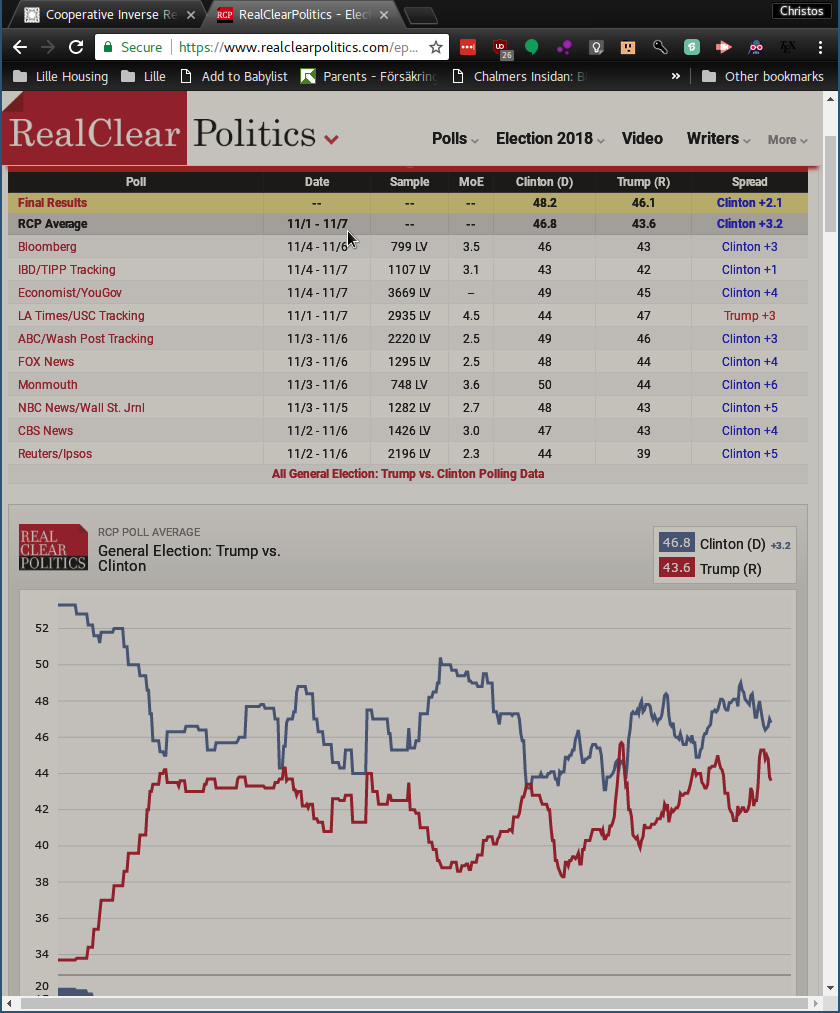
\includegraphics[width=\textwidth]{../figures/2016-election}}
\end{frame}

\subsection{Confidence intervals and $p$-values}
\begin{frame}
  \frametitle{The fallacy of $p$-values}
  \only<article>{A $p$-value has a uniform distribution under the null hypothesis. More precisely,let $x$ is our data and $H_0$ is our null hypothesis. If $H_0$ is true then $x \sim P_0$. Let}
  \[
    f(x) \tag{$p$-statistic}
  \]
  \only<article>{be a statistic on the data designed to have the property:}
  \[
    P_0(\cset{x}{f(x) \leq p}) = p.
  \]
  \only<article>{This ensures that the probability of rejecting the null hypothesis when it is true is actually $p$. But note that this is the definition of the uniform distribution, so $f(x)$ has a uniform distribution under $H_0$. Hence the value of $f(x)$ itself is uninformative. In theory we should simply choose $p$ before seeing the data and just accept or reject based on whether $f(x) \leq p$. However nobody does that in practice, meaning that $p$-values are used incorrectly. Better not to use them at all.}
\end{frame}


\begin{frame}
  \frametitle{Confidence intervals}
  \only<article>{Similarly, a confidence interval $I$ tells us the probability of an underlying value $\theta$ to be estimated being in $\theta \in I$, if our modelling assumption is correct.}
  \begin{block}[Confidence interval under a model $\mu$]
    \only<article>{
      The interval $I(\delta)$ for an estimator $\hat{\theta}$ of a parameter $\theta$ from data $x$ under the modelling assumptions $\mu$ is simply a set in $\Theta$ such that the true parameter lies in $I(\delta)$ with probability $1 - \delta$, i.e.
    }
    \[
      \Pr_\mu(\hat{\theta} \in I(\theta, \delta)) \geq 1 - \delta.
    \]
  \end{block}
  This is a property of the estimator $\hat{\theta} : \CX \to \Theta$ and tells us \emph{nothing direct} about our specific estimate $\hat{\theta(x)}$. \only<article>{It only tells that if we repeatedly apply this produre, we will only get an estimate outside of the interval a $\delta$-fraction of the time.}
\end{frame}

\subsection{Bayesian credible intervals}


\subsection{Model mismatch}

\subsection{Boot-strapping}

\subsection{Cross-validation}

\subsection{Independent replication}



%%% Local Variables:
%%% mode: latex
%%% TeX-master: "notes"
%%% End:

 


\begin{exercise}
  Work in teams of 2-3 students.

  Select an arbitrary classification dataset from \url{https://archive.ics.uci.edu/ml/datasets.html?task=cla}. 

  Select any arbitrary machine learning algorithm for classification
  from \texttt{scikitlearn} that can be used with this dataset, and identify its main hyperparameters.
    
  Varying at least one hyperparameter, use bootstrapping and/or
  cross-validation to find the optimal value for that hyperparameter,
  and report its performance. How close to the reported accuracy do
  you expect its performance to be in reality?  What are the factors
  that might cause it to deviate?
  
  Write a short report summarising both your methodology and your
  results. Exchange this report with another group of students. See
  whether you can reproduce exactly what they have done.
\end{exercise}

\section{Beliefs and probabilities}
\only<presentation>{
  \begin{frame}
    \tableofcontents[ 
    currentsection, 
    hideothersubsections, 
    sectionstyle=show/shaded
    ] 
  \end{frame}
}


\only<article>{Probability can be used to describe purely chance events, as in for example quantum physics. However, it is mostly used to describe uncertain events, such as the outcome of a dice roll or a coin flip, which only appear random. In fact, one can take it even further than that, and use it to model subjective uncertainty about any arbitrary event. Although probabilities are not the only way in which we can quantify uncertainty, it is a simple enough model, and with a rich enough history in mathematics, statistics, computer science and engineering that it is the most useful.}
\begin{frame}
  \frametitle{Uncertainty}
  \only<presentation>{
    \begin{itemize}
    \item We cannot perfectly predict the future.
    \item We cannot know for sure what happened in the past.
    \item How can we quantify this uncertainty?
    \item Probabilities!
    \end{itemize}
  }
  \only<artice>{
    \begin{definition}[$\sigma$-algebra]
      \index{$\sigma$-algebra}
      A $\sigma$-algebra $\Sigma$ on a set $\Omega$ has the following properties:
      \begin{enumerate}[(a)]
      \item $\Omega \in \Sigma$.
      \item If $A \in \Sigma$ then $A \subset \Omega$.
      \item If $A, B \in \Sigma$ then $A \cup B \in \Sigma$.
      \item If $A \in \Sigma$ then $\Omega \setminus A \in \Sigma$.
      \end{enumerate}
    \end{definition}
    For a more complete introduction to basic probability concepts, take a look at \citep[Appendix B]{dimitrakakis-ortner:dmuurl-book}, or \cite{degroot:optimalstatisticaldecisions}.
  }
  \begin{block}{Axioms of probability}
    \only<article>{Let $\Omega$ be the certain event, and $\Sigma$ is an appropriate $\sigma$-algebra on $\Omega$.}
    A probability measure $P$ on $(\Omega, \Sigma)$ has the following properties:
    \begin{enumerate}
    \item<2-> The probability of the certain event is $P(\Omega) = 1$
    \item<3->The probability of the impossible event is
      $P(\emptyset) = 0$
    \item<4->The probability of any event $A \in \Sigma$ is $0 \leq P(A) \leq 1$.
    \item<5-> If $A, B$ are disjoint, i.e. $A \cap B = \emptyset$, meaning
      that they cannot happen at the same time, then
      \[
      P(A \cup B) = P(A) + P(B)
      \]
    \end{enumerate}
  \end{block}
\end{frame}

\begin{frame}
  \only<article>{ Sometimes we would like to calculate the probability
    of some event $A$ happening given that we know that some other
    event $B$ has happened. For this we need to first define the idea
    of conditional probability.  }
  \begin{definition}[Conditional probability]
    The probability of $A$ happening if we know that $B$ has happened
    is defined to be:
    \[
    P(A \mid B) \defn \frac{P(A \cap B) }{P(B)}.
    \]
  \end{definition}
  \only<1>{
    Conditional probabilities obey the same rules as probabilities. }
  \only<article>{
    Here, the probability measure of any event $A$ given $B$ is defined to be the probability of the intersection of of the events divided by the second event.
    We can rewrite this definition as follows, by using the definition for $P(B \mid A)$}
  \begin{block}{Bayes's theorem}
    For $P(A_1 \cup A_2)  = 1$, $A_1 \cap A_2 = \emptyset$,
    \[
    P(A_i \mid B)
    \uncover<2->{= \frac{P(B \mid A_i) P(A_i)}{P(B)}}
    \uncover<3->{= \frac{P(B \mid A_i) P(A_i)}{P(B \mid A_1) P(A_1) + P(B \mid A_2) P(A_2)}}
    \]
  \end{block}
  \uncover<4->{
    \begin{example}[probability of rain]
      What is the probability of rain given a forecast $x_1$ or $x_2$?
      \begin{columns}
        \begin{column}{0.33\textwidth}
          \begin{table}[H]
            \centering
            \begin{tabular}{c|c}
              $\outcome_1$: rain & $P(\outcome_1) = 80\%$ \\
              $\outcome_2$: dry & $P(\outcome_2) = 20\%$
            \end{tabular}
            \caption{Prior probability of rain tomorrow}
          \end{table}
        \end{column}
        
        \begin{column}{0.33\textwidth}
          \uncover<5->{
            \begin{table}[H]
              \centering
              \begin{tabular}{c|c}
                $x_1$: rain & $P(x_1 \mid \outcome_1) = 90\%$ \\
                $x_2$: dry & $P(x_2 \mid \outcome_2) = 50\%$
              \end{tabular}
              \caption{Probability the forecast is correct}
            \end{table}
          }
        \end{column}
        \uncover<6->{
          \begin{column}{0.33\textwidth}
            \begin{table}[H]
              \centering
              \begin{tabular}{c}
                $P(\outcome_1 \mid x_1) = 87.8\%$ \\
                $P(\outcome_1 \mid x_2) = 44.4\%$
              \end{tabular}
              \caption{Probability that it will rain given the forecast}
            \end{table}
          }
        \end{column}
      \end{columns}
    \end{example}
  }
\end{frame}


\begin{frame}
  \frametitle{Classification in terms of conditional probabilities}
  \only<1>{
    \only<presentation>{
      \begin{itemize}
      \item Features $x_t \in \CX$.
      \item Class label $y_t \in \CY$.
      \item Probability model $P_\model(x_t \mid y_t)$.
      \item Prior class probability $P_\model(y_t = c)$.
      \end{itemize}
    }
  }
  \only<article>{
    Conditional probability naturally appears in classification problems. Given a new example vector of data $x_t \in \CX$, we would like to calculate the probability of different classes $c \in \CY$ given the data, $P_\model(y_t = c \mid x_t)$.  
    If we somehow obtained the distribution of data $P_\model(x_t \mid y_t)$ for each possible class, as well as the prior class probability $P_\model(y_t = c)$, 
    from Bayes's theorem, we see that we can obtain the probability of the class:
  }
  \only<1>{
    \[
    P_\model(y_t = c \mid x_t) = \frac{P_\model(x_t \mid y_t = c) P_\model(y_t = c)}{\sum_{c' \in \CY} P_\model(x_t \mid y_t = c') P_\model(y_t = c')}
    \]
  }
  \only<article>{
    for any class $c$. This directly gives us a method for classifying new data, as long as we have a way to obtain $P_\model(x_t \mid y_t)$ and $P_\model(y_t)$.
  }
  \only<1>{
    \begin{figure}[H]
      \centering
      \begin{tikzpicture}
        \node[RV] at (0,0) (x) {$y_t$};
        \node[RV] at (0,2) (y) {$x_t$};
        \node[RV] at (1,1) (m) {$\model$};
        \draw[->] (x) to (y);
        \draw[->] (m) to (x); \draw[->] (m) to (y);
      \end{tikzpicture}
      \caption{A generative classification model. $\model$ identifies the model (paramter). $x_t$ are the features and $y_t$ the class label of the $t$-th example.}
    \end{figure}
  }
  \begin{figure}[H]
    \centering
    \begin{subfigure}{\fwidth}
      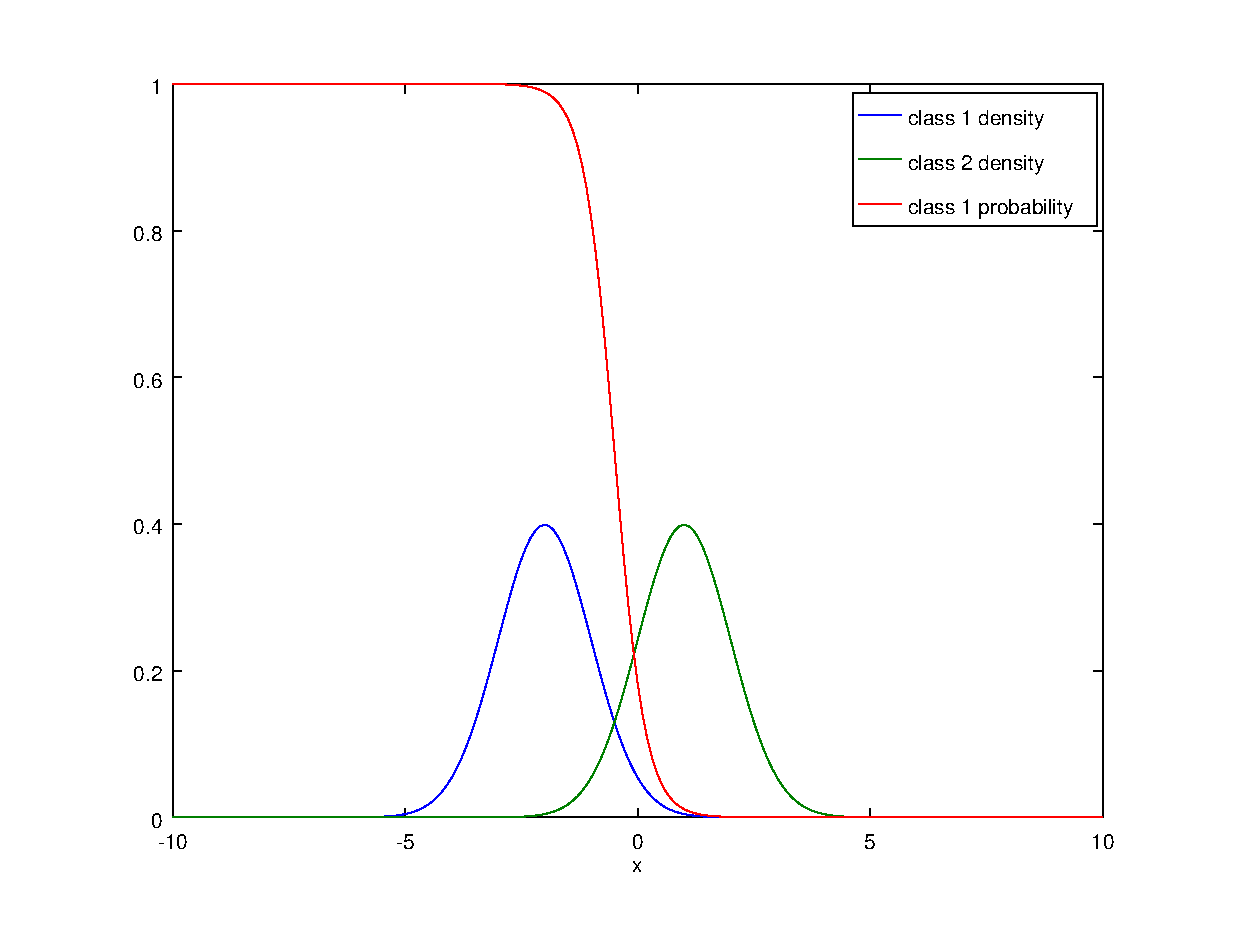
\includegraphics[width=\textwidth]{../figures/equal-variance}
      \caption{Equal prior and variance}
    \end{subfigure}
    \begin{subfigure}{\fwidth}
      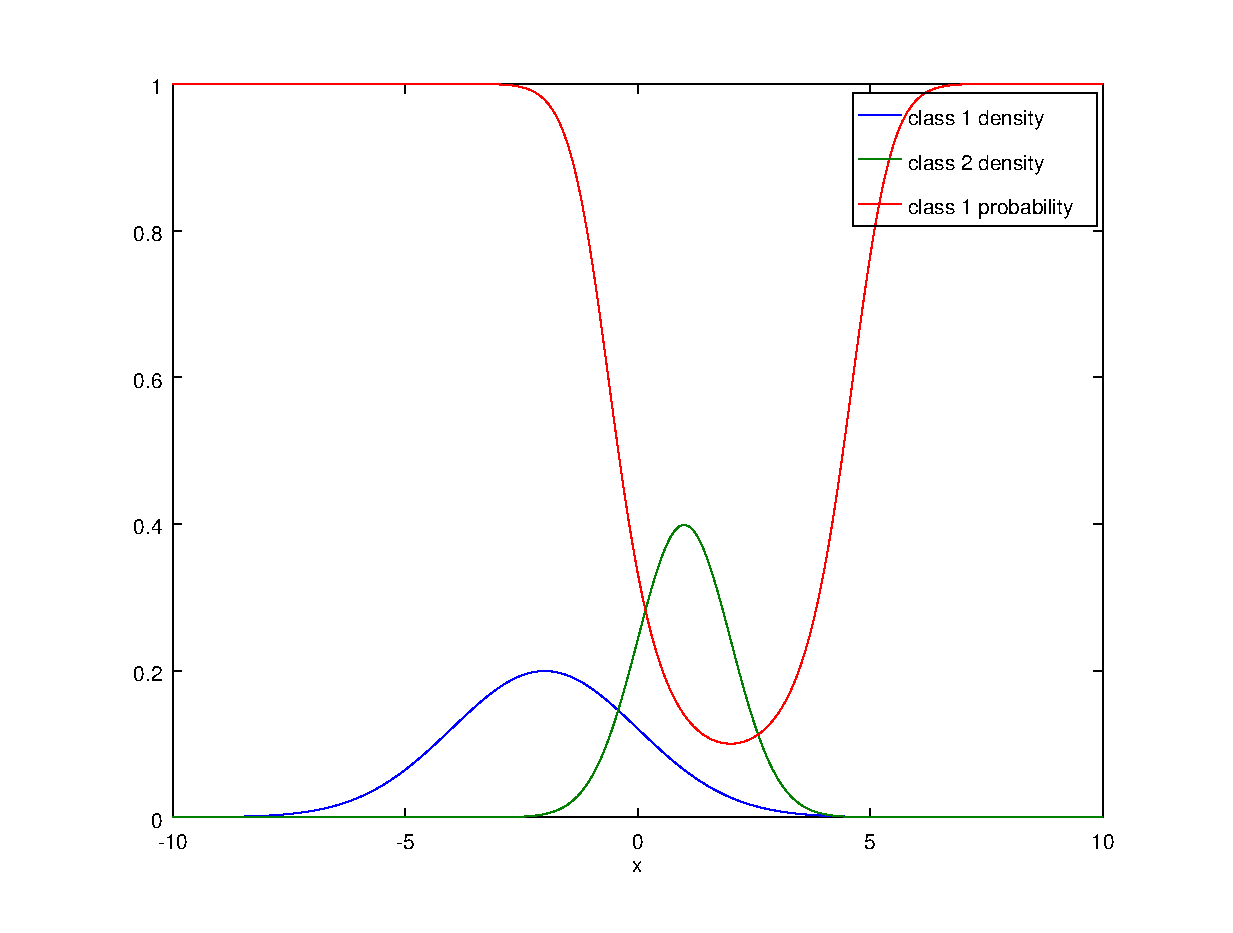
\includegraphics[width=\textwidth]{../figures/unequal-variance}
      \caption{Unequal variance}
    \end{subfigure}
    \begin{subfigure}{\fwidth}
      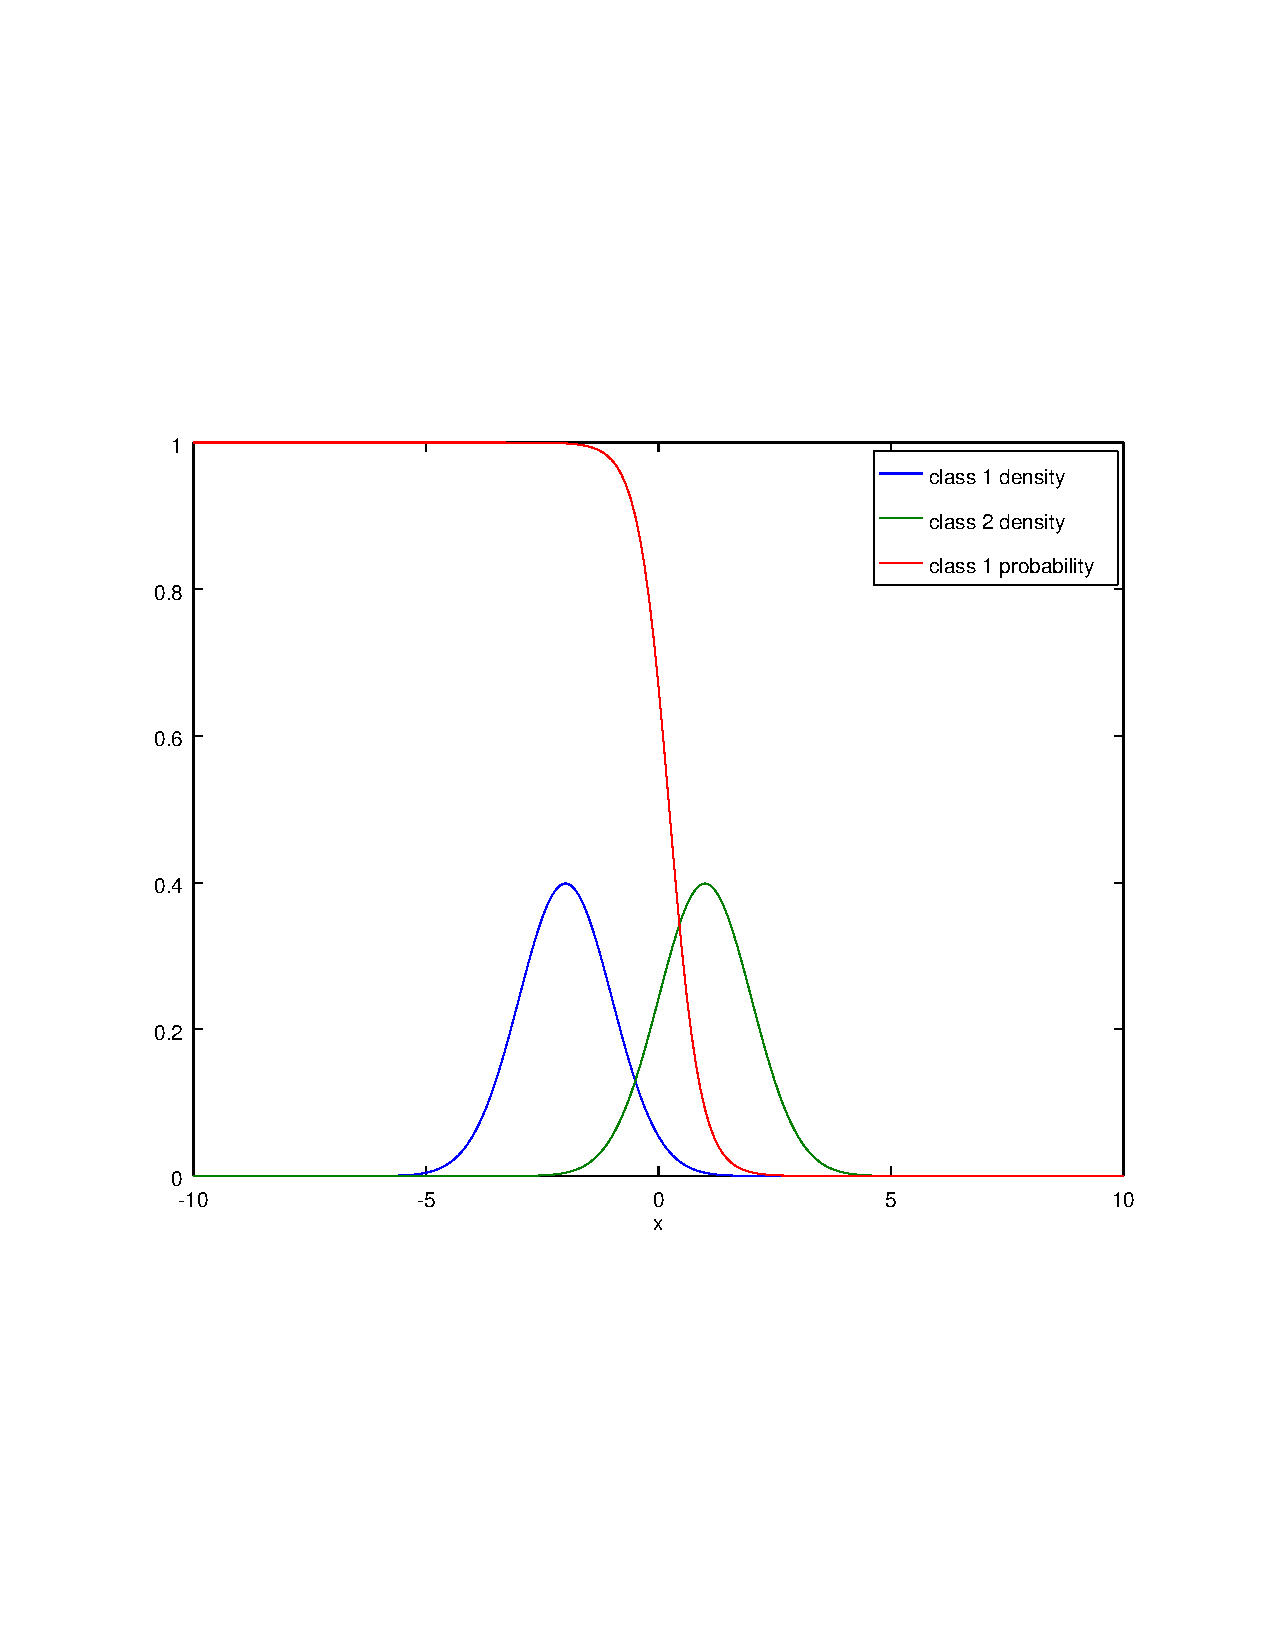
\includegraphics[width=\textwidth]{../figures/unequal-prior}
      \caption{Unequal prior}
    \end{subfigure}
    \caption{The effect of changing variance and prior on the classification decision when we assume a normal distribution.}
    \label{fig:normal-generative}
  \end{figure}
  \begin{example}[Normal distribution]
    A simple example is when $x_t$ is normally distributed in a matter that depends on the class.  Figure~\ref{fig:normal-generative} shows the distribution of $x_t$ for two different classes, with means of $-1$ and $+1$ respectively, for three different case. In the first case, both classes have variance of 1, and we assume the same prior probability for both
    \[
    x_t \mid y_t = 0 \sim \Normal(-1,1),
    \qquad
    x_t \mid y_t = 1 \sim \Normal(1,1)
    \]
    \[
    x_t \mid y_t = 0 \sim \Normal(-1,1),
    \qquad
    x_t \mid y_t = 1 \sim \Normal(1,1)
    \]

  \end{example}
  
  \uncover<5>{
    \alert{But how can we get a probability model in the first place?}
  }
\end{frame}


\begin{frame}
  \frametitle{Subjective probability}
  \only<article>{While probabilities apply to truly random events, they are also useful for representing subjective uncertainty. In this course, we will use a special symbol for subjective probability, $\bel$.}
  \begin{block}{Subjective probability measure $\bel$}
    \begin{itemize}
    \item If we think event $A$ is more likely than $B$, then $\bel(A) > \bel(B)$.
    \item Usual rules of probability apply:
      \begin{enumerate}
      \item $\bel(A) \in [0,1]$.
      \item $\bel(\emptyset) = 0$.
      \item If $A \cap B = \emptyset$, then $\bel(A \cup B) = \bel(A) + \bel(B)$.
      \end{enumerate}
    \end{itemize}
  \end{block}
\end{frame}


\begin{frame}
  \frametitle{Bayesian inference illustration}
  \begin{columns}
    \begin{column}{0.7\textwidth}
      \begin{block}{Use a subjective belief $\bel(\model)$ on $\Model$}
        \begin{itemize}
        \item<1-> \alert{Prior} belief $\bel(\model)$ represents our initial uncertainty.
        \item<2-> We \alert{observe history} $h$.
        \item<3->Each possible $\model$ assigns a \alert{probability} $P_\model(h)$ to $h$.
        \item<4-> We can use this to \alert{update} our belief via Bayes' theorem to obtain the \alert{posterior} belief:
          \[
          \bel(\model \mid h) \propto P_\model(h) \bel(\model)
          \tag{conclusion = evidence $\times$ prior}
          \]
        \end{itemize}
      \end{block}
    \end{column}
    \begin{column}{0.3\textwidth}
      \centering
      \uncover<1->{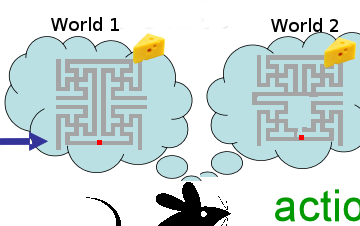
\includegraphics[width=0.5\fwidth]{../figures/rl_worlds}
        \\
        prior
      }
      \\
      \uncover<2->{
\includegraphics[width=0.5\fwidth]{../figures/rl_observations}
        \\
        evidence
      }
      \\
      \uncover<4->{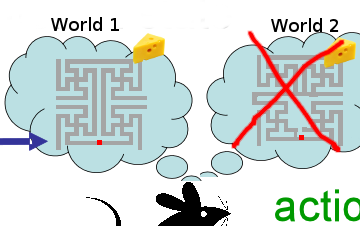
\includegraphics[width=0.5\fwidth]{../figures/rl_worlds2}
        \\ 
        conclusion
      }
    \end{column}
  \end{columns}
\end{frame}




\subsection{Probability and Bayesian inference}
\only<article>{One of the most important methods in machine learning
  and statistics is that of Bayesian inference.  This is the most
  fundamental method of drawing conclusions from data and explicit
  prior assumptions. In Bayesian inference, prior assumptions are
  represented as a probabilities on a space of hypotheses. Each
  hypothesis is seen as a probabilistic model of all possible data
  that we can see.}

\only<article>{Frequently, we want to draw conclusions from data. However, the conclusions are never solely inferred from data, but also depend on prior assumptions about reality.}




\begin{frame}
  \frametitle{Some examples}

  \begin{example}
    John claims to be a medium. He throws a coin $n$ times and predicts its value always correctly. Should we believe that he is a medium?
    \begin{itemize}
    \item $\model_1$: John is a medium.
    \item $\model_0$: John is not a medium.
    \end{itemize}
  \end{example}
  The answer depends on what we \alert{expect} a medium to be able to do, and how likely we thought he'd be a medium in the first place.

  \only<article>{
    \begin{example}
      Traces of DNA are found at a murder scene. We perform a DNA test against a database of $10^4$ citizens registered to be living in the area. We know that the probability of a false positive (that is, the test finding a match by mistake) is $10^{-6}$. If there is a match in the database, does that mean that the citizen was at the scene of the crime?
    \end{example}
  }
\end{frame}





\begin{frame}
  \frametitle{Bayesian inference}
  \only<article>{
    Now let us apply this idea to our specific problem. We already have the probability of the observation for each model, but we just need to define a \emph{prior probability} for each model. Since this is usually completely subjective, we give it another symbol.
  }
  \only<article>{
    \begin{block}{Prior probability}
      The prior probability $\bel$ on a set of models $\Model$ specifies our subjective belief $\bel(\model)$ that each model is true.\footnote{More generally $\bel$ is a probability measure.}
    \end{block}
  }
  \only<article>{
    This allows us to calculate the probability of John being a medium, given the data:
    \[
    \bel(\model_1 \mid \bx) = \frac{\Pr(\bx \mid \model_1) \bel(\model_1)}{\Pr_\bel(\bx)},
    \]
    where
    \[
    \Pr_\bel(\bx) \defn \Pr(\bx \mid \model_1) \bel(\model_1) + \Pr(\bx \mid \model_0) \bel(\model_0).
    \]
    The only thing left to specify is $\bel(\model_1)$, the probability that John is a medium before seeing the data. This is our subjective prior belief that mediums exist and that John is one of them.
    More generally, we can think of Bayesian inference as follows: }
  \begin{itemize}
  \item<1-> \only<article>{We start with a set of } mutually exclusive models $\Model = \{\model_1, \ldots, \model_k\}$.
  \item<2->\only<article>{Each model $\model$ is represented by a specific probabilistic model for any possible data $x$, that is}
    \only<presentation>{Probability model for any data $x$:} $P_\model(x) \equiv \Pr(x \mid \model)$.
  \item<3-> For each model, we have a prior probability $\bel(\model)$ that it is correct.
  \item<4-> \only<article>{After observing the data, we can calculate a posterior probability that the model is correct:}
    \only<presentation>{Posterior probability}
    \[
    \bel(\model \mid x) = \frac{\Pr(x \mid \model) \bel(\model)}{\sum_{\model' \in \Model} \Pr(x \mid \model') \bel(\model')}
    = \frac{P_\model(x) \bel(\model)}{\sum_{\model' \in \Model} P_{\model'} (x) \bel(\model')}.
    \]
  \end{itemize}
  \only<5->{
    \begin{block}{Interpretation}
      \begin{itemize}
      \item $\CM$: Set of all possible models that could describe the data.
      \item $P_\model(x)$: Probability of $x$ under model $\model$.
      \item Alternative notation $\Pr(x \mid \model)$: Probability of $x$ given that model $\model$ is correct.
      \item $\bel(\model)$: Our belief, before seeing the data, that $\model$ is correct.
      \item $\bel(\model \mid x)$: Our belief, aftering seeing the data, that $\model$ is correct.
      \end{itemize}
    \end{block}
    \only<article>{It must be emphasized that $P_\model(x) = \Pr(x \mid \model)$ as they are simply two different notations for the same thing. In words the first can be seen as the probability that model $\model$ assigns to data $x$, while the second as the probability of $x$ if $\model$ is the true model.}
  }
  \only<article>{
    Combining the prior belief with evidence is key in this procedure. Our posterior belief can then be used as a new prior belief when we get more evidence.}
\end{frame}
\begin{frame}
  \begin{exercise}[Continued example for medium]
    \only<article>{ Now let us apply this idea to our specific
      problem. We first make an independence assumption. In particular, we can assume that success and failure comes from a Bernoulli distribution with a parameter depending on the model.}
    \begin{align}
      P_{\model} (x) &= \prod_{t=1}^n P_{\model} (x_t).
                       \tag{independence property}
    \end{align}
    \only<article>{We first need to specify how well a medium could predict. Let's assume that a true medium would be able to predict perfectly, and that a non-medium would only predict randomly. This leads to the following models:}
    \begin{align}
      P_{\model_1}(x_t = 1) &= 1, &P_{\model_1}(x_t = 0) &= 0.
                                                           \tag{true medium model}
      \\
      P_{\model_0}(x_t = 1) &= 1/2, &P_{\model_0}(x_t = 0) &= 1/2.
                                                             \tag{non-medium model}
    \end{align}
    \only<article>{
      The only thing left to specify is $\bel(\model_1)$, the probability
      that John is a medium before seeing the data. This is our
      subjective prior belief that mediums exist and that John is one of
      them.}
    \uncover<3->{
      \begin{align}
        \bel(\model_0) &= 1/2,   &  \bel(\model_1) &= 1/2.
                                                     \tag{prior belief}
      \end{align}
    }
    \only<article>{Combining the prior belief with evidence is key in this
      procedure. Our posterior belief can then be used as a new prior
      belief when we get more evidence.  }
    \uncover<4>{
      \begin{align}
        \bel(\model_1 \mid x) & = \frac{P_{\model_1}(x)
                                \bel(\model_1)}{\Pr_\bel(x)} \tag{posterior belief}
        \\
        \Pr_\bel(x) &\defn P_{\model_1}(x) \bel(\model_1) + P_{\model_0}(x) \bel(\model_0).
                      \tag{marginal distribution}
      \end{align}
    }
    Throw a coin 4 times, and have a classmate make a prediction. What your belief that your classmate is a medium? Is the prior you used reasonable?
  \end{exercise}
\end{frame}


\begin{frame}
  \frametitle{Sequential update of beliefs}
  \only<article>{Assume you have $n$ meteorologists. At each day $t$, each meteorologist $i$ gives a probability $p_{t,\model_i}\defn P_{\model_i}(x_t = \textrm{rain})$ for rain. Consider the case of there being three meteorologists, and each one making the following prediction for the coming week. Start with a uniform prior $\bel(\model) = 1/3$ for each model.}
  {
    \begin{table}[h]
      \begin{tabular}{c|l|l|l|l|l|l|l}
        &M&T&W&T&F&S&S\\
        \hline
        CNN & 0.5 & 0.6 & 0.7 & 0.9 & 0.5 & 0.3 & 0.1\\
        SMHI & 0.3 & 0.7 & 0.8 & 0.9 & 0.5 & 0.2 & 0.1\\
        YR & 0.6 & 0.9 & 0.8 & 0.5 & 0.4 & 0.1 & 0.1\\
        \hline
        Rain? & Y & Y & Y & N & Y & N & N
      \end{tabular}
      \caption{Predictions by three different entities for the probability of rain on a particular day, along with whether or not it actually rained.}
      \label{tab:meteorologists}
    \end{table}
  }
  \begin{exercise}
    \begin{itemize}
    \item $n$ meteorological stations $\cset{\mdp_i}{i=1, \ldots,n}$
    \item The $i$-th station predicts rain $P_{\mdp_i}(x_t \mid x_1, \ldots, x_{t-1})$.
    \item Let $\bel_t(\mdp)$ be our belief at time $t$.
      Derive the next-step belief
      $\bel_{t+1}(\mdp) \defn  \bel_t(\mdp | y_{t})$ in terms of the current belief $\bel_t$.
    \item Write a python function that computes this posterior
    \end{itemize}
  \end{exercise}
  \uncover<2->{
    \[
    \bel_{t+1}(\mdp)
    \defn
    \bel_t(\mdp | x_{t})
    =
    \frac{P_\mdp(x_t \mid x_1, \ldots, x_{t-1}) \bel_t(\mdp)}
    {\sum_{\mdp'} P_{\mdp'}(x_t \mid x_1, \ldots, x_{t-1}) \bel_t(\mdp')}
    \]
  }
\end{frame}



\begin{frame}[label=beta-example]
  \frametitle{Bayesian inference for Bernoulli distributions}
  \only<1>{
    \begin{block}{Estimating a coin's bias}
      A fair coin comes heads $50\%$ of the time. 
      We want to test an unknown coin, which we think may not be completely fair. 
    \end{block}
  }
  \only<1,2>{
    \begin{figure}[h]
      \centering
      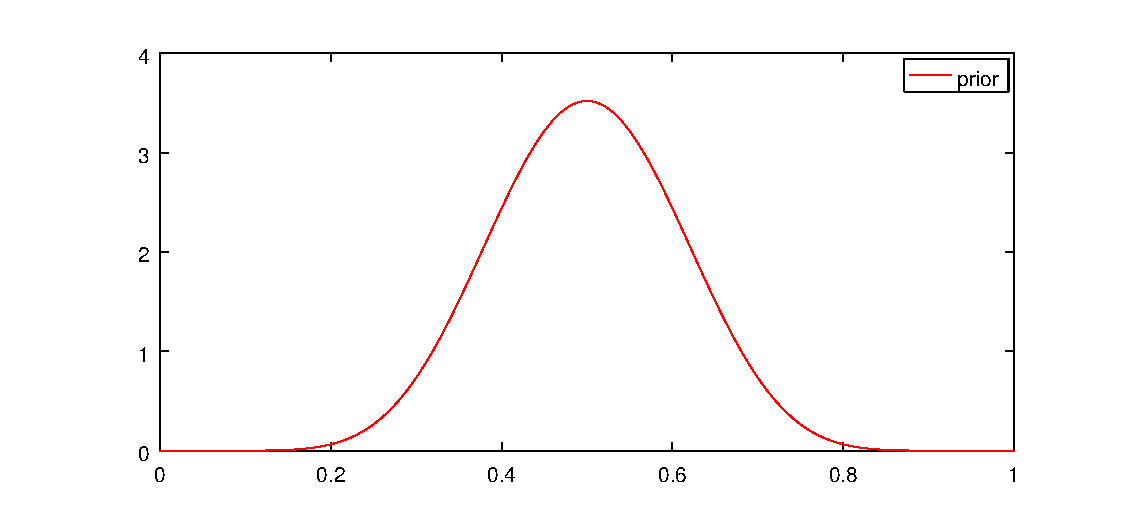
\includegraphics[width=\textwidth]{../figures/beta-prior}
      \caption{Prior belief $\bel$ about the coin bias $\theta$.}
    \end{figure}
  }
  \only<2>{
    For a sequence of throws $x_t \in \{0,1\}$,
    \[
    P_\theta(x) \propto \prod_t \theta^{x_t} (1 - \theta)^{1 - x_t}
    = \theta^{\textrm{\#Heads}} (1 - \theta)^{\textrm{\#Tails}}
    \]
  }
  \only<3>{
    \begin{figure}[h]
      \centering
      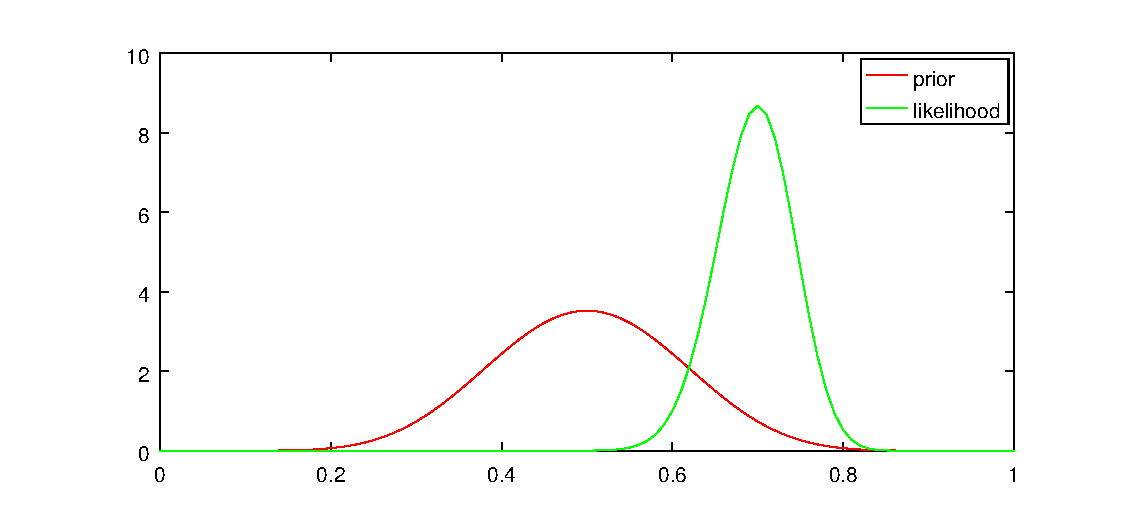
\includegraphics[width=\textwidth]{../figures/beta-likelihood}
      \caption{Prior belief $\bel$ about the coin bias $\theta$ and likelihood of $\theta$ for the data.}
    \end{figure}
    Say we throw the coin 100 times and obtain 70 heads. Then we plot the \alert{likelihood} $P_\theta(x)$ of different models.
  }
  \only<4>{
    \begin{figure}[h]
      \centering
      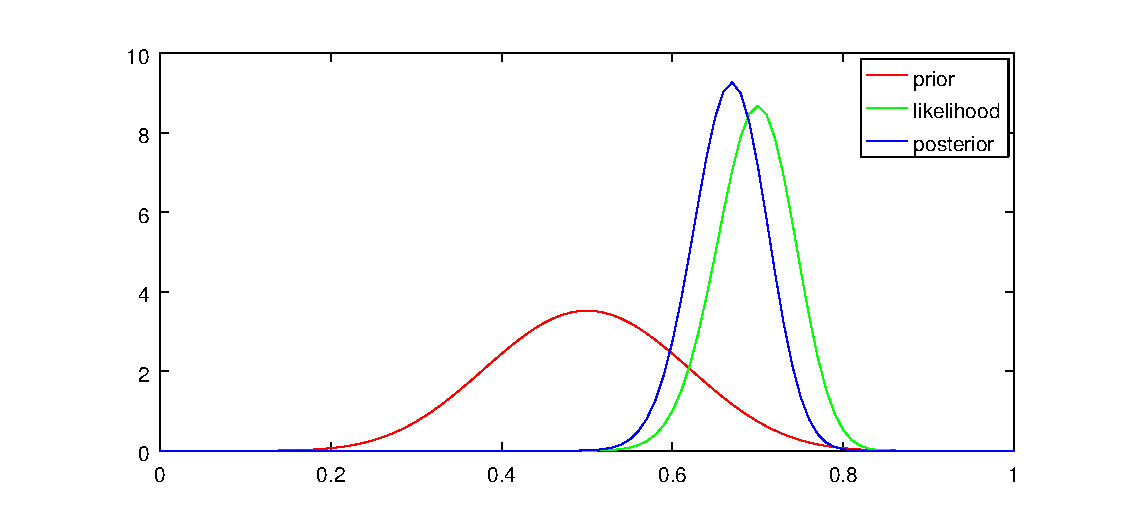
\includegraphics[width=\textwidth]{../figures/beta-posterior}
      \caption{Prior belief $\bel(\theta)$ about the coin bias $\theta$, likelihood of $\theta$ for the data, and posterior belief $\bel(\theta \mid x)$}
    \end{figure}
    From these, we calculate a \alert{posterior} distribution over the correct models. This represents our conclusion given our prior and the data.
  }
  \only<article>{If the prior distribution is described by the so-called Beta density
    \[
    f(\theta \mid \alpha, \beta) \propto \theta^{\alpha -1} (1 - \theta)^{\beta -1}
    \]
    where $\alpha, \beta$ describe the shape of the Beta distribution.
  }
\end{frame}

\subsubsection{Riemann and Lebesgue integrals}
\only<article>{
  Since $\bel$ is a probability measure over models $\Param$, it is always simple to write the posterior probability given some data $x$ in the following terms when $\Param$ is discrete (finite or countable):
  \[
  \bel(\param \mid x) = \frac{P_\param(x) \bel(\param)}{\sum_{\param'} P_{\param'(x) \bel(\param')}.}
  \]
  However, in many situations $\Param$ is uncountable, i.e. $\Param \subset \Reals^k$. Then, as both the prior $\bel$ and the posterior $\bel(\cdot \mid x)$ have to be probability measures on $\Param$, they are defined over subsets of $\Param$. This means that we can write the posterior in terms of Lebesgue integrals:
  \[
  \bel(B \mid x) = \frac{\int_B P_\param(x) \dd \bel(\param)}{\int_\Param P_\param(x) \dd \bel(\param)}.
  \]
  Alternatively, we can abuse notation and use $\bel(\param)$ to describe a density, so that the \emindex{posterior density} is written in terms of a Riemann integral:
  \[
  \bel(\param \mid x) \defn \frac{P_\param(x) \bel(\param) \dd \param}{\int_{\Param} P_{\param'}(x) \bel(\param') \param'}.
  \]
  However, the advantage of the Lebesgue integral notation is that it works the same no matter whether $\Param$ is discrete or continuous.
}
\begin{frame}
  \frametitle{Learning outcomes}
  \begin{block}{Understanding}
    \begin{itemize}
    \item The axioms of probability, marginals and conditional distributions.
    \item The philosophical underpinnings of Bayesianism.
    \item The simple conjugate model for Bernoulli distributions.
    \end{itemize}
  \end{block}
  
  \begin{block}{Skills}
    \begin{itemize}
    \item Be able to calculate with probabilities using the marginal and conditional definitions and Bayes rule.
    \item Being able to implement a simple Bayesian inference algorithm in Python.
    \end{itemize}
  \end{block}

  \begin{block}{Reflection}
    \begin{itemize}
    \item How useful is the Bayesian representation of uncertainty?
    \item How restrictive is the need to select a prior distribution?
    \item Can you think of another way to explicitly represent uncertainty in a way that can incorporate new evidence?
    \end{itemize}
  \end{block}
  
\end{frame}

%%% Local Variables:
%%% mode: latex
%%% TeX-engine: xetex
%%% TeX-master: "notes.tex"
%%% End:
 % Bayesian inference
\section{Hierarchies of decision making problems}
\only<presentation>{
  \begin{frame}
    \tableofcontents[ 
    currentsection, 
    hideothersubsections, 
    sectionstyle=show/shaded
    ] 
  \end{frame}
}


\only<article>{
  All machine learning problems are essentially decision problems. This essentially means replacing some human decisions with machine decisions. One of the simplest decision problems is classification, where you want an algorithm to decide the correct class of some data, but even within this simple framework there is a multitude of decisions to be made. The first is how to frame the classification problem the first place. The second is how to collect, process and annotate the data. The third is choosing the type of classification model to use. The fourth is how to use the collected data to find an optimal classifier within the selected type. After all this has been done, there is the problem of classifying new data. In this course, we will take a holistic view of the problem, and consider each problem in turn, starting from the lowest level and working our way up.}


\subsection{Simple decision problems}
\begin{frame}
  \frametitle{Preferences}
  \only<article>{The simplest decision problem involves selecting one item from a set of choices, such as in the following examples}  
  \begin{example}
    \begin{block}{Food}
      \begin{itemize}
      \item[A] McDonald's cheeseburger
      \item[B] Surstromming
      \item[C] Oatmeal
      \end{itemize}
    \end{block}
    \begin{block}{Money}
      \begin{itemize}
      \item[A] 10,000,000 SEK
      \item[B] 10,000,000 USD
      \item[C] 10,000,000 BTC
      \end{itemize}
    \end{block}
    \begin{block}{Entertainment}
      \begin{itemize}
      \item[A] Ticket to Liseberg
      \item[B] Ticket to Rebstar
      \item[C] Ticket to Nutcracker
      \end{itemize}
    \end{block}
  \end{example}
\end{frame}

\begin{frame}
  \frametitle{Rewards and utilities}
  \only<article>{In the decision theoretic framework, the things we receive are called rewards, and we assign a utility value to each one of them, showing which one we prefer.}
  \begin{itemize}
  \item Each choice is called a \alert{reward} $r \in \CR$.
  \item There is a \alert{utility function} $U : \CR \to \Reals$, assigning values to reward.
  \item We (weakly) prefer $A$ to $B$ iff $U(A) \geq U(B)$.
  \end{itemize}
  \only<article>{In each case, given $U$ the choice between each reward is trivial. We just select the reward:
    \[
      r^* \in \argmax_r U(r)
    \]
    The main difficult is actually selecting the appropriate utility function. In a behavioural context, we simply assume that humans act with respect to a specific utility function. However, figuring out this function from behavioural data is non trivial. ven when this assumption is correct, individuals do not have a common utility function.
  }
  \begin{exercise}
    From your individual preferences, derive a \alert{common utility function} that reflects everybody's preferences in the class for each of the three examples. Is there a simple algorithm for deciding this? Would you consider the outcome fair?
  \end{exercise}
\end{frame}

\begin{frame}
  \frametitle{Preferences among random outcomes}
  \begin{example}
    Would you rather \ldots
    \begin{itemize}
    \item[A] Have 100 EUR now?
    \item[B] Flip a coin, and get 200 EUR if it comes heads?
    \end{itemize}    
  \end{example}
  \uncover<2->{
    \begin{block}{The expected utility hypothesis}
      Rational decision makers prefer choice $A$ to $B$ if
      \[
        \E(U | A) \geq \E(U | B),
      \]
      where the expected utility is
      \[
        \E(U | A) = \sum_r U(r) \Pr(r | A).
      \]
    \end{block}
    In the above example, $r \in \{0, 100, 200\}$ and $U(r)$ is
    increasing, and the coin is fair.
  }
  \begin{itemize}
  \item<3-> If $U$ is convex, we prefer B.
  \item<4-> If $U$ is concave, we prefer A.
  \item<5-> If $U$ is linear, we don't care.
  \end{itemize}
\end{frame}


\begin{frame}
  \frametitle{Uncertain rewards}
  \only<article>{However, in real life, there are many cases where we can only choose between uncertain outcomes. The simplest example are lottery tickets, where rewards are essentially random. However, in many cases the rewards are not really random, but simply uncertain. In those cases it is useful to represent our uncertainty with probabilities as well, even though there is nothing really random.}
  \begin{itemize}
  \item Decisions $\decision \in \Decision$
  \item Each choice is called a \alert{reward} $r \in \CR$.
  \item There is a \alert{utility function} $U : \CR \to \Reals$, assigning values to reward.
  \item We (weakly) prefer $A$ to $B$ iff $U(A) \geq U(B)$.
  \end{itemize}

  \begin{example}
    \begin{columns}
      \begin{column}{0.5\textwidth}
        You are going to work, and it might rain.  What do you do?
        \begin{itemize}
        \item $\decision_1$: Take the umbrella.
        \item $\decision_2$: Risk it!
        \item $\outcome_1$: rain
        \item $\outcome_2$: dry
        \end{itemize}
      \end{column}
      \begin{column}{0.5\textwidth}
        \begin{table}
          \centering
          \begin{tabular}{c|c|c}
            $\Rew(\outcome,\decision)$ & $\decision_1$ & $\decision_2$ \\ %ro: U has only one argument.
            \hline
            $\outcome_1$ & dry, carrying umbrella & wet\\
            $\outcome_2$ & dry, carrying umbrella & dry\\
            \hline
            \hline
            $U[\Rew(\outcome,\decision)]$ & $\decision_1$ & $\decision_2$ \\
            \hline
            $\outcome_1$ & 0 & -10\\
            $\outcome_2$ & 0 & 1
          \end{tabular}
          \caption{Rewards and utilities.}
          \label{tab:rain-utility-function}
        \end{table}

        \begin{itemize}
        \item<2-> $\max_\decision \min_\outcome U = 0$
        \item<3-> $\min_\outcome \max_\decision U = 0$
        \end{itemize}
      \end{column}

    \end{columns}
  \end{example}
\end{frame}



\begin{frame}
  \frametitle{Expected utility}
  \[
    \E (U \mid a) = \sum_r U[\Rew(\outcome, \decision)] \Pr(\outcome \mid \decision)
  \]
  \begin{example}%ro: rather an exercise?
    You are going to work, and it might rain. The forecast said that
    the probability of rain $(\outcome_1)$ was $20\%$. What do you do?
    \begin{itemize}
    \item $\decision_1$: Take the umbrella.
    \item $\decision_2$: Risk it!
    \end{itemize}
    \begin{table}
      \centering
      \begin{tabular}{c|c|c}
        $\Rew(\outcome,\decision)$ & $\decision_1$ & $\decision_2$ \\ %ro: U has only one argument.
        \hline
        $\outcome_1$ & dry, carrying umbrella & wet\\
        $\outcome_2$ & dry, carrying umbrella & dry\\
        \hline
        \hline
        $U[\Rew(\outcome,\decision)]$ & $\decision_1$ & $\decision_2$ \\
        \hline
        $\outcome_1$ & 0 & -10\\
        $\outcome_2$ & 0 & 1\\
        \hline
        \hline
        $\E_P(U \mid \decision)$ & 0 &  -1.2 \\ 
      \end{tabular}
      \caption{Rewards, utilities, expected utility for $20\%$ probability of rain.}
      \label{tab:rain-utility-function}
    \end{table}
  \end{example}
\end{frame}





\subsection{Decision rules}

\only<article>{We now move from simple decisions to decisions that
  depend on some observation. We shall start with a simple problem in applied meteorology. Then we will discuss hypothesis testing as a decision making problem. Finally, we will go through an exercise in Bayesian methods for classification.}

\begin{frame}
  \frametitle{Bayes decision rules}
  Consider the case where outcomes are independent of decisions:
  \[
    \util (P, \decision) \defn \sum_{\model}  \util (\model, \decision) P(\model)
  \]
  This corresponds e.g. to the case where $P(\omega)$ is the belief about an unknown world.
  \begin{definition}[Bayes utility]
    \label{def:bayes-utility}
    The maximising decision for $P$ has an expected utility equal to:
    \begin{equation}
      \BUtil(P) \defn \sup_{\decision \in \Decision} \util (P, \decision).
      \label{eq:bayes-utility}
    \end{equation}
  \end{definition}
\end{frame}




\begin{frame}
  \frametitle{The $n$-meteorologists problem}
  \only<article>{Of course, we may not always just be interested in classification performance in terms of predicting the most likely class. It strongly depends on the problem we are actually wanting to solve. In  biometric authentication, for example, we want to guard against the unlikely event that an impostor will successfully be authenticated. Even if the decision rule that always says 'OK' has the lowest classification error in practice, the expected cost of impostors means that the optimal decision rule must sometimes say 'Failed' even if this leads to false rejections sometimes.}
  \begin{exercise}
    \only<presentation>{
      \only<1>{
        \begin{itemize}
        \item Meteorological models $\CM = \set{\model_1, \ldots, \model_n}$
        \item Rain predictions at time $t$: $p_{t,\model} \defn  P_{\model}(x_t = \textrm{rain})$.
        \item Prior probability $\bel(\model) = 1/n$ for each model.
        \item Should we take the umbrella?
        \end{itemize}
      }
    }
    \only<article>{Assume you have $n$ meteorologists. At each day $t$, each meteorologist $i$ gives a probability $p_{t,\model_i}\defn P_{\model_i}(x_t = \textrm{rain})$ for rain. Consider the case of there being three meteorologists, and each one making the following prediction for the coming week. Start with a uniform prior $\bel(\model) = 1/3$ for each model.}
    {
      \begin{table}[h]
        \begin{tabular}{c|l|l|l|l|l|l|l}
          &M&T&W&T&F&S&S\\
          \hline
          CNN & 0.5 & 0.6 & 0.7 & 0.9 & 0.5 & 0.3 & 0.1\\
          SMHI & 0.3 & 0.7 & 0.8 & 0.9 & 0.5 & 0.2 & 0.1\\
          YR & 0.6 & 0.9 & 0.8 & 0.5 & 0.4 & 0.1 & 0.1\\
          \hline
          Rain? & Y & Y & Y & N & Y & N & N
        \end{tabular}
        \caption{Predictions by three different entities for the probability of rain on a particular day, along with whether or not it actually rained.}
        \label{tab:meteorologists}
      \end{table}
    }
    \uncover<2->{
      \begin{enumerate}
      \item<2-> What is your belief about the quality of each meteorologist after each day? 
      \item<3-> What is your belief about the probability of rain each day? 
        \[
          P_\bel(x_t = \textrm{rain} \mid x_1, x_2, \ldots x_{t-1})
          =
          \sum_{\model \in \Model} P_\model(x_t = \textrm{rain})
          \bel(\model \mid x_1, x_2, \ldots x_{t-1}) 
        \]
      \item<4-> Assume you can decide whether or not to go running each
        day. If you go running and it does not rain, your utility is 1. If
        it rains, it's -10. If you don't go running, your utility is
        0. What is the decision maximising utility in expectation (with respect to the posterior) each
        day?
      \end{enumerate}
    }
  \end{exercise}
\end{frame}


\subsection{Statistical testing}
\only<article>{A common type of decision problem is a statistical test. This arises when we have a set of possible candidate models $\CM$ and we need to be able to decide which model to select after we see the evidence.
  Many times, there is only one model under consideration, $\model_0$, the so-called \alert{null hypothesis}. Then, our only decision is whether or not to accept or reject this hypothesis.}
\begin{frame}
  \frametitle{Simple hypothesis testing}
  \only<article>{Let us start with the simple case of needing to compare two models.}
  \begin{block}{The simple hypothesis test as a decision problem}
    \begin{itemize}
    \item $\CM = \{\model_0, \model_1\}$
    \item $a_0$: Accept model $\model_0$
    \item $a_1$: Accept model $\model_1$
    \end{itemize}
    \begin{table}[H]
      \begin{tabular}{c|cc}
        $\util$& $\model_0$& $\model_1$\\\hline
        $a_0$ & 1 & 0\\
        $a_1$ & 0 & 1
      \end{tabular}
      \caption{Example utility function for simple hypothesis tests.}
    \end{table}
    \only<article>{There is no reason for us to be restricted to this utility function. As it is diagonal, it effectively treats both types of errors in the same way.}
  \end{block}

  \begin{example}[Continuation of the medium example]
    \begin{itemize}
    \item $\model_1$: that John is a medium.
    \item $\model_0$: that John is not a medium.
    \end{itemize}
    \only<article>{
    Let $x_t$ be $0$ if John makes an incorrect prediction at time $t$ and $x_t = 1$ if he makes a correct prediction. Let us once more assume a Bernoulli model, so that John's claim that he can predict our tosses perfectly means that for a sequence of tosses $\bx = x_1, \ldots, x_n$,
    \[
      P_{\model_1}(\bx) = \begin{cases}
        1, & x_t = 1 \forall t \in [n]\\
        0, & \exists t \in [n] : x_t = 0.
      \end{cases}
    \]
    That is, the probability of perfectly correct predictions is 1, and that of one or more incorrect prediction is 0. For the other model, we can assume that all draws are independently and identically distributed from a fair coin. Consequently, no matter what John's predictions are, we have that:
    \[
      P_{\model_0}(\bx = 1 \ldots 1) = 2^{-n}.
    \]
    So, for the given example, as stated, we have the following facts:
    \begin{itemize}
    \item If John makes one or more mistakes, then $\Pr(\bx \mid \model_1) = 0$ and $\Pr(\bx \mid \model_0) = 2^{-n}$. Thus, we should perhaps say that then John is not a medium
    \item If John makes no mistakes at all, then 
      \begin{align}
        \Pr(\bx = 1, \ldots, 1 \mid \model_1) &= 1,
        &
          \Pr(\bx = 1, \ldots, 1 \mid \model_0) &= 2^{-n}.
      \end{align}
    \end{itemize}
    Now we can calculate the posterior distribution, which is
    \[
      \bel(\model_1 \mid \bx = 1, \ldots, 1) = \frac{1 \times \bel(\model_1)}{1 \times \bel(model_1) + 2^{-n} (1 - \bel(\model_1))}.
    \]
    Our expected utility for taking action $a_0$ is actually
  }
  \[
    \E_\bel(\util \mid a_0) = 1 \times \bel(\model_0 \mid \bx) + 0 \times \bel(\model_1 \mid \bx), \qquad
    \E_\bel(\util \mid a_1) = 0 \times \bel(\model_0 \mid \bx) + 1 \times \bel(\model_1 \mid \bx)
  \]
  \end{example}
  
\end{frame}


\begin{frame}
  \frametitle{Null hypothesis test}
  Many times, there is only one model under consideration, $\model_0$, the so-called \alert{null hypothesis}. \only<article>{ This happens when, for example, we have no simple way of defining an appropriate alternative. Consider the example of the medium: How should we expect a medium to predict? Then, our only decision is whether or not to accept or reject this hypothesis.}
  \begin{block}{The null hypothesis test as a decision problem}
    \begin{itemize}
    \item $a_0$: Accept model $\model_0$
    \item $a_1$: Reject model $\model_0$
    \end{itemize}
  \end{block}

  \begin{example}{Construction of the test for the medium}
  \begin{itemize}
  \item<2-> $\model_0$ is simply the $\Bernoulli(1/2)$ model: responses are by chance.
  \item<3-> We need to design a policy $\pol(a \mid \bx)$ that accepts or rejects depending on the data.
  \item<4-> Since there is no alternative model, we can only construct this policy according to its properties when $\model_0$ is true.
  \item<5-> In particular, we can fix a policy that only chooses $a_1$ when $\model_0$ is true a proportion $\delta$ of the time.
  \item<6-> This can be done by construcing a threshold test from the inverse-CDF.
  \end{itemize}
\end{example}
\end{frame}
\begin{frame}
  \frametitle{Using $p$-values to construct statistical tests}
  \begin{definition}[Null statistical test]
    \only<article>{
      A statistical test $\pol$ is a decision rule for accepting or rejecting a hypothesis on the basis of evidence. A $p$-value test rejects a hypothesis whenever the value of the statistic $f(x)$ is smaller than a threshold.}
      The statistic $f : \CX \to [0,1]$ is  designed to have the property:
  \[
    P_{\model_0}(\cset{x}{f(x) \leq \delta}) = \delta.
  \]
  If our decision rule is:
  \[
    \pol(a \mid x) =
    \begin{cases}
      a_0, & f(x) \leq \delta\\
      a_1, & f(x) > \delta,
    \end{cases}
  \]
  the probability of rejecting the null hypothesis when it is true is exactly $\delta$.
\end{definition}
\only<presentation>{The value of the statistic $f(x)$, otherwise known as the \alert{$p$-value}, is uninformative.}
\only<article>{This is because, by definition, $f(x)$ has a uniform distribution under $\model_0$. Hence the value of $f(x)$ itself is uninformative: high and low values are equally likely. In theory we should simply choose $\delta$ before seeing the data and just accept or reject based on whether $f(x) \leq \delta$. However nobody does that in practice, meaning that $p$-values are used incorrectly. Better not to use them at all, if uncertain about their meaning.}
\end{frame}
\begin{frame}
  \frametitle{Issues with $p$-values}
  \begin{itemize}
  \item They only measure quality of fit \alert{on the data}.
  \item Not robust to model misspecification. \only<article>{For example, zero-mean testing using the $\chi^2$-test has a normality assumption.}
  \item They ignore effect sizes. \only<article>{For example, a linear analysis may determine that there is a significant deviation from zero-mean, but with only a small effect size of 0.01. Thus, reporting only the $p$-value is misleading}
  \item They do not consider prior information. 
  \item They do not represent the probability of having made an error. \only<article>{In particular, a $p$-value of $\delta$ does not mean that the probability that the null hypothesis is false given the data $x$, is $\delta$, i.e. $\delta \neq \Pr(\neg \model_0 \mid x)$.}
  \item The null-rejection error probability is the same irrespective of the amount of data.
  \end{itemize}
\end{frame}

\begin{frame}\frametitle{$p$-values for the medium example}
  \only<article>{Let us consider the example of the medium.}
  \begin{itemize}
  \item<2->$\model_0$ is simply the $\Bernoulli(1/2)$ model:
    responses are by chance. 
  \item<3->CDF: $P_{\model_0}(N \leq n \mid K = 100)$ \only<article> {is the probability of at most $N$ successes if we throw the coin 100 times. This is in fact the cumulative probability function of the binomial distribution. Recall that the binomial represents the distribution for the number of successes of independent experiments, each following a Bernoulli distribution.}
  \item<4->ICDF:  the number of successes that will happen with probability at least $\delta$
  \item<5->e.g. we'll get at most 50 successes a proportion $\delta = 1/2$ of the time.
  \item<6>Using the (inverse) CDF we can construct a policy $\pol$ that selects $a_1$ when $\model_0$ is true only a $\delta$ portion of the time, for any choice of $\delta$.
  \end{itemize}
  \begin{columns}
    \setlength\fheight{0.33\columnwidth}
    \setlength\fwidth{0.33\columnwidth}
    \begin{column}{0.5\textwidth}
      \only<3,4,5,6>{% This file was created by matlab2tikz.
%
%The latest updates can be retrieved from
%  http://www.mathworks.com/matlabcentral/fileexchange/22022-matlab2tikz-matlab2tikz
%where you can also make suggestions and rate matlab2tikz.
%
\begin{tikzpicture}

\begin{axis}[%
width=\fwidth,
height=0.831\fheight,
at={(0\fwidth,0\fheight)},
scale only axis,
xmin=0,
xmax=100,
xlabel={Number of successes},
ymin=0,
ymax=1,
ylabel={Probability of less than N successes},
axis background/.style={fill=white}
]
\addplot [color=blue, forget plot]
  table[row sep=crcr]{%
0	7.8886090522101e-31\\
1	7.96749514273217e-29\\
2	3.98453643227134e-27\\
3	1.31543344806511e-25\\
4	3.2248444478818e-24\\
5	6.26162256269277e-23\\
6	1.0029797609618e-21\\
7	1.36307186640302e-20\\
8	1.60428183412199e-19\\
9	1.66102448972682e-18\\
10	1.53164508771899e-17\\
11	1.27042666774617e-16\\
12	9.5567876801385e-16\\
13	6.56490776101789e-15\\
14	4.14222593604009e-14\\
15	2.41271075196861e-13\\
16	1.30296790932804e-12\\
17	6.54899932503508e-12\\
18	3.07390330752401e-11\\
19	1.35138126102441e-10\\
20	5.57954452862595e-10\\
21	2.1686833167108e-09\\
22	7.9526642368932e-09\\
23	2.75679038792502e-08\\
24	9.05001310651458e-08\\
25	2.81814101710274e-07\\
26	8.33681324725063e-07\\
27	2.34620630632112e-06\\
28	6.28957500833936e-06\\
29	1.60800076478334e-05\\
30	3.92506982279687e-05\\
31	9.15716124411769e-05\\
32	0.000204388583713412\\
33	0.000436859918456193\\
34	0.000894965195743431\\
35	0.00175882086148508\\
36	0.00331856025796311\\
37	0.00601648786268185\\
38	0.0104893678389258\\
39	0.0176001001088524\\
40	0.0284439668204906\\
41	0.044313040057034\\
42	0.0666053096036057\\
43	0.0966739522478211\\
44	0.135626512036918\\
45	0.184100808663348\\
46	0.242059206803646\\
47	0.308649706794632\\
48	0.382176717201337\\
49	0.460205381306407\\
50	0.539794618693593\\
51	0.617823282798662\\
52	0.691350293205368\\
53	0.757940793196354\\
54	0.815899191336652\\
55	0.864373487963082\\
56	0.903326047752179\\
57	0.933394690396394\\
58	0.955686959942966\\
59	0.971556033179509\\
60	0.982399899891148\\
61	0.989510632161074\\
62	0.993983512137318\\
63	0.996681439742037\\
64	0.998241179138515\\
65	0.999105034804257\\
66	0.999563140081544\\
67	0.999795611416287\\
68	0.999908428387559\\
69	0.999960749301772\\
70	0.999983919992352\\
71	0.999993710424992\\
72	0.999997653793694\\
73	0.999999166318675\\
74	0.999999718185898\\
75	0.999999909499869\\
76	0.999999972432096\\
77	0.999999992047336\\
78	0.999999997831317\\
79	0.999999999442046\\
80	0.999999999864862\\
81	0.999999999969261\\
82	0.999999999993451\\
83	0.999999999998697\\
84	0.999999999999759\\
85	0.999999999999959\\
86	0.999999999999993\\
87	0.999999999999999\\
88	1\\
89	1\\
90	1\\
91	1\\
92	1\\
93	1\\
94	1\\
95	1\\
96	1\\
97	1\\
98	1\\
99	1\\
100	1\\
};
\end{axis}
\end{tikzpicture}%}      
    \end{column}
    \begin{column}{0.5\textwidth}
      \only<4,5,6>{% This file was created by matlab2tikz.
%
%The latest updates can be retrieved from
%  http://www.mathworks.com/matlabcentral/fileexchange/22022-matlab2tikz-matlab2tikz
%where you can also make suggestions and rate matlab2tikz.
%
\begin{tikzpicture}

\begin{axis}[%
width=\fwidth,
height=0.831\fheight,
at={(0\fwidth,0\fheight)},
scale only axis,
xmin=0,
xmax=1,
xlabel={Probability of less than N successes},
ymin=0,
ymax=100,
ylabel={Number of successes},
axis background/.style={fill=white}
]
\addplot [color=blue, forget plot]
  table[row sep=crcr]{%
0	0\\
0.01	38\\
0.02	40\\
0.03	41\\
0.04	41\\
0.05	42\\
0.06	42\\
0.07	43\\
0.08	43\\
0.09	43\\
0.1	44\\
0.11	44\\
0.12	44\\
0.13	44\\
0.14	45\\
0.15	45\\
0.16	45\\
0.17	45\\
0.18	45\\
0.19	46\\
0.2	46\\
0.21	46\\
0.22	46\\
0.23	46\\
0.24	46\\
0.25	47\\
0.26	47\\
0.27	47\\
0.28	47\\
0.29	47\\
0.3	47\\
0.31	48\\
0.32	48\\
0.33	48\\
0.34	48\\
0.35	48\\
0.36	48\\
0.37	48\\
0.38	48\\
0.39	49\\
0.4	49\\
0.41	49\\
0.42	49\\
0.43	49\\
0.44	49\\
0.45	49\\
0.46	49\\
0.47	50\\
0.48	50\\
0.49	50\\
0.5	50\\
0.51	50\\
0.52	50\\
0.53	50\\
0.54	51\\
0.55	51\\
0.56	51\\
0.57	51\\
0.58	51\\
0.59	51\\
0.6	51\\
0.61	51\\
0.62	52\\
0.63	52\\
0.64	52\\
0.65	52\\
0.66	52\\
0.67	52\\
0.68	52\\
0.69	52\\
0.7	53\\
0.71	53\\
0.72	53\\
0.73	53\\
0.74	53\\
0.75	53\\
0.76	54\\
0.77	54\\
0.78	54\\
0.79	54\\
0.8	54\\
0.81	54\\
0.82	55\\
0.83	55\\
0.84	55\\
0.85	55\\
0.86	55\\
0.87	56\\
0.88	56\\
0.89	56\\
0.9	56\\
0.91	57\\
0.92	57\\
0.93	57\\
0.94	58\\
0.95	58\\
0.96	59\\
0.97	59\\
0.98	60\\
0.99	62\\
1	86\\
};
\end{axis}
\end{tikzpicture}%}
    \end{column}
  \end{columns}    
\end{frame}



\begin{frame}
  \frametitle{Building a test}
  \begin{block}{The test statistic}
    We want the test to reflect that we don't have a significant number of failures.
    \[
    f(x) = 1 - \textrm{binocdf}(\sum_{t=1}^n x_t, n, 0.5)
    \]
  \end{block}
  \begin{alertblock}{What $f(x)$ is and is not}
    \begin{itemize}
    \item It is a \textbf{statistic} which is $\leq \delta$ a $\delta$ portion of the time when $\model_0$ is true.
    \item It is \textbf{not} the probability of observing $x$ under $\model_0$.
    \item It is \textbf{not} the probability of $\model_0$ given $x$.
    \end{itemize}
  \end{alertblock}
\end{frame}
\begin{frame}
  \begin{exercise}
    \begin{itemize}
    \item<1-> Let us throw a coin 8 times.
    \item<2-> Select a $p$-value threshold so that $\delta = 0.05$. 
      For 8 throws, this corresponds to \uncover<3->{$ > 6$ successes.}
    \item<3-> Let's calculate the $p$-value for each one of you
    \end{itemize}
    \only<2,3>{
      % This file was created by matlab2tikz.
%
%The latest updates can be retrieved from
%  http://www.mathworks.com/matlabcentral/fileexchange/22022-matlab2tikz-matlab2tikz
%where you can also make suggestions and rate matlab2tikz.
%
\begin{tikzpicture}

\begin{axis}[%
width=0.951\fwidth,
height=\fheight,
at={(0\fwidth,0\fheight)},
scale only axis,
xmode=log,
xmin=1,
xmax=1000,
xminorticks=true,
xlabel={Amount of throws},
ymin=0.5,
ymax=1,
ylabel={Success rate},
axis background/.style={fill=white},
title={The rejection threshold as data increases}
]
\addplot [color=blue, forget plot]
  table[row sep=crcr]{%
1	1\\
2	1\\
3	1\\
4	1\\
5	0.8\\
6	0.833333333333333\\
7	0.857142857142857\\
8	0.75\\
9	0.777777777777778\\
10	0.8\\
11	0.727272727272727\\
12	0.75\\
13	0.692307692307692\\
14	0.714285714285714\\
15	0.733333333333333\\
16	0.6875\\
17	0.705882352941177\\
18	0.666666666666667\\
19	0.684210526315789\\
20	0.7\\
21	0.666666666666667\\
22	0.681818181818182\\
23	0.652173913043478\\
24	0.666666666666667\\
25	0.68\\
26	0.653846153846154\\
27	0.666666666666667\\
28	0.642857142857143\\
29	0.655172413793103\\
30	0.633333333333333\\
31	0.645161290322581\\
32	0.65625\\
33	0.636363636363636\\
34	0.647058823529412\\
35	0.628571428571429\\
36	0.638888888888889\\
37	0.621621621621622\\
38	0.631578947368421\\
39	0.641025641025641\\
40	0.625\\
41	0.634146341463415\\
42	0.619047619047619\\
43	0.627906976744186\\
44	0.613636363636364\\
45	0.622222222222222\\
46	0.630434782608696\\
47	0.617021276595745\\
48	0.625\\
49	0.612244897959184\\
50	0.62\\
51	0.607843137254902\\
52	0.615384615384615\\
53	0.60377358490566\\
54	0.611111111111111\\
55	0.618181818181818\\
56	0.607142857142857\\
57	0.614035087719298\\
58	0.603448275862069\\
59	0.610169491525424\\
60	0.6\\
61	0.60655737704918\\
62	0.596774193548387\\
63	0.603174603174603\\
64	0.609375\\
65	0.6\\
66	0.606060606060606\\
67	0.597014925373134\\
68	0.602941176470588\\
69	0.594202898550725\\
70	0.6\\
71	0.591549295774648\\
72	0.597222222222222\\
73	0.602739726027397\\
74	0.594594594594595\\
75	0.6\\
76	0.592105263157895\\
77	0.597402597402597\\
78	0.58974358974359\\
79	0.594936708860759\\
80	0.5875\\
81	0.592592592592593\\
82	0.585365853658537\\
83	0.590361445783133\\
84	0.595238095238095\\
85	0.588235294117647\\
86	0.593023255813954\\
87	0.586206896551724\\
88	0.590909090909091\\
89	0.584269662921348\\
90	0.588888888888889\\
91	0.582417582417582\\
92	0.58695652173913\\
93	0.580645161290323\\
94	0.585106382978723\\
95	0.589473684210526\\
96	0.583333333333333\\
97	0.587628865979381\\
98	0.581632653061224\\
99	0.585858585858586\\
100	0.58\\
101	0.584158415841584\\
102	0.57843137254902\\
103	0.58252427184466\\
104	0.576923076923077\\
105	0.580952380952381\\
106	0.575471698113208\\
107	0.579439252336449\\
108	0.583333333333333\\
109	0.577981651376147\\
110	0.581818181818182\\
111	0.576576576576577\\
112	0.580357142857143\\
113	0.575221238938053\\
114	0.578947368421053\\
115	0.573913043478261\\
116	0.577586206896552\\
117	0.572649572649573\\
118	0.576271186440678\\
119	0.571428571428571\\
120	0.575\\
121	0.578512396694215\\
122	0.573770491803279\\
123	0.577235772357724\\
124	0.57258064516129\\
125	0.576\\
126	0.571428571428571\\
127	0.574803149606299\\
128	0.5703125\\
129	0.573643410852713\\
130	0.569230769230769\\
131	0.572519083969466\\
132	0.568181818181818\\
133	0.571428571428571\\
134	0.574626865671642\\
135	0.57037037037037\\
136	0.573529411764706\\
137	0.569343065693431\\
138	0.572463768115942\\
139	0.568345323741007\\
140	0.571428571428571\\
141	0.567375886524823\\
142	0.570422535211268\\
143	0.566433566433566\\
144	0.569444444444444\\
145	0.56551724137931\\
146	0.568493150684932\\
147	0.564625850340136\\
148	0.567567567567568\\
149	0.570469798657718\\
150	0.566666666666667\\
151	0.56953642384106\\
152	0.565789473684211\\
153	0.568627450980392\\
154	0.564935064935065\\
155	0.567741935483871\\
156	0.564102564102564\\
157	0.56687898089172\\
158	0.563291139240506\\
159	0.566037735849057\\
160	0.5625\\
161	0.565217391304348\\
162	0.561728395061728\\
163	0.56441717791411\\
164	0.567073170731707\\
165	0.563636363636364\\
166	0.566265060240964\\
167	0.562874251497006\\
168	0.56547619047619\\
169	0.562130177514793\\
170	0.564705882352941\\
171	0.56140350877193\\
172	0.563953488372093\\
173	0.560693641618497\\
174	0.563218390804598\\
175	0.56\\
176	0.5625\\
177	0.559322033898305\\
178	0.561797752808989\\
179	0.558659217877095\\
180	0.561111111111111\\
181	0.56353591160221\\
182	0.56043956043956\\
183	0.562841530054645\\
184	0.559782608695652\\
185	0.562162162162162\\
186	0.559139784946237\\
187	0.561497326203209\\
188	0.558510638297872\\
189	0.560846560846561\\
190	0.557894736842105\\
191	0.56020942408377\\
192	0.557291666666667\\
193	0.559585492227979\\
194	0.556701030927835\\
195	0.558974358974359\\
196	0.561224489795918\\
197	0.558375634517767\\
198	0.560606060606061\\
199	0.557788944723618\\
200	0.56\\
201	0.557213930348259\\
202	0.559405940594059\\
203	0.556650246305419\\
204	0.558823529411765\\
205	0.55609756097561\\
206	0.558252427184466\\
207	0.555555555555556\\
208	0.557692307692308\\
209	0.555023923444976\\
210	0.557142857142857\\
211	0.554502369668246\\
212	0.556603773584906\\
213	0.553990610328638\\
214	0.55607476635514\\
215	0.558139534883721\\
216	0.555555555555556\\
217	0.557603686635945\\
218	0.555045871559633\\
219	0.557077625570776\\
220	0.554545454545455\\
221	0.556561085972851\\
222	0.554054054054054\\
223	0.556053811659193\\
224	0.553571428571429\\
225	0.555555555555556\\
226	0.553097345132743\\
227	0.555066079295154\\
228	0.552631578947368\\
229	0.554585152838428\\
230	0.552173913043478\\
231	0.554112554112554\\
232	0.556034482758621\\
233	0.553648068669528\\
234	0.555555555555556\\
235	0.553191489361702\\
236	0.555084745762712\\
237	0.552742616033755\\
238	0.554621848739496\\
239	0.552301255230126\\
240	0.554166666666667\\
241	0.551867219917012\\
242	0.553719008264463\\
243	0.551440329218107\\
244	0.55327868852459\\
245	0.551020408163265\\
246	0.552845528455285\\
247	0.550607287449393\\
248	0.55241935483871\\
249	0.550200803212851\\
250	0.552\\
251	0.553784860557769\\
252	0.551587301587302\\
253	0.553359683794466\\
254	0.551181102362205\\
255	0.552941176470588\\
256	0.55078125\\
257	0.552529182879377\\
258	0.550387596899225\\
259	0.552123552123552\\
260	0.55\\
261	0.551724137931034\\
262	0.549618320610687\\
263	0.551330798479088\\
264	0.549242424242424\\
265	0.550943396226415\\
266	0.548872180451128\\
267	0.550561797752809\\
268	0.548507462686567\\
269	0.550185873605948\\
270	0.551851851851852\\
271	0.549815498154982\\
272	0.551470588235294\\
273	0.549450549450549\\
274	0.551094890510949\\
275	0.549090909090909\\
276	0.550724637681159\\
277	0.548736462093863\\
278	0.550359712230216\\
279	0.548387096774194\\
280	0.55\\
281	0.548042704626335\\
282	0.549645390070922\\
283	0.547703180212014\\
284	0.549295774647887\\
285	0.547368421052632\\
286	0.548951048951049\\
287	0.547038327526132\\
288	0.548611111111111\\
289	0.546712802768166\\
290	0.548275862068966\\
291	0.549828178694158\\
292	0.547945205479452\\
293	0.549488054607508\\
294	0.547619047619048\\
295	0.549152542372881\\
296	0.547297297297297\\
297	0.548821548821549\\
298	0.546979865771812\\
299	0.548494983277592\\
300	0.546666666666667\\
301	0.548172757475083\\
302	0.54635761589404\\
303	0.547854785478548\\
304	0.546052631578947\\
305	0.547540983606557\\
306	0.545751633986928\\
307	0.547231270358306\\
308	0.545454545454545\\
309	0.546925566343042\\
310	0.545161290322581\\
311	0.546623794212219\\
312	0.548076923076923\\
313	0.546325878594249\\
314	0.547770700636943\\
315	0.546031746031746\\
316	0.54746835443038\\
317	0.545741324921136\\
318	0.547169811320755\\
319	0.545454545454545\\
320	0.546875\\
321	0.545171339563863\\
322	0.546583850931677\\
323	0.544891640866873\\
324	0.546296296296296\\
325	0.544615384615385\\
326	0.54601226993865\\
327	0.54434250764526\\
328	0.545731707317073\\
329	0.544072948328267\\
330	0.545454545454545\\
331	0.54380664652568\\
332	0.545180722891566\\
333	0.546546546546547\\
334	0.544910179640719\\
335	0.546268656716418\\
336	0.544642857142857\\
337	0.545994065281899\\
338	0.544378698224852\\
339	0.545722713864307\\
340	0.544117647058823\\
341	0.545454545454545\\
342	0.543859649122807\\
343	0.545189504373178\\
344	0.543604651162791\\
345	0.544927536231884\\
346	0.543352601156069\\
347	0.544668587896254\\
348	0.543103448275862\\
349	0.544412607449857\\
350	0.542857142857143\\
351	0.544159544159544\\
352	0.542613636363636\\
353	0.543909348441926\\
354	0.542372881355932\\
355	0.543661971830986\\
356	0.544943820224719\\
357	0.543417366946779\\
358	0.544692737430168\\
359	0.543175487465181\\
360	0.544444444444444\\
361	0.542936288088643\\
362	0.544198895027624\\
363	0.542699724517906\\
364	0.543956043956044\\
365	0.542465753424658\\
366	0.543715846994536\\
367	0.542234332425068\\
368	0.543478260869565\\
369	0.5420054200542\\
370	0.543243243243243\\
371	0.54177897574124\\
372	0.543010752688172\\
373	0.541554959785523\\
374	0.542780748663102\\
375	0.541333333333333\\
376	0.542553191489362\\
377	0.541114058355438\\
378	0.542328042328042\\
379	0.54353562005277\\
380	0.542105263157895\\
381	0.543307086614173\\
382	0.541884816753927\\
383	0.543080939947781\\
384	0.541666666666667\\
385	0.542857142857143\\
386	0.541450777202073\\
387	0.542635658914729\\
388	0.541237113402062\\
389	0.542416452442159\\
390	0.541025641025641\\
391	0.542199488491049\\
392	0.540816326530612\\
393	0.541984732824427\\
394	0.540609137055838\\
395	0.541772151898734\\
396	0.54040404040404\\
397	0.541561712846348\\
398	0.540201005025126\\
399	0.541353383458647\\
400	0.54\\
401	0.541147132169576\\
402	0.539800995024876\\
403	0.540942928039702\\
404	0.542079207920792\\
405	0.540740740740741\\
406	0.541871921182266\\
407	0.540540540540541\\
408	0.541666666666667\\
409	0.540342298288509\\
410	0.541463414634146\\
411	0.54014598540146\\
412	0.54126213592233\\
413	0.539951573849879\\
414	0.541062801932367\\
415	0.539759036144578\\
416	0.540865384615385\\
417	0.539568345323741\\
418	0.54066985645933\\
419	0.539379474940334\\
420	0.54047619047619\\
421	0.539192399049881\\
422	0.540284360189573\\
423	0.539007092198582\\
424	0.540094339622642\\
425	0.538823529411765\\
426	0.539906103286385\\
427	0.53864168618267\\
428	0.539719626168224\\
429	0.540792540792541\\
430	0.53953488372093\\
431	0.540603248259861\\
432	0.539351851851852\\
433	0.540415704387991\\
434	0.539170506912442\\
435	0.540229885057471\\
436	0.538990825688073\\
437	0.540045766590389\\
438	0.538812785388128\\
439	0.539863325740319\\
440	0.538636363636364\\
441	0.53968253968254\\
442	0.538461538461538\\
443	0.539503386004515\\
444	0.538288288288288\\
445	0.539325842696629\\
446	0.538116591928251\\
447	0.539149888143177\\
448	0.537946428571429\\
449	0.538975501113586\\
450	0.537777777777778\\
451	0.53880266075388\\
452	0.537610619469027\\
453	0.538631346578366\\
454	0.539647577092511\\
455	0.538461538461538\\
456	0.539473684210526\\
457	0.538293216630197\\
458	0.539301310043668\\
459	0.538126361655773\\
460	0.539130434782609\\
461	0.537960954446855\\
462	0.538961038961039\\
463	0.537796976241901\\
464	0.538793103448276\\
465	0.537634408602151\\
466	0.53862660944206\\
467	0.537473233404711\\
468	0.538461538461538\\
469	0.537313432835821\\
470	0.538297872340426\\
471	0.537154989384289\\
472	0.538135593220339\\
473	0.536997885835095\\
474	0.537974683544304\\
475	0.536842105263158\\
476	0.53781512605042\\
477	0.536687631027254\\
478	0.53765690376569\\
479	0.536534446764092\\
480	0.5375\\
481	0.538461538461538\\
482	0.537344398340249\\
483	0.538302277432712\\
484	0.537190082644628\\
485	0.538144329896907\\
486	0.537037037037037\\
487	0.537987679671458\\
488	0.536885245901639\\
489	0.537832310838446\\
490	0.536734693877551\\
491	0.537678207739308\\
492	0.536585365853659\\
493	0.537525354969574\\
494	0.536437246963563\\
495	0.537373737373737\\
496	0.536290322580645\\
497	0.537223340040241\\
498	0.536144578313253\\
499	0.537074148296593\\
500	0.536\\
501	0.536926147704591\\
502	0.535856573705179\\
503	0.536779324055666\\
504	0.535714285714286\\
505	0.536633663366337\\
506	0.535573122529644\\
507	0.536489151873767\\
508	0.53740157480315\\
509	0.536345776031434\\
510	0.537254901960784\\
511	0.536203522504892\\
512	0.537109375\\
513	0.536062378167641\\
514	0.536964980544747\\
515	0.535922330097087\\
516	0.536821705426357\\
517	0.5357833655706\\
518	0.536679536679537\\
519	0.535645472061657\\
520	0.536538461538462\\
521	0.535508637236084\\
522	0.53639846743295\\
523	0.535372848948375\\
524	0.536259541984733\\
525	0.535238095238095\\
526	0.536121673003802\\
527	0.535104364326376\\
528	0.535984848484849\\
529	0.534971644612476\\
530	0.535849056603774\\
531	0.534839924670433\\
532	0.535714285714286\\
533	0.534709193245779\\
534	0.535580524344569\\
535	0.536448598130841\\
536	0.53544776119403\\
537	0.536312849162011\\
538	0.535315985130111\\
539	0.536178107606679\\
540	0.535185185185185\\
541	0.536044362292052\\
542	0.535055350553506\\
543	0.535911602209945\\
544	0.534926470588235\\
545	0.535779816513761\\
546	0.534798534798535\\
547	0.535648994515539\\
548	0.534671532846715\\
549	0.53551912568306\\
550	0.534545454545455\\
551	0.535390199637024\\
552	0.534420289855073\\
553	0.535262206148282\\
554	0.534296028880866\\
555	0.535135135135135\\
556	0.534172661870504\\
557	0.535008976660682\\
558	0.53405017921147\\
559	0.534883720930233\\
560	0.533928571428571\\
561	0.53475935828877\\
562	0.533807829181495\\
563	0.534635879218472\\
564	0.535460992907801\\
565	0.534513274336283\\
566	0.535335689045936\\
567	0.534391534391534\\
568	0.535211267605634\\
569	0.53427065026362\\
570	0.535087719298246\\
571	0.53415061295972\\
572	0.534965034965035\\
573	0.534031413612565\\
574	0.534843205574913\\
575	0.533913043478261\\
576	0.534722222222222\\
577	0.533795493934142\\
578	0.534602076124567\\
579	0.533678756476684\\
580	0.53448275862069\\
581	0.533562822719449\\
582	0.534364261168385\\
583	0.533447684391081\\
584	0.534246575342466\\
585	0.533333333333333\\
586	0.534129692832764\\
587	0.533219761499148\\
588	0.534013605442177\\
589	0.533106960950764\\
590	0.533898305084746\\
591	0.532994923857868\\
592	0.533783783783784\\
593	0.534569983136594\\
594	0.533670033670034\\
595	0.534453781512605\\
596	0.533557046979866\\
597	0.534338358458961\\
598	0.533444816053512\\
599	0.534223706176962\\
600	0.533333333333333\\
601	0.534109816971714\\
602	0.533222591362126\\
603	0.533996683250415\\
604	0.533112582781457\\
605	0.533884297520661\\
606	0.533003300330033\\
607	0.533772652388797\\
608	0.532894736842105\\
609	0.533661740558292\\
610	0.532786885245902\\
611	0.533551554828151\\
612	0.532679738562091\\
613	0.533442088091354\\
614	0.53257328990228\\
615	0.533333333333333\\
616	0.532467532467532\\
617	0.53322528363047\\
618	0.532362459546926\\
619	0.533117932148627\\
620	0.532258064516129\\
621	0.533011272141707\\
622	0.533762057877814\\
623	0.532905296950241\\
624	0.533653846153846\\
625	0.5328\\
626	0.533546325878594\\
627	0.532695374800638\\
628	0.53343949044586\\
629	0.532591414944356\\
630	0.533333333333333\\
631	0.532488114104596\\
632	0.533227848101266\\
633	0.532385466034755\\
634	0.533123028391167\\
635	0.532283464566929\\
636	0.533018867924528\\
637	0.532182103610675\\
638	0.532915360501567\\
639	0.5320813771518\\
640	0.5328125\\
641	0.53198127925117\\
642	0.532710280373832\\
643	0.531881804043546\\
644	0.532608695652174\\
645	0.531782945736434\\
646	0.532507739938081\\
647	0.531684698608965\\
648	0.532407407407407\\
649	0.531587057010786\\
650	0.532307692307692\\
651	0.531490015360983\\
652	0.532208588957055\\
653	0.532924961715161\\
654	0.532110091743119\\
655	0.532824427480916\\
656	0.532012195121951\\
657	0.532724505327245\\
658	0.531914893617021\\
659	0.532625189681335\\
660	0.531818181818182\\
661	0.532526475037821\\
662	0.531722054380665\\
663	0.532428355957768\\
664	0.531626506024096\\
665	0.532330827067669\\
666	0.531531531531532\\
667	0.532233883058471\\
668	0.531437125748503\\
669	0.532137518684604\\
670	0.53134328358209\\
671	0.53204172876304\\
672	0.53125\\
673	0.531946508172363\\
674	0.531157270029674\\
675	0.531851851851852\\
676	0.531065088757396\\
677	0.531757754800591\\
678	0.530973451327434\\
679	0.531664212076583\\
680	0.530882352941176\\
681	0.531571218795888\\
682	0.530791788856305\\
683	0.531478770131772\\
684	0.532163742690059\\
685	0.531386861313869\\
686	0.532069970845481\\
687	0.531295487627365\\
688	0.531976744186046\\
689	0.531204644412192\\
690	0.531884057971014\\
691	0.531114327062229\\
692	0.531791907514451\\
693	0.531024531024531\\
694	0.531700288184438\\
695	0.530935251798561\\
696	0.531609195402299\\
697	0.530846484935438\\
698	0.531518624641834\\
699	0.530758226037196\\
700	0.531428571428571\\
701	0.530670470756063\\
702	0.531339031339031\\
703	0.530583214793741\\
704	0.53125\\
705	0.530496453900709\\
706	0.531161473087819\\
707	0.53041018387553\\
708	0.531073446327684\\
709	0.530324400564175\\
710	0.530985915492958\\
711	0.530239099859353\\
712	0.530898876404494\\
713	0.53015427769986\\
714	0.530812324929972\\
715	0.53006993006993\\
716	0.53072625698324\\
717	0.531380753138075\\
718	0.530640668523677\\
719	0.531293463143255\\
720	0.530555555555556\\
721	0.53120665742025\\
722	0.530470914127424\\
723	0.531120331950207\\
724	0.530386740331492\\
725	0.531034482758621\\
726	0.53030303030303\\
727	0.530949105914718\\
728	0.53021978021978\\
729	0.530864197530864\\
730	0.53013698630137\\
731	0.53077975376197\\
732	0.530054644808743\\
733	0.530695770804911\\
734	0.529972752043597\\
735	0.530612244897959\\
736	0.529891304347826\\
737	0.530529172320217\\
738	0.529810298102981\\
739	0.530446549391069\\
740	0.52972972972973\\
741	0.530364372469636\\
742	0.529649595687331\\
743	0.53028263795424\\
744	0.529569892473118\\
745	0.530201342281879\\
746	0.529490616621984\\
747	0.530120481927711\\
748	0.529411764705882\\
749	0.530040053404539\\
750	0.530666666666667\\
751	0.529960053262317\\
752	0.530585106382979\\
753	0.529880478087649\\
754	0.530503978779841\\
755	0.529801324503311\\
756	0.53042328042328\\
757	0.529722589167767\\
758	0.530343007915567\\
759	0.529644268774704\\
760	0.530263157894737\\
761	0.529566360052562\\
762	0.530183727034121\\
763	0.529488859764089\\
764	0.530104712041885\\
765	0.529411764705882\\
766	0.530026109660574\\
767	0.529335071707953\\
768	0.529947916666667\\
769	0.52925877763329\\
770	0.52987012987013\\
771	0.529182879377432\\
772	0.52979274611399\\
773	0.529107373868047\\
774	0.529715762273902\\
775	0.529032258064516\\
776	0.529639175257732\\
777	0.528957528957529\\
778	0.529562982005141\\
779	0.528883183568678\\
780	0.529487179487179\\
781	0.528809218950064\\
782	0.529411764705882\\
783	0.530012771392082\\
784	0.529336734693878\\
785	0.529936305732484\\
786	0.529262086513995\\
787	0.529860228716646\\
788	0.529187817258883\\
789	0.5297845373891\\
790	0.529113924050633\\
791	0.529709228824273\\
792	0.529040404040404\\
793	0.529634300126103\\
794	0.52896725440806\\
795	0.529559748427673\\
796	0.528894472361809\\
797	0.529485570890841\\
798	0.528822055137845\\
799	0.529411764705882\\
800	0.52875\\
801	0.529338327091136\\
802	0.528678304239402\\
803	0.529265255292653\\
804	0.528606965174129\\
805	0.529192546583851\\
806	0.528535980148883\\
807	0.52912019826518\\
808	0.528465346534653\\
809	0.529048207663782\\
810	0.528395061728395\\
811	0.528976572133169\\
812	0.528325123152709\\
813	0.528905289052891\\
814	0.528255528255528\\
815	0.528834355828221\\
816	0.528186274509804\\
817	0.528763769889841\\
818	0.529339853300734\\
819	0.528693528693529\\
820	0.529268292682927\\
821	0.528623629719854\\
822	0.529197080291971\\
823	0.528554070473876\\
824	0.529126213592233\\
825	0.528484848484848\\
826	0.529055690072639\\
827	0.528415961305925\\
828	0.528985507246377\\
829	0.528347406513872\\
830	0.528915662650602\\
831	0.528279181708785\\
832	0.528846153846154\\
833	0.528211284513806\\
834	0.528776978417266\\
835	0.52814371257485\\
836	0.528708133971292\\
837	0.528076463560335\\
838	0.528639618138425\\
839	0.528009535160906\\
840	0.528571428571429\\
841	0.52794292508918\\
842	0.528503562945368\\
843	0.527876631079478\\
844	0.528436018957346\\
845	0.527810650887574\\
846	0.528368794326241\\
847	0.527744982290437\\
848	0.528301886792453\\
849	0.527679623085983\\
850	0.528235294117647\\
851	0.527614571092832\\
852	0.528169014084507\\
853	0.528722157092614\\
854	0.528103044496487\\
855	0.528654970760234\\
856	0.52803738317757\\
857	0.528588098016336\\
858	0.527972027972028\\
859	0.528521536670547\\
860	0.527906976744186\\
861	0.528455284552846\\
862	0.52784222737819\\
863	0.528389339513326\\
864	0.527777777777778\\
865	0.528323699421965\\
866	0.527713625866051\\
867	0.528258362168397\\
868	0.527649769585253\\
869	0.52819332566168\\
870	0.527586206896552\\
871	0.52812858783008\\
872	0.527522935779816\\
873	0.528064146620848\\
874	0.52745995423341\\
875	0.528\\
876	0.527397260273973\\
877	0.527936145952109\\
878	0.527334851936219\\
879	0.527872582480091\\
880	0.527272727272727\\
881	0.527809307604994\\
882	0.527210884353742\\
883	0.527746319365798\\
884	0.527149321266968\\
885	0.527683615819209\\
886	0.527088036117382\\
887	0.527621195039459\\
888	0.528153153153153\\
889	0.52755905511811\\
890	0.528089887640449\\
891	0.527497194163861\\
892	0.528026905829596\\
893	0.527435610302352\\
894	0.527964205816555\\
895	0.527374301675978\\
896	0.527901785714286\\
897	0.527313266443701\\
898	0.527839643652561\\
899	0.527252502780868\\
900	0.527777777777778\\
901	0.527192008879023\\
902	0.527716186252772\\
903	0.527131782945736\\
904	0.527654867256637\\
905	0.52707182320442\\
906	0.527593818984547\\
907	0.527012127894157\\
908	0.527533039647577\\
909	0.526952695269527\\
910	0.527472527472527\\
911	0.526893523600439\\
912	0.527412280701754\\
913	0.526834611171961\\
914	0.527352297592998\\
915	0.526775956284153\\
916	0.527292576419214\\
917	0.526717557251908\\
918	0.52723311546841\\
919	0.526659412404788\\
920	0.527173913043478\\
921	0.526601520086862\\
922	0.527114967462039\\
923	0.526543878656555\\
924	0.527056277056277\\
925	0.527567567567568\\
926	0.526997840172786\\
927	0.527508090614887\\
928	0.526939655172414\\
929	0.527448869752422\\
930	0.526881720430108\\
931	0.527389903329753\\
932	0.526824034334764\\
933	0.527331189710611\\
934	0.526766595289079\\
935	0.527272727272727\\
936	0.526709401709402\\
937	0.527214514407684\\
938	0.526652452025586\\
939	0.527156549520767\\
940	0.526595744680851\\
941	0.527098831030818\\
942	0.526539278131635\\
943	0.527041357370095\\
944	0.526483050847458\\
945	0.526984126984127\\
946	0.526427061310782\\
947	0.526927138331573\\
948	0.526371308016878\\
949	0.526870389884089\\
950	0.526315789473684\\
951	0.526813880126183\\
952	0.526260504201681\\
953	0.526757607555089\\
954	0.526205450733753\\
955	0.526701570680628\\
956	0.526150627615063\\
957	0.526645768025078\\
958	0.526096033402923\\
959	0.526590198123045\\
960	0.526041666666667\\
961	0.526534859521332\\
962	0.527027027027027\\
963	0.526479750778816\\
964	0.526970954356846\\
965	0.526424870466321\\
966	0.526915113871636\\
967	0.526370217166494\\
968	0.526859504132231\\
969	0.526315789473684\\
970	0.52680412371134\\
971	0.526261585993821\\
972	0.526748971193416\\
973	0.526207605344296\\
974	0.526694045174538\\
975	0.526153846153846\\
976	0.526639344262295\\
977	0.526100307062436\\
978	0.526584867075665\\
979	0.526046986721144\\
980	0.526530612244898\\
981	0.525993883792049\\
982	0.526476578411405\\
983	0.525940996948118\\
984	0.526422764227642\\
985	0.525888324873096\\
986	0.526369168356998\\
987	0.525835866261398\\
988	0.526315789473684\\
989	0.525783619817998\\
990	0.526262626262626\\
991	0.525731584258325\\
992	0.526209677419355\\
993	0.525679758308157\\
994	0.526156941649899\\
995	0.525628140703518\\
996	0.526104417670683\\
997	0.525576730190572\\
998	0.526052104208417\\
999	0.525525525525526\\
1000	0.526\\
};
\end{axis}
\end{tikzpicture}%
    }
  \end{exercise}
\end{frame}


\subsection{Classification problems}
\only<article>{
  One of the simplest decision problems is classification. At the simplest level, this is the problem of observing some data point $x_t \in \CX$ and making a decision about what class $\CY$ it belongs to. Typically, a fixed classifier is defined as a decision rule $\pi(a | x)$ making decisions $a \in \CA$, where the decision space includes the class labels, so that if we observe some point $x_t$ and choose $a_t = 1$, we essentially declare that $y_t = 1$.

  Typically, we wish to have a classification policy that minimises classification error.
}
\begin{frame}
  \frametitle{Deciding a class given a model}
  \only<article>{In the simplest classification problem, we observe some features $x_t$ and want to make a guess $\decision_t$ about the true class label $y_t$. Assuming we have some probabilistic model $P(y_t \mid x_t)$, we want to define a decision rule $\pol(\decision_t \mid x_t)$ that is optimal, in the sense that it maximises expected utility for $P$.}
  \begin{itemize}
  \item Features $x_t \in \CX$.
  \item Label $y_t \in \CY$.
  \item Decisions $\decision_t \in \CA$.
  \item Decision rule $\pol(\decision_t \mid x_t)$ assigns probabilities to actions.
  \end{itemize}
  
  \begin{block}{Standard classification problem}
    \only<article>{In the simplest case, the set of decisions we make are the same as the set of classes}
    \[
      \CA = \CY, \qquad
      U(\decision, y) = \ind{\decision = y}
    \]
  \end{block}

  \begin{exercise}
    If we have a model $P(y_t \mid x_t)$, and a suitable $U$, what is the optimal decision to make?
  \end{exercise}
  \only<presentation>{
    \uncover<2->{
      \[
        \decision_t \in \argmax_{\decision \in \Decision} \sum_y P(y_t = y \mid x_t) \util(\decision, y)
      \]
    }
    \uncover<3>{
      For standard classification,
      \[
        \decision_t \in \argmax_{\decision \in \Decision} P(y_t = \decision \mid x_t)
      \]
    }
  }
\end{frame}


\begin{frame}
  \frametitle{Deciding the class given a model family}
  \begin{itemize}
  \item Training data $S = (x_1, y_1, \ldots, x_n, y_n)$
  \item Models $\cset{P_\model}{\model \in \Model}$
  \item Prior $\bel$ on $\Model$.
  \end{itemize}
  \[
    \bel(\model \mid S)
    = \frac{P_\model(y_1, \ldots, y_n \mid x_1, \ldots, x_n) \bel(\model)}
    {\sum_{\model' \in \Model} P_{\model'}(y_1, \ldots, y_n \mid x_1, \ldots, x_n) \bel(\model')}
  \]
  We can then calculate the posterior marginal marginal label probability
  \[
    P_{\bel \mid S}(y_t \mid x_t) \defn
    P_{\bel}(y_t \mid x_t, S) = 
    \sum_{\model \in \Model} P_\model(y_t \mid x_t) \bel(\omega \mid S).
  \]
  We can then construct the following simple decision rule:
  \[
    \decision_t \in \argmax_{\decision \in \CY}\sum_{\model \in \Model} P_\model(y_t \mid x_t) \bel(\omega \mid S),
  \]
  otherwise known as the \alert{Bayes rule}.
\end{frame}






%%% Local Variables:
%%% mode: latex
%%% TeX-master: "notes"
%%% End:

 % decision hierarchies
\section{Classification with stochastic gradient descent\textsuperscript{*}}
\only<presentation>{
  \begin{frame}
    \tableofcontents[ 
    currentsection, 
    hideothersubsections, 
    sectionstyle=show/shaded
    ] 
  \end{frame}
}

\begin{frame}
  \frametitle{Classification as an optimisation problem.}
  \only<article>{Finding the optimal policy for our belief $\bel$ is not normally very difficult. However, it requires that we maintain the complete distribution $\bel$ and the set of models $P_\model(y \mid x)$. In simple decision problems, e.g. where the set of actions $\CA$ is finite, it is possible to do this calculation on-the-fly. However, in some cases we might not have a model.
    
Recall that we wish to maximise expected utility for some policy under some distribution. In general, this has the form 
\[
\max_\pol \E^\pol_\model(U).
\]
We also know that any expectation can be approximated by sampling. Let $P_\model(\outcome)$ be the distribution on outcomes defined by our model. Then
\[
\E^\pol_\model(U) = \sum_\omega U(a,\outcome) P_\model(\outcome)
\approx T^{-1} \sum_{t=1}^T U(a,\outcome_t), \qquad \outcome_t \sim P_\model(\outcome),
\]
i.e. when we can replace the explicit summation over all possible outcomes, weighed by their probability through averaging over $T$ outcomes sampled from the correct distribution. In fact this approximation is \alert{unbiased}, as its expectation is equal to the expected utility.
}

  \begin{block}{The $\model$-optimal classifier}
    \only<article>{Since the performance measure is simply an expectation, it is intuitive to directly optimise the decision rule with respect to an approximation of the expectation}
    \begin{align}
      \max_{\alert{\param} \in \Param} &f(\pol_{\alert{\param}}, \model, \util),
      &f(\pol_{\alert{\param}}, \model, \util) &\defn \E^{\pol_{\alert{\param}}}_\model(\util)\\
      f(\pol_{\alert{\param}}, \model, \util) &= 
      \sum_{x, y, a} \util(a, y) \pol_{\alert{\param}}(a \mid x) P_\model(y \mid x) P_\model(x)\\
      &\approx
        \sum_{t=1}^T \sum_{a_t} \util(a_t, y_t) \pol_{\alert{\param}}(a_t \mid x_t ),
        & (x_t, y_t)_{t=1}^T &\sim P_\model.
    \end{align}
    \only<article>{In practice, this is the empirical expectation on the training set $\cset{(x_t, y_t)}{t=1, \ldots, T}$. However, when the amount of data is insufficient, this expectation may be far from reality, and so our classification rule might be far from optimal.}
  \end{block}



  \only<article>{
  \begin{block}{The Bayes-optimal classifier}
An alternative idea is to use our uncertainty to create a distribution over models, and then use this distribution to obtain a single classifier that does take the uncertainty into account.
    \[
      \max_\Param f(\pol_\Param, \bel)
      \approx
      \max_\Param N^{-1} \sum_{n=1}^N
      \pol(a_t = y_n \mid x_t = x_n),
      \qquad
      (x_n, y_n) \sim P_{\model_n}, \model_n \sim \bel.
    \]
    In this case, the integrals are replaced by sampling models $\model_n$ from the belief, and then sampling $(x_n, y_n)$ pairs from $P_{\model_n}$.
  \end{block}
  }
\end{frame}

%\only<presentation>{
 %\againframe{beta-example}
%}

\begin{frame}
  \frametitle{Stochastic gradient methdos}
  \index{gradient ascent}
  \only<article>{To find the maximum of a differentiable function $g$, we can use gradient descent}
  \begin{block}{Gradient ascent}
    \[
      \param_{i+1} = \param_i + \alpha \nabla_\param g(\param_i).
    \]
  \end{block}

  \only<article>{When $f$ is an expectation, we don't need to calculate the full gradient. In fact, we only need to take one sample from the related distribution.}
  \begin{block}{Stochastic gradient ascent}
    \index{gradient ascent!stochastic}
    \[
      g(\param) = \int_\Model f(\param, \model) \dd \bel(\model)
    \]
    \[
      \param_{i+1} = \param_i + \alpha \nabla_\param f(\param_i, \model_i), \qquad \model_i \sim \bel.
    \]
  \end{block}
  \only<article>{Stochastic gradient methods are commonly employed in neural networks.} 
  
\end{frame}


\subsection{Neural network models}
\begin{frame}
  \frametitle{Two views of neural networks}
  \only<article>{In the simplest sense a neural network is simply as parametrised functions $f_\param$. In classification, neural networks can be used as  probabilistic models, so they describes the probability $P_\param(y | \bx)$, or as classification policies so that $f_\param(x, a)$ describes the probability $\pol_\param(a \mid x)$ of selecting class label $a$. Let us begin by describing the simplest type of neural network model, the perceptron.}
  
  \begin{block}{Neural network classification model $P_\param(\by \mid \bx_t)$}
    \begin{tikzpicture}
      \node[RV] at (0,0) (input) {$\bx_t$};
      \node[RV] at (4,0) (output) {$\by_t$};
      \draw[->, bend right] (input) to (output);
    \end{tikzpicture}    
    Objective: Find the best model for $\Training$.
  \end{block}

  
  \begin{block}{Neural network classification policy $\pol(a_t \mid \bx_t)$}\index{policy!neural network classification}
    \begin{tikzpicture}
      \node[RV] at (0,0) (input) {$\bx_t$};
      \node[RV] at (4,0) (output) {$a_t$};
      \draw[->, bend right] (input) to (output);
    \end{tikzpicture}    
    \vspace{1em}
    Objective: Find the best policy for $\util(a, \bx)$.
  \end{block}

  \uncover<2->{
    \begin{alertblock}{Difference between the two views}
      \begin{itemize}
      \item We can use standard probabilistic methods for $P$.
      \item Finding the optimal $\pol$ is an optimisation problem. \only<article>{However, estimating $P$ can also be formulated as an optimisation.}
      \end{itemize}
    \end{alertblock}
  }
\end{frame}


\begin{frame}
  \frametitle{Linear networks and the perceptron algorithm}
  \only<1,2>{
  \begin{figure}[H]
    \centering
    \begin{tikzpicture}
      \node[RV] at (0,0) (input) {$\bx$};
      \node[RV] at (4,0) (output) {$\ba$};
      \draw[->, bend right, label=above:$P$] (input) to (output);
      \uncover<2>{
      \node[RV, hidden] at (2,0) (param) {$\vparam$};
      \draw[->] (param) to (output);
      }
    \end{tikzpicture}
    \caption{Abstract graphical model for a neural network}
    \label{fig:gm-ann}
  \end{figure}
  }
  \only<article>{A neural network as used for modelling classification or regression problems, is simply a parametrised mapping $\CX \to \CY$. If we include the network parameters, then it is instead a mapping $\CX \times \Param \to \CY$, as seen in Figure~\ref{fig:gm-ann}.}
  \only<3,4>{
  \begin{figure}[H]
    \centering
    \begin{tikzpicture}
      \node[RV] at (0,-1) (input1) {$x_1$};
      \node[RV] at (0,1) (input2) {$x_2$};
      \node[RV] at (4,-1) (output1) {$a_1$};
      \node[RV] at (4,1) (output2) {$a_2$};
      \draw[->] (input1) to (output1);
      \draw[->] (input1) to (output2);
      \draw[->] (input2) to (output1);
      \draw[->] (input2) to (output2);
      \uncover<4>{
        \node[RV, hidden] at (2,-1.5) (param11) {$\param_{11}$};
        \node[RV, hidden] at (2,-0.5) (param12) {$\param_{12}$};
        \node[RV, hidden] at (2,0.5) (param21) {$\param_{211}$};
        \node[RV, hidden] at (2,1.5) (param22) {$\param_{22}$};
        \draw[->] (param22) to (output2);
        \draw[->] (param21) to (output2);
        \draw[->] (param12) to (output1);
        \draw[->] (param11) to (output1);
      }
      \draw[-, dashed] (input1) to (input2);
      \draw[-] (output1) to (output2);
    \end{tikzpicture}
    \caption{Graphical model for a linear neural network.}
    \label{fig:gm-ann}
  \end{figure}  
  \only<article>{If we see each possible output as a different random variable, this creates a dependence. After all, we are really splitting one variable into many. In particular, if the network's output is the probability of each action, then we must make sure these sum to 1.}
  }
  \only<5>{
  \begin{figure}[H]
    \centering
    \begin{tikzpicture}
      \node[RV] at (0,-1) (input1) {$x_1$};
      \node[RV] at (0,1) (input2) {$x_2$};
      \node[RV,label={$h_1(\bz) = e^{z_1} / [e^{z_1} + e^{z_2}]$}] at (8,-1) (output1) {$a_1$};
      \node[RV,label={$h_2(\bz) = e^{z_2} / [e^{z_1} + e^{z_2}]$}] at (8,1) (output2) {$a_2$};
      \node[RV,label={$g_{\vparam_1}(\bx) = \bx^\top \vparam_1$}] at (4,-1) (z1) {$z_1$};
      \node[RV,label={$g_{\vparam_2}(\bx) = \bx^\top \vparam_2$}] at (4,1) (z2) {$z_2$};
      \draw[->] (input1) to node[near end, below]{$\param_{11}$} (z1);
      \draw[->] (input1) to node[near end, below]{$\param_{12}$} (z2);
      \draw[->] (input2) to node[near end, above]{$\param_{21}$} (z1);
      \draw[->] (input2) to node[near end, above]{$\param_{22}$} (z2);      
      \draw[->] (z1) to (output1);
      \draw[->] (z1) to (output2);
      \draw[->] (z2) to (output1);
      \draw[->] (z2) to (output2);
    \end{tikzpicture}
    \caption{Architectural view of a linear neural network.}
    \label{fig:gm-ann}
  \end{figure}  
  }



  \begin{definition}[Linear classifier]
    \only<article>{
    A linear classifier with $\nobservations$ inputs and $\nclasses$ outputs is parametrised by}
    \[
    \mparam = 
    \begin{bmatrix}
      \vparam_{1} & \cdots & \vparam_{\nclasses}
    \end{bmatrix}
    =
    \begin{bmatrix}
      \param_{1,1} & \cdots & \param_{1,\nclasses}\\
      \vdots & \ddots & \vdots \\
      \param_{\nobservations} & \cdots & \param_{\nobservations,\nclasses}
    \end{bmatrix}
    \]
    \[
      \pol_\Param(a \mid \bx) = \exp\left(\vparam_a^\top \bx\right) / \sum_{a'} \exp\left(\vparam_{a'}^\top \bx\right) 
    \]
  \end{definition}
  \only<article>{Even though the classifier has a linear structure, the final non-linearity at the end is there to ensure that it defines a proper probability distribution over decisions.}
\only<article>{
  For classification problems, the observations $\bx_{t}$ are features $\bx_t = (x_{t,1} \ldots, x_{t,n})$ so that $\CX \subset \Reals^\nobservations$. 
It is convenient to consider the network output as a vector on the simplex $\by \in \Simplex^\nactions$, i.e. $\sum_{i=1}^\nclasses y_{t,i}  = 1$, $y_{t,i} \geq 0$. In the neural network model for classification, we typically ignore dependencies between the $x_{t,i}$ features, as we are not very interested in the distribution of $\bx$ itself.}

\end{frame}

\begin{frame}
\frametitle{Gradient ascent for a matrix $U$}
\begin{align}
  &\max_\param \sum_{t=1}^T \sum_{a_t} \util(a_t, y_t) \pol_\param(a_t \mid x_t ) \tag{objective}\\
  &\nabla_\param \sum_{t=1}^T \sum_{a_t} \util(a_t, y_t) \pol_\param(a_t \mid x_t ) \tag{gradient}\\
  =& \sum_{t=1}^T \sum_{a_t} \util(a_t, y_t) \nabla_\param \pol_\param(a_t \mid x_t )
\end{align}
\only<article>{We now need to calculate the gradient of the policy.}
\begin{block}{Chain Rule of Differentiation}
  \begin{align*}
    f(z), z = g(x), && \frac{df}{dx} &= \frac{df}{dg} \frac{dg}{dx} \tag{scalar version}\\
    && \nabla_\param \pol &= \nabla_g \pol \nabla_\param g \tag{vector version}
  \end{align*}
\end{block}
\end{frame}


\begin{frame}
  \frametitle{Learning outcomes}
  \begin{block}{Understanding}
    \begin{itemize}
    \item Classification as an optimisation problem.
    \item (Stochastic) gradient methods and the chain rule.
    \item Neural networks as probability models or classification policies.
    \item Linear neural netwoks.
    \item Nonlinear network architectures.
    \end{itemize}
  \end{block}
  
  \begin{block}{Skills}
    \begin{itemize}
    \item Using a standard NN class in python.
    \end{itemize}
  \end{block}

  \begin{block}{Reflection}
    \begin{itemize}
    \item How useful is the ability to have multiple non-linear layers in a neural network.
    \item How rich is the representational power of neural networks?
    \item Is there anything special about neural networks other than their allusions to biology?
    \end{itemize}
  \end{block}
  
\end{frame}


%%% Local Variables:
%%% mode: latex
%%% TeX-master: "notes"
%%% End:

 % linear models and stochastic gradient descent
\section{Naive Bayes classifiers}
\only<presentation>{
  \begin{frame}
    \tableofcontents[ 
    currentsection, 
    hideothersubsections, 
    sectionstyle=show/shaded
    ] 
  \end{frame}
}

\begin{frame}
  \only<article>{ One special case of this idea is in classification,
    when each hypothesis corresponds to a specific class. Then, given
    a new example vector of data $\bx$, we would like to calculate the
    probability of different classes $C$ given the data,
    $\Pr(C \mid \bx)$. So here, the class is the hypothesis.

    From Bayes's theorem, we see that we can write this as }
  \[
    \Pr(C \mid \bx) = \frac{\Pr(\bx \mid C) \Pr(C)}{\sum_{i} \Pr(\bx
      \mid C_i) \Pr(C_i)}
  \]
  \only<article>{ for any class $C$. This directly gives us a method
    for classifying new data, as long as we have a way to obtain
    $\Pr(\bx \mid C)$ and $\Pr(C)$.  }

  But should we use for the probability model $\Pr$?

  \subsubsection{Naive Bayes classifier}
  \only<article>{Naive Bayes classifiers are one of the simplest classification methods. They can have a full Bayesian interpretation under some assumptions, but otherwise they are too simplistic to be useful.}

  \begin{block}{Calculating the prior probability of classes}
    A simple method is to simply count the number of times each class
    appears in the training data $\Training = ((x_t,
    y_t))_{t=1}^T$. Then we can set
    \[
      \Pr(C) = 1/T \sum_{t=1}^T \ind{y_t = C}
    \]
  \end{block}

  \only<article>{ The Naive Bayes classifier uses the following model
    for observations, where observations are independent of each other
    given the class. Thus, for example the result of three different
    tests for lung cancer (stethoscope, radiography and biopsy) only
    depend on whether you have cancer, and not on each other.  }
  \begin{block}{Probability model for observations}
    \[
      \Pr(\bx \mid C) = \Pr(x(1), \ldots, x(n) \mid C) = \prod_{k=1}^n
      \Pr(x(k) \mid C).
    \]
  \end{block}

\end{frame}

\begin{frame}
  \only<article>{There are two different types of models we can have,
    one of which is mostly useful for continuous attributes and the
    other for discrete attributes.  In the first, we just need to
    count the number of times each feature takes different values in
    different classes.  }
  \begin{block}{Discrete attribute model.}
    \only<article>{Here we simply count the average number of times
      that the attribute $k$ had the value $i$ when the label was
      $C$. This is in fact analogous to the conditional probability
      definition.}
    \[
      \Pr(x(k) = i \mid C) = \frac{\sum_{t=1}^T \ind{x_t(k) = i \wedge
          y_t = C}} {\sum_{t=1}^T \ind{y_t = C}} = \frac{N_k(i,
        C)}{N(C)},
    \]
    where $N_k(i, C)$ is the numb l l .er of examples in class $C$
    whose $k$-th attribute has the value $i$, and $N(C)$ is the number
    of examples in class $C$.
  \end{block}

  \begin{alertblock}{Full Bayesian approach versus maximum likelihood}
    This estimation is simple maximum likelihood, as it  does not maintain a distribution over the parameters. 
  \end{alertblock}

  \only<article>{ Sometimes we need to be able to deal with cases
    where there are no examples at all of one class. In that case,
    that class would have probability zero. To get around this
    problem, we add ``fake observations'' to our data. This is called
    \emph{Laplace smoothing}.
    \begin{remark} In Laplace smoothing with constant $\lambda$, our
      probability model is
      \[
        \Pr(x(k) = i \mid C) = \frac{\sum_{t=1}^T \ind{x_t(k) = i \wedge
            y_t = C} + \lambda} {\sum_{t=1}^T \ind{y_t = C} + n_k
          \lambda} = \frac{N_k(i, C) + \lambda}{N(C) + n_k \lambda}.
      \]
      where $n_k$ is the number of values that the $k$-th attribute
      can take. This is necessary, because we want
      $\sum_{i=1}^{n_k} \Pr(x(k) = i \mid C) = 1$. (You can check that
      this is indeed the case as a simple exercise).
    \end{remark}

    \begin{remark}
      In fact, the Laplace smoothing model corresponds to a so-called
      Dirichelt prior over polynomial parameters with a marginal
      probability of observation equal to the Laplace smoothing. This
      is an extension of Beta-Bernoulli example from binary outcomes
      to multiple outcomes.
    \end{remark}
  }
\end{frame}


\begin{frame}
  \begin{block}{Continuous attribute model.}
    \only<article>{Here we can use a Gaussian model for each
      continuous dimension.}
    \[
      \Pr(x(k) = v \mid C) = \frac{1}{\sigma \sqrt{2 \pi}} e^{\frac{(v -
          \mu)^2}{\sigma^2}},
    \]
    where $\mu$ and $\sigma$ are the mean and variance of the
    Gaussian, typically calculated from the training data as:
    \begin{align*}
      \mu &=   \frac{\sum_{t=1}^T x_t(k) \ind{y_t = C}}
            {\sum_{t=1}^T \ind{y_t = C}},
    \end{align*}
    i.e. $\mu$ is the mean of the $k$-th attribute when the label is
    $C$ and
    \begin{align*}
      \sigma &=   \frac{\sum_{t=1}^T [x_t(k) - \mu]^2 \ind{y_t = C}}
               {\sum_{t=1}^T \ind{y_t = C}},
    \end{align*}
    i.e. $\sigma$ is the variance of the $k$-th attribute when the
    label is $C$.  Sometimes we can just fix $\sigma$ to a constant
    value, i.e. $\sigma = 1$.
  \end{block}

  \begin{alertblock}{Full Bayesian approach}
    This estimation is simple maximum likelihood, as it selects a single parameter pair $\vectorsym{\mu} = (\mu_1, \ldots, \mu_n)$ and $\vectorsym{\sigma} = (\sigma_1, \ldots, \sigma_n)$ for every class and does not maintain a distribution over the parameters. \only<article>{It also assumes independence between the features. The full Bayesian approach considers an arbitrary covariance matrix $\matrixsym{\Sigma}$ and maintains a distribution $\bel(\vectorsym{\mu}, \matrixsym{\Sigma})$.}
  \end{alertblock}
\end{frame}

 % naive Bayes classifiers
%\section{Project: Credit risk for mortgages}

Consider a bank that must design a decision rule for giving loans to individuals. In this particular case, some of each individual's characteristics are partially known to the bank.  We can assume that the insurer has a linear utility for money and wishes to maximise expected utility. Assume that the $t$-th individual is associated with relevant information $x_t$, sensitive information $z_t$ and a potential outcome $y_t$, which is whether or not they will default on their mortgage. For each individual $t$, the decision rule chooses $a \in \CA$ with probability $\pol(a_t = a \mid x_t)$.

As an example, take a look at the historical data in \texttt{data/credit/german.data-mumeric}, described in \texttt{data/credit/german.doc}. Here there are some attributes related to financial situation, as well as some attributes related to personal information such as gender and marital status. 

A skeleton for the project is available at \url{https://github.com/olethrosdc/ml-society-science/tree/master/src/project-1}. Start with \verb|random_banker.py| as a template, and create a new module \verb|name_banker.py|. You can test your implementation with the \verb|TestLending.py| program. 

For ensuring progress, the project is split into two parts:
\subsection{Deadline 1: September 14}
The first part of the project focuses on a baseline implementation of a banker module.
\begin{enumerate}
\item Design a policy for giving or denying credit to individuals, given their probability for being credit-worthy. Assuming that if an individual is credit-worthy, you will obtain a return on investement of $r = 0.5\%$ per month. Take into account the length of the loan to calculate the utility through \verb|NameBanker.expected_utility()|. Assume that the loan is either fully repaid at the end of the lending period $n$, or not at all to make things simple. If an individual is not credit-worthy you will lose your investment of $m$ credits, otherwise you will gain $m [(1 + r)^{n} - 1]$ . Ignore macroenomic aspects, such as inflation. In this section, simply assume you have a model for predicting creditworthiness as input to your policy, which you can access \verb|NameBanker.get_proba()|. 
\item Implement \verb|NameBanker.fit()| to fit a model for calculating the probability of credit-worthiness from the german data. Then implement \verb|NameBanker.predict_proba()| to predict the probability of the loan being returned for new data. What are the implicit assumptions about the labelling process in the original data, i.e. what do the labels represent?
\item Combine the model with the first policy to obtain a policy for giving credit, given only the information about the individual and previous data seen. In other words, implement \verb|Namebanker.get_best_action()|.
\item Finally, using \verb|TestLending.py| as a baseline, create a jupyter notebook where you document your model development. Then compare your model against \verb|RandomBanker|.
\end{enumerate}

\subsection{Deadline 2: September 28}
The second part of the project focuses on issues of reproducibility, reliability, privacy and fairness. That is, how desirable would it be to use this model in practice? Here are some sample questions that you can explore, but you should be free to think about other questions.
\begin{enumerate}
\item Is it possible to ensure that your policy maximises revenue? How can you take into account the uncertainty due to the limited and/or biased data? What if you have to decide for credit for thousands of individuals and your model is wrong? How should you take that type of risk into account? 
\item Does the existence of this database raise any privacy concerns? If the database was secret (and only known by the bank), but the credit decisions were public, how would that affect privacy?
\item Choose one concept of fairness, e.g. balance of decisions with respect to gender. How do you ensure that your policy is fair? How can you measure it?
\end{enumerate}

Submit a final report about your project, either as a standalone PDF or as a jupyter notebook.

%%% Local Variables:
%%% mode: latex
%%% TeX-master: notes
%%% End:


\chapter{Privacy}
\only<article>{
  Participating in a study always carries a risk for individuals, namely that of data disclosure. In this chapter, we first explain how simple database query methods, and show even a small number of queries to a database they can compromise the privacy of individuals. We then introduce to formal concepts of privacy protection: $k$-anonymity and differential privacy. The first is relatively simple to apply and provides some limited resistance to identification of individuals through record linkage attacks. The latter is a more general concept, and can be simple apply in some settings, while it offers information-theoretic protection to individuals. A major problem with any privacy definition and method, however is correct interpretation of the privacy concept used, and correct implementation of the algorithm used.}

\section{Database access models}

\begin{frame}
  \frametitle{Databases}
  \begin{example}[Typical relational database in a tax office]
    \begin{table}[H]
      \centering
  \begin{tabular}{l|l|l|l|l|l|l}
    ID & Name &  Salary & Deposits & Age & Postcode & Profession\\
    \hline
    1959060783 & Mike Pence & 150,000 & 1e6 & 60 & 1001 & Politician\\
    1946061408 & Donald Trump & 300,000 & -1e9 & 72 & 1001 & Rentier\\
    2100010101 & A. B. Student & 10,000 & 100,000 & 40 & 1001 & Time Traveller
  \end{tabular}
\end{table}
\end{example}

\only<1>{
  \begin{block}{Database access}
    \begin{itemize}
    \item When owning the database: Direct look-up.
    \item When accessing a server etc: Query model.
    \end{itemize}
  \end{block}
}
\only<2>{
  \begin{figure}[H]
    \centering
    \begin{tikzpicture}
        \node[rectangle] at (0,0) (python) {Python program};
        \node[rectangle] at (8,0) (database) {Database System};
        \draw[thickarrow, bend right]   (python) to node[black]{Query} (database) ;
        \draw[thickarrow, bend right]   (database) to node[black]{response} (python) ;
      \end{tikzpicture}
    \label{fig:database-access}
    \caption{Database access model}
  \end{figure}
}
  
\end{frame}

\begin{frame}
  \frametitle{Queries in SQL}
  \begin{block}{The \texttt{SELECT} statement}
    \begin{itemize}
    \item \texttt{SELECT column1, column2 FROM table;}
      \only<article>{This selects only some columns from the table}
    \item \texttt{SELECT * FROM table;}
      \only<article>{This selects all the columns from the table}
    \end{itemize}
  \end{block}

  \begin{block}{Selecting rows}
    \texttt{SELECT * FROM table WHERE column = value;}
  \end{block}

  \begin{exampleblock}{Arithmetic queries}
    \only<article>{Here are some example SQL statements}
    \begin{itemize}
    \item  \texttt{SELECT COUNT(column) FROM table WHERE condition;}
      \only<article>{This allows you to count the number of rows matching \texttt{condition}}
    \item  \texttt{SELECT AVG(column) FROM table WHERE condition;}
      \only<article>{This lets you to count the number of rows matching \texttt{condition}}
    \item  \texttt{SELECT SUM(column) FROM table WHERE condition;}
      \only<article>{This is used to sum up the values in a column.}
    \end{itemize}
  \end{exampleblock}

\end{frame}



%%% Local Variables:
%%% mode: latex
%%% TeX-master: "notes"
%%% End:
 % data base access model

\only<article>{ Consider a researcher wishing to collect data for a
  statistical analysis. As long as the analysis is eventually
  published,\footnote{If somebody knows that the analysis is being
    conducted, however, they could still learn something private from
    the fact that the analysis has /emph{not} been published.} this
  creates two types of possible privacy violations. The first is
  direct exposure of sensitive data through publication of the
  analysis, if for example the study is about something such as drug
  use. The second is through publication of ``anonymised'' versions of
  the dataset, which create opportunities for linkage attacks.}

\section{Privacy in databases}
\begin{frame}
  \frametitle{Anonymisation}
  \only<article>{If we wish to publish a database, frequently we need to protect identities of people involved. The simplest method for doing that is simply erasing directly identifying information. However, this does not really work most of the time, especially since attackers can have side-information that can reveal the identities of individuals in the original data.}
  
  \begin{example}[Typical relational database in Tinder]
    \begin{table}[H]
      \begin{tabular}{l|l|l|l|l|l|l}
        Birthday & Name & Height  & Weight & Age & Postcode & Profession\\
        \hline
        06/07 & \only<1>{Li Pu} & 190 & 80 & 60-70 & 1001 & Politician\\
        06/14 & \only<1>{Sara Lee} & 185 & 110 & 70+ & 1001 & Rentier\\
        01/01 & \only<1>{A. B. Student} & 170 & 70 & 40-60 & 6732 & Time Traveller
      \end{tabular} 
    \end{table}
  \end{example}

  \only<2>{The simple act of hiding or using random identifiers is called anonymisation.}
  \only<article>{However this is generally insufficient as other identifying information may be used to re-identify individuals in the data.}
\end{frame}


\begin{frame}
  \frametitle{Record linkage}
  \only<article>{In particular, anonymisation is not enough as record linkage can allow you to still extract information using data from another database through \emph{quasi-identifiers}.}

  \only<1>{
    \def\firstcircle{(0,0) circle (7em)}
    \def\secondcircle{(3,0) circle (7em)}
    
    \begin{figure}[H]
      \centering
      \begin{tikzpicture}

        \draw \firstcircle node[text width=7em] {Ethnicity\newline
          Date\newline Diagnosis \newline Procedure \newline
          Medication \newline Charge }; \draw \secondcircle node [text
        width=2em, align=right] {Name \newline Address \newline
          Registration \newline Party \newline Lastvote};
        \begin{scope}
          \clip \firstcircle; \fill[red] \secondcircle;
        \end{scope}
        \node [text width=4em] (QI) at (1.5, 0) {Postcode \newline
          Birthdate \newline Sex}; \node [text width=4em] (qi-text) at
        (1.5, -3) {Quasi-identifiers}; \path[->]<1-> (qi-text) edge
        [bend left] (QI);
        % Now we want to highlight the intersection of the first and
        % the
        % second circle:


      \end{tikzpicture}
      
      \caption{An example of two datasets, one containing sensitive and the other public information. The two datasets can be linked and individuals identified through the use of quasi-identifiers.}
      \label{fig:quasi-identifiers}
    \end{figure}
  }
  
  \begin{example}[Typical relational database in a tax office]
    \begin{table}[H]
      \begin{tabular}{l|l|l|l|l|l|l}
        ID & Name &  Salary & Deposits & Age & Postcode & Profession\\
        \hline
        1959060783 & Li Pu & 150,000 & 1e6 & 60 & 1001 & Politician\\
        1946061408 & Sara Lee & 300,000 & -1e9 & 72 & 1001 & Rentier\\
        2100010101 & A. B. Student & 10,000 & 100,000 & 40 & 6732 & Time Traveller
      \end{tabular}
    \end{table}
  \end{example}
  
  \begin{example}[Typical relational database in Tinder]
    \begin{table}[H]
      \begin{tabular}{l|l|l|l|l|l|l}
        Birthday & Name & Height  & Weight & Age & Postcode & Profession\\
        \hline
        06/07 & & 190 & 80 & 60-70 & 1001 & Politician\\
        06/14 &  & 185 & 110 & 70+ & 1001 & Rentier\\
        01/01 &  & 170 & 70 & 40-60 & 6732 & Time Traveller
      \end{tabular}
    \end{table}
  \end{example}
\end{frame}

\section{$k$-anonymity}

\begin{frame}
  \frametitle{$k$-anonymity}
  \begin{figure}[H]
    \centering \subfigure[Samarati]{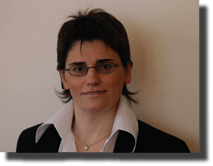
\includegraphics[width=0.25\textwidth]{../figures/samarati}}
    \subfigure[Sweeney]{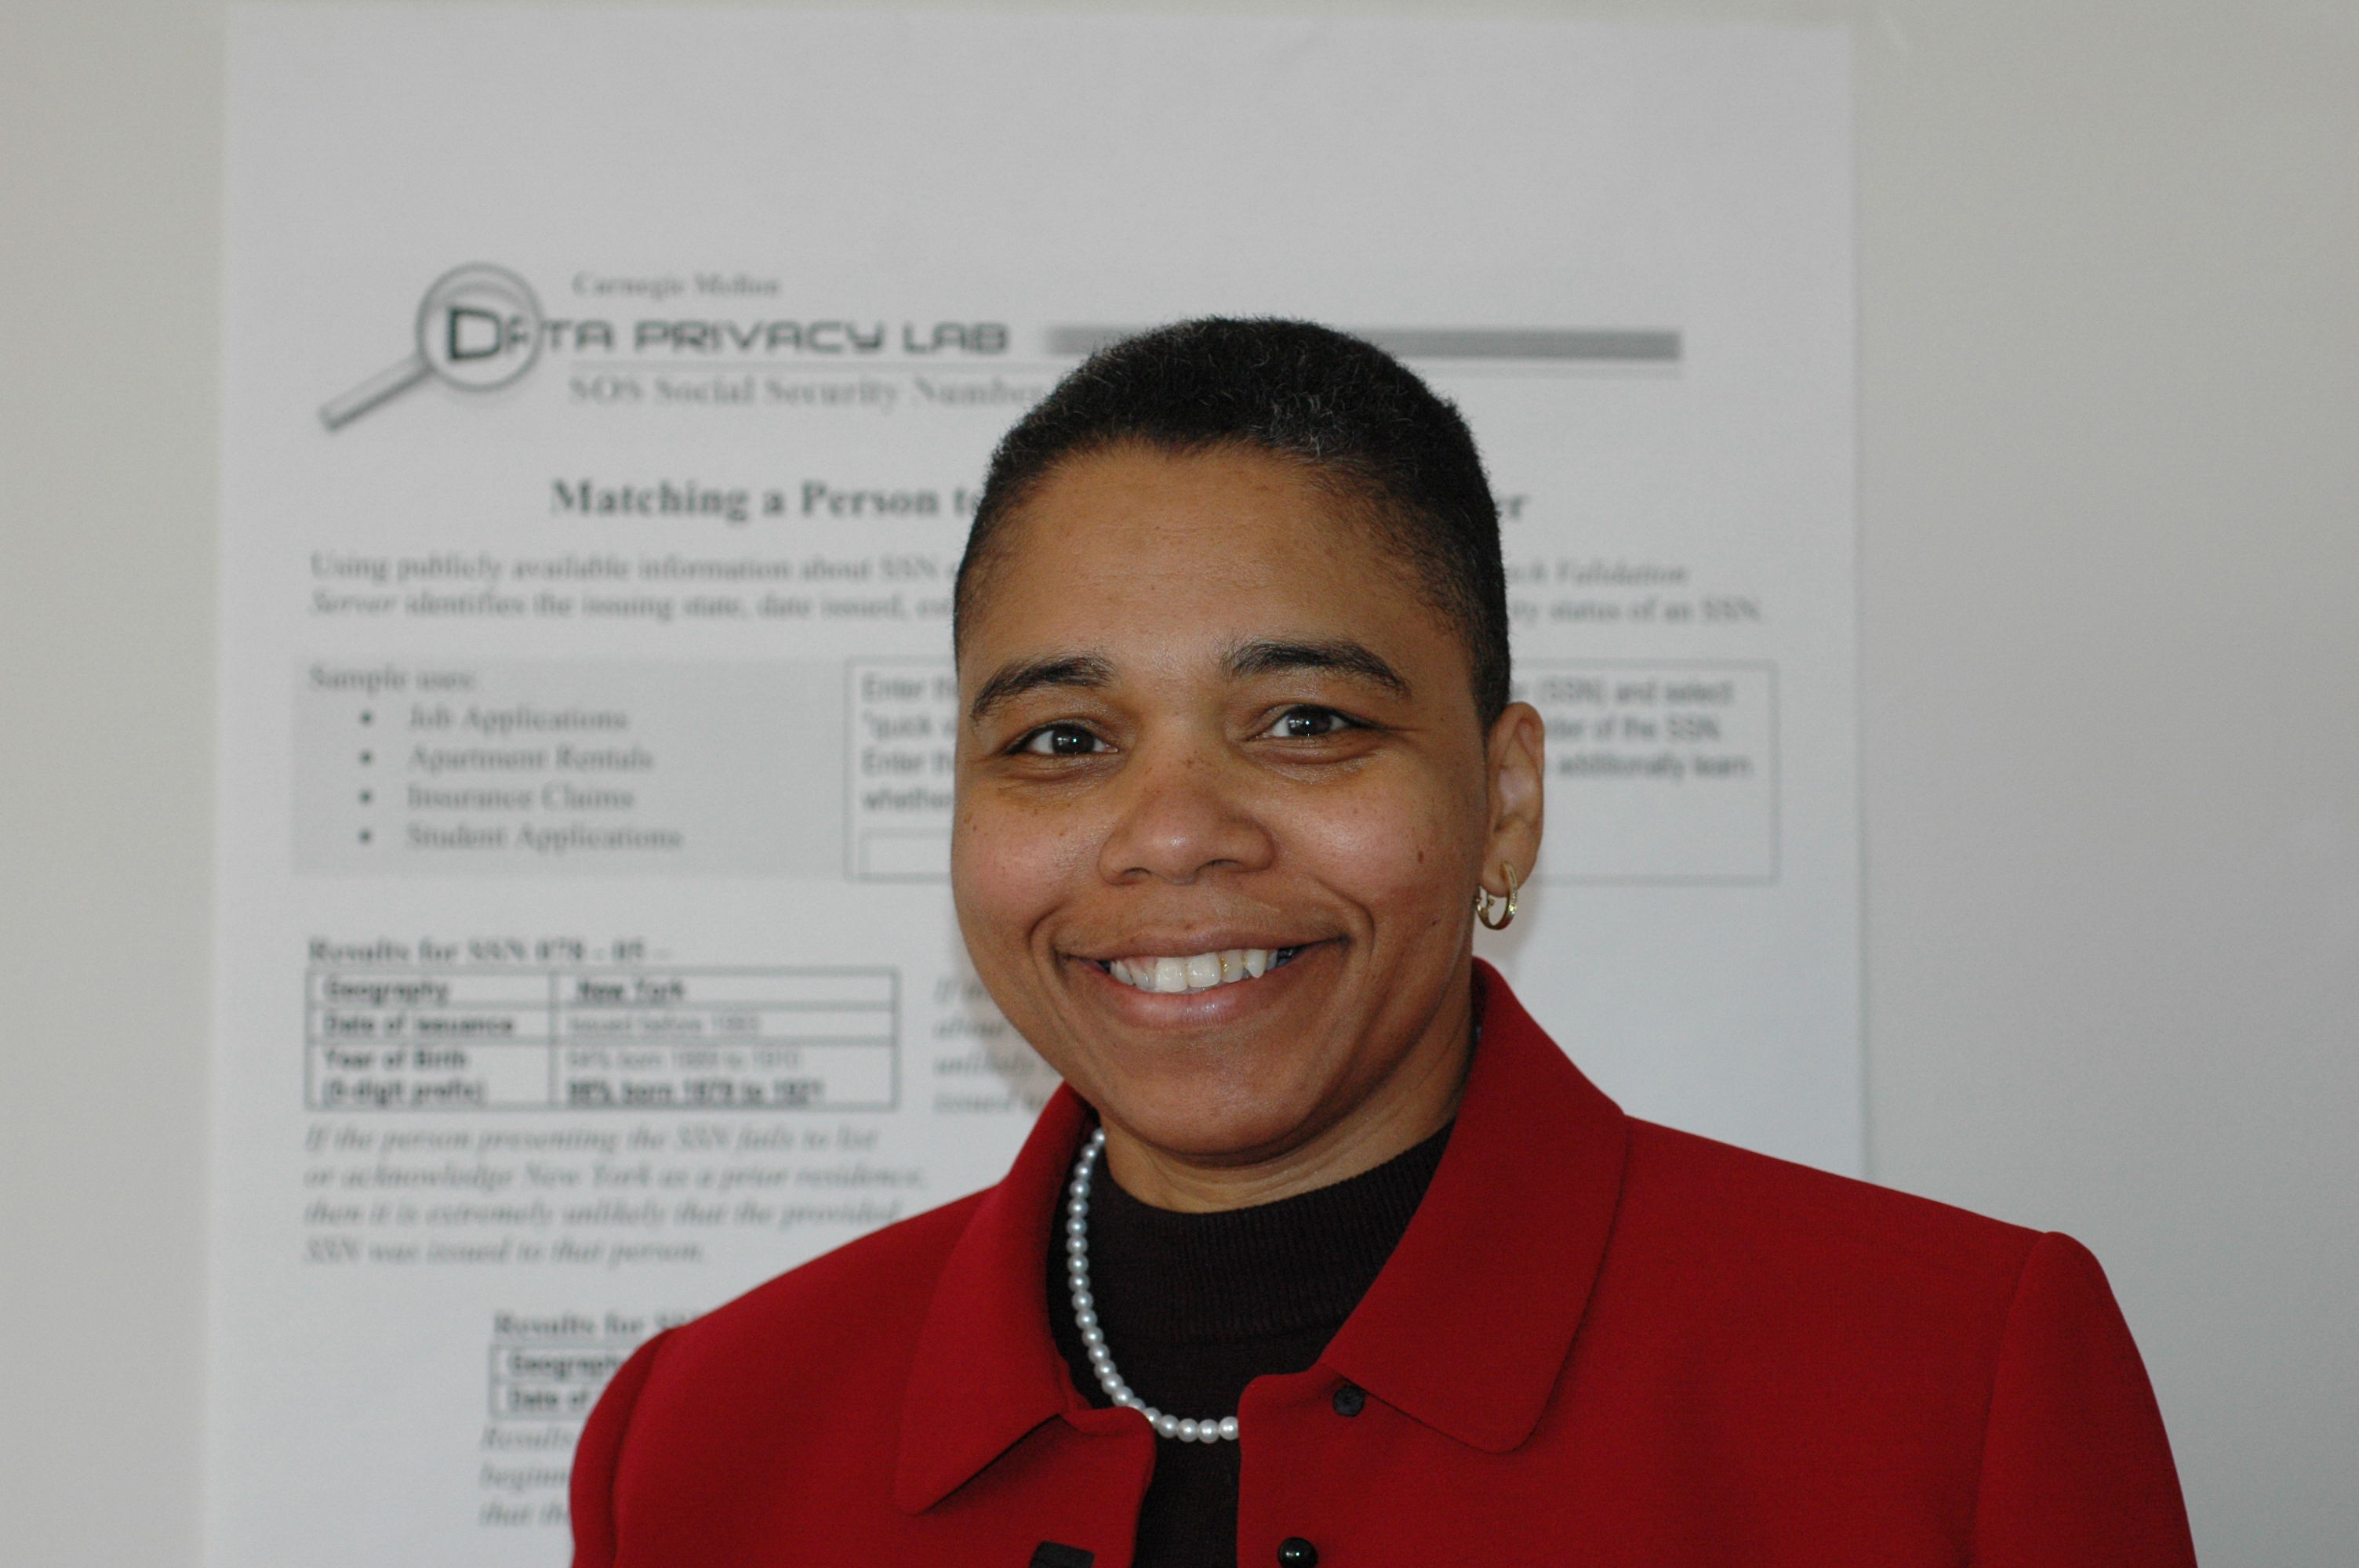
\includegraphics[width=0.25\textwidth]{../figures/sweeney}}
  \end{figure}
  \only<article>{The concept of $k$-anonymity was introduced by~\citet{samarati1998protecting} and provides good guarantees when accessing a single database}

  \begin{definition}[$k$-anonymity]
    A database provides $k$-anonymity if for every person in the database is indistinguishable from $k-1$ persons with respect to \emph{quasi-identifiers}.
  \end{definition}
  \alert{It's the analyst's job to define quasi-identifiers}
  
\end{frame}

\begin{frame}
  \only<1>{
    \begin{table}[H]
      \begin{tabular}{l|l|l|l|l|l|l}
        Birthday & Name & Height  & Weight & Age & Postcode & Profession\\
        \hline
        06/07 & Li Pu & 190 & 80 & 60+ & 1001 & Politician\\
        06/14 & Sara Lee & 185 & 110 & 60+ & 1001 & Rentier\\
        06/12 & Nikos Papadopoulos & 170 & 60 & 60+ & 1243 & Politician\\
        01/01 & A. B. Student & 170 & 70 & 40-60 & 6732 & Time Traveller\\
        05/08 & Li Yang & 175 & 72 & 30-40 & 6910 & Time Traveller
      \end{tabular}
      \caption{1-anonymity.}
    \end{table}

  }
  \only<presentation>{
    \only<2>{
      \begin{tabular}{l|l|l|l|l|l|l}
        Birthday & Name & Height  & Weight & Age & Postcode & Profession\\
        \hline
        06/07 &  & 190 & 80 & 60+ & 1001 & Politician\\
        06/14 &  & 185 & 110 & 60+ & 1001 & Rentier\\
        06/12 &  & 170 & 60 & 60+ & 1243 & Politician\\
        01/01 &  & 170 & 70 & 40-60 & 6732 & Time Traveller\\
        05/08 &  & 175 & 72 & 30-40 & 6910 & Policeman
      \end{tabular}
      1-anonymity
    }

    \only<3>{
      \begin{tabular}{l|l|l|l|l|l|l}
        Birthday & Name & Height  & Weight & Age & Postcode & Profession\\
        \hline
        06/07 &  & 180-190 & 80+ & 60+ & 1* & \\
        06/14 &  & 180-190 & 80+ & 60+ & 1* &\\
        06/12 &  & 170-180 & 60-80 & 60+ & 1* & \\
        01/01 &  & 170-180 & 60-80 & 20-60 & 6* &\\
        05/08 &  & 170-180 & 60-80 & 20-60 & 6* & 
      \end{tabular}
      1-anonymity
    }
  }
  \only<4>{
    \begin{table}[H]
      \begin{tabular}{l|l|l|l|l|l|l}
        Birthday & Name & Height  & Weight & Age & Postcode & Profession\\
        \hline
                 &  & 180-190 & 80+ & 60+ & 1* & \\
                 &  & 180-190 & 80+ & 60+ & 1* &\\
                 &  & 170-180 & 60-80 & 60+ & 1* & \\
                 &  & 170-180 & 60-80 & 20-60 & 6* &\\
                 &  & 170-180 & 60-80 & 20-60 & 6* & 
      \end{tabular}
      \caption{2-anonymity: the database can be partitioned in sets of at least 2 records}
    \end{table}
  }

  \only<article>{However, with enough information, somebody may still be able to infer something about the indivduals}
\end{frame}





\section{Differential privacy}
\only<article>{While $k$-anonymity can protect against specific re-identification attacks when used with care, it says little about what to do when the adversary has a lot of power. For example, if the  adversary knows the data of everybody that has participated in the database,  it is trivial for them to infer what our own data is. Differential privacy offers protection against adversaries with unlimited side-information or computational power. Informally, an algorithmic computation is differentially-private if an adversary cannot distinguish two similar database based on the result of the computation. While the notion of similarity is for the analyst to defined, a common is to say that two databases are similar when they are identical apart from the data of one person.}

\begin{frame}
  \begin{figure}[H]
    \begin{tikzpicture}
      \node[label=left:$x$] at (0,0) (data) {
\includegraphics[width=0.2\columnwidth]{../figures/medical}};

      \node[label=$x_1$] at (-2,3)(patient1) {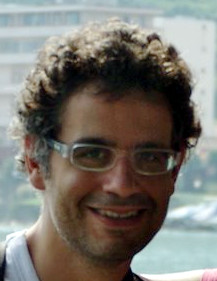
\includegraphics[width=0.1\columnwidth]{../figures/me-recent}};
      \uncover<3->{
        \node[label=$x_2$] at (2,3) (patient2) {
\includegraphics[width=0.2\columnwidth]{../figures/judge}};
      }
      \uncover<4->{
        \node[label=$a$] at (4,0)   (statistics) {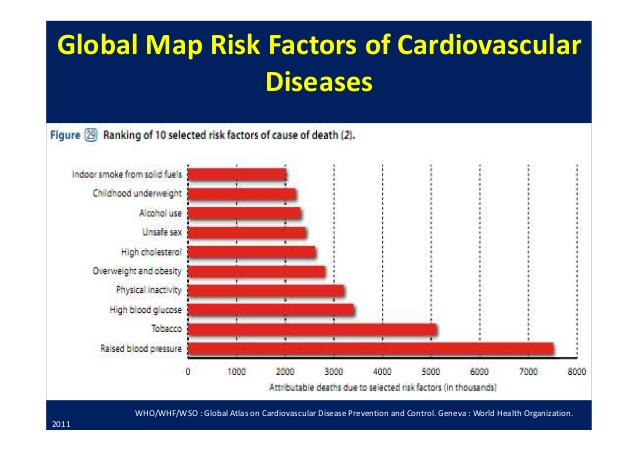
\includegraphics[width=0.3\columnwidth]{../figures/coronary-disease}};
      }
      \uncover<2->{
        \draw[->] (patient1) -- (data);
      }
      \uncover<3->{
        \draw[->] (patient2) -- (data);
      }
      \uncover<4->{
        \draw[->] (data) -- node[above]{$\pol$} (statistics);
      }
      \uncover<5->{
        \draw[line width=5, red, ->] (statistics) -- (patient2);
      }
    \end{tikzpicture}
    \caption{If two people contribute their data $x = (x_1, x_2)$ to a medical database, and an algorithm $\pol$ computes some public output $a$ from $x$, then it should be hard infer anything about the data from the public output.}
  \end{figure}

\end{frame}

\begin{frame}
  \frametitle{Privacy desiderata}
  \only<article>{
    Consider a scenario where $n$ persons give their data $x_1, \ldots, x_n$ to an analyst. This analyst then performs some calculation $f(x)$ on the data and published the result. The following properties are desirable from a general standpoint.

    \paragraph{Anonymity.} Individual participation in the study remains a secret. From the release of the calculations results, nobody can significantly increase their probability of identifying an individual in the database.

    \paragraph{Secrecy.} The data of individuals is not revealed. The release does not significantly increase the probability of inferring individual's information $x_i$.

    \paragraph{Side-information.} Even if an adversary has arbitrary side-information, he cannot use that to amplify the amount of knowledge he would have obtained from the release.

    \paragraph{Utility.} The released result has, with high probability, only a small error relative to a calculation that does not attempt to safeguard privacy.
  }
  \only<presentation>{
    We wish to calculate something on some private data and publish a \alert{privacy-preserving}, but \alert{useful}, version of the result.
    \begin{itemize}
    \item Anonymity: Individual participation remains hidden.
    \item Secrecy: Individual data $x_i$ is not revealed.
    \item Side-information: Linkage attacks are not possible.
    \item Utility: The calculation remains useful.
    \end{itemize}
  }
\end{frame}

\begin{frame}
  \frametitle{Example: The prevalence of drug use in sport}
  
  \only<article>{
    Let's say you need to perform a statistical analysis of the drug-use habits of athletes. Obviously, even if you promise the athlete not to reveal their information, you still might not convince them. Yet, you'd like them to be truthful. The trick is to allow them to randomly change their answers, so that you can't be \emph{sure} if they take drugs, no matter what they answer.
  }

  \only<presentation>{
    \begin{itemize}
    \item $n$ athletes
    \item Ask whether they have doped in the past year.
    \item Aim: calculate \% of doping.
    \item How can we get truthful / accurate results?
    \end{itemize}
  }
  \only<2>{
    \begin{block}{Algorithm for randomising responses about drug use}
      \begin{enumerate}
      \item Flip a coin.
      \item If it comes heads, respond truthfully. 
      \item Otherwise, flip another coin and respond \texttt{yes} if it comes heads and \texttt{no} otherwise.
      \end{enumerate}
    \end{block}

    If the rate of positive responses is $p$, everybody follows the protocol, and the coin is fair, what is the true rate $q$ of drug use?
  }
  \only<presentation>{
    \uncover<3>{
      \[
        p = 1/2 + q/2 \Rightarrow q = 1/2
      \]
    }
  }
  \only<article>{The problem with this approach, of course, is that we are effectively throwing away half of our data. In particular, if we repeated the experiment with a coin that came heads at a rate $\epsilon$, then our error bounds would scale as $O(1/\sqrt{\epsilon n})$ for $n$ data points.}
\end{frame}

\begin{frame}
  \frametitle{The randomised response mechanism}
  \only<article>{The above idea can be generalised. Consider we have data $x_1, \ldots, x_n$ from $n$ users and we transform it randomly to $y_1, \ldots, y_n$ using the following mapping.}
  \begin{definition}[Randomised response]
    The $i$-th user, whose data is $x_i \in \{0,1\}$ , responds with $a_i \in \{0, 1\}$ with probability
    \[
      \pol(a_i = j \mid x_i = k) = p,  \qquad  \pol(a_i = k \mid x_i = k) = 1 - p,
    \]
    where $j \neq k$.
  \end{definition}

  \uncover<2->{Given the complete data $x$, the mechanism's output is $a = (a_1, \ldots, a_n)$.}
  \uncover<3->{Since the algorithm independently calculates a new value for each data entry, the output is
    \[
      \pol(a \mid x) = \prod_i \pol(a_i \mid x_i)
    \]
  }

  \only<article>{This mechanism satisfies so-called $\epsilon$-differential privacy, which we will define later.}

\end{frame}

\begin{frame}
  \begin{exercise}
    Let the adversary have a prior $\bel(x = 0) = 1 - \bel(x = 1)$ over the values of the true response of an individual. we use the randomised response mechanism with $p$ and the adversary observes the randomised data $a = 1$ for that individual, then what is $\bel(x = 1 \mid a = 1)$?
  \end{exercise}
\end{frame}

\begin{frame}
  \frametitle{The local privacy model}
  \begin{figure}[H]
    \centering
    \begin{tikzpicture}
      \node[RV] at (0,0) (x1) {$x_1$};
      \node[RV] at (0,1) (x2) {$x_2$};
      \node[RV] at (0,2) (xn) {$x_n$};
      \node[RV] at (2,0) (a1) {$a_1$};
      \node[RV] at (2,1) (a2) {$a_2$};
      \node[RV] at (2,2) (an) {$a_n$};
      \draw[->] (x1) -- (a1);
      \draw[->] (x2) -- (a2);
      \draw[->] (xn) -- (an);
      % \node[select] at (1,-1) (pol) {$\pol$};
      % \draw[->] (pol) -- (a1);
      % \draw[->] (pol) -- (a2);
      % \draw[->] (pol) -- (an);
    \end{tikzpicture}
    
    \caption{The local privacy model}
    \label{fig:local-privacy}
  \end{figure}
\end{frame}

\begin{frame}
  \frametitle{Differential privacy.}
  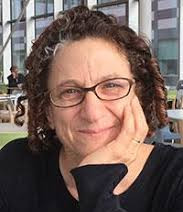
\includegraphics[width=0.2\textwidth]{../figures/dwork} \hspace{1em}
  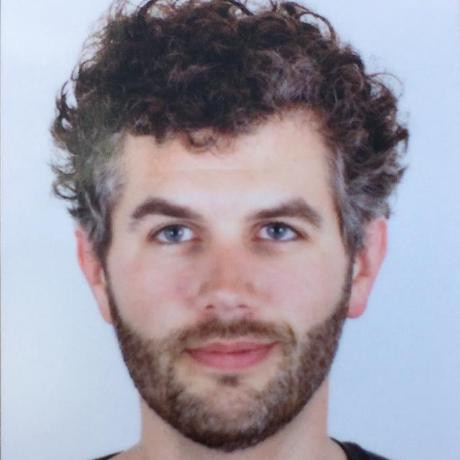
\includegraphics[width=0.2\textwidth]{../figures/mcsherry} \hspace{1em}
  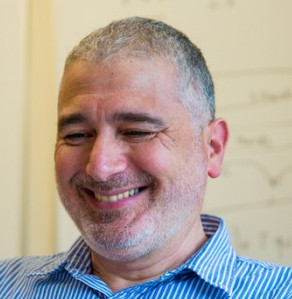
\includegraphics[width=0.2\textwidth]{../figures/nissim} \hspace{1em}
  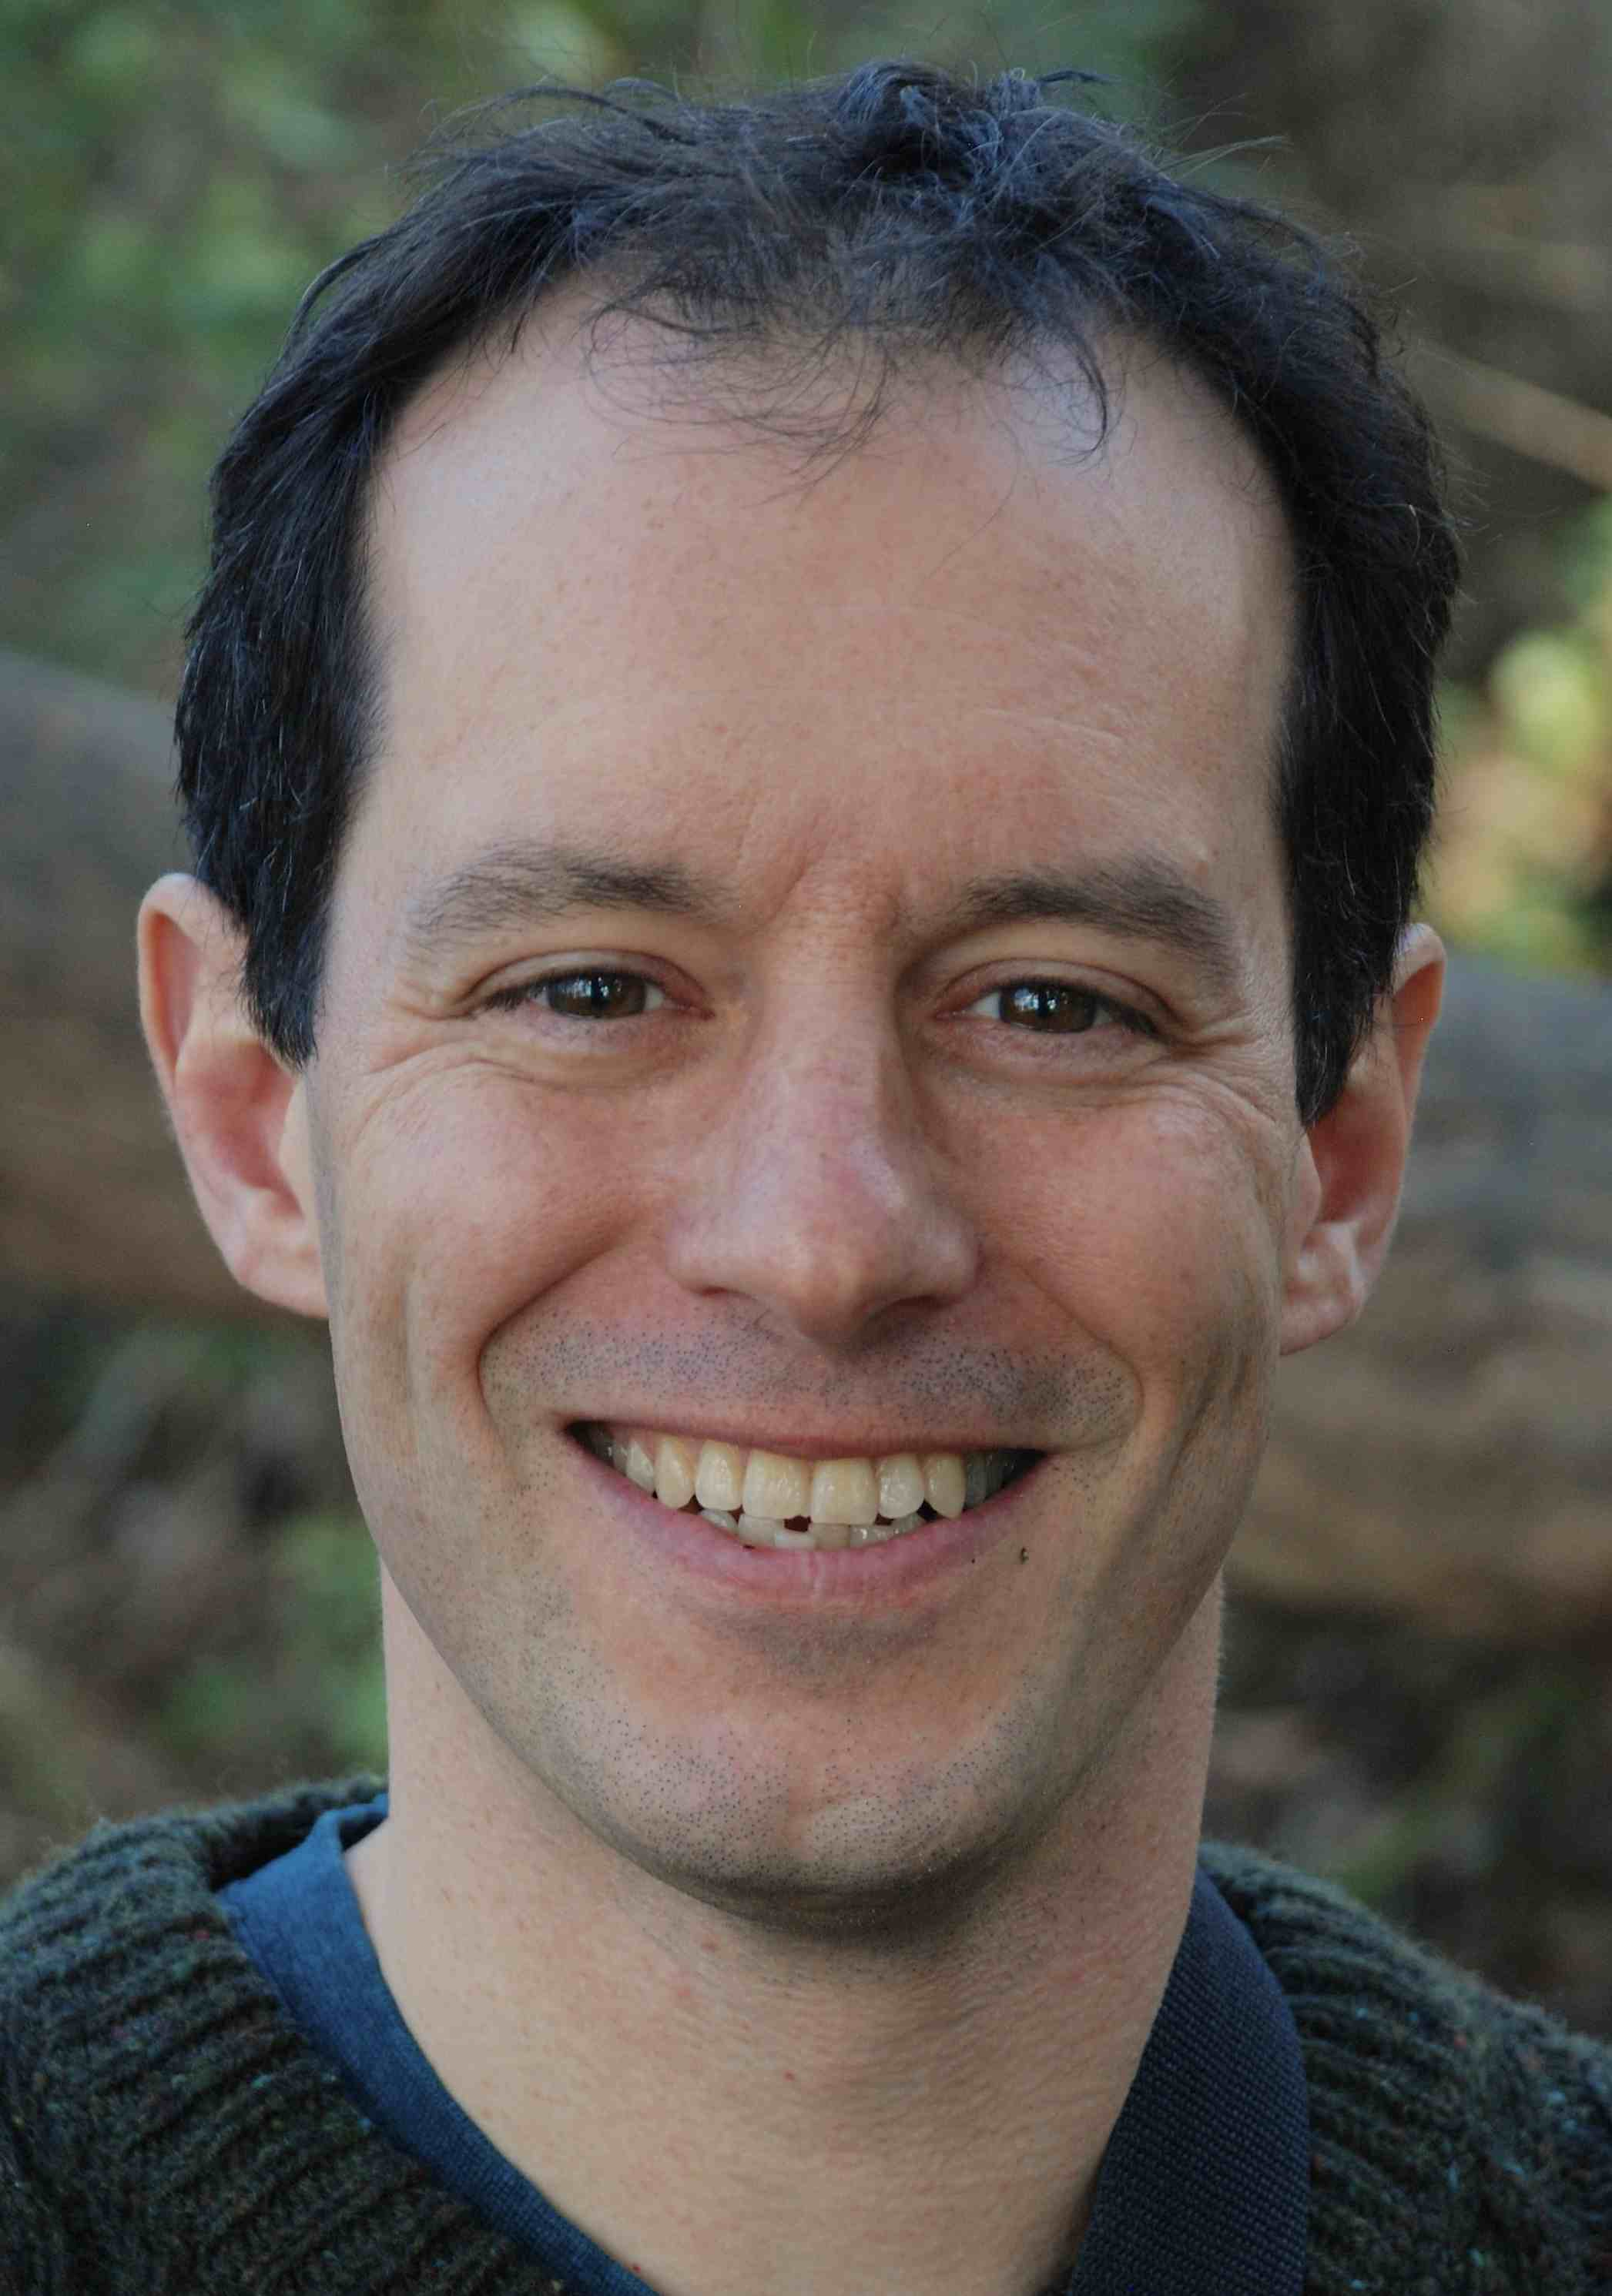
\includegraphics[width=0.2\textwidth]{../figures/smith}
  \only<article>{Now let us take a look at a way to characterise the  the inherent privacy properties of algorithms. This is called differential privacy, and it can be seen as a bound on the information an adversary with arbitrary power or side-information could extract from a computation.}
  
  \begin{definition}[$\epsilon$-Differential Privacy]
    A stochastic algorithm $\pol : \CX \to \CA$, where $\CX$ is endowed with a neighbourhood relation $N$, is said to be $\epsilon$-differentially private if
    \begin{equation}
      \label{eq:epsilon-dp}
      \left|\ln \frac{\pol(a \mid x)}{\pol(a \mid x')}\right| \leq \epsilon , \qquad \forall x N x'.
    \end{equation}
  \end{definition}
  
  \only<article>{Typically, algorithms are applied to datasets $x = (x_1, \ldots, x_n)$ composed of the data of $n$ individuals. Thus, all privacy guarantees relate to the data contributed by these individuals. 

    In this context, two datasets are usually called neighbouring if $x = (x_1, \ldots, x_{i-1}, x_i, x_{i+1} x_n)$ and 
    $x' = (x_1, \ldots, x_{i-1}, x_{i+1} x_n)$, i.e. if one dataset is missing an element.
    
    A slightly weaker definition of neighbourhood is to say that $x N x'$ if $x' = (x_1, \ldots, x_{i-1}, x'_i, x_{i+1} x_n)$, i.e. if one dataset has an altered element.

  }
\end{frame}

\begin{frame}
  \only<article>{
    \begin{remark}
      Any differentially private algorithm must be stochastic.
    \end{remark}

    To prove that this is necessary, consider the example of counting how many people take drugs in a competition. If the adversary only doesn't know whether you in particular take drugs, but knows whether everybody else takes drugs, it's trivial to discover your own drug habits by looking at the total. This is because in this case, $f(x) = \sum_i x_i$ and the adversary knows $x_i$ for all $i \neq j$. Then, by observing $f(x)$, he can recover $x_j = f(x) - \sum_{i \neq j} x_i$. Consequently, it is not possible to protect against adversaries with arbitrary side information without stochasticity.}
  \begin{remark}
    The randomised response mechanism with $p \leq 1/2$ is $(\ln \frac{1 - p}{p})$-DP.
  \end{remark}
  \begin{proof}
    Consider $x = (x_1, \ldots, x_i,  \ldots, x_n)$, $x' = (x_1, \ldots, x'_i,  \ldots, x_n)$. Then
    \begin{align*}
      \pol(a \mid x)
      \uncover<2->{&= \prod_i \pol(a_i \mid x_i)}
                     \uncover<3->{\\ &= \pol(a_j \mid x_j') \prod_{i \neq j} \pol(a_i \mid x_i) }
                                       \uncover<4->{\\ &\leq \frac{p}{1 - p} \pol(a_j \mid x_j) \prod_{i \neq j} \pol(a_i \mid x_i) }
                                                         \uncover<5>{\\ &= \frac{1-p}{p} \pol(a \mid x')}
    \end{align*}
    \only<4>{$\pol(a_j = k\mid x_j = k) = 1 - p$ so the ratio is $\max\{(1-p)/p, p/(1 - p)\} \leq (1 - p)/p$ for $p \leq 1/2$.}
  \end{proof}
\end{frame}

\begin{frame}
  \begin{figure}[H]
    \centering
    \begin{tikzpicture}
      \node[rectangle] at (0,0) (python) {Python program};
      \node[rectangle] at (8,0) (database) {Database System};
      \draw[thickarrow, bend right]   (python) to node[black]{Query $q$} (database) ;
      \draw[thickarrow, bend right]   (database) to node[black]{Private response $a$} (python) ;
    \end{tikzpicture}
    \label{fig:database-access}
    \caption{Private database access model}
  \end{figure}
  \begin{block}{Response policy}
    The  policy defines a distribution over responses $a$ given the data $x$ and the query $q$.
    \[
      \pol(a \mid x, q)
    \]
  \end{block}
\end{frame}

\begin{frame}
  \frametitle{Differentially private queries}
  \begin{block}{The \texttt{DP-SELECT} statement}
    \begin{itemize}
    \item \texttt{DP-SELECT column1, column2 FROM table;}
      \only<article>{This selects only some columns from the table}
    \item \texttt{DP-SELECT * FROM table;}
      \only<article>{This selects all the columns from the table}
    \end{itemize}
  \end{block}

  \begin{block}{Selecting rows}
    \texttt{SELECT * FROM table WHERE column = value;}
  \end{block}

  \begin{exampleblock}{Arithmetic queries}
    \only<article>{Here are some example SQL statements}
    \begin{itemize}
    \item  \texttt{DP-SELECT COUNT(column) FROM table WHERE condition;}
      \only<article>{This allows you to count the number of rows matching \texttt{condition}}
    \item  \texttt{DP-SELECT AVG(column) FROM table WHERE condition;}
      \only<article>{This lets you to count the number of rows matching \texttt{condition}}
    \item  \texttt{DP-SELECT SUM(column) FROM table WHERE condition;}
      \only<article>{This is used to sum up the values in a column.}
    \end{itemize}
  \end{exampleblock}

  \begin{alertblock}{Cumulative privacy loss}
    Depending on the DP scheme, each query answered may leak privacy.
    \only<article>{In particular, if we always respond with an $\epsilon$-DP mechanism, after $T$ queries our privacy guarantee is $T \epsilon$. There exist mechanisms that do not respond to each query independently, which can bound the total privacy loss.}
  \end{alertblock}
\end{frame}

\begin{frame}
  \begin{exercise}{Adversary knowledge}
    \only<article>{Assume that the adversary knows that the data is either $\bx$ or $\bx'$. For concreteness, assume the data is either }
    \[
      \bx = (x_1, \ldots, x_j = 0, \ldots,  x_n)
    \]
    \only<article>{where $x_i$ indicates whether or not the $i$-th person takes drugs, or}
    \[
      \bx' = (x_1, \ldots, x_j=1, \ldots, x_n).
    \]
    \only<article>{In other words, the adversary knows the data of all people apart from one, the $j$-th person. We can assume that the adversary has some prior belief}
    \[
      \bel(\bx) = 1 - \bel(\bx')
    \]
    \only<article>{for the two cases. Assume the adversary knows
      the output $a$ of a mechanism $\pol$}
    \only<presentation>{
      \onslide<2->{
        \[
          a_t, \qquad \pol(a_t \mid \bx_t) \Rightarrow
          \begin{cases}
            \pol(a_t \mid \bx_t = \bx)\\
            \pol(a_t \mid \bx_t = \bx')
          \end{cases}
        \]
      }
    }
    What can we say about the posterior distribution of the adversary $\bel(\bx \mid a, \pol)$ after having seen the output, if $\pol$ is $\epsilon$-DP?
  \end{exercise}
  
\end{frame}
\only<article>{
  \begin{frame}
    \begin{block}{Solution}
      We can write the adversary posterior as follows.
      \begin{align}
        \bel(\bx \mid a, \pol)
        &=
        \frac{\pol(a  \mid \bx) \bel(\bx)}
          {\pol(a  \mid \bx) \bel(\bx) + \pol(a  \mid \bx') \bel(\bx')}
        \\
        &\geq
          \frac{\pol(a  \mid \bx) \bel(\bx)}
          {\pol(a  \mid \bx) \bel(\bx) + \pol(a  \mid \bx) e^\epsilon \bel(\bx')} \tag{from DP definition}
        \\
        &=
          \frac{\bel(\bx)}
          {\bel(\bx) +  e^\epsilon \bel(\bx')}
      \end{align}
      But this is not very informative. We can also write
      \begin{align}
        \frac{\bel(\bx \mid a, \pol)}{\bel(\bx' \mid a, \pol)}
        =
        \frac{\pol(a  \mid \bx) \bel(\bx)}{\pol(a  \mid \bx') \bel(\bx')}
        \geq
        \frac{\pol(a  \mid \bx) \bel(\bx)}{\pol(a  \mid \bx) e^{-\epsilon} \bel(\bx')}
        =
        \frac{\bel(\bx)}{\bel(\bx')} e^\epsilon
      \end{align}
    \end{block}
  \end{frame}
}
\subsection{Other differentially private mechanisms}
\begin{frame}
  \frametitle{The Laplace mechanism.}
  \only<article>{
    A simple method to obtain a differentially private algorithm from a deterministic function $f : \CX \to \Reals$, is to use additive noise, so that the output of the algorithm is simply 
    \[
      a = f(x) + \omega, \qquad \omega \sim \Laplace.
    \]
    The amount of noise added, together with the smoothness of the function $f$, determine the amount of privacy we have.
  }
  \begin{definition}[The Laplace mechanism]
    For any function $f : \CX \to \Reals$, 
    \begin{equation}
      \label{eq:laplace-mechanism}
      \pol(a \mid x) = \Laplace(f(x), \lambda),
    \end{equation}
    where the Laplace density is defined as
    \[
      p(\omega \mid \mu, \lambda) = \frac{1}{2 \lambda} \exp\left(-\frac{|\omega - \mu|}{\lambda}\right).
    \]
  \end{definition}
  \only<article>{Here, $\Laplace(\mu, \lambda)$ is the density $f(x) = \frac{\lambda}{2} \exp(-\lambda |x - \mu|)$}.
\end{frame}

\begin{frame}
  \begin{example}[Calculating the average salary]
    \begin{itemize}
    \item The $i$-th person receives salary $x_i$
    \item We wish to calculate the average salary in a private manner.
    \end{itemize}
  \end{example}
  \begin{block}{Local privacy model}
    \begin{itemize}
    \item Obtain $y_i = x_i + \omega$, where $\omega \sim \Laplace(\lambda)$.
    \item Return $a = n^{-1} \sum_{i=1}^n y_i$.
    \end{itemize}
  \end{block}
  \begin{block}{Centralised privacy model}
    Return $a = n^{-1} \sum_{i=1}^n x_i + \omega$, where $\omega \sim \Laplace(\lambda')$.
  \end{block}
  
  How should we add noise in order to guarantee privacy?
\end{frame}

\begin{frame}
  \frametitle{The local privacy model}
  \begin{figure}[H]
    \centering
    \begin{tikzpicture}
      \node[RV] at (0,0) (x1) {$x_1$};
      \node[RV] at (0,1) (x2) {$x_2$};
      \node[RV] at (0,2) (xn) {$x_n$};
      \node[RV] at (2,1) (a) {$a$};
      \node[select] at (1,-1) (pol) {$\pol$};
      \draw[->] (x1) -- (a);
      \draw[->] (x2) -- (a);
      \draw[->] (xn) -- (a);
      \draw[->] (pol) -- (a);
    \end{tikzpicture}
    
    \caption{The centralised privacy model}
    \label{fig:centralised-privacy}
  \end{figure}
\end{frame}

\begin{frame}
  \frametitle{DP properties of the Laplace mechanism}
  \begin{definition}[Sensitivity]
    The sensitivity of a function $f$ is
    \[
      \sensitivity{f} \defn \sup_{x N x'} |f(x) - f(x')|
    \]
    \only<article>{
      If we define a metric $d$, so that $d(x, x') = 1$ for $x N x'$, then:
      \[
        |f(x) - f(x')| \leq \sensitivity{f} d(x, x'),
      \]
      i.e. $f$ is $\sensitivity{f}$-Lipschitz with respect to $d$.
    }
  \end{definition}
  \begin{theorem}
    The Laplace mechanism on a function $f$ ran with $\Laplace(\lambda)$ is $\sensitivity{f} / \lambda$-DP.
  \end{theorem}
  \begin{proof}
    \begin{align*}
      \frac{\pol(a \mid x)}{\pol(a \mid x')}
      &=
        \frac{e^{|a - f(x')|/\lambda}}{e^{|a - f(x)|/\lambda}}
        \leq
        \frac{e^{|a - f(x)|/\lambda + \sensitivity{f}/\lambda}}{e^{|a - f(x)|/\lambda}}
        = e^{\sensitivity{f} / \lambda}
    \end{align*}
  \end{proof}
  
  What is the effect of applying the Laplace mechanism in the local versus centralised model?
  \only<article>{
    Here let us assume $x_i \in [0, M]$ for all $i$.
    \begin{block}{Laplace in the local privacy model}
      The sensitivity of the individual data is $M$, so to obtain $\epsilon$-DP we need to use $\lambda = M / \epsilon$. The variance of each component is $2M/\epsilon$, so the total variance is $2M/\epsilon n$.
    \end{block}
    \begin{block}{Laplace in the centralised privacy model}
      The sensitivity of $f$ is $M / n$, so we need to use $\lambda = M / n\epsilon$. The variance of $a$ is $M / \epsilon n$.
    \end{block}
  }
\end{frame}

\subsection{Utility of queries}

\begin{frame}
  \only<article>{Rather than saying that we wish to calculate a private version of some specific function $f$, sometimes it is more useful to consider the problem from the perspective of the utility of different answers to queries. More precisely, imagine the interaction between a database system and a user:}
  \begin{block}{Interactive queries}
    \begin{itemize}
    \item System has data $x$.
    \item User asks query $q$.
    \item System responds with $a$.
    \item There is a common utility function
      $\util : \CX, \CA, \CQ \to \Reals$.
    \end{itemize}
  \end{block}
  \only<article>{The utility $U(x,a,q)$  describes how appropriate each response $a$ given by the system for a query $r$ is given the data $x$. It can be seen as how useful the response is to the user, and allows us to quantify exactly how much we }

\end{frame}
\begin{frame}
  \frametitle{The Exponential Mechanism.}
  \only<article>{
    Here we assume that we can answer queries $q$, whereby each possible answer $a$ to the query has a different utility to the DM: $\util(q, a, x)$.
    Let $\sensitivity{\util(q)} \defn \sup_{x N x'} |\util(q, a, x) -\util(q, a, x)|$ denote the sensitivity of a query. Then the following mechanism is $\epsilon$-differentially private.
  }
  \begin{definition}[The Exponential mechanism]
    For any utility function $\util : \CQ \times \CA \times \CX \to \Reals$, define the policy
    \begin{equation}
      \label{eq:exponential-mechanism}
      \pol(a \mid x) \defn \frac{e^{\epsilon \util(q, a, x) / \sensitivity{ \util(q)}}}{\sum_{a'} e^{\epsilon \util(q, a', x) / \sensitivity{\util(q)}}}
    \end{equation}
  \end{definition}
  \only<presentation>{
    What happens when $\epsilon \to \infty$? What about when $\epsilon \to 0$?
  }
  \only<article>{
    Clearly, when $\epsilon \to 0$, this mechanism is uniformly random. When $\epsilon \to \infty$ the action maximising $\util(q,a,x)$ is always chosen.
  }
\end{frame}


\subsection{Privacy and reproducibility}

\begin{frame}
  \frametitle{The unfortunate practice of adaptive analysis}
  \begin{tikzpicture}
    \node<1->[rectangle] at (0,4) (prior) {Prior};
    \node<2->[rectangle] at (0,0) (training) {Training data};
    \node<3->[rectangle] at (4,4) (posterior) {Posterior};
    \node<5->[rectangle] at (8,4) (posterior2) {Posterior'};
    \node<2->[rectangle] at (4,0) (holdout) {Holdout};
    \node<4->[RV] at (4,2) (result) {Result};
    \node<5->[RV] at (8,2) (result2) {Result'};
    \draw<3->[medarrow] (training)--(posterior);
    \draw<3->[medarrow] (prior)--(posterior);
    \draw<4->[medarrow] (posterior)--(result);
    \draw<4->[medarrow] (holdout)--(result);
    \draw<5->[red,medarrow] (posterior2)--(result2);
    \draw<5->[red,medarrow] (holdout)--(result2);
    \draw<5->[red,medarrow] (result)--(posterior2);
    \draw<5->[red,medarrow] (posterior)--(posterior2);
  \end{tikzpicture}
  \only<article>{In the ideal data analysis, we start from some prior hypothesis, then obtain some data, which we split into training and holdout. We then examine the training data and obtain a posterior that corresponds to our conclusions. We can then measure the quality of these conclusions in the independent holdout set.

    However, this is not what happens in general. Analysts typically use the same holdout repeatedly, in order to improve the performance of their algorithms. This can be seen as indirectly using the holdout data to obtain a new posterior, and so it is possible that you can overfit on the holdout data, even if you never directly see it. It turns out we can solve this problem if we use differential privacy, so that the analyst only sees a differentially private version of queries.
  }
\end{frame}


\begin{frame}
  \frametitle{The reusable holdout~\cite{dwork2015reusable}\footnote{Also see \url{https://ai.googleblog.com/2015/08/the-reusable-holdout-preserving.html}}}
  \only<article>{One idea to solve this problem is to only allow the analyst to see a private version of the result. In particular, the analyst will only see whether or not the holdout result is $\tau$-close to the training result.}

  \begin{block}{Algorithm parameters}
    \begin{itemize}
    \item Performance measure $f$.
    \item Threshold $\tau$. \only<article>{How close do we want $f$ to be on the training versus holdout set?}
    \item Noise $\sigma$. \only<article>{How much noise should we add?}
    \item Budget $B$. \only<article>{How much are we allowed to learn about the holdout set?}

    \end{itemize}
  \end{block}
\end{frame}

\begin{frame}
  \frametitle{Learning outcomes}
  \begin{block}{Understanding}
    \begin{itemize}
    \item Linkage attacks and $k$-anonymity.
    \item Inferring data from summary statistics.
    \item The local versus global differential privacy model.
    \item False discovery rates.
    \end{itemize}
  \end{block}
  
  \begin{block}{Skills}
    \begin{itemize}
    \item Make a dataset satisfy $k$-anonymity with respect to identifying attributes.
    \item Apply the randomised response and Laplace mechanism to data.
    \item Apply the exponential mechanism to simple decision problems.
    \item Use differential privacy to improve reproducibility.
    \end{itemize}
  \end{block}

  \begin{block}{Reflection}
    \begin{itemize}
    \item How can potentially identifying attributes be chosen to achieve $k$-anonymity?
    \item How should the parameters of the two ideas, $\epsilon$-DP and $k$-anonymity be chosen?
    \item Does having more data available make it easier to achieve privacy?
    \end{itemize}
  \end{block}
  
\end{frame}

  
%%% Local Variables:
%%% mode: latex
%%% TeX-engine: xetex
%%% TeX-master: "notes"
%%% End:

 %data bases

\chapter{Fairness}
\only<article>{
  When machine learning algorithms are applied at scale, it can be difficult to imagine what their effects might be. In this part of the course, we consider notions of fairness as seen through the prism of conditional independence and meritocracy. The first notion requires that we look deeper into directed graphical models.
}
\section{Graphical models}
\only<article>{
  Graphical models are a very useful tool for modelling the relationship between multiple variables. The simplest such models, probabilistic graphical models (otherwise known as Bayesian networks) involve directed acyclic graphs between random variables. There are two other types of probabilistic models, factor graph and undirected graphical models, which are equivalent to each other, though not to directed models.}
\begin{frame}
  \frametitle{Graphical models}
  \begin{figure}[H]
    \centering
    \begin{tikzpicture}
      \node[RV] at (2,0) (xi) {$x_3$};
      \node[RV] at (0,0) (xB) {$x_1$};
      \node[RV] at (1,1) (xD) {$x_2$};
      \draw[->] (xB) to (xD);
      \draw[->] (xD) to (xi);
      \draw[->] (xB) to (xi);
    \end{tikzpicture}
    \label{fig:bn}
    \caption{Graphical model (directed acyclic graph) for three variables.}
  \end{figure}
  \only<article>{Consider for example the model in Figure~\ref{fig:bn}. It involves three variables, $x_1, x_2, x_3$ and there are three arrows, which show how one variable depends on another. Simply put, if you think of each $x_k$ as a stochastic function, then $x_k$'s value only depends on the values of its parents, i.e. the nodes that are point to it. In this example, $x_1$ does not depend on any other variable, but the value of $x_2$ depends on the value of $x_1$. Such models are useful when we want to describe the joint probability distribution of all the variables in the collection.}
  \begin{block}{Joint probability}
    Let $\bx = (x_1, \ldots, x_n)$. Then $\bx : \Omega \to X$, $X = \prod_i X_i$ and:
    \[
    \Pr(\bx \in A) = P(\cset{\omega \in \Omega}{\bx(\omega) \in A}).
    \]
  \end{block}
  \only<article>{
    When $X_i$ are finite, we can typically write
    \[
    \Pr(\bx = \ba) = P(\cset{\omega \in \Omega}{\bx(\omega) = \ba}),
    \]
    for the probability that $x_i = a_i$ for all $i \in [n]$.
  }
  \begin{block}{Factorisation}
    \only<article>{
      For any subsets $B \subset [n]$ and its complement $C$ so that
      $\bx_B = (x_i)_{i \in B}$,     $\bx_C = (x_i)_{i \notin B}$
    }
    \only<1>{
      \[
      \Pr(\bx) = \Pr(\bx_B \mid \bx_C) \Pr(\bx_C)
      \only<presentation>{,\qquad B, C \subset [n]}
      \]
    }
    \uncover<2->{
      So we can write any joint distribution as
      \[
      \Pr(x_1) \Pr(x_2 \mid x_1) \Pr(x_3 \mid x_1, x_2) \cdots \Pr(x_n \mid x_1, \ldots, x_{n-1}).
      \]
    }
  \end{block}
  \only<article>{Although the above factorisation is always possible to do, sometimes our graphical model has a structure that makes the factors much simpler. In fact, the main reason for introducing graphical models is to represent dependencies between variables. For a given model, we can infer whether some variables are in fact dependent, independent, or conditionally independent.}
\end{frame}
\begin{frame}
  \frametitle{Directed graphical models and conditional independence}
  \begin{figure}[H]
    \centering
    \begin{tikzpicture}
      \node[RV] at (2,0) (xi) {$x_3$};
      \node[RV] at (0,0) (xB) {$x_1$};
      \node[RV] at (1,1) (xD) {$x_2$};
      \draw[->] (xB)--(xD);
      \draw[->] (xD)--(xi);
    \end{tikzpicture}
    \label{fig:bn}
    \caption{Graphical model for the factorisation $\Pr(x_3 \mid x_2) \Pr(x_2 \mid x_1) \Pr(x_1)$.}
  \end{figure}
  \begin{block}{Conditional independence}
    We say $x_i$ is conditionally independent of $\bx_B$ given $\bx_D$ and write $x_i \mid \bx_D \indep \bx_B$ iff
    \[
    \Pr(x_i, \bx_B \mid \bx_D)
    =
    \Pr(x_i \mid \bx_D)
    \Pr(\bx_B \mid \bx_D).
    \]
  \end{block}

  \frametitle{Directed graphical models}
  \only<article>{
    A graphical model is a convenient way to represent conditional independence between variables. There are many variants of graphical models, whose name is context dependent. Other names used in the literature are probabilistic graphical models, Bayesian networks, causal graphs, or decision diagrams. In this set of notes we focus on directed graphical models that depict dependencies between ranom variables.

    \begin{definition}[Directed graphical model] A collection of $n$ random variables $x_i : \Omega \to X_i$, and let $X \defn \prod_i X_i$, with underlying probability measure $P$ on $\Omega$.
      Let $\bx = (x_i)_{i=1}^n$ and for any subset $B \subset[n]$ let
      \begin{align}
        \bx_B &\defn (x_i)_{i \in B}\\
        \bx_{-j} &\defn (x_i)_{i \neq i}
      \end{align}
    \end{definition}
  }
  \only<article>{In a graphical model, conditional independence is represented through directed edges.}


\end{frame}

\begin{frame}
  \begin{example}[Smoking and lung cancer]
    \begin{figure}[H]
      \centering
      \begin{tikzpicture}
        \node[RV] at (0,0) (x1) {$S$};
        \node[RV] at (1,1) (x2) {$C$};
        \node[RV] at (2,0) (x3) {$A$};
        \draw[->] (x1)--(x2);
        \draw[->] (x3)--(x2);
      \end{tikzpicture}
      \caption{Smoking and lung cancer graphical model, where $S$: Smoking, $C$: cancer, $A$: asbestos exposure.}
    \end{figure}
    \only<article>{
      It has been found by~\citet{lee2001relation} that lung  incidence not only increases with both asbestos exposure and smoking. This is in agreement with the graphical model shown. The study actually found that there is an amplification effect, whereby smoking and asbestos exposure increases cancer risk by 28 times compared to non-smokers. This implies that the risk is not simply additive. The graphical model only tells us that there is a dependency, and does not describe the nature of this dependency precisely.}
  \end{example}
  \begin{block}{Explaining away}
    Even though $S, A$ are independent, they become dependent once you know $C$. \only<article>{For example, let us say we know that you have cancer and that our model says that it's very unlikely to have cancer unless you either smoke or are exposed to asbestos. When we also learn that you do not have asbestos exposure, smoking becomes more likely. In either words, if cancer is caused by either smoking or asbestos, and we rule out asbestos, the only remaining explanation is smoking. This is what is generally called \alert{explaining away.}}
  \end{block}
\end{frame}

\begin{frame}
  \begin{example}[Time of arrival at work]
    \begin{figure}[H]
      \centering
      \begin{tikzpicture}
        \node[RV] at (0,0) (x1) {$x_1$};
        \node[RV] at (1,1) (x2) {$T$};
        \node[RV] at (2,0) (x3) {$x_2$};
        \draw[->] (x2)--(x3);
        \draw[->] (x2)--(x1);
      \end{tikzpicture}
      \caption{Time of arrival at work graphical model where $T$ is a traffic jam and $x_1$ is the time John arrives at the office and $x_2$ is the time Jane arrives at the office.}
    \end{figure}
    \only<article>{
      In this model, the arrival times of John and Jane may seem correlated. However, there is a common cause: The existence of a traffic jam. Whenever there is a traffic jam, both John and Jane are usually late. Whenever there is not a traffic jam, they are both mostly on time.
    }
  \end{example}
  \begin{block}{Conditional independence}
    Even though $x_1, x_2$ are correlated, they become independent once you know $T$.
  \end{block}
\end{frame}

\begin{frame}
  \begin{example}[Treatment effects]
    \begin{figure}[H]
      \centering
      \begin{tikzpicture}
        \node[RV] at (0,0) (x) {$x$};
        \node[RV] at (1,1) (y) {$y$};
        \node[RV] at (2,0) (a) {$a$};
        \draw[->] (x)--(y);
        \draw[->] (x)--(a);
        \draw[->] (a)--(y);
      \end{tikzpicture}
      \caption{Kidney treatment model, where $x$: severity, $y$: result, $a$: treatment applied}
    \end{figure}
    \begin{table}[H]
      \begin{tabular}{l|r|r}
        & Treatment A  & Treatment B\\
        \hline
        Small stones & 87  & 270\\
        Large stones  & 263 &  80
      \end{tabular}
      \begin{tabular}{l|r|r}
        Severity & Treatment A  & Treatment B\\
        \hline
        Small stones ) & 93\%  & 87\%\\
        Large stones  & 73\% &  69\%\\
        \hline
        Average & 78\% & 83\%
      \end{tabular}
    \end{table}
    \only<article>{
       A curious example is that of applying one of two treatments for kidneys. In the data, it is clear that one treatment is best for both large and small stones. However, when the data is aggregated it appears as though treatment B is best. This is because treatment A is chosen much more frequently when the stones are large, and that's when both treatments perform worse. This apparent discrepancy is called \emph{Simpson's paradox}\index{Simpson's paradox}}
  \end{example}
\end{frame}


\begin{frame}
  \begin{example}[School admission]
    \begin{figure}[H]
      \centering
      \begin{subfigure}{0.45\textwidth}
        \begin{tikzpicture}
          \node[RV] at (0,0) (z) {$z$};
          \node[RV] at (1,1) (s) {$s$};
          \node[RV] at (2,0) (a) {$a$};
          \draw[->] (z)--(s);
          \draw[->] (z)--(s);
          \draw[->] (s)--(a);
        \end{tikzpicture}
      \end{subfigure}
      \begin{subfigure}{0.45\textwidth}
        \begin{tikzpicture}
          \node[RV] at (0,0) (z) {$z$};
          \node[RV] at (1,1) (s) {$s$};
          \node[RV] at (2,0) (a) {$a$};
          \draw[->] (z)--(s);
          \draw[->] (z)--(s);
          \draw[->] (s)--(a);
          \draw[->] (z)--(a);
        \end{tikzpicture}
      \end{subfigure}
      \caption{School admission graphical model, where $z$: gender, $s$: school applied to, $a$: whether you were admitted. }
    \end{figure}
    \begin{table}[H]
      \begin{tabular}{l|r|r}
        School & Male  & Female\\
        \hline
        A & 62\% & 82\%\\
        B & 63\% & 68\%\\
        C & 37\% & 34\%\\
        D & 33\% & 35\%\\
        E & 28\% & 24\%\\
        F &  6\% &  7\%\\
        \hline
        \emph{Average} & \emph{45\%} & \emph{38\%}
      \end{tabular}
    \end{table}
    \only<article>{In this example, it appears as though female candidates have a lower acceptance rate than males. However what is missing is the fact that many more males are applying to easier schools. Thus, it is possible that the data is explainable by the fact that admission only reflects the difficulty of each school, and the overall gender imbalance is due to the choices made by the applicants. However, an alternative model is that the admissions process also explicitly takes gender into account. However, both of these models may be inadequate, as we do not have data about each individual applicant, such as their grades. We shall discuss this issue further when we talk about causality, confounding variables and counterfactuals.}
  \end{example}
\end{frame}


\begin{frame}
  \begin{exercise}
    Factorise the following graphical model.
    \centering
    \begin{tikzpicture}
      \node[RV] at (0,0) (x1) {$x_1$};
      \node[RV] at (1,-1) (x2) {$x_2$};
      \node[RV] at (1,1) (x3) {$x_3$};
      \node[RV] at (2,0) (x4) {$x_4$};
      \draw[->] (x1)--(x2);
      \draw[->] (x1)--(x3);
    \end{tikzpicture}
  \end{exercise}
  \uncover<2>{
    \[
    \Pr(\bx)
    = \Pr(x_1) \Pr(x_2 \mid x_1) \Pr(x_3 \mid x_1) \Pr(x_4)
    \]
  }

\end{frame}

\begin{frame}
  \begin{exercise}
    Factorise the following graphical model.
    \centering
    \begin{tikzpicture}
      \node[RV] at (0,0) (x1) {$x_1$};
      \node[RV] at (1,-1) (x2) {$x_2$};
      \node[RV] at (1,1) (x3) {$x_3$};
      \node[RV] at (2,0) (x4) {$x_4$};
      \draw[->] (x1)--(x2);
      \draw[->] (x1)--(x3);
      \draw[->] (x3)--(x4);
    \end{tikzpicture}
  \end{exercise}
  \uncover<2>{
    \[
    Xb      \Pr(\bx)
    = \Pr(x_1) \Pr(x_2 \mid x_1) \Pr(x_3 \mid x_1) \Pr(x_4 \mid x_3)
    \]
  }

\end{frame}

\begin{frame}
  \begin{exercise}
    What dependencies does the following factorisation imply?
    \[
    \Pr(\bx)
    = \Pr(x_1) \Pr(x_2 \mid x_1) \Pr(x_3 \mid x_1) \Pr(x_4 \mid x_2, x_3)
    \]
    \centering
    \begin{tikzpicture}
      \node[RV] at (0,0) (x1) {$x_1$};
      \node[RV] at (1,-1) (x2) {$x_2$};
      \node[RV] at (1,1) (x3) {$x_3$};
      \node[RV] at (2,0) (x4) {$x_4$};
      \uncover<2>{
        \draw[->] (x1)--(x2);
        \draw[->] (x1)--(x3);
        \draw[->] (x3)--(x4);
        \draw[->] (x2)--(x4);
      }
    \end{tikzpicture}
  \end{exercise}
\end{frame}


%%% Local Variables:
%%% mode: latex
%%% TeX-master: "notes"
%%% End:




\begin{frame}
  \begin{alertblock}{Deciding conditional independence}
    There is an algorithm for deciding conditional independence of any two variables in a graphical model.
    \only<article>{However, this is beyond the scope of these notes. Here, we shall just use these models as a way to encode dependencies that we assume exist.}
  \end{alertblock}

\end{frame}

\subsection{Inference and prediction in graphical models}
\begin{frame}
\frametitle{Inference and prediction in graphical models}
 \begin{figure}[H]
     \centering
     \begin{tikzpicture}
       \node[RV, hidden] at (0,0) (param) {$\param$};
       \node[RV] at (-1,1) (data1) {$x_1$};
       \node at (0,1) (data2) {$\cdots$};
       \node[RV] at (1,1) (data3) {$ x_t$};
       \draw[->] (param)--(data1);
       \draw[->] (param)--(data3);
       \node<2->[RV] at (2,1) (new_data) {$x_{t+1}$};
       \draw<2->[->] (param)--(new_data);
     \end{tikzpicture}
     \caption{Inference and prediction in a graphical model}. 
   \end{figure}
\only<article>{In this example, $x_1, \ldots, x_t$ are all i.i.d, drawn from the distribution $P_\param(x_t) = \Pr(x_t \mid \param)$.}
  \only<1>{
    \begin{block}{Inference of latent variables}\index{inference}
      \[
      \Pr(\param \mid x_1, \ldots, x_t)
      \]
      \only<article>{Inference in graphical models typically refers to the problem of estimating the distribution of some \emph{hiddeen} or \emph{latent} variable from data. These variables are generally thought of as two types:}
      \begin{itemize}
      \item Model parameters. \only<article>{These generally do not change over time. One example is estimating the mean of a Gaussian distribution from data.}
      \item System states. \only<article>{These typically are time-indexed. We will see further examples of such variables when we discuss latent variable models. On example is inferring location from GPS measurements.} 
      \end{itemize}
    \end{block}
  }
  \only<2>{
    \begin{block}{Prediction}\index{prediction}
      \[
      \Pr(x_{t+1} \mid x_1, \ldots, x_t)
      =
      \int_\Param \Pr(x_{t+1} \mid \param) \dd \Pr(\param \mid x_1, \ldots, x_t)
      \]
      \only<article>{Prediction is a type of inference, but differs in that the variable whose distribution we wish to estimate is only temporarily not observed: we can actually obtain its value in the future. Thus, a prediction is always testable!}
      \only<presentation>{
        Predictions are \alert{testable.}
      }
    \end{block}
  }
\end{frame}

\begin{frame}
\frametitle{Coin tossing, revisited}
\begin{example}{The Beta-Bernoulli prior}
  \begin{figure}[H]
    \centering
    \begin{tikzpicture}
      \node[RV] at (0,0) (bel) {$\bel$}; \node[RV, hidden] at (1,0)
      (param) {$\param$}; \node[RV] at (2,0) (data) {$x$}; \draw[->]
      (bel)--(param); \draw[->] (param)--(data);
    \end{tikzpicture}
    \caption{Graphical model for a Beta-Bernoulli prior}
  \end{figure}
  \begin{align}
    \param &\sim \BetaDist(\bel_1, \bel_2), && \textrm{i.e.  $\bel$ are Beta distribution parameters}\\
    x \mid \param &\sim \Bernoulli(\param), && \textrm{i.e. $P_\param(x)$ is a Bernoulli}
  \end{align}
  \only<article>{In this example, it is obvious why we use the notation above for describing hierarchical models.\index{hierarchical Bayesian model} We simply state what is the distribution on one variable conditioned on the other variables. Here, $\bel$ is fixed, and it is something we can choose arbitrarily. The data $x$ is observed, while the parameter $\param$ remains \emindex{latent}. Using Bayes theorem, we can derive the distribution for $\bel(\theta \mid x)$. In this particular case, we elide referring to a sample $x_1. \ldots, x_t$ as they are all i.i.d.}
\end{example}
\end{frame}

\begin{frame}
  \begin{example}{The $n$-meteorologists problem (continuation of Exercise~\ref{ex:meteorologists})}\index{$n$-meteorologists}
    \only<presentation>{
      \begin{itemize}
      \item Meteorological models $\CM = \set{\model_1, \ldots, \model_n}$
      \item Rain predictions at time $t$: $p_{t,\model} \defn  P_{\model}(x_t = \textrm{rain})$.
      \item Prior probability $\bel(\model) = 1/n$ for each model.
      \item Decision $a$, resulting in utility $\util(a, x_{t+1})$
      \end{itemize}
    }
    \begin{figure}[H]
      \centering
      \begin{tikzpicture}
        \node[RV] at (0,-1) (bel) {$\bel$};
        \node[RV, hidden] at (0,0) (param) {$\model$};
        \node[RV] at (-1,1) (data1) {$x_1$};
        \node at (0,1) (data2) {$\cdots$};eu
        \node[RV] at (1,1) (data3) {$ x_t$};
        \draw[->] (param)--(data1);
        \draw[->] (param)--(data3);
        \node[RV] at (2,1) (new_data) {$x_{t+1}$};
        \draw[->] (param)--(new_data);
        \draw[->] (bel)--(param);
        \node[select] at (2,-1) (act) {$a$};
        \node[utility] at (4,-1) (util) {$\util$};
        \draw[->] (act)--(util);
        \draw[->] (new_data)--(util);
        \draw[->] (data3)--(new_data);
        \draw[->] (data1) to [bend left] (new_data);
        \draw[->] (data1) to [bend right] (data3);
      \end{tikzpicture}
     \caption{Inference, prediction and decisions in a graphical model.}
   \end{figure}
   \only<article>{In this problem, we allow each model's predictions to have arbitrary dependences with the past i.e.
     \[
     P_\model(x_{t+1} \mid x_t, x_{t-1}, \ldots, x_1).
     \]
     For inference, the details of how each model works are not important: just the probability of the next observation given the previous ones.
   }
  \end{example}


\end{frame}


\subsection{Testing conditional independence}
\begin{frame}
  \frametitle{Measuring independence}
  \only<article>{The simplest way to measure independence is by looking at whether or not the distribution of the possibly dependent variable changes when we change the value of the other variables. }

  \begin{theorem}
    If $x_i \mid \bx_D \indep \bx_B$ then
    \[
    \Pr(x_i \mid \bx_B, \bx_D)
    =
    \Pr(x_i \mid \bx_D)
    \]
  \end{theorem}
  \uncover<2->{
    This implies
    \[
    \Pr(x_i \mid \bx_B = b, \bx_D)
    =
    \Pr(x_i \mid \bx_B = b', \bx_D)
    \]
    so we can measure independence by seeing how the distribution of $x_i$ changes when we vary $\bx_B$, keeping $\bx_D$ fixed.
  }
    \only<article>{For any given model, there is either a dependence or there is not. However, sometimes we might be able to tolerate some amount of dependence. Thus, we can simply measure the deviation from independence through a metric or divergence on distributions.}
  \begin{example}
    \[
    \|\Pr(a \mid y, z) - \Pr(a \mid y)\|_1
    \]
    which for discrete $a,y,z$ is:
    \[
    \max_{i,j} \|\Pr(a \mid y = i, z = j) - \Pr(a \mid y= i)\|_1
    =
    \max_{i,j} \|\sum_k \Pr(a = k \mid y = i, z = j) - \Pr(a =k \mid y= i)\|_1.
    \]
    See also \url{src/fairness/ci_test.py}
  \end{example}
\end{frame}


\begin{frame}
\begin{example}{An alternative model for coin-tossing}
  This is an elaboration of Example~\ref{ex:bayesian-compound-hypothesis-test} for hypothesis testing.
  \begin{figure}[H]
    \centering
    \begin{tikzpicture}
      \node[RV] at (-1,0) (hbel) {$\hyperparam$};
      \node[RV] at (1,1) (bel) {$\bel$};
      \node[RV, hidden] at (0,0) (model) {$\model$};
      \node[RV, hidden] at (1,0) (param) {$\param$};
      \node[RV] at (2,0) (data) {$x$};
      \draw[->] (hbel)--(model);
      \draw[->] (bel)--(param);
      \draw[->] (model)--(param);
      \draw[->] (param)--(data);
    \end{tikzpicture}
    \caption{Graphical model for a hierarchical prior}
  \end{figure}
  \begin{itemize}
  \item $\model_1$: A Beta-Bernoulli model with $\BetaDist(\bel_1, \bel_2)$
  \item $\model_0$: The coin is fair.
  \end{itemize}
  \begin{align}
    \param \mid \model = \model_0 &\sim \Singular(0.5), && \textrm{i.e. $\param$ is always 0.5}\\
    \param \mid \model = \model_1 &\sim \BetaDist(\bel_1, \bel_2), && \textrm{i.e. $\param$ has a Beta distribution}\\
    x \mid \param &\sim \Bernoulli(\param), && \textrm{i.e. $P_\param(x)$ is Bernoulli}
  \end{align}
  Here the posterior over the two models is simply
  \[
  \hyperparam(\model_0 \mid x) = \frac{P_{0.5}(x) \hyperparam(\model_0)}{P_{0.5}(x) \hyperparam(\model_0) + \Pr_{\model_1}(x) \hyperparam(\model_1)},
  \qquad
  \Pr_{\model_1(x)} = \int_0^1 P_\param(x) \dd \bel(\param).
  \]
\end{example}

\end{frame}

\begin{frame}
  \frametitle{Bayesian testing of independence}
  \only<article>{
    For a given distributional model $P_\param$, conditional independence either holds or does not. Consider the set of model parameters $\Param_0$ where, for each parameter $\param \in \Param_0$, we have a conditional independence condition, while $\Param_1$ may corresponds to models where there may not be independence. To make this more concrete, let's give an example.}

    \begin{figure}[H]
      \centering
      \begin{subfigure}[b]{0.45\textwidth}
        \begin{tikzpicture}
          \node[RV] at (0,0) (x1) {$x_1$};
          \node[RV] at (1,1) (x2) {$x_2$};
          \node[RV] at (2,0) (x3) {$x_3$};
          \draw[->] (x1)--(x2);
          \draw[->] (x2)--(x3);
        \end{tikzpicture}
        \caption{$\Param_0$ assumes independence}
      \end{subfigure}
     \begin{subfigure}[b]{0.45\textwidth}
     \begin{tikzpicture}
        \node[RV] at (0,0) (x1) {$x_1$};
        \node[RV] at (1,1) (x2) {$x_2$};
        \node[RV] at (2,0) (x3) {$x_3$};
        \draw[->] (x1)--(x2);
        \draw[->] (x2)--(x3);
        \draw[alert,->] (x1)--(x3);
      \end{tikzpicture}
      \caption{$\Param_1$ does \alert{not} assume independence}
    \end{subfigure}
    \only<article>{\caption{The two alternative models}}
    \end{figure}
  \begin{example}
    \only<1>{
    Assume data $D = \cset{x^t_1, x^t_2, x^t_3}{t = 1, \ldots, T}$ with $x_i^t \in \set{0,1}$.
    \only<article>{First consider model $\Param_0$ where the following conditional independence holds
    \[
    P_\param(x_3 \mid x_2, x_1) = P_\param(x_2 \mid x_1), \qquad \forall \param \in \Param_0.
    \]
    In the alternative model $\Param_1$ there is no
      independence assumption. So the likelihood for either a model in either set is}
    \begin{align}
    P_\param(D) &= \prod_t P_\param(x^t_3 \mid x^t_2) P_\param(x^t_2 \mid x^t_1) P_\param(x^t_1), \qquad \param \in \Param_0\\
    P_\param(D) &= \prod_t P_\param(x^t_3 \mid x^t_2, \alert{x_1^t}) P_\param(x^t_2 \mid x^t_1) P_\param(x^t_1), \qquad \param \in \Param_1
    \end{align}
  }
  \only<2>{
    \only<article>{The parameters for this example can be defined as follows}
    \begin{align}
      \param_1 &\defn P_\param(x^t_1 = 1) \tag{$\model_0,\model_1$}\\
      \param_{2|1}^{i} &\defn P_\param(x^t_2 = 1 \mid x^t_1 = i) \tag{$\model_0, \model_1$}\\
      \param_{3|2}^{j} &\defn P_\param(x^t_3 = 1 \mid x^t_2 = j) \tag{$\model_0$}\\
      \param_{3|2,1}^{i,j} &\defn P_\param(x^t_3 = 1\mid x^t_2=j, x_1^t=i)\tag{$\model_1$}
    \end{align}
    \only<article>{
      We model each one of these parameters with a separate Beta-Bernoulli distribution.
    }
  }
  \end{example}

\end{frame}



\subsection{Hierarchical Bayesian models}
\begin{frame}
\only<article>{Given some data $D$, the Bayesian approach would involve specifying a hierarchical prior\index{hierarchical Bayesian model} $\bel$ so that $\hyperparam(\model_1) = 1 - \hyperparam(\model_0)$ specifies a probability on the two model structures, while for the $i$-th model we define a prior $\bel_i(\param)$ over $\Param_i$, so that we obtain the following hierarchical model
  }
  \begin{figure}[H]
    \centering
    \begin{tikzpicture}
      \node[RV, hidden] at (0,0) (model) {$\model$};
      \node[RV, hidden] at (1,0) (param) {$\param$};
      \node[RV] at (2,0) (data) {$D$};
      \draw[->] (model)--(param);
      \draw[->] (param)--(data);
    \end{tikzpicture}
        \caption{Hierarchical model.}
    \label{fig:hierarchical-model}
  \end{figure}
\only<article>{Here the specific model $\model$ is unobserved, as well as its parameters $\param$. Only the data $D$ is observed. Our prior distribution is omitted from the graph.}
\only<1>{
\begin{align}
  \model_i &\sim \hyperparam\\
  \param \mid \model = \model_i &\sim \bel_i
\end{align}
}
\only<1->{
  \begin{block}{Marginal likelihood}
    \only<article>{This gives the the following marginal likelihood for the combined models and each of the models respectively.}
    \begin{align}
      \Pr_\hyperparam(D) &= \hyperparam(\model_0) \Pr_{\model_0}(D)  + \hyperparam(\model_1) \Pr_{\model_1}(D)\\
      \Pr_{\model_i}(D) &= \int_{\Param_{i}} P_{\param}(D) \dd \bel_i(\param).
    \end{align}
  \end{block}
}
\only<2->{
  \begin{block}{Model posterior}
    \begin{equation}
      \hyperparam(\model \mid D) = 
      \frac{\Pr_\model(D) \hyperparam(\model)}
      {\sum_{i} \Pr_{\model_i} (D) \hyperparam(\model_i)}
    \end{equation}
  \end{block}
}
\end{frame}

\begin{frame}
  \frametitle{Calculating the marginal likelihood}
  \only<article>{Generally speaking, calculating the marginal likelihood for a model with an uncountable parameter set is hard. However, conjugate models admit closed form solutions and efficient calculations. Firstly, let's rewrite the marginal likelihood in terms of an integral Monte-Carlo approximation.}
  \begin{block}{Monte-Carlo approximation}
    \begin{align}
      \label{eq:mc-marginal-likelihood}
      \int_\Param P_\param(D) \dd \bel(\param)
      &\approx
        \sum_{n=1}^N P_{\param_n}(D)  + O(1/\sqrt{N}), & \param_n &\sim \bel
    \end{align}
  \end{block}
  \only<article>{Even though this approximation is reasonable at first glance, the problem is that the leading constant of the error scales approximately proportionally to the maximum likelihood $\max_\param P_\param(D)$. This is a consequence of Hoeffding's inequality~\eqref{eq:Hoeffding}. Thus, the more data we have the more samples we need to get a good approximation with this simple Monte Carlo approach. For that reason, one typically uses a sample from a proposal distribution $\psi$ which is different from $\bel$. Then it holds}
  \begin{block}{Importance sampling}
    \only<article>{For any two measures $\bel, \psi$ on $\Param$, we can write:}
    \index{importance sampling}
    \begin{align}
      \label{eq:importance-sampling}
      \int_\Param P_\param(D) \dd \bel(\param)
      &
        \only<2>{
        =
        \int_\Param P_\param(D) \frac{\dd \psi(\param)}{\dd \psi(\param)} \dd \bel(\param)
        }
        \only<3>{
        =
        \int_\Param P_\param(D) \frac{\dd \bel(\param)}{\dd \psi(\param)} \dd \psi(\param)
        }
        \uncover<4>{
        \approx
        \sum_{n=1}^N P_\param(D) \frac{\dd \bel(\param_n)}{\dd \psi(\param_n)}, & \param_n \sim \psi
        }
    \end{align}
    \only<article>{This allows us to estimate the marginal likelihood with respect to a belief $\bel$ by sampling from an alternative belief $\psi$.}
  \end{block}
\end{frame}

\begin{frame}
  \begin{block}{Sequential updating of the marginal likelihood}
    \begin{align}
      \label{eq:sequential-likelihood}
      \Pr_\bel(D)
      \uncover<2->{
      &= \Pr_\bel(x_1, \ldots, x_T) 
        }
      \uncover<3->{
      \\
      & = \Pr_\bel(x_2, \ldots, x_T \mid x_1) \Pr_\bel(x_1)
        }
      \uncover<4->{
      \\
      & = \alert{\prod_{t=1}^T \Pr_\bel(x_t \mid x_1, \ldots, x_{t-1})}
        }
        \uncover<5->{
      \\
      & = \prod_{t=1}^T \int_\Param P_{\param_n}(x_t) \dd \underbrace{\bel(\param \mid x_1, \ldots, x_{t-1})}_{\textrm{posterior at time $t$}}
        }
    \end{align}
    \only<article>{The nice thing about this break down is that for a simple model such as Beta-Bernoulli, the individual datapoint marginal likelihoods are easy to compute}
  \end{block}
  \begin{example}[Beta-Bernoulli]
    \only<article>{The marginal predictive distribution for a Beta-Bernoulli prior is}
    \index{hierarchical Bayesian model, Beta-Bernoulli}
    \[\Pr_\bel(x_t = 1 \mid x_1, \ldots, x_{t-1}) = \frac{\alpha_t}{\alpha_t + \beta_t},
    \]
    with
    $\alpha_t = \alpha_0 + \sum_{n=1}^{t-1} x_n, \quad \beta_t = \beta_0 + \sum_{n=1}^{t-1} (1 - x_n)$
  \end{example}
\end{frame}
\begin{frame}
  \frametitle{Further reading}
  \begin{block}{Python sources}
    \begin{itemize}
    \item A simple python measure of conditional independence \url{src/fairness/ci_test.py}
    \item A simple test for discrete Bayesian network \url{src/fairness/DirichletTest.py}
    \item Using the PyMC package \url{https://docs.pymc.io/notebooks/Bayes_factor.html} 
    \end{itemize}
  \end{block}
\end{frame}

%%% Local Variables:
%%% mode: latex
%%% TeX-engine: xetex
%%% TeX-master: "notes"
%%% End:

\section{Fairness in machine learning}

\only<article>{
  The problem of fairness in machine learning and artificial intelligence has only recently been widely recognised. When any algorithm is implemented at scale, no matter the original objective and whether it is satisfied, it has significant societal effects. In particular, even when considering the narrow objective of the algorithm, even if it improves it overall, it may increase inequality.

  In this course we will look at two aspects of fairness. The first has to do with disadvantaged populations that form distinct social classes due to a shared income stratum, race or gender. The second has to do with meritocratic notions of fairness.
}
\begin{frame}
  \frametitle{Bail decisions}
  \only<article>{
    For our example regarding disadvantaged populations, consider the example of bail decisions in the US court system. When a defendant is charged, the judge has the option to either place them in jail pending trial, or set them free, under the condition that the defendant pays some amount of bail. The amount of bail (if any) is set to an amount that would be expected to deter flight or a relapse. 
  }

  \only<presentation>{
    \begin{columns}
      \begin{column}{0.5\textwidth}
        \centering
        \begin{tikzpicture}
          \node at (0,0) (judge) {
\includegraphics[width=0.3\columnwidth]{../figures/judge}};
          \uncover<2->{
            \node at (-2,-2) (jail) {
\includegraphics[width=0.3\columnwidth]{../figures/jail}};
            \draw[->] (judge) -- (jail);
          }
          \uncover<3->{
            \node at (2,-2) (bail) {
\includegraphics[width=0.3\columnwidth]{../figures/bail}};
            \draw[->] (judge) -- (bail);
          }

          \uncover<4->{
            \node at (-2,-4) (trial) {\includegraphics[width=0.3\columnwidth]{../figures/trial}};
            \draw[->] (jail) -- (trial);
          }
          \uncover<5->{
            \draw[->] (bail) -- (trial);
          }
          \uncover<6->{
            \node at (2,-4) (arrest) {\includegraphics[width=0.3\columnwidth]{../figures/handcuffs}};
            \draw[->] (bail) -- (arrest);
          }
        \end{tikzpicture}
      \end{column}
      \begin{column}{0.5\textwidth}
        \centering
        \uncover<7->{
          \includegraphics[width=\textwidth]{../figures/judge-fairness}
        }
      \end{column}
    \end{columns}
  }
  
  \only<article>{
    \begin{figure}
      \centering
      \includegraphics[width=0.5\textwidth]{../figures/judge-fairness}
      \caption{In some cases, it appears as though automating this procedure might lead to better outcomes. But is that generally true?}
      \label{fig:judge-fairness}
    \end{figure}
  }

\end{frame}

\begin{frame}
  \frametitle{Whites get lower scores than blacks\footnote{Pro-publica, 2016}}
  \only<article>{In a different study, it was shown that a commonly used software tool for determining 'risk scores' in the US was biased towards white defendants, who seemed to be always getting lower scores than blacks.}
  \begin{figure}[H]
    \begin{columns}
      \begin{column}{0.5\textwidth}
        \centering
        \def\svgwidth{0.45\textwidth}
        \input{../figures/risk-scores-black.pdf_tex}
        Black
      \end{column}
      \begin{column}{0.5\textwidth}
        \centering
        \def\svgwidth{0.45\textwidth}
        \input{../figures/risk-scores-white.pdf_tex}      
        White
      \end{column}
    \end{columns}
    \label{fig:risk-bias}
    \caption{Apparent bias in risk scores towards black versus white defendants.}
  \end{figure}
\end{frame}

\begin{frame}
  \frametitle{But scores equally accurately predict recidivsm\footnote{Washington Post, 2016}}
  \only<article>{On the other hand, the scores generated by the software seemed to be very predictive on whether or not defendants would re-offend, independently of their race.}
  \begin{figure}[H]
    \centering
    \includegraphics[width=\columnwidth]{../figures/imrs}
    \caption{Recidivism rates by risk score.}
    \label{fig:imrs}
  \end{figure}
\end{frame}
\begin{frame}
  \frametitle{But non-offending blacks get higher scores}
  \only<article>{On the third hand, we see that the system seemed to give higher risk scores to non-offending blacks. So, is there a way to fix that or not?}
  \begin{figure}[H]
    \centering
    \includegraphics[width=0.5\textwidth]{../figures/imrs-risk}
    \caption{Score breakdown based on recidivism rates.}
    \label{fig:imrs-risk}
  \end{figure}
\end{frame}

\begin{frame}
  \frametitle{Bail decisions, revisited}
  \only<article>{Let us think of this problem in terms of bail decisions made by a judge using some policy $\pol$ with $\pol(a \mid x)$ being the probability that the judge decides $a$ when she observes $x$. Let $y$ be the outcome, which may or may not depend on $a$. In this particular case, $a$ is either release or jail. And $y$ is appears for trial or not. If we accept the tenets of decision theory, there is also a utility function $U(a, y)$ defined on which the judge bases her decision.}
  \only<presentation>{
    \centering

    \begin{columns}
      \begin{column}{0.5\textwidth}
        \begin{tikzpicture}
          \node[label=$x$] at (-1,2) (person)
          {\includegraphics[width=0.2\columnwidth]{../figures/me-recent}};
          \node[label=$\pi$] at (0,0) (judge) {\includegraphics[width=0.3\columnwidth]{../figures/judge}};
          \draw[->] (person) -- (judge);
          \uncover<2->{
            \node[label=$a_1$] at (-2,-2) (jail) {\includegraphics[width=0.3\columnwidth]{../figures/jail}};
            \draw[->] (judge) -- (jail);
          }
          \uncover<3->{
            \node[label=$a_2$] at (2,-2) (bail) {\includegraphics[width=0.3\columnwidth]{../figures/bail}};
            \draw[->] (judge) -- (bail);
          }
          \uncover<4->{
            \node[label=$y_1$] at (-2,-4) (trial) {\includegraphics[width=0.3\columnwidth]{../figures/trial}};
            \draw[->] (jail) -- (trial);
          }
          \uncover<5->{
            \draw[->] (bail) -- (trial);
          }
          \uncover<6->{
            \node[label=$y_2$] at (2,-4) (arrest) {\includegraphics[width=0.3\columnwidth]{../figures/handcuffs}};
            \draw[->] (bail) -- (arrest);
          }
        \end{tikzpicture}
      \end{column}
      \begin{column}{0.5\textwidth}
        \uncover<2->{\[\pi(a \mid x) \tag{policy}\]}
        \uncover<4->{\[\Pr(y \mid a, x) \tag{outcome}\]}
        \uncover<7->{\[U(a,y) \tag{utility}\]}
      \end{column}
    \end{columns}
  }
  \only<article>{
    \begin{figure}[H]
      \centering
      \begin{tikzpicture}
        \node[label=$x$] at (-1,3) (person)
        {\includegraphics[width=0.1\textwidth]{../figures/me-recent}};
        \node[label=$\pi$] at (0,0) (judge) {\includegraphics[width=0.2\textwidth]{../figures/judge}};
        \draw[->] (person) -- (judge);
        \uncover<2->{
          \node[label=$a_1$] at (-2,-3) (jail) {\includegraphics[width=0.2\textwidth]{../figures/jail}};
          \draw[->] (judge) -- (jail);
        }
        \uncover<3->{
          \node[label=$a_2$] at (2,-3) (bail) {\includegraphics[width=0.2\textwidth]{../figures/bail}};
          \draw[->] (judge) -- (bail);
        }
        \uncover<4->{
          \node[label=$y_1$] at (-2,-6) (trial) {\includegraphics[width=0.2\textwidth]{../figures/trial}};
          \draw[->] (jail) -- (trial);
        }
        \uncover<5->{
          \draw[->] (bail) -- (trial);
        }
        \uncover<6->{
          \node[label=$y_2$] at (2,-6) (arrest) {\includegraphics[width=0.2\textwidth]{../figures/handcuffs}};
          \draw[->] (bail) -- (arrest);
        }
      \end{tikzpicture}
      \caption{The bail decision process, simplified.}
      \label{fig:bail-process}
    \end{figure}
  }
\end{frame}


\subsection{Fairness as independence}
\begin{frame}
  \only<article>{So how can we reframe the above fairness notions in a more precise way? Both of them involve conditional independence between $y, a$ and a sensitive attribute $z$, such as race. The first notion says that the actions of the judge (or equivalently, the scores of the algorithm) are \emph{calibrated} with respect to the outcomes. The second says that they are \emph{balanced}, so that were the outcome known to the judge, she would be making a decision independently of the defendant's race.}
  \only<presentation>{
    \only<1>{
      \includegraphics[width=\columnwidth]{../figures/imrs}
    }
    \only<2>{
      \includegraphics[width=\columnwidth]{../figures/imrs-risk}
    }
    \begin{columns}
      \begin{column}{0.3\textwidth}
        \begin{itemize}
        \item[$y$] Result.
        \item[$a$] Assigned score.
        \item[$z$] Race.
        \end{itemize}
      \end{column}
      \begin{column}{0.7\textwidth}
        \begin{align}
          \Pr^\pi(y \mid a, z) &= \Pr^\pi(y \mid a) \tag{\alert<1>{calibration}}\\
          \Pr^{\pi}(a \mid y, z) &= \Pr^{\pi}(a \mid y) \tag{\alert<2>{balance}}
        \end{align}
      \end{column}
    \end{columns}
  }
  \only<article>{
    \begin{definition}[Calibration]
      A policy $\pol$ is calibrated for parameter $\param$ with respect to $z$ if
      \begin{equation}
        \Pr_\param^\pol(y \mid a, z) = \Pr_\param^\pol(y \mid a), \qquad \forall a, z.
        \label{eq:calibration}
      \end{equation}
    \end{definition}
    You will observe that calibration here means that
    \[
      y \indep z \mid a, \param, \pol
    \]
    i.e. that $y$ is independent of $z$ given the judge's action $a$, so the distribution of outcomes is the same for every one of our actions no matter what the value of $z$ is.

    \begin{definition}[Balance]
      A policy $\pol$ is balanced for parameter $\param$ with respect to $z$ if
      \begin{equation}
        \Pr_\param^{\pol}(a \mid y, z) = \Pr_\param^{\pol}(a \mid y), \qquad \forall y, z.
        \label{eq:balance}
    \end{equation}
    \end{definition}
    On the other hand, balance means that
    \[
      a \indep z \mid y,
    \]
    i.e. that $a$ is independent of $z$ given the true outcome $y$.\footnote{This definition only really makes sense when $y$ does not depend on $a$ at all. When this is not the case, it's easy to construct a random variable $y'$ that does not depend on $a$ so that $y$ can be written as a function $y(y', a)$. Then we can achieve balance with respect to $y'$.}
  }

  \only<article>{In both cases, we defined conditional independence for a fixed probability distribution $P_\param(x,y,z)$ on the various variables.}
\end{frame}

\subsection{Fairness as meritocracy.}
  \only<article>{A different concept of fairness is meritocracy. For example, if one candidate for a job is better than another, shouldn't that candidate be always preferred? How can we formalise this?}


\begin{frame}

  \only<article>{Let us consider merit from the point of view of the decision maker, who can either hire $(a_t = 1)$ or not hire $(a_t = 0)$ the $t$-th applicant. If the applicant has characteristics $x_t$ and merit $y_t$, the DM's decision has utility $U(a_t, y_t)$. In order to model meritocracy, we assign an inherent \emph{quality} to $y$, expressed as an ordering, so that $U(1, y) \geq U(1, y')$ if $y \geq y'$. Assuming $P_\param(x_t, y_t)$ is known to the DM then clearly she should make the decision by solving the following maximisation problem:
  }
  \begin{align}
    a_t(\param, x_t) \in \argmax_a \E_\param(U \mid a, x_t)
    &=
      \int_\CY U(a_t, y) \E_\param(U \mid a_t, x_t) 
  \end{align}
  
  \only<article>{
    Here, the notion of meritocracy is defined through our utility function. The expectation here is essentially taken because we may not know for certain what the quality attribute of a given person might be.
  }
\end{frame}
\subsection{Fairness as similarity.}
\begin{frame}
  \only<article>{It makes sense to combine the idea of meritocracy with that of similarity. That is, similar people should be treated similarly. This means that we should find a policy $\pol$ that maximises utility $\util$ and makes similar decisions for similar people. We can formalize this as}
  \[
  D(\pol(a \mid x), \pol(a \mid x')
  \leq 
  \rho(x, x').
  \]
  \begin{tikzpicture}[scale=2,thick,domain=-2:2]
    \draw[->] (-2,0) -- (2,0) node[right] {$x$};
    \draw[->] (0,0) -- (0,1) node[above] {$\pol(a \mid x)$};
    \draw[color=blue] plot (\x,{0.5 + 0.5 * tanh(\x)}); % node[right] {$f(x) = \frac{1}{20} \mathrm e^x$};
    \draw [|<->|,color=red] plot (-0.5,-0.1) -- node[below=1em] {$\rho(x,x')$} ++(1, 0);
  \end{tikzpicture}
\end{frame}








%%% Local Variables:
%%% mode: latex
%%% TeX-engine: xetex
%%% TeX-master: "notes"
%%% End:


\section{Project: Credit risk for mortgages}

Consider a bank that must design a decision rule for giving loans to individuals. In this particular case, some of each individual's characteristics are partially known to the bank.  We can assume that the insurer has a linear utility for money and wishes to maximise expected utility. Assume that the $t$-th individual is associated with relevant information $x_t$, sensitive information $z_t$ and a potential outcome $y_t$, which is whether or not they will default on their mortgage. For each individual $t$, the decision rule chooses $a \in \CA$ with probability $\pol(a_t = a \mid x_t)$.

As an example, take a look at the historical data in \texttt{data/credit/german.data-mumeric}, described in \texttt{data/credit/german.doc}. Here there are some attributes related to financial situation, as well as some attributes related to personal information such as gender and marital status. 

A skeleton for the project is available at \url{https://github.com/olethrosdc/ml-society-science/tree/master/src/project-1}. Start with \verb|random_banker.py| as a template, and create a new module \verb|name_banker.py|. You can test your implementation with the \verb|TestLending.py| program. 

For ensuring progress, the project is split into two parts:
\subsection{Deadline 1: September 14}
The first part of the project focuses on a baseline implementation of a banker module.
\begin{enumerate}
\item Design a policy for giving or denying credit to individuals, given their probability for being credit-worthy. Assuming that if an individual is credit-worthy, you will obtain a return on investement of $r = 0.5\%$ per month. Take into account the length of the loan to calculate the utility through \verb|NameBanker.expected_utility()|. Assume that the loan is either fully repaid at the end of the lending period $n$, or not at all to make things simple. If an individual is not credit-worthy you will lose your investment of $m$ credits, otherwise you will gain $m [(1 + r)^{n} - 1]$ . Ignore macroenomic aspects, such as inflation. In this section, simply assume you have a model for predicting creditworthiness as input to your policy, which you can access \verb|NameBanker.get_proba()|. 
\item Implement \verb|NameBanker.fit()| to fit a model for calculating the probability of credit-worthiness from the german data. Then implement \verb|NameBanker.predict_proba()| to predict the probability of the loan being returned for new data. What are the implicit assumptions about the labelling process in the original data, i.e. what do the labels represent?
\item Combine the model with the first policy to obtain a policy for giving credit, given only the information about the individual and previous data seen. In other words, implement \verb|Namebanker.get_best_action()|.
\item Finally, using \verb|TestLending.py| as a baseline, create a jupyter notebook where you document your model development. Then compare your model against \verb|RandomBanker|.
\end{enumerate}

\subsection{Deadline 2: September 28}
The second part of the project focuses on issues of reproducibility, reliability, privacy and fairness. That is, how desirable would it be to use this model in practice? Here are some sample questions that you can explore, but you should be free to think about other questions.
\begin{enumerate}
\item Is it possible to ensure that your policy maximises revenue? How can you take into account the uncertainty due to the limited and/or biased data? What if you have to decide for credit for thousands of individuals and your model is wrong? How should you take that type of risk into account? 
\item Does the existence of this database raise any privacy concerns? If the database was secret (and only known by the bank), but the credit decisions were public, how would that affect privacy?
\item Choose one concept of fairness, e.g. balance of decisions with respect to gender. How do you ensure that your policy is fair? How can you measure it?
\end{enumerate}

Submit a final report about your project, either as a standalone PDF or as a jupyter notebook.

%%% Local Variables:
%%% mode: latex
%%% TeX-master: notes
%%% End:




\chapter{Recommendation systems}
\only<article>{Structured learning problems involve multiple latent variables with a complex structure. These range from clustering and spech recognition to DNA and biological and social network analysis. Since structured problems include relationships between many variables, they can be analysed using graphical models.}
\section{Recommendation systems}
\only<presentation>{
  \begin{frame}
    \tableofcontents[ 
    currentsection, 
    hideothersubsections, 
    sectionstyle=show/shaded
    ] 
  \end{frame}
}

\begin{frame}
  \begin{figure}[H]
    \centering
    \includegraphics[width=0.4\textwidth]{../figures/recommendation}
    \only<article>{\caption{The recommendation problem}}
    \label{fig:recommendation}
  \end{figure}
  \only<article>{In many machine learning applications, we are dealing with the problem of proposing one or more alternatives to a human. The human can accept zero or more of these choices. As an example, when using an internet search engine, we typically see two things: (a) A list of webpages matching our search terms (b) A smaller list of advertisements that might be relevant to our search. At a high level, }
  \begin{block}{The recommendation problem}
    At time $t$
    \begin{enumerate}
    \item A customer $\bx_t$ appears. \only<article>{For the internet search problem, $\bx_t$ would at least involve the search term used.}
    \item We present a choice $a_t$. \only<article>{For the matching website, the choice is ranked list of websites. For the advertisements, however, it is typical }
    \item The customer chooses $y_t$. \only<article>{This might include selecting one or more of items suggested in $a_t$. The choice of the customer may not be directly visible.}
    \item We obtain a reward $r_t = \rho(a_t, y_t) \in \Reals$. \only<article>{Typically this is a payment either from the customer or an advertiser.}
    \end{enumerate}
  \end{block}
\end{frame}

\begin{frame}
\begin{alertblock}{The two problems in recommendation systems}
    \begin{itemize}
    \item The modelling (or prediction) problem. \only<article>{Given the data, how to e.g. predict what movies a user likes and dislikes.}
    \item The recommendation problem. \only<article>{What movie(s) to actually recommend to a user.}
    \end{itemize}
    \only<article>{Although closely linked, those two problems have different evaluation metrics. The recommendation problem is harder, especially because the data do not tell us what our recommendation have been in the past, but only what users watched.}
  \end{alertblock}
\end{frame}


\begin{frame}
  \frametitle{How to predict user preferences?}
  \only<article>{In order for us to be able to provide good recommendations, we need to be able to predict user preferences. In the case of movies, preferences of a person for a movie can be expressed in terms of the hypothetical rating that a user would give to a movie. As Fig.~\ref{fig:user-ratings} shows, we frequently do have data about individual user ratings for movies, and we would like to somehow use those.}
  \begin{figure}[H]
    \centering \includegraphics[width=0.9\textwidth]{../figures/recommendationExample-1}
    \caption{User ratings}
    \label{fig:user-ratings}
  \end{figure}

\end{frame}

\begin{frame}
  \begin{figure}[H]
    \centering
    \includegraphics[width=0.9\textwidth]{../figures/netflix}
    \caption{What to recommend?}
    \label{fig:netflix}
  \end{figure}
  \only<article>{
    \begin{example}
      In the case of Netflix and related services, we would like to suggest movies to users which they are more likely to watch, as shown in Figure~\ref{fig:netflix}. However, how can we tell which movies those can be? It is probably not useful to just recommend them to rewatch a previously watched movie. We need to somehow take into account information across our user database: if somebody watched mostly the same films as you, then maybe you'd be interested in watching those movies she has that you haven't seen.

      In the Netflix catalogue, in particular, users also post reviews of the movies they have watched, as shown in Figure~\ref{fig:user-ratings}. This allows us to be able to guess the ratings of users from previous user's ratings.
    \end{example}
  }
\end{frame}



\begin{frame}
  \frametitle{Predictions based on similarity}
  \begin{block}{Content-based filtering.}
    \begin{itemize}
    \item Users typically like similar items. \only<article>{For example, a horror movie fan typically rates horror movies highly.}
    \item That means we can one user's ratings and \alert{item information} to predict their ratings for other items. \only<article>{In this scenario, we do not need to take into account the ratings of other people.}
    \end{itemize}
  \end{block}

  \begin{block}{Collaborative filtering}
    \begin{itemize}
    \item \alert{Similar users have similar tastes}. \only<article>{For example, consider two users $t, u$ who have each watched a set of movies $\CM_t$ and $\CM_u$ respectively, and $\CM_{t,u} = \CM_t \cap \CM_u$ is the set of common movies. If their ratings are the same for those movies, i.e. $x_{t.m} = x_{u,m} \forall m \in \CM_{t,u}$, then it's a good guess that they might have the same ratings for movies they have not both watched. }
    \item That means we can use similar user's \alert{ratings} to predict the ratings for other users. 
      \only<article>{The advantage is that ratings are readily available. The disadvantage is that new users have too few data to be matched to other users.}
    \end{itemize}
  \end{block}
\end{frame}


\begin{frame}
  \frametitle{$k$-NN for similarity}
  \begin{exercise}
    \begin{itemize}
    \item Define a distance $d : \CX^M \times \CX^M \to \Reals_+$ between user ratings.
    \item Apply a $k$-NN-like algorithm to prediction of user ratings from the dataset.
    \end{itemize}
  \end{exercise}
\end{frame}
\begin{frame}
  \begin{block}{Similarity between users}
    \only<article>{Let us define a similarity $w_{ij} \geq 0$ between two users so that}
    \[
    \sum_{j \neq i} w_{i,j} = 1,
    \qquad
    w^m_{i,j} \defn w_{i,j} \ind{x_{j,m}} / \sum_k w_{i,k} \ind{x_{k,m}}.
    \]
    \only<article>{There $w^m_{i,j}$ only considers those users who have rated movie $m$, so that $\sum_{j \neq i : x_{j,m} > 0} x^m_{i,j} = 1$. The overall similarity $w_i,j$ itself does not have to sum up to one, but it does need to be non-negative.}
  \end{block}

  \begin{example}[$k$-nearest neighbours]
    $w_{i,j} = 1/k$ for the $k$ nearest neighbours with respect to $d$.
  \end{example}


  \begin{example}[Weighted distance]
    \[
    w_{i,j} = \frac{\exp[-d(i,j)]}{\sum_{k \neq i} \exp[-d(i,j)]}
    \]
  \end{example}

  \begin{block}{Inferred ratings}
    \only<article>{Then we can define the inferred ratings to be the weighted average rating.}
    \[
    \hat{x}_{u.m} = \sum_{j \neq u} w^m_{u,j} x_{u,m}.
    \]
    \only<article>{But if the value $x_{u,m}$ is missing, we need to only}
  \end{block}
  
\end{frame}

\begin{frame}
  \begin{block}{A naive distance metric}
    \only<article>{A simple idea is to just look at the difference between the raw ratings in terms of the L1 norm:}
    \[
    d(i,j) \defn \|\bx_i - \bx_j\|_1.
    \]
    \only<article>{However this has the problem that this makes users who have watched different amounts of movies look very different.}
  \end{block}
  \begin{block}{Ignoring movies which are not shared.}
    \only<article>{
      We perhaps would only like to look at similarity for users with respect to which movies they have rated. This would lead to a distance such as}
    \[
    d(i,j) \defn \sum_{m} \ind{x_{i,m} \wedge x_{j,m}} |x_{i,m} - x_{j,m}|
    \]
  \end{block}
  \begin{block}{Using side-information}
    \only<article>{In some cases, we have additional information about the products or users. For example, users might be connected in a social network. Then we can tag users as similar if they are strongly connected, even if one of them has few or no movie ratings.}
    \only<presentation>{Social network data}
  \end{block}
  \begin{block}{Inferring a latent representation}
    \only<article>{Rather than going through specific algorithms for calculating similarities, we can think about learning a latent representation from the data. For example we could infer a network of users, and so a distance, from the individual ratings:}
    \[
    d(i,j) \defn f(\bx_i, \bx_j, \theta)
    \]
    \only<article>{More generally, we can try and infer some other latent representation.}
  \end{block}
\end{frame}

\subsection{Least squares representation}
\begin{frame}
  \frametitle{Latent representation}
  \begin{block}{The predictive model}
    \begin{itemize}
    \item $x_{um}$ rating of user $u$ for movie $m$.
    \item $r_{um} = \ind{x_{um} > 0}$ indicates which movies are rated.
    \item $\bz_{m} \in \Reals^n$: an $n$-dimensional representation of a movie.
    \item $\bc_{u} \in \Reals^n$: an $n$-dimensional representation of a user.
    \end{itemize}

    Given $\MC, \MZ$, our predicted movie rating can be written as
    \[
    \hat{x}_{u,m} \defn \bc_u^\top \bz_m, \qquad \hat{\MX} \defn \MC^\top \MZ.
    \]
    \only<article>{On the left side we have individual ratings and on the right side, in matrix form.}
  \end{block}
  \only<article>{We can now try and see how well this prediction fits the data for a movie. One idea is to simply use $|\hat{x}_{m,u} - x_{m,u}|$ to show the difference between the prediction and the actual rating. 
Now can now define the prediction \alert{error} for a given representation $\MC, \MZ$ as}
\[
f(\MC, \MZ) = (\MR \circ \hat{\MX} - \MR \MX)^\top (\MR \circ \hat{\MX} - \MR \MX)
\]
\only<article>{Here multiplying with the $\MR$ matrix ensures that we ignore pairs with no ratings.}
\begin{block}{Alternating Least Squares}
  \begin{align}
    \label{eq:als}
    \MC_{t+1} &= \argmin_{\MC} f(\MC, \MZ_t) + \lambda g(\MZ, \MZ_t)\\
    \MC_{t} &= \argmin_{\MZ} f(\MC_t, \MZ) +  + \lambda g(\MZ_t, \MZ)
  \end{align}
\end{block}
\end{frame}


\subsection{Preferences as a latent variable}
\begin{frame}
  \frametitle{A simple preference model}
  \only<article>{As a simple model, we can assume that each person belongs to a \alert{type}. Every type has the same preferences over films. In the simplest possible model, a user of type $c_i$ that has watched a movie $m$ will rate the film deterministically $x_{c,m}$. More generally, we can assume the following model.}
  \begin{figure}[H]
    \centering
    \begin{tikzpicture}
      \node[RV] at (2,0) (data) {$\bx_t$};
      \node[RV,hidden] at (0,0) (cluster) {$c_{t}$};
      \draw[->] (cluster)--(data);
      \uncover<2>{
        \node[RV,hidden] at (2,1) (param) {$\param$};
        \draw[->] (param)--(cluster);
        \draw[->] (param)--(data);
      }
    \end{tikzpicture}
    \caption{Basic preference model}
    \label{fig:basic-preference-model}
  \end{figure}
  \begin{example}[Discrete preference model]
    \begin{itemize}
    \item User type $c \in \CC$. \only<article>{For simplicity, we can think of there being a finite number of types $\CC = \{1, \ldots, n\}$.}
    \item User ratings  $\bx$ with $x_{m} \in \CX = \{0, 1\}$ rating for movie $m$.
    \item Preference distribution 
        \[
        P_\param(\bx | \bc) = \prod_{m=1}^M \param_{m,c}^{x_m} (1 - \param_{m,c})^{(1 - x_m)}.
        \]
      \item $P_\param(c) = \param_c$, $\sum_c \param_c = 1$.
    \end{itemize}
  \end{example}
\end{frame}

\begin{frame}
  \frametitle{A more complex preference model}
  \only<article>{As a simple model, we can assume that each person belongs to a \alert{type}. Every type has the same preferences over films. In the simplest possible model, a user of type $c_i$ that has watched a movie $m$ will rate the film deterministically $x_{c,m}$. More generally, we can assume the following model.}
  \begin{figure}[H]
    \centering
    \begin{tikzpicture}
      \node[RV] at (2,0) (data) {$x$};
      \node[RV,hidden] at (0,0) (cluster) {$c$};
      \node[RV,hidden] at (4,0) (movie) {$z$};
      \draw[->] (cluster)--(data);
      \draw[->] (movie)--(data);
      \node[RV,hidden] at (2,1) (param) {$\param$};
      \draw[->] (param)--(cluster);
      \draw[->] (param)--(data);
      \draw[->] (param)--(movie);
    \end{tikzpicture}
    \caption{Preference model}
    \label{fig:preference-model}
  \end{figure}
  \begin{block}{Preference model}
    \begin{itemize}
    \item User type $\bc \in \CC$. \only<article>{For simplicity, we can think of there being a finite number of types $\CC = \{1, \ldots, n\}$.}
    \item Movie type $\bz \in \CZ$.
    \item Preference distribution 
      \[
      P_\param(x | \bc, \bz) = \Normal(\bc^\top \bz, \sigma_\theta)
      \]
    \item Feature prior
      \[
      P_\param(\bc) = \Normal(0, \lambda_\theta)
      \]
    \end{itemize}
  \end{block}

  
\end{frame}


\subsection{The recommendation problem}

\begin{frame}
  \frametitle{What to recommend}
  \begin{figure}[H]
    \centering
    \begin{tikzpicture}
      \node[RV] at (2,0) (data) {$\bx$};
      \node[RV,hidden] at (2,-1) (movie1) {$x_1$};
      \node[RV,hidden] at (2,-2) (movie2) {$x_2$};
      \node[RV,hidden] at (0,0) (cluster) {$c$};
      \node[RV,hidden] at (4,0) (movie) {$z$};
      \draw[->] (cluster)--(data);
      \draw[->] (movie)--(data);
      \draw[->] (cluster)--(data);
      \draw[->] (movie)--(movie1);
      \draw[->] (movie)--(movie2);
      \draw[->] (cluster)--(movie1);
      \draw[->] (cluster)--(movie2);
    \end{tikzpicture}
    \caption{Preference model}
  \end{figure}
  \begin{block}{The recommendation problem for a given $\param$}
    \uncover<2->{
      \begin{align}
        \max_\pol \E^\pol_\param(U \mid \bx)
        &=
        \max_a \sum_{c, z} U(a, y) \alert{\Pr(y \mid a, c, z)} P_\param(c, z \mid \bx)\\
        &=
        \max_a \sum_{c, z} U(a, y) \sum_{x_a} \alert{\Pr(y \mid a, x_a)} P_\param(x_a \mid c, z) P_\param(c, z \mid \bx)
      \end{align}
    }


  \end{block}
\end{frame}
%%% Local Variables:
%%% mode: latex
%%% TeX-engine: xetex
%%% TeX-master: "notes.tex"
%%% End:

\section{Clustering}
\only<article>{Clustering is the problem of automatically seggregating data of different types into clusters. When the goal is \alert{anomaly detection}, then there are typically two clusters. When the goal is \alert{compression} or \alert{auto-encoding} then there are typically as many clusters as needed for sufficienlty good accuracy.}


\begin{frame}
\frametitle{Clusters as latent variables}
  \begin{figure}[H]
    \centering
    \begin{tikzpicture}
      \node[RV] at (2,0) (data) {$x_t$};
      \node[RV,hidden] at (0,0) (cluster) {$c_{t}$};
      \draw[->] (cluster)--(data);
      \uncover<2>{
        \node[RV,hidden] at (0,1) (param) {$\param$};
        \draw[->] (param)--(cluster);
        \draw[->] (param)--(data);
      }
    \end{tikzpicture}
    \label{fig:bn-cluster}
    \caption{Graphical model for independent data from a cluster distribution.}
  \end{figure}
  \begin{block}{The clustering distribution}
    \only<presentation>{
      \begin{itemize}
      \item Cluster $c_t$
      \item Observation $x_t$
      \item Parameter $\param$.
      \end{itemize}
    }
    \only<article>{The learning problem is to estimate the parameter $\param$ describing the distribution of observations $x_t$ and clusters $c_t$.}
    \[
    x_t \mid c_t = c, \param \sim P_\param(x | c), \qquad c_t \mid \param \sim P_\param(c)
    \]
    \only<article>{
      Given a parameter $\param$, the clustering problem is to estimate the probability of each cluster for each new observation.
    }
    \[
    P_\param(c_t \mid x_t) = 
    \uncover<2>{\frac{P_\param(x_t \mid c_t) P_\param(c_t)}{\sum_{c'}P_\param(x_t \mid c_t = c') P_\param(c_t = c')}}
    \]
  \end{block}
\end{frame}

\begin{frame}
  \frametitle{Bayesian formulation of the clustering problem}
  \begin{itemize}
  \item Prior $\bel$ on parameter space $\Param$.
  \item Data $x^T = x_1, \ldots, x_T$.
  \item Posterior $\bel(\cdot \mid x^T)$.
  \end{itemize}
  \begin{block}{Marginal posterior prediction}
    \[
    P_\bel(c_t \mid x_t, x^T) = 
    \int_\Param P_\param(c_t \mid x_t) \dd \bel(\param \mid x^T)
    \]
  \end{block}
\end{frame}

\begin{frame}
  \frametitle{Example for clustering}
  
\end{frame}
%%% Local Variables:
%%% mode: latex
%%% TeX-engine: xetex
%%% TeX-master: "notes.tex"
%%% End:

\section{Social networks}
\only<article>{Social networks afford us another opportunity to take a look at data. We can use connections between users to infer their similarity: if two users are connected, then they are more likely to have similar preferences. }
\begin{frame}
  \frametitle{Network model}
  \begin{figure}[H]
    \centering
    \begin{tikzpicture}
      \node[RV,hidden] at (0,0) (c1) {$c_1$};
      \node[RV,hidden] at (4,0) (c2) {$c_2$};
      \node[RV,hidden] at (8,0) (c3) {$c_3$};
      \onslide<2->{
        \node[RV] at (0,3) (x1) {$x_1$};
        \node[RV] at (4,3) (x2) {$x_2$};
        \node[RV] at (8,3) (x3) {$x_3$};
        \draw[->] (c1) to (x1);
        \draw[->] (c2) to (x2);
        \draw[->] (c3) to (x3);}
      \onslide<3>{
        \node[RV] at (2,0) (z12) {$z_{12}$};
        \node[RV] at (4,-2) (z13) {$z_{13}$};
        \node[RV] at (6,0) (z23) {$z_{23}$};
        \draw[->] (c1) to (z12);
        \draw[->] (c2) to (z12);
        \draw[->] (c1) to (z13);
        \draw[->] (c3) to (z13);
        \draw[->] (c2) to (z23);
        \draw[->] (c3) to (z23);
      }
    \end{tikzpicture}
    \caption{Graphical model for data from a social network.}
    \label{fig:network-model}
  \end{figure}
  \only<article>{In the model seen in Figure~\ref{fig:network-model}, each user $t$ is characterised by their cluster membership $c_t$ and emits data $x_t$. Users $t,u$ are connected when $z_{t,u} = 1$.}
\end{frame}

%%% Local Variables:
%%% mode: latex
%%% TeX-master: "notes.tex"
%%% End:

\section{Sequential structures}
\only<article>{The simplest type of structure in data is sequences. Examples include speech, text and DNA sequences, as well as data acquired in any sequential decision making problem such as recommendation systems or robotics. Sequential data is always thought to arise from some Markovian processes, defined below.}

\only<presentation>{
  \begin{frame}
    \centering
    \includegraphics[height=\textheight]{../figures/Snake-And-Ladder}
  \end{frame}
}
\begin{frame}
\frametitle{Markov process}
  \begin{figure}[H]
    \centering
    \begin{tikzpicture}
      \node[RV] at (-2,0) (xt1) {$x_{t-1}$};
      \node[RV] at (0,0) (xt2) {$x_t$};
      \node[RV] at (2,0) (xt3) {$x_{t+1}$};
      \draw[->] (xt1)--(xt2);
      \draw[->] (xt2)--(xt3);
    \end{tikzpicture}
    \label{fig:markov-chain}
    \caption{Graphical model for a Markov process.}
  \end{figure}
  \begin{definition}[Markov process]
    A Markov process is a sequence of variables $x_t : \Omega \to \CX$ such that $x_{t+1} \mid x_t \indep x_{t-k} \forall k \leq 1$.
  \end{definition}
  \begin{block}{Application}
    \begin{itemize}
    \item Sequence compression (especially with variable order Models).
    \item Web-search (Page-Rank)
    \item Hidden Markov Models.
    \item MCMC.
    \end{itemize}
  \end{block}

\end{frame}



\begin{frame}
\frametitle{Hidden Markov model}
\only<article>{Frequently the sequential dependency is not in the data itself, but in some hidden underlying markov process. In that case, the hidden variable $x_t$ is the \emph{state} of the process. The observed variable $y_t$ is simply an observation.}
  \begin{figure}[H]
    \centering
    \begin{tikzpicture}
      \node[RV, hidden] at (-2,0) (xt1) {$x_{t-1}$};
      \node[RV, hidden] at (0,0) (xt2) {$x_t$};
      \node[RV, hidden] at (2,0) (xt3) {$x_{t+1}$};
      \node[RV] at (-2,2) (yt1) {$y_{t-1}$};
      \node[RV] at (0,2) (yt2) {$y_t$};
      \node[RV] at (2,2) (yt3) {$y_{t+1}$};
      \draw[->] (xt1)--(xt2);
      \draw[->] (xt2)--(xt3);
      \draw[->] (xt1)--(yt1);
      \draw[->] (xt2)--(yt2);
      \draw[->] (xt3)--(yt3);
    \end{tikzpicture}
    \label{fig:markov-chain}
    \caption{Graphical model for a hidden Markov model.}
  \end{figure}
  \begin{align}
    \label{eq:hmm}
    P_\param(x_{t+1} \mid x_t) \tag{transition distribution}\\
    P_\param(y_t \mid x_t) \tag{emission distribution}
  \end{align}
  \only<article>{For any given parater value $\param$, it is easy to estimate the probability distribution over states given the observations $P_\param(x^T \mid y^T)$. As an example, if $y^T$ is raw speech data and $x^T$ is a sequence of words, and $\theta$ are the parameters of our speech model, then we can obtain probabilities for every possible sequence of words that was uttered. Frequently, though, in speech recognition we are only interested in the most likely seuence of words. This makes the problem simple enough to be solved instantaneously by modern cellphones.}
  \begin{block}{Application}
    \begin{itemize}
    \item Speech recognition.
    \item Filtering (Kalman Filter).
    \item DNA analysis.
    \end{itemize}
  \end{block}
\end{frame}




%%% Local Variables:
%%% mode: latex
%%% TeX-engine: xetex
%%% TeX-master: "notes.tex"
%%% End:

\include{rnn}

\chapter{Causality}
\section{Causality}
\only<presentation>{
  \begin{frame}
    \tableofcontents[ 
    currentsection, 
    hideothersubsections, 
    sectionstyle=show/shaded
    ] 
  \end{frame}
}

\begin{frame}
  \frametitle{Headaches and aspirins}
  \only<article>{Causal questions do not just deal with statistical relationships. }
  \begin{example}
    \only<article>{
      We can ask ourselves two different questions about the effect of aspirin on headaches.
    }
    \begin{itemize}
    \item Effects of \alert{Causes}: Will my headache pass if I take an \alert{aspirin}?
    \item \alert{Causes} of Effects: Would my headache have passed if I had not taken an \alert{aspirin}?
    \end{itemize}
  \end{example}
\end{frame}
\subsection{Decision diagrams}
\only<article>{
  Graphical models can also be used to model causal relations. In particular, we can use \emph{decision diagarams}, which include not only random variables, but also \emph{decision} variables, denoted with squares, as well as utility variables, denoted via diamonds. In the following examples, we assume there are some underlying distributions specified by parameters $\param$, which we include in the diagrams for clarity.}

\begin{frame}
  \begin{example}[Inferring performance of a new recommendation system]
    \only<article>{Consider the example of a recommendation system, where we have data of the form $(x_t, a_t, y_t)$. The performance of the recommendation system depends not only on the parameter $\param$, but also on the chosen policy $\pol$. }
    \begin{figure}[H]
      \centering
      \begin{tikzpicture}
        \node[RV, hidden] at (-1,1) (p) {$\param$};
        \node[RV] at (0,0) (x) {$x_t$};
        \node[RV] at (1,1) (y) {$y_t$};
        \node[RV] at (2,0) (a) {$a_t$};
        \draw[->] (x)--(y);
        \draw[->] (x)--(a);
        \draw[->] (a)--(y);
        \draw[->] (p) to (x);
        \draw[->] (p)--(y);
        \onslide<3->{
          \node[select] at (4,0) (pol) {$\pol$};
          \draw[->] (pol)--(a);
        }
        \onslide<2->{
          \node[utility] at (3,1) (u) {$\util$};
          \draw[->] (a)--(u);
          \draw[->] (y)--(u);
        }
      \end{tikzpicture}
      \caption{Recommendation system data, where $x_t$: user data, $y_t$: result, $a_t$: recommendation made, $\pol$: recommendation policy}
      \label{fig:recommendation-decision-diagram}
    \end{figure}
    \only<1>{
      \begin{itemize}
      \item $x_t$: User information (random variable)
      \item $a_t$: System action (random variable)
      \item $y_t$: Click (random varaible)
      \item<2> $\pol$: recommendation policy (decision variable).
      \end{itemize}
    }
  \end{example}

  \only<2>{
    \only<article>{If we have data $D = \cset{(x_t, a_t, y_t)}{t \in [T]}$ generated from some policy $\pol_0$, we can always infer the average quality of each action $a$ under that policy.}
    \begin{align}
      \label{eq:observed-expected-utility}
      \hat{\E}_D(U \mid a) 
      &\defn
        \frac{1}{|\cset{t}{a_t = a}|}
        \sum_{t: a_t = a}
        U(a_t, y_t)
        \approx
        \E^{\pol_0}_\param (U \mid a).
    \end{align}
  }
  \only<article>{
    Can we calculate the value of another policy? As we have seen from Simpson's paradox\index{Simpson's paradox}, it is folly to simply select
    \[
    \hat{a}^*_D \in \argmax_a \hat{\E}_D(U \mid a),
    \]
    as the action also depends on the observations $x$ through the policy.
    To clarify this, let us define the model shown in Figure~\ref{fig:recommendation-decision-diagram}.
    \begin{align*}
      x_t \mid \param, x_t &\sim P_\param(x)\\
      y_t \mid \param, x_t, a_t &\sim P_\param(y \mid x_t, a_t)\\
      a_t \mid x_t, \pol &\sim \pol(a \mid x_t).
    \end{align*}
    Assume that $x \in \CX$, a continuous space, but $y \in \CY$ is discrete. Then the value of an action under a policy $\pol$ is
    \begin{align*}
      \E^\pol_\param(\util \mid a)
      &=
        \int_\CX \dd P_\param(x)
        \sum_{y \in \CY} P_\param(y \mid x, a) \util(a, y).
    \end{align*}
    We see that there is a clear dependence on the distribution of $x$, and there is no dependence on the policy any more. In fact, equation above only tells us the expected utility we'd get if we always chose the same action $a$. But what is the optimal policy? First, we have to define the value of a policy.
  }
  
  \begin{block}{The value of a policy}
    \begin{align*}
      \E^\pol_\param(\util)
      &=
        \int_\CX \dd P_\param(x)
        \sum_{y \in \CY} P_\param(y \mid x, a) \util(a, y) \sum_{a \in \CA} \pol(a \mid x).
    \end{align*}
  \end{block}
  \only<article>{
    The optimal policy under a known parameter $\param$ is given simply by
    \begin{align*}
      \max_{\pol \in \Pol} \E^\pol_\param(\util),
    \end{align*}
    where $\Pol$ is the set of allowed policies. How can we actually find the optimal policy?
  }
\end{frame}

\subsection{Disturbances and structural equation models}

\begin{frame}
  \only<article>{A structural equation model describes the random variables as deterministic functions of the decisions variables and the random exogenous disturbances. This allows us to separate the unobserved randomness from the known functional relationship between the other variables. Structurally, the model is essentially a variant of decision diagrams, as shown in Figure~\ref{fig:disturbance-model}.}
  \begin{figure}[H]
    \centering
    \begin{tikzpicture}
      \node[RV, hidden] at (-1,1) (p) {$\param$};
      \node[RV] at (0,0) (x) {$x_t$};
      \node[RV] at (1,1) (y) {$y_t$};
      \node[RV] at (2,0) (a) {$a_t$};
      \draw[->] (x)--(y);
      \draw[->] (x)--(a);
      \draw[->] (a)--(y);
      \draw[->] (p) to (x);
      \draw[->] (p)--(y);
      \node[select] at (4,0) (pol) {$\pol$};
      \draw[->] (pol)--(a);
      \node[utility] at (3,1) (u) {$\util$};
      \draw[->] (a)--(u);
      \draw[->] (y)--(u);
      \node[RV, hidden, above of=y]  (oy) {$\omega_{t,y}$};
      \node[RV, hidden, below of=x]  (ox) {$\omega_{t,x}$};
      \node[RV, hidden, below of=a]  (oa) {$\omega_{t,a}$};
      \draw[->] (ox) -- (x);
      \draw[->] (oa) -- (a);
      \draw[->] (oy) -- (y);
    \end{tikzpicture}
    \caption{Decision diagram with unknown parameter $\param$ and exogenous disturbances $\omega$.}
    \label{fig:disturbance-model}
  \end{figure}
  \only<article>{We still need to specify particular functional relationships between the variables. Generally speaking, a random variable taking values in $\CX$, is simply a function $\Omega \times \Param \to \CX$. For example, in Figure~\ref{fig:disturbance-model} $y_t = f_y(\omega, \theta)$. Taking into account the dependencies, this can be rewritten in terms of a function of the other random variables, and the local disturbance: $y_t = f_{y|a,x}(a,x, \omega_{t,y}, \theta)$. The choice of the function, together with the distribution of the parameter $\param$ and the disturbances $\omega$, fully determines our model.}
    \begin{example}{Structural equation model  for Figure~\ref{fig:disturbance-model}}
      \begin{align*}
        \theta &\sim \Normal(\vectorsym{0}_4, \eye_4),\\
        x_t &= \theta_0 \omega_{t,x},
            & \omega_{t,x} &\sim \Bernoulli(0.5)\\
        y_t &= \theta_1 y_t + \theta_2 x_t + \theta_3 a_t + \omega_{t,y},
            &\omega_{t,y} &\sim \Normal(0,1)\\
        a_t &= \pol(x_t) + \omega_{t,a} \mod |\CA| 
            &\omega_{t,a} &\sim 0.1 \Singular(0) + 0.9 \Uniform(\CA),
      \end{align*}
    \end{example}
    \only<article>{Structural equation models are particularly interesting in applications such as economics, where there are postulated relations between various economic quantities.}
  \end{frame}
  \subsection{Interventions}
  \only<article>{Interventions are of primary interest when we have a set of observational data, collected under a \emph{null} or \emph{default} policy $\pol_0$.  We then wish to intervene with some policy $\pol$ in order to maximise our utility function. }
  \begin{frame}
    \begin{example}[Weight loss]
      \only<article>{Consider weight loss. We can collect observational data from a population of overweight adults over a year. We can imagine that $x$ represents the weight and vital statistics of an individual and $y$ their change in weight after a year. We may also observe their individual actions $a$, such as whether or not they are following a particular diet or exercise regime. Under the default policy $\pol_0$, their actions are determined only the individuals. Consider an alternative policy $\pol$, which prescribes diet and exercise regimes. Due to non-compliance, actual actions taken by individuals may differ from prescribed actions.}
      \begin{figure}[H]
        \centering
        \begin{tikzpicture}
          \node[RV] at (0,0) (x) {$x$};
          \node[RV] at (1,1) (y) {$y$};
          \node[RV] at (2,0) (a) {$a$};
          \draw[->] (x)--(y);
          \draw[->] (x)--(a);
          \draw[->] (a)--(y);
          \node[select] at (4,0) (p) {$\pol$};
          \draw[->] (p)--(a);
          \node[utility] at (3,1) (u) {$\util$};
          \draw[->] (a)--(u);
          \draw[->] (y)--(u);
        \end{tikzpicture}
      \end{figure}
    \end{example}
  \end{frame}  


\subsection{Instrumental variables}
\begin{frame}
\begin{example}
  \begin{figure}[H]
    \centering
    \begin{tikzpicture}
      \node[RV] at (0,0) (x) {$x$};
      \node[RV] at (1,0) (y) {$y$};
      \node[RV] at (0,1) (z) {$z$};
      \node[RV] at (1,1) (p) {$p$};
      \node[RV,hidden] at (2,0) (o) {$\omega$};
      \draw[->] (x) to (y);
      \draw[->] (x) to (p);
      \draw[->] (z) to (p);
      \draw[->] (p) to (y);
      \draw[->] (o) to (p);
      \draw[->] (o) to (y);
    \end{tikzpicture}
  \end{figure}
\end{example}
\end{frame}
  \subsection{Confounders}
  \begin{frame}
    \begin{example}[Weight loss]
      \begin{figure}[H]
        \centering
        \begin{tikzpicture}
          \node[RV] at (0,0) (x) {$x$};
          \node[RV] at (1,1) (y) {$y$};
          \node[RV] at (2,0) (a) {$a$};
          \draw[->] (x)--(y);
          \draw[->] (x)--(a);
          \draw[->] (a)--(y);
          \node[select] at (4,0) (p) {$\pol$};
          \draw[->] (p)--(a);
          \node[utility] at (3,1) (u) {$\util$};
          \draw[->] (a)--(u);
          \draw[->] (y)--(u);
          \node[RV, hidden] at (0,2) (c) {$c$};
          \draw[->] (c)--(y);
        \end{tikzpicture}
      \end{figure}
    \end{example}
  \end{frame}  

  \subsection{Inference in causal models}

  \only<article>{Inference in causal models requires building a complete model for the effect of every action.}

  \subsection{Discussion}
  \begin{frame}
    \begin{block}{Further reading}
      \begin{itemize}
      \item Pearl, \emph{Causality}.
      \item \citet{dawid2012decision}
      \end{itemize}
    \end{block}
  \end{frame}
  %%% Local Variables:
  %%% mode: latex
  %%% TeX-engine: xetex
  %%% TeX-master: "notes"
  %%% End:


\chapter{Bandit problems and experiment design}
nothing


\section{Introduction}
\label{sec:mdp-introduction}
This unit describes the very general formalism of Markov decision
processes (MDPs) for formalising problems in sequential decision
making.  Thus a \emindex{Markov decision process} can be used to model
stochastic path problems, stopping problems, reinforcement learning
problems, experiment design problems, and control problems.

We being by taking a look at the problem of \emindex{experimental
  design}. One instance of this problem occurs when considering how to
best allocate treatments with unknown efficacy to patients in an
adaptive manner, so that the best treatment is found, or so as to
maximise the number of patients that are treated successfully. The
problem, originally considered
by~\cite{Chernoff:SequentialDesignExperiments,chernoff1966smc},
informally can be stated as follows.

We have a number of treatments of unknown efficacy, i.e. some of them
work better than the others. We observe patients one at a time. When a
new patient arrives, we must choose which treatment to
administer. Afterwards, we observe whether the patient improves or
not. Given that the treatment effects are initially unknown, how can
we maximise the number of cured patients? Alternatively, how can we
discover the best treatment? The two different problems are formalised
below.

\begin{example}\indexmargin{Adaptive treatment allocation}
  Consider $k$ treatments to be administered to $T$ volunteers.  To each
  volunteer only a single treatment can be assigned.  At the $t$-th trial, we treat one volunteer with some treatment $a_t \in \{1, \ldots, k\}$. We then obtain  obtain a reward $r_t = 1$ if the patient is treated and $0$ otherwise.  We wish to choose actions maximising the utility  $U = \sum_t r_t$. This would correspond to maximising the number of patients that get treated over time.
\end{example}

\begin{example}\indexmargin{Adaptive hypothesis testing}
  An alternative goal would be to do a \emph{clinical trail}\index{clinical trial}, in order to find the best possible treatment. For simplicity, consider the problem of trying to find out whether a particular treatment is better or not than a placebo.  We are given a hypothesis set $\Omega$, with each $\omega \in \Omega$ corresponding to different models for the effect of the treatment and the placebo. Since we don't know what is the right model, we place a prior $\bel_0$ on $\Omega$. We can perform $T$ experiments, after which we must make decide whether or not the treatment is significantly better than the placebo. To model this, we define a decision set $\CA = \{a_0, a_1\}$ and a utility function $U : \CA \times \Omega \to \Reals$, which models the effect of each decision $d$ given different versions of reality $\omega$. One hypothesis $\omega \in \Omega$ is true. To distinguish them, we can choose
  from a set of $k$ possible experiments to be performed over $T$
  trials.  At the $t$-th trial, we choose experiment $a_t \in \{1,
  \ldots, k\}$ and observe outcome $x_t \in \CX$, with $x_t \sim
  P_\omega$ drawn from the true hypothesis. Our posterior is
  \[
  \bel_t(\omega) \defn
  \bel_0(\omega \mid a_1, \ldots, a_t, x_1, \ldots, x_t).
  \]
  The reward is $r_t = 0$ for $t < T$ and
  \[
  r_T = \max_{a \in \CA}\E_{\bel_T}(U \mid a).
  \]
  Our utility in this can again be expressed as a sum over individual rewards,  $U = \sum_{t=1}^T r_t$.
\end{example}
Both formalizations correspond to so-called {\em bandit problems} which we take a closer look at in the following section.

\section{Bandit problems}
\label{sec:exp-design-bandit}
\index{bandit problems}

The simplest bandit problem is the stochastic $n$-armed bandit.\index{bandit problems!stochastic} We are faced with $n$ different one-armed bandit machines, such as those found in casinos. In this problem, at time $t$, you have to choose one \emph{action} (i.e. a machine) $a_t \in \CA = \set{1, \ldots, n}$. In this setting, each time $t$ you play a machine, you receive a reward $r_t$, with fixed expected value $\omega_i = \E (r_t \mid a_t = i)$.
Unfortunately, you do not know $\omega_i$, and consequently the best arm is also unknown. How do you then choose arms so as to maximise the total expected reward? 
\begin{definition}[The stochastic $n$-armed bandit problem.]
  This is the problem of selecting a sequence of actions $a_t \in \CA$, with $\CA = \set{1, \ldots, n}$, so as to maximise expected utility, where the utility is 
  \[
  U = \sum_{t=0}^{T - 1} r_t,
  \]
  where $T \in (0, \infty]$ is the horizon. The reward $r_t$ is stochastic,
  and only depends on the current action, with expectation $\E(r_t
  \mid a_t = i) = \omega_i$.
\end{definition}
\index{policy!bandits}
In order to select the actions, we must specify some \emindex{policy} or decision rule. This can only depend on the sequence of previously taken actions and observed rewards. Usually, the policy $\pol :  \CA^* \times \Reals^* \to \CA$ is a deterministic mapping from the space of all sequences of actions and rewarsd to actions. That is, for every observation and action history $a_1, r_1, \ldots, a_{t-1}, r_{t-1}$ it suggests a single action $a_t$. However, it could also be a stochastic policy, that specifies a mapping to action distributions. We use the following notation for stochastic history-dependent bandit policies,
\begin{equation}
  \label{eq:history-dependent-bandit}
  \pol(a_t \mid a^{t-1}, r^{t-1})
\end{equation}
to mean the probability of actions $a_t$ given the history until time $t$.

How can we solve bandit problems? One idea is to apply the Bayesian
decision-theoretic framework we have developed earlier to maximise
utility in expectation.  More specifically, given the horizon $T
\in (0, \infty]$, we define
define our utility from time $t$ to be:
\begin{equation}
  \label{eq:reward-utility}
  U_t = \sum_{k=1}^{T-t} r_{t+k}.
\end{equation}
To apply the decision theoretic framework, we need to define a suitable family of probability measures $\family$, indexed by parameter $\omega \in \Omega$ describing the reward distribution of each bandit, together with a prior distribution $\bel$ on $\Omega$. Since $\omega$ is unknown, we cannot maximise the expected utility with respect to it. However, we can always maximise expected utility with respect to our belief $\bel$. That is, we replace the ill-defined problem of maximising utility in an unknown model with that of maximising expected utility given a distribution over possible models. The problem can be written in a simple form:
\begin{equation}
  \label{eq:bel-reward-utility}
  \max_\pol \E_\bel^\pol U_t = 
  \max_\pol \int_\Omega \E_\omega^\pol U_t \dd \bel{\omega}.
\end{equation}
The difficulty lies not in formalising the problem, but in the fact that the set of learning policies is quite large, rendering the optimisation infeasible. 

The following figure summarises the statement of the bandit problem in the Bayesian setting.
\begin{block}{Decision-theoretic statement of the bandit problem}
  \begin{itemize}
  \item Let $\CA$ be the set of arms.
  \item Define a family of distributions $\family = \cset{P_{\omega, i}}{\omega \in \Omega, i \in \CA}$ on $\Reals$.
  \item Assume the i.i.d model $r_t \mid \omega, a_t = i \sim P_{\omega, i}$.
  \item Define prior $\bel$ on $\Omega$.
  \item Select a policy $\pol : \CA^* \times \Reals^* \to \CA$ maximising
    \[
    \E^\pol_\bel U = \E^\pol_\bel \sum_{t=0}^{T - 1}  r_{t}
    \]
  \end{itemize}
\end{block}
There are two main difficulties with this approach. The first is specifying the family and the prior distribution: this is effectively part of the problem formulation and can severely influence the solution. The second is calculating the policy that maximises expected utility given a prior and family. The first problem can be resolved by either specifying a subjective prior distribution, or by selecting a prior distribution that has good worst-case guarantees. The second problem is hard to solve, because in general, such policies are history dependent and the set of all possible histories is exponential in the horizon $T$.

\subsection{An example: Bernoulli bandits}
\label{sec:bernoulli-bandit-example}
As a simple illustration, consider the case when the reward for choosing one of the $n$ actions is either $0$ or $1$, with some fixed, yet unknown probability depending on the chosen action. This can be modelled in the standard Bayesian framework using the Beta-Bernoulli conjugate prior. More specifically, we can formalise the problem as follows.

Consider $n$ Bernoulli distributions with
unknown parameters $\omega_i$ ($i = 1, \ldots, n$) such that 
\begin{align}
  r_t \mid a_t = i &\sim
                     \Bernoulli(\omega_i),
  &
    \E(r_t  \mid a_t = i) &= \omega_i.
\end{align}
Each Bernoulli distribution thus corresponds to the distribution of
rewards obtained from each bandit that we can play.  In order to
apply the statistical decision theoretic framework, we have to
quantify our uncertainty about the parameters $\omega$ in terms of a
probability distribution.

We model our belief for each bandit's
parameter $\omega_i$ as a Beta distribution $\BetaDist(\alpha_i,
\beta_i)$, with density $f(\omega \mid \alpha_i, \beta_i)$ so that
\[
\bel(\omega_1, \ldots, \omega_n)
=
\prod_{i=1}^n f(\omega_i \mid \alpha_i, \beta_i).
\]
Recall that the posterior of a Beta prior is also a Beta. Let
\[
N_{t,i} \defn \sum_{k=1}^t \ind{a_k = i}
\]
be the number of times we played arm $i$ and
\[
\hat{r}_{t,i} \defn \frac{1}{N_{t,i}} \sum_{k=1}^t r_t \ind{a_k = i}
\]
be the
\alert{empirical reward} of arm $i$ at time $t$. We
can let this equal $0$ when $N_{t,i} = 0$.
Then, the posterior distribution for the parameter of arm $i$ is
\[
\bel_t = \BetaDist(\alpha_i + N_{t,i} \hat{r}_{t,i}~,~ \beta_i + N_{t,i} (1 - \hat{r}_{t,i})).
\]
Since $r_t \in \{0,1\}$ the possible states of our belief given some
prior are $\Naturals^{2n}$.

In order for us to be able to evaluate a policy, we need to be able to
predict the expected utility we obtain. This only depends on our
current belief, and the state of our belief corresponds to the state
of the bandit problem.\indexmargin{belief state} This means that
everything we know about the problem at time $t$ can be summarised by
$\bel_t$. For Bernoulli bandits, sufficient statistic for our belief
is the number of times we played each bandit and the total reward from
each bandit.  Thus, our state at time $t$ is entirely described by our
priors $\alpha, \beta$ (the initial state) and the vectors
\begin{align}
  N_t = (N_{t,1}, \ldots, N_{t,i})\\
  \hat{r}_t = (\hat{r}_{t,1}, \ldots, \hat{r}_{t,i}).
\end{align}
At any time $t$, we can calculate the probability of observing
$r_t = 1$ or $r_t = 0$ if we pull arm $i$ as:
\[
\bel_t(r_t = 1 \mid a_t = i) = \frac{\alpha_i + N_{t,i} \hat{r}_{t,i}}{\alpha_i + \beta_i + N_{t,i}}
\]
So, not only we can predict the immediate reward based on our current
belief, but we can also predict all next possible beliefs: the next
state is well-defined and depends only on the current state.  As we
shall see later, this type of decision problem is more generally called a Markov
decision process (Definition~\ref{def:MDP}). For now, we shall more generally (and precisely) define the bandit process itself.

\subsection{The stochastic $n$-armed bandit problem}
\begin{frame}
  \frametitle{The stochastic $n$-armed bandit problem}
  \only<article>{Let us return to the example of bandit problems. As
    before, we have $n$ actions corresponding to probability
    distributions $P_i$ on the real numbers. }
  \[
  \family = \cset{P_i}{i=1,\ldots, n}.
  \]
  \only<article>{At each time-step $t$ we select an action $a_t$,
    obtaining a random reward distributed according to:}
  \[
  r_t \mid a_t = i \sim P_i.
  \]
  \only<article>{Our objective is to find a policy $\pol$ maximising
    the expected total reward.}
  \[
  \E_\pol U_t = \E_\pol \sum_{k=t}^T r_k, \qquad a_t^* \defn \max
  \cset{\E (r_t \mid a_t = i)}{i=1,\ldots,n}.
  \]
  \only<article>{Had we known the distribution, we could simply always
    the maximising action, as the expected reward of the $i$-th action
    can be easily calculated from $P_i$ and the reward only depends on
    our current action. The situation is similar when $\family$ is a parametric family unknown parameter $\omega^*$, outlined below.}
  \begin{equation}
    \family = \cset{P_i(\cdot \mid \omega)}{\omega \in \Omega}, 
    \qquad
    r_t \mid a_t = i, \omega^* = \omega \sim P_i(r \mid \omega^*).
  \end{equation}
  \only<article>{If in addition we have a subjective belief $\bel$
    over $\Omega$, we could (as explained in
    Sec.~\ref{sec:exp-design-bandit}) in principle calculate the
    policy maximising the $\bel$-expected utility:}
  \begin{equation}
    \E^{\pol}_{\bel} U_t = \E^{\pol}_{\bel} \sum_{k=t}^T r_k.
  \end{equation}
  \only<article>{ This of course will now have to be a
    history-dependent policy.  In the remainder of this section, we
    shall examine algorithms algorithms which eventually convergence
    to the optimal action, but for which we cannot always guarantee
    a good initial behaviour.  }
\end{frame}
\subsection{Estimation and Robbins-Monro approximation}
\begin{frame}
  \only<article>{The basic idea of the Robbins-Monro stochastic approximation algorithm~\citep{robbins1951stochastic} is to maintain a set of \emph{point estimates} of a parameter we want to approximate and perform \emph{random} steps that on average move towards the solution, in a way to be made more precise later. It can in fact be seen as a generalisation of stochastic gradient descent.}
  \begin{algorithm}[H]
    \begin{algorithmic}[1]
      \State \textbf{input} Step-sizes $(\step_t)_t$, initial estimates $(\mu_{i,0})_i$, policy $\pol$.
      \For{$t = 1, \ldots, T$}
      \State Take action $a_t = i$ with probability $\pol(i \mid a_1,\ldots, a_{t-1}, r_1, \ldots, r_{t-1})$.
      \State Observe reward $r_t$.
      \State \alert{$\mu_{t,i} = \step_{i,t} r_t + (1 - \step_{i,t}) \mu_{i,t - 1}$} \qquad \texttt{// estimation step}
      \State $\mu_{t,i} = \mu_{j,t - 1}$ for $j \neq i$.
      \EndFor
      \State \textbf{return} $\vectorsym{\mu_T}$
    \end{algorithmic}
    \caption{Robbins-Monro bandit algorithm}
    \label{alg:robbins-monro-bandit}
  \end{algorithm}
  \only<article>{
    A simple Robbins-Monro algorithm for the $n$-armed bandit problem is given in Algorithm~\ref{alg:robbins-monro-bandit}. The input is a particular policy $\pol$, that gives us a probability over the next actions given the observed history, a set of initial estates $\mu_{i, 0}$ for the bandit means, and a sequence of step sizes $\step$.

    If you examine the updates carefully, you will be able to find what the cost function you are trying to minimise is. This simple update rule can be seen as trying to minimise the expected squared error between your estimated reward, and the random reward obtained by each bandit. Consequently, the variance of the reward of each bandit plays an important role.

    The step-sizes $\step$ must obey certain constraints in order for the algorithm to work, in particular it must decay neither too slowly, nor too fast. There is one particular choice, for which our estimates are in fact the mean estimate of the expected value of the reward for each action $i$, which is a natural choice if the bandits are stationary.

    The other question is what policy to use to take actions. We must take all actions often enough, so that we have good estimates for the expected reward of every bandit. One simple way to do it is to play the apparently best bandit most of the time, but to sometimes select bandits randomly. This is called $\epsilon$-greedy action selection. This ensures that all actions are tried a sufficient number of times.
  }
  \begin{definition}{$\epsilon$-greedy action selection}
    \only<presentation>{(w.p. $1-\epsilon$, select an apparently best action, otherwise a random action)}
    \begin{align}
      \hat{\pi}^*_\epsilon &\defn (1 - \epsilon_t) \hat{\pi}^*_t + \epsilon_t \Uniform(\CA),
      \\
      \hat{\pi}^*_t(i) &= \ind{i \in \hat{\CA}^*_t}/|\hat{\CA}^*_t|,
                       &
                         \hat{\CA}^*_t &= \argmax_{i \in \CA} \mu_{t,i}
                                         \label{eq:eps-greedy}
    \end{align}
  \end{definition}
\end{frame}

\begin{frame}
  \begin{figure}[H]
    \centering
    \includegraphics[width=0.9\textwidth]{../figures/bandit_fixed_epsilon}
    \caption{$\epsilon_t = 0.1$, $\step \in \{0.01, 0.1, 0.5\}$.}
    \label{fig:bandit-fixed-epsilon}
  \end{figure}
\end{frame}

\begin{frame}
  \begin{figure}[H]
    \centering
    \includegraphics[width=0.9\textwidth]{../figures/bandit_fixed_alpha}
    \caption{$\epsilon_t = \epsilon$, $\step = 0.1$.}
    \label{fig:bandit-fixed-alpha}
  \end{figure}
\end{frame}
\only<article>{
  The main two parameters of the algorithm are randomness $\epsilon$-greedy action selection and the step-size. Figures~\ref{fig:bandit-fixed-epsilon} and~\ref{fig:bandit-fixed-alpha} show the average reward obtained, if we keep the step size $\alpha$ or the randomness $\epsilon$ fixed, respectively. 
  We see that there the choice of values really affects convergence.

  For a fixed $\epsilon$, we find that larger values of $\alpha$ tend to give a better result eventually, while smaller values have a better initial performance. This is a natural trade-off, since large $\alpha$ appears to ``learn'' fast, but it also ``forgets'' quickly. That is, for a large $\alpha$, our estimates mostly depend upon the last few rewards observed.

  Things are not so clear-cut for the choice of $\epsilon$. We see that the choice of $\epsilon = 0$, is significantly worse than $\epsilon = 0.1$. So, that appears to suggest that there is an optimal level of exploration. How should that be determined? Ideally, we should be able to to use the decision-theoretic solution seen earlier, but perhaps a good heuristic way of choosing $\epsilon$ may be good enough.
}
\only<presentation>{
  \begin{frame}
    \begin{block}{Main idea of the algorithm}
      \begin{itemize}
      \item Estimate parameters
      \item Act according to the estimates
      \end{itemize}
    \end{block}

    \begin{block}{Requirements}
      \begin{itemize}
      \item Good estimation procedure.
      \item Balance estimation with getting rewards!
      \end{itemize}
    \end{block}
  \end{frame}
}

\subsection{Decision-theoretic bandit process}
\label{sec:decision-theoretic-bandits}

The basic bandit process can be seen in Figure~\ref{fig:basic-bandit-process}. We can now define the general decision-theoretic bandit process, not restricted to independent Bernoulli bandits.
\begin{definition}
  Let $\CA$ be a set of actions, not necessarily finite. Let $\Omega$ be a set of possible parameter values, indexing a family of probability measures $\family = \cset{P_{\omega, a}}{\omega \in \Omega, a \in \CA}$. There is some $\omega \in \Omega$ such that, whenever we take action $a_t = a$, we observe reward $r_t \in \CR \subset \Reals$ with probability measure:
  \begin{equation}
    \label{eq:bandit-reward-probability}
    P_{\omega,a}(R) \defn \Pr_\omega(r_{t} \in R \mid a_t = a),
    \qquad R \subseteq \Reals.
  \end{equation}
  Let $\bel_1$ be a prior distribution on $\Omega$ and let the posterior distributions be defined as:
  \begin{equation}
    \label{eq:bandit-posteriors}
    \bel_{t+1}(B) \propto \int_B P_{\omega, a_t} (r_t) \dd \bel_t(\omega).
  \end{equation}
  The next belief is random, since it depends on the random quantity $r_t$. In fact, the probability of the next reward lying in $R$ if $a_t = a$ is given by the following marginal distribution:
  \begin{equation}
    \label{eq:dt-bandit-reward-probability}
    P_{\bel_t, a} (R) \defn \int_\Omega P_{\omega,a}(R) \dd{\bel_t}(\omega).
  \end{equation}
  \begin{figure}[ht]
    \begin{center}
      \begin{tikzpicture}
        \node[RV] at (2,-1.5) (xn1) {$\bel_{t+1}^0$}; 
        \node[RV] at (2,-0.5) (xn2) {$\bel_{t+1}^1$};
        \node[RV] at (2,0.5) (xn3) {$\bel_{t+1}^2$}; 
        \node[RV] at (2,1.5) (xn4) {$\bel_{t+1}^3$};
        \node[select] at (0,-1) (an1) {$a^1_t$};
        \node[select] at (0,1) (an2) {$a^2_t$};
        \node[RV] at (-2,0) (xp) {$\bel_n$};
        \draw[->] (xp) -- (an1);
        \draw[->] (xp) -- (an2);
        \draw[->] (an1) -- (xn1) node[near start, below] {$r=0$};
        \draw[->] (an1) -- (xn2) node[near start, above] {$r=1$}; 
        \draw[->] (an2) -- (xn3) node[near start, below] {$r=0$}; 
        \draw[->] (an2) -- (xn4) node[near start, above] {$r=1$}; 
      \end{tikzpicture}
    \end{center}
    \caption{A partial view of the multi-stage process. Here, the probability that we obtain $r=1$ if we take action $a_t = i$ is simply $P_{\bel_t,i}(\{1\})$.}
    \label{fig:multi-stage-bandit}
  \end{figure}  

  Finally, as $\bel_{t+1}$ deterministically depends on $\bel_t, a_t, r_t$, the probability of obtaining a particular next belief is the same as the probability of obtaining the corresponding rewards leading to the next belief. In more detail, we can write:
  \begin{equation}
    \label{eq:dt-bandit-belief-probability}
    \Pr(\bel_{t+1} = \bel \mid \bel_t, a_t)
    =
    \int_\CR \ind{\bel_{t}(\cdot \mid a_t, r_t = r) = \bel} \dd{P_{\bel_t, a}}(r). 
  \end{equation}
\end{definition}
In practice, although multiple reward sequences may lead to the same beliefs, we frequently ignore that possibility for simplicity. Then the process becomes a tree. A solution to the problem of what action to select is given by a backwards induction algorithm.
\begin{block}{The backwards induction algorithm}
  \begin{equation}
    U^*(\bel_t) = \max_{a_t} \E(r_t \mid \bel_t, a_t) + \sum_{\bel_{t+1}} \Pr(\bel_{t+1} \mid \bel_t, a_t) U^*(\bel_{t+1}).\label{eq:backwards-induction-bandits}
  \end{equation}
\end{block}
The above equation is the \emindex{backwards induction} algorithm for bandits.  If you look at this structure, you can see that  next belief only depends on the current belief, action and reward, i.e. it satisfies the Markov property, as seen in Figure~\ref{fig:multi-stage-bandit}.\footnote{In fact, a decision-theoretic bandit process is a specific case of a Markov decision process}
The intuition behind the algorithm lies in the following observation
\begin{align}
  \E^\pol_{\bel_t}(U_t) 
  &=
    \E^\pol_{\bel_t}\left( 
    \sum_{k=t}^T r_k
    \right)\\
  &=
    \E^\pol_{\bel_t}
    \left( 
    r_t
    +
    \sum_{k=t+1}^T r_k
    \right)\\
  &=
    \E^\pol_{\bel_t}
    \left( 
    r_t
    \right)
    +
    \E^\pol_{\bel_t}
    \left(
    U_{t+1}
    \right)\\
  &=
    \E^\pol_{\bel_t}
    \left( 
    r_t
    \right)
    +
    \int_{\Bel}
    \E^\pol_{\bel_{t+1}}
    \left(
    U_{t+1}
    \right)
    \dd \Pr(\bel_{t+1} \mid \bel_t, \pol)
\end{align}
Optimising over all possible policies is possible since the remaining utility from time $t+1$ does not depend upon our previous decisions. This is due to the additive utility function, and allows us to do:
\begin{align}
  \max \E^\pol_{\bel_t}(U_t) 
  &=
    \max_{a_t}
    \E_{\bel_t}
    \left( 
    r_t
    \mid a_t
    \right)
    +
    \int_{\Bel}
    \max_{\pol'}
    \E^{\pol'}_{\bel_{t+1}}
    \left(
    U_{t+1}
    \right)
    \dd \Pr(\bel_{t+1} \mid \bel_t, a_t)
\end{align}


\begin{figure}[htb]
  \centering
  \begin{subfigure}{0.3\textwidth}
    \begin{tikzpicture}
      \node[select] at (0,1) (at) {$a_t$};
      \node[RV,hidden] at (0,-2) (omega) {$\omega$};
      \node[utility] at (1,-1) (rt) {$r_{t}$};
      \draw[->] (at) -- (rt);
      \draw[->] (omega) -- (rt);
      \node[select] at (0,1) (at2) {$a_{t+1}$};
      \node[utility] at (1,-1) (rt2) {$r_{t+1}$};
      \draw[->] (at2) -- (rt2);
      \draw[->] (omega) -- (rt2);
    \end{tikzpicture}
    \label{fig:basic-bandit-process}
  \end{subfigure}
  ~
  \begin{subfigure}{0.3\textwidth}
    \begin{tikzpicture}
      \node[RV,hidden] at (0,-2) (omega) {$\omega$};
      \node[RV] at (0,0) (bt) {$\bel_t$};
      \node[select] at (0,1) (at) {$a_t$};
      \node[utility] at (1,-1) (rt) {$r_{t}$};
      \draw[->] (omega) -- (rt);
      \draw[->] (at) -- (rt);
      \node[RV] at (2,0) (bt2) {$\bel_{t+1}$};
      \draw[->] (at) -- (bt2);
      \draw[->] (bt) -- (bt2);
      \draw[->] (rt) -- (bt2);
      \node[select] at (2,1) (at2) {$a_{t+1}$};
      \node[utility] at (3,-1) (rt2) {$r_{t+1}$};
      \draw[->] (omega) -- (rt2);
      \draw[->] (at2) -- (rt2);
    \end{tikzpicture}
    \label{fig:dt-bandit-full}
  \end{subfigure}
  \begin{subfigure}{0.3\textwidth}
    \begin{tikzpicture}
      \node[RV] at (0,0) (bt) {$\bel_t$};
      \node[select] at (0,1) (at) {$a_t$};
      \node[utility] at (1,-1) (rt) {$r_{t}$};
      \draw[->] (bt) -- (rt);
      \draw[->] (at) -- (rt);
      \node[RV] at (2,0) (bt2) {$\bel_{t+1}$};
      \draw[->] (at) -- (bt2);
      \draw[->] (bt) -- (bt2);
      \draw[->] (rt) -- (bt2);
      \node[select] at (2,1) (at2) {$a_{t+1}$};
      \node[utility] at (3,-1) (rt2) {$r_{t+1}$};
      \draw[->] (bt2) -- (rt2);
      \draw[->] (at2) -- (rt2);
    \end{tikzpicture}
    \label{fig:dt-bandit-lifted}
  \end{subfigure}
  \caption{Three views of the bandit process.
    Figure~\ref{fig:basic-bandit-process} shows the basic bandit
    process, from the view of an external observer. The decision maker
    selects $a_t$, while the parameter $\omega$ of the process is
    hidden. It then obtains reward $r_t$. The process repeats for $t =
    1, \ldots, T$.  The decision-theoretic bandit process is shown in
    Figures~\ref{fig:dt-bandit-full} and
    \ref{fig:dt-bandit-lifted}. While $\omega$ is not known, at each
    time step $t$ we maintain a belief $\bel_t$ on $\Omega$. The
    reward distribution is then defined through our belief. In
    Figure~\ref{fig:dt-bandit-full}, we can see that complete process,
    where the dependency on $\omega$ is clear. In
    Figure~\ref{fig:dt-bandit-lifted}, we marginalise out $\omega$ and
    obtain a model where the transitions only depend on the current
    belief and action.}
  \label{fig:bandit-process}
\end{figure}

In reality, the reward depends only on the action and the unknown $\omega$, as can be seen in Figure~\ref{fig:dt-bandit-full}. This is the point of view of an external observer. However, from the point of view of the decision maker, the distribution of $\omega$ only depends on his current belief. Consequently, the distribution of rewards also only depends on the current belief, as we can marginalise over $\omega$. This gives rise to the decision-theoretic bandit process shown in Figure~\ref{fig:dt-bandit-lifted}.
In the following section, we shall consider Markov decision processes more generally.

\begin{frame}
  \frametitle{Illustration of backwards induction}
  \begin{block}{Backwards induction (Dynamic programming)}
    \begin{algorithmic}
      \For{$t=1, 2, \ldots$ and $\bel_t \in \Bel_t$}
      \State 
      \[
        U^*_t(\bel_t) = \max_{a_t \in \CA} \E(r_t \mid \bel_t, a_t) + \sum_{{\bel_{t+1}} \in \Bel_{t+1} } \Pr(\bel_{t+1}  \mid \bel_t, a_t) U^*_{t+1}(\bel_{t+1})
      \]
      \EndFor
    \end{algorithmic}
  \end{block}
  
  \begin{center}
    
    \begin{columns}
      \begin{column}{0.6\textwidth}
          \begin{tikzpicture}
            \node at (0, -3) {$s_t$};
            \node at (2, -3) {$a_t$};
            \node at (3, -3) {$r_t$};
            \node at (5, -3) {$s_{t+1}$};
            \node[RV] at (0,0) (s1) {$\only<1>?\only<2>{1.4}$};
            \node[select] at (2,-1) (a1) {$0.7$};
            \node[select] at (2,1) (a2) {$1.4$};
            \node[utility] at (3,2) (r2) {$1$};
            \node[utility] at (3,-2) (r1) {$0$};
            \node[RV] at (5,1) (s2a) {$1$};
            \node[RV] at (5,-1) (s2b) {$0$};
            \draw[->] (s1) to node [sloped,anchor=south] {$\only<1>{?}\only<2>{0}$} (a1);
            \draw[->] (s1) to node [sloped,anchor=south] {$\only<1>{?}\only<2>{1}$} (a2);
            \draw[->] (a1) to node [sloped,auto] {$0.7$} (s2a);
            \draw[->] (a1) to node [sloped,auto] {$0.3$} (s2b);
            \draw[->] (a2) to node [sloped,auto] {$0.4$} (s2a);
            \draw[->] (a2) to node [sloped,auto] {$0.6$} (s2b);
            \draw[->] (a1) to (r1);
            \draw[->] (a2) to (r2);
          \end{tikzpicture}
          
        \end{column}
        \begin{column}{0.4\textwidth}
          \begin{exercise}
            What is the value $v_t(s_t)$ of the first state?
            \begin{itemize}
            \item[A] 1.4
            \item[B] 1.05
            \item[C] 1.0
            \item[D] 0.7
            \item[E] 0
            \end{itemize}
          \end{exercise}
        \end{column}
      \end{columns}
      
      
    \end{center}

\end{frame}


\subsection{Heuristic algorithms for the $n$-armed bandit problem}
\only<article>{
  Here we introduce two algorithms, UCB (upper confidence bound) and Thompson sampling, which are nearly optimal heuristics. Although the following algorithms are not optimal in the sense that the maximise Bayes-expected utility, they perform nearly as well as an oracle that knows the model parameters $\param$. In particular, if $\pol^*(\param)$ is the policy that knows the true parameter,and $\pol$ the UCB or Thompson sampling policy, then the expected difference in utility relative to the oracle\footnote{Also called the regret of the algorithm} is
  \index{regret}
  \[
  \Regret(\pol, \param) \defn \E_\param^{\pol^*} \sum_{t=1}^T (r_t) - \E_\param^{\pol} \sum_{t=1}^T (r_t) \leq O(\sqrt{T}) \forall \param \in \Param.
  \]
  This general bound is parameter-independent, but there are also $O(\ln(T))$ bounds that depend on $\param$.
}
\begin{frame}
  \frametitle{The UCB algorithm}
  \only<article>{For rewards in $[0,1]$ we can apply the UCB algorithm introduced by~\citet{mach:Auer+Cesa+Fischer:2002}. This applies Hoeffding's inequality to construct a confidence interval around estimates of the mean reward of each arm, and simply picks the arm with the highest upper confidence interval, as shown in Algorithm~\ref{alg:ucb}. }
  \begin{algorithm}[H]
    \begin{algorithmic}
      \State \textbf{Input} $\CA$
      \State $\hat{\param}_{0,i} = 1$, $\forall i$
      \For {$t = 1, \ldots$}
      \State $a_t = \argmax_{i \in \CA} \left\{\alert{\hat{\param}_{{t-1},i} + \sqrt{\frac{2\ln t}{N_{t-1,i}}}}\right\}$
      \State $r_t \sim P_\param(r \mid a_t)$ \texttt{// play action and get reward}
      \State \texttt{/* update model */}
      \State $N_{t,a_t} = N_{t-1,a_t} + 1$
      \State $\hat{\param}_{t,a_t} = [N_{t-1, a_t} \param_{t-1, a_t} + r_t]/N_{t, a_t}$
      \State $\forall i \neq a_t$, $N_{t,i} = N_{t-1,i}$, $\hat{\param}_{t,i} = \hat{\param}_{t-1,i}$
      \EndFor
    \end{algorithmic}
    \caption{UCB1}
    \label{alg:ucb}
  \end{algorithm}
\end{frame}

\begin{frame}
\frametitle{The Thompson sampling algorithm}
\only<article>{In the Bayesian setting, whenever we can define some prior belief $\bel_0$ over parameters $\Param$, we can use Thompson sampling, first introduced by~\citet{thompson1933lou}. The idea of this algorithm is to simply sample a parameter value $\hat{\param}$ from the posterior, and then select the action that seems optimal with respect to the sample, as shown in Algorithm~\ref{alg:thompson}.}
  \begin{algorithm}[H]
    \begin{algorithmic}
      \State \textbf{Input} $\CA, \bel_0$
      \For {$t = 1, \ldots$}
      \State \alert{$\hat{\param} \sim \bel_{t-1}(\param)$}
      \State $a_t \in \argmax_{a} \E_{\alert{\hat{\param}}} [r_t \mid a_t = a]$.
      \State $r_t \sim P_\param(r \mid a_t)$ \texttt{// play action and get reward}
      \State $\bel_t(\param) = \bel_{t-1}(\param \mid a_t, r_t)$.       \texttt{// update model}

      \EndFor
    \end{algorithmic}
    \caption{Thompson sampling}
    \label{alg:thompson}
  \end{algorithm}

\end{frame}


\section{Contextual Bandits}
\index{bandit problem!contextual}
\only<article>{
  In the simplest bandit setting, our only information when selecting an arm is the sequence of previous plays and rewards obtained. However, in many cases we have more information whenever we draw an arm. 
}

\begin{frame}
  \begin{example}[Clinical trials]
    Consider an example where we have some information $x_t$ about an
    individual patient $t$, and we wish to administer a treatment
    $a_t$. For whichever treatment we administer, we can observe an
    outcome $y_t$. Our goal is to maximise expected utility.
  \end{example}
\end{frame}

\begin{frame}
  \begin{definition}[The contextual bandit problem.]
    At time $t$,
    \begin{itemize}
    \item We observe $x_t \in \CX$.
    \item We play $a_t \in \CA$.
    \item We obtain $r_t \in \Reals$ with
      $r_t \mid a_t = a, x_t = x \sim P_\param(r \mid a, x)$.
    \end{itemize}
  \end{definition}

  \begin{example}[The linear bandit problem]
    \begin{itemize}
    \item $\CA = [n]$, $\CX = \Reals^k$,
      $\theta = (\theta_1, \ldots, \theta_n)$,
      $\theta_i \in \Reals^k$, $r \in \Reals$.
    \item $r \sim \Normal(\transpose{\param_a} x), 1)$
    \end{itemize}
  \end{example}

  \begin{example}[A clinical trial example]
    \only<article>{In this scenario, each individual is described by a real vector $x_t$, and the outcome is described by a logistic model. The reward is simply a known function of the action and outcome.}
    \begin{itemize}
    \item $\CA = [n]$, $\CX = \Reals^k$,
      $\theta = (\theta_1, \ldots, \theta_n)$,
      $\theta_i \in \Reals^k$, $y \in \{0,1\}$.
    \item $y \sim \Bernoulli(1/(1 + exp[- (\transpose{\param_a} x)^2])$.
    \item $r = U(a,y)$.
    \end{itemize}
  \end{example}
\end{frame}

\begin{frame}
  \frametitle{Algorithms for the contextual bandit problem}
  \only<article>{The simplest algorithm we can use is Thompson sampling, shown in Algorithm~\ref{alg:thompson-context}}
  \begin{algorithm}[H]
    \begin{algorithmic}
      \State \textbf{Input} $\CA, \bel_0$
      \For {$t = 1, \ldots$}
      \State \alert{$\hat{\param} \sim \bel_{t-1}(\param)$}
      \State Observe $x_t$.
      \State $a_t \in \argmax_{a} \E_{\alert{\hat{\param}}} [r_t \mid x_t, a_t = a]$.
      \State $r_t \sim P_\param(r \mid a_t)$ \texttt{// play action and get reward}
      \texttt{// update model}
      \State $\bel_t(\param) = \bel_{t-1}(\param \mid a_t, r_t, x_t)$.
      \EndFor
    \end{algorithmic}
    \caption{Thompson sampling for contextual bandits}
    \label{alg:thompson-context}
  \end{algorithm}

  \only<article>{We can also consider the full decision theoretic solution to Thompson sampling}
  \begin{block}{Backwards induction in the contextual setting }
    \begin{algorithmic}
      \For{$n=1, 2, \ldots$ and $s \in \CS$}
      \State 
      \[
      \E(U_t \mid x_t, \bel_t) = \max_{a_t \in \CA} \E(r_t \mid x_t, \bel_t, a_t) +  \sum_{{\bel_{t+1}}} \Pr(\bel_{t+1} \mid \bel_t, x_t, a_t) \E(U_{t+1} \mid \bel_{t+1})
      \]
      \EndFor
    \end{algorithmic}
    \only<article>{
      As $\bel_{t+1}$ is a deterministic function of $\bel_t, x_t, a_t$, we can simply replace the sum in the right hand side as follows:
      \begin{align}
        \E(U_{t+1} \mid x_t, a_t) 
        &= \sum_{{\bel_{t+1}}} \Pr(\bel_{t+1} \mid \bel_t, x_t, a_t) \E(U_{t+1} \mid \bel_{t+1})\\
        &= \sum_{r_t} \Pr(r_t \mid \bel_t, x_t, a_t) \E[U_{t+1} \mid \bel_{t}(\cdot \mid r_t, x_t, a_t)]\\
      \end{align}
      where
      $\Pr(r_t \mid \bel_t, x_t, a_t) = \int_\Param P_\param(r_t \mid x_t, a_t) \dd \bel_t(\param)$ is the marginal reward distribution.
    }
  \end{block}
  

\end{frame}

\section{Case study: experiment design for clinical trials}

\only<article>{While standard bandit problems are inherently interesting for computer-mediated tasks, they are not typical of experiment design problems that involve humans in the loop. In particular, you would expect humans to only be able to select and implement a small number of intervention policies.}

\begin{frame}
  \begin{example}[One-stage problems]
    \only<article>{In a classical one-stage experiment design problem, the experimenter only has a single observation}
    \begin{itemize}
    \item Initial belief $\bel_0$
    \item Side information $\bx$
    \item Simultaneously takes actions $\ba$.
    \item Observes outcomes $\by$.
    \end{itemize}
    \only<article>{You can see this as a standard one-stage contextual bandit problem, but it is better to take advantage of the fact that all the variables are vectors i.e .$\bx = x_{1:k}$. You can also see this as a parallelisation of the sequential problem. The goal here is typically to maximise expected utility after the data has been collected. Thus, the question is how to optimise the data collection process itself.}
    \only<1>{
    \begin{align}
      \E^\pol_{\bel_0} \left(U  \mid \bx \right)
      &=
        \sum_{\ba, \by} \Pr_{\bel_0}(\by \mid \ba, \bx) \pol(\ba \mid \bx) \underbrace{\E^\pol_{\bel_0}(U \mid \bx, \ba, \by)}_{\textrm{post-hoc value}}
    \end{align}
  }
\end{example}
  \only<article>{There are a few different typical objectives one could have for this type of design. The first might be, how to maximise expected information gain}
  \only<2>{
  \begin{definition}[Expected information gain]
    \begin{align}
      \E^\pol_{\bel_0} \left(\KL{\bel_{1}}{\bel_0}  \mid \bx \right)
      &=
      \sum_{\ba, \by} \Pr_{\bel_0}(\by \mid \ba, \bx) \pol(\ba \mid \bx) \KL{\bel_{0}(\cdot \mid \bx, \ba, \by)}{\bel_0} 
    \end{align}
    \only<article>{As you can see, here there is no dependence on the policy. We just care about getting the maximal amount of information from our experiment}
  \end{definition}
}
  \only<article>{An alternative is to be able to maximise expected utility for the optimal policy after the observations have been seen.}
  \only<3>{
  \begin{definition}[Expected utility of final policy]
    \only<article>{For some simple reward function $\rho(x_t, y_t)$, maximise:}
    \begin{align}
      \E^\pol_{\bel_0} \left(\max_{\pol_1} \E^{\pol_1}_{\bel_1} \rho \middle| \bx\right)
      &=
        \sum_{\ba, \by} \Pr_{\bel_0}(\by \mid \ba, \bx) \pol(\ba \mid \bx)
        \max_{\pol_1} \E^{\pol_1}_{\bel_0}(\rho \mid \ba, \bx, \by)\\
      \E^{\pol_1}_{\bel_0}(\rho \mid \ba, \bx, \by) 
      &=
        \sum_{a, x, y} \rho(a, y) \Pr_{\bel_1}(y \mid x, a) \pol_1(a \mid x) \Pr_{\bel_1}(x)
    \end{align}
  \end{definition}
  }
\end{frame}

\subsection{Practical approaches to experiment design}
\begin{frame}
  \only<article>{Unfortunately, a lot of the time it is not possible to simply select an appropriate prior distribution, select a model, etc, However, the same process can be used in practical scenarios. The procedure can be seen as follows.}
  \begin{block}{Experiment design for a one-stage problem}
    \begin{itemize}
    \item Select some model $\Pr$ for generating data. \only<article>{This can be based on historical data. For example, you can try and fit a neural network, a Gaussian process, or any other model on historical data.}
    \item Select an inference and/or decision making algorithm $\alg$ for the task. \only<article>{For example, you may simply want to create a classifier, or you may want to do null-hypothesis testing. In all cases, your algorithm and decision making procedure should be fully defined at this point.}
    \item Select a performance measure $\util$.
    \item Generate data $D$ from $\Pr$ and measure the performance of $\alg$ on $D$.
    \end{itemize}
  \end{block}

  \begin{block}{Experiment design for a multi-stage problem}
    \only<article>{Here we would like to distinguish two cases. The first, where we care about performance during the experiment (e.g. maximising the number of patients cured), or whether we care about the best policy we can find after the experiment has been concluded (e.g. finding the best treatment). There are many heuristic approaches we can follow.}
    \begin{itemize}
    \item Use myopic ($n$-step) experiment design. \only<article>{When your utility is of the form $U = \sum_{k=t}^T r_t$, do not solve the complete problem. Instead, at each step $t$, find the policy $\pol_t$ maximising $\E^{\pol_t}_{\bel_t} \sum_{k=t}^{t+n} r_t$. For $n = 1$, you obtain a simply myopic strategy.}
    \item Use a simple heuristic like UCB (or Linear UCB), or Thompson sampling. 
    \item If computing posteriors is hard, use bootstrapping-based Thompson sampling\cite{eckles2014thompson} or MCMC.
    \end{itemize}
  \end{block}
  


\end{frame}






%%% Local Variables:
%%% mode: latex
%%% TeX-master: "notes"
%%% End:

\chapter{Markov decision processes}
\label{ch:mdp}
\section{Markov decision processes and reinforcement learning}
\label{sec:MDP}
Bandit problems are one of the simplest instances of reinforcement learning problems. Informally, speaking, these are problems of learning how to act in an unknown environment, only through interaction with the environment and limited reinforcement signals.
The learning agent interacts with the environment through actions and observations, and simultaneously obtains rewards. For example, we can consider a rat running through a maze designed by an experimenter, which from time to time finds a piece of cheese, the reward. 
The goal of the agent is usually to maximise some measure of the total reward. In summary, we can state the problem as follows.
\begin{block}{The reinforcement learning problem.}
  The reinforcement learning problem is the problem of \alert{learning} how to act in an \alert{unknown} environment, only by \textcolor{blue}{interaction} and \textcolor{blue}{reinforcement}.
\end{block}
Generally, we assume that the environment $\mdp$ that we are acting in
has an underlying state $s_t \in \CS$, which changes with in discrete
time steps $t$. At each step, the agent obtains an observation $x_t \in
\CX$ and chooses actions $a_t \in \CA$. We usually assume that the
environment is such that its next state $s_{t+1}$ only depends on its
current state $s_t$ and the last action taken by the agent, $a_t$. In
addition, the agent observes a reward signal $r_t$, and its goal is to
maximise the total reward during its lifetime.

Doing so when the environment $\mdp$ is unknown, is hard even in
seemingly simple settings, like $n$-armed bandits, where the
underlying state never changes. In many real-world applications, the
problem is even harder, as the state is not directly
observed. Instead, we may simply have some measurements $x_t$, which
give only partial information about the true underlying state $s_t$.

Reinforcement learning problems typically fall into one of the
following three groups: (1) Markov decision processes (MDPs), where
the state $s_t$ is observed directly, i.e. $x_t = s_t$; (2) Partially
observable MDPs (POMDPs), where the state is hidden, i.e. $x_t$ is
only probabilistically dependent on the state; and (3) stochastic
Markov games, where the next state also depends on the move of other
agents. While all of these problem \emph{descriptions} are different,
in the Bayesian setting, they all can be reformulated as MDPs, by
constructing an appropriate belief state, similarly to how we did it
for the decision theoretic formulation of the bandit problem.

In this chapter, we shall restrict our attention to Markov decision processes. Hence, we shall not discuss the existence of other agents, or the case where we cannot observe the state directly. 
\begin{definition}[Markov Decision Process]
  A \index{Markov decision process|textbf}Markov decision process $\mdp$ is a tuple $\mdp = \tuple{\CS, \CA, \SP, \Rewards}$, where $\CS$ is the \emph{state space} and $\CA$ is the \emph{action space}. The \emindex{transition distribution} being $\SP = \cset{P(\cdot \mid s,a)}{s \in \CS, a \in \CA}$ is a collection of probability measures on $\CS$, indexed in $\CS \times \CA$ and the \emindex{reward distribution}  $\Rewards = \cset{\Rew(\cdot \mid s,a)}{s \in \CS, a \in \CA}$ is a collection of probability measures on $\Reals$, such that:  
  \begin{align}
    P(S \mid s, a) &= \Pr_\mdp(s_{t+1} \in S \mid s_t =s, a_t = a)
    \\
    \Rew(R \mid s, a) &= \Pr_\mdp(r_{t} \in R \mid s_t =s, a_t = a).
  \end{align}
  \label{def:MDP}
\end{definition}
For simplicity, we shall also use
\begin{equation}
  \label{eq:expected-reward}
  r_\mdp(s,a) = \E_\mdp(r_{t+1} \mid s_t = s, a_t = a),
\end{equation}
for the expected reward.

Of course, the transition and reward distributions are different
for different environments $\mdp$. For that reason, we shall
usually subscript the relevant probabilities and expectations with
$\mdp$, unless the MDP is clear from the context.


\begin{figure}[ht]
      \begin{center}
        \begin{tikzpicture}
          \node[RV] at (0,3) (mu) {$\mdp$};
          \node[select] at (1,0) (a1) {$a_t$};
          \node[RV] (s1) [above of=a1] {$s_t$};
          \node[RV] (s2) [right of=s1] {$s_{t+1}$};
          \node[utility] (r2) [above of=s2] {$r_{t}$};
          \draw [->] (s1) -- (s2);
          \draw [->] (a1) -- (s2);
          \draw [->] (a1) -- (r2);
          \draw [->] (s1) -- (r2); 
          \draw [->, bend right=45] (mu) -- (s2);
          \draw [->, bend right=45] (mu) -- (r2);
        \end{tikzpicture}
      \end{center}
  \begin{block}{Markov property of the reward and state distribution}
    \begin{align}
      \Pr_\mdp(s_{t+1} \in S \mid s_1, a_1, \ldots, s_t, a_t) = \Pr_\mdp(s_{t+1} \in S \mid s_t, a_t)  \only<presentation>{\tag{Transition distribution}}
      \\
      \Pr_\mdp(r_{t} \in R \mid s_1, a_1, \ldots, s_t, a_t) = \Pr_\mdp(r_{t} \in R \mid s_t, a_t) \only<presentation>{\tag{Reward distribution}}
    \end{align}
    \only<article>{where $S \subset \CS$ and $R \subset \CR$ are reward and state subsets respectively.}  
  \end{block}
  \caption{The structure of a Markov decision process.}
  \label{fig:MDP}
\end{figure}


\paragraph{Dependencies of rewards.}
Sometimes it is more convenient to have rewards that depend on the next state as well, i.e.
\begin{equation}
  \label{eq:next-state-dependent-rewards}
  r_\mdp(s,a,s') = \E_\mdp(r_{t+1} \mid s_t = s, a_t = a, s_{t+1} = s'),
\end{equation}
though this is complicates the notation considerably since now the reward is obtained on the next time step. However, we can always replace this with the expected reward for a given state-action pair:
\begin{align}
  \label{eq:expected-reward-state-action}
  r_\mdp(s, a)
  &= \E_\mdp(r_{t+1} \mid s_t = s, a_t = s)
  = \sum_{s' \in \CS} P_\mdp(s' \mid s, a) r_\mdp(s, a, s')
\end{align}
In fact, it is notationally more convenient to have rewards that only depend on the current state:
\begin{equation}
  \label{eq:state-dependent-rewards}
  r_\mdp(s) = \E_\mdp(r_{t} \mid s_t = s).
\end{equation}
For simplicity, we shall mainly consider the latter case. 

\paragraph{The agent.}
The environment does not exist in isolation. The actions are taken by an agent, who is interested in obtaining high rewards. Instead of defining an algorithm for choosing actions directly, we define an algorithm for computing policies, which define distributions on actions.
\begin{block}{The agent's policy $\pol$}
  \index{policy}
  \begin{align}
    \Pr^\pol (a_t \mid s_t, \ldots, s_1, a_{t-1}, \ldots, a_1)\tag{history-dependent policy}
    \index{policy!history-dependent}
    \\
    \Pr^\pol (a_t \mid s_t) \tag{Markov policy}
    \index{policy!Markov}
  \end{align}
\end{block}

In some sense, the agent is defined by its \alert{policy} $\pol$,
which is a conditional distribution on actions given the history.
The \emindex{policy} $\pol$ is otherwise known as a {\em decision
  function}. In general, the policy can be history-dependent. In
certain cases, however, there are optimal policies that are
Markov. This is for example the case with additive utility
functions.  In paticular, the utility function maps from the
sequence of all possible rewards to a real number $U : \CR^* \to
\Reals$, given below:
\begin{definition}[Utility]
  Given a horizon $T$ and a discount factor $\gamma\in (0,1]$, the utility function $U : \CR^* \to \Reals$ is defined as
  \begin{equation}
    \label{eq:tutility-vector}
    U(r_0, r_1, \ldots, r_T) = \sum_{k=0}^T \disc^k r_k.
  \end{equation}
  It is convenient to give a special name to the utility starting from time $t$, i.e. the sum of rewards from that time on:
  \index{utility}
  \begin{equation}
    U_t \defn  \sum_{k=0}^{T-t} \only<2>{\disc^k} r_{t+k}.
  \end{equation}
\end{definition}
At any time $t$, the agent wants to to find a policy $\pol$ \alert{maximising}
the \alert{expected total future reward}
\begin{equation}
  \E_{\mdp}^{\pol} U_t = \E_{\mdp}^{\pol}
  \sum_{k=0}^{T-t} \disc^k r_{t+k}. 
  \tag{expected utility}
\end{equation}
This is so far identical to the expected utility framework we had seen so far, with the only difference that now the reward space is a sequence of numerical rewards and that we are acting within a dynamical system with state space $\CS$. In fact, it is a good idea to think about the \emph{value} of different states of the system under certain policies, in the same way that one things about how good different positions are in chess.


\subsection{Value functions}
\label{sec:value-functions}
\only<article>{
  A value function represents the expected utility of a given state, or state-and-action pair for a specific policy. They are really useful as shorthand notation and as the basis of algorithm development. The most basic of those is the state value function.}
\begin{frame}
  \begin{block}{State value function}
    \index{value function!state}
    \begin{equation}
      V_{\mdp, t}^{\pol}(s) \defn \E^{\pol}_{\mdp} (U_t \mid s_t = s) 
      \label{eq:state-value-function}
    \end{equation}
  \end{block}
  \only<article>{The state value function for a particular policy $\pol$ can be interpreted as how much utility you should expect if you follow the policy starting from state $s$ at time $t$, for the particular MDP $\mu$.}
  \begin{block}{State-action value function}
    \index{value function!state-action}
    \begin{equation}
      Q_{\mdp, t}^{\pol}(s,a) 
      \defn
      \E^{\pol}_{\mdp} (U_t \mid s_t = s, a_t = a) 
      \label{eq:q-value-function}
    \end{equation}
  \end{block}
  \only<article>{The state-action value function for a particular policy $\pol$ can be interpreted as how much utility you should expect if you play action $a$, at state $s$ at time $t$, and then follow the policy $\pol$, for the particular MDP $\mu$.}

  \only<article>{It is also useful to define the optimal policy and optimal value functions for a given MDP. In the following, a star indicates optimal quantities.
  }
  The \emph{optimal policy $\pol^*$}\index{policy!optimal}
  \begin{equation}
    \pol^*(\mdp) : V^{\pol^*(\mdp)}_{t,\mdp}(s) \geq V^{\pol}_{t,\mdp}(s) 
    \quad \forall \pol, t, s
    \label{eq:optimal-policy}
  \end{equation}    
  dominates all other policies
  $\pol$ everywhere in $\CS$.

  The \alert{optimal value function $V^*$} \index{value function!optimal}
  \begin{equation} 
    V^*_{t,\mdp}(s) \defn V^{\pol^*(\mdp)}_{t,\mdp}(s),
    \quad
    Q^*_{t,\mdp}(s) \defn Q^{\pol^*(\mdp)}_{t,\mdp}(s,a).
    \label{eq:optimal-value}
  \end{equation}
  is the value function of the
  optimal policy $\pol^*$.
\end{frame}

\begin{frame}
  \frametitle{Finding the optimal policy when $\mdp$ is known}
  \only<article>{When the MDP $\mdp$ is known, the expected utility of any policy can be calculated. Therefore, one could find the optimal policy by brute force, i.e. by calculating the utility of every possible policy. This might be as reasonable strategy if the number of policies is small. However, there are many better appr. First, there are iterative/offline methods where an optimal policy is found for all states of the MDP. These either try to estimate the optimal value function directly, or try to iteratively improve a policy until it is optimal. The second type of methods tries to find an optimal policy online. That is, the optimal actions are estimated only for states which can be visited in the future starting from the current state. However, the same main ideas are used in all of these algorithms.}
  \only<presentation>{
    \begin{columns}
      \begin{column}{.49\textwidth}
        \begin{center}
          \begin{tikzpicture}
            \node[place] at (0,0) (w1) {$s_t$};
            \node[place] at (3,2.25) (w2a1) {$s_{t+1}^1$};
            \node[place] at (3,.75) (w2a2) {$s_{t+1}^2$};
            \node[place] at (3,-.75) (w2b1) {$s_{t+1}^3$};     
            \node[place] at (3,-2.25) (w2b2) {$s_{t+1}^4$};     
            \draw[->] (w1) to node [auto] {$a_t^1, r_{t+1}^0$} (w2a1);              
            \draw[->] (w1) to node [auto] {$a_t^1, r_{t+1}^1$} (w2a2);              
            \draw[->] (w1) to node [auto] {$a_t^2, r_{t+1}^0$} (w2b1);
            \draw[->] (w1) to node [auto] {$a_t^2, r_{t+1}^1$} (w2b2);
          \end{tikzpicture}
        \end{center}
      \end{column}
      \begin{column}{.49\textwidth}

        \begin{block}{Iterative/offline methods} %ro: Is this also part of the figure? I don't have this in my pdf.
          \begin{itemize}
          \item Estimate the optimal \alert{value function} $V^*$ (i.e. with backwards induction on all $\CS$).
          \item Iteratively \alert{improve} $\pol$ (i.e. with policy iteration) to obtain $\pol^*$.
          \end{itemize}
        \end{block}
        \begin{block}{Online methods}
          \begin{itemize}
          \item Forward \alert{search} followed by backwards induction (on subset of $\CS)$.
          \end{itemize}
        \end{block}
      \end{column}
    \end{columns}
  }
\end{frame}


\section{Finite horizon, undiscounted problems}
\label{sec:finite-horiz-undisc}
\only<article>{
  The conceptually simplest type of problems are finite horizon problems where $T < \infty$ and $\gamma = 1$.    The first thing we shall try to do is to evaluate a given policy for a given MDP. There are a number of algorithms that can achieve this.
}
\subsection{Policy evaluation}
\index{policy evaluation}
\label{sec:policy-evaluation}
\begin{frame}\only<presentation>{\frametitle{Policy evaluation}}
  Here we are interested in the problem of determining the value function of a policy $\pol$ (for $\disc = 1, T < \infty$). All the algorithms we shall consider can be recovered from the following recursion. Noting that $U_{t+1} = \sum_{k=1}^{T-t} r_{t+k}$ we have:
  \begin{align}
    V_{\mdp,t}^\pol(s)
    \only<1->{
      &\defn \E^\pol_\mdp (U_t \mid s_t = s)
      \label{eq:direct-policy-evaluation-1}
      \\
    }
    \only<2->{
      &=\sum_{k=0}^{T-t} \E^\pol_\mdp( r_{t+k} \mid s_t = s)
      \label{eq:direct-policy-evaluation-2}
      \\
    }
    \only<3->{
      &= \E^\pol_\mdp (r_t \mid s_t = s) + \E^\pol_\mdp (U_{t+1} \mid s_t = s)
      \\
    }
    \only<4->{
      &=
      \E_\mdp^\pol(r_{t} \mid s_t = s) + \sum_{i \in \CS} V_{\mdp,t+1}^\pol(i) \Pr_{\mdp}^{\pol}(s_{t+1} = i | s_t = s).
    }
  \end{align}
  Note that the last term can be calculated easily through marginalisation.
  \[\Pr_{\mdp}^{\pol}(s_{t+1} = i | s_t = s)
  =
  \sum_{a \in \CA} \Pr_{\mdp}(s_{t+1} \eq i | s_t \eq s, a_t \eq a) \Pr^\pol(a_t \eq a | s_t \eq s).
  \]
  This derivation directly gives a number of \alert{policy evaluation algorithms}.
\end{frame}


\begin{frame}
  \paragraph{Direct policy evaluation}
  \only<article>{
    Direct policy evaluation is based on \eqref{eq:direct-policy-evaluation-2}, which can be implemented by Algorithm~\ref{alg:direct-policy-evaluation}. One needs to \emph{marginalise out} all possible state sequences to obtain the expected reward given the state at time $t+k$ giving the following:
    \[
    \E^\pol_\mdp( r_{t+k} \mid s_t = s) = \sum_{\mathclap{s_{t+1}, \ldots, s_{t+k} \in \CS^{k}}} \E^\pol_\mdp( r_{t+k} \mid s_{t+k}) \Pr^\pol_\mdp(s_{t+1}, \ldots, s_{t+1} \mid s_t).
    \]
    By using the Markov property, we calculate the probability of reaching any state from any other state at different times, and then add up the expected reward we would get in that state under our policy. Then $\hat{V_t}(s) = V_{\mdp, t}^\pol(s)$ by definition.

    Unfortunately it is not a very good idea to use direct policy evaluation. The most efficient implementation involves calculating $P(s_t \mid s_0)$ recursively for every state. This would result in a total of $|\CS|^3 T$ operations. Monte-Carlo evaluations should be considerably cheaper, especially when the transition structure is sparse.
  }
  \begin{algorithm}[H]
    \begin{algorithmic}[1]
      \For{$s \in \CS$}
      \For{$t = 0, \ldots, T$}
      \State
      \[
      \hat{V_t}(s) = \sum_{k=t}^T \sum_{j \in \CS} \Pr_{\mdp}^{\pol}(s_k = j \mid s_t = s) \E^\pol_\mdp(r_k \mid s_k = j).
      % ro: Something's seems to be wrong with the indexes here.
      % cd: really? seems OK to me.
      \]
      \EndFor
      \EndFor
    \end{algorithmic}
    \caption{Direct policy evaluation}
    \label{alg:direct-policy-evaluation}
  \end{algorithm}
\end{frame}

\subsection{Monte-Carlo policy evaluation}
\index{policy evaluation!Monte Carlo}
\label{sec:MC-PE}
\begin{frame}
  \only<article>{ Another conceptually simple algorithm is Monte-Carlo
    policy evaluation shown as Algorithm~\ref{alg:monte-carlo-policy-evaluation}. 
    The idea is that instead of summing over all
    possible states to be visited, we just draw states from the Markov
    chain defined jointly by the policy and the \index{Markov decision process}Markov decision process. Unlike direct policy evaluation the algorithm needs a parameter $K$, the number of trajectories to generate. Nevertheless, this is a very useful method, employed within a number of more complex algorithms. 
    % It is also applicable to any kind of decision process.  %ro: outcommented, since not sure what this refers to
  }
  \begin{algorithm}[H]
    \begin{algorithmic}
      \For{$s \in \CS$}
      \For{$k = 0, \ldots, K$}
      \State Choose initial state $s_1$.
      \For{$t = 1, \ldots, T$}
      \State $a_t \sim \pol(a_t \mid s_t)$ \hfill \textrm{// Take action}
      \State Observe reward $r_t$ and next state $s_{t+1}$.
      \State Set $r_{t,k} = r_t$.
      \EndFor
      \State Save total reward:
      \[
      \hat{V}_k(s) = \sum_{t=1}^T r_{t,k}.
      \]
      \EndFor
      \State Calculate estimate:
      \[
      \hat{V}(s) = \frac{1}{K} \sum_{k=1}^K \hat{V}_k(s).
      \]
      \EndFor
    \end{algorithmic}
    \caption{Monte-Carlo policy evaluation}
    \label{alg:monte-carlo-policy-evaluation}
  \end{algorithm}
  \begin{remark}
    The estimate $\hat{V}$ of the Monte Carlo evaluation algorithm satisfies
    \[
    \|V - \hat{V}\|_\infty \leq \sqrt{\frac{\ln(2|\CS|/\delta)}{2K}}
    \qquad
    \textrm{with probability $1 - \delta$}
    \]
  \end{remark}
  \only<article>{
    \begin{proof}
      From Hoeffding's \index{Hoeffding inequality} inequality \eqref{eq:hoeffding} we have for any state $s$ that
      \[
      \Pr\left(
        |\hat{V}(s) - V(s)| \geq \sqrt{\frac{\ln(2|\CS|/\delta)}{2K}}
      \right)
      \leq \delta/|\CS|.
      \]
      Consequently, using a union bound of the form $P(A_1 \cup A_2 \cup \ldots \cup A_n) \leq \sum_i P(A_i)$ gives the required result.
    \end{proof}
  }
\end{frame}
\only<article>{
  The main advantage of Monte-Carlo policy evaluation is that it can be used in very general settings. It can be used not only in Markovian environments such as MDPs, but also in partially observable and multi-agent settings.
}

  \subsection{Backwards induction policy evaluation}
\begin{frame}

  \only<article>{
    Finally, the backwards induction algorithm shown as Algorithm \ref{alg:bipe} is similar to the backwards induction algorithm we saw for sequential sampling and bandit problems.  However, here we are only evaluating a policy rather than finding the optimal one. This algorithm is slightly less generally applicable than the Monte-Carlo method because it makes Markovian assumptions. The Monte-Carlo algorithm, can be used for environments that with a non-Markovian variable $s_t$.
  }


  
  \index{policy evaluation!backwards induction}
  \begin{algorithm}[H]
    \begin{algorithmic}
      \State For each state $s \in S$, for $t = 1, \ldots, T - 1$:
      \begin{equation}
        \hat{V}_{t}(s) = r^\pol_\mdp(s) + \sum_{j \in S} \Pr_{\mdp}^{\pol}(s_{t+1} = j \mid s_t = s) \hat{V}_{t+1}(j),
        \label{eq:bi-pe-recursion}
      \end{equation}
      with $\hat{V}_T(s) = r^\pol_\mdp(s)$.
    \end{algorithmic}
    \caption{Backwards induction policy evaluation}
    \label{alg:bipe}
  \end{algorithm}

  \begin{theorem}
    The backwards induction algorithm gives estimates $\hat{V}_t(s)$ satisfying 
    \begin{equation}
      \hat{V}_t(s) = V^\pol_{\mdp,t}(s)
      \label{eq:bi-pe-property}
    \end{equation}
  \end{theorem}
  \only<article>{
    \begin{proof}
      For $t = T-1$, %ro: corrected this from T to T-1 
      the result is obvious. We can prove the remainder by induction. Let \eqref{eq:bi-pe-property} hold for all $t \geq n + 1$.
      Now we prove that it holds for $n$. Note that from the recursion \eqref{eq:bi-pe-recursion} we have:
      \begin{align*}
        \hat{V}_t(s)
        &=
        r_\mdp(s) + \sum_{j \in S} \Pr_{\mdp, \pol}(s_{t+1} = j \mid s_t = s) \hat{V}_{t+1}(j)
        \\
        &=
        r(s) + \sum_{j \in S} \Pr_{\mdp, \pol}(s_{t+1} = j \mid s_t = s) V^\pol_{\mdp,t+1}(j)
        \\
        &=
        r(s) + \E_{\mdp,\pol}(U_{t+1} \mid s_t = s)
        \\
        &=
        \E_{\mdp,\pol}(U_{t} \mid s_t = s) = V^\pol_{\mdp, t}(s),
      \end{align*}
      where the second equality is by the induction hypothesis, the third and fourth equalities are by the definition of the utility, and the last by definition of $V^\pol_{\mdp, t}$.
    \end{proof}
  }
\end{frame}

\subsection{Backwards induction policy optimisation}
\index{policy optimisation!backwards induction}
\label{sec:finite-horiz-backw}
\only<article>{
  Backwards induction as given in Alg~\ref{alg:finite-BI} is the first non-naive algorithm for finding an optimal policy for the sequential problems with $T$ stages. It is basically identical to the backwards induction algorithm we saw in Chapter~\ref{cha:sequential-sampling}, which was for the very simple sequential sampling problem, as well as the backwards induction algorithm for the decision-theoretic bandit problem.
}

\begin{frame}
  \begin{algorithm}[H]
    \begin{algorithmic}
      \State Input $\mdp$, set $\CS_T$ of states reachable within $T$ steps.
      \State Initialise $V_T(s):=\max_a r(s,a)$, for all $s \in \CS_T$. %ro: I guess this is how you want to initialize this?
      \For{$n=T-1, T-2, \ldots, 1$}
      \For{$s \in \CS_n$}
      \State $\pol_n(s) = \argmax_a r(s, a) + \sum_{s' \in \CS_{n+1}} P_\mdp (s' \mid s, a)  V_{n+1} (s')$ %ro: deleted a star here?
      \State $V_n(s) = r(s,a) + \sum_{s' \in \CS_{n+1}} P_\mdp(s' \mid s,\pol_n(s)) V_{n+1} (s')$
      \EndFor
      \EndFor
      \State Return $\pol = (\pol_n)_{n=1}^T$.
    \end{algorithmic}
    \caption{Finite-horizon backwards induction}
    \label{alg:finite-BI}
  \end{algorithm}

  \only<article>{
  }
  \only<presentation>{
    \begin{block}{Notes}
      \begin{itemize}
        \only<1>{\item $\Pr_{\mdp}^{\pol}(s'|s) = \sum_a P(s'|s,a) \Pr_\pol(a|s)$.}
      \item Finite horizon problems only, or approximations (e.g. lookahead in game trees).
      \item For stochastic problems , we marginalize over states.
      \item As we know the optimal choice at the last step, we can find the optimal policy!
      \item Can be used with estimates of the value function.
      \end{itemize}
    \end{block}
  }
\end{frame}

\begin{frame}
  \begin{theorem}
    For $T$-horizon problems, backwards induction is optimal, i.e.
    \begin{equation}
      V_n(s) = V^*_{\mdp,n}(s)\label{eq:finite-horizon-induction-hypothesis}
    \end{equation}
  \end{theorem}
  \begin{proof}
    Note that the proof below also holds for $r(s,a) = r(s)$.
    First we show that $V_t \geq V^*_t$. %ro: Isn't this all we need to show? %cd : now, we also need to show equality!
    For $n=T$ we evidently have $V_T(s) = \max_a r(s, a) = V^*_{\mdp, T}(s)$.
    Now assume that for $n \geq t + 1$, \eqref{eq:finite-horizon-induction-hypothesis} holds.
    Then it also holds for $n = t$, since for any policy $\pi'$
    \begin{align*}
      V_t(s)
      \only<4>{
        &= \max_a \set{r(s, a) + \sum_{j \in \CS} P_\mdp (j \mid s,a) V_{t+1}(j)}
        \\
      }
      \only<5>{
        &\geq \max_a \set{r(s, a) + \sum_{j \in \CS} P_\mdp (j \mid s,a) V^*_{\mdp,t+1}(j)}
        && \textrm{(by induction assumption)}
        \\
      }
      \only<6>{
        &\geq \max_a \set{r(s, a) + \sum_{j \in \CS} P_\mdp (j \mid s,a) V^{\pol'}_{\mdp,t+1}(j)}
        \\
      }
      \only<7>{
        &\geq V_t^{\pol'}(s).
      }
    \end{align*}
    This holds for any policy $\pol'$, including $\pol'=\pol$, the policy returned by backwards induction. Then: %ro: I'm not sure why this argument is needed. % cd: this gives us the lower bound.
    \[
    V_{\mdp,t}^*(s) \geq V_{\mdp,t}^{\pol}(s) = V_t(s) \geq V_{\mdp,t}^*(s).
    \]
  \end{proof}
  \only<article>{
    \begin{remark}
      A similar theorem can be proven for arbitrary $\CS$. This requires using $\sup$ instead of $\max$ and proving the existence of a $\pol'$ that is arbitrary-close in value to $V^*$. For details, see~\citep{Puterman:MDP:1994}.
    \end{remark}
  }
\end{frame}



\section{Infinite-horizon}
\label{sec:infinite-horizon}

\only<article>{When problems have no fixed horizon, they usually can be modelled as infinite horizon problems, sometimes with help of a \emph{terminating state}, whose visit terminates the problem, or discounted rewards, which indicate that we care less about rewards further in the future. 
  When reward discounting is exponential, these problems can be seen as undiscounted problems with random and geometrically distributed horizon. 
  For problems with no discounting and no termination states there are some complications in the definition of optimal policy. However, we defer discussion of such problems to Chapter~\ref{cha:distr-free-reinf}.} %ro: In my (rather outdated) pdf this reference does not exist.


\subsection{Examples}
\label{sec:IH-examples}

We begin with some examples, which will help elucidate the concept of terminating states and infinite horizon. The first is shortest path problems, where the aim is to find the shortest path to a particular goal. Although the process terminates when the goal is reached, not all policies may be able to reach the goal, and so the process may never terminate.

\subsubsection{Shortest-path problems}

We shall consider two types of shortest path problems, deterministic and stochastic. Although conceptually very different, both problems have essentially the same complexity.

Consider an agent moving in a maze, aiming to get to some terminating goal state $X$. That is, when reaching this state, the agent cannot move anymore, and receives a reward of $0$. In general, the agent can move deterministically in the four cardinal directions, and receives a negative reward at each time step. Consequently, the optimal policy is to move to $X$ as quickly as possible.

  \begin{minipage}{.37\textwidth}
    \begin{tabular}{*{8}{|@{}p{0.23cm}}|}
      \hline
      ~14  & ~13 & ~12 &~11  &~10  & ~9  & ~8  & ~7  \\\hline
      ~15  &\msqr& ~13 &\msqr&\msqr&\msqr&\msqr& ~6  \\\hline
      ~16  & ~15 & ~14 &\msqr& ~4  & ~3  & ~4  & ~5  \\\hline
      17  &\msqr&\msqr&\msqr&\msqr& ~2  &\msqr&\msqr\\\hline
      ~18  & ~19 & ~20 &\msqr& ~2  & ~1  & ~2  &\msqr\\\hline
      ~19  &\msqr& ~21 &\msqr& ~1  & ~0  & ~1  &\msqr\\\hline
      ~20  &\msqr& ~22 &\msqr&\msqr&\msqr&\msqr&\msqr\\\hline
      ~21  &\msqr& ~23 &~24  & ~25 &~26  &~27  & ~28 \\\hline
    \end{tabular}
  \end{minipage}
  \hspace{0.1cm}
  \begin{minipage}{.57\textwidth}
    \begin{block}{Properties}
      \begin{itemize}
        \itemsep 0pt
      \item $\disc = 1$, $T \to \infty$.
      \item $r_t=-1$ unless $s_t=X$, in which case $r_t=0$.
      \item $\Pr_\mdp(s_{t+1}=X | s_{t}=X) = 1$.
      \item $\CA=\{ \textrm{North}, \textrm{South}, \textrm{East}, \textrm{West}\}$
      \item Transitions are deterministic and walls block.
      \end{itemize}
    \end{block}
  \end{minipage}
Solving the shortest path problem can be done simply by looking at the distance of any point to $X$. Then the reward obtained by the optimal policy starting from any point, is simply the negative distance. The optimal policy simply moves to the state with the smallest distance to $X$.


  \paragraph{Stochastic shortest path problem with a pit}
  Now assume the shortest path problem with stochastic dynamics. That
  is, at each time-step there is a small probability $\omega$ that
  move to a random direction.  In addition, there is a pit $O$, that
  is a terminating state with a reward of $-100$.

  \begin{minipage}{.37\textwidth}
    \begin{tabular}{*{8}{|@{}p{0.23cm}}|}
      \hline
      &     &     &     &     &     &     &     \\\hline
      &\msqr&\msqr&\msqr&\msqr&\msqr&\msqr&     \\\hline
      &\msqr&     &     &     &     &     &     \\\hline
      &\msqr&     &\msqr&\msqr&     &\msqr&\msqr\\\hline
      &     &     &\msqr&     &     &     &\msqr\\\hline
      &\msqr&  ~O &\msqr&     & ~X   &     &\msqr\\\hline
      &\msqr&     &\msqr&\msqr&\msqr&\msqr&\msqr\\\hline
      &\msqr&     &     &     &     &     &     \\\hline
    \end{tabular}
  \end{minipage}
  \hspace{0.1cm}
  \begin{minipage}{.57\textwidth}
    \begin{block}{Properties}
      \begin{itemize}
      \item $\disc=1$, $T \to \infty$.
      \item $r_t=-1$, but $r_t=0$ at X and $-100$ at O and episode ends.
      \item $\Pr_\mdp(s_{t+1}=X | s_{t}=X) = 1$.
      \item $\CA=\{ \textrm{North}, \textrm{South}, \textrm{East}, \textrm{West}\}$
      \item Moves to a random direction with probability $\omega$.  Walls block.
      \end{itemize}
    \end{block}
  \end{minipage}
  % For what value of $\omega$ is it better to take the dangerous
  % shortcut?  (However, if we want to take into account risk explicitly we must
  % modify the agent's utility function.)

  \begin{figure}[H]
    \centering
    \subfigure[$\omega = 0.1$]{\includegraphics[width=0.45\textwidth]{../figures/pit_random_0_1}}
    \subfigure[$\omega = 0.5$]{\includegraphics[width=0.45\textwidth]{../figures/pit_random_0_5}}
    \subfigure[value]{\includegraphics[width=0.45\textwidth]{../figures/color-axis}}
    \caption{Pit maze solutions for two values of $\omega$.}
    \label{fig:pit-solution}
  \end{figure}
Randomness changes the solution significantly in this environment. When $\omega$ is relatively small, it is worthwhile (in expectation) for the agent to pass past the pit, even though there is a risk of falling in and getting a reward of $-100$. In the example given, even starting from the third row, the agent prefers taking the short-cut. For high enough $\omega$, the optimal policy avoids approaching the pit. Still, the agent prefers jumping in the pit, than being trapped at the bottom of the maze forever.


\subsubsection{Continuing problems}
Finally, many problems have no natural terminating state, but are continuing \emph{ad infinitum}. Frequently, we model those problems using a utility that discounts future rewards exponentially. This way, we can guarantee that the utility is bounded. In addition, exponential discounting also has some economical sense. This is partially because of the effects of inflation, and partially because money now may be more useful than money in the future. Both these effects diminish the value of money over time.  As an example, consider the following inventory management problem. 

\begin{example}[Inventory management]
  There are $K$ storage locations, and each location $i$ can store
  $n_i$ items.  At each time-step there is a probability $\phi_i$ that
  a client tries to buy an item from location $i$, where $\sum_i
  \phi_i \leq 1$.  If there is an item available, when this happens,
  you gain reward $1$.  There are two types of actions, one for
  ordering a certain number $u$ units of stock, paying $c(u)$.
  Further one may move $u$ units of stock from one location $i$ to
  another location $j$, paying $\psi_{ij}(u)$.
\end{example}

An easy special case is when $K=1$, and we assume that deliveries
happen once every $m$ timesteps, and each time-step a client arrives
with probability $\phi$.  Then the state set $\CS=\{0, 1, \ldots, n
\}$ corresponds to the number of items we have, the action set
$\CA=\{0, 1, \ldots, n\}$ to the number of items we may order.  The
transition probabilities are given by $P(s'|s,a) =
\binom{m}{d}\phi^d(1-\phi)^{m-d}$, where $d=s+a-s'$, for $s+a \leq n$.
  % ro: What's the solution?
  % cd: I guess I should try and give the solution to this problem for these special cases.


\newcommand{\Node}[3]{%
  \pgfnodecircle{#1}[stroke]{#2}{0.3cm}%
  \pgfputat{\pgfrelative{#2}{\pgfxy(0,-.075)}}{\pgfbox[center,base]{#3}}}

\newcommand{\SNode}[3]{%
  \pgfnodebox{#1}[stroke]{#2}{0.3cm}%
  \pgfputat{\pgfrelative{#2}{\pgfxy(0,-.075)}}{\pgfbox[center,base]{#3}}}

\newcommand{\BNode}[3]{%
  \pgfnodecircle{#1}[stroke]{#2}{0.4cm}%
  \pgfputat{\pgfrelative{#2}{\pgfxy(0,-.075)}}{\pgfbox[center,base]{#3}}}

\newcommand{\Claim}[2]{%
  \pgfputat{\pgfrelative{\pgfxy(0.4,-0.075)}{\pgfnodecenter{#1}}}%
  {\pgfbox[left,base]{#2}}}

\newcommand{\LClaim}[2]{%
  \pgfputat{\pgfrelative{\pgfxy(-0.4,-0.075)}{\pgfnodecenter{#1}}}%
  {\pgfbox[right,base]{#2}}}

\newcommand{\Bush}[3]{%
  \pgfnodecircle{#1}[virtual]{\pgfrelative{\pgfnodecenter{#2}}{#3}}{1pt}%
  \pgfnodeconnline{#2}{#1}}


\subsection{Markov chain theory for discounted problems}
\label{sec:markov-chain-theory}
  Here we consider MDPs with infinite horizon and discounted rewards. We shall consider undiscounted rewards only in Chapter~\ref{cha:distr-free-reinf}.
  Our utility in this case is the discounted total reward:
  \[
  U_t = \lim_{T\to \infty} \sum_{k=t}^T \disc^k r_k, \qquad \disc \in (0,1)
  \]
For simplicity, in the following we assume that rewards only depend on the current state instead of both state and action. It can easily be verified that results still hold in the latter case. More importantly, we also assume that the state and action spaces $\CS, \CA$ are finite, and that the transition kernel of the MDP is time-invariant. This allows us to use the following simplified vector notation:
\begin{itemize}
\item $\val^\pol = \left(\E^\pol(U_t \mid s_t = s)\right)_{s \in \CS}$ is a vector in $\Reals^{|\CS|}$ representing the value of policy $\pol$.
\item Sometimes we will use $p(j|s,a)$ as a shorthand for $\Pr_{\mdp}(s_{t+1} = j \mid s_t = s, a_t = a)$.
\item $\trans_{\mdp,\pol}$ is a transition matrix in $\Reals^{|\CS|\times|\CS|}$ for policy $\pol$, such that
  \[
  \trans_{\mdp,\pol}(i,j) = \sum_a p(j \mid i, a) \Pr^\pol(a \mid i).
  \]
\item $\vreward$ is a reward vector in $\Reals^{|\CS|}$.
\item The space of value functions $\Vals$ is a Banach space \only<article>{(i.e., a complete, normed vector space)} equipped with the norm
  \[
  \|\val\| = \sup\cset{|\val(s)|}{s \in \CS}
  \]
  
\end{itemize}
  \only<article>{For infinite-horizon discounted MDPs, stationary policies are sufficient. This can be proven by induction, using arguments similar to other proofs given here. For a detailed set of proofs, see~\cite{Puterman:MDP:1994}.}
  \begin{definition}
    A policy $\pol$ is stationary if $\pol(a_t \mid s_t) = \pol(a_n \mid s_n)$ for all $n, t$. %ro: can't understand notation nor definition
    \label{def:stationary-policy}
  \end{definition}
  \only<article>{We now present a set of important results that link Markov decision processes to linear algebra.}
  \begin{remark}
    We can use the Markov chain kernel $\trans$ to write the expected reward vector as
    \begin{align}
      \val^\pol
      &=
      \sum_{t=0}^\infty \disc^{t} \trans_{\mdp,\pol}^{t} \vreward
      \label{eq:kernel-value}
    \end{align}
    \label{rem:kernel-value}
  \end{remark}
  \only<article>{
    \begin{proof}
      \begin{align*}
        V^\pol(s)
        &= \E \left(\sum_{t=0}^\infty \disc^t r_t ~\middle|~ s_0 = s\right)
        \\
        &= \sum_{t=0}^\infty \disc^t \E(r_t | s_0 = s)
        \\
        &= \sum_{t=0}^\infty \disc^t \sum_{i \in \CS} \Pr(s_t = i \mid s_0 = s) \E(r_t \mid s_t = i).
      \end{align*}
      Since for any distribution vector $\vectorsym{p}$ over $\CS$, we have $\E_\vectorsym{p} r_t = \transpose{\vectorsym{p}} \vreward$, the result follows.%ro: Actually, you need some knowledge about the power of the transition matrix, right?
    \end{proof}
  }

  It is possible to show that the expected discounted total reward of a policy is equal to the expected undiscounted total reward with a geometrically distributed horizon (see exercise~\ref{exercise:geometric-discounting}. As a corollary, it follows a Markov decision process with discounting is equivalent with one where there is no discounting, but a stopping probability $(1 - \disc)$ at every step.

The value of a particular policy can be expressed as a linear equation. This is an important result, as it has led to a number of successful algorithms that employ linear theory.
  \begin{theorem}
    For any stationary policy $\pol$, $\val^\pol$ is the unique solution of
    \begin{equation}
      \label{eq:bellman-equation}
      \val = \vreward + \disc \trans_{\mdp,\pol} \val. \only<presentation>{\quad \leftarrow \textrm{fixed point}}
    \end{equation}
    In addition, the solution is:
    \begin{equation}
      \label{eq:bellman-solution}
      \val^\pol = (\ident - \disc \trans_{\mdp,\pol})^{-1} \vreward,
    \end{equation}
    \label{the:inverse-value}
    where $\ident$ is the identity matrix.
  \end{theorem}

    To prove this we will need the following important theorem. 
    \begin{theorem}\label{thm:wert}
      For any bounded linear transformation $\matrixsym{A} : S \to S$ on a normed
      linear space $S$ (i.e., there is $c < \infty$ s.t. $\|\matrixsym{A}x\|:=\sup_i \sum_j a_{i,j} \leq c\|x\|$ for all $x \in S$ with \emindex{spectral radius}
      $\sigma(\matrixsym{A}) \defn \lim_{n\to \infty} \|\matrixsym{A}^n\|^{1/n} < 1$), $\matrixsym{A}^{-1}$ exists and is given by
      \begin{equation}
        \matrixsym{A}^{-1} = \lim_{T \to \infty} \sum_{n=0}^T (\ident - \matrixsym{A})^n.
      \end{equation}
    \end{theorem}

  \begin{proof}[Proof of Theorem~\ref{the:inverse-value}]
    First note that by manipulating the infinite sum in Remark~\ref{rem:kernel-value}, one obtains $\vreward = (\ident - \disc \trans_{\mdp,\pol}) \val^\pol$.
    Since $\|\disc \trans_{\mdp,\pol}\| < 1 \cdot \|\trans_{\mdp_\pol}\| = 1$, the inverse 
    \[
    (\ident - \disc \trans_{\mdp,\pol})^{-1} = \lim_{n \to \infty} \sum_{t=0}^n (\disc \trans_{\mdp,\pol})^t
    \]
    exists by Theorem \ref{thm:wert}.
    It follows that
    \[
    \val = (\ident - \disc \trans_{\mdp,\pol})^{-1} \vreward
    = \sum_{t=0}^\infty \disc^t \trans_{\mdp,\pol}^t \vreward = \val^\pol,
    \]
    where the last step is by Remark~\ref{rem:kernel-value} again.%ro: do we need to argue for uniqueness of the solution?
  \end{proof}
It is important to note that the matrix $\matrixsym{X} = (\ident - \disc \trans_{\mdp,\pol})^{-1}$ can be seen as the expected number of discounted cumulative visits to each state $s$, starting from state $s'$ and following policy $\pol$. More specifically, the entries of the matrix are:
\begin{equation}
x(s,s') = \E^\pol_\mdp
\left\{
  \sum_{t=0}^\infty \gamma^t \Pr_\mdp^\pol(s_t = s' \mid s_t = s)
\right\}.
\label{eq:cumulative-visits}
\end{equation}
This interpretation is quite useful, as many algorithms rely on an estimation of $\matrixsym{X}$ for approximating value functions.

\subsection{Optimality equations}
\label{sec:optimality-equations}
\only<article>{Let us now look at the backwards induction algorithms in terms of operators. We introduce the operator of a policy, which is the one-step backwards induction operation for a fixed policy, and the Bellman operator, which is the equivalent operator for the optimal policy. If a value function is optimal, then it satisfies the Bellman optimality equation.}
\begin{frame}
  \begin{definition}[Policy and Bellman operator]
    \only<article>{The linear operator of a policy $\pol$ is:}
    \begin{equation}
      \blm_\pol \val \defn\vreward + \disc \trans_\pol \val %ro: Here, the mu is dropped. Maybe we should drop it already earlier. % cd: hm, ok, maybe that makes sense
      \label{eq:policy-operator}
    \end{equation}
    Sby contract    \only<article>{The (non-linear) Bellman operator in the space of value functions $\Vals$ is defined as:}
    \begin{equation}
      \blm \val \defn \sup_\pol \set{\vreward + \disc \trans_\pol \val}, \qquad \val \in \Vals
      \label{eq:bellman-operator}
    \end{equation}    
    \label{def:bellman-operator}
  \end{definition}
  \only<article>{
    We now show that the Bellman operator satisfies the following monotonicity properties with respect to an arbitrary value vector $\val$.
  }
  \begin{theorem}
    Let $\val^* \defn \sup_\pol \val^\pol$. Then for any bounded $\vreward$, it holds that for $\val \in \Vals$:
    \begin{itemize}
    \item[(1)] If $\val \geq \blm \val$, then $\val \geq \val^*$.
    \item[(2)] If $\val \leq \blm \val$, then $\val \leq \val^*$.
    \item[(3)] If $\val = \blm \val$, then $\val$ is unique and $\val = \sup_\pol \val^\pol$.
      Therefore, $\val = \blm \val$ is called the Bellman optimality equation.
    \end{itemize}
  \end{theorem}
  \only<article>{
    \begin{proof}
      We first prove (1). A simple proof by induction over $n$ %ro: Is there an easier way to see this?
      shows that for any $\pol$
      \begin{align*}
        \val
        &\geq
        \vreward + \disc \trans_\pol \val
        \geq
        \sum_{k=0}^{n-1}\disc^k\trans_\pol^k\vreward
        + \disc^n \trans_\pol^n \val.
      \end{align*}
      Since $\val^\pol = \sum_{t=0}^\infty \disc^t \trans^t_\pol \vreward$ it follows that
      \[
      \val - \val^\pol 
      \geq
      \disc^n \trans_\pol^n \val
      -\sum_{k=n}^{\infty}\disc^k\trans_\pol^k\vreward.
      \]
      The first-term on the right-hand side can be bounded by arbitrary $\epsilon/2$ for large enough $n$. Also note that %ro: I'm confused by the second part of the proof. Shouldn't we have lower bounds for the terms here to get what we want?
      \[
      \sum_{k=n}^{\infty}\disc^k\trans_\pol^k\vreward \geq -\frac{\disc^n \vectorsym{e}}{1 - \disc},
      \]
      with $\vectorsym{e}$ being a unit vector, so this can be bounded by $\epsilon/2$ as well. So for any $\pol, \epsilon > 0$:
      \[
      \val \geq \val^\pol - \epsilon,
      \]
      so
      \[
      \val \geq \sup_\pol \val^\pol.
      \]
      An equivalent argument shows that
      \[
      \val \leq \val^\pol + \epsilon,
      \]
      proving (2).
      Putting together (1) and (2) gives (3).
    \end{proof}
  }
\end{frame}


\begin{frame}
  \only<article>{
    We eventually want show that repeated application of the Bellman operator converges to the optimal value.
    As a preparation, we need the following theorem. 
  }
  \begin{theorem}[Banach Fixed-Point theorem]
    Suppose $\CS$ is a Banach space (i.e. a complete normed linear space) and $T : \CS \to \CS$ %ro: Using \CS here is quite unfortunate, as this usually denotes the state space, which is a bit confusing at the beginning of the next proof.
    is a contraction mapping (i.e. $\exists \disc \in [0,1)$ s.t. $\|Tu-Tv\| \leq \disc \|u-v\|$ for all $u,v \in \CS$). Then
    \begin{itemize}
    \item there is a unique $u^* \in U$ s.t. $Tu^* = u^*$, and
    \item for any $u^0 \in \CS$ the sequence $\{u^n\}$:
      \[
      u^{n+1}  = Tu^{n} = T^{n+1} u^0
      \]
      converges to $u^*$.
    \end{itemize}
    \label{the:fixed-point}
  \end{theorem}
  \begin{proof}
    For any $m \geq 1$
    \begin{align*}
      \|u^{n+m} - u^{n}\|
      &\leq
      \only<1->{
        \sum_{k=0}^{m-1} \|u^{n+k+1} - u^{n + k}\|
        =
        \sum_{k=0}^{m-1} \|T^{n+k}u^{1} - T^{n+k}u^{0}\|
      }
      \only<2->{
        \\
        &\leq
        \sum_{k=0}^{m-1} \disc^{n+k} \|u^{1} - u^{0}\|
        = 
        \frac{\disc^n(1 - \disc^m)}{1 - \disc}\|u^1 - u^0\|.  %ro: A few words why this is sufficient would be in order.
      }
    \end{align*}
  \end{proof}
\end{frame}

\begin{frame}
  \begin{theorem}
    For $\disc \in [0,1)$ the Bellman operator $\blm$ is a contraction mapping in $\Vals$.
    \label{the:bellman-contraction}
  \end{theorem}
  \begin{proof}
    Let $\val, \val' \in \Vals$. Consider $s \in \CS$ such that $\blm \val(s) \geq \blm \val'(s)$, and let
    \[
    a^*_s \in \argmax_{a \in \CA} \set{r(s) + \sum_{j \in \CS} \disc p_\mdp(j\mid s, a) \val(j)}.
    \]
    Using the fact that $a^*_s$ is optimal for $\val$, but not necessarily for $\val'$, we have:
    \begin{align*}
      0
      &\leq
      \blm \val(s) - \blm \val'(s)
      \leq  
      \only<article>{
        \sum_{j \in S} \disc p(j \mid s, a^*_s) \val(j)
        -
        \sum_{j \in S} \disc p(j \mid s, a^*_s) \val'(j)
        \\
        &=
        \disc \sum_{j \in S}  p(j \mid s, a^*_s) [\val(j) - \val'(j)]
        \\
        &\leq 
        \disc \sum_{j \in S}  p(j \mid s, a^*_s) \|\val - \val'\|
        =
      }
      \disc \|\val - \val'\|.
    \end{align*}
    Repeating the argument for $s$ such that $\blm \val(s) \leq \blm \val'(s)$, we obtain
    \[
    |\blm \val (s) - \blm \val'(s)| \leq \disc\|\val - \val'\|.
    \]
    Taking the supremum over all possible $s$, the required result follows.
  \end{proof}
  It is easy to show the same result for the $\blm_\pol$ operator, as a corollary to this theorem.
\end{frame}

\begin{frame}
  \begin{theorem}
    For discrete $\CS$, bounded $\vreward$, and $\disc \in [0,1)$
    \begin{enumerate}[(i)]
    \item there is a unique $\val^* \in \Vals$ such that $\blm \val^* = \val^*$ and such that $\val^* = V^*_\mdp$,
    \item for any stationary policy $\pol$, there is a unique $\val \in \Vals$ such that $\blm_\pol \val = \val$ and $\val = V^\pol_\mdp$.
    \end{enumerate}
    \label{the:bellman-convergence}
  \end{theorem}
  \only<article>{
    \begin{proof}
      As the Bellman operator $\blm$ is a contraction by Theorem~\ref{the:bellman-contraction}, application of the fixed-point Theorem \ref{the:fixed-point}
      shows that there is a unique $\val^* \in \Vals$ such that $\blm \val^* = \val^*$. This is also the optimal value function due to Theorem~\ref{the:bellman-contraction}.%ro: The latter reference seems to be wrong, but I'm not sure what's the correct reference.
      The second part of the theorem follows from the first part when considering only a single policy $\pi$ (which then is optimal).
      % Use part 1 with $\Pols = \{\pol\}$.  %ro: \Pol hasn't been used in this section so far.
    \end{proof}
  }
\end{frame}

\subsection{MDP Algorithms}
\label{sec:mdp-algorithms}
\only<article>{Let us now look at three basic algorithms for solving a known Markov decision process. The first, \textit{value iteration}\index{value iteration}, is a simple extension of the backwards induction algorithm to the infinite horizon case. %This is possible to do, since the value converges and consequently we do not need to store all value vectors. %ro: outcommented this: also for backwards induction you need not store all the values, so didn't understand this
}
\subsubsection{Value iteration}
In this version of the algorithm, we assume that rewards are dependent only on the state. An algorithm for the case where reward only depends on the state can be obtained by replacing $r(s,a)$ with $r(s)$.
\label{sec:value-iteration}
\begin{frame}
  \begin{algorithm}[H]
    \begin{algorithmic}
      \State Input $\mdp$, $\CS$.
      \State Initialise $\val_0 \in \Vals$. %ro: What is \Vals here?
      \For{$n=1, 2, \ldots$}
      \For{$s \in \CS_n$}
      \State $\pol_n(s) = \argmax_{a \in \CA} \set{r(s, a) + \disc \sum_{s' \in \CS} P_\mdp(s' \mid s, a) \val_{n-1} (s')}$
      \State $\val_n(s) = r(s, \pol_n(s)) + \disc \sum_{s' \in \CS} P_\mdp(s' \mid s, \pol_n(s)) \val_{n-1} (s')$
      \EndFor
      \State \textbf{break} if \texttt{termination-condition} is met %ro: what is this condition?
      \EndFor
      \State Return $\pol_n, V_n$.
    \end{algorithmic}
    \caption{Value iteration}
  \end{algorithm}
\end{frame}

  The value iteration algortihm is a direct extension of the backwards induction algorithm for an infinite horizon. However, since we know that stationary policies are optimal, we do not need to maintain the values and actions for all time steps. At each step, we can merely keep the previous value $\val_{n-1}$. However, since there is an infinite number of steps, we need to know whether the algorithm converges to the optimal value, and what is the error we make at a particular iteration.
  \begin{theorem}
    The value iteration algorithm satisfies
    \begin{itemize}
    \item $\lim_{n \to \infty} \|\val_n - \val^*\| = 0$. 
    \item For each $\epsilon>0$ there exists $N_\epsilon <\infty$ such that for all $n\geq N_\epsilon$
      \begin{equation}
        \|\val_{n+1} - \val_n\| \leq \epsilon(1 - \disc)/2\disc.
        \label{eq:value-iteration-stopping}
      \end{equation}
    \item For $n\geq N_\epsilon$ the policy $\pol_\epsilon$ that takes action
      \[
      \argmax_a r(s,a) + \disc \sum_j p(j|s,a)\val_n(s')
      \]
      is
      $\epsilon$-optimal, i.e. $V^{\pol_\epsilon}_\mdp(s) \geq V^*_\mdp(s) - \epsilon$ for all states $s$.
    \item $\|\val_{n+1} - \val^*\| < \epsilon/2$ for $n \geq N_\epsilon$.
    \end{itemize}
  \end{theorem}
  \begin{proof}
    The first two statements follow from the fixed-point Theorem \ref{the:fixed-point}.
    Now note that
    \[
    \|V^{\pol_\epsilon}_\mdp - \val^*\|
    \leq
    \|V^{\pol_\epsilon}_\mdp - \val_n\|
    +
    \|\val_n - \val^*\|
    \]
    We can bound these two terms easily:  %ro: Some explanations would be helpful. Actually, I only understand the first equality. % cd: I had typos!
    \only<article>{
      \begin{align*}
        \norm{V^{\pol_\epsilon}_\mdp - \val_{n+1}}
        &= 
        \norm{\blm_{\pol_\epsilon} V^{\pol_\epsilon}_\mdp - \val_{n+1}}
        \tag{by definition of $\blm_{\pol_\epsilon}$}
        \\
        &\leq 
        \norm{\blm_{\pol_\epsilon} V^{\pol_\epsilon}_\mdp - \blm \val_{n+1}}
        +
        \norm{\blm \val_{n+1} - \val_{n+1}}
        \tag{triangle}
        \\
        &=
        \norm{\blm_{\pol_\epsilon} V^{\pol_\epsilon}_\mdp - \blm_{\pol_\epsilon} \val_{n+1}}
        +
        \norm{\blm \val_{n+1} - \blm \val_{n}}
        \tag{by definition}
        \\
        &\leq
        \disc \norm{V^{\pol_\epsilon}_\mdp - \val_{n+1}}
        +
        \disc \norm{\val_{n+1} -\val_{n}}.
        \tag{by contraction}
      \end{align*}
      An analogous argument gives the same bound for the second term  $\|\val_n - \val^*\|$. Then, rearranging we obtain
    }
    \[
    \norm{V^{\pol_\epsilon} - \val_{n+1}} 
    \leq
    \frac{\disc}{1 - \disc}\|\val_{n+1} - \val_{n}\|,
    \qquad
    \|\val_{n+1} - \val^*\|
    \leq
    \frac{\disc}{1 - \disc}\|\val_{n+1} - \val_{n}\|,
    \]
    and the third and fourth statements follow from the second statement.
  \end{proof}

  The \emindex{termination condition} of value iteration has been left unspecified. However, the theorem above shows that if we terminate when \eqref{eq:value-iteration-stopping} is true, then our error will be bounded by $\epsilon$. However, better termination conditions can be obtained.

Now let us prove how fast value iteration converges.
  \begin{theorem}[Value iteration monotonicity]
    Let $\Vals$ be the set of value vectors with Bellman operator $\blm$. Then:
    \begin{enumerate}
    \item Let $\val, \val' \in \Vals$ with $\val' \geq \val$. Then $\blm
      \val' \geq \blm \val$.
    \item Let $\val_{n+1} = \blm \val_n$. If there is an $N$ s.t.\ $\blm
      \val_N \leq \val_N$, then $\blm \val_{N+k} \leq \val_{N+k}$ for
      all $k \geq 0$ and similarly for $\geq$.
    \end{enumerate}
    \label{the:value-iteration-monotonicity}
  \end{theorem}
  \begin{proof}
    Let $\pol \in \argmax_\pol \vreward + \disc \trans_{\mdp,\pol} \val$. Then
    \[
    \blm \val
    = \vreward + \disc \trans_{\mdp,\pol} \val
    \leq \vreward + \disc \trans_{\mdp,\pol} \val'
    \leq \max_{\pol'}\vreward + \disc \trans_{\mdp,\pol'} \val',
    \]
    where the first inequality is due to the fact that $\trans \val \geq \trans \val'$ for any $\trans$.
    For the second part, 
    \[
    \blm \val_{N+k} = \val_{N+k+1} = \blm^k \blm \val_N \leq \blm^k \val_N = \val_{N+k}.
    \]
    since $\blm \val_N \leq \val_N$ by assumption and consequently $\blm^k \blm \val_N \leq \blm^k \val_N$ by part one of the theorem.
  \end{proof}

  Thus, value iteration converges monotonically to $V^*_{\mdp}$ if the
  initial value $\val_0 \leq \val'$ for all $\val'$.  If $r \geq 0$,
  it is sufficient to set $\val_0 = \mathbf{0}$. Then $\val_n$ is always
  a lower bound on the optimal value function.
\begin{theorem}
  Value iteration converges with error in $O(\disc^n)$
  More specifically, for $r \in [0,1]$ and $\val_0 = \mathbf{0}$, 
  \begin{align*}
    \|\val_n - V_\mdp^*\| &\leq \frac{\disc^n}{1 - \disc},
    &
    \|V^{\pol_n}_\mdp - V_\mdp^*\| &\leq \frac{2\disc^n}{1 - \disc}.
  \end{align*}
\end{theorem}
\begin{proof}
  The first part follows from the contraction property (Theorem~\ref{the:bellman-contraction}):
  \begin{equation}
    \|\val_{n+1} - \val^*\|
    =
    \|\blm \val_{n} - \blm \val^*\|
    \leq 
    \disc \|\val_{n} - \val^*\|.  %ro: This proves the convergence rate, what about the inequalities? 
  \end{equation}
  Now divide by $\disc^n$ to obtain the final result.
  
\end{proof}

Although value iteration converges exponentially fast, the convergence
is dominated by the discount factor $\disc$. When $\disc$ is very
close to one, convergence can be extremely slow.  In fact,
\citet{tseng1990solving} showed that the number of iterations are on
the order of $1 / (1 - \disc)$, for bounded accuracy of the input
data. The overall complexity is
$\tilde{O}(|\CS|^2 |\CA| L (1 - \disc)^{-1}$, omitting logarithmic
factors, where $L$ is the total number of bits used to represent the
input.\footnote{Thus the result is \emph{weakly} polynomial complexity, due to the dependence on the input size description.}

\chapter{Safety}
Nothing here

\chapter{Index}
\printindex


\bibliographystyle{plainnat}
\bibliography{../bibliography}


\end{document}
%%% Local Variables:
%%% mode: latex
%%% TeX-engine: xetex
%%% TeX-master: "notes"
%%% End:
